% main.tex -- Article 2, IEEE Access template (ieeeaccess.cls, vendored in access-template/).
% Converted from IEEEtran (TLT) on 2026-10-15; the TLT version is in git history (commit 7ec38b5).
% Compile from article/ (latexmkrc adds access-template/ to the TeX search paths):
%   eval "$(/usr/libexec/path_helper)"; latexmk -pdf -synctex=1 -interaction=nonstopmode main.tex
% NOTE: \usepackage{url} is REQUIRED -- the BibTeX .bbl wraps URLs (with % and &) in \url{};
% without it the bbl's \providecommand{\url}[1]{#1} treats % as a comment and swallows the
% bibliography (runaway argument). Do not remove it.
\documentclass{ieeeaccess}
% The class redefines the \year primitive as a front-matter macro; pgf/tikz need the primitive.
% Without this shim tikz fails with ~100 errors (gotcha inherited from the Article 1 Access build).
\makeatletter
\gdef\theyear{2026}
\def\year{\pdfprimitive\year}
\makeatother
\usepackage[table]{xcolor}
\usepackage{array,amsmath,amssymb}
% Captions switch math to the class's Formata version, whose T1 encoding has no Greek, so $\Delta$ came
% out as an accent there. Take the upright Delta from Computer Modern (OT1), as body math already does.
\DeclareSymbolFont{UpGreek}{OT1}{cmr}{m}{n}
\DeclareMathSymbol{\Delta}{\mathalpha}{UpGreek}{"01}
\usepackage{url}
\usepackage{graphicx}
\usepackage{pgf}        % figures are matplotlib .pgf, composed natively
\def\mathdefault#1{#1}  % matplotlib pgf math tick labels (e.g. 10^2) without mpl's preamble
\usepackage{eurosym}    % \euro in Method/Results cost reporting
\usepackage{tikz}       % ORCID logo is a tikz \pic; configuration guide diagram
% Float tuning: many floats over few text pages; let tables interleave with their sections.
\setcounter{topnumber}{4}\setcounter{dbltopnumber}{3}\setcounter{totalnumber}{8}
\renewcommand{\topfraction}{0.95}\renewcommand{\dbltopfraction}{0.95}
\renewcommand{\textfraction}{0.05}
\renewcommand{\floatpagefraction}{0.75}\renewcommand{\dblfloatpagefraction}{0.75}
% stfloats enables [b] placement for double-column floats (figure*/table*).
\usepackage{stfloats}
% Every float follows its first reference (Pedro, 2026-10-18). Each float is defined right after the
% paragraph that first refers to it, with [!htb] (one column) or [!tb] (full width); a full-width float may
% be defined just before that paragraph, after its subsection heading, to reach the bottom of that page
% (CLAUDE.md S9). Two changes to
% stfloats' \@addtocurcol keep it from going above that paragraph on the page where it is defined:
%  - a one-column float may go here or to the bottom of the column, never to its top (what flafter does;
%    loading flafter itself would replace stfloats' \@addtocurcol and lose the next change);
%  - a full-width float may go to the bottom of the page, never to its top; if it does not fit, it goes
%    to the top of the next page.
% article/tools/check_floats.py checks the PDF after every build (latexmkrc).
\makeatletter
\ExplSyntaxOn
\tl_replace_once:Nnn \@addtocurcol { \@addtotoporbot } { \@addtobot }
\tl_replace_once:Nnn \@addtocurcol { \if@firstcolumn \@getfpsbit \tw@ } { \if@firstcolumn \@tempcnta \z@ }
\tl_if_in:NnT \@addtocurcol { \@addtotoporbot }
  { \errmessage{float~placement~patch~1~not~applied:~check~stfloats~and~main.tex} }
\tl_if_in:NnF \@addtocurcol { \if@firstcolumn \@tempcnta \z@ }
  { \errmessage{float~placement~patch~2~not~applied:~check~stfloats~and~main.tex} }
\ExplSyntaxOff
\makeatother
% hyperref: clickable \href (ORCID), \cite, \ref, \url. The class loads it only in JTEHM mode.
\usepackage[hidelinks]{hyperref}
\hypersetup{pdftitle={Configuring LLM-Based Grading in Computer Science: An Empirical Study of Reasoning, Guidance, Scope, and Cost},
  pdfauthor={Pedro S. Romano, Daniel F. S. Fernandes, Pedro J. A. Sebastiao}}

% --- ORCID icon (coauthor request) ---
% scalerel.sty is absent from this BasicTeX install; \orcidicon scales the logo with \resizebox
% (graphicx) to 1em, the visual equivalent of scaling it to the height of a `|'.
\usetikzlibrary{svg.path}
\usetikzlibrary{arrows.meta,positioning,shapes.geometric,fit,backgrounds,calc}  % configuration guide diagram
\definecolor{orcidlogocol}{HTML}{A6CE39}
\tikzset{
  orcidlogo/.pic={
    \fill[orcidlogocol] svg{M256,128c0,70.7-57.3,128-128,128C57.3,256,0,198.7,0,128C0,57.3,57.3,0,128,0C198.7,0,256,57.3,256,128z};
    \fill[white] svg{M86.3,186.2H70.9V79.1h15.4v48.4V186.2z}
                 svg{M108.9,79.1h41.6c39.6,0,57,28.3,57,53.6c0,27.5-21.5,53.6-56.8,53.6h-41.8V79.1z M124.3,172.4h24.5c34.9,0,42.9-26.5,42.9-39.7c0-21.5-13.7-39.7-43.7-39.7h-23.7V172.4z}
                 svg{M88.7,56.8c0,5.5-4.5,10.1-10.1,10.1c-5.6,0-10.1-4.6-10.1-10.1c0-5.6,4.5-10.1,10.1-10.1C84.2,46.7,88.7,51.3,88.7,56.8z};
  }
}
\newcommand\orcidicon[1]{\href{https://orcid.org/#1}{\mbox{\resizebox{!}{1em}{%

\begin{tikzpicture}[yscale=-1,transform shape]
\pic{orcidlogo};
\end{tikzpicture}
}}}}

\begin{document}
\history{Date of publication xxxx 00, 0000, date of current version xxxx 00, 0000.}
\doi{10.1109/ACCESS.2026.0000000}

\title{Configuring LLM-Based Grading in Computer Science: An Empirical Study of Reasoning, Guidance, Scope, and Cost}

\author{\uppercase{Pedro S. Romano}\authorrefmark{1}~\orcidicon{0009-0002-2566-851X},
\uppercase{Daniel F. S. Fernandes}\authorrefmark{1,2}~\orcidicon{0000-0002-1356-9349}, AND
\uppercase{Pedro J. A. Sebasti\~ao}\authorrefmark{1,2}~\orcidicon{0000-0001-7729-4033}}

\address[1]{Iscte -- Instituto Universit\'ario de Lisboa, 1649-026 Lisbon, Portugal}
\address[2]{Instituto de Telecomunica\c{c}\~oes, 1049-001 Lisbon, Portugal}

\markboth
{Romano \headeretal: Configuring LLM-Based Grading in Computer Science}
{Romano \headeretal: Configuring LLM-Based Grading in Computer Science}

\corresp{Corresponding author: Pedro S. Romano (e-mail: Pedro\_Romano@iscte-iul.pt).}

% Human-subjects statement, IEEE PSPB Operations Manual 8.1.1.E: either the review board's name or why no review
% was conducted, and consent or why none was sought, in the first footnote. Facts: Pedro, 2026-10-18 (CLAUDE.md S11).
% Iscte does not review studies after the fact, so this gives the explanation; it never claims an exemption.
\tfootnote{This work involved human subjects in its research. Its PT-CS dataset consists of existing exam
answers from a course at Iscte, graded for the course and reused for this study, with no intervention on
the students and no effect on their grades; the study was therefore not submitted to an ethics committee. The students accepted the platform's terms of
use, which stated that their answers could be used for research; no
further consent was sought. Direct identifiers were removed before the analysis, the answers were checked
for names, e-mail addresses, and numbers, only the question, the answer, and the grading material were
sent to the model providers, through their paid APIs, whose terms do not allow the submitted data to be used to
train models unless the customer opts in, which we did not do. No student-level data are published or released.}

% Register: CLAUDE.md S9.2 (no em/en dashes as prose punctuation). RQ1: 6 of 20 significant, 3 after Holm.
% Numbers: tab_rq1_values, bloco_c (C9), instruction.py, guide_eval.py (the guide is model-agnostic; its tests
% on the study's data, Fig. 9) and verification.py (its validation on SAF and HARMOGEN-R, Fig. 10). Naming
% (Pedro, 2026-10-19): "validation" only for the two datasets that played no part in building the guide; the
% comparisons on the study's own data are "tests". At most 250 words.
\begin{abstract}
Instructors adopting large language model graders face four questions. Should the model reason
before scoring? What guidance should it receive, and how should it apply it? Should a whole exam be graded
in one call? Which configuration is worth its cost? In computer science, we vary reasoning, evaluation
guidance, the grading instruction, scope, rubric decomposition, model family, and conversation state
on four short-answer and code datasets, including Portuguese exams. The cheap
changes were the effective ones: adding a rubric or reference answer raised agreement with teachers
(quadratic weighted kappa, where 1 is perfect) significantly in thirteen of fifteen combinations, by
0.095 to 0.341, and asking for partial credit raised code agreement by up to 0.11. Reasoning raised
agreement significantly in five of twenty combinations, three after correction, at 9 to
925 times the output tokens, and made grades less consistent in most; its large code gains came for models
scoring many partially correct answers as zero (zero-collapse). Whole-exam grading never helped;
scoring per criterion helped in only one of six combinations. From these results we built a
configuration guide that leaves the choice of model open: the rubric or reference answer, partial credit, reasoning off, and
one question per call. Within each model, it agreed significantly better in 33 of 56 comparisons without reasoning,
and significantly worse in none. On two held-out datasets, no alternative without
reasoning agreed significantly better than the guide on short answers, with all five models, or on code,
with four.
\end{abstract}

\begin{keywords}
Automated grading, code assessment, computer science education, configuration guidelines,
large language models, learning analytics, short-answer grading.
\end{keywords}

\titlepgskip=-21pt

\maketitle

%% sections/introduction.tex -- Phase 7.1; rewritten 2026-10-16 after Pedro's review: no deployment or
%% transfer angle (PT-CS is our dataset of complete exams), RQ6 is the grading instruction, "reasoning"
%% never "extended reasoning", no criticism of prior work, the section map in one paragraph.
%% Register: CLAUDE.md S9.2 (no em/en dashes as prose punctuation; one idea per sentence; numbers with
%% meaning; paragraph openers carry the argument; no results in the Introduction).
%% QWK is deliberately NOT used in this section: its first use, with the mandatory calibration
%% sentence, is in Method (PHASES 7.1).

\section{Introduction}
\label{sec:intro}

\PARstart{L}{arge} language models (LLMs) are moving from demonstrations to deployed graders in computer science
(CS) courses. The promise for learning analytics is well documented: rubric-conditioned LLMs approach
human raters on well-specified short-answer tasks, and they return criterion-level feedback at a scale
no teaching team can match~\cite{sessler_canai_2025,henkel_roars_2025}. The risk is equally well
documented. Grading errors distort how students revise their work~\cite{li_am_2023}, repeated scoring
of the same answer is unstable~\cite{pack_large_2024,moazzez_assessing_2024}, and agreement with
teachers varies sharply between models and prompts~\cite{tate_can_2024}. An instructor who adopts an
LLM grader therefore makes several decisions at once: whether the model should reason before scoring,
what evaluation guidance to place in the prompt and how the model should apply it, whether to grade a
whole exam in one call or question by question, whether to score a rubric criterion by criterion or
holistically, and which model to run or pay for.

The literature answers these questions only in fragments. Reasoning is the clearest example. A
reasoning model writes out its thinking before it answers, and this improves general LLM-as-a-judge
accuracy~\cite{jayarao_explicit_2025}, but the effect depends on the task and the
architecture~\cite{larionov_deepseek_2025}. Long reasoning traces also carry verbose, redundant
computation~\cite{sui_stop_2025}, and no peer-reviewed study isolates the effect of reasoning on
rubric-bounded educational grading. Model comparisons exist for programming assignments and course
evaluations~\cite{jukiewicz_comparison_2026,policar_automated_2025}, each run under one prompt
configuration. Evaluation guidance has been studied for code grading~\cite{pathak_rubric_2025}, but, to
our knowledge, no study compares guidance, grading scope, rubric decomposition, conversation state, and
the grading instruction under one protocol (Section~\ref{sec:related}). What is missing is the
practical synthesis: for a given CS assessment task, which configuration should be used, and what does
it cost?

This paper studies these configuration choices under one protocol and turns the results into a
configuration guide. We vary seven configuration choices: reasoning (on or off), evaluation guidance
(none versus a rubric or a reference answer), the grading instruction (apply the guidance strictly, or
award partial credit explicitly), grading scope (a whole exam in one call versus one question per
call), rubric decomposition (one holistic score versus a score per criterion), conversation state (a
clean conversation per answer versus a shared history), and the model. Four model families take part,
three open-weight (Qwen3.5, DeepSeek-V4-Flash, GLM-5.1) and one closed (GPT-5.1), and each lets
reasoning be switched on or off within the same model, which separates the effect of reasoning from
that of the model. The study runs on four datasets in two domains. Three are public, so the results can
be checked beyond our own students: the Mohler corpus of graded computer-science short
answers~\cite{mohler_text_2009,mohler_learning_2011}, the SemEval-2013 Task~7 corpus of graded science
short answers~\cite{dzikovska_semeval_2013}, and the Rubric Is All You Need corpus of rubric-graded
Java code~\cite{pathak_rubric_2025}. The fourth, PT-CS, is a new dataset we collected: teacher-graded
Java code and short answers in Portuguese, from complete exams. Because it keeps each student's whole
exam, it is the only one of the four on which grading a whole exam in one call and the conversation
state can be studied.

Six research questions structure the study:
\begin{itemize}
  \item \textbf{RQ1.} How does reasoning affect grading quality, consistency, and cost, and does the
        effect differ between code and short answers?
  \item \textbf{RQ2.} How much does evaluation guidance (none versus a rubric or reference answer)
        change quality and consistency?
  \item \textbf{RQ3.} How do grading scope (whole exam versus question by question) and rubric
        decomposition (holistic versus criterion by criterion) affect agreement with the final
        grade?
  \item \textbf{RQ4.} How do current-generation models compare as graders, and what is the
        cost-quality trade-off between open-weight and closed models?
  \item \textbf{RQ5.} Does conversation state (clean versus shared history) affect consistency and
        fairness?
  \item \textbf{RQ6.} How does the grading instruction, applying the guidance strictly or awarding
        partial credit explicitly, affect agreement and cost?
\end{itemize}

From these comparisons we build a configuration guide: one recommended configuration for LLM grading
in CS, with the evidence and the cost behind each of its settings. We then apply the guide to every
dataset and compare it with all the configurations we ran, on agreement, consistency, and cost.

The contribution is threefold. First, a configuration guide for LLM grading in CS, tested against every
configuration in the study. Second, the first grading-specific, within-family isolation of the
reasoning effect, measured jointly on agreement, consistency, and cost. Third, PT-CS, a new dataset of
379 teacher-validated answers from complete computer-science exams in Portuguese, which repeats every
comparison outside the public corpora and alone supports the comparisons that need complete exams.

The paper is organised as follows. Section~\ref{sec:related} reviews the related work.
Section~\ref{sec:method} describes the configuration choices, datasets, models, grading harness, and
statistics. Section~\ref{sec:results} reports the results by research question, and
Section~\ref{sec:discussion} discusses them. Section~\ref{sec:framework} presents the configuration
guide and tests it, Section~\ref{sec:threats} states the threats to validity, and
Section~\ref{sec:conclusion} concludes.

%% sota_draft.tex -- Related Work / state-of-the-art draft (Phase 1.6).
%% Framed for IEEE TLT (learning analytics / EDM / assessment-tool register).
%% HARD CAP ~2 pages (CLAUDE.md S9.1): written before results exist; do not let it balloon.
%% \input this into main.tex (Phase 7). Citation keys resolve against article/references.bib.
%% ToE reframing notes are in % comments marked [ToE].
%% Rewritten 2026-10-16 (Pedro's review): the rubric subsection covers both domains, no criticism of prior
%% work, "overthinking" explained, the datasets/published-baselines subsection moved to Method (compact
%% datasets table), no method detail (parse rate) here.

\section{Related Work}
\label{sec:related}

Automated grading is a long-standing concern of the learning-analytics and educational-data-mining
communities~\cite{putnikovic_embeddings_2023,ferreira_mello_automatic_2025}. There, it is valued less
as a stand-alone scoring engine than as an assessment tool that must be reliable, transparent,
and fair before it can be used at scale for feedback or for grades that count~\cite{arz_von_straussenburg_enabling_2025,li_am_2023}.
Reliability in this sense has several faces (agreement with teachers, scoring error, and run-to-run
consistency), and the evidence reviewed below shows that a strong result on one does not guarantee the
others. Here we focus on what the most recent evidence implies for which configuration a grader
should use, the question this paper addresses.

\subsection{LLMs as Graders: Capable but Inconsistent}
Prompted LLMs now match or approach human raters on well-specified short-answer and essay
tasks~\cite{aminah_evaluating_2025,sessler_canai_2025,henkel_roars_2025}, yet their reliability is the
recurring caveat. Agreement is strong but depends on the model and the prompt, and consistency varies
sharply between systems: four LLMs grading the same algorithm answers with one rubric ranged from 0.29
to 0.83 in intraclass correlation (ICC), the standard index of agreement between repeated
measurements~\cite{moazzez_assessing_2024}. Repeated scoring also drifts over time~\cite{pack_large_2024},
and minimally-prompted grading can stay within one rubric point of teachers yet still show low exact
agreement with them~\cite{tate_can_2024}. Single scores are unstable enough that the variance across
repeated runs should be reported alongside the score~\cite{pack_large_2024}. Reliability matters beyond
measurement: grading errors can themselves harm learning, as false positives and negatives distort how
students revise their work~\cite{li_am_2023}. These observations motivate our repeated grading of every
answer, which measures consistency throughout.

\subsection{Reasoning in Grading: An Open Question}
The headline uncertainty concerns reasoning, the mode in which a model writes out its thinking before
it answers. In the general LLM-as-a-judge setting, explicit reasoning improves judgement: with a
thinking switch within one model family, Qwen3, ``thinking'' models gain roughly ten accuracy points at
modest extra cost~\cite{jayarao_explicit_2025}. The benefit depends on the task and the architecture: on
adjacent natural-language-generation evaluation (machine translation and summarisation), one reasoning
model improves with more reasoning while another underperforms its own non-reasoning
variant~\cite{larionov_deepseek_2025}. Studies of overthinking, where reasoning models write far longer
traces than a task needs, add that these traces carry verbose, redundant
computation~\cite{sui_stop_2025}. Grading a student answer is a different kind of task: the rubric bounds
what counts as correct, and the hard part is placing the score on the scale, which long deliberation may
not help. Whether reasoning helps or hurts here is therefore uncertain, and the three studies above
measure it in general judging or in adjacent generation tasks. Closest to grading, one study frames
short-answer grading as a move ``from memorization to reasoning'' and examines fine-tuning and
rubric-based prompting~\cite{cong_memorization_2026}. In essay scoring, two reasoning models agreed less
with expert raters, and less consistently, than a model without reasoning~\cite{yoshida_reasoning_2025},
but that comparison sets different models against each other. To our knowledge, no study has isolated
the effect of reasoning on grading itself, holding the model fixed and measuring quality, consistency,
and cost together. This paper does so with an on/off switch within each model (RQ1).

\subsection{Rubrics and Reference Answers}
What the grader is given to grade against matters. In short-answer grading the usual material is a
reference answer: the standard corpora pair each question with an instructor's or expert's answer, and
automatic graders have long scored a student answer by comparing it with that
answer~\cite{mohler_learning_2011,dzikovska_semeval_2013}. For LLM graders, the effect of a rubric has
been measured directly. In a comparison of ten LLMs, rubric-guided prompts improved agreement with human
essay scores~\cite{nugroho_evaluating_2025}, and a simplified rubric kept the essay-scoring accuracy of
three of four LLMs at the level of a detailed one while using fewer tokens~\cite{yoshida_detailed_2025}.
With GPT-3.5, a more explicit rubric made the grades of most of 18 engineering reports more consistent
across ten runs~\cite{garcia-huertes_leveraging_2024}, and closed GPT models scoring essays against ten
predefined criteria were more consistent and agreed better with teachers than open models, while rating
more leniently than the teachers~\cite{sessler_canai_2025}. In code grading, question-specific rubrics
outperform no-rubric prompting on object-oriented and data-structures code: Cohen's $\kappa$, a
chance-corrected agreement index, rises from 0.41--0.43 without a rubric to 0.60--0.65 with the best
question-specific rubric~\cite{pathak_rubric_2025}, and the best open-source code models grading
against instructor-specified rubrics reach a micro-accuracy of 85\%~\cite{havare_ai-based_2025}. Code
grading with LLMs is a younger and smaller area than short-answer grading: locally run open-source LLMs
already support teaching assistants in grading introductory programming~\cite{mazzone_exploring_2024},
and a systematic review of artificial intelligence in programming education lists automated assessment
and feedback among its core application areas~\cite{manorat_artificial_2025}.

How the model is told to apply the guidance has received less attention: one study compared a lenient
and a strict prompt for two LLMs grading geography worksheets~\cite{venkatraman_llmbased_2026}, and a
concurrent study found that a lenient prompt awarding partial credit lowered the grading error of every
model family on a mathematics exam~\cite{sapkota_math_2026}. Each of
these studies examines one kind of task. We measure the guidance and the instruction for applying it under
one protocol, on five models and four datasets of code and short answers.

\subsection{From Model Rankings to Configuration Guidance}
A growing body of work compares LLMs as graders: large side-by-side studies of programming
submissions~\cite{jukiewicz_comparison_2026}, assignments in a bioinformatics
course~\cite{policar_automated_2025}, and
multi-model frameworks emphasising transparency and reproducibility~\cite{anghel_graderassist_2025}.
Dedicated benchmarks for LLM short-answer scoring are also beginning to appear~\cite{lai_sasbench_2026}.
Where these studies compare which model grades best, we ask which configuration a grading task calls
for. Our contribution is a \emph{configuration guide}: an empirically grounded recommendation of how to
configure an LLM grader for computer-science exams, with the evidence and the cost behind each setting.

% [ToE] If the venue becomes IEEE Transactions on Education, re-foreground the pedagogical contribution:
% lead with instructor workload, assessment validity, fairness, and the computing-education context;
% expand the human-in-the-loop and false-positive-harm argument (cf. \cite{li_am_2023}); keep the
% model/benchmark detail terser. The study itself is unchanged.
            % Related Work
%% sections/method.tex -- Register: CLAUDE.md S9.2. How the study was run, never how it turned out.
%% PT-CS = the 379 teacher-validated answers (B2). QWK is expanded here (its first body use).
%% Every number is sourced from the engine, matrix.yaml, runs.jsonl or the tables.
%% Rewritten 2026-10-16 (Pedro's review): opens with a plain description of the study; datasets in one
%% compact table (the former Table I); PT-CS as our dataset of complete exams, selected per question; the
%% model choice explained; the grading instruction added; no item exclusion in the reasoning contrast
%% (a run that overflows takes the same model's reasoning-off grade); plain-language statistics.

\section{Study Design and Method}
\label{sec:method}

We graded the answers of four datasets with five LLMs (Qwen3.5, DeepSeek-V4-Flash, GLM-5.1, GPT-5.1,
and Claude Sonnet 4.6) under one grading protocol and compared every grade with the grade a teacher
gave. Starting from a baseline configuration, each comparison changes one configuration choice and keeps
everything else fixed. Each answer is graded $k$ times in every configuration it enters, with $k=5$
unless stated otherwise, so agreement with the teachers, consistency across the $k$ repetitions, and
cost are measured together.

\subsection{Configuration Choices}
\label{sec:design}

The study varies seven configuration choices (Table~\ref{tab:design}), one of them, the grading
instruction, in a follow-up experiment designed after the first results. \emph{Reasoning} switches the
model's thinking mode off or on. \emph{Evaluation guidance} is the grading material added to the
question and the student answer, which are always sent: nothing, or the rubric (the scoring criteria)
or the reference answer that the dataset provides. The \emph{grading instruction} tells the model how
to apply that guidance: strictly, as the rubric specifies, or awarding partial credit explicitly for
every rubric item or part of the reference answer that the student answer meets, optionally with a
justification of at most two sentences written before the score. \emph{Scope} contrasts grading a whole
multi-question exam in one call against one call per question. \emph{Decomposition} contrasts one
holistic score against scoring each rubric criterion separately and summing. \emph{Conversation state}
contrasts a clean conversation per answer against a single conversation that accumulates the grading
history of one student's exam. In a shared conversation the answers graded first can influence the ones
graded later, so each exam is graded twice: once with the answers in the exam's own question order and
once in reverse order. Comparing the two isolates the effect of an answer's position. The last choice is
the model.

\begin{table}[!htb]
\centering
\footnotesize
\caption{The configuration choices studied, the datasets each applies to, and the models it was
compared on.}
\label{tab:design}
\setlength{\tabcolsep}{2pt}
\begin{tabular}{llll}
\hline
Choice & Levels & Datasets & Models \\
\hline
Reasoning & off, on & all & 4$^{h}$ \\
Guidance & none, with guidance$^{a}$ & all & 3$^{f}$ \\
Instruction & strict, partial credit$^{b}$ & all$^{e}$ & 5$^{e}$ \\
Scope & per question, whole exam$^{c}$ & PT-CS code & 3$^{f}$ \\
Decomposition & holistic, per criterion$^{d}$ & PT-CS code, RIAYN & 3$^{f}$ \\
Conversation & clean, shared & PT-CS code & 3$^{g}$ \\
Model & five models & all & 5 \\
\hline
\end{tabular}

\vspace{2pt}
\parbox{0.95\columnwidth}{\scriptsize $^{a}$A rubric (PT-CS, RIAYN) or a reference answer (Mohler,
SemEval), added to the question and the student answer. $^{b}$Varied in the follow-up experiment, with
or without a short justification before the score. $^{c}$One call per question, or one call for all the questions of a student's exam.
$^{d}$One overall score, or one score per rubric criterion, summed. $^{e}$GLM-5.1 on code only; the
justification on code, with Qwen3.5 and DeepSeek-V4-Flash. $^{f}$Qwen3.5, DeepSeek-V4-Flash, and
GPT-5.1. $^{g}$Qwen3.5, DeepSeek-V4-Flash, and GLM-5.1. $^{h}$All but Claude Sonnet 4.6.}
\end{table}

The \emph{baseline configuration} is reasoning off, with guidance, the strict instruction, one question
per call, holistic scoring, and a clean conversation per answer. Model and reasoning are crossed in
full: Qwen3.5, DeepSeek-V4-Flash, GLM-5.1, and GPT-5.1 grade every dataset with reasoning off and on.
Each other choice is changed one at a
time from the baseline, on the models listed in Table~\ref{tab:design}.

Three applicability rules follow from the data. Scope and conversation state need complete
multi-question exams, which only PT-CS has. Decomposition needs rubrics with separately scored criteria,
which PT-CS and RIAYN both have.
Guidance means different material on different datasets: a question-specific rubric for PT-CS and RIAYN,
and a reference answer for Mohler and SemEval, so the two are reported separately. PT-CS has no reference
solutions, and we did not write any, to avoid introducing a confound.

\subsection{Datasets and Human Grades}
\label{sec:datasets}

Table~\ref{tab:datasets} summarises the four datasets. Throughout, the \emph{human grade} is the grade a
model's score is compared against. PT-CS holds both code and short answers, which are graded
differently, so we analyse its two parts separately, and per-dataset results cover five sets: Mohler,
SemEval, RIAYN, PT-CS code, and PT-CS short answers.

% AUTO-GENERATED by experiments/analysis/make_datasets_table.py -- do not hand-edit.
\begin{table*}[!tb]
\centering
\footnotesize
\caption{The datasets. Every answer is graded with reasoning off; Sampled is the fixed random subset also graded with reasoning on. Published results come from different models, prompts, and protocols, so they situate each dataset and are not compared with ours. QWK: quadratic weighted kappa; EN, English; PT, Portuguese.}
\label{tab:datasets}
\setlength{\tabcolsep}{4pt}
\begin{tabular}{@{}l l r r l l l@{}}
\hline
Set & Domain & Answers & Sampled & Human grade & Guidance & Published \\
\hline
Mohler & CS short answers (EN) & 2273 (81 questions) & 175 & 0--5, mean of two teachers & reference answer & QWK 0.902~\cite{aminah_evaluating_2025} \\
SemEval & science short answers (EN) & 800 (228 questions) & 175 & correct or incorrect & reference answer & QWK 0.767~\cite{chen_cemft_2026} \\
RIAYN & data-structures code (EN) & 149 (25 problems) & 149 & rubric steps, two graders & rubric & Pearson $r$ 0.825~\cite{pathak_rubric_2025} \\
PT-CS code & Java code (PT) & 295 (27 questions) & 67 & final grade, two teachers & rubric & none (new) \\
PT-CS short & theory short answers (PT) & 84 (15 questions) & 32 & final grade, two teachers & rubric & none (new) \\
\hline
\end{tabular}

\vspace{2pt}
\parbox{0.95\textwidth}{\scriptsize PT-CS: 97 complete exams; scores are normalised to $[0,1]$ before any analysis, since question weights range from 1 to 12 points.}
\end{table*}


\emph{Mohler}~\cite{mohler_text_2009,mohler_learning_2011} provides CS short answers, each graded 0 to 5
by two teachers; we use their mean. \emph{SemEval-2013 Task~7}~\cite{dzikovska_semeval_2013}
(SciEntsBank and Beetle) provides science short answers whose human grade is a binary label, correct or
incorrect. It is far larger than our other corpora, so we use a fixed-seed random sample of 800 answers.
\emph{Rubric Is All You Need} (RIAYN)~\cite{pathak_rubric_2025} provides data-structures-and-algorithms
submissions, all but one in Java, whose question-specific rubrics mark each step of one or more accepted
solution paths; two graders scored each submission in consensus.

\emph{PT-CS} is a new dataset that we collected with a proof-of-concept grading platform, built within
this research project as a first prototype for gathering graded answers. It holds complete Java exams in
Portuguese, and each question has its own rubric and no reference solution. Two teachers set the final
grade of each answer jointly. PT-CS consists of 379 answers: 295 code answers and 84 short answers on
theory, from 97 exams. All direct identifiers were removed. The final grade is a joint decision with no
per-teacher record, so inter-rater agreement cannot be computed on PT-CS.

Two experiments need complete exams rather than single answers: whole-exam grading (scope) and the
conversation sub-study. The scope contrast is scored only on the PT-CS answers within those exams. The
conversation sub-study compares the model's grades with one another, never with a teacher's, so it
needs no teacher grade and can use any exam of the collection.

\subsection{Models and Backends}
\label{sec:models}
%% Providers (Pedro's third review, 2026-10-18): the GLM-5.1/OpenRouter footnote was removed at his request;
%% "mainly via DeepInfra" keeps the sentence true (GLM-5.1 with partial credit ran through OpenRouter, Z.ai).
%% Model choice: each cited study found that family among its best graders (abstracts checked 2026-10-18;
%% Jukiewicz names no best model, so GPT cites Li and Sessler).

Every model lets reasoning be switched on or off within the same model, so the reasoning comparison
holds the model fixed and flips only its thinking mode. The model families follow prior studies of LLM
grading of student answers, in which Claude~\cite{cipriano_leveraging_2025,moazzez_assessing_2024},
GPT~\cite{li_study_2025,sessler_canai_2025}, DeepSeek~\cite{aminah_evaluating_2025,li_study_2025},
and Qwen~\cite{jiang_eipe_2026,havare_ai-based_2025} models were among the best graders tested.
GLM-5.1, without a comparable grading record, was added as the strongest open model for code when the
study began~\cite{arena_leaderboard_2026}. GPT-5.1 is the lowest-priced closed frontier model whose reasoning
can be switched fully off, and with it the prices span more than two orders of magnitude.
The open-weight models are \emph{Qwen3.5}~\cite{qwen_qwen35_2026} (served as
\texttt{Qwen/Qwen3.5-35B-A3B}), \emph{DeepSeek-V4-Flash}~\cite{deepseek_v4_2026}
(\texttt{deepseek-ai/DeepSeek-V4-Flash}), and \emph{GLM-5.1}~\cite{glm5_2026}
(\texttt{zai-org/GLM-5.1}), run mainly via the DeepInfra inference application programming interface
(API) with \texttt{enable\_thinking} off or on. The closed models are
\emph{GPT-5.1}~\cite{openai_gpt51_2025} (via OpenAI, \texttt{reasoning\_effort} set to \texttt{none} or \texttt{high}) and \emph{Claude Sonnet
4.6}~\cite{anthropic_sonnet46_2026} (\texttt{claude-sonnet-4-6}, via Anthropic, reasoning off). The API's
structured output restricts Claude Sonnet 4.6's answer to the JSON score that every prompt asks for, so
that, like the other models with reasoning off, it returns the score without writing an analysis first.

Calls to the open models and to Claude Sonnet 4.6 use temperature 0, the setting that makes a model's
output as repeatable as the backend allows, so that the repeated runs measure only the variation that
remains at that setting. GPT-5.1 accepts no temperature setting and samples at its fixed default. Output
is capped at 4096 tokens with reasoning off and at 32\,768 tokens with reasoning on. Every run logs the
provider, served model identifier, sampling parameters, prompt hash, and timestamp.

\subsection{Grading Harness}
\label{sec:harness}

A single grading harness, the software that runs every model through one common interface and records
its output, drives the whole study. Prompt templates are keyed by domain, guidance level, grading
instruction, scope, and decomposition. All templates ask for the score as a JavaScript Object Notation
(JSON) object, with one score per question for whole-exam calls and a score per criterion for
criterion-level calls. A deterministic parser extracts the grade and records whether extraction
succeeded; unparseable output is logged and left out of the metrics.

With reasoning off, every model grades every answer of every dataset $k=5$ times, with two exceptions
in the follow-up experiment: Claude Sonnet 4.6, the costliest model without reasoning, grades
a fixed random 800 of the 2273 Mohler answers, and GLM-5.1 grades only the code sets. Reasoning on is the
most expensive setting, because reasoning traces run long, so it grades fixed random samples
(Table~\ref{tab:datasets}): all 149 RIAYN answers and 32 to 175 answers on the other sets. The
whole-exam arm grades the 88 exams that contain at least one of the 295 PT-CS code answers, about four
questions each (one to six). The conversation sub-study grades 80 exams drawn at random from the 181
exams of the collection that contain code answers, in both answer orders, with Qwen3.5 and
DeepSeek-V4-Flash; GLM-5.1 grades the first 20 of these exams, with $k=3$.

\subsection{Metrics and Statistics}
\label{sec:metrics}

Every grade, the teacher's and the model's, is divided by the question's maximum mark, so all grades lie
between 0 and 1 whatever the dataset's scale. A Mohler question is worth 5 points, a SemEval answer is
either correct or incorrect (1 or 0), and a question is worth 4 to 12 points in RIAYN and 1 to 12 in
PT-CS. A model score below zero, which can arise when a rubric has penalty criteria and the criterion
scores are summed, is set to zero.

Agreement is reported as quadratic weighted kappa (QWK), the standard measure for ordinal scoring: it
penalises large disagreements between grader and human grade more than small ones. It reaches 1 at
perfect agreement and 0 at chance, and can in principle fall below 0 when a grader disagrees more than
chance would; all the values we report are positive. QWK needs discrete, ordered grades, while the model
produces a continuous score. We therefore average each item's $k$ grades, round the mean onto six
ordered levels (0 to 5, the resolution of Mohler's native grades), and compute QWK on these levels.
Using the same six levels for every dataset makes the QWK values comparable. We fixed this scale in
advance; recomputing on five or seven levels changes no baseline QWK by more than 0.05.

Consistency is the mean within-item standard deviation across the $k$ repetitions (SD$_k$); it needs no
human grade, and a lower value means more reproducible grading. The reasoning premium is the ratio of
output tokens with reasoning on to output tokens with reasoning off, computed within each model. Costs in
euros are computed from each call's logged input and output tokens at the providers' standard per-token
rates, ignoring discounts for cached input or batched requests, so they are an upper bound; at these
rates, all the experiments together cost \euro{}158.7. Rank correlations use Spearman's $\rho$.

SemEval's human grade is binary, so we also turn the model's score into a correct or incorrect label at
a fixed cutoff of 0.5, set in advance, and report accuracy, the share of answers labelled as the
teachers labelled them. We do not break SemEval into its seen and unseen subsets: those splits were
defined for supervised systems relative to a training set, and our prompted models have none, so the
labels do not denote novelty to our grader.

Every contrast compares two configurations on the same items, and $N$ denotes the number of items it
rests on. The reasoning contrast pairs the runs with reasoning off and on over the sampled items. When a
reasoning run reached the output limit without returning a grade, we used the grade the same model gave
that answer with reasoning off in the same repetition, as a grading system would fall back to a cheaper
call. The scope contrast uses the 295 PT-CS code questions of the whole-exam arm.

We report each difference with a 95\% confidence interval (CI), obtained by resampling the items with
replacement 800 times (a bootstrap). A difference is significant when its interval excludes zero. Each
research question involves several comparisons, so we also apply Holm's correction within each group of
related comparisons (reasoning, guidance, grading instruction, scope, and decomposition). The correction
raises the bar for each comparison so that the chance of any false positive in the group stays at 5\%. A
non-significant difference does not show that two settings are equivalent. Where equivalence matters, we
test it directly: two settings count as equivalent when the 90\% CI of their difference lies within
$\pm0.05$ QWK (the two one-sided tests procedure, TOST), a margin we fixed in advance as too small to
change any recommendation. The conversation sub-study compares two grades of the same answer, so it uses
a paired test of the per-answer differences (the Wilcoxon signed-rank test).
               % includes tables/tab_datasets (the former Table I, 2026-10-16)
%% sections/results.tex -- Register: CLAUDE.md S9.2. Every number comes from the auto-generated tables
%% in article/tables/, the figures in article/figures/, or the audits (audit_pct_baselines, bloco_c,
%% instruction); verify, don't recall. Fences: enumerate RQ1 combinations (6 of 20 significant, 3 after
%% Holm, on every sampled item: a reasoning run that overflowed carries the reasoning-off grade); no TOST
%% equivalence for scope or decomposition; PT-CS = the 379 teacher-validated answers (B2); no distinction
%% between run periods (D12); no deployment or transfer angle (Pedro's review 2026-10-16).

\section{Results}
\label{sec:results}

This section answers the research questions in turn and then reports the follow-up experiment. Each
subsection changes one configuration choice from the baseline and compares agreement with the teachers,
consistency across repeated gradings, and cost.

\subsection{RQ1: Reasoning}
\label{sec:rq1}

\begin{figure*}[t]
\centering
%% Creator: Matplotlib, PGF backend
%%
%% To include the figure in your LaTeX document, write
%%   \input{<filename>.pgf}
%%
%% Make sure the required packages are loaded in your preamble
%%   \usepackage{pgf}
%%
%% Also ensure that all the required font packages are loaded; for instance,
%% the lmodern package is sometimes necessary when using math font.
%%   \usepackage{lmodern}
%%
%% Figures using additional raster images can only be included by \input if
%% they are in the same directory as the main LaTeX file. For loading figures
%% from other directories you can use the `import` package
%%   \usepackage{import}
%%
%% and then include the figures with
%%   \import{<path to file>}{<filename>.pgf}
%%
%% Matplotlib used the following preamble
%%   \def\mathdefault#1{#1}
%%   \everymath=\expandafter{\the\everymath\displaystyle}
%%   \IfFileExists{scrextend.sty}{
%%     \usepackage[fontsize=7.000000pt]{scrextend}
%%   }{
%%     \renewcommand{\normalsize}{\fontsize{7.000000}{8.400000}\selectfont}
%%     \normalsize
%%   }
%%   
%%   \ifdefined\pdftexversion\else  % non-pdftex case.
%%     \usepackage{fontspec}
%%     \setmainfont{DejaVuSerif.ttf}[Path=\detokenize{/Users/pedroromano/Projetos/PhD/phd-paper2-configuration-framework-for-llm-based-grading/.venv/lib/python3.13/site-packages/matplotlib/mpl-data/fonts/ttf/}]
%%     \setsansfont{DejaVuSans.ttf}[Path=\detokenize{/Users/pedroromano/Projetos/PhD/phd-paper2-configuration-framework-for-llm-based-grading/.venv/lib/python3.13/site-packages/matplotlib/mpl-data/fonts/ttf/}]
%%     \setmonofont{DejaVuSansMono.ttf}[Path=\detokenize{/Users/pedroromano/Projetos/PhD/phd-paper2-configuration-framework-for-llm-based-grading/.venv/lib/python3.13/site-packages/matplotlib/mpl-data/fonts/ttf/}]
%%   \fi
%%   \makeatletter\@ifpackageloaded{underscore}{}{\usepackage[strings]{underscore}}\makeatother
%%
\begingroup%
\makeatletter%
\begin{pgfpicture}%
\pgfpathrectangle{\pgfpointorigin}{\pgfqpoint{5.910638in}{3.210456in}}%
\pgfusepath{use as bounding box, clip}%
\begin{pgfscope}%
\pgfsetbuttcap%
\pgfsetmiterjoin%
\definecolor{currentfill}{rgb}{1.000000,1.000000,1.000000}%
\pgfsetfillcolor{currentfill}%
\pgfsetlinewidth{0.000000pt}%
\definecolor{currentstroke}{rgb}{1.000000,1.000000,1.000000}%
\pgfsetstrokecolor{currentstroke}%
\pgfsetdash{}{0pt}%
\pgfpathmoveto{\pgfqpoint{0.000000in}{0.000000in}}%
\pgfpathlineto{\pgfqpoint{5.910638in}{0.000000in}}%
\pgfpathlineto{\pgfqpoint{5.910638in}{3.210456in}}%
\pgfpathlineto{\pgfqpoint{0.000000in}{3.210456in}}%
\pgfpathlineto{\pgfqpoint{0.000000in}{0.000000in}}%
\pgfpathclose%
\pgfusepath{fill}%
\end{pgfscope}%
\begin{pgfscope}%
\pgfsetbuttcap%
\pgfsetmiterjoin%
\definecolor{currentfill}{rgb}{1.000000,1.000000,1.000000}%
\pgfsetfillcolor{currentfill}%
\pgfsetlinewidth{0.000000pt}%
\definecolor{currentstroke}{rgb}{0.000000,0.000000,0.000000}%
\pgfsetstrokecolor{currentstroke}%
\pgfsetstrokeopacity{0.000000}%
\pgfsetdash{}{0pt}%
\pgfpathmoveto{\pgfqpoint{0.463138in}{0.921406in}}%
\pgfpathlineto{\pgfqpoint{2.741902in}{0.921406in}}%
\pgfpathlineto{\pgfqpoint{2.741902in}{2.954206in}}%
\pgfpathlineto{\pgfqpoint{0.463138in}{2.954206in}}%
\pgfpathlineto{\pgfqpoint{0.463138in}{0.921406in}}%
\pgfpathclose%
\pgfusepath{fill}%
\end{pgfscope}%
\begin{pgfscope}%
\pgfpathrectangle{\pgfqpoint{0.463138in}{0.921406in}}{\pgfqpoint{2.278764in}{2.032800in}}%
\pgfusepath{clip}%
\pgfsetbuttcap%
\pgfsetmiterjoin%
\definecolor{currentfill}{rgb}{0.121569,0.466667,0.705882}%
\pgfsetfillcolor{currentfill}%
\pgfsetfillopacity{0.450000}%
\pgfsetlinewidth{0.301125pt}%
\definecolor{currentstroke}{rgb}{0.000000,0.000000,0.000000}%
\pgfsetstrokecolor{currentstroke}%
\pgfsetstrokeopacity{0.450000}%
\pgfsetdash{}{0pt}%
\pgfpathmoveto{\pgfqpoint{0.566718in}{0.921406in}}%
\pgfpathlineto{\pgfqpoint{0.611660in}{0.921406in}}%
\pgfpathlineto{\pgfqpoint{0.611660in}{2.111904in}}%
\pgfpathlineto{\pgfqpoint{0.566718in}{2.111904in}}%
\pgfpathlineto{\pgfqpoint{0.566718in}{0.921406in}}%
\pgfpathclose%
\pgfusepath{stroke,fill}%
\end{pgfscope}%
\begin{pgfscope}%
\pgfpathrectangle{\pgfqpoint{0.463138in}{0.921406in}}{\pgfqpoint{2.278764in}{2.032800in}}%
\pgfusepath{clip}%
\pgfsetbuttcap%
\pgfsetmiterjoin%
\definecolor{currentfill}{rgb}{0.121569,0.466667,0.705882}%
\pgfsetfillcolor{currentfill}%
\pgfsetfillopacity{0.450000}%
\pgfsetlinewidth{0.301125pt}%
\definecolor{currentstroke}{rgb}{0.000000,0.000000,0.000000}%
\pgfsetstrokecolor{currentstroke}%
\pgfsetstrokeopacity{0.450000}%
\pgfsetdash{}{0pt}%
\pgfpathmoveto{\pgfqpoint{0.994736in}{0.921406in}}%
\pgfpathlineto{\pgfqpoint{1.039678in}{0.921406in}}%
\pgfpathlineto{\pgfqpoint{1.039678in}{2.015820in}}%
\pgfpathlineto{\pgfqpoint{0.994736in}{2.015820in}}%
\pgfpathlineto{\pgfqpoint{0.994736in}{0.921406in}}%
\pgfpathclose%
\pgfusepath{stroke,fill}%
\end{pgfscope}%
\begin{pgfscope}%
\pgfpathrectangle{\pgfqpoint{0.463138in}{0.921406in}}{\pgfqpoint{2.278764in}{2.032800in}}%
\pgfusepath{clip}%
\pgfsetbuttcap%
\pgfsetmiterjoin%
\definecolor{currentfill}{rgb}{0.121569,0.466667,0.705882}%
\pgfsetfillcolor{currentfill}%
\pgfsetfillopacity{0.450000}%
\pgfsetlinewidth{0.301125pt}%
\definecolor{currentstroke}{rgb}{0.000000,0.000000,0.000000}%
\pgfsetstrokecolor{currentstroke}%
\pgfsetstrokeopacity{0.450000}%
\pgfsetdash{}{0pt}%
\pgfpathmoveto{\pgfqpoint{1.422753in}{0.921406in}}%
\pgfpathlineto{\pgfqpoint{1.467695in}{0.921406in}}%
\pgfpathlineto{\pgfqpoint{1.467695in}{2.026918in}}%
\pgfpathlineto{\pgfqpoint{1.422753in}{2.026918in}}%
\pgfpathlineto{\pgfqpoint{1.422753in}{0.921406in}}%
\pgfpathclose%
\pgfusepath{stroke,fill}%
\end{pgfscope}%
\begin{pgfscope}%
\pgfpathrectangle{\pgfqpoint{0.463138in}{0.921406in}}{\pgfqpoint{2.278764in}{2.032800in}}%
\pgfusepath{clip}%
\pgfsetbuttcap%
\pgfsetmiterjoin%
\definecolor{currentfill}{rgb}{0.121569,0.466667,0.705882}%
\pgfsetfillcolor{currentfill}%
\pgfsetfillopacity{0.450000}%
\pgfsetlinewidth{0.301125pt}%
\definecolor{currentstroke}{rgb}{0.000000,0.000000,0.000000}%
\pgfsetstrokecolor{currentstroke}%
\pgfsetstrokeopacity{0.450000}%
\pgfsetdash{}{0pt}%
\pgfpathmoveto{\pgfqpoint{1.850770in}{0.921406in}}%
\pgfpathlineto{\pgfqpoint{1.895712in}{0.921406in}}%
\pgfpathlineto{\pgfqpoint{1.895712in}{1.816609in}}%
\pgfpathlineto{\pgfqpoint{1.850770in}{1.816609in}}%
\pgfpathlineto{\pgfqpoint{1.850770in}{0.921406in}}%
\pgfpathclose%
\pgfusepath{stroke,fill}%
\end{pgfscope}%
\begin{pgfscope}%
\pgfpathrectangle{\pgfqpoint{0.463138in}{0.921406in}}{\pgfqpoint{2.278764in}{2.032800in}}%
\pgfusepath{clip}%
\pgfsetbuttcap%
\pgfsetmiterjoin%
\definecolor{currentfill}{rgb}{0.121569,0.466667,0.705882}%
\pgfsetfillcolor{currentfill}%
\pgfsetfillopacity{0.450000}%
\pgfsetlinewidth{0.301125pt}%
\definecolor{currentstroke}{rgb}{0.000000,0.000000,0.000000}%
\pgfsetstrokecolor{currentstroke}%
\pgfsetstrokeopacity{0.450000}%
\pgfsetdash{}{0pt}%
\pgfpathmoveto{\pgfqpoint{2.278788in}{0.921406in}}%
\pgfpathlineto{\pgfqpoint{2.323729in}{0.921406in}}%
\pgfpathlineto{\pgfqpoint{2.323729in}{2.328729in}}%
\pgfpathlineto{\pgfqpoint{2.278788in}{2.328729in}}%
\pgfpathlineto{\pgfqpoint{2.278788in}{0.921406in}}%
\pgfpathclose%
\pgfusepath{stroke,fill}%
\end{pgfscope}%
\begin{pgfscope}%
\pgfpathrectangle{\pgfqpoint{0.463138in}{0.921406in}}{\pgfqpoint{2.278764in}{2.032800in}}%
\pgfusepath{clip}%
\pgfsetbuttcap%
\pgfsetmiterjoin%
\definecolor{currentfill}{rgb}{0.121569,0.466667,0.705882}%
\pgfsetfillcolor{currentfill}%
\pgfsetlinewidth{0.301125pt}%
\definecolor{currentstroke}{rgb}{0.000000,0.000000,0.000000}%
\pgfsetstrokecolor{currentstroke}%
\pgfsetdash{}{0pt}%
\pgfpathmoveto{\pgfqpoint{0.611660in}{0.921406in}}%
\pgfpathlineto{\pgfqpoint{0.656602in}{0.921406in}}%
\pgfpathlineto{\pgfqpoint{0.656602in}{2.225529in}}%
\pgfpathlineto{\pgfqpoint{0.611660in}{2.225529in}}%
\pgfpathlineto{\pgfqpoint{0.611660in}{0.921406in}}%
\pgfpathclose%
\pgfusepath{stroke,fill}%
\end{pgfscope}%
\begin{pgfscope}%
\pgfsetbuttcap%
\pgfsetmiterjoin%
\definecolor{currentfill}{rgb}{0.121569,0.466667,0.705882}%
\pgfsetfillcolor{currentfill}%
\pgfsetlinewidth{0.301125pt}%
\definecolor{currentstroke}{rgb}{0.000000,0.000000,0.000000}%
\pgfsetstrokecolor{currentstroke}%
\pgfsetdash{}{0pt}%
\pgfpathrectangle{\pgfqpoint{0.463138in}{0.921406in}}{\pgfqpoint{2.278764in}{2.032800in}}%
\pgfusepath{clip}%
\pgfpathmoveto{\pgfqpoint{0.611660in}{0.921406in}}%
\pgfpathlineto{\pgfqpoint{0.656602in}{0.921406in}}%
\pgfpathlineto{\pgfqpoint{0.656602in}{2.225529in}}%
\pgfpathlineto{\pgfqpoint{0.611660in}{2.225529in}}%
\pgfpathlineto{\pgfqpoint{0.611660in}{0.921406in}}%
\pgfpathclose%
\pgfusepath{clip}%
\pgfsys@defobject{currentpattern}{\pgfqpoint{0in}{0in}}{\pgfqpoint{1in}{1in}}{%
\begin{pgfscope}%
\pgfpathrectangle{\pgfqpoint{0in}{0in}}{\pgfqpoint{1in}{1in}}%
\pgfusepath{clip}%
\pgfpathmoveto{\pgfqpoint{-0.500000in}{0.500000in}}%
\pgfpathlineto{\pgfqpoint{0.500000in}{1.500000in}}%
\pgfpathmoveto{\pgfqpoint{-0.444444in}{0.444444in}}%
\pgfpathlineto{\pgfqpoint{0.555556in}{1.444444in}}%
\pgfpathmoveto{\pgfqpoint{-0.388889in}{0.388889in}}%
\pgfpathlineto{\pgfqpoint{0.611111in}{1.388889in}}%
\pgfpathmoveto{\pgfqpoint{-0.333333in}{0.333333in}}%
\pgfpathlineto{\pgfqpoint{0.666667in}{1.333333in}}%
\pgfpathmoveto{\pgfqpoint{-0.277778in}{0.277778in}}%
\pgfpathlineto{\pgfqpoint{0.722222in}{1.277778in}}%
\pgfpathmoveto{\pgfqpoint{-0.222222in}{0.222222in}}%
\pgfpathlineto{\pgfqpoint{0.777778in}{1.222222in}}%
\pgfpathmoveto{\pgfqpoint{-0.166667in}{0.166667in}}%
\pgfpathlineto{\pgfqpoint{0.833333in}{1.166667in}}%
\pgfpathmoveto{\pgfqpoint{-0.111111in}{0.111111in}}%
\pgfpathlineto{\pgfqpoint{0.888889in}{1.111111in}}%
\pgfpathmoveto{\pgfqpoint{-0.055556in}{0.055556in}}%
\pgfpathlineto{\pgfqpoint{0.944444in}{1.055556in}}%
\pgfpathmoveto{\pgfqpoint{0.000000in}{0.000000in}}%
\pgfpathlineto{\pgfqpoint{1.000000in}{1.000000in}}%
\pgfpathmoveto{\pgfqpoint{0.055556in}{-0.055556in}}%
\pgfpathlineto{\pgfqpoint{1.055556in}{0.944444in}}%
\pgfpathmoveto{\pgfqpoint{0.111111in}{-0.111111in}}%
\pgfpathlineto{\pgfqpoint{1.111111in}{0.888889in}}%
\pgfpathmoveto{\pgfqpoint{0.166667in}{-0.166667in}}%
\pgfpathlineto{\pgfqpoint{1.166667in}{0.833333in}}%
\pgfpathmoveto{\pgfqpoint{0.222222in}{-0.222222in}}%
\pgfpathlineto{\pgfqpoint{1.222222in}{0.777778in}}%
\pgfpathmoveto{\pgfqpoint{0.277778in}{-0.277778in}}%
\pgfpathlineto{\pgfqpoint{1.277778in}{0.722222in}}%
\pgfpathmoveto{\pgfqpoint{0.333333in}{-0.333333in}}%
\pgfpathlineto{\pgfqpoint{1.333333in}{0.666667in}}%
\pgfpathmoveto{\pgfqpoint{0.388889in}{-0.388889in}}%
\pgfpathlineto{\pgfqpoint{1.388889in}{0.611111in}}%
\pgfpathmoveto{\pgfqpoint{0.444444in}{-0.444444in}}%
\pgfpathlineto{\pgfqpoint{1.444444in}{0.555556in}}%
\pgfpathmoveto{\pgfqpoint{0.500000in}{-0.500000in}}%
\pgfpathlineto{\pgfqpoint{1.500000in}{0.500000in}}%
\pgfusepath{stroke}%
\end{pgfscope}%
}%
\pgfsys@transformshift{0.611660in}{0.921406in}%
\pgfsys@useobject{currentpattern}{}%
\pgfsys@transformshift{1in}{0in}%
\pgfsys@transformshift{-1in}{0in}%
\pgfsys@transformshift{0in}{1in}%
\pgfsys@useobject{currentpattern}{}%
\pgfsys@transformshift{1in}{0in}%
\pgfsys@transformshift{-1in}{0in}%
\pgfsys@transformshift{0in}{1in}%
\end{pgfscope}%
\begin{pgfscope}%
\pgfpathrectangle{\pgfqpoint{0.463138in}{0.921406in}}{\pgfqpoint{2.278764in}{2.032800in}}%
\pgfusepath{clip}%
\pgfsetbuttcap%
\pgfsetmiterjoin%
\definecolor{currentfill}{rgb}{0.121569,0.466667,0.705882}%
\pgfsetfillcolor{currentfill}%
\pgfsetlinewidth{0.301125pt}%
\definecolor{currentstroke}{rgb}{0.000000,0.000000,0.000000}%
\pgfsetstrokecolor{currentstroke}%
\pgfsetdash{}{0pt}%
\pgfpathmoveto{\pgfqpoint{1.039678in}{0.921406in}}%
\pgfpathlineto{\pgfqpoint{1.084619in}{0.921406in}}%
\pgfpathlineto{\pgfqpoint{1.084619in}{2.142699in}}%
\pgfpathlineto{\pgfqpoint{1.039678in}{2.142699in}}%
\pgfpathlineto{\pgfqpoint{1.039678in}{0.921406in}}%
\pgfpathclose%
\pgfusepath{stroke,fill}%
\end{pgfscope}%
\begin{pgfscope}%
\pgfsetbuttcap%
\pgfsetmiterjoin%
\definecolor{currentfill}{rgb}{0.121569,0.466667,0.705882}%
\pgfsetfillcolor{currentfill}%
\pgfsetlinewidth{0.301125pt}%
\definecolor{currentstroke}{rgb}{0.000000,0.000000,0.000000}%
\pgfsetstrokecolor{currentstroke}%
\pgfsetdash{}{0pt}%
\pgfpathrectangle{\pgfqpoint{0.463138in}{0.921406in}}{\pgfqpoint{2.278764in}{2.032800in}}%
\pgfusepath{clip}%
\pgfpathmoveto{\pgfqpoint{1.039678in}{0.921406in}}%
\pgfpathlineto{\pgfqpoint{1.084619in}{0.921406in}}%
\pgfpathlineto{\pgfqpoint{1.084619in}{2.142699in}}%
\pgfpathlineto{\pgfqpoint{1.039678in}{2.142699in}}%
\pgfpathlineto{\pgfqpoint{1.039678in}{0.921406in}}%
\pgfpathclose%
\pgfusepath{clip}%
\pgfsys@defobject{currentpattern}{\pgfqpoint{0in}{0in}}{\pgfqpoint{1in}{1in}}{%
\begin{pgfscope}%
\pgfpathrectangle{\pgfqpoint{0in}{0in}}{\pgfqpoint{1in}{1in}}%
\pgfusepath{clip}%
\pgfpathmoveto{\pgfqpoint{-0.500000in}{0.500000in}}%
\pgfpathlineto{\pgfqpoint{0.500000in}{1.500000in}}%
\pgfpathmoveto{\pgfqpoint{-0.444444in}{0.444444in}}%
\pgfpathlineto{\pgfqpoint{0.555556in}{1.444444in}}%
\pgfpathmoveto{\pgfqpoint{-0.388889in}{0.388889in}}%
\pgfpathlineto{\pgfqpoint{0.611111in}{1.388889in}}%
\pgfpathmoveto{\pgfqpoint{-0.333333in}{0.333333in}}%
\pgfpathlineto{\pgfqpoint{0.666667in}{1.333333in}}%
\pgfpathmoveto{\pgfqpoint{-0.277778in}{0.277778in}}%
\pgfpathlineto{\pgfqpoint{0.722222in}{1.277778in}}%
\pgfpathmoveto{\pgfqpoint{-0.222222in}{0.222222in}}%
\pgfpathlineto{\pgfqpoint{0.777778in}{1.222222in}}%
\pgfpathmoveto{\pgfqpoint{-0.166667in}{0.166667in}}%
\pgfpathlineto{\pgfqpoint{0.833333in}{1.166667in}}%
\pgfpathmoveto{\pgfqpoint{-0.111111in}{0.111111in}}%
\pgfpathlineto{\pgfqpoint{0.888889in}{1.111111in}}%
\pgfpathmoveto{\pgfqpoint{-0.055556in}{0.055556in}}%
\pgfpathlineto{\pgfqpoint{0.944444in}{1.055556in}}%
\pgfpathmoveto{\pgfqpoint{0.000000in}{0.000000in}}%
\pgfpathlineto{\pgfqpoint{1.000000in}{1.000000in}}%
\pgfpathmoveto{\pgfqpoint{0.055556in}{-0.055556in}}%
\pgfpathlineto{\pgfqpoint{1.055556in}{0.944444in}}%
\pgfpathmoveto{\pgfqpoint{0.111111in}{-0.111111in}}%
\pgfpathlineto{\pgfqpoint{1.111111in}{0.888889in}}%
\pgfpathmoveto{\pgfqpoint{0.166667in}{-0.166667in}}%
\pgfpathlineto{\pgfqpoint{1.166667in}{0.833333in}}%
\pgfpathmoveto{\pgfqpoint{0.222222in}{-0.222222in}}%
\pgfpathlineto{\pgfqpoint{1.222222in}{0.777778in}}%
\pgfpathmoveto{\pgfqpoint{0.277778in}{-0.277778in}}%
\pgfpathlineto{\pgfqpoint{1.277778in}{0.722222in}}%
\pgfpathmoveto{\pgfqpoint{0.333333in}{-0.333333in}}%
\pgfpathlineto{\pgfqpoint{1.333333in}{0.666667in}}%
\pgfpathmoveto{\pgfqpoint{0.388889in}{-0.388889in}}%
\pgfpathlineto{\pgfqpoint{1.388889in}{0.611111in}}%
\pgfpathmoveto{\pgfqpoint{0.444444in}{-0.444444in}}%
\pgfpathlineto{\pgfqpoint{1.444444in}{0.555556in}}%
\pgfpathmoveto{\pgfqpoint{0.500000in}{-0.500000in}}%
\pgfpathlineto{\pgfqpoint{1.500000in}{0.500000in}}%
\pgfusepath{stroke}%
\end{pgfscope}%
}%
\pgfsys@transformshift{1.039678in}{0.921406in}%
\pgfsys@useobject{currentpattern}{}%
\pgfsys@transformshift{1in}{0in}%
\pgfsys@transformshift{-1in}{0in}%
\pgfsys@transformshift{0in}{1in}%
\pgfsys@useobject{currentpattern}{}%
\pgfsys@transformshift{1in}{0in}%
\pgfsys@transformshift{-1in}{0in}%
\pgfsys@transformshift{0in}{1in}%
\end{pgfscope}%
\begin{pgfscope}%
\pgfpathrectangle{\pgfqpoint{0.463138in}{0.921406in}}{\pgfqpoint{2.278764in}{2.032800in}}%
\pgfusepath{clip}%
\pgfsetbuttcap%
\pgfsetmiterjoin%
\definecolor{currentfill}{rgb}{0.121569,0.466667,0.705882}%
\pgfsetfillcolor{currentfill}%
\pgfsetlinewidth{0.301125pt}%
\definecolor{currentstroke}{rgb}{0.000000,0.000000,0.000000}%
\pgfsetstrokecolor{currentstroke}%
\pgfsetdash{}{0pt}%
\pgfpathmoveto{\pgfqpoint{1.467695in}{0.921406in}}%
\pgfpathlineto{\pgfqpoint{1.512637in}{0.921406in}}%
\pgfpathlineto{\pgfqpoint{1.512637in}{2.475813in}}%
\pgfpathlineto{\pgfqpoint{1.467695in}{2.475813in}}%
\pgfpathlineto{\pgfqpoint{1.467695in}{0.921406in}}%
\pgfpathclose%
\pgfusepath{stroke,fill}%
\end{pgfscope}%
\begin{pgfscope}%
\pgfsetbuttcap%
\pgfsetmiterjoin%
\definecolor{currentfill}{rgb}{0.121569,0.466667,0.705882}%
\pgfsetfillcolor{currentfill}%
\pgfsetlinewidth{0.301125pt}%
\definecolor{currentstroke}{rgb}{0.000000,0.000000,0.000000}%
\pgfsetstrokecolor{currentstroke}%
\pgfsetdash{}{0pt}%
\pgfpathrectangle{\pgfqpoint{0.463138in}{0.921406in}}{\pgfqpoint{2.278764in}{2.032800in}}%
\pgfusepath{clip}%
\pgfpathmoveto{\pgfqpoint{1.467695in}{0.921406in}}%
\pgfpathlineto{\pgfqpoint{1.512637in}{0.921406in}}%
\pgfpathlineto{\pgfqpoint{1.512637in}{2.475813in}}%
\pgfpathlineto{\pgfqpoint{1.467695in}{2.475813in}}%
\pgfpathlineto{\pgfqpoint{1.467695in}{0.921406in}}%
\pgfpathclose%
\pgfusepath{clip}%
\pgfsys@defobject{currentpattern}{\pgfqpoint{0in}{0in}}{\pgfqpoint{1in}{1in}}{%
\begin{pgfscope}%
\pgfpathrectangle{\pgfqpoint{0in}{0in}}{\pgfqpoint{1in}{1in}}%
\pgfusepath{clip}%
\pgfpathmoveto{\pgfqpoint{-0.500000in}{0.500000in}}%
\pgfpathlineto{\pgfqpoint{0.500000in}{1.500000in}}%
\pgfpathmoveto{\pgfqpoint{-0.444444in}{0.444444in}}%
\pgfpathlineto{\pgfqpoint{0.555556in}{1.444444in}}%
\pgfpathmoveto{\pgfqpoint{-0.388889in}{0.388889in}}%
\pgfpathlineto{\pgfqpoint{0.611111in}{1.388889in}}%
\pgfpathmoveto{\pgfqpoint{-0.333333in}{0.333333in}}%
\pgfpathlineto{\pgfqpoint{0.666667in}{1.333333in}}%
\pgfpathmoveto{\pgfqpoint{-0.277778in}{0.277778in}}%
\pgfpathlineto{\pgfqpoint{0.722222in}{1.277778in}}%
\pgfpathmoveto{\pgfqpoint{-0.222222in}{0.222222in}}%
\pgfpathlineto{\pgfqpoint{0.777778in}{1.222222in}}%
\pgfpathmoveto{\pgfqpoint{-0.166667in}{0.166667in}}%
\pgfpathlineto{\pgfqpoint{0.833333in}{1.166667in}}%
\pgfpathmoveto{\pgfqpoint{-0.111111in}{0.111111in}}%
\pgfpathlineto{\pgfqpoint{0.888889in}{1.111111in}}%
\pgfpathmoveto{\pgfqpoint{-0.055556in}{0.055556in}}%
\pgfpathlineto{\pgfqpoint{0.944444in}{1.055556in}}%
\pgfpathmoveto{\pgfqpoint{0.000000in}{0.000000in}}%
\pgfpathlineto{\pgfqpoint{1.000000in}{1.000000in}}%
\pgfpathmoveto{\pgfqpoint{0.055556in}{-0.055556in}}%
\pgfpathlineto{\pgfqpoint{1.055556in}{0.944444in}}%
\pgfpathmoveto{\pgfqpoint{0.111111in}{-0.111111in}}%
\pgfpathlineto{\pgfqpoint{1.111111in}{0.888889in}}%
\pgfpathmoveto{\pgfqpoint{0.166667in}{-0.166667in}}%
\pgfpathlineto{\pgfqpoint{1.166667in}{0.833333in}}%
\pgfpathmoveto{\pgfqpoint{0.222222in}{-0.222222in}}%
\pgfpathlineto{\pgfqpoint{1.222222in}{0.777778in}}%
\pgfpathmoveto{\pgfqpoint{0.277778in}{-0.277778in}}%
\pgfpathlineto{\pgfqpoint{1.277778in}{0.722222in}}%
\pgfpathmoveto{\pgfqpoint{0.333333in}{-0.333333in}}%
\pgfpathlineto{\pgfqpoint{1.333333in}{0.666667in}}%
\pgfpathmoveto{\pgfqpoint{0.388889in}{-0.388889in}}%
\pgfpathlineto{\pgfqpoint{1.388889in}{0.611111in}}%
\pgfpathmoveto{\pgfqpoint{0.444444in}{-0.444444in}}%
\pgfpathlineto{\pgfqpoint{1.444444in}{0.555556in}}%
\pgfpathmoveto{\pgfqpoint{0.500000in}{-0.500000in}}%
\pgfpathlineto{\pgfqpoint{1.500000in}{0.500000in}}%
\pgfusepath{stroke}%
\end{pgfscope}%
}%
\pgfsys@transformshift{1.467695in}{0.921406in}%
\pgfsys@useobject{currentpattern}{}%
\pgfsys@transformshift{1in}{0in}%
\pgfsys@transformshift{-1in}{0in}%
\pgfsys@transformshift{0in}{1in}%
\pgfsys@useobject{currentpattern}{}%
\pgfsys@transformshift{1in}{0in}%
\pgfsys@transformshift{-1in}{0in}%
\pgfsys@transformshift{0in}{1in}%
\end{pgfscope}%
\begin{pgfscope}%
\pgfpathrectangle{\pgfqpoint{0.463138in}{0.921406in}}{\pgfqpoint{2.278764in}{2.032800in}}%
\pgfusepath{clip}%
\pgfsetbuttcap%
\pgfsetmiterjoin%
\definecolor{currentfill}{rgb}{0.121569,0.466667,0.705882}%
\pgfsetfillcolor{currentfill}%
\pgfsetlinewidth{0.301125pt}%
\definecolor{currentstroke}{rgb}{0.000000,0.000000,0.000000}%
\pgfsetstrokecolor{currentstroke}%
\pgfsetdash{}{0pt}%
\pgfpathmoveto{\pgfqpoint{1.895712in}{0.921406in}}%
\pgfpathlineto{\pgfqpoint{1.940654in}{0.921406in}}%
\pgfpathlineto{\pgfqpoint{1.940654in}{2.165895in}}%
\pgfpathlineto{\pgfqpoint{1.895712in}{2.165895in}}%
\pgfpathlineto{\pgfqpoint{1.895712in}{0.921406in}}%
\pgfpathclose%
\pgfusepath{stroke,fill}%
\end{pgfscope}%
\begin{pgfscope}%
\pgfsetbuttcap%
\pgfsetmiterjoin%
\definecolor{currentfill}{rgb}{0.121569,0.466667,0.705882}%
\pgfsetfillcolor{currentfill}%
\pgfsetlinewidth{0.301125pt}%
\definecolor{currentstroke}{rgb}{0.000000,0.000000,0.000000}%
\pgfsetstrokecolor{currentstroke}%
\pgfsetdash{}{0pt}%
\pgfpathrectangle{\pgfqpoint{0.463138in}{0.921406in}}{\pgfqpoint{2.278764in}{2.032800in}}%
\pgfusepath{clip}%
\pgfpathmoveto{\pgfqpoint{1.895712in}{0.921406in}}%
\pgfpathlineto{\pgfqpoint{1.940654in}{0.921406in}}%
\pgfpathlineto{\pgfqpoint{1.940654in}{2.165895in}}%
\pgfpathlineto{\pgfqpoint{1.895712in}{2.165895in}}%
\pgfpathlineto{\pgfqpoint{1.895712in}{0.921406in}}%
\pgfpathclose%
\pgfusepath{clip}%
\pgfsys@defobject{currentpattern}{\pgfqpoint{0in}{0in}}{\pgfqpoint{1in}{1in}}{%
\begin{pgfscope}%
\pgfpathrectangle{\pgfqpoint{0in}{0in}}{\pgfqpoint{1in}{1in}}%
\pgfusepath{clip}%
\pgfpathmoveto{\pgfqpoint{-0.500000in}{0.500000in}}%
\pgfpathlineto{\pgfqpoint{0.500000in}{1.500000in}}%
\pgfpathmoveto{\pgfqpoint{-0.444444in}{0.444444in}}%
\pgfpathlineto{\pgfqpoint{0.555556in}{1.444444in}}%
\pgfpathmoveto{\pgfqpoint{-0.388889in}{0.388889in}}%
\pgfpathlineto{\pgfqpoint{0.611111in}{1.388889in}}%
\pgfpathmoveto{\pgfqpoint{-0.333333in}{0.333333in}}%
\pgfpathlineto{\pgfqpoint{0.666667in}{1.333333in}}%
\pgfpathmoveto{\pgfqpoint{-0.277778in}{0.277778in}}%
\pgfpathlineto{\pgfqpoint{0.722222in}{1.277778in}}%
\pgfpathmoveto{\pgfqpoint{-0.222222in}{0.222222in}}%
\pgfpathlineto{\pgfqpoint{0.777778in}{1.222222in}}%
\pgfpathmoveto{\pgfqpoint{-0.166667in}{0.166667in}}%
\pgfpathlineto{\pgfqpoint{0.833333in}{1.166667in}}%
\pgfpathmoveto{\pgfqpoint{-0.111111in}{0.111111in}}%
\pgfpathlineto{\pgfqpoint{0.888889in}{1.111111in}}%
\pgfpathmoveto{\pgfqpoint{-0.055556in}{0.055556in}}%
\pgfpathlineto{\pgfqpoint{0.944444in}{1.055556in}}%
\pgfpathmoveto{\pgfqpoint{0.000000in}{0.000000in}}%
\pgfpathlineto{\pgfqpoint{1.000000in}{1.000000in}}%
\pgfpathmoveto{\pgfqpoint{0.055556in}{-0.055556in}}%
\pgfpathlineto{\pgfqpoint{1.055556in}{0.944444in}}%
\pgfpathmoveto{\pgfqpoint{0.111111in}{-0.111111in}}%
\pgfpathlineto{\pgfqpoint{1.111111in}{0.888889in}}%
\pgfpathmoveto{\pgfqpoint{0.166667in}{-0.166667in}}%
\pgfpathlineto{\pgfqpoint{1.166667in}{0.833333in}}%
\pgfpathmoveto{\pgfqpoint{0.222222in}{-0.222222in}}%
\pgfpathlineto{\pgfqpoint{1.222222in}{0.777778in}}%
\pgfpathmoveto{\pgfqpoint{0.277778in}{-0.277778in}}%
\pgfpathlineto{\pgfqpoint{1.277778in}{0.722222in}}%
\pgfpathmoveto{\pgfqpoint{0.333333in}{-0.333333in}}%
\pgfpathlineto{\pgfqpoint{1.333333in}{0.666667in}}%
\pgfpathmoveto{\pgfqpoint{0.388889in}{-0.388889in}}%
\pgfpathlineto{\pgfqpoint{1.388889in}{0.611111in}}%
\pgfpathmoveto{\pgfqpoint{0.444444in}{-0.444444in}}%
\pgfpathlineto{\pgfqpoint{1.444444in}{0.555556in}}%
\pgfpathmoveto{\pgfqpoint{0.500000in}{-0.500000in}}%
\pgfpathlineto{\pgfqpoint{1.500000in}{0.500000in}}%
\pgfusepath{stroke}%
\end{pgfscope}%
}%
\pgfsys@transformshift{1.895712in}{0.921406in}%
\pgfsys@useobject{currentpattern}{}%
\pgfsys@transformshift{1in}{0in}%
\pgfsys@transformshift{-1in}{0in}%
\pgfsys@transformshift{0in}{1in}%
\pgfsys@useobject{currentpattern}{}%
\pgfsys@transformshift{1in}{0in}%
\pgfsys@transformshift{-1in}{0in}%
\pgfsys@transformshift{0in}{1in}%
\end{pgfscope}%
\begin{pgfscope}%
\pgfpathrectangle{\pgfqpoint{0.463138in}{0.921406in}}{\pgfqpoint{2.278764in}{2.032800in}}%
\pgfusepath{clip}%
\pgfsetbuttcap%
\pgfsetmiterjoin%
\definecolor{currentfill}{rgb}{0.121569,0.466667,0.705882}%
\pgfsetfillcolor{currentfill}%
\pgfsetlinewidth{0.301125pt}%
\definecolor{currentstroke}{rgb}{0.000000,0.000000,0.000000}%
\pgfsetstrokecolor{currentstroke}%
\pgfsetdash{}{0pt}%
\pgfpathmoveto{\pgfqpoint{2.323729in}{0.921406in}}%
\pgfpathlineto{\pgfqpoint{2.368671in}{0.921406in}}%
\pgfpathlineto{\pgfqpoint{2.368671in}{2.579663in}}%
\pgfpathlineto{\pgfqpoint{2.323729in}{2.579663in}}%
\pgfpathlineto{\pgfqpoint{2.323729in}{0.921406in}}%
\pgfpathclose%
\pgfusepath{stroke,fill}%
\end{pgfscope}%
\begin{pgfscope}%
\pgfsetbuttcap%
\pgfsetmiterjoin%
\definecolor{currentfill}{rgb}{0.121569,0.466667,0.705882}%
\pgfsetfillcolor{currentfill}%
\pgfsetlinewidth{0.301125pt}%
\definecolor{currentstroke}{rgb}{0.000000,0.000000,0.000000}%
\pgfsetstrokecolor{currentstroke}%
\pgfsetdash{}{0pt}%
\pgfpathrectangle{\pgfqpoint{0.463138in}{0.921406in}}{\pgfqpoint{2.278764in}{2.032800in}}%
\pgfusepath{clip}%
\pgfpathmoveto{\pgfqpoint{2.323729in}{0.921406in}}%
\pgfpathlineto{\pgfqpoint{2.368671in}{0.921406in}}%
\pgfpathlineto{\pgfqpoint{2.368671in}{2.579663in}}%
\pgfpathlineto{\pgfqpoint{2.323729in}{2.579663in}}%
\pgfpathlineto{\pgfqpoint{2.323729in}{0.921406in}}%
\pgfpathclose%
\pgfusepath{clip}%
\pgfsys@defobject{currentpattern}{\pgfqpoint{0in}{0in}}{\pgfqpoint{1in}{1in}}{%
\begin{pgfscope}%
\pgfpathrectangle{\pgfqpoint{0in}{0in}}{\pgfqpoint{1in}{1in}}%
\pgfusepath{clip}%
\pgfpathmoveto{\pgfqpoint{-0.500000in}{0.500000in}}%
\pgfpathlineto{\pgfqpoint{0.500000in}{1.500000in}}%
\pgfpathmoveto{\pgfqpoint{-0.444444in}{0.444444in}}%
\pgfpathlineto{\pgfqpoint{0.555556in}{1.444444in}}%
\pgfpathmoveto{\pgfqpoint{-0.388889in}{0.388889in}}%
\pgfpathlineto{\pgfqpoint{0.611111in}{1.388889in}}%
\pgfpathmoveto{\pgfqpoint{-0.333333in}{0.333333in}}%
\pgfpathlineto{\pgfqpoint{0.666667in}{1.333333in}}%
\pgfpathmoveto{\pgfqpoint{-0.277778in}{0.277778in}}%
\pgfpathlineto{\pgfqpoint{0.722222in}{1.277778in}}%
\pgfpathmoveto{\pgfqpoint{-0.222222in}{0.222222in}}%
\pgfpathlineto{\pgfqpoint{0.777778in}{1.222222in}}%
\pgfpathmoveto{\pgfqpoint{-0.166667in}{0.166667in}}%
\pgfpathlineto{\pgfqpoint{0.833333in}{1.166667in}}%
\pgfpathmoveto{\pgfqpoint{-0.111111in}{0.111111in}}%
\pgfpathlineto{\pgfqpoint{0.888889in}{1.111111in}}%
\pgfpathmoveto{\pgfqpoint{-0.055556in}{0.055556in}}%
\pgfpathlineto{\pgfqpoint{0.944444in}{1.055556in}}%
\pgfpathmoveto{\pgfqpoint{0.000000in}{0.000000in}}%
\pgfpathlineto{\pgfqpoint{1.000000in}{1.000000in}}%
\pgfpathmoveto{\pgfqpoint{0.055556in}{-0.055556in}}%
\pgfpathlineto{\pgfqpoint{1.055556in}{0.944444in}}%
\pgfpathmoveto{\pgfqpoint{0.111111in}{-0.111111in}}%
\pgfpathlineto{\pgfqpoint{1.111111in}{0.888889in}}%
\pgfpathmoveto{\pgfqpoint{0.166667in}{-0.166667in}}%
\pgfpathlineto{\pgfqpoint{1.166667in}{0.833333in}}%
\pgfpathmoveto{\pgfqpoint{0.222222in}{-0.222222in}}%
\pgfpathlineto{\pgfqpoint{1.222222in}{0.777778in}}%
\pgfpathmoveto{\pgfqpoint{0.277778in}{-0.277778in}}%
\pgfpathlineto{\pgfqpoint{1.277778in}{0.722222in}}%
\pgfpathmoveto{\pgfqpoint{0.333333in}{-0.333333in}}%
\pgfpathlineto{\pgfqpoint{1.333333in}{0.666667in}}%
\pgfpathmoveto{\pgfqpoint{0.388889in}{-0.388889in}}%
\pgfpathlineto{\pgfqpoint{1.388889in}{0.611111in}}%
\pgfpathmoveto{\pgfqpoint{0.444444in}{-0.444444in}}%
\pgfpathlineto{\pgfqpoint{1.444444in}{0.555556in}}%
\pgfpathmoveto{\pgfqpoint{0.500000in}{-0.500000in}}%
\pgfpathlineto{\pgfqpoint{1.500000in}{0.500000in}}%
\pgfusepath{stroke}%
\end{pgfscope}%
}%
\pgfsys@transformshift{2.323729in}{0.921406in}%
\pgfsys@useobject{currentpattern}{}%
\pgfsys@transformshift{1in}{0in}%
\pgfsys@transformshift{-1in}{0in}%
\pgfsys@transformshift{0in}{1in}%
\pgfsys@useobject{currentpattern}{}%
\pgfsys@transformshift{1in}{0in}%
\pgfsys@transformshift{-1in}{0in}%
\pgfsys@transformshift{0in}{1in}%
\end{pgfscope}%
\begin{pgfscope}%
\pgfpathrectangle{\pgfqpoint{0.463138in}{0.921406in}}{\pgfqpoint{2.278764in}{2.032800in}}%
\pgfusepath{clip}%
\pgfsetbuttcap%
\pgfsetmiterjoin%
\definecolor{currentfill}{rgb}{0.172549,0.627451,0.172549}%
\pgfsetfillcolor{currentfill}%
\pgfsetfillopacity{0.450000}%
\pgfsetlinewidth{0.301125pt}%
\definecolor{currentstroke}{rgb}{0.000000,0.000000,0.000000}%
\pgfsetstrokecolor{currentstroke}%
\pgfsetstrokeopacity{0.450000}%
\pgfsetdash{}{0pt}%
\pgfpathmoveto{\pgfqpoint{0.656602in}{0.921406in}}%
\pgfpathlineto{\pgfqpoint{0.701544in}{0.921406in}}%
\pgfpathlineto{\pgfqpoint{0.701544in}{2.144064in}}%
\pgfpathlineto{\pgfqpoint{0.656602in}{2.144064in}}%
\pgfpathlineto{\pgfqpoint{0.656602in}{0.921406in}}%
\pgfpathclose%
\pgfusepath{stroke,fill}%
\end{pgfscope}%
\begin{pgfscope}%
\pgfpathrectangle{\pgfqpoint{0.463138in}{0.921406in}}{\pgfqpoint{2.278764in}{2.032800in}}%
\pgfusepath{clip}%
\pgfsetbuttcap%
\pgfsetmiterjoin%
\definecolor{currentfill}{rgb}{0.172549,0.627451,0.172549}%
\pgfsetfillcolor{currentfill}%
\pgfsetfillopacity{0.450000}%
\pgfsetlinewidth{0.301125pt}%
\definecolor{currentstroke}{rgb}{0.000000,0.000000,0.000000}%
\pgfsetstrokecolor{currentstroke}%
\pgfsetstrokeopacity{0.450000}%
\pgfsetdash{}{0pt}%
\pgfpathmoveto{\pgfqpoint{1.084619in}{0.921406in}}%
\pgfpathlineto{\pgfqpoint{1.129561in}{0.921406in}}%
\pgfpathlineto{\pgfqpoint{1.129561in}{2.077372in}}%
\pgfpathlineto{\pgfqpoint{1.084619in}{2.077372in}}%
\pgfpathlineto{\pgfqpoint{1.084619in}{0.921406in}}%
\pgfpathclose%
\pgfusepath{stroke,fill}%
\end{pgfscope}%
\begin{pgfscope}%
\pgfpathrectangle{\pgfqpoint{0.463138in}{0.921406in}}{\pgfqpoint{2.278764in}{2.032800in}}%
\pgfusepath{clip}%
\pgfsetbuttcap%
\pgfsetmiterjoin%
\definecolor{currentfill}{rgb}{0.172549,0.627451,0.172549}%
\pgfsetfillcolor{currentfill}%
\pgfsetfillopacity{0.450000}%
\pgfsetlinewidth{0.301125pt}%
\definecolor{currentstroke}{rgb}{0.000000,0.000000,0.000000}%
\pgfsetstrokecolor{currentstroke}%
\pgfsetstrokeopacity{0.450000}%
\pgfsetdash{}{0pt}%
\pgfpathmoveto{\pgfqpoint{1.512637in}{0.921406in}}%
\pgfpathlineto{\pgfqpoint{1.557578in}{0.921406in}}%
\pgfpathlineto{\pgfqpoint{1.557578in}{2.396413in}}%
\pgfpathlineto{\pgfqpoint{1.512637in}{2.396413in}}%
\pgfpathlineto{\pgfqpoint{1.512637in}{0.921406in}}%
\pgfpathclose%
\pgfusepath{stroke,fill}%
\end{pgfscope}%
\begin{pgfscope}%
\pgfpathrectangle{\pgfqpoint{0.463138in}{0.921406in}}{\pgfqpoint{2.278764in}{2.032800in}}%
\pgfusepath{clip}%
\pgfsetbuttcap%
\pgfsetmiterjoin%
\definecolor{currentfill}{rgb}{0.172549,0.627451,0.172549}%
\pgfsetfillcolor{currentfill}%
\pgfsetfillopacity{0.450000}%
\pgfsetlinewidth{0.301125pt}%
\definecolor{currentstroke}{rgb}{0.000000,0.000000,0.000000}%
\pgfsetstrokecolor{currentstroke}%
\pgfsetstrokeopacity{0.450000}%
\pgfsetdash{}{0pt}%
\pgfpathmoveto{\pgfqpoint{1.940654in}{0.921406in}}%
\pgfpathlineto{\pgfqpoint{1.985596in}{0.921406in}}%
\pgfpathlineto{\pgfqpoint{1.985596in}{2.295014in}}%
\pgfpathlineto{\pgfqpoint{1.940654in}{2.295014in}}%
\pgfpathlineto{\pgfqpoint{1.940654in}{0.921406in}}%
\pgfpathclose%
\pgfusepath{stroke,fill}%
\end{pgfscope}%
\begin{pgfscope}%
\pgfpathrectangle{\pgfqpoint{0.463138in}{0.921406in}}{\pgfqpoint{2.278764in}{2.032800in}}%
\pgfusepath{clip}%
\pgfsetbuttcap%
\pgfsetmiterjoin%
\definecolor{currentfill}{rgb}{0.172549,0.627451,0.172549}%
\pgfsetfillcolor{currentfill}%
\pgfsetfillopacity{0.450000}%
\pgfsetlinewidth{0.301125pt}%
\definecolor{currentstroke}{rgb}{0.000000,0.000000,0.000000}%
\pgfsetstrokecolor{currentstroke}%
\pgfsetstrokeopacity{0.450000}%
\pgfsetdash{}{0pt}%
\pgfpathmoveto{\pgfqpoint{2.368671in}{0.921406in}}%
\pgfpathlineto{\pgfqpoint{2.413613in}{0.921406in}}%
\pgfpathlineto{\pgfqpoint{2.413613in}{2.541830in}}%
\pgfpathlineto{\pgfqpoint{2.368671in}{2.541830in}}%
\pgfpathlineto{\pgfqpoint{2.368671in}{0.921406in}}%
\pgfpathclose%
\pgfusepath{stroke,fill}%
\end{pgfscope}%
\begin{pgfscope}%
\pgfpathrectangle{\pgfqpoint{0.463138in}{0.921406in}}{\pgfqpoint{2.278764in}{2.032800in}}%
\pgfusepath{clip}%
\pgfsetbuttcap%
\pgfsetmiterjoin%
\definecolor{currentfill}{rgb}{0.172549,0.627451,0.172549}%
\pgfsetfillcolor{currentfill}%
\pgfsetlinewidth{0.301125pt}%
\definecolor{currentstroke}{rgb}{0.000000,0.000000,0.000000}%
\pgfsetstrokecolor{currentstroke}%
\pgfsetdash{}{0pt}%
\pgfpathmoveto{\pgfqpoint{0.701544in}{0.921406in}}%
\pgfpathlineto{\pgfqpoint{0.746486in}{0.921406in}}%
\pgfpathlineto{\pgfqpoint{0.746486in}{2.156760in}}%
\pgfpathlineto{\pgfqpoint{0.701544in}{2.156760in}}%
\pgfpathlineto{\pgfqpoint{0.701544in}{0.921406in}}%
\pgfpathclose%
\pgfusepath{stroke,fill}%
\end{pgfscope}%
\begin{pgfscope}%
\pgfsetbuttcap%
\pgfsetmiterjoin%
\definecolor{currentfill}{rgb}{0.172549,0.627451,0.172549}%
\pgfsetfillcolor{currentfill}%
\pgfsetlinewidth{0.301125pt}%
\definecolor{currentstroke}{rgb}{0.000000,0.000000,0.000000}%
\pgfsetstrokecolor{currentstroke}%
\pgfsetdash{}{0pt}%
\pgfpathrectangle{\pgfqpoint{0.463138in}{0.921406in}}{\pgfqpoint{2.278764in}{2.032800in}}%
\pgfusepath{clip}%
\pgfpathmoveto{\pgfqpoint{0.701544in}{0.921406in}}%
\pgfpathlineto{\pgfqpoint{0.746486in}{0.921406in}}%
\pgfpathlineto{\pgfqpoint{0.746486in}{2.156760in}}%
\pgfpathlineto{\pgfqpoint{0.701544in}{2.156760in}}%
\pgfpathlineto{\pgfqpoint{0.701544in}{0.921406in}}%
\pgfpathclose%
\pgfusepath{clip}%
\pgfsys@defobject{currentpattern}{\pgfqpoint{0in}{0in}}{\pgfqpoint{1in}{1in}}{%
\begin{pgfscope}%
\pgfpathrectangle{\pgfqpoint{0in}{0in}}{\pgfqpoint{1in}{1in}}%
\pgfusepath{clip}%
\pgfpathmoveto{\pgfqpoint{-0.500000in}{0.500000in}}%
\pgfpathlineto{\pgfqpoint{0.500000in}{1.500000in}}%
\pgfpathmoveto{\pgfqpoint{-0.444444in}{0.444444in}}%
\pgfpathlineto{\pgfqpoint{0.555556in}{1.444444in}}%
\pgfpathmoveto{\pgfqpoint{-0.388889in}{0.388889in}}%
\pgfpathlineto{\pgfqpoint{0.611111in}{1.388889in}}%
\pgfpathmoveto{\pgfqpoint{-0.333333in}{0.333333in}}%
\pgfpathlineto{\pgfqpoint{0.666667in}{1.333333in}}%
\pgfpathmoveto{\pgfqpoint{-0.277778in}{0.277778in}}%
\pgfpathlineto{\pgfqpoint{0.722222in}{1.277778in}}%
\pgfpathmoveto{\pgfqpoint{-0.222222in}{0.222222in}}%
\pgfpathlineto{\pgfqpoint{0.777778in}{1.222222in}}%
\pgfpathmoveto{\pgfqpoint{-0.166667in}{0.166667in}}%
\pgfpathlineto{\pgfqpoint{0.833333in}{1.166667in}}%
\pgfpathmoveto{\pgfqpoint{-0.111111in}{0.111111in}}%
\pgfpathlineto{\pgfqpoint{0.888889in}{1.111111in}}%
\pgfpathmoveto{\pgfqpoint{-0.055556in}{0.055556in}}%
\pgfpathlineto{\pgfqpoint{0.944444in}{1.055556in}}%
\pgfpathmoveto{\pgfqpoint{0.000000in}{0.000000in}}%
\pgfpathlineto{\pgfqpoint{1.000000in}{1.000000in}}%
\pgfpathmoveto{\pgfqpoint{0.055556in}{-0.055556in}}%
\pgfpathlineto{\pgfqpoint{1.055556in}{0.944444in}}%
\pgfpathmoveto{\pgfqpoint{0.111111in}{-0.111111in}}%
\pgfpathlineto{\pgfqpoint{1.111111in}{0.888889in}}%
\pgfpathmoveto{\pgfqpoint{0.166667in}{-0.166667in}}%
\pgfpathlineto{\pgfqpoint{1.166667in}{0.833333in}}%
\pgfpathmoveto{\pgfqpoint{0.222222in}{-0.222222in}}%
\pgfpathlineto{\pgfqpoint{1.222222in}{0.777778in}}%
\pgfpathmoveto{\pgfqpoint{0.277778in}{-0.277778in}}%
\pgfpathlineto{\pgfqpoint{1.277778in}{0.722222in}}%
\pgfpathmoveto{\pgfqpoint{0.333333in}{-0.333333in}}%
\pgfpathlineto{\pgfqpoint{1.333333in}{0.666667in}}%
\pgfpathmoveto{\pgfqpoint{0.388889in}{-0.388889in}}%
\pgfpathlineto{\pgfqpoint{1.388889in}{0.611111in}}%
\pgfpathmoveto{\pgfqpoint{0.444444in}{-0.444444in}}%
\pgfpathlineto{\pgfqpoint{1.444444in}{0.555556in}}%
\pgfpathmoveto{\pgfqpoint{0.500000in}{-0.500000in}}%
\pgfpathlineto{\pgfqpoint{1.500000in}{0.500000in}}%
\pgfusepath{stroke}%
\end{pgfscope}%
}%
\pgfsys@transformshift{0.701544in}{0.921406in}%
\pgfsys@useobject{currentpattern}{}%
\pgfsys@transformshift{1in}{0in}%
\pgfsys@transformshift{-1in}{0in}%
\pgfsys@transformshift{0in}{1in}%
\pgfsys@useobject{currentpattern}{}%
\pgfsys@transformshift{1in}{0in}%
\pgfsys@transformshift{-1in}{0in}%
\pgfsys@transformshift{0in}{1in}%
\end{pgfscope}%
\begin{pgfscope}%
\pgfpathrectangle{\pgfqpoint{0.463138in}{0.921406in}}{\pgfqpoint{2.278764in}{2.032800in}}%
\pgfusepath{clip}%
\pgfsetbuttcap%
\pgfsetmiterjoin%
\definecolor{currentfill}{rgb}{0.172549,0.627451,0.172549}%
\pgfsetfillcolor{currentfill}%
\pgfsetlinewidth{0.301125pt}%
\definecolor{currentstroke}{rgb}{0.000000,0.000000,0.000000}%
\pgfsetstrokecolor{currentstroke}%
\pgfsetdash{}{0pt}%
\pgfpathmoveto{\pgfqpoint{1.129561in}{0.921406in}}%
\pgfpathlineto{\pgfqpoint{1.174503in}{0.921406in}}%
\pgfpathlineto{\pgfqpoint{1.174503in}{2.120143in}}%
\pgfpathlineto{\pgfqpoint{1.129561in}{2.120143in}}%
\pgfpathlineto{\pgfqpoint{1.129561in}{0.921406in}}%
\pgfpathclose%
\pgfusepath{stroke,fill}%
\end{pgfscope}%
\begin{pgfscope}%
\pgfsetbuttcap%
\pgfsetmiterjoin%
\definecolor{currentfill}{rgb}{0.172549,0.627451,0.172549}%
\pgfsetfillcolor{currentfill}%
\pgfsetlinewidth{0.301125pt}%
\definecolor{currentstroke}{rgb}{0.000000,0.000000,0.000000}%
\pgfsetstrokecolor{currentstroke}%
\pgfsetdash{}{0pt}%
\pgfpathrectangle{\pgfqpoint{0.463138in}{0.921406in}}{\pgfqpoint{2.278764in}{2.032800in}}%
\pgfusepath{clip}%
\pgfpathmoveto{\pgfqpoint{1.129561in}{0.921406in}}%
\pgfpathlineto{\pgfqpoint{1.174503in}{0.921406in}}%
\pgfpathlineto{\pgfqpoint{1.174503in}{2.120143in}}%
\pgfpathlineto{\pgfqpoint{1.129561in}{2.120143in}}%
\pgfpathlineto{\pgfqpoint{1.129561in}{0.921406in}}%
\pgfpathclose%
\pgfusepath{clip}%
\pgfsys@defobject{currentpattern}{\pgfqpoint{0in}{0in}}{\pgfqpoint{1in}{1in}}{%
\begin{pgfscope}%
\pgfpathrectangle{\pgfqpoint{0in}{0in}}{\pgfqpoint{1in}{1in}}%
\pgfusepath{clip}%
\pgfpathmoveto{\pgfqpoint{-0.500000in}{0.500000in}}%
\pgfpathlineto{\pgfqpoint{0.500000in}{1.500000in}}%
\pgfpathmoveto{\pgfqpoint{-0.444444in}{0.444444in}}%
\pgfpathlineto{\pgfqpoint{0.555556in}{1.444444in}}%
\pgfpathmoveto{\pgfqpoint{-0.388889in}{0.388889in}}%
\pgfpathlineto{\pgfqpoint{0.611111in}{1.388889in}}%
\pgfpathmoveto{\pgfqpoint{-0.333333in}{0.333333in}}%
\pgfpathlineto{\pgfqpoint{0.666667in}{1.333333in}}%
\pgfpathmoveto{\pgfqpoint{-0.277778in}{0.277778in}}%
\pgfpathlineto{\pgfqpoint{0.722222in}{1.277778in}}%
\pgfpathmoveto{\pgfqpoint{-0.222222in}{0.222222in}}%
\pgfpathlineto{\pgfqpoint{0.777778in}{1.222222in}}%
\pgfpathmoveto{\pgfqpoint{-0.166667in}{0.166667in}}%
\pgfpathlineto{\pgfqpoint{0.833333in}{1.166667in}}%
\pgfpathmoveto{\pgfqpoint{-0.111111in}{0.111111in}}%
\pgfpathlineto{\pgfqpoint{0.888889in}{1.111111in}}%
\pgfpathmoveto{\pgfqpoint{-0.055556in}{0.055556in}}%
\pgfpathlineto{\pgfqpoint{0.944444in}{1.055556in}}%
\pgfpathmoveto{\pgfqpoint{0.000000in}{0.000000in}}%
\pgfpathlineto{\pgfqpoint{1.000000in}{1.000000in}}%
\pgfpathmoveto{\pgfqpoint{0.055556in}{-0.055556in}}%
\pgfpathlineto{\pgfqpoint{1.055556in}{0.944444in}}%
\pgfpathmoveto{\pgfqpoint{0.111111in}{-0.111111in}}%
\pgfpathlineto{\pgfqpoint{1.111111in}{0.888889in}}%
\pgfpathmoveto{\pgfqpoint{0.166667in}{-0.166667in}}%
\pgfpathlineto{\pgfqpoint{1.166667in}{0.833333in}}%
\pgfpathmoveto{\pgfqpoint{0.222222in}{-0.222222in}}%
\pgfpathlineto{\pgfqpoint{1.222222in}{0.777778in}}%
\pgfpathmoveto{\pgfqpoint{0.277778in}{-0.277778in}}%
\pgfpathlineto{\pgfqpoint{1.277778in}{0.722222in}}%
\pgfpathmoveto{\pgfqpoint{0.333333in}{-0.333333in}}%
\pgfpathlineto{\pgfqpoint{1.333333in}{0.666667in}}%
\pgfpathmoveto{\pgfqpoint{0.388889in}{-0.388889in}}%
\pgfpathlineto{\pgfqpoint{1.388889in}{0.611111in}}%
\pgfpathmoveto{\pgfqpoint{0.444444in}{-0.444444in}}%
\pgfpathlineto{\pgfqpoint{1.444444in}{0.555556in}}%
\pgfpathmoveto{\pgfqpoint{0.500000in}{-0.500000in}}%
\pgfpathlineto{\pgfqpoint{1.500000in}{0.500000in}}%
\pgfusepath{stroke}%
\end{pgfscope}%
}%
\pgfsys@transformshift{1.129561in}{0.921406in}%
\pgfsys@useobject{currentpattern}{}%
\pgfsys@transformshift{1in}{0in}%
\pgfsys@transformshift{-1in}{0in}%
\pgfsys@transformshift{0in}{1in}%
\pgfsys@useobject{currentpattern}{}%
\pgfsys@transformshift{1in}{0in}%
\pgfsys@transformshift{-1in}{0in}%
\pgfsys@transformshift{0in}{1in}%
\end{pgfscope}%
\begin{pgfscope}%
\pgfpathrectangle{\pgfqpoint{0.463138in}{0.921406in}}{\pgfqpoint{2.278764in}{2.032800in}}%
\pgfusepath{clip}%
\pgfsetbuttcap%
\pgfsetmiterjoin%
\definecolor{currentfill}{rgb}{0.172549,0.627451,0.172549}%
\pgfsetfillcolor{currentfill}%
\pgfsetlinewidth{0.301125pt}%
\definecolor{currentstroke}{rgb}{0.000000,0.000000,0.000000}%
\pgfsetstrokecolor{currentstroke}%
\pgfsetdash{}{0pt}%
\pgfpathmoveto{\pgfqpoint{1.557578in}{0.921406in}}%
\pgfpathlineto{\pgfqpoint{1.602520in}{0.921406in}}%
\pgfpathlineto{\pgfqpoint{1.602520in}{2.553139in}}%
\pgfpathlineto{\pgfqpoint{1.557578in}{2.553139in}}%
\pgfpathlineto{\pgfqpoint{1.557578in}{0.921406in}}%
\pgfpathclose%
\pgfusepath{stroke,fill}%
\end{pgfscope}%
\begin{pgfscope}%
\pgfsetbuttcap%
\pgfsetmiterjoin%
\definecolor{currentfill}{rgb}{0.172549,0.627451,0.172549}%
\pgfsetfillcolor{currentfill}%
\pgfsetlinewidth{0.301125pt}%
\definecolor{currentstroke}{rgb}{0.000000,0.000000,0.000000}%
\pgfsetstrokecolor{currentstroke}%
\pgfsetdash{}{0pt}%
\pgfpathrectangle{\pgfqpoint{0.463138in}{0.921406in}}{\pgfqpoint{2.278764in}{2.032800in}}%
\pgfusepath{clip}%
\pgfpathmoveto{\pgfqpoint{1.557578in}{0.921406in}}%
\pgfpathlineto{\pgfqpoint{1.602520in}{0.921406in}}%
\pgfpathlineto{\pgfqpoint{1.602520in}{2.553139in}}%
\pgfpathlineto{\pgfqpoint{1.557578in}{2.553139in}}%
\pgfpathlineto{\pgfqpoint{1.557578in}{0.921406in}}%
\pgfpathclose%
\pgfusepath{clip}%
\pgfsys@defobject{currentpattern}{\pgfqpoint{0in}{0in}}{\pgfqpoint{1in}{1in}}{%
\begin{pgfscope}%
\pgfpathrectangle{\pgfqpoint{0in}{0in}}{\pgfqpoint{1in}{1in}}%
\pgfusepath{clip}%
\pgfpathmoveto{\pgfqpoint{-0.500000in}{0.500000in}}%
\pgfpathlineto{\pgfqpoint{0.500000in}{1.500000in}}%
\pgfpathmoveto{\pgfqpoint{-0.444444in}{0.444444in}}%
\pgfpathlineto{\pgfqpoint{0.555556in}{1.444444in}}%
\pgfpathmoveto{\pgfqpoint{-0.388889in}{0.388889in}}%
\pgfpathlineto{\pgfqpoint{0.611111in}{1.388889in}}%
\pgfpathmoveto{\pgfqpoint{-0.333333in}{0.333333in}}%
\pgfpathlineto{\pgfqpoint{0.666667in}{1.333333in}}%
\pgfpathmoveto{\pgfqpoint{-0.277778in}{0.277778in}}%
\pgfpathlineto{\pgfqpoint{0.722222in}{1.277778in}}%
\pgfpathmoveto{\pgfqpoint{-0.222222in}{0.222222in}}%
\pgfpathlineto{\pgfqpoint{0.777778in}{1.222222in}}%
\pgfpathmoveto{\pgfqpoint{-0.166667in}{0.166667in}}%
\pgfpathlineto{\pgfqpoint{0.833333in}{1.166667in}}%
\pgfpathmoveto{\pgfqpoint{-0.111111in}{0.111111in}}%
\pgfpathlineto{\pgfqpoint{0.888889in}{1.111111in}}%
\pgfpathmoveto{\pgfqpoint{-0.055556in}{0.055556in}}%
\pgfpathlineto{\pgfqpoint{0.944444in}{1.055556in}}%
\pgfpathmoveto{\pgfqpoint{0.000000in}{0.000000in}}%
\pgfpathlineto{\pgfqpoint{1.000000in}{1.000000in}}%
\pgfpathmoveto{\pgfqpoint{0.055556in}{-0.055556in}}%
\pgfpathlineto{\pgfqpoint{1.055556in}{0.944444in}}%
\pgfpathmoveto{\pgfqpoint{0.111111in}{-0.111111in}}%
\pgfpathlineto{\pgfqpoint{1.111111in}{0.888889in}}%
\pgfpathmoveto{\pgfqpoint{0.166667in}{-0.166667in}}%
\pgfpathlineto{\pgfqpoint{1.166667in}{0.833333in}}%
\pgfpathmoveto{\pgfqpoint{0.222222in}{-0.222222in}}%
\pgfpathlineto{\pgfqpoint{1.222222in}{0.777778in}}%
\pgfpathmoveto{\pgfqpoint{0.277778in}{-0.277778in}}%
\pgfpathlineto{\pgfqpoint{1.277778in}{0.722222in}}%
\pgfpathmoveto{\pgfqpoint{0.333333in}{-0.333333in}}%
\pgfpathlineto{\pgfqpoint{1.333333in}{0.666667in}}%
\pgfpathmoveto{\pgfqpoint{0.388889in}{-0.388889in}}%
\pgfpathlineto{\pgfqpoint{1.388889in}{0.611111in}}%
\pgfpathmoveto{\pgfqpoint{0.444444in}{-0.444444in}}%
\pgfpathlineto{\pgfqpoint{1.444444in}{0.555556in}}%
\pgfpathmoveto{\pgfqpoint{0.500000in}{-0.500000in}}%
\pgfpathlineto{\pgfqpoint{1.500000in}{0.500000in}}%
\pgfusepath{stroke}%
\end{pgfscope}%
}%
\pgfsys@transformshift{1.557578in}{0.921406in}%
\pgfsys@useobject{currentpattern}{}%
\pgfsys@transformshift{1in}{0in}%
\pgfsys@transformshift{-1in}{0in}%
\pgfsys@transformshift{0in}{1in}%
\pgfsys@useobject{currentpattern}{}%
\pgfsys@transformshift{1in}{0in}%
\pgfsys@transformshift{-1in}{0in}%
\pgfsys@transformshift{0in}{1in}%
\end{pgfscope}%
\begin{pgfscope}%
\pgfpathrectangle{\pgfqpoint{0.463138in}{0.921406in}}{\pgfqpoint{2.278764in}{2.032800in}}%
\pgfusepath{clip}%
\pgfsetbuttcap%
\pgfsetmiterjoin%
\definecolor{currentfill}{rgb}{0.172549,0.627451,0.172549}%
\pgfsetfillcolor{currentfill}%
\pgfsetlinewidth{0.301125pt}%
\definecolor{currentstroke}{rgb}{0.000000,0.000000,0.000000}%
\pgfsetstrokecolor{currentstroke}%
\pgfsetdash{}{0pt}%
\pgfpathmoveto{\pgfqpoint{1.985596in}{0.921406in}}%
\pgfpathlineto{\pgfqpoint{2.030538in}{0.921406in}}%
\pgfpathlineto{\pgfqpoint{2.030538in}{2.207869in}}%
\pgfpathlineto{\pgfqpoint{1.985596in}{2.207869in}}%
\pgfpathlineto{\pgfqpoint{1.985596in}{0.921406in}}%
\pgfpathclose%
\pgfusepath{stroke,fill}%
\end{pgfscope}%
\begin{pgfscope}%
\pgfsetbuttcap%
\pgfsetmiterjoin%
\definecolor{currentfill}{rgb}{0.172549,0.627451,0.172549}%
\pgfsetfillcolor{currentfill}%
\pgfsetlinewidth{0.301125pt}%
\definecolor{currentstroke}{rgb}{0.000000,0.000000,0.000000}%
\pgfsetstrokecolor{currentstroke}%
\pgfsetdash{}{0pt}%
\pgfpathrectangle{\pgfqpoint{0.463138in}{0.921406in}}{\pgfqpoint{2.278764in}{2.032800in}}%
\pgfusepath{clip}%
\pgfpathmoveto{\pgfqpoint{1.985596in}{0.921406in}}%
\pgfpathlineto{\pgfqpoint{2.030538in}{0.921406in}}%
\pgfpathlineto{\pgfqpoint{2.030538in}{2.207869in}}%
\pgfpathlineto{\pgfqpoint{1.985596in}{2.207869in}}%
\pgfpathlineto{\pgfqpoint{1.985596in}{0.921406in}}%
\pgfpathclose%
\pgfusepath{clip}%
\pgfsys@defobject{currentpattern}{\pgfqpoint{0in}{0in}}{\pgfqpoint{1in}{1in}}{%
\begin{pgfscope}%
\pgfpathrectangle{\pgfqpoint{0in}{0in}}{\pgfqpoint{1in}{1in}}%
\pgfusepath{clip}%
\pgfpathmoveto{\pgfqpoint{-0.500000in}{0.500000in}}%
\pgfpathlineto{\pgfqpoint{0.500000in}{1.500000in}}%
\pgfpathmoveto{\pgfqpoint{-0.444444in}{0.444444in}}%
\pgfpathlineto{\pgfqpoint{0.555556in}{1.444444in}}%
\pgfpathmoveto{\pgfqpoint{-0.388889in}{0.388889in}}%
\pgfpathlineto{\pgfqpoint{0.611111in}{1.388889in}}%
\pgfpathmoveto{\pgfqpoint{-0.333333in}{0.333333in}}%
\pgfpathlineto{\pgfqpoint{0.666667in}{1.333333in}}%
\pgfpathmoveto{\pgfqpoint{-0.277778in}{0.277778in}}%
\pgfpathlineto{\pgfqpoint{0.722222in}{1.277778in}}%
\pgfpathmoveto{\pgfqpoint{-0.222222in}{0.222222in}}%
\pgfpathlineto{\pgfqpoint{0.777778in}{1.222222in}}%
\pgfpathmoveto{\pgfqpoint{-0.166667in}{0.166667in}}%
\pgfpathlineto{\pgfqpoint{0.833333in}{1.166667in}}%
\pgfpathmoveto{\pgfqpoint{-0.111111in}{0.111111in}}%
\pgfpathlineto{\pgfqpoint{0.888889in}{1.111111in}}%
\pgfpathmoveto{\pgfqpoint{-0.055556in}{0.055556in}}%
\pgfpathlineto{\pgfqpoint{0.944444in}{1.055556in}}%
\pgfpathmoveto{\pgfqpoint{0.000000in}{0.000000in}}%
\pgfpathlineto{\pgfqpoint{1.000000in}{1.000000in}}%
\pgfpathmoveto{\pgfqpoint{0.055556in}{-0.055556in}}%
\pgfpathlineto{\pgfqpoint{1.055556in}{0.944444in}}%
\pgfpathmoveto{\pgfqpoint{0.111111in}{-0.111111in}}%
\pgfpathlineto{\pgfqpoint{1.111111in}{0.888889in}}%
\pgfpathmoveto{\pgfqpoint{0.166667in}{-0.166667in}}%
\pgfpathlineto{\pgfqpoint{1.166667in}{0.833333in}}%
\pgfpathmoveto{\pgfqpoint{0.222222in}{-0.222222in}}%
\pgfpathlineto{\pgfqpoint{1.222222in}{0.777778in}}%
\pgfpathmoveto{\pgfqpoint{0.277778in}{-0.277778in}}%
\pgfpathlineto{\pgfqpoint{1.277778in}{0.722222in}}%
\pgfpathmoveto{\pgfqpoint{0.333333in}{-0.333333in}}%
\pgfpathlineto{\pgfqpoint{1.333333in}{0.666667in}}%
\pgfpathmoveto{\pgfqpoint{0.388889in}{-0.388889in}}%
\pgfpathlineto{\pgfqpoint{1.388889in}{0.611111in}}%
\pgfpathmoveto{\pgfqpoint{0.444444in}{-0.444444in}}%
\pgfpathlineto{\pgfqpoint{1.444444in}{0.555556in}}%
\pgfpathmoveto{\pgfqpoint{0.500000in}{-0.500000in}}%
\pgfpathlineto{\pgfqpoint{1.500000in}{0.500000in}}%
\pgfusepath{stroke}%
\end{pgfscope}%
}%
\pgfsys@transformshift{1.985596in}{0.921406in}%
\pgfsys@useobject{currentpattern}{}%
\pgfsys@transformshift{1in}{0in}%
\pgfsys@transformshift{-1in}{0in}%
\pgfsys@transformshift{0in}{1in}%
\pgfsys@useobject{currentpattern}{}%
\pgfsys@transformshift{1in}{0in}%
\pgfsys@transformshift{-1in}{0in}%
\pgfsys@transformshift{0in}{1in}%
\end{pgfscope}%
\begin{pgfscope}%
\pgfpathrectangle{\pgfqpoint{0.463138in}{0.921406in}}{\pgfqpoint{2.278764in}{2.032800in}}%
\pgfusepath{clip}%
\pgfsetbuttcap%
\pgfsetmiterjoin%
\definecolor{currentfill}{rgb}{0.172549,0.627451,0.172549}%
\pgfsetfillcolor{currentfill}%
\pgfsetlinewidth{0.301125pt}%
\definecolor{currentstroke}{rgb}{0.000000,0.000000,0.000000}%
\pgfsetstrokecolor{currentstroke}%
\pgfsetdash{}{0pt}%
\pgfpathmoveto{\pgfqpoint{2.413613in}{0.921406in}}%
\pgfpathlineto{\pgfqpoint{2.458555in}{0.921406in}}%
\pgfpathlineto{\pgfqpoint{2.458555in}{2.487828in}}%
\pgfpathlineto{\pgfqpoint{2.413613in}{2.487828in}}%
\pgfpathlineto{\pgfqpoint{2.413613in}{0.921406in}}%
\pgfpathclose%
\pgfusepath{stroke,fill}%
\end{pgfscope}%
\begin{pgfscope}%
\pgfsetbuttcap%
\pgfsetmiterjoin%
\definecolor{currentfill}{rgb}{0.172549,0.627451,0.172549}%
\pgfsetfillcolor{currentfill}%
\pgfsetlinewidth{0.301125pt}%
\definecolor{currentstroke}{rgb}{0.000000,0.000000,0.000000}%
\pgfsetstrokecolor{currentstroke}%
\pgfsetdash{}{0pt}%
\pgfpathrectangle{\pgfqpoint{0.463138in}{0.921406in}}{\pgfqpoint{2.278764in}{2.032800in}}%
\pgfusepath{clip}%
\pgfpathmoveto{\pgfqpoint{2.413613in}{0.921406in}}%
\pgfpathlineto{\pgfqpoint{2.458555in}{0.921406in}}%
\pgfpathlineto{\pgfqpoint{2.458555in}{2.487828in}}%
\pgfpathlineto{\pgfqpoint{2.413613in}{2.487828in}}%
\pgfpathlineto{\pgfqpoint{2.413613in}{0.921406in}}%
\pgfpathclose%
\pgfusepath{clip}%
\pgfsys@defobject{currentpattern}{\pgfqpoint{0in}{0in}}{\pgfqpoint{1in}{1in}}{%
\begin{pgfscope}%
\pgfpathrectangle{\pgfqpoint{0in}{0in}}{\pgfqpoint{1in}{1in}}%
\pgfusepath{clip}%
\pgfpathmoveto{\pgfqpoint{-0.500000in}{0.500000in}}%
\pgfpathlineto{\pgfqpoint{0.500000in}{1.500000in}}%
\pgfpathmoveto{\pgfqpoint{-0.444444in}{0.444444in}}%
\pgfpathlineto{\pgfqpoint{0.555556in}{1.444444in}}%
\pgfpathmoveto{\pgfqpoint{-0.388889in}{0.388889in}}%
\pgfpathlineto{\pgfqpoint{0.611111in}{1.388889in}}%
\pgfpathmoveto{\pgfqpoint{-0.333333in}{0.333333in}}%
\pgfpathlineto{\pgfqpoint{0.666667in}{1.333333in}}%
\pgfpathmoveto{\pgfqpoint{-0.277778in}{0.277778in}}%
\pgfpathlineto{\pgfqpoint{0.722222in}{1.277778in}}%
\pgfpathmoveto{\pgfqpoint{-0.222222in}{0.222222in}}%
\pgfpathlineto{\pgfqpoint{0.777778in}{1.222222in}}%
\pgfpathmoveto{\pgfqpoint{-0.166667in}{0.166667in}}%
\pgfpathlineto{\pgfqpoint{0.833333in}{1.166667in}}%
\pgfpathmoveto{\pgfqpoint{-0.111111in}{0.111111in}}%
\pgfpathlineto{\pgfqpoint{0.888889in}{1.111111in}}%
\pgfpathmoveto{\pgfqpoint{-0.055556in}{0.055556in}}%
\pgfpathlineto{\pgfqpoint{0.944444in}{1.055556in}}%
\pgfpathmoveto{\pgfqpoint{0.000000in}{0.000000in}}%
\pgfpathlineto{\pgfqpoint{1.000000in}{1.000000in}}%
\pgfpathmoveto{\pgfqpoint{0.055556in}{-0.055556in}}%
\pgfpathlineto{\pgfqpoint{1.055556in}{0.944444in}}%
\pgfpathmoveto{\pgfqpoint{0.111111in}{-0.111111in}}%
\pgfpathlineto{\pgfqpoint{1.111111in}{0.888889in}}%
\pgfpathmoveto{\pgfqpoint{0.166667in}{-0.166667in}}%
\pgfpathlineto{\pgfqpoint{1.166667in}{0.833333in}}%
\pgfpathmoveto{\pgfqpoint{0.222222in}{-0.222222in}}%
\pgfpathlineto{\pgfqpoint{1.222222in}{0.777778in}}%
\pgfpathmoveto{\pgfqpoint{0.277778in}{-0.277778in}}%
\pgfpathlineto{\pgfqpoint{1.277778in}{0.722222in}}%
\pgfpathmoveto{\pgfqpoint{0.333333in}{-0.333333in}}%
\pgfpathlineto{\pgfqpoint{1.333333in}{0.666667in}}%
\pgfpathmoveto{\pgfqpoint{0.388889in}{-0.388889in}}%
\pgfpathlineto{\pgfqpoint{1.388889in}{0.611111in}}%
\pgfpathmoveto{\pgfqpoint{0.444444in}{-0.444444in}}%
\pgfpathlineto{\pgfqpoint{1.444444in}{0.555556in}}%
\pgfpathmoveto{\pgfqpoint{0.500000in}{-0.500000in}}%
\pgfpathlineto{\pgfqpoint{1.500000in}{0.500000in}}%
\pgfusepath{stroke}%
\end{pgfscope}%
}%
\pgfsys@transformshift{2.413613in}{0.921406in}%
\pgfsys@useobject{currentpattern}{}%
\pgfsys@transformshift{1in}{0in}%
\pgfsys@transformshift{-1in}{0in}%
\pgfsys@transformshift{0in}{1in}%
\pgfsys@useobject{currentpattern}{}%
\pgfsys@transformshift{1in}{0in}%
\pgfsys@transformshift{-1in}{0in}%
\pgfsys@transformshift{0in}{1in}%
\end{pgfscope}%
\begin{pgfscope}%
\pgfpathrectangle{\pgfqpoint{0.463138in}{0.921406in}}{\pgfqpoint{2.278764in}{2.032800in}}%
\pgfusepath{clip}%
\pgfsetbuttcap%
\pgfsetmiterjoin%
\definecolor{currentfill}{rgb}{1.000000,0.498039,0.054902}%
\pgfsetfillcolor{currentfill}%
\pgfsetfillopacity{0.450000}%
\pgfsetlinewidth{0.301125pt}%
\definecolor{currentstroke}{rgb}{0.000000,0.000000,0.000000}%
\pgfsetstrokecolor{currentstroke}%
\pgfsetstrokeopacity{0.450000}%
\pgfsetdash{}{0pt}%
\pgfpathmoveto{\pgfqpoint{0.746486in}{0.921406in}}%
\pgfpathlineto{\pgfqpoint{0.791427in}{0.921406in}}%
\pgfpathlineto{\pgfqpoint{0.791427in}{2.106802in}}%
\pgfpathlineto{\pgfqpoint{0.746486in}{2.106802in}}%
\pgfpathlineto{\pgfqpoint{0.746486in}{0.921406in}}%
\pgfpathclose%
\pgfusepath{stroke,fill}%
\end{pgfscope}%
\begin{pgfscope}%
\pgfpathrectangle{\pgfqpoint{0.463138in}{0.921406in}}{\pgfqpoint{2.278764in}{2.032800in}}%
\pgfusepath{clip}%
\pgfsetbuttcap%
\pgfsetmiterjoin%
\definecolor{currentfill}{rgb}{1.000000,0.498039,0.054902}%
\pgfsetfillcolor{currentfill}%
\pgfsetfillopacity{0.450000}%
\pgfsetlinewidth{0.301125pt}%
\definecolor{currentstroke}{rgb}{0.000000,0.000000,0.000000}%
\pgfsetstrokecolor{currentstroke}%
\pgfsetstrokeopacity{0.450000}%
\pgfsetdash{}{0pt}%
\pgfpathmoveto{\pgfqpoint{1.174503in}{0.921406in}}%
\pgfpathlineto{\pgfqpoint{1.219445in}{0.921406in}}%
\pgfpathlineto{\pgfqpoint{1.219445in}{1.971779in}}%
\pgfpathlineto{\pgfqpoint{1.174503in}{1.971779in}}%
\pgfpathlineto{\pgfqpoint{1.174503in}{0.921406in}}%
\pgfpathclose%
\pgfusepath{stroke,fill}%
\end{pgfscope}%
\begin{pgfscope}%
\pgfpathrectangle{\pgfqpoint{0.463138in}{0.921406in}}{\pgfqpoint{2.278764in}{2.032800in}}%
\pgfusepath{clip}%
\pgfsetbuttcap%
\pgfsetmiterjoin%
\definecolor{currentfill}{rgb}{1.000000,0.498039,0.054902}%
\pgfsetfillcolor{currentfill}%
\pgfsetfillopacity{0.450000}%
\pgfsetlinewidth{0.301125pt}%
\definecolor{currentstroke}{rgb}{0.000000,0.000000,0.000000}%
\pgfsetstrokecolor{currentstroke}%
\pgfsetstrokeopacity{0.450000}%
\pgfsetdash{}{0pt}%
\pgfpathmoveto{\pgfqpoint{1.602520in}{0.921406in}}%
\pgfpathlineto{\pgfqpoint{1.647462in}{0.921406in}}%
\pgfpathlineto{\pgfqpoint{1.647462in}{2.287496in}}%
\pgfpathlineto{\pgfqpoint{1.602520in}{2.287496in}}%
\pgfpathlineto{\pgfqpoint{1.602520in}{0.921406in}}%
\pgfpathclose%
\pgfusepath{stroke,fill}%
\end{pgfscope}%
\begin{pgfscope}%
\pgfpathrectangle{\pgfqpoint{0.463138in}{0.921406in}}{\pgfqpoint{2.278764in}{2.032800in}}%
\pgfusepath{clip}%
\pgfsetbuttcap%
\pgfsetmiterjoin%
\definecolor{currentfill}{rgb}{1.000000,0.498039,0.054902}%
\pgfsetfillcolor{currentfill}%
\pgfsetfillopacity{0.450000}%
\pgfsetlinewidth{0.301125pt}%
\definecolor{currentstroke}{rgb}{0.000000,0.000000,0.000000}%
\pgfsetstrokecolor{currentstroke}%
\pgfsetstrokeopacity{0.450000}%
\pgfsetdash{}{0pt}%
\pgfpathmoveto{\pgfqpoint{2.030538in}{0.921406in}}%
\pgfpathlineto{\pgfqpoint{2.075479in}{0.921406in}}%
\pgfpathlineto{\pgfqpoint{2.075479in}{2.139256in}}%
\pgfpathlineto{\pgfqpoint{2.030538in}{2.139256in}}%
\pgfpathlineto{\pgfqpoint{2.030538in}{0.921406in}}%
\pgfpathclose%
\pgfusepath{stroke,fill}%
\end{pgfscope}%
\begin{pgfscope}%
\pgfpathrectangle{\pgfqpoint{0.463138in}{0.921406in}}{\pgfqpoint{2.278764in}{2.032800in}}%
\pgfusepath{clip}%
\pgfsetbuttcap%
\pgfsetmiterjoin%
\definecolor{currentfill}{rgb}{1.000000,0.498039,0.054902}%
\pgfsetfillcolor{currentfill}%
\pgfsetfillopacity{0.450000}%
\pgfsetlinewidth{0.301125pt}%
\definecolor{currentstroke}{rgb}{0.000000,0.000000,0.000000}%
\pgfsetstrokecolor{currentstroke}%
\pgfsetstrokeopacity{0.450000}%
\pgfsetdash{}{0pt}%
\pgfpathmoveto{\pgfqpoint{2.458555in}{0.921406in}}%
\pgfpathlineto{\pgfqpoint{2.503497in}{0.921406in}}%
\pgfpathlineto{\pgfqpoint{2.503497in}{2.420596in}}%
\pgfpathlineto{\pgfqpoint{2.458555in}{2.420596in}}%
\pgfpathlineto{\pgfqpoint{2.458555in}{0.921406in}}%
\pgfpathclose%
\pgfusepath{stroke,fill}%
\end{pgfscope}%
\begin{pgfscope}%
\pgfpathrectangle{\pgfqpoint{0.463138in}{0.921406in}}{\pgfqpoint{2.278764in}{2.032800in}}%
\pgfusepath{clip}%
\pgfsetbuttcap%
\pgfsetmiterjoin%
\definecolor{currentfill}{rgb}{1.000000,0.498039,0.054902}%
\pgfsetfillcolor{currentfill}%
\pgfsetlinewidth{0.301125pt}%
\definecolor{currentstroke}{rgb}{0.000000,0.000000,0.000000}%
\pgfsetstrokecolor{currentstroke}%
\pgfsetdash{}{0pt}%
\pgfpathmoveto{\pgfqpoint{0.791427in}{0.921406in}}%
\pgfpathlineto{\pgfqpoint{0.836369in}{0.921406in}}%
\pgfpathlineto{\pgfqpoint{0.836369in}{2.152757in}}%
\pgfpathlineto{\pgfqpoint{0.791427in}{2.152757in}}%
\pgfpathlineto{\pgfqpoint{0.791427in}{0.921406in}}%
\pgfpathclose%
\pgfusepath{stroke,fill}%
\end{pgfscope}%
\begin{pgfscope}%
\pgfsetbuttcap%
\pgfsetmiterjoin%
\definecolor{currentfill}{rgb}{1.000000,0.498039,0.054902}%
\pgfsetfillcolor{currentfill}%
\pgfsetlinewidth{0.301125pt}%
\definecolor{currentstroke}{rgb}{0.000000,0.000000,0.000000}%
\pgfsetstrokecolor{currentstroke}%
\pgfsetdash{}{0pt}%
\pgfpathrectangle{\pgfqpoint{0.463138in}{0.921406in}}{\pgfqpoint{2.278764in}{2.032800in}}%
\pgfusepath{clip}%
\pgfpathmoveto{\pgfqpoint{0.791427in}{0.921406in}}%
\pgfpathlineto{\pgfqpoint{0.836369in}{0.921406in}}%
\pgfpathlineto{\pgfqpoint{0.836369in}{2.152757in}}%
\pgfpathlineto{\pgfqpoint{0.791427in}{2.152757in}}%
\pgfpathlineto{\pgfqpoint{0.791427in}{0.921406in}}%
\pgfpathclose%
\pgfusepath{clip}%
\pgfsys@defobject{currentpattern}{\pgfqpoint{0in}{0in}}{\pgfqpoint{1in}{1in}}{%
\begin{pgfscope}%
\pgfpathrectangle{\pgfqpoint{0in}{0in}}{\pgfqpoint{1in}{1in}}%
\pgfusepath{clip}%
\pgfpathmoveto{\pgfqpoint{-0.500000in}{0.500000in}}%
\pgfpathlineto{\pgfqpoint{0.500000in}{1.500000in}}%
\pgfpathmoveto{\pgfqpoint{-0.444444in}{0.444444in}}%
\pgfpathlineto{\pgfqpoint{0.555556in}{1.444444in}}%
\pgfpathmoveto{\pgfqpoint{-0.388889in}{0.388889in}}%
\pgfpathlineto{\pgfqpoint{0.611111in}{1.388889in}}%
\pgfpathmoveto{\pgfqpoint{-0.333333in}{0.333333in}}%
\pgfpathlineto{\pgfqpoint{0.666667in}{1.333333in}}%
\pgfpathmoveto{\pgfqpoint{-0.277778in}{0.277778in}}%
\pgfpathlineto{\pgfqpoint{0.722222in}{1.277778in}}%
\pgfpathmoveto{\pgfqpoint{-0.222222in}{0.222222in}}%
\pgfpathlineto{\pgfqpoint{0.777778in}{1.222222in}}%
\pgfpathmoveto{\pgfqpoint{-0.166667in}{0.166667in}}%
\pgfpathlineto{\pgfqpoint{0.833333in}{1.166667in}}%
\pgfpathmoveto{\pgfqpoint{-0.111111in}{0.111111in}}%
\pgfpathlineto{\pgfqpoint{0.888889in}{1.111111in}}%
\pgfpathmoveto{\pgfqpoint{-0.055556in}{0.055556in}}%
\pgfpathlineto{\pgfqpoint{0.944444in}{1.055556in}}%
\pgfpathmoveto{\pgfqpoint{0.000000in}{0.000000in}}%
\pgfpathlineto{\pgfqpoint{1.000000in}{1.000000in}}%
\pgfpathmoveto{\pgfqpoint{0.055556in}{-0.055556in}}%
\pgfpathlineto{\pgfqpoint{1.055556in}{0.944444in}}%
\pgfpathmoveto{\pgfqpoint{0.111111in}{-0.111111in}}%
\pgfpathlineto{\pgfqpoint{1.111111in}{0.888889in}}%
\pgfpathmoveto{\pgfqpoint{0.166667in}{-0.166667in}}%
\pgfpathlineto{\pgfqpoint{1.166667in}{0.833333in}}%
\pgfpathmoveto{\pgfqpoint{0.222222in}{-0.222222in}}%
\pgfpathlineto{\pgfqpoint{1.222222in}{0.777778in}}%
\pgfpathmoveto{\pgfqpoint{0.277778in}{-0.277778in}}%
\pgfpathlineto{\pgfqpoint{1.277778in}{0.722222in}}%
\pgfpathmoveto{\pgfqpoint{0.333333in}{-0.333333in}}%
\pgfpathlineto{\pgfqpoint{1.333333in}{0.666667in}}%
\pgfpathmoveto{\pgfqpoint{0.388889in}{-0.388889in}}%
\pgfpathlineto{\pgfqpoint{1.388889in}{0.611111in}}%
\pgfpathmoveto{\pgfqpoint{0.444444in}{-0.444444in}}%
\pgfpathlineto{\pgfqpoint{1.444444in}{0.555556in}}%
\pgfpathmoveto{\pgfqpoint{0.500000in}{-0.500000in}}%
\pgfpathlineto{\pgfqpoint{1.500000in}{0.500000in}}%
\pgfusepath{stroke}%
\end{pgfscope}%
}%
\pgfsys@transformshift{0.791427in}{0.921406in}%
\pgfsys@useobject{currentpattern}{}%
\pgfsys@transformshift{1in}{0in}%
\pgfsys@transformshift{-1in}{0in}%
\pgfsys@transformshift{0in}{1in}%
\pgfsys@useobject{currentpattern}{}%
\pgfsys@transformshift{1in}{0in}%
\pgfsys@transformshift{-1in}{0in}%
\pgfsys@transformshift{0in}{1in}%
\end{pgfscope}%
\begin{pgfscope}%
\pgfpathrectangle{\pgfqpoint{0.463138in}{0.921406in}}{\pgfqpoint{2.278764in}{2.032800in}}%
\pgfusepath{clip}%
\pgfsetbuttcap%
\pgfsetmiterjoin%
\definecolor{currentfill}{rgb}{1.000000,0.498039,0.054902}%
\pgfsetfillcolor{currentfill}%
\pgfsetlinewidth{0.301125pt}%
\definecolor{currentstroke}{rgb}{0.000000,0.000000,0.000000}%
\pgfsetstrokecolor{currentstroke}%
\pgfsetdash{}{0pt}%
\pgfpathmoveto{\pgfqpoint{1.219445in}{0.921406in}}%
\pgfpathlineto{\pgfqpoint{1.264387in}{0.921406in}}%
\pgfpathlineto{\pgfqpoint{1.264387in}{2.068727in}}%
\pgfpathlineto{\pgfqpoint{1.219445in}{2.068727in}}%
\pgfpathlineto{\pgfqpoint{1.219445in}{0.921406in}}%
\pgfpathclose%
\pgfusepath{stroke,fill}%
\end{pgfscope}%
\begin{pgfscope}%
\pgfsetbuttcap%
\pgfsetmiterjoin%
\definecolor{currentfill}{rgb}{1.000000,0.498039,0.054902}%
\pgfsetfillcolor{currentfill}%
\pgfsetlinewidth{0.301125pt}%
\definecolor{currentstroke}{rgb}{0.000000,0.000000,0.000000}%
\pgfsetstrokecolor{currentstroke}%
\pgfsetdash{}{0pt}%
\pgfpathrectangle{\pgfqpoint{0.463138in}{0.921406in}}{\pgfqpoint{2.278764in}{2.032800in}}%
\pgfusepath{clip}%
\pgfpathmoveto{\pgfqpoint{1.219445in}{0.921406in}}%
\pgfpathlineto{\pgfqpoint{1.264387in}{0.921406in}}%
\pgfpathlineto{\pgfqpoint{1.264387in}{2.068727in}}%
\pgfpathlineto{\pgfqpoint{1.219445in}{2.068727in}}%
\pgfpathlineto{\pgfqpoint{1.219445in}{0.921406in}}%
\pgfpathclose%
\pgfusepath{clip}%
\pgfsys@defobject{currentpattern}{\pgfqpoint{0in}{0in}}{\pgfqpoint{1in}{1in}}{%
\begin{pgfscope}%
\pgfpathrectangle{\pgfqpoint{0in}{0in}}{\pgfqpoint{1in}{1in}}%
\pgfusepath{clip}%
\pgfpathmoveto{\pgfqpoint{-0.500000in}{0.500000in}}%
\pgfpathlineto{\pgfqpoint{0.500000in}{1.500000in}}%
\pgfpathmoveto{\pgfqpoint{-0.444444in}{0.444444in}}%
\pgfpathlineto{\pgfqpoint{0.555556in}{1.444444in}}%
\pgfpathmoveto{\pgfqpoint{-0.388889in}{0.388889in}}%
\pgfpathlineto{\pgfqpoint{0.611111in}{1.388889in}}%
\pgfpathmoveto{\pgfqpoint{-0.333333in}{0.333333in}}%
\pgfpathlineto{\pgfqpoint{0.666667in}{1.333333in}}%
\pgfpathmoveto{\pgfqpoint{-0.277778in}{0.277778in}}%
\pgfpathlineto{\pgfqpoint{0.722222in}{1.277778in}}%
\pgfpathmoveto{\pgfqpoint{-0.222222in}{0.222222in}}%
\pgfpathlineto{\pgfqpoint{0.777778in}{1.222222in}}%
\pgfpathmoveto{\pgfqpoint{-0.166667in}{0.166667in}}%
\pgfpathlineto{\pgfqpoint{0.833333in}{1.166667in}}%
\pgfpathmoveto{\pgfqpoint{-0.111111in}{0.111111in}}%
\pgfpathlineto{\pgfqpoint{0.888889in}{1.111111in}}%
\pgfpathmoveto{\pgfqpoint{-0.055556in}{0.055556in}}%
\pgfpathlineto{\pgfqpoint{0.944444in}{1.055556in}}%
\pgfpathmoveto{\pgfqpoint{0.000000in}{0.000000in}}%
\pgfpathlineto{\pgfqpoint{1.000000in}{1.000000in}}%
\pgfpathmoveto{\pgfqpoint{0.055556in}{-0.055556in}}%
\pgfpathlineto{\pgfqpoint{1.055556in}{0.944444in}}%
\pgfpathmoveto{\pgfqpoint{0.111111in}{-0.111111in}}%
\pgfpathlineto{\pgfqpoint{1.111111in}{0.888889in}}%
\pgfpathmoveto{\pgfqpoint{0.166667in}{-0.166667in}}%
\pgfpathlineto{\pgfqpoint{1.166667in}{0.833333in}}%
\pgfpathmoveto{\pgfqpoint{0.222222in}{-0.222222in}}%
\pgfpathlineto{\pgfqpoint{1.222222in}{0.777778in}}%
\pgfpathmoveto{\pgfqpoint{0.277778in}{-0.277778in}}%
\pgfpathlineto{\pgfqpoint{1.277778in}{0.722222in}}%
\pgfpathmoveto{\pgfqpoint{0.333333in}{-0.333333in}}%
\pgfpathlineto{\pgfqpoint{1.333333in}{0.666667in}}%
\pgfpathmoveto{\pgfqpoint{0.388889in}{-0.388889in}}%
\pgfpathlineto{\pgfqpoint{1.388889in}{0.611111in}}%
\pgfpathmoveto{\pgfqpoint{0.444444in}{-0.444444in}}%
\pgfpathlineto{\pgfqpoint{1.444444in}{0.555556in}}%
\pgfpathmoveto{\pgfqpoint{0.500000in}{-0.500000in}}%
\pgfpathlineto{\pgfqpoint{1.500000in}{0.500000in}}%
\pgfusepath{stroke}%
\end{pgfscope}%
}%
\pgfsys@transformshift{1.219445in}{0.921406in}%
\pgfsys@useobject{currentpattern}{}%
\pgfsys@transformshift{1in}{0in}%
\pgfsys@transformshift{-1in}{0in}%
\pgfsys@transformshift{0in}{1in}%
\pgfsys@useobject{currentpattern}{}%
\pgfsys@transformshift{1in}{0in}%
\pgfsys@transformshift{-1in}{0in}%
\pgfsys@transformshift{0in}{1in}%
\end{pgfscope}%
\begin{pgfscope}%
\pgfpathrectangle{\pgfqpoint{0.463138in}{0.921406in}}{\pgfqpoint{2.278764in}{2.032800in}}%
\pgfusepath{clip}%
\pgfsetbuttcap%
\pgfsetmiterjoin%
\definecolor{currentfill}{rgb}{1.000000,0.498039,0.054902}%
\pgfsetfillcolor{currentfill}%
\pgfsetlinewidth{0.301125pt}%
\definecolor{currentstroke}{rgb}{0.000000,0.000000,0.000000}%
\pgfsetstrokecolor{currentstroke}%
\pgfsetdash{}{0pt}%
\pgfpathmoveto{\pgfqpoint{1.647462in}{0.921406in}}%
\pgfpathlineto{\pgfqpoint{1.692404in}{0.921406in}}%
\pgfpathlineto{\pgfqpoint{1.692404in}{2.347723in}}%
\pgfpathlineto{\pgfqpoint{1.647462in}{2.347723in}}%
\pgfpathlineto{\pgfqpoint{1.647462in}{0.921406in}}%
\pgfpathclose%
\pgfusepath{stroke,fill}%
\end{pgfscope}%
\begin{pgfscope}%
\pgfsetbuttcap%
\pgfsetmiterjoin%
\definecolor{currentfill}{rgb}{1.000000,0.498039,0.054902}%
\pgfsetfillcolor{currentfill}%
\pgfsetlinewidth{0.301125pt}%
\definecolor{currentstroke}{rgb}{0.000000,0.000000,0.000000}%
\pgfsetstrokecolor{currentstroke}%
\pgfsetdash{}{0pt}%
\pgfpathrectangle{\pgfqpoint{0.463138in}{0.921406in}}{\pgfqpoint{2.278764in}{2.032800in}}%
\pgfusepath{clip}%
\pgfpathmoveto{\pgfqpoint{1.647462in}{0.921406in}}%
\pgfpathlineto{\pgfqpoint{1.692404in}{0.921406in}}%
\pgfpathlineto{\pgfqpoint{1.692404in}{2.347723in}}%
\pgfpathlineto{\pgfqpoint{1.647462in}{2.347723in}}%
\pgfpathlineto{\pgfqpoint{1.647462in}{0.921406in}}%
\pgfpathclose%
\pgfusepath{clip}%
\pgfsys@defobject{currentpattern}{\pgfqpoint{0in}{0in}}{\pgfqpoint{1in}{1in}}{%
\begin{pgfscope}%
\pgfpathrectangle{\pgfqpoint{0in}{0in}}{\pgfqpoint{1in}{1in}}%
\pgfusepath{clip}%
\pgfpathmoveto{\pgfqpoint{-0.500000in}{0.500000in}}%
\pgfpathlineto{\pgfqpoint{0.500000in}{1.500000in}}%
\pgfpathmoveto{\pgfqpoint{-0.444444in}{0.444444in}}%
\pgfpathlineto{\pgfqpoint{0.555556in}{1.444444in}}%
\pgfpathmoveto{\pgfqpoint{-0.388889in}{0.388889in}}%
\pgfpathlineto{\pgfqpoint{0.611111in}{1.388889in}}%
\pgfpathmoveto{\pgfqpoint{-0.333333in}{0.333333in}}%
\pgfpathlineto{\pgfqpoint{0.666667in}{1.333333in}}%
\pgfpathmoveto{\pgfqpoint{-0.277778in}{0.277778in}}%
\pgfpathlineto{\pgfqpoint{0.722222in}{1.277778in}}%
\pgfpathmoveto{\pgfqpoint{-0.222222in}{0.222222in}}%
\pgfpathlineto{\pgfqpoint{0.777778in}{1.222222in}}%
\pgfpathmoveto{\pgfqpoint{-0.166667in}{0.166667in}}%
\pgfpathlineto{\pgfqpoint{0.833333in}{1.166667in}}%
\pgfpathmoveto{\pgfqpoint{-0.111111in}{0.111111in}}%
\pgfpathlineto{\pgfqpoint{0.888889in}{1.111111in}}%
\pgfpathmoveto{\pgfqpoint{-0.055556in}{0.055556in}}%
\pgfpathlineto{\pgfqpoint{0.944444in}{1.055556in}}%
\pgfpathmoveto{\pgfqpoint{0.000000in}{0.000000in}}%
\pgfpathlineto{\pgfqpoint{1.000000in}{1.000000in}}%
\pgfpathmoveto{\pgfqpoint{0.055556in}{-0.055556in}}%
\pgfpathlineto{\pgfqpoint{1.055556in}{0.944444in}}%
\pgfpathmoveto{\pgfqpoint{0.111111in}{-0.111111in}}%
\pgfpathlineto{\pgfqpoint{1.111111in}{0.888889in}}%
\pgfpathmoveto{\pgfqpoint{0.166667in}{-0.166667in}}%
\pgfpathlineto{\pgfqpoint{1.166667in}{0.833333in}}%
\pgfpathmoveto{\pgfqpoint{0.222222in}{-0.222222in}}%
\pgfpathlineto{\pgfqpoint{1.222222in}{0.777778in}}%
\pgfpathmoveto{\pgfqpoint{0.277778in}{-0.277778in}}%
\pgfpathlineto{\pgfqpoint{1.277778in}{0.722222in}}%
\pgfpathmoveto{\pgfqpoint{0.333333in}{-0.333333in}}%
\pgfpathlineto{\pgfqpoint{1.333333in}{0.666667in}}%
\pgfpathmoveto{\pgfqpoint{0.388889in}{-0.388889in}}%
\pgfpathlineto{\pgfqpoint{1.388889in}{0.611111in}}%
\pgfpathmoveto{\pgfqpoint{0.444444in}{-0.444444in}}%
\pgfpathlineto{\pgfqpoint{1.444444in}{0.555556in}}%
\pgfpathmoveto{\pgfqpoint{0.500000in}{-0.500000in}}%
\pgfpathlineto{\pgfqpoint{1.500000in}{0.500000in}}%
\pgfusepath{stroke}%
\end{pgfscope}%
}%
\pgfsys@transformshift{1.647462in}{0.921406in}%
\pgfsys@useobject{currentpattern}{}%
\pgfsys@transformshift{1in}{0in}%
\pgfsys@transformshift{-1in}{0in}%
\pgfsys@transformshift{0in}{1in}%
\pgfsys@useobject{currentpattern}{}%
\pgfsys@transformshift{1in}{0in}%
\pgfsys@transformshift{-1in}{0in}%
\pgfsys@transformshift{0in}{1in}%
\end{pgfscope}%
\begin{pgfscope}%
\pgfpathrectangle{\pgfqpoint{0.463138in}{0.921406in}}{\pgfqpoint{2.278764in}{2.032800in}}%
\pgfusepath{clip}%
\pgfsetbuttcap%
\pgfsetmiterjoin%
\definecolor{currentfill}{rgb}{1.000000,0.498039,0.054902}%
\pgfsetfillcolor{currentfill}%
\pgfsetlinewidth{0.301125pt}%
\definecolor{currentstroke}{rgb}{0.000000,0.000000,0.000000}%
\pgfsetstrokecolor{currentstroke}%
\pgfsetdash{}{0pt}%
\pgfpathmoveto{\pgfqpoint{2.075479in}{0.921406in}}%
\pgfpathlineto{\pgfqpoint{2.120421in}{0.921406in}}%
\pgfpathlineto{\pgfqpoint{2.120421in}{2.048952in}}%
\pgfpathlineto{\pgfqpoint{2.075479in}{2.048952in}}%
\pgfpathlineto{\pgfqpoint{2.075479in}{0.921406in}}%
\pgfpathclose%
\pgfusepath{stroke,fill}%
\end{pgfscope}%
\begin{pgfscope}%
\pgfsetbuttcap%
\pgfsetmiterjoin%
\definecolor{currentfill}{rgb}{1.000000,0.498039,0.054902}%
\pgfsetfillcolor{currentfill}%
\pgfsetlinewidth{0.301125pt}%
\definecolor{currentstroke}{rgb}{0.000000,0.000000,0.000000}%
\pgfsetstrokecolor{currentstroke}%
\pgfsetdash{}{0pt}%
\pgfpathrectangle{\pgfqpoint{0.463138in}{0.921406in}}{\pgfqpoint{2.278764in}{2.032800in}}%
\pgfusepath{clip}%
\pgfpathmoveto{\pgfqpoint{2.075479in}{0.921406in}}%
\pgfpathlineto{\pgfqpoint{2.120421in}{0.921406in}}%
\pgfpathlineto{\pgfqpoint{2.120421in}{2.048952in}}%
\pgfpathlineto{\pgfqpoint{2.075479in}{2.048952in}}%
\pgfpathlineto{\pgfqpoint{2.075479in}{0.921406in}}%
\pgfpathclose%
\pgfusepath{clip}%
\pgfsys@defobject{currentpattern}{\pgfqpoint{0in}{0in}}{\pgfqpoint{1in}{1in}}{%
\begin{pgfscope}%
\pgfpathrectangle{\pgfqpoint{0in}{0in}}{\pgfqpoint{1in}{1in}}%
\pgfusepath{clip}%
\pgfpathmoveto{\pgfqpoint{-0.500000in}{0.500000in}}%
\pgfpathlineto{\pgfqpoint{0.500000in}{1.500000in}}%
\pgfpathmoveto{\pgfqpoint{-0.444444in}{0.444444in}}%
\pgfpathlineto{\pgfqpoint{0.555556in}{1.444444in}}%
\pgfpathmoveto{\pgfqpoint{-0.388889in}{0.388889in}}%
\pgfpathlineto{\pgfqpoint{0.611111in}{1.388889in}}%
\pgfpathmoveto{\pgfqpoint{-0.333333in}{0.333333in}}%
\pgfpathlineto{\pgfqpoint{0.666667in}{1.333333in}}%
\pgfpathmoveto{\pgfqpoint{-0.277778in}{0.277778in}}%
\pgfpathlineto{\pgfqpoint{0.722222in}{1.277778in}}%
\pgfpathmoveto{\pgfqpoint{-0.222222in}{0.222222in}}%
\pgfpathlineto{\pgfqpoint{0.777778in}{1.222222in}}%
\pgfpathmoveto{\pgfqpoint{-0.166667in}{0.166667in}}%
\pgfpathlineto{\pgfqpoint{0.833333in}{1.166667in}}%
\pgfpathmoveto{\pgfqpoint{-0.111111in}{0.111111in}}%
\pgfpathlineto{\pgfqpoint{0.888889in}{1.111111in}}%
\pgfpathmoveto{\pgfqpoint{-0.055556in}{0.055556in}}%
\pgfpathlineto{\pgfqpoint{0.944444in}{1.055556in}}%
\pgfpathmoveto{\pgfqpoint{0.000000in}{0.000000in}}%
\pgfpathlineto{\pgfqpoint{1.000000in}{1.000000in}}%
\pgfpathmoveto{\pgfqpoint{0.055556in}{-0.055556in}}%
\pgfpathlineto{\pgfqpoint{1.055556in}{0.944444in}}%
\pgfpathmoveto{\pgfqpoint{0.111111in}{-0.111111in}}%
\pgfpathlineto{\pgfqpoint{1.111111in}{0.888889in}}%
\pgfpathmoveto{\pgfqpoint{0.166667in}{-0.166667in}}%
\pgfpathlineto{\pgfqpoint{1.166667in}{0.833333in}}%
\pgfpathmoveto{\pgfqpoint{0.222222in}{-0.222222in}}%
\pgfpathlineto{\pgfqpoint{1.222222in}{0.777778in}}%
\pgfpathmoveto{\pgfqpoint{0.277778in}{-0.277778in}}%
\pgfpathlineto{\pgfqpoint{1.277778in}{0.722222in}}%
\pgfpathmoveto{\pgfqpoint{0.333333in}{-0.333333in}}%
\pgfpathlineto{\pgfqpoint{1.333333in}{0.666667in}}%
\pgfpathmoveto{\pgfqpoint{0.388889in}{-0.388889in}}%
\pgfpathlineto{\pgfqpoint{1.388889in}{0.611111in}}%
\pgfpathmoveto{\pgfqpoint{0.444444in}{-0.444444in}}%
\pgfpathlineto{\pgfqpoint{1.444444in}{0.555556in}}%
\pgfpathmoveto{\pgfqpoint{0.500000in}{-0.500000in}}%
\pgfpathlineto{\pgfqpoint{1.500000in}{0.500000in}}%
\pgfusepath{stroke}%
\end{pgfscope}%
}%
\pgfsys@transformshift{2.075479in}{0.921406in}%
\pgfsys@useobject{currentpattern}{}%
\pgfsys@transformshift{1in}{0in}%
\pgfsys@transformshift{-1in}{0in}%
\pgfsys@transformshift{0in}{1in}%
\pgfsys@useobject{currentpattern}{}%
\pgfsys@transformshift{1in}{0in}%
\pgfsys@transformshift{-1in}{0in}%
\pgfsys@transformshift{0in}{1in}%
\end{pgfscope}%
\begin{pgfscope}%
\pgfpathrectangle{\pgfqpoint{0.463138in}{0.921406in}}{\pgfqpoint{2.278764in}{2.032800in}}%
\pgfusepath{clip}%
\pgfsetbuttcap%
\pgfsetmiterjoin%
\definecolor{currentfill}{rgb}{1.000000,0.498039,0.054902}%
\pgfsetfillcolor{currentfill}%
\pgfsetlinewidth{0.301125pt}%
\definecolor{currentstroke}{rgb}{0.000000,0.000000,0.000000}%
\pgfsetstrokecolor{currentstroke}%
\pgfsetdash{}{0pt}%
\pgfpathmoveto{\pgfqpoint{2.503497in}{0.921406in}}%
\pgfpathlineto{\pgfqpoint{2.548439in}{0.921406in}}%
\pgfpathlineto{\pgfqpoint{2.548439in}{2.044614in}}%
\pgfpathlineto{\pgfqpoint{2.503497in}{2.044614in}}%
\pgfpathlineto{\pgfqpoint{2.503497in}{0.921406in}}%
\pgfpathclose%
\pgfusepath{stroke,fill}%
\end{pgfscope}%
\begin{pgfscope}%
\pgfsetbuttcap%
\pgfsetmiterjoin%
\definecolor{currentfill}{rgb}{1.000000,0.498039,0.054902}%
\pgfsetfillcolor{currentfill}%
\pgfsetlinewidth{0.301125pt}%
\definecolor{currentstroke}{rgb}{0.000000,0.000000,0.000000}%
\pgfsetstrokecolor{currentstroke}%
\pgfsetdash{}{0pt}%
\pgfpathrectangle{\pgfqpoint{0.463138in}{0.921406in}}{\pgfqpoint{2.278764in}{2.032800in}}%
\pgfusepath{clip}%
\pgfpathmoveto{\pgfqpoint{2.503497in}{0.921406in}}%
\pgfpathlineto{\pgfqpoint{2.548439in}{0.921406in}}%
\pgfpathlineto{\pgfqpoint{2.548439in}{2.044614in}}%
\pgfpathlineto{\pgfqpoint{2.503497in}{2.044614in}}%
\pgfpathlineto{\pgfqpoint{2.503497in}{0.921406in}}%
\pgfpathclose%
\pgfusepath{clip}%
\pgfsys@defobject{currentpattern}{\pgfqpoint{0in}{0in}}{\pgfqpoint{1in}{1in}}{%
\begin{pgfscope}%
\pgfpathrectangle{\pgfqpoint{0in}{0in}}{\pgfqpoint{1in}{1in}}%
\pgfusepath{clip}%
\pgfpathmoveto{\pgfqpoint{-0.500000in}{0.500000in}}%
\pgfpathlineto{\pgfqpoint{0.500000in}{1.500000in}}%
\pgfpathmoveto{\pgfqpoint{-0.444444in}{0.444444in}}%
\pgfpathlineto{\pgfqpoint{0.555556in}{1.444444in}}%
\pgfpathmoveto{\pgfqpoint{-0.388889in}{0.388889in}}%
\pgfpathlineto{\pgfqpoint{0.611111in}{1.388889in}}%
\pgfpathmoveto{\pgfqpoint{-0.333333in}{0.333333in}}%
\pgfpathlineto{\pgfqpoint{0.666667in}{1.333333in}}%
\pgfpathmoveto{\pgfqpoint{-0.277778in}{0.277778in}}%
\pgfpathlineto{\pgfqpoint{0.722222in}{1.277778in}}%
\pgfpathmoveto{\pgfqpoint{-0.222222in}{0.222222in}}%
\pgfpathlineto{\pgfqpoint{0.777778in}{1.222222in}}%
\pgfpathmoveto{\pgfqpoint{-0.166667in}{0.166667in}}%
\pgfpathlineto{\pgfqpoint{0.833333in}{1.166667in}}%
\pgfpathmoveto{\pgfqpoint{-0.111111in}{0.111111in}}%
\pgfpathlineto{\pgfqpoint{0.888889in}{1.111111in}}%
\pgfpathmoveto{\pgfqpoint{-0.055556in}{0.055556in}}%
\pgfpathlineto{\pgfqpoint{0.944444in}{1.055556in}}%
\pgfpathmoveto{\pgfqpoint{0.000000in}{0.000000in}}%
\pgfpathlineto{\pgfqpoint{1.000000in}{1.000000in}}%
\pgfpathmoveto{\pgfqpoint{0.055556in}{-0.055556in}}%
\pgfpathlineto{\pgfqpoint{1.055556in}{0.944444in}}%
\pgfpathmoveto{\pgfqpoint{0.111111in}{-0.111111in}}%
\pgfpathlineto{\pgfqpoint{1.111111in}{0.888889in}}%
\pgfpathmoveto{\pgfqpoint{0.166667in}{-0.166667in}}%
\pgfpathlineto{\pgfqpoint{1.166667in}{0.833333in}}%
\pgfpathmoveto{\pgfqpoint{0.222222in}{-0.222222in}}%
\pgfpathlineto{\pgfqpoint{1.222222in}{0.777778in}}%
\pgfpathmoveto{\pgfqpoint{0.277778in}{-0.277778in}}%
\pgfpathlineto{\pgfqpoint{1.277778in}{0.722222in}}%
\pgfpathmoveto{\pgfqpoint{0.333333in}{-0.333333in}}%
\pgfpathlineto{\pgfqpoint{1.333333in}{0.666667in}}%
\pgfpathmoveto{\pgfqpoint{0.388889in}{-0.388889in}}%
\pgfpathlineto{\pgfqpoint{1.388889in}{0.611111in}}%
\pgfpathmoveto{\pgfqpoint{0.444444in}{-0.444444in}}%
\pgfpathlineto{\pgfqpoint{1.444444in}{0.555556in}}%
\pgfpathmoveto{\pgfqpoint{0.500000in}{-0.500000in}}%
\pgfpathlineto{\pgfqpoint{1.500000in}{0.500000in}}%
\pgfusepath{stroke}%
\end{pgfscope}%
}%
\pgfsys@transformshift{2.503497in}{0.921406in}%
\pgfsys@useobject{currentpattern}{}%
\pgfsys@transformshift{1in}{0in}%
\pgfsys@transformshift{-1in}{0in}%
\pgfsys@transformshift{0in}{1in}%
\pgfsys@useobject{currentpattern}{}%
\pgfsys@transformshift{1in}{0in}%
\pgfsys@transformshift{-1in}{0in}%
\pgfsys@transformshift{0in}{1in}%
\end{pgfscope}%
\begin{pgfscope}%
\pgfpathrectangle{\pgfqpoint{0.463138in}{0.921406in}}{\pgfqpoint{2.278764in}{2.032800in}}%
\pgfusepath{clip}%
\pgfsetbuttcap%
\pgfsetmiterjoin%
\definecolor{currentfill}{rgb}{0.839216,0.152941,0.156863}%
\pgfsetfillcolor{currentfill}%
\pgfsetfillopacity{0.450000}%
\pgfsetlinewidth{0.301125pt}%
\definecolor{currentstroke}{rgb}{0.000000,0.000000,0.000000}%
\pgfsetstrokecolor{currentstroke}%
\pgfsetstrokeopacity{0.450000}%
\pgfsetdash{}{0pt}%
\pgfpathmoveto{\pgfqpoint{0.836369in}{0.921406in}}%
\pgfpathlineto{\pgfqpoint{0.881311in}{0.921406in}}%
\pgfpathlineto{\pgfqpoint{0.881311in}{2.185909in}}%
\pgfpathlineto{\pgfqpoint{0.836369in}{2.185909in}}%
\pgfpathlineto{\pgfqpoint{0.836369in}{0.921406in}}%
\pgfpathclose%
\pgfusepath{stroke,fill}%
\end{pgfscope}%
\begin{pgfscope}%
\pgfpathrectangle{\pgfqpoint{0.463138in}{0.921406in}}{\pgfqpoint{2.278764in}{2.032800in}}%
\pgfusepath{clip}%
\pgfsetbuttcap%
\pgfsetmiterjoin%
\definecolor{currentfill}{rgb}{0.839216,0.152941,0.156863}%
\pgfsetfillcolor{currentfill}%
\pgfsetfillopacity{0.450000}%
\pgfsetlinewidth{0.301125pt}%
\definecolor{currentstroke}{rgb}{0.000000,0.000000,0.000000}%
\pgfsetstrokecolor{currentstroke}%
\pgfsetstrokeopacity{0.450000}%
\pgfsetdash{}{0pt}%
\pgfpathmoveto{\pgfqpoint{1.264387in}{0.921406in}}%
\pgfpathlineto{\pgfqpoint{1.309328in}{0.921406in}}%
\pgfpathlineto{\pgfqpoint{1.309328in}{2.002280in}}%
\pgfpathlineto{\pgfqpoint{1.264387in}{2.002280in}}%
\pgfpathlineto{\pgfqpoint{1.264387in}{0.921406in}}%
\pgfpathclose%
\pgfusepath{stroke,fill}%
\end{pgfscope}%
\begin{pgfscope}%
\pgfpathrectangle{\pgfqpoint{0.463138in}{0.921406in}}{\pgfqpoint{2.278764in}{2.032800in}}%
\pgfusepath{clip}%
\pgfsetbuttcap%
\pgfsetmiterjoin%
\definecolor{currentfill}{rgb}{0.839216,0.152941,0.156863}%
\pgfsetfillcolor{currentfill}%
\pgfsetfillopacity{0.450000}%
\pgfsetlinewidth{0.301125pt}%
\definecolor{currentstroke}{rgb}{0.000000,0.000000,0.000000}%
\pgfsetstrokecolor{currentstroke}%
\pgfsetstrokeopacity{0.450000}%
\pgfsetdash{}{0pt}%
\pgfpathmoveto{\pgfqpoint{1.692404in}{0.921406in}}%
\pgfpathlineto{\pgfqpoint{1.737346in}{0.921406in}}%
\pgfpathlineto{\pgfqpoint{1.737346in}{2.061271in}}%
\pgfpathlineto{\pgfqpoint{1.692404in}{2.061271in}}%
\pgfpathlineto{\pgfqpoint{1.692404in}{0.921406in}}%
\pgfpathclose%
\pgfusepath{stroke,fill}%
\end{pgfscope}%
\begin{pgfscope}%
\pgfpathrectangle{\pgfqpoint{0.463138in}{0.921406in}}{\pgfqpoint{2.278764in}{2.032800in}}%
\pgfusepath{clip}%
\pgfsetbuttcap%
\pgfsetmiterjoin%
\definecolor{currentfill}{rgb}{0.839216,0.152941,0.156863}%
\pgfsetfillcolor{currentfill}%
\pgfsetfillopacity{0.450000}%
\pgfsetlinewidth{0.301125pt}%
\definecolor{currentstroke}{rgb}{0.000000,0.000000,0.000000}%
\pgfsetstrokecolor{currentstroke}%
\pgfsetstrokeopacity{0.450000}%
\pgfsetdash{}{0pt}%
\pgfpathmoveto{\pgfqpoint{2.120421in}{0.921406in}}%
\pgfpathlineto{\pgfqpoint{2.165363in}{0.921406in}}%
\pgfpathlineto{\pgfqpoint{2.165363in}{2.170335in}}%
\pgfpathlineto{\pgfqpoint{2.120421in}{2.170335in}}%
\pgfpathlineto{\pgfqpoint{2.120421in}{0.921406in}}%
\pgfpathclose%
\pgfusepath{stroke,fill}%
\end{pgfscope}%
\begin{pgfscope}%
\pgfpathrectangle{\pgfqpoint{0.463138in}{0.921406in}}{\pgfqpoint{2.278764in}{2.032800in}}%
\pgfusepath{clip}%
\pgfsetbuttcap%
\pgfsetmiterjoin%
\definecolor{currentfill}{rgb}{0.839216,0.152941,0.156863}%
\pgfsetfillcolor{currentfill}%
\pgfsetfillopacity{0.450000}%
\pgfsetlinewidth{0.301125pt}%
\definecolor{currentstroke}{rgb}{0.000000,0.000000,0.000000}%
\pgfsetstrokecolor{currentstroke}%
\pgfsetstrokeopacity{0.450000}%
\pgfsetdash{}{0pt}%
\pgfpathmoveto{\pgfqpoint{2.548439in}{0.921406in}}%
\pgfpathlineto{\pgfqpoint{2.593380in}{0.921406in}}%
\pgfpathlineto{\pgfqpoint{2.593380in}{2.599681in}}%
\pgfpathlineto{\pgfqpoint{2.548439in}{2.599681in}}%
\pgfpathlineto{\pgfqpoint{2.548439in}{0.921406in}}%
\pgfpathclose%
\pgfusepath{stroke,fill}%
\end{pgfscope}%
\begin{pgfscope}%
\pgfpathrectangle{\pgfqpoint{0.463138in}{0.921406in}}{\pgfqpoint{2.278764in}{2.032800in}}%
\pgfusepath{clip}%
\pgfsetbuttcap%
\pgfsetmiterjoin%
\definecolor{currentfill}{rgb}{0.839216,0.152941,0.156863}%
\pgfsetfillcolor{currentfill}%
\pgfsetlinewidth{0.301125pt}%
\definecolor{currentstroke}{rgb}{0.000000,0.000000,0.000000}%
\pgfsetstrokecolor{currentstroke}%
\pgfsetdash{}{0pt}%
\pgfpathmoveto{\pgfqpoint{0.881311in}{0.921406in}}%
\pgfpathlineto{\pgfqpoint{0.926253in}{0.921406in}}%
\pgfpathlineto{\pgfqpoint{0.926253in}{2.200495in}}%
\pgfpathlineto{\pgfqpoint{0.881311in}{2.200495in}}%
\pgfpathlineto{\pgfqpoint{0.881311in}{0.921406in}}%
\pgfpathclose%
\pgfusepath{stroke,fill}%
\end{pgfscope}%
\begin{pgfscope}%
\pgfsetbuttcap%
\pgfsetmiterjoin%
\definecolor{currentfill}{rgb}{0.839216,0.152941,0.156863}%
\pgfsetfillcolor{currentfill}%
\pgfsetlinewidth{0.301125pt}%
\definecolor{currentstroke}{rgb}{0.000000,0.000000,0.000000}%
\pgfsetstrokecolor{currentstroke}%
\pgfsetdash{}{0pt}%
\pgfpathrectangle{\pgfqpoint{0.463138in}{0.921406in}}{\pgfqpoint{2.278764in}{2.032800in}}%
\pgfusepath{clip}%
\pgfpathmoveto{\pgfqpoint{0.881311in}{0.921406in}}%
\pgfpathlineto{\pgfqpoint{0.926253in}{0.921406in}}%
\pgfpathlineto{\pgfqpoint{0.926253in}{2.200495in}}%
\pgfpathlineto{\pgfqpoint{0.881311in}{2.200495in}}%
\pgfpathlineto{\pgfqpoint{0.881311in}{0.921406in}}%
\pgfpathclose%
\pgfusepath{clip}%
\pgfsys@defobject{currentpattern}{\pgfqpoint{0in}{0in}}{\pgfqpoint{1in}{1in}}{%
\begin{pgfscope}%
\pgfpathrectangle{\pgfqpoint{0in}{0in}}{\pgfqpoint{1in}{1in}}%
\pgfusepath{clip}%
\pgfpathmoveto{\pgfqpoint{-0.500000in}{0.500000in}}%
\pgfpathlineto{\pgfqpoint{0.500000in}{1.500000in}}%
\pgfpathmoveto{\pgfqpoint{-0.444444in}{0.444444in}}%
\pgfpathlineto{\pgfqpoint{0.555556in}{1.444444in}}%
\pgfpathmoveto{\pgfqpoint{-0.388889in}{0.388889in}}%
\pgfpathlineto{\pgfqpoint{0.611111in}{1.388889in}}%
\pgfpathmoveto{\pgfqpoint{-0.333333in}{0.333333in}}%
\pgfpathlineto{\pgfqpoint{0.666667in}{1.333333in}}%
\pgfpathmoveto{\pgfqpoint{-0.277778in}{0.277778in}}%
\pgfpathlineto{\pgfqpoint{0.722222in}{1.277778in}}%
\pgfpathmoveto{\pgfqpoint{-0.222222in}{0.222222in}}%
\pgfpathlineto{\pgfqpoint{0.777778in}{1.222222in}}%
\pgfpathmoveto{\pgfqpoint{-0.166667in}{0.166667in}}%
\pgfpathlineto{\pgfqpoint{0.833333in}{1.166667in}}%
\pgfpathmoveto{\pgfqpoint{-0.111111in}{0.111111in}}%
\pgfpathlineto{\pgfqpoint{0.888889in}{1.111111in}}%
\pgfpathmoveto{\pgfqpoint{-0.055556in}{0.055556in}}%
\pgfpathlineto{\pgfqpoint{0.944444in}{1.055556in}}%
\pgfpathmoveto{\pgfqpoint{0.000000in}{0.000000in}}%
\pgfpathlineto{\pgfqpoint{1.000000in}{1.000000in}}%
\pgfpathmoveto{\pgfqpoint{0.055556in}{-0.055556in}}%
\pgfpathlineto{\pgfqpoint{1.055556in}{0.944444in}}%
\pgfpathmoveto{\pgfqpoint{0.111111in}{-0.111111in}}%
\pgfpathlineto{\pgfqpoint{1.111111in}{0.888889in}}%
\pgfpathmoveto{\pgfqpoint{0.166667in}{-0.166667in}}%
\pgfpathlineto{\pgfqpoint{1.166667in}{0.833333in}}%
\pgfpathmoveto{\pgfqpoint{0.222222in}{-0.222222in}}%
\pgfpathlineto{\pgfqpoint{1.222222in}{0.777778in}}%
\pgfpathmoveto{\pgfqpoint{0.277778in}{-0.277778in}}%
\pgfpathlineto{\pgfqpoint{1.277778in}{0.722222in}}%
\pgfpathmoveto{\pgfqpoint{0.333333in}{-0.333333in}}%
\pgfpathlineto{\pgfqpoint{1.333333in}{0.666667in}}%
\pgfpathmoveto{\pgfqpoint{0.388889in}{-0.388889in}}%
\pgfpathlineto{\pgfqpoint{1.388889in}{0.611111in}}%
\pgfpathmoveto{\pgfqpoint{0.444444in}{-0.444444in}}%
\pgfpathlineto{\pgfqpoint{1.444444in}{0.555556in}}%
\pgfpathmoveto{\pgfqpoint{0.500000in}{-0.500000in}}%
\pgfpathlineto{\pgfqpoint{1.500000in}{0.500000in}}%
\pgfusepath{stroke}%
\end{pgfscope}%
}%
\pgfsys@transformshift{0.881311in}{0.921406in}%
\pgfsys@useobject{currentpattern}{}%
\pgfsys@transformshift{1in}{0in}%
\pgfsys@transformshift{-1in}{0in}%
\pgfsys@transformshift{0in}{1in}%
\pgfsys@useobject{currentpattern}{}%
\pgfsys@transformshift{1in}{0in}%
\pgfsys@transformshift{-1in}{0in}%
\pgfsys@transformshift{0in}{1in}%
\end{pgfscope}%
\begin{pgfscope}%
\pgfpathrectangle{\pgfqpoint{0.463138in}{0.921406in}}{\pgfqpoint{2.278764in}{2.032800in}}%
\pgfusepath{clip}%
\pgfsetbuttcap%
\pgfsetmiterjoin%
\definecolor{currentfill}{rgb}{0.839216,0.152941,0.156863}%
\pgfsetfillcolor{currentfill}%
\pgfsetlinewidth{0.301125pt}%
\definecolor{currentstroke}{rgb}{0.000000,0.000000,0.000000}%
\pgfsetstrokecolor{currentstroke}%
\pgfsetdash{}{0pt}%
\pgfpathmoveto{\pgfqpoint{1.309328in}{0.921406in}}%
\pgfpathlineto{\pgfqpoint{1.354270in}{0.921406in}}%
\pgfpathlineto{\pgfqpoint{1.354270in}{2.074807in}}%
\pgfpathlineto{\pgfqpoint{1.309328in}{2.074807in}}%
\pgfpathlineto{\pgfqpoint{1.309328in}{0.921406in}}%
\pgfpathclose%
\pgfusepath{stroke,fill}%
\end{pgfscope}%
\begin{pgfscope}%
\pgfsetbuttcap%
\pgfsetmiterjoin%
\definecolor{currentfill}{rgb}{0.839216,0.152941,0.156863}%
\pgfsetfillcolor{currentfill}%
\pgfsetlinewidth{0.301125pt}%
\definecolor{currentstroke}{rgb}{0.000000,0.000000,0.000000}%
\pgfsetstrokecolor{currentstroke}%
\pgfsetdash{}{0pt}%
\pgfpathrectangle{\pgfqpoint{0.463138in}{0.921406in}}{\pgfqpoint{2.278764in}{2.032800in}}%
\pgfusepath{clip}%
\pgfpathmoveto{\pgfqpoint{1.309328in}{0.921406in}}%
\pgfpathlineto{\pgfqpoint{1.354270in}{0.921406in}}%
\pgfpathlineto{\pgfqpoint{1.354270in}{2.074807in}}%
\pgfpathlineto{\pgfqpoint{1.309328in}{2.074807in}}%
\pgfpathlineto{\pgfqpoint{1.309328in}{0.921406in}}%
\pgfpathclose%
\pgfusepath{clip}%
\pgfsys@defobject{currentpattern}{\pgfqpoint{0in}{0in}}{\pgfqpoint{1in}{1in}}{%
\begin{pgfscope}%
\pgfpathrectangle{\pgfqpoint{0in}{0in}}{\pgfqpoint{1in}{1in}}%
\pgfusepath{clip}%
\pgfpathmoveto{\pgfqpoint{-0.500000in}{0.500000in}}%
\pgfpathlineto{\pgfqpoint{0.500000in}{1.500000in}}%
\pgfpathmoveto{\pgfqpoint{-0.444444in}{0.444444in}}%
\pgfpathlineto{\pgfqpoint{0.555556in}{1.444444in}}%
\pgfpathmoveto{\pgfqpoint{-0.388889in}{0.388889in}}%
\pgfpathlineto{\pgfqpoint{0.611111in}{1.388889in}}%
\pgfpathmoveto{\pgfqpoint{-0.333333in}{0.333333in}}%
\pgfpathlineto{\pgfqpoint{0.666667in}{1.333333in}}%
\pgfpathmoveto{\pgfqpoint{-0.277778in}{0.277778in}}%
\pgfpathlineto{\pgfqpoint{0.722222in}{1.277778in}}%
\pgfpathmoveto{\pgfqpoint{-0.222222in}{0.222222in}}%
\pgfpathlineto{\pgfqpoint{0.777778in}{1.222222in}}%
\pgfpathmoveto{\pgfqpoint{-0.166667in}{0.166667in}}%
\pgfpathlineto{\pgfqpoint{0.833333in}{1.166667in}}%
\pgfpathmoveto{\pgfqpoint{-0.111111in}{0.111111in}}%
\pgfpathlineto{\pgfqpoint{0.888889in}{1.111111in}}%
\pgfpathmoveto{\pgfqpoint{-0.055556in}{0.055556in}}%
\pgfpathlineto{\pgfqpoint{0.944444in}{1.055556in}}%
\pgfpathmoveto{\pgfqpoint{0.000000in}{0.000000in}}%
\pgfpathlineto{\pgfqpoint{1.000000in}{1.000000in}}%
\pgfpathmoveto{\pgfqpoint{0.055556in}{-0.055556in}}%
\pgfpathlineto{\pgfqpoint{1.055556in}{0.944444in}}%
\pgfpathmoveto{\pgfqpoint{0.111111in}{-0.111111in}}%
\pgfpathlineto{\pgfqpoint{1.111111in}{0.888889in}}%
\pgfpathmoveto{\pgfqpoint{0.166667in}{-0.166667in}}%
\pgfpathlineto{\pgfqpoint{1.166667in}{0.833333in}}%
\pgfpathmoveto{\pgfqpoint{0.222222in}{-0.222222in}}%
\pgfpathlineto{\pgfqpoint{1.222222in}{0.777778in}}%
\pgfpathmoveto{\pgfqpoint{0.277778in}{-0.277778in}}%
\pgfpathlineto{\pgfqpoint{1.277778in}{0.722222in}}%
\pgfpathmoveto{\pgfqpoint{0.333333in}{-0.333333in}}%
\pgfpathlineto{\pgfqpoint{1.333333in}{0.666667in}}%
\pgfpathmoveto{\pgfqpoint{0.388889in}{-0.388889in}}%
\pgfpathlineto{\pgfqpoint{1.388889in}{0.611111in}}%
\pgfpathmoveto{\pgfqpoint{0.444444in}{-0.444444in}}%
\pgfpathlineto{\pgfqpoint{1.444444in}{0.555556in}}%
\pgfpathmoveto{\pgfqpoint{0.500000in}{-0.500000in}}%
\pgfpathlineto{\pgfqpoint{1.500000in}{0.500000in}}%
\pgfusepath{stroke}%
\end{pgfscope}%
}%
\pgfsys@transformshift{1.309328in}{0.921406in}%
\pgfsys@useobject{currentpattern}{}%
\pgfsys@transformshift{1in}{0in}%
\pgfsys@transformshift{-1in}{0in}%
\pgfsys@transformshift{0in}{1in}%
\pgfsys@useobject{currentpattern}{}%
\pgfsys@transformshift{1in}{0in}%
\pgfsys@transformshift{-1in}{0in}%
\pgfsys@transformshift{0in}{1in}%
\end{pgfscope}%
\begin{pgfscope}%
\pgfpathrectangle{\pgfqpoint{0.463138in}{0.921406in}}{\pgfqpoint{2.278764in}{2.032800in}}%
\pgfusepath{clip}%
\pgfsetbuttcap%
\pgfsetmiterjoin%
\definecolor{currentfill}{rgb}{0.839216,0.152941,0.156863}%
\pgfsetfillcolor{currentfill}%
\pgfsetlinewidth{0.301125pt}%
\definecolor{currentstroke}{rgb}{0.000000,0.000000,0.000000}%
\pgfsetstrokecolor{currentstroke}%
\pgfsetdash{}{0pt}%
\pgfpathmoveto{\pgfqpoint{1.737346in}{0.921406in}}%
\pgfpathlineto{\pgfqpoint{1.782288in}{0.921406in}}%
\pgfpathlineto{\pgfqpoint{1.782288in}{2.529150in}}%
\pgfpathlineto{\pgfqpoint{1.737346in}{2.529150in}}%
\pgfpathlineto{\pgfqpoint{1.737346in}{0.921406in}}%
\pgfpathclose%
\pgfusepath{stroke,fill}%
\end{pgfscope}%
\begin{pgfscope}%
\pgfsetbuttcap%
\pgfsetmiterjoin%
\definecolor{currentfill}{rgb}{0.839216,0.152941,0.156863}%
\pgfsetfillcolor{currentfill}%
\pgfsetlinewidth{0.301125pt}%
\definecolor{currentstroke}{rgb}{0.000000,0.000000,0.000000}%
\pgfsetstrokecolor{currentstroke}%
\pgfsetdash{}{0pt}%
\pgfpathrectangle{\pgfqpoint{0.463138in}{0.921406in}}{\pgfqpoint{2.278764in}{2.032800in}}%
\pgfusepath{clip}%
\pgfpathmoveto{\pgfqpoint{1.737346in}{0.921406in}}%
\pgfpathlineto{\pgfqpoint{1.782288in}{0.921406in}}%
\pgfpathlineto{\pgfqpoint{1.782288in}{2.529150in}}%
\pgfpathlineto{\pgfqpoint{1.737346in}{2.529150in}}%
\pgfpathlineto{\pgfqpoint{1.737346in}{0.921406in}}%
\pgfpathclose%
\pgfusepath{clip}%
\pgfsys@defobject{currentpattern}{\pgfqpoint{0in}{0in}}{\pgfqpoint{1in}{1in}}{%
\begin{pgfscope}%
\pgfpathrectangle{\pgfqpoint{0in}{0in}}{\pgfqpoint{1in}{1in}}%
\pgfusepath{clip}%
\pgfpathmoveto{\pgfqpoint{-0.500000in}{0.500000in}}%
\pgfpathlineto{\pgfqpoint{0.500000in}{1.500000in}}%
\pgfpathmoveto{\pgfqpoint{-0.444444in}{0.444444in}}%
\pgfpathlineto{\pgfqpoint{0.555556in}{1.444444in}}%
\pgfpathmoveto{\pgfqpoint{-0.388889in}{0.388889in}}%
\pgfpathlineto{\pgfqpoint{0.611111in}{1.388889in}}%
\pgfpathmoveto{\pgfqpoint{-0.333333in}{0.333333in}}%
\pgfpathlineto{\pgfqpoint{0.666667in}{1.333333in}}%
\pgfpathmoveto{\pgfqpoint{-0.277778in}{0.277778in}}%
\pgfpathlineto{\pgfqpoint{0.722222in}{1.277778in}}%
\pgfpathmoveto{\pgfqpoint{-0.222222in}{0.222222in}}%
\pgfpathlineto{\pgfqpoint{0.777778in}{1.222222in}}%
\pgfpathmoveto{\pgfqpoint{-0.166667in}{0.166667in}}%
\pgfpathlineto{\pgfqpoint{0.833333in}{1.166667in}}%
\pgfpathmoveto{\pgfqpoint{-0.111111in}{0.111111in}}%
\pgfpathlineto{\pgfqpoint{0.888889in}{1.111111in}}%
\pgfpathmoveto{\pgfqpoint{-0.055556in}{0.055556in}}%
\pgfpathlineto{\pgfqpoint{0.944444in}{1.055556in}}%
\pgfpathmoveto{\pgfqpoint{0.000000in}{0.000000in}}%
\pgfpathlineto{\pgfqpoint{1.000000in}{1.000000in}}%
\pgfpathmoveto{\pgfqpoint{0.055556in}{-0.055556in}}%
\pgfpathlineto{\pgfqpoint{1.055556in}{0.944444in}}%
\pgfpathmoveto{\pgfqpoint{0.111111in}{-0.111111in}}%
\pgfpathlineto{\pgfqpoint{1.111111in}{0.888889in}}%
\pgfpathmoveto{\pgfqpoint{0.166667in}{-0.166667in}}%
\pgfpathlineto{\pgfqpoint{1.166667in}{0.833333in}}%
\pgfpathmoveto{\pgfqpoint{0.222222in}{-0.222222in}}%
\pgfpathlineto{\pgfqpoint{1.222222in}{0.777778in}}%
\pgfpathmoveto{\pgfqpoint{0.277778in}{-0.277778in}}%
\pgfpathlineto{\pgfqpoint{1.277778in}{0.722222in}}%
\pgfpathmoveto{\pgfqpoint{0.333333in}{-0.333333in}}%
\pgfpathlineto{\pgfqpoint{1.333333in}{0.666667in}}%
\pgfpathmoveto{\pgfqpoint{0.388889in}{-0.388889in}}%
\pgfpathlineto{\pgfqpoint{1.388889in}{0.611111in}}%
\pgfpathmoveto{\pgfqpoint{0.444444in}{-0.444444in}}%
\pgfpathlineto{\pgfqpoint{1.444444in}{0.555556in}}%
\pgfpathmoveto{\pgfqpoint{0.500000in}{-0.500000in}}%
\pgfpathlineto{\pgfqpoint{1.500000in}{0.500000in}}%
\pgfusepath{stroke}%
\end{pgfscope}%
}%
\pgfsys@transformshift{1.737346in}{0.921406in}%
\pgfsys@useobject{currentpattern}{}%
\pgfsys@transformshift{1in}{0in}%
\pgfsys@transformshift{-1in}{0in}%
\pgfsys@transformshift{0in}{1in}%
\pgfsys@useobject{currentpattern}{}%
\pgfsys@transformshift{1in}{0in}%
\pgfsys@transformshift{-1in}{0in}%
\pgfsys@transformshift{0in}{1in}%
\end{pgfscope}%
\begin{pgfscope}%
\pgfpathrectangle{\pgfqpoint{0.463138in}{0.921406in}}{\pgfqpoint{2.278764in}{2.032800in}}%
\pgfusepath{clip}%
\pgfsetbuttcap%
\pgfsetmiterjoin%
\definecolor{currentfill}{rgb}{0.839216,0.152941,0.156863}%
\pgfsetfillcolor{currentfill}%
\pgfsetlinewidth{0.301125pt}%
\definecolor{currentstroke}{rgb}{0.000000,0.000000,0.000000}%
\pgfsetstrokecolor{currentstroke}%
\pgfsetdash{}{0pt}%
\pgfpathmoveto{\pgfqpoint{2.165363in}{0.921406in}}%
\pgfpathlineto{\pgfqpoint{2.210305in}{0.921406in}}%
\pgfpathlineto{\pgfqpoint{2.210305in}{2.288026in}}%
\pgfpathlineto{\pgfqpoint{2.165363in}{2.288026in}}%
\pgfpathlineto{\pgfqpoint{2.165363in}{0.921406in}}%
\pgfpathclose%
\pgfusepath{stroke,fill}%
\end{pgfscope}%
\begin{pgfscope}%
\pgfsetbuttcap%
\pgfsetmiterjoin%
\definecolor{currentfill}{rgb}{0.839216,0.152941,0.156863}%
\pgfsetfillcolor{currentfill}%
\pgfsetlinewidth{0.301125pt}%
\definecolor{currentstroke}{rgb}{0.000000,0.000000,0.000000}%
\pgfsetstrokecolor{currentstroke}%
\pgfsetdash{}{0pt}%
\pgfpathrectangle{\pgfqpoint{0.463138in}{0.921406in}}{\pgfqpoint{2.278764in}{2.032800in}}%
\pgfusepath{clip}%
\pgfpathmoveto{\pgfqpoint{2.165363in}{0.921406in}}%
\pgfpathlineto{\pgfqpoint{2.210305in}{0.921406in}}%
\pgfpathlineto{\pgfqpoint{2.210305in}{2.288026in}}%
\pgfpathlineto{\pgfqpoint{2.165363in}{2.288026in}}%
\pgfpathlineto{\pgfqpoint{2.165363in}{0.921406in}}%
\pgfpathclose%
\pgfusepath{clip}%
\pgfsys@defobject{currentpattern}{\pgfqpoint{0in}{0in}}{\pgfqpoint{1in}{1in}}{%
\begin{pgfscope}%
\pgfpathrectangle{\pgfqpoint{0in}{0in}}{\pgfqpoint{1in}{1in}}%
\pgfusepath{clip}%
\pgfpathmoveto{\pgfqpoint{-0.500000in}{0.500000in}}%
\pgfpathlineto{\pgfqpoint{0.500000in}{1.500000in}}%
\pgfpathmoveto{\pgfqpoint{-0.444444in}{0.444444in}}%
\pgfpathlineto{\pgfqpoint{0.555556in}{1.444444in}}%
\pgfpathmoveto{\pgfqpoint{-0.388889in}{0.388889in}}%
\pgfpathlineto{\pgfqpoint{0.611111in}{1.388889in}}%
\pgfpathmoveto{\pgfqpoint{-0.333333in}{0.333333in}}%
\pgfpathlineto{\pgfqpoint{0.666667in}{1.333333in}}%
\pgfpathmoveto{\pgfqpoint{-0.277778in}{0.277778in}}%
\pgfpathlineto{\pgfqpoint{0.722222in}{1.277778in}}%
\pgfpathmoveto{\pgfqpoint{-0.222222in}{0.222222in}}%
\pgfpathlineto{\pgfqpoint{0.777778in}{1.222222in}}%
\pgfpathmoveto{\pgfqpoint{-0.166667in}{0.166667in}}%
\pgfpathlineto{\pgfqpoint{0.833333in}{1.166667in}}%
\pgfpathmoveto{\pgfqpoint{-0.111111in}{0.111111in}}%
\pgfpathlineto{\pgfqpoint{0.888889in}{1.111111in}}%
\pgfpathmoveto{\pgfqpoint{-0.055556in}{0.055556in}}%
\pgfpathlineto{\pgfqpoint{0.944444in}{1.055556in}}%
\pgfpathmoveto{\pgfqpoint{0.000000in}{0.000000in}}%
\pgfpathlineto{\pgfqpoint{1.000000in}{1.000000in}}%
\pgfpathmoveto{\pgfqpoint{0.055556in}{-0.055556in}}%
\pgfpathlineto{\pgfqpoint{1.055556in}{0.944444in}}%
\pgfpathmoveto{\pgfqpoint{0.111111in}{-0.111111in}}%
\pgfpathlineto{\pgfqpoint{1.111111in}{0.888889in}}%
\pgfpathmoveto{\pgfqpoint{0.166667in}{-0.166667in}}%
\pgfpathlineto{\pgfqpoint{1.166667in}{0.833333in}}%
\pgfpathmoveto{\pgfqpoint{0.222222in}{-0.222222in}}%
\pgfpathlineto{\pgfqpoint{1.222222in}{0.777778in}}%
\pgfpathmoveto{\pgfqpoint{0.277778in}{-0.277778in}}%
\pgfpathlineto{\pgfqpoint{1.277778in}{0.722222in}}%
\pgfpathmoveto{\pgfqpoint{0.333333in}{-0.333333in}}%
\pgfpathlineto{\pgfqpoint{1.333333in}{0.666667in}}%
\pgfpathmoveto{\pgfqpoint{0.388889in}{-0.388889in}}%
\pgfpathlineto{\pgfqpoint{1.388889in}{0.611111in}}%
\pgfpathmoveto{\pgfqpoint{0.444444in}{-0.444444in}}%
\pgfpathlineto{\pgfqpoint{1.444444in}{0.555556in}}%
\pgfpathmoveto{\pgfqpoint{0.500000in}{-0.500000in}}%
\pgfpathlineto{\pgfqpoint{1.500000in}{0.500000in}}%
\pgfusepath{stroke}%
\end{pgfscope}%
}%
\pgfsys@transformshift{2.165363in}{0.921406in}%
\pgfsys@useobject{currentpattern}{}%
\pgfsys@transformshift{1in}{0in}%
\pgfsys@transformshift{-1in}{0in}%
\pgfsys@transformshift{0in}{1in}%
\pgfsys@useobject{currentpattern}{}%
\pgfsys@transformshift{1in}{0in}%
\pgfsys@transformshift{-1in}{0in}%
\pgfsys@transformshift{0in}{1in}%
\end{pgfscope}%
\begin{pgfscope}%
\pgfpathrectangle{\pgfqpoint{0.463138in}{0.921406in}}{\pgfqpoint{2.278764in}{2.032800in}}%
\pgfusepath{clip}%
\pgfsetbuttcap%
\pgfsetmiterjoin%
\definecolor{currentfill}{rgb}{0.839216,0.152941,0.156863}%
\pgfsetfillcolor{currentfill}%
\pgfsetlinewidth{0.301125pt}%
\definecolor{currentstroke}{rgb}{0.000000,0.000000,0.000000}%
\pgfsetstrokecolor{currentstroke}%
\pgfsetdash{}{0pt}%
\pgfpathmoveto{\pgfqpoint{2.593380in}{0.921406in}}%
\pgfpathlineto{\pgfqpoint{2.638322in}{0.921406in}}%
\pgfpathlineto{\pgfqpoint{2.638322in}{2.447445in}}%
\pgfpathlineto{\pgfqpoint{2.593380in}{2.447445in}}%
\pgfpathlineto{\pgfqpoint{2.593380in}{0.921406in}}%
\pgfpathclose%
\pgfusepath{stroke,fill}%
\end{pgfscope}%
\begin{pgfscope}%
\pgfsetbuttcap%
\pgfsetmiterjoin%
\definecolor{currentfill}{rgb}{0.839216,0.152941,0.156863}%
\pgfsetfillcolor{currentfill}%
\pgfsetlinewidth{0.301125pt}%
\definecolor{currentstroke}{rgb}{0.000000,0.000000,0.000000}%
\pgfsetstrokecolor{currentstroke}%
\pgfsetdash{}{0pt}%
\pgfpathrectangle{\pgfqpoint{0.463138in}{0.921406in}}{\pgfqpoint{2.278764in}{2.032800in}}%
\pgfusepath{clip}%
\pgfpathmoveto{\pgfqpoint{2.593380in}{0.921406in}}%
\pgfpathlineto{\pgfqpoint{2.638322in}{0.921406in}}%
\pgfpathlineto{\pgfqpoint{2.638322in}{2.447445in}}%
\pgfpathlineto{\pgfqpoint{2.593380in}{2.447445in}}%
\pgfpathlineto{\pgfqpoint{2.593380in}{0.921406in}}%
\pgfpathclose%
\pgfusepath{clip}%
\pgfsys@defobject{currentpattern}{\pgfqpoint{0in}{0in}}{\pgfqpoint{1in}{1in}}{%
\begin{pgfscope}%
\pgfpathrectangle{\pgfqpoint{0in}{0in}}{\pgfqpoint{1in}{1in}}%
\pgfusepath{clip}%
\pgfpathmoveto{\pgfqpoint{-0.500000in}{0.500000in}}%
\pgfpathlineto{\pgfqpoint{0.500000in}{1.500000in}}%
\pgfpathmoveto{\pgfqpoint{-0.444444in}{0.444444in}}%
\pgfpathlineto{\pgfqpoint{0.555556in}{1.444444in}}%
\pgfpathmoveto{\pgfqpoint{-0.388889in}{0.388889in}}%
\pgfpathlineto{\pgfqpoint{0.611111in}{1.388889in}}%
\pgfpathmoveto{\pgfqpoint{-0.333333in}{0.333333in}}%
\pgfpathlineto{\pgfqpoint{0.666667in}{1.333333in}}%
\pgfpathmoveto{\pgfqpoint{-0.277778in}{0.277778in}}%
\pgfpathlineto{\pgfqpoint{0.722222in}{1.277778in}}%
\pgfpathmoveto{\pgfqpoint{-0.222222in}{0.222222in}}%
\pgfpathlineto{\pgfqpoint{0.777778in}{1.222222in}}%
\pgfpathmoveto{\pgfqpoint{-0.166667in}{0.166667in}}%
\pgfpathlineto{\pgfqpoint{0.833333in}{1.166667in}}%
\pgfpathmoveto{\pgfqpoint{-0.111111in}{0.111111in}}%
\pgfpathlineto{\pgfqpoint{0.888889in}{1.111111in}}%
\pgfpathmoveto{\pgfqpoint{-0.055556in}{0.055556in}}%
\pgfpathlineto{\pgfqpoint{0.944444in}{1.055556in}}%
\pgfpathmoveto{\pgfqpoint{0.000000in}{0.000000in}}%
\pgfpathlineto{\pgfqpoint{1.000000in}{1.000000in}}%
\pgfpathmoveto{\pgfqpoint{0.055556in}{-0.055556in}}%
\pgfpathlineto{\pgfqpoint{1.055556in}{0.944444in}}%
\pgfpathmoveto{\pgfqpoint{0.111111in}{-0.111111in}}%
\pgfpathlineto{\pgfqpoint{1.111111in}{0.888889in}}%
\pgfpathmoveto{\pgfqpoint{0.166667in}{-0.166667in}}%
\pgfpathlineto{\pgfqpoint{1.166667in}{0.833333in}}%
\pgfpathmoveto{\pgfqpoint{0.222222in}{-0.222222in}}%
\pgfpathlineto{\pgfqpoint{1.222222in}{0.777778in}}%
\pgfpathmoveto{\pgfqpoint{0.277778in}{-0.277778in}}%
\pgfpathlineto{\pgfqpoint{1.277778in}{0.722222in}}%
\pgfpathmoveto{\pgfqpoint{0.333333in}{-0.333333in}}%
\pgfpathlineto{\pgfqpoint{1.333333in}{0.666667in}}%
\pgfpathmoveto{\pgfqpoint{0.388889in}{-0.388889in}}%
\pgfpathlineto{\pgfqpoint{1.388889in}{0.611111in}}%
\pgfpathmoveto{\pgfqpoint{0.444444in}{-0.444444in}}%
\pgfpathlineto{\pgfqpoint{1.444444in}{0.555556in}}%
\pgfpathmoveto{\pgfqpoint{0.500000in}{-0.500000in}}%
\pgfpathlineto{\pgfqpoint{1.500000in}{0.500000in}}%
\pgfusepath{stroke}%
\end{pgfscope}%
}%
\pgfsys@transformshift{2.593380in}{0.921406in}%
\pgfsys@useobject{currentpattern}{}%
\pgfsys@transformshift{1in}{0in}%
\pgfsys@transformshift{-1in}{0in}%
\pgfsys@transformshift{0in}{1in}%
\pgfsys@useobject{currentpattern}{}%
\pgfsys@transformshift{1in}{0in}%
\pgfsys@transformshift{-1in}{0in}%
\pgfsys@transformshift{0in}{1in}%
\end{pgfscope}%
\begin{pgfscope}%
\pgfpathrectangle{\pgfqpoint{0.463138in}{0.921406in}}{\pgfqpoint{2.278764in}{2.032800in}}%
\pgfusepath{clip}%
\pgfsetrectcap%
\pgfsetroundjoin%
\pgfsetlinewidth{0.803000pt}%
\definecolor{currentstroke}{rgb}{0.690196,0.690196,0.690196}%
\pgfsetstrokecolor{currentstroke}%
\pgfsetstrokeopacity{0.250000}%
\pgfsetdash{}{0pt}%
\pgfpathmoveto{\pgfqpoint{0.746486in}{0.921406in}}%
\pgfpathlineto{\pgfqpoint{0.746486in}{2.954206in}}%
\pgfusepath{stroke}%
\end{pgfscope}%
\begin{pgfscope}%
\pgfsetbuttcap%
\pgfsetroundjoin%
\definecolor{currentfill}{rgb}{0.000000,0.000000,0.000000}%
\pgfsetfillcolor{currentfill}%
\pgfsetlinewidth{0.803000pt}%
\definecolor{currentstroke}{rgb}{0.000000,0.000000,0.000000}%
\pgfsetstrokecolor{currentstroke}%
\pgfsetdash{}{0pt}%
\pgfsys@defobject{currentmarker}{\pgfqpoint{0.000000in}{-0.048611in}}{\pgfqpoint{0.000000in}{0.000000in}}{%
\pgfpathmoveto{\pgfqpoint{0.000000in}{0.000000in}}%
\pgfpathlineto{\pgfqpoint{0.000000in}{-0.048611in}}%
\pgfusepath{stroke,fill}%
}%
\begin{pgfscope}%
\pgfsys@transformshift{0.746486in}{0.921406in}%
\pgfsys@useobject{currentmarker}{}%
\end{pgfscope}%
\end{pgfscope}%
\begin{pgfscope}%
\definecolor{textcolor}{rgb}{0.000000,0.000000,0.000000}%
\pgfsetstrokecolor{textcolor}%
\pgfsetfillcolor{textcolor}%
\pgftext[x=0.746486in,y=0.824184in,,top]{\color{textcolor}{\sffamily\fontsize{6.500000}{7.800000}\selectfont\catcode`\^=\active\def^{\ifmmode\sp\else\^{}\fi}\catcode`\%=\active\def%{\%}Mohler}}%
\end{pgfscope}%
\begin{pgfscope}%
\pgfpathrectangle{\pgfqpoint{0.463138in}{0.921406in}}{\pgfqpoint{2.278764in}{2.032800in}}%
\pgfusepath{clip}%
\pgfsetrectcap%
\pgfsetroundjoin%
\pgfsetlinewidth{0.803000pt}%
\definecolor{currentstroke}{rgb}{0.690196,0.690196,0.690196}%
\pgfsetstrokecolor{currentstroke}%
\pgfsetstrokeopacity{0.250000}%
\pgfsetdash{}{0pt}%
\pgfpathmoveto{\pgfqpoint{1.174503in}{0.921406in}}%
\pgfpathlineto{\pgfqpoint{1.174503in}{2.954206in}}%
\pgfusepath{stroke}%
\end{pgfscope}%
\begin{pgfscope}%
\pgfsetbuttcap%
\pgfsetroundjoin%
\definecolor{currentfill}{rgb}{0.000000,0.000000,0.000000}%
\pgfsetfillcolor{currentfill}%
\pgfsetlinewidth{0.803000pt}%
\definecolor{currentstroke}{rgb}{0.000000,0.000000,0.000000}%
\pgfsetstrokecolor{currentstroke}%
\pgfsetdash{}{0pt}%
\pgfsys@defobject{currentmarker}{\pgfqpoint{0.000000in}{-0.048611in}}{\pgfqpoint{0.000000in}{0.000000in}}{%
\pgfpathmoveto{\pgfqpoint{0.000000in}{0.000000in}}%
\pgfpathlineto{\pgfqpoint{0.000000in}{-0.048611in}}%
\pgfusepath{stroke,fill}%
}%
\begin{pgfscope}%
\pgfsys@transformshift{1.174503in}{0.921406in}%
\pgfsys@useobject{currentmarker}{}%
\end{pgfscope}%
\end{pgfscope}%
\begin{pgfscope}%
\definecolor{textcolor}{rgb}{0.000000,0.000000,0.000000}%
\pgfsetstrokecolor{textcolor}%
\pgfsetfillcolor{textcolor}%
\pgftext[x=1.174503in,y=0.824184in,,top]{\color{textcolor}{\sffamily\fontsize{6.500000}{7.800000}\selectfont\catcode`\^=\active\def^{\ifmmode\sp\else\^{}\fi}\catcode`\%=\active\def%{\%}SemEval}}%
\end{pgfscope}%
\begin{pgfscope}%
\pgfpathrectangle{\pgfqpoint{0.463138in}{0.921406in}}{\pgfqpoint{2.278764in}{2.032800in}}%
\pgfusepath{clip}%
\pgfsetrectcap%
\pgfsetroundjoin%
\pgfsetlinewidth{0.803000pt}%
\definecolor{currentstroke}{rgb}{0.690196,0.690196,0.690196}%
\pgfsetstrokecolor{currentstroke}%
\pgfsetstrokeopacity{0.250000}%
\pgfsetdash{}{0pt}%
\pgfpathmoveto{\pgfqpoint{1.602520in}{0.921406in}}%
\pgfpathlineto{\pgfqpoint{1.602520in}{2.954206in}}%
\pgfusepath{stroke}%
\end{pgfscope}%
\begin{pgfscope}%
\pgfsetbuttcap%
\pgfsetroundjoin%
\definecolor{currentfill}{rgb}{0.000000,0.000000,0.000000}%
\pgfsetfillcolor{currentfill}%
\pgfsetlinewidth{0.803000pt}%
\definecolor{currentstroke}{rgb}{0.000000,0.000000,0.000000}%
\pgfsetstrokecolor{currentstroke}%
\pgfsetdash{}{0pt}%
\pgfsys@defobject{currentmarker}{\pgfqpoint{0.000000in}{-0.048611in}}{\pgfqpoint{0.000000in}{0.000000in}}{%
\pgfpathmoveto{\pgfqpoint{0.000000in}{0.000000in}}%
\pgfpathlineto{\pgfqpoint{0.000000in}{-0.048611in}}%
\pgfusepath{stroke,fill}%
}%
\begin{pgfscope}%
\pgfsys@transformshift{1.602520in}{0.921406in}%
\pgfsys@useobject{currentmarker}{}%
\end{pgfscope}%
\end{pgfscope}%
\begin{pgfscope}%
\definecolor{textcolor}{rgb}{0.000000,0.000000,0.000000}%
\pgfsetstrokecolor{textcolor}%
\pgfsetfillcolor{textcolor}%
\pgftext[x=1.602520in,y=0.824184in,,top]{\color{textcolor}{\sffamily\fontsize{6.500000}{7.800000}\selectfont\catcode`\^=\active\def^{\ifmmode\sp\else\^{}\fi}\catcode`\%=\active\def%{\%}RIAYN}}%
\end{pgfscope}%
\begin{pgfscope}%
\pgfpathrectangle{\pgfqpoint{0.463138in}{0.921406in}}{\pgfqpoint{2.278764in}{2.032800in}}%
\pgfusepath{clip}%
\pgfsetrectcap%
\pgfsetroundjoin%
\pgfsetlinewidth{0.803000pt}%
\definecolor{currentstroke}{rgb}{0.690196,0.690196,0.690196}%
\pgfsetstrokecolor{currentstroke}%
\pgfsetstrokeopacity{0.250000}%
\pgfsetdash{}{0pt}%
\pgfpathmoveto{\pgfqpoint{2.030538in}{0.921406in}}%
\pgfpathlineto{\pgfqpoint{2.030538in}{2.954206in}}%
\pgfusepath{stroke}%
\end{pgfscope}%
\begin{pgfscope}%
\pgfsetbuttcap%
\pgfsetroundjoin%
\definecolor{currentfill}{rgb}{0.000000,0.000000,0.000000}%
\pgfsetfillcolor{currentfill}%
\pgfsetlinewidth{0.803000pt}%
\definecolor{currentstroke}{rgb}{0.000000,0.000000,0.000000}%
\pgfsetstrokecolor{currentstroke}%
\pgfsetdash{}{0pt}%
\pgfsys@defobject{currentmarker}{\pgfqpoint{0.000000in}{-0.048611in}}{\pgfqpoint{0.000000in}{0.000000in}}{%
\pgfpathmoveto{\pgfqpoint{0.000000in}{0.000000in}}%
\pgfpathlineto{\pgfqpoint{0.000000in}{-0.048611in}}%
\pgfusepath{stroke,fill}%
}%
\begin{pgfscope}%
\pgfsys@transformshift{2.030538in}{0.921406in}%
\pgfsys@useobject{currentmarker}{}%
\end{pgfscope}%
\end{pgfscope}%
\begin{pgfscope}%
\definecolor{textcolor}{rgb}{0.000000,0.000000,0.000000}%
\pgfsetstrokecolor{textcolor}%
\pgfsetfillcolor{textcolor}%
\pgftext[x=1.904378in, y=0.766313in, left, base]{\color{textcolor}{\sffamily\fontsize{6.500000}{7.800000}\selectfont\catcode`\^=\active\def^{\ifmmode\sp\else\^{}\fi}\catcode`\%=\active\def%{\%}PT-CS}}%
\end{pgfscope}%
\begin{pgfscope}%
\definecolor{textcolor}{rgb}{0.000000,0.000000,0.000000}%
\pgfsetstrokecolor{textcolor}%
\pgfsetfillcolor{textcolor}%
\pgftext[x=1.944961in, y=0.680665in, left, base]{\color{textcolor}{\sffamily\fontsize{6.500000}{7.800000}\selectfont\catcode`\^=\active\def^{\ifmmode\sp\else\^{}\fi}\catcode`\%=\active\def%{\%}code}}%
\end{pgfscope}%
\begin{pgfscope}%
\pgfpathrectangle{\pgfqpoint{0.463138in}{0.921406in}}{\pgfqpoint{2.278764in}{2.032800in}}%
\pgfusepath{clip}%
\pgfsetrectcap%
\pgfsetroundjoin%
\pgfsetlinewidth{0.803000pt}%
\definecolor{currentstroke}{rgb}{0.690196,0.690196,0.690196}%
\pgfsetstrokecolor{currentstroke}%
\pgfsetstrokeopacity{0.250000}%
\pgfsetdash{}{0pt}%
\pgfpathmoveto{\pgfqpoint{2.458555in}{0.921406in}}%
\pgfpathlineto{\pgfqpoint{2.458555in}{2.954206in}}%
\pgfusepath{stroke}%
\end{pgfscope}%
\begin{pgfscope}%
\pgfsetbuttcap%
\pgfsetroundjoin%
\definecolor{currentfill}{rgb}{0.000000,0.000000,0.000000}%
\pgfsetfillcolor{currentfill}%
\pgfsetlinewidth{0.803000pt}%
\definecolor{currentstroke}{rgb}{0.000000,0.000000,0.000000}%
\pgfsetstrokecolor{currentstroke}%
\pgfsetdash{}{0pt}%
\pgfsys@defobject{currentmarker}{\pgfqpoint{0.000000in}{-0.048611in}}{\pgfqpoint{0.000000in}{0.000000in}}{%
\pgfpathmoveto{\pgfqpoint{0.000000in}{0.000000in}}%
\pgfpathlineto{\pgfqpoint{0.000000in}{-0.048611in}}%
\pgfusepath{stroke,fill}%
}%
\begin{pgfscope}%
\pgfsys@transformshift{2.458555in}{0.921406in}%
\pgfsys@useobject{currentmarker}{}%
\end{pgfscope}%
\end{pgfscope}%
\begin{pgfscope}%
\definecolor{textcolor}{rgb}{0.000000,0.000000,0.000000}%
\pgfsetstrokecolor{textcolor}%
\pgfsetfillcolor{textcolor}%
\pgftext[x=2.332396in, y=0.766313in, left, base]{\color{textcolor}{\sffamily\fontsize{6.500000}{7.800000}\selectfont\catcode`\^=\active\def^{\ifmmode\sp\else\^{}\fi}\catcode`\%=\active\def%{\%}PT-CS}}%
\end{pgfscope}%
\begin{pgfscope}%
\definecolor{textcolor}{rgb}{0.000000,0.000000,0.000000}%
\pgfsetstrokecolor{textcolor}%
\pgfsetfillcolor{textcolor}%
\pgftext[x=2.366714in, y=0.680665in, left, base]{\color{textcolor}{\sffamily\fontsize{6.500000}{7.800000}\selectfont\catcode`\^=\active\def^{\ifmmode\sp\else\^{}\fi}\catcode`\%=\active\def%{\%}short}}%
\end{pgfscope}%
\begin{pgfscope}%
\pgfpathrectangle{\pgfqpoint{0.463138in}{0.921406in}}{\pgfqpoint{2.278764in}{2.032800in}}%
\pgfusepath{clip}%
\pgfsetrectcap%
\pgfsetroundjoin%
\pgfsetlinewidth{0.803000pt}%
\definecolor{currentstroke}{rgb}{0.690196,0.690196,0.690196}%
\pgfsetstrokecolor{currentstroke}%
\pgfsetstrokeopacity{0.250000}%
\pgfsetdash{}{0pt}%
\pgfpathmoveto{\pgfqpoint{0.463138in}{0.921406in}}%
\pgfpathlineto{\pgfqpoint{2.741902in}{0.921406in}}%
\pgfusepath{stroke}%
\end{pgfscope}%
\begin{pgfscope}%
\pgfsetbuttcap%
\pgfsetroundjoin%
\definecolor{currentfill}{rgb}{0.000000,0.000000,0.000000}%
\pgfsetfillcolor{currentfill}%
\pgfsetlinewidth{0.803000pt}%
\definecolor{currentstroke}{rgb}{0.000000,0.000000,0.000000}%
\pgfsetstrokecolor{currentstroke}%
\pgfsetdash{}{0pt}%
\pgfsys@defobject{currentmarker}{\pgfqpoint{-0.048611in}{0.000000in}}{\pgfqpoint{-0.000000in}{0.000000in}}{%
\pgfpathmoveto{\pgfqpoint{-0.000000in}{0.000000in}}%
\pgfpathlineto{\pgfqpoint{-0.048611in}{0.000000in}}%
\pgfusepath{stroke,fill}%
}%
\begin{pgfscope}%
\pgfsys@transformshift{0.463138in}{0.921406in}%
\pgfsys@useobject{currentmarker}{}%
\end{pgfscope}%
\end{pgfscope}%
\begin{pgfscope}%
\definecolor{textcolor}{rgb}{0.000000,0.000000,0.000000}%
\pgfsetstrokecolor{textcolor}%
\pgfsetfillcolor{textcolor}%
\pgftext[x=0.252778in, y=0.892471in, left, base]{\color{textcolor}{\sffamily\fontsize{6.500000}{7.800000}\selectfont\catcode`\^=\active\def^{\ifmmode\sp\else\^{}\fi}\catcode`\%=\active\def%{\%}0.0}}%
\end{pgfscope}%
\begin{pgfscope}%
\pgfpathrectangle{\pgfqpoint{0.463138in}{0.921406in}}{\pgfqpoint{2.278764in}{2.032800in}}%
\pgfusepath{clip}%
\pgfsetrectcap%
\pgfsetroundjoin%
\pgfsetlinewidth{0.803000pt}%
\definecolor{currentstroke}{rgb}{0.690196,0.690196,0.690196}%
\pgfsetstrokecolor{currentstroke}%
\pgfsetstrokeopacity{0.250000}%
\pgfsetdash{}{0pt}%
\pgfpathmoveto{\pgfqpoint{0.463138in}{1.327966in}}%
\pgfpathlineto{\pgfqpoint{2.741902in}{1.327966in}}%
\pgfusepath{stroke}%
\end{pgfscope}%
\begin{pgfscope}%
\pgfsetbuttcap%
\pgfsetroundjoin%
\definecolor{currentfill}{rgb}{0.000000,0.000000,0.000000}%
\pgfsetfillcolor{currentfill}%
\pgfsetlinewidth{0.803000pt}%
\definecolor{currentstroke}{rgb}{0.000000,0.000000,0.000000}%
\pgfsetstrokecolor{currentstroke}%
\pgfsetdash{}{0pt}%
\pgfsys@defobject{currentmarker}{\pgfqpoint{-0.048611in}{0.000000in}}{\pgfqpoint{-0.000000in}{0.000000in}}{%
\pgfpathmoveto{\pgfqpoint{-0.000000in}{0.000000in}}%
\pgfpathlineto{\pgfqpoint{-0.048611in}{0.000000in}}%
\pgfusepath{stroke,fill}%
}%
\begin{pgfscope}%
\pgfsys@transformshift{0.463138in}{1.327966in}%
\pgfsys@useobject{currentmarker}{}%
\end{pgfscope}%
\end{pgfscope}%
\begin{pgfscope}%
\definecolor{textcolor}{rgb}{0.000000,0.000000,0.000000}%
\pgfsetstrokecolor{textcolor}%
\pgfsetfillcolor{textcolor}%
\pgftext[x=0.252778in, y=1.299031in, left, base]{\color{textcolor}{\sffamily\fontsize{6.500000}{7.800000}\selectfont\catcode`\^=\active\def^{\ifmmode\sp\else\^{}\fi}\catcode`\%=\active\def%{\%}0.2}}%
\end{pgfscope}%
\begin{pgfscope}%
\pgfpathrectangle{\pgfqpoint{0.463138in}{0.921406in}}{\pgfqpoint{2.278764in}{2.032800in}}%
\pgfusepath{clip}%
\pgfsetrectcap%
\pgfsetroundjoin%
\pgfsetlinewidth{0.803000pt}%
\definecolor{currentstroke}{rgb}{0.690196,0.690196,0.690196}%
\pgfsetstrokecolor{currentstroke}%
\pgfsetstrokeopacity{0.250000}%
\pgfsetdash{}{0pt}%
\pgfpathmoveto{\pgfqpoint{0.463138in}{1.734526in}}%
\pgfpathlineto{\pgfqpoint{2.741902in}{1.734526in}}%
\pgfusepath{stroke}%
\end{pgfscope}%
\begin{pgfscope}%
\pgfsetbuttcap%
\pgfsetroundjoin%
\definecolor{currentfill}{rgb}{0.000000,0.000000,0.000000}%
\pgfsetfillcolor{currentfill}%
\pgfsetlinewidth{0.803000pt}%
\definecolor{currentstroke}{rgb}{0.000000,0.000000,0.000000}%
\pgfsetstrokecolor{currentstroke}%
\pgfsetdash{}{0pt}%
\pgfsys@defobject{currentmarker}{\pgfqpoint{-0.048611in}{0.000000in}}{\pgfqpoint{-0.000000in}{0.000000in}}{%
\pgfpathmoveto{\pgfqpoint{-0.000000in}{0.000000in}}%
\pgfpathlineto{\pgfqpoint{-0.048611in}{0.000000in}}%
\pgfusepath{stroke,fill}%
}%
\begin{pgfscope}%
\pgfsys@transformshift{0.463138in}{1.734526in}%
\pgfsys@useobject{currentmarker}{}%
\end{pgfscope}%
\end{pgfscope}%
\begin{pgfscope}%
\definecolor{textcolor}{rgb}{0.000000,0.000000,0.000000}%
\pgfsetstrokecolor{textcolor}%
\pgfsetfillcolor{textcolor}%
\pgftext[x=0.252778in, y=1.705591in, left, base]{\color{textcolor}{\sffamily\fontsize{6.500000}{7.800000}\selectfont\catcode`\^=\active\def^{\ifmmode\sp\else\^{}\fi}\catcode`\%=\active\def%{\%}0.4}}%
\end{pgfscope}%
\begin{pgfscope}%
\pgfpathrectangle{\pgfqpoint{0.463138in}{0.921406in}}{\pgfqpoint{2.278764in}{2.032800in}}%
\pgfusepath{clip}%
\pgfsetrectcap%
\pgfsetroundjoin%
\pgfsetlinewidth{0.803000pt}%
\definecolor{currentstroke}{rgb}{0.690196,0.690196,0.690196}%
\pgfsetstrokecolor{currentstroke}%
\pgfsetstrokeopacity{0.250000}%
\pgfsetdash{}{0pt}%
\pgfpathmoveto{\pgfqpoint{0.463138in}{2.141086in}}%
\pgfpathlineto{\pgfqpoint{2.741902in}{2.141086in}}%
\pgfusepath{stroke}%
\end{pgfscope}%
\begin{pgfscope}%
\pgfsetbuttcap%
\pgfsetroundjoin%
\definecolor{currentfill}{rgb}{0.000000,0.000000,0.000000}%
\pgfsetfillcolor{currentfill}%
\pgfsetlinewidth{0.803000pt}%
\definecolor{currentstroke}{rgb}{0.000000,0.000000,0.000000}%
\pgfsetstrokecolor{currentstroke}%
\pgfsetdash{}{0pt}%
\pgfsys@defobject{currentmarker}{\pgfqpoint{-0.048611in}{0.000000in}}{\pgfqpoint{-0.000000in}{0.000000in}}{%
\pgfpathmoveto{\pgfqpoint{-0.000000in}{0.000000in}}%
\pgfpathlineto{\pgfqpoint{-0.048611in}{0.000000in}}%
\pgfusepath{stroke,fill}%
}%
\begin{pgfscope}%
\pgfsys@transformshift{0.463138in}{2.141086in}%
\pgfsys@useobject{currentmarker}{}%
\end{pgfscope}%
\end{pgfscope}%
\begin{pgfscope}%
\definecolor{textcolor}{rgb}{0.000000,0.000000,0.000000}%
\pgfsetstrokecolor{textcolor}%
\pgfsetfillcolor{textcolor}%
\pgftext[x=0.252778in, y=2.112151in, left, base]{\color{textcolor}{\sffamily\fontsize{6.500000}{7.800000}\selectfont\catcode`\^=\active\def^{\ifmmode\sp\else\^{}\fi}\catcode`\%=\active\def%{\%}0.6}}%
\end{pgfscope}%
\begin{pgfscope}%
\pgfpathrectangle{\pgfqpoint{0.463138in}{0.921406in}}{\pgfqpoint{2.278764in}{2.032800in}}%
\pgfusepath{clip}%
\pgfsetrectcap%
\pgfsetroundjoin%
\pgfsetlinewidth{0.803000pt}%
\definecolor{currentstroke}{rgb}{0.690196,0.690196,0.690196}%
\pgfsetstrokecolor{currentstroke}%
\pgfsetstrokeopacity{0.250000}%
\pgfsetdash{}{0pt}%
\pgfpathmoveto{\pgfqpoint{0.463138in}{2.547646in}}%
\pgfpathlineto{\pgfqpoint{2.741902in}{2.547646in}}%
\pgfusepath{stroke}%
\end{pgfscope}%
\begin{pgfscope}%
\pgfsetbuttcap%
\pgfsetroundjoin%
\definecolor{currentfill}{rgb}{0.000000,0.000000,0.000000}%
\pgfsetfillcolor{currentfill}%
\pgfsetlinewidth{0.803000pt}%
\definecolor{currentstroke}{rgb}{0.000000,0.000000,0.000000}%
\pgfsetstrokecolor{currentstroke}%
\pgfsetdash{}{0pt}%
\pgfsys@defobject{currentmarker}{\pgfqpoint{-0.048611in}{0.000000in}}{\pgfqpoint{-0.000000in}{0.000000in}}{%
\pgfpathmoveto{\pgfqpoint{-0.000000in}{0.000000in}}%
\pgfpathlineto{\pgfqpoint{-0.048611in}{0.000000in}}%
\pgfusepath{stroke,fill}%
}%
\begin{pgfscope}%
\pgfsys@transformshift{0.463138in}{2.547646in}%
\pgfsys@useobject{currentmarker}{}%
\end{pgfscope}%
\end{pgfscope}%
\begin{pgfscope}%
\definecolor{textcolor}{rgb}{0.000000,0.000000,0.000000}%
\pgfsetstrokecolor{textcolor}%
\pgfsetfillcolor{textcolor}%
\pgftext[x=0.252778in, y=2.518711in, left, base]{\color{textcolor}{\sffamily\fontsize{6.500000}{7.800000}\selectfont\catcode`\^=\active\def^{\ifmmode\sp\else\^{}\fi}\catcode`\%=\active\def%{\%}0.8}}%
\end{pgfscope}%
\begin{pgfscope}%
\pgfpathrectangle{\pgfqpoint{0.463138in}{0.921406in}}{\pgfqpoint{2.278764in}{2.032800in}}%
\pgfusepath{clip}%
\pgfsetrectcap%
\pgfsetroundjoin%
\pgfsetlinewidth{0.803000pt}%
\definecolor{currentstroke}{rgb}{0.690196,0.690196,0.690196}%
\pgfsetstrokecolor{currentstroke}%
\pgfsetstrokeopacity{0.250000}%
\pgfsetdash{}{0pt}%
\pgfpathmoveto{\pgfqpoint{0.463138in}{2.954206in}}%
\pgfpathlineto{\pgfqpoint{2.741902in}{2.954206in}}%
\pgfusepath{stroke}%
\end{pgfscope}%
\begin{pgfscope}%
\pgfsetbuttcap%
\pgfsetroundjoin%
\definecolor{currentfill}{rgb}{0.000000,0.000000,0.000000}%
\pgfsetfillcolor{currentfill}%
\pgfsetlinewidth{0.803000pt}%
\definecolor{currentstroke}{rgb}{0.000000,0.000000,0.000000}%
\pgfsetstrokecolor{currentstroke}%
\pgfsetdash{}{0pt}%
\pgfsys@defobject{currentmarker}{\pgfqpoint{-0.048611in}{0.000000in}}{\pgfqpoint{-0.000000in}{0.000000in}}{%
\pgfpathmoveto{\pgfqpoint{-0.000000in}{0.000000in}}%
\pgfpathlineto{\pgfqpoint{-0.048611in}{0.000000in}}%
\pgfusepath{stroke,fill}%
}%
\begin{pgfscope}%
\pgfsys@transformshift{0.463138in}{2.954206in}%
\pgfsys@useobject{currentmarker}{}%
\end{pgfscope}%
\end{pgfscope}%
\begin{pgfscope}%
\definecolor{textcolor}{rgb}{0.000000,0.000000,0.000000}%
\pgfsetstrokecolor{textcolor}%
\pgfsetfillcolor{textcolor}%
\pgftext[x=0.252778in, y=2.925271in, left, base]{\color{textcolor}{\sffamily\fontsize{6.500000}{7.800000}\selectfont\catcode`\^=\active\def^{\ifmmode\sp\else\^{}\fi}\catcode`\%=\active\def%{\%}1.0}}%
\end{pgfscope}%
\begin{pgfscope}%
\definecolor{textcolor}{rgb}{0.000000,0.000000,0.000000}%
\pgfsetstrokecolor{textcolor}%
\pgfsetfillcolor{textcolor}%
\pgftext[x=0.197222in,y=1.937806in,,bottom,rotate=90.000000]{\color{textcolor}{\sffamily\fontsize{7.500000}{9.000000}\selectfont\catcode`\^=\active\def^{\ifmmode\sp\else\^{}\fi}\catcode`\%=\active\def%{\%}agreement (QWK)}}%
\end{pgfscope}%
\begin{pgfscope}%
\pgfsetrectcap%
\pgfsetmiterjoin%
\pgfsetlinewidth{0.803000pt}%
\definecolor{currentstroke}{rgb}{0.000000,0.000000,0.000000}%
\pgfsetstrokecolor{currentstroke}%
\pgfsetdash{}{0pt}%
\pgfpathmoveto{\pgfqpoint{0.463138in}{0.921406in}}%
\pgfpathlineto{\pgfqpoint{0.463138in}{2.954206in}}%
\pgfusepath{stroke}%
\end{pgfscope}%
\begin{pgfscope}%
\pgfsetrectcap%
\pgfsetmiterjoin%
\pgfsetlinewidth{0.803000pt}%
\definecolor{currentstroke}{rgb}{0.000000,0.000000,0.000000}%
\pgfsetstrokecolor{currentstroke}%
\pgfsetdash{}{0pt}%
\pgfpathmoveto{\pgfqpoint{2.741902in}{0.921406in}}%
\pgfpathlineto{\pgfqpoint{2.741902in}{2.954206in}}%
\pgfusepath{stroke}%
\end{pgfscope}%
\begin{pgfscope}%
\pgfsetrectcap%
\pgfsetmiterjoin%
\pgfsetlinewidth{0.803000pt}%
\definecolor{currentstroke}{rgb}{0.000000,0.000000,0.000000}%
\pgfsetstrokecolor{currentstroke}%
\pgfsetdash{}{0pt}%
\pgfpathmoveto{\pgfqpoint{0.463138in}{0.921406in}}%
\pgfpathlineto{\pgfqpoint{2.741902in}{0.921406in}}%
\pgfusepath{stroke}%
\end{pgfscope}%
\begin{pgfscope}%
\pgfsetrectcap%
\pgfsetmiterjoin%
\pgfsetlinewidth{0.803000pt}%
\definecolor{currentstroke}{rgb}{0.000000,0.000000,0.000000}%
\pgfsetstrokecolor{currentstroke}%
\pgfsetdash{}{0pt}%
\pgfpathmoveto{\pgfqpoint{0.463138in}{2.954206in}}%
\pgfpathlineto{\pgfqpoint{2.741902in}{2.954206in}}%
\pgfusepath{stroke}%
\end{pgfscope}%
\begin{pgfscope}%
\definecolor{textcolor}{rgb}{0.000000,0.000000,0.000000}%
\pgfsetstrokecolor{textcolor}%
\pgfsetfillcolor{textcolor}%
\pgftext[x=0.463138in,y=3.037539in,left,base]{\color{textcolor}{\sffamily\fontsize{7.000000}{8.400000}\selectfont\catcode`\^=\active\def^{\ifmmode\sp\else\^{}\fi}\catcode`\%=\active\def%{\%}(a) agreement with the teachers}}%
\end{pgfscope}%
\begin{pgfscope}%
\pgfsetbuttcap%
\pgfsetmiterjoin%
\definecolor{currentfill}{rgb}{1.000000,1.000000,1.000000}%
\pgfsetfillcolor{currentfill}%
\pgfsetlinewidth{0.000000pt}%
\definecolor{currentstroke}{rgb}{0.000000,0.000000,0.000000}%
\pgfsetstrokecolor{currentstroke}%
\pgfsetstrokeopacity{0.000000}%
\pgfsetdash{}{0pt}%
\pgfpathmoveto{\pgfqpoint{3.326785in}{0.921406in}}%
\pgfpathlineto{\pgfqpoint{4.276270in}{0.921406in}}%
\pgfpathlineto{\pgfqpoint{4.276270in}{2.954206in}}%
\pgfpathlineto{\pgfqpoint{3.326785in}{2.954206in}}%
\pgfpathlineto{\pgfqpoint{3.326785in}{0.921406in}}%
\pgfpathclose%
\pgfusepath{fill}%
\end{pgfscope}%
\begin{pgfscope}%
\pgfpathrectangle{\pgfqpoint{3.326785in}{0.921406in}}{\pgfqpoint{0.949485in}{2.032800in}}%
\pgfusepath{clip}%
\pgfsetbuttcap%
\pgfsetmiterjoin%
\definecolor{currentfill}{rgb}{0.890196,0.890196,0.890196}%
\pgfsetfillcolor{currentfill}%
\pgfsetlinewidth{0.000000pt}%
\definecolor{currentstroke}{rgb}{0.890196,0.890196,0.890196}%
\pgfsetstrokecolor{currentstroke}%
\pgfsetdash{}{0pt}%
\pgfpathmoveto{\pgfqpoint{3.326785in}{2.004632in}}%
\pgfpathlineto{\pgfqpoint{4.276270in}{2.004632in}}%
\pgfpathlineto{\pgfqpoint{4.276270in}{2.229249in}}%
\pgfpathlineto{\pgfqpoint{3.326785in}{2.229249in}}%
\pgfpathlineto{\pgfqpoint{3.326785in}{2.004632in}}%
\pgfpathclose%
\pgfusepath{fill}%
\end{pgfscope}%
\begin{pgfscope}%
\pgfpathrectangle{\pgfqpoint{3.326785in}{0.921406in}}{\pgfqpoint{0.949485in}{2.032800in}}%
\pgfusepath{clip}%
\pgfsetrectcap%
\pgfsetroundjoin%
\pgfsetlinewidth{0.803000pt}%
\definecolor{currentstroke}{rgb}{0.690196,0.690196,0.690196}%
\pgfsetstrokecolor{currentstroke}%
\pgfsetstrokeopacity{0.250000}%
\pgfsetdash{}{0pt}%
\pgfpathmoveto{\pgfqpoint{3.385365in}{0.921406in}}%
\pgfpathlineto{\pgfqpoint{3.385365in}{2.954206in}}%
\pgfusepath{stroke}%
\end{pgfscope}%
\begin{pgfscope}%
\pgfsetbuttcap%
\pgfsetroundjoin%
\definecolor{currentfill}{rgb}{0.000000,0.000000,0.000000}%
\pgfsetfillcolor{currentfill}%
\pgfsetlinewidth{0.803000pt}%
\definecolor{currentstroke}{rgb}{0.000000,0.000000,0.000000}%
\pgfsetstrokecolor{currentstroke}%
\pgfsetdash{}{0pt}%
\pgfsys@defobject{currentmarker}{\pgfqpoint{0.000000in}{-0.048611in}}{\pgfqpoint{0.000000in}{0.000000in}}{%
\pgfpathmoveto{\pgfqpoint{0.000000in}{0.000000in}}%
\pgfpathlineto{\pgfqpoint{0.000000in}{-0.048611in}}%
\pgfusepath{stroke,fill}%
}%
\begin{pgfscope}%
\pgfsys@transformshift{3.385365in}{0.921406in}%
\pgfsys@useobject{currentmarker}{}%
\end{pgfscope}%
\end{pgfscope}%
\begin{pgfscope}%
\definecolor{textcolor}{rgb}{0.000000,0.000000,0.000000}%
\pgfsetstrokecolor{textcolor}%
\pgfsetfillcolor{textcolor}%
\pgftext[x=3.385365in,y=0.824184in,,top]{\color{textcolor}{\sffamily\fontsize{6.500000}{7.800000}\selectfont\catcode`\^=\active\def^{\ifmmode\sp\else\^{}\fi}\catcode`\%=\active\def%{\%}10}}%
\end{pgfscope}%
\begin{pgfscope}%
\pgfpathrectangle{\pgfqpoint{3.326785in}{0.921406in}}{\pgfqpoint{0.949485in}{2.032800in}}%
\pgfusepath{clip}%
\pgfsetrectcap%
\pgfsetroundjoin%
\pgfsetlinewidth{0.803000pt}%
\definecolor{currentstroke}{rgb}{0.690196,0.690196,0.690196}%
\pgfsetstrokecolor{currentstroke}%
\pgfsetstrokeopacity{0.250000}%
\pgfsetdash{}{0pt}%
\pgfpathmoveto{\pgfqpoint{3.816520in}{0.921406in}}%
\pgfpathlineto{\pgfqpoint{3.816520in}{2.954206in}}%
\pgfusepath{stroke}%
\end{pgfscope}%
\begin{pgfscope}%
\pgfsetbuttcap%
\pgfsetroundjoin%
\definecolor{currentfill}{rgb}{0.000000,0.000000,0.000000}%
\pgfsetfillcolor{currentfill}%
\pgfsetlinewidth{0.803000pt}%
\definecolor{currentstroke}{rgb}{0.000000,0.000000,0.000000}%
\pgfsetstrokecolor{currentstroke}%
\pgfsetdash{}{0pt}%
\pgfsys@defobject{currentmarker}{\pgfqpoint{0.000000in}{-0.048611in}}{\pgfqpoint{0.000000in}{0.000000in}}{%
\pgfpathmoveto{\pgfqpoint{0.000000in}{0.000000in}}%
\pgfpathlineto{\pgfqpoint{0.000000in}{-0.048611in}}%
\pgfusepath{stroke,fill}%
}%
\begin{pgfscope}%
\pgfsys@transformshift{3.816520in}{0.921406in}%
\pgfsys@useobject{currentmarker}{}%
\end{pgfscope}%
\end{pgfscope}%
\begin{pgfscope}%
\definecolor{textcolor}{rgb}{0.000000,0.000000,0.000000}%
\pgfsetstrokecolor{textcolor}%
\pgfsetfillcolor{textcolor}%
\pgftext[x=3.816520in,y=0.824184in,,top]{\color{textcolor}{\sffamily\fontsize{6.500000}{7.800000}\selectfont\catcode`\^=\active\def^{\ifmmode\sp\else\^{}\fi}\catcode`\%=\active\def%{\%}100}}%
\end{pgfscope}%
\begin{pgfscope}%
\pgfpathrectangle{\pgfqpoint{3.326785in}{0.921406in}}{\pgfqpoint{0.949485in}{2.032800in}}%
\pgfusepath{clip}%
\pgfsetrectcap%
\pgfsetroundjoin%
\pgfsetlinewidth{0.803000pt}%
\definecolor{currentstroke}{rgb}{0.690196,0.690196,0.690196}%
\pgfsetstrokecolor{currentstroke}%
\pgfsetstrokeopacity{0.250000}%
\pgfsetdash{}{0pt}%
\pgfpathmoveto{\pgfqpoint{4.247675in}{0.921406in}}%
\pgfpathlineto{\pgfqpoint{4.247675in}{2.954206in}}%
\pgfusepath{stroke}%
\end{pgfscope}%
\begin{pgfscope}%
\pgfsetbuttcap%
\pgfsetroundjoin%
\definecolor{currentfill}{rgb}{0.000000,0.000000,0.000000}%
\pgfsetfillcolor{currentfill}%
\pgfsetlinewidth{0.803000pt}%
\definecolor{currentstroke}{rgb}{0.000000,0.000000,0.000000}%
\pgfsetstrokecolor{currentstroke}%
\pgfsetdash{}{0pt}%
\pgfsys@defobject{currentmarker}{\pgfqpoint{0.000000in}{-0.048611in}}{\pgfqpoint{0.000000in}{0.000000in}}{%
\pgfpathmoveto{\pgfqpoint{0.000000in}{0.000000in}}%
\pgfpathlineto{\pgfqpoint{0.000000in}{-0.048611in}}%
\pgfusepath{stroke,fill}%
}%
\begin{pgfscope}%
\pgfsys@transformshift{4.247675in}{0.921406in}%
\pgfsys@useobject{currentmarker}{}%
\end{pgfscope}%
\end{pgfscope}%
\begin{pgfscope}%
\definecolor{textcolor}{rgb}{0.000000,0.000000,0.000000}%
\pgfsetstrokecolor{textcolor}%
\pgfsetfillcolor{textcolor}%
\pgftext[x=4.247675in,y=0.824184in,,top]{\color{textcolor}{\sffamily\fontsize{6.500000}{7.800000}\selectfont\catcode`\^=\active\def^{\ifmmode\sp\else\^{}\fi}\catcode`\%=\active\def%{\%}1000}}%
\end{pgfscope}%
\begin{pgfscope}%
\pgfsetbuttcap%
\pgfsetroundjoin%
\definecolor{currentfill}{rgb}{0.000000,0.000000,0.000000}%
\pgfsetfillcolor{currentfill}%
\pgfsetlinewidth{0.602250pt}%
\definecolor{currentstroke}{rgb}{0.000000,0.000000,0.000000}%
\pgfsetstrokecolor{currentstroke}%
\pgfsetdash{}{0pt}%
\pgfsys@defobject{currentmarker}{\pgfqpoint{0.000000in}{-0.027778in}}{\pgfqpoint{0.000000in}{0.000000in}}{%
\pgfpathmoveto{\pgfqpoint{0.000000in}{0.000000in}}%
\pgfpathlineto{\pgfqpoint{0.000000in}{-0.027778in}}%
\pgfusepath{stroke,fill}%
}%
\begin{pgfscope}%
\pgfsys@transformshift{3.343582in}{0.921406in}%
\pgfsys@useobject{currentmarker}{}%
\end{pgfscope}%
\end{pgfscope}%
\begin{pgfscope}%
\pgfsetbuttcap%
\pgfsetroundjoin%
\definecolor{currentfill}{rgb}{0.000000,0.000000,0.000000}%
\pgfsetfillcolor{currentfill}%
\pgfsetlinewidth{0.602250pt}%
\definecolor{currentstroke}{rgb}{0.000000,0.000000,0.000000}%
\pgfsetstrokecolor{currentstroke}%
\pgfsetdash{}{0pt}%
\pgfsys@defobject{currentmarker}{\pgfqpoint{0.000000in}{-0.027778in}}{\pgfqpoint{0.000000in}{0.000000in}}{%
\pgfpathmoveto{\pgfqpoint{0.000000in}{0.000000in}}%
\pgfpathlineto{\pgfqpoint{0.000000in}{-0.027778in}}%
\pgfusepath{stroke,fill}%
}%
\begin{pgfscope}%
\pgfsys@transformshift{3.365637in}{0.921406in}%
\pgfsys@useobject{currentmarker}{}%
\end{pgfscope}%
\end{pgfscope}%
\begin{pgfscope}%
\pgfsetbuttcap%
\pgfsetroundjoin%
\definecolor{currentfill}{rgb}{0.000000,0.000000,0.000000}%
\pgfsetfillcolor{currentfill}%
\pgfsetlinewidth{0.602250pt}%
\definecolor{currentstroke}{rgb}{0.000000,0.000000,0.000000}%
\pgfsetstrokecolor{currentstroke}%
\pgfsetdash{}{0pt}%
\pgfsys@defobject{currentmarker}{\pgfqpoint{0.000000in}{-0.027778in}}{\pgfqpoint{0.000000in}{0.000000in}}{%
\pgfpathmoveto{\pgfqpoint{0.000000in}{0.000000in}}%
\pgfpathlineto{\pgfqpoint{0.000000in}{-0.027778in}}%
\pgfusepath{stroke,fill}%
}%
\begin{pgfscope}%
\pgfsys@transformshift{3.515156in}{0.921406in}%
\pgfsys@useobject{currentmarker}{}%
\end{pgfscope}%
\end{pgfscope}%
\begin{pgfscope}%
\pgfsetbuttcap%
\pgfsetroundjoin%
\definecolor{currentfill}{rgb}{0.000000,0.000000,0.000000}%
\pgfsetfillcolor{currentfill}%
\pgfsetlinewidth{0.602250pt}%
\definecolor{currentstroke}{rgb}{0.000000,0.000000,0.000000}%
\pgfsetstrokecolor{currentstroke}%
\pgfsetdash{}{0pt}%
\pgfsys@defobject{currentmarker}{\pgfqpoint{0.000000in}{-0.027778in}}{\pgfqpoint{0.000000in}{0.000000in}}{%
\pgfpathmoveto{\pgfqpoint{0.000000in}{0.000000in}}%
\pgfpathlineto{\pgfqpoint{0.000000in}{-0.027778in}}%
\pgfusepath{stroke,fill}%
}%
\begin{pgfscope}%
\pgfsys@transformshift{3.591078in}{0.921406in}%
\pgfsys@useobject{currentmarker}{}%
\end{pgfscope}%
\end{pgfscope}%
\begin{pgfscope}%
\pgfsetbuttcap%
\pgfsetroundjoin%
\definecolor{currentfill}{rgb}{0.000000,0.000000,0.000000}%
\pgfsetfillcolor{currentfill}%
\pgfsetlinewidth{0.602250pt}%
\definecolor{currentstroke}{rgb}{0.000000,0.000000,0.000000}%
\pgfsetstrokecolor{currentstroke}%
\pgfsetdash{}{0pt}%
\pgfsys@defobject{currentmarker}{\pgfqpoint{0.000000in}{-0.027778in}}{\pgfqpoint{0.000000in}{0.000000in}}{%
\pgfpathmoveto{\pgfqpoint{0.000000in}{0.000000in}}%
\pgfpathlineto{\pgfqpoint{0.000000in}{-0.027778in}}%
\pgfusepath{stroke,fill}%
}%
\begin{pgfscope}%
\pgfsys@transformshift{3.644946in}{0.921406in}%
\pgfsys@useobject{currentmarker}{}%
\end{pgfscope}%
\end{pgfscope}%
\begin{pgfscope}%
\pgfsetbuttcap%
\pgfsetroundjoin%
\definecolor{currentfill}{rgb}{0.000000,0.000000,0.000000}%
\pgfsetfillcolor{currentfill}%
\pgfsetlinewidth{0.602250pt}%
\definecolor{currentstroke}{rgb}{0.000000,0.000000,0.000000}%
\pgfsetstrokecolor{currentstroke}%
\pgfsetdash{}{0pt}%
\pgfsys@defobject{currentmarker}{\pgfqpoint{0.000000in}{-0.027778in}}{\pgfqpoint{0.000000in}{0.000000in}}{%
\pgfpathmoveto{\pgfqpoint{0.000000in}{0.000000in}}%
\pgfpathlineto{\pgfqpoint{0.000000in}{-0.027778in}}%
\pgfusepath{stroke,fill}%
}%
\begin{pgfscope}%
\pgfsys@transformshift{3.686730in}{0.921406in}%
\pgfsys@useobject{currentmarker}{}%
\end{pgfscope}%
\end{pgfscope}%
\begin{pgfscope}%
\pgfsetbuttcap%
\pgfsetroundjoin%
\definecolor{currentfill}{rgb}{0.000000,0.000000,0.000000}%
\pgfsetfillcolor{currentfill}%
\pgfsetlinewidth{0.602250pt}%
\definecolor{currentstroke}{rgb}{0.000000,0.000000,0.000000}%
\pgfsetstrokecolor{currentstroke}%
\pgfsetdash{}{0pt}%
\pgfsys@defobject{currentmarker}{\pgfqpoint{0.000000in}{-0.027778in}}{\pgfqpoint{0.000000in}{0.000000in}}{%
\pgfpathmoveto{\pgfqpoint{0.000000in}{0.000000in}}%
\pgfpathlineto{\pgfqpoint{0.000000in}{-0.027778in}}%
\pgfusepath{stroke,fill}%
}%
\begin{pgfscope}%
\pgfsys@transformshift{3.720869in}{0.921406in}%
\pgfsys@useobject{currentmarker}{}%
\end{pgfscope}%
\end{pgfscope}%
\begin{pgfscope}%
\pgfsetbuttcap%
\pgfsetroundjoin%
\definecolor{currentfill}{rgb}{0.000000,0.000000,0.000000}%
\pgfsetfillcolor{currentfill}%
\pgfsetlinewidth{0.602250pt}%
\definecolor{currentstroke}{rgb}{0.000000,0.000000,0.000000}%
\pgfsetstrokecolor{currentstroke}%
\pgfsetdash{}{0pt}%
\pgfsys@defobject{currentmarker}{\pgfqpoint{0.000000in}{-0.027778in}}{\pgfqpoint{0.000000in}{0.000000in}}{%
\pgfpathmoveto{\pgfqpoint{0.000000in}{0.000000in}}%
\pgfpathlineto{\pgfqpoint{0.000000in}{-0.027778in}}%
\pgfusepath{stroke,fill}%
}%
\begin{pgfscope}%
\pgfsys@transformshift{3.749733in}{0.921406in}%
\pgfsys@useobject{currentmarker}{}%
\end{pgfscope}%
\end{pgfscope}%
\begin{pgfscope}%
\pgfsetbuttcap%
\pgfsetroundjoin%
\definecolor{currentfill}{rgb}{0.000000,0.000000,0.000000}%
\pgfsetfillcolor{currentfill}%
\pgfsetlinewidth{0.602250pt}%
\definecolor{currentstroke}{rgb}{0.000000,0.000000,0.000000}%
\pgfsetstrokecolor{currentstroke}%
\pgfsetdash{}{0pt}%
\pgfsys@defobject{currentmarker}{\pgfqpoint{0.000000in}{-0.027778in}}{\pgfqpoint{0.000000in}{0.000000in}}{%
\pgfpathmoveto{\pgfqpoint{0.000000in}{0.000000in}}%
\pgfpathlineto{\pgfqpoint{0.000000in}{-0.027778in}}%
\pgfusepath{stroke,fill}%
}%
\begin{pgfscope}%
\pgfsys@transformshift{3.774737in}{0.921406in}%
\pgfsys@useobject{currentmarker}{}%
\end{pgfscope}%
\end{pgfscope}%
\begin{pgfscope}%
\pgfsetbuttcap%
\pgfsetroundjoin%
\definecolor{currentfill}{rgb}{0.000000,0.000000,0.000000}%
\pgfsetfillcolor{currentfill}%
\pgfsetlinewidth{0.602250pt}%
\definecolor{currentstroke}{rgb}{0.000000,0.000000,0.000000}%
\pgfsetstrokecolor{currentstroke}%
\pgfsetdash{}{0pt}%
\pgfsys@defobject{currentmarker}{\pgfqpoint{0.000000in}{-0.027778in}}{\pgfqpoint{0.000000in}{0.000000in}}{%
\pgfpathmoveto{\pgfqpoint{0.000000in}{0.000000in}}%
\pgfpathlineto{\pgfqpoint{0.000000in}{-0.027778in}}%
\pgfusepath{stroke,fill}%
}%
\begin{pgfscope}%
\pgfsys@transformshift{3.796792in}{0.921406in}%
\pgfsys@useobject{currentmarker}{}%
\end{pgfscope}%
\end{pgfscope}%
\begin{pgfscope}%
\pgfsetbuttcap%
\pgfsetroundjoin%
\definecolor{currentfill}{rgb}{0.000000,0.000000,0.000000}%
\pgfsetfillcolor{currentfill}%
\pgfsetlinewidth{0.602250pt}%
\definecolor{currentstroke}{rgb}{0.000000,0.000000,0.000000}%
\pgfsetstrokecolor{currentstroke}%
\pgfsetdash{}{0pt}%
\pgfsys@defobject{currentmarker}{\pgfqpoint{0.000000in}{-0.027778in}}{\pgfqpoint{0.000000in}{0.000000in}}{%
\pgfpathmoveto{\pgfqpoint{0.000000in}{0.000000in}}%
\pgfpathlineto{\pgfqpoint{0.000000in}{-0.027778in}}%
\pgfusepath{stroke,fill}%
}%
\begin{pgfscope}%
\pgfsys@transformshift{3.946311in}{0.921406in}%
\pgfsys@useobject{currentmarker}{}%
\end{pgfscope}%
\end{pgfscope}%
\begin{pgfscope}%
\pgfsetbuttcap%
\pgfsetroundjoin%
\definecolor{currentfill}{rgb}{0.000000,0.000000,0.000000}%
\pgfsetfillcolor{currentfill}%
\pgfsetlinewidth{0.602250pt}%
\definecolor{currentstroke}{rgb}{0.000000,0.000000,0.000000}%
\pgfsetstrokecolor{currentstroke}%
\pgfsetdash{}{0pt}%
\pgfsys@defobject{currentmarker}{\pgfqpoint{0.000000in}{-0.027778in}}{\pgfqpoint{0.000000in}{0.000000in}}{%
\pgfpathmoveto{\pgfqpoint{0.000000in}{0.000000in}}%
\pgfpathlineto{\pgfqpoint{0.000000in}{-0.027778in}}%
\pgfusepath{stroke,fill}%
}%
\begin{pgfscope}%
\pgfsys@transformshift{4.022233in}{0.921406in}%
\pgfsys@useobject{currentmarker}{}%
\end{pgfscope}%
\end{pgfscope}%
\begin{pgfscope}%
\pgfsetbuttcap%
\pgfsetroundjoin%
\definecolor{currentfill}{rgb}{0.000000,0.000000,0.000000}%
\pgfsetfillcolor{currentfill}%
\pgfsetlinewidth{0.602250pt}%
\definecolor{currentstroke}{rgb}{0.000000,0.000000,0.000000}%
\pgfsetstrokecolor{currentstroke}%
\pgfsetdash{}{0pt}%
\pgfsys@defobject{currentmarker}{\pgfqpoint{0.000000in}{-0.027778in}}{\pgfqpoint{0.000000in}{0.000000in}}{%
\pgfpathmoveto{\pgfqpoint{0.000000in}{0.000000in}}%
\pgfpathlineto{\pgfqpoint{0.000000in}{-0.027778in}}%
\pgfusepath{stroke,fill}%
}%
\begin{pgfscope}%
\pgfsys@transformshift{4.076101in}{0.921406in}%
\pgfsys@useobject{currentmarker}{}%
\end{pgfscope}%
\end{pgfscope}%
\begin{pgfscope}%
\pgfsetbuttcap%
\pgfsetroundjoin%
\definecolor{currentfill}{rgb}{0.000000,0.000000,0.000000}%
\pgfsetfillcolor{currentfill}%
\pgfsetlinewidth{0.602250pt}%
\definecolor{currentstroke}{rgb}{0.000000,0.000000,0.000000}%
\pgfsetstrokecolor{currentstroke}%
\pgfsetdash{}{0pt}%
\pgfsys@defobject{currentmarker}{\pgfqpoint{0.000000in}{-0.027778in}}{\pgfqpoint{0.000000in}{0.000000in}}{%
\pgfpathmoveto{\pgfqpoint{0.000000in}{0.000000in}}%
\pgfpathlineto{\pgfqpoint{0.000000in}{-0.027778in}}%
\pgfusepath{stroke,fill}%
}%
\begin{pgfscope}%
\pgfsys@transformshift{4.117884in}{0.921406in}%
\pgfsys@useobject{currentmarker}{}%
\end{pgfscope}%
\end{pgfscope}%
\begin{pgfscope}%
\pgfsetbuttcap%
\pgfsetroundjoin%
\definecolor{currentfill}{rgb}{0.000000,0.000000,0.000000}%
\pgfsetfillcolor{currentfill}%
\pgfsetlinewidth{0.602250pt}%
\definecolor{currentstroke}{rgb}{0.000000,0.000000,0.000000}%
\pgfsetstrokecolor{currentstroke}%
\pgfsetdash{}{0pt}%
\pgfsys@defobject{currentmarker}{\pgfqpoint{0.000000in}{-0.027778in}}{\pgfqpoint{0.000000in}{0.000000in}}{%
\pgfpathmoveto{\pgfqpoint{0.000000in}{0.000000in}}%
\pgfpathlineto{\pgfqpoint{0.000000in}{-0.027778in}}%
\pgfusepath{stroke,fill}%
}%
\begin{pgfscope}%
\pgfsys@transformshift{4.152024in}{0.921406in}%
\pgfsys@useobject{currentmarker}{}%
\end{pgfscope}%
\end{pgfscope}%
\begin{pgfscope}%
\pgfsetbuttcap%
\pgfsetroundjoin%
\definecolor{currentfill}{rgb}{0.000000,0.000000,0.000000}%
\pgfsetfillcolor{currentfill}%
\pgfsetlinewidth{0.602250pt}%
\definecolor{currentstroke}{rgb}{0.000000,0.000000,0.000000}%
\pgfsetstrokecolor{currentstroke}%
\pgfsetdash{}{0pt}%
\pgfsys@defobject{currentmarker}{\pgfqpoint{0.000000in}{-0.027778in}}{\pgfqpoint{0.000000in}{0.000000in}}{%
\pgfpathmoveto{\pgfqpoint{0.000000in}{0.000000in}}%
\pgfpathlineto{\pgfqpoint{0.000000in}{-0.027778in}}%
\pgfusepath{stroke,fill}%
}%
\begin{pgfscope}%
\pgfsys@transformshift{4.180888in}{0.921406in}%
\pgfsys@useobject{currentmarker}{}%
\end{pgfscope}%
\end{pgfscope}%
\begin{pgfscope}%
\pgfsetbuttcap%
\pgfsetroundjoin%
\definecolor{currentfill}{rgb}{0.000000,0.000000,0.000000}%
\pgfsetfillcolor{currentfill}%
\pgfsetlinewidth{0.602250pt}%
\definecolor{currentstroke}{rgb}{0.000000,0.000000,0.000000}%
\pgfsetstrokecolor{currentstroke}%
\pgfsetdash{}{0pt}%
\pgfsys@defobject{currentmarker}{\pgfqpoint{0.000000in}{-0.027778in}}{\pgfqpoint{0.000000in}{0.000000in}}{%
\pgfpathmoveto{\pgfqpoint{0.000000in}{0.000000in}}%
\pgfpathlineto{\pgfqpoint{0.000000in}{-0.027778in}}%
\pgfusepath{stroke,fill}%
}%
\begin{pgfscope}%
\pgfsys@transformshift{4.205892in}{0.921406in}%
\pgfsys@useobject{currentmarker}{}%
\end{pgfscope}%
\end{pgfscope}%
\begin{pgfscope}%
\pgfsetbuttcap%
\pgfsetroundjoin%
\definecolor{currentfill}{rgb}{0.000000,0.000000,0.000000}%
\pgfsetfillcolor{currentfill}%
\pgfsetlinewidth{0.602250pt}%
\definecolor{currentstroke}{rgb}{0.000000,0.000000,0.000000}%
\pgfsetstrokecolor{currentstroke}%
\pgfsetdash{}{0pt}%
\pgfsys@defobject{currentmarker}{\pgfqpoint{0.000000in}{-0.027778in}}{\pgfqpoint{0.000000in}{0.000000in}}{%
\pgfpathmoveto{\pgfqpoint{0.000000in}{0.000000in}}%
\pgfpathlineto{\pgfqpoint{0.000000in}{-0.027778in}}%
\pgfusepath{stroke,fill}%
}%
\begin{pgfscope}%
\pgfsys@transformshift{4.227946in}{0.921406in}%
\pgfsys@useobject{currentmarker}{}%
\end{pgfscope}%
\end{pgfscope}%
\begin{pgfscope}%
\definecolor{textcolor}{rgb}{0.000000,0.000000,0.000000}%
\pgfsetstrokecolor{textcolor}%
\pgfsetfillcolor{textcolor}%
\pgftext[x=3.801528in,y=0.694554in,,top]{\color{textcolor}{\sffamily\fontsize{7.500000}{9.000000}\selectfont\catcode`\^=\active\def^{\ifmmode\sp\else\^{}\fi}\catcode`\%=\active\def%{\%}output tokens, on/off ($\times$)}}%
\end{pgfscope}%
\begin{pgfscope}%
\pgfpathrectangle{\pgfqpoint{3.326785in}{0.921406in}}{\pgfqpoint{0.949485in}{2.032800in}}%
\pgfusepath{clip}%
\pgfsetrectcap%
\pgfsetroundjoin%
\pgfsetlinewidth{0.803000pt}%
\definecolor{currentstroke}{rgb}{0.690196,0.690196,0.690196}%
\pgfsetstrokecolor{currentstroke}%
\pgfsetstrokeopacity{0.250000}%
\pgfsetdash{}{0pt}%
\pgfpathmoveto{\pgfqpoint{3.326785in}{1.218474in}}%
\pgfpathlineto{\pgfqpoint{4.276270in}{1.218474in}}%
\pgfusepath{stroke}%
\end{pgfscope}%
\begin{pgfscope}%
\pgfsetbuttcap%
\pgfsetroundjoin%
\definecolor{currentfill}{rgb}{0.000000,0.000000,0.000000}%
\pgfsetfillcolor{currentfill}%
\pgfsetlinewidth{0.803000pt}%
\definecolor{currentstroke}{rgb}{0.000000,0.000000,0.000000}%
\pgfsetstrokecolor{currentstroke}%
\pgfsetdash{}{0pt}%
\pgfsys@defobject{currentmarker}{\pgfqpoint{-0.048611in}{0.000000in}}{\pgfqpoint{-0.000000in}{0.000000in}}{%
\pgfpathmoveto{\pgfqpoint{-0.000000in}{0.000000in}}%
\pgfpathlineto{\pgfqpoint{-0.048611in}{0.000000in}}%
\pgfusepath{stroke,fill}%
}%
\begin{pgfscope}%
\pgfsys@transformshift{3.326785in}{1.218474in}%
\pgfsys@useobject{currentmarker}{}%
\end{pgfscope}%
\end{pgfscope}%
\begin{pgfscope}%
\definecolor{textcolor}{rgb}{0.000000,0.000000,0.000000}%
\pgfsetstrokecolor{textcolor}%
\pgfsetfillcolor{textcolor}%
\pgftext[x=3.036179in, y=1.189539in, left, base]{\color{textcolor}{\sffamily\fontsize{6.500000}{7.800000}\selectfont\catcode`\^=\active\def^{\ifmmode\sp\else\^{}\fi}\catcode`\%=\active\def%{\%}\ensuremath{-}0.4}}%
\end{pgfscope}%
\begin{pgfscope}%
\pgfpathrectangle{\pgfqpoint{3.326785in}{0.921406in}}{\pgfqpoint{0.949485in}{2.032800in}}%
\pgfusepath{clip}%
\pgfsetrectcap%
\pgfsetroundjoin%
\pgfsetlinewidth{0.803000pt}%
\definecolor{currentstroke}{rgb}{0.690196,0.690196,0.690196}%
\pgfsetstrokecolor{currentstroke}%
\pgfsetstrokeopacity{0.250000}%
\pgfsetdash{}{0pt}%
\pgfpathmoveto{\pgfqpoint{3.326785in}{1.667707in}}%
\pgfpathlineto{\pgfqpoint{4.276270in}{1.667707in}}%
\pgfusepath{stroke}%
\end{pgfscope}%
\begin{pgfscope}%
\pgfsetbuttcap%
\pgfsetroundjoin%
\definecolor{currentfill}{rgb}{0.000000,0.000000,0.000000}%
\pgfsetfillcolor{currentfill}%
\pgfsetlinewidth{0.803000pt}%
\definecolor{currentstroke}{rgb}{0.000000,0.000000,0.000000}%
\pgfsetstrokecolor{currentstroke}%
\pgfsetdash{}{0pt}%
\pgfsys@defobject{currentmarker}{\pgfqpoint{-0.048611in}{0.000000in}}{\pgfqpoint{-0.000000in}{0.000000in}}{%
\pgfpathmoveto{\pgfqpoint{-0.000000in}{0.000000in}}%
\pgfpathlineto{\pgfqpoint{-0.048611in}{0.000000in}}%
\pgfusepath{stroke,fill}%
}%
\begin{pgfscope}%
\pgfsys@transformshift{3.326785in}{1.667707in}%
\pgfsys@useobject{currentmarker}{}%
\end{pgfscope}%
\end{pgfscope}%
\begin{pgfscope}%
\definecolor{textcolor}{rgb}{0.000000,0.000000,0.000000}%
\pgfsetstrokecolor{textcolor}%
\pgfsetfillcolor{textcolor}%
\pgftext[x=3.036179in, y=1.638772in, left, base]{\color{textcolor}{\sffamily\fontsize{6.500000}{7.800000}\selectfont\catcode`\^=\active\def^{\ifmmode\sp\else\^{}\fi}\catcode`\%=\active\def%{\%}\ensuremath{-}0.2}}%
\end{pgfscope}%
\begin{pgfscope}%
\pgfpathrectangle{\pgfqpoint{3.326785in}{0.921406in}}{\pgfqpoint{0.949485in}{2.032800in}}%
\pgfusepath{clip}%
\pgfsetrectcap%
\pgfsetroundjoin%
\pgfsetlinewidth{0.803000pt}%
\definecolor{currentstroke}{rgb}{0.690196,0.690196,0.690196}%
\pgfsetstrokecolor{currentstroke}%
\pgfsetstrokeopacity{0.250000}%
\pgfsetdash{}{0pt}%
\pgfpathmoveto{\pgfqpoint{3.326785in}{2.116940in}}%
\pgfpathlineto{\pgfqpoint{4.276270in}{2.116940in}}%
\pgfusepath{stroke}%
\end{pgfscope}%
\begin{pgfscope}%
\pgfsetbuttcap%
\pgfsetroundjoin%
\definecolor{currentfill}{rgb}{0.000000,0.000000,0.000000}%
\pgfsetfillcolor{currentfill}%
\pgfsetlinewidth{0.803000pt}%
\definecolor{currentstroke}{rgb}{0.000000,0.000000,0.000000}%
\pgfsetstrokecolor{currentstroke}%
\pgfsetdash{}{0pt}%
\pgfsys@defobject{currentmarker}{\pgfqpoint{-0.048611in}{0.000000in}}{\pgfqpoint{-0.000000in}{0.000000in}}{%
\pgfpathmoveto{\pgfqpoint{-0.000000in}{0.000000in}}%
\pgfpathlineto{\pgfqpoint{-0.048611in}{0.000000in}}%
\pgfusepath{stroke,fill}%
}%
\begin{pgfscope}%
\pgfsys@transformshift{3.326785in}{2.116940in}%
\pgfsys@useobject{currentmarker}{}%
\end{pgfscope}%
\end{pgfscope}%
\begin{pgfscope}%
\definecolor{textcolor}{rgb}{0.000000,0.000000,0.000000}%
\pgfsetstrokecolor{textcolor}%
\pgfsetfillcolor{textcolor}%
\pgftext[x=3.116425in, y=2.088005in, left, base]{\color{textcolor}{\sffamily\fontsize{6.500000}{7.800000}\selectfont\catcode`\^=\active\def^{\ifmmode\sp\else\^{}\fi}\catcode`\%=\active\def%{\%}0.0}}%
\end{pgfscope}%
\begin{pgfscope}%
\pgfpathrectangle{\pgfqpoint{3.326785in}{0.921406in}}{\pgfqpoint{0.949485in}{2.032800in}}%
\pgfusepath{clip}%
\pgfsetrectcap%
\pgfsetroundjoin%
\pgfsetlinewidth{0.803000pt}%
\definecolor{currentstroke}{rgb}{0.690196,0.690196,0.690196}%
\pgfsetstrokecolor{currentstroke}%
\pgfsetstrokeopacity{0.250000}%
\pgfsetdash{}{0pt}%
\pgfpathmoveto{\pgfqpoint{3.326785in}{2.566174in}}%
\pgfpathlineto{\pgfqpoint{4.276270in}{2.566174in}}%
\pgfusepath{stroke}%
\end{pgfscope}%
\begin{pgfscope}%
\pgfsetbuttcap%
\pgfsetroundjoin%
\definecolor{currentfill}{rgb}{0.000000,0.000000,0.000000}%
\pgfsetfillcolor{currentfill}%
\pgfsetlinewidth{0.803000pt}%
\definecolor{currentstroke}{rgb}{0.000000,0.000000,0.000000}%
\pgfsetstrokecolor{currentstroke}%
\pgfsetdash{}{0pt}%
\pgfsys@defobject{currentmarker}{\pgfqpoint{-0.048611in}{0.000000in}}{\pgfqpoint{-0.000000in}{0.000000in}}{%
\pgfpathmoveto{\pgfqpoint{-0.000000in}{0.000000in}}%
\pgfpathlineto{\pgfqpoint{-0.048611in}{0.000000in}}%
\pgfusepath{stroke,fill}%
}%
\begin{pgfscope}%
\pgfsys@transformshift{3.326785in}{2.566174in}%
\pgfsys@useobject{currentmarker}{}%
\end{pgfscope}%
\end{pgfscope}%
\begin{pgfscope}%
\definecolor{textcolor}{rgb}{0.000000,0.000000,0.000000}%
\pgfsetstrokecolor{textcolor}%
\pgfsetfillcolor{textcolor}%
\pgftext[x=3.116425in, y=2.537239in, left, base]{\color{textcolor}{\sffamily\fontsize{6.500000}{7.800000}\selectfont\catcode`\^=\active\def^{\ifmmode\sp\else\^{}\fi}\catcode`\%=\active\def%{\%}0.2}}%
\end{pgfscope}%
\begin{pgfscope}%
\definecolor{textcolor}{rgb}{0.000000,0.000000,0.000000}%
\pgfsetstrokecolor{textcolor}%
\pgfsetfillcolor{textcolor}%
\pgftext[x=2.980623in,y=1.937806in,,bottom,rotate=90.000000]{\color{textcolor}{\sffamily\fontsize{7.500000}{9.000000}\selectfont\catcode`\^=\active\def^{\ifmmode\sp\else\^{}\fi}\catcode`\%=\active\def%{\%}agreement change ($\Delta$QWK)}}%
\end{pgfscope}%
\begin{pgfscope}%
\pgfpathrectangle{\pgfqpoint{3.326785in}{0.921406in}}{\pgfqpoint{0.949485in}{2.032800in}}%
\pgfusepath{clip}%
\pgfsetrectcap%
\pgfsetroundjoin%
\pgfsetlinewidth{0.501875pt}%
\definecolor{currentstroke}{rgb}{0.000000,0.000000,0.000000}%
\pgfsetstrokecolor{currentstroke}%
\pgfsetdash{}{0pt}%
\pgfpathmoveto{\pgfqpoint{3.326785in}{2.116940in}}%
\pgfpathlineto{\pgfqpoint{4.276270in}{2.116940in}}%
\pgfusepath{stroke}%
\end{pgfscope}%
\begin{pgfscope}%
\pgfsetrectcap%
\pgfsetmiterjoin%
\pgfsetlinewidth{0.803000pt}%
\definecolor{currentstroke}{rgb}{0.000000,0.000000,0.000000}%
\pgfsetstrokecolor{currentstroke}%
\pgfsetdash{}{0pt}%
\pgfpathmoveto{\pgfqpoint{3.326785in}{0.921406in}}%
\pgfpathlineto{\pgfqpoint{3.326785in}{2.954206in}}%
\pgfusepath{stroke}%
\end{pgfscope}%
\begin{pgfscope}%
\pgfsetrectcap%
\pgfsetmiterjoin%
\pgfsetlinewidth{0.803000pt}%
\definecolor{currentstroke}{rgb}{0.000000,0.000000,0.000000}%
\pgfsetstrokecolor{currentstroke}%
\pgfsetdash{}{0pt}%
\pgfpathmoveto{\pgfqpoint{4.276270in}{0.921406in}}%
\pgfpathlineto{\pgfqpoint{4.276270in}{2.954206in}}%
\pgfusepath{stroke}%
\end{pgfscope}%
\begin{pgfscope}%
\pgfsetrectcap%
\pgfsetmiterjoin%
\pgfsetlinewidth{0.803000pt}%
\definecolor{currentstroke}{rgb}{0.000000,0.000000,0.000000}%
\pgfsetstrokecolor{currentstroke}%
\pgfsetdash{}{0pt}%
\pgfpathmoveto{\pgfqpoint{3.326785in}{0.921406in}}%
\pgfpathlineto{\pgfqpoint{4.276270in}{0.921406in}}%
\pgfusepath{stroke}%
\end{pgfscope}%
\begin{pgfscope}%
\pgfsetrectcap%
\pgfsetmiterjoin%
\pgfsetlinewidth{0.803000pt}%
\definecolor{currentstroke}{rgb}{0.000000,0.000000,0.000000}%
\pgfsetstrokecolor{currentstroke}%
\pgfsetdash{}{0pt}%
\pgfpathmoveto{\pgfqpoint{3.326785in}{2.954206in}}%
\pgfpathlineto{\pgfqpoint{4.276270in}{2.954206in}}%
\pgfusepath{stroke}%
\end{pgfscope}%
\begin{pgfscope}%
\pgfpathrectangle{\pgfqpoint{3.326785in}{0.921406in}}{\pgfqpoint{0.949485in}{2.032800in}}%
\pgfusepath{clip}%
\pgfsetbuttcap%
\pgfsetroundjoin%
\pgfsetlinewidth{0.501875pt}%
\definecolor{currentstroke}{rgb}{1.000000,0.498039,0.054902}%
\pgfsetstrokecolor{currentstroke}%
\pgfsetdash{}{0pt}%
\pgfpathmoveto{\pgfqpoint{3.597896in}{2.073836in}}%
\pgfpathlineto{\pgfqpoint{3.597896in}{2.273091in}}%
\pgfusepath{stroke}%
\end{pgfscope}%
\begin{pgfscope}%
\pgfpathrectangle{\pgfqpoint{3.326785in}{0.921406in}}{\pgfqpoint{0.949485in}{2.032800in}}%
\pgfusepath{clip}%
\pgfsetbuttcap%
\pgfsetroundjoin%
\definecolor{currentfill}{rgb}{1.000000,0.498039,0.054902}%
\pgfsetfillcolor{currentfill}%
\pgfsetlinewidth{0.301125pt}%
\definecolor{currentstroke}{rgb}{1.000000,0.498039,0.054902}%
\pgfsetstrokecolor{currentstroke}%
\pgfsetdash{}{0pt}%
\pgfsys@defobject{currentmarker}{\pgfqpoint{-0.013889in}{-0.000000in}}{\pgfqpoint{0.013889in}{0.000000in}}{%
\pgfpathmoveto{\pgfqpoint{0.013889in}{-0.000000in}}%
\pgfpathlineto{\pgfqpoint{-0.013889in}{0.000000in}}%
\pgfusepath{stroke,fill}%
}%
\begin{pgfscope}%
\pgfsys@transformshift{3.597896in}{2.073836in}%
\pgfsys@useobject{currentmarker}{}%
\end{pgfscope}%
\end{pgfscope}%
\begin{pgfscope}%
\pgfpathrectangle{\pgfqpoint{3.326785in}{0.921406in}}{\pgfqpoint{0.949485in}{2.032800in}}%
\pgfusepath{clip}%
\pgfsetbuttcap%
\pgfsetroundjoin%
\definecolor{currentfill}{rgb}{1.000000,0.498039,0.054902}%
\pgfsetfillcolor{currentfill}%
\pgfsetlinewidth{0.301125pt}%
\definecolor{currentstroke}{rgb}{1.000000,0.498039,0.054902}%
\pgfsetstrokecolor{currentstroke}%
\pgfsetdash{}{0pt}%
\pgfsys@defobject{currentmarker}{\pgfqpoint{-0.013889in}{-0.000000in}}{\pgfqpoint{0.013889in}{0.000000in}}{%
\pgfpathmoveto{\pgfqpoint{0.013889in}{-0.000000in}}%
\pgfpathlineto{\pgfqpoint{-0.013889in}{0.000000in}}%
\pgfusepath{stroke,fill}%
}%
\begin{pgfscope}%
\pgfsys@transformshift{3.597896in}{2.273091in}%
\pgfsys@useobject{currentmarker}{}%
\end{pgfscope}%
\end{pgfscope}%
\begin{pgfscope}%
\pgfpathrectangle{\pgfqpoint{3.326785in}{0.921406in}}{\pgfqpoint{0.949485in}{2.032800in}}%
\pgfusepath{clip}%
\pgfsetbuttcap%
\pgfsetroundjoin%
\pgfsetlinewidth{0.501875pt}%
\definecolor{currentstroke}{rgb}{0.172549,0.627451,0.172549}%
\pgfsetstrokecolor{currentstroke}%
\pgfsetdash{}{0pt}%
\pgfpathmoveto{\pgfqpoint{3.587341in}{2.064523in}}%
\pgfpathlineto{\pgfqpoint{3.587341in}{2.196352in}}%
\pgfusepath{stroke}%
\end{pgfscope}%
\begin{pgfscope}%
\pgfpathrectangle{\pgfqpoint{3.326785in}{0.921406in}}{\pgfqpoint{0.949485in}{2.032800in}}%
\pgfusepath{clip}%
\pgfsetbuttcap%
\pgfsetroundjoin%
\definecolor{currentfill}{rgb}{0.172549,0.627451,0.172549}%
\pgfsetfillcolor{currentfill}%
\pgfsetlinewidth{0.301125pt}%
\definecolor{currentstroke}{rgb}{0.172549,0.627451,0.172549}%
\pgfsetstrokecolor{currentstroke}%
\pgfsetdash{}{0pt}%
\pgfsys@defobject{currentmarker}{\pgfqpoint{-0.013889in}{-0.000000in}}{\pgfqpoint{0.013889in}{0.000000in}}{%
\pgfpathmoveto{\pgfqpoint{0.013889in}{-0.000000in}}%
\pgfpathlineto{\pgfqpoint{-0.013889in}{0.000000in}}%
\pgfusepath{stroke,fill}%
}%
\begin{pgfscope}%
\pgfsys@transformshift{3.587341in}{2.064523in}%
\pgfsys@useobject{currentmarker}{}%
\end{pgfscope}%
\end{pgfscope}%
\begin{pgfscope}%
\pgfpathrectangle{\pgfqpoint{3.326785in}{0.921406in}}{\pgfqpoint{0.949485in}{2.032800in}}%
\pgfusepath{clip}%
\pgfsetbuttcap%
\pgfsetroundjoin%
\definecolor{currentfill}{rgb}{0.172549,0.627451,0.172549}%
\pgfsetfillcolor{currentfill}%
\pgfsetlinewidth{0.301125pt}%
\definecolor{currentstroke}{rgb}{0.172549,0.627451,0.172549}%
\pgfsetstrokecolor{currentstroke}%
\pgfsetdash{}{0pt}%
\pgfsys@defobject{currentmarker}{\pgfqpoint{-0.013889in}{-0.000000in}}{\pgfqpoint{0.013889in}{0.000000in}}{%
\pgfpathmoveto{\pgfqpoint{0.013889in}{-0.000000in}}%
\pgfpathlineto{\pgfqpoint{-0.013889in}{0.000000in}}%
\pgfusepath{stroke,fill}%
}%
\begin{pgfscope}%
\pgfsys@transformshift{3.587341in}{2.196352in}%
\pgfsys@useobject{currentmarker}{}%
\end{pgfscope}%
\end{pgfscope}%
\begin{pgfscope}%
\pgfpathrectangle{\pgfqpoint{3.326785in}{0.921406in}}{\pgfqpoint{0.949485in}{2.032800in}}%
\pgfusepath{clip}%
\pgfsetbuttcap%
\pgfsetroundjoin%
\pgfsetlinewidth{0.501875pt}%
\definecolor{currentstroke}{rgb}{0.839216,0.152941,0.156863}%
\pgfsetstrokecolor{currentstroke}%
\pgfsetdash{}{0pt}%
\pgfpathmoveto{\pgfqpoint{3.379642in}{2.055848in}}%
\pgfpathlineto{\pgfqpoint{3.379642in}{2.221651in}}%
\pgfusepath{stroke}%
\end{pgfscope}%
\begin{pgfscope}%
\pgfpathrectangle{\pgfqpoint{3.326785in}{0.921406in}}{\pgfqpoint{0.949485in}{2.032800in}}%
\pgfusepath{clip}%
\pgfsetbuttcap%
\pgfsetroundjoin%
\definecolor{currentfill}{rgb}{0.839216,0.152941,0.156863}%
\pgfsetfillcolor{currentfill}%
\pgfsetlinewidth{0.301125pt}%
\definecolor{currentstroke}{rgb}{0.839216,0.152941,0.156863}%
\pgfsetstrokecolor{currentstroke}%
\pgfsetdash{}{0pt}%
\pgfsys@defobject{currentmarker}{\pgfqpoint{-0.013889in}{-0.000000in}}{\pgfqpoint{0.013889in}{0.000000in}}{%
\pgfpathmoveto{\pgfqpoint{0.013889in}{-0.000000in}}%
\pgfpathlineto{\pgfqpoint{-0.013889in}{0.000000in}}%
\pgfusepath{stroke,fill}%
}%
\begin{pgfscope}%
\pgfsys@transformshift{3.379642in}{2.055848in}%
\pgfsys@useobject{currentmarker}{}%
\end{pgfscope}%
\end{pgfscope}%
\begin{pgfscope}%
\pgfpathrectangle{\pgfqpoint{3.326785in}{0.921406in}}{\pgfqpoint{0.949485in}{2.032800in}}%
\pgfusepath{clip}%
\pgfsetbuttcap%
\pgfsetroundjoin%
\definecolor{currentfill}{rgb}{0.839216,0.152941,0.156863}%
\pgfsetfillcolor{currentfill}%
\pgfsetlinewidth{0.301125pt}%
\definecolor{currentstroke}{rgb}{0.839216,0.152941,0.156863}%
\pgfsetstrokecolor{currentstroke}%
\pgfsetdash{}{0pt}%
\pgfsys@defobject{currentmarker}{\pgfqpoint{-0.013889in}{-0.000000in}}{\pgfqpoint{0.013889in}{0.000000in}}{%
\pgfpathmoveto{\pgfqpoint{0.013889in}{-0.000000in}}%
\pgfpathlineto{\pgfqpoint{-0.013889in}{0.000000in}}%
\pgfusepath{stroke,fill}%
}%
\begin{pgfscope}%
\pgfsys@transformshift{3.379642in}{2.221651in}%
\pgfsys@useobject{currentmarker}{}%
\end{pgfscope}%
\end{pgfscope}%
\begin{pgfscope}%
\pgfpathrectangle{\pgfqpoint{3.326785in}{0.921406in}}{\pgfqpoint{0.949485in}{2.032800in}}%
\pgfusepath{clip}%
\pgfsetbuttcap%
\pgfsetroundjoin%
\pgfsetlinewidth{0.501875pt}%
\definecolor{currentstroke}{rgb}{0.121569,0.466667,0.705882}%
\pgfsetstrokecolor{currentstroke}%
\pgfsetdash{}{0pt}%
\pgfpathmoveto{\pgfqpoint{4.225204in}{2.165474in}}%
\pgfpathlineto{\pgfqpoint{4.225204in}{2.319235in}}%
\pgfusepath{stroke}%
\end{pgfscope}%
\begin{pgfscope}%
\pgfpathrectangle{\pgfqpoint{3.326785in}{0.921406in}}{\pgfqpoint{0.949485in}{2.032800in}}%
\pgfusepath{clip}%
\pgfsetbuttcap%
\pgfsetroundjoin%
\definecolor{currentfill}{rgb}{0.121569,0.466667,0.705882}%
\pgfsetfillcolor{currentfill}%
\pgfsetlinewidth{0.301125pt}%
\definecolor{currentstroke}{rgb}{0.121569,0.466667,0.705882}%
\pgfsetstrokecolor{currentstroke}%
\pgfsetdash{}{0pt}%
\pgfsys@defobject{currentmarker}{\pgfqpoint{-0.013889in}{-0.000000in}}{\pgfqpoint{0.013889in}{0.000000in}}{%
\pgfpathmoveto{\pgfqpoint{0.013889in}{-0.000000in}}%
\pgfpathlineto{\pgfqpoint{-0.013889in}{0.000000in}}%
\pgfusepath{stroke,fill}%
}%
\begin{pgfscope}%
\pgfsys@transformshift{4.225204in}{2.165474in}%
\pgfsys@useobject{currentmarker}{}%
\end{pgfscope}%
\end{pgfscope}%
\begin{pgfscope}%
\pgfpathrectangle{\pgfqpoint{3.326785in}{0.921406in}}{\pgfqpoint{0.949485in}{2.032800in}}%
\pgfusepath{clip}%
\pgfsetbuttcap%
\pgfsetroundjoin%
\definecolor{currentfill}{rgb}{0.121569,0.466667,0.705882}%
\pgfsetfillcolor{currentfill}%
\pgfsetlinewidth{0.301125pt}%
\definecolor{currentstroke}{rgb}{0.121569,0.466667,0.705882}%
\pgfsetstrokecolor{currentstroke}%
\pgfsetdash{}{0pt}%
\pgfsys@defobject{currentmarker}{\pgfqpoint{-0.013889in}{-0.000000in}}{\pgfqpoint{0.013889in}{0.000000in}}{%
\pgfpathmoveto{\pgfqpoint{0.013889in}{-0.000000in}}%
\pgfpathlineto{\pgfqpoint{-0.013889in}{0.000000in}}%
\pgfusepath{stroke,fill}%
}%
\begin{pgfscope}%
\pgfsys@transformshift{4.225204in}{2.319235in}%
\pgfsys@useobject{currentmarker}{}%
\end{pgfscope}%
\end{pgfscope}%
\begin{pgfscope}%
\pgfpathrectangle{\pgfqpoint{3.326785in}{0.921406in}}{\pgfqpoint{0.949485in}{2.032800in}}%
\pgfusepath{clip}%
\pgfsetbuttcap%
\pgfsetroundjoin%
\pgfsetlinewidth{0.501875pt}%
\definecolor{currentstroke}{rgb}{1.000000,0.498039,0.054902}%
\pgfsetstrokecolor{currentstroke}%
\pgfsetdash{}{0pt}%
\pgfpathmoveto{\pgfqpoint{3.887081in}{1.780904in}}%
\pgfpathlineto{\pgfqpoint{3.887081in}{2.284201in}}%
\pgfusepath{stroke}%
\end{pgfscope}%
\begin{pgfscope}%
\pgfpathrectangle{\pgfqpoint{3.326785in}{0.921406in}}{\pgfqpoint{0.949485in}{2.032800in}}%
\pgfusepath{clip}%
\pgfsetbuttcap%
\pgfsetroundjoin%
\definecolor{currentfill}{rgb}{1.000000,0.498039,0.054902}%
\pgfsetfillcolor{currentfill}%
\pgfsetlinewidth{0.301125pt}%
\definecolor{currentstroke}{rgb}{1.000000,0.498039,0.054902}%
\pgfsetstrokecolor{currentstroke}%
\pgfsetdash{}{0pt}%
\pgfsys@defobject{currentmarker}{\pgfqpoint{-0.013889in}{-0.000000in}}{\pgfqpoint{0.013889in}{0.000000in}}{%
\pgfpathmoveto{\pgfqpoint{0.013889in}{-0.000000in}}%
\pgfpathlineto{\pgfqpoint{-0.013889in}{0.000000in}}%
\pgfusepath{stroke,fill}%
}%
\begin{pgfscope}%
\pgfsys@transformshift{3.887081in}{1.780904in}%
\pgfsys@useobject{currentmarker}{}%
\end{pgfscope}%
\end{pgfscope}%
\begin{pgfscope}%
\pgfpathrectangle{\pgfqpoint{3.326785in}{0.921406in}}{\pgfqpoint{0.949485in}{2.032800in}}%
\pgfusepath{clip}%
\pgfsetbuttcap%
\pgfsetroundjoin%
\definecolor{currentfill}{rgb}{1.000000,0.498039,0.054902}%
\pgfsetfillcolor{currentfill}%
\pgfsetlinewidth{0.301125pt}%
\definecolor{currentstroke}{rgb}{1.000000,0.498039,0.054902}%
\pgfsetstrokecolor{currentstroke}%
\pgfsetdash{}{0pt}%
\pgfsys@defobject{currentmarker}{\pgfqpoint{-0.013889in}{-0.000000in}}{\pgfqpoint{0.013889in}{0.000000in}}{%
\pgfpathmoveto{\pgfqpoint{0.013889in}{-0.000000in}}%
\pgfpathlineto{\pgfqpoint{-0.013889in}{0.000000in}}%
\pgfusepath{stroke,fill}%
}%
\begin{pgfscope}%
\pgfsys@transformshift{3.887081in}{2.284201in}%
\pgfsys@useobject{currentmarker}{}%
\end{pgfscope}%
\end{pgfscope}%
\begin{pgfscope}%
\pgfpathrectangle{\pgfqpoint{3.326785in}{0.921406in}}{\pgfqpoint{0.949485in}{2.032800in}}%
\pgfusepath{clip}%
\pgfsetbuttcap%
\pgfsetroundjoin%
\pgfsetlinewidth{0.501875pt}%
\definecolor{currentstroke}{rgb}{0.172549,0.627451,0.172549}%
\pgfsetstrokecolor{currentstroke}%
\pgfsetdash{}{0pt}%
\pgfpathmoveto{\pgfqpoint{3.832212in}{1.705697in}}%
\pgfpathlineto{\pgfqpoint{3.832212in}{2.360315in}}%
\pgfusepath{stroke}%
\end{pgfscope}%
\begin{pgfscope}%
\pgfpathrectangle{\pgfqpoint{3.326785in}{0.921406in}}{\pgfqpoint{0.949485in}{2.032800in}}%
\pgfusepath{clip}%
\pgfsetbuttcap%
\pgfsetroundjoin%
\definecolor{currentfill}{rgb}{0.172549,0.627451,0.172549}%
\pgfsetfillcolor{currentfill}%
\pgfsetlinewidth{0.301125pt}%
\definecolor{currentstroke}{rgb}{0.172549,0.627451,0.172549}%
\pgfsetstrokecolor{currentstroke}%
\pgfsetdash{}{0pt}%
\pgfsys@defobject{currentmarker}{\pgfqpoint{-0.013889in}{-0.000000in}}{\pgfqpoint{0.013889in}{0.000000in}}{%
\pgfpathmoveto{\pgfqpoint{0.013889in}{-0.000000in}}%
\pgfpathlineto{\pgfqpoint{-0.013889in}{0.000000in}}%
\pgfusepath{stroke,fill}%
}%
\begin{pgfscope}%
\pgfsys@transformshift{3.832212in}{1.705697in}%
\pgfsys@useobject{currentmarker}{}%
\end{pgfscope}%
\end{pgfscope}%
\begin{pgfscope}%
\pgfpathrectangle{\pgfqpoint{3.326785in}{0.921406in}}{\pgfqpoint{0.949485in}{2.032800in}}%
\pgfusepath{clip}%
\pgfsetbuttcap%
\pgfsetroundjoin%
\definecolor{currentfill}{rgb}{0.172549,0.627451,0.172549}%
\pgfsetfillcolor{currentfill}%
\pgfsetlinewidth{0.301125pt}%
\definecolor{currentstroke}{rgb}{0.172549,0.627451,0.172549}%
\pgfsetstrokecolor{currentstroke}%
\pgfsetdash{}{0pt}%
\pgfsys@defobject{currentmarker}{\pgfqpoint{-0.013889in}{-0.000000in}}{\pgfqpoint{0.013889in}{0.000000in}}{%
\pgfpathmoveto{\pgfqpoint{0.013889in}{-0.000000in}}%
\pgfpathlineto{\pgfqpoint{-0.013889in}{0.000000in}}%
\pgfusepath{stroke,fill}%
}%
\begin{pgfscope}%
\pgfsys@transformshift{3.832212in}{2.360315in}%
\pgfsys@useobject{currentmarker}{}%
\end{pgfscope}%
\end{pgfscope}%
\begin{pgfscope}%
\pgfpathrectangle{\pgfqpoint{3.326785in}{0.921406in}}{\pgfqpoint{0.949485in}{2.032800in}}%
\pgfusepath{clip}%
\pgfsetbuttcap%
\pgfsetroundjoin%
\pgfsetlinewidth{0.501875pt}%
\definecolor{currentstroke}{rgb}{0.839216,0.152941,0.156863}%
\pgfsetstrokecolor{currentstroke}%
\pgfsetdash{}{0pt}%
\pgfpathmoveto{\pgfqpoint{3.887131in}{1.920568in}}%
\pgfpathlineto{\pgfqpoint{3.887131in}{2.581657in}}%
\pgfusepath{stroke}%
\end{pgfscope}%
\begin{pgfscope}%
\pgfpathrectangle{\pgfqpoint{3.326785in}{0.921406in}}{\pgfqpoint{0.949485in}{2.032800in}}%
\pgfusepath{clip}%
\pgfsetbuttcap%
\pgfsetroundjoin%
\definecolor{currentfill}{rgb}{0.839216,0.152941,0.156863}%
\pgfsetfillcolor{currentfill}%
\pgfsetlinewidth{0.301125pt}%
\definecolor{currentstroke}{rgb}{0.839216,0.152941,0.156863}%
\pgfsetstrokecolor{currentstroke}%
\pgfsetdash{}{0pt}%
\pgfsys@defobject{currentmarker}{\pgfqpoint{-0.013889in}{-0.000000in}}{\pgfqpoint{0.013889in}{0.000000in}}{%
\pgfpathmoveto{\pgfqpoint{0.013889in}{-0.000000in}}%
\pgfpathlineto{\pgfqpoint{-0.013889in}{0.000000in}}%
\pgfusepath{stroke,fill}%
}%
\begin{pgfscope}%
\pgfsys@transformshift{3.887131in}{1.920568in}%
\pgfsys@useobject{currentmarker}{}%
\end{pgfscope}%
\end{pgfscope}%
\begin{pgfscope}%
\pgfpathrectangle{\pgfqpoint{3.326785in}{0.921406in}}{\pgfqpoint{0.949485in}{2.032800in}}%
\pgfusepath{clip}%
\pgfsetbuttcap%
\pgfsetroundjoin%
\definecolor{currentfill}{rgb}{0.839216,0.152941,0.156863}%
\pgfsetfillcolor{currentfill}%
\pgfsetlinewidth{0.301125pt}%
\definecolor{currentstroke}{rgb}{0.839216,0.152941,0.156863}%
\pgfsetstrokecolor{currentstroke}%
\pgfsetdash{}{0pt}%
\pgfsys@defobject{currentmarker}{\pgfqpoint{-0.013889in}{-0.000000in}}{\pgfqpoint{0.013889in}{0.000000in}}{%
\pgfpathmoveto{\pgfqpoint{0.013889in}{-0.000000in}}%
\pgfpathlineto{\pgfqpoint{-0.013889in}{0.000000in}}%
\pgfusepath{stroke,fill}%
}%
\begin{pgfscope}%
\pgfsys@transformshift{3.887131in}{2.581657in}%
\pgfsys@useobject{currentmarker}{}%
\end{pgfscope}%
\end{pgfscope}%
\begin{pgfscope}%
\pgfpathrectangle{\pgfqpoint{3.326785in}{0.921406in}}{\pgfqpoint{0.949485in}{2.032800in}}%
\pgfusepath{clip}%
\pgfsetbuttcap%
\pgfsetroundjoin%
\pgfsetlinewidth{0.501875pt}%
\definecolor{currentstroke}{rgb}{0.121569,0.466667,0.705882}%
\pgfsetstrokecolor{currentstroke}%
\pgfsetdash{}{0pt}%
\pgfpathmoveto{\pgfqpoint{4.184552in}{2.221948in}}%
\pgfpathlineto{\pgfqpoint{4.184552in}{2.801472in}}%
\pgfusepath{stroke}%
\end{pgfscope}%
\begin{pgfscope}%
\pgfpathrectangle{\pgfqpoint{3.326785in}{0.921406in}}{\pgfqpoint{0.949485in}{2.032800in}}%
\pgfusepath{clip}%
\pgfsetbuttcap%
\pgfsetroundjoin%
\definecolor{currentfill}{rgb}{0.121569,0.466667,0.705882}%
\pgfsetfillcolor{currentfill}%
\pgfsetlinewidth{0.301125pt}%
\definecolor{currentstroke}{rgb}{0.121569,0.466667,0.705882}%
\pgfsetstrokecolor{currentstroke}%
\pgfsetdash{}{0pt}%
\pgfsys@defobject{currentmarker}{\pgfqpoint{-0.013889in}{-0.000000in}}{\pgfqpoint{0.013889in}{0.000000in}}{%
\pgfpathmoveto{\pgfqpoint{0.013889in}{-0.000000in}}%
\pgfpathlineto{\pgfqpoint{-0.013889in}{0.000000in}}%
\pgfusepath{stroke,fill}%
}%
\begin{pgfscope}%
\pgfsys@transformshift{4.184552in}{2.221948in}%
\pgfsys@useobject{currentmarker}{}%
\end{pgfscope}%
\end{pgfscope}%
\begin{pgfscope}%
\pgfpathrectangle{\pgfqpoint{3.326785in}{0.921406in}}{\pgfqpoint{0.949485in}{2.032800in}}%
\pgfusepath{clip}%
\pgfsetbuttcap%
\pgfsetroundjoin%
\definecolor{currentfill}{rgb}{0.121569,0.466667,0.705882}%
\pgfsetfillcolor{currentfill}%
\pgfsetlinewidth{0.301125pt}%
\definecolor{currentstroke}{rgb}{0.121569,0.466667,0.705882}%
\pgfsetstrokecolor{currentstroke}%
\pgfsetdash{}{0pt}%
\pgfsys@defobject{currentmarker}{\pgfqpoint{-0.013889in}{-0.000000in}}{\pgfqpoint{0.013889in}{0.000000in}}{%
\pgfpathmoveto{\pgfqpoint{0.013889in}{-0.000000in}}%
\pgfpathlineto{\pgfqpoint{-0.013889in}{0.000000in}}%
\pgfusepath{stroke,fill}%
}%
\begin{pgfscope}%
\pgfsys@transformshift{4.184552in}{2.801472in}%
\pgfsys@useobject{currentmarker}{}%
\end{pgfscope}%
\end{pgfscope}%
\begin{pgfscope}%
\pgfpathrectangle{\pgfqpoint{3.326785in}{0.921406in}}{\pgfqpoint{0.949485in}{2.032800in}}%
\pgfusepath{clip}%
\pgfsetbuttcap%
\pgfsetroundjoin%
\pgfsetlinewidth{0.501875pt}%
\definecolor{currentstroke}{rgb}{1.000000,0.498039,0.054902}%
\pgfsetstrokecolor{currentstroke}%
\pgfsetdash{}{0pt}%
\pgfpathmoveto{\pgfqpoint{3.728101in}{1.013806in}}%
\pgfpathlineto{\pgfqpoint{3.728101in}{2.378748in}}%
\pgfusepath{stroke}%
\end{pgfscope}%
\begin{pgfscope}%
\pgfpathrectangle{\pgfqpoint{3.326785in}{0.921406in}}{\pgfqpoint{0.949485in}{2.032800in}}%
\pgfusepath{clip}%
\pgfsetbuttcap%
\pgfsetroundjoin%
\definecolor{currentfill}{rgb}{1.000000,0.498039,0.054902}%
\pgfsetfillcolor{currentfill}%
\pgfsetlinewidth{0.301125pt}%
\definecolor{currentstroke}{rgb}{1.000000,0.498039,0.054902}%
\pgfsetstrokecolor{currentstroke}%
\pgfsetdash{}{0pt}%
\pgfsys@defobject{currentmarker}{\pgfqpoint{-0.013889in}{-0.000000in}}{\pgfqpoint{0.013889in}{0.000000in}}{%
\pgfpathmoveto{\pgfqpoint{0.013889in}{-0.000000in}}%
\pgfpathlineto{\pgfqpoint{-0.013889in}{0.000000in}}%
\pgfusepath{stroke,fill}%
}%
\begin{pgfscope}%
\pgfsys@transformshift{3.728101in}{1.013806in}%
\pgfsys@useobject{currentmarker}{}%
\end{pgfscope}%
\end{pgfscope}%
\begin{pgfscope}%
\pgfpathrectangle{\pgfqpoint{3.326785in}{0.921406in}}{\pgfqpoint{0.949485in}{2.032800in}}%
\pgfusepath{clip}%
\pgfsetbuttcap%
\pgfsetroundjoin%
\definecolor{currentfill}{rgb}{1.000000,0.498039,0.054902}%
\pgfsetfillcolor{currentfill}%
\pgfsetlinewidth{0.301125pt}%
\definecolor{currentstroke}{rgb}{1.000000,0.498039,0.054902}%
\pgfsetstrokecolor{currentstroke}%
\pgfsetdash{}{0pt}%
\pgfsys@defobject{currentmarker}{\pgfqpoint{-0.013889in}{-0.000000in}}{\pgfqpoint{0.013889in}{0.000000in}}{%
\pgfpathmoveto{\pgfqpoint{0.013889in}{-0.000000in}}%
\pgfpathlineto{\pgfqpoint{-0.013889in}{0.000000in}}%
\pgfusepath{stroke,fill}%
}%
\begin{pgfscope}%
\pgfsys@transformshift{3.728101in}{2.378748in}%
\pgfsys@useobject{currentmarker}{}%
\end{pgfscope}%
\end{pgfscope}%
\begin{pgfscope}%
\pgfpathrectangle{\pgfqpoint{3.326785in}{0.921406in}}{\pgfqpoint{0.949485in}{2.032800in}}%
\pgfusepath{clip}%
\pgfsetbuttcap%
\pgfsetroundjoin%
\pgfsetlinewidth{0.501875pt}%
\definecolor{currentstroke}{rgb}{0.172549,0.627451,0.172549}%
\pgfsetstrokecolor{currentstroke}%
\pgfsetdash{}{0pt}%
\pgfpathmoveto{\pgfqpoint{3.714910in}{1.812435in}}%
\pgfpathlineto{\pgfqpoint{3.714910in}{2.350358in}}%
\pgfusepath{stroke}%
\end{pgfscope}%
\begin{pgfscope}%
\pgfpathrectangle{\pgfqpoint{3.326785in}{0.921406in}}{\pgfqpoint{0.949485in}{2.032800in}}%
\pgfusepath{clip}%
\pgfsetbuttcap%
\pgfsetroundjoin%
\definecolor{currentfill}{rgb}{0.172549,0.627451,0.172549}%
\pgfsetfillcolor{currentfill}%
\pgfsetlinewidth{0.301125pt}%
\definecolor{currentstroke}{rgb}{0.172549,0.627451,0.172549}%
\pgfsetstrokecolor{currentstroke}%
\pgfsetdash{}{0pt}%
\pgfsys@defobject{currentmarker}{\pgfqpoint{-0.013889in}{-0.000000in}}{\pgfqpoint{0.013889in}{0.000000in}}{%
\pgfpathmoveto{\pgfqpoint{0.013889in}{-0.000000in}}%
\pgfpathlineto{\pgfqpoint{-0.013889in}{0.000000in}}%
\pgfusepath{stroke,fill}%
}%
\begin{pgfscope}%
\pgfsys@transformshift{3.714910in}{1.812435in}%
\pgfsys@useobject{currentmarker}{}%
\end{pgfscope}%
\end{pgfscope}%
\begin{pgfscope}%
\pgfpathrectangle{\pgfqpoint{3.326785in}{0.921406in}}{\pgfqpoint{0.949485in}{2.032800in}}%
\pgfusepath{clip}%
\pgfsetbuttcap%
\pgfsetroundjoin%
\definecolor{currentfill}{rgb}{0.172549,0.627451,0.172549}%
\pgfsetfillcolor{currentfill}%
\pgfsetlinewidth{0.301125pt}%
\definecolor{currentstroke}{rgb}{0.172549,0.627451,0.172549}%
\pgfsetstrokecolor{currentstroke}%
\pgfsetdash{}{0pt}%
\pgfsys@defobject{currentmarker}{\pgfqpoint{-0.013889in}{-0.000000in}}{\pgfqpoint{0.013889in}{0.000000in}}{%
\pgfpathmoveto{\pgfqpoint{0.013889in}{-0.000000in}}%
\pgfpathlineto{\pgfqpoint{-0.013889in}{0.000000in}}%
\pgfusepath{stroke,fill}%
}%
\begin{pgfscope}%
\pgfsys@transformshift{3.714910in}{2.350358in}%
\pgfsys@useobject{currentmarker}{}%
\end{pgfscope}%
\end{pgfscope}%
\begin{pgfscope}%
\pgfpathrectangle{\pgfqpoint{3.326785in}{0.921406in}}{\pgfqpoint{0.949485in}{2.032800in}}%
\pgfusepath{clip}%
\pgfsetbuttcap%
\pgfsetroundjoin%
\pgfsetlinewidth{0.501875pt}%
\definecolor{currentstroke}{rgb}{0.839216,0.152941,0.156863}%
\pgfsetstrokecolor{currentstroke}%
\pgfsetdash{}{0pt}%
\pgfpathmoveto{\pgfqpoint{3.596122in}{1.525893in}}%
\pgfpathlineto{\pgfqpoint{3.596122in}{2.226318in}}%
\pgfusepath{stroke}%
\end{pgfscope}%
\begin{pgfscope}%
\pgfpathrectangle{\pgfqpoint{3.326785in}{0.921406in}}{\pgfqpoint{0.949485in}{2.032800in}}%
\pgfusepath{clip}%
\pgfsetbuttcap%
\pgfsetroundjoin%
\definecolor{currentfill}{rgb}{0.839216,0.152941,0.156863}%
\pgfsetfillcolor{currentfill}%
\pgfsetlinewidth{0.301125pt}%
\definecolor{currentstroke}{rgb}{0.839216,0.152941,0.156863}%
\pgfsetstrokecolor{currentstroke}%
\pgfsetdash{}{0pt}%
\pgfsys@defobject{currentmarker}{\pgfqpoint{-0.013889in}{-0.000000in}}{\pgfqpoint{0.013889in}{0.000000in}}{%
\pgfpathmoveto{\pgfqpoint{0.013889in}{-0.000000in}}%
\pgfpathlineto{\pgfqpoint{-0.013889in}{0.000000in}}%
\pgfusepath{stroke,fill}%
}%
\begin{pgfscope}%
\pgfsys@transformshift{3.596122in}{1.525893in}%
\pgfsys@useobject{currentmarker}{}%
\end{pgfscope}%
\end{pgfscope}%
\begin{pgfscope}%
\pgfpathrectangle{\pgfqpoint{3.326785in}{0.921406in}}{\pgfqpoint{0.949485in}{2.032800in}}%
\pgfusepath{clip}%
\pgfsetbuttcap%
\pgfsetroundjoin%
\definecolor{currentfill}{rgb}{0.839216,0.152941,0.156863}%
\pgfsetfillcolor{currentfill}%
\pgfsetlinewidth{0.301125pt}%
\definecolor{currentstroke}{rgb}{0.839216,0.152941,0.156863}%
\pgfsetstrokecolor{currentstroke}%
\pgfsetdash{}{0pt}%
\pgfsys@defobject{currentmarker}{\pgfqpoint{-0.013889in}{-0.000000in}}{\pgfqpoint{0.013889in}{0.000000in}}{%
\pgfpathmoveto{\pgfqpoint{0.013889in}{-0.000000in}}%
\pgfpathlineto{\pgfqpoint{-0.013889in}{0.000000in}}%
\pgfusepath{stroke,fill}%
}%
\begin{pgfscope}%
\pgfsys@transformshift{3.596122in}{2.226318in}%
\pgfsys@useobject{currentmarker}{}%
\end{pgfscope}%
\end{pgfscope}%
\begin{pgfscope}%
\pgfpathrectangle{\pgfqpoint{3.326785in}{0.921406in}}{\pgfqpoint{0.949485in}{2.032800in}}%
\pgfusepath{clip}%
\pgfsetbuttcap%
\pgfsetroundjoin%
\pgfsetlinewidth{0.501875pt}%
\definecolor{currentstroke}{rgb}{0.121569,0.466667,0.705882}%
\pgfsetstrokecolor{currentstroke}%
\pgfsetdash{}{0pt}%
\pgfpathmoveto{\pgfqpoint{4.171578in}{2.148180in}}%
\pgfpathlineto{\pgfqpoint{4.171578in}{2.720164in}}%
\pgfusepath{stroke}%
\end{pgfscope}%
\begin{pgfscope}%
\pgfpathrectangle{\pgfqpoint{3.326785in}{0.921406in}}{\pgfqpoint{0.949485in}{2.032800in}}%
\pgfusepath{clip}%
\pgfsetbuttcap%
\pgfsetroundjoin%
\definecolor{currentfill}{rgb}{0.121569,0.466667,0.705882}%
\pgfsetfillcolor{currentfill}%
\pgfsetlinewidth{0.301125pt}%
\definecolor{currentstroke}{rgb}{0.121569,0.466667,0.705882}%
\pgfsetstrokecolor{currentstroke}%
\pgfsetdash{}{0pt}%
\pgfsys@defobject{currentmarker}{\pgfqpoint{-0.013889in}{-0.000000in}}{\pgfqpoint{0.013889in}{0.000000in}}{%
\pgfpathmoveto{\pgfqpoint{0.013889in}{-0.000000in}}%
\pgfpathlineto{\pgfqpoint{-0.013889in}{0.000000in}}%
\pgfusepath{stroke,fill}%
}%
\begin{pgfscope}%
\pgfsys@transformshift{4.171578in}{2.148180in}%
\pgfsys@useobject{currentmarker}{}%
\end{pgfscope}%
\end{pgfscope}%
\begin{pgfscope}%
\pgfpathrectangle{\pgfqpoint{3.326785in}{0.921406in}}{\pgfqpoint{0.949485in}{2.032800in}}%
\pgfusepath{clip}%
\pgfsetbuttcap%
\pgfsetroundjoin%
\definecolor{currentfill}{rgb}{0.121569,0.466667,0.705882}%
\pgfsetfillcolor{currentfill}%
\pgfsetlinewidth{0.301125pt}%
\definecolor{currentstroke}{rgb}{0.121569,0.466667,0.705882}%
\pgfsetstrokecolor{currentstroke}%
\pgfsetdash{}{0pt}%
\pgfsys@defobject{currentmarker}{\pgfqpoint{-0.013889in}{-0.000000in}}{\pgfqpoint{0.013889in}{0.000000in}}{%
\pgfpathmoveto{\pgfqpoint{0.013889in}{-0.000000in}}%
\pgfpathlineto{\pgfqpoint{-0.013889in}{0.000000in}}%
\pgfusepath{stroke,fill}%
}%
\begin{pgfscope}%
\pgfsys@transformshift{4.171578in}{2.720164in}%
\pgfsys@useobject{currentmarker}{}%
\end{pgfscope}%
\end{pgfscope}%
\begin{pgfscope}%
\pgfpathrectangle{\pgfqpoint{3.326785in}{0.921406in}}{\pgfqpoint{0.949485in}{2.032800in}}%
\pgfusepath{clip}%
\pgfsetbuttcap%
\pgfsetroundjoin%
\pgfsetlinewidth{0.501875pt}%
\definecolor{currentstroke}{rgb}{1.000000,0.498039,0.054902}%
\pgfsetstrokecolor{currentstroke}%
\pgfsetdash{}{0pt}%
\pgfpathmoveto{\pgfqpoint{3.939140in}{2.037618in}}%
\pgfpathlineto{\pgfqpoint{3.939140in}{2.322209in}}%
\pgfusepath{stroke}%
\end{pgfscope}%
\begin{pgfscope}%
\pgfpathrectangle{\pgfqpoint{3.326785in}{0.921406in}}{\pgfqpoint{0.949485in}{2.032800in}}%
\pgfusepath{clip}%
\pgfsetbuttcap%
\pgfsetroundjoin%
\definecolor{currentfill}{rgb}{1.000000,0.498039,0.054902}%
\pgfsetfillcolor{currentfill}%
\pgfsetlinewidth{0.301125pt}%
\definecolor{currentstroke}{rgb}{1.000000,0.498039,0.054902}%
\pgfsetstrokecolor{currentstroke}%
\pgfsetdash{}{0pt}%
\pgfsys@defobject{currentmarker}{\pgfqpoint{-0.013889in}{-0.000000in}}{\pgfqpoint{0.013889in}{0.000000in}}{%
\pgfpathmoveto{\pgfqpoint{0.013889in}{-0.000000in}}%
\pgfpathlineto{\pgfqpoint{-0.013889in}{0.000000in}}%
\pgfusepath{stroke,fill}%
}%
\begin{pgfscope}%
\pgfsys@transformshift{3.939140in}{2.037618in}%
\pgfsys@useobject{currentmarker}{}%
\end{pgfscope}%
\end{pgfscope}%
\begin{pgfscope}%
\pgfpathrectangle{\pgfqpoint{3.326785in}{0.921406in}}{\pgfqpoint{0.949485in}{2.032800in}}%
\pgfusepath{clip}%
\pgfsetbuttcap%
\pgfsetroundjoin%
\definecolor{currentfill}{rgb}{1.000000,0.498039,0.054902}%
\pgfsetfillcolor{currentfill}%
\pgfsetlinewidth{0.301125pt}%
\definecolor{currentstroke}{rgb}{1.000000,0.498039,0.054902}%
\pgfsetstrokecolor{currentstroke}%
\pgfsetdash{}{0pt}%
\pgfsys@defobject{currentmarker}{\pgfqpoint{-0.013889in}{-0.000000in}}{\pgfqpoint{0.013889in}{0.000000in}}{%
\pgfpathmoveto{\pgfqpoint{0.013889in}{-0.000000in}}%
\pgfpathlineto{\pgfqpoint{-0.013889in}{0.000000in}}%
\pgfusepath{stroke,fill}%
}%
\begin{pgfscope}%
\pgfsys@transformshift{3.939140in}{2.322209in}%
\pgfsys@useobject{currentmarker}{}%
\end{pgfscope}%
\end{pgfscope}%
\begin{pgfscope}%
\pgfpathrectangle{\pgfqpoint{3.326785in}{0.921406in}}{\pgfqpoint{0.949485in}{2.032800in}}%
\pgfusepath{clip}%
\pgfsetbuttcap%
\pgfsetroundjoin%
\pgfsetlinewidth{0.501875pt}%
\definecolor{currentstroke}{rgb}{0.172549,0.627451,0.172549}%
\pgfsetstrokecolor{currentstroke}%
\pgfsetdash{}{0pt}%
\pgfpathmoveto{\pgfqpoint{3.915343in}{2.095082in}}%
\pgfpathlineto{\pgfqpoint{3.915343in}{2.522523in}}%
\pgfusepath{stroke}%
\end{pgfscope}%
\begin{pgfscope}%
\pgfpathrectangle{\pgfqpoint{3.326785in}{0.921406in}}{\pgfqpoint{0.949485in}{2.032800in}}%
\pgfusepath{clip}%
\pgfsetbuttcap%
\pgfsetroundjoin%
\definecolor{currentfill}{rgb}{0.172549,0.627451,0.172549}%
\pgfsetfillcolor{currentfill}%
\pgfsetlinewidth{0.301125pt}%
\definecolor{currentstroke}{rgb}{0.172549,0.627451,0.172549}%
\pgfsetstrokecolor{currentstroke}%
\pgfsetdash{}{0pt}%
\pgfsys@defobject{currentmarker}{\pgfqpoint{-0.013889in}{-0.000000in}}{\pgfqpoint{0.013889in}{0.000000in}}{%
\pgfpathmoveto{\pgfqpoint{0.013889in}{-0.000000in}}%
\pgfpathlineto{\pgfqpoint{-0.013889in}{0.000000in}}%
\pgfusepath{stroke,fill}%
}%
\begin{pgfscope}%
\pgfsys@transformshift{3.915343in}{2.095082in}%
\pgfsys@useobject{currentmarker}{}%
\end{pgfscope}%
\end{pgfscope}%
\begin{pgfscope}%
\pgfpathrectangle{\pgfqpoint{3.326785in}{0.921406in}}{\pgfqpoint{0.949485in}{2.032800in}}%
\pgfusepath{clip}%
\pgfsetbuttcap%
\pgfsetroundjoin%
\definecolor{currentfill}{rgb}{0.172549,0.627451,0.172549}%
\pgfsetfillcolor{currentfill}%
\pgfsetlinewidth{0.301125pt}%
\definecolor{currentstroke}{rgb}{0.172549,0.627451,0.172549}%
\pgfsetstrokecolor{currentstroke}%
\pgfsetdash{}{0pt}%
\pgfsys@defobject{currentmarker}{\pgfqpoint{-0.013889in}{-0.000000in}}{\pgfqpoint{0.013889in}{0.000000in}}{%
\pgfpathmoveto{\pgfqpoint{0.013889in}{-0.000000in}}%
\pgfpathlineto{\pgfqpoint{-0.013889in}{0.000000in}}%
\pgfusepath{stroke,fill}%
}%
\begin{pgfscope}%
\pgfsys@transformshift{3.915343in}{2.522523in}%
\pgfsys@useobject{currentmarker}{}%
\end{pgfscope}%
\end{pgfscope}%
\begin{pgfscope}%
\pgfpathrectangle{\pgfqpoint{3.326785in}{0.921406in}}{\pgfqpoint{0.949485in}{2.032800in}}%
\pgfusepath{clip}%
\pgfsetbuttcap%
\pgfsetroundjoin%
\pgfsetlinewidth{0.501875pt}%
\definecolor{currentstroke}{rgb}{0.839216,0.152941,0.156863}%
\pgfsetstrokecolor{currentstroke}%
\pgfsetdash{}{0pt}%
\pgfpathmoveto{\pgfqpoint{3.956049in}{2.389486in}}%
\pgfpathlineto{\pgfqpoint{3.956049in}{2.861806in}}%
\pgfusepath{stroke}%
\end{pgfscope}%
\begin{pgfscope}%
\pgfpathrectangle{\pgfqpoint{3.326785in}{0.921406in}}{\pgfqpoint{0.949485in}{2.032800in}}%
\pgfusepath{clip}%
\pgfsetbuttcap%
\pgfsetroundjoin%
\definecolor{currentfill}{rgb}{0.839216,0.152941,0.156863}%
\pgfsetfillcolor{currentfill}%
\pgfsetlinewidth{0.301125pt}%
\definecolor{currentstroke}{rgb}{0.839216,0.152941,0.156863}%
\pgfsetstrokecolor{currentstroke}%
\pgfsetdash{}{0pt}%
\pgfsys@defobject{currentmarker}{\pgfqpoint{-0.013889in}{-0.000000in}}{\pgfqpoint{0.013889in}{0.000000in}}{%
\pgfpathmoveto{\pgfqpoint{0.013889in}{-0.000000in}}%
\pgfpathlineto{\pgfqpoint{-0.013889in}{0.000000in}}%
\pgfusepath{stroke,fill}%
}%
\begin{pgfscope}%
\pgfsys@transformshift{3.956049in}{2.389486in}%
\pgfsys@useobject{currentmarker}{}%
\end{pgfscope}%
\end{pgfscope}%
\begin{pgfscope}%
\pgfpathrectangle{\pgfqpoint{3.326785in}{0.921406in}}{\pgfqpoint{0.949485in}{2.032800in}}%
\pgfusepath{clip}%
\pgfsetbuttcap%
\pgfsetroundjoin%
\definecolor{currentfill}{rgb}{0.839216,0.152941,0.156863}%
\pgfsetfillcolor{currentfill}%
\pgfsetlinewidth{0.301125pt}%
\definecolor{currentstroke}{rgb}{0.839216,0.152941,0.156863}%
\pgfsetstrokecolor{currentstroke}%
\pgfsetdash{}{0pt}%
\pgfsys@defobject{currentmarker}{\pgfqpoint{-0.013889in}{-0.000000in}}{\pgfqpoint{0.013889in}{0.000000in}}{%
\pgfpathmoveto{\pgfqpoint{0.013889in}{-0.000000in}}%
\pgfpathlineto{\pgfqpoint{-0.013889in}{0.000000in}}%
\pgfusepath{stroke,fill}%
}%
\begin{pgfscope}%
\pgfsys@transformshift{3.956049in}{2.861806in}%
\pgfsys@useobject{currentmarker}{}%
\end{pgfscope}%
\end{pgfscope}%
\begin{pgfscope}%
\pgfpathrectangle{\pgfqpoint{3.326785in}{0.921406in}}{\pgfqpoint{0.949485in}{2.032800in}}%
\pgfusepath{clip}%
\pgfsetbuttcap%
\pgfsetroundjoin%
\pgfsetlinewidth{0.501875pt}%
\definecolor{currentstroke}{rgb}{0.121569,0.466667,0.705882}%
\pgfsetstrokecolor{currentstroke}%
\pgfsetdash{}{0pt}%
\pgfpathmoveto{\pgfqpoint{4.216020in}{2.361464in}}%
\pgfpathlineto{\pgfqpoint{4.216020in}{2.846054in}}%
\pgfusepath{stroke}%
\end{pgfscope}%
\begin{pgfscope}%
\pgfpathrectangle{\pgfqpoint{3.326785in}{0.921406in}}{\pgfqpoint{0.949485in}{2.032800in}}%
\pgfusepath{clip}%
\pgfsetbuttcap%
\pgfsetroundjoin%
\definecolor{currentfill}{rgb}{0.121569,0.466667,0.705882}%
\pgfsetfillcolor{currentfill}%
\pgfsetlinewidth{0.301125pt}%
\definecolor{currentstroke}{rgb}{0.121569,0.466667,0.705882}%
\pgfsetstrokecolor{currentstroke}%
\pgfsetdash{}{0pt}%
\pgfsys@defobject{currentmarker}{\pgfqpoint{-0.013889in}{-0.000000in}}{\pgfqpoint{0.013889in}{0.000000in}}{%
\pgfpathmoveto{\pgfqpoint{0.013889in}{-0.000000in}}%
\pgfpathlineto{\pgfqpoint{-0.013889in}{0.000000in}}%
\pgfusepath{stroke,fill}%
}%
\begin{pgfscope}%
\pgfsys@transformshift{4.216020in}{2.361464in}%
\pgfsys@useobject{currentmarker}{}%
\end{pgfscope}%
\end{pgfscope}%
\begin{pgfscope}%
\pgfpathrectangle{\pgfqpoint{3.326785in}{0.921406in}}{\pgfqpoint{0.949485in}{2.032800in}}%
\pgfusepath{clip}%
\pgfsetbuttcap%
\pgfsetroundjoin%
\definecolor{currentfill}{rgb}{0.121569,0.466667,0.705882}%
\pgfsetfillcolor{currentfill}%
\pgfsetlinewidth{0.301125pt}%
\definecolor{currentstroke}{rgb}{0.121569,0.466667,0.705882}%
\pgfsetstrokecolor{currentstroke}%
\pgfsetdash{}{0pt}%
\pgfsys@defobject{currentmarker}{\pgfqpoint{-0.013889in}{-0.000000in}}{\pgfqpoint{0.013889in}{0.000000in}}{%
\pgfpathmoveto{\pgfqpoint{0.013889in}{-0.000000in}}%
\pgfpathlineto{\pgfqpoint{-0.013889in}{0.000000in}}%
\pgfusepath{stroke,fill}%
}%
\begin{pgfscope}%
\pgfsys@transformshift{4.216020in}{2.846054in}%
\pgfsys@useobject{currentmarker}{}%
\end{pgfscope}%
\end{pgfscope}%
\begin{pgfscope}%
\pgfpathrectangle{\pgfqpoint{3.326785in}{0.921406in}}{\pgfqpoint{0.949485in}{2.032800in}}%
\pgfusepath{clip}%
\pgfsetbuttcap%
\pgfsetroundjoin%
\pgfsetlinewidth{0.501875pt}%
\definecolor{currentstroke}{rgb}{1.000000,0.498039,0.054902}%
\pgfsetstrokecolor{currentstroke}%
\pgfsetdash{}{0pt}%
\pgfpathmoveto{\pgfqpoint{3.571699in}{2.035039in}}%
\pgfpathlineto{\pgfqpoint{3.571699in}{2.407223in}}%
\pgfusepath{stroke}%
\end{pgfscope}%
\begin{pgfscope}%
\pgfpathrectangle{\pgfqpoint{3.326785in}{0.921406in}}{\pgfqpoint{0.949485in}{2.032800in}}%
\pgfusepath{clip}%
\pgfsetbuttcap%
\pgfsetroundjoin%
\definecolor{currentfill}{rgb}{1.000000,0.498039,0.054902}%
\pgfsetfillcolor{currentfill}%
\pgfsetlinewidth{0.301125pt}%
\definecolor{currentstroke}{rgb}{1.000000,0.498039,0.054902}%
\pgfsetstrokecolor{currentstroke}%
\pgfsetdash{}{0pt}%
\pgfsys@defobject{currentmarker}{\pgfqpoint{-0.013889in}{-0.000000in}}{\pgfqpoint{0.013889in}{0.000000in}}{%
\pgfpathmoveto{\pgfqpoint{0.013889in}{-0.000000in}}%
\pgfpathlineto{\pgfqpoint{-0.013889in}{0.000000in}}%
\pgfusepath{stroke,fill}%
}%
\begin{pgfscope}%
\pgfsys@transformshift{3.571699in}{2.035039in}%
\pgfsys@useobject{currentmarker}{}%
\end{pgfscope}%
\end{pgfscope}%
\begin{pgfscope}%
\pgfpathrectangle{\pgfqpoint{3.326785in}{0.921406in}}{\pgfqpoint{0.949485in}{2.032800in}}%
\pgfusepath{clip}%
\pgfsetbuttcap%
\pgfsetroundjoin%
\definecolor{currentfill}{rgb}{1.000000,0.498039,0.054902}%
\pgfsetfillcolor{currentfill}%
\pgfsetlinewidth{0.301125pt}%
\definecolor{currentstroke}{rgb}{1.000000,0.498039,0.054902}%
\pgfsetstrokecolor{currentstroke}%
\pgfsetdash{}{0pt}%
\pgfsys@defobject{currentmarker}{\pgfqpoint{-0.013889in}{-0.000000in}}{\pgfqpoint{0.013889in}{0.000000in}}{%
\pgfpathmoveto{\pgfqpoint{0.013889in}{-0.000000in}}%
\pgfpathlineto{\pgfqpoint{-0.013889in}{0.000000in}}%
\pgfusepath{stroke,fill}%
}%
\begin{pgfscope}%
\pgfsys@transformshift{3.571699in}{2.407223in}%
\pgfsys@useobject{currentmarker}{}%
\end{pgfscope}%
\end{pgfscope}%
\begin{pgfscope}%
\pgfpathrectangle{\pgfqpoint{3.326785in}{0.921406in}}{\pgfqpoint{0.949485in}{2.032800in}}%
\pgfusepath{clip}%
\pgfsetbuttcap%
\pgfsetroundjoin%
\pgfsetlinewidth{0.501875pt}%
\definecolor{currentstroke}{rgb}{0.172549,0.627451,0.172549}%
\pgfsetstrokecolor{currentstroke}%
\pgfsetdash{}{0pt}%
\pgfpathmoveto{\pgfqpoint{3.576246in}{1.995108in}}%
\pgfpathlineto{\pgfqpoint{3.576246in}{2.318820in}}%
\pgfusepath{stroke}%
\end{pgfscope}%
\begin{pgfscope}%
\pgfpathrectangle{\pgfqpoint{3.326785in}{0.921406in}}{\pgfqpoint{0.949485in}{2.032800in}}%
\pgfusepath{clip}%
\pgfsetbuttcap%
\pgfsetroundjoin%
\definecolor{currentfill}{rgb}{0.172549,0.627451,0.172549}%
\pgfsetfillcolor{currentfill}%
\pgfsetlinewidth{0.301125pt}%
\definecolor{currentstroke}{rgb}{0.172549,0.627451,0.172549}%
\pgfsetstrokecolor{currentstroke}%
\pgfsetdash{}{0pt}%
\pgfsys@defobject{currentmarker}{\pgfqpoint{-0.013889in}{-0.000000in}}{\pgfqpoint{0.013889in}{0.000000in}}{%
\pgfpathmoveto{\pgfqpoint{0.013889in}{-0.000000in}}%
\pgfpathlineto{\pgfqpoint{-0.013889in}{0.000000in}}%
\pgfusepath{stroke,fill}%
}%
\begin{pgfscope}%
\pgfsys@transformshift{3.576246in}{1.995108in}%
\pgfsys@useobject{currentmarker}{}%
\end{pgfscope}%
\end{pgfscope}%
\begin{pgfscope}%
\pgfpathrectangle{\pgfqpoint{3.326785in}{0.921406in}}{\pgfqpoint{0.949485in}{2.032800in}}%
\pgfusepath{clip}%
\pgfsetbuttcap%
\pgfsetroundjoin%
\definecolor{currentfill}{rgb}{0.172549,0.627451,0.172549}%
\pgfsetfillcolor{currentfill}%
\pgfsetlinewidth{0.301125pt}%
\definecolor{currentstroke}{rgb}{0.172549,0.627451,0.172549}%
\pgfsetstrokecolor{currentstroke}%
\pgfsetdash{}{0pt}%
\pgfsys@defobject{currentmarker}{\pgfqpoint{-0.013889in}{-0.000000in}}{\pgfqpoint{0.013889in}{0.000000in}}{%
\pgfpathmoveto{\pgfqpoint{0.013889in}{-0.000000in}}%
\pgfpathlineto{\pgfqpoint{-0.013889in}{0.000000in}}%
\pgfusepath{stroke,fill}%
}%
\begin{pgfscope}%
\pgfsys@transformshift{3.576246in}{2.318820in}%
\pgfsys@useobject{currentmarker}{}%
\end{pgfscope}%
\end{pgfscope}%
\begin{pgfscope}%
\pgfpathrectangle{\pgfqpoint{3.326785in}{0.921406in}}{\pgfqpoint{0.949485in}{2.032800in}}%
\pgfusepath{clip}%
\pgfsetbuttcap%
\pgfsetroundjoin%
\pgfsetlinewidth{0.501875pt}%
\definecolor{currentstroke}{rgb}{0.839216,0.152941,0.156863}%
\pgfsetstrokecolor{currentstroke}%
\pgfsetdash{}{0pt}%
\pgfpathmoveto{\pgfqpoint{3.369944in}{2.100434in}}%
\pgfpathlineto{\pgfqpoint{3.369944in}{2.297174in}}%
\pgfusepath{stroke}%
\end{pgfscope}%
\begin{pgfscope}%
\pgfpathrectangle{\pgfqpoint{3.326785in}{0.921406in}}{\pgfqpoint{0.949485in}{2.032800in}}%
\pgfusepath{clip}%
\pgfsetbuttcap%
\pgfsetroundjoin%
\definecolor{currentfill}{rgb}{0.839216,0.152941,0.156863}%
\pgfsetfillcolor{currentfill}%
\pgfsetlinewidth{0.301125pt}%
\definecolor{currentstroke}{rgb}{0.839216,0.152941,0.156863}%
\pgfsetstrokecolor{currentstroke}%
\pgfsetdash{}{0pt}%
\pgfsys@defobject{currentmarker}{\pgfqpoint{-0.013889in}{-0.000000in}}{\pgfqpoint{0.013889in}{0.000000in}}{%
\pgfpathmoveto{\pgfqpoint{0.013889in}{-0.000000in}}%
\pgfpathlineto{\pgfqpoint{-0.013889in}{0.000000in}}%
\pgfusepath{stroke,fill}%
}%
\begin{pgfscope}%
\pgfsys@transformshift{3.369944in}{2.100434in}%
\pgfsys@useobject{currentmarker}{}%
\end{pgfscope}%
\end{pgfscope}%
\begin{pgfscope}%
\pgfpathrectangle{\pgfqpoint{3.326785in}{0.921406in}}{\pgfqpoint{0.949485in}{2.032800in}}%
\pgfusepath{clip}%
\pgfsetbuttcap%
\pgfsetroundjoin%
\definecolor{currentfill}{rgb}{0.839216,0.152941,0.156863}%
\pgfsetfillcolor{currentfill}%
\pgfsetlinewidth{0.301125pt}%
\definecolor{currentstroke}{rgb}{0.839216,0.152941,0.156863}%
\pgfsetstrokecolor{currentstroke}%
\pgfsetdash{}{0pt}%
\pgfsys@defobject{currentmarker}{\pgfqpoint{-0.013889in}{-0.000000in}}{\pgfqpoint{0.013889in}{0.000000in}}{%
\pgfpathmoveto{\pgfqpoint{0.013889in}{-0.000000in}}%
\pgfpathlineto{\pgfqpoint{-0.013889in}{0.000000in}}%
\pgfusepath{stroke,fill}%
}%
\begin{pgfscope}%
\pgfsys@transformshift{3.369944in}{2.297174in}%
\pgfsys@useobject{currentmarker}{}%
\end{pgfscope}%
\end{pgfscope}%
\begin{pgfscope}%
\pgfpathrectangle{\pgfqpoint{3.326785in}{0.921406in}}{\pgfqpoint{0.949485in}{2.032800in}}%
\pgfusepath{clip}%
\pgfsetbuttcap%
\pgfsetroundjoin%
\pgfsetlinewidth{0.501875pt}%
\definecolor{currentstroke}{rgb}{0.121569,0.466667,0.705882}%
\pgfsetstrokecolor{currentstroke}%
\pgfsetdash{}{0pt}%
\pgfpathmoveto{\pgfqpoint{4.233112in}{2.117947in}}%
\pgfpathlineto{\pgfqpoint{4.233112in}{2.393806in}}%
\pgfusepath{stroke}%
\end{pgfscope}%
\begin{pgfscope}%
\pgfpathrectangle{\pgfqpoint{3.326785in}{0.921406in}}{\pgfqpoint{0.949485in}{2.032800in}}%
\pgfusepath{clip}%
\pgfsetbuttcap%
\pgfsetroundjoin%
\definecolor{currentfill}{rgb}{0.121569,0.466667,0.705882}%
\pgfsetfillcolor{currentfill}%
\pgfsetlinewidth{0.301125pt}%
\definecolor{currentstroke}{rgb}{0.121569,0.466667,0.705882}%
\pgfsetstrokecolor{currentstroke}%
\pgfsetdash{}{0pt}%
\pgfsys@defobject{currentmarker}{\pgfqpoint{-0.013889in}{-0.000000in}}{\pgfqpoint{0.013889in}{0.000000in}}{%
\pgfpathmoveto{\pgfqpoint{0.013889in}{-0.000000in}}%
\pgfpathlineto{\pgfqpoint{-0.013889in}{0.000000in}}%
\pgfusepath{stroke,fill}%
}%
\begin{pgfscope}%
\pgfsys@transformshift{4.233112in}{2.117947in}%
\pgfsys@useobject{currentmarker}{}%
\end{pgfscope}%
\end{pgfscope}%
\begin{pgfscope}%
\pgfpathrectangle{\pgfqpoint{3.326785in}{0.921406in}}{\pgfqpoint{0.949485in}{2.032800in}}%
\pgfusepath{clip}%
\pgfsetbuttcap%
\pgfsetroundjoin%
\definecolor{currentfill}{rgb}{0.121569,0.466667,0.705882}%
\pgfsetfillcolor{currentfill}%
\pgfsetlinewidth{0.301125pt}%
\definecolor{currentstroke}{rgb}{0.121569,0.466667,0.705882}%
\pgfsetstrokecolor{currentstroke}%
\pgfsetdash{}{0pt}%
\pgfsys@defobject{currentmarker}{\pgfqpoint{-0.013889in}{-0.000000in}}{\pgfqpoint{0.013889in}{0.000000in}}{%
\pgfpathmoveto{\pgfqpoint{0.013889in}{-0.000000in}}%
\pgfpathlineto{\pgfqpoint{-0.013889in}{0.000000in}}%
\pgfusepath{stroke,fill}%
}%
\begin{pgfscope}%
\pgfsys@transformshift{4.233112in}{2.393806in}%
\pgfsys@useobject{currentmarker}{}%
\end{pgfscope}%
\end{pgfscope}%
\begin{pgfscope}%
\definecolor{textcolor}{rgb}{0.000000,0.000000,0.000000}%
\pgfsetstrokecolor{textcolor}%
\pgfsetfillcolor{textcolor}%
\pgftext[x=3.326785in,y=3.037539in,left,base]{\color{textcolor}{\sffamily\fontsize{7.000000}{8.400000}\selectfont\catcode`\^=\active\def^{\ifmmode\sp\else\^{}\fi}\catcode`\%=\active\def%{\%}(b) gain against cost}}%
\end{pgfscope}%
\begin{pgfscope}%
\pgfpathrectangle{\pgfqpoint{3.326785in}{0.921406in}}{\pgfqpoint{0.949485in}{2.032800in}}%
\pgfusepath{clip}%
\pgfsetbuttcap%
\pgfsetroundjoin%
\definecolor{currentfill}{rgb}{1.000000,0.498039,0.054902}%
\pgfsetfillcolor{currentfill}%
\pgfsetlinewidth{0.301125pt}%
\definecolor{currentstroke}{rgb}{0.000000,0.000000,0.000000}%
\pgfsetstrokecolor{currentstroke}%
\pgfsetdash{}{0pt}%
\pgfsys@defobject{currentmarker}{\pgfqpoint{-0.025000in}{-0.025000in}}{\pgfqpoint{0.025000in}{0.025000in}}{%
\pgfpathmoveto{\pgfqpoint{0.000000in}{-0.025000in}}%
\pgfpathcurveto{\pgfqpoint{0.006630in}{-0.025000in}}{\pgfqpoint{0.012989in}{-0.022366in}}{\pgfqpoint{0.017678in}{-0.017678in}}%
\pgfpathcurveto{\pgfqpoint{0.022366in}{-0.012989in}}{\pgfqpoint{0.025000in}{-0.006630in}}{\pgfqpoint{0.025000in}{0.000000in}}%
\pgfpathcurveto{\pgfqpoint{0.025000in}{0.006630in}}{\pgfqpoint{0.022366in}{0.012989in}}{\pgfqpoint{0.017678in}{0.017678in}}%
\pgfpathcurveto{\pgfqpoint{0.012989in}{0.022366in}}{\pgfqpoint{0.006630in}{0.025000in}}{\pgfqpoint{0.000000in}{0.025000in}}%
\pgfpathcurveto{\pgfqpoint{-0.006630in}{0.025000in}}{\pgfqpoint{-0.012989in}{0.022366in}}{\pgfqpoint{-0.017678in}{0.017678in}}%
\pgfpathcurveto{\pgfqpoint{-0.022366in}{0.012989in}}{\pgfqpoint{-0.025000in}{0.006630in}}{\pgfqpoint{-0.025000in}{0.000000in}}%
\pgfpathcurveto{\pgfqpoint{-0.025000in}{-0.006630in}}{\pgfqpoint{-0.022366in}{-0.012989in}}{\pgfqpoint{-0.017678in}{-0.017678in}}%
\pgfpathcurveto{\pgfqpoint{-0.012989in}{-0.022366in}}{\pgfqpoint{-0.006630in}{-0.025000in}}{\pgfqpoint{0.000000in}{-0.025000in}}%
\pgfpathlineto{\pgfqpoint{0.000000in}{-0.025000in}}%
\pgfpathclose%
\pgfusepath{stroke,fill}%
}%
\begin{pgfscope}%
\pgfsys@transformshift{3.597896in}{2.167343in}%
\pgfsys@useobject{currentmarker}{}%
\end{pgfscope}%
\end{pgfscope}%
\begin{pgfscope}%
\pgfpathrectangle{\pgfqpoint{3.326785in}{0.921406in}}{\pgfqpoint{0.949485in}{2.032800in}}%
\pgfusepath{clip}%
\pgfsetbuttcap%
\pgfsetroundjoin%
\definecolor{currentfill}{rgb}{0.172549,0.627451,0.172549}%
\pgfsetfillcolor{currentfill}%
\pgfsetlinewidth{0.301125pt}%
\definecolor{currentstroke}{rgb}{0.000000,0.000000,0.000000}%
\pgfsetstrokecolor{currentstroke}%
\pgfsetdash{}{0pt}%
\pgfsys@defobject{currentmarker}{\pgfqpoint{-0.025000in}{-0.025000in}}{\pgfqpoint{0.025000in}{0.025000in}}{%
\pgfpathmoveto{\pgfqpoint{0.000000in}{-0.025000in}}%
\pgfpathcurveto{\pgfqpoint{0.006630in}{-0.025000in}}{\pgfqpoint{0.012989in}{-0.022366in}}{\pgfqpoint{0.017678in}{-0.017678in}}%
\pgfpathcurveto{\pgfqpoint{0.022366in}{-0.012989in}}{\pgfqpoint{0.025000in}{-0.006630in}}{\pgfqpoint{0.025000in}{0.000000in}}%
\pgfpathcurveto{\pgfqpoint{0.025000in}{0.006630in}}{\pgfqpoint{0.022366in}{0.012989in}}{\pgfqpoint{0.017678in}{0.017678in}}%
\pgfpathcurveto{\pgfqpoint{0.012989in}{0.022366in}}{\pgfqpoint{0.006630in}{0.025000in}}{\pgfqpoint{0.000000in}{0.025000in}}%
\pgfpathcurveto{\pgfqpoint{-0.006630in}{0.025000in}}{\pgfqpoint{-0.012989in}{0.022366in}}{\pgfqpoint{-0.017678in}{0.017678in}}%
\pgfpathcurveto{\pgfqpoint{-0.022366in}{0.012989in}}{\pgfqpoint{-0.025000in}{0.006630in}}{\pgfqpoint{-0.025000in}{0.000000in}}%
\pgfpathcurveto{\pgfqpoint{-0.025000in}{-0.006630in}}{\pgfqpoint{-0.022366in}{-0.012989in}}{\pgfqpoint{-0.017678in}{-0.017678in}}%
\pgfpathcurveto{\pgfqpoint{-0.012989in}{-0.022366in}}{\pgfqpoint{-0.006630in}{-0.025000in}}{\pgfqpoint{0.000000in}{-0.025000in}}%
\pgfpathlineto{\pgfqpoint{0.000000in}{-0.025000in}}%
\pgfpathclose%
\pgfusepath{stroke,fill}%
}%
\begin{pgfscope}%
\pgfsys@transformshift{3.587341in}{2.128782in}%
\pgfsys@useobject{currentmarker}{}%
\end{pgfscope}%
\end{pgfscope}%
\begin{pgfscope}%
\pgfpathrectangle{\pgfqpoint{3.326785in}{0.921406in}}{\pgfqpoint{0.949485in}{2.032800in}}%
\pgfusepath{clip}%
\pgfsetbuttcap%
\pgfsetroundjoin%
\definecolor{currentfill}{rgb}{0.839216,0.152941,0.156863}%
\pgfsetfillcolor{currentfill}%
\pgfsetlinewidth{0.301125pt}%
\definecolor{currentstroke}{rgb}{0.000000,0.000000,0.000000}%
\pgfsetstrokecolor{currentstroke}%
\pgfsetdash{}{0pt}%
\pgfsys@defobject{currentmarker}{\pgfqpoint{-0.025000in}{-0.025000in}}{\pgfqpoint{0.025000in}{0.025000in}}{%
\pgfpathmoveto{\pgfqpoint{0.000000in}{-0.025000in}}%
\pgfpathcurveto{\pgfqpoint{0.006630in}{-0.025000in}}{\pgfqpoint{0.012989in}{-0.022366in}}{\pgfqpoint{0.017678in}{-0.017678in}}%
\pgfpathcurveto{\pgfqpoint{0.022366in}{-0.012989in}}{\pgfqpoint{0.025000in}{-0.006630in}}{\pgfqpoint{0.025000in}{0.000000in}}%
\pgfpathcurveto{\pgfqpoint{0.025000in}{0.006630in}}{\pgfqpoint{0.022366in}{0.012989in}}{\pgfqpoint{0.017678in}{0.017678in}}%
\pgfpathcurveto{\pgfqpoint{0.012989in}{0.022366in}}{\pgfqpoint{0.006630in}{0.025000in}}{\pgfqpoint{0.000000in}{0.025000in}}%
\pgfpathcurveto{\pgfqpoint{-0.006630in}{0.025000in}}{\pgfqpoint{-0.012989in}{0.022366in}}{\pgfqpoint{-0.017678in}{0.017678in}}%
\pgfpathcurveto{\pgfqpoint{-0.022366in}{0.012989in}}{\pgfqpoint{-0.025000in}{0.006630in}}{\pgfqpoint{-0.025000in}{0.000000in}}%
\pgfpathcurveto{\pgfqpoint{-0.025000in}{-0.006630in}}{\pgfqpoint{-0.022366in}{-0.012989in}}{\pgfqpoint{-0.017678in}{-0.017678in}}%
\pgfpathcurveto{\pgfqpoint{-0.012989in}{-0.022366in}}{\pgfqpoint{-0.006630in}{-0.025000in}}{\pgfqpoint{0.000000in}{-0.025000in}}%
\pgfpathlineto{\pgfqpoint{0.000000in}{-0.025000in}}%
\pgfpathclose%
\pgfusepath{stroke,fill}%
}%
\begin{pgfscope}%
\pgfsys@transformshift{3.379642in}{2.131082in}%
\pgfsys@useobject{currentmarker}{}%
\end{pgfscope}%
\end{pgfscope}%
\begin{pgfscope}%
\pgfpathrectangle{\pgfqpoint{3.326785in}{0.921406in}}{\pgfqpoint{0.949485in}{2.032800in}}%
\pgfusepath{clip}%
\pgfsetbuttcap%
\pgfsetroundjoin%
\definecolor{currentfill}{rgb}{0.121569,0.466667,0.705882}%
\pgfsetfillcolor{currentfill}%
\pgfsetlinewidth{0.301125pt}%
\definecolor{currentstroke}{rgb}{0.000000,0.000000,0.000000}%
\pgfsetstrokecolor{currentstroke}%
\pgfsetdash{}{0pt}%
\pgfsys@defobject{currentmarker}{\pgfqpoint{-0.025000in}{-0.025000in}}{\pgfqpoint{0.025000in}{0.025000in}}{%
\pgfpathmoveto{\pgfqpoint{0.000000in}{-0.025000in}}%
\pgfpathcurveto{\pgfqpoint{0.006630in}{-0.025000in}}{\pgfqpoint{0.012989in}{-0.022366in}}{\pgfqpoint{0.017678in}{-0.017678in}}%
\pgfpathcurveto{\pgfqpoint{0.022366in}{-0.012989in}}{\pgfqpoint{0.025000in}{-0.006630in}}{\pgfqpoint{0.025000in}{0.000000in}}%
\pgfpathcurveto{\pgfqpoint{0.025000in}{0.006630in}}{\pgfqpoint{0.022366in}{0.012989in}}{\pgfqpoint{0.017678in}{0.017678in}}%
\pgfpathcurveto{\pgfqpoint{0.012989in}{0.022366in}}{\pgfqpoint{0.006630in}{0.025000in}}{\pgfqpoint{0.000000in}{0.025000in}}%
\pgfpathcurveto{\pgfqpoint{-0.006630in}{0.025000in}}{\pgfqpoint{-0.012989in}{0.022366in}}{\pgfqpoint{-0.017678in}{0.017678in}}%
\pgfpathcurveto{\pgfqpoint{-0.022366in}{0.012989in}}{\pgfqpoint{-0.025000in}{0.006630in}}{\pgfqpoint{-0.025000in}{0.000000in}}%
\pgfpathcurveto{\pgfqpoint{-0.025000in}{-0.006630in}}{\pgfqpoint{-0.022366in}{-0.012989in}}{\pgfqpoint{-0.017678in}{-0.017678in}}%
\pgfpathcurveto{\pgfqpoint{-0.012989in}{-0.022366in}}{\pgfqpoint{-0.006630in}{-0.025000in}}{\pgfqpoint{0.000000in}{-0.025000in}}%
\pgfpathlineto{\pgfqpoint{0.000000in}{-0.025000in}}%
\pgfpathclose%
\pgfusepath{stroke,fill}%
}%
\begin{pgfscope}%
\pgfsys@transformshift{4.225204in}{2.243511in}%
\pgfsys@useobject{currentmarker}{}%
\end{pgfscope}%
\end{pgfscope}%
\begin{pgfscope}%
\pgfpathrectangle{\pgfqpoint{3.326785in}{0.921406in}}{\pgfqpoint{0.949485in}{2.032800in}}%
\pgfusepath{clip}%
\pgfsetbuttcap%
\pgfsetmiterjoin%
\definecolor{currentfill}{rgb}{1.000000,0.498039,0.054902}%
\pgfsetfillcolor{currentfill}%
\pgfsetlinewidth{0.301125pt}%
\definecolor{currentstroke}{rgb}{0.000000,0.000000,0.000000}%
\pgfsetstrokecolor{currentstroke}%
\pgfsetdash{}{0pt}%
\pgfsys@defobject{currentmarker}{\pgfqpoint{-0.025000in}{-0.025000in}}{\pgfqpoint{0.025000in}{0.025000in}}{%
\pgfpathmoveto{\pgfqpoint{-0.025000in}{-0.025000in}}%
\pgfpathlineto{\pgfqpoint{0.025000in}{-0.025000in}}%
\pgfpathlineto{\pgfqpoint{0.025000in}{0.025000in}}%
\pgfpathlineto{\pgfqpoint{-0.025000in}{0.025000in}}%
\pgfpathlineto{\pgfqpoint{-0.025000in}{-0.025000in}}%
\pgfpathclose%
\pgfusepath{stroke,fill}%
}%
\begin{pgfscope}%
\pgfsys@transformshift{3.887081in}{2.016335in}%
\pgfsys@useobject{currentmarker}{}%
\end{pgfscope}%
\end{pgfscope}%
\begin{pgfscope}%
\pgfpathrectangle{\pgfqpoint{3.326785in}{0.921406in}}{\pgfqpoint{0.949485in}{2.032800in}}%
\pgfusepath{clip}%
\pgfsetbuttcap%
\pgfsetmiterjoin%
\definecolor{currentfill}{rgb}{0.172549,0.627451,0.172549}%
\pgfsetfillcolor{currentfill}%
\pgfsetlinewidth{0.301125pt}%
\definecolor{currentstroke}{rgb}{0.000000,0.000000,0.000000}%
\pgfsetstrokecolor{currentstroke}%
\pgfsetdash{}{0pt}%
\pgfsys@defobject{currentmarker}{\pgfqpoint{-0.025000in}{-0.025000in}}{\pgfqpoint{0.025000in}{0.025000in}}{%
\pgfpathmoveto{\pgfqpoint{-0.025000in}{-0.025000in}}%
\pgfpathlineto{\pgfqpoint{0.025000in}{-0.025000in}}%
\pgfpathlineto{\pgfqpoint{0.025000in}{0.025000in}}%
\pgfpathlineto{\pgfqpoint{-0.025000in}{0.025000in}}%
\pgfpathlineto{\pgfqpoint{-0.025000in}{-0.025000in}}%
\pgfpathclose%
\pgfusepath{stroke,fill}%
}%
\begin{pgfscope}%
\pgfsys@transformshift{3.832212in}{2.008929in}%
\pgfsys@useobject{currentmarker}{}%
\end{pgfscope}%
\end{pgfscope}%
\begin{pgfscope}%
\pgfpathrectangle{\pgfqpoint{3.326785in}{0.921406in}}{\pgfqpoint{0.949485in}{2.032800in}}%
\pgfusepath{clip}%
\pgfsetbuttcap%
\pgfsetmiterjoin%
\definecolor{currentfill}{rgb}{0.839216,0.152941,0.156863}%
\pgfsetfillcolor{currentfill}%
\pgfsetlinewidth{0.301125pt}%
\definecolor{currentstroke}{rgb}{0.000000,0.000000,0.000000}%
\pgfsetstrokecolor{currentstroke}%
\pgfsetdash{}{0pt}%
\pgfsys@defobject{currentmarker}{\pgfqpoint{-0.025000in}{-0.025000in}}{\pgfqpoint{0.025000in}{0.025000in}}{%
\pgfpathmoveto{\pgfqpoint{-0.025000in}{-0.025000in}}%
\pgfpathlineto{\pgfqpoint{0.025000in}{-0.025000in}}%
\pgfpathlineto{\pgfqpoint{0.025000in}{0.025000in}}%
\pgfpathlineto{\pgfqpoint{-0.025000in}{0.025000in}}%
\pgfpathlineto{\pgfqpoint{-0.025000in}{-0.025000in}}%
\pgfpathclose%
\pgfusepath{stroke,fill}%
}%
\begin{pgfscope}%
\pgfsys@transformshift{3.887131in}{2.254030in}%
\pgfsys@useobject{currentmarker}{}%
\end{pgfscope}%
\end{pgfscope}%
\begin{pgfscope}%
\pgfpathrectangle{\pgfqpoint{3.326785in}{0.921406in}}{\pgfqpoint{0.949485in}{2.032800in}}%
\pgfusepath{clip}%
\pgfsetbuttcap%
\pgfsetmiterjoin%
\definecolor{currentfill}{rgb}{0.121569,0.466667,0.705882}%
\pgfsetfillcolor{currentfill}%
\pgfsetlinewidth{0.301125pt}%
\definecolor{currentstroke}{rgb}{0.000000,0.000000,0.000000}%
\pgfsetstrokecolor{currentstroke}%
\pgfsetdash{}{0pt}%
\pgfsys@defobject{currentmarker}{\pgfqpoint{-0.025000in}{-0.025000in}}{\pgfqpoint{0.025000in}{0.025000in}}{%
\pgfpathmoveto{\pgfqpoint{-0.025000in}{-0.025000in}}%
\pgfpathlineto{\pgfqpoint{0.025000in}{-0.025000in}}%
\pgfpathlineto{\pgfqpoint{0.025000in}{0.025000in}}%
\pgfpathlineto{\pgfqpoint{-0.025000in}{0.025000in}}%
\pgfpathlineto{\pgfqpoint{-0.025000in}{-0.025000in}}%
\pgfpathclose%
\pgfusepath{stroke,fill}%
}%
\begin{pgfscope}%
\pgfsys@transformshift{4.184552in}{2.505548in}%
\pgfsys@useobject{currentmarker}{}%
\end{pgfscope}%
\end{pgfscope}%
\begin{pgfscope}%
\pgfpathrectangle{\pgfqpoint{3.326785in}{0.921406in}}{\pgfqpoint{0.949485in}{2.032800in}}%
\pgfusepath{clip}%
\pgfsetbuttcap%
\pgfsetroundjoin%
\definecolor{currentfill}{rgb}{1.000000,0.498039,0.054902}%
\pgfsetfillcolor{currentfill}%
\pgfsetlinewidth{0.301125pt}%
\definecolor{currentstroke}{rgb}{0.000000,0.000000,0.000000}%
\pgfsetstrokecolor{currentstroke}%
\pgfsetdash{}{0pt}%
\pgfsys@defobject{currentmarker}{\pgfqpoint{-0.025000in}{-0.025000in}}{\pgfqpoint{0.025000in}{0.025000in}}{%
\pgfpathmoveto{\pgfqpoint{0.000000in}{-0.025000in}}%
\pgfpathcurveto{\pgfqpoint{0.006630in}{-0.025000in}}{\pgfqpoint{0.012989in}{-0.022366in}}{\pgfqpoint{0.017678in}{-0.017678in}}%
\pgfpathcurveto{\pgfqpoint{0.022366in}{-0.012989in}}{\pgfqpoint{0.025000in}{-0.006630in}}{\pgfqpoint{0.025000in}{0.000000in}}%
\pgfpathcurveto{\pgfqpoint{0.025000in}{0.006630in}}{\pgfqpoint{0.022366in}{0.012989in}}{\pgfqpoint{0.017678in}{0.017678in}}%
\pgfpathcurveto{\pgfqpoint{0.012989in}{0.022366in}}{\pgfqpoint{0.006630in}{0.025000in}}{\pgfqpoint{0.000000in}{0.025000in}}%
\pgfpathcurveto{\pgfqpoint{-0.006630in}{0.025000in}}{\pgfqpoint{-0.012989in}{0.022366in}}{\pgfqpoint{-0.017678in}{0.017678in}}%
\pgfpathcurveto{\pgfqpoint{-0.022366in}{0.012989in}}{\pgfqpoint{-0.025000in}{0.006630in}}{\pgfqpoint{-0.025000in}{0.000000in}}%
\pgfpathcurveto{\pgfqpoint{-0.025000in}{-0.006630in}}{\pgfqpoint{-0.022366in}{-0.012989in}}{\pgfqpoint{-0.017678in}{-0.017678in}}%
\pgfpathcurveto{\pgfqpoint{-0.012989in}{-0.022366in}}{\pgfqpoint{-0.006630in}{-0.025000in}}{\pgfqpoint{0.000000in}{-0.025000in}}%
\pgfpathlineto{\pgfqpoint{0.000000in}{-0.025000in}}%
\pgfpathclose%
\pgfusepath{stroke,fill}%
}%
\begin{pgfscope}%
\pgfsys@transformshift{3.728101in}{1.732129in}%
\pgfsys@useobject{currentmarker}{}%
\end{pgfscope}%
\end{pgfscope}%
\begin{pgfscope}%
\pgfpathrectangle{\pgfqpoint{3.326785in}{0.921406in}}{\pgfqpoint{0.949485in}{2.032800in}}%
\pgfusepath{clip}%
\pgfsetbuttcap%
\pgfsetroundjoin%
\definecolor{currentfill}{rgb}{0.172549,0.627451,0.172549}%
\pgfsetfillcolor{currentfill}%
\pgfsetlinewidth{0.301125pt}%
\definecolor{currentstroke}{rgb}{0.000000,0.000000,0.000000}%
\pgfsetstrokecolor{currentstroke}%
\pgfsetdash{}{0pt}%
\pgfsys@defobject{currentmarker}{\pgfqpoint{-0.025000in}{-0.025000in}}{\pgfqpoint{0.025000in}{0.025000in}}{%
\pgfpathmoveto{\pgfqpoint{0.000000in}{-0.025000in}}%
\pgfpathcurveto{\pgfqpoint{0.006630in}{-0.025000in}}{\pgfqpoint{0.012989in}{-0.022366in}}{\pgfqpoint{0.017678in}{-0.017678in}}%
\pgfpathcurveto{\pgfqpoint{0.022366in}{-0.012989in}}{\pgfqpoint{0.025000in}{-0.006630in}}{\pgfqpoint{0.025000in}{0.000000in}}%
\pgfpathcurveto{\pgfqpoint{0.025000in}{0.006630in}}{\pgfqpoint{0.022366in}{0.012989in}}{\pgfqpoint{0.017678in}{0.017678in}}%
\pgfpathcurveto{\pgfqpoint{0.012989in}{0.022366in}}{\pgfqpoint{0.006630in}{0.025000in}}{\pgfqpoint{0.000000in}{0.025000in}}%
\pgfpathcurveto{\pgfqpoint{-0.006630in}{0.025000in}}{\pgfqpoint{-0.012989in}{0.022366in}}{\pgfqpoint{-0.017678in}{0.017678in}}%
\pgfpathcurveto{\pgfqpoint{-0.022366in}{0.012989in}}{\pgfqpoint{-0.025000in}{0.006630in}}{\pgfqpoint{-0.025000in}{0.000000in}}%
\pgfpathcurveto{\pgfqpoint{-0.025000in}{-0.006630in}}{\pgfqpoint{-0.022366in}{-0.012989in}}{\pgfqpoint{-0.017678in}{-0.017678in}}%
\pgfpathcurveto{\pgfqpoint{-0.012989in}{-0.022366in}}{\pgfqpoint{-0.006630in}{-0.025000in}}{\pgfqpoint{0.000000in}{-0.025000in}}%
\pgfpathlineto{\pgfqpoint{0.000000in}{-0.025000in}}%
\pgfpathclose%
\pgfusepath{stroke,fill}%
}%
\begin{pgfscope}%
\pgfsys@transformshift{3.714910in}{2.068307in}%
\pgfsys@useobject{currentmarker}{}%
\end{pgfscope}%
\end{pgfscope}%
\begin{pgfscope}%
\pgfpathrectangle{\pgfqpoint{3.326785in}{0.921406in}}{\pgfqpoint{0.949485in}{2.032800in}}%
\pgfusepath{clip}%
\pgfsetbuttcap%
\pgfsetroundjoin%
\definecolor{currentfill}{rgb}{0.839216,0.152941,0.156863}%
\pgfsetfillcolor{currentfill}%
\pgfsetlinewidth{0.301125pt}%
\definecolor{currentstroke}{rgb}{0.000000,0.000000,0.000000}%
\pgfsetstrokecolor{currentstroke}%
\pgfsetdash{}{0pt}%
\pgfsys@defobject{currentmarker}{\pgfqpoint{-0.025000in}{-0.025000in}}{\pgfqpoint{0.025000in}{0.025000in}}{%
\pgfpathmoveto{\pgfqpoint{0.000000in}{-0.025000in}}%
\pgfpathcurveto{\pgfqpoint{0.006630in}{-0.025000in}}{\pgfqpoint{0.012989in}{-0.022366in}}{\pgfqpoint{0.017678in}{-0.017678in}}%
\pgfpathcurveto{\pgfqpoint{0.022366in}{-0.012989in}}{\pgfqpoint{0.025000in}{-0.006630in}}{\pgfqpoint{0.025000in}{0.000000in}}%
\pgfpathcurveto{\pgfqpoint{0.025000in}{0.006630in}}{\pgfqpoint{0.022366in}{0.012989in}}{\pgfqpoint{0.017678in}{0.017678in}}%
\pgfpathcurveto{\pgfqpoint{0.012989in}{0.022366in}}{\pgfqpoint{0.006630in}{0.025000in}}{\pgfqpoint{0.000000in}{0.025000in}}%
\pgfpathcurveto{\pgfqpoint{-0.006630in}{0.025000in}}{\pgfqpoint{-0.012989in}{0.022366in}}{\pgfqpoint{-0.017678in}{0.017678in}}%
\pgfpathcurveto{\pgfqpoint{-0.022366in}{0.012989in}}{\pgfqpoint{-0.025000in}{0.006630in}}{\pgfqpoint{-0.025000in}{0.000000in}}%
\pgfpathcurveto{\pgfqpoint{-0.025000in}{-0.006630in}}{\pgfqpoint{-0.022366in}{-0.012989in}}{\pgfqpoint{-0.017678in}{-0.017678in}}%
\pgfpathcurveto{\pgfqpoint{-0.012989in}{-0.022366in}}{\pgfqpoint{-0.006630in}{-0.025000in}}{\pgfqpoint{0.000000in}{-0.025000in}}%
\pgfpathlineto{\pgfqpoint{0.000000in}{-0.025000in}}%
\pgfpathclose%
\pgfusepath{stroke,fill}%
}%
\begin{pgfscope}%
\pgfsys@transformshift{3.596122in}{1.959450in}%
\pgfsys@useobject{currentmarker}{}%
\end{pgfscope}%
\end{pgfscope}%
\begin{pgfscope}%
\pgfpathrectangle{\pgfqpoint{3.326785in}{0.921406in}}{\pgfqpoint{0.949485in}{2.032800in}}%
\pgfusepath{clip}%
\pgfsetbuttcap%
\pgfsetroundjoin%
\definecolor{currentfill}{rgb}{0.121569,0.466667,0.705882}%
\pgfsetfillcolor{currentfill}%
\pgfsetlinewidth{0.301125pt}%
\definecolor{currentstroke}{rgb}{0.000000,0.000000,0.000000}%
\pgfsetstrokecolor{currentstroke}%
\pgfsetdash{}{0pt}%
\pgfsys@defobject{currentmarker}{\pgfqpoint{-0.025000in}{-0.025000in}}{\pgfqpoint{0.025000in}{0.025000in}}{%
\pgfpathmoveto{\pgfqpoint{0.000000in}{-0.025000in}}%
\pgfpathcurveto{\pgfqpoint{0.006630in}{-0.025000in}}{\pgfqpoint{0.012989in}{-0.022366in}}{\pgfqpoint{0.017678in}{-0.017678in}}%
\pgfpathcurveto{\pgfqpoint{0.022366in}{-0.012989in}}{\pgfqpoint{0.025000in}{-0.006630in}}{\pgfqpoint{0.025000in}{0.000000in}}%
\pgfpathcurveto{\pgfqpoint{0.025000in}{0.006630in}}{\pgfqpoint{0.022366in}{0.012989in}}{\pgfqpoint{0.017678in}{0.017678in}}%
\pgfpathcurveto{\pgfqpoint{0.012989in}{0.022366in}}{\pgfqpoint{0.006630in}{0.025000in}}{\pgfqpoint{0.000000in}{0.025000in}}%
\pgfpathcurveto{\pgfqpoint{-0.006630in}{0.025000in}}{\pgfqpoint{-0.012989in}{0.022366in}}{\pgfqpoint{-0.017678in}{0.017678in}}%
\pgfpathcurveto{\pgfqpoint{-0.022366in}{0.012989in}}{\pgfqpoint{-0.025000in}{0.006630in}}{\pgfqpoint{-0.025000in}{0.000000in}}%
\pgfpathcurveto{\pgfqpoint{-0.025000in}{-0.006630in}}{\pgfqpoint{-0.022366in}{-0.012989in}}{\pgfqpoint{-0.017678in}{-0.017678in}}%
\pgfpathcurveto{\pgfqpoint{-0.012989in}{-0.022366in}}{\pgfqpoint{-0.006630in}{-0.025000in}}{\pgfqpoint{0.000000in}{-0.025000in}}%
\pgfpathlineto{\pgfqpoint{0.000000in}{-0.025000in}}%
\pgfpathclose%
\pgfusepath{stroke,fill}%
}%
\begin{pgfscope}%
\pgfsys@transformshift{4.171578in}{2.406608in}%
\pgfsys@useobject{currentmarker}{}%
\end{pgfscope}%
\end{pgfscope}%
\begin{pgfscope}%
\pgfpathrectangle{\pgfqpoint{3.326785in}{0.921406in}}{\pgfqpoint{0.949485in}{2.032800in}}%
\pgfusepath{clip}%
\pgfsetbuttcap%
\pgfsetmiterjoin%
\definecolor{currentfill}{rgb}{1.000000,0.498039,0.054902}%
\pgfsetfillcolor{currentfill}%
\pgfsetlinewidth{0.301125pt}%
\definecolor{currentstroke}{rgb}{0.000000,0.000000,0.000000}%
\pgfsetstrokecolor{currentstroke}%
\pgfsetdash{}{0pt}%
\pgfsys@defobject{currentmarker}{\pgfqpoint{-0.025000in}{-0.025000in}}{\pgfqpoint{0.025000in}{0.025000in}}{%
\pgfpathmoveto{\pgfqpoint{-0.025000in}{-0.025000in}}%
\pgfpathlineto{\pgfqpoint{0.025000in}{-0.025000in}}%
\pgfpathlineto{\pgfqpoint{0.025000in}{0.025000in}}%
\pgfpathlineto{\pgfqpoint{-0.025000in}{0.025000in}}%
\pgfpathlineto{\pgfqpoint{-0.025000in}{-0.025000in}}%
\pgfpathclose%
\pgfusepath{stroke,fill}%
}%
\begin{pgfscope}%
\pgfsys@transformshift{3.939140in}{2.180647in}%
\pgfsys@useobject{currentmarker}{}%
\end{pgfscope}%
\end{pgfscope}%
\begin{pgfscope}%
\pgfpathrectangle{\pgfqpoint{3.326785in}{0.921406in}}{\pgfqpoint{0.949485in}{2.032800in}}%
\pgfusepath{clip}%
\pgfsetbuttcap%
\pgfsetmiterjoin%
\definecolor{currentfill}{rgb}{0.172549,0.627451,0.172549}%
\pgfsetfillcolor{currentfill}%
\pgfsetlinewidth{0.301125pt}%
\definecolor{currentstroke}{rgb}{0.000000,0.000000,0.000000}%
\pgfsetstrokecolor{currentstroke}%
\pgfsetdash{}{0pt}%
\pgfsys@defobject{currentmarker}{\pgfqpoint{-0.025000in}{-0.025000in}}{\pgfqpoint{0.025000in}{0.025000in}}{%
\pgfpathmoveto{\pgfqpoint{-0.025000in}{-0.025000in}}%
\pgfpathlineto{\pgfqpoint{0.025000in}{-0.025000in}}%
\pgfpathlineto{\pgfqpoint{0.025000in}{0.025000in}}%
\pgfpathlineto{\pgfqpoint{-0.025000in}{0.025000in}}%
\pgfpathlineto{\pgfqpoint{-0.025000in}{-0.025000in}}%
\pgfpathclose%
\pgfusepath{stroke,fill}%
}%
\begin{pgfscope}%
\pgfsys@transformshift{3.915343in}{2.288307in}%
\pgfsys@useobject{currentmarker}{}%
\end{pgfscope}%
\end{pgfscope}%
\begin{pgfscope}%
\pgfpathrectangle{\pgfqpoint{3.326785in}{0.921406in}}{\pgfqpoint{0.949485in}{2.032800in}}%
\pgfusepath{clip}%
\pgfsetbuttcap%
\pgfsetmiterjoin%
\definecolor{currentfill}{rgb}{0.839216,0.152941,0.156863}%
\pgfsetfillcolor{currentfill}%
\pgfsetlinewidth{0.301125pt}%
\definecolor{currentstroke}{rgb}{0.000000,0.000000,0.000000}%
\pgfsetstrokecolor{currentstroke}%
\pgfsetdash{}{0pt}%
\pgfsys@defobject{currentmarker}{\pgfqpoint{-0.025000in}{-0.025000in}}{\pgfqpoint{0.025000in}{0.025000in}}{%
\pgfpathmoveto{\pgfqpoint{-0.025000in}{-0.025000in}}%
\pgfpathlineto{\pgfqpoint{0.025000in}{-0.025000in}}%
\pgfpathlineto{\pgfqpoint{0.025000in}{0.025000in}}%
\pgfpathlineto{\pgfqpoint{-0.025000in}{0.025000in}}%
\pgfpathlineto{\pgfqpoint{-0.025000in}{-0.025000in}}%
\pgfpathclose%
\pgfusepath{stroke,fill}%
}%
\begin{pgfscope}%
\pgfsys@transformshift{3.956049in}{2.628003in}%
\pgfsys@useobject{currentmarker}{}%
\end{pgfscope}%
\end{pgfscope}%
\begin{pgfscope}%
\pgfpathrectangle{\pgfqpoint{3.326785in}{0.921406in}}{\pgfqpoint{0.949485in}{2.032800in}}%
\pgfusepath{clip}%
\pgfsetbuttcap%
\pgfsetmiterjoin%
\definecolor{currentfill}{rgb}{0.121569,0.466667,0.705882}%
\pgfsetfillcolor{currentfill}%
\pgfsetlinewidth{0.301125pt}%
\definecolor{currentstroke}{rgb}{0.000000,0.000000,0.000000}%
\pgfsetstrokecolor{currentstroke}%
\pgfsetdash{}{0pt}%
\pgfsys@defobject{currentmarker}{\pgfqpoint{-0.025000in}{-0.025000in}}{\pgfqpoint{0.025000in}{0.025000in}}{%
\pgfpathmoveto{\pgfqpoint{-0.025000in}{-0.025000in}}%
\pgfpathlineto{\pgfqpoint{0.025000in}{-0.025000in}}%
\pgfpathlineto{\pgfqpoint{0.025000in}{0.025000in}}%
\pgfpathlineto{\pgfqpoint{-0.025000in}{0.025000in}}%
\pgfpathlineto{\pgfqpoint{-0.025000in}{-0.025000in}}%
\pgfpathclose%
\pgfusepath{stroke,fill}%
}%
\begin{pgfscope}%
\pgfsys@transformshift{4.216020in}{2.605484in}%
\pgfsys@useobject{currentmarker}{}%
\end{pgfscope}%
\end{pgfscope}%
\begin{pgfscope}%
\pgfpathrectangle{\pgfqpoint{3.326785in}{0.921406in}}{\pgfqpoint{0.949485in}{2.032800in}}%
\pgfusepath{clip}%
\pgfsetbuttcap%
\pgfsetroundjoin%
\definecolor{currentfill}{rgb}{1.000000,0.498039,0.054902}%
\pgfsetfillcolor{currentfill}%
\pgfsetlinewidth{0.301125pt}%
\definecolor{currentstroke}{rgb}{0.000000,0.000000,0.000000}%
\pgfsetstrokecolor{currentstroke}%
\pgfsetdash{}{0pt}%
\pgfsys@defobject{currentmarker}{\pgfqpoint{-0.025000in}{-0.025000in}}{\pgfqpoint{0.025000in}{0.025000in}}{%
\pgfpathmoveto{\pgfqpoint{0.000000in}{-0.025000in}}%
\pgfpathcurveto{\pgfqpoint{0.006630in}{-0.025000in}}{\pgfqpoint{0.012989in}{-0.022366in}}{\pgfqpoint{0.017678in}{-0.017678in}}%
\pgfpathcurveto{\pgfqpoint{0.022366in}{-0.012989in}}{\pgfqpoint{0.025000in}{-0.006630in}}{\pgfqpoint{0.025000in}{0.000000in}}%
\pgfpathcurveto{\pgfqpoint{0.025000in}{0.006630in}}{\pgfqpoint{0.022366in}{0.012989in}}{\pgfqpoint{0.017678in}{0.017678in}}%
\pgfpathcurveto{\pgfqpoint{0.012989in}{0.022366in}}{\pgfqpoint{0.006630in}{0.025000in}}{\pgfqpoint{0.000000in}{0.025000in}}%
\pgfpathcurveto{\pgfqpoint{-0.006630in}{0.025000in}}{\pgfqpoint{-0.012989in}{0.022366in}}{\pgfqpoint{-0.017678in}{0.017678in}}%
\pgfpathcurveto{\pgfqpoint{-0.022366in}{0.012989in}}{\pgfqpoint{-0.025000in}{0.006630in}}{\pgfqpoint{-0.025000in}{0.000000in}}%
\pgfpathcurveto{\pgfqpoint{-0.025000in}{-0.006630in}}{\pgfqpoint{-0.022366in}{-0.012989in}}{\pgfqpoint{-0.017678in}{-0.017678in}}%
\pgfpathcurveto{\pgfqpoint{-0.012989in}{-0.022366in}}{\pgfqpoint{-0.006630in}{-0.025000in}}{\pgfqpoint{0.000000in}{-0.025000in}}%
\pgfpathlineto{\pgfqpoint{0.000000in}{-0.025000in}}%
\pgfpathclose%
\pgfusepath{stroke,fill}%
}%
\begin{pgfscope}%
\pgfsys@transformshift{3.571699in}{2.223105in}%
\pgfsys@useobject{currentmarker}{}%
\end{pgfscope}%
\end{pgfscope}%
\begin{pgfscope}%
\pgfpathrectangle{\pgfqpoint{3.326785in}{0.921406in}}{\pgfqpoint{0.949485in}{2.032800in}}%
\pgfusepath{clip}%
\pgfsetbuttcap%
\pgfsetroundjoin%
\definecolor{currentfill}{rgb}{0.172549,0.627451,0.172549}%
\pgfsetfillcolor{currentfill}%
\pgfsetlinewidth{0.301125pt}%
\definecolor{currentstroke}{rgb}{0.000000,0.000000,0.000000}%
\pgfsetstrokecolor{currentstroke}%
\pgfsetdash{}{0pt}%
\pgfsys@defobject{currentmarker}{\pgfqpoint{-0.025000in}{-0.025000in}}{\pgfqpoint{0.025000in}{0.025000in}}{%
\pgfpathmoveto{\pgfqpoint{0.000000in}{-0.025000in}}%
\pgfpathcurveto{\pgfqpoint{0.006630in}{-0.025000in}}{\pgfqpoint{0.012989in}{-0.022366in}}{\pgfqpoint{0.017678in}{-0.017678in}}%
\pgfpathcurveto{\pgfqpoint{0.022366in}{-0.012989in}}{\pgfqpoint{0.025000in}{-0.006630in}}{\pgfqpoint{0.025000in}{0.000000in}}%
\pgfpathcurveto{\pgfqpoint{0.025000in}{0.006630in}}{\pgfqpoint{0.022366in}{0.012989in}}{\pgfqpoint{0.017678in}{0.017678in}}%
\pgfpathcurveto{\pgfqpoint{0.012989in}{0.022366in}}{\pgfqpoint{0.006630in}{0.025000in}}{\pgfqpoint{0.000000in}{0.025000in}}%
\pgfpathcurveto{\pgfqpoint{-0.006630in}{0.025000in}}{\pgfqpoint{-0.012989in}{0.022366in}}{\pgfqpoint{-0.017678in}{0.017678in}}%
\pgfpathcurveto{\pgfqpoint{-0.022366in}{0.012989in}}{\pgfqpoint{-0.025000in}{0.006630in}}{\pgfqpoint{-0.025000in}{0.000000in}}%
\pgfpathcurveto{\pgfqpoint{-0.025000in}{-0.006630in}}{\pgfqpoint{-0.022366in}{-0.012989in}}{\pgfqpoint{-0.017678in}{-0.017678in}}%
\pgfpathcurveto{\pgfqpoint{-0.012989in}{-0.022366in}}{\pgfqpoint{-0.006630in}{-0.025000in}}{\pgfqpoint{0.000000in}{-0.025000in}}%
\pgfpathlineto{\pgfqpoint{0.000000in}{-0.025000in}}%
\pgfpathclose%
\pgfusepath{stroke,fill}%
}%
\begin{pgfscope}%
\pgfsys@transformshift{3.576246in}{2.167973in}%
\pgfsys@useobject{currentmarker}{}%
\end{pgfscope}%
\end{pgfscope}%
\begin{pgfscope}%
\pgfpathrectangle{\pgfqpoint{3.326785in}{0.921406in}}{\pgfqpoint{0.949485in}{2.032800in}}%
\pgfusepath{clip}%
\pgfsetbuttcap%
\pgfsetroundjoin%
\definecolor{currentfill}{rgb}{0.839216,0.152941,0.156863}%
\pgfsetfillcolor{currentfill}%
\pgfsetlinewidth{0.301125pt}%
\definecolor{currentstroke}{rgb}{0.000000,0.000000,0.000000}%
\pgfsetstrokecolor{currentstroke}%
\pgfsetdash{}{0pt}%
\pgfsys@defobject{currentmarker}{\pgfqpoint{-0.025000in}{-0.025000in}}{\pgfqpoint{0.025000in}{0.025000in}}{%
\pgfpathmoveto{\pgfqpoint{0.000000in}{-0.025000in}}%
\pgfpathcurveto{\pgfqpoint{0.006630in}{-0.025000in}}{\pgfqpoint{0.012989in}{-0.022366in}}{\pgfqpoint{0.017678in}{-0.017678in}}%
\pgfpathcurveto{\pgfqpoint{0.022366in}{-0.012989in}}{\pgfqpoint{0.025000in}{-0.006630in}}{\pgfqpoint{0.025000in}{0.000000in}}%
\pgfpathcurveto{\pgfqpoint{0.025000in}{0.006630in}}{\pgfqpoint{0.022366in}{0.012989in}}{\pgfqpoint{0.017678in}{0.017678in}}%
\pgfpathcurveto{\pgfqpoint{0.012989in}{0.022366in}}{\pgfqpoint{0.006630in}{0.025000in}}{\pgfqpoint{0.000000in}{0.025000in}}%
\pgfpathcurveto{\pgfqpoint{-0.006630in}{0.025000in}}{\pgfqpoint{-0.012989in}{0.022366in}}{\pgfqpoint{-0.017678in}{0.017678in}}%
\pgfpathcurveto{\pgfqpoint{-0.022366in}{0.012989in}}{\pgfqpoint{-0.025000in}{0.006630in}}{\pgfqpoint{-0.025000in}{0.000000in}}%
\pgfpathcurveto{\pgfqpoint{-0.025000in}{-0.006630in}}{\pgfqpoint{-0.022366in}{-0.012989in}}{\pgfqpoint{-0.017678in}{-0.017678in}}%
\pgfpathcurveto{\pgfqpoint{-0.012989in}{-0.022366in}}{\pgfqpoint{-0.006630in}{-0.025000in}}{\pgfqpoint{0.000000in}{-0.025000in}}%
\pgfpathlineto{\pgfqpoint{0.000000in}{-0.025000in}}%
\pgfpathclose%
\pgfusepath{stroke,fill}%
}%
\begin{pgfscope}%
\pgfsys@transformshift{3.369944in}{2.196445in}%
\pgfsys@useobject{currentmarker}{}%
\end{pgfscope}%
\end{pgfscope}%
\begin{pgfscope}%
\pgfpathrectangle{\pgfqpoint{3.326785in}{0.921406in}}{\pgfqpoint{0.949485in}{2.032800in}}%
\pgfusepath{clip}%
\pgfsetbuttcap%
\pgfsetroundjoin%
\definecolor{currentfill}{rgb}{0.121569,0.466667,0.705882}%
\pgfsetfillcolor{currentfill}%
\pgfsetlinewidth{0.301125pt}%
\definecolor{currentstroke}{rgb}{0.000000,0.000000,0.000000}%
\pgfsetstrokecolor{currentstroke}%
\pgfsetdash{}{0pt}%
\pgfsys@defobject{currentmarker}{\pgfqpoint{-0.025000in}{-0.025000in}}{\pgfqpoint{0.025000in}{0.025000in}}{%
\pgfpathmoveto{\pgfqpoint{0.000000in}{-0.025000in}}%
\pgfpathcurveto{\pgfqpoint{0.006630in}{-0.025000in}}{\pgfqpoint{0.012989in}{-0.022366in}}{\pgfqpoint{0.017678in}{-0.017678in}}%
\pgfpathcurveto{\pgfqpoint{0.022366in}{-0.012989in}}{\pgfqpoint{0.025000in}{-0.006630in}}{\pgfqpoint{0.025000in}{0.000000in}}%
\pgfpathcurveto{\pgfqpoint{0.025000in}{0.006630in}}{\pgfqpoint{0.022366in}{0.012989in}}{\pgfqpoint{0.017678in}{0.017678in}}%
\pgfpathcurveto{\pgfqpoint{0.012989in}{0.022366in}}{\pgfqpoint{0.006630in}{0.025000in}}{\pgfqpoint{0.000000in}{0.025000in}}%
\pgfpathcurveto{\pgfqpoint{-0.006630in}{0.025000in}}{\pgfqpoint{-0.012989in}{0.022366in}}{\pgfqpoint{-0.017678in}{0.017678in}}%
\pgfpathcurveto{\pgfqpoint{-0.022366in}{0.012989in}}{\pgfqpoint{-0.025000in}{0.006630in}}{\pgfqpoint{-0.025000in}{0.000000in}}%
\pgfpathcurveto{\pgfqpoint{-0.025000in}{-0.006630in}}{\pgfqpoint{-0.022366in}{-0.012989in}}{\pgfqpoint{-0.017678in}{-0.017678in}}%
\pgfpathcurveto{\pgfqpoint{-0.012989in}{-0.022366in}}{\pgfqpoint{-0.006630in}{-0.025000in}}{\pgfqpoint{0.000000in}{-0.025000in}}%
\pgfpathlineto{\pgfqpoint{0.000000in}{-0.025000in}}%
\pgfpathclose%
\pgfusepath{stroke,fill}%
}%
\begin{pgfscope}%
\pgfsys@transformshift{4.233112in}{2.254416in}%
\pgfsys@useobject{currentmarker}{}%
\end{pgfscope}%
\end{pgfscope}%
\begin{pgfscope}%
\pgfsetbuttcap%
\pgfsetmiterjoin%
\definecolor{currentfill}{rgb}{1.000000,1.000000,1.000000}%
\pgfsetfillcolor{currentfill}%
\pgfsetlinewidth{0.000000pt}%
\definecolor{currentstroke}{rgb}{0.000000,0.000000,0.000000}%
\pgfsetstrokecolor{currentstroke}%
\pgfsetstrokeopacity{0.000000}%
\pgfsetdash{}{0pt}%
\pgfpathmoveto{\pgfqpoint{4.861153in}{1.463063in}}%
\pgfpathlineto{\pgfqpoint{5.810638in}{1.463063in}}%
\pgfpathlineto{\pgfqpoint{5.810638in}{2.412548in}}%
\pgfpathlineto{\pgfqpoint{4.861153in}{2.412548in}}%
\pgfpathlineto{\pgfqpoint{4.861153in}{1.463063in}}%
\pgfpathclose%
\pgfusepath{fill}%
\end{pgfscope}%
\begin{pgfscope}%
\pgfpathrectangle{\pgfqpoint{4.861153in}{1.463063in}}{\pgfqpoint{0.949485in}{0.949485in}}%
\pgfusepath{clip}%
\pgfsetrectcap%
\pgfsetroundjoin%
\pgfsetlinewidth{0.803000pt}%
\definecolor{currentstroke}{rgb}{0.690196,0.690196,0.690196}%
\pgfsetstrokecolor{currentstroke}%
\pgfsetstrokeopacity{0.250000}%
\pgfsetdash{}{0pt}%
\pgfpathmoveto{\pgfqpoint{4.861153in}{1.463063in}}%
\pgfpathlineto{\pgfqpoint{4.861153in}{2.412548in}}%
\pgfusepath{stroke}%
\end{pgfscope}%
\begin{pgfscope}%
\pgfsetbuttcap%
\pgfsetroundjoin%
\definecolor{currentfill}{rgb}{0.000000,0.000000,0.000000}%
\pgfsetfillcolor{currentfill}%
\pgfsetlinewidth{0.803000pt}%
\definecolor{currentstroke}{rgb}{0.000000,0.000000,0.000000}%
\pgfsetstrokecolor{currentstroke}%
\pgfsetdash{}{0pt}%
\pgfsys@defobject{currentmarker}{\pgfqpoint{0.000000in}{-0.048611in}}{\pgfqpoint{0.000000in}{0.000000in}}{%
\pgfpathmoveto{\pgfqpoint{0.000000in}{0.000000in}}%
\pgfpathlineto{\pgfqpoint{0.000000in}{-0.048611in}}%
\pgfusepath{stroke,fill}%
}%
\begin{pgfscope}%
\pgfsys@transformshift{4.861153in}{1.463063in}%
\pgfsys@useobject{currentmarker}{}%
\end{pgfscope}%
\end{pgfscope}%
\begin{pgfscope}%
\definecolor{textcolor}{rgb}{0.000000,0.000000,0.000000}%
\pgfsetstrokecolor{textcolor}%
\pgfsetfillcolor{textcolor}%
\pgftext[x=4.861153in,y=1.365841in,,top]{\color{textcolor}{\sffamily\fontsize{6.500000}{7.800000}\selectfont\catcode`\^=\active\def^{\ifmmode\sp\else\^{}\fi}\catcode`\%=\active\def%{\%}0.00}}%
\end{pgfscope}%
\begin{pgfscope}%
\pgfpathrectangle{\pgfqpoint{4.861153in}{1.463063in}}{\pgfqpoint{0.949485in}{0.949485in}}%
\pgfusepath{clip}%
\pgfsetrectcap%
\pgfsetroundjoin%
\pgfsetlinewidth{0.803000pt}%
\definecolor{currentstroke}{rgb}{0.690196,0.690196,0.690196}%
\pgfsetstrokecolor{currentstroke}%
\pgfsetstrokeopacity{0.250000}%
\pgfsetdash{}{0pt}%
\pgfpathmoveto{\pgfqpoint{5.212190in}{1.463063in}}%
\pgfpathlineto{\pgfqpoint{5.212190in}{2.412548in}}%
\pgfusepath{stroke}%
\end{pgfscope}%
\begin{pgfscope}%
\pgfsetbuttcap%
\pgfsetroundjoin%
\definecolor{currentfill}{rgb}{0.000000,0.000000,0.000000}%
\pgfsetfillcolor{currentfill}%
\pgfsetlinewidth{0.803000pt}%
\definecolor{currentstroke}{rgb}{0.000000,0.000000,0.000000}%
\pgfsetstrokecolor{currentstroke}%
\pgfsetdash{}{0pt}%
\pgfsys@defobject{currentmarker}{\pgfqpoint{0.000000in}{-0.048611in}}{\pgfqpoint{0.000000in}{0.000000in}}{%
\pgfpathmoveto{\pgfqpoint{0.000000in}{0.000000in}}%
\pgfpathlineto{\pgfqpoint{0.000000in}{-0.048611in}}%
\pgfusepath{stroke,fill}%
}%
\begin{pgfscope}%
\pgfsys@transformshift{5.212190in}{1.463063in}%
\pgfsys@useobject{currentmarker}{}%
\end{pgfscope}%
\end{pgfscope}%
\begin{pgfscope}%
\definecolor{textcolor}{rgb}{0.000000,0.000000,0.000000}%
\pgfsetstrokecolor{textcolor}%
\pgfsetfillcolor{textcolor}%
\pgftext[x=5.212190in,y=1.365841in,,top]{\color{textcolor}{\sffamily\fontsize{6.500000}{7.800000}\selectfont\catcode`\^=\active\def^{\ifmmode\sp\else\^{}\fi}\catcode`\%=\active\def%{\%}0.04}}%
\end{pgfscope}%
\begin{pgfscope}%
\pgfpathrectangle{\pgfqpoint{4.861153in}{1.463063in}}{\pgfqpoint{0.949485in}{0.949485in}}%
\pgfusepath{clip}%
\pgfsetrectcap%
\pgfsetroundjoin%
\pgfsetlinewidth{0.803000pt}%
\definecolor{currentstroke}{rgb}{0.690196,0.690196,0.690196}%
\pgfsetstrokecolor{currentstroke}%
\pgfsetstrokeopacity{0.250000}%
\pgfsetdash{}{0pt}%
\pgfpathmoveto{\pgfqpoint{5.563227in}{1.463063in}}%
\pgfpathlineto{\pgfqpoint{5.563227in}{2.412548in}}%
\pgfusepath{stroke}%
\end{pgfscope}%
\begin{pgfscope}%
\pgfsetbuttcap%
\pgfsetroundjoin%
\definecolor{currentfill}{rgb}{0.000000,0.000000,0.000000}%
\pgfsetfillcolor{currentfill}%
\pgfsetlinewidth{0.803000pt}%
\definecolor{currentstroke}{rgb}{0.000000,0.000000,0.000000}%
\pgfsetstrokecolor{currentstroke}%
\pgfsetdash{}{0pt}%
\pgfsys@defobject{currentmarker}{\pgfqpoint{0.000000in}{-0.048611in}}{\pgfqpoint{0.000000in}{0.000000in}}{%
\pgfpathmoveto{\pgfqpoint{0.000000in}{0.000000in}}%
\pgfpathlineto{\pgfqpoint{0.000000in}{-0.048611in}}%
\pgfusepath{stroke,fill}%
}%
\begin{pgfscope}%
\pgfsys@transformshift{5.563227in}{1.463063in}%
\pgfsys@useobject{currentmarker}{}%
\end{pgfscope}%
\end{pgfscope}%
\begin{pgfscope}%
\definecolor{textcolor}{rgb}{0.000000,0.000000,0.000000}%
\pgfsetstrokecolor{textcolor}%
\pgfsetfillcolor{textcolor}%
\pgftext[x=5.563227in,y=1.365841in,,top]{\color{textcolor}{\sffamily\fontsize{6.500000}{7.800000}\selectfont\catcode`\^=\active\def^{\ifmmode\sp\else\^{}\fi}\catcode`\%=\active\def%{\%}0.08}}%
\end{pgfscope}%
\begin{pgfscope}%
\definecolor{textcolor}{rgb}{0.000000,0.000000,0.000000}%
\pgfsetstrokecolor{textcolor}%
\pgfsetfillcolor{textcolor}%
\pgftext[x=5.335896in,y=1.236212in,,top]{\color{textcolor}{\sffamily\fontsize{7.500000}{9.000000}\selectfont\catcode`\^=\active\def^{\ifmmode\sp\else\^{}\fi}\catcode`\%=\active\def%{\%}SD$_k$, reasoning off}}%
\end{pgfscope}%
\begin{pgfscope}%
\pgfpathrectangle{\pgfqpoint{4.861153in}{1.463063in}}{\pgfqpoint{0.949485in}{0.949485in}}%
\pgfusepath{clip}%
\pgfsetrectcap%
\pgfsetroundjoin%
\pgfsetlinewidth{0.803000pt}%
\definecolor{currentstroke}{rgb}{0.690196,0.690196,0.690196}%
\pgfsetstrokecolor{currentstroke}%
\pgfsetstrokeopacity{0.250000}%
\pgfsetdash{}{0pt}%
\pgfpathmoveto{\pgfqpoint{4.861153in}{1.463063in}}%
\pgfpathlineto{\pgfqpoint{5.810638in}{1.463063in}}%
\pgfusepath{stroke}%
\end{pgfscope}%
\begin{pgfscope}%
\pgfsetbuttcap%
\pgfsetroundjoin%
\definecolor{currentfill}{rgb}{0.000000,0.000000,0.000000}%
\pgfsetfillcolor{currentfill}%
\pgfsetlinewidth{0.803000pt}%
\definecolor{currentstroke}{rgb}{0.000000,0.000000,0.000000}%
\pgfsetstrokecolor{currentstroke}%
\pgfsetdash{}{0pt}%
\pgfsys@defobject{currentmarker}{\pgfqpoint{-0.048611in}{0.000000in}}{\pgfqpoint{-0.000000in}{0.000000in}}{%
\pgfpathmoveto{\pgfqpoint{-0.000000in}{0.000000in}}%
\pgfpathlineto{\pgfqpoint{-0.048611in}{0.000000in}}%
\pgfusepath{stroke,fill}%
}%
\begin{pgfscope}%
\pgfsys@transformshift{4.861153in}{1.463063in}%
\pgfsys@useobject{currentmarker}{}%
\end{pgfscope}%
\end{pgfscope}%
\begin{pgfscope}%
\definecolor{textcolor}{rgb}{0.000000,0.000000,0.000000}%
\pgfsetstrokecolor{textcolor}%
\pgfsetfillcolor{textcolor}%
\pgftext[x=4.606521in, y=1.434128in, left, base]{\color{textcolor}{\sffamily\fontsize{6.500000}{7.800000}\selectfont\catcode`\^=\active\def^{\ifmmode\sp\else\^{}\fi}\catcode`\%=\active\def%{\%}0.00}}%
\end{pgfscope}%
\begin{pgfscope}%
\pgfpathrectangle{\pgfqpoint{4.861153in}{1.463063in}}{\pgfqpoint{0.949485in}{0.949485in}}%
\pgfusepath{clip}%
\pgfsetrectcap%
\pgfsetroundjoin%
\pgfsetlinewidth{0.803000pt}%
\definecolor{currentstroke}{rgb}{0.690196,0.690196,0.690196}%
\pgfsetstrokecolor{currentstroke}%
\pgfsetstrokeopacity{0.250000}%
\pgfsetdash{}{0pt}%
\pgfpathmoveto{\pgfqpoint{4.861153in}{1.814100in}}%
\pgfpathlineto{\pgfqpoint{5.810638in}{1.814100in}}%
\pgfusepath{stroke}%
\end{pgfscope}%
\begin{pgfscope}%
\pgfsetbuttcap%
\pgfsetroundjoin%
\definecolor{currentfill}{rgb}{0.000000,0.000000,0.000000}%
\pgfsetfillcolor{currentfill}%
\pgfsetlinewidth{0.803000pt}%
\definecolor{currentstroke}{rgb}{0.000000,0.000000,0.000000}%
\pgfsetstrokecolor{currentstroke}%
\pgfsetdash{}{0pt}%
\pgfsys@defobject{currentmarker}{\pgfqpoint{-0.048611in}{0.000000in}}{\pgfqpoint{-0.000000in}{0.000000in}}{%
\pgfpathmoveto{\pgfqpoint{-0.000000in}{0.000000in}}%
\pgfpathlineto{\pgfqpoint{-0.048611in}{0.000000in}}%
\pgfusepath{stroke,fill}%
}%
\begin{pgfscope}%
\pgfsys@transformshift{4.861153in}{1.814100in}%
\pgfsys@useobject{currentmarker}{}%
\end{pgfscope}%
\end{pgfscope}%
\begin{pgfscope}%
\definecolor{textcolor}{rgb}{0.000000,0.000000,0.000000}%
\pgfsetstrokecolor{textcolor}%
\pgfsetfillcolor{textcolor}%
\pgftext[x=4.606521in, y=1.785165in, left, base]{\color{textcolor}{\sffamily\fontsize{6.500000}{7.800000}\selectfont\catcode`\^=\active\def^{\ifmmode\sp\else\^{}\fi}\catcode`\%=\active\def%{\%}0.04}}%
\end{pgfscope}%
\begin{pgfscope}%
\pgfpathrectangle{\pgfqpoint{4.861153in}{1.463063in}}{\pgfqpoint{0.949485in}{0.949485in}}%
\pgfusepath{clip}%
\pgfsetrectcap%
\pgfsetroundjoin%
\pgfsetlinewidth{0.803000pt}%
\definecolor{currentstroke}{rgb}{0.690196,0.690196,0.690196}%
\pgfsetstrokecolor{currentstroke}%
\pgfsetstrokeopacity{0.250000}%
\pgfsetdash{}{0pt}%
\pgfpathmoveto{\pgfqpoint{4.861153in}{2.165137in}}%
\pgfpathlineto{\pgfqpoint{5.810638in}{2.165137in}}%
\pgfusepath{stroke}%
\end{pgfscope}%
\begin{pgfscope}%
\pgfsetbuttcap%
\pgfsetroundjoin%
\definecolor{currentfill}{rgb}{0.000000,0.000000,0.000000}%
\pgfsetfillcolor{currentfill}%
\pgfsetlinewidth{0.803000pt}%
\definecolor{currentstroke}{rgb}{0.000000,0.000000,0.000000}%
\pgfsetstrokecolor{currentstroke}%
\pgfsetdash{}{0pt}%
\pgfsys@defobject{currentmarker}{\pgfqpoint{-0.048611in}{0.000000in}}{\pgfqpoint{-0.000000in}{0.000000in}}{%
\pgfpathmoveto{\pgfqpoint{-0.000000in}{0.000000in}}%
\pgfpathlineto{\pgfqpoint{-0.048611in}{0.000000in}}%
\pgfusepath{stroke,fill}%
}%
\begin{pgfscope}%
\pgfsys@transformshift{4.861153in}{2.165137in}%
\pgfsys@useobject{currentmarker}{}%
\end{pgfscope}%
\end{pgfscope}%
\begin{pgfscope}%
\definecolor{textcolor}{rgb}{0.000000,0.000000,0.000000}%
\pgfsetstrokecolor{textcolor}%
\pgfsetfillcolor{textcolor}%
\pgftext[x=4.606521in, y=2.136202in, left, base]{\color{textcolor}{\sffamily\fontsize{6.500000}{7.800000}\selectfont\catcode`\^=\active\def^{\ifmmode\sp\else\^{}\fi}\catcode`\%=\active\def%{\%}0.08}}%
\end{pgfscope}%
\begin{pgfscope}%
\definecolor{textcolor}{rgb}{0.000000,0.000000,0.000000}%
\pgfsetstrokecolor{textcolor}%
\pgfsetfillcolor{textcolor}%
\pgftext[x=4.550966in,y=1.937806in,,bottom,rotate=90.000000]{\color{textcolor}{\sffamily\fontsize{7.500000}{9.000000}\selectfont\catcode`\^=\active\def^{\ifmmode\sp\else\^{}\fi}\catcode`\%=\active\def%{\%}SD$_k$, reasoning on}}%
\end{pgfscope}%
\begin{pgfscope}%
\pgfpathrectangle{\pgfqpoint{4.861153in}{1.463063in}}{\pgfqpoint{0.949485in}{0.949485in}}%
\pgfusepath{clip}%
\pgfsetrectcap%
\pgfsetroundjoin%
\pgfsetlinewidth{0.501875pt}%
\definecolor{currentstroke}{rgb}{0.000000,0.000000,0.000000}%
\pgfsetstrokecolor{currentstroke}%
\pgfsetdash{}{0pt}%
\pgfpathmoveto{\pgfqpoint{4.861153in}{1.463063in}}%
\pgfpathlineto{\pgfqpoint{5.810638in}{2.412548in}}%
\pgfusepath{stroke}%
\end{pgfscope}%
\begin{pgfscope}%
\pgfsetrectcap%
\pgfsetmiterjoin%
\pgfsetlinewidth{0.803000pt}%
\definecolor{currentstroke}{rgb}{0.000000,0.000000,0.000000}%
\pgfsetstrokecolor{currentstroke}%
\pgfsetdash{}{0pt}%
\pgfpathmoveto{\pgfqpoint{4.861153in}{1.463063in}}%
\pgfpathlineto{\pgfqpoint{4.861153in}{2.412548in}}%
\pgfusepath{stroke}%
\end{pgfscope}%
\begin{pgfscope}%
\pgfsetrectcap%
\pgfsetmiterjoin%
\pgfsetlinewidth{0.803000pt}%
\definecolor{currentstroke}{rgb}{0.000000,0.000000,0.000000}%
\pgfsetstrokecolor{currentstroke}%
\pgfsetdash{}{0pt}%
\pgfpathmoveto{\pgfqpoint{5.810638in}{1.463063in}}%
\pgfpathlineto{\pgfqpoint{5.810638in}{2.412548in}}%
\pgfusepath{stroke}%
\end{pgfscope}%
\begin{pgfscope}%
\pgfsetrectcap%
\pgfsetmiterjoin%
\pgfsetlinewidth{0.803000pt}%
\definecolor{currentstroke}{rgb}{0.000000,0.000000,0.000000}%
\pgfsetstrokecolor{currentstroke}%
\pgfsetdash{}{0pt}%
\pgfpathmoveto{\pgfqpoint{4.861153in}{1.463063in}}%
\pgfpathlineto{\pgfqpoint{5.810638in}{1.463063in}}%
\pgfusepath{stroke}%
\end{pgfscope}%
\begin{pgfscope}%
\pgfsetrectcap%
\pgfsetmiterjoin%
\pgfsetlinewidth{0.803000pt}%
\definecolor{currentstroke}{rgb}{0.000000,0.000000,0.000000}%
\pgfsetstrokecolor{currentstroke}%
\pgfsetdash{}{0pt}%
\pgfpathmoveto{\pgfqpoint{4.861153in}{2.412548in}}%
\pgfpathlineto{\pgfqpoint{5.810638in}{2.412548in}}%
\pgfusepath{stroke}%
\end{pgfscope}%
\begin{pgfscope}%
\pgfpathrectangle{\pgfqpoint{4.861153in}{1.463063in}}{\pgfqpoint{0.949485in}{0.949485in}}%
\pgfusepath{clip}%
\pgfsetbuttcap%
\pgfsetroundjoin%
\definecolor{currentfill}{rgb}{1.000000,0.498039,0.054902}%
\pgfsetfillcolor{currentfill}%
\pgfsetlinewidth{0.301125pt}%
\definecolor{currentstroke}{rgb}{0.000000,0.000000,0.000000}%
\pgfsetstrokecolor{currentstroke}%
\pgfsetdash{}{0pt}%
\pgfsys@defobject{currentmarker}{\pgfqpoint{-0.025984in}{-0.025984in}}{\pgfqpoint{0.025984in}{0.025984in}}{%
\pgfpathmoveto{\pgfqpoint{0.000000in}{-0.025984in}}%
\pgfpathcurveto{\pgfqpoint{0.006891in}{-0.025984in}}{\pgfqpoint{0.013501in}{-0.023246in}}{\pgfqpoint{0.018373in}{-0.018373in}}%
\pgfpathcurveto{\pgfqpoint{0.023246in}{-0.013501in}}{\pgfqpoint{0.025984in}{-0.006891in}}{\pgfqpoint{0.025984in}{0.000000in}}%
\pgfpathcurveto{\pgfqpoint{0.025984in}{0.006891in}}{\pgfqpoint{0.023246in}{0.013501in}}{\pgfqpoint{0.018373in}{0.018373in}}%
\pgfpathcurveto{\pgfqpoint{0.013501in}{0.023246in}}{\pgfqpoint{0.006891in}{0.025984in}}{\pgfqpoint{0.000000in}{0.025984in}}%
\pgfpathcurveto{\pgfqpoint{-0.006891in}{0.025984in}}{\pgfqpoint{-0.013501in}{0.023246in}}{\pgfqpoint{-0.018373in}{0.018373in}}%
\pgfpathcurveto{\pgfqpoint{-0.023246in}{0.013501in}}{\pgfqpoint{-0.025984in}{0.006891in}}{\pgfqpoint{-0.025984in}{0.000000in}}%
\pgfpathcurveto{\pgfqpoint{-0.025984in}{-0.006891in}}{\pgfqpoint{-0.023246in}{-0.013501in}}{\pgfqpoint{-0.018373in}{-0.018373in}}%
\pgfpathcurveto{\pgfqpoint{-0.013501in}{-0.023246in}}{\pgfqpoint{-0.006891in}{-0.025984in}}{\pgfqpoint{0.000000in}{-0.025984in}}%
\pgfpathlineto{\pgfqpoint{0.000000in}{-0.025984in}}%
\pgfpathclose%
\pgfusepath{stroke,fill}%
}%
\begin{pgfscope}%
\pgfsys@transformshift{5.066510in}{1.800936in}%
\pgfsys@useobject{currentmarker}{}%
\end{pgfscope}%
\end{pgfscope}%
\begin{pgfscope}%
\pgfpathrectangle{\pgfqpoint{4.861153in}{1.463063in}}{\pgfqpoint{0.949485in}{0.949485in}}%
\pgfusepath{clip}%
\pgfsetbuttcap%
\pgfsetroundjoin%
\definecolor{currentfill}{rgb}{0.172549,0.627451,0.172549}%
\pgfsetfillcolor{currentfill}%
\pgfsetlinewidth{0.301125pt}%
\definecolor{currentstroke}{rgb}{0.000000,0.000000,0.000000}%
\pgfsetstrokecolor{currentstroke}%
\pgfsetdash{}{0pt}%
\pgfsys@defobject{currentmarker}{\pgfqpoint{-0.025984in}{-0.025984in}}{\pgfqpoint{0.025984in}{0.025984in}}{%
\pgfpathmoveto{\pgfqpoint{0.000000in}{-0.025984in}}%
\pgfpathcurveto{\pgfqpoint{0.006891in}{-0.025984in}}{\pgfqpoint{0.013501in}{-0.023246in}}{\pgfqpoint{0.018373in}{-0.018373in}}%
\pgfpathcurveto{\pgfqpoint{0.023246in}{-0.013501in}}{\pgfqpoint{0.025984in}{-0.006891in}}{\pgfqpoint{0.025984in}{0.000000in}}%
\pgfpathcurveto{\pgfqpoint{0.025984in}{0.006891in}}{\pgfqpoint{0.023246in}{0.013501in}}{\pgfqpoint{0.018373in}{0.018373in}}%
\pgfpathcurveto{\pgfqpoint{0.013501in}{0.023246in}}{\pgfqpoint{0.006891in}{0.025984in}}{\pgfqpoint{0.000000in}{0.025984in}}%
\pgfpathcurveto{\pgfqpoint{-0.006891in}{0.025984in}}{\pgfqpoint{-0.013501in}{0.023246in}}{\pgfqpoint{-0.018373in}{0.018373in}}%
\pgfpathcurveto{\pgfqpoint{-0.023246in}{0.013501in}}{\pgfqpoint{-0.025984in}{0.006891in}}{\pgfqpoint{-0.025984in}{0.000000in}}%
\pgfpathcurveto{\pgfqpoint{-0.025984in}{-0.006891in}}{\pgfqpoint{-0.023246in}{-0.013501in}}{\pgfqpoint{-0.018373in}{-0.018373in}}%
\pgfpathcurveto{\pgfqpoint{-0.013501in}{-0.023246in}}{\pgfqpoint{-0.006891in}{-0.025984in}}{\pgfqpoint{0.000000in}{-0.025984in}}%
\pgfpathlineto{\pgfqpoint{0.000000in}{-0.025984in}}%
\pgfpathclose%
\pgfusepath{stroke,fill}%
}%
\begin{pgfscope}%
\pgfsys@transformshift{5.058611in}{1.739505in}%
\pgfsys@useobject{currentmarker}{}%
\end{pgfscope}%
\end{pgfscope}%
\begin{pgfscope}%
\pgfpathrectangle{\pgfqpoint{4.861153in}{1.463063in}}{\pgfqpoint{0.949485in}{0.949485in}}%
\pgfusepath{clip}%
\pgfsetbuttcap%
\pgfsetroundjoin%
\definecolor{currentfill}{rgb}{0.839216,0.152941,0.156863}%
\pgfsetfillcolor{currentfill}%
\pgfsetlinewidth{0.301125pt}%
\definecolor{currentstroke}{rgb}{0.000000,0.000000,0.000000}%
\pgfsetstrokecolor{currentstroke}%
\pgfsetdash{}{0pt}%
\pgfsys@defobject{currentmarker}{\pgfqpoint{-0.025984in}{-0.025984in}}{\pgfqpoint{0.025984in}{0.025984in}}{%
\pgfpathmoveto{\pgfqpoint{0.000000in}{-0.025984in}}%
\pgfpathcurveto{\pgfqpoint{0.006891in}{-0.025984in}}{\pgfqpoint{0.013501in}{-0.023246in}}{\pgfqpoint{0.018373in}{-0.018373in}}%
\pgfpathcurveto{\pgfqpoint{0.023246in}{-0.013501in}}{\pgfqpoint{0.025984in}{-0.006891in}}{\pgfqpoint{0.025984in}{0.000000in}}%
\pgfpathcurveto{\pgfqpoint{0.025984in}{0.006891in}}{\pgfqpoint{0.023246in}{0.013501in}}{\pgfqpoint{0.018373in}{0.018373in}}%
\pgfpathcurveto{\pgfqpoint{0.013501in}{0.023246in}}{\pgfqpoint{0.006891in}{0.025984in}}{\pgfqpoint{0.000000in}{0.025984in}}%
\pgfpathcurveto{\pgfqpoint{-0.006891in}{0.025984in}}{\pgfqpoint{-0.013501in}{0.023246in}}{\pgfqpoint{-0.018373in}{0.018373in}}%
\pgfpathcurveto{\pgfqpoint{-0.023246in}{0.013501in}}{\pgfqpoint{-0.025984in}{0.006891in}}{\pgfqpoint{-0.025984in}{0.000000in}}%
\pgfpathcurveto{\pgfqpoint{-0.025984in}{-0.006891in}}{\pgfqpoint{-0.023246in}{-0.013501in}}{\pgfqpoint{-0.018373in}{-0.018373in}}%
\pgfpathcurveto{\pgfqpoint{-0.013501in}{-0.023246in}}{\pgfqpoint{-0.006891in}{-0.025984in}}{\pgfqpoint{0.000000in}{-0.025984in}}%
\pgfpathlineto{\pgfqpoint{0.000000in}{-0.025984in}}%
\pgfpathclose%
\pgfusepath{stroke,fill}%
}%
\begin{pgfscope}%
\pgfsys@transformshift{5.076163in}{1.769343in}%
\pgfsys@useobject{currentmarker}{}%
\end{pgfscope}%
\end{pgfscope}%
\begin{pgfscope}%
\pgfpathrectangle{\pgfqpoint{4.861153in}{1.463063in}}{\pgfqpoint{0.949485in}{0.949485in}}%
\pgfusepath{clip}%
\pgfsetbuttcap%
\pgfsetroundjoin%
\definecolor{currentfill}{rgb}{0.121569,0.466667,0.705882}%
\pgfsetfillcolor{currentfill}%
\pgfsetlinewidth{0.301125pt}%
\definecolor{currentstroke}{rgb}{0.000000,0.000000,0.000000}%
\pgfsetstrokecolor{currentstroke}%
\pgfsetdash{}{0pt}%
\pgfsys@defobject{currentmarker}{\pgfqpoint{-0.025984in}{-0.025984in}}{\pgfqpoint{0.025984in}{0.025984in}}{%
\pgfpathmoveto{\pgfqpoint{0.000000in}{-0.025984in}}%
\pgfpathcurveto{\pgfqpoint{0.006891in}{-0.025984in}}{\pgfqpoint{0.013501in}{-0.023246in}}{\pgfqpoint{0.018373in}{-0.018373in}}%
\pgfpathcurveto{\pgfqpoint{0.023246in}{-0.013501in}}{\pgfqpoint{0.025984in}{-0.006891in}}{\pgfqpoint{0.025984in}{0.000000in}}%
\pgfpathcurveto{\pgfqpoint{0.025984in}{0.006891in}}{\pgfqpoint{0.023246in}{0.013501in}}{\pgfqpoint{0.018373in}{0.018373in}}%
\pgfpathcurveto{\pgfqpoint{0.013501in}{0.023246in}}{\pgfqpoint{0.006891in}{0.025984in}}{\pgfqpoint{0.000000in}{0.025984in}}%
\pgfpathcurveto{\pgfqpoint{-0.006891in}{0.025984in}}{\pgfqpoint{-0.013501in}{0.023246in}}{\pgfqpoint{-0.018373in}{0.018373in}}%
\pgfpathcurveto{\pgfqpoint{-0.023246in}{0.013501in}}{\pgfqpoint{-0.025984in}{0.006891in}}{\pgfqpoint{-0.025984in}{0.000000in}}%
\pgfpathcurveto{\pgfqpoint{-0.025984in}{-0.006891in}}{\pgfqpoint{-0.023246in}{-0.013501in}}{\pgfqpoint{-0.018373in}{-0.018373in}}%
\pgfpathcurveto{\pgfqpoint{-0.013501in}{-0.023246in}}{\pgfqpoint{-0.006891in}{-0.025984in}}{\pgfqpoint{0.000000in}{-0.025984in}}%
\pgfpathlineto{\pgfqpoint{0.000000in}{-0.025984in}}%
\pgfpathclose%
\pgfusepath{stroke,fill}%
}%
\begin{pgfscope}%
\pgfsys@transformshift{4.964709in}{1.666665in}%
\pgfsys@useobject{currentmarker}{}%
\end{pgfscope}%
\end{pgfscope}%
\begin{pgfscope}%
\pgfpathrectangle{\pgfqpoint{4.861153in}{1.463063in}}{\pgfqpoint{0.949485in}{0.949485in}}%
\pgfusepath{clip}%
\pgfsetbuttcap%
\pgfsetroundjoin%
\definecolor{currentfill}{rgb}{1.000000,0.498039,0.054902}%
\pgfsetfillcolor{currentfill}%
\pgfsetlinewidth{0.301125pt}%
\definecolor{currentstroke}{rgb}{0.000000,0.000000,0.000000}%
\pgfsetstrokecolor{currentstroke}%
\pgfsetdash{}{0pt}%
\pgfsys@defobject{currentmarker}{\pgfqpoint{-0.025984in}{-0.025984in}}{\pgfqpoint{0.025984in}{0.025984in}}{%
\pgfpathmoveto{\pgfqpoint{-0.025984in}{-0.025984in}}%
\pgfpathlineto{\pgfqpoint{0.025984in}{-0.025984in}}%
\pgfpathlineto{\pgfqpoint{0.025984in}{0.025984in}}%
\pgfpathlineto{\pgfqpoint{-0.025984in}{0.025984in}}%
\pgfpathlineto{\pgfqpoint{-0.025984in}{-0.025984in}}%
\pgfpathclose%
\pgfusepath{stroke,fill}%
}%
\begin{pgfscope}%
\pgfsys@transformshift{5.126186in}{1.769343in}%
\pgfsys@useobject{currentmarker}{}%
\end{pgfscope}%
\end{pgfscope}%
\begin{pgfscope}%
\pgfpathrectangle{\pgfqpoint{4.861153in}{1.463063in}}{\pgfqpoint{0.949485in}{0.949485in}}%
\pgfusepath{clip}%
\pgfsetbuttcap%
\pgfsetroundjoin%
\definecolor{currentfill}{rgb}{0.172549,0.627451,0.172549}%
\pgfsetfillcolor{currentfill}%
\pgfsetlinewidth{0.301125pt}%
\definecolor{currentstroke}{rgb}{0.000000,0.000000,0.000000}%
\pgfsetstrokecolor{currentstroke}%
\pgfsetdash{}{0pt}%
\pgfsys@defobject{currentmarker}{\pgfqpoint{-0.025984in}{-0.025984in}}{\pgfqpoint{0.025984in}{0.025984in}}{%
\pgfpathmoveto{\pgfqpoint{-0.025984in}{-0.025984in}}%
\pgfpathlineto{\pgfqpoint{0.025984in}{-0.025984in}}%
\pgfpathlineto{\pgfqpoint{0.025984in}{0.025984in}}%
\pgfpathlineto{\pgfqpoint{-0.025984in}{0.025984in}}%
\pgfpathlineto{\pgfqpoint{-0.025984in}{-0.025984in}}%
\pgfpathclose%
\pgfusepath{stroke,fill}%
}%
\begin{pgfscope}%
\pgfsys@transformshift{5.313991in}{1.831652in}%
\pgfsys@useobject{currentmarker}{}%
\end{pgfscope}%
\end{pgfscope}%
\begin{pgfscope}%
\pgfpathrectangle{\pgfqpoint{4.861153in}{1.463063in}}{\pgfqpoint{0.949485in}{0.949485in}}%
\pgfusepath{clip}%
\pgfsetbuttcap%
\pgfsetroundjoin%
\definecolor{currentfill}{rgb}{0.839216,0.152941,0.156863}%
\pgfsetfillcolor{currentfill}%
\pgfsetlinewidth{0.301125pt}%
\definecolor{currentstroke}{rgb}{0.000000,0.000000,0.000000}%
\pgfsetstrokecolor{currentstroke}%
\pgfsetdash{}{0pt}%
\pgfsys@defobject{currentmarker}{\pgfqpoint{-0.025984in}{-0.025984in}}{\pgfqpoint{0.025984in}{0.025984in}}{%
\pgfpathmoveto{\pgfqpoint{-0.025984in}{-0.025984in}}%
\pgfpathlineto{\pgfqpoint{0.025984in}{-0.025984in}}%
\pgfpathlineto{\pgfqpoint{0.025984in}{0.025984in}}%
\pgfpathlineto{\pgfqpoint{-0.025984in}{0.025984in}}%
\pgfpathlineto{\pgfqpoint{-0.025984in}{-0.025984in}}%
\pgfpathclose%
\pgfusepath{stroke,fill}%
}%
\begin{pgfscope}%
\pgfsys@transformshift{5.380688in}{1.985231in}%
\pgfsys@useobject{currentmarker}{}%
\end{pgfscope}%
\end{pgfscope}%
\begin{pgfscope}%
\pgfpathrectangle{\pgfqpoint{4.861153in}{1.463063in}}{\pgfqpoint{0.949485in}{0.949485in}}%
\pgfusepath{clip}%
\pgfsetbuttcap%
\pgfsetroundjoin%
\definecolor{currentfill}{rgb}{0.121569,0.466667,0.705882}%
\pgfsetfillcolor{currentfill}%
\pgfsetlinewidth{0.301125pt}%
\definecolor{currentstroke}{rgb}{0.000000,0.000000,0.000000}%
\pgfsetstrokecolor{currentstroke}%
\pgfsetdash{}{0pt}%
\pgfsys@defobject{currentmarker}{\pgfqpoint{-0.025984in}{-0.025984in}}{\pgfqpoint{0.025984in}{0.025984in}}{%
\pgfpathmoveto{\pgfqpoint{-0.025984in}{-0.025984in}}%
\pgfpathlineto{\pgfqpoint{0.025984in}{-0.025984in}}%
\pgfpathlineto{\pgfqpoint{0.025984in}{0.025984in}}%
\pgfpathlineto{\pgfqpoint{-0.025984in}{0.025984in}}%
\pgfpathlineto{\pgfqpoint{-0.025984in}{-0.025984in}}%
\pgfpathclose%
\pgfusepath{stroke,fill}%
}%
\begin{pgfscope}%
\pgfsys@transformshift{4.980506in}{1.919411in}%
\pgfsys@useobject{currentmarker}{}%
\end{pgfscope}%
\end{pgfscope}%
\begin{pgfscope}%
\pgfpathrectangle{\pgfqpoint{4.861153in}{1.463063in}}{\pgfqpoint{0.949485in}{0.949485in}}%
\pgfusepath{clip}%
\pgfsetbuttcap%
\pgfsetroundjoin%
\definecolor{currentfill}{rgb}{1.000000,0.498039,0.054902}%
\pgfsetfillcolor{currentfill}%
\pgfsetlinewidth{0.301125pt}%
\definecolor{currentstroke}{rgb}{0.000000,0.000000,0.000000}%
\pgfsetstrokecolor{currentstroke}%
\pgfsetdash{}{0pt}%
\pgfsys@defobject{currentmarker}{\pgfqpoint{-0.025984in}{-0.025984in}}{\pgfqpoint{0.025984in}{0.025984in}}{%
\pgfpathmoveto{\pgfqpoint{0.000000in}{-0.025984in}}%
\pgfpathcurveto{\pgfqpoint{0.006891in}{-0.025984in}}{\pgfqpoint{0.013501in}{-0.023246in}}{\pgfqpoint{0.018373in}{-0.018373in}}%
\pgfpathcurveto{\pgfqpoint{0.023246in}{-0.013501in}}{\pgfqpoint{0.025984in}{-0.006891in}}{\pgfqpoint{0.025984in}{0.000000in}}%
\pgfpathcurveto{\pgfqpoint{0.025984in}{0.006891in}}{\pgfqpoint{0.023246in}{0.013501in}}{\pgfqpoint{0.018373in}{0.018373in}}%
\pgfpathcurveto{\pgfqpoint{0.013501in}{0.023246in}}{\pgfqpoint{0.006891in}{0.025984in}}{\pgfqpoint{0.000000in}{0.025984in}}%
\pgfpathcurveto{\pgfqpoint{-0.006891in}{0.025984in}}{\pgfqpoint{-0.013501in}{0.023246in}}{\pgfqpoint{-0.018373in}{0.018373in}}%
\pgfpathcurveto{\pgfqpoint{-0.023246in}{0.013501in}}{\pgfqpoint{-0.025984in}{0.006891in}}{\pgfqpoint{-0.025984in}{0.000000in}}%
\pgfpathcurveto{\pgfqpoint{-0.025984in}{-0.006891in}}{\pgfqpoint{-0.023246in}{-0.013501in}}{\pgfqpoint{-0.018373in}{-0.018373in}}%
\pgfpathcurveto{\pgfqpoint{-0.013501in}{-0.023246in}}{\pgfqpoint{-0.006891in}{-0.025984in}}{\pgfqpoint{0.000000in}{-0.025984in}}%
\pgfpathlineto{\pgfqpoint{0.000000in}{-0.025984in}}%
\pgfpathclose%
\pgfusepath{stroke,fill}%
}%
\begin{pgfscope}%
\pgfsys@transformshift{5.096348in}{2.046662in}%
\pgfsys@useobject{currentmarker}{}%
\end{pgfscope}%
\end{pgfscope}%
\begin{pgfscope}%
\pgfpathrectangle{\pgfqpoint{4.861153in}{1.463063in}}{\pgfqpoint{0.949485in}{0.949485in}}%
\pgfusepath{clip}%
\pgfsetbuttcap%
\pgfsetroundjoin%
\definecolor{currentfill}{rgb}{0.172549,0.627451,0.172549}%
\pgfsetfillcolor{currentfill}%
\pgfsetlinewidth{0.301125pt}%
\definecolor{currentstroke}{rgb}{0.000000,0.000000,0.000000}%
\pgfsetstrokecolor{currentstroke}%
\pgfsetdash{}{0pt}%
\pgfsys@defobject{currentmarker}{\pgfqpoint{-0.025984in}{-0.025984in}}{\pgfqpoint{0.025984in}{0.025984in}}{%
\pgfpathmoveto{\pgfqpoint{0.000000in}{-0.025984in}}%
\pgfpathcurveto{\pgfqpoint{0.006891in}{-0.025984in}}{\pgfqpoint{0.013501in}{-0.023246in}}{\pgfqpoint{0.018373in}{-0.018373in}}%
\pgfpathcurveto{\pgfqpoint{0.023246in}{-0.013501in}}{\pgfqpoint{0.025984in}{-0.006891in}}{\pgfqpoint{0.025984in}{0.000000in}}%
\pgfpathcurveto{\pgfqpoint{0.025984in}{0.006891in}}{\pgfqpoint{0.023246in}{0.013501in}}{\pgfqpoint{0.018373in}{0.018373in}}%
\pgfpathcurveto{\pgfqpoint{0.013501in}{0.023246in}}{\pgfqpoint{0.006891in}{0.025984in}}{\pgfqpoint{0.000000in}{0.025984in}}%
\pgfpathcurveto{\pgfqpoint{-0.006891in}{0.025984in}}{\pgfqpoint{-0.013501in}{0.023246in}}{\pgfqpoint{-0.018373in}{0.018373in}}%
\pgfpathcurveto{\pgfqpoint{-0.023246in}{0.013501in}}{\pgfqpoint{-0.025984in}{0.006891in}}{\pgfqpoint{-0.025984in}{0.000000in}}%
\pgfpathcurveto{\pgfqpoint{-0.025984in}{-0.006891in}}{\pgfqpoint{-0.023246in}{-0.013501in}}{\pgfqpoint{-0.018373in}{-0.018373in}}%
\pgfpathcurveto{\pgfqpoint{-0.013501in}{-0.023246in}}{\pgfqpoint{-0.006891in}{-0.025984in}}{\pgfqpoint{0.000000in}{-0.025984in}}%
\pgfpathlineto{\pgfqpoint{0.000000in}{-0.025984in}}%
\pgfpathclose%
\pgfusepath{stroke,fill}%
}%
\begin{pgfscope}%
\pgfsys@transformshift{5.004201in}{1.943106in}%
\pgfsys@useobject{currentmarker}{}%
\end{pgfscope}%
\end{pgfscope}%
\begin{pgfscope}%
\pgfpathrectangle{\pgfqpoint{4.861153in}{1.463063in}}{\pgfqpoint{0.949485in}{0.949485in}}%
\pgfusepath{clip}%
\pgfsetbuttcap%
\pgfsetroundjoin%
\definecolor{currentfill}{rgb}{0.839216,0.152941,0.156863}%
\pgfsetfillcolor{currentfill}%
\pgfsetlinewidth{0.301125pt}%
\definecolor{currentstroke}{rgb}{0.000000,0.000000,0.000000}%
\pgfsetstrokecolor{currentstroke}%
\pgfsetdash{}{0pt}%
\pgfsys@defobject{currentmarker}{\pgfqpoint{-0.025984in}{-0.025984in}}{\pgfqpoint{0.025984in}{0.025984in}}{%
\pgfpathmoveto{\pgfqpoint{0.000000in}{-0.025984in}}%
\pgfpathcurveto{\pgfqpoint{0.006891in}{-0.025984in}}{\pgfqpoint{0.013501in}{-0.023246in}}{\pgfqpoint{0.018373in}{-0.018373in}}%
\pgfpathcurveto{\pgfqpoint{0.023246in}{-0.013501in}}{\pgfqpoint{0.025984in}{-0.006891in}}{\pgfqpoint{0.025984in}{0.000000in}}%
\pgfpathcurveto{\pgfqpoint{0.025984in}{0.006891in}}{\pgfqpoint{0.023246in}{0.013501in}}{\pgfqpoint{0.018373in}{0.018373in}}%
\pgfpathcurveto{\pgfqpoint{0.013501in}{0.023246in}}{\pgfqpoint{0.006891in}{0.025984in}}{\pgfqpoint{0.000000in}{0.025984in}}%
\pgfpathcurveto{\pgfqpoint{-0.006891in}{0.025984in}}{\pgfqpoint{-0.013501in}{0.023246in}}{\pgfqpoint{-0.018373in}{0.018373in}}%
\pgfpathcurveto{\pgfqpoint{-0.023246in}{0.013501in}}{\pgfqpoint{-0.025984in}{0.006891in}}{\pgfqpoint{-0.025984in}{0.000000in}}%
\pgfpathcurveto{\pgfqpoint{-0.025984in}{-0.006891in}}{\pgfqpoint{-0.023246in}{-0.013501in}}{\pgfqpoint{-0.018373in}{-0.018373in}}%
\pgfpathcurveto{\pgfqpoint{-0.013501in}{-0.023246in}}{\pgfqpoint{-0.006891in}{-0.025984in}}{\pgfqpoint{0.000000in}{-0.025984in}}%
\pgfpathlineto{\pgfqpoint{0.000000in}{-0.025984in}}%
\pgfpathclose%
\pgfusepath{stroke,fill}%
}%
\begin{pgfscope}%
\pgfsys@transformshift{5.708908in}{2.150218in}%
\pgfsys@useobject{currentmarker}{}%
\end{pgfscope}%
\end{pgfscope}%
\begin{pgfscope}%
\pgfpathrectangle{\pgfqpoint{4.861153in}{1.463063in}}{\pgfqpoint{0.949485in}{0.949485in}}%
\pgfusepath{clip}%
\pgfsetbuttcap%
\pgfsetroundjoin%
\definecolor{currentfill}{rgb}{0.121569,0.466667,0.705882}%
\pgfsetfillcolor{currentfill}%
\pgfsetlinewidth{0.301125pt}%
\definecolor{currentstroke}{rgb}{0.000000,0.000000,0.000000}%
\pgfsetstrokecolor{currentstroke}%
\pgfsetdash{}{0pt}%
\pgfsys@defobject{currentmarker}{\pgfqpoint{-0.025984in}{-0.025984in}}{\pgfqpoint{0.025984in}{0.025984in}}{%
\pgfpathmoveto{\pgfqpoint{0.000000in}{-0.025984in}}%
\pgfpathcurveto{\pgfqpoint{0.006891in}{-0.025984in}}{\pgfqpoint{0.013501in}{-0.023246in}}{\pgfqpoint{0.018373in}{-0.018373in}}%
\pgfpathcurveto{\pgfqpoint{0.023246in}{-0.013501in}}{\pgfqpoint{0.025984in}{-0.006891in}}{\pgfqpoint{0.025984in}{0.000000in}}%
\pgfpathcurveto{\pgfqpoint{0.025984in}{0.006891in}}{\pgfqpoint{0.023246in}{0.013501in}}{\pgfqpoint{0.018373in}{0.018373in}}%
\pgfpathcurveto{\pgfqpoint{0.013501in}{0.023246in}}{\pgfqpoint{0.006891in}{0.025984in}}{\pgfqpoint{0.000000in}{0.025984in}}%
\pgfpathcurveto{\pgfqpoint{-0.006891in}{0.025984in}}{\pgfqpoint{-0.013501in}{0.023246in}}{\pgfqpoint{-0.018373in}{0.018373in}}%
\pgfpathcurveto{\pgfqpoint{-0.023246in}{0.013501in}}{\pgfqpoint{-0.025984in}{0.006891in}}{\pgfqpoint{-0.025984in}{0.000000in}}%
\pgfpathcurveto{\pgfqpoint{-0.025984in}{-0.006891in}}{\pgfqpoint{-0.023246in}{-0.013501in}}{\pgfqpoint{-0.018373in}{-0.018373in}}%
\pgfpathcurveto{\pgfqpoint{-0.013501in}{-0.023246in}}{\pgfqpoint{-0.006891in}{-0.025984in}}{\pgfqpoint{0.000000in}{-0.025984in}}%
\pgfpathlineto{\pgfqpoint{0.000000in}{-0.025984in}}%
\pgfpathclose%
\pgfusepath{stroke,fill}%
}%
\begin{pgfscope}%
\pgfsys@transformshift{5.184985in}{1.816733in}%
\pgfsys@useobject{currentmarker}{}%
\end{pgfscope}%
\end{pgfscope}%
\begin{pgfscope}%
\pgfpathrectangle{\pgfqpoint{4.861153in}{1.463063in}}{\pgfqpoint{0.949485in}{0.949485in}}%
\pgfusepath{clip}%
\pgfsetbuttcap%
\pgfsetroundjoin%
\definecolor{currentfill}{rgb}{1.000000,0.498039,0.054902}%
\pgfsetfillcolor{currentfill}%
\pgfsetlinewidth{0.301125pt}%
\definecolor{currentstroke}{rgb}{0.000000,0.000000,0.000000}%
\pgfsetstrokecolor{currentstroke}%
\pgfsetdash{}{0pt}%
\pgfsys@defobject{currentmarker}{\pgfqpoint{-0.025984in}{-0.025984in}}{\pgfqpoint{0.025984in}{0.025984in}}{%
\pgfpathmoveto{\pgfqpoint{-0.025984in}{-0.025984in}}%
\pgfpathlineto{\pgfqpoint{0.025984in}{-0.025984in}}%
\pgfpathlineto{\pgfqpoint{0.025984in}{0.025984in}}%
\pgfpathlineto{\pgfqpoint{-0.025984in}{0.025984in}}%
\pgfpathlineto{\pgfqpoint{-0.025984in}{-0.025984in}}%
\pgfpathclose%
\pgfusepath{stroke,fill}%
}%
\begin{pgfscope}%
\pgfsys@transformshift{5.054224in}{2.022967in}%
\pgfsys@useobject{currentmarker}{}%
\end{pgfscope}%
\end{pgfscope}%
\begin{pgfscope}%
\pgfpathrectangle{\pgfqpoint{4.861153in}{1.463063in}}{\pgfqpoint{0.949485in}{0.949485in}}%
\pgfusepath{clip}%
\pgfsetbuttcap%
\pgfsetroundjoin%
\definecolor{currentfill}{rgb}{0.172549,0.627451,0.172549}%
\pgfsetfillcolor{currentfill}%
\pgfsetlinewidth{0.301125pt}%
\definecolor{currentstroke}{rgb}{0.000000,0.000000,0.000000}%
\pgfsetstrokecolor{currentstroke}%
\pgfsetdash{}{0pt}%
\pgfsys@defobject{currentmarker}{\pgfqpoint{-0.025984in}{-0.025984in}}{\pgfqpoint{0.025984in}{0.025984in}}{%
\pgfpathmoveto{\pgfqpoint{-0.025984in}{-0.025984in}}%
\pgfpathlineto{\pgfqpoint{0.025984in}{-0.025984in}}%
\pgfpathlineto{\pgfqpoint{0.025984in}{0.025984in}}%
\pgfpathlineto{\pgfqpoint{-0.025984in}{0.025984in}}%
\pgfpathlineto{\pgfqpoint{-0.025984in}{-0.025984in}}%
\pgfpathclose%
\pgfusepath{stroke,fill}%
}%
\begin{pgfscope}%
\pgfsys@transformshift{5.180597in}{1.886063in}%
\pgfsys@useobject{currentmarker}{}%
\end{pgfscope}%
\end{pgfscope}%
\begin{pgfscope}%
\pgfpathrectangle{\pgfqpoint{4.861153in}{1.463063in}}{\pgfqpoint{0.949485in}{0.949485in}}%
\pgfusepath{clip}%
\pgfsetbuttcap%
\pgfsetroundjoin%
\definecolor{currentfill}{rgb}{0.839216,0.152941,0.156863}%
\pgfsetfillcolor{currentfill}%
\pgfsetlinewidth{0.301125pt}%
\definecolor{currentstroke}{rgb}{0.000000,0.000000,0.000000}%
\pgfsetstrokecolor{currentstroke}%
\pgfsetdash{}{0pt}%
\pgfsys@defobject{currentmarker}{\pgfqpoint{-0.025984in}{-0.025984in}}{\pgfqpoint{0.025984in}{0.025984in}}{%
\pgfpathmoveto{\pgfqpoint{-0.025984in}{-0.025984in}}%
\pgfpathlineto{\pgfqpoint{0.025984in}{-0.025984in}}%
\pgfpathlineto{\pgfqpoint{0.025984in}{0.025984in}}%
\pgfpathlineto{\pgfqpoint{-0.025984in}{0.025984in}}%
\pgfpathlineto{\pgfqpoint{-0.025984in}{-0.025984in}}%
\pgfpathclose%
\pgfusepath{stroke,fill}%
}%
\begin{pgfscope}%
\pgfsys@transformshift{5.442119in}{1.793916in}%
\pgfsys@useobject{currentmarker}{}%
\end{pgfscope}%
\end{pgfscope}%
\begin{pgfscope}%
\pgfpathrectangle{\pgfqpoint{4.861153in}{1.463063in}}{\pgfqpoint{0.949485in}{0.949485in}}%
\pgfusepath{clip}%
\pgfsetbuttcap%
\pgfsetroundjoin%
\definecolor{currentfill}{rgb}{0.121569,0.466667,0.705882}%
\pgfsetfillcolor{currentfill}%
\pgfsetlinewidth{0.301125pt}%
\definecolor{currentstroke}{rgb}{0.000000,0.000000,0.000000}%
\pgfsetstrokecolor{currentstroke}%
\pgfsetdash{}{0pt}%
\pgfsys@defobject{currentmarker}{\pgfqpoint{-0.025984in}{-0.025984in}}{\pgfqpoint{0.025984in}{0.025984in}}{%
\pgfpathmoveto{\pgfqpoint{-0.025984in}{-0.025984in}}%
\pgfpathlineto{\pgfqpoint{0.025984in}{-0.025984in}}%
\pgfpathlineto{\pgfqpoint{0.025984in}{0.025984in}}%
\pgfpathlineto{\pgfqpoint{-0.025984in}{0.025984in}}%
\pgfpathlineto{\pgfqpoint{-0.025984in}{-0.025984in}}%
\pgfpathclose%
\pgfusepath{stroke,fill}%
}%
\begin{pgfscope}%
\pgfsys@transformshift{4.953300in}{1.943984in}%
\pgfsys@useobject{currentmarker}{}%
\end{pgfscope}%
\end{pgfscope}%
\begin{pgfscope}%
\pgfpathrectangle{\pgfqpoint{4.861153in}{1.463063in}}{\pgfqpoint{0.949485in}{0.949485in}}%
\pgfusepath{clip}%
\pgfsetbuttcap%
\pgfsetroundjoin%
\definecolor{currentfill}{rgb}{1.000000,0.498039,0.054902}%
\pgfsetfillcolor{currentfill}%
\pgfsetlinewidth{0.301125pt}%
\definecolor{currentstroke}{rgb}{0.000000,0.000000,0.000000}%
\pgfsetstrokecolor{currentstroke}%
\pgfsetdash{}{0pt}%
\pgfsys@defobject{currentmarker}{\pgfqpoint{-0.025984in}{-0.025984in}}{\pgfqpoint{0.025984in}{0.025984in}}{%
\pgfpathmoveto{\pgfqpoint{0.000000in}{-0.025984in}}%
\pgfpathcurveto{\pgfqpoint{0.006891in}{-0.025984in}}{\pgfqpoint{0.013501in}{-0.023246in}}{\pgfqpoint{0.018373in}{-0.018373in}}%
\pgfpathcurveto{\pgfqpoint{0.023246in}{-0.013501in}}{\pgfqpoint{0.025984in}{-0.006891in}}{\pgfqpoint{0.025984in}{0.000000in}}%
\pgfpathcurveto{\pgfqpoint{0.025984in}{0.006891in}}{\pgfqpoint{0.023246in}{0.013501in}}{\pgfqpoint{0.018373in}{0.018373in}}%
\pgfpathcurveto{\pgfqpoint{0.013501in}{0.023246in}}{\pgfqpoint{0.006891in}{0.025984in}}{\pgfqpoint{0.000000in}{0.025984in}}%
\pgfpathcurveto{\pgfqpoint{-0.006891in}{0.025984in}}{\pgfqpoint{-0.013501in}{0.023246in}}{\pgfqpoint{-0.018373in}{0.018373in}}%
\pgfpathcurveto{\pgfqpoint{-0.023246in}{0.013501in}}{\pgfqpoint{-0.025984in}{0.006891in}}{\pgfqpoint{-0.025984in}{0.000000in}}%
\pgfpathcurveto{\pgfqpoint{-0.025984in}{-0.006891in}}{\pgfqpoint{-0.023246in}{-0.013501in}}{\pgfqpoint{-0.018373in}{-0.018373in}}%
\pgfpathcurveto{\pgfqpoint{-0.013501in}{-0.023246in}}{\pgfqpoint{-0.006891in}{-0.025984in}}{\pgfqpoint{0.000000in}{-0.025984in}}%
\pgfpathlineto{\pgfqpoint{0.000000in}{-0.025984in}}%
\pgfpathclose%
\pgfusepath{stroke,fill}%
}%
\begin{pgfscope}%
\pgfsys@transformshift{5.103369in}{1.875532in}%
\pgfsys@useobject{currentmarker}{}%
\end{pgfscope}%
\end{pgfscope}%
\begin{pgfscope}%
\pgfpathrectangle{\pgfqpoint{4.861153in}{1.463063in}}{\pgfqpoint{0.949485in}{0.949485in}}%
\pgfusepath{clip}%
\pgfsetbuttcap%
\pgfsetroundjoin%
\definecolor{currentfill}{rgb}{0.172549,0.627451,0.172549}%
\pgfsetfillcolor{currentfill}%
\pgfsetlinewidth{0.301125pt}%
\definecolor{currentstroke}{rgb}{0.000000,0.000000,0.000000}%
\pgfsetstrokecolor{currentstroke}%
\pgfsetdash{}{0pt}%
\pgfsys@defobject{currentmarker}{\pgfqpoint{-0.025984in}{-0.025984in}}{\pgfqpoint{0.025984in}{0.025984in}}{%
\pgfpathmoveto{\pgfqpoint{0.000000in}{-0.025984in}}%
\pgfpathcurveto{\pgfqpoint{0.006891in}{-0.025984in}}{\pgfqpoint{0.013501in}{-0.023246in}}{\pgfqpoint{0.018373in}{-0.018373in}}%
\pgfpathcurveto{\pgfqpoint{0.023246in}{-0.013501in}}{\pgfqpoint{0.025984in}{-0.006891in}}{\pgfqpoint{0.025984in}{0.000000in}}%
\pgfpathcurveto{\pgfqpoint{0.025984in}{0.006891in}}{\pgfqpoint{0.023246in}{0.013501in}}{\pgfqpoint{0.018373in}{0.018373in}}%
\pgfpathcurveto{\pgfqpoint{0.013501in}{0.023246in}}{\pgfqpoint{0.006891in}{0.025984in}}{\pgfqpoint{0.000000in}{0.025984in}}%
\pgfpathcurveto{\pgfqpoint{-0.006891in}{0.025984in}}{\pgfqpoint{-0.013501in}{0.023246in}}{\pgfqpoint{-0.018373in}{0.018373in}}%
\pgfpathcurveto{\pgfqpoint{-0.023246in}{0.013501in}}{\pgfqpoint{-0.025984in}{0.006891in}}{\pgfqpoint{-0.025984in}{0.000000in}}%
\pgfpathcurveto{\pgfqpoint{-0.025984in}{-0.006891in}}{\pgfqpoint{-0.023246in}{-0.013501in}}{\pgfqpoint{-0.018373in}{-0.018373in}}%
\pgfpathcurveto{\pgfqpoint{-0.013501in}{-0.023246in}}{\pgfqpoint{-0.006891in}{-0.025984in}}{\pgfqpoint{0.000000in}{-0.025984in}}%
\pgfpathlineto{\pgfqpoint{0.000000in}{-0.025984in}}%
\pgfpathclose%
\pgfusepath{stroke,fill}%
}%
\begin{pgfscope}%
\pgfsys@transformshift{5.217456in}{1.825509in}%
\pgfsys@useobject{currentmarker}{}%
\end{pgfscope}%
\end{pgfscope}%
\begin{pgfscope}%
\pgfpathrectangle{\pgfqpoint{4.861153in}{1.463063in}}{\pgfqpoint{0.949485in}{0.949485in}}%
\pgfusepath{clip}%
\pgfsetbuttcap%
\pgfsetroundjoin%
\definecolor{currentfill}{rgb}{0.839216,0.152941,0.156863}%
\pgfsetfillcolor{currentfill}%
\pgfsetlinewidth{0.301125pt}%
\definecolor{currentstroke}{rgb}{0.000000,0.000000,0.000000}%
\pgfsetstrokecolor{currentstroke}%
\pgfsetdash{}{0pt}%
\pgfsys@defobject{currentmarker}{\pgfqpoint{-0.025984in}{-0.025984in}}{\pgfqpoint{0.025984in}{0.025984in}}{%
\pgfpathmoveto{\pgfqpoint{0.000000in}{-0.025984in}}%
\pgfpathcurveto{\pgfqpoint{0.006891in}{-0.025984in}}{\pgfqpoint{0.013501in}{-0.023246in}}{\pgfqpoint{0.018373in}{-0.018373in}}%
\pgfpathcurveto{\pgfqpoint{0.023246in}{-0.013501in}}{\pgfqpoint{0.025984in}{-0.006891in}}{\pgfqpoint{0.025984in}{0.000000in}}%
\pgfpathcurveto{\pgfqpoint{0.025984in}{0.006891in}}{\pgfqpoint{0.023246in}{0.013501in}}{\pgfqpoint{0.018373in}{0.018373in}}%
\pgfpathcurveto{\pgfqpoint{0.013501in}{0.023246in}}{\pgfqpoint{0.006891in}{0.025984in}}{\pgfqpoint{0.000000in}{0.025984in}}%
\pgfpathcurveto{\pgfqpoint{-0.006891in}{0.025984in}}{\pgfqpoint{-0.013501in}{0.023246in}}{\pgfqpoint{-0.018373in}{0.018373in}}%
\pgfpathcurveto{\pgfqpoint{-0.023246in}{0.013501in}}{\pgfqpoint{-0.025984in}{0.006891in}}{\pgfqpoint{-0.025984in}{0.000000in}}%
\pgfpathcurveto{\pgfqpoint{-0.025984in}{-0.006891in}}{\pgfqpoint{-0.023246in}{-0.013501in}}{\pgfqpoint{-0.018373in}{-0.018373in}}%
\pgfpathcurveto{\pgfqpoint{-0.013501in}{-0.023246in}}{\pgfqpoint{-0.006891in}{-0.025984in}}{\pgfqpoint{0.000000in}{-0.025984in}}%
\pgfpathlineto{\pgfqpoint{0.000000in}{-0.025984in}}%
\pgfpathclose%
\pgfusepath{stroke,fill}%
}%
\begin{pgfscope}%
\pgfsys@transformshift{5.127064in}{1.857102in}%
\pgfsys@useobject{currentmarker}{}%
\end{pgfscope}%
\end{pgfscope}%
\begin{pgfscope}%
\pgfpathrectangle{\pgfqpoint{4.861153in}{1.463063in}}{\pgfqpoint{0.949485in}{0.949485in}}%
\pgfusepath{clip}%
\pgfsetbuttcap%
\pgfsetroundjoin%
\definecolor{currentfill}{rgb}{0.121569,0.466667,0.705882}%
\pgfsetfillcolor{currentfill}%
\pgfsetlinewidth{0.301125pt}%
\definecolor{currentstroke}{rgb}{0.000000,0.000000,0.000000}%
\pgfsetstrokecolor{currentstroke}%
\pgfsetdash{}{0pt}%
\pgfsys@defobject{currentmarker}{\pgfqpoint{-0.025984in}{-0.025984in}}{\pgfqpoint{0.025984in}{0.025984in}}{%
\pgfpathmoveto{\pgfqpoint{0.000000in}{-0.025984in}}%
\pgfpathcurveto{\pgfqpoint{0.006891in}{-0.025984in}}{\pgfqpoint{0.013501in}{-0.023246in}}{\pgfqpoint{0.018373in}{-0.018373in}}%
\pgfpathcurveto{\pgfqpoint{0.023246in}{-0.013501in}}{\pgfqpoint{0.025984in}{-0.006891in}}{\pgfqpoint{0.025984in}{0.000000in}}%
\pgfpathcurveto{\pgfqpoint{0.025984in}{0.006891in}}{\pgfqpoint{0.023246in}{0.013501in}}{\pgfqpoint{0.018373in}{0.018373in}}%
\pgfpathcurveto{\pgfqpoint{0.013501in}{0.023246in}}{\pgfqpoint{0.006891in}{0.025984in}}{\pgfqpoint{0.000000in}{0.025984in}}%
\pgfpathcurveto{\pgfqpoint{-0.006891in}{0.025984in}}{\pgfqpoint{-0.013501in}{0.023246in}}{\pgfqpoint{-0.018373in}{0.018373in}}%
\pgfpathcurveto{\pgfqpoint{-0.023246in}{0.013501in}}{\pgfqpoint{-0.025984in}{0.006891in}}{\pgfqpoint{-0.025984in}{0.000000in}}%
\pgfpathcurveto{\pgfqpoint{-0.025984in}{-0.006891in}}{\pgfqpoint{-0.023246in}{-0.013501in}}{\pgfqpoint{-0.018373in}{-0.018373in}}%
\pgfpathcurveto{\pgfqpoint{-0.013501in}{-0.023246in}}{\pgfqpoint{-0.006891in}{-0.025984in}}{\pgfqpoint{0.000000in}{-0.025984in}}%
\pgfpathlineto{\pgfqpoint{0.000000in}{-0.025984in}}%
\pgfpathclose%
\pgfusepath{stroke,fill}%
}%
\begin{pgfscope}%
\pgfsys@transformshift{5.043692in}{1.764955in}%
\pgfsys@useobject{currentmarker}{}%
\end{pgfscope}%
\end{pgfscope}%
\begin{pgfscope}%
\definecolor{textcolor}{rgb}{0.000000,0.000000,0.000000}%
\pgfsetstrokecolor{textcolor}%
\pgfsetfillcolor{textcolor}%
\pgftext[x=4.861153in,y=2.495882in,left,base]{\color{textcolor}{\sffamily\fontsize{7.000000}{8.400000}\selectfont\catcode`\^=\active\def^{\ifmmode\sp\else\^{}\fi}\catcode`\%=\active\def%{\%}(c) consistency}}%
\end{pgfscope}%
\begin{pgfscope}%
\pgfsetbuttcap%
\pgfsetmiterjoin%
\definecolor{currentfill}{rgb}{1.000000,1.000000,1.000000}%
\pgfsetfillcolor{currentfill}%
\pgfsetfillopacity{0.900000}%
\pgfsetlinewidth{1.003750pt}%
\definecolor{currentstroke}{rgb}{0.800000,0.800000,0.800000}%
\pgfsetstrokecolor{currentstroke}%
\pgfsetstrokeopacity{0.900000}%
\pgfsetdash{}{0pt}%
\pgfpathmoveto{\pgfqpoint{1.679611in}{0.100000in}}%
\pgfpathlineto{\pgfqpoint{4.421666in}{0.100000in}}%
\pgfpathquadraticcurveto{\pgfqpoint{4.436666in}{0.100000in}}{\pgfqpoint{4.436666in}{0.115000in}}%
\pgfpathlineto{\pgfqpoint{4.436666in}{0.314506in}}%
\pgfpathquadraticcurveto{\pgfqpoint{4.436666in}{0.329506in}}{\pgfqpoint{4.421666in}{0.329506in}}%
\pgfpathlineto{\pgfqpoint{1.679611in}{0.329506in}}%
\pgfpathquadraticcurveto{\pgfqpoint{1.664611in}{0.329506in}}{\pgfqpoint{1.664611in}{0.314506in}}%
\pgfpathlineto{\pgfqpoint{1.664611in}{0.115000in}}%
\pgfpathquadraticcurveto{\pgfqpoint{1.664611in}{0.100000in}}{\pgfqpoint{1.679611in}{0.100000in}}%
\pgfpathlineto{\pgfqpoint{1.679611in}{0.100000in}}%
\pgfpathclose%
\pgfusepath{stroke,fill}%
\end{pgfscope}%
\begin{pgfscope}%
\pgfsetbuttcap%
\pgfsetmiterjoin%
\definecolor{currentfill}{rgb}{0.121569,0.466667,0.705882}%
\pgfsetfillcolor{currentfill}%
\pgfsetlinewidth{0.301125pt}%
\definecolor{currentstroke}{rgb}{0.000000,0.000000,0.000000}%
\pgfsetstrokecolor{currentstroke}%
\pgfsetdash{}{0pt}%
\pgfpathmoveto{\pgfqpoint{1.694611in}{0.247006in}}%
\pgfpathlineto{\pgfqpoint{1.814611in}{0.247006in}}%
\pgfpathlineto{\pgfqpoint{1.814611in}{0.299506in}}%
\pgfpathlineto{\pgfqpoint{1.694611in}{0.299506in}}%
\pgfpathlineto{\pgfqpoint{1.694611in}{0.247006in}}%
\pgfpathclose%
\pgfusepath{stroke,fill}%
\end{pgfscope}%
\begin{pgfscope}%
\definecolor{textcolor}{rgb}{0.000000,0.000000,0.000000}%
\pgfsetstrokecolor{textcolor}%
\pgfsetfillcolor{textcolor}%
\pgftext[x=1.874611in,y=0.247006in,left,base]{\color{textcolor}{\sffamily\fontsize{5.400000}{6.480000}\selectfont\catcode`\^=\active\def^{\ifmmode\sp\else\^{}\fi}\catcode`\%=\active\def%{\%}Qwen3.5}}%
\end{pgfscope}%
\begin{pgfscope}%
\pgfsetbuttcap%
\pgfsetmiterjoin%
\definecolor{currentfill}{rgb}{0.172549,0.627451,0.172549}%
\pgfsetfillcolor{currentfill}%
\pgfsetlinewidth{0.301125pt}%
\definecolor{currentstroke}{rgb}{0.000000,0.000000,0.000000}%
\pgfsetstrokecolor{currentstroke}%
\pgfsetdash{}{0pt}%
\pgfpathmoveto{\pgfqpoint{1.694611in}{0.143503in}}%
\pgfpathlineto{\pgfqpoint{1.814611in}{0.143503in}}%
\pgfpathlineto{\pgfqpoint{1.814611in}{0.196003in}}%
\pgfpathlineto{\pgfqpoint{1.694611in}{0.196003in}}%
\pgfpathlineto{\pgfqpoint{1.694611in}{0.143503in}}%
\pgfpathclose%
\pgfusepath{stroke,fill}%
\end{pgfscope}%
\begin{pgfscope}%
\definecolor{textcolor}{rgb}{0.000000,0.000000,0.000000}%
\pgfsetstrokecolor{textcolor}%
\pgfsetfillcolor{textcolor}%
\pgftext[x=1.874611in,y=0.143503in,left,base]{\color{textcolor}{\sffamily\fontsize{5.400000}{6.480000}\selectfont\catcode`\^=\active\def^{\ifmmode\sp\else\^{}\fi}\catcode`\%=\active\def%{\%}GLM-5.1}}%
\end{pgfscope}%
\begin{pgfscope}%
\pgfsetbuttcap%
\pgfsetmiterjoin%
\definecolor{currentfill}{rgb}{1.000000,0.498039,0.054902}%
\pgfsetfillcolor{currentfill}%
\pgfsetlinewidth{0.301125pt}%
\definecolor{currentstroke}{rgb}{0.000000,0.000000,0.000000}%
\pgfsetstrokecolor{currentstroke}%
\pgfsetdash{}{0pt}%
\pgfpathmoveto{\pgfqpoint{2.252207in}{0.247006in}}%
\pgfpathlineto{\pgfqpoint{2.372207in}{0.247006in}}%
\pgfpathlineto{\pgfqpoint{2.372207in}{0.299506in}}%
\pgfpathlineto{\pgfqpoint{2.252207in}{0.299506in}}%
\pgfpathlineto{\pgfqpoint{2.252207in}{0.247006in}}%
\pgfpathclose%
\pgfusepath{stroke,fill}%
\end{pgfscope}%
\begin{pgfscope}%
\definecolor{textcolor}{rgb}{0.000000,0.000000,0.000000}%
\pgfsetstrokecolor{textcolor}%
\pgfsetfillcolor{textcolor}%
\pgftext[x=2.432207in,y=0.247006in,left,base]{\color{textcolor}{\sffamily\fontsize{5.400000}{6.480000}\selectfont\catcode`\^=\active\def^{\ifmmode\sp\else\^{}\fi}\catcode`\%=\active\def%{\%}DeepSeek-V4-Flash}}%
\end{pgfscope}%
\begin{pgfscope}%
\pgfsetbuttcap%
\pgfsetmiterjoin%
\definecolor{currentfill}{rgb}{0.839216,0.152941,0.156863}%
\pgfsetfillcolor{currentfill}%
\pgfsetlinewidth{0.301125pt}%
\definecolor{currentstroke}{rgb}{0.000000,0.000000,0.000000}%
\pgfsetstrokecolor{currentstroke}%
\pgfsetdash{}{0pt}%
\pgfpathmoveto{\pgfqpoint{2.252207in}{0.143503in}}%
\pgfpathlineto{\pgfqpoint{2.372207in}{0.143503in}}%
\pgfpathlineto{\pgfqpoint{2.372207in}{0.196003in}}%
\pgfpathlineto{\pgfqpoint{2.252207in}{0.196003in}}%
\pgfpathlineto{\pgfqpoint{2.252207in}{0.143503in}}%
\pgfpathclose%
\pgfusepath{stroke,fill}%
\end{pgfscope}%
\begin{pgfscope}%
\definecolor{textcolor}{rgb}{0.000000,0.000000,0.000000}%
\pgfsetstrokecolor{textcolor}%
\pgfsetfillcolor{textcolor}%
\pgftext[x=2.432207in,y=0.143503in,left,base]{\color{textcolor}{\sffamily\fontsize{5.400000}{6.480000}\selectfont\catcode`\^=\active\def^{\ifmmode\sp\else\^{}\fi}\catcode`\%=\active\def%{\%}GPT-5.1}}%
\end{pgfscope}%
\begin{pgfscope}%
\pgfsetbuttcap%
\pgfsetmiterjoin%
\definecolor{currentfill}{rgb}{0.733333,0.733333,0.733333}%
\pgfsetfillcolor{currentfill}%
\pgfsetfillopacity{0.450000}%
\pgfsetlinewidth{0.301125pt}%
\definecolor{currentstroke}{rgb}{0.000000,0.000000,0.000000}%
\pgfsetstrokecolor{currentstroke}%
\pgfsetstrokeopacity{0.450000}%
\pgfsetdash{}{0pt}%
\pgfpathmoveto{\pgfqpoint{3.133714in}{0.247006in}}%
\pgfpathlineto{\pgfqpoint{3.253714in}{0.247006in}}%
\pgfpathlineto{\pgfqpoint{3.253714in}{0.299506in}}%
\pgfpathlineto{\pgfqpoint{3.133714in}{0.299506in}}%
\pgfpathlineto{\pgfqpoint{3.133714in}{0.247006in}}%
\pgfpathclose%
\pgfusepath{stroke,fill}%
\end{pgfscope}%
\begin{pgfscope}%
\definecolor{textcolor}{rgb}{0.000000,0.000000,0.000000}%
\pgfsetstrokecolor{textcolor}%
\pgfsetfillcolor{textcolor}%
\pgftext[x=3.313714in,y=0.247006in,left,base]{\color{textcolor}{\sffamily\fontsize{5.400000}{6.480000}\selectfont\catcode`\^=\active\def^{\ifmmode\sp\else\^{}\fi}\catcode`\%=\active\def%{\%}reasoning off}}%
\end{pgfscope}%
\begin{pgfscope}%
\pgfsetbuttcap%
\pgfsetmiterjoin%
\definecolor{currentfill}{rgb}{0.533333,0.533333,0.533333}%
\pgfsetfillcolor{currentfill}%
\pgfsetlinewidth{0.301125pt}%
\definecolor{currentstroke}{rgb}{0.000000,0.000000,0.000000}%
\pgfsetstrokecolor{currentstroke}%
\pgfsetdash{}{0pt}%
\pgfpathmoveto{\pgfqpoint{3.133714in}{0.143503in}}%
\pgfpathlineto{\pgfqpoint{3.253714in}{0.143503in}}%
\pgfpathlineto{\pgfqpoint{3.253714in}{0.196003in}}%
\pgfpathlineto{\pgfqpoint{3.133714in}{0.196003in}}%
\pgfpathlineto{\pgfqpoint{3.133714in}{0.143503in}}%
\pgfpathclose%
\pgfusepath{stroke,fill}%
\end{pgfscope}%
\begin{pgfscope}%
\pgfsetbuttcap%
\pgfsetmiterjoin%
\definecolor{currentfill}{rgb}{0.533333,0.533333,0.533333}%
\pgfsetfillcolor{currentfill}%
\pgfsetlinewidth{0.301125pt}%
\definecolor{currentstroke}{rgb}{0.000000,0.000000,0.000000}%
\pgfsetstrokecolor{currentstroke}%
\pgfsetdash{}{0pt}%
\pgfpathmoveto{\pgfqpoint{3.133714in}{0.143503in}}%
\pgfpathlineto{\pgfqpoint{3.253714in}{0.143503in}}%
\pgfpathlineto{\pgfqpoint{3.253714in}{0.196003in}}%
\pgfpathlineto{\pgfqpoint{3.133714in}{0.196003in}}%
\pgfpathlineto{\pgfqpoint{3.133714in}{0.143503in}}%
\pgfpathclose%
\pgfusepath{clip}%
\pgfsys@defobject{currentpattern}{\pgfqpoint{0in}{0in}}{\pgfqpoint{1in}{1in}}{%
\begin{pgfscope}%
\pgfpathrectangle{\pgfqpoint{0in}{0in}}{\pgfqpoint{1in}{1in}}%
\pgfusepath{clip}%
\pgfpathmoveto{\pgfqpoint{-0.500000in}{0.500000in}}%
\pgfpathlineto{\pgfqpoint{0.500000in}{1.500000in}}%
\pgfpathmoveto{\pgfqpoint{-0.444444in}{0.444444in}}%
\pgfpathlineto{\pgfqpoint{0.555556in}{1.444444in}}%
\pgfpathmoveto{\pgfqpoint{-0.388889in}{0.388889in}}%
\pgfpathlineto{\pgfqpoint{0.611111in}{1.388889in}}%
\pgfpathmoveto{\pgfqpoint{-0.333333in}{0.333333in}}%
\pgfpathlineto{\pgfqpoint{0.666667in}{1.333333in}}%
\pgfpathmoveto{\pgfqpoint{-0.277778in}{0.277778in}}%
\pgfpathlineto{\pgfqpoint{0.722222in}{1.277778in}}%
\pgfpathmoveto{\pgfqpoint{-0.222222in}{0.222222in}}%
\pgfpathlineto{\pgfqpoint{0.777778in}{1.222222in}}%
\pgfpathmoveto{\pgfqpoint{-0.166667in}{0.166667in}}%
\pgfpathlineto{\pgfqpoint{0.833333in}{1.166667in}}%
\pgfpathmoveto{\pgfqpoint{-0.111111in}{0.111111in}}%
\pgfpathlineto{\pgfqpoint{0.888889in}{1.111111in}}%
\pgfpathmoveto{\pgfqpoint{-0.055556in}{0.055556in}}%
\pgfpathlineto{\pgfqpoint{0.944444in}{1.055556in}}%
\pgfpathmoveto{\pgfqpoint{0.000000in}{0.000000in}}%
\pgfpathlineto{\pgfqpoint{1.000000in}{1.000000in}}%
\pgfpathmoveto{\pgfqpoint{0.055556in}{-0.055556in}}%
\pgfpathlineto{\pgfqpoint{1.055556in}{0.944444in}}%
\pgfpathmoveto{\pgfqpoint{0.111111in}{-0.111111in}}%
\pgfpathlineto{\pgfqpoint{1.111111in}{0.888889in}}%
\pgfpathmoveto{\pgfqpoint{0.166667in}{-0.166667in}}%
\pgfpathlineto{\pgfqpoint{1.166667in}{0.833333in}}%
\pgfpathmoveto{\pgfqpoint{0.222222in}{-0.222222in}}%
\pgfpathlineto{\pgfqpoint{1.222222in}{0.777778in}}%
\pgfpathmoveto{\pgfqpoint{0.277778in}{-0.277778in}}%
\pgfpathlineto{\pgfqpoint{1.277778in}{0.722222in}}%
\pgfpathmoveto{\pgfqpoint{0.333333in}{-0.333333in}}%
\pgfpathlineto{\pgfqpoint{1.333333in}{0.666667in}}%
\pgfpathmoveto{\pgfqpoint{0.388889in}{-0.388889in}}%
\pgfpathlineto{\pgfqpoint{1.388889in}{0.611111in}}%
\pgfpathmoveto{\pgfqpoint{0.444444in}{-0.444444in}}%
\pgfpathlineto{\pgfqpoint{1.444444in}{0.555556in}}%
\pgfpathmoveto{\pgfqpoint{0.500000in}{-0.500000in}}%
\pgfpathlineto{\pgfqpoint{1.500000in}{0.500000in}}%
\pgfusepath{stroke}%
\end{pgfscope}%
}%
\pgfsys@transformshift{3.133714in}{0.143503in}%
\pgfsys@useobject{currentpattern}{}%
\pgfsys@transformshift{1in}{0in}%
\pgfsys@transformshift{-1in}{0in}%
\pgfsys@transformshift{0in}{1in}%
\end{pgfscope}%
\begin{pgfscope}%
\definecolor{textcolor}{rgb}{0.000000,0.000000,0.000000}%
\pgfsetstrokecolor{textcolor}%
\pgfsetfillcolor{textcolor}%
\pgftext[x=3.313714in,y=0.143503in,left,base]{\color{textcolor}{\sffamily\fontsize{5.400000}{6.480000}\selectfont\catcode`\^=\active\def^{\ifmmode\sp\else\^{}\fi}\catcode`\%=\active\def%{\%}reasoning on}}%
\end{pgfscope}%
\begin{pgfscope}%
\pgfsetbuttcap%
\pgfsetroundjoin%
\definecolor{currentfill}{rgb}{0.501961,0.501961,0.501961}%
\pgfsetfillcolor{currentfill}%
\pgfsetlinewidth{0.301125pt}%
\definecolor{currentstroke}{rgb}{0.000000,0.000000,0.000000}%
\pgfsetstrokecolor{currentstroke}%
\pgfsetdash{}{0pt}%
\pgfsys@defobject{currentmarker}{\pgfqpoint{-0.041667in}{-0.041667in}}{\pgfqpoint{0.041667in}{0.041667in}}{%
\pgfpathmoveto{\pgfqpoint{0.000000in}{-0.041667in}}%
\pgfpathcurveto{\pgfqpoint{0.011050in}{-0.041667in}}{\pgfqpoint{0.021649in}{-0.037276in}}{\pgfqpoint{0.029463in}{-0.029463in}}%
\pgfpathcurveto{\pgfqpoint{0.037276in}{-0.021649in}}{\pgfqpoint{0.041667in}{-0.011050in}}{\pgfqpoint{0.041667in}{0.000000in}}%
\pgfpathcurveto{\pgfqpoint{0.041667in}{0.011050in}}{\pgfqpoint{0.037276in}{0.021649in}}{\pgfqpoint{0.029463in}{0.029463in}}%
\pgfpathcurveto{\pgfqpoint{0.021649in}{0.037276in}}{\pgfqpoint{0.011050in}{0.041667in}}{\pgfqpoint{0.000000in}{0.041667in}}%
\pgfpathcurveto{\pgfqpoint{-0.011050in}{0.041667in}}{\pgfqpoint{-0.021649in}{0.037276in}}{\pgfqpoint{-0.029463in}{0.029463in}}%
\pgfpathcurveto{\pgfqpoint{-0.037276in}{0.021649in}}{\pgfqpoint{-0.041667in}{0.011050in}}{\pgfqpoint{-0.041667in}{0.000000in}}%
\pgfpathcurveto{\pgfqpoint{-0.041667in}{-0.011050in}}{\pgfqpoint{-0.037276in}{-0.021649in}}{\pgfqpoint{-0.029463in}{-0.029463in}}%
\pgfpathcurveto{\pgfqpoint{-0.021649in}{-0.037276in}}{\pgfqpoint{-0.011050in}{-0.041667in}}{\pgfqpoint{0.000000in}{-0.041667in}}%
\pgfpathlineto{\pgfqpoint{0.000000in}{-0.041667in}}%
\pgfpathclose%
\pgfusepath{stroke,fill}%
}%
\begin{pgfscope}%
\pgfsys@transformshift{3.872551in}{0.273256in}%
\pgfsys@useobject{currentmarker}{}%
\end{pgfscope}%
\end{pgfscope}%
\begin{pgfscope}%
\definecolor{textcolor}{rgb}{0.000000,0.000000,0.000000}%
\pgfsetstrokecolor{textcolor}%
\pgfsetfillcolor{textcolor}%
\pgftext[x=3.992551in,y=0.247006in,left,base]{\color{textcolor}{\sffamily\fontsize{5.400000}{6.480000}\selectfont\catcode`\^=\active\def^{\ifmmode\sp\else\^{}\fi}\catcode`\%=\active\def%{\%}short answers}}%
\end{pgfscope}%
\begin{pgfscope}%
\pgfsetbuttcap%
\pgfsetmiterjoin%
\definecolor{currentfill}{rgb}{0.501961,0.501961,0.501961}%
\pgfsetfillcolor{currentfill}%
\pgfsetlinewidth{0.301125pt}%
\definecolor{currentstroke}{rgb}{0.000000,0.000000,0.000000}%
\pgfsetstrokecolor{currentstroke}%
\pgfsetdash{}{0pt}%
\pgfsys@defobject{currentmarker}{\pgfqpoint{-0.041667in}{-0.041667in}}{\pgfqpoint{0.041667in}{0.041667in}}{%
\pgfpathmoveto{\pgfqpoint{-0.041667in}{-0.041667in}}%
\pgfpathlineto{\pgfqpoint{0.041667in}{-0.041667in}}%
\pgfpathlineto{\pgfqpoint{0.041667in}{0.041667in}}%
\pgfpathlineto{\pgfqpoint{-0.041667in}{0.041667in}}%
\pgfpathlineto{\pgfqpoint{-0.041667in}{-0.041667in}}%
\pgfpathclose%
\pgfusepath{stroke,fill}%
}%
\begin{pgfscope}%
\pgfsys@transformshift{3.872551in}{0.169753in}%
\pgfsys@useobject{currentmarker}{}%
\end{pgfscope}%
\end{pgfscope}%
\begin{pgfscope}%
\definecolor{textcolor}{rgb}{0.000000,0.000000,0.000000}%
\pgfsetstrokecolor{textcolor}%
\pgfsetfillcolor{textcolor}%
\pgftext[x=3.992551in,y=0.143503in,left,base]{\color{textcolor}{\sffamily\fontsize{5.400000}{6.480000}\selectfont\catcode`\^=\active\def^{\ifmmode\sp\else\^{}\fi}\catcode`\%=\active\def%{\%}code}}%
\end{pgfscope}%
\end{pgfpicture}%
\makeatother%
\endgroup%

\caption{Reasoning off versus on, per model and dataset. (a) Agreement with the human grade (QWK)
with reasoning off (light bars) and on (hatched bars), on a 0 to 1 scale shared with Figs.~\ref{fig:rq2}
and~\ref{fig:rq3}. (b) The change in agreement (on minus off, with 95\% confidence intervals) against how
many times more output tokens reasoning used, on a log scale; the shaded band is the $\pm0.05$ margin
within which two settings count as equivalent. (c) Consistency: the within-item standard deviation across
repetitions with reasoning on against off; points above the diagonal are less consistent with reasoning.
Every sampled item; Table~\ref{tab:rq1values} lists the values.}
\label{fig:rq1}
\end{figure*}

% auto-generated by make_phase5_tables.py -- do not hand-edit
\begin{table*}[!tp]\centering\footnotesize
\caption{Reasoning off versus on, per model and dataset. $\Delta$QWK is the change in agreement (QWK on minus off; bold when its 95\% bootstrap confidence interval excludes zero), and Change expresses it as a percentage of the reasoning-off QWK; both use the items whose reasoning never exceeded the output-token limit, whose number is N. Holm marks the gains that stay significant after Holm's correction for the 20 comparisons. Tokens is how many times more output tokens reasoning used, and SD is the mean within-item standard deviation across repetitions (lower is more consistent); both use all paired items.}\label{tab:rq1values}
\begin{tabular}{llrrrrrcrr}
\hline
Dataset & Model & N & QWK off & $\Delta$QWK & 95\% CI & Change & Holm & Tokens & SD off $\to$ on \\
\hline
Mohler & Qwen3.5 & 110 & 0.622 & \textbf{+0.071} & [+0.00, +0.14] & +11\% &  & 887$\times$ & 0.012 $\to$ 0.023 \\
 & GLM-5.1 & 175 & 0.601 & +0.005 & [$-$0.02, +0.04] & +1\% &  & 29$\times$ & 0.022 $\to$ 0.032 \\
 & DeepSeek-V4-Flash & 175 & 0.583 & +0.022 & [$-$0.02, +0.07] & +4\% &  & 31$\times$ & 0.023 $\to$ 0.038 \\
 & GPT-5.1 & 175 & 0.622 & +0.006 & [$-$0.03, +0.05] & +1\% &  & 10$\times$ & 0.025 $\to$ 0.035 \\
\hline SemEval & Qwen3.5 & 84 & 0.533 & \textbf{+0.098} & [+0.02, +0.19] & +18\% &  & 925$\times$ & 0.021 $\to$ 0.034 \\
 & GLM-5.1 & 175 & 0.569 & +0.023 & [$-$0.05, +0.09] & +4\% &  & 28$\times$ & 0.041 $\to$ 0.041 \\
 & DeepSeek-V4-Flash & 175 & 0.517 & +0.047 & [$-$0.04, +0.13] & +9\% &  & 27$\times$ & 0.028 $\to$ 0.047 \\
 & GPT-5.1 & 175 & 0.532 & +0.035 & [$-$0.01, +0.08] & +7\% &  & 9$\times$ & 0.030 $\to$ 0.045 \\
\hline RIAYN & Qwen3.5 & 132 & 0.561 & \textbf{+0.250} & [+0.14, +0.35] & +45\% & yes & 844$\times$ & 0.011 $\to$ 0.055 \\
 & GLM-5.1 & 149 & 0.726 & +0.076 & [$-$0.01, +0.18] & +11\% &  & 170$\times$ & 0.036 $\to$ 0.048 \\
 & DeepSeek-V4-Flash & 149 & 0.672 & +0.028 & [$-$0.04, +0.09] & +4\% &  & 192$\times$ & 0.022 $\to$ 0.064 \\
 & GPT-5.1 & 149 & 0.561 & \textbf{+0.228} & [+0.12, +0.33] & +41\% & yes & 211$\times$ & 0.066 $\to$ 0.038 \\
\hline PT-CS code & Qwen3.5 & 61 & 0.493 & \textbf{+0.113} & [+0.01, +0.22] & +23\% &  & 714$\times$ & 0.014 $\to$ 0.052 \\
 & GLM-5.1 & 67 & 0.676 & $-$0.048 & [$-$0.18, +0.11] & $-$7\% &  & 109$\times$ & 0.052 $\to$ 0.042 \\
 & DeepSeek-V4-Flash & 67 & 0.599 & $-$0.045 & [$-$0.15, +0.07] & $-$7\% &  & 146$\times$ & 0.030 $\to$ 0.035 \\
 & GPT-5.1 & 67 & 0.614 & +0.061 & [$-$0.09, +0.21] & +10\% &  & 146$\times$ & 0.059 $\to$ 0.059 \\
\hline PT-CS short & Qwen3.5 & 25 & 0.746 & +0.092 & [$-$0.02, +0.23] & +12\% &  & 666$\times$ & 0.037 $\to$ 0.040 \\
 & GLM-5.1 & 32 & 0.797 & $-$0.022 & [$-$0.14, +0.10] & $-$3\% &  & 58$\times$ & 0.016 $\to$ 0.055 \\
 & DeepSeek-V4-Flash & 32 & 0.738 & $-$0.171 & [$-$0.49, +0.12] & $-$23\% &  & 62$\times$ & 0.027 $\to$ 0.067 \\
 & GPT-5.1 & 32 & 0.826 & $-$0.070 & [$-$0.26, +0.05] & $-$8\% &  & 31$\times$ & 0.097 $\to$ 0.078 \\
\hline
\end{tabular}
\end{table*}


With reasoning on, a model writes out its thinking before it gives the grade. We compare each model with
reasoning off and on over the sampled items, each graded five times in each mode. Fig.~\ref{fig:rq1} shows, for each model on each dataset, the agreement with the teachers in
both modes (a), the change in agreement against the extra output tokens it cost (b), and the change in
consistency (c); Table~\ref{tab:rq1values} gives the values. Only Qwen3.5 ever reached the output limit
with reasoning on without returning a grade, in 13\% of its runs on Mohler, 17\% on SemEval, and 2 to 6\%
on RIAYN and the two PT-CS sets. Each of those runs counts with the grade Qwen3.5 gave the same answer
with reasoning off, as a grading system would fall back to a cheaper call.

In most combinations reasoning left agreement almost where it was. In fourteen of the twenty
model-dataset combinations the change was not significant, and for GLM-5.1 and GPT-5.1 on Mohler it was
demonstrably negligible: their 90\% intervals lie inside the $\pm0.05$ margin fixed in advance. In
Fig.~\ref{fig:rq1}a most pairs of bars are nearly level. Reasoning raised agreement significantly in six
combinations, five of them for Qwen3.5: by 0.056 QWK on Mohler (from a reasoning-off level of 0.586),
0.061 on SemEval (from 0.538, with an interval that only just excludes zero), 0.218 on RIAYN (from 0.544),
0.173 on PT-CS code (from 0.440), and 0.129 on PT-CS short answers (from 0.692). The sixth is GPT-5.1 on
RIAYN, by 0.228 (from 0.561). After Holm's correction for the twenty comparisons, three remain
significant: Qwen3.5 on Mohler and on RIAYN, and GPT-5.1 on RIAYN.

These gains came at a high price in tokens (Fig.~\ref{fig:rq1}b). Reasoning multiplied the output tokens
by 9 to 925 times. For GLM-5.1, DeepSeek-V4-Flash, and GPT-5.1 the multiplier was 9 to 62 on short
answers and 109 to 211 on code; Qwen3.5 used 666 to 925 times as many tokens on every dataset. Across this
whole range of cost, most points stay inside or near the $\pm0.05$ band; the points well above it are
Qwen3.5 on code and on PT-CS short answers, and GPT-5.1 on RIAYN.

Reasoning also made grading less consistent. Graded five times, the same answer received more varied
grades with reasoning on in 17 of the 20 combinations (Fig.~\ref{fig:rq1}c, points above the diagonal);
for Qwen3.5 on RIAYN, for example, the within-item standard deviation rose from 0.011 to 0.055 of the
scale. Grades varied across repetitions even at temperature 0: with reasoning off, the open models gave
different grades across repetitions to 9 to 56\% of the items, depending on the model and dataset. Part
of the extra
variation follows from length, since items with longer outputs varied more, but only part: the rank
correlation between an item's output length and the spread of its grades was moderate (median 0.46 over
the model-dataset combinations) and uneven (0.08 to 0.76). Consistency is also no guarantee of quality:
with reasoning off, Qwen3.5 was the most reproducible grader on four of the five datasets (standard
deviation 0.011 to 0.021), including PT-CS code, where it graded worst.

One failure explains where reasoning helped. On PT-CS code, Qwen3.5 with reasoning off scores 49\% of the
answers as exactly zero, against 2\% for the teachers, and on the answers it scores zero the teachers
gave on average 38\% of the marks. We call this behaviour the \emph{zero-collapse}: answers that deserve
partial credit receive the same score as an empty answer, so the grader can no longer tell weak answers
apart. The zeros are genuine, parseable scores, and they recur whether the exam is graded whole or one
question at a time. GPT-5.1 shows a milder form, scoring 32\% of the PT-CS code answers and 17\% of
RIAYN's as zero with reasoning off, and Qwen3.5 scores 16\% of RIAYN's as zero, against 2\% and 5\% for the
teachers and 9 to 13\% for GLM-5.1 and DeepSeek-V4-Flash. Graded with reasoning off over all the code
answers, these two models were also the two weakest code graders: 0.544 and 0.561 QWK on RIAYN and 0.468
and 0.584 on PT-CS code, against 0.61 to 0.73 for the other two. Reasoning roughly halved Qwen3.5's zeros
on the sampled PT-CS code answers (from 47\% to 25\%), and the significant code gains all belong to the
two collapsing models. For GLM-5.1 and DeepSeek-V4-Flash, which grade code soundly without reasoning, it
changed agreement by $-0.048$ to $+0.076$, none of it significant, at 109 to 192 times the tokens.

Overall, reasoning seldom justified its cost. It raised agreement in only six of twenty combinations,
three after Holm's correction, while multiplying output tokens by 9 to 925 and making grades less
consistent in seventeen. The largest gains, 0.17 to 0.23 QWK, came on code and only for the two models
that show the zero-collapse; on short answers the gains were at most 0.13, and on the public short-answer sets
at most 0.06. Reasoning repairs a collapsing code grader and adds little to a sound one.

\subsection{RQ2: Evaluation Guidance}
\label{sec:rq2}

\begin{figure}[t]
\centering
%% Creator: Matplotlib, PGF backend
%%
%% To include the figure in your LaTeX document, write
%%   \input{<filename>.pgf}
%%
%% Make sure the required packages are loaded in your preamble
%%   \usepackage{pgf}
%%
%% Also ensure that all the required font packages are loaded; for instance,
%% the lmodern package is sometimes necessary when using math font.
%%   \usepackage{lmodern}
%%
%% Figures using additional raster images can only be included by \input if
%% they are in the same directory as the main LaTeX file. For loading figures
%% from other directories you can use the `import` package
%%   \usepackage{import}
%%
%% and then include the figures with
%%   \import{<path to file>}{<filename>.pgf}
%%
%% Matplotlib used the following preamble
%%   \def\mathdefault#1{#1}
%%   \everymath=\expandafter{\the\everymath\displaystyle}
%%   \IfFileExists{scrextend.sty}{
%%     \usepackage[fontsize=7.000000pt]{scrextend}
%%   }{
%%     \renewcommand{\normalsize}{\fontsize{7.000000}{8.400000}\selectfont}
%%     \normalsize
%%   }
%%   
%%   \ifdefined\pdftexversion\else  % non-pdftex case.
%%     \usepackage{fontspec}
%%     \setmainfont{DejaVuSerif.ttf}[Path=\detokenize{/Users/pedroromano/Projetos/PhD/phd-paper2-configuration-framework-for-llm-based-grading/.venv/lib/python3.13/site-packages/matplotlib/mpl-data/fonts/ttf/}]
%%     \setsansfont{DejaVuSans.ttf}[Path=\detokenize{/Users/pedroromano/Projetos/PhD/phd-paper2-configuration-framework-for-llm-based-grading/.venv/lib/python3.13/site-packages/matplotlib/mpl-data/fonts/ttf/}]
%%     \setmonofont{DejaVuSansMono.ttf}[Path=\detokenize{/Users/pedroromano/Projetos/PhD/phd-paper2-configuration-framework-for-llm-based-grading/.venv/lib/python3.13/site-packages/matplotlib/mpl-data/fonts/ttf/}]
%%   \fi
%%   \makeatletter\@ifpackageloaded{underscore}{}{\usepackage[strings]{underscore}}\makeatother
%%
\begingroup%
\makeatletter%
\begin{pgfpicture}%
\pgfpathrectangle{\pgfpointorigin}{\pgfqpoint{3.300807in}{2.286464in}}%
\pgfusepath{use as bounding box, clip}%
\begin{pgfscope}%
\pgfsetbuttcap%
\pgfsetmiterjoin%
\definecolor{currentfill}{rgb}{1.000000,1.000000,1.000000}%
\pgfsetfillcolor{currentfill}%
\pgfsetlinewidth{0.000000pt}%
\definecolor{currentstroke}{rgb}{1.000000,1.000000,1.000000}%
\pgfsetstrokecolor{currentstroke}%
\pgfsetdash{}{0pt}%
\pgfpathmoveto{\pgfqpoint{0.000000in}{0.000000in}}%
\pgfpathlineto{\pgfqpoint{3.300807in}{0.000000in}}%
\pgfpathlineto{\pgfqpoint{3.300807in}{2.286464in}}%
\pgfpathlineto{\pgfqpoint{0.000000in}{2.286464in}}%
\pgfpathlineto{\pgfqpoint{0.000000in}{0.000000in}}%
\pgfpathclose%
\pgfusepath{fill}%
\end{pgfscope}%
\begin{pgfscope}%
\pgfsetbuttcap%
\pgfsetmiterjoin%
\definecolor{currentfill}{rgb}{1.000000,1.000000,1.000000}%
\pgfsetfillcolor{currentfill}%
\pgfsetlinewidth{0.000000pt}%
\definecolor{currentstroke}{rgb}{0.000000,0.000000,0.000000}%
\pgfsetstrokecolor{currentstroke}%
\pgfsetstrokeopacity{0.000000}%
\pgfsetdash{}{0pt}%
\pgfpathmoveto{\pgfqpoint{0.643307in}{0.356944in}}%
\pgfpathlineto{\pgfqpoint{3.200807in}{0.356944in}}%
\pgfpathlineto{\pgfqpoint{3.200807in}{2.186464in}}%
\pgfpathlineto{\pgfqpoint{0.643307in}{2.186464in}}%
\pgfpathlineto{\pgfqpoint{0.643307in}{0.356944in}}%
\pgfpathclose%
\pgfusepath{fill}%
\end{pgfscope}%
\begin{pgfscope}%
\pgfpathrectangle{\pgfqpoint{0.643307in}{0.356944in}}{\pgfqpoint{2.557500in}{1.829520in}}%
\pgfusepath{clip}%
\pgfsetbuttcap%
\pgfsetmiterjoin%
\definecolor{currentfill}{rgb}{0.121569,0.466667,0.705882}%
\pgfsetfillcolor{currentfill}%
\pgfsetfillopacity{0.900000}%
\pgfsetlinewidth{0.301125pt}%
\definecolor{currentstroke}{rgb}{0.000000,0.000000,0.000000}%
\pgfsetstrokecolor{currentstroke}%
\pgfsetstrokeopacity{0.900000}%
\pgfsetdash{}{0pt}%
\pgfpathmoveto{\pgfqpoint{0.759557in}{0.941514in}}%
\pgfpathlineto{\pgfqpoint{0.922715in}{0.941514in}}%
\pgfpathlineto{\pgfqpoint{0.922715in}{1.547894in}}%
\pgfpathlineto{\pgfqpoint{0.759557in}{1.547894in}}%
\pgfpathlineto{\pgfqpoint{0.759557in}{0.941514in}}%
\pgfpathclose%
\pgfusepath{stroke,fill}%
\end{pgfscope}%
\begin{pgfscope}%
\pgfpathrectangle{\pgfqpoint{0.643307in}{0.356944in}}{\pgfqpoint{2.557500in}{1.829520in}}%
\pgfusepath{clip}%
\pgfsetbuttcap%
\pgfsetmiterjoin%
\definecolor{currentfill}{rgb}{0.121569,0.466667,0.705882}%
\pgfsetfillcolor{currentfill}%
\pgfsetfillopacity{0.900000}%
\pgfsetlinewidth{0.301125pt}%
\definecolor{currentstroke}{rgb}{0.000000,0.000000,0.000000}%
\pgfsetstrokecolor{currentstroke}%
\pgfsetstrokeopacity{0.900000}%
\pgfsetdash{}{0pt}%
\pgfpathmoveto{\pgfqpoint{1.371399in}{0.941514in}}%
\pgfpathlineto{\pgfqpoint{1.534557in}{0.941514in}}%
\pgfpathlineto{\pgfqpoint{1.534557in}{1.832190in}}%
\pgfpathlineto{\pgfqpoint{1.371399in}{1.832190in}}%
\pgfpathlineto{\pgfqpoint{1.371399in}{0.941514in}}%
\pgfpathclose%
\pgfusepath{stroke,fill}%
\end{pgfscope}%
\begin{pgfscope}%
\pgfpathrectangle{\pgfqpoint{0.643307in}{0.356944in}}{\pgfqpoint{2.557500in}{1.829520in}}%
\pgfusepath{clip}%
\pgfsetbuttcap%
\pgfsetmiterjoin%
\definecolor{currentfill}{rgb}{0.121569,0.466667,0.705882}%
\pgfsetfillcolor{currentfill}%
\pgfsetfillopacity{0.900000}%
\pgfsetlinewidth{0.301125pt}%
\definecolor{currentstroke}{rgb}{0.000000,0.000000,0.000000}%
\pgfsetstrokecolor{currentstroke}%
\pgfsetstrokeopacity{0.900000}%
\pgfsetdash{}{0pt}%
\pgfpathmoveto{\pgfqpoint{1.983241in}{0.941514in}}%
\pgfpathlineto{\pgfqpoint{2.146399in}{0.941514in}}%
\pgfpathlineto{\pgfqpoint{2.146399in}{1.404229in}}%
\pgfpathlineto{\pgfqpoint{1.983241in}{1.404229in}}%
\pgfpathlineto{\pgfqpoint{1.983241in}{0.941514in}}%
\pgfpathclose%
\pgfusepath{stroke,fill}%
\end{pgfscope}%
\begin{pgfscope}%
\pgfpathrectangle{\pgfqpoint{0.643307in}{0.356944in}}{\pgfqpoint{2.557500in}{1.829520in}}%
\pgfusepath{clip}%
\pgfsetbuttcap%
\pgfsetmiterjoin%
\definecolor{currentfill}{rgb}{0.121569,0.466667,0.705882}%
\pgfsetfillcolor{currentfill}%
\pgfsetfillopacity{0.900000}%
\pgfsetlinewidth{0.301125pt}%
\definecolor{currentstroke}{rgb}{0.000000,0.000000,0.000000}%
\pgfsetstrokecolor{currentstroke}%
\pgfsetstrokeopacity{0.900000}%
\pgfsetdash{}{0pt}%
\pgfpathmoveto{\pgfqpoint{2.595083in}{0.941514in}}%
\pgfpathlineto{\pgfqpoint{2.758241in}{0.941514in}}%
\pgfpathlineto{\pgfqpoint{2.758241in}{1.487123in}}%
\pgfpathlineto{\pgfqpoint{2.595083in}{1.487123in}}%
\pgfpathlineto{\pgfqpoint{2.595083in}{0.941514in}}%
\pgfpathclose%
\pgfusepath{stroke,fill}%
\end{pgfscope}%
\begin{pgfscope}%
\pgfpathrectangle{\pgfqpoint{0.643307in}{0.356944in}}{\pgfqpoint{2.557500in}{1.829520in}}%
\pgfusepath{clip}%
\pgfsetbuttcap%
\pgfsetmiterjoin%
\definecolor{currentfill}{rgb}{1.000000,0.498039,0.054902}%
\pgfsetfillcolor{currentfill}%
\pgfsetfillopacity{0.900000}%
\pgfsetlinewidth{0.301125pt}%
\definecolor{currentstroke}{rgb}{0.000000,0.000000,0.000000}%
\pgfsetstrokecolor{currentstroke}%
\pgfsetstrokeopacity{0.900000}%
\pgfsetdash{}{0pt}%
\pgfpathmoveto{\pgfqpoint{0.922715in}{0.941514in}}%
\pgfpathlineto{\pgfqpoint{1.085873in}{0.941514in}}%
\pgfpathlineto{\pgfqpoint{1.085873in}{1.297430in}}%
\pgfpathlineto{\pgfqpoint{0.922715in}{1.297430in}}%
\pgfpathlineto{\pgfqpoint{0.922715in}{0.941514in}}%
\pgfpathclose%
\pgfusepath{stroke,fill}%
\end{pgfscope}%
\begin{pgfscope}%
\pgfpathrectangle{\pgfqpoint{0.643307in}{0.356944in}}{\pgfqpoint{2.557500in}{1.829520in}}%
\pgfusepath{clip}%
\pgfsetbuttcap%
\pgfsetmiterjoin%
\definecolor{currentfill}{rgb}{1.000000,0.498039,0.054902}%
\pgfsetfillcolor{currentfill}%
\pgfsetfillopacity{0.900000}%
\pgfsetlinewidth{0.301125pt}%
\definecolor{currentstroke}{rgb}{0.000000,0.000000,0.000000}%
\pgfsetstrokecolor{currentstroke}%
\pgfsetstrokeopacity{0.900000}%
\pgfsetdash{}{0pt}%
\pgfpathmoveto{\pgfqpoint{1.534557in}{0.941514in}}%
\pgfpathlineto{\pgfqpoint{1.697715in}{0.941514in}}%
\pgfpathlineto{\pgfqpoint{1.697715in}{1.902345in}}%
\pgfpathlineto{\pgfqpoint{1.534557in}{1.902345in}}%
\pgfpathlineto{\pgfqpoint{1.534557in}{0.941514in}}%
\pgfpathclose%
\pgfusepath{stroke,fill}%
\end{pgfscope}%
\begin{pgfscope}%
\pgfpathrectangle{\pgfqpoint{0.643307in}{0.356944in}}{\pgfqpoint{2.557500in}{1.829520in}}%
\pgfusepath{clip}%
\pgfsetbuttcap%
\pgfsetmiterjoin%
\definecolor{currentfill}{rgb}{1.000000,0.498039,0.054902}%
\pgfsetfillcolor{currentfill}%
\pgfsetfillopacity{0.900000}%
\pgfsetlinewidth{0.301125pt}%
\definecolor{currentstroke}{rgb}{0.000000,0.000000,0.000000}%
\pgfsetstrokecolor{currentstroke}%
\pgfsetstrokeopacity{0.900000}%
\pgfsetdash{}{0pt}%
\pgfpathmoveto{\pgfqpoint{2.146399in}{0.941514in}}%
\pgfpathlineto{\pgfqpoint{2.309557in}{0.941514in}}%
\pgfpathlineto{\pgfqpoint{2.309557in}{1.306438in}}%
\pgfpathlineto{\pgfqpoint{2.146399in}{1.306438in}}%
\pgfpathlineto{\pgfqpoint{2.146399in}{0.941514in}}%
\pgfpathclose%
\pgfusepath{stroke,fill}%
\end{pgfscope}%
\begin{pgfscope}%
\pgfpathrectangle{\pgfqpoint{0.643307in}{0.356944in}}{\pgfqpoint{2.557500in}{1.829520in}}%
\pgfusepath{clip}%
\pgfsetbuttcap%
\pgfsetmiterjoin%
\definecolor{currentfill}{rgb}{1.000000,0.498039,0.054902}%
\pgfsetfillcolor{currentfill}%
\pgfsetfillopacity{0.900000}%
\pgfsetlinewidth{0.301125pt}%
\definecolor{currentstroke}{rgb}{0.000000,0.000000,0.000000}%
\pgfsetstrokecolor{currentstroke}%
\pgfsetstrokeopacity{0.900000}%
\pgfsetdash{}{0pt}%
\pgfpathmoveto{\pgfqpoint{2.758241in}{0.941514in}}%
\pgfpathlineto{\pgfqpoint{2.921399in}{0.941514in}}%
\pgfpathlineto{\pgfqpoint{2.921399in}{1.494791in}}%
\pgfpathlineto{\pgfqpoint{2.758241in}{1.494791in}}%
\pgfpathlineto{\pgfqpoint{2.758241in}{0.941514in}}%
\pgfpathclose%
\pgfusepath{stroke,fill}%
\end{pgfscope}%
\begin{pgfscope}%
\pgfpathrectangle{\pgfqpoint{0.643307in}{0.356944in}}{\pgfqpoint{2.557500in}{1.829520in}}%
\pgfusepath{clip}%
\pgfsetbuttcap%
\pgfsetmiterjoin%
\definecolor{currentfill}{rgb}{0.839216,0.152941,0.156863}%
\pgfsetfillcolor{currentfill}%
\pgfsetfillopacity{0.900000}%
\pgfsetlinewidth{0.301125pt}%
\definecolor{currentstroke}{rgb}{0.000000,0.000000,0.000000}%
\pgfsetstrokecolor{currentstroke}%
\pgfsetstrokeopacity{0.900000}%
\pgfsetdash{}{0pt}%
\pgfpathmoveto{\pgfqpoint{1.085873in}{0.941514in}}%
\pgfpathlineto{\pgfqpoint{1.249031in}{0.941514in}}%
\pgfpathlineto{\pgfqpoint{1.249031in}{1.548140in}}%
\pgfpathlineto{\pgfqpoint{1.085873in}{1.548140in}}%
\pgfpathlineto{\pgfqpoint{1.085873in}{0.941514in}}%
\pgfpathclose%
\pgfusepath{stroke,fill}%
\end{pgfscope}%
\begin{pgfscope}%
\pgfpathrectangle{\pgfqpoint{0.643307in}{0.356944in}}{\pgfqpoint{2.557500in}{1.829520in}}%
\pgfusepath{clip}%
\pgfsetbuttcap%
\pgfsetmiterjoin%
\definecolor{currentfill}{rgb}{0.839216,0.152941,0.156863}%
\pgfsetfillcolor{currentfill}%
\pgfsetfillopacity{0.900000}%
\pgfsetlinewidth{0.301125pt}%
\definecolor{currentstroke}{rgb}{0.000000,0.000000,0.000000}%
\pgfsetstrokecolor{currentstroke}%
\pgfsetstrokeopacity{0.900000}%
\pgfsetdash{}{0pt}%
\pgfpathmoveto{\pgfqpoint{1.697715in}{0.941514in}}%
\pgfpathlineto{\pgfqpoint{1.860873in}{0.941514in}}%
\pgfpathlineto{\pgfqpoint{1.860873in}{1.673551in}}%
\pgfpathlineto{\pgfqpoint{1.697715in}{1.673551in}}%
\pgfpathlineto{\pgfqpoint{1.697715in}{0.941514in}}%
\pgfpathclose%
\pgfusepath{stroke,fill}%
\end{pgfscope}%
\begin{pgfscope}%
\pgfpathrectangle{\pgfqpoint{0.643307in}{0.356944in}}{\pgfqpoint{2.557500in}{1.829520in}}%
\pgfusepath{clip}%
\pgfsetbuttcap%
\pgfsetmiterjoin%
\definecolor{currentfill}{rgb}{0.839216,0.152941,0.156863}%
\pgfsetfillcolor{currentfill}%
\pgfsetfillopacity{0.900000}%
\pgfsetlinewidth{0.301125pt}%
\definecolor{currentstroke}{rgb}{0.000000,0.000000,0.000000}%
\pgfsetstrokecolor{currentstroke}%
\pgfsetstrokeopacity{0.900000}%
\pgfsetdash{}{0pt}%
\pgfpathmoveto{\pgfqpoint{2.309557in}{0.941514in}}%
\pgfpathlineto{\pgfqpoint{2.472715in}{0.941514in}}%
\pgfpathlineto{\pgfqpoint{2.472715in}{0.923400in}}%
\pgfpathlineto{\pgfqpoint{2.309557in}{0.923400in}}%
\pgfpathlineto{\pgfqpoint{2.309557in}{0.941514in}}%
\pgfpathclose%
\pgfusepath{stroke,fill}%
\end{pgfscope}%
\begin{pgfscope}%
\pgfpathrectangle{\pgfqpoint{0.643307in}{0.356944in}}{\pgfqpoint{2.557500in}{1.829520in}}%
\pgfusepath{clip}%
\pgfsetbuttcap%
\pgfsetmiterjoin%
\definecolor{currentfill}{rgb}{0.839216,0.152941,0.156863}%
\pgfsetfillcolor{currentfill}%
\pgfsetfillopacity{0.900000}%
\pgfsetlinewidth{0.301125pt}%
\definecolor{currentstroke}{rgb}{0.000000,0.000000,0.000000}%
\pgfsetstrokecolor{currentstroke}%
\pgfsetstrokeopacity{0.900000}%
\pgfsetdash{}{0pt}%
\pgfpathmoveto{\pgfqpoint{2.921399in}{0.941514in}}%
\pgfpathlineto{\pgfqpoint{3.084557in}{0.941514in}}%
\pgfpathlineto{\pgfqpoint{3.084557in}{1.655307in}}%
\pgfpathlineto{\pgfqpoint{2.921399in}{1.655307in}}%
\pgfpathlineto{\pgfqpoint{2.921399in}{0.941514in}}%
\pgfpathclose%
\pgfusepath{stroke,fill}%
\end{pgfscope}%
\begin{pgfscope}%
\pgfpathrectangle{\pgfqpoint{0.643307in}{0.356944in}}{\pgfqpoint{2.557500in}{1.829520in}}%
\pgfusepath{clip}%
\pgfsetrectcap%
\pgfsetroundjoin%
\pgfsetlinewidth{0.803000pt}%
\definecolor{currentstroke}{rgb}{0.690196,0.690196,0.690196}%
\pgfsetstrokecolor{currentstroke}%
\pgfsetstrokeopacity{0.250000}%
\pgfsetdash{}{0pt}%
\pgfpathmoveto{\pgfqpoint{1.004294in}{0.356944in}}%
\pgfpathlineto{\pgfqpoint{1.004294in}{2.186464in}}%
\pgfusepath{stroke}%
\end{pgfscope}%
\begin{pgfscope}%
\pgfsetbuttcap%
\pgfsetroundjoin%
\definecolor{currentfill}{rgb}{0.000000,0.000000,0.000000}%
\pgfsetfillcolor{currentfill}%
\pgfsetlinewidth{0.803000pt}%
\definecolor{currentstroke}{rgb}{0.000000,0.000000,0.000000}%
\pgfsetstrokecolor{currentstroke}%
\pgfsetdash{}{0pt}%
\pgfsys@defobject{currentmarker}{\pgfqpoint{0.000000in}{-0.048611in}}{\pgfqpoint{0.000000in}{0.000000in}}{%
\pgfpathmoveto{\pgfqpoint{0.000000in}{0.000000in}}%
\pgfpathlineto{\pgfqpoint{0.000000in}{-0.048611in}}%
\pgfusepath{stroke,fill}%
}%
\begin{pgfscope}%
\pgfsys@transformshift{1.004294in}{0.356944in}%
\pgfsys@useobject{currentmarker}{}%
\end{pgfscope}%
\end{pgfscope}%
\begin{pgfscope}%
\definecolor{textcolor}{rgb}{0.000000,0.000000,0.000000}%
\pgfsetstrokecolor{textcolor}%
\pgfsetfillcolor{textcolor}%
\pgftext[x=1.004294in,y=0.259722in,,top]{\color{textcolor}{\sffamily\fontsize{6.500000}{7.800000}\selectfont\catcode`\^=\active\def^{\ifmmode\sp\else\^{}\fi}\catcode`\%=\active\def%{\%}Mohler}}%
\end{pgfscope}%
\begin{pgfscope}%
\pgfpathrectangle{\pgfqpoint{0.643307in}{0.356944in}}{\pgfqpoint{2.557500in}{1.829520in}}%
\pgfusepath{clip}%
\pgfsetrectcap%
\pgfsetroundjoin%
\pgfsetlinewidth{0.803000pt}%
\definecolor{currentstroke}{rgb}{0.690196,0.690196,0.690196}%
\pgfsetstrokecolor{currentstroke}%
\pgfsetstrokeopacity{0.250000}%
\pgfsetdash{}{0pt}%
\pgfpathmoveto{\pgfqpoint{1.616136in}{0.356944in}}%
\pgfpathlineto{\pgfqpoint{1.616136in}{2.186464in}}%
\pgfusepath{stroke}%
\end{pgfscope}%
\begin{pgfscope}%
\pgfsetbuttcap%
\pgfsetroundjoin%
\definecolor{currentfill}{rgb}{0.000000,0.000000,0.000000}%
\pgfsetfillcolor{currentfill}%
\pgfsetlinewidth{0.803000pt}%
\definecolor{currentstroke}{rgb}{0.000000,0.000000,0.000000}%
\pgfsetstrokecolor{currentstroke}%
\pgfsetdash{}{0pt}%
\pgfsys@defobject{currentmarker}{\pgfqpoint{0.000000in}{-0.048611in}}{\pgfqpoint{0.000000in}{0.000000in}}{%
\pgfpathmoveto{\pgfqpoint{0.000000in}{0.000000in}}%
\pgfpathlineto{\pgfqpoint{0.000000in}{-0.048611in}}%
\pgfusepath{stroke,fill}%
}%
\begin{pgfscope}%
\pgfsys@transformshift{1.616136in}{0.356944in}%
\pgfsys@useobject{currentmarker}{}%
\end{pgfscope}%
\end{pgfscope}%
\begin{pgfscope}%
\definecolor{textcolor}{rgb}{0.000000,0.000000,0.000000}%
\pgfsetstrokecolor{textcolor}%
\pgfsetfillcolor{textcolor}%
\pgftext[x=1.616136in,y=0.259722in,,top]{\color{textcolor}{\sffamily\fontsize{6.500000}{7.800000}\selectfont\catcode`\^=\active\def^{\ifmmode\sp\else\^{}\fi}\catcode`\%=\active\def%{\%}SemEval}}%
\end{pgfscope}%
\begin{pgfscope}%
\pgfpathrectangle{\pgfqpoint{0.643307in}{0.356944in}}{\pgfqpoint{2.557500in}{1.829520in}}%
\pgfusepath{clip}%
\pgfsetrectcap%
\pgfsetroundjoin%
\pgfsetlinewidth{0.803000pt}%
\definecolor{currentstroke}{rgb}{0.690196,0.690196,0.690196}%
\pgfsetstrokecolor{currentstroke}%
\pgfsetstrokeopacity{0.250000}%
\pgfsetdash{}{0pt}%
\pgfpathmoveto{\pgfqpoint{2.227978in}{0.356944in}}%
\pgfpathlineto{\pgfqpoint{2.227978in}{2.186464in}}%
\pgfusepath{stroke}%
\end{pgfscope}%
\begin{pgfscope}%
\pgfsetbuttcap%
\pgfsetroundjoin%
\definecolor{currentfill}{rgb}{0.000000,0.000000,0.000000}%
\pgfsetfillcolor{currentfill}%
\pgfsetlinewidth{0.803000pt}%
\definecolor{currentstroke}{rgb}{0.000000,0.000000,0.000000}%
\pgfsetstrokecolor{currentstroke}%
\pgfsetdash{}{0pt}%
\pgfsys@defobject{currentmarker}{\pgfqpoint{0.000000in}{-0.048611in}}{\pgfqpoint{0.000000in}{0.000000in}}{%
\pgfpathmoveto{\pgfqpoint{0.000000in}{0.000000in}}%
\pgfpathlineto{\pgfqpoint{0.000000in}{-0.048611in}}%
\pgfusepath{stroke,fill}%
}%
\begin{pgfscope}%
\pgfsys@transformshift{2.227978in}{0.356944in}%
\pgfsys@useobject{currentmarker}{}%
\end{pgfscope}%
\end{pgfscope}%
\begin{pgfscope}%
\definecolor{textcolor}{rgb}{0.000000,0.000000,0.000000}%
\pgfsetstrokecolor{textcolor}%
\pgfsetfillcolor{textcolor}%
\pgftext[x=2.227978in,y=0.259722in,,top]{\color{textcolor}{\sffamily\fontsize{6.500000}{7.800000}\selectfont\catcode`\^=\active\def^{\ifmmode\sp\else\^{}\fi}\catcode`\%=\active\def%{\%}RIAYN}}%
\end{pgfscope}%
\begin{pgfscope}%
\pgfpathrectangle{\pgfqpoint{0.643307in}{0.356944in}}{\pgfqpoint{2.557500in}{1.829520in}}%
\pgfusepath{clip}%
\pgfsetrectcap%
\pgfsetroundjoin%
\pgfsetlinewidth{0.803000pt}%
\definecolor{currentstroke}{rgb}{0.690196,0.690196,0.690196}%
\pgfsetstrokecolor{currentstroke}%
\pgfsetstrokeopacity{0.250000}%
\pgfsetdash{}{0pt}%
\pgfpathmoveto{\pgfqpoint{2.839820in}{0.356944in}}%
\pgfpathlineto{\pgfqpoint{2.839820in}{2.186464in}}%
\pgfusepath{stroke}%
\end{pgfscope}%
\begin{pgfscope}%
\pgfsetbuttcap%
\pgfsetroundjoin%
\definecolor{currentfill}{rgb}{0.000000,0.000000,0.000000}%
\pgfsetfillcolor{currentfill}%
\pgfsetlinewidth{0.803000pt}%
\definecolor{currentstroke}{rgb}{0.000000,0.000000,0.000000}%
\pgfsetstrokecolor{currentstroke}%
\pgfsetdash{}{0pt}%
\pgfsys@defobject{currentmarker}{\pgfqpoint{0.000000in}{-0.048611in}}{\pgfqpoint{0.000000in}{0.000000in}}{%
\pgfpathmoveto{\pgfqpoint{0.000000in}{0.000000in}}%
\pgfpathlineto{\pgfqpoint{0.000000in}{-0.048611in}}%
\pgfusepath{stroke,fill}%
}%
\begin{pgfscope}%
\pgfsys@transformshift{2.839820in}{0.356944in}%
\pgfsys@useobject{currentmarker}{}%
\end{pgfscope}%
\end{pgfscope}%
\begin{pgfscope}%
\definecolor{textcolor}{rgb}{0.000000,0.000000,0.000000}%
\pgfsetstrokecolor{textcolor}%
\pgfsetfillcolor{textcolor}%
\pgftext[x=2.713661in, y=0.201852in, left, base]{\color{textcolor}{\sffamily\fontsize{6.500000}{7.800000}\selectfont\catcode`\^=\active\def^{\ifmmode\sp\else\^{}\fi}\catcode`\%=\active\def%{\%}PT-CS}}%
\end{pgfscope}%
\begin{pgfscope}%
\definecolor{textcolor}{rgb}{0.000000,0.000000,0.000000}%
\pgfsetstrokecolor{textcolor}%
\pgfsetfillcolor{textcolor}%
\pgftext[x=2.754243in, y=0.116204in, left, base]{\color{textcolor}{\sffamily\fontsize{6.500000}{7.800000}\selectfont\catcode`\^=\active\def^{\ifmmode\sp\else\^{}\fi}\catcode`\%=\active\def%{\%}code}}%
\end{pgfscope}%
\begin{pgfscope}%
\pgfpathrectangle{\pgfqpoint{0.643307in}{0.356944in}}{\pgfqpoint{2.557500in}{1.829520in}}%
\pgfusepath{clip}%
\pgfsetrectcap%
\pgfsetroundjoin%
\pgfsetlinewidth{0.803000pt}%
\definecolor{currentstroke}{rgb}{0.690196,0.690196,0.690196}%
\pgfsetstrokecolor{currentstroke}%
\pgfsetstrokeopacity{0.250000}%
\pgfsetdash{}{0pt}%
\pgfpathmoveto{\pgfqpoint{0.643307in}{0.566620in}}%
\pgfpathlineto{\pgfqpoint{3.200807in}{0.566620in}}%
\pgfusepath{stroke}%
\end{pgfscope}%
\begin{pgfscope}%
\pgfsetbuttcap%
\pgfsetroundjoin%
\definecolor{currentfill}{rgb}{0.000000,0.000000,0.000000}%
\pgfsetfillcolor{currentfill}%
\pgfsetlinewidth{0.803000pt}%
\definecolor{currentstroke}{rgb}{0.000000,0.000000,0.000000}%
\pgfsetstrokecolor{currentstroke}%
\pgfsetdash{}{0pt}%
\pgfsys@defobject{currentmarker}{\pgfqpoint{-0.048611in}{0.000000in}}{\pgfqpoint{-0.000000in}{0.000000in}}{%
\pgfpathmoveto{\pgfqpoint{-0.000000in}{0.000000in}}%
\pgfpathlineto{\pgfqpoint{-0.048611in}{0.000000in}}%
\pgfusepath{stroke,fill}%
}%
\begin{pgfscope}%
\pgfsys@transformshift{0.643307in}{0.566620in}%
\pgfsys@useobject{currentmarker}{}%
\end{pgfscope}%
\end{pgfscope}%
\begin{pgfscope}%
\definecolor{textcolor}{rgb}{0.000000,0.000000,0.000000}%
\pgfsetstrokecolor{textcolor}%
\pgfsetfillcolor{textcolor}%
\pgftext[x=0.352700in, y=0.537685in, left, base]{\color{textcolor}{\sffamily\fontsize{6.500000}{7.800000}\selectfont\catcode`\^=\active\def^{\ifmmode\sp\else\^{}\fi}\catcode`\%=\active\def%{\%}\ensuremath{-}0.1}}%
\end{pgfscope}%
\begin{pgfscope}%
\pgfpathrectangle{\pgfqpoint{0.643307in}{0.356944in}}{\pgfqpoint{2.557500in}{1.829520in}}%
\pgfusepath{clip}%
\pgfsetrectcap%
\pgfsetroundjoin%
\pgfsetlinewidth{0.803000pt}%
\definecolor{currentstroke}{rgb}{0.690196,0.690196,0.690196}%
\pgfsetstrokecolor{currentstroke}%
\pgfsetstrokeopacity{0.250000}%
\pgfsetdash{}{0pt}%
\pgfpathmoveto{\pgfqpoint{0.643307in}{0.941514in}}%
\pgfpathlineto{\pgfqpoint{3.200807in}{0.941514in}}%
\pgfusepath{stroke}%
\end{pgfscope}%
\begin{pgfscope}%
\pgfsetbuttcap%
\pgfsetroundjoin%
\definecolor{currentfill}{rgb}{0.000000,0.000000,0.000000}%
\pgfsetfillcolor{currentfill}%
\pgfsetlinewidth{0.803000pt}%
\definecolor{currentstroke}{rgb}{0.000000,0.000000,0.000000}%
\pgfsetstrokecolor{currentstroke}%
\pgfsetdash{}{0pt}%
\pgfsys@defobject{currentmarker}{\pgfqpoint{-0.048611in}{0.000000in}}{\pgfqpoint{-0.000000in}{0.000000in}}{%
\pgfpathmoveto{\pgfqpoint{-0.000000in}{0.000000in}}%
\pgfpathlineto{\pgfqpoint{-0.048611in}{0.000000in}}%
\pgfusepath{stroke,fill}%
}%
\begin{pgfscope}%
\pgfsys@transformshift{0.643307in}{0.941514in}%
\pgfsys@useobject{currentmarker}{}%
\end{pgfscope}%
\end{pgfscope}%
\begin{pgfscope}%
\definecolor{textcolor}{rgb}{0.000000,0.000000,0.000000}%
\pgfsetstrokecolor{textcolor}%
\pgfsetfillcolor{textcolor}%
\pgftext[x=0.432947in, y=0.912579in, left, base]{\color{textcolor}{\sffamily\fontsize{6.500000}{7.800000}\selectfont\catcode`\^=\active\def^{\ifmmode\sp\else\^{}\fi}\catcode`\%=\active\def%{\%}0.0}}%
\end{pgfscope}%
\begin{pgfscope}%
\pgfpathrectangle{\pgfqpoint{0.643307in}{0.356944in}}{\pgfqpoint{2.557500in}{1.829520in}}%
\pgfusepath{clip}%
\pgfsetrectcap%
\pgfsetroundjoin%
\pgfsetlinewidth{0.803000pt}%
\definecolor{currentstroke}{rgb}{0.690196,0.690196,0.690196}%
\pgfsetstrokecolor{currentstroke}%
\pgfsetstrokeopacity{0.250000}%
\pgfsetdash{}{0pt}%
\pgfpathmoveto{\pgfqpoint{0.643307in}{1.316408in}}%
\pgfpathlineto{\pgfqpoint{3.200807in}{1.316408in}}%
\pgfusepath{stroke}%
\end{pgfscope}%
\begin{pgfscope}%
\pgfsetbuttcap%
\pgfsetroundjoin%
\definecolor{currentfill}{rgb}{0.000000,0.000000,0.000000}%
\pgfsetfillcolor{currentfill}%
\pgfsetlinewidth{0.803000pt}%
\definecolor{currentstroke}{rgb}{0.000000,0.000000,0.000000}%
\pgfsetstrokecolor{currentstroke}%
\pgfsetdash{}{0pt}%
\pgfsys@defobject{currentmarker}{\pgfqpoint{-0.048611in}{0.000000in}}{\pgfqpoint{-0.000000in}{0.000000in}}{%
\pgfpathmoveto{\pgfqpoint{-0.000000in}{0.000000in}}%
\pgfpathlineto{\pgfqpoint{-0.048611in}{0.000000in}}%
\pgfusepath{stroke,fill}%
}%
\begin{pgfscope}%
\pgfsys@transformshift{0.643307in}{1.316408in}%
\pgfsys@useobject{currentmarker}{}%
\end{pgfscope}%
\end{pgfscope}%
\begin{pgfscope}%
\definecolor{textcolor}{rgb}{0.000000,0.000000,0.000000}%
\pgfsetstrokecolor{textcolor}%
\pgfsetfillcolor{textcolor}%
\pgftext[x=0.432947in, y=1.287472in, left, base]{\color{textcolor}{\sffamily\fontsize{6.500000}{7.800000}\selectfont\catcode`\^=\active\def^{\ifmmode\sp\else\^{}\fi}\catcode`\%=\active\def%{\%}0.1}}%
\end{pgfscope}%
\begin{pgfscope}%
\pgfpathrectangle{\pgfqpoint{0.643307in}{0.356944in}}{\pgfqpoint{2.557500in}{1.829520in}}%
\pgfusepath{clip}%
\pgfsetrectcap%
\pgfsetroundjoin%
\pgfsetlinewidth{0.803000pt}%
\definecolor{currentstroke}{rgb}{0.690196,0.690196,0.690196}%
\pgfsetstrokecolor{currentstroke}%
\pgfsetstrokeopacity{0.250000}%
\pgfsetdash{}{0pt}%
\pgfpathmoveto{\pgfqpoint{0.643307in}{1.691302in}}%
\pgfpathlineto{\pgfqpoint{3.200807in}{1.691302in}}%
\pgfusepath{stroke}%
\end{pgfscope}%
\begin{pgfscope}%
\pgfsetbuttcap%
\pgfsetroundjoin%
\definecolor{currentfill}{rgb}{0.000000,0.000000,0.000000}%
\pgfsetfillcolor{currentfill}%
\pgfsetlinewidth{0.803000pt}%
\definecolor{currentstroke}{rgb}{0.000000,0.000000,0.000000}%
\pgfsetstrokecolor{currentstroke}%
\pgfsetdash{}{0pt}%
\pgfsys@defobject{currentmarker}{\pgfqpoint{-0.048611in}{0.000000in}}{\pgfqpoint{-0.000000in}{0.000000in}}{%
\pgfpathmoveto{\pgfqpoint{-0.000000in}{0.000000in}}%
\pgfpathlineto{\pgfqpoint{-0.048611in}{0.000000in}}%
\pgfusepath{stroke,fill}%
}%
\begin{pgfscope}%
\pgfsys@transformshift{0.643307in}{1.691302in}%
\pgfsys@useobject{currentmarker}{}%
\end{pgfscope}%
\end{pgfscope}%
\begin{pgfscope}%
\definecolor{textcolor}{rgb}{0.000000,0.000000,0.000000}%
\pgfsetstrokecolor{textcolor}%
\pgfsetfillcolor{textcolor}%
\pgftext[x=0.432947in, y=1.662366in, left, base]{\color{textcolor}{\sffamily\fontsize{6.500000}{7.800000}\selectfont\catcode`\^=\active\def^{\ifmmode\sp\else\^{}\fi}\catcode`\%=\active\def%{\%}0.2}}%
\end{pgfscope}%
\begin{pgfscope}%
\pgfpathrectangle{\pgfqpoint{0.643307in}{0.356944in}}{\pgfqpoint{2.557500in}{1.829520in}}%
\pgfusepath{clip}%
\pgfsetrectcap%
\pgfsetroundjoin%
\pgfsetlinewidth{0.803000pt}%
\definecolor{currentstroke}{rgb}{0.690196,0.690196,0.690196}%
\pgfsetstrokecolor{currentstroke}%
\pgfsetstrokeopacity{0.250000}%
\pgfsetdash{}{0pt}%
\pgfpathmoveto{\pgfqpoint{0.643307in}{2.066195in}}%
\pgfpathlineto{\pgfqpoint{3.200807in}{2.066195in}}%
\pgfusepath{stroke}%
\end{pgfscope}%
\begin{pgfscope}%
\pgfsetbuttcap%
\pgfsetroundjoin%
\definecolor{currentfill}{rgb}{0.000000,0.000000,0.000000}%
\pgfsetfillcolor{currentfill}%
\pgfsetlinewidth{0.803000pt}%
\definecolor{currentstroke}{rgb}{0.000000,0.000000,0.000000}%
\pgfsetstrokecolor{currentstroke}%
\pgfsetdash{}{0pt}%
\pgfsys@defobject{currentmarker}{\pgfqpoint{-0.048611in}{0.000000in}}{\pgfqpoint{-0.000000in}{0.000000in}}{%
\pgfpathmoveto{\pgfqpoint{-0.000000in}{0.000000in}}%
\pgfpathlineto{\pgfqpoint{-0.048611in}{0.000000in}}%
\pgfusepath{stroke,fill}%
}%
\begin{pgfscope}%
\pgfsys@transformshift{0.643307in}{2.066195in}%
\pgfsys@useobject{currentmarker}{}%
\end{pgfscope}%
\end{pgfscope}%
\begin{pgfscope}%
\definecolor{textcolor}{rgb}{0.000000,0.000000,0.000000}%
\pgfsetstrokecolor{textcolor}%
\pgfsetfillcolor{textcolor}%
\pgftext[x=0.432947in, y=2.037260in, left, base]{\color{textcolor}{\sffamily\fontsize{6.500000}{7.800000}\selectfont\catcode`\^=\active\def^{\ifmmode\sp\else\^{}\fi}\catcode`\%=\active\def%{\%}0.3}}%
\end{pgfscope}%
\begin{pgfscope}%
\definecolor{textcolor}{rgb}{0.000000,0.000000,0.000000}%
\pgfsetstrokecolor{textcolor}%
\pgfsetfillcolor{textcolor}%
\pgftext[x=0.172917in, y=0.715575in, left, base,rotate=90.000000]{\color{textcolor}{\sffamily\fontsize{7.500000}{9.000000}\selectfont\catcode`\^=\active\def^{\ifmmode\sp\else\^{}\fi}\catcode`\%=\active\def%{\%}agreement gain ($\Delta$QWK)}}%
\end{pgfscope}%
\begin{pgfscope}%
\definecolor{textcolor}{rgb}{0.000000,0.000000,0.000000}%
\pgfsetstrokecolor{textcolor}%
\pgfsetfillcolor{textcolor}%
\pgftext[x=0.278241in, y=0.792541in, left, base,rotate=90.000000]{\color{textcolor}{\sffamily\fontsize{7.500000}{9.000000}\selectfont\catcode`\^=\active\def^{\ifmmode\sp\else\^{}\fi}\catcode`\%=\active\def%{\%}with guidance vs none}}%
\end{pgfscope}%
\begin{pgfscope}%
\pgfpathrectangle{\pgfqpoint{0.643307in}{0.356944in}}{\pgfqpoint{2.557500in}{1.829520in}}%
\pgfusepath{clip}%
\pgfsetbuttcap%
\pgfsetroundjoin%
\pgfsetlinewidth{0.602250pt}%
\definecolor{currentstroke}{rgb}{0.000000,0.000000,0.000000}%
\pgfsetstrokecolor{currentstroke}%
\pgfsetdash{}{0pt}%
\pgfpathmoveto{\pgfqpoint{0.841136in}{1.487928in}}%
\pgfpathlineto{\pgfqpoint{0.841136in}{1.608381in}}%
\pgfusepath{stroke}%
\end{pgfscope}%
\begin{pgfscope}%
\pgfpathrectangle{\pgfqpoint{0.643307in}{0.356944in}}{\pgfqpoint{2.557500in}{1.829520in}}%
\pgfusepath{clip}%
\pgfsetbuttcap%
\pgfsetroundjoin%
\pgfsetlinewidth{0.602250pt}%
\definecolor{currentstroke}{rgb}{0.000000,0.000000,0.000000}%
\pgfsetstrokecolor{currentstroke}%
\pgfsetdash{}{0pt}%
\pgfpathmoveto{\pgfqpoint{1.452978in}{1.635467in}}%
\pgfpathlineto{\pgfqpoint{1.452978in}{2.026254in}}%
\pgfusepath{stroke}%
\end{pgfscope}%
\begin{pgfscope}%
\pgfpathrectangle{\pgfqpoint{0.643307in}{0.356944in}}{\pgfqpoint{2.557500in}{1.829520in}}%
\pgfusepath{clip}%
\pgfsetbuttcap%
\pgfsetroundjoin%
\pgfsetlinewidth{0.602250pt}%
\definecolor{currentstroke}{rgb}{0.000000,0.000000,0.000000}%
\pgfsetstrokecolor{currentstroke}%
\pgfsetdash{}{0pt}%
\pgfpathmoveto{\pgfqpoint{2.064820in}{1.120694in}}%
\pgfpathlineto{\pgfqpoint{2.064820in}{1.704424in}}%
\pgfusepath{stroke}%
\end{pgfscope}%
\begin{pgfscope}%
\pgfpathrectangle{\pgfqpoint{0.643307in}{0.356944in}}{\pgfqpoint{2.557500in}{1.829520in}}%
\pgfusepath{clip}%
\pgfsetbuttcap%
\pgfsetroundjoin%
\pgfsetlinewidth{0.602250pt}%
\definecolor{currentstroke}{rgb}{0.000000,0.000000,0.000000}%
\pgfsetstrokecolor{currentstroke}%
\pgfsetdash{}{0pt}%
\pgfpathmoveto{\pgfqpoint{2.676662in}{1.331855in}}%
\pgfpathlineto{\pgfqpoint{2.676662in}{1.678195in}}%
\pgfusepath{stroke}%
\end{pgfscope}%
\begin{pgfscope}%
\pgfpathrectangle{\pgfqpoint{0.643307in}{0.356944in}}{\pgfqpoint{2.557500in}{1.829520in}}%
\pgfusepath{clip}%
\pgfsetbuttcap%
\pgfsetroundjoin%
\definecolor{currentfill}{rgb}{0.121569,0.466667,0.705882}%
\pgfsetfillcolor{currentfill}%
\pgfsetlinewidth{1.003750pt}%
\definecolor{currentstroke}{rgb}{0.000000,0.000000,0.000000}%
\pgfsetstrokecolor{currentstroke}%
\pgfsetdash{}{0pt}%
\pgfsys@defobject{currentmarker}{\pgfqpoint{-0.020833in}{-0.000000in}}{\pgfqpoint{0.020833in}{0.000000in}}{%
\pgfpathmoveto{\pgfqpoint{0.020833in}{-0.000000in}}%
\pgfpathlineto{\pgfqpoint{-0.020833in}{0.000000in}}%
\pgfusepath{stroke,fill}%
}%
\begin{pgfscope}%
\pgfsys@transformshift{0.841136in}{1.487928in}%
\pgfsys@useobject{currentmarker}{}%
\end{pgfscope}%
\begin{pgfscope}%
\pgfsys@transformshift{1.452978in}{1.635467in}%
\pgfsys@useobject{currentmarker}{}%
\end{pgfscope}%
\begin{pgfscope}%
\pgfsys@transformshift{2.064820in}{1.120694in}%
\pgfsys@useobject{currentmarker}{}%
\end{pgfscope}%
\begin{pgfscope}%
\pgfsys@transformshift{2.676662in}{1.331855in}%
\pgfsys@useobject{currentmarker}{}%
\end{pgfscope}%
\end{pgfscope}%
\begin{pgfscope}%
\pgfpathrectangle{\pgfqpoint{0.643307in}{0.356944in}}{\pgfqpoint{2.557500in}{1.829520in}}%
\pgfusepath{clip}%
\pgfsetbuttcap%
\pgfsetroundjoin%
\definecolor{currentfill}{rgb}{0.121569,0.466667,0.705882}%
\pgfsetfillcolor{currentfill}%
\pgfsetlinewidth{1.003750pt}%
\definecolor{currentstroke}{rgb}{0.000000,0.000000,0.000000}%
\pgfsetstrokecolor{currentstroke}%
\pgfsetdash{}{0pt}%
\pgfsys@defobject{currentmarker}{\pgfqpoint{-0.020833in}{-0.000000in}}{\pgfqpoint{0.020833in}{0.000000in}}{%
\pgfpathmoveto{\pgfqpoint{0.020833in}{-0.000000in}}%
\pgfpathlineto{\pgfqpoint{-0.020833in}{0.000000in}}%
\pgfusepath{stroke,fill}%
}%
\begin{pgfscope}%
\pgfsys@transformshift{0.841136in}{1.608381in}%
\pgfsys@useobject{currentmarker}{}%
\end{pgfscope}%
\begin{pgfscope}%
\pgfsys@transformshift{1.452978in}{2.026254in}%
\pgfsys@useobject{currentmarker}{}%
\end{pgfscope}%
\begin{pgfscope}%
\pgfsys@transformshift{2.064820in}{1.704424in}%
\pgfsys@useobject{currentmarker}{}%
\end{pgfscope}%
\begin{pgfscope}%
\pgfsys@transformshift{2.676662in}{1.678195in}%
\pgfsys@useobject{currentmarker}{}%
\end{pgfscope}%
\end{pgfscope}%
\begin{pgfscope}%
\pgfpathrectangle{\pgfqpoint{0.643307in}{0.356944in}}{\pgfqpoint{2.557500in}{1.829520in}}%
\pgfusepath{clip}%
\pgfsetbuttcap%
\pgfsetroundjoin%
\pgfsetlinewidth{0.602250pt}%
\definecolor{currentstroke}{rgb}{0.000000,0.000000,0.000000}%
\pgfsetstrokecolor{currentstroke}%
\pgfsetdash{}{0pt}%
\pgfpathmoveto{\pgfqpoint{1.004294in}{1.227068in}}%
\pgfpathlineto{\pgfqpoint{1.004294in}{1.363608in}}%
\pgfusepath{stroke}%
\end{pgfscope}%
\begin{pgfscope}%
\pgfpathrectangle{\pgfqpoint{0.643307in}{0.356944in}}{\pgfqpoint{2.557500in}{1.829520in}}%
\pgfusepath{clip}%
\pgfsetbuttcap%
\pgfsetroundjoin%
\pgfsetlinewidth{0.602250pt}%
\definecolor{currentstroke}{rgb}{0.000000,0.000000,0.000000}%
\pgfsetstrokecolor{currentstroke}%
\pgfsetdash{}{0pt}%
\pgfpathmoveto{\pgfqpoint{1.616136in}{1.727470in}}%
\pgfpathlineto{\pgfqpoint{1.616136in}{2.103304in}}%
\pgfusepath{stroke}%
\end{pgfscope}%
\begin{pgfscope}%
\pgfpathrectangle{\pgfqpoint{0.643307in}{0.356944in}}{\pgfqpoint{2.557500in}{1.829520in}}%
\pgfusepath{clip}%
\pgfsetbuttcap%
\pgfsetroundjoin%
\pgfsetlinewidth{0.602250pt}%
\definecolor{currentstroke}{rgb}{0.000000,0.000000,0.000000}%
\pgfsetstrokecolor{currentstroke}%
\pgfsetdash{}{0pt}%
\pgfpathmoveto{\pgfqpoint{2.227978in}{1.079220in}}%
\pgfpathlineto{\pgfqpoint{2.227978in}{1.580463in}}%
\pgfusepath{stroke}%
\end{pgfscope}%
\begin{pgfscope}%
\pgfpathrectangle{\pgfqpoint{0.643307in}{0.356944in}}{\pgfqpoint{2.557500in}{1.829520in}}%
\pgfusepath{clip}%
\pgfsetbuttcap%
\pgfsetroundjoin%
\pgfsetlinewidth{0.602250pt}%
\definecolor{currentstroke}{rgb}{0.000000,0.000000,0.000000}%
\pgfsetstrokecolor{currentstroke}%
\pgfsetdash{}{0pt}%
\pgfpathmoveto{\pgfqpoint{2.839820in}{1.305282in}}%
\pgfpathlineto{\pgfqpoint{2.839820in}{1.724516in}}%
\pgfusepath{stroke}%
\end{pgfscope}%
\begin{pgfscope}%
\pgfpathrectangle{\pgfqpoint{0.643307in}{0.356944in}}{\pgfqpoint{2.557500in}{1.829520in}}%
\pgfusepath{clip}%
\pgfsetbuttcap%
\pgfsetroundjoin%
\definecolor{currentfill}{rgb}{0.121569,0.466667,0.705882}%
\pgfsetfillcolor{currentfill}%
\pgfsetlinewidth{1.003750pt}%
\definecolor{currentstroke}{rgb}{0.000000,0.000000,0.000000}%
\pgfsetstrokecolor{currentstroke}%
\pgfsetdash{}{0pt}%
\pgfsys@defobject{currentmarker}{\pgfqpoint{-0.020833in}{-0.000000in}}{\pgfqpoint{0.020833in}{0.000000in}}{%
\pgfpathmoveto{\pgfqpoint{0.020833in}{-0.000000in}}%
\pgfpathlineto{\pgfqpoint{-0.020833in}{0.000000in}}%
\pgfusepath{stroke,fill}%
}%
\begin{pgfscope}%
\pgfsys@transformshift{1.004294in}{1.227068in}%
\pgfsys@useobject{currentmarker}{}%
\end{pgfscope}%
\begin{pgfscope}%
\pgfsys@transformshift{1.616136in}{1.727470in}%
\pgfsys@useobject{currentmarker}{}%
\end{pgfscope}%
\begin{pgfscope}%
\pgfsys@transformshift{2.227978in}{1.079220in}%
\pgfsys@useobject{currentmarker}{}%
\end{pgfscope}%
\begin{pgfscope}%
\pgfsys@transformshift{2.839820in}{1.305282in}%
\pgfsys@useobject{currentmarker}{}%
\end{pgfscope}%
\end{pgfscope}%
\begin{pgfscope}%
\pgfpathrectangle{\pgfqpoint{0.643307in}{0.356944in}}{\pgfqpoint{2.557500in}{1.829520in}}%
\pgfusepath{clip}%
\pgfsetbuttcap%
\pgfsetroundjoin%
\definecolor{currentfill}{rgb}{0.121569,0.466667,0.705882}%
\pgfsetfillcolor{currentfill}%
\pgfsetlinewidth{1.003750pt}%
\definecolor{currentstroke}{rgb}{0.000000,0.000000,0.000000}%
\pgfsetstrokecolor{currentstroke}%
\pgfsetdash{}{0pt}%
\pgfsys@defobject{currentmarker}{\pgfqpoint{-0.020833in}{-0.000000in}}{\pgfqpoint{0.020833in}{0.000000in}}{%
\pgfpathmoveto{\pgfqpoint{0.020833in}{-0.000000in}}%
\pgfpathlineto{\pgfqpoint{-0.020833in}{0.000000in}}%
\pgfusepath{stroke,fill}%
}%
\begin{pgfscope}%
\pgfsys@transformshift{1.004294in}{1.363608in}%
\pgfsys@useobject{currentmarker}{}%
\end{pgfscope}%
\begin{pgfscope}%
\pgfsys@transformshift{1.616136in}{2.103304in}%
\pgfsys@useobject{currentmarker}{}%
\end{pgfscope}%
\begin{pgfscope}%
\pgfsys@transformshift{2.227978in}{1.580463in}%
\pgfsys@useobject{currentmarker}{}%
\end{pgfscope}%
\begin{pgfscope}%
\pgfsys@transformshift{2.839820in}{1.724516in}%
\pgfsys@useobject{currentmarker}{}%
\end{pgfscope}%
\end{pgfscope}%
\begin{pgfscope}%
\pgfpathrectangle{\pgfqpoint{0.643307in}{0.356944in}}{\pgfqpoint{2.557500in}{1.829520in}}%
\pgfusepath{clip}%
\pgfsetbuttcap%
\pgfsetroundjoin%
\pgfsetlinewidth{0.602250pt}%
\definecolor{currentstroke}{rgb}{0.000000,0.000000,0.000000}%
\pgfsetstrokecolor{currentstroke}%
\pgfsetdash{}{0pt}%
\pgfpathmoveto{\pgfqpoint{1.167452in}{1.484293in}}%
\pgfpathlineto{\pgfqpoint{1.167452in}{1.613478in}}%
\pgfusepath{stroke}%
\end{pgfscope}%
\begin{pgfscope}%
\pgfpathrectangle{\pgfqpoint{0.643307in}{0.356944in}}{\pgfqpoint{2.557500in}{1.829520in}}%
\pgfusepath{clip}%
\pgfsetbuttcap%
\pgfsetroundjoin%
\pgfsetlinewidth{0.602250pt}%
\definecolor{currentstroke}{rgb}{0.000000,0.000000,0.000000}%
\pgfsetstrokecolor{currentstroke}%
\pgfsetdash{}{0pt}%
\pgfpathmoveto{\pgfqpoint{1.779294in}{1.483676in}}%
\pgfpathlineto{\pgfqpoint{1.779294in}{1.862930in}}%
\pgfusepath{stroke}%
\end{pgfscope}%
\begin{pgfscope}%
\pgfpathrectangle{\pgfqpoint{0.643307in}{0.356944in}}{\pgfqpoint{2.557500in}{1.829520in}}%
\pgfusepath{clip}%
\pgfsetbuttcap%
\pgfsetroundjoin%
\pgfsetlinewidth{0.602250pt}%
\definecolor{currentstroke}{rgb}{0.000000,0.000000,0.000000}%
\pgfsetstrokecolor{currentstroke}%
\pgfsetdash{}{0pt}%
\pgfpathmoveto{\pgfqpoint{2.391136in}{0.440104in}}%
\pgfpathlineto{\pgfqpoint{2.391136in}{1.393351in}}%
\pgfusepath{stroke}%
\end{pgfscope}%
\begin{pgfscope}%
\pgfpathrectangle{\pgfqpoint{0.643307in}{0.356944in}}{\pgfqpoint{2.557500in}{1.829520in}}%
\pgfusepath{clip}%
\pgfsetbuttcap%
\pgfsetroundjoin%
\pgfsetlinewidth{0.602250pt}%
\definecolor{currentstroke}{rgb}{0.000000,0.000000,0.000000}%
\pgfsetstrokecolor{currentstroke}%
\pgfsetdash{}{0pt}%
\pgfpathmoveto{\pgfqpoint{3.002978in}{1.464101in}}%
\pgfpathlineto{\pgfqpoint{3.002978in}{1.863713in}}%
\pgfusepath{stroke}%
\end{pgfscope}%
\begin{pgfscope}%
\pgfpathrectangle{\pgfqpoint{0.643307in}{0.356944in}}{\pgfqpoint{2.557500in}{1.829520in}}%
\pgfusepath{clip}%
\pgfsetbuttcap%
\pgfsetroundjoin%
\definecolor{currentfill}{rgb}{0.121569,0.466667,0.705882}%
\pgfsetfillcolor{currentfill}%
\pgfsetlinewidth{1.003750pt}%
\definecolor{currentstroke}{rgb}{0.000000,0.000000,0.000000}%
\pgfsetstrokecolor{currentstroke}%
\pgfsetdash{}{0pt}%
\pgfsys@defobject{currentmarker}{\pgfqpoint{-0.020833in}{-0.000000in}}{\pgfqpoint{0.020833in}{0.000000in}}{%
\pgfpathmoveto{\pgfqpoint{0.020833in}{-0.000000in}}%
\pgfpathlineto{\pgfqpoint{-0.020833in}{0.000000in}}%
\pgfusepath{stroke,fill}%
}%
\begin{pgfscope}%
\pgfsys@transformshift{1.167452in}{1.484293in}%
\pgfsys@useobject{currentmarker}{}%
\end{pgfscope}%
\begin{pgfscope}%
\pgfsys@transformshift{1.779294in}{1.483676in}%
\pgfsys@useobject{currentmarker}{}%
\end{pgfscope}%
\begin{pgfscope}%
\pgfsys@transformshift{2.391136in}{0.440104in}%
\pgfsys@useobject{currentmarker}{}%
\end{pgfscope}%
\begin{pgfscope}%
\pgfsys@transformshift{3.002978in}{1.464101in}%
\pgfsys@useobject{currentmarker}{}%
\end{pgfscope}%
\end{pgfscope}%
\begin{pgfscope}%
\pgfpathrectangle{\pgfqpoint{0.643307in}{0.356944in}}{\pgfqpoint{2.557500in}{1.829520in}}%
\pgfusepath{clip}%
\pgfsetbuttcap%
\pgfsetroundjoin%
\definecolor{currentfill}{rgb}{0.121569,0.466667,0.705882}%
\pgfsetfillcolor{currentfill}%
\pgfsetlinewidth{1.003750pt}%
\definecolor{currentstroke}{rgb}{0.000000,0.000000,0.000000}%
\pgfsetstrokecolor{currentstroke}%
\pgfsetdash{}{0pt}%
\pgfsys@defobject{currentmarker}{\pgfqpoint{-0.020833in}{-0.000000in}}{\pgfqpoint{0.020833in}{0.000000in}}{%
\pgfpathmoveto{\pgfqpoint{0.020833in}{-0.000000in}}%
\pgfpathlineto{\pgfqpoint{-0.020833in}{0.000000in}}%
\pgfusepath{stroke,fill}%
}%
\begin{pgfscope}%
\pgfsys@transformshift{1.167452in}{1.613478in}%
\pgfsys@useobject{currentmarker}{}%
\end{pgfscope}%
\begin{pgfscope}%
\pgfsys@transformshift{1.779294in}{1.862930in}%
\pgfsys@useobject{currentmarker}{}%
\end{pgfscope}%
\begin{pgfscope}%
\pgfsys@transformshift{2.391136in}{1.393351in}%
\pgfsys@useobject{currentmarker}{}%
\end{pgfscope}%
\begin{pgfscope}%
\pgfsys@transformshift{3.002978in}{1.863713in}%
\pgfsys@useobject{currentmarker}{}%
\end{pgfscope}%
\end{pgfscope}%
\begin{pgfscope}%
\pgfpathrectangle{\pgfqpoint{0.643307in}{0.356944in}}{\pgfqpoint{2.557500in}{1.829520in}}%
\pgfusepath{clip}%
\pgfsetrectcap%
\pgfsetroundjoin%
\pgfsetlinewidth{0.602250pt}%
\definecolor{currentstroke}{rgb}{0.000000,0.000000,0.000000}%
\pgfsetstrokecolor{currentstroke}%
\pgfsetdash{}{0pt}%
\pgfpathmoveto{\pgfqpoint{0.643307in}{0.941514in}}%
\pgfpathlineto{\pgfqpoint{3.200807in}{0.941514in}}%
\pgfusepath{stroke}%
\end{pgfscope}%
\begin{pgfscope}%
\pgfsetrectcap%
\pgfsetmiterjoin%
\pgfsetlinewidth{0.803000pt}%
\definecolor{currentstroke}{rgb}{0.000000,0.000000,0.000000}%
\pgfsetstrokecolor{currentstroke}%
\pgfsetdash{}{0pt}%
\pgfpathmoveto{\pgfqpoint{0.643307in}{0.356944in}}%
\pgfpathlineto{\pgfqpoint{0.643307in}{2.186464in}}%
\pgfusepath{stroke}%
\end{pgfscope}%
\begin{pgfscope}%
\pgfsetrectcap%
\pgfsetmiterjoin%
\pgfsetlinewidth{0.803000pt}%
\definecolor{currentstroke}{rgb}{0.000000,0.000000,0.000000}%
\pgfsetstrokecolor{currentstroke}%
\pgfsetdash{}{0pt}%
\pgfpathmoveto{\pgfqpoint{3.200807in}{0.356944in}}%
\pgfpathlineto{\pgfqpoint{3.200807in}{2.186464in}}%
\pgfusepath{stroke}%
\end{pgfscope}%
\begin{pgfscope}%
\pgfsetrectcap%
\pgfsetmiterjoin%
\pgfsetlinewidth{0.803000pt}%
\definecolor{currentstroke}{rgb}{0.000000,0.000000,0.000000}%
\pgfsetstrokecolor{currentstroke}%
\pgfsetdash{}{0pt}%
\pgfpathmoveto{\pgfqpoint{0.643307in}{0.356944in}}%
\pgfpathlineto{\pgfqpoint{3.200807in}{0.356944in}}%
\pgfusepath{stroke}%
\end{pgfscope}%
\begin{pgfscope}%
\pgfsetrectcap%
\pgfsetmiterjoin%
\pgfsetlinewidth{0.803000pt}%
\definecolor{currentstroke}{rgb}{0.000000,0.000000,0.000000}%
\pgfsetstrokecolor{currentstroke}%
\pgfsetdash{}{0pt}%
\pgfpathmoveto{\pgfqpoint{0.643307in}{2.186464in}}%
\pgfpathlineto{\pgfqpoint{3.200807in}{2.186464in}}%
\pgfusepath{stroke}%
\end{pgfscope}%
\begin{pgfscope}%
\pgfsetbuttcap%
\pgfsetmiterjoin%
\definecolor{currentfill}{rgb}{1.000000,1.000000,1.000000}%
\pgfsetfillcolor{currentfill}%
\pgfsetfillopacity{0.900000}%
\pgfsetlinewidth{1.003750pt}%
\definecolor{currentstroke}{rgb}{0.800000,0.800000,0.800000}%
\pgfsetstrokecolor{currentstroke}%
\pgfsetstrokeopacity{0.900000}%
\pgfsetdash{}{0pt}%
\pgfpathmoveto{\pgfqpoint{1.355084in}{2.022961in}}%
\pgfpathlineto{\pgfqpoint{3.148307in}{2.022961in}}%
\pgfpathquadraticcurveto{\pgfqpoint{3.163307in}{2.022961in}}{\pgfqpoint{3.163307in}{2.037961in}}%
\pgfpathlineto{\pgfqpoint{3.163307in}{2.133964in}}%
\pgfpathquadraticcurveto{\pgfqpoint{3.163307in}{2.148964in}}{\pgfqpoint{3.148307in}{2.148964in}}%
\pgfpathlineto{\pgfqpoint{1.355084in}{2.148964in}}%
\pgfpathquadraticcurveto{\pgfqpoint{1.340084in}{2.148964in}}{\pgfqpoint{1.340084in}{2.133964in}}%
\pgfpathlineto{\pgfqpoint{1.340084in}{2.037961in}}%
\pgfpathquadraticcurveto{\pgfqpoint{1.340084in}{2.022961in}}{\pgfqpoint{1.355084in}{2.022961in}}%
\pgfpathlineto{\pgfqpoint{1.355084in}{2.022961in}}%
\pgfpathclose%
\pgfusepath{stroke,fill}%
\end{pgfscope}%
\begin{pgfscope}%
\pgfsetbuttcap%
\pgfsetmiterjoin%
\definecolor{currentfill}{rgb}{0.121569,0.466667,0.705882}%
\pgfsetfillcolor{currentfill}%
\pgfsetfillopacity{0.900000}%
\pgfsetlinewidth{0.301125pt}%
\definecolor{currentstroke}{rgb}{0.000000,0.000000,0.000000}%
\pgfsetstrokecolor{currentstroke}%
\pgfsetstrokeopacity{0.900000}%
\pgfsetdash{}{0pt}%
\pgfpathmoveto{\pgfqpoint{1.370084in}{2.066464in}}%
\pgfpathlineto{\pgfqpoint{1.520084in}{2.066464in}}%
\pgfpathlineto{\pgfqpoint{1.520084in}{2.118964in}}%
\pgfpathlineto{\pgfqpoint{1.370084in}{2.118964in}}%
\pgfpathlineto{\pgfqpoint{1.370084in}{2.066464in}}%
\pgfpathclose%
\pgfusepath{stroke,fill}%
\end{pgfscope}%
\begin{pgfscope}%
\definecolor{textcolor}{rgb}{0.000000,0.000000,0.000000}%
\pgfsetstrokecolor{textcolor}%
\pgfsetfillcolor{textcolor}%
\pgftext[x=1.580084in,y=2.066464in,left,base]{\color{textcolor}{\sffamily\fontsize{5.400000}{6.480000}\selectfont\catcode`\^=\active\def^{\ifmmode\sp\else\^{}\fi}\catcode`\%=\active\def%{\%}Qwen3.5}}%
\end{pgfscope}%
\begin{pgfscope}%
\pgfsetbuttcap%
\pgfsetmiterjoin%
\definecolor{currentfill}{rgb}{1.000000,0.498039,0.054902}%
\pgfsetfillcolor{currentfill}%
\pgfsetfillopacity{0.900000}%
\pgfsetlinewidth{0.301125pt}%
\definecolor{currentstroke}{rgb}{0.000000,0.000000,0.000000}%
\pgfsetstrokecolor{currentstroke}%
\pgfsetstrokeopacity{0.900000}%
\pgfsetdash{}{0pt}%
\pgfpathmoveto{\pgfqpoint{1.998099in}{2.066464in}}%
\pgfpathlineto{\pgfqpoint{2.148099in}{2.066464in}}%
\pgfpathlineto{\pgfqpoint{2.148099in}{2.118964in}}%
\pgfpathlineto{\pgfqpoint{1.998099in}{2.118964in}}%
\pgfpathlineto{\pgfqpoint{1.998099in}{2.066464in}}%
\pgfpathclose%
\pgfusepath{stroke,fill}%
\end{pgfscope}%
\begin{pgfscope}%
\definecolor{textcolor}{rgb}{0.000000,0.000000,0.000000}%
\pgfsetstrokecolor{textcolor}%
\pgfsetfillcolor{textcolor}%
\pgftext[x=2.208099in,y=2.066464in,left,base]{\color{textcolor}{\sffamily\fontsize{5.400000}{6.480000}\selectfont\catcode`\^=\active\def^{\ifmmode\sp\else\^{}\fi}\catcode`\%=\active\def%{\%}DeepSeek}}%
\end{pgfscope}%
\begin{pgfscope}%
\pgfsetbuttcap%
\pgfsetmiterjoin%
\definecolor{currentfill}{rgb}{0.839216,0.152941,0.156863}%
\pgfsetfillcolor{currentfill}%
\pgfsetfillopacity{0.900000}%
\pgfsetlinewidth{0.301125pt}%
\definecolor{currentstroke}{rgb}{0.000000,0.000000,0.000000}%
\pgfsetstrokecolor{currentstroke}%
\pgfsetstrokeopacity{0.900000}%
\pgfsetdash{}{0pt}%
\pgfpathmoveto{\pgfqpoint{2.657703in}{2.066464in}}%
\pgfpathlineto{\pgfqpoint{2.807703in}{2.066464in}}%
\pgfpathlineto{\pgfqpoint{2.807703in}{2.118964in}}%
\pgfpathlineto{\pgfqpoint{2.657703in}{2.118964in}}%
\pgfpathlineto{\pgfqpoint{2.657703in}{2.066464in}}%
\pgfpathclose%
\pgfusepath{stroke,fill}%
\end{pgfscope}%
\begin{pgfscope}%
\definecolor{textcolor}{rgb}{0.000000,0.000000,0.000000}%
\pgfsetstrokecolor{textcolor}%
\pgfsetfillcolor{textcolor}%
\pgftext[x=2.867703in,y=2.066464in,left,base]{\color{textcolor}{\sffamily\fontsize{5.400000}{6.480000}\selectfont\catcode`\^=\active\def^{\ifmmode\sp\else\^{}\fi}\catcode`\%=\active\def%{\%}GPT-5.1}}%
\end{pgfscope}%
\end{pgfpicture}%
\makeatother%
\endgroup%

\caption{Agreement with the human grade (QWK) without evaluation guidance (light bars) and with
it (hatched bars), per dataset and model, on the same 0 to 1 scale as Fig.~\ref{fig:rq1}a. Guidance is the
reference answer (Mohler, SemEval) or the rubric (RIAYN, PT-CS). Reasoning off; every answer graded both
ways.}
\label{fig:rq2}
\end{figure}

Evaluation guidance adds the reference answer or the rubric to the question and student answer: a
reference answer on Mohler and SemEval, and a rubric on RIAYN and on both parts of PT-CS. We measured it
on three models, Qwen3.5, DeepSeek-V4-Flash, and GPT-5.1, each with reasoning off, on all five sets
(Fig.~\ref{fig:rq2}).

Guidance raised agreement significantly in 13 of the 15 model-dataset combinations, and all thirteen
gains remain significant after Holm's correction. Without guidance the models agreed with the teachers
at 0.32 to 0.57 QWK; the significant gains run from 0.095 (DeepSeek-V4-Flash on Mohler, from 0.523) to
0.335 (Qwen3.5 on PT-CS short answers, from 0.317). They are as large on PT-CS as on the public data: on the 295 PT-CS code answers the rubric adds 0.146 for Qwen3.5, 0.148 for
DeepSeek-V4-Flash, and 0.190 for GPT-5.1. Of the two exceptions, DeepSeek-V4-Flash on PT-CS short
answers gained 0.112 without reaching significance on 84 items, and GPT-5.1 on RIAYN was unchanged
($-0.005$, CI $[-0.13,+0.12]$). Guidance did not make grading more consistent: the within-item SD rose
in 10 of the 15 combinations, by at most 0.028 of the scale.

Overall, evaluation guidance is the most reliable gain in the study: it raised agreement by 0.095 to
0.335 QWK in 13 of 15 combinations, all surviving Holm's correction, across three model families and both
domains. It cost 1.2 to 1.8 times as much per grade as grading without it, for the longer prompt, and left
consistency almost unchanged. The practical reading is simple: add a trustworthy rubric or reference
answer whenever one exists.

\subsection{RQ3: Scope and Decomposition}
\label{sec:rq3}

A grade can be requested in more than one shape. Scope is whether the whole exam is graded in one call
or one question at a time; decomposition is whether each answer gets a single holistic score or is
scored criterion by criterion. In the decomposition contrast the model sees the same rubric either way;
criterion-by-criterion scoring only asks it to score each criterion separately and sum the scores. We
compare each shape against the baseline, one question per call with a single holistic score, on the same
three model families as guidance, Qwen3.5, DeepSeek-V4-Flash, and GPT-5.1, with reasoning off
(Fig.~\ref{fig:rq3}). Scope needs
complete exams, so it is measured on PT-CS code; decomposition is measured on PT-CS code and on RIAYN,
whose rubrics mark each step of one or more accepted solution paths. Both contrasts are scored against
each answer's final grade.

\begin{figure}[!ht]
\centering
%% Creator: Matplotlib, PGF backend
%%
%% To include the figure in your LaTeX document, write
%%   \input{<filename>.pgf}
%%
%% Make sure the required packages are loaded in your preamble
%%   \usepackage{pgf}
%%
%% Also ensure that all the required font packages are loaded; for instance,
%% the lmodern package is sometimes necessary when using math font.
%%   \usepackage{lmodern}
%%
%% Figures using additional raster images can only be included by \input if
%% they are in the same directory as the main LaTeX file. For loading figures
%% from other directories you can use the `import` package
%%   \usepackage{import}
%%
%% and then include the figures with
%%   \import{<path to file>}{<filename>.pgf}
%%
%% Matplotlib used the following preamble
%%   \def\mathdefault#1{#1}
%%   \everymath=\expandafter{\the\everymath\displaystyle}
%%   \IfFileExists{scrextend.sty}{
%%     \usepackage[fontsize=7.000000pt]{scrextend}
%%   }{
%%     \renewcommand{\normalsize}{\fontsize{7.000000}{8.400000}\selectfont}
%%     \normalsize
%%   }
%%   
%%   \ifdefined\pdftexversion\else  % non-pdftex case.
%%     \usepackage{fontspec}
%%     \setmainfont{DejaVuSerif.ttf}[Path=\detokenize{/Users/pedroromano/Projetos/PhD/phd-paper2-configuration-framework-for-llm-based-grading/.venv/lib/python3.13/site-packages/matplotlib/mpl-data/fonts/ttf/}]
%%     \setsansfont{DejaVuSans.ttf}[Path=\detokenize{/Users/pedroromano/Projetos/PhD/phd-paper2-configuration-framework-for-llm-based-grading/.venv/lib/python3.13/site-packages/matplotlib/mpl-data/fonts/ttf/}]
%%     \setmonofont{DejaVuSansMono.ttf}[Path=\detokenize{/Users/pedroromano/Projetos/PhD/phd-paper2-configuration-framework-for-llm-based-grading/.venv/lib/python3.13/site-packages/matplotlib/mpl-data/fonts/ttf/}]
%%   \fi
%%   \makeatletter\@ifpackageloaded{underscore}{}{\usepackage[strings]{underscore}}\makeatother
%%
\begingroup%
\makeatletter%
\begin{pgfpicture}%
\pgfpathrectangle{\pgfpointorigin}{\pgfqpoint{3.356961in}{2.364286in}}%
\pgfusepath{use as bounding box, clip}%
\begin{pgfscope}%
\pgfsetbuttcap%
\pgfsetmiterjoin%
\definecolor{currentfill}{rgb}{1.000000,1.000000,1.000000}%
\pgfsetfillcolor{currentfill}%
\pgfsetlinewidth{0.000000pt}%
\definecolor{currentstroke}{rgb}{1.000000,1.000000,1.000000}%
\pgfsetstrokecolor{currentstroke}%
\pgfsetdash{}{0pt}%
\pgfpathmoveto{\pgfqpoint{0.000000in}{0.000000in}}%
\pgfpathlineto{\pgfqpoint{3.356961in}{0.000000in}}%
\pgfpathlineto{\pgfqpoint{3.356961in}{2.364286in}}%
\pgfpathlineto{\pgfqpoint{0.000000in}{2.364286in}}%
\pgfpathlineto{\pgfqpoint{0.000000in}{0.000000in}}%
\pgfpathclose%
\pgfusepath{fill}%
\end{pgfscope}%
\begin{pgfscope}%
\pgfsetbuttcap%
\pgfsetmiterjoin%
\definecolor{currentfill}{rgb}{1.000000,1.000000,1.000000}%
\pgfsetfillcolor{currentfill}%
\pgfsetlinewidth{0.000000pt}%
\definecolor{currentstroke}{rgb}{0.000000,0.000000,0.000000}%
\pgfsetstrokecolor{currentstroke}%
\pgfsetstrokeopacity{0.000000}%
\pgfsetdash{}{0pt}%
\pgfpathmoveto{\pgfqpoint{0.699461in}{0.688866in}}%
\pgfpathlineto{\pgfqpoint{3.256961in}{0.688866in}}%
\pgfpathlineto{\pgfqpoint{3.256961in}{2.264286in}}%
\pgfpathlineto{\pgfqpoint{0.699461in}{2.264286in}}%
\pgfpathlineto{\pgfqpoint{0.699461in}{0.688866in}}%
\pgfpathclose%
\pgfusepath{fill}%
\end{pgfscope}%
\begin{pgfscope}%
\pgfpathrectangle{\pgfqpoint{0.699461in}{0.688866in}}{\pgfqpoint{2.557500in}{1.575420in}}%
\pgfusepath{clip}%
\pgfsetbuttcap%
\pgfsetmiterjoin%
\definecolor{currentfill}{rgb}{0.121569,0.466667,0.705882}%
\pgfsetfillcolor{currentfill}%
\pgfsetfillopacity{0.900000}%
\pgfsetlinewidth{0.301125pt}%
\definecolor{currentstroke}{rgb}{0.000000,0.000000,0.000000}%
\pgfsetstrokecolor{currentstroke}%
\pgfsetstrokeopacity{0.900000}%
\pgfsetdash{}{0pt}%
\pgfpathmoveto{\pgfqpoint{0.815711in}{1.537311in}}%
\pgfpathlineto{\pgfqpoint{1.147854in}{1.537311in}}%
\pgfpathlineto{\pgfqpoint{1.147854in}{1.004479in}}%
\pgfpathlineto{\pgfqpoint{0.815711in}{1.004479in}}%
\pgfpathlineto{\pgfqpoint{0.815711in}{1.537311in}}%
\pgfpathclose%
\pgfusepath{stroke,fill}%
\end{pgfscope}%
\begin{pgfscope}%
\pgfpathrectangle{\pgfqpoint{0.699461in}{0.688866in}}{\pgfqpoint{2.557500in}{1.575420in}}%
\pgfusepath{clip}%
\pgfsetbuttcap%
\pgfsetmiterjoin%
\definecolor{currentfill}{rgb}{0.121569,0.466667,0.705882}%
\pgfsetfillcolor{currentfill}%
\pgfsetfillopacity{0.900000}%
\pgfsetlinewidth{0.301125pt}%
\definecolor{currentstroke}{rgb}{0.000000,0.000000,0.000000}%
\pgfsetstrokecolor{currentstroke}%
\pgfsetstrokeopacity{0.900000}%
\pgfsetdash{}{0pt}%
\pgfpathmoveto{\pgfqpoint{1.646069in}{1.537311in}}%
\pgfpathlineto{\pgfqpoint{1.978211in}{1.537311in}}%
\pgfpathlineto{\pgfqpoint{1.978211in}{1.707888in}}%
\pgfpathlineto{\pgfqpoint{1.646069in}{1.707888in}}%
\pgfpathlineto{\pgfqpoint{1.646069in}{1.537311in}}%
\pgfpathclose%
\pgfusepath{stroke,fill}%
\end{pgfscope}%
\begin{pgfscope}%
\pgfpathrectangle{\pgfqpoint{0.699461in}{0.688866in}}{\pgfqpoint{2.557500in}{1.575420in}}%
\pgfusepath{clip}%
\pgfsetbuttcap%
\pgfsetmiterjoin%
\definecolor{currentfill}{rgb}{0.121569,0.466667,0.705882}%
\pgfsetfillcolor{currentfill}%
\pgfsetfillopacity{0.900000}%
\pgfsetlinewidth{0.301125pt}%
\definecolor{currentstroke}{rgb}{0.000000,0.000000,0.000000}%
\pgfsetstrokecolor{currentstroke}%
\pgfsetstrokeopacity{0.900000}%
\pgfsetdash{}{0pt}%
\pgfpathmoveto{\pgfqpoint{2.476426in}{1.537311in}}%
\pgfpathlineto{\pgfqpoint{2.808569in}{1.537311in}}%
\pgfpathlineto{\pgfqpoint{2.808569in}{1.406378in}}%
\pgfpathlineto{\pgfqpoint{2.476426in}{1.406378in}}%
\pgfpathlineto{\pgfqpoint{2.476426in}{1.537311in}}%
\pgfpathclose%
\pgfusepath{stroke,fill}%
\end{pgfscope}%
\begin{pgfscope}%
\pgfpathrectangle{\pgfqpoint{0.699461in}{0.688866in}}{\pgfqpoint{2.557500in}{1.575420in}}%
\pgfusepath{clip}%
\pgfsetbuttcap%
\pgfsetmiterjoin%
\definecolor{currentfill}{rgb}{1.000000,0.498039,0.054902}%
\pgfsetfillcolor{currentfill}%
\pgfsetfillopacity{0.900000}%
\pgfsetlinewidth{0.301125pt}%
\definecolor{currentstroke}{rgb}{0.000000,0.000000,0.000000}%
\pgfsetstrokecolor{currentstroke}%
\pgfsetstrokeopacity{0.900000}%
\pgfsetdash{}{0pt}%
\pgfpathmoveto{\pgfqpoint{1.147854in}{1.537311in}}%
\pgfpathlineto{\pgfqpoint{1.479997in}{1.537311in}}%
\pgfpathlineto{\pgfqpoint{1.479997in}{1.397490in}}%
\pgfpathlineto{\pgfqpoint{1.147854in}{1.397490in}}%
\pgfpathlineto{\pgfqpoint{1.147854in}{1.537311in}}%
\pgfpathclose%
\pgfusepath{stroke,fill}%
\end{pgfscope}%
\begin{pgfscope}%
\pgfpathrectangle{\pgfqpoint{0.699461in}{0.688866in}}{\pgfqpoint{2.557500in}{1.575420in}}%
\pgfusepath{clip}%
\pgfsetbuttcap%
\pgfsetmiterjoin%
\definecolor{currentfill}{rgb}{1.000000,0.498039,0.054902}%
\pgfsetfillcolor{currentfill}%
\pgfsetfillopacity{0.900000}%
\pgfsetlinewidth{0.301125pt}%
\definecolor{currentstroke}{rgb}{0.000000,0.000000,0.000000}%
\pgfsetstrokecolor{currentstroke}%
\pgfsetstrokeopacity{0.900000}%
\pgfsetdash{}{0pt}%
\pgfpathmoveto{\pgfqpoint{1.978211in}{1.537311in}}%
\pgfpathlineto{\pgfqpoint{2.310354in}{1.537311in}}%
\pgfpathlineto{\pgfqpoint{2.310354in}{1.460792in}}%
\pgfpathlineto{\pgfqpoint{1.978211in}{1.460792in}}%
\pgfpathlineto{\pgfqpoint{1.978211in}{1.537311in}}%
\pgfpathclose%
\pgfusepath{stroke,fill}%
\end{pgfscope}%
\begin{pgfscope}%
\pgfpathrectangle{\pgfqpoint{0.699461in}{0.688866in}}{\pgfqpoint{2.557500in}{1.575420in}}%
\pgfusepath{clip}%
\pgfsetbuttcap%
\pgfsetmiterjoin%
\definecolor{currentfill}{rgb}{1.000000,0.498039,0.054902}%
\pgfsetfillcolor{currentfill}%
\pgfsetfillopacity{0.900000}%
\pgfsetlinewidth{0.301125pt}%
\definecolor{currentstroke}{rgb}{0.000000,0.000000,0.000000}%
\pgfsetstrokecolor{currentstroke}%
\pgfsetstrokeopacity{0.900000}%
\pgfsetdash{}{0pt}%
\pgfpathmoveto{\pgfqpoint{2.808569in}{1.537311in}}%
\pgfpathlineto{\pgfqpoint{3.140711in}{1.537311in}}%
\pgfpathlineto{\pgfqpoint{3.140711in}{1.114044in}}%
\pgfpathlineto{\pgfqpoint{2.808569in}{1.114044in}}%
\pgfpathlineto{\pgfqpoint{2.808569in}{1.537311in}}%
\pgfpathclose%
\pgfusepath{stroke,fill}%
\end{pgfscope}%
\begin{pgfscope}%
\pgfpathrectangle{\pgfqpoint{0.699461in}{0.688866in}}{\pgfqpoint{2.557500in}{1.575420in}}%
\pgfusepath{clip}%
\pgfsetrectcap%
\pgfsetroundjoin%
\pgfsetlinewidth{0.803000pt}%
\definecolor{currentstroke}{rgb}{0.690196,0.690196,0.690196}%
\pgfsetstrokecolor{currentstroke}%
\pgfsetstrokeopacity{0.250000}%
\pgfsetdash{}{0pt}%
\pgfpathmoveto{\pgfqpoint{1.147854in}{0.688866in}}%
\pgfpathlineto{\pgfqpoint{1.147854in}{2.264286in}}%
\pgfusepath{stroke}%
\end{pgfscope}%
\begin{pgfscope}%
\pgfsetbuttcap%
\pgfsetroundjoin%
\definecolor{currentfill}{rgb}{0.000000,0.000000,0.000000}%
\pgfsetfillcolor{currentfill}%
\pgfsetlinewidth{0.803000pt}%
\definecolor{currentstroke}{rgb}{0.000000,0.000000,0.000000}%
\pgfsetstrokecolor{currentstroke}%
\pgfsetdash{}{0pt}%
\pgfsys@defobject{currentmarker}{\pgfqpoint{0.000000in}{-0.048611in}}{\pgfqpoint{0.000000in}{0.000000in}}{%
\pgfpathmoveto{\pgfqpoint{0.000000in}{0.000000in}}%
\pgfpathlineto{\pgfqpoint{0.000000in}{-0.048611in}}%
\pgfusepath{stroke,fill}%
}%
\begin{pgfscope}%
\pgfsys@transformshift{1.147854in}{0.688866in}%
\pgfsys@useobject{currentmarker}{}%
\end{pgfscope}%
\end{pgfscope}%
\begin{pgfscope}%
\definecolor{textcolor}{rgb}{0.000000,0.000000,0.000000}%
\pgfsetstrokecolor{textcolor}%
\pgfsetfillcolor{textcolor}%
\pgftext[x=1.045307in, y=0.533774in, left, base]{\color{textcolor}{\sffamily\fontsize{6.500000}{7.800000}\selectfont\catcode`\^=\active\def^{\ifmmode\sp\else\^{}\fi}\catcode`\%=\active\def%{\%}scope}}%
\end{pgfscope}%
\begin{pgfscope}%
\definecolor{textcolor}{rgb}{0.000000,0.000000,0.000000}%
\pgfsetstrokecolor{textcolor}%
\pgfsetfillcolor{textcolor}%
\pgftext[x=0.921361in, y=0.448126in, left, base]{\color{textcolor}{\sffamily\fontsize{6.500000}{7.800000}\selectfont\catcode`\^=\active\def^{\ifmmode\sp\else\^{}\fi}\catcode`\%=\active\def%{\%}PT-CS code}}%
\end{pgfscope}%
\begin{pgfscope}%
\pgfpathrectangle{\pgfqpoint{0.699461in}{0.688866in}}{\pgfqpoint{2.557500in}{1.575420in}}%
\pgfusepath{clip}%
\pgfsetrectcap%
\pgfsetroundjoin%
\pgfsetlinewidth{0.803000pt}%
\definecolor{currentstroke}{rgb}{0.690196,0.690196,0.690196}%
\pgfsetstrokecolor{currentstroke}%
\pgfsetstrokeopacity{0.250000}%
\pgfsetdash{}{0pt}%
\pgfpathmoveto{\pgfqpoint{1.978211in}{0.688866in}}%
\pgfpathlineto{\pgfqpoint{1.978211in}{2.264286in}}%
\pgfusepath{stroke}%
\end{pgfscope}%
\begin{pgfscope}%
\pgfsetbuttcap%
\pgfsetroundjoin%
\definecolor{currentfill}{rgb}{0.000000,0.000000,0.000000}%
\pgfsetfillcolor{currentfill}%
\pgfsetlinewidth{0.803000pt}%
\definecolor{currentstroke}{rgb}{0.000000,0.000000,0.000000}%
\pgfsetstrokecolor{currentstroke}%
\pgfsetdash{}{0pt}%
\pgfsys@defobject{currentmarker}{\pgfqpoint{0.000000in}{-0.048611in}}{\pgfqpoint{0.000000in}{0.000000in}}{%
\pgfpathmoveto{\pgfqpoint{0.000000in}{0.000000in}}%
\pgfpathlineto{\pgfqpoint{0.000000in}{-0.048611in}}%
\pgfusepath{stroke,fill}%
}%
\begin{pgfscope}%
\pgfsys@transformshift{1.978211in}{0.688866in}%
\pgfsys@useobject{currentmarker}{}%
\end{pgfscope}%
\end{pgfscope}%
\begin{pgfscope}%
\definecolor{textcolor}{rgb}{0.000000,0.000000,0.000000}%
\pgfsetstrokecolor{textcolor}%
\pgfsetfillcolor{textcolor}%
\pgftext[x=1.713408in, y=0.533774in, left, base]{\color{textcolor}{\sffamily\fontsize{6.500000}{7.800000}\selectfont\catcode`\^=\active\def^{\ifmmode\sp\else\^{}\fi}\catcode`\%=\active\def%{\%}decomposition}}%
\end{pgfscope}%
\begin{pgfscope}%
\definecolor{textcolor}{rgb}{0.000000,0.000000,0.000000}%
\pgfsetstrokecolor{textcolor}%
\pgfsetfillcolor{textcolor}%
\pgftext[x=1.850678in, y=0.448126in, left, base]{\color{textcolor}{\sffamily\fontsize{6.500000}{7.800000}\selectfont\catcode`\^=\active\def^{\ifmmode\sp\else\^{}\fi}\catcode`\%=\active\def%{\%}RIAYN}}%
\end{pgfscope}%
\begin{pgfscope}%
\pgfpathrectangle{\pgfqpoint{0.699461in}{0.688866in}}{\pgfqpoint{2.557500in}{1.575420in}}%
\pgfusepath{clip}%
\pgfsetrectcap%
\pgfsetroundjoin%
\pgfsetlinewidth{0.803000pt}%
\definecolor{currentstroke}{rgb}{0.690196,0.690196,0.690196}%
\pgfsetstrokecolor{currentstroke}%
\pgfsetstrokeopacity{0.250000}%
\pgfsetdash{}{0pt}%
\pgfpathmoveto{\pgfqpoint{2.808569in}{0.688866in}}%
\pgfpathlineto{\pgfqpoint{2.808569in}{2.264286in}}%
\pgfusepath{stroke}%
\end{pgfscope}%
\begin{pgfscope}%
\pgfsetbuttcap%
\pgfsetroundjoin%
\definecolor{currentfill}{rgb}{0.000000,0.000000,0.000000}%
\pgfsetfillcolor{currentfill}%
\pgfsetlinewidth{0.803000pt}%
\definecolor{currentstroke}{rgb}{0.000000,0.000000,0.000000}%
\pgfsetstrokecolor{currentstroke}%
\pgfsetdash{}{0pt}%
\pgfsys@defobject{currentmarker}{\pgfqpoint{0.000000in}{-0.048611in}}{\pgfqpoint{0.000000in}{0.000000in}}{%
\pgfpathmoveto{\pgfqpoint{0.000000in}{0.000000in}}%
\pgfpathlineto{\pgfqpoint{0.000000in}{-0.048611in}}%
\pgfusepath{stroke,fill}%
}%
\begin{pgfscope}%
\pgfsys@transformshift{2.808569in}{0.688866in}%
\pgfsys@useobject{currentmarker}{}%
\end{pgfscope}%
\end{pgfscope}%
\begin{pgfscope}%
\definecolor{textcolor}{rgb}{0.000000,0.000000,0.000000}%
\pgfsetstrokecolor{textcolor}%
\pgfsetfillcolor{textcolor}%
\pgftext[x=2.543765in, y=0.533774in, left, base]{\color{textcolor}{\sffamily\fontsize{6.500000}{7.800000}\selectfont\catcode`\^=\active\def^{\ifmmode\sp\else\^{}\fi}\catcode`\%=\active\def%{\%}decomposition}}%
\end{pgfscope}%
\begin{pgfscope}%
\definecolor{textcolor}{rgb}{0.000000,0.000000,0.000000}%
\pgfsetstrokecolor{textcolor}%
\pgfsetfillcolor{textcolor}%
\pgftext[x=2.582075in, y=0.448126in, left, base]{\color{textcolor}{\sffamily\fontsize{6.500000}{7.800000}\selectfont\catcode`\^=\active\def^{\ifmmode\sp\else\^{}\fi}\catcode`\%=\active\def%{\%}PT-CS code}}%
\end{pgfscope}%
\begin{pgfscope}%
\pgfpathrectangle{\pgfqpoint{0.699461in}{0.688866in}}{\pgfqpoint{2.557500in}{1.575420in}}%
\pgfusepath{clip}%
\pgfsetrectcap%
\pgfsetroundjoin%
\pgfsetlinewidth{0.803000pt}%
\definecolor{currentstroke}{rgb}{0.690196,0.690196,0.690196}%
\pgfsetstrokecolor{currentstroke}%
\pgfsetstrokeopacity{0.250000}%
\pgfsetdash{}{0pt}%
\pgfpathmoveto{\pgfqpoint{0.699461in}{0.950261in}}%
\pgfpathlineto{\pgfqpoint{3.256961in}{0.950261in}}%
\pgfusepath{stroke}%
\end{pgfscope}%
\begin{pgfscope}%
\pgfsetbuttcap%
\pgfsetroundjoin%
\definecolor{currentfill}{rgb}{0.000000,0.000000,0.000000}%
\pgfsetfillcolor{currentfill}%
\pgfsetlinewidth{0.803000pt}%
\definecolor{currentstroke}{rgb}{0.000000,0.000000,0.000000}%
\pgfsetstrokecolor{currentstroke}%
\pgfsetdash{}{0pt}%
\pgfsys@defobject{currentmarker}{\pgfqpoint{-0.048611in}{0.000000in}}{\pgfqpoint{-0.000000in}{0.000000in}}{%
\pgfpathmoveto{\pgfqpoint{-0.000000in}{0.000000in}}%
\pgfpathlineto{\pgfqpoint{-0.048611in}{0.000000in}}%
\pgfusepath{stroke,fill}%
}%
\begin{pgfscope}%
\pgfsys@transformshift{0.699461in}{0.950261in}%
\pgfsys@useobject{currentmarker}{}%
\end{pgfscope}%
\end{pgfscope}%
\begin{pgfscope}%
\definecolor{textcolor}{rgb}{0.000000,0.000000,0.000000}%
\pgfsetstrokecolor{textcolor}%
\pgfsetfillcolor{textcolor}%
\pgftext[x=0.364583in, y=0.921326in, left, base]{\color{textcolor}{\sffamily\fontsize{6.500000}{7.800000}\selectfont\catcode`\^=\active\def^{\ifmmode\sp\else\^{}\fi}\catcode`\%=\active\def%{\%}\ensuremath{-}0.10}}%
\end{pgfscope}%
\begin{pgfscope}%
\pgfpathrectangle{\pgfqpoint{0.699461in}{0.688866in}}{\pgfqpoint{2.557500in}{1.575420in}}%
\pgfusepath{clip}%
\pgfsetrectcap%
\pgfsetroundjoin%
\pgfsetlinewidth{0.803000pt}%
\definecolor{currentstroke}{rgb}{0.690196,0.690196,0.690196}%
\pgfsetstrokecolor{currentstroke}%
\pgfsetstrokeopacity{0.250000}%
\pgfsetdash{}{0pt}%
\pgfpathmoveto{\pgfqpoint{0.699461in}{1.243786in}}%
\pgfpathlineto{\pgfqpoint{3.256961in}{1.243786in}}%
\pgfusepath{stroke}%
\end{pgfscope}%
\begin{pgfscope}%
\pgfsetbuttcap%
\pgfsetroundjoin%
\definecolor{currentfill}{rgb}{0.000000,0.000000,0.000000}%
\pgfsetfillcolor{currentfill}%
\pgfsetlinewidth{0.803000pt}%
\definecolor{currentstroke}{rgb}{0.000000,0.000000,0.000000}%
\pgfsetstrokecolor{currentstroke}%
\pgfsetdash{}{0pt}%
\pgfsys@defobject{currentmarker}{\pgfqpoint{-0.048611in}{0.000000in}}{\pgfqpoint{-0.000000in}{0.000000in}}{%
\pgfpathmoveto{\pgfqpoint{-0.000000in}{0.000000in}}%
\pgfpathlineto{\pgfqpoint{-0.048611in}{0.000000in}}%
\pgfusepath{stroke,fill}%
}%
\begin{pgfscope}%
\pgfsys@transformshift{0.699461in}{1.243786in}%
\pgfsys@useobject{currentmarker}{}%
\end{pgfscope}%
\end{pgfscope}%
\begin{pgfscope}%
\definecolor{textcolor}{rgb}{0.000000,0.000000,0.000000}%
\pgfsetstrokecolor{textcolor}%
\pgfsetfillcolor{textcolor}%
\pgftext[x=0.364583in, y=1.214851in, left, base]{\color{textcolor}{\sffamily\fontsize{6.500000}{7.800000}\selectfont\catcode`\^=\active\def^{\ifmmode\sp\else\^{}\fi}\catcode`\%=\active\def%{\%}\ensuremath{-}0.05}}%
\end{pgfscope}%
\begin{pgfscope}%
\pgfpathrectangle{\pgfqpoint{0.699461in}{0.688866in}}{\pgfqpoint{2.557500in}{1.575420in}}%
\pgfusepath{clip}%
\pgfsetrectcap%
\pgfsetroundjoin%
\pgfsetlinewidth{0.803000pt}%
\definecolor{currentstroke}{rgb}{0.690196,0.690196,0.690196}%
\pgfsetstrokecolor{currentstroke}%
\pgfsetstrokeopacity{0.250000}%
\pgfsetdash{}{0pt}%
\pgfpathmoveto{\pgfqpoint{0.699461in}{1.537311in}}%
\pgfpathlineto{\pgfqpoint{3.256961in}{1.537311in}}%
\pgfusepath{stroke}%
\end{pgfscope}%
\begin{pgfscope}%
\pgfsetbuttcap%
\pgfsetroundjoin%
\definecolor{currentfill}{rgb}{0.000000,0.000000,0.000000}%
\pgfsetfillcolor{currentfill}%
\pgfsetlinewidth{0.803000pt}%
\definecolor{currentstroke}{rgb}{0.000000,0.000000,0.000000}%
\pgfsetstrokecolor{currentstroke}%
\pgfsetdash{}{0pt}%
\pgfsys@defobject{currentmarker}{\pgfqpoint{-0.048611in}{0.000000in}}{\pgfqpoint{-0.000000in}{0.000000in}}{%
\pgfpathmoveto{\pgfqpoint{-0.000000in}{0.000000in}}%
\pgfpathlineto{\pgfqpoint{-0.048611in}{0.000000in}}%
\pgfusepath{stroke,fill}%
}%
\begin{pgfscope}%
\pgfsys@transformshift{0.699461in}{1.537311in}%
\pgfsys@useobject{currentmarker}{}%
\end{pgfscope}%
\end{pgfscope}%
\begin{pgfscope}%
\definecolor{textcolor}{rgb}{0.000000,0.000000,0.000000}%
\pgfsetstrokecolor{textcolor}%
\pgfsetfillcolor{textcolor}%
\pgftext[x=0.444829in, y=1.508376in, left, base]{\color{textcolor}{\sffamily\fontsize{6.500000}{7.800000}\selectfont\catcode`\^=\active\def^{\ifmmode\sp\else\^{}\fi}\catcode`\%=\active\def%{\%}0.00}}%
\end{pgfscope}%
\begin{pgfscope}%
\pgfpathrectangle{\pgfqpoint{0.699461in}{0.688866in}}{\pgfqpoint{2.557500in}{1.575420in}}%
\pgfusepath{clip}%
\pgfsetrectcap%
\pgfsetroundjoin%
\pgfsetlinewidth{0.803000pt}%
\definecolor{currentstroke}{rgb}{0.690196,0.690196,0.690196}%
\pgfsetstrokecolor{currentstroke}%
\pgfsetstrokeopacity{0.250000}%
\pgfsetdash{}{0pt}%
\pgfpathmoveto{\pgfqpoint{0.699461in}{1.830836in}}%
\pgfpathlineto{\pgfqpoint{3.256961in}{1.830836in}}%
\pgfusepath{stroke}%
\end{pgfscope}%
\begin{pgfscope}%
\pgfsetbuttcap%
\pgfsetroundjoin%
\definecolor{currentfill}{rgb}{0.000000,0.000000,0.000000}%
\pgfsetfillcolor{currentfill}%
\pgfsetlinewidth{0.803000pt}%
\definecolor{currentstroke}{rgb}{0.000000,0.000000,0.000000}%
\pgfsetstrokecolor{currentstroke}%
\pgfsetdash{}{0pt}%
\pgfsys@defobject{currentmarker}{\pgfqpoint{-0.048611in}{0.000000in}}{\pgfqpoint{-0.000000in}{0.000000in}}{%
\pgfpathmoveto{\pgfqpoint{-0.000000in}{0.000000in}}%
\pgfpathlineto{\pgfqpoint{-0.048611in}{0.000000in}}%
\pgfusepath{stroke,fill}%
}%
\begin{pgfscope}%
\pgfsys@transformshift{0.699461in}{1.830836in}%
\pgfsys@useobject{currentmarker}{}%
\end{pgfscope}%
\end{pgfscope}%
\begin{pgfscope}%
\definecolor{textcolor}{rgb}{0.000000,0.000000,0.000000}%
\pgfsetstrokecolor{textcolor}%
\pgfsetfillcolor{textcolor}%
\pgftext[x=0.444829in, y=1.801901in, left, base]{\color{textcolor}{\sffamily\fontsize{6.500000}{7.800000}\selectfont\catcode`\^=\active\def^{\ifmmode\sp\else\^{}\fi}\catcode`\%=\active\def%{\%}0.05}}%
\end{pgfscope}%
\begin{pgfscope}%
\pgfpathrectangle{\pgfqpoint{0.699461in}{0.688866in}}{\pgfqpoint{2.557500in}{1.575420in}}%
\pgfusepath{clip}%
\pgfsetrectcap%
\pgfsetroundjoin%
\pgfsetlinewidth{0.803000pt}%
\definecolor{currentstroke}{rgb}{0.690196,0.690196,0.690196}%
\pgfsetstrokecolor{currentstroke}%
\pgfsetstrokeopacity{0.250000}%
\pgfsetdash{}{0pt}%
\pgfpathmoveto{\pgfqpoint{0.699461in}{2.124361in}}%
\pgfpathlineto{\pgfqpoint{3.256961in}{2.124361in}}%
\pgfusepath{stroke}%
\end{pgfscope}%
\begin{pgfscope}%
\pgfsetbuttcap%
\pgfsetroundjoin%
\definecolor{currentfill}{rgb}{0.000000,0.000000,0.000000}%
\pgfsetfillcolor{currentfill}%
\pgfsetlinewidth{0.803000pt}%
\definecolor{currentstroke}{rgb}{0.000000,0.000000,0.000000}%
\pgfsetstrokecolor{currentstroke}%
\pgfsetdash{}{0pt}%
\pgfsys@defobject{currentmarker}{\pgfqpoint{-0.048611in}{0.000000in}}{\pgfqpoint{-0.000000in}{0.000000in}}{%
\pgfpathmoveto{\pgfqpoint{-0.000000in}{0.000000in}}%
\pgfpathlineto{\pgfqpoint{-0.048611in}{0.000000in}}%
\pgfusepath{stroke,fill}%
}%
\begin{pgfscope}%
\pgfsys@transformshift{0.699461in}{2.124361in}%
\pgfsys@useobject{currentmarker}{}%
\end{pgfscope}%
\end{pgfscope}%
\begin{pgfscope}%
\definecolor{textcolor}{rgb}{0.000000,0.000000,0.000000}%
\pgfsetstrokecolor{textcolor}%
\pgfsetfillcolor{textcolor}%
\pgftext[x=0.444829in, y=2.095426in, left, base]{\color{textcolor}{\sffamily\fontsize{6.500000}{7.800000}\selectfont\catcode`\^=\active\def^{\ifmmode\sp\else\^{}\fi}\catcode`\%=\active\def%{\%}0.10}}%
\end{pgfscope}%
\begin{pgfscope}%
\definecolor{textcolor}{rgb}{0.000000,0.000000,0.000000}%
\pgfsetstrokecolor{textcolor}%
\pgfsetfillcolor{textcolor}%
\pgftext[x=0.172917in, y=0.860189in, left, base,rotate=90.000000]{\color{textcolor}{\sffamily\fontsize{7.500000}{9.000000}\selectfont\catcode`\^=\active\def^{\ifmmode\sp\else\^{}\fi}\catcode`\%=\active\def%{\%}agreement change ($\Delta$QWK)}}%
\end{pgfscope}%
\begin{pgfscope}%
\definecolor{textcolor}{rgb}{0.000000,0.000000,0.000000}%
\pgfsetstrokecolor{textcolor}%
\pgfsetfillcolor{textcolor}%
\pgftext[x=0.284722in, y=0.777344in, left, base,rotate=90.000000]{\color{textcolor}{\sffamily\fontsize{7.500000}{9.000000}\selectfont\catcode`\^=\active\def^{\ifmmode\sp\else\^{}\fi}\catcode`\%=\active\def%{\%}(below 0 = worse than baseline)}}%
\end{pgfscope}%
\begin{pgfscope}%
\pgfpathrectangle{\pgfqpoint{0.699461in}{0.688866in}}{\pgfqpoint{2.557500in}{1.575420in}}%
\pgfusepath{clip}%
\pgfsetbuttcap%
\pgfsetroundjoin%
\pgfsetlinewidth{0.602250pt}%
\definecolor{currentstroke}{rgb}{0.000000,0.000000,0.000000}%
\pgfsetstrokecolor{currentstroke}%
\pgfsetdash{}{0pt}%
\pgfpathmoveto{\pgfqpoint{0.981783in}{0.760476in}}%
\pgfpathlineto{\pgfqpoint{0.981783in}{1.230707in}}%
\pgfusepath{stroke}%
\end{pgfscope}%
\begin{pgfscope}%
\pgfpathrectangle{\pgfqpoint{0.699461in}{0.688866in}}{\pgfqpoint{2.557500in}{1.575420in}}%
\pgfusepath{clip}%
\pgfsetbuttcap%
\pgfsetroundjoin%
\pgfsetlinewidth{0.602250pt}%
\definecolor{currentstroke}{rgb}{0.000000,0.000000,0.000000}%
\pgfsetstrokecolor{currentstroke}%
\pgfsetdash{}{0pt}%
\pgfpathmoveto{\pgfqpoint{1.812140in}{1.250385in}}%
\pgfpathlineto{\pgfqpoint{1.812140in}{2.192676in}}%
\pgfusepath{stroke}%
\end{pgfscope}%
\begin{pgfscope}%
\pgfpathrectangle{\pgfqpoint{0.699461in}{0.688866in}}{\pgfqpoint{2.557500in}{1.575420in}}%
\pgfusepath{clip}%
\pgfsetbuttcap%
\pgfsetroundjoin%
\pgfsetlinewidth{0.602250pt}%
\definecolor{currentstroke}{rgb}{0.000000,0.000000,0.000000}%
\pgfsetstrokecolor{currentstroke}%
\pgfsetdash{}{0pt}%
\pgfpathmoveto{\pgfqpoint{2.642497in}{1.136223in}}%
\pgfpathlineto{\pgfqpoint{2.642497in}{1.679255in}}%
\pgfusepath{stroke}%
\end{pgfscope}%
\begin{pgfscope}%
\pgfpathrectangle{\pgfqpoint{0.699461in}{0.688866in}}{\pgfqpoint{2.557500in}{1.575420in}}%
\pgfusepath{clip}%
\pgfsetbuttcap%
\pgfsetroundjoin%
\definecolor{currentfill}{rgb}{0.121569,0.466667,0.705882}%
\pgfsetfillcolor{currentfill}%
\pgfsetlinewidth{1.003750pt}%
\definecolor{currentstroke}{rgb}{0.000000,0.000000,0.000000}%
\pgfsetstrokecolor{currentstroke}%
\pgfsetdash{}{0pt}%
\pgfsys@defobject{currentmarker}{\pgfqpoint{-0.020833in}{-0.000000in}}{\pgfqpoint{0.020833in}{0.000000in}}{%
\pgfpathmoveto{\pgfqpoint{0.020833in}{-0.000000in}}%
\pgfpathlineto{\pgfqpoint{-0.020833in}{0.000000in}}%
\pgfusepath{stroke,fill}%
}%
\begin{pgfscope}%
\pgfsys@transformshift{0.981783in}{0.760476in}%
\pgfsys@useobject{currentmarker}{}%
\end{pgfscope}%
\begin{pgfscope}%
\pgfsys@transformshift{1.812140in}{1.250385in}%
\pgfsys@useobject{currentmarker}{}%
\end{pgfscope}%
\begin{pgfscope}%
\pgfsys@transformshift{2.642497in}{1.136223in}%
\pgfsys@useobject{currentmarker}{}%
\end{pgfscope}%
\end{pgfscope}%
\begin{pgfscope}%
\pgfpathrectangle{\pgfqpoint{0.699461in}{0.688866in}}{\pgfqpoint{2.557500in}{1.575420in}}%
\pgfusepath{clip}%
\pgfsetbuttcap%
\pgfsetroundjoin%
\definecolor{currentfill}{rgb}{0.121569,0.466667,0.705882}%
\pgfsetfillcolor{currentfill}%
\pgfsetlinewidth{1.003750pt}%
\definecolor{currentstroke}{rgb}{0.000000,0.000000,0.000000}%
\pgfsetstrokecolor{currentstroke}%
\pgfsetdash{}{0pt}%
\pgfsys@defobject{currentmarker}{\pgfqpoint{-0.020833in}{-0.000000in}}{\pgfqpoint{0.020833in}{0.000000in}}{%
\pgfpathmoveto{\pgfqpoint{0.020833in}{-0.000000in}}%
\pgfpathlineto{\pgfqpoint{-0.020833in}{0.000000in}}%
\pgfusepath{stroke,fill}%
}%
\begin{pgfscope}%
\pgfsys@transformshift{0.981783in}{1.230707in}%
\pgfsys@useobject{currentmarker}{}%
\end{pgfscope}%
\begin{pgfscope}%
\pgfsys@transformshift{1.812140in}{2.192676in}%
\pgfsys@useobject{currentmarker}{}%
\end{pgfscope}%
\begin{pgfscope}%
\pgfsys@transformshift{2.642497in}{1.679255in}%
\pgfsys@useobject{currentmarker}{}%
\end{pgfscope}%
\end{pgfscope}%
\begin{pgfscope}%
\pgfpathrectangle{\pgfqpoint{0.699461in}{0.688866in}}{\pgfqpoint{2.557500in}{1.575420in}}%
\pgfusepath{clip}%
\pgfsetbuttcap%
\pgfsetroundjoin%
\pgfsetlinewidth{0.602250pt}%
\definecolor{currentstroke}{rgb}{0.000000,0.000000,0.000000}%
\pgfsetstrokecolor{currentstroke}%
\pgfsetdash{}{0pt}%
\pgfpathmoveto{\pgfqpoint{1.313926in}{1.099125in}}%
\pgfpathlineto{\pgfqpoint{1.313926in}{1.706064in}}%
\pgfusepath{stroke}%
\end{pgfscope}%
\begin{pgfscope}%
\pgfpathrectangle{\pgfqpoint{0.699461in}{0.688866in}}{\pgfqpoint{2.557500in}{1.575420in}}%
\pgfusepath{clip}%
\pgfsetbuttcap%
\pgfsetroundjoin%
\pgfsetlinewidth{0.602250pt}%
\definecolor{currentstroke}{rgb}{0.000000,0.000000,0.000000}%
\pgfsetstrokecolor{currentstroke}%
\pgfsetdash{}{0pt}%
\pgfpathmoveto{\pgfqpoint{2.144283in}{1.062841in}}%
\pgfpathlineto{\pgfqpoint{2.144283in}{1.894966in}}%
\pgfusepath{stroke}%
\end{pgfscope}%
\begin{pgfscope}%
\pgfpathrectangle{\pgfqpoint{0.699461in}{0.688866in}}{\pgfqpoint{2.557500in}{1.575420in}}%
\pgfusepath{clip}%
\pgfsetbuttcap%
\pgfsetroundjoin%
\pgfsetlinewidth{0.602250pt}%
\definecolor{currentstroke}{rgb}{0.000000,0.000000,0.000000}%
\pgfsetstrokecolor{currentstroke}%
\pgfsetdash{}{0pt}%
\pgfpathmoveto{\pgfqpoint{2.974640in}{0.799521in}}%
\pgfpathlineto{\pgfqpoint{2.974640in}{1.422488in}}%
\pgfusepath{stroke}%
\end{pgfscope}%
\begin{pgfscope}%
\pgfpathrectangle{\pgfqpoint{0.699461in}{0.688866in}}{\pgfqpoint{2.557500in}{1.575420in}}%
\pgfusepath{clip}%
\pgfsetbuttcap%
\pgfsetroundjoin%
\definecolor{currentfill}{rgb}{0.121569,0.466667,0.705882}%
\pgfsetfillcolor{currentfill}%
\pgfsetlinewidth{1.003750pt}%
\definecolor{currentstroke}{rgb}{0.000000,0.000000,0.000000}%
\pgfsetstrokecolor{currentstroke}%
\pgfsetdash{}{0pt}%
\pgfsys@defobject{currentmarker}{\pgfqpoint{-0.020833in}{-0.000000in}}{\pgfqpoint{0.020833in}{0.000000in}}{%
\pgfpathmoveto{\pgfqpoint{0.020833in}{-0.000000in}}%
\pgfpathlineto{\pgfqpoint{-0.020833in}{0.000000in}}%
\pgfusepath{stroke,fill}%
}%
\begin{pgfscope}%
\pgfsys@transformshift{1.313926in}{1.099125in}%
\pgfsys@useobject{currentmarker}{}%
\end{pgfscope}%
\begin{pgfscope}%
\pgfsys@transformshift{2.144283in}{1.062841in}%
\pgfsys@useobject{currentmarker}{}%
\end{pgfscope}%
\begin{pgfscope}%
\pgfsys@transformshift{2.974640in}{0.799521in}%
\pgfsys@useobject{currentmarker}{}%
\end{pgfscope}%
\end{pgfscope}%
\begin{pgfscope}%
\pgfpathrectangle{\pgfqpoint{0.699461in}{0.688866in}}{\pgfqpoint{2.557500in}{1.575420in}}%
\pgfusepath{clip}%
\pgfsetbuttcap%
\pgfsetroundjoin%
\definecolor{currentfill}{rgb}{0.121569,0.466667,0.705882}%
\pgfsetfillcolor{currentfill}%
\pgfsetlinewidth{1.003750pt}%
\definecolor{currentstroke}{rgb}{0.000000,0.000000,0.000000}%
\pgfsetstrokecolor{currentstroke}%
\pgfsetdash{}{0pt}%
\pgfsys@defobject{currentmarker}{\pgfqpoint{-0.020833in}{-0.000000in}}{\pgfqpoint{0.020833in}{0.000000in}}{%
\pgfpathmoveto{\pgfqpoint{0.020833in}{-0.000000in}}%
\pgfpathlineto{\pgfqpoint{-0.020833in}{0.000000in}}%
\pgfusepath{stroke,fill}%
}%
\begin{pgfscope}%
\pgfsys@transformshift{1.313926in}{1.706064in}%
\pgfsys@useobject{currentmarker}{}%
\end{pgfscope}%
\begin{pgfscope}%
\pgfsys@transformshift{2.144283in}{1.894966in}%
\pgfsys@useobject{currentmarker}{}%
\end{pgfscope}%
\begin{pgfscope}%
\pgfsys@transformshift{2.974640in}{1.422488in}%
\pgfsys@useobject{currentmarker}{}%
\end{pgfscope}%
\end{pgfscope}%
\begin{pgfscope}%
\pgfpathrectangle{\pgfqpoint{0.699461in}{0.688866in}}{\pgfqpoint{2.557500in}{1.575420in}}%
\pgfusepath{clip}%
\pgfsetrectcap%
\pgfsetroundjoin%
\pgfsetlinewidth{0.602250pt}%
\definecolor{currentstroke}{rgb}{0.000000,0.000000,0.000000}%
\pgfsetstrokecolor{currentstroke}%
\pgfsetdash{}{0pt}%
\pgfpathmoveto{\pgfqpoint{0.699461in}{1.537311in}}%
\pgfpathlineto{\pgfqpoint{3.256961in}{1.537311in}}%
\pgfusepath{stroke}%
\end{pgfscope}%
\begin{pgfscope}%
\pgfpathrectangle{\pgfqpoint{0.699461in}{0.688866in}}{\pgfqpoint{2.557500in}{1.575420in}}%
\pgfusepath{clip}%
\pgfsetbuttcap%
\pgfsetroundjoin%
\pgfsetlinewidth{0.602250pt}%
\definecolor{currentstroke}{rgb}{0.466667,0.466667,0.466667}%
\pgfsetstrokecolor{currentstroke}%
\pgfsetdash{{2.220000pt}{0.960000pt}}{0.000000pt}%
\pgfpathmoveto{\pgfqpoint{0.699461in}{1.243786in}}%
\pgfpathlineto{\pgfqpoint{3.256961in}{1.243786in}}%
\pgfusepath{stroke}%
\end{pgfscope}%
\begin{pgfscope}%
\pgfpathrectangle{\pgfqpoint{0.699461in}{0.688866in}}{\pgfqpoint{2.557500in}{1.575420in}}%
\pgfusepath{clip}%
\pgfsetbuttcap%
\pgfsetroundjoin%
\pgfsetlinewidth{0.602250pt}%
\definecolor{currentstroke}{rgb}{0.466667,0.466667,0.466667}%
\pgfsetstrokecolor{currentstroke}%
\pgfsetdash{{2.220000pt}{0.960000pt}}{0.000000pt}%
\pgfpathmoveto{\pgfqpoint{0.699461in}{1.830836in}}%
\pgfpathlineto{\pgfqpoint{3.256961in}{1.830836in}}%
\pgfusepath{stroke}%
\end{pgfscope}%
\begin{pgfscope}%
\pgfsetrectcap%
\pgfsetmiterjoin%
\pgfsetlinewidth{0.803000pt}%
\definecolor{currentstroke}{rgb}{0.000000,0.000000,0.000000}%
\pgfsetstrokecolor{currentstroke}%
\pgfsetdash{}{0pt}%
\pgfpathmoveto{\pgfqpoint{0.699461in}{0.688866in}}%
\pgfpathlineto{\pgfqpoint{0.699461in}{2.264286in}}%
\pgfusepath{stroke}%
\end{pgfscope}%
\begin{pgfscope}%
\pgfsetrectcap%
\pgfsetmiterjoin%
\pgfsetlinewidth{0.803000pt}%
\definecolor{currentstroke}{rgb}{0.000000,0.000000,0.000000}%
\pgfsetstrokecolor{currentstroke}%
\pgfsetdash{}{0pt}%
\pgfpathmoveto{\pgfqpoint{3.256961in}{0.688866in}}%
\pgfpathlineto{\pgfqpoint{3.256961in}{2.264286in}}%
\pgfusepath{stroke}%
\end{pgfscope}%
\begin{pgfscope}%
\pgfsetrectcap%
\pgfsetmiterjoin%
\pgfsetlinewidth{0.803000pt}%
\definecolor{currentstroke}{rgb}{0.000000,0.000000,0.000000}%
\pgfsetstrokecolor{currentstroke}%
\pgfsetdash{}{0pt}%
\pgfpathmoveto{\pgfqpoint{0.699461in}{0.688866in}}%
\pgfpathlineto{\pgfqpoint{3.256961in}{0.688866in}}%
\pgfusepath{stroke}%
\end{pgfscope}%
\begin{pgfscope}%
\pgfsetrectcap%
\pgfsetmiterjoin%
\pgfsetlinewidth{0.803000pt}%
\definecolor{currentstroke}{rgb}{0.000000,0.000000,0.000000}%
\pgfsetstrokecolor{currentstroke}%
\pgfsetdash{}{0pt}%
\pgfpathmoveto{\pgfqpoint{0.699461in}{2.264286in}}%
\pgfpathlineto{\pgfqpoint{3.256961in}{2.264286in}}%
\pgfusepath{stroke}%
\end{pgfscope}%
\begin{pgfscope}%
\pgfsetbuttcap%
\pgfsetmiterjoin%
\definecolor{currentfill}{rgb}{1.000000,1.000000,1.000000}%
\pgfsetfillcolor{currentfill}%
\pgfsetfillopacity{0.900000}%
\pgfsetlinewidth{1.003750pt}%
\definecolor{currentstroke}{rgb}{0.800000,0.800000,0.800000}%
\pgfsetstrokecolor{currentstroke}%
\pgfsetstrokeopacity{0.900000}%
\pgfsetdash{}{0pt}%
\pgfpathmoveto{\pgfqpoint{1.245951in}{0.100000in}}%
\pgfpathlineto{\pgfqpoint{2.710472in}{0.100000in}}%
\pgfpathquadraticcurveto{\pgfqpoint{2.725472in}{0.100000in}}{\pgfqpoint{2.725472in}{0.115000in}}%
\pgfpathlineto{\pgfqpoint{2.725472in}{0.211003in}}%
\pgfpathquadraticcurveto{\pgfqpoint{2.725472in}{0.226003in}}{\pgfqpoint{2.710472in}{0.226003in}}%
\pgfpathlineto{\pgfqpoint{1.245951in}{0.226003in}}%
\pgfpathquadraticcurveto{\pgfqpoint{1.230951in}{0.226003in}}{\pgfqpoint{1.230951in}{0.211003in}}%
\pgfpathlineto{\pgfqpoint{1.230951in}{0.115000in}}%
\pgfpathquadraticcurveto{\pgfqpoint{1.230951in}{0.100000in}}{\pgfqpoint{1.245951in}{0.100000in}}%
\pgfpathlineto{\pgfqpoint{1.245951in}{0.100000in}}%
\pgfpathclose%
\pgfusepath{stroke,fill}%
\end{pgfscope}%
\begin{pgfscope}%
\pgfsetbuttcap%
\pgfsetmiterjoin%
\definecolor{currentfill}{rgb}{0.121569,0.466667,0.705882}%
\pgfsetfillcolor{currentfill}%
\pgfsetfillopacity{0.900000}%
\pgfsetlinewidth{0.301125pt}%
\definecolor{currentstroke}{rgb}{0.000000,0.000000,0.000000}%
\pgfsetstrokecolor{currentstroke}%
\pgfsetstrokeopacity{0.900000}%
\pgfsetdash{}{0pt}%
\pgfpathmoveto{\pgfqpoint{1.260951in}{0.143503in}}%
\pgfpathlineto{\pgfqpoint{1.410951in}{0.143503in}}%
\pgfpathlineto{\pgfqpoint{1.410951in}{0.196003in}}%
\pgfpathlineto{\pgfqpoint{1.260951in}{0.196003in}}%
\pgfpathlineto{\pgfqpoint{1.260951in}{0.143503in}}%
\pgfpathclose%
\pgfusepath{stroke,fill}%
\end{pgfscope}%
\begin{pgfscope}%
\definecolor{textcolor}{rgb}{0.000000,0.000000,0.000000}%
\pgfsetstrokecolor{textcolor}%
\pgfsetfillcolor{textcolor}%
\pgftext[x=1.470951in,y=0.143503in,left,base]{\color{textcolor}{\sffamily\fontsize{5.400000}{6.480000}\selectfont\catcode`\^=\active\def^{\ifmmode\sp\else\^{}\fi}\catcode`\%=\active\def%{\%}Qwen3.5}}%
\end{pgfscope}%
\begin{pgfscope}%
\pgfsetbuttcap%
\pgfsetmiterjoin%
\definecolor{currentfill}{rgb}{1.000000,0.498039,0.054902}%
\pgfsetfillcolor{currentfill}%
\pgfsetfillopacity{0.900000}%
\pgfsetlinewidth{0.301125pt}%
\definecolor{currentstroke}{rgb}{0.000000,0.000000,0.000000}%
\pgfsetstrokecolor{currentstroke}%
\pgfsetstrokeopacity{0.900000}%
\pgfsetdash{}{0pt}%
\pgfpathmoveto{\pgfqpoint{1.888966in}{0.143503in}}%
\pgfpathlineto{\pgfqpoint{2.038966in}{0.143503in}}%
\pgfpathlineto{\pgfqpoint{2.038966in}{0.196003in}}%
\pgfpathlineto{\pgfqpoint{1.888966in}{0.196003in}}%
\pgfpathlineto{\pgfqpoint{1.888966in}{0.143503in}}%
\pgfpathclose%
\pgfusepath{stroke,fill}%
\end{pgfscope}%
\begin{pgfscope}%
\definecolor{textcolor}{rgb}{0.000000,0.000000,0.000000}%
\pgfsetstrokecolor{textcolor}%
\pgfsetfillcolor{textcolor}%
\pgftext[x=2.098966in,y=0.143503in,left,base]{\color{textcolor}{\sffamily\fontsize{5.400000}{6.480000}\selectfont\catcode`\^=\active\def^{\ifmmode\sp\else\^{}\fi}\catcode`\%=\active\def%{\%}DeepSeek-V4-Flash}}%
\end{pgfscope}%
\end{pgfpicture}%
\makeatother%
\endgroup%

\caption{Agreement with the human grade (QWK) for the baseline shape, one question per call with a
holistic score (light bars), and for the alternative (hatched bars): the whole exam in one call (PT-CS
code) and criterion-by-criterion scoring (RIAYN and PT-CS code), per model, on the same 0 to 1 scale as
Fig.~\ref{fig:rq1}a. Reasoning off; every answer graded both ways.}
\label{fig:rq3}
\end{figure}

Across the 295 PT-CS code questions, grading the whole exam in one call lowered agreement for two of the
three models: by 0.091 QWK for Qwen3.5 (from 0.468 with one question per call) and by 0.138 for GPT-5.1
(from 0.584), both significant after Holm's correction. For DeepSeek-V4-Flash the change was $-0.024$ (CI
$[-0.07,+0.03]$), not significant.

Scoring criterion by criterion helped only one model on one dataset. GPT-5.1 rose by 0.153 on RIAYN (from
0.561), significant after correction, and its share of zero grades fell from 17\% to 13\%; on PT-CS code it
was unchanged ($+0.002$, equivalent to zero within the $\pm0.05$ margin). For the other two models the
changes ran from $-0.072$ (DeepSeek-V4-Flash on PT-CS code, significant after correction) to $+0.029$
(Qwen3.5 on RIAYN, not significant).

Cost does not favour the alternatives either. Per question, grading the whole exam in one call cost 7\%
more for Qwen3.5 and 9\% more for GPT-5.1 than one call per question, and saved DeepSeek-V4-Flash only 6\%;
scoring criterion by criterion cost 1.3 to 3.1 times as much per answer as a single holistic score, because
the per-criterion breakdown lengthens the output.

Overall, the whole exam never helped and lowered agreement for two of the three models, while changing
the cost per question by $-6$ to $+9$\%. Criterion scoring helped only GPT-5.1 on RIAYN, where, like
reasoning, it made a model that gives too many zeros credit the rubric step by step; for the models that
grade soundly it brought nothing or a loss, at 1.3 to 3.1 times the cost. Question-by-question, holistic
grading is therefore the default.

\subsection{RQ4: Models and Cost}
\label{sec:cost}

The four model families differ both in how well they grade and in what they cost. We compare eight
configurations, the four models each with reasoning off and on, all with guidance and one question per
call, on the sampled items that all of them graded. Fig.~\ref{fig:rq1}a gives their agreement per
dataset, and Fig.~\ref{fig:costquality} weighs it against cost, grouped into the two tasks: short
answers (Mohler, SemEval, and the PT-CS short answers) and code (RIAYN and PT-CS code). Across the five
sets the eight configurations reach a mean QWK of 0.560 to 0.687, and the best configuration changes with
the dataset: Qwen3.5 with reasoning on for Mohler (0.642) and SemEval (0.601), GPT-5.1 with reasoning off
for the PT-CS short answers (0.826), and GLM-5.1 for RIAYN with reasoning on (0.803) and for PT-CS code
with reasoning off (0.676).

These absolute levels are best read against the agreement between humans. Mohler gives two teachers'
grades for every answer, and the two agree with each other at QWK 0.49 over its 2273 answers. On the
same answers, the four models with reasoning off agree with the teachers' mean at 0.62 to 0.64, with the
first teacher at 0.73 to 0.75, and with the second at 0.39 to 0.41. The models' agreement with each
teacher brackets the teachers' agreement with each other, so the remaining disagreement between model
and teacher on Mohler is of the size that separates two human graders. On SemEval, whose human grade is
only correct or incorrect, the models with reasoning off gave the teachers' label to 76 to 79\% of the
answers.

\begin{figure}[!ht]
\centering
%% Creator: Matplotlib, PGF backend
%%
%% To include the figure in your LaTeX document, write
%%   \input{<filename>.pgf}
%%
%% Make sure the required packages are loaded in your preamble
%%   \usepackage{pgf}
%%
%% Also ensure that all the required font packages are loaded; for instance,
%% the lmodern package is sometimes necessary when using math font.
%%   \usepackage{lmodern}
%%
%% Figures using additional raster images can only be included by \input if
%% they are in the same directory as the main LaTeX file. For loading figures
%% from other directories you can use the `import` package
%%   \usepackage{import}
%%
%% and then include the figures with
%%   \import{<path to file>}{<filename>.pgf}
%%
%% Matplotlib used the following preamble
%%   \def\mathdefault#1{#1}
%%   \everymath=\expandafter{\the\everymath\displaystyle}
%%   \IfFileExists{scrextend.sty}{
%%     \usepackage[fontsize=7.000000pt]{scrextend}
%%   }{
%%     \renewcommand{\normalsize}{\fontsize{7.000000}{8.400000}\selectfont}
%%     \normalsize
%%   }
%%   
%%   \ifdefined\pdftexversion\else  % non-pdftex case.
%%     \usepackage{fontspec}
%%     \setmainfont{DejaVuSerif.ttf}[Path=\detokenize{/Users/pedroromano/Projetos/PhD/phd-paper2-configuration-framework-for-llm-based-grading/.venv/lib/python3.13/site-packages/matplotlib/mpl-data/fonts/ttf/}]
%%     \setsansfont{DejaVuSans.ttf}[Path=\detokenize{/Users/pedroromano/Projetos/PhD/phd-paper2-configuration-framework-for-llm-based-grading/.venv/lib/python3.13/site-packages/matplotlib/mpl-data/fonts/ttf/}]
%%     \setmonofont{DejaVuSansMono.ttf}[Path=\detokenize{/Users/pedroromano/Projetos/PhD/phd-paper2-configuration-framework-for-llm-based-grading/.venv/lib/python3.13/site-packages/matplotlib/mpl-data/fonts/ttf/}]
%%   \fi
%%   \makeatletter\@ifpackageloaded{underscore}{}{\usepackage[strings]{underscore}}\makeatother
%%
\begingroup%
\makeatletter%
\begin{pgfpicture}%
\pgfpathrectangle{\pgfpointorigin}{\pgfqpoint{3.229972in}{3.819923in}}%
\pgfusepath{use as bounding box, clip}%
\begin{pgfscope}%
\pgfsetbuttcap%
\pgfsetmiterjoin%
\definecolor{currentfill}{rgb}{1.000000,1.000000,1.000000}%
\pgfsetfillcolor{currentfill}%
\pgfsetlinewidth{0.000000pt}%
\definecolor{currentstroke}{rgb}{1.000000,1.000000,1.000000}%
\pgfsetstrokecolor{currentstroke}%
\pgfsetdash{}{0pt}%
\pgfpathmoveto{\pgfqpoint{0.000000in}{0.000000in}}%
\pgfpathlineto{\pgfqpoint{3.229972in}{0.000000in}}%
\pgfpathlineto{\pgfqpoint{3.229972in}{3.819923in}}%
\pgfpathlineto{\pgfqpoint{0.000000in}{3.819923in}}%
\pgfpathlineto{\pgfqpoint{0.000000in}{0.000000in}}%
\pgfpathclose%
\pgfusepath{fill}%
\end{pgfscope}%
\begin{pgfscope}%
\pgfsetbuttcap%
\pgfsetmiterjoin%
\definecolor{currentfill}{rgb}{1.000000,1.000000,1.000000}%
\pgfsetfillcolor{currentfill}%
\pgfsetlinewidth{0.000000pt}%
\definecolor{currentstroke}{rgb}{0.000000,0.000000,0.000000}%
\pgfsetstrokecolor{currentstroke}%
\pgfsetstrokeopacity{0.000000}%
\pgfsetdash{}{0pt}%
\pgfpathmoveto{\pgfqpoint{0.507410in}{2.349367in}}%
\pgfpathlineto{\pgfqpoint{3.127907in}{2.349367in}}%
\pgfpathlineto{\pgfqpoint{3.127907in}{3.563673in}}%
\pgfpathlineto{\pgfqpoint{0.507410in}{3.563673in}}%
\pgfpathlineto{\pgfqpoint{0.507410in}{2.349367in}}%
\pgfpathclose%
\pgfusepath{fill}%
\end{pgfscope}%
\begin{pgfscope}%
\pgfpathrectangle{\pgfqpoint{0.507410in}{2.349367in}}{\pgfqpoint{2.620497in}{1.214306in}}%
\pgfusepath{clip}%
\pgfsetrectcap%
\pgfsetroundjoin%
\pgfsetlinewidth{0.803000pt}%
\definecolor{currentstroke}{rgb}{0.690196,0.690196,0.690196}%
\pgfsetstrokecolor{currentstroke}%
\pgfsetstrokeopacity{0.250000}%
\pgfsetdash{}{0pt}%
\pgfpathmoveto{\pgfqpoint{0.507410in}{2.349367in}}%
\pgfpathlineto{\pgfqpoint{0.507410in}{3.563673in}}%
\pgfusepath{stroke}%
\end{pgfscope}%
\begin{pgfscope}%
\pgfsetbuttcap%
\pgfsetroundjoin%
\definecolor{currentfill}{rgb}{0.000000,0.000000,0.000000}%
\pgfsetfillcolor{currentfill}%
\pgfsetlinewidth{0.803000pt}%
\definecolor{currentstroke}{rgb}{0.000000,0.000000,0.000000}%
\pgfsetstrokecolor{currentstroke}%
\pgfsetdash{}{0pt}%
\pgfsys@defobject{currentmarker}{\pgfqpoint{0.000000in}{-0.048611in}}{\pgfqpoint{0.000000in}{0.000000in}}{%
\pgfpathmoveto{\pgfqpoint{0.000000in}{0.000000in}}%
\pgfpathlineto{\pgfqpoint{0.000000in}{-0.048611in}}%
\pgfusepath{stroke,fill}%
}%
\begin{pgfscope}%
\pgfsys@transformshift{0.507410in}{2.349367in}%
\pgfsys@useobject{currentmarker}{}%
\end{pgfscope}%
\end{pgfscope}%
\begin{pgfscope}%
\pgfpathrectangle{\pgfqpoint{0.507410in}{2.349367in}}{\pgfqpoint{2.620497in}{1.214306in}}%
\pgfusepath{clip}%
\pgfsetrectcap%
\pgfsetroundjoin%
\pgfsetlinewidth{0.803000pt}%
\definecolor{currentstroke}{rgb}{0.690196,0.690196,0.690196}%
\pgfsetstrokecolor{currentstroke}%
\pgfsetstrokeopacity{0.250000}%
\pgfsetdash{}{0pt}%
\pgfpathmoveto{\pgfqpoint{0.861196in}{2.349367in}}%
\pgfpathlineto{\pgfqpoint{0.861196in}{3.563673in}}%
\pgfusepath{stroke}%
\end{pgfscope}%
\begin{pgfscope}%
\pgfsetbuttcap%
\pgfsetroundjoin%
\definecolor{currentfill}{rgb}{0.000000,0.000000,0.000000}%
\pgfsetfillcolor{currentfill}%
\pgfsetlinewidth{0.803000pt}%
\definecolor{currentstroke}{rgb}{0.000000,0.000000,0.000000}%
\pgfsetstrokecolor{currentstroke}%
\pgfsetdash{}{0pt}%
\pgfsys@defobject{currentmarker}{\pgfqpoint{0.000000in}{-0.048611in}}{\pgfqpoint{0.000000in}{0.000000in}}{%
\pgfpathmoveto{\pgfqpoint{0.000000in}{0.000000in}}%
\pgfpathlineto{\pgfqpoint{0.000000in}{-0.048611in}}%
\pgfusepath{stroke,fill}%
}%
\begin{pgfscope}%
\pgfsys@transformshift{0.861196in}{2.349367in}%
\pgfsys@useobject{currentmarker}{}%
\end{pgfscope}%
\end{pgfscope}%
\begin{pgfscope}%
\pgfpathrectangle{\pgfqpoint{0.507410in}{2.349367in}}{\pgfqpoint{2.620497in}{1.214306in}}%
\pgfusepath{clip}%
\pgfsetrectcap%
\pgfsetroundjoin%
\pgfsetlinewidth{0.803000pt}%
\definecolor{currentstroke}{rgb}{0.690196,0.690196,0.690196}%
\pgfsetstrokecolor{currentstroke}%
\pgfsetstrokeopacity{0.250000}%
\pgfsetdash{}{0pt}%
\pgfpathmoveto{\pgfqpoint{1.248911in}{2.349367in}}%
\pgfpathlineto{\pgfqpoint{1.248911in}{3.563673in}}%
\pgfusepath{stroke}%
\end{pgfscope}%
\begin{pgfscope}%
\pgfsetbuttcap%
\pgfsetroundjoin%
\definecolor{currentfill}{rgb}{0.000000,0.000000,0.000000}%
\pgfsetfillcolor{currentfill}%
\pgfsetlinewidth{0.803000pt}%
\definecolor{currentstroke}{rgb}{0.000000,0.000000,0.000000}%
\pgfsetstrokecolor{currentstroke}%
\pgfsetdash{}{0pt}%
\pgfsys@defobject{currentmarker}{\pgfqpoint{0.000000in}{-0.048611in}}{\pgfqpoint{0.000000in}{0.000000in}}{%
\pgfpathmoveto{\pgfqpoint{0.000000in}{0.000000in}}%
\pgfpathlineto{\pgfqpoint{0.000000in}{-0.048611in}}%
\pgfusepath{stroke,fill}%
}%
\begin{pgfscope}%
\pgfsys@transformshift{1.248911in}{2.349367in}%
\pgfsys@useobject{currentmarker}{}%
\end{pgfscope}%
\end{pgfscope}%
\begin{pgfscope}%
\pgfpathrectangle{\pgfqpoint{0.507410in}{2.349367in}}{\pgfqpoint{2.620497in}{1.214306in}}%
\pgfusepath{clip}%
\pgfsetrectcap%
\pgfsetroundjoin%
\pgfsetlinewidth{0.803000pt}%
\definecolor{currentstroke}{rgb}{0.690196,0.690196,0.690196}%
\pgfsetstrokecolor{currentstroke}%
\pgfsetstrokeopacity{0.250000}%
\pgfsetdash{}{0pt}%
\pgfpathmoveto{\pgfqpoint{1.602697in}{2.349367in}}%
\pgfpathlineto{\pgfqpoint{1.602697in}{3.563673in}}%
\pgfusepath{stroke}%
\end{pgfscope}%
\begin{pgfscope}%
\pgfsetbuttcap%
\pgfsetroundjoin%
\definecolor{currentfill}{rgb}{0.000000,0.000000,0.000000}%
\pgfsetfillcolor{currentfill}%
\pgfsetlinewidth{0.803000pt}%
\definecolor{currentstroke}{rgb}{0.000000,0.000000,0.000000}%
\pgfsetstrokecolor{currentstroke}%
\pgfsetdash{}{0pt}%
\pgfsys@defobject{currentmarker}{\pgfqpoint{0.000000in}{-0.048611in}}{\pgfqpoint{0.000000in}{0.000000in}}{%
\pgfpathmoveto{\pgfqpoint{0.000000in}{0.000000in}}%
\pgfpathlineto{\pgfqpoint{0.000000in}{-0.048611in}}%
\pgfusepath{stroke,fill}%
}%
\begin{pgfscope}%
\pgfsys@transformshift{1.602697in}{2.349367in}%
\pgfsys@useobject{currentmarker}{}%
\end{pgfscope}%
\end{pgfscope}%
\begin{pgfscope}%
\pgfpathrectangle{\pgfqpoint{0.507410in}{2.349367in}}{\pgfqpoint{2.620497in}{1.214306in}}%
\pgfusepath{clip}%
\pgfsetrectcap%
\pgfsetroundjoin%
\pgfsetlinewidth{0.803000pt}%
\definecolor{currentstroke}{rgb}{0.690196,0.690196,0.690196}%
\pgfsetstrokecolor{currentstroke}%
\pgfsetstrokeopacity{0.250000}%
\pgfsetdash{}{0pt}%
\pgfpathmoveto{\pgfqpoint{1.990413in}{2.349367in}}%
\pgfpathlineto{\pgfqpoint{1.990413in}{3.563673in}}%
\pgfusepath{stroke}%
\end{pgfscope}%
\begin{pgfscope}%
\pgfsetbuttcap%
\pgfsetroundjoin%
\definecolor{currentfill}{rgb}{0.000000,0.000000,0.000000}%
\pgfsetfillcolor{currentfill}%
\pgfsetlinewidth{0.803000pt}%
\definecolor{currentstroke}{rgb}{0.000000,0.000000,0.000000}%
\pgfsetstrokecolor{currentstroke}%
\pgfsetdash{}{0pt}%
\pgfsys@defobject{currentmarker}{\pgfqpoint{0.000000in}{-0.048611in}}{\pgfqpoint{0.000000in}{0.000000in}}{%
\pgfpathmoveto{\pgfqpoint{0.000000in}{0.000000in}}%
\pgfpathlineto{\pgfqpoint{0.000000in}{-0.048611in}}%
\pgfusepath{stroke,fill}%
}%
\begin{pgfscope}%
\pgfsys@transformshift{1.990413in}{2.349367in}%
\pgfsys@useobject{currentmarker}{}%
\end{pgfscope}%
\end{pgfscope}%
\begin{pgfscope}%
\pgfpathrectangle{\pgfqpoint{0.507410in}{2.349367in}}{\pgfqpoint{2.620497in}{1.214306in}}%
\pgfusepath{clip}%
\pgfsetrectcap%
\pgfsetroundjoin%
\pgfsetlinewidth{0.803000pt}%
\definecolor{currentstroke}{rgb}{0.690196,0.690196,0.690196}%
\pgfsetstrokecolor{currentstroke}%
\pgfsetstrokeopacity{0.250000}%
\pgfsetdash{}{0pt}%
\pgfpathmoveto{\pgfqpoint{2.344199in}{2.349367in}}%
\pgfpathlineto{\pgfqpoint{2.344199in}{3.563673in}}%
\pgfusepath{stroke}%
\end{pgfscope}%
\begin{pgfscope}%
\pgfsetbuttcap%
\pgfsetroundjoin%
\definecolor{currentfill}{rgb}{0.000000,0.000000,0.000000}%
\pgfsetfillcolor{currentfill}%
\pgfsetlinewidth{0.803000pt}%
\definecolor{currentstroke}{rgb}{0.000000,0.000000,0.000000}%
\pgfsetstrokecolor{currentstroke}%
\pgfsetdash{}{0pt}%
\pgfsys@defobject{currentmarker}{\pgfqpoint{0.000000in}{-0.048611in}}{\pgfqpoint{0.000000in}{0.000000in}}{%
\pgfpathmoveto{\pgfqpoint{0.000000in}{0.000000in}}%
\pgfpathlineto{\pgfqpoint{0.000000in}{-0.048611in}}%
\pgfusepath{stroke,fill}%
}%
\begin{pgfscope}%
\pgfsys@transformshift{2.344199in}{2.349367in}%
\pgfsys@useobject{currentmarker}{}%
\end{pgfscope}%
\end{pgfscope}%
\begin{pgfscope}%
\pgfpathrectangle{\pgfqpoint{0.507410in}{2.349367in}}{\pgfqpoint{2.620497in}{1.214306in}}%
\pgfusepath{clip}%
\pgfsetrectcap%
\pgfsetroundjoin%
\pgfsetlinewidth{0.803000pt}%
\definecolor{currentstroke}{rgb}{0.690196,0.690196,0.690196}%
\pgfsetstrokecolor{currentstroke}%
\pgfsetstrokeopacity{0.250000}%
\pgfsetdash{}{0pt}%
\pgfpathmoveto{\pgfqpoint{2.731914in}{2.349367in}}%
\pgfpathlineto{\pgfqpoint{2.731914in}{3.563673in}}%
\pgfusepath{stroke}%
\end{pgfscope}%
\begin{pgfscope}%
\pgfsetbuttcap%
\pgfsetroundjoin%
\definecolor{currentfill}{rgb}{0.000000,0.000000,0.000000}%
\pgfsetfillcolor{currentfill}%
\pgfsetlinewidth{0.803000pt}%
\definecolor{currentstroke}{rgb}{0.000000,0.000000,0.000000}%
\pgfsetstrokecolor{currentstroke}%
\pgfsetdash{}{0pt}%
\pgfsys@defobject{currentmarker}{\pgfqpoint{0.000000in}{-0.048611in}}{\pgfqpoint{0.000000in}{0.000000in}}{%
\pgfpathmoveto{\pgfqpoint{0.000000in}{0.000000in}}%
\pgfpathlineto{\pgfqpoint{0.000000in}{-0.048611in}}%
\pgfusepath{stroke,fill}%
}%
\begin{pgfscope}%
\pgfsys@transformshift{2.731914in}{2.349367in}%
\pgfsys@useobject{currentmarker}{}%
\end{pgfscope}%
\end{pgfscope}%
\begin{pgfscope}%
\pgfpathrectangle{\pgfqpoint{0.507410in}{2.349367in}}{\pgfqpoint{2.620497in}{1.214306in}}%
\pgfusepath{clip}%
\pgfsetrectcap%
\pgfsetroundjoin%
\pgfsetlinewidth{0.803000pt}%
\definecolor{currentstroke}{rgb}{0.690196,0.690196,0.690196}%
\pgfsetstrokecolor{currentstroke}%
\pgfsetstrokeopacity{0.250000}%
\pgfsetdash{}{0pt}%
\pgfpathmoveto{\pgfqpoint{3.085701in}{2.349367in}}%
\pgfpathlineto{\pgfqpoint{3.085701in}{3.563673in}}%
\pgfusepath{stroke}%
\end{pgfscope}%
\begin{pgfscope}%
\pgfsetbuttcap%
\pgfsetroundjoin%
\definecolor{currentfill}{rgb}{0.000000,0.000000,0.000000}%
\pgfsetfillcolor{currentfill}%
\pgfsetlinewidth{0.803000pt}%
\definecolor{currentstroke}{rgb}{0.000000,0.000000,0.000000}%
\pgfsetstrokecolor{currentstroke}%
\pgfsetdash{}{0pt}%
\pgfsys@defobject{currentmarker}{\pgfqpoint{0.000000in}{-0.048611in}}{\pgfqpoint{0.000000in}{0.000000in}}{%
\pgfpathmoveto{\pgfqpoint{0.000000in}{0.000000in}}%
\pgfpathlineto{\pgfqpoint{0.000000in}{-0.048611in}}%
\pgfusepath{stroke,fill}%
}%
\begin{pgfscope}%
\pgfsys@transformshift{3.085701in}{2.349367in}%
\pgfsys@useobject{currentmarker}{}%
\end{pgfscope}%
\end{pgfscope}%
\begin{pgfscope}%
\pgfsetbuttcap%
\pgfsetroundjoin%
\definecolor{currentfill}{rgb}{0.000000,0.000000,0.000000}%
\pgfsetfillcolor{currentfill}%
\pgfsetlinewidth{0.602250pt}%
\definecolor{currentstroke}{rgb}{0.000000,0.000000,0.000000}%
\pgfsetstrokecolor{currentstroke}%
\pgfsetdash{}{0pt}%
\pgfsys@defobject{currentmarker}{\pgfqpoint{0.000000in}{-0.027778in}}{\pgfqpoint{0.000000in}{0.000000in}}{%
\pgfpathmoveto{\pgfqpoint{0.000000in}{0.000000in}}%
\pgfpathlineto{\pgfqpoint{0.000000in}{-0.027778in}}%
\pgfusepath{stroke,fill}%
}%
\begin{pgfscope}%
\pgfsys@transformshift{0.730624in}{2.349367in}%
\pgfsys@useobject{currentmarker}{}%
\end{pgfscope}%
\end{pgfscope}%
\begin{pgfscope}%
\pgfsetbuttcap%
\pgfsetroundjoin%
\definecolor{currentfill}{rgb}{0.000000,0.000000,0.000000}%
\pgfsetfillcolor{currentfill}%
\pgfsetlinewidth{0.602250pt}%
\definecolor{currentstroke}{rgb}{0.000000,0.000000,0.000000}%
\pgfsetstrokecolor{currentstroke}%
\pgfsetdash{}{0pt}%
\pgfsys@defobject{currentmarker}{\pgfqpoint{0.000000in}{-0.027778in}}{\pgfqpoint{0.000000in}{0.000000in}}{%
\pgfpathmoveto{\pgfqpoint{0.000000in}{0.000000in}}%
\pgfpathlineto{\pgfqpoint{0.000000in}{-0.027778in}}%
\pgfusepath{stroke,fill}%
}%
\begin{pgfscope}%
\pgfsys@transformshift{0.953838in}{2.349367in}%
\pgfsys@useobject{currentmarker}{}%
\end{pgfscope}%
\end{pgfscope}%
\begin{pgfscope}%
\pgfsetbuttcap%
\pgfsetroundjoin%
\definecolor{currentfill}{rgb}{0.000000,0.000000,0.000000}%
\pgfsetfillcolor{currentfill}%
\pgfsetlinewidth{0.602250pt}%
\definecolor{currentstroke}{rgb}{0.000000,0.000000,0.000000}%
\pgfsetstrokecolor{currentstroke}%
\pgfsetdash{}{0pt}%
\pgfsys@defobject{currentmarker}{\pgfqpoint{0.000000in}{-0.027778in}}{\pgfqpoint{0.000000in}{0.000000in}}{%
\pgfpathmoveto{\pgfqpoint{0.000000in}{0.000000in}}%
\pgfpathlineto{\pgfqpoint{0.000000in}{-0.027778in}}%
\pgfusepath{stroke,fill}%
}%
\begin{pgfscope}%
\pgfsys@transformshift{1.025697in}{2.349367in}%
\pgfsys@useobject{currentmarker}{}%
\end{pgfscope}%
\end{pgfscope}%
\begin{pgfscope}%
\pgfsetbuttcap%
\pgfsetroundjoin%
\definecolor{currentfill}{rgb}{0.000000,0.000000,0.000000}%
\pgfsetfillcolor{currentfill}%
\pgfsetlinewidth{0.602250pt}%
\definecolor{currentstroke}{rgb}{0.000000,0.000000,0.000000}%
\pgfsetstrokecolor{currentstroke}%
\pgfsetdash{}{0pt}%
\pgfsys@defobject{currentmarker}{\pgfqpoint{0.000000in}{-0.027778in}}{\pgfqpoint{0.000000in}{0.000000in}}{%
\pgfpathmoveto{\pgfqpoint{0.000000in}{0.000000in}}%
\pgfpathlineto{\pgfqpoint{0.000000in}{-0.027778in}}%
\pgfusepath{stroke,fill}%
}%
\begin{pgfscope}%
\pgfsys@transformshift{1.084410in}{2.349367in}%
\pgfsys@useobject{currentmarker}{}%
\end{pgfscope}%
\end{pgfscope}%
\begin{pgfscope}%
\pgfsetbuttcap%
\pgfsetroundjoin%
\definecolor{currentfill}{rgb}{0.000000,0.000000,0.000000}%
\pgfsetfillcolor{currentfill}%
\pgfsetlinewidth{0.602250pt}%
\definecolor{currentstroke}{rgb}{0.000000,0.000000,0.000000}%
\pgfsetstrokecolor{currentstroke}%
\pgfsetdash{}{0pt}%
\pgfsys@defobject{currentmarker}{\pgfqpoint{0.000000in}{-0.027778in}}{\pgfqpoint{0.000000in}{0.000000in}}{%
\pgfpathmoveto{\pgfqpoint{0.000000in}{0.000000in}}%
\pgfpathlineto{\pgfqpoint{0.000000in}{-0.027778in}}%
\pgfusepath{stroke,fill}%
}%
\begin{pgfscope}%
\pgfsys@transformshift{1.134051in}{2.349367in}%
\pgfsys@useobject{currentmarker}{}%
\end{pgfscope}%
\end{pgfscope}%
\begin{pgfscope}%
\pgfsetbuttcap%
\pgfsetroundjoin%
\definecolor{currentfill}{rgb}{0.000000,0.000000,0.000000}%
\pgfsetfillcolor{currentfill}%
\pgfsetlinewidth{0.602250pt}%
\definecolor{currentstroke}{rgb}{0.000000,0.000000,0.000000}%
\pgfsetstrokecolor{currentstroke}%
\pgfsetdash{}{0pt}%
\pgfsys@defobject{currentmarker}{\pgfqpoint{0.000000in}{-0.027778in}}{\pgfqpoint{0.000000in}{0.000000in}}{%
\pgfpathmoveto{\pgfqpoint{0.000000in}{0.000000in}}%
\pgfpathlineto{\pgfqpoint{0.000000in}{-0.027778in}}%
\pgfusepath{stroke,fill}%
}%
\begin{pgfscope}%
\pgfsys@transformshift{1.177052in}{2.349367in}%
\pgfsys@useobject{currentmarker}{}%
\end{pgfscope}%
\end{pgfscope}%
\begin{pgfscope}%
\pgfsetbuttcap%
\pgfsetroundjoin%
\definecolor{currentfill}{rgb}{0.000000,0.000000,0.000000}%
\pgfsetfillcolor{currentfill}%
\pgfsetlinewidth{0.602250pt}%
\definecolor{currentstroke}{rgb}{0.000000,0.000000,0.000000}%
\pgfsetstrokecolor{currentstroke}%
\pgfsetdash{}{0pt}%
\pgfsys@defobject{currentmarker}{\pgfqpoint{0.000000in}{-0.027778in}}{\pgfqpoint{0.000000in}{0.000000in}}{%
\pgfpathmoveto{\pgfqpoint{0.000000in}{0.000000in}}%
\pgfpathlineto{\pgfqpoint{0.000000in}{-0.027778in}}%
\pgfusepath{stroke,fill}%
}%
\begin{pgfscope}%
\pgfsys@transformshift{1.214982in}{2.349367in}%
\pgfsys@useobject{currentmarker}{}%
\end{pgfscope}%
\end{pgfscope}%
\begin{pgfscope}%
\pgfsetbuttcap%
\pgfsetroundjoin%
\definecolor{currentfill}{rgb}{0.000000,0.000000,0.000000}%
\pgfsetfillcolor{currentfill}%
\pgfsetlinewidth{0.602250pt}%
\definecolor{currentstroke}{rgb}{0.000000,0.000000,0.000000}%
\pgfsetstrokecolor{currentstroke}%
\pgfsetdash{}{0pt}%
\pgfsys@defobject{currentmarker}{\pgfqpoint{0.000000in}{-0.027778in}}{\pgfqpoint{0.000000in}{0.000000in}}{%
\pgfpathmoveto{\pgfqpoint{0.000000in}{0.000000in}}%
\pgfpathlineto{\pgfqpoint{0.000000in}{-0.027778in}}%
\pgfusepath{stroke,fill}%
}%
\begin{pgfscope}%
\pgfsys@transformshift{1.472126in}{2.349367in}%
\pgfsys@useobject{currentmarker}{}%
\end{pgfscope}%
\end{pgfscope}%
\begin{pgfscope}%
\pgfsetbuttcap%
\pgfsetroundjoin%
\definecolor{currentfill}{rgb}{0.000000,0.000000,0.000000}%
\pgfsetfillcolor{currentfill}%
\pgfsetlinewidth{0.602250pt}%
\definecolor{currentstroke}{rgb}{0.000000,0.000000,0.000000}%
\pgfsetstrokecolor{currentstroke}%
\pgfsetdash{}{0pt}%
\pgfsys@defobject{currentmarker}{\pgfqpoint{0.000000in}{-0.027778in}}{\pgfqpoint{0.000000in}{0.000000in}}{%
\pgfpathmoveto{\pgfqpoint{0.000000in}{0.000000in}}%
\pgfpathlineto{\pgfqpoint{0.000000in}{-0.027778in}}%
\pgfusepath{stroke,fill}%
}%
\begin{pgfscope}%
\pgfsys@transformshift{1.695340in}{2.349367in}%
\pgfsys@useobject{currentmarker}{}%
\end{pgfscope}%
\end{pgfscope}%
\begin{pgfscope}%
\pgfsetbuttcap%
\pgfsetroundjoin%
\definecolor{currentfill}{rgb}{0.000000,0.000000,0.000000}%
\pgfsetfillcolor{currentfill}%
\pgfsetlinewidth{0.602250pt}%
\definecolor{currentstroke}{rgb}{0.000000,0.000000,0.000000}%
\pgfsetstrokecolor{currentstroke}%
\pgfsetdash{}{0pt}%
\pgfsys@defobject{currentmarker}{\pgfqpoint{0.000000in}{-0.027778in}}{\pgfqpoint{0.000000in}{0.000000in}}{%
\pgfpathmoveto{\pgfqpoint{0.000000in}{0.000000in}}%
\pgfpathlineto{\pgfqpoint{0.000000in}{-0.027778in}}%
\pgfusepath{stroke,fill}%
}%
\begin{pgfscope}%
\pgfsys@transformshift{1.767199in}{2.349367in}%
\pgfsys@useobject{currentmarker}{}%
\end{pgfscope}%
\end{pgfscope}%
\begin{pgfscope}%
\pgfsetbuttcap%
\pgfsetroundjoin%
\definecolor{currentfill}{rgb}{0.000000,0.000000,0.000000}%
\pgfsetfillcolor{currentfill}%
\pgfsetlinewidth{0.602250pt}%
\definecolor{currentstroke}{rgb}{0.000000,0.000000,0.000000}%
\pgfsetstrokecolor{currentstroke}%
\pgfsetdash{}{0pt}%
\pgfsys@defobject{currentmarker}{\pgfqpoint{0.000000in}{-0.027778in}}{\pgfqpoint{0.000000in}{0.000000in}}{%
\pgfpathmoveto{\pgfqpoint{0.000000in}{0.000000in}}%
\pgfpathlineto{\pgfqpoint{0.000000in}{-0.027778in}}%
\pgfusepath{stroke,fill}%
}%
\begin{pgfscope}%
\pgfsys@transformshift{1.825912in}{2.349367in}%
\pgfsys@useobject{currentmarker}{}%
\end{pgfscope}%
\end{pgfscope}%
\begin{pgfscope}%
\pgfsetbuttcap%
\pgfsetroundjoin%
\definecolor{currentfill}{rgb}{0.000000,0.000000,0.000000}%
\pgfsetfillcolor{currentfill}%
\pgfsetlinewidth{0.602250pt}%
\definecolor{currentstroke}{rgb}{0.000000,0.000000,0.000000}%
\pgfsetstrokecolor{currentstroke}%
\pgfsetdash{}{0pt}%
\pgfsys@defobject{currentmarker}{\pgfqpoint{0.000000in}{-0.027778in}}{\pgfqpoint{0.000000in}{0.000000in}}{%
\pgfpathmoveto{\pgfqpoint{0.000000in}{0.000000in}}%
\pgfpathlineto{\pgfqpoint{0.000000in}{-0.027778in}}%
\pgfusepath{stroke,fill}%
}%
\begin{pgfscope}%
\pgfsys@transformshift{1.875553in}{2.349367in}%
\pgfsys@useobject{currentmarker}{}%
\end{pgfscope}%
\end{pgfscope}%
\begin{pgfscope}%
\pgfsetbuttcap%
\pgfsetroundjoin%
\definecolor{currentfill}{rgb}{0.000000,0.000000,0.000000}%
\pgfsetfillcolor{currentfill}%
\pgfsetlinewidth{0.602250pt}%
\definecolor{currentstroke}{rgb}{0.000000,0.000000,0.000000}%
\pgfsetstrokecolor{currentstroke}%
\pgfsetdash{}{0pt}%
\pgfsys@defobject{currentmarker}{\pgfqpoint{0.000000in}{-0.027778in}}{\pgfqpoint{0.000000in}{0.000000in}}{%
\pgfpathmoveto{\pgfqpoint{0.000000in}{0.000000in}}%
\pgfpathlineto{\pgfqpoint{0.000000in}{-0.027778in}}%
\pgfusepath{stroke,fill}%
}%
\begin{pgfscope}%
\pgfsys@transformshift{1.918554in}{2.349367in}%
\pgfsys@useobject{currentmarker}{}%
\end{pgfscope}%
\end{pgfscope}%
\begin{pgfscope}%
\pgfsetbuttcap%
\pgfsetroundjoin%
\definecolor{currentfill}{rgb}{0.000000,0.000000,0.000000}%
\pgfsetfillcolor{currentfill}%
\pgfsetlinewidth{0.602250pt}%
\definecolor{currentstroke}{rgb}{0.000000,0.000000,0.000000}%
\pgfsetstrokecolor{currentstroke}%
\pgfsetdash{}{0pt}%
\pgfsys@defobject{currentmarker}{\pgfqpoint{0.000000in}{-0.027778in}}{\pgfqpoint{0.000000in}{0.000000in}}{%
\pgfpathmoveto{\pgfqpoint{0.000000in}{0.000000in}}%
\pgfpathlineto{\pgfqpoint{0.000000in}{-0.027778in}}%
\pgfusepath{stroke,fill}%
}%
\begin{pgfscope}%
\pgfsys@transformshift{1.956484in}{2.349367in}%
\pgfsys@useobject{currentmarker}{}%
\end{pgfscope}%
\end{pgfscope}%
\begin{pgfscope}%
\pgfsetbuttcap%
\pgfsetroundjoin%
\definecolor{currentfill}{rgb}{0.000000,0.000000,0.000000}%
\pgfsetfillcolor{currentfill}%
\pgfsetlinewidth{0.602250pt}%
\definecolor{currentstroke}{rgb}{0.000000,0.000000,0.000000}%
\pgfsetstrokecolor{currentstroke}%
\pgfsetdash{}{0pt}%
\pgfsys@defobject{currentmarker}{\pgfqpoint{0.000000in}{-0.027778in}}{\pgfqpoint{0.000000in}{0.000000in}}{%
\pgfpathmoveto{\pgfqpoint{0.000000in}{0.000000in}}%
\pgfpathlineto{\pgfqpoint{0.000000in}{-0.027778in}}%
\pgfusepath{stroke,fill}%
}%
\begin{pgfscope}%
\pgfsys@transformshift{2.213627in}{2.349367in}%
\pgfsys@useobject{currentmarker}{}%
\end{pgfscope}%
\end{pgfscope}%
\begin{pgfscope}%
\pgfsetbuttcap%
\pgfsetroundjoin%
\definecolor{currentfill}{rgb}{0.000000,0.000000,0.000000}%
\pgfsetfillcolor{currentfill}%
\pgfsetlinewidth{0.602250pt}%
\definecolor{currentstroke}{rgb}{0.000000,0.000000,0.000000}%
\pgfsetstrokecolor{currentstroke}%
\pgfsetdash{}{0pt}%
\pgfsys@defobject{currentmarker}{\pgfqpoint{0.000000in}{-0.027778in}}{\pgfqpoint{0.000000in}{0.000000in}}{%
\pgfpathmoveto{\pgfqpoint{0.000000in}{0.000000in}}%
\pgfpathlineto{\pgfqpoint{0.000000in}{-0.027778in}}%
\pgfusepath{stroke,fill}%
}%
\begin{pgfscope}%
\pgfsys@transformshift{2.436841in}{2.349367in}%
\pgfsys@useobject{currentmarker}{}%
\end{pgfscope}%
\end{pgfscope}%
\begin{pgfscope}%
\pgfsetbuttcap%
\pgfsetroundjoin%
\definecolor{currentfill}{rgb}{0.000000,0.000000,0.000000}%
\pgfsetfillcolor{currentfill}%
\pgfsetlinewidth{0.602250pt}%
\definecolor{currentstroke}{rgb}{0.000000,0.000000,0.000000}%
\pgfsetstrokecolor{currentstroke}%
\pgfsetdash{}{0pt}%
\pgfsys@defobject{currentmarker}{\pgfqpoint{0.000000in}{-0.027778in}}{\pgfqpoint{0.000000in}{0.000000in}}{%
\pgfpathmoveto{\pgfqpoint{0.000000in}{0.000000in}}%
\pgfpathlineto{\pgfqpoint{0.000000in}{-0.027778in}}%
\pgfusepath{stroke,fill}%
}%
\begin{pgfscope}%
\pgfsys@transformshift{2.508700in}{2.349367in}%
\pgfsys@useobject{currentmarker}{}%
\end{pgfscope}%
\end{pgfscope}%
\begin{pgfscope}%
\pgfsetbuttcap%
\pgfsetroundjoin%
\definecolor{currentfill}{rgb}{0.000000,0.000000,0.000000}%
\pgfsetfillcolor{currentfill}%
\pgfsetlinewidth{0.602250pt}%
\definecolor{currentstroke}{rgb}{0.000000,0.000000,0.000000}%
\pgfsetstrokecolor{currentstroke}%
\pgfsetdash{}{0pt}%
\pgfsys@defobject{currentmarker}{\pgfqpoint{0.000000in}{-0.027778in}}{\pgfqpoint{0.000000in}{0.000000in}}{%
\pgfpathmoveto{\pgfqpoint{0.000000in}{0.000000in}}%
\pgfpathlineto{\pgfqpoint{0.000000in}{-0.027778in}}%
\pgfusepath{stroke,fill}%
}%
\begin{pgfscope}%
\pgfsys@transformshift{2.567413in}{2.349367in}%
\pgfsys@useobject{currentmarker}{}%
\end{pgfscope}%
\end{pgfscope}%
\begin{pgfscope}%
\pgfsetbuttcap%
\pgfsetroundjoin%
\definecolor{currentfill}{rgb}{0.000000,0.000000,0.000000}%
\pgfsetfillcolor{currentfill}%
\pgfsetlinewidth{0.602250pt}%
\definecolor{currentstroke}{rgb}{0.000000,0.000000,0.000000}%
\pgfsetstrokecolor{currentstroke}%
\pgfsetdash{}{0pt}%
\pgfsys@defobject{currentmarker}{\pgfqpoint{0.000000in}{-0.027778in}}{\pgfqpoint{0.000000in}{0.000000in}}{%
\pgfpathmoveto{\pgfqpoint{0.000000in}{0.000000in}}%
\pgfpathlineto{\pgfqpoint{0.000000in}{-0.027778in}}%
\pgfusepath{stroke,fill}%
}%
\begin{pgfscope}%
\pgfsys@transformshift{2.617054in}{2.349367in}%
\pgfsys@useobject{currentmarker}{}%
\end{pgfscope}%
\end{pgfscope}%
\begin{pgfscope}%
\pgfsetbuttcap%
\pgfsetroundjoin%
\definecolor{currentfill}{rgb}{0.000000,0.000000,0.000000}%
\pgfsetfillcolor{currentfill}%
\pgfsetlinewidth{0.602250pt}%
\definecolor{currentstroke}{rgb}{0.000000,0.000000,0.000000}%
\pgfsetstrokecolor{currentstroke}%
\pgfsetdash{}{0pt}%
\pgfsys@defobject{currentmarker}{\pgfqpoint{0.000000in}{-0.027778in}}{\pgfqpoint{0.000000in}{0.000000in}}{%
\pgfpathmoveto{\pgfqpoint{0.000000in}{0.000000in}}%
\pgfpathlineto{\pgfqpoint{0.000000in}{-0.027778in}}%
\pgfusepath{stroke,fill}%
}%
\begin{pgfscope}%
\pgfsys@transformshift{2.660056in}{2.349367in}%
\pgfsys@useobject{currentmarker}{}%
\end{pgfscope}%
\end{pgfscope}%
\begin{pgfscope}%
\pgfsetbuttcap%
\pgfsetroundjoin%
\definecolor{currentfill}{rgb}{0.000000,0.000000,0.000000}%
\pgfsetfillcolor{currentfill}%
\pgfsetlinewidth{0.602250pt}%
\definecolor{currentstroke}{rgb}{0.000000,0.000000,0.000000}%
\pgfsetstrokecolor{currentstroke}%
\pgfsetdash{}{0pt}%
\pgfsys@defobject{currentmarker}{\pgfqpoint{0.000000in}{-0.027778in}}{\pgfqpoint{0.000000in}{0.000000in}}{%
\pgfpathmoveto{\pgfqpoint{0.000000in}{0.000000in}}%
\pgfpathlineto{\pgfqpoint{0.000000in}{-0.027778in}}%
\pgfusepath{stroke,fill}%
}%
\begin{pgfscope}%
\pgfsys@transformshift{2.697985in}{2.349367in}%
\pgfsys@useobject{currentmarker}{}%
\end{pgfscope}%
\end{pgfscope}%
\begin{pgfscope}%
\pgfsetbuttcap%
\pgfsetroundjoin%
\definecolor{currentfill}{rgb}{0.000000,0.000000,0.000000}%
\pgfsetfillcolor{currentfill}%
\pgfsetlinewidth{0.602250pt}%
\definecolor{currentstroke}{rgb}{0.000000,0.000000,0.000000}%
\pgfsetstrokecolor{currentstroke}%
\pgfsetdash{}{0pt}%
\pgfsys@defobject{currentmarker}{\pgfqpoint{0.000000in}{-0.027778in}}{\pgfqpoint{0.000000in}{0.000000in}}{%
\pgfpathmoveto{\pgfqpoint{0.000000in}{0.000000in}}%
\pgfpathlineto{\pgfqpoint{0.000000in}{-0.027778in}}%
\pgfusepath{stroke,fill}%
}%
\begin{pgfscope}%
\pgfsys@transformshift{2.955129in}{2.349367in}%
\pgfsys@useobject{currentmarker}{}%
\end{pgfscope}%
\end{pgfscope}%
\begin{pgfscope}%
\pgfpathrectangle{\pgfqpoint{0.507410in}{2.349367in}}{\pgfqpoint{2.620497in}{1.214306in}}%
\pgfusepath{clip}%
\pgfsetrectcap%
\pgfsetroundjoin%
\pgfsetlinewidth{0.803000pt}%
\definecolor{currentstroke}{rgb}{0.690196,0.690196,0.690196}%
\pgfsetstrokecolor{currentstroke}%
\pgfsetstrokeopacity{0.250000}%
\pgfsetdash{}{0pt}%
\pgfpathmoveto{\pgfqpoint{0.507410in}{2.430845in}}%
\pgfpathlineto{\pgfqpoint{3.127907in}{2.430845in}}%
\pgfusepath{stroke}%
\end{pgfscope}%
\begin{pgfscope}%
\pgfsetbuttcap%
\pgfsetroundjoin%
\definecolor{currentfill}{rgb}{0.000000,0.000000,0.000000}%
\pgfsetfillcolor{currentfill}%
\pgfsetlinewidth{0.803000pt}%
\definecolor{currentstroke}{rgb}{0.000000,0.000000,0.000000}%
\pgfsetstrokecolor{currentstroke}%
\pgfsetdash{}{0pt}%
\pgfsys@defobject{currentmarker}{\pgfqpoint{-0.048611in}{0.000000in}}{\pgfqpoint{-0.000000in}{0.000000in}}{%
\pgfpathmoveto{\pgfqpoint{-0.000000in}{0.000000in}}%
\pgfpathlineto{\pgfqpoint{-0.048611in}{0.000000in}}%
\pgfusepath{stroke,fill}%
}%
\begin{pgfscope}%
\pgfsys@transformshift{0.507410in}{2.430845in}%
\pgfsys@useobject{currentmarker}{}%
\end{pgfscope}%
\end{pgfscope}%
\begin{pgfscope}%
\definecolor{textcolor}{rgb}{0.000000,0.000000,0.000000}%
\pgfsetstrokecolor{textcolor}%
\pgfsetfillcolor{textcolor}%
\pgftext[x=0.252778in, y=2.401909in, left, base]{\color{textcolor}{\sffamily\fontsize{6.500000}{7.800000}\selectfont\catcode`\^=\active\def^{\ifmmode\sp\else\^{}\fi}\catcode`\%=\active\def%{\%}0.55}}%
\end{pgfscope}%
\begin{pgfscope}%
\pgfpathrectangle{\pgfqpoint{0.507410in}{2.349367in}}{\pgfqpoint{2.620497in}{1.214306in}}%
\pgfusepath{clip}%
\pgfsetrectcap%
\pgfsetroundjoin%
\pgfsetlinewidth{0.803000pt}%
\definecolor{currentstroke}{rgb}{0.690196,0.690196,0.690196}%
\pgfsetstrokecolor{currentstroke}%
\pgfsetstrokeopacity{0.250000}%
\pgfsetdash{}{0pt}%
\pgfpathmoveto{\pgfqpoint{0.507410in}{2.644066in}}%
\pgfpathlineto{\pgfqpoint{3.127907in}{2.644066in}}%
\pgfusepath{stroke}%
\end{pgfscope}%
\begin{pgfscope}%
\pgfsetbuttcap%
\pgfsetroundjoin%
\definecolor{currentfill}{rgb}{0.000000,0.000000,0.000000}%
\pgfsetfillcolor{currentfill}%
\pgfsetlinewidth{0.803000pt}%
\definecolor{currentstroke}{rgb}{0.000000,0.000000,0.000000}%
\pgfsetstrokecolor{currentstroke}%
\pgfsetdash{}{0pt}%
\pgfsys@defobject{currentmarker}{\pgfqpoint{-0.048611in}{0.000000in}}{\pgfqpoint{-0.000000in}{0.000000in}}{%
\pgfpathmoveto{\pgfqpoint{-0.000000in}{0.000000in}}%
\pgfpathlineto{\pgfqpoint{-0.048611in}{0.000000in}}%
\pgfusepath{stroke,fill}%
}%
\begin{pgfscope}%
\pgfsys@transformshift{0.507410in}{2.644066in}%
\pgfsys@useobject{currentmarker}{}%
\end{pgfscope}%
\end{pgfscope}%
\begin{pgfscope}%
\definecolor{textcolor}{rgb}{0.000000,0.000000,0.000000}%
\pgfsetstrokecolor{textcolor}%
\pgfsetfillcolor{textcolor}%
\pgftext[x=0.252778in, y=2.615131in, left, base]{\color{textcolor}{\sffamily\fontsize{6.500000}{7.800000}\selectfont\catcode`\^=\active\def^{\ifmmode\sp\else\^{}\fi}\catcode`\%=\active\def%{\%}0.60}}%
\end{pgfscope}%
\begin{pgfscope}%
\pgfpathrectangle{\pgfqpoint{0.507410in}{2.349367in}}{\pgfqpoint{2.620497in}{1.214306in}}%
\pgfusepath{clip}%
\pgfsetrectcap%
\pgfsetroundjoin%
\pgfsetlinewidth{0.803000pt}%
\definecolor{currentstroke}{rgb}{0.690196,0.690196,0.690196}%
\pgfsetstrokecolor{currentstroke}%
\pgfsetstrokeopacity{0.250000}%
\pgfsetdash{}{0pt}%
\pgfpathmoveto{\pgfqpoint{0.507410in}{2.857288in}}%
\pgfpathlineto{\pgfqpoint{3.127907in}{2.857288in}}%
\pgfusepath{stroke}%
\end{pgfscope}%
\begin{pgfscope}%
\pgfsetbuttcap%
\pgfsetroundjoin%
\definecolor{currentfill}{rgb}{0.000000,0.000000,0.000000}%
\pgfsetfillcolor{currentfill}%
\pgfsetlinewidth{0.803000pt}%
\definecolor{currentstroke}{rgb}{0.000000,0.000000,0.000000}%
\pgfsetstrokecolor{currentstroke}%
\pgfsetdash{}{0pt}%
\pgfsys@defobject{currentmarker}{\pgfqpoint{-0.048611in}{0.000000in}}{\pgfqpoint{-0.000000in}{0.000000in}}{%
\pgfpathmoveto{\pgfqpoint{-0.000000in}{0.000000in}}%
\pgfpathlineto{\pgfqpoint{-0.048611in}{0.000000in}}%
\pgfusepath{stroke,fill}%
}%
\begin{pgfscope}%
\pgfsys@transformshift{0.507410in}{2.857288in}%
\pgfsys@useobject{currentmarker}{}%
\end{pgfscope}%
\end{pgfscope}%
\begin{pgfscope}%
\definecolor{textcolor}{rgb}{0.000000,0.000000,0.000000}%
\pgfsetstrokecolor{textcolor}%
\pgfsetfillcolor{textcolor}%
\pgftext[x=0.252778in, y=2.828353in, left, base]{\color{textcolor}{\sffamily\fontsize{6.500000}{7.800000}\selectfont\catcode`\^=\active\def^{\ifmmode\sp\else\^{}\fi}\catcode`\%=\active\def%{\%}0.65}}%
\end{pgfscope}%
\begin{pgfscope}%
\pgfpathrectangle{\pgfqpoint{0.507410in}{2.349367in}}{\pgfqpoint{2.620497in}{1.214306in}}%
\pgfusepath{clip}%
\pgfsetrectcap%
\pgfsetroundjoin%
\pgfsetlinewidth{0.803000pt}%
\definecolor{currentstroke}{rgb}{0.690196,0.690196,0.690196}%
\pgfsetstrokecolor{currentstroke}%
\pgfsetstrokeopacity{0.250000}%
\pgfsetdash{}{0pt}%
\pgfpathmoveto{\pgfqpoint{0.507410in}{3.070509in}}%
\pgfpathlineto{\pgfqpoint{3.127907in}{3.070509in}}%
\pgfusepath{stroke}%
\end{pgfscope}%
\begin{pgfscope}%
\pgfsetbuttcap%
\pgfsetroundjoin%
\definecolor{currentfill}{rgb}{0.000000,0.000000,0.000000}%
\pgfsetfillcolor{currentfill}%
\pgfsetlinewidth{0.803000pt}%
\definecolor{currentstroke}{rgb}{0.000000,0.000000,0.000000}%
\pgfsetstrokecolor{currentstroke}%
\pgfsetdash{}{0pt}%
\pgfsys@defobject{currentmarker}{\pgfqpoint{-0.048611in}{0.000000in}}{\pgfqpoint{-0.000000in}{0.000000in}}{%
\pgfpathmoveto{\pgfqpoint{-0.000000in}{0.000000in}}%
\pgfpathlineto{\pgfqpoint{-0.048611in}{0.000000in}}%
\pgfusepath{stroke,fill}%
}%
\begin{pgfscope}%
\pgfsys@transformshift{0.507410in}{3.070509in}%
\pgfsys@useobject{currentmarker}{}%
\end{pgfscope}%
\end{pgfscope}%
\begin{pgfscope}%
\definecolor{textcolor}{rgb}{0.000000,0.000000,0.000000}%
\pgfsetstrokecolor{textcolor}%
\pgfsetfillcolor{textcolor}%
\pgftext[x=0.252778in, y=3.041574in, left, base]{\color{textcolor}{\sffamily\fontsize{6.500000}{7.800000}\selectfont\catcode`\^=\active\def^{\ifmmode\sp\else\^{}\fi}\catcode`\%=\active\def%{\%}0.70}}%
\end{pgfscope}%
\begin{pgfscope}%
\pgfpathrectangle{\pgfqpoint{0.507410in}{2.349367in}}{\pgfqpoint{2.620497in}{1.214306in}}%
\pgfusepath{clip}%
\pgfsetrectcap%
\pgfsetroundjoin%
\pgfsetlinewidth{0.803000pt}%
\definecolor{currentstroke}{rgb}{0.690196,0.690196,0.690196}%
\pgfsetstrokecolor{currentstroke}%
\pgfsetstrokeopacity{0.250000}%
\pgfsetdash{}{0pt}%
\pgfpathmoveto{\pgfqpoint{0.507410in}{3.283731in}}%
\pgfpathlineto{\pgfqpoint{3.127907in}{3.283731in}}%
\pgfusepath{stroke}%
\end{pgfscope}%
\begin{pgfscope}%
\pgfsetbuttcap%
\pgfsetroundjoin%
\definecolor{currentfill}{rgb}{0.000000,0.000000,0.000000}%
\pgfsetfillcolor{currentfill}%
\pgfsetlinewidth{0.803000pt}%
\definecolor{currentstroke}{rgb}{0.000000,0.000000,0.000000}%
\pgfsetstrokecolor{currentstroke}%
\pgfsetdash{}{0pt}%
\pgfsys@defobject{currentmarker}{\pgfqpoint{-0.048611in}{0.000000in}}{\pgfqpoint{-0.000000in}{0.000000in}}{%
\pgfpathmoveto{\pgfqpoint{-0.000000in}{0.000000in}}%
\pgfpathlineto{\pgfqpoint{-0.048611in}{0.000000in}}%
\pgfusepath{stroke,fill}%
}%
\begin{pgfscope}%
\pgfsys@transformshift{0.507410in}{3.283731in}%
\pgfsys@useobject{currentmarker}{}%
\end{pgfscope}%
\end{pgfscope}%
\begin{pgfscope}%
\definecolor{textcolor}{rgb}{0.000000,0.000000,0.000000}%
\pgfsetstrokecolor{textcolor}%
\pgfsetfillcolor{textcolor}%
\pgftext[x=0.252778in, y=3.254796in, left, base]{\color{textcolor}{\sffamily\fontsize{6.500000}{7.800000}\selectfont\catcode`\^=\active\def^{\ifmmode\sp\else\^{}\fi}\catcode`\%=\active\def%{\%}0.75}}%
\end{pgfscope}%
\begin{pgfscope}%
\pgfpathrectangle{\pgfqpoint{0.507410in}{2.349367in}}{\pgfqpoint{2.620497in}{1.214306in}}%
\pgfusepath{clip}%
\pgfsetrectcap%
\pgfsetroundjoin%
\pgfsetlinewidth{0.803000pt}%
\definecolor{currentstroke}{rgb}{0.690196,0.690196,0.690196}%
\pgfsetstrokecolor{currentstroke}%
\pgfsetstrokeopacity{0.250000}%
\pgfsetdash{}{0pt}%
\pgfpathmoveto{\pgfqpoint{0.507410in}{3.496953in}}%
\pgfpathlineto{\pgfqpoint{3.127907in}{3.496953in}}%
\pgfusepath{stroke}%
\end{pgfscope}%
\begin{pgfscope}%
\pgfsetbuttcap%
\pgfsetroundjoin%
\definecolor{currentfill}{rgb}{0.000000,0.000000,0.000000}%
\pgfsetfillcolor{currentfill}%
\pgfsetlinewidth{0.803000pt}%
\definecolor{currentstroke}{rgb}{0.000000,0.000000,0.000000}%
\pgfsetstrokecolor{currentstroke}%
\pgfsetdash{}{0pt}%
\pgfsys@defobject{currentmarker}{\pgfqpoint{-0.048611in}{0.000000in}}{\pgfqpoint{-0.000000in}{0.000000in}}{%
\pgfpathmoveto{\pgfqpoint{-0.000000in}{0.000000in}}%
\pgfpathlineto{\pgfqpoint{-0.048611in}{0.000000in}}%
\pgfusepath{stroke,fill}%
}%
\begin{pgfscope}%
\pgfsys@transformshift{0.507410in}{3.496953in}%
\pgfsys@useobject{currentmarker}{}%
\end{pgfscope}%
\end{pgfscope}%
\begin{pgfscope}%
\definecolor{textcolor}{rgb}{0.000000,0.000000,0.000000}%
\pgfsetstrokecolor{textcolor}%
\pgfsetfillcolor{textcolor}%
\pgftext[x=0.252778in, y=3.468017in, left, base]{\color{textcolor}{\sffamily\fontsize{6.500000}{7.800000}\selectfont\catcode`\^=\active\def^{\ifmmode\sp\else\^{}\fi}\catcode`\%=\active\def%{\%}0.80}}%
\end{pgfscope}%
\begin{pgfscope}%
\definecolor{textcolor}{rgb}{0.000000,0.000000,0.000000}%
\pgfsetstrokecolor{textcolor}%
\pgfsetfillcolor{textcolor}%
\pgftext[x=0.197222in,y=2.956520in,,bottom,rotate=90.000000]{\color{textcolor}{\sffamily\fontsize{7.500000}{9.000000}\selectfont\catcode`\^=\active\def^{\ifmmode\sp\else\^{}\fi}\catcode`\%=\active\def%{\%}agreement (QWK)}}%
\end{pgfscope}%
\begin{pgfscope}%
\pgfsetrectcap%
\pgfsetmiterjoin%
\pgfsetlinewidth{0.803000pt}%
\definecolor{currentstroke}{rgb}{0.000000,0.000000,0.000000}%
\pgfsetstrokecolor{currentstroke}%
\pgfsetdash{}{0pt}%
\pgfpathmoveto{\pgfqpoint{0.507410in}{2.349367in}}%
\pgfpathlineto{\pgfqpoint{0.507410in}{3.563672in}}%
\pgfusepath{stroke}%
\end{pgfscope}%
\begin{pgfscope}%
\pgfsetrectcap%
\pgfsetmiterjoin%
\pgfsetlinewidth{0.803000pt}%
\definecolor{currentstroke}{rgb}{0.000000,0.000000,0.000000}%
\pgfsetstrokecolor{currentstroke}%
\pgfsetdash{}{0pt}%
\pgfpathmoveto{\pgfqpoint{3.127907in}{2.349367in}}%
\pgfpathlineto{\pgfqpoint{3.127907in}{3.563672in}}%
\pgfusepath{stroke}%
\end{pgfscope}%
\begin{pgfscope}%
\pgfsetrectcap%
\pgfsetmiterjoin%
\pgfsetlinewidth{0.803000pt}%
\definecolor{currentstroke}{rgb}{0.000000,0.000000,0.000000}%
\pgfsetstrokecolor{currentstroke}%
\pgfsetdash{}{0pt}%
\pgfpathmoveto{\pgfqpoint{0.507410in}{2.349367in}}%
\pgfpathlineto{\pgfqpoint{3.127907in}{2.349367in}}%
\pgfusepath{stroke}%
\end{pgfscope}%
\begin{pgfscope}%
\pgfsetrectcap%
\pgfsetmiterjoin%
\pgfsetlinewidth{0.803000pt}%
\definecolor{currentstroke}{rgb}{0.000000,0.000000,0.000000}%
\pgfsetstrokecolor{currentstroke}%
\pgfsetdash{}{0pt}%
\pgfpathmoveto{\pgfqpoint{0.507410in}{3.563673in}}%
\pgfpathlineto{\pgfqpoint{3.127907in}{3.563673in}}%
\pgfusepath{stroke}%
\end{pgfscope}%
\begin{pgfscope}%
\pgfpathrectangle{\pgfqpoint{0.507410in}{2.349367in}}{\pgfqpoint{2.620497in}{1.214306in}}%
\pgfusepath{clip}%
\pgfsetbuttcap%
\pgfsetroundjoin%
\definecolor{currentfill}{rgb}{0.121569,0.466667,0.705882}%
\pgfsetfillcolor{currentfill}%
\pgfsetfillopacity{0.900000}%
\pgfsetlinewidth{0.301125pt}%
\definecolor{currentstroke}{rgb}{0.000000,0.000000,0.000000}%
\pgfsetstrokecolor{currentstroke}%
\pgfsetstrokeopacity{0.900000}%
\pgfsetdash{}{0pt}%
\pgfsys@defobject{currentmarker}{\pgfqpoint{-0.038036in}{-0.038036in}}{\pgfqpoint{0.038036in}{0.038036in}}{%
\pgfpathmoveto{\pgfqpoint{0.000000in}{-0.038036in}}%
\pgfpathcurveto{\pgfqpoint{0.010087in}{-0.038036in}}{\pgfqpoint{0.019763in}{-0.034029in}}{\pgfqpoint{0.026896in}{-0.026896in}}%
\pgfpathcurveto{\pgfqpoint{0.034029in}{-0.019763in}}{\pgfqpoint{0.038036in}{-0.010087in}}{\pgfqpoint{0.038036in}{0.000000in}}%
\pgfpathcurveto{\pgfqpoint{0.038036in}{0.010087in}}{\pgfqpoint{0.034029in}{0.019763in}}{\pgfqpoint{0.026896in}{0.026896in}}%
\pgfpathcurveto{\pgfqpoint{0.019763in}{0.034029in}}{\pgfqpoint{0.010087in}{0.038036in}}{\pgfqpoint{0.000000in}{0.038036in}}%
\pgfpathcurveto{\pgfqpoint{-0.010087in}{0.038036in}}{\pgfqpoint{-0.019763in}{0.034029in}}{\pgfqpoint{-0.026896in}{0.026896in}}%
\pgfpathcurveto{\pgfqpoint{-0.034029in}{0.019763in}}{\pgfqpoint{-0.038036in}{0.010087in}}{\pgfqpoint{-0.038036in}{0.000000in}}%
\pgfpathcurveto{\pgfqpoint{-0.038036in}{-0.010087in}}{\pgfqpoint{-0.034029in}{-0.019763in}}{\pgfqpoint{-0.026896in}{-0.026896in}}%
\pgfpathcurveto{\pgfqpoint{-0.019763in}{-0.034029in}}{\pgfqpoint{-0.010087in}{-0.038036in}}{\pgfqpoint{0.000000in}{-0.038036in}}%
\pgfpathlineto{\pgfqpoint{0.000000in}{-0.038036in}}%
\pgfpathclose%
\pgfusepath{stroke,fill}%
}%
\begin{pgfscope}%
\pgfsys@transformshift{0.949050in}{2.700747in}%
\pgfsys@useobject{currentmarker}{}%
\end{pgfscope}%
\end{pgfscope}%
\begin{pgfscope}%
\pgfpathrectangle{\pgfqpoint{0.507410in}{2.349367in}}{\pgfqpoint{2.620497in}{1.214306in}}%
\pgfusepath{clip}%
\pgfsetbuttcap%
\pgfsetroundjoin%
\definecolor{currentfill}{rgb}{0.121569,0.466667,0.705882}%
\pgfsetfillcolor{currentfill}%
\pgfsetfillopacity{0.900000}%
\pgfsetlinewidth{0.301125pt}%
\definecolor{currentstroke}{rgb}{0.000000,0.000000,0.000000}%
\pgfsetstrokecolor{currentstroke}%
\pgfsetstrokeopacity{0.900000}%
\pgfsetdash{}{0pt}%
\pgfsys@defobject{currentmarker}{\pgfqpoint{-0.038036in}{-0.038036in}}{\pgfqpoint{0.038036in}{0.038036in}}{%
\pgfpathmoveto{\pgfqpoint{-0.038036in}{-0.038036in}}%
\pgfpathlineto{\pgfqpoint{0.038036in}{-0.038036in}}%
\pgfpathlineto{\pgfqpoint{0.038036in}{0.038036in}}%
\pgfpathlineto{\pgfqpoint{-0.038036in}{0.038036in}}%
\pgfpathlineto{\pgfqpoint{-0.038036in}{-0.038036in}}%
\pgfpathclose%
\pgfusepath{stroke,fill}%
}%
\begin{pgfscope}%
\pgfsys@transformshift{2.419835in}{2.746636in}%
\pgfsys@useobject{currentmarker}{}%
\end{pgfscope}%
\end{pgfscope}%
\begin{pgfscope}%
\pgfpathrectangle{\pgfqpoint{0.507410in}{2.349367in}}{\pgfqpoint{2.620497in}{1.214306in}}%
\pgfusepath{clip}%
\pgfsetbuttcap%
\pgfsetroundjoin%
\definecolor{currentfill}{rgb}{0.172549,0.627451,0.172549}%
\pgfsetfillcolor{currentfill}%
\pgfsetfillopacity{0.900000}%
\pgfsetlinewidth{0.301125pt}%
\definecolor{currentstroke}{rgb}{0.000000,0.000000,0.000000}%
\pgfsetstrokecolor{currentstroke}%
\pgfsetstrokeopacity{0.900000}%
\pgfsetdash{}{0pt}%
\pgfsys@defobject{currentmarker}{\pgfqpoint{-0.038036in}{-0.038036in}}{\pgfqpoint{0.038036in}{0.038036in}}{%
\pgfpathmoveto{\pgfqpoint{0.000000in}{-0.038036in}}%
\pgfpathcurveto{\pgfqpoint{0.010087in}{-0.038036in}}{\pgfqpoint{0.019763in}{-0.034029in}}{\pgfqpoint{0.026896in}{-0.026896in}}%
\pgfpathcurveto{\pgfqpoint{0.034029in}{-0.019763in}}{\pgfqpoint{0.038036in}{-0.010087in}}{\pgfqpoint{0.038036in}{0.000000in}}%
\pgfpathcurveto{\pgfqpoint{0.038036in}{0.010087in}}{\pgfqpoint{0.034029in}{0.019763in}}{\pgfqpoint{0.026896in}{0.026896in}}%
\pgfpathcurveto{\pgfqpoint{0.019763in}{0.034029in}}{\pgfqpoint{0.010087in}{0.038036in}}{\pgfqpoint{0.000000in}{0.038036in}}%
\pgfpathcurveto{\pgfqpoint{-0.010087in}{0.038036in}}{\pgfqpoint{-0.019763in}{0.034029in}}{\pgfqpoint{-0.026896in}{0.026896in}}%
\pgfpathcurveto{\pgfqpoint{-0.034029in}{0.019763in}}{\pgfqpoint{-0.038036in}{0.010087in}}{\pgfqpoint{-0.038036in}{0.000000in}}%
\pgfpathcurveto{\pgfqpoint{-0.038036in}{-0.010087in}}{\pgfqpoint{-0.034029in}{-0.019763in}}{\pgfqpoint{-0.026896in}{-0.026896in}}%
\pgfpathcurveto{\pgfqpoint{-0.019763in}{-0.034029in}}{\pgfqpoint{-0.010087in}{-0.038036in}}{\pgfqpoint{0.000000in}{-0.038036in}}%
\pgfpathlineto{\pgfqpoint{0.000000in}{-0.038036in}}%
\pgfpathclose%
\pgfusepath{stroke,fill}%
}%
\begin{pgfscope}%
\pgfsys@transformshift{1.133139in}{2.725884in}%
\pgfsys@useobject{currentmarker}{}%
\end{pgfscope}%
\end{pgfscope}%
\begin{pgfscope}%
\pgfpathrectangle{\pgfqpoint{0.507410in}{2.349367in}}{\pgfqpoint{2.620497in}{1.214306in}}%
\pgfusepath{clip}%
\pgfsetbuttcap%
\pgfsetroundjoin%
\definecolor{currentfill}{rgb}{0.172549,0.627451,0.172549}%
\pgfsetfillcolor{currentfill}%
\pgfsetfillopacity{0.900000}%
\pgfsetlinewidth{0.301125pt}%
\definecolor{currentstroke}{rgb}{0.000000,0.000000,0.000000}%
\pgfsetstrokecolor{currentstroke}%
\pgfsetstrokeopacity{0.900000}%
\pgfsetdash{}{0pt}%
\pgfsys@defobject{currentmarker}{\pgfqpoint{-0.038036in}{-0.038036in}}{\pgfqpoint{0.038036in}{0.038036in}}{%
\pgfpathmoveto{\pgfqpoint{-0.038036in}{-0.038036in}}%
\pgfpathlineto{\pgfqpoint{0.038036in}{-0.038036in}}%
\pgfpathlineto{\pgfqpoint{0.038036in}{0.038036in}}%
\pgfpathlineto{\pgfqpoint{-0.038036in}{0.038036in}}%
\pgfpathlineto{\pgfqpoint{-0.038036in}{-0.038036in}}%
\pgfpathclose%
\pgfusepath{stroke,fill}%
}%
\begin{pgfscope}%
\pgfsys@transformshift{1.513457in}{2.638540in}%
\pgfsys@useobject{currentmarker}{}%
\end{pgfscope}%
\end{pgfscope}%
\begin{pgfscope}%
\pgfpathrectangle{\pgfqpoint{0.507410in}{2.349367in}}{\pgfqpoint{2.620497in}{1.214306in}}%
\pgfusepath{clip}%
\pgfsetbuttcap%
\pgfsetroundjoin%
\definecolor{currentfill}{rgb}{1.000000,0.498039,0.054902}%
\pgfsetfillcolor{currentfill}%
\pgfsetfillopacity{0.900000}%
\pgfsetlinewidth{0.301125pt}%
\definecolor{currentstroke}{rgb}{0.000000,0.000000,0.000000}%
\pgfsetstrokecolor{currentstroke}%
\pgfsetstrokeopacity{0.900000}%
\pgfsetdash{}{0pt}%
\pgfsys@defobject{currentmarker}{\pgfqpoint{-0.038036in}{-0.038036in}}{\pgfqpoint{0.038036in}{0.038036in}}{%
\pgfpathmoveto{\pgfqpoint{0.000000in}{-0.038036in}}%
\pgfpathcurveto{\pgfqpoint{0.010087in}{-0.038036in}}{\pgfqpoint{0.019763in}{-0.034029in}}{\pgfqpoint{0.026896in}{-0.026896in}}%
\pgfpathcurveto{\pgfqpoint{0.034029in}{-0.019763in}}{\pgfqpoint{0.038036in}{-0.010087in}}{\pgfqpoint{0.038036in}{0.000000in}}%
\pgfpathcurveto{\pgfqpoint{0.038036in}{0.010087in}}{\pgfqpoint{0.034029in}{0.019763in}}{\pgfqpoint{0.026896in}{0.026896in}}%
\pgfpathcurveto{\pgfqpoint{0.019763in}{0.034029in}}{\pgfqpoint{0.010087in}{0.038036in}}{\pgfqpoint{0.000000in}{0.038036in}}%
\pgfpathcurveto{\pgfqpoint{-0.010087in}{0.038036in}}{\pgfqpoint{-0.019763in}{0.034029in}}{\pgfqpoint{-0.026896in}{0.026896in}}%
\pgfpathcurveto{\pgfqpoint{-0.034029in}{0.019763in}}{\pgfqpoint{-0.038036in}{0.010087in}}{\pgfqpoint{-0.038036in}{0.000000in}}%
\pgfpathcurveto{\pgfqpoint{-0.038036in}{-0.010087in}}{\pgfqpoint{-0.034029in}{-0.019763in}}{\pgfqpoint{-0.026896in}{-0.026896in}}%
\pgfpathcurveto{\pgfqpoint{-0.019763in}{-0.034029in}}{\pgfqpoint{-0.010087in}{-0.038036in}}{\pgfqpoint{0.000000in}{-0.038036in}}%
\pgfpathlineto{\pgfqpoint{0.000000in}{-0.038036in}}%
\pgfpathclose%
\pgfusepath{stroke,fill}%
}%
\begin{pgfscope}%
\pgfsys@transformshift{0.795859in}{2.659738in}%
\pgfsys@useobject{currentmarker}{}%
\end{pgfscope}%
\end{pgfscope}%
\begin{pgfscope}%
\pgfpathrectangle{\pgfqpoint{0.507410in}{2.349367in}}{\pgfqpoint{2.620497in}{1.214306in}}%
\pgfusepath{clip}%
\pgfsetbuttcap%
\pgfsetroundjoin%
\definecolor{currentfill}{rgb}{1.000000,0.498039,0.054902}%
\pgfsetfillcolor{currentfill}%
\pgfsetfillopacity{0.900000}%
\pgfsetlinewidth{0.301125pt}%
\definecolor{currentstroke}{rgb}{0.000000,0.000000,0.000000}%
\pgfsetstrokecolor{currentstroke}%
\pgfsetstrokeopacity{0.900000}%
\pgfsetdash{}{0pt}%
\pgfsys@defobject{currentmarker}{\pgfqpoint{-0.038036in}{-0.038036in}}{\pgfqpoint{0.038036in}{0.038036in}}{%
\pgfpathmoveto{\pgfqpoint{-0.038036in}{-0.038036in}}%
\pgfpathlineto{\pgfqpoint{0.038036in}{-0.038036in}}%
\pgfpathlineto{\pgfqpoint{0.038036in}{0.038036in}}%
\pgfpathlineto{\pgfqpoint{-0.038036in}{0.038036in}}%
\pgfpathlineto{\pgfqpoint{-0.038036in}{-0.038036in}}%
\pgfpathclose%
\pgfusepath{stroke,fill}%
}%
\begin{pgfscope}%
\pgfsys@transformshift{1.171695in}{2.580410in}%
\pgfsys@useobject{currentmarker}{}%
\end{pgfscope}%
\end{pgfscope}%
\begin{pgfscope}%
\pgfpathrectangle{\pgfqpoint{0.507410in}{2.349367in}}{\pgfqpoint{2.620497in}{1.214306in}}%
\pgfusepath{clip}%
\pgfsetbuttcap%
\pgfsetroundjoin%
\definecolor{currentfill}{rgb}{0.839216,0.152941,0.156863}%
\pgfsetfillcolor{currentfill}%
\pgfsetfillopacity{0.900000}%
\pgfsetlinewidth{0.301125pt}%
\definecolor{currentstroke}{rgb}{0.000000,0.000000,0.000000}%
\pgfsetstrokecolor{currentstroke}%
\pgfsetstrokeopacity{0.900000}%
\pgfsetdash{}{0pt}%
\pgfsys@defobject{currentmarker}{\pgfqpoint{-0.038036in}{-0.038036in}}{\pgfqpoint{0.038036in}{0.038036in}}{%
\pgfpathmoveto{\pgfqpoint{0.000000in}{-0.038036in}}%
\pgfpathcurveto{\pgfqpoint{0.010087in}{-0.038036in}}{\pgfqpoint{0.019763in}{-0.034029in}}{\pgfqpoint{0.026896in}{-0.026896in}}%
\pgfpathcurveto{\pgfqpoint{0.034029in}{-0.019763in}}{\pgfqpoint{0.038036in}{-0.010087in}}{\pgfqpoint{0.038036in}{0.000000in}}%
\pgfpathcurveto{\pgfqpoint{0.038036in}{0.010087in}}{\pgfqpoint{0.034029in}{0.019763in}}{\pgfqpoint{0.026896in}{0.026896in}}%
\pgfpathcurveto{\pgfqpoint{0.019763in}{0.034029in}}{\pgfqpoint{0.010087in}{0.038036in}}{\pgfqpoint{0.000000in}{0.038036in}}%
\pgfpathcurveto{\pgfqpoint{-0.010087in}{0.038036in}}{\pgfqpoint{-0.019763in}{0.034029in}}{\pgfqpoint{-0.026896in}{0.026896in}}%
\pgfpathcurveto{\pgfqpoint{-0.034029in}{0.019763in}}{\pgfqpoint{-0.038036in}{0.010087in}}{\pgfqpoint{-0.038036in}{0.000000in}}%
\pgfpathcurveto{\pgfqpoint{-0.038036in}{-0.010087in}}{\pgfqpoint{-0.034029in}{-0.019763in}}{\pgfqpoint{-0.026896in}{-0.026896in}}%
\pgfpathcurveto{\pgfqpoint{-0.019763in}{-0.034029in}}{\pgfqpoint{-0.010087in}{-0.038036in}}{\pgfqpoint{0.000000in}{-0.038036in}}%
\pgfpathlineto{\pgfqpoint{0.000000in}{-0.038036in}}%
\pgfpathclose%
\pgfusepath{stroke,fill}%
}%
\begin{pgfscope}%
\pgfsys@transformshift{1.659514in}{2.450481in}%
\pgfsys@useobject{currentmarker}{}%
\end{pgfscope}%
\end{pgfscope}%
\begin{pgfscope}%
\pgfpathrectangle{\pgfqpoint{0.507410in}{2.349367in}}{\pgfqpoint{2.620497in}{1.214306in}}%
\pgfusepath{clip}%
\pgfsetbuttcap%
\pgfsetroundjoin%
\definecolor{currentfill}{rgb}{0.839216,0.152941,0.156863}%
\pgfsetfillcolor{currentfill}%
\pgfsetfillopacity{0.900000}%
\pgfsetlinewidth{0.301125pt}%
\definecolor{currentstroke}{rgb}{0.000000,0.000000,0.000000}%
\pgfsetstrokecolor{currentstroke}%
\pgfsetstrokeopacity{0.900000}%
\pgfsetdash{}{0pt}%
\pgfsys@defobject{currentmarker}{\pgfqpoint{-0.038036in}{-0.038036in}}{\pgfqpoint{0.038036in}{0.038036in}}{%
\pgfpathmoveto{\pgfqpoint{-0.038036in}{-0.038036in}}%
\pgfpathlineto{\pgfqpoint{0.038036in}{-0.038036in}}%
\pgfpathlineto{\pgfqpoint{0.038036in}{0.038036in}}%
\pgfpathlineto{\pgfqpoint{-0.038036in}{0.038036in}}%
\pgfpathlineto{\pgfqpoint{-0.038036in}{-0.038036in}}%
\pgfpathclose%
\pgfusepath{stroke,fill}%
}%
\begin{pgfscope}%
\pgfsys@transformshift{2.156906in}{2.520466in}%
\pgfsys@useobject{currentmarker}{}%
\end{pgfscope}%
\end{pgfscope}%
\begin{pgfscope}%
\definecolor{textcolor}{rgb}{0.000000,0.000000,0.000000}%
\pgfsetstrokecolor{textcolor}%
\pgfsetfillcolor{textcolor}%
\pgftext[x=0.507410in,y=3.647006in,left,base]{\color{textcolor}{\sffamily\fontsize{7.000000}{8.400000}\selectfont\catcode`\^=\active\def^{\ifmmode\sp\else\^{}\fi}\catcode`\%=\active\def%{\%}(a) short answers (Mohler, SemEval)}}%
\end{pgfscope}%
\begin{pgfscope}%
\pgfsetbuttcap%
\pgfsetmiterjoin%
\definecolor{currentfill}{rgb}{1.000000,1.000000,1.000000}%
\pgfsetfillcolor{currentfill}%
\pgfsetlinewidth{0.000000pt}%
\definecolor{currentstroke}{rgb}{0.000000,0.000000,0.000000}%
\pgfsetstrokecolor{currentstroke}%
\pgfsetstrokeopacity{0.000000}%
\pgfsetdash{}{0pt}%
\pgfpathmoveto{\pgfqpoint{0.507410in}{0.818117in}}%
\pgfpathlineto{\pgfqpoint{3.127907in}{0.818117in}}%
\pgfpathlineto{\pgfqpoint{3.127907in}{2.032423in}}%
\pgfpathlineto{\pgfqpoint{0.507410in}{2.032423in}}%
\pgfpathlineto{\pgfqpoint{0.507410in}{0.818117in}}%
\pgfpathclose%
\pgfusepath{fill}%
\end{pgfscope}%
\begin{pgfscope}%
\pgfpathrectangle{\pgfqpoint{0.507410in}{0.818117in}}{\pgfqpoint{2.620497in}{1.214306in}}%
\pgfusepath{clip}%
\pgfsetrectcap%
\pgfsetroundjoin%
\pgfsetlinewidth{0.803000pt}%
\definecolor{currentstroke}{rgb}{0.690196,0.690196,0.690196}%
\pgfsetstrokecolor{currentstroke}%
\pgfsetstrokeopacity{0.250000}%
\pgfsetdash{}{0pt}%
\pgfpathmoveto{\pgfqpoint{0.507410in}{0.818117in}}%
\pgfpathlineto{\pgfqpoint{0.507410in}{2.032423in}}%
\pgfusepath{stroke}%
\end{pgfscope}%
\begin{pgfscope}%
\pgfsetbuttcap%
\pgfsetroundjoin%
\definecolor{currentfill}{rgb}{0.000000,0.000000,0.000000}%
\pgfsetfillcolor{currentfill}%
\pgfsetlinewidth{0.803000pt}%
\definecolor{currentstroke}{rgb}{0.000000,0.000000,0.000000}%
\pgfsetstrokecolor{currentstroke}%
\pgfsetdash{}{0pt}%
\pgfsys@defobject{currentmarker}{\pgfqpoint{0.000000in}{-0.048611in}}{\pgfqpoint{0.000000in}{0.000000in}}{%
\pgfpathmoveto{\pgfqpoint{0.000000in}{0.000000in}}%
\pgfpathlineto{\pgfqpoint{0.000000in}{-0.048611in}}%
\pgfusepath{stroke,fill}%
}%
\begin{pgfscope}%
\pgfsys@transformshift{0.507410in}{0.818117in}%
\pgfsys@useobject{currentmarker}{}%
\end{pgfscope}%
\end{pgfscope}%
\begin{pgfscope}%
\definecolor{textcolor}{rgb}{0.000000,0.000000,0.000000}%
\pgfsetstrokecolor{textcolor}%
\pgfsetfillcolor{textcolor}%
\pgftext[x=0.507410in,y=0.720895in,,top]{\color{textcolor}{\sffamily\fontsize{6.500000}{7.800000}\selectfont\catcode`\^=\active\def^{\ifmmode\sp\else\^{}\fi}\catcode`\%=\active\def%{\%}0.01}}%
\end{pgfscope}%
\begin{pgfscope}%
\pgfpathrectangle{\pgfqpoint{0.507410in}{0.818117in}}{\pgfqpoint{2.620497in}{1.214306in}}%
\pgfusepath{clip}%
\pgfsetrectcap%
\pgfsetroundjoin%
\pgfsetlinewidth{0.803000pt}%
\definecolor{currentstroke}{rgb}{0.690196,0.690196,0.690196}%
\pgfsetstrokecolor{currentstroke}%
\pgfsetstrokeopacity{0.250000}%
\pgfsetdash{}{0pt}%
\pgfpathmoveto{\pgfqpoint{0.861196in}{0.818117in}}%
\pgfpathlineto{\pgfqpoint{0.861196in}{2.032423in}}%
\pgfusepath{stroke}%
\end{pgfscope}%
\begin{pgfscope}%
\pgfsetbuttcap%
\pgfsetroundjoin%
\definecolor{currentfill}{rgb}{0.000000,0.000000,0.000000}%
\pgfsetfillcolor{currentfill}%
\pgfsetlinewidth{0.803000pt}%
\definecolor{currentstroke}{rgb}{0.000000,0.000000,0.000000}%
\pgfsetstrokecolor{currentstroke}%
\pgfsetdash{}{0pt}%
\pgfsys@defobject{currentmarker}{\pgfqpoint{0.000000in}{-0.048611in}}{\pgfqpoint{0.000000in}{0.000000in}}{%
\pgfpathmoveto{\pgfqpoint{0.000000in}{0.000000in}}%
\pgfpathlineto{\pgfqpoint{0.000000in}{-0.048611in}}%
\pgfusepath{stroke,fill}%
}%
\begin{pgfscope}%
\pgfsys@transformshift{0.861196in}{0.818117in}%
\pgfsys@useobject{currentmarker}{}%
\end{pgfscope}%
\end{pgfscope}%
\begin{pgfscope}%
\definecolor{textcolor}{rgb}{0.000000,0.000000,0.000000}%
\pgfsetstrokecolor{textcolor}%
\pgfsetfillcolor{textcolor}%
\pgftext[x=0.861196in,y=0.720895in,,top]{\color{textcolor}{\sffamily\fontsize{6.500000}{7.800000}\selectfont\catcode`\^=\active\def^{\ifmmode\sp\else\^{}\fi}\catcode`\%=\active\def%{\%}0.03}}%
\end{pgfscope}%
\begin{pgfscope}%
\pgfpathrectangle{\pgfqpoint{0.507410in}{0.818117in}}{\pgfqpoint{2.620497in}{1.214306in}}%
\pgfusepath{clip}%
\pgfsetrectcap%
\pgfsetroundjoin%
\pgfsetlinewidth{0.803000pt}%
\definecolor{currentstroke}{rgb}{0.690196,0.690196,0.690196}%
\pgfsetstrokecolor{currentstroke}%
\pgfsetstrokeopacity{0.250000}%
\pgfsetdash{}{0pt}%
\pgfpathmoveto{\pgfqpoint{1.248911in}{0.818117in}}%
\pgfpathlineto{\pgfqpoint{1.248911in}{2.032423in}}%
\pgfusepath{stroke}%
\end{pgfscope}%
\begin{pgfscope}%
\pgfsetbuttcap%
\pgfsetroundjoin%
\definecolor{currentfill}{rgb}{0.000000,0.000000,0.000000}%
\pgfsetfillcolor{currentfill}%
\pgfsetlinewidth{0.803000pt}%
\definecolor{currentstroke}{rgb}{0.000000,0.000000,0.000000}%
\pgfsetstrokecolor{currentstroke}%
\pgfsetdash{}{0pt}%
\pgfsys@defobject{currentmarker}{\pgfqpoint{0.000000in}{-0.048611in}}{\pgfqpoint{0.000000in}{0.000000in}}{%
\pgfpathmoveto{\pgfqpoint{0.000000in}{0.000000in}}%
\pgfpathlineto{\pgfqpoint{0.000000in}{-0.048611in}}%
\pgfusepath{stroke,fill}%
}%
\begin{pgfscope}%
\pgfsys@transformshift{1.248911in}{0.818117in}%
\pgfsys@useobject{currentmarker}{}%
\end{pgfscope}%
\end{pgfscope}%
\begin{pgfscope}%
\definecolor{textcolor}{rgb}{0.000000,0.000000,0.000000}%
\pgfsetstrokecolor{textcolor}%
\pgfsetfillcolor{textcolor}%
\pgftext[x=1.248911in,y=0.720895in,,top]{\color{textcolor}{\sffamily\fontsize{6.500000}{7.800000}\selectfont\catcode`\^=\active\def^{\ifmmode\sp\else\^{}\fi}\catcode`\%=\active\def%{\%}0.1}}%
\end{pgfscope}%
\begin{pgfscope}%
\pgfpathrectangle{\pgfqpoint{0.507410in}{0.818117in}}{\pgfqpoint{2.620497in}{1.214306in}}%
\pgfusepath{clip}%
\pgfsetrectcap%
\pgfsetroundjoin%
\pgfsetlinewidth{0.803000pt}%
\definecolor{currentstroke}{rgb}{0.690196,0.690196,0.690196}%
\pgfsetstrokecolor{currentstroke}%
\pgfsetstrokeopacity{0.250000}%
\pgfsetdash{}{0pt}%
\pgfpathmoveto{\pgfqpoint{1.602697in}{0.818117in}}%
\pgfpathlineto{\pgfqpoint{1.602697in}{2.032423in}}%
\pgfusepath{stroke}%
\end{pgfscope}%
\begin{pgfscope}%
\pgfsetbuttcap%
\pgfsetroundjoin%
\definecolor{currentfill}{rgb}{0.000000,0.000000,0.000000}%
\pgfsetfillcolor{currentfill}%
\pgfsetlinewidth{0.803000pt}%
\definecolor{currentstroke}{rgb}{0.000000,0.000000,0.000000}%
\pgfsetstrokecolor{currentstroke}%
\pgfsetdash{}{0pt}%
\pgfsys@defobject{currentmarker}{\pgfqpoint{0.000000in}{-0.048611in}}{\pgfqpoint{0.000000in}{0.000000in}}{%
\pgfpathmoveto{\pgfqpoint{0.000000in}{0.000000in}}%
\pgfpathlineto{\pgfqpoint{0.000000in}{-0.048611in}}%
\pgfusepath{stroke,fill}%
}%
\begin{pgfscope}%
\pgfsys@transformshift{1.602697in}{0.818117in}%
\pgfsys@useobject{currentmarker}{}%
\end{pgfscope}%
\end{pgfscope}%
\begin{pgfscope}%
\definecolor{textcolor}{rgb}{0.000000,0.000000,0.000000}%
\pgfsetstrokecolor{textcolor}%
\pgfsetfillcolor{textcolor}%
\pgftext[x=1.602697in,y=0.720895in,,top]{\color{textcolor}{\sffamily\fontsize{6.500000}{7.800000}\selectfont\catcode`\^=\active\def^{\ifmmode\sp\else\^{}\fi}\catcode`\%=\active\def%{\%}0.3}}%
\end{pgfscope}%
\begin{pgfscope}%
\pgfpathrectangle{\pgfqpoint{0.507410in}{0.818117in}}{\pgfqpoint{2.620497in}{1.214306in}}%
\pgfusepath{clip}%
\pgfsetrectcap%
\pgfsetroundjoin%
\pgfsetlinewidth{0.803000pt}%
\definecolor{currentstroke}{rgb}{0.690196,0.690196,0.690196}%
\pgfsetstrokecolor{currentstroke}%
\pgfsetstrokeopacity{0.250000}%
\pgfsetdash{}{0pt}%
\pgfpathmoveto{\pgfqpoint{1.990413in}{0.818117in}}%
\pgfpathlineto{\pgfqpoint{1.990413in}{2.032423in}}%
\pgfusepath{stroke}%
\end{pgfscope}%
\begin{pgfscope}%
\pgfsetbuttcap%
\pgfsetroundjoin%
\definecolor{currentfill}{rgb}{0.000000,0.000000,0.000000}%
\pgfsetfillcolor{currentfill}%
\pgfsetlinewidth{0.803000pt}%
\definecolor{currentstroke}{rgb}{0.000000,0.000000,0.000000}%
\pgfsetstrokecolor{currentstroke}%
\pgfsetdash{}{0pt}%
\pgfsys@defobject{currentmarker}{\pgfqpoint{0.000000in}{-0.048611in}}{\pgfqpoint{0.000000in}{0.000000in}}{%
\pgfpathmoveto{\pgfqpoint{0.000000in}{0.000000in}}%
\pgfpathlineto{\pgfqpoint{0.000000in}{-0.048611in}}%
\pgfusepath{stroke,fill}%
}%
\begin{pgfscope}%
\pgfsys@transformshift{1.990413in}{0.818117in}%
\pgfsys@useobject{currentmarker}{}%
\end{pgfscope}%
\end{pgfscope}%
\begin{pgfscope}%
\definecolor{textcolor}{rgb}{0.000000,0.000000,0.000000}%
\pgfsetstrokecolor{textcolor}%
\pgfsetfillcolor{textcolor}%
\pgftext[x=1.990413in,y=0.720895in,,top]{\color{textcolor}{\sffamily\fontsize{6.500000}{7.800000}\selectfont\catcode`\^=\active\def^{\ifmmode\sp\else\^{}\fi}\catcode`\%=\active\def%{\%}1}}%
\end{pgfscope}%
\begin{pgfscope}%
\pgfpathrectangle{\pgfqpoint{0.507410in}{0.818117in}}{\pgfqpoint{2.620497in}{1.214306in}}%
\pgfusepath{clip}%
\pgfsetrectcap%
\pgfsetroundjoin%
\pgfsetlinewidth{0.803000pt}%
\definecolor{currentstroke}{rgb}{0.690196,0.690196,0.690196}%
\pgfsetstrokecolor{currentstroke}%
\pgfsetstrokeopacity{0.250000}%
\pgfsetdash{}{0pt}%
\pgfpathmoveto{\pgfqpoint{2.344199in}{0.818117in}}%
\pgfpathlineto{\pgfqpoint{2.344199in}{2.032423in}}%
\pgfusepath{stroke}%
\end{pgfscope}%
\begin{pgfscope}%
\pgfsetbuttcap%
\pgfsetroundjoin%
\definecolor{currentfill}{rgb}{0.000000,0.000000,0.000000}%
\pgfsetfillcolor{currentfill}%
\pgfsetlinewidth{0.803000pt}%
\definecolor{currentstroke}{rgb}{0.000000,0.000000,0.000000}%
\pgfsetstrokecolor{currentstroke}%
\pgfsetdash{}{0pt}%
\pgfsys@defobject{currentmarker}{\pgfqpoint{0.000000in}{-0.048611in}}{\pgfqpoint{0.000000in}{0.000000in}}{%
\pgfpathmoveto{\pgfqpoint{0.000000in}{0.000000in}}%
\pgfpathlineto{\pgfqpoint{0.000000in}{-0.048611in}}%
\pgfusepath{stroke,fill}%
}%
\begin{pgfscope}%
\pgfsys@transformshift{2.344199in}{0.818117in}%
\pgfsys@useobject{currentmarker}{}%
\end{pgfscope}%
\end{pgfscope}%
\begin{pgfscope}%
\definecolor{textcolor}{rgb}{0.000000,0.000000,0.000000}%
\pgfsetstrokecolor{textcolor}%
\pgfsetfillcolor{textcolor}%
\pgftext[x=2.344199in,y=0.720895in,,top]{\color{textcolor}{\sffamily\fontsize{6.500000}{7.800000}\selectfont\catcode`\^=\active\def^{\ifmmode\sp\else\^{}\fi}\catcode`\%=\active\def%{\%}3}}%
\end{pgfscope}%
\begin{pgfscope}%
\pgfpathrectangle{\pgfqpoint{0.507410in}{0.818117in}}{\pgfqpoint{2.620497in}{1.214306in}}%
\pgfusepath{clip}%
\pgfsetrectcap%
\pgfsetroundjoin%
\pgfsetlinewidth{0.803000pt}%
\definecolor{currentstroke}{rgb}{0.690196,0.690196,0.690196}%
\pgfsetstrokecolor{currentstroke}%
\pgfsetstrokeopacity{0.250000}%
\pgfsetdash{}{0pt}%
\pgfpathmoveto{\pgfqpoint{2.731914in}{0.818117in}}%
\pgfpathlineto{\pgfqpoint{2.731914in}{2.032423in}}%
\pgfusepath{stroke}%
\end{pgfscope}%
\begin{pgfscope}%
\pgfsetbuttcap%
\pgfsetroundjoin%
\definecolor{currentfill}{rgb}{0.000000,0.000000,0.000000}%
\pgfsetfillcolor{currentfill}%
\pgfsetlinewidth{0.803000pt}%
\definecolor{currentstroke}{rgb}{0.000000,0.000000,0.000000}%
\pgfsetstrokecolor{currentstroke}%
\pgfsetdash{}{0pt}%
\pgfsys@defobject{currentmarker}{\pgfqpoint{0.000000in}{-0.048611in}}{\pgfqpoint{0.000000in}{0.000000in}}{%
\pgfpathmoveto{\pgfqpoint{0.000000in}{0.000000in}}%
\pgfpathlineto{\pgfqpoint{0.000000in}{-0.048611in}}%
\pgfusepath{stroke,fill}%
}%
\begin{pgfscope}%
\pgfsys@transformshift{2.731914in}{0.818117in}%
\pgfsys@useobject{currentmarker}{}%
\end{pgfscope}%
\end{pgfscope}%
\begin{pgfscope}%
\definecolor{textcolor}{rgb}{0.000000,0.000000,0.000000}%
\pgfsetstrokecolor{textcolor}%
\pgfsetfillcolor{textcolor}%
\pgftext[x=2.731914in,y=0.720895in,,top]{\color{textcolor}{\sffamily\fontsize{6.500000}{7.800000}\selectfont\catcode`\^=\active\def^{\ifmmode\sp\else\^{}\fi}\catcode`\%=\active\def%{\%}10}}%
\end{pgfscope}%
\begin{pgfscope}%
\pgfpathrectangle{\pgfqpoint{0.507410in}{0.818117in}}{\pgfqpoint{2.620497in}{1.214306in}}%
\pgfusepath{clip}%
\pgfsetrectcap%
\pgfsetroundjoin%
\pgfsetlinewidth{0.803000pt}%
\definecolor{currentstroke}{rgb}{0.690196,0.690196,0.690196}%
\pgfsetstrokecolor{currentstroke}%
\pgfsetstrokeopacity{0.250000}%
\pgfsetdash{}{0pt}%
\pgfpathmoveto{\pgfqpoint{3.085701in}{0.818117in}}%
\pgfpathlineto{\pgfqpoint{3.085701in}{2.032423in}}%
\pgfusepath{stroke}%
\end{pgfscope}%
\begin{pgfscope}%
\pgfsetbuttcap%
\pgfsetroundjoin%
\definecolor{currentfill}{rgb}{0.000000,0.000000,0.000000}%
\pgfsetfillcolor{currentfill}%
\pgfsetlinewidth{0.803000pt}%
\definecolor{currentstroke}{rgb}{0.000000,0.000000,0.000000}%
\pgfsetstrokecolor{currentstroke}%
\pgfsetdash{}{0pt}%
\pgfsys@defobject{currentmarker}{\pgfqpoint{0.000000in}{-0.048611in}}{\pgfqpoint{0.000000in}{0.000000in}}{%
\pgfpathmoveto{\pgfqpoint{0.000000in}{0.000000in}}%
\pgfpathlineto{\pgfqpoint{0.000000in}{-0.048611in}}%
\pgfusepath{stroke,fill}%
}%
\begin{pgfscope}%
\pgfsys@transformshift{3.085701in}{0.818117in}%
\pgfsys@useobject{currentmarker}{}%
\end{pgfscope}%
\end{pgfscope}%
\begin{pgfscope}%
\definecolor{textcolor}{rgb}{0.000000,0.000000,0.000000}%
\pgfsetstrokecolor{textcolor}%
\pgfsetfillcolor{textcolor}%
\pgftext[x=3.085701in,y=0.720895in,,top]{\color{textcolor}{\sffamily\fontsize{6.500000}{7.800000}\selectfont\catcode`\^=\active\def^{\ifmmode\sp\else\^{}\fi}\catcode`\%=\active\def%{\%}30}}%
\end{pgfscope}%
\begin{pgfscope}%
\pgfsetbuttcap%
\pgfsetroundjoin%
\definecolor{currentfill}{rgb}{0.000000,0.000000,0.000000}%
\pgfsetfillcolor{currentfill}%
\pgfsetlinewidth{0.602250pt}%
\definecolor{currentstroke}{rgb}{0.000000,0.000000,0.000000}%
\pgfsetstrokecolor{currentstroke}%
\pgfsetdash{}{0pt}%
\pgfsys@defobject{currentmarker}{\pgfqpoint{0.000000in}{-0.027778in}}{\pgfqpoint{0.000000in}{0.000000in}}{%
\pgfpathmoveto{\pgfqpoint{0.000000in}{0.000000in}}%
\pgfpathlineto{\pgfqpoint{0.000000in}{-0.027778in}}%
\pgfusepath{stroke,fill}%
}%
\begin{pgfscope}%
\pgfsys@transformshift{0.730624in}{0.818117in}%
\pgfsys@useobject{currentmarker}{}%
\end{pgfscope}%
\end{pgfscope}%
\begin{pgfscope}%
\pgfsetbuttcap%
\pgfsetroundjoin%
\definecolor{currentfill}{rgb}{0.000000,0.000000,0.000000}%
\pgfsetfillcolor{currentfill}%
\pgfsetlinewidth{0.602250pt}%
\definecolor{currentstroke}{rgb}{0.000000,0.000000,0.000000}%
\pgfsetstrokecolor{currentstroke}%
\pgfsetdash{}{0pt}%
\pgfsys@defobject{currentmarker}{\pgfqpoint{0.000000in}{-0.027778in}}{\pgfqpoint{0.000000in}{0.000000in}}{%
\pgfpathmoveto{\pgfqpoint{0.000000in}{0.000000in}}%
\pgfpathlineto{\pgfqpoint{0.000000in}{-0.027778in}}%
\pgfusepath{stroke,fill}%
}%
\begin{pgfscope}%
\pgfsys@transformshift{0.953838in}{0.818117in}%
\pgfsys@useobject{currentmarker}{}%
\end{pgfscope}%
\end{pgfscope}%
\begin{pgfscope}%
\pgfsetbuttcap%
\pgfsetroundjoin%
\definecolor{currentfill}{rgb}{0.000000,0.000000,0.000000}%
\pgfsetfillcolor{currentfill}%
\pgfsetlinewidth{0.602250pt}%
\definecolor{currentstroke}{rgb}{0.000000,0.000000,0.000000}%
\pgfsetstrokecolor{currentstroke}%
\pgfsetdash{}{0pt}%
\pgfsys@defobject{currentmarker}{\pgfqpoint{0.000000in}{-0.027778in}}{\pgfqpoint{0.000000in}{0.000000in}}{%
\pgfpathmoveto{\pgfqpoint{0.000000in}{0.000000in}}%
\pgfpathlineto{\pgfqpoint{0.000000in}{-0.027778in}}%
\pgfusepath{stroke,fill}%
}%
\begin{pgfscope}%
\pgfsys@transformshift{1.025697in}{0.818117in}%
\pgfsys@useobject{currentmarker}{}%
\end{pgfscope}%
\end{pgfscope}%
\begin{pgfscope}%
\pgfsetbuttcap%
\pgfsetroundjoin%
\definecolor{currentfill}{rgb}{0.000000,0.000000,0.000000}%
\pgfsetfillcolor{currentfill}%
\pgfsetlinewidth{0.602250pt}%
\definecolor{currentstroke}{rgb}{0.000000,0.000000,0.000000}%
\pgfsetstrokecolor{currentstroke}%
\pgfsetdash{}{0pt}%
\pgfsys@defobject{currentmarker}{\pgfqpoint{0.000000in}{-0.027778in}}{\pgfqpoint{0.000000in}{0.000000in}}{%
\pgfpathmoveto{\pgfqpoint{0.000000in}{0.000000in}}%
\pgfpathlineto{\pgfqpoint{0.000000in}{-0.027778in}}%
\pgfusepath{stroke,fill}%
}%
\begin{pgfscope}%
\pgfsys@transformshift{1.084410in}{0.818117in}%
\pgfsys@useobject{currentmarker}{}%
\end{pgfscope}%
\end{pgfscope}%
\begin{pgfscope}%
\pgfsetbuttcap%
\pgfsetroundjoin%
\definecolor{currentfill}{rgb}{0.000000,0.000000,0.000000}%
\pgfsetfillcolor{currentfill}%
\pgfsetlinewidth{0.602250pt}%
\definecolor{currentstroke}{rgb}{0.000000,0.000000,0.000000}%
\pgfsetstrokecolor{currentstroke}%
\pgfsetdash{}{0pt}%
\pgfsys@defobject{currentmarker}{\pgfqpoint{0.000000in}{-0.027778in}}{\pgfqpoint{0.000000in}{0.000000in}}{%
\pgfpathmoveto{\pgfqpoint{0.000000in}{0.000000in}}%
\pgfpathlineto{\pgfqpoint{0.000000in}{-0.027778in}}%
\pgfusepath{stroke,fill}%
}%
\begin{pgfscope}%
\pgfsys@transformshift{1.134051in}{0.818117in}%
\pgfsys@useobject{currentmarker}{}%
\end{pgfscope}%
\end{pgfscope}%
\begin{pgfscope}%
\pgfsetbuttcap%
\pgfsetroundjoin%
\definecolor{currentfill}{rgb}{0.000000,0.000000,0.000000}%
\pgfsetfillcolor{currentfill}%
\pgfsetlinewidth{0.602250pt}%
\definecolor{currentstroke}{rgb}{0.000000,0.000000,0.000000}%
\pgfsetstrokecolor{currentstroke}%
\pgfsetdash{}{0pt}%
\pgfsys@defobject{currentmarker}{\pgfqpoint{0.000000in}{-0.027778in}}{\pgfqpoint{0.000000in}{0.000000in}}{%
\pgfpathmoveto{\pgfqpoint{0.000000in}{0.000000in}}%
\pgfpathlineto{\pgfqpoint{0.000000in}{-0.027778in}}%
\pgfusepath{stroke,fill}%
}%
\begin{pgfscope}%
\pgfsys@transformshift{1.177052in}{0.818117in}%
\pgfsys@useobject{currentmarker}{}%
\end{pgfscope}%
\end{pgfscope}%
\begin{pgfscope}%
\pgfsetbuttcap%
\pgfsetroundjoin%
\definecolor{currentfill}{rgb}{0.000000,0.000000,0.000000}%
\pgfsetfillcolor{currentfill}%
\pgfsetlinewidth{0.602250pt}%
\definecolor{currentstroke}{rgb}{0.000000,0.000000,0.000000}%
\pgfsetstrokecolor{currentstroke}%
\pgfsetdash{}{0pt}%
\pgfsys@defobject{currentmarker}{\pgfqpoint{0.000000in}{-0.027778in}}{\pgfqpoint{0.000000in}{0.000000in}}{%
\pgfpathmoveto{\pgfqpoint{0.000000in}{0.000000in}}%
\pgfpathlineto{\pgfqpoint{0.000000in}{-0.027778in}}%
\pgfusepath{stroke,fill}%
}%
\begin{pgfscope}%
\pgfsys@transformshift{1.214982in}{0.818117in}%
\pgfsys@useobject{currentmarker}{}%
\end{pgfscope}%
\end{pgfscope}%
\begin{pgfscope}%
\pgfsetbuttcap%
\pgfsetroundjoin%
\definecolor{currentfill}{rgb}{0.000000,0.000000,0.000000}%
\pgfsetfillcolor{currentfill}%
\pgfsetlinewidth{0.602250pt}%
\definecolor{currentstroke}{rgb}{0.000000,0.000000,0.000000}%
\pgfsetstrokecolor{currentstroke}%
\pgfsetdash{}{0pt}%
\pgfsys@defobject{currentmarker}{\pgfqpoint{0.000000in}{-0.027778in}}{\pgfqpoint{0.000000in}{0.000000in}}{%
\pgfpathmoveto{\pgfqpoint{0.000000in}{0.000000in}}%
\pgfpathlineto{\pgfqpoint{0.000000in}{-0.027778in}}%
\pgfusepath{stroke,fill}%
}%
\begin{pgfscope}%
\pgfsys@transformshift{1.472126in}{0.818117in}%
\pgfsys@useobject{currentmarker}{}%
\end{pgfscope}%
\end{pgfscope}%
\begin{pgfscope}%
\pgfsetbuttcap%
\pgfsetroundjoin%
\definecolor{currentfill}{rgb}{0.000000,0.000000,0.000000}%
\pgfsetfillcolor{currentfill}%
\pgfsetlinewidth{0.602250pt}%
\definecolor{currentstroke}{rgb}{0.000000,0.000000,0.000000}%
\pgfsetstrokecolor{currentstroke}%
\pgfsetdash{}{0pt}%
\pgfsys@defobject{currentmarker}{\pgfqpoint{0.000000in}{-0.027778in}}{\pgfqpoint{0.000000in}{0.000000in}}{%
\pgfpathmoveto{\pgfqpoint{0.000000in}{0.000000in}}%
\pgfpathlineto{\pgfqpoint{0.000000in}{-0.027778in}}%
\pgfusepath{stroke,fill}%
}%
\begin{pgfscope}%
\pgfsys@transformshift{1.695340in}{0.818117in}%
\pgfsys@useobject{currentmarker}{}%
\end{pgfscope}%
\end{pgfscope}%
\begin{pgfscope}%
\pgfsetbuttcap%
\pgfsetroundjoin%
\definecolor{currentfill}{rgb}{0.000000,0.000000,0.000000}%
\pgfsetfillcolor{currentfill}%
\pgfsetlinewidth{0.602250pt}%
\definecolor{currentstroke}{rgb}{0.000000,0.000000,0.000000}%
\pgfsetstrokecolor{currentstroke}%
\pgfsetdash{}{0pt}%
\pgfsys@defobject{currentmarker}{\pgfqpoint{0.000000in}{-0.027778in}}{\pgfqpoint{0.000000in}{0.000000in}}{%
\pgfpathmoveto{\pgfqpoint{0.000000in}{0.000000in}}%
\pgfpathlineto{\pgfqpoint{0.000000in}{-0.027778in}}%
\pgfusepath{stroke,fill}%
}%
\begin{pgfscope}%
\pgfsys@transformshift{1.767199in}{0.818117in}%
\pgfsys@useobject{currentmarker}{}%
\end{pgfscope}%
\end{pgfscope}%
\begin{pgfscope}%
\pgfsetbuttcap%
\pgfsetroundjoin%
\definecolor{currentfill}{rgb}{0.000000,0.000000,0.000000}%
\pgfsetfillcolor{currentfill}%
\pgfsetlinewidth{0.602250pt}%
\definecolor{currentstroke}{rgb}{0.000000,0.000000,0.000000}%
\pgfsetstrokecolor{currentstroke}%
\pgfsetdash{}{0pt}%
\pgfsys@defobject{currentmarker}{\pgfqpoint{0.000000in}{-0.027778in}}{\pgfqpoint{0.000000in}{0.000000in}}{%
\pgfpathmoveto{\pgfqpoint{0.000000in}{0.000000in}}%
\pgfpathlineto{\pgfqpoint{0.000000in}{-0.027778in}}%
\pgfusepath{stroke,fill}%
}%
\begin{pgfscope}%
\pgfsys@transformshift{1.825912in}{0.818117in}%
\pgfsys@useobject{currentmarker}{}%
\end{pgfscope}%
\end{pgfscope}%
\begin{pgfscope}%
\pgfsetbuttcap%
\pgfsetroundjoin%
\definecolor{currentfill}{rgb}{0.000000,0.000000,0.000000}%
\pgfsetfillcolor{currentfill}%
\pgfsetlinewidth{0.602250pt}%
\definecolor{currentstroke}{rgb}{0.000000,0.000000,0.000000}%
\pgfsetstrokecolor{currentstroke}%
\pgfsetdash{}{0pt}%
\pgfsys@defobject{currentmarker}{\pgfqpoint{0.000000in}{-0.027778in}}{\pgfqpoint{0.000000in}{0.000000in}}{%
\pgfpathmoveto{\pgfqpoint{0.000000in}{0.000000in}}%
\pgfpathlineto{\pgfqpoint{0.000000in}{-0.027778in}}%
\pgfusepath{stroke,fill}%
}%
\begin{pgfscope}%
\pgfsys@transformshift{1.875553in}{0.818117in}%
\pgfsys@useobject{currentmarker}{}%
\end{pgfscope}%
\end{pgfscope}%
\begin{pgfscope}%
\pgfsetbuttcap%
\pgfsetroundjoin%
\definecolor{currentfill}{rgb}{0.000000,0.000000,0.000000}%
\pgfsetfillcolor{currentfill}%
\pgfsetlinewidth{0.602250pt}%
\definecolor{currentstroke}{rgb}{0.000000,0.000000,0.000000}%
\pgfsetstrokecolor{currentstroke}%
\pgfsetdash{}{0pt}%
\pgfsys@defobject{currentmarker}{\pgfqpoint{0.000000in}{-0.027778in}}{\pgfqpoint{0.000000in}{0.000000in}}{%
\pgfpathmoveto{\pgfqpoint{0.000000in}{0.000000in}}%
\pgfpathlineto{\pgfqpoint{0.000000in}{-0.027778in}}%
\pgfusepath{stroke,fill}%
}%
\begin{pgfscope}%
\pgfsys@transformshift{1.918554in}{0.818117in}%
\pgfsys@useobject{currentmarker}{}%
\end{pgfscope}%
\end{pgfscope}%
\begin{pgfscope}%
\pgfsetbuttcap%
\pgfsetroundjoin%
\definecolor{currentfill}{rgb}{0.000000,0.000000,0.000000}%
\pgfsetfillcolor{currentfill}%
\pgfsetlinewidth{0.602250pt}%
\definecolor{currentstroke}{rgb}{0.000000,0.000000,0.000000}%
\pgfsetstrokecolor{currentstroke}%
\pgfsetdash{}{0pt}%
\pgfsys@defobject{currentmarker}{\pgfqpoint{0.000000in}{-0.027778in}}{\pgfqpoint{0.000000in}{0.000000in}}{%
\pgfpathmoveto{\pgfqpoint{0.000000in}{0.000000in}}%
\pgfpathlineto{\pgfqpoint{0.000000in}{-0.027778in}}%
\pgfusepath{stroke,fill}%
}%
\begin{pgfscope}%
\pgfsys@transformshift{1.956484in}{0.818117in}%
\pgfsys@useobject{currentmarker}{}%
\end{pgfscope}%
\end{pgfscope}%
\begin{pgfscope}%
\pgfsetbuttcap%
\pgfsetroundjoin%
\definecolor{currentfill}{rgb}{0.000000,0.000000,0.000000}%
\pgfsetfillcolor{currentfill}%
\pgfsetlinewidth{0.602250pt}%
\definecolor{currentstroke}{rgb}{0.000000,0.000000,0.000000}%
\pgfsetstrokecolor{currentstroke}%
\pgfsetdash{}{0pt}%
\pgfsys@defobject{currentmarker}{\pgfqpoint{0.000000in}{-0.027778in}}{\pgfqpoint{0.000000in}{0.000000in}}{%
\pgfpathmoveto{\pgfqpoint{0.000000in}{0.000000in}}%
\pgfpathlineto{\pgfqpoint{0.000000in}{-0.027778in}}%
\pgfusepath{stroke,fill}%
}%
\begin{pgfscope}%
\pgfsys@transformshift{2.213627in}{0.818117in}%
\pgfsys@useobject{currentmarker}{}%
\end{pgfscope}%
\end{pgfscope}%
\begin{pgfscope}%
\pgfsetbuttcap%
\pgfsetroundjoin%
\definecolor{currentfill}{rgb}{0.000000,0.000000,0.000000}%
\pgfsetfillcolor{currentfill}%
\pgfsetlinewidth{0.602250pt}%
\definecolor{currentstroke}{rgb}{0.000000,0.000000,0.000000}%
\pgfsetstrokecolor{currentstroke}%
\pgfsetdash{}{0pt}%
\pgfsys@defobject{currentmarker}{\pgfqpoint{0.000000in}{-0.027778in}}{\pgfqpoint{0.000000in}{0.000000in}}{%
\pgfpathmoveto{\pgfqpoint{0.000000in}{0.000000in}}%
\pgfpathlineto{\pgfqpoint{0.000000in}{-0.027778in}}%
\pgfusepath{stroke,fill}%
}%
\begin{pgfscope}%
\pgfsys@transformshift{2.436841in}{0.818117in}%
\pgfsys@useobject{currentmarker}{}%
\end{pgfscope}%
\end{pgfscope}%
\begin{pgfscope}%
\pgfsetbuttcap%
\pgfsetroundjoin%
\definecolor{currentfill}{rgb}{0.000000,0.000000,0.000000}%
\pgfsetfillcolor{currentfill}%
\pgfsetlinewidth{0.602250pt}%
\definecolor{currentstroke}{rgb}{0.000000,0.000000,0.000000}%
\pgfsetstrokecolor{currentstroke}%
\pgfsetdash{}{0pt}%
\pgfsys@defobject{currentmarker}{\pgfqpoint{0.000000in}{-0.027778in}}{\pgfqpoint{0.000000in}{0.000000in}}{%
\pgfpathmoveto{\pgfqpoint{0.000000in}{0.000000in}}%
\pgfpathlineto{\pgfqpoint{0.000000in}{-0.027778in}}%
\pgfusepath{stroke,fill}%
}%
\begin{pgfscope}%
\pgfsys@transformshift{2.508700in}{0.818117in}%
\pgfsys@useobject{currentmarker}{}%
\end{pgfscope}%
\end{pgfscope}%
\begin{pgfscope}%
\pgfsetbuttcap%
\pgfsetroundjoin%
\definecolor{currentfill}{rgb}{0.000000,0.000000,0.000000}%
\pgfsetfillcolor{currentfill}%
\pgfsetlinewidth{0.602250pt}%
\definecolor{currentstroke}{rgb}{0.000000,0.000000,0.000000}%
\pgfsetstrokecolor{currentstroke}%
\pgfsetdash{}{0pt}%
\pgfsys@defobject{currentmarker}{\pgfqpoint{0.000000in}{-0.027778in}}{\pgfqpoint{0.000000in}{0.000000in}}{%
\pgfpathmoveto{\pgfqpoint{0.000000in}{0.000000in}}%
\pgfpathlineto{\pgfqpoint{0.000000in}{-0.027778in}}%
\pgfusepath{stroke,fill}%
}%
\begin{pgfscope}%
\pgfsys@transformshift{2.567413in}{0.818117in}%
\pgfsys@useobject{currentmarker}{}%
\end{pgfscope}%
\end{pgfscope}%
\begin{pgfscope}%
\pgfsetbuttcap%
\pgfsetroundjoin%
\definecolor{currentfill}{rgb}{0.000000,0.000000,0.000000}%
\pgfsetfillcolor{currentfill}%
\pgfsetlinewidth{0.602250pt}%
\definecolor{currentstroke}{rgb}{0.000000,0.000000,0.000000}%
\pgfsetstrokecolor{currentstroke}%
\pgfsetdash{}{0pt}%
\pgfsys@defobject{currentmarker}{\pgfqpoint{0.000000in}{-0.027778in}}{\pgfqpoint{0.000000in}{0.000000in}}{%
\pgfpathmoveto{\pgfqpoint{0.000000in}{0.000000in}}%
\pgfpathlineto{\pgfqpoint{0.000000in}{-0.027778in}}%
\pgfusepath{stroke,fill}%
}%
\begin{pgfscope}%
\pgfsys@transformshift{2.617054in}{0.818117in}%
\pgfsys@useobject{currentmarker}{}%
\end{pgfscope}%
\end{pgfscope}%
\begin{pgfscope}%
\pgfsetbuttcap%
\pgfsetroundjoin%
\definecolor{currentfill}{rgb}{0.000000,0.000000,0.000000}%
\pgfsetfillcolor{currentfill}%
\pgfsetlinewidth{0.602250pt}%
\definecolor{currentstroke}{rgb}{0.000000,0.000000,0.000000}%
\pgfsetstrokecolor{currentstroke}%
\pgfsetdash{}{0pt}%
\pgfsys@defobject{currentmarker}{\pgfqpoint{0.000000in}{-0.027778in}}{\pgfqpoint{0.000000in}{0.000000in}}{%
\pgfpathmoveto{\pgfqpoint{0.000000in}{0.000000in}}%
\pgfpathlineto{\pgfqpoint{0.000000in}{-0.027778in}}%
\pgfusepath{stroke,fill}%
}%
\begin{pgfscope}%
\pgfsys@transformshift{2.660056in}{0.818117in}%
\pgfsys@useobject{currentmarker}{}%
\end{pgfscope}%
\end{pgfscope}%
\begin{pgfscope}%
\pgfsetbuttcap%
\pgfsetroundjoin%
\definecolor{currentfill}{rgb}{0.000000,0.000000,0.000000}%
\pgfsetfillcolor{currentfill}%
\pgfsetlinewidth{0.602250pt}%
\definecolor{currentstroke}{rgb}{0.000000,0.000000,0.000000}%
\pgfsetstrokecolor{currentstroke}%
\pgfsetdash{}{0pt}%
\pgfsys@defobject{currentmarker}{\pgfqpoint{0.000000in}{-0.027778in}}{\pgfqpoint{0.000000in}{0.000000in}}{%
\pgfpathmoveto{\pgfqpoint{0.000000in}{0.000000in}}%
\pgfpathlineto{\pgfqpoint{0.000000in}{-0.027778in}}%
\pgfusepath{stroke,fill}%
}%
\begin{pgfscope}%
\pgfsys@transformshift{2.697985in}{0.818117in}%
\pgfsys@useobject{currentmarker}{}%
\end{pgfscope}%
\end{pgfscope}%
\begin{pgfscope}%
\pgfsetbuttcap%
\pgfsetroundjoin%
\definecolor{currentfill}{rgb}{0.000000,0.000000,0.000000}%
\pgfsetfillcolor{currentfill}%
\pgfsetlinewidth{0.602250pt}%
\definecolor{currentstroke}{rgb}{0.000000,0.000000,0.000000}%
\pgfsetstrokecolor{currentstroke}%
\pgfsetdash{}{0pt}%
\pgfsys@defobject{currentmarker}{\pgfqpoint{0.000000in}{-0.027778in}}{\pgfqpoint{0.000000in}{0.000000in}}{%
\pgfpathmoveto{\pgfqpoint{0.000000in}{0.000000in}}%
\pgfpathlineto{\pgfqpoint{0.000000in}{-0.027778in}}%
\pgfusepath{stroke,fill}%
}%
\begin{pgfscope}%
\pgfsys@transformshift{2.955129in}{0.818117in}%
\pgfsys@useobject{currentmarker}{}%
\end{pgfscope}%
\end{pgfscope}%
\begin{pgfscope}%
\definecolor{textcolor}{rgb}{0.000000,0.000000,0.000000}%
\pgfsetstrokecolor{textcolor}%
\pgfsetfillcolor{textcolor}%
\pgftext[x=1.817658in,y=0.591265in,,top]{\color{textcolor}{\sffamily\fontsize{7.500000}{9.000000}\selectfont\catcode`\^=\active\def^{\ifmmode\sp\else\^{}\fi}\catcode`\%=\active\def%{\%}cost of 1000 grades (EUR, log scale)}}%
\end{pgfscope}%
\begin{pgfscope}%
\pgfpathrectangle{\pgfqpoint{0.507410in}{0.818117in}}{\pgfqpoint{2.620497in}{1.214306in}}%
\pgfusepath{clip}%
\pgfsetrectcap%
\pgfsetroundjoin%
\pgfsetlinewidth{0.803000pt}%
\definecolor{currentstroke}{rgb}{0.690196,0.690196,0.690196}%
\pgfsetstrokecolor{currentstroke}%
\pgfsetstrokeopacity{0.250000}%
\pgfsetdash{}{0pt}%
\pgfpathmoveto{\pgfqpoint{0.507410in}{0.899595in}}%
\pgfpathlineto{\pgfqpoint{3.127907in}{0.899595in}}%
\pgfusepath{stroke}%
\end{pgfscope}%
\begin{pgfscope}%
\pgfsetbuttcap%
\pgfsetroundjoin%
\definecolor{currentfill}{rgb}{0.000000,0.000000,0.000000}%
\pgfsetfillcolor{currentfill}%
\pgfsetlinewidth{0.803000pt}%
\definecolor{currentstroke}{rgb}{0.000000,0.000000,0.000000}%
\pgfsetstrokecolor{currentstroke}%
\pgfsetdash{}{0pt}%
\pgfsys@defobject{currentmarker}{\pgfqpoint{-0.048611in}{0.000000in}}{\pgfqpoint{-0.000000in}{0.000000in}}{%
\pgfpathmoveto{\pgfqpoint{-0.000000in}{0.000000in}}%
\pgfpathlineto{\pgfqpoint{-0.048611in}{0.000000in}}%
\pgfusepath{stroke,fill}%
}%
\begin{pgfscope}%
\pgfsys@transformshift{0.507410in}{0.899595in}%
\pgfsys@useobject{currentmarker}{}%
\end{pgfscope}%
\end{pgfscope}%
\begin{pgfscope}%
\definecolor{textcolor}{rgb}{0.000000,0.000000,0.000000}%
\pgfsetstrokecolor{textcolor}%
\pgfsetfillcolor{textcolor}%
\pgftext[x=0.252778in, y=0.870659in, left, base]{\color{textcolor}{\sffamily\fontsize{6.500000}{7.800000}\selectfont\catcode`\^=\active\def^{\ifmmode\sp\else\^{}\fi}\catcode`\%=\active\def%{\%}0.55}}%
\end{pgfscope}%
\begin{pgfscope}%
\pgfpathrectangle{\pgfqpoint{0.507410in}{0.818117in}}{\pgfqpoint{2.620497in}{1.214306in}}%
\pgfusepath{clip}%
\pgfsetrectcap%
\pgfsetroundjoin%
\pgfsetlinewidth{0.803000pt}%
\definecolor{currentstroke}{rgb}{0.690196,0.690196,0.690196}%
\pgfsetstrokecolor{currentstroke}%
\pgfsetstrokeopacity{0.250000}%
\pgfsetdash{}{0pt}%
\pgfpathmoveto{\pgfqpoint{0.507410in}{1.112816in}}%
\pgfpathlineto{\pgfqpoint{3.127907in}{1.112816in}}%
\pgfusepath{stroke}%
\end{pgfscope}%
\begin{pgfscope}%
\pgfsetbuttcap%
\pgfsetroundjoin%
\definecolor{currentfill}{rgb}{0.000000,0.000000,0.000000}%
\pgfsetfillcolor{currentfill}%
\pgfsetlinewidth{0.803000pt}%
\definecolor{currentstroke}{rgb}{0.000000,0.000000,0.000000}%
\pgfsetstrokecolor{currentstroke}%
\pgfsetdash{}{0pt}%
\pgfsys@defobject{currentmarker}{\pgfqpoint{-0.048611in}{0.000000in}}{\pgfqpoint{-0.000000in}{0.000000in}}{%
\pgfpathmoveto{\pgfqpoint{-0.000000in}{0.000000in}}%
\pgfpathlineto{\pgfqpoint{-0.048611in}{0.000000in}}%
\pgfusepath{stroke,fill}%
}%
\begin{pgfscope}%
\pgfsys@transformshift{0.507410in}{1.112816in}%
\pgfsys@useobject{currentmarker}{}%
\end{pgfscope}%
\end{pgfscope}%
\begin{pgfscope}%
\definecolor{textcolor}{rgb}{0.000000,0.000000,0.000000}%
\pgfsetstrokecolor{textcolor}%
\pgfsetfillcolor{textcolor}%
\pgftext[x=0.252778in, y=1.083881in, left, base]{\color{textcolor}{\sffamily\fontsize{6.500000}{7.800000}\selectfont\catcode`\^=\active\def^{\ifmmode\sp\else\^{}\fi}\catcode`\%=\active\def%{\%}0.60}}%
\end{pgfscope}%
\begin{pgfscope}%
\pgfpathrectangle{\pgfqpoint{0.507410in}{0.818117in}}{\pgfqpoint{2.620497in}{1.214306in}}%
\pgfusepath{clip}%
\pgfsetrectcap%
\pgfsetroundjoin%
\pgfsetlinewidth{0.803000pt}%
\definecolor{currentstroke}{rgb}{0.690196,0.690196,0.690196}%
\pgfsetstrokecolor{currentstroke}%
\pgfsetstrokeopacity{0.250000}%
\pgfsetdash{}{0pt}%
\pgfpathmoveto{\pgfqpoint{0.507410in}{1.326038in}}%
\pgfpathlineto{\pgfqpoint{3.127907in}{1.326038in}}%
\pgfusepath{stroke}%
\end{pgfscope}%
\begin{pgfscope}%
\pgfsetbuttcap%
\pgfsetroundjoin%
\definecolor{currentfill}{rgb}{0.000000,0.000000,0.000000}%
\pgfsetfillcolor{currentfill}%
\pgfsetlinewidth{0.803000pt}%
\definecolor{currentstroke}{rgb}{0.000000,0.000000,0.000000}%
\pgfsetstrokecolor{currentstroke}%
\pgfsetdash{}{0pt}%
\pgfsys@defobject{currentmarker}{\pgfqpoint{-0.048611in}{0.000000in}}{\pgfqpoint{-0.000000in}{0.000000in}}{%
\pgfpathmoveto{\pgfqpoint{-0.000000in}{0.000000in}}%
\pgfpathlineto{\pgfqpoint{-0.048611in}{0.000000in}}%
\pgfusepath{stroke,fill}%
}%
\begin{pgfscope}%
\pgfsys@transformshift{0.507410in}{1.326038in}%
\pgfsys@useobject{currentmarker}{}%
\end{pgfscope}%
\end{pgfscope}%
\begin{pgfscope}%
\definecolor{textcolor}{rgb}{0.000000,0.000000,0.000000}%
\pgfsetstrokecolor{textcolor}%
\pgfsetfillcolor{textcolor}%
\pgftext[x=0.252778in, y=1.297103in, left, base]{\color{textcolor}{\sffamily\fontsize{6.500000}{7.800000}\selectfont\catcode`\^=\active\def^{\ifmmode\sp\else\^{}\fi}\catcode`\%=\active\def%{\%}0.65}}%
\end{pgfscope}%
\begin{pgfscope}%
\pgfpathrectangle{\pgfqpoint{0.507410in}{0.818117in}}{\pgfqpoint{2.620497in}{1.214306in}}%
\pgfusepath{clip}%
\pgfsetrectcap%
\pgfsetroundjoin%
\pgfsetlinewidth{0.803000pt}%
\definecolor{currentstroke}{rgb}{0.690196,0.690196,0.690196}%
\pgfsetstrokecolor{currentstroke}%
\pgfsetstrokeopacity{0.250000}%
\pgfsetdash{}{0pt}%
\pgfpathmoveto{\pgfqpoint{0.507410in}{1.539259in}}%
\pgfpathlineto{\pgfqpoint{3.127907in}{1.539259in}}%
\pgfusepath{stroke}%
\end{pgfscope}%
\begin{pgfscope}%
\pgfsetbuttcap%
\pgfsetroundjoin%
\definecolor{currentfill}{rgb}{0.000000,0.000000,0.000000}%
\pgfsetfillcolor{currentfill}%
\pgfsetlinewidth{0.803000pt}%
\definecolor{currentstroke}{rgb}{0.000000,0.000000,0.000000}%
\pgfsetstrokecolor{currentstroke}%
\pgfsetdash{}{0pt}%
\pgfsys@defobject{currentmarker}{\pgfqpoint{-0.048611in}{0.000000in}}{\pgfqpoint{-0.000000in}{0.000000in}}{%
\pgfpathmoveto{\pgfqpoint{-0.000000in}{0.000000in}}%
\pgfpathlineto{\pgfqpoint{-0.048611in}{0.000000in}}%
\pgfusepath{stroke,fill}%
}%
\begin{pgfscope}%
\pgfsys@transformshift{0.507410in}{1.539259in}%
\pgfsys@useobject{currentmarker}{}%
\end{pgfscope}%
\end{pgfscope}%
\begin{pgfscope}%
\definecolor{textcolor}{rgb}{0.000000,0.000000,0.000000}%
\pgfsetstrokecolor{textcolor}%
\pgfsetfillcolor{textcolor}%
\pgftext[x=0.252778in, y=1.510324in, left, base]{\color{textcolor}{\sffamily\fontsize{6.500000}{7.800000}\selectfont\catcode`\^=\active\def^{\ifmmode\sp\else\^{}\fi}\catcode`\%=\active\def%{\%}0.70}}%
\end{pgfscope}%
\begin{pgfscope}%
\pgfpathrectangle{\pgfqpoint{0.507410in}{0.818117in}}{\pgfqpoint{2.620497in}{1.214306in}}%
\pgfusepath{clip}%
\pgfsetrectcap%
\pgfsetroundjoin%
\pgfsetlinewidth{0.803000pt}%
\definecolor{currentstroke}{rgb}{0.690196,0.690196,0.690196}%
\pgfsetstrokecolor{currentstroke}%
\pgfsetstrokeopacity{0.250000}%
\pgfsetdash{}{0pt}%
\pgfpathmoveto{\pgfqpoint{0.507410in}{1.752481in}}%
\pgfpathlineto{\pgfqpoint{3.127907in}{1.752481in}}%
\pgfusepath{stroke}%
\end{pgfscope}%
\begin{pgfscope}%
\pgfsetbuttcap%
\pgfsetroundjoin%
\definecolor{currentfill}{rgb}{0.000000,0.000000,0.000000}%
\pgfsetfillcolor{currentfill}%
\pgfsetlinewidth{0.803000pt}%
\definecolor{currentstroke}{rgb}{0.000000,0.000000,0.000000}%
\pgfsetstrokecolor{currentstroke}%
\pgfsetdash{}{0pt}%
\pgfsys@defobject{currentmarker}{\pgfqpoint{-0.048611in}{0.000000in}}{\pgfqpoint{-0.000000in}{0.000000in}}{%
\pgfpathmoveto{\pgfqpoint{-0.000000in}{0.000000in}}%
\pgfpathlineto{\pgfqpoint{-0.048611in}{0.000000in}}%
\pgfusepath{stroke,fill}%
}%
\begin{pgfscope}%
\pgfsys@transformshift{0.507410in}{1.752481in}%
\pgfsys@useobject{currentmarker}{}%
\end{pgfscope}%
\end{pgfscope}%
\begin{pgfscope}%
\definecolor{textcolor}{rgb}{0.000000,0.000000,0.000000}%
\pgfsetstrokecolor{textcolor}%
\pgfsetfillcolor{textcolor}%
\pgftext[x=0.252778in, y=1.723546in, left, base]{\color{textcolor}{\sffamily\fontsize{6.500000}{7.800000}\selectfont\catcode`\^=\active\def^{\ifmmode\sp\else\^{}\fi}\catcode`\%=\active\def%{\%}0.75}}%
\end{pgfscope}%
\begin{pgfscope}%
\pgfpathrectangle{\pgfqpoint{0.507410in}{0.818117in}}{\pgfqpoint{2.620497in}{1.214306in}}%
\pgfusepath{clip}%
\pgfsetrectcap%
\pgfsetroundjoin%
\pgfsetlinewidth{0.803000pt}%
\definecolor{currentstroke}{rgb}{0.690196,0.690196,0.690196}%
\pgfsetstrokecolor{currentstroke}%
\pgfsetstrokeopacity{0.250000}%
\pgfsetdash{}{0pt}%
\pgfpathmoveto{\pgfqpoint{0.507410in}{1.965703in}}%
\pgfpathlineto{\pgfqpoint{3.127907in}{1.965703in}}%
\pgfusepath{stroke}%
\end{pgfscope}%
\begin{pgfscope}%
\pgfsetbuttcap%
\pgfsetroundjoin%
\definecolor{currentfill}{rgb}{0.000000,0.000000,0.000000}%
\pgfsetfillcolor{currentfill}%
\pgfsetlinewidth{0.803000pt}%
\definecolor{currentstroke}{rgb}{0.000000,0.000000,0.000000}%
\pgfsetstrokecolor{currentstroke}%
\pgfsetdash{}{0pt}%
\pgfsys@defobject{currentmarker}{\pgfqpoint{-0.048611in}{0.000000in}}{\pgfqpoint{-0.000000in}{0.000000in}}{%
\pgfpathmoveto{\pgfqpoint{-0.000000in}{0.000000in}}%
\pgfpathlineto{\pgfqpoint{-0.048611in}{0.000000in}}%
\pgfusepath{stroke,fill}%
}%
\begin{pgfscope}%
\pgfsys@transformshift{0.507410in}{1.965703in}%
\pgfsys@useobject{currentmarker}{}%
\end{pgfscope}%
\end{pgfscope}%
\begin{pgfscope}%
\definecolor{textcolor}{rgb}{0.000000,0.000000,0.000000}%
\pgfsetstrokecolor{textcolor}%
\pgfsetfillcolor{textcolor}%
\pgftext[x=0.252778in, y=1.936767in, left, base]{\color{textcolor}{\sffamily\fontsize{6.500000}{7.800000}\selectfont\catcode`\^=\active\def^{\ifmmode\sp\else\^{}\fi}\catcode`\%=\active\def%{\%}0.80}}%
\end{pgfscope}%
\begin{pgfscope}%
\definecolor{textcolor}{rgb}{0.000000,0.000000,0.000000}%
\pgfsetstrokecolor{textcolor}%
\pgfsetfillcolor{textcolor}%
\pgftext[x=0.197222in,y=1.425270in,,bottom,rotate=90.000000]{\color{textcolor}{\sffamily\fontsize{7.500000}{9.000000}\selectfont\catcode`\^=\active\def^{\ifmmode\sp\else\^{}\fi}\catcode`\%=\active\def%{\%}agreement (QWK)}}%
\end{pgfscope}%
\begin{pgfscope}%
\pgfsetrectcap%
\pgfsetmiterjoin%
\pgfsetlinewidth{0.803000pt}%
\definecolor{currentstroke}{rgb}{0.000000,0.000000,0.000000}%
\pgfsetstrokecolor{currentstroke}%
\pgfsetdash{}{0pt}%
\pgfpathmoveto{\pgfqpoint{0.507410in}{0.818117in}}%
\pgfpathlineto{\pgfqpoint{0.507410in}{2.032423in}}%
\pgfusepath{stroke}%
\end{pgfscope}%
\begin{pgfscope}%
\pgfsetrectcap%
\pgfsetmiterjoin%
\pgfsetlinewidth{0.803000pt}%
\definecolor{currentstroke}{rgb}{0.000000,0.000000,0.000000}%
\pgfsetstrokecolor{currentstroke}%
\pgfsetdash{}{0pt}%
\pgfpathmoveto{\pgfqpoint{3.127907in}{0.818117in}}%
\pgfpathlineto{\pgfqpoint{3.127907in}{2.032423in}}%
\pgfusepath{stroke}%
\end{pgfscope}%
\begin{pgfscope}%
\pgfsetrectcap%
\pgfsetmiterjoin%
\pgfsetlinewidth{0.803000pt}%
\definecolor{currentstroke}{rgb}{0.000000,0.000000,0.000000}%
\pgfsetstrokecolor{currentstroke}%
\pgfsetdash{}{0pt}%
\pgfpathmoveto{\pgfqpoint{0.507410in}{0.818117in}}%
\pgfpathlineto{\pgfqpoint{3.127907in}{0.818117in}}%
\pgfusepath{stroke}%
\end{pgfscope}%
\begin{pgfscope}%
\pgfsetrectcap%
\pgfsetmiterjoin%
\pgfsetlinewidth{0.803000pt}%
\definecolor{currentstroke}{rgb}{0.000000,0.000000,0.000000}%
\pgfsetstrokecolor{currentstroke}%
\pgfsetdash{}{0pt}%
\pgfpathmoveto{\pgfqpoint{0.507410in}{2.032423in}}%
\pgfpathlineto{\pgfqpoint{3.127907in}{2.032423in}}%
\pgfusepath{stroke}%
\end{pgfscope}%
\begin{pgfscope}%
\pgfpathrectangle{\pgfqpoint{0.507410in}{0.818117in}}{\pgfqpoint{2.620497in}{1.214306in}}%
\pgfusepath{clip}%
\pgfsetbuttcap%
\pgfsetroundjoin%
\definecolor{currentfill}{rgb}{0.121569,0.466667,0.705882}%
\pgfsetfillcolor{currentfill}%
\pgfsetfillopacity{0.900000}%
\pgfsetlinewidth{0.301125pt}%
\definecolor{currentstroke}{rgb}{0.000000,0.000000,0.000000}%
\pgfsetstrokecolor{currentstroke}%
\pgfsetstrokeopacity{0.900000}%
\pgfsetdash{}{0pt}%
\pgfsys@defobject{currentmarker}{\pgfqpoint{-0.038036in}{-0.038036in}}{\pgfqpoint{0.038036in}{0.038036in}}{%
\pgfpathmoveto{\pgfqpoint{0.000000in}{-0.038036in}}%
\pgfpathcurveto{\pgfqpoint{0.010087in}{-0.038036in}}{\pgfqpoint{0.019763in}{-0.034029in}}{\pgfqpoint{0.026896in}{-0.026896in}}%
\pgfpathcurveto{\pgfqpoint{0.034029in}{-0.019763in}}{\pgfqpoint{0.038036in}{-0.010087in}}{\pgfqpoint{0.038036in}{0.000000in}}%
\pgfpathcurveto{\pgfqpoint{0.038036in}{0.010087in}}{\pgfqpoint{0.034029in}{0.019763in}}{\pgfqpoint{0.026896in}{0.026896in}}%
\pgfpathcurveto{\pgfqpoint{0.019763in}{0.034029in}}{\pgfqpoint{0.010087in}{0.038036in}}{\pgfqpoint{0.000000in}{0.038036in}}%
\pgfpathcurveto{\pgfqpoint{-0.010087in}{0.038036in}}{\pgfqpoint{-0.019763in}{0.034029in}}{\pgfqpoint{-0.026896in}{0.026896in}}%
\pgfpathcurveto{\pgfqpoint{-0.034029in}{0.019763in}}{\pgfqpoint{-0.038036in}{0.010087in}}{\pgfqpoint{-0.038036in}{0.000000in}}%
\pgfpathcurveto{\pgfqpoint{-0.038036in}{-0.010087in}}{\pgfqpoint{-0.034029in}{-0.019763in}}{\pgfqpoint{-0.026896in}{-0.026896in}}%
\pgfpathcurveto{\pgfqpoint{-0.019763in}{-0.034029in}}{\pgfqpoint{-0.010087in}{-0.038036in}}{\pgfqpoint{0.000000in}{-0.038036in}}%
\pgfpathlineto{\pgfqpoint{0.000000in}{-0.038036in}}%
\pgfpathclose%
\pgfusepath{stroke,fill}%
}%
\begin{pgfscope}%
\pgfsys@transformshift{1.460657in}{0.873313in}%
\pgfsys@useobject{currentmarker}{}%
\end{pgfscope}%
\end{pgfscope}%
\begin{pgfscope}%
\pgfpathrectangle{\pgfqpoint{0.507410in}{0.818117in}}{\pgfqpoint{2.620497in}{1.214306in}}%
\pgfusepath{clip}%
\pgfsetbuttcap%
\pgfsetroundjoin%
\definecolor{currentfill}{rgb}{0.121569,0.466667,0.705882}%
\pgfsetfillcolor{currentfill}%
\pgfsetfillopacity{0.900000}%
\pgfsetlinewidth{0.301125pt}%
\definecolor{currentstroke}{rgb}{0.000000,0.000000,0.000000}%
\pgfsetstrokecolor{currentstroke}%
\pgfsetstrokeopacity{0.900000}%
\pgfsetdash{}{0pt}%
\pgfsys@defobject{currentmarker}{\pgfqpoint{-0.038036in}{-0.038036in}}{\pgfqpoint{0.038036in}{0.038036in}}{%
\pgfpathmoveto{\pgfqpoint{-0.038036in}{-0.038036in}}%
\pgfpathlineto{\pgfqpoint{0.038036in}{-0.038036in}}%
\pgfpathlineto{\pgfqpoint{0.038036in}{0.038036in}}%
\pgfpathlineto{\pgfqpoint{-0.038036in}{0.038036in}}%
\pgfpathlineto{\pgfqpoint{-0.038036in}{-0.038036in}}%
\pgfpathclose%
\pgfusepath{stroke,fill}%
}%
\begin{pgfscope}%
\pgfsys@transformshift{2.430680in}{1.768056in}%
\pgfsys@useobject{currentmarker}{}%
\end{pgfscope}%
\end{pgfscope}%
\begin{pgfscope}%
\pgfpathrectangle{\pgfqpoint{0.507410in}{0.818117in}}{\pgfqpoint{2.620497in}{1.214306in}}%
\pgfusepath{clip}%
\pgfsetbuttcap%
\pgfsetroundjoin%
\definecolor{currentfill}{rgb}{0.172549,0.627451,0.172549}%
\pgfsetfillcolor{currentfill}%
\pgfsetfillopacity{0.900000}%
\pgfsetlinewidth{0.301125pt}%
\definecolor{currentstroke}{rgb}{0.000000,0.000000,0.000000}%
\pgfsetstrokecolor{currentstroke}%
\pgfsetstrokeopacity{0.900000}%
\pgfsetdash{}{0pt}%
\pgfsys@defobject{currentmarker}{\pgfqpoint{-0.038036in}{-0.038036in}}{\pgfqpoint{0.038036in}{0.038036in}}{%
\pgfpathmoveto{\pgfqpoint{0.000000in}{-0.038036in}}%
\pgfpathcurveto{\pgfqpoint{0.010087in}{-0.038036in}}{\pgfqpoint{0.019763in}{-0.034029in}}{\pgfqpoint{0.026896in}{-0.026896in}}%
\pgfpathcurveto{\pgfqpoint{0.034029in}{-0.019763in}}{\pgfqpoint{0.038036in}{-0.010087in}}{\pgfqpoint{0.038036in}{0.000000in}}%
\pgfpathcurveto{\pgfqpoint{0.038036in}{0.010087in}}{\pgfqpoint{0.034029in}{0.019763in}}{\pgfqpoint{0.026896in}{0.026896in}}%
\pgfpathcurveto{\pgfqpoint{0.019763in}{0.034029in}}{\pgfqpoint{0.010087in}{0.038036in}}{\pgfqpoint{0.000000in}{0.038036in}}%
\pgfpathcurveto{\pgfqpoint{-0.010087in}{0.038036in}}{\pgfqpoint{-0.019763in}{0.034029in}}{\pgfqpoint{-0.026896in}{0.026896in}}%
\pgfpathcurveto{\pgfqpoint{-0.034029in}{0.019763in}}{\pgfqpoint{-0.038036in}{0.010087in}}{\pgfqpoint{-0.038036in}{0.000000in}}%
\pgfpathcurveto{\pgfqpoint{-0.038036in}{-0.010087in}}{\pgfqpoint{-0.034029in}{-0.019763in}}{\pgfqpoint{-0.026896in}{-0.026896in}}%
\pgfpathcurveto{\pgfqpoint{-0.019763in}{-0.034029in}}{\pgfqpoint{-0.010087in}{-0.038036in}}{\pgfqpoint{0.000000in}{-0.038036in}}%
\pgfpathlineto{\pgfqpoint{0.000000in}{-0.038036in}}%
\pgfpathclose%
\pgfusepath{stroke,fill}%
}%
\begin{pgfscope}%
\pgfsys@transformshift{1.657443in}{1.648445in}%
\pgfsys@useobject{currentmarker}{}%
\end{pgfscope}%
\end{pgfscope}%
\begin{pgfscope}%
\pgfpathrectangle{\pgfqpoint{0.507410in}{0.818117in}}{\pgfqpoint{2.620497in}{1.214306in}}%
\pgfusepath{clip}%
\pgfsetbuttcap%
\pgfsetroundjoin%
\definecolor{currentfill}{rgb}{0.172549,0.627451,0.172549}%
\pgfsetfillcolor{currentfill}%
\pgfsetfillopacity{0.900000}%
\pgfsetlinewidth{0.301125pt}%
\definecolor{currentstroke}{rgb}{0.000000,0.000000,0.000000}%
\pgfsetstrokecolor{currentstroke}%
\pgfsetstrokeopacity{0.900000}%
\pgfsetdash{}{0pt}%
\pgfsys@defobject{currentmarker}{\pgfqpoint{-0.038036in}{-0.038036in}}{\pgfqpoint{0.038036in}{0.038036in}}{%
\pgfpathmoveto{\pgfqpoint{-0.038036in}{-0.038036in}}%
\pgfpathlineto{\pgfqpoint{0.038036in}{-0.038036in}}%
\pgfpathlineto{\pgfqpoint{0.038036in}{0.038036in}}%
\pgfpathlineto{\pgfqpoint{-0.038036in}{0.038036in}}%
\pgfpathlineto{\pgfqpoint{-0.038036in}{-0.038036in}}%
\pgfpathclose%
\pgfusepath{stroke,fill}%
}%
\begin{pgfscope}%
\pgfsys@transformshift{2.071763in}{1.977227in}%
\pgfsys@useobject{currentmarker}{}%
\end{pgfscope}%
\end{pgfscope}%
\begin{pgfscope}%
\pgfpathrectangle{\pgfqpoint{0.507410in}{0.818117in}}{\pgfqpoint{2.620497in}{1.214306in}}%
\pgfusepath{clip}%
\pgfsetbuttcap%
\pgfsetroundjoin%
\definecolor{currentfill}{rgb}{1.000000,0.498039,0.054902}%
\pgfsetfillcolor{currentfill}%
\pgfsetfillopacity{0.900000}%
\pgfsetlinewidth{0.301125pt}%
\definecolor{currentstroke}{rgb}{0.000000,0.000000,0.000000}%
\pgfsetstrokecolor{currentstroke}%
\pgfsetstrokeopacity{0.900000}%
\pgfsetdash{}{0pt}%
\pgfsys@defobject{currentmarker}{\pgfqpoint{-0.038036in}{-0.038036in}}{\pgfqpoint{0.038036in}{0.038036in}}{%
\pgfpathmoveto{\pgfqpoint{0.000000in}{-0.038036in}}%
\pgfpathcurveto{\pgfqpoint{0.010087in}{-0.038036in}}{\pgfqpoint{0.019763in}{-0.034029in}}{\pgfqpoint{0.026896in}{-0.026896in}}%
\pgfpathcurveto{\pgfqpoint{0.034029in}{-0.019763in}}{\pgfqpoint{0.038036in}{-0.010087in}}{\pgfqpoint{0.038036in}{0.000000in}}%
\pgfpathcurveto{\pgfqpoint{0.038036in}{0.010087in}}{\pgfqpoint{0.034029in}{0.019763in}}{\pgfqpoint{0.026896in}{0.026896in}}%
\pgfpathcurveto{\pgfqpoint{0.019763in}{0.034029in}}{\pgfqpoint{0.010087in}{0.038036in}}{\pgfqpoint{0.000000in}{0.038036in}}%
\pgfpathcurveto{\pgfqpoint{-0.010087in}{0.038036in}}{\pgfqpoint{-0.019763in}{0.034029in}}{\pgfqpoint{-0.026896in}{0.026896in}}%
\pgfpathcurveto{\pgfqpoint{-0.034029in}{0.019763in}}{\pgfqpoint{-0.038036in}{0.010087in}}{\pgfqpoint{-0.038036in}{0.000000in}}%
\pgfpathcurveto{\pgfqpoint{-0.038036in}{-0.010087in}}{\pgfqpoint{-0.034029in}{-0.019763in}}{\pgfqpoint{-0.026896in}{-0.026896in}}%
\pgfpathcurveto{\pgfqpoint{-0.019763in}{-0.034029in}}{\pgfqpoint{-0.010087in}{-0.038036in}}{\pgfqpoint{0.000000in}{-0.038036in}}%
\pgfpathlineto{\pgfqpoint{0.000000in}{-0.038036in}}%
\pgfpathclose%
\pgfusepath{stroke,fill}%
}%
\begin{pgfscope}%
\pgfsys@transformshift{1.319394in}{1.419956in}%
\pgfsys@useobject{currentmarker}{}%
\end{pgfscope}%
\end{pgfscope}%
\begin{pgfscope}%
\pgfpathrectangle{\pgfqpoint{0.507410in}{0.818117in}}{\pgfqpoint{2.620497in}{1.214306in}}%
\pgfusepath{clip}%
\pgfsetbuttcap%
\pgfsetroundjoin%
\definecolor{currentfill}{rgb}{1.000000,0.498039,0.054902}%
\pgfsetfillcolor{currentfill}%
\pgfsetfillopacity{0.900000}%
\pgfsetlinewidth{0.301125pt}%
\definecolor{currentstroke}{rgb}{0.000000,0.000000,0.000000}%
\pgfsetstrokecolor{currentstroke}%
\pgfsetstrokeopacity{0.900000}%
\pgfsetdash{}{0pt}%
\pgfsys@defobject{currentmarker}{\pgfqpoint{-0.038036in}{-0.038036in}}{\pgfqpoint{0.038036in}{0.038036in}}{%
\pgfpathmoveto{\pgfqpoint{-0.038036in}{-0.038036in}}%
\pgfpathlineto{\pgfqpoint{0.038036in}{-0.038036in}}%
\pgfpathlineto{\pgfqpoint{0.038036in}{0.038036in}}%
\pgfpathlineto{\pgfqpoint{-0.038036in}{0.038036in}}%
\pgfpathlineto{\pgfqpoint{-0.038036in}{-0.038036in}}%
\pgfpathclose%
\pgfusepath{stroke,fill}%
}%
\begin{pgfscope}%
\pgfsys@transformshift{1.747518in}{1.546303in}%
\pgfsys@useobject{currentmarker}{}%
\end{pgfscope}%
\end{pgfscope}%
\begin{pgfscope}%
\pgfpathrectangle{\pgfqpoint{0.507410in}{0.818117in}}{\pgfqpoint{2.620497in}{1.214306in}}%
\pgfusepath{clip}%
\pgfsetbuttcap%
\pgfsetroundjoin%
\definecolor{currentfill}{rgb}{0.839216,0.152941,0.156863}%
\pgfsetfillcolor{currentfill}%
\pgfsetfillopacity{0.900000}%
\pgfsetlinewidth{0.301125pt}%
\definecolor{currentstroke}{rgb}{0.000000,0.000000,0.000000}%
\pgfsetstrokecolor{currentstroke}%
\pgfsetstrokeopacity{0.900000}%
\pgfsetdash{}{0pt}%
\pgfsys@defobject{currentmarker}{\pgfqpoint{-0.038036in}{-0.038036in}}{\pgfqpoint{0.038036in}{0.038036in}}{%
\pgfpathmoveto{\pgfqpoint{0.000000in}{-0.038036in}}%
\pgfpathcurveto{\pgfqpoint{0.010087in}{-0.038036in}}{\pgfqpoint{0.019763in}{-0.034029in}}{\pgfqpoint{0.026896in}{-0.026896in}}%
\pgfpathcurveto{\pgfqpoint{0.034029in}{-0.019763in}}{\pgfqpoint{0.038036in}{-0.010087in}}{\pgfqpoint{0.038036in}{0.000000in}}%
\pgfpathcurveto{\pgfqpoint{0.038036in}{0.010087in}}{\pgfqpoint{0.034029in}{0.019763in}}{\pgfqpoint{0.026896in}{0.026896in}}%
\pgfpathcurveto{\pgfqpoint{0.019763in}{0.034029in}}{\pgfqpoint{0.010087in}{0.038036in}}{\pgfqpoint{0.000000in}{0.038036in}}%
\pgfpathcurveto{\pgfqpoint{-0.010087in}{0.038036in}}{\pgfqpoint{-0.019763in}{0.034029in}}{\pgfqpoint{-0.026896in}{0.026896in}}%
\pgfpathcurveto{\pgfqpoint{-0.034029in}{0.019763in}}{\pgfqpoint{-0.038036in}{0.010087in}}{\pgfqpoint{-0.038036in}{0.000000in}}%
\pgfpathcurveto{\pgfqpoint{-0.038036in}{-0.010087in}}{\pgfqpoint{-0.034029in}{-0.019763in}}{\pgfqpoint{-0.026896in}{-0.026896in}}%
\pgfpathcurveto{\pgfqpoint{-0.019763in}{-0.034029in}}{\pgfqpoint{-0.010087in}{-0.038036in}}{\pgfqpoint{0.000000in}{-0.038036in}}%
\pgfpathlineto{\pgfqpoint{0.000000in}{-0.038036in}}%
\pgfpathclose%
\pgfusepath{stroke,fill}%
}%
\begin{pgfscope}%
\pgfsys@transformshift{2.048993in}{1.070121in}%
\pgfsys@useobject{currentmarker}{}%
\end{pgfscope}%
\end{pgfscope}%
\begin{pgfscope}%
\pgfpathrectangle{\pgfqpoint{0.507410in}{0.818117in}}{\pgfqpoint{2.620497in}{1.214306in}}%
\pgfusepath{clip}%
\pgfsetbuttcap%
\pgfsetroundjoin%
\definecolor{currentfill}{rgb}{0.839216,0.152941,0.156863}%
\pgfsetfillcolor{currentfill}%
\pgfsetfillopacity{0.900000}%
\pgfsetlinewidth{0.301125pt}%
\definecolor{currentstroke}{rgb}{0.000000,0.000000,0.000000}%
\pgfsetstrokecolor{currentstroke}%
\pgfsetstrokeopacity{0.900000}%
\pgfsetdash{}{0pt}%
\pgfsys@defobject{currentmarker}{\pgfqpoint{-0.038036in}{-0.038036in}}{\pgfqpoint{0.038036in}{0.038036in}}{%
\pgfpathmoveto{\pgfqpoint{-0.038036in}{-0.038036in}}%
\pgfpathlineto{\pgfqpoint{0.038036in}{-0.038036in}}%
\pgfpathlineto{\pgfqpoint{0.038036in}{0.038036in}}%
\pgfpathlineto{\pgfqpoint{-0.038036in}{0.038036in}}%
\pgfpathlineto{\pgfqpoint{-0.038036in}{-0.038036in}}%
\pgfpathclose%
\pgfusepath{stroke,fill}%
}%
\begin{pgfscope}%
\pgfsys@transformshift{3.016857in}{1.911551in}%
\pgfsys@useobject{currentmarker}{}%
\end{pgfscope}%
\end{pgfscope}%
\begin{pgfscope}%
\definecolor{textcolor}{rgb}{0.000000,0.000000,0.000000}%
\pgfsetstrokecolor{textcolor}%
\pgfsetfillcolor{textcolor}%
\pgftext[x=0.507410in,y=2.115756in,left,base]{\color{textcolor}{\sffamily\fontsize{7.000000}{8.400000}\selectfont\catcode`\^=\active\def^{\ifmmode\sp\else\^{}\fi}\catcode`\%=\active\def%{\%}(b) code (RIAYN)}}%
\end{pgfscope}%
\begin{pgfscope}%
\pgfsetbuttcap%
\pgfsetmiterjoin%
\definecolor{currentfill}{rgb}{1.000000,1.000000,1.000000}%
\pgfsetfillcolor{currentfill}%
\pgfsetfillopacity{0.900000}%
\pgfsetlinewidth{1.003750pt}%
\definecolor{currentstroke}{rgb}{0.800000,0.800000,0.800000}%
\pgfsetstrokecolor{currentstroke}%
\pgfsetstrokeopacity{0.900000}%
\pgfsetdash{}{0pt}%
\pgfpathmoveto{\pgfqpoint{0.660219in}{0.100000in}}%
\pgfpathlineto{\pgfqpoint{2.537379in}{0.100000in}}%
\pgfpathquadraticcurveto{\pgfqpoint{2.552379in}{0.100000in}}{\pgfqpoint{2.552379in}{0.115000in}}%
\pgfpathlineto{\pgfqpoint{2.552379in}{0.314506in}}%
\pgfpathquadraticcurveto{\pgfqpoint{2.552379in}{0.329506in}}{\pgfqpoint{2.537379in}{0.329506in}}%
\pgfpathlineto{\pgfqpoint{0.660219in}{0.329506in}}%
\pgfpathquadraticcurveto{\pgfqpoint{0.645219in}{0.329506in}}{\pgfqpoint{0.645219in}{0.314506in}}%
\pgfpathlineto{\pgfqpoint{0.645219in}{0.115000in}}%
\pgfpathquadraticcurveto{\pgfqpoint{0.645219in}{0.100000in}}{\pgfqpoint{0.660219in}{0.100000in}}%
\pgfpathlineto{\pgfqpoint{0.660219in}{0.100000in}}%
\pgfpathclose%
\pgfusepath{stroke,fill}%
\end{pgfscope}%
\begin{pgfscope}%
\pgfsetbuttcap%
\pgfsetroundjoin%
\definecolor{currentfill}{rgb}{0.121569,0.466667,0.705882}%
\pgfsetfillcolor{currentfill}%
\pgfsetlinewidth{0.401500pt}%
\definecolor{currentstroke}{rgb}{0.000000,0.000000,0.000000}%
\pgfsetstrokecolor{currentstroke}%
\pgfsetdash{}{0pt}%
\pgfsys@defobject{currentmarker}{\pgfqpoint{-0.041667in}{-0.041667in}}{\pgfqpoint{0.041667in}{0.041667in}}{%
\pgfpathmoveto{\pgfqpoint{0.000000in}{-0.041667in}}%
\pgfpathcurveto{\pgfqpoint{0.011050in}{-0.041667in}}{\pgfqpoint{0.021649in}{-0.037276in}}{\pgfqpoint{0.029463in}{-0.029463in}}%
\pgfpathcurveto{\pgfqpoint{0.037276in}{-0.021649in}}{\pgfqpoint{0.041667in}{-0.011050in}}{\pgfqpoint{0.041667in}{0.000000in}}%
\pgfpathcurveto{\pgfqpoint{0.041667in}{0.011050in}}{\pgfqpoint{0.037276in}{0.021649in}}{\pgfqpoint{0.029463in}{0.029463in}}%
\pgfpathcurveto{\pgfqpoint{0.021649in}{0.037276in}}{\pgfqpoint{0.011050in}{0.041667in}}{\pgfqpoint{0.000000in}{0.041667in}}%
\pgfpathcurveto{\pgfqpoint{-0.011050in}{0.041667in}}{\pgfqpoint{-0.021649in}{0.037276in}}{\pgfqpoint{-0.029463in}{0.029463in}}%
\pgfpathcurveto{\pgfqpoint{-0.037276in}{0.021649in}}{\pgfqpoint{-0.041667in}{0.011050in}}{\pgfqpoint{-0.041667in}{0.000000in}}%
\pgfpathcurveto{\pgfqpoint{-0.041667in}{-0.011050in}}{\pgfqpoint{-0.037276in}{-0.021649in}}{\pgfqpoint{-0.029463in}{-0.029463in}}%
\pgfpathcurveto{\pgfqpoint{-0.021649in}{-0.037276in}}{\pgfqpoint{-0.011050in}{-0.041667in}}{\pgfqpoint{0.000000in}{-0.041667in}}%
\pgfpathlineto{\pgfqpoint{0.000000in}{-0.041667in}}%
\pgfpathclose%
\pgfusepath{stroke,fill}%
}%
\begin{pgfscope}%
\pgfsys@transformshift{0.750219in}{0.273256in}%
\pgfsys@useobject{currentmarker}{}%
\end{pgfscope}%
\end{pgfscope}%
\begin{pgfscope}%
\definecolor{textcolor}{rgb}{0.000000,0.000000,0.000000}%
\pgfsetstrokecolor{textcolor}%
\pgfsetfillcolor{textcolor}%
\pgftext[x=0.885219in,y=0.247006in,left,base]{\color{textcolor}{\sffamily\fontsize{5.400000}{6.480000}\selectfont\catcode`\^=\active\def^{\ifmmode\sp\else\^{}\fi}\catcode`\%=\active\def%{\%}qwen3.5}}%
\end{pgfscope}%
\begin{pgfscope}%
\pgfsetbuttcap%
\pgfsetroundjoin%
\definecolor{currentfill}{rgb}{0.172549,0.627451,0.172549}%
\pgfsetfillcolor{currentfill}%
\pgfsetlinewidth{0.401500pt}%
\definecolor{currentstroke}{rgb}{0.000000,0.000000,0.000000}%
\pgfsetstrokecolor{currentstroke}%
\pgfsetdash{}{0pt}%
\pgfsys@defobject{currentmarker}{\pgfqpoint{-0.041667in}{-0.041667in}}{\pgfqpoint{0.041667in}{0.041667in}}{%
\pgfpathmoveto{\pgfqpoint{0.000000in}{-0.041667in}}%
\pgfpathcurveto{\pgfqpoint{0.011050in}{-0.041667in}}{\pgfqpoint{0.021649in}{-0.037276in}}{\pgfqpoint{0.029463in}{-0.029463in}}%
\pgfpathcurveto{\pgfqpoint{0.037276in}{-0.021649in}}{\pgfqpoint{0.041667in}{-0.011050in}}{\pgfqpoint{0.041667in}{0.000000in}}%
\pgfpathcurveto{\pgfqpoint{0.041667in}{0.011050in}}{\pgfqpoint{0.037276in}{0.021649in}}{\pgfqpoint{0.029463in}{0.029463in}}%
\pgfpathcurveto{\pgfqpoint{0.021649in}{0.037276in}}{\pgfqpoint{0.011050in}{0.041667in}}{\pgfqpoint{0.000000in}{0.041667in}}%
\pgfpathcurveto{\pgfqpoint{-0.011050in}{0.041667in}}{\pgfqpoint{-0.021649in}{0.037276in}}{\pgfqpoint{-0.029463in}{0.029463in}}%
\pgfpathcurveto{\pgfqpoint{-0.037276in}{0.021649in}}{\pgfqpoint{-0.041667in}{0.011050in}}{\pgfqpoint{-0.041667in}{0.000000in}}%
\pgfpathcurveto{\pgfqpoint{-0.041667in}{-0.011050in}}{\pgfqpoint{-0.037276in}{-0.021649in}}{\pgfqpoint{-0.029463in}{-0.029463in}}%
\pgfpathcurveto{\pgfqpoint{-0.021649in}{-0.037276in}}{\pgfqpoint{-0.011050in}{-0.041667in}}{\pgfqpoint{0.000000in}{-0.041667in}}%
\pgfpathlineto{\pgfqpoint{0.000000in}{-0.041667in}}%
\pgfpathclose%
\pgfusepath{stroke,fill}%
}%
\begin{pgfscope}%
\pgfsys@transformshift{0.750219in}{0.169753in}%
\pgfsys@useobject{currentmarker}{}%
\end{pgfscope}%
\end{pgfscope}%
\begin{pgfscope}%
\definecolor{textcolor}{rgb}{0.000000,0.000000,0.000000}%
\pgfsetstrokecolor{textcolor}%
\pgfsetfillcolor{textcolor}%
\pgftext[x=0.885219in,y=0.143503in,left,base]{\color{textcolor}{\sffamily\fontsize{5.400000}{6.480000}\selectfont\catcode`\^=\active\def^{\ifmmode\sp\else\^{}\fi}\catcode`\%=\active\def%{\%}glm}}%
\end{pgfscope}%
\begin{pgfscope}%
\pgfsetbuttcap%
\pgfsetroundjoin%
\definecolor{currentfill}{rgb}{1.000000,0.498039,0.054902}%
\pgfsetfillcolor{currentfill}%
\pgfsetlinewidth{0.401500pt}%
\definecolor{currentstroke}{rgb}{0.000000,0.000000,0.000000}%
\pgfsetstrokecolor{currentstroke}%
\pgfsetdash{}{0pt}%
\pgfsys@defobject{currentmarker}{\pgfqpoint{-0.041667in}{-0.041667in}}{\pgfqpoint{0.041667in}{0.041667in}}{%
\pgfpathmoveto{\pgfqpoint{0.000000in}{-0.041667in}}%
\pgfpathcurveto{\pgfqpoint{0.011050in}{-0.041667in}}{\pgfqpoint{0.021649in}{-0.037276in}}{\pgfqpoint{0.029463in}{-0.029463in}}%
\pgfpathcurveto{\pgfqpoint{0.037276in}{-0.021649in}}{\pgfqpoint{0.041667in}{-0.011050in}}{\pgfqpoint{0.041667in}{0.000000in}}%
\pgfpathcurveto{\pgfqpoint{0.041667in}{0.011050in}}{\pgfqpoint{0.037276in}{0.021649in}}{\pgfqpoint{0.029463in}{0.029463in}}%
\pgfpathcurveto{\pgfqpoint{0.021649in}{0.037276in}}{\pgfqpoint{0.011050in}{0.041667in}}{\pgfqpoint{0.000000in}{0.041667in}}%
\pgfpathcurveto{\pgfqpoint{-0.011050in}{0.041667in}}{\pgfqpoint{-0.021649in}{0.037276in}}{\pgfqpoint{-0.029463in}{0.029463in}}%
\pgfpathcurveto{\pgfqpoint{-0.037276in}{0.021649in}}{\pgfqpoint{-0.041667in}{0.011050in}}{\pgfqpoint{-0.041667in}{0.000000in}}%
\pgfpathcurveto{\pgfqpoint{-0.041667in}{-0.011050in}}{\pgfqpoint{-0.037276in}{-0.021649in}}{\pgfqpoint{-0.029463in}{-0.029463in}}%
\pgfpathcurveto{\pgfqpoint{-0.021649in}{-0.037276in}}{\pgfqpoint{-0.011050in}{-0.041667in}}{\pgfqpoint{0.000000in}{-0.041667in}}%
\pgfpathlineto{\pgfqpoint{0.000000in}{-0.041667in}}%
\pgfpathclose%
\pgfusepath{stroke,fill}%
}%
\begin{pgfscope}%
\pgfsys@transformshift{1.361837in}{0.273256in}%
\pgfsys@useobject{currentmarker}{}%
\end{pgfscope}%
\end{pgfscope}%
\begin{pgfscope}%
\definecolor{textcolor}{rgb}{0.000000,0.000000,0.000000}%
\pgfsetstrokecolor{textcolor}%
\pgfsetfillcolor{textcolor}%
\pgftext[x=1.496837in,y=0.247006in,left,base]{\color{textcolor}{\sffamily\fontsize{5.400000}{6.480000}\selectfont\catcode`\^=\active\def^{\ifmmode\sp\else\^{}\fi}\catcode`\%=\active\def%{\%}deepseek}}%
\end{pgfscope}%
\begin{pgfscope}%
\pgfsetbuttcap%
\pgfsetroundjoin%
\definecolor{currentfill}{rgb}{0.839216,0.152941,0.156863}%
\pgfsetfillcolor{currentfill}%
\pgfsetlinewidth{0.401500pt}%
\definecolor{currentstroke}{rgb}{0.000000,0.000000,0.000000}%
\pgfsetstrokecolor{currentstroke}%
\pgfsetdash{}{0pt}%
\pgfsys@defobject{currentmarker}{\pgfqpoint{-0.041667in}{-0.041667in}}{\pgfqpoint{0.041667in}{0.041667in}}{%
\pgfpathmoveto{\pgfqpoint{0.000000in}{-0.041667in}}%
\pgfpathcurveto{\pgfqpoint{0.011050in}{-0.041667in}}{\pgfqpoint{0.021649in}{-0.037276in}}{\pgfqpoint{0.029463in}{-0.029463in}}%
\pgfpathcurveto{\pgfqpoint{0.037276in}{-0.021649in}}{\pgfqpoint{0.041667in}{-0.011050in}}{\pgfqpoint{0.041667in}{0.000000in}}%
\pgfpathcurveto{\pgfqpoint{0.041667in}{0.011050in}}{\pgfqpoint{0.037276in}{0.021649in}}{\pgfqpoint{0.029463in}{0.029463in}}%
\pgfpathcurveto{\pgfqpoint{0.021649in}{0.037276in}}{\pgfqpoint{0.011050in}{0.041667in}}{\pgfqpoint{0.000000in}{0.041667in}}%
\pgfpathcurveto{\pgfqpoint{-0.011050in}{0.041667in}}{\pgfqpoint{-0.021649in}{0.037276in}}{\pgfqpoint{-0.029463in}{0.029463in}}%
\pgfpathcurveto{\pgfqpoint{-0.037276in}{0.021649in}}{\pgfqpoint{-0.041667in}{0.011050in}}{\pgfqpoint{-0.041667in}{0.000000in}}%
\pgfpathcurveto{\pgfqpoint{-0.041667in}{-0.011050in}}{\pgfqpoint{-0.037276in}{-0.021649in}}{\pgfqpoint{-0.029463in}{-0.029463in}}%
\pgfpathcurveto{\pgfqpoint{-0.021649in}{-0.037276in}}{\pgfqpoint{-0.011050in}{-0.041667in}}{\pgfqpoint{0.000000in}{-0.041667in}}%
\pgfpathlineto{\pgfqpoint{0.000000in}{-0.041667in}}%
\pgfpathclose%
\pgfusepath{stroke,fill}%
}%
\begin{pgfscope}%
\pgfsys@transformshift{1.361837in}{0.169753in}%
\pgfsys@useobject{currentmarker}{}%
\end{pgfscope}%
\end{pgfscope}%
\begin{pgfscope}%
\definecolor{textcolor}{rgb}{0.000000,0.000000,0.000000}%
\pgfsetstrokecolor{textcolor}%
\pgfsetfillcolor{textcolor}%
\pgftext[x=1.496837in,y=0.143503in,left,base]{\color{textcolor}{\sffamily\fontsize{5.400000}{6.480000}\selectfont\catcode`\^=\active\def^{\ifmmode\sp\else\^{}\fi}\catcode`\%=\active\def%{\%}gpt}}%
\end{pgfscope}%
\begin{pgfscope}%
\pgfsetbuttcap%
\pgfsetroundjoin%
\definecolor{currentfill}{rgb}{0.501961,0.501961,0.501961}%
\pgfsetfillcolor{currentfill}%
\pgfsetlinewidth{0.401500pt}%
\definecolor{currentstroke}{rgb}{0.000000,0.000000,0.000000}%
\pgfsetstrokecolor{currentstroke}%
\pgfsetdash{}{0pt}%
\pgfsys@defobject{currentmarker}{\pgfqpoint{-0.041667in}{-0.041667in}}{\pgfqpoint{0.041667in}{0.041667in}}{%
\pgfpathmoveto{\pgfqpoint{0.000000in}{-0.041667in}}%
\pgfpathcurveto{\pgfqpoint{0.011050in}{-0.041667in}}{\pgfqpoint{0.021649in}{-0.037276in}}{\pgfqpoint{0.029463in}{-0.029463in}}%
\pgfpathcurveto{\pgfqpoint{0.037276in}{-0.021649in}}{\pgfqpoint{0.041667in}{-0.011050in}}{\pgfqpoint{0.041667in}{0.000000in}}%
\pgfpathcurveto{\pgfqpoint{0.041667in}{0.011050in}}{\pgfqpoint{0.037276in}{0.021649in}}{\pgfqpoint{0.029463in}{0.029463in}}%
\pgfpathcurveto{\pgfqpoint{0.021649in}{0.037276in}}{\pgfqpoint{0.011050in}{0.041667in}}{\pgfqpoint{0.000000in}{0.041667in}}%
\pgfpathcurveto{\pgfqpoint{-0.011050in}{0.041667in}}{\pgfqpoint{-0.021649in}{0.037276in}}{\pgfqpoint{-0.029463in}{0.029463in}}%
\pgfpathcurveto{\pgfqpoint{-0.037276in}{0.021649in}}{\pgfqpoint{-0.041667in}{0.011050in}}{\pgfqpoint{-0.041667in}{0.000000in}}%
\pgfpathcurveto{\pgfqpoint{-0.041667in}{-0.011050in}}{\pgfqpoint{-0.037276in}{-0.021649in}}{\pgfqpoint{-0.029463in}{-0.029463in}}%
\pgfpathcurveto{\pgfqpoint{-0.021649in}{-0.037276in}}{\pgfqpoint{-0.011050in}{-0.041667in}}{\pgfqpoint{0.000000in}{-0.041667in}}%
\pgfpathlineto{\pgfqpoint{0.000000in}{-0.041667in}}%
\pgfpathclose%
\pgfusepath{stroke,fill}%
}%
\begin{pgfscope}%
\pgfsys@transformshift{1.993542in}{0.273256in}%
\pgfsys@useobject{currentmarker}{}%
\end{pgfscope}%
\end{pgfscope}%
\begin{pgfscope}%
\definecolor{textcolor}{rgb}{0.000000,0.000000,0.000000}%
\pgfsetstrokecolor{textcolor}%
\pgfsetfillcolor{textcolor}%
\pgftext[x=2.128542in,y=0.247006in,left,base]{\color{textcolor}{\sffamily\fontsize{5.400000}{6.480000}\selectfont\catcode`\^=\active\def^{\ifmmode\sp\else\^{}\fi}\catcode`\%=\active\def%{\%}reasoning off}}%
\end{pgfscope}%
\begin{pgfscope}%
\pgfsetbuttcap%
\pgfsetmiterjoin%
\definecolor{currentfill}{rgb}{0.501961,0.501961,0.501961}%
\pgfsetfillcolor{currentfill}%
\pgfsetlinewidth{0.401500pt}%
\definecolor{currentstroke}{rgb}{0.000000,0.000000,0.000000}%
\pgfsetstrokecolor{currentstroke}%
\pgfsetdash{}{0pt}%
\pgfsys@defobject{currentmarker}{\pgfqpoint{-0.041667in}{-0.041667in}}{\pgfqpoint{0.041667in}{0.041667in}}{%
\pgfpathmoveto{\pgfqpoint{-0.041667in}{-0.041667in}}%
\pgfpathlineto{\pgfqpoint{0.041667in}{-0.041667in}}%
\pgfpathlineto{\pgfqpoint{0.041667in}{0.041667in}}%
\pgfpathlineto{\pgfqpoint{-0.041667in}{0.041667in}}%
\pgfpathlineto{\pgfqpoint{-0.041667in}{-0.041667in}}%
\pgfpathclose%
\pgfusepath{stroke,fill}%
}%
\begin{pgfscope}%
\pgfsys@transformshift{1.993542in}{0.169753in}%
\pgfsys@useobject{currentmarker}{}%
\end{pgfscope}%
\end{pgfscope}%
\begin{pgfscope}%
\definecolor{textcolor}{rgb}{0.000000,0.000000,0.000000}%
\pgfsetstrokecolor{textcolor}%
\pgfsetfillcolor{textcolor}%
\pgftext[x=2.128542in,y=0.143503in,left,base]{\color{textcolor}{\sffamily\fontsize{5.400000}{6.480000}\selectfont\catcode`\^=\active\def^{\ifmmode\sp\else\^{}\fi}\catcode`\%=\active\def%{\%}reasoning on}}%
\end{pgfscope}%
\end{pgfpicture}%
\makeatother%
\endgroup%

\caption{Agreement versus cost, one point per model and reasoning mode: (a) short answers (mean QWK
over Mohler, SemEval, and the PT-CS short answers), (b) code (mean QWK over RIAYN and PT-CS code).
Agreement is computed on the sampled items all eight configurations graded. The horizontal axis is the cost of 1000 grades in euros,
on a log scale because costs span more than three orders of magnitude. Points up and to the left are
better.}
\label{fig:costquality}
\end{figure}

The configuration mattered more on code than on short answers. On short answers the eight
configurations fall within 0.112 QWK of each other, while on code they span 0.239, more than twice as
much (Fig.~\ref{fig:costquality}).

Cost separates the configurations far more than agreement does. On short answers cost spans more than
two orders of magnitude (\euro{}0.02 to \euro{}6.2 per thousand grades), while agreement moves by at most
0.112. The four models with reasoning off reach 0.605 to 0.660 at \euro{}0.02 to \euro{}0.34, and turning
reasoning on changes agreement by $-0.038$ to $+0.081$, at 3 to 194 times the cost; only Qwen3.5 gains
clearly, and only its Mohler gain survives correction. Without reasoning, GPT-5.1 (0.660 at \euro{}0.34)
and GLM-5.1 (0.656 at \euro{}0.20) agree best. On code (Fig.~\ref{fig:costquality}b), reasoning raised
agreement by 0.196 for Qwen3.5 and 0.144 for GPT-5.1, the two models that show the zero-collapse, and
changed it by $-0.007$ and $+0.017$ for DeepSeek-V4-Flash and GLM-5.1. Without reasoning, GLM-5.1 leads
(0.701 at \euro{}0.80). With reasoning, GPT-5.1 agrees best (0.732), but at \euro{}27 per thousand grades,
against 0.718 for GLM-5.1 with reasoning (\euro{}5.9) and 0.701 for GLM-5.1 without it, at a 34th of the
cost.

The second closed model, Claude Sonnet 4.6, was graded with reasoning off only, in the follow-up
experiment. Over all the answers, no configuration without reasoning agreed better
with the teachers on SemEval (0.634) or on the PT-CS short answers (0.791), but on code it stayed below
GLM-5.1 without reasoning (0.676 against 0.726 on RIAYN and 0.620 against 0.672 on PT-CS code) at about
four times the cost.

Overall, GLM-5.1 was the best grader without reasoning on code (0.701), at under one euro per thousand
grades, and on short answers it matched GPT-5.1 (0.656 against 0.660) at about 60\% of its cost.
Reasoning raised agreement substantially only for the two models that show the zero-collapse on code, and
for Qwen3.5 on short answers, at 27 to 194 times the cost; elsewhere it changed agreement by $-0.038$ to
$+0.017$. The best code configuration, GPT-5.1 with reasoning, agreed 0.031 better than GLM-5.1 without
reasoning at 34 times the cost, and Claude Sonnet 4.6 led on SemEval and the PT-CS short answers at about
five times the cost of GLM-5.1.

\subsection{RQ5: Conversation State}
\label{sec:rq5}

How the whole grading session is run can also shape the grades. This sub-study varies whether each of a student's answers is graded in its own clean conversation
or inside one shared conversation that accumulates across that student's exam. Within the shared
conversation it also varies the order in which the answers are presented: the exam's own question
order, or the reverse. It needs complete multi-question exams, which only PT-CS provides.
Qwen3.5 and DeepSeek-V4-Flash graded 80 complete exams, drawn at random from the PT-CS exams with code
answers, five times each; GLM-5.1 graded the first 20 of these exams three times. Everything else is held
at the baseline configuration.

\begin{figure}[!ht]
\centering
%% Creator: Matplotlib, PGF backend
%%
%% To include the figure in your LaTeX document, write
%%   \input{<filename>.pgf}
%%
%% Make sure the required packages are loaded in your preamble
%%   \usepackage{pgf}
%%
%% Also ensure that all the required font packages are loaded; for instance,
%% the lmodern package is sometimes necessary when using math font.
%%   \usepackage{lmodern}
%%
%% Figures using additional raster images can only be included by \input if
%% they are in the same directory as the main LaTeX file. For loading figures
%% from other directories you can use the `import` package
%%   \usepackage{import}
%%
%% and then include the figures with
%%   \import{<path to file>}{<filename>.pgf}
%%
%% Matplotlib used the following preamble
%%   \def\mathdefault#1{#1}
%%   \everymath=\expandafter{\the\everymath\displaystyle}
%%   \IfFileExists{scrextend.sty}{
%%     \usepackage[fontsize=7.000000pt]{scrextend}
%%   }{
%%     \renewcommand{\normalsize}{\fontsize{7.000000}{8.400000}\selectfont}
%%     \normalsize
%%   }
%%   
%%   \ifdefined\pdftexversion\else  % non-pdftex case.
%%     \usepackage{fontspec}
%%     \setmainfont{DejaVuSerif.ttf}[Path=\detokenize{/Users/pedroromano/Projetos/PhD/phd-paper2-configuration-framework-for-llm-based-grading/.venv/lib/python3.13/site-packages/matplotlib/mpl-data/fonts/ttf/}]
%%     \setsansfont{DejaVuSans.ttf}[Path=\detokenize{/Users/pedroromano/Projetos/PhD/phd-paper2-configuration-framework-for-llm-based-grading/.venv/lib/python3.13/site-packages/matplotlib/mpl-data/fonts/ttf/}]
%%     \setmonofont{DejaVuSansMono.ttf}[Path=\detokenize{/Users/pedroromano/Projetos/PhD/phd-paper2-configuration-framework-for-llm-based-grading/.venv/lib/python3.13/site-packages/matplotlib/mpl-data/fonts/ttf/}]
%%   \fi
%%   \makeatletter\@ifpackageloaded{underscore}{}{\usepackage[strings]{underscore}}\makeatother
%%
\begingroup%
\makeatletter%
\begin{pgfpicture}%
\pgfpathrectangle{\pgfpointorigin}{\pgfqpoint{3.397450in}{1.998259in}}%
\pgfusepath{use as bounding box, clip}%
\begin{pgfscope}%
\pgfsetbuttcap%
\pgfsetmiterjoin%
\definecolor{currentfill}{rgb}{1.000000,1.000000,1.000000}%
\pgfsetfillcolor{currentfill}%
\pgfsetlinewidth{0.000000pt}%
\definecolor{currentstroke}{rgb}{1.000000,1.000000,1.000000}%
\pgfsetstrokecolor{currentstroke}%
\pgfsetdash{}{0pt}%
\pgfpathmoveto{\pgfqpoint{0.000000in}{0.000000in}}%
\pgfpathlineto{\pgfqpoint{3.397450in}{0.000000in}}%
\pgfpathlineto{\pgfqpoint{3.397450in}{1.998259in}}%
\pgfpathlineto{\pgfqpoint{0.000000in}{1.998259in}}%
\pgfpathlineto{\pgfqpoint{0.000000in}{0.000000in}}%
\pgfpathclose%
\pgfusepath{fill}%
\end{pgfscope}%
\begin{pgfscope}%
\pgfsetbuttcap%
\pgfsetmiterjoin%
\definecolor{currentfill}{rgb}{1.000000,1.000000,1.000000}%
\pgfsetfillcolor{currentfill}%
\pgfsetlinewidth{0.000000pt}%
\definecolor{currentstroke}{rgb}{0.000000,0.000000,0.000000}%
\pgfsetstrokecolor{currentstroke}%
\pgfsetstrokeopacity{0.000000}%
\pgfsetdash{}{0pt}%
\pgfpathmoveto{\pgfqpoint{0.587656in}{0.468050in}}%
\pgfpathlineto{\pgfqpoint{1.418016in}{0.468050in}}%
\pgfpathlineto{\pgfqpoint{1.418016in}{1.742009in}}%
\pgfpathlineto{\pgfqpoint{0.587656in}{1.742009in}}%
\pgfpathlineto{\pgfqpoint{0.587656in}{0.468050in}}%
\pgfpathclose%
\pgfusepath{fill}%
\end{pgfscope}%
\begin{pgfscope}%
\pgfpathrectangle{\pgfqpoint{0.587656in}{0.468050in}}{\pgfqpoint{0.830360in}{1.273959in}}%
\pgfusepath{clip}%
\pgfsetbuttcap%
\pgfsetmiterjoin%
\definecolor{currentfill}{rgb}{0.121569,0.466667,0.705882}%
\pgfsetfillcolor{currentfill}%
\pgfsetfillopacity{0.900000}%
\pgfsetlinewidth{0.301125pt}%
\definecolor{currentstroke}{rgb}{0.000000,0.000000,0.000000}%
\pgfsetstrokecolor{currentstroke}%
\pgfsetstrokeopacity{0.900000}%
\pgfsetdash{}{0pt}%
\pgfpathmoveto{\pgfqpoint{0.625399in}{1.680239in}}%
\pgfpathlineto{\pgfqpoint{0.799601in}{1.680239in}}%
\pgfpathlineto{\pgfqpoint{0.799601in}{1.379843in}}%
\pgfpathlineto{\pgfqpoint{0.625399in}{1.379843in}}%
\pgfpathlineto{\pgfqpoint{0.625399in}{1.680239in}}%
\pgfpathclose%
\pgfusepath{stroke,fill}%
\end{pgfscope}%
\begin{pgfscope}%
\pgfpathrectangle{\pgfqpoint{0.587656in}{0.468050in}}{\pgfqpoint{0.830360in}{1.273959in}}%
\pgfusepath{clip}%
\pgfsetbuttcap%
\pgfsetmiterjoin%
\definecolor{currentfill}{rgb}{1.000000,0.498039,0.054902}%
\pgfsetfillcolor{currentfill}%
\pgfsetfillopacity{0.900000}%
\pgfsetlinewidth{0.301125pt}%
\definecolor{currentstroke}{rgb}{0.000000,0.000000,0.000000}%
\pgfsetstrokecolor{currentstroke}%
\pgfsetstrokeopacity{0.900000}%
\pgfsetdash{}{0pt}%
\pgfpathmoveto{\pgfqpoint{0.915735in}{1.680239in}}%
\pgfpathlineto{\pgfqpoint{1.089937in}{1.680239in}}%
\pgfpathlineto{\pgfqpoint{1.089937in}{1.437223in}}%
\pgfpathlineto{\pgfqpoint{0.915735in}{1.437223in}}%
\pgfpathlineto{\pgfqpoint{0.915735in}{1.680239in}}%
\pgfpathclose%
\pgfusepath{stroke,fill}%
\end{pgfscope}%
\begin{pgfscope}%
\pgfpathrectangle{\pgfqpoint{0.587656in}{0.468050in}}{\pgfqpoint{0.830360in}{1.273959in}}%
\pgfusepath{clip}%
\pgfsetbuttcap%
\pgfsetmiterjoin%
\definecolor{currentfill}{rgb}{0.172549,0.627451,0.172549}%
\pgfsetfillcolor{currentfill}%
\pgfsetfillopacity{0.900000}%
\pgfsetlinewidth{0.301125pt}%
\definecolor{currentstroke}{rgb}{0.000000,0.000000,0.000000}%
\pgfsetstrokecolor{currentstroke}%
\pgfsetstrokeopacity{0.900000}%
\pgfsetdash{}{0pt}%
\pgfpathmoveto{\pgfqpoint{1.206071in}{1.680239in}}%
\pgfpathlineto{\pgfqpoint{1.380273in}{1.680239in}}%
\pgfpathlineto{\pgfqpoint{1.380273in}{1.027846in}}%
\pgfpathlineto{\pgfqpoint{1.206071in}{1.027846in}}%
\pgfpathlineto{\pgfqpoint{1.206071in}{1.680239in}}%
\pgfpathclose%
\pgfusepath{stroke,fill}%
\end{pgfscope}%
\begin{pgfscope}%
\pgfpathrectangle{\pgfqpoint{0.587656in}{0.468050in}}{\pgfqpoint{0.830360in}{1.273959in}}%
\pgfusepath{clip}%
\pgfsetrectcap%
\pgfsetroundjoin%
\pgfsetlinewidth{0.803000pt}%
\definecolor{currentstroke}{rgb}{0.690196,0.690196,0.690196}%
\pgfsetstrokecolor{currentstroke}%
\pgfsetstrokeopacity{0.250000}%
\pgfsetdash{}{0pt}%
\pgfpathmoveto{\pgfqpoint{0.712500in}{0.468050in}}%
\pgfpathlineto{\pgfqpoint{0.712500in}{1.742009in}}%
\pgfusepath{stroke}%
\end{pgfscope}%
\begin{pgfscope}%
\pgfsetbuttcap%
\pgfsetroundjoin%
\definecolor{currentfill}{rgb}{0.000000,0.000000,0.000000}%
\pgfsetfillcolor{currentfill}%
\pgfsetlinewidth{0.803000pt}%
\definecolor{currentstroke}{rgb}{0.000000,0.000000,0.000000}%
\pgfsetstrokecolor{currentstroke}%
\pgfsetdash{}{0pt}%
\pgfsys@defobject{currentmarker}{\pgfqpoint{0.000000in}{-0.048611in}}{\pgfqpoint{0.000000in}{0.000000in}}{%
\pgfpathmoveto{\pgfqpoint{0.000000in}{0.000000in}}%
\pgfpathlineto{\pgfqpoint{0.000000in}{-0.048611in}}%
\pgfusepath{stroke,fill}%
}%
\begin{pgfscope}%
\pgfsys@transformshift{0.712500in}{0.468050in}%
\pgfsys@useobject{currentmarker}{}%
\end{pgfscope}%
\end{pgfscope}%
\begin{pgfscope}%
\definecolor{textcolor}{rgb}{0.000000,0.000000,0.000000}%
\pgfsetstrokecolor{textcolor}%
\pgfsetfillcolor{textcolor}%
\pgftext[x=0.555291in, y=0.242197in, left, base,rotate=30.000000]{\color{textcolor}{\sffamily\fontsize{5.500000}{6.600000}\selectfont\catcode`\^=\active\def^{\ifmmode\sp\else\^{}\fi}\catcode`\%=\active\def%{\%}Qwen}}%
\end{pgfscope}%
\begin{pgfscope}%
\pgfpathrectangle{\pgfqpoint{0.587656in}{0.468050in}}{\pgfqpoint{0.830360in}{1.273959in}}%
\pgfusepath{clip}%
\pgfsetrectcap%
\pgfsetroundjoin%
\pgfsetlinewidth{0.803000pt}%
\definecolor{currentstroke}{rgb}{0.690196,0.690196,0.690196}%
\pgfsetstrokecolor{currentstroke}%
\pgfsetstrokeopacity{0.250000}%
\pgfsetdash{}{0pt}%
\pgfpathmoveto{\pgfqpoint{1.002836in}{0.468050in}}%
\pgfpathlineto{\pgfqpoint{1.002836in}{1.742009in}}%
\pgfusepath{stroke}%
\end{pgfscope}%
\begin{pgfscope}%
\pgfsetbuttcap%
\pgfsetroundjoin%
\definecolor{currentfill}{rgb}{0.000000,0.000000,0.000000}%
\pgfsetfillcolor{currentfill}%
\pgfsetlinewidth{0.803000pt}%
\definecolor{currentstroke}{rgb}{0.000000,0.000000,0.000000}%
\pgfsetstrokecolor{currentstroke}%
\pgfsetdash{}{0pt}%
\pgfsys@defobject{currentmarker}{\pgfqpoint{0.000000in}{-0.048611in}}{\pgfqpoint{0.000000in}{0.000000in}}{%
\pgfpathmoveto{\pgfqpoint{0.000000in}{0.000000in}}%
\pgfpathlineto{\pgfqpoint{0.000000in}{-0.048611in}}%
\pgfusepath{stroke,fill}%
}%
\begin{pgfscope}%
\pgfsys@transformshift{1.002836in}{0.468050in}%
\pgfsys@useobject{currentmarker}{}%
\end{pgfscope}%
\end{pgfscope}%
\begin{pgfscope}%
\definecolor{textcolor}{rgb}{0.000000,0.000000,0.000000}%
\pgfsetstrokecolor{textcolor}%
\pgfsetfillcolor{textcolor}%
\pgftext[x=0.736620in, y=0.179261in, left, base,rotate=30.000000]{\color{textcolor}{\sffamily\fontsize{5.500000}{6.600000}\selectfont\catcode`\^=\active\def^{\ifmmode\sp\else\^{}\fi}\catcode`\%=\active\def%{\%}DeepSeek}}%
\end{pgfscope}%
\begin{pgfscope}%
\pgfpathrectangle{\pgfqpoint{0.587656in}{0.468050in}}{\pgfqpoint{0.830360in}{1.273959in}}%
\pgfusepath{clip}%
\pgfsetrectcap%
\pgfsetroundjoin%
\pgfsetlinewidth{0.803000pt}%
\definecolor{currentstroke}{rgb}{0.690196,0.690196,0.690196}%
\pgfsetstrokecolor{currentstroke}%
\pgfsetstrokeopacity{0.250000}%
\pgfsetdash{}{0pt}%
\pgfpathmoveto{\pgfqpoint{1.293172in}{0.468050in}}%
\pgfpathlineto{\pgfqpoint{1.293172in}{1.742009in}}%
\pgfusepath{stroke}%
\end{pgfscope}%
\begin{pgfscope}%
\pgfsetbuttcap%
\pgfsetroundjoin%
\definecolor{currentfill}{rgb}{0.000000,0.000000,0.000000}%
\pgfsetfillcolor{currentfill}%
\pgfsetlinewidth{0.803000pt}%
\definecolor{currentstroke}{rgb}{0.000000,0.000000,0.000000}%
\pgfsetstrokecolor{currentstroke}%
\pgfsetdash{}{0pt}%
\pgfsys@defobject{currentmarker}{\pgfqpoint{0.000000in}{-0.048611in}}{\pgfqpoint{0.000000in}{0.000000in}}{%
\pgfpathmoveto{\pgfqpoint{0.000000in}{0.000000in}}%
\pgfpathlineto{\pgfqpoint{0.000000in}{-0.048611in}}%
\pgfusepath{stroke,fill}%
}%
\begin{pgfscope}%
\pgfsys@transformshift{1.293172in}{0.468050in}%
\pgfsys@useobject{currentmarker}{}%
\end{pgfscope}%
\end{pgfscope}%
\begin{pgfscope}%
\definecolor{textcolor}{rgb}{0.000000,0.000000,0.000000}%
\pgfsetstrokecolor{textcolor}%
\pgfsetfillcolor{textcolor}%
\pgftext[x=0.919571in, y=0.115035in, left, base,rotate=30.000000]{\color{textcolor}{\sffamily\fontsize{5.500000}{6.600000}\selectfont\catcode`\^=\active\def^{\ifmmode\sp\else\^{}\fi}\catcode`\%=\active\def%{\%}GLM (20 ex.)}}%
\end{pgfscope}%
\begin{pgfscope}%
\pgfpathrectangle{\pgfqpoint{0.587656in}{0.468050in}}{\pgfqpoint{0.830360in}{1.273959in}}%
\pgfusepath{clip}%
\pgfsetrectcap%
\pgfsetroundjoin%
\pgfsetlinewidth{0.803000pt}%
\definecolor{currentstroke}{rgb}{0.690196,0.690196,0.690196}%
\pgfsetstrokecolor{currentstroke}%
\pgfsetstrokeopacity{0.250000}%
\pgfsetdash{}{0pt}%
\pgfpathmoveto{\pgfqpoint{0.587656in}{0.709018in}}%
\pgfpathlineto{\pgfqpoint{1.418016in}{0.709018in}}%
\pgfusepath{stroke}%
\end{pgfscope}%
\begin{pgfscope}%
\pgfsetbuttcap%
\pgfsetroundjoin%
\definecolor{currentfill}{rgb}{0.000000,0.000000,0.000000}%
\pgfsetfillcolor{currentfill}%
\pgfsetlinewidth{0.803000pt}%
\definecolor{currentstroke}{rgb}{0.000000,0.000000,0.000000}%
\pgfsetstrokecolor{currentstroke}%
\pgfsetdash{}{0pt}%
\pgfsys@defobject{currentmarker}{\pgfqpoint{-0.048611in}{0.000000in}}{\pgfqpoint{-0.000000in}{0.000000in}}{%
\pgfpathmoveto{\pgfqpoint{-0.000000in}{0.000000in}}%
\pgfpathlineto{\pgfqpoint{-0.048611in}{0.000000in}}%
\pgfusepath{stroke,fill}%
}%
\begin{pgfscope}%
\pgfsys@transformshift{0.587656in}{0.709018in}%
\pgfsys@useobject{currentmarker}{}%
\end{pgfscope}%
\end{pgfscope}%
\begin{pgfscope}%
\definecolor{textcolor}{rgb}{0.000000,0.000000,0.000000}%
\pgfsetstrokecolor{textcolor}%
\pgfsetfillcolor{textcolor}%
\pgftext[x=0.252778in, y=0.680083in, left, base]{\color{textcolor}{\sffamily\fontsize{6.500000}{7.800000}\selectfont\catcode`\^=\active\def^{\ifmmode\sp\else\^{}\fi}\catcode`\%=\active\def%{\%}\ensuremath{-}0.04}}%
\end{pgfscope}%
\begin{pgfscope}%
\pgfpathrectangle{\pgfqpoint{0.587656in}{0.468050in}}{\pgfqpoint{0.830360in}{1.273959in}}%
\pgfusepath{clip}%
\pgfsetrectcap%
\pgfsetroundjoin%
\pgfsetlinewidth{0.803000pt}%
\definecolor{currentstroke}{rgb}{0.690196,0.690196,0.690196}%
\pgfsetstrokecolor{currentstroke}%
\pgfsetstrokeopacity{0.250000}%
\pgfsetdash{}{0pt}%
\pgfpathmoveto{\pgfqpoint{0.587656in}{0.951824in}}%
\pgfpathlineto{\pgfqpoint{1.418016in}{0.951824in}}%
\pgfusepath{stroke}%
\end{pgfscope}%
\begin{pgfscope}%
\pgfsetbuttcap%
\pgfsetroundjoin%
\definecolor{currentfill}{rgb}{0.000000,0.000000,0.000000}%
\pgfsetfillcolor{currentfill}%
\pgfsetlinewidth{0.803000pt}%
\definecolor{currentstroke}{rgb}{0.000000,0.000000,0.000000}%
\pgfsetstrokecolor{currentstroke}%
\pgfsetdash{}{0pt}%
\pgfsys@defobject{currentmarker}{\pgfqpoint{-0.048611in}{0.000000in}}{\pgfqpoint{-0.000000in}{0.000000in}}{%
\pgfpathmoveto{\pgfqpoint{-0.000000in}{0.000000in}}%
\pgfpathlineto{\pgfqpoint{-0.048611in}{0.000000in}}%
\pgfusepath{stroke,fill}%
}%
\begin{pgfscope}%
\pgfsys@transformshift{0.587656in}{0.951824in}%
\pgfsys@useobject{currentmarker}{}%
\end{pgfscope}%
\end{pgfscope}%
\begin{pgfscope}%
\definecolor{textcolor}{rgb}{0.000000,0.000000,0.000000}%
\pgfsetstrokecolor{textcolor}%
\pgfsetfillcolor{textcolor}%
\pgftext[x=0.252778in, y=0.922889in, left, base]{\color{textcolor}{\sffamily\fontsize{6.500000}{7.800000}\selectfont\catcode`\^=\active\def^{\ifmmode\sp\else\^{}\fi}\catcode`\%=\active\def%{\%}\ensuremath{-}0.03}}%
\end{pgfscope}%
\begin{pgfscope}%
\pgfpathrectangle{\pgfqpoint{0.587656in}{0.468050in}}{\pgfqpoint{0.830360in}{1.273959in}}%
\pgfusepath{clip}%
\pgfsetrectcap%
\pgfsetroundjoin%
\pgfsetlinewidth{0.803000pt}%
\definecolor{currentstroke}{rgb}{0.690196,0.690196,0.690196}%
\pgfsetstrokecolor{currentstroke}%
\pgfsetstrokeopacity{0.250000}%
\pgfsetdash{}{0pt}%
\pgfpathmoveto{\pgfqpoint{0.587656in}{1.194629in}}%
\pgfpathlineto{\pgfqpoint{1.418016in}{1.194629in}}%
\pgfusepath{stroke}%
\end{pgfscope}%
\begin{pgfscope}%
\pgfsetbuttcap%
\pgfsetroundjoin%
\definecolor{currentfill}{rgb}{0.000000,0.000000,0.000000}%
\pgfsetfillcolor{currentfill}%
\pgfsetlinewidth{0.803000pt}%
\definecolor{currentstroke}{rgb}{0.000000,0.000000,0.000000}%
\pgfsetstrokecolor{currentstroke}%
\pgfsetdash{}{0pt}%
\pgfsys@defobject{currentmarker}{\pgfqpoint{-0.048611in}{0.000000in}}{\pgfqpoint{-0.000000in}{0.000000in}}{%
\pgfpathmoveto{\pgfqpoint{-0.000000in}{0.000000in}}%
\pgfpathlineto{\pgfqpoint{-0.048611in}{0.000000in}}%
\pgfusepath{stroke,fill}%
}%
\begin{pgfscope}%
\pgfsys@transformshift{0.587656in}{1.194629in}%
\pgfsys@useobject{currentmarker}{}%
\end{pgfscope}%
\end{pgfscope}%
\begin{pgfscope}%
\definecolor{textcolor}{rgb}{0.000000,0.000000,0.000000}%
\pgfsetstrokecolor{textcolor}%
\pgfsetfillcolor{textcolor}%
\pgftext[x=0.252778in, y=1.165694in, left, base]{\color{textcolor}{\sffamily\fontsize{6.500000}{7.800000}\selectfont\catcode`\^=\active\def^{\ifmmode\sp\else\^{}\fi}\catcode`\%=\active\def%{\%}\ensuremath{-}0.02}}%
\end{pgfscope}%
\begin{pgfscope}%
\pgfpathrectangle{\pgfqpoint{0.587656in}{0.468050in}}{\pgfqpoint{0.830360in}{1.273959in}}%
\pgfusepath{clip}%
\pgfsetrectcap%
\pgfsetroundjoin%
\pgfsetlinewidth{0.803000pt}%
\definecolor{currentstroke}{rgb}{0.690196,0.690196,0.690196}%
\pgfsetstrokecolor{currentstroke}%
\pgfsetstrokeopacity{0.250000}%
\pgfsetdash{}{0pt}%
\pgfpathmoveto{\pgfqpoint{0.587656in}{1.437434in}}%
\pgfpathlineto{\pgfqpoint{1.418016in}{1.437434in}}%
\pgfusepath{stroke}%
\end{pgfscope}%
\begin{pgfscope}%
\pgfsetbuttcap%
\pgfsetroundjoin%
\definecolor{currentfill}{rgb}{0.000000,0.000000,0.000000}%
\pgfsetfillcolor{currentfill}%
\pgfsetlinewidth{0.803000pt}%
\definecolor{currentstroke}{rgb}{0.000000,0.000000,0.000000}%
\pgfsetstrokecolor{currentstroke}%
\pgfsetdash{}{0pt}%
\pgfsys@defobject{currentmarker}{\pgfqpoint{-0.048611in}{0.000000in}}{\pgfqpoint{-0.000000in}{0.000000in}}{%
\pgfpathmoveto{\pgfqpoint{-0.000000in}{0.000000in}}%
\pgfpathlineto{\pgfqpoint{-0.048611in}{0.000000in}}%
\pgfusepath{stroke,fill}%
}%
\begin{pgfscope}%
\pgfsys@transformshift{0.587656in}{1.437434in}%
\pgfsys@useobject{currentmarker}{}%
\end{pgfscope}%
\end{pgfscope}%
\begin{pgfscope}%
\definecolor{textcolor}{rgb}{0.000000,0.000000,0.000000}%
\pgfsetstrokecolor{textcolor}%
\pgfsetfillcolor{textcolor}%
\pgftext[x=0.252778in, y=1.408499in, left, base]{\color{textcolor}{\sffamily\fontsize{6.500000}{7.800000}\selectfont\catcode`\^=\active\def^{\ifmmode\sp\else\^{}\fi}\catcode`\%=\active\def%{\%}\ensuremath{-}0.01}}%
\end{pgfscope}%
\begin{pgfscope}%
\pgfpathrectangle{\pgfqpoint{0.587656in}{0.468050in}}{\pgfqpoint{0.830360in}{1.273959in}}%
\pgfusepath{clip}%
\pgfsetrectcap%
\pgfsetroundjoin%
\pgfsetlinewidth{0.803000pt}%
\definecolor{currentstroke}{rgb}{0.690196,0.690196,0.690196}%
\pgfsetstrokecolor{currentstroke}%
\pgfsetstrokeopacity{0.250000}%
\pgfsetdash{}{0pt}%
\pgfpathmoveto{\pgfqpoint{0.587656in}{1.680239in}}%
\pgfpathlineto{\pgfqpoint{1.418016in}{1.680239in}}%
\pgfusepath{stroke}%
\end{pgfscope}%
\begin{pgfscope}%
\pgfsetbuttcap%
\pgfsetroundjoin%
\definecolor{currentfill}{rgb}{0.000000,0.000000,0.000000}%
\pgfsetfillcolor{currentfill}%
\pgfsetlinewidth{0.803000pt}%
\definecolor{currentstroke}{rgb}{0.000000,0.000000,0.000000}%
\pgfsetstrokecolor{currentstroke}%
\pgfsetdash{}{0pt}%
\pgfsys@defobject{currentmarker}{\pgfqpoint{-0.048611in}{0.000000in}}{\pgfqpoint{-0.000000in}{0.000000in}}{%
\pgfpathmoveto{\pgfqpoint{-0.000000in}{0.000000in}}%
\pgfpathlineto{\pgfqpoint{-0.048611in}{0.000000in}}%
\pgfusepath{stroke,fill}%
}%
\begin{pgfscope}%
\pgfsys@transformshift{0.587656in}{1.680239in}%
\pgfsys@useobject{currentmarker}{}%
\end{pgfscope}%
\end{pgfscope}%
\begin{pgfscope}%
\definecolor{textcolor}{rgb}{0.000000,0.000000,0.000000}%
\pgfsetstrokecolor{textcolor}%
\pgfsetfillcolor{textcolor}%
\pgftext[x=0.333024in, y=1.651304in, left, base]{\color{textcolor}{\sffamily\fontsize{6.500000}{7.800000}\selectfont\catcode`\^=\active\def^{\ifmmode\sp\else\^{}\fi}\catcode`\%=\active\def%{\%}0.00}}%
\end{pgfscope}%
\begin{pgfscope}%
\definecolor{textcolor}{rgb}{0.000000,0.000000,0.000000}%
\pgfsetstrokecolor{textcolor}%
\pgfsetfillcolor{textcolor}%
\pgftext[x=0.197222in,y=1.105029in,,bottom,rotate=90.000000]{\color{textcolor}{\sffamily\fontsize{7.500000}{9.000000}\selectfont\catcode`\^=\active\def^{\ifmmode\sp\else\^{}\fi}\catcode`\%=\active\def%{\%}grade change (fraction of scale)}}%
\end{pgfscope}%
\begin{pgfscope}%
\pgfpathrectangle{\pgfqpoint{0.587656in}{0.468050in}}{\pgfqpoint{0.830360in}{1.273959in}}%
\pgfusepath{clip}%
\pgfsetbuttcap%
\pgfsetroundjoin%
\pgfsetlinewidth{0.602250pt}%
\definecolor{currentstroke}{rgb}{0.000000,0.000000,0.000000}%
\pgfsetstrokecolor{currentstroke}%
\pgfsetdash{}{0pt}%
\pgfpathmoveto{\pgfqpoint{0.712500in}{1.111005in}}%
\pgfpathlineto{\pgfqpoint{0.712500in}{1.637832in}}%
\pgfusepath{stroke}%
\end{pgfscope}%
\begin{pgfscope}%
\pgfpathrectangle{\pgfqpoint{0.587656in}{0.468050in}}{\pgfqpoint{0.830360in}{1.273959in}}%
\pgfusepath{clip}%
\pgfsetbuttcap%
\pgfsetroundjoin%
\pgfsetlinewidth{0.602250pt}%
\definecolor{currentstroke}{rgb}{0.000000,0.000000,0.000000}%
\pgfsetstrokecolor{currentstroke}%
\pgfsetdash{}{0pt}%
\pgfpathmoveto{\pgfqpoint{1.002836in}{1.182983in}}%
\pgfpathlineto{\pgfqpoint{1.002836in}{1.684102in}}%
\pgfusepath{stroke}%
\end{pgfscope}%
\begin{pgfscope}%
\pgfpathrectangle{\pgfqpoint{0.587656in}{0.468050in}}{\pgfqpoint{0.830360in}{1.273959in}}%
\pgfusepath{clip}%
\pgfsetbuttcap%
\pgfsetroundjoin%
\pgfsetlinewidth{0.602250pt}%
\definecolor{currentstroke}{rgb}{0.000000,0.000000,0.000000}%
\pgfsetstrokecolor{currentstroke}%
\pgfsetdash{}{0pt}%
\pgfpathmoveto{\pgfqpoint{1.293172in}{0.525957in}}%
\pgfpathlineto{\pgfqpoint{1.293172in}{1.486567in}}%
\pgfusepath{stroke}%
\end{pgfscope}%
\begin{pgfscope}%
\pgfpathrectangle{\pgfqpoint{0.587656in}{0.468050in}}{\pgfqpoint{0.830360in}{1.273959in}}%
\pgfusepath{clip}%
\pgfsetbuttcap%
\pgfsetroundjoin%
\definecolor{currentfill}{rgb}{0.121569,0.466667,0.705882}%
\pgfsetfillcolor{currentfill}%
\pgfsetlinewidth{1.003750pt}%
\definecolor{currentstroke}{rgb}{0.000000,0.000000,0.000000}%
\pgfsetstrokecolor{currentstroke}%
\pgfsetdash{}{0pt}%
\pgfsys@defobject{currentmarker}{\pgfqpoint{-0.020833in}{-0.000000in}}{\pgfqpoint{0.020833in}{0.000000in}}{%
\pgfpathmoveto{\pgfqpoint{0.020833in}{-0.000000in}}%
\pgfpathlineto{\pgfqpoint{-0.020833in}{0.000000in}}%
\pgfusepath{stroke,fill}%
}%
\begin{pgfscope}%
\pgfsys@transformshift{0.712500in}{1.111005in}%
\pgfsys@useobject{currentmarker}{}%
\end{pgfscope}%
\begin{pgfscope}%
\pgfsys@transformshift{1.002836in}{1.182983in}%
\pgfsys@useobject{currentmarker}{}%
\end{pgfscope}%
\begin{pgfscope}%
\pgfsys@transformshift{1.293172in}{0.525957in}%
\pgfsys@useobject{currentmarker}{}%
\end{pgfscope}%
\end{pgfscope}%
\begin{pgfscope}%
\pgfpathrectangle{\pgfqpoint{0.587656in}{0.468050in}}{\pgfqpoint{0.830360in}{1.273959in}}%
\pgfusepath{clip}%
\pgfsetbuttcap%
\pgfsetroundjoin%
\definecolor{currentfill}{rgb}{0.121569,0.466667,0.705882}%
\pgfsetfillcolor{currentfill}%
\pgfsetlinewidth{1.003750pt}%
\definecolor{currentstroke}{rgb}{0.000000,0.000000,0.000000}%
\pgfsetstrokecolor{currentstroke}%
\pgfsetdash{}{0pt}%
\pgfsys@defobject{currentmarker}{\pgfqpoint{-0.020833in}{-0.000000in}}{\pgfqpoint{0.020833in}{0.000000in}}{%
\pgfpathmoveto{\pgfqpoint{0.020833in}{-0.000000in}}%
\pgfpathlineto{\pgfqpoint{-0.020833in}{0.000000in}}%
\pgfusepath{stroke,fill}%
}%
\begin{pgfscope}%
\pgfsys@transformshift{0.712500in}{1.637832in}%
\pgfsys@useobject{currentmarker}{}%
\end{pgfscope}%
\begin{pgfscope}%
\pgfsys@transformshift{1.002836in}{1.684102in}%
\pgfsys@useobject{currentmarker}{}%
\end{pgfscope}%
\begin{pgfscope}%
\pgfsys@transformshift{1.293172in}{1.486567in}%
\pgfsys@useobject{currentmarker}{}%
\end{pgfscope}%
\end{pgfscope}%
\begin{pgfscope}%
\pgfpathrectangle{\pgfqpoint{0.587656in}{0.468050in}}{\pgfqpoint{0.830360in}{1.273959in}}%
\pgfusepath{clip}%
\pgfsetrectcap%
\pgfsetroundjoin%
\pgfsetlinewidth{0.602250pt}%
\definecolor{currentstroke}{rgb}{0.000000,0.000000,0.000000}%
\pgfsetstrokecolor{currentstroke}%
\pgfsetdash{}{0pt}%
\pgfpathmoveto{\pgfqpoint{0.587656in}{1.680239in}}%
\pgfpathlineto{\pgfqpoint{1.418016in}{1.680239in}}%
\pgfusepath{stroke}%
\end{pgfscope}%
\begin{pgfscope}%
\pgfsetrectcap%
\pgfsetmiterjoin%
\pgfsetlinewidth{0.803000pt}%
\definecolor{currentstroke}{rgb}{0.000000,0.000000,0.000000}%
\pgfsetstrokecolor{currentstroke}%
\pgfsetdash{}{0pt}%
\pgfpathmoveto{\pgfqpoint{0.587656in}{0.468050in}}%
\pgfpathlineto{\pgfqpoint{0.587656in}{1.742009in}}%
\pgfusepath{stroke}%
\end{pgfscope}%
\begin{pgfscope}%
\pgfsetrectcap%
\pgfsetmiterjoin%
\pgfsetlinewidth{0.803000pt}%
\definecolor{currentstroke}{rgb}{0.000000,0.000000,0.000000}%
\pgfsetstrokecolor{currentstroke}%
\pgfsetdash{}{0pt}%
\pgfpathmoveto{\pgfqpoint{1.418016in}{0.468050in}}%
\pgfpathlineto{\pgfqpoint{1.418016in}{1.742009in}}%
\pgfusepath{stroke}%
\end{pgfscope}%
\begin{pgfscope}%
\pgfsetrectcap%
\pgfsetmiterjoin%
\pgfsetlinewidth{0.803000pt}%
\definecolor{currentstroke}{rgb}{0.000000,0.000000,0.000000}%
\pgfsetstrokecolor{currentstroke}%
\pgfsetdash{}{0pt}%
\pgfpathmoveto{\pgfqpoint{0.587656in}{0.468050in}}%
\pgfpathlineto{\pgfqpoint{1.418016in}{0.468050in}}%
\pgfusepath{stroke}%
\end{pgfscope}%
\begin{pgfscope}%
\pgfsetrectcap%
\pgfsetmiterjoin%
\pgfsetlinewidth{0.803000pt}%
\definecolor{currentstroke}{rgb}{0.000000,0.000000,0.000000}%
\pgfsetstrokecolor{currentstroke}%
\pgfsetdash{}{0pt}%
\pgfpathmoveto{\pgfqpoint{0.587656in}{1.742009in}}%
\pgfpathlineto{\pgfqpoint{1.418016in}{1.742009in}}%
\pgfusepath{stroke}%
\end{pgfscope}%
\begin{pgfscope}%
\definecolor{textcolor}{rgb}{0.000000,0.000000,0.000000}%
\pgfsetstrokecolor{textcolor}%
\pgfsetfillcolor{textcolor}%
\pgftext[x=0.587656in,y=1.825343in,left,base]{\color{textcolor}{\sffamily\fontsize{7.000000}{8.400000}\selectfont\catcode`\^=\active\def^{\ifmmode\sp\else\^{}\fi}\catcode`\%=\active\def%{\%}(a) shared minus clean}}%
\end{pgfscope}%
\begin{pgfscope}%
\pgfsetbuttcap%
\pgfsetmiterjoin%
\definecolor{currentfill}{rgb}{1.000000,1.000000,1.000000}%
\pgfsetfillcolor{currentfill}%
\pgfsetlinewidth{0.000000pt}%
\definecolor{currentstroke}{rgb}{0.000000,0.000000,0.000000}%
\pgfsetstrokecolor{currentstroke}%
\pgfsetstrokeopacity{0.000000}%
\pgfsetdash{}{0pt}%
\pgfpathmoveto{\pgfqpoint{1.953572in}{0.468050in}}%
\pgfpathlineto{\pgfqpoint{2.950004in}{0.468050in}}%
\pgfpathlineto{\pgfqpoint{2.950004in}{1.742009in}}%
\pgfpathlineto{\pgfqpoint{1.953572in}{1.742009in}}%
\pgfpathlineto{\pgfqpoint{1.953572in}{0.468050in}}%
\pgfpathclose%
\pgfusepath{fill}%
\end{pgfscope}%
\begin{pgfscope}%
\pgfpathrectangle{\pgfqpoint{1.953572in}{0.468050in}}{\pgfqpoint{0.996433in}{1.273959in}}%
\pgfusepath{clip}%
\pgfsetbuttcap%
\pgfsetmiterjoin%
\definecolor{currentfill}{rgb}{0.121569,0.466667,0.705882}%
\pgfsetfillcolor{currentfill}%
\pgfsetfillopacity{0.900000}%
\pgfsetlinewidth{0.301125pt}%
\definecolor{currentstroke}{rgb}{0.000000,0.000000,0.000000}%
\pgfsetstrokecolor{currentstroke}%
\pgfsetstrokeopacity{0.900000}%
\pgfsetdash{}{0pt}%
\pgfpathmoveto{\pgfqpoint{1.998864in}{0.669201in}}%
\pgfpathlineto{\pgfqpoint{2.112934in}{0.669201in}}%
\pgfpathlineto{\pgfqpoint{2.112934in}{1.209358in}}%
\pgfpathlineto{\pgfqpoint{1.998864in}{1.209358in}}%
\pgfpathlineto{\pgfqpoint{1.998864in}{0.669201in}}%
\pgfpathclose%
\pgfusepath{stroke,fill}%
\end{pgfscope}%
\begin{pgfscope}%
\pgfpathrectangle{\pgfqpoint{1.953572in}{0.468050in}}{\pgfqpoint{0.996433in}{1.273959in}}%
\pgfusepath{clip}%
\pgfsetbuttcap%
\pgfsetmiterjoin%
\definecolor{currentfill}{rgb}{1.000000,0.498039,0.054902}%
\pgfsetfillcolor{currentfill}%
\pgfsetfillopacity{0.900000}%
\pgfsetlinewidth{0.301125pt}%
\definecolor{currentstroke}{rgb}{0.000000,0.000000,0.000000}%
\pgfsetstrokecolor{currentstroke}%
\pgfsetstrokeopacity{0.900000}%
\pgfsetdash{}{0pt}%
\pgfpathmoveto{\pgfqpoint{2.334363in}{0.669201in}}%
\pgfpathlineto{\pgfqpoint{2.448433in}{0.669201in}}%
\pgfpathlineto{\pgfqpoint{2.448433in}{1.209758in}}%
\pgfpathlineto{\pgfqpoint{2.334363in}{1.209758in}}%
\pgfpathlineto{\pgfqpoint{2.334363in}{0.669201in}}%
\pgfpathclose%
\pgfusepath{stroke,fill}%
\end{pgfscope}%
\begin{pgfscope}%
\pgfpathrectangle{\pgfqpoint{1.953572in}{0.468050in}}{\pgfqpoint{0.996433in}{1.273959in}}%
\pgfusepath{clip}%
\pgfsetbuttcap%
\pgfsetmiterjoin%
\definecolor{currentfill}{rgb}{0.172549,0.627451,0.172549}%
\pgfsetfillcolor{currentfill}%
\pgfsetfillopacity{0.900000}%
\pgfsetlinewidth{0.301125pt}%
\definecolor{currentstroke}{rgb}{0.000000,0.000000,0.000000}%
\pgfsetstrokecolor{currentstroke}%
\pgfsetstrokeopacity{0.900000}%
\pgfsetdash{}{0pt}%
\pgfpathmoveto{\pgfqpoint{2.669863in}{0.669201in}}%
\pgfpathlineto{\pgfqpoint{2.783932in}{0.669201in}}%
\pgfpathlineto{\pgfqpoint{2.783932in}{1.326370in}}%
\pgfpathlineto{\pgfqpoint{2.669863in}{1.326370in}}%
\pgfpathlineto{\pgfqpoint{2.669863in}{0.669201in}}%
\pgfpathclose%
\pgfusepath{stroke,fill}%
\end{pgfscope}%
\begin{pgfscope}%
\pgfpathrectangle{\pgfqpoint{1.953572in}{0.468050in}}{\pgfqpoint{0.996433in}{1.273959in}}%
\pgfusepath{clip}%
\pgfsetbuttcap%
\pgfsetmiterjoin%
\definecolor{currentfill}{rgb}{1.000000,1.000000,1.000000}%
\pgfsetfillcolor{currentfill}%
\pgfsetlinewidth{0.301125pt}%
\definecolor{currentstroke}{rgb}{0.000000,0.000000,0.000000}%
\pgfsetstrokecolor{currentstroke}%
\pgfsetdash{}{0pt}%
\pgfpathmoveto{\pgfqpoint{2.119644in}{0.669201in}}%
\pgfpathlineto{\pgfqpoint{2.233714in}{0.669201in}}%
\pgfpathlineto{\pgfqpoint{2.233714in}{0.569376in}}%
\pgfpathlineto{\pgfqpoint{2.119644in}{0.569376in}}%
\pgfpathlineto{\pgfqpoint{2.119644in}{0.669201in}}%
\pgfpathclose%
\pgfusepath{stroke,fill}%
\end{pgfscope}%
\begin{pgfscope}%
\pgfsetbuttcap%
\pgfsetmiterjoin%
\definecolor{currentfill}{rgb}{1.000000,1.000000,1.000000}%
\pgfsetfillcolor{currentfill}%
\pgfsetlinewidth{0.301125pt}%
\definecolor{currentstroke}{rgb}{0.000000,0.000000,0.000000}%
\pgfsetstrokecolor{currentstroke}%
\pgfsetdash{}{0pt}%
\pgfpathrectangle{\pgfqpoint{1.953572in}{0.468050in}}{\pgfqpoint{0.996433in}{1.273959in}}%
\pgfusepath{clip}%
\pgfpathmoveto{\pgfqpoint{2.119644in}{0.669201in}}%
\pgfpathlineto{\pgfqpoint{2.233714in}{0.669201in}}%
\pgfpathlineto{\pgfqpoint{2.233714in}{0.569376in}}%
\pgfpathlineto{\pgfqpoint{2.119644in}{0.569376in}}%
\pgfpathlineto{\pgfqpoint{2.119644in}{0.669201in}}%
\pgfpathclose%
\pgfusepath{clip}%
\pgfsys@defobject{currentpattern}{\pgfqpoint{0in}{0in}}{\pgfqpoint{1in}{1in}}{%
\begin{pgfscope}%
\pgfpathrectangle{\pgfqpoint{0in}{0in}}{\pgfqpoint{1in}{1in}}%
\pgfusepath{clip}%
\pgfpathmoveto{\pgfqpoint{-0.500000in}{0.500000in}}%
\pgfpathlineto{\pgfqpoint{0.500000in}{1.500000in}}%
\pgfpathmoveto{\pgfqpoint{-0.458333in}{0.458333in}}%
\pgfpathlineto{\pgfqpoint{0.541667in}{1.458333in}}%
\pgfpathmoveto{\pgfqpoint{-0.416667in}{0.416667in}}%
\pgfpathlineto{\pgfqpoint{0.583333in}{1.416667in}}%
\pgfpathmoveto{\pgfqpoint{-0.375000in}{0.375000in}}%
\pgfpathlineto{\pgfqpoint{0.625000in}{1.375000in}}%
\pgfpathmoveto{\pgfqpoint{-0.333333in}{0.333333in}}%
\pgfpathlineto{\pgfqpoint{0.666667in}{1.333333in}}%
\pgfpathmoveto{\pgfqpoint{-0.291667in}{0.291667in}}%
\pgfpathlineto{\pgfqpoint{0.708333in}{1.291667in}}%
\pgfpathmoveto{\pgfqpoint{-0.250000in}{0.250000in}}%
\pgfpathlineto{\pgfqpoint{0.750000in}{1.250000in}}%
\pgfpathmoveto{\pgfqpoint{-0.208333in}{0.208333in}}%
\pgfpathlineto{\pgfqpoint{0.791667in}{1.208333in}}%
\pgfpathmoveto{\pgfqpoint{-0.166667in}{0.166667in}}%
\pgfpathlineto{\pgfqpoint{0.833333in}{1.166667in}}%
\pgfpathmoveto{\pgfqpoint{-0.125000in}{0.125000in}}%
\pgfpathlineto{\pgfqpoint{0.875000in}{1.125000in}}%
\pgfpathmoveto{\pgfqpoint{-0.083333in}{0.083333in}}%
\pgfpathlineto{\pgfqpoint{0.916667in}{1.083333in}}%
\pgfpathmoveto{\pgfqpoint{-0.041667in}{0.041667in}}%
\pgfpathlineto{\pgfqpoint{0.958333in}{1.041667in}}%
\pgfpathmoveto{\pgfqpoint{0.000000in}{0.000000in}}%
\pgfpathlineto{\pgfqpoint{1.000000in}{1.000000in}}%
\pgfpathmoveto{\pgfqpoint{0.041667in}{-0.041667in}}%
\pgfpathlineto{\pgfqpoint{1.041667in}{0.958333in}}%
\pgfpathmoveto{\pgfqpoint{0.083333in}{-0.083333in}}%
\pgfpathlineto{\pgfqpoint{1.083333in}{0.916667in}}%
\pgfpathmoveto{\pgfqpoint{0.125000in}{-0.125000in}}%
\pgfpathlineto{\pgfqpoint{1.125000in}{0.875000in}}%
\pgfpathmoveto{\pgfqpoint{0.166667in}{-0.166667in}}%
\pgfpathlineto{\pgfqpoint{1.166667in}{0.833333in}}%
\pgfpathmoveto{\pgfqpoint{0.208333in}{-0.208333in}}%
\pgfpathlineto{\pgfqpoint{1.208333in}{0.791667in}}%
\pgfpathmoveto{\pgfqpoint{0.250000in}{-0.250000in}}%
\pgfpathlineto{\pgfqpoint{1.250000in}{0.750000in}}%
\pgfpathmoveto{\pgfqpoint{0.291667in}{-0.291667in}}%
\pgfpathlineto{\pgfqpoint{1.291667in}{0.708333in}}%
\pgfpathmoveto{\pgfqpoint{0.333333in}{-0.333333in}}%
\pgfpathlineto{\pgfqpoint{1.333333in}{0.666667in}}%
\pgfpathmoveto{\pgfqpoint{0.375000in}{-0.375000in}}%
\pgfpathlineto{\pgfqpoint{1.375000in}{0.625000in}}%
\pgfpathmoveto{\pgfqpoint{0.416667in}{-0.416667in}}%
\pgfpathlineto{\pgfqpoint{1.416667in}{0.583333in}}%
\pgfpathmoveto{\pgfqpoint{0.458333in}{-0.458333in}}%
\pgfpathlineto{\pgfqpoint{1.458333in}{0.541667in}}%
\pgfpathmoveto{\pgfqpoint{0.500000in}{-0.500000in}}%
\pgfpathlineto{\pgfqpoint{1.500000in}{0.500000in}}%
\pgfusepath{stroke}%
\end{pgfscope}%
}%
\pgfsys@transformshift{2.119644in}{0.569376in}%
\pgfsys@useobject{currentpattern}{}%
\pgfsys@transformshift{1in}{0in}%
\pgfsys@transformshift{-1in}{0in}%
\pgfsys@transformshift{0in}{1in}%
\end{pgfscope}%
\begin{pgfscope}%
\pgfpathrectangle{\pgfqpoint{1.953572in}{0.468050in}}{\pgfqpoint{0.996433in}{1.273959in}}%
\pgfusepath{clip}%
\pgfsetbuttcap%
\pgfsetmiterjoin%
\definecolor{currentfill}{rgb}{1.000000,1.000000,1.000000}%
\pgfsetfillcolor{currentfill}%
\pgfsetlinewidth{0.301125pt}%
\definecolor{currentstroke}{rgb}{0.000000,0.000000,0.000000}%
\pgfsetstrokecolor{currentstroke}%
\pgfsetdash{}{0pt}%
\pgfpathmoveto{\pgfqpoint{2.455143in}{0.669201in}}%
\pgfpathlineto{\pgfqpoint{2.569213in}{0.669201in}}%
\pgfpathlineto{\pgfqpoint{2.569213in}{0.755483in}}%
\pgfpathlineto{\pgfqpoint{2.455143in}{0.755483in}}%
\pgfpathlineto{\pgfqpoint{2.455143in}{0.669201in}}%
\pgfpathclose%
\pgfusepath{stroke,fill}%
\end{pgfscope}%
\begin{pgfscope}%
\pgfsetbuttcap%
\pgfsetmiterjoin%
\definecolor{currentfill}{rgb}{1.000000,1.000000,1.000000}%
\pgfsetfillcolor{currentfill}%
\pgfsetlinewidth{0.301125pt}%
\definecolor{currentstroke}{rgb}{0.000000,0.000000,0.000000}%
\pgfsetstrokecolor{currentstroke}%
\pgfsetdash{}{0pt}%
\pgfpathrectangle{\pgfqpoint{1.953572in}{0.468050in}}{\pgfqpoint{0.996433in}{1.273959in}}%
\pgfusepath{clip}%
\pgfpathmoveto{\pgfqpoint{2.455143in}{0.669201in}}%
\pgfpathlineto{\pgfqpoint{2.569213in}{0.669201in}}%
\pgfpathlineto{\pgfqpoint{2.569213in}{0.755483in}}%
\pgfpathlineto{\pgfqpoint{2.455143in}{0.755483in}}%
\pgfpathlineto{\pgfqpoint{2.455143in}{0.669201in}}%
\pgfpathclose%
\pgfusepath{clip}%
\pgfsys@defobject{currentpattern}{\pgfqpoint{0in}{0in}}{\pgfqpoint{1in}{1in}}{%
\begin{pgfscope}%
\pgfpathrectangle{\pgfqpoint{0in}{0in}}{\pgfqpoint{1in}{1in}}%
\pgfusepath{clip}%
\pgfpathmoveto{\pgfqpoint{-0.500000in}{0.500000in}}%
\pgfpathlineto{\pgfqpoint{0.500000in}{1.500000in}}%
\pgfpathmoveto{\pgfqpoint{-0.458333in}{0.458333in}}%
\pgfpathlineto{\pgfqpoint{0.541667in}{1.458333in}}%
\pgfpathmoveto{\pgfqpoint{-0.416667in}{0.416667in}}%
\pgfpathlineto{\pgfqpoint{0.583333in}{1.416667in}}%
\pgfpathmoveto{\pgfqpoint{-0.375000in}{0.375000in}}%
\pgfpathlineto{\pgfqpoint{0.625000in}{1.375000in}}%
\pgfpathmoveto{\pgfqpoint{-0.333333in}{0.333333in}}%
\pgfpathlineto{\pgfqpoint{0.666667in}{1.333333in}}%
\pgfpathmoveto{\pgfqpoint{-0.291667in}{0.291667in}}%
\pgfpathlineto{\pgfqpoint{0.708333in}{1.291667in}}%
\pgfpathmoveto{\pgfqpoint{-0.250000in}{0.250000in}}%
\pgfpathlineto{\pgfqpoint{0.750000in}{1.250000in}}%
\pgfpathmoveto{\pgfqpoint{-0.208333in}{0.208333in}}%
\pgfpathlineto{\pgfqpoint{0.791667in}{1.208333in}}%
\pgfpathmoveto{\pgfqpoint{-0.166667in}{0.166667in}}%
\pgfpathlineto{\pgfqpoint{0.833333in}{1.166667in}}%
\pgfpathmoveto{\pgfqpoint{-0.125000in}{0.125000in}}%
\pgfpathlineto{\pgfqpoint{0.875000in}{1.125000in}}%
\pgfpathmoveto{\pgfqpoint{-0.083333in}{0.083333in}}%
\pgfpathlineto{\pgfqpoint{0.916667in}{1.083333in}}%
\pgfpathmoveto{\pgfqpoint{-0.041667in}{0.041667in}}%
\pgfpathlineto{\pgfqpoint{0.958333in}{1.041667in}}%
\pgfpathmoveto{\pgfqpoint{0.000000in}{0.000000in}}%
\pgfpathlineto{\pgfqpoint{1.000000in}{1.000000in}}%
\pgfpathmoveto{\pgfqpoint{0.041667in}{-0.041667in}}%
\pgfpathlineto{\pgfqpoint{1.041667in}{0.958333in}}%
\pgfpathmoveto{\pgfqpoint{0.083333in}{-0.083333in}}%
\pgfpathlineto{\pgfqpoint{1.083333in}{0.916667in}}%
\pgfpathmoveto{\pgfqpoint{0.125000in}{-0.125000in}}%
\pgfpathlineto{\pgfqpoint{1.125000in}{0.875000in}}%
\pgfpathmoveto{\pgfqpoint{0.166667in}{-0.166667in}}%
\pgfpathlineto{\pgfqpoint{1.166667in}{0.833333in}}%
\pgfpathmoveto{\pgfqpoint{0.208333in}{-0.208333in}}%
\pgfpathlineto{\pgfqpoint{1.208333in}{0.791667in}}%
\pgfpathmoveto{\pgfqpoint{0.250000in}{-0.250000in}}%
\pgfpathlineto{\pgfqpoint{1.250000in}{0.750000in}}%
\pgfpathmoveto{\pgfqpoint{0.291667in}{-0.291667in}}%
\pgfpathlineto{\pgfqpoint{1.291667in}{0.708333in}}%
\pgfpathmoveto{\pgfqpoint{0.333333in}{-0.333333in}}%
\pgfpathlineto{\pgfqpoint{1.333333in}{0.666667in}}%
\pgfpathmoveto{\pgfqpoint{0.375000in}{-0.375000in}}%
\pgfpathlineto{\pgfqpoint{1.375000in}{0.625000in}}%
\pgfpathmoveto{\pgfqpoint{0.416667in}{-0.416667in}}%
\pgfpathlineto{\pgfqpoint{1.416667in}{0.583333in}}%
\pgfpathmoveto{\pgfqpoint{0.458333in}{-0.458333in}}%
\pgfpathlineto{\pgfqpoint{1.458333in}{0.541667in}}%
\pgfpathmoveto{\pgfqpoint{0.500000in}{-0.500000in}}%
\pgfpathlineto{\pgfqpoint{1.500000in}{0.500000in}}%
\pgfusepath{stroke}%
\end{pgfscope}%
}%
\pgfsys@transformshift{2.455143in}{0.669201in}%
\pgfsys@useobject{currentpattern}{}%
\pgfsys@transformshift{1in}{0in}%
\pgfsys@transformshift{-1in}{0in}%
\pgfsys@transformshift{0in}{1in}%
\end{pgfscope}%
\begin{pgfscope}%
\pgfpathrectangle{\pgfqpoint{1.953572in}{0.468050in}}{\pgfqpoint{0.996433in}{1.273959in}}%
\pgfusepath{clip}%
\pgfsetbuttcap%
\pgfsetmiterjoin%
\definecolor{currentfill}{rgb}{1.000000,1.000000,1.000000}%
\pgfsetfillcolor{currentfill}%
\pgfsetlinewidth{0.301125pt}%
\definecolor{currentstroke}{rgb}{0.000000,0.000000,0.000000}%
\pgfsetstrokecolor{currentstroke}%
\pgfsetdash{}{0pt}%
\pgfpathmoveto{\pgfqpoint{2.790642in}{0.669201in}}%
\pgfpathlineto{\pgfqpoint{2.904712in}{0.669201in}}%
\pgfpathlineto{\pgfqpoint{2.904712in}{0.631031in}}%
\pgfpathlineto{\pgfqpoint{2.790642in}{0.631031in}}%
\pgfpathlineto{\pgfqpoint{2.790642in}{0.669201in}}%
\pgfpathclose%
\pgfusepath{stroke,fill}%
\end{pgfscope}%
\begin{pgfscope}%
\pgfsetbuttcap%
\pgfsetmiterjoin%
\definecolor{currentfill}{rgb}{1.000000,1.000000,1.000000}%
\pgfsetfillcolor{currentfill}%
\pgfsetlinewidth{0.301125pt}%
\definecolor{currentstroke}{rgb}{0.000000,0.000000,0.000000}%
\pgfsetstrokecolor{currentstroke}%
\pgfsetdash{}{0pt}%
\pgfpathrectangle{\pgfqpoint{1.953572in}{0.468050in}}{\pgfqpoint{0.996433in}{1.273959in}}%
\pgfusepath{clip}%
\pgfpathmoveto{\pgfqpoint{2.790642in}{0.669201in}}%
\pgfpathlineto{\pgfqpoint{2.904712in}{0.669201in}}%
\pgfpathlineto{\pgfqpoint{2.904712in}{0.631031in}}%
\pgfpathlineto{\pgfqpoint{2.790642in}{0.631031in}}%
\pgfpathlineto{\pgfqpoint{2.790642in}{0.669201in}}%
\pgfpathclose%
\pgfusepath{clip}%
\pgfsys@defobject{currentpattern}{\pgfqpoint{0in}{0in}}{\pgfqpoint{1in}{1in}}{%
\begin{pgfscope}%
\pgfpathrectangle{\pgfqpoint{0in}{0in}}{\pgfqpoint{1in}{1in}}%
\pgfusepath{clip}%
\pgfpathmoveto{\pgfqpoint{-0.500000in}{0.500000in}}%
\pgfpathlineto{\pgfqpoint{0.500000in}{1.500000in}}%
\pgfpathmoveto{\pgfqpoint{-0.458333in}{0.458333in}}%
\pgfpathlineto{\pgfqpoint{0.541667in}{1.458333in}}%
\pgfpathmoveto{\pgfqpoint{-0.416667in}{0.416667in}}%
\pgfpathlineto{\pgfqpoint{0.583333in}{1.416667in}}%
\pgfpathmoveto{\pgfqpoint{-0.375000in}{0.375000in}}%
\pgfpathlineto{\pgfqpoint{0.625000in}{1.375000in}}%
\pgfpathmoveto{\pgfqpoint{-0.333333in}{0.333333in}}%
\pgfpathlineto{\pgfqpoint{0.666667in}{1.333333in}}%
\pgfpathmoveto{\pgfqpoint{-0.291667in}{0.291667in}}%
\pgfpathlineto{\pgfqpoint{0.708333in}{1.291667in}}%
\pgfpathmoveto{\pgfqpoint{-0.250000in}{0.250000in}}%
\pgfpathlineto{\pgfqpoint{0.750000in}{1.250000in}}%
\pgfpathmoveto{\pgfqpoint{-0.208333in}{0.208333in}}%
\pgfpathlineto{\pgfqpoint{0.791667in}{1.208333in}}%
\pgfpathmoveto{\pgfqpoint{-0.166667in}{0.166667in}}%
\pgfpathlineto{\pgfqpoint{0.833333in}{1.166667in}}%
\pgfpathmoveto{\pgfqpoint{-0.125000in}{0.125000in}}%
\pgfpathlineto{\pgfqpoint{0.875000in}{1.125000in}}%
\pgfpathmoveto{\pgfqpoint{-0.083333in}{0.083333in}}%
\pgfpathlineto{\pgfqpoint{0.916667in}{1.083333in}}%
\pgfpathmoveto{\pgfqpoint{-0.041667in}{0.041667in}}%
\pgfpathlineto{\pgfqpoint{0.958333in}{1.041667in}}%
\pgfpathmoveto{\pgfqpoint{0.000000in}{0.000000in}}%
\pgfpathlineto{\pgfqpoint{1.000000in}{1.000000in}}%
\pgfpathmoveto{\pgfqpoint{0.041667in}{-0.041667in}}%
\pgfpathlineto{\pgfqpoint{1.041667in}{0.958333in}}%
\pgfpathmoveto{\pgfqpoint{0.083333in}{-0.083333in}}%
\pgfpathlineto{\pgfqpoint{1.083333in}{0.916667in}}%
\pgfpathmoveto{\pgfqpoint{0.125000in}{-0.125000in}}%
\pgfpathlineto{\pgfqpoint{1.125000in}{0.875000in}}%
\pgfpathmoveto{\pgfqpoint{0.166667in}{-0.166667in}}%
\pgfpathlineto{\pgfqpoint{1.166667in}{0.833333in}}%
\pgfpathmoveto{\pgfqpoint{0.208333in}{-0.208333in}}%
\pgfpathlineto{\pgfqpoint{1.208333in}{0.791667in}}%
\pgfpathmoveto{\pgfqpoint{0.250000in}{-0.250000in}}%
\pgfpathlineto{\pgfqpoint{1.250000in}{0.750000in}}%
\pgfpathmoveto{\pgfqpoint{0.291667in}{-0.291667in}}%
\pgfpathlineto{\pgfqpoint{1.291667in}{0.708333in}}%
\pgfpathmoveto{\pgfqpoint{0.333333in}{-0.333333in}}%
\pgfpathlineto{\pgfqpoint{1.333333in}{0.666667in}}%
\pgfpathmoveto{\pgfqpoint{0.375000in}{-0.375000in}}%
\pgfpathlineto{\pgfqpoint{1.375000in}{0.625000in}}%
\pgfpathmoveto{\pgfqpoint{0.416667in}{-0.416667in}}%
\pgfpathlineto{\pgfqpoint{1.416667in}{0.583333in}}%
\pgfpathmoveto{\pgfqpoint{0.458333in}{-0.458333in}}%
\pgfpathlineto{\pgfqpoint{1.458333in}{0.541667in}}%
\pgfpathmoveto{\pgfqpoint{0.500000in}{-0.500000in}}%
\pgfpathlineto{\pgfqpoint{1.500000in}{0.500000in}}%
\pgfusepath{stroke}%
\end{pgfscope}%
}%
\pgfsys@transformshift{2.790642in}{0.631031in}%
\pgfsys@useobject{currentpattern}{}%
\pgfsys@transformshift{1in}{0in}%
\pgfsys@transformshift{-1in}{0in}%
\pgfsys@transformshift{0in}{1in}%
\end{pgfscope}%
\begin{pgfscope}%
\pgfpathrectangle{\pgfqpoint{1.953572in}{0.468050in}}{\pgfqpoint{0.996433in}{1.273959in}}%
\pgfusepath{clip}%
\pgfsetrectcap%
\pgfsetroundjoin%
\pgfsetlinewidth{0.803000pt}%
\definecolor{currentstroke}{rgb}{0.690196,0.690196,0.690196}%
\pgfsetstrokecolor{currentstroke}%
\pgfsetstrokeopacity{0.250000}%
\pgfsetdash{}{0pt}%
\pgfpathmoveto{\pgfqpoint{2.116289in}{0.468050in}}%
\pgfpathlineto{\pgfqpoint{2.116289in}{1.742009in}}%
\pgfusepath{stroke}%
\end{pgfscope}%
\begin{pgfscope}%
\pgfsetbuttcap%
\pgfsetroundjoin%
\definecolor{currentfill}{rgb}{0.000000,0.000000,0.000000}%
\pgfsetfillcolor{currentfill}%
\pgfsetlinewidth{0.803000pt}%
\definecolor{currentstroke}{rgb}{0.000000,0.000000,0.000000}%
\pgfsetstrokecolor{currentstroke}%
\pgfsetdash{}{0pt}%
\pgfsys@defobject{currentmarker}{\pgfqpoint{0.000000in}{-0.048611in}}{\pgfqpoint{0.000000in}{0.000000in}}{%
\pgfpathmoveto{\pgfqpoint{0.000000in}{0.000000in}}%
\pgfpathlineto{\pgfqpoint{0.000000in}{-0.048611in}}%
\pgfusepath{stroke,fill}%
}%
\begin{pgfscope}%
\pgfsys@transformshift{2.116289in}{0.468050in}%
\pgfsys@useobject{currentmarker}{}%
\end{pgfscope}%
\end{pgfscope}%
\begin{pgfscope}%
\definecolor{textcolor}{rgb}{0.000000,0.000000,0.000000}%
\pgfsetstrokecolor{textcolor}%
\pgfsetfillcolor{textcolor}%
\pgftext[x=1.959080in, y=0.242197in, left, base,rotate=30.000000]{\color{textcolor}{\sffamily\fontsize{5.500000}{6.600000}\selectfont\catcode`\^=\active\def^{\ifmmode\sp\else\^{}\fi}\catcode`\%=\active\def%{\%}Qwen}}%
\end{pgfscope}%
\begin{pgfscope}%
\pgfpathrectangle{\pgfqpoint{1.953572in}{0.468050in}}{\pgfqpoint{0.996433in}{1.273959in}}%
\pgfusepath{clip}%
\pgfsetrectcap%
\pgfsetroundjoin%
\pgfsetlinewidth{0.803000pt}%
\definecolor{currentstroke}{rgb}{0.690196,0.690196,0.690196}%
\pgfsetstrokecolor{currentstroke}%
\pgfsetstrokeopacity{0.250000}%
\pgfsetdash{}{0pt}%
\pgfpathmoveto{\pgfqpoint{2.451788in}{0.468050in}}%
\pgfpathlineto{\pgfqpoint{2.451788in}{1.742009in}}%
\pgfusepath{stroke}%
\end{pgfscope}%
\begin{pgfscope}%
\pgfsetbuttcap%
\pgfsetroundjoin%
\definecolor{currentfill}{rgb}{0.000000,0.000000,0.000000}%
\pgfsetfillcolor{currentfill}%
\pgfsetlinewidth{0.803000pt}%
\definecolor{currentstroke}{rgb}{0.000000,0.000000,0.000000}%
\pgfsetstrokecolor{currentstroke}%
\pgfsetdash{}{0pt}%
\pgfsys@defobject{currentmarker}{\pgfqpoint{0.000000in}{-0.048611in}}{\pgfqpoint{0.000000in}{0.000000in}}{%
\pgfpathmoveto{\pgfqpoint{0.000000in}{0.000000in}}%
\pgfpathlineto{\pgfqpoint{0.000000in}{-0.048611in}}%
\pgfusepath{stroke,fill}%
}%
\begin{pgfscope}%
\pgfsys@transformshift{2.451788in}{0.468050in}%
\pgfsys@useobject{currentmarker}{}%
\end{pgfscope}%
\end{pgfscope}%
\begin{pgfscope}%
\definecolor{textcolor}{rgb}{0.000000,0.000000,0.000000}%
\pgfsetstrokecolor{textcolor}%
\pgfsetfillcolor{textcolor}%
\pgftext[x=2.185572in, y=0.179261in, left, base,rotate=30.000000]{\color{textcolor}{\sffamily\fontsize{5.500000}{6.600000}\selectfont\catcode`\^=\active\def^{\ifmmode\sp\else\^{}\fi}\catcode`\%=\active\def%{\%}DeepSeek}}%
\end{pgfscope}%
\begin{pgfscope}%
\pgfpathrectangle{\pgfqpoint{1.953572in}{0.468050in}}{\pgfqpoint{0.996433in}{1.273959in}}%
\pgfusepath{clip}%
\pgfsetrectcap%
\pgfsetroundjoin%
\pgfsetlinewidth{0.803000pt}%
\definecolor{currentstroke}{rgb}{0.690196,0.690196,0.690196}%
\pgfsetstrokecolor{currentstroke}%
\pgfsetstrokeopacity{0.250000}%
\pgfsetdash{}{0pt}%
\pgfpathmoveto{\pgfqpoint{2.787287in}{0.468050in}}%
\pgfpathlineto{\pgfqpoint{2.787287in}{1.742009in}}%
\pgfusepath{stroke}%
\end{pgfscope}%
\begin{pgfscope}%
\pgfsetbuttcap%
\pgfsetroundjoin%
\definecolor{currentfill}{rgb}{0.000000,0.000000,0.000000}%
\pgfsetfillcolor{currentfill}%
\pgfsetlinewidth{0.803000pt}%
\definecolor{currentstroke}{rgb}{0.000000,0.000000,0.000000}%
\pgfsetstrokecolor{currentstroke}%
\pgfsetdash{}{0pt}%
\pgfsys@defobject{currentmarker}{\pgfqpoint{0.000000in}{-0.048611in}}{\pgfqpoint{0.000000in}{0.000000in}}{%
\pgfpathmoveto{\pgfqpoint{0.000000in}{0.000000in}}%
\pgfpathlineto{\pgfqpoint{0.000000in}{-0.048611in}}%
\pgfusepath{stroke,fill}%
}%
\begin{pgfscope}%
\pgfsys@transformshift{2.787287in}{0.468050in}%
\pgfsys@useobject{currentmarker}{}%
\end{pgfscope}%
\end{pgfscope}%
\begin{pgfscope}%
\definecolor{textcolor}{rgb}{0.000000,0.000000,0.000000}%
\pgfsetstrokecolor{textcolor}%
\pgfsetfillcolor{textcolor}%
\pgftext[x=2.413686in, y=0.115035in, left, base,rotate=30.000000]{\color{textcolor}{\sffamily\fontsize{5.500000}{6.600000}\selectfont\catcode`\^=\active\def^{\ifmmode\sp\else\^{}\fi}\catcode`\%=\active\def%{\%}GLM (20 ex.)}}%
\end{pgfscope}%
\begin{pgfscope}%
\pgfpathrectangle{\pgfqpoint{1.953572in}{0.468050in}}{\pgfqpoint{0.996433in}{1.273959in}}%
\pgfusepath{clip}%
\pgfsetrectcap%
\pgfsetroundjoin%
\pgfsetlinewidth{0.803000pt}%
\definecolor{currentstroke}{rgb}{0.690196,0.690196,0.690196}%
\pgfsetstrokecolor{currentstroke}%
\pgfsetstrokeopacity{0.250000}%
\pgfsetdash{}{0pt}%
\pgfpathmoveto{\pgfqpoint{1.953572in}{0.669201in}}%
\pgfpathlineto{\pgfqpoint{2.950004in}{0.669201in}}%
\pgfusepath{stroke}%
\end{pgfscope}%
\begin{pgfscope}%
\pgfsetbuttcap%
\pgfsetroundjoin%
\definecolor{currentfill}{rgb}{0.000000,0.000000,0.000000}%
\pgfsetfillcolor{currentfill}%
\pgfsetlinewidth{0.803000pt}%
\definecolor{currentstroke}{rgb}{0.000000,0.000000,0.000000}%
\pgfsetstrokecolor{currentstroke}%
\pgfsetdash{}{0pt}%
\pgfsys@defobject{currentmarker}{\pgfqpoint{-0.048611in}{0.000000in}}{\pgfqpoint{-0.000000in}{0.000000in}}{%
\pgfpathmoveto{\pgfqpoint{-0.000000in}{0.000000in}}%
\pgfpathlineto{\pgfqpoint{-0.048611in}{0.000000in}}%
\pgfusepath{stroke,fill}%
}%
\begin{pgfscope}%
\pgfsys@transformshift{1.953572in}{0.669201in}%
\pgfsys@useobject{currentmarker}{}%
\end{pgfscope}%
\end{pgfscope}%
\begin{pgfscope}%
\definecolor{textcolor}{rgb}{0.000000,0.000000,0.000000}%
\pgfsetstrokecolor{textcolor}%
\pgfsetfillcolor{textcolor}%
\pgftext[x=1.698940in, y=0.640266in, left, base]{\color{textcolor}{\sffamily\fontsize{6.500000}{7.800000}\selectfont\catcode`\^=\active\def^{\ifmmode\sp\else\^{}\fi}\catcode`\%=\active\def%{\%}0.00}}%
\end{pgfscope}%
\begin{pgfscope}%
\pgfpathrectangle{\pgfqpoint{1.953572in}{0.468050in}}{\pgfqpoint{0.996433in}{1.273959in}}%
\pgfusepath{clip}%
\pgfsetrectcap%
\pgfsetroundjoin%
\pgfsetlinewidth{0.803000pt}%
\definecolor{currentstroke}{rgb}{0.690196,0.690196,0.690196}%
\pgfsetstrokecolor{currentstroke}%
\pgfsetstrokeopacity{0.250000}%
\pgfsetdash{}{0pt}%
\pgfpathmoveto{\pgfqpoint{1.953572in}{1.004454in}}%
\pgfpathlineto{\pgfqpoint{2.950004in}{1.004454in}}%
\pgfusepath{stroke}%
\end{pgfscope}%
\begin{pgfscope}%
\pgfsetbuttcap%
\pgfsetroundjoin%
\definecolor{currentfill}{rgb}{0.000000,0.000000,0.000000}%
\pgfsetfillcolor{currentfill}%
\pgfsetlinewidth{0.803000pt}%
\definecolor{currentstroke}{rgb}{0.000000,0.000000,0.000000}%
\pgfsetstrokecolor{currentstroke}%
\pgfsetdash{}{0pt}%
\pgfsys@defobject{currentmarker}{\pgfqpoint{-0.048611in}{0.000000in}}{\pgfqpoint{-0.000000in}{0.000000in}}{%
\pgfpathmoveto{\pgfqpoint{-0.000000in}{0.000000in}}%
\pgfpathlineto{\pgfqpoint{-0.048611in}{0.000000in}}%
\pgfusepath{stroke,fill}%
}%
\begin{pgfscope}%
\pgfsys@transformshift{1.953572in}{1.004454in}%
\pgfsys@useobject{currentmarker}{}%
\end{pgfscope}%
\end{pgfscope}%
\begin{pgfscope}%
\definecolor{textcolor}{rgb}{0.000000,0.000000,0.000000}%
\pgfsetstrokecolor{textcolor}%
\pgfsetfillcolor{textcolor}%
\pgftext[x=1.698940in, y=0.975519in, left, base]{\color{textcolor}{\sffamily\fontsize{6.500000}{7.800000}\selectfont\catcode`\^=\active\def^{\ifmmode\sp\else\^{}\fi}\catcode`\%=\active\def%{\%}0.05}}%
\end{pgfscope}%
\begin{pgfscope}%
\pgfpathrectangle{\pgfqpoint{1.953572in}{0.468050in}}{\pgfqpoint{0.996433in}{1.273959in}}%
\pgfusepath{clip}%
\pgfsetrectcap%
\pgfsetroundjoin%
\pgfsetlinewidth{0.803000pt}%
\definecolor{currentstroke}{rgb}{0.690196,0.690196,0.690196}%
\pgfsetstrokecolor{currentstroke}%
\pgfsetstrokeopacity{0.250000}%
\pgfsetdash{}{0pt}%
\pgfpathmoveto{\pgfqpoint{1.953572in}{1.339706in}}%
\pgfpathlineto{\pgfqpoint{2.950004in}{1.339706in}}%
\pgfusepath{stroke}%
\end{pgfscope}%
\begin{pgfscope}%
\pgfsetbuttcap%
\pgfsetroundjoin%
\definecolor{currentfill}{rgb}{0.000000,0.000000,0.000000}%
\pgfsetfillcolor{currentfill}%
\pgfsetlinewidth{0.803000pt}%
\definecolor{currentstroke}{rgb}{0.000000,0.000000,0.000000}%
\pgfsetstrokecolor{currentstroke}%
\pgfsetdash{}{0pt}%
\pgfsys@defobject{currentmarker}{\pgfqpoint{-0.048611in}{0.000000in}}{\pgfqpoint{-0.000000in}{0.000000in}}{%
\pgfpathmoveto{\pgfqpoint{-0.000000in}{0.000000in}}%
\pgfpathlineto{\pgfqpoint{-0.048611in}{0.000000in}}%
\pgfusepath{stroke,fill}%
}%
\begin{pgfscope}%
\pgfsys@transformshift{1.953572in}{1.339706in}%
\pgfsys@useobject{currentmarker}{}%
\end{pgfscope}%
\end{pgfscope}%
\begin{pgfscope}%
\definecolor{textcolor}{rgb}{0.000000,0.000000,0.000000}%
\pgfsetstrokecolor{textcolor}%
\pgfsetfillcolor{textcolor}%
\pgftext[x=1.698940in, y=1.310771in, left, base]{\color{textcolor}{\sffamily\fontsize{6.500000}{7.800000}\selectfont\catcode`\^=\active\def^{\ifmmode\sp\else\^{}\fi}\catcode`\%=\active\def%{\%}0.10}}%
\end{pgfscope}%
\begin{pgfscope}%
\pgfpathrectangle{\pgfqpoint{1.953572in}{0.468050in}}{\pgfqpoint{0.996433in}{1.273959in}}%
\pgfusepath{clip}%
\pgfsetrectcap%
\pgfsetroundjoin%
\pgfsetlinewidth{0.803000pt}%
\definecolor{currentstroke}{rgb}{0.690196,0.690196,0.690196}%
\pgfsetstrokecolor{currentstroke}%
\pgfsetstrokeopacity{0.250000}%
\pgfsetdash{}{0pt}%
\pgfpathmoveto{\pgfqpoint{1.953572in}{1.674959in}}%
\pgfpathlineto{\pgfqpoint{2.950004in}{1.674959in}}%
\pgfusepath{stroke}%
\end{pgfscope}%
\begin{pgfscope}%
\pgfsetbuttcap%
\pgfsetroundjoin%
\definecolor{currentfill}{rgb}{0.000000,0.000000,0.000000}%
\pgfsetfillcolor{currentfill}%
\pgfsetlinewidth{0.803000pt}%
\definecolor{currentstroke}{rgb}{0.000000,0.000000,0.000000}%
\pgfsetstrokecolor{currentstroke}%
\pgfsetdash{}{0pt}%
\pgfsys@defobject{currentmarker}{\pgfqpoint{-0.048611in}{0.000000in}}{\pgfqpoint{-0.000000in}{0.000000in}}{%
\pgfpathmoveto{\pgfqpoint{-0.000000in}{0.000000in}}%
\pgfpathlineto{\pgfqpoint{-0.048611in}{0.000000in}}%
\pgfusepath{stroke,fill}%
}%
\begin{pgfscope}%
\pgfsys@transformshift{1.953572in}{1.674959in}%
\pgfsys@useobject{currentmarker}{}%
\end{pgfscope}%
\end{pgfscope}%
\begin{pgfscope}%
\definecolor{textcolor}{rgb}{0.000000,0.000000,0.000000}%
\pgfsetstrokecolor{textcolor}%
\pgfsetfillcolor{textcolor}%
\pgftext[x=1.698940in, y=1.646024in, left, base]{\color{textcolor}{\sffamily\fontsize{6.500000}{7.800000}\selectfont\catcode`\^=\active\def^{\ifmmode\sp\else\^{}\fi}\catcode`\%=\active\def%{\%}0.15}}%
\end{pgfscope}%
\begin{pgfscope}%
\pgfpathrectangle{\pgfqpoint{1.953572in}{0.468050in}}{\pgfqpoint{0.996433in}{1.273959in}}%
\pgfusepath{clip}%
\pgfsetbuttcap%
\pgfsetroundjoin%
\pgfsetlinewidth{0.602250pt}%
\definecolor{currentstroke}{rgb}{0.000000,0.000000,0.000000}%
\pgfsetstrokecolor{currentstroke}%
\pgfsetdash{}{0pt}%
\pgfpathmoveto{\pgfqpoint{2.055899in}{1.166075in}}%
\pgfpathlineto{\pgfqpoint{2.055899in}{1.255178in}}%
\pgfusepath{stroke}%
\end{pgfscope}%
\begin{pgfscope}%
\pgfpathrectangle{\pgfqpoint{1.953572in}{0.468050in}}{\pgfqpoint{0.996433in}{1.273959in}}%
\pgfusepath{clip}%
\pgfsetbuttcap%
\pgfsetroundjoin%
\pgfsetlinewidth{0.602250pt}%
\definecolor{currentstroke}{rgb}{0.000000,0.000000,0.000000}%
\pgfsetstrokecolor{currentstroke}%
\pgfsetdash{}{0pt}%
\pgfpathmoveto{\pgfqpoint{2.391398in}{1.166974in}}%
\pgfpathlineto{\pgfqpoint{2.391398in}{1.254555in}}%
\pgfusepath{stroke}%
\end{pgfscope}%
\begin{pgfscope}%
\pgfpathrectangle{\pgfqpoint{1.953572in}{0.468050in}}{\pgfqpoint{0.996433in}{1.273959in}}%
\pgfusepath{clip}%
\pgfsetbuttcap%
\pgfsetroundjoin%
\pgfsetlinewidth{0.602250pt}%
\definecolor{currentstroke}{rgb}{0.000000,0.000000,0.000000}%
\pgfsetstrokecolor{currentstroke}%
\pgfsetdash{}{0pt}%
\pgfpathmoveto{\pgfqpoint{2.726897in}{1.218381in}}%
\pgfpathlineto{\pgfqpoint{2.726897in}{1.431978in}}%
\pgfusepath{stroke}%
\end{pgfscope}%
\begin{pgfscope}%
\pgfpathrectangle{\pgfqpoint{1.953572in}{0.468050in}}{\pgfqpoint{0.996433in}{1.273959in}}%
\pgfusepath{clip}%
\pgfsetbuttcap%
\pgfsetroundjoin%
\definecolor{currentfill}{rgb}{0.121569,0.466667,0.705882}%
\pgfsetfillcolor{currentfill}%
\pgfsetlinewidth{1.003750pt}%
\definecolor{currentstroke}{rgb}{0.000000,0.000000,0.000000}%
\pgfsetstrokecolor{currentstroke}%
\pgfsetdash{}{0pt}%
\pgfsys@defobject{currentmarker}{\pgfqpoint{-0.020833in}{-0.000000in}}{\pgfqpoint{0.020833in}{0.000000in}}{%
\pgfpathmoveto{\pgfqpoint{0.020833in}{-0.000000in}}%
\pgfpathlineto{\pgfqpoint{-0.020833in}{0.000000in}}%
\pgfusepath{stroke,fill}%
}%
\begin{pgfscope}%
\pgfsys@transformshift{2.055899in}{1.166075in}%
\pgfsys@useobject{currentmarker}{}%
\end{pgfscope}%
\begin{pgfscope}%
\pgfsys@transformshift{2.391398in}{1.166974in}%
\pgfsys@useobject{currentmarker}{}%
\end{pgfscope}%
\begin{pgfscope}%
\pgfsys@transformshift{2.726897in}{1.218381in}%
\pgfsys@useobject{currentmarker}{}%
\end{pgfscope}%
\end{pgfscope}%
\begin{pgfscope}%
\pgfpathrectangle{\pgfqpoint{1.953572in}{0.468050in}}{\pgfqpoint{0.996433in}{1.273959in}}%
\pgfusepath{clip}%
\pgfsetbuttcap%
\pgfsetroundjoin%
\definecolor{currentfill}{rgb}{0.121569,0.466667,0.705882}%
\pgfsetfillcolor{currentfill}%
\pgfsetlinewidth{1.003750pt}%
\definecolor{currentstroke}{rgb}{0.000000,0.000000,0.000000}%
\pgfsetstrokecolor{currentstroke}%
\pgfsetdash{}{0pt}%
\pgfsys@defobject{currentmarker}{\pgfqpoint{-0.020833in}{-0.000000in}}{\pgfqpoint{0.020833in}{0.000000in}}{%
\pgfpathmoveto{\pgfqpoint{0.020833in}{-0.000000in}}%
\pgfpathlineto{\pgfqpoint{-0.020833in}{0.000000in}}%
\pgfusepath{stroke,fill}%
}%
\begin{pgfscope}%
\pgfsys@transformshift{2.055899in}{1.255178in}%
\pgfsys@useobject{currentmarker}{}%
\end{pgfscope}%
\begin{pgfscope}%
\pgfsys@transformshift{2.391398in}{1.254555in}%
\pgfsys@useobject{currentmarker}{}%
\end{pgfscope}%
\begin{pgfscope}%
\pgfsys@transformshift{2.726897in}{1.431978in}%
\pgfsys@useobject{currentmarker}{}%
\end{pgfscope}%
\end{pgfscope}%
\begin{pgfscope}%
\pgfpathrectangle{\pgfqpoint{1.953572in}{0.468050in}}{\pgfqpoint{0.996433in}{1.273959in}}%
\pgfusepath{clip}%
\pgfsetbuttcap%
\pgfsetroundjoin%
\pgfsetlinewidth{0.602250pt}%
\definecolor{currentstroke}{rgb}{0.000000,0.000000,0.000000}%
\pgfsetstrokecolor{currentstroke}%
\pgfsetdash{}{0pt}%
\pgfpathmoveto{\pgfqpoint{2.176679in}{0.512102in}}%
\pgfpathlineto{\pgfqpoint{2.176679in}{0.620274in}}%
\pgfusepath{stroke}%
\end{pgfscope}%
\begin{pgfscope}%
\pgfpathrectangle{\pgfqpoint{1.953572in}{0.468050in}}{\pgfqpoint{0.996433in}{1.273959in}}%
\pgfusepath{clip}%
\pgfsetbuttcap%
\pgfsetroundjoin%
\pgfsetlinewidth{0.602250pt}%
\definecolor{currentstroke}{rgb}{0.000000,0.000000,0.000000}%
\pgfsetstrokecolor{currentstroke}%
\pgfsetdash{}{0pt}%
\pgfpathmoveto{\pgfqpoint{2.512178in}{0.705910in}}%
\pgfpathlineto{\pgfqpoint{2.512178in}{0.808676in}}%
\pgfusepath{stroke}%
\end{pgfscope}%
\begin{pgfscope}%
\pgfpathrectangle{\pgfqpoint{1.953572in}{0.468050in}}{\pgfqpoint{0.996433in}{1.273959in}}%
\pgfusepath{clip}%
\pgfsetbuttcap%
\pgfsetroundjoin%
\pgfsetlinewidth{0.602250pt}%
\definecolor{currentstroke}{rgb}{0.000000,0.000000,0.000000}%
\pgfsetstrokecolor{currentstroke}%
\pgfsetdash{}{0pt}%
\pgfpathmoveto{\pgfqpoint{2.847677in}{0.502687in}}%
\pgfpathlineto{\pgfqpoint{2.847677in}{0.770507in}}%
\pgfusepath{stroke}%
\end{pgfscope}%
\begin{pgfscope}%
\pgfpathrectangle{\pgfqpoint{1.953572in}{0.468050in}}{\pgfqpoint{0.996433in}{1.273959in}}%
\pgfusepath{clip}%
\pgfsetbuttcap%
\pgfsetroundjoin%
\definecolor{currentfill}{rgb}{0.121569,0.466667,0.705882}%
\pgfsetfillcolor{currentfill}%
\pgfsetlinewidth{1.003750pt}%
\definecolor{currentstroke}{rgb}{0.000000,0.000000,0.000000}%
\pgfsetstrokecolor{currentstroke}%
\pgfsetdash{}{0pt}%
\pgfsys@defobject{currentmarker}{\pgfqpoint{-0.020833in}{-0.000000in}}{\pgfqpoint{0.020833in}{0.000000in}}{%
\pgfpathmoveto{\pgfqpoint{0.020833in}{-0.000000in}}%
\pgfpathlineto{\pgfqpoint{-0.020833in}{0.000000in}}%
\pgfusepath{stroke,fill}%
}%
\begin{pgfscope}%
\pgfsys@transformshift{2.176679in}{0.512102in}%
\pgfsys@useobject{currentmarker}{}%
\end{pgfscope}%
\begin{pgfscope}%
\pgfsys@transformshift{2.512178in}{0.705910in}%
\pgfsys@useobject{currentmarker}{}%
\end{pgfscope}%
\begin{pgfscope}%
\pgfsys@transformshift{2.847677in}{0.502687in}%
\pgfsys@useobject{currentmarker}{}%
\end{pgfscope}%
\end{pgfscope}%
\begin{pgfscope}%
\pgfpathrectangle{\pgfqpoint{1.953572in}{0.468050in}}{\pgfqpoint{0.996433in}{1.273959in}}%
\pgfusepath{clip}%
\pgfsetbuttcap%
\pgfsetroundjoin%
\definecolor{currentfill}{rgb}{0.121569,0.466667,0.705882}%
\pgfsetfillcolor{currentfill}%
\pgfsetlinewidth{1.003750pt}%
\definecolor{currentstroke}{rgb}{0.000000,0.000000,0.000000}%
\pgfsetstrokecolor{currentstroke}%
\pgfsetdash{}{0pt}%
\pgfsys@defobject{currentmarker}{\pgfqpoint{-0.020833in}{-0.000000in}}{\pgfqpoint{0.020833in}{0.000000in}}{%
\pgfpathmoveto{\pgfqpoint{0.020833in}{-0.000000in}}%
\pgfpathlineto{\pgfqpoint{-0.020833in}{0.000000in}}%
\pgfusepath{stroke,fill}%
}%
\begin{pgfscope}%
\pgfsys@transformshift{2.176679in}{0.620274in}%
\pgfsys@useobject{currentmarker}{}%
\end{pgfscope}%
\begin{pgfscope}%
\pgfsys@transformshift{2.512178in}{0.808676in}%
\pgfsys@useobject{currentmarker}{}%
\end{pgfscope}%
\begin{pgfscope}%
\pgfsys@transformshift{2.847677in}{0.770507in}%
\pgfsys@useobject{currentmarker}{}%
\end{pgfscope}%
\end{pgfscope}%
\begin{pgfscope}%
\pgfpathrectangle{\pgfqpoint{1.953572in}{0.468050in}}{\pgfqpoint{0.996433in}{1.273959in}}%
\pgfusepath{clip}%
\pgfsetrectcap%
\pgfsetroundjoin%
\pgfsetlinewidth{0.602250pt}%
\definecolor{currentstroke}{rgb}{0.000000,0.000000,0.000000}%
\pgfsetstrokecolor{currentstroke}%
\pgfsetdash{}{0pt}%
\pgfpathmoveto{\pgfqpoint{1.953572in}{0.669201in}}%
\pgfpathlineto{\pgfqpoint{2.950004in}{0.669201in}}%
\pgfusepath{stroke}%
\end{pgfscope}%
\begin{pgfscope}%
\pgfsetrectcap%
\pgfsetmiterjoin%
\pgfsetlinewidth{0.803000pt}%
\definecolor{currentstroke}{rgb}{0.000000,0.000000,0.000000}%
\pgfsetstrokecolor{currentstroke}%
\pgfsetdash{}{0pt}%
\pgfpathmoveto{\pgfqpoint{1.953572in}{0.468050in}}%
\pgfpathlineto{\pgfqpoint{1.953572in}{1.742009in}}%
\pgfusepath{stroke}%
\end{pgfscope}%
\begin{pgfscope}%
\pgfsetrectcap%
\pgfsetmiterjoin%
\pgfsetlinewidth{0.803000pt}%
\definecolor{currentstroke}{rgb}{0.000000,0.000000,0.000000}%
\pgfsetstrokecolor{currentstroke}%
\pgfsetdash{}{0pt}%
\pgfpathmoveto{\pgfqpoint{2.950004in}{0.468050in}}%
\pgfpathlineto{\pgfqpoint{2.950004in}{1.742009in}}%
\pgfusepath{stroke}%
\end{pgfscope}%
\begin{pgfscope}%
\pgfsetrectcap%
\pgfsetmiterjoin%
\pgfsetlinewidth{0.803000pt}%
\definecolor{currentstroke}{rgb}{0.000000,0.000000,0.000000}%
\pgfsetstrokecolor{currentstroke}%
\pgfsetdash{}{0pt}%
\pgfpathmoveto{\pgfqpoint{1.953572in}{0.468050in}}%
\pgfpathlineto{\pgfqpoint{2.950004in}{0.468050in}}%
\pgfusepath{stroke}%
\end{pgfscope}%
\begin{pgfscope}%
\pgfsetrectcap%
\pgfsetmiterjoin%
\pgfsetlinewidth{0.803000pt}%
\definecolor{currentstroke}{rgb}{0.000000,0.000000,0.000000}%
\pgfsetstrokecolor{currentstroke}%
\pgfsetdash{}{0pt}%
\pgfpathmoveto{\pgfqpoint{1.953572in}{1.742009in}}%
\pgfpathlineto{\pgfqpoint{2.950004in}{1.742009in}}%
\pgfusepath{stroke}%
\end{pgfscope}%
\begin{pgfscope}%
\definecolor{textcolor}{rgb}{0.000000,0.000000,0.000000}%
\pgfsetstrokecolor{textcolor}%
\pgfsetfillcolor{textcolor}%
\pgftext[x=1.953572in,y=1.825343in,left,base]{\color{textcolor}{\sffamily\fontsize{7.000000}{8.400000}\selectfont\catcode`\^=\active\def^{\ifmmode\sp\else\^{}\fi}\catcode`\%=\active\def%{\%}(b) answer order}}%
\end{pgfscope}%
\begin{pgfscope}%
\pgfsetbuttcap%
\pgfsetmiterjoin%
\definecolor{currentfill}{rgb}{1.000000,1.000000,1.000000}%
\pgfsetfillcolor{currentfill}%
\pgfsetfillopacity{0.900000}%
\pgfsetlinewidth{1.003750pt}%
\definecolor{currentstroke}{rgb}{0.800000,0.800000,0.800000}%
\pgfsetstrokecolor{currentstroke}%
\pgfsetstrokeopacity{0.900000}%
\pgfsetdash{}{0pt}%
\pgfpathmoveto{\pgfqpoint{2.002183in}{1.589617in}}%
\pgfpathlineto{\pgfqpoint{3.283561in}{1.589617in}}%
\pgfpathquadraticcurveto{\pgfqpoint{3.297450in}{1.589617in}}{\pgfqpoint{3.297450in}{1.603506in}}%
\pgfpathlineto{\pgfqpoint{3.297450in}{1.693398in}}%
\pgfpathquadraticcurveto{\pgfqpoint{3.297450in}{1.707287in}}{\pgfqpoint{3.283561in}{1.707287in}}%
\pgfpathlineto{\pgfqpoint{2.002183in}{1.707287in}}%
\pgfpathquadraticcurveto{\pgfqpoint{1.988294in}{1.707287in}}{\pgfqpoint{1.988294in}{1.693398in}}%
\pgfpathlineto{\pgfqpoint{1.988294in}{1.603506in}}%
\pgfpathquadraticcurveto{\pgfqpoint{1.988294in}{1.589617in}}{\pgfqpoint{2.002183in}{1.589617in}}%
\pgfpathlineto{\pgfqpoint{2.002183in}{1.589617in}}%
\pgfpathclose%
\pgfusepath{stroke,fill}%
\end{pgfscope}%
\begin{pgfscope}%
\pgfsetbuttcap%
\pgfsetmiterjoin%
\definecolor{currentfill}{rgb}{0.121569,0.466667,0.705882}%
\pgfsetfillcolor{currentfill}%
\pgfsetfillopacity{0.900000}%
\pgfsetlinewidth{0.301125pt}%
\definecolor{currentstroke}{rgb}{0.000000,0.000000,0.000000}%
\pgfsetstrokecolor{currentstroke}%
\pgfsetstrokeopacity{0.900000}%
\pgfsetdash{}{0pt}%
\pgfpathmoveto{\pgfqpoint{2.016072in}{1.630898in}}%
\pgfpathlineto{\pgfqpoint{2.154961in}{1.630898in}}%
\pgfpathlineto{\pgfqpoint{2.154961in}{1.679509in}}%
\pgfpathlineto{\pgfqpoint{2.016072in}{1.679509in}}%
\pgfpathlineto{\pgfqpoint{2.016072in}{1.630898in}}%
\pgfpathclose%
\pgfusepath{stroke,fill}%
\end{pgfscope}%
\begin{pgfscope}%
\definecolor{textcolor}{rgb}{0.000000,0.000000,0.000000}%
\pgfsetstrokecolor{textcolor}%
\pgfsetfillcolor{textcolor}%
\pgftext[x=2.210516in,y=1.630898in,left,base]{\color{textcolor}{\sffamily\fontsize{5.000000}{6.000000}\selectfont\catcode`\^=\active\def^{\ifmmode\sp\else\^{}\fi}\catcode`\%=\active\def%{\%}typical size}}%
\end{pgfscope}%
\begin{pgfscope}%
\pgfsetbuttcap%
\pgfsetmiterjoin%
\definecolor{currentfill}{rgb}{1.000000,1.000000,1.000000}%
\pgfsetfillcolor{currentfill}%
\pgfsetlinewidth{0.301125pt}%
\definecolor{currentstroke}{rgb}{0.000000,0.000000,0.000000}%
\pgfsetstrokecolor{currentstroke}%
\pgfsetdash{}{0pt}%
\pgfpathmoveto{\pgfqpoint{2.684888in}{1.630898in}}%
\pgfpathlineto{\pgfqpoint{2.823777in}{1.630898in}}%
\pgfpathlineto{\pgfqpoint{2.823777in}{1.679509in}}%
\pgfpathlineto{\pgfqpoint{2.684888in}{1.679509in}}%
\pgfpathlineto{\pgfqpoint{2.684888in}{1.630898in}}%
\pgfpathclose%
\pgfusepath{stroke,fill}%
\end{pgfscope}%
\begin{pgfscope}%
\pgfsetbuttcap%
\pgfsetmiterjoin%
\definecolor{currentfill}{rgb}{1.000000,1.000000,1.000000}%
\pgfsetfillcolor{currentfill}%
\pgfsetlinewidth{0.301125pt}%
\definecolor{currentstroke}{rgb}{0.000000,0.000000,0.000000}%
\pgfsetstrokecolor{currentstroke}%
\pgfsetdash{}{0pt}%
\pgfpathmoveto{\pgfqpoint{2.684888in}{1.630898in}}%
\pgfpathlineto{\pgfqpoint{2.823777in}{1.630898in}}%
\pgfpathlineto{\pgfqpoint{2.823777in}{1.679509in}}%
\pgfpathlineto{\pgfqpoint{2.684888in}{1.679509in}}%
\pgfpathlineto{\pgfqpoint{2.684888in}{1.630898in}}%
\pgfpathclose%
\pgfusepath{clip}%
\pgfsys@defobject{currentpattern}{\pgfqpoint{0in}{0in}}{\pgfqpoint{1in}{1in}}{%
\begin{pgfscope}%
\pgfpathrectangle{\pgfqpoint{0in}{0in}}{\pgfqpoint{1in}{1in}}%
\pgfusepath{clip}%
\pgfpathmoveto{\pgfqpoint{-0.500000in}{0.500000in}}%
\pgfpathlineto{\pgfqpoint{0.500000in}{1.500000in}}%
\pgfpathmoveto{\pgfqpoint{-0.458333in}{0.458333in}}%
\pgfpathlineto{\pgfqpoint{0.541667in}{1.458333in}}%
\pgfpathmoveto{\pgfqpoint{-0.416667in}{0.416667in}}%
\pgfpathlineto{\pgfqpoint{0.583333in}{1.416667in}}%
\pgfpathmoveto{\pgfqpoint{-0.375000in}{0.375000in}}%
\pgfpathlineto{\pgfqpoint{0.625000in}{1.375000in}}%
\pgfpathmoveto{\pgfqpoint{-0.333333in}{0.333333in}}%
\pgfpathlineto{\pgfqpoint{0.666667in}{1.333333in}}%
\pgfpathmoveto{\pgfqpoint{-0.291667in}{0.291667in}}%
\pgfpathlineto{\pgfqpoint{0.708333in}{1.291667in}}%
\pgfpathmoveto{\pgfqpoint{-0.250000in}{0.250000in}}%
\pgfpathlineto{\pgfqpoint{0.750000in}{1.250000in}}%
\pgfpathmoveto{\pgfqpoint{-0.208333in}{0.208333in}}%
\pgfpathlineto{\pgfqpoint{0.791667in}{1.208333in}}%
\pgfpathmoveto{\pgfqpoint{-0.166667in}{0.166667in}}%
\pgfpathlineto{\pgfqpoint{0.833333in}{1.166667in}}%
\pgfpathmoveto{\pgfqpoint{-0.125000in}{0.125000in}}%
\pgfpathlineto{\pgfqpoint{0.875000in}{1.125000in}}%
\pgfpathmoveto{\pgfqpoint{-0.083333in}{0.083333in}}%
\pgfpathlineto{\pgfqpoint{0.916667in}{1.083333in}}%
\pgfpathmoveto{\pgfqpoint{-0.041667in}{0.041667in}}%
\pgfpathlineto{\pgfqpoint{0.958333in}{1.041667in}}%
\pgfpathmoveto{\pgfqpoint{0.000000in}{0.000000in}}%
\pgfpathlineto{\pgfqpoint{1.000000in}{1.000000in}}%
\pgfpathmoveto{\pgfqpoint{0.041667in}{-0.041667in}}%
\pgfpathlineto{\pgfqpoint{1.041667in}{0.958333in}}%
\pgfpathmoveto{\pgfqpoint{0.083333in}{-0.083333in}}%
\pgfpathlineto{\pgfqpoint{1.083333in}{0.916667in}}%
\pgfpathmoveto{\pgfqpoint{0.125000in}{-0.125000in}}%
\pgfpathlineto{\pgfqpoint{1.125000in}{0.875000in}}%
\pgfpathmoveto{\pgfqpoint{0.166667in}{-0.166667in}}%
\pgfpathlineto{\pgfqpoint{1.166667in}{0.833333in}}%
\pgfpathmoveto{\pgfqpoint{0.208333in}{-0.208333in}}%
\pgfpathlineto{\pgfqpoint{1.208333in}{0.791667in}}%
\pgfpathmoveto{\pgfqpoint{0.250000in}{-0.250000in}}%
\pgfpathlineto{\pgfqpoint{1.250000in}{0.750000in}}%
\pgfpathmoveto{\pgfqpoint{0.291667in}{-0.291667in}}%
\pgfpathlineto{\pgfqpoint{1.291667in}{0.708333in}}%
\pgfpathmoveto{\pgfqpoint{0.333333in}{-0.333333in}}%
\pgfpathlineto{\pgfqpoint{1.333333in}{0.666667in}}%
\pgfpathmoveto{\pgfqpoint{0.375000in}{-0.375000in}}%
\pgfpathlineto{\pgfqpoint{1.375000in}{0.625000in}}%
\pgfpathmoveto{\pgfqpoint{0.416667in}{-0.416667in}}%
\pgfpathlineto{\pgfqpoint{1.416667in}{0.583333in}}%
\pgfpathmoveto{\pgfqpoint{0.458333in}{-0.458333in}}%
\pgfpathlineto{\pgfqpoint{1.458333in}{0.541667in}}%
\pgfpathmoveto{\pgfqpoint{0.500000in}{-0.500000in}}%
\pgfpathlineto{\pgfqpoint{1.500000in}{0.500000in}}%
\pgfusepath{stroke}%
\end{pgfscope}%
}%
\pgfsys@transformshift{2.684888in}{1.630898in}%
\pgfsys@useobject{currentpattern}{}%
\pgfsys@transformshift{1in}{0in}%
\pgfsys@transformshift{-1in}{0in}%
\pgfsys@transformshift{0in}{1in}%
\end{pgfscope}%
\begin{pgfscope}%
\definecolor{textcolor}{rgb}{0.000000,0.000000,0.000000}%
\pgfsetstrokecolor{textcolor}%
\pgfsetfillcolor{textcolor}%
\pgftext[x=2.879332in,y=1.630898in,left,base]{\color{textcolor}{\sffamily\fontsize{5.000000}{6.000000}\selectfont\catcode`\^=\active\def^{\ifmmode\sp\else\^{}\fi}\catcode`\%=\active\def%{\%}average shift}}%
\end{pgfscope}%
\end{pgfpicture}%
\makeatother%
\endgroup%

\caption{Conversation sub-study, per model, with 95\% confidence intervals: (a) mean grade in one shared,
accumulating conversation minus the mean grade with a clean conversation per answer; (b) answer order
within the shared conversation, as the mean absolute change per answer between the exam's own order and
the reverse (solid) and the mean signed change (hatched). Grades as a fraction of the scale. Qwen3.5 and
DeepSeek-V4-Flash: 80 code exams, $k=5$; GLM-5.1: the first 20 of those exams, $k=3$.}
\label{fig:conversation}
\end{figure}

Grading inside one shared, accumulating conversation lowered grades for every model
(Fig.~\ref{fig:conversation}a), but only slightly: by 0.012 of the scale for Qwen3.5 (paired test of
the per-answer differences, $p=.03$), 0.010 for DeepSeek-V4-Flash ($p=.18$, not significant), and 0.027
for GLM-5.1 ($p=.003$).
Answer order mattered more for individual grades (Fig.~\ref{fig:conversation}b): the same answer scored
differently depending on its position, by 8\% of the question's marks on average for Qwen3.5 and
DeepSeek-V4-Flash and 10\% for GLM-5.1. On the 80 exams the order also shifted the average grade a
little, but in opposite directions for the two models: the exam's own order scored 0.013 higher for
DeepSeek-V4-Flash ($p<.001$) and 0.015 lower for Qwen3.5 ($p=.004$), while GLM-5.1 showed no shift on
its 20 exams. Position therefore adds variation with no general direction. Because Qwen3.5's
zero-collapse can hide order effects (an answer scored zero cannot move down), the other two models are
the cleaner read.

Overall, how the session is run matters, more for individual grades than for averages. A shared history
pulled grades slightly down, and answer order moved individual grades by 8 to 10\% of the question's
marks, in a direction that depended on the model. Grading each answer in a clean conversation avoids both, which
recommends it on fairness grounds: a student's grade should not depend on where an answer fell in the
session.

\subsection{Follow-Up: Asking for Partial Credit}
\label{sec:rq6}

%% Numbers: experiments/analysis/instruction.py (2026-10-16; five models, GLM-5.1 on code only).

\begin{figure*}[t]
\centering
%% Creator: Matplotlib, PGF backend
%%
%% To include the figure in your LaTeX document, write
%%   \input{<filename>.pgf}
%%
%% Make sure the required packages are loaded in your preamble
%%   \usepackage{pgf}
%%
%% Also ensure that all the required font packages are loaded; for instance,
%% the lmodern package is sometimes necessary when using math font.
%%   \usepackage{lmodern}
%%
%% Figures using additional raster images can only be included by \input if
%% they are in the same directory as the main LaTeX file. For loading figures
%% from other directories you can use the `import` package
%%   \usepackage{import}
%%
%% and then include the figures with
%%   \import{<path to file>}{<filename>.pgf}
%%
%% Matplotlib used the following preamble
%%   \def\mathdefault#1{#1}
%%   \everymath=\expandafter{\the\everymath\displaystyle}
%%   \IfFileExists{scrextend.sty}{
%%     \usepackage[fontsize=7.000000pt]{scrextend}
%%   }{
%%     \renewcommand{\normalsize}{\fontsize{7.000000}{8.400000}\selectfont}
%%     \normalsize
%%   }
%%   
%%   \ifdefined\pdftexversion\else  % non-pdftex case.
%%     \usepackage{fontspec}
%%     \setmainfont{DejaVuSerif.ttf}[Path=\detokenize{/Users/pedroromano/Projetos/PhD/phd-paper2-configuration-framework-for-llm-based-grading/.venv/lib/python3.13/site-packages/matplotlib/mpl-data/fonts/ttf/}]
%%     \setsansfont{DejaVuSans.ttf}[Path=\detokenize{/Users/pedroromano/Projetos/PhD/phd-paper2-configuration-framework-for-llm-based-grading/.venv/lib/python3.13/site-packages/matplotlib/mpl-data/fonts/ttf/}]
%%     \setmonofont{DejaVuSansMono.ttf}[Path=\detokenize{/Users/pedroromano/Projetos/PhD/phd-paper2-configuration-framework-for-llm-based-grading/.venv/lib/python3.13/site-packages/matplotlib/mpl-data/fonts/ttf/}]
%%   \fi
%%   \makeatletter\@ifpackageloaded{underscore}{}{\usepackage[strings]{underscore}}\makeatother
%%
\begingroup%
\makeatletter%
\begin{pgfpicture}%
\pgfpathrectangle{\pgfpointorigin}{\pgfqpoint{6.215359in}{2.895753in}}%
\pgfusepath{use as bounding box, clip}%
\begin{pgfscope}%
\pgfsetbuttcap%
\pgfsetmiterjoin%
\definecolor{currentfill}{rgb}{1.000000,1.000000,1.000000}%
\pgfsetfillcolor{currentfill}%
\pgfsetlinewidth{0.000000pt}%
\definecolor{currentstroke}{rgb}{1.000000,1.000000,1.000000}%
\pgfsetstrokecolor{currentstroke}%
\pgfsetdash{}{0pt}%
\pgfpathmoveto{\pgfqpoint{0.000000in}{0.000000in}}%
\pgfpathlineto{\pgfqpoint{6.215359in}{0.000000in}}%
\pgfpathlineto{\pgfqpoint{6.215359in}{2.895753in}}%
\pgfpathlineto{\pgfqpoint{0.000000in}{2.895753in}}%
\pgfpathlineto{\pgfqpoint{0.000000in}{0.000000in}}%
\pgfpathclose%
\pgfusepath{fill}%
\end{pgfscope}%
\begin{pgfscope}%
\pgfsetbuttcap%
\pgfsetmiterjoin%
\definecolor{currentfill}{rgb}{1.000000,1.000000,1.000000}%
\pgfsetfillcolor{currentfill}%
\pgfsetlinewidth{0.000000pt}%
\definecolor{currentstroke}{rgb}{0.000000,0.000000,0.000000}%
\pgfsetstrokecolor{currentstroke}%
\pgfsetstrokeopacity{0.000000}%
\pgfsetdash{}{0pt}%
\pgfpathmoveto{\pgfqpoint{0.463138in}{0.606703in}}%
\pgfpathlineto{\pgfqpoint{3.821472in}{0.606703in}}%
\pgfpathlineto{\pgfqpoint{3.821472in}{2.639503in}}%
\pgfpathlineto{\pgfqpoint{0.463138in}{2.639503in}}%
\pgfpathlineto{\pgfqpoint{0.463138in}{0.606703in}}%
\pgfpathclose%
\pgfusepath{fill}%
\end{pgfscope}%
\begin{pgfscope}%
\pgfpathrectangle{\pgfqpoint{0.463138in}{0.606703in}}{\pgfqpoint{3.358333in}{2.032800in}}%
\pgfusepath{clip}%
\pgfsetbuttcap%
\pgfsetmiterjoin%
\definecolor{currentfill}{rgb}{0.000000,0.447059,0.698039}%
\pgfsetfillcolor{currentfill}%
\pgfsetfillopacity{0.450000}%
\pgfsetlinewidth{0.301125pt}%
\definecolor{currentstroke}{rgb}{0.000000,0.000000,0.000000}%
\pgfsetstrokecolor{currentstroke}%
\pgfsetstrokeopacity{0.450000}%
\pgfsetdash{}{0pt}%
\pgfpathmoveto{\pgfqpoint{0.615790in}{0.606703in}}%
\pgfpathlineto{\pgfqpoint{0.668776in}{0.606703in}}%
\pgfpathlineto{\pgfqpoint{0.668776in}{1.896518in}}%
\pgfpathlineto{\pgfqpoint{0.615790in}{1.896518in}}%
\pgfpathlineto{\pgfqpoint{0.615790in}{0.606703in}}%
\pgfpathclose%
\pgfusepath{stroke,fill}%
\end{pgfscope}%
\begin{pgfscope}%
\pgfpathrectangle{\pgfqpoint{0.463138in}{0.606703in}}{\pgfqpoint{3.358333in}{2.032800in}}%
\pgfusepath{clip}%
\pgfsetbuttcap%
\pgfsetmiterjoin%
\definecolor{currentfill}{rgb}{0.000000,0.447059,0.698039}%
\pgfsetfillcolor{currentfill}%
\pgfsetfillopacity{0.450000}%
\pgfsetlinewidth{0.301125pt}%
\definecolor{currentstroke}{rgb}{0.000000,0.000000,0.000000}%
\pgfsetstrokecolor{currentstroke}%
\pgfsetstrokeopacity{0.450000}%
\pgfsetdash{}{0pt}%
\pgfpathmoveto{\pgfqpoint{1.246581in}{0.606703in}}%
\pgfpathlineto{\pgfqpoint{1.299568in}{0.606703in}}%
\pgfpathlineto{\pgfqpoint{1.299568in}{1.806573in}}%
\pgfpathlineto{\pgfqpoint{1.246581in}{1.806573in}}%
\pgfpathlineto{\pgfqpoint{1.246581in}{0.606703in}}%
\pgfpathclose%
\pgfusepath{stroke,fill}%
\end{pgfscope}%
\begin{pgfscope}%
\pgfpathrectangle{\pgfqpoint{0.463138in}{0.606703in}}{\pgfqpoint{3.358333in}{2.032800in}}%
\pgfusepath{clip}%
\pgfsetbuttcap%
\pgfsetmiterjoin%
\definecolor{currentfill}{rgb}{0.000000,0.447059,0.698039}%
\pgfsetfillcolor{currentfill}%
\pgfsetfillopacity{0.450000}%
\pgfsetlinewidth{0.301125pt}%
\definecolor{currentstroke}{rgb}{0.000000,0.000000,0.000000}%
\pgfsetstrokecolor{currentstroke}%
\pgfsetstrokeopacity{0.450000}%
\pgfsetdash{}{0pt}%
\pgfpathmoveto{\pgfqpoint{1.877372in}{0.606703in}}%
\pgfpathlineto{\pgfqpoint{1.930359in}{0.606703in}}%
\pgfpathlineto{\pgfqpoint{1.930359in}{1.710806in}}%
\pgfpathlineto{\pgfqpoint{1.877372in}{1.710806in}}%
\pgfpathlineto{\pgfqpoint{1.877372in}{0.606703in}}%
\pgfpathclose%
\pgfusepath{stroke,fill}%
\end{pgfscope}%
\begin{pgfscope}%
\pgfpathrectangle{\pgfqpoint{0.463138in}{0.606703in}}{\pgfqpoint{3.358333in}{2.032800in}}%
\pgfusepath{clip}%
\pgfsetbuttcap%
\pgfsetmiterjoin%
\definecolor{currentfill}{rgb}{0.000000,0.447059,0.698039}%
\pgfsetfillcolor{currentfill}%
\pgfsetfillopacity{0.450000}%
\pgfsetlinewidth{0.301125pt}%
\definecolor{currentstroke}{rgb}{0.000000,0.000000,0.000000}%
\pgfsetstrokecolor{currentstroke}%
\pgfsetstrokeopacity{0.450000}%
\pgfsetdash{}{0pt}%
\pgfpathmoveto{\pgfqpoint{2.508164in}{0.606703in}}%
\pgfpathlineto{\pgfqpoint{2.561150in}{0.606703in}}%
\pgfpathlineto{\pgfqpoint{2.561150in}{1.571855in}}%
\pgfpathlineto{\pgfqpoint{2.508164in}{1.571855in}}%
\pgfpathlineto{\pgfqpoint{2.508164in}{0.606703in}}%
\pgfpathclose%
\pgfusepath{stroke,fill}%
\end{pgfscope}%
\begin{pgfscope}%
\pgfpathrectangle{\pgfqpoint{0.463138in}{0.606703in}}{\pgfqpoint{3.358333in}{2.032800in}}%
\pgfusepath{clip}%
\pgfsetbuttcap%
\pgfsetmiterjoin%
\definecolor{currentfill}{rgb}{0.000000,0.447059,0.698039}%
\pgfsetfillcolor{currentfill}%
\pgfsetfillopacity{0.450000}%
\pgfsetlinewidth{0.301125pt}%
\definecolor{currentstroke}{rgb}{0.000000,0.000000,0.000000}%
\pgfsetstrokecolor{currentstroke}%
\pgfsetstrokeopacity{0.450000}%
\pgfsetdash{}{0pt}%
\pgfpathmoveto{\pgfqpoint{3.138955in}{0.606703in}}%
\pgfpathlineto{\pgfqpoint{3.191942in}{0.606703in}}%
\pgfpathlineto{\pgfqpoint{3.191942in}{1.934300in}}%
\pgfpathlineto{\pgfqpoint{3.138955in}{1.934300in}}%
\pgfpathlineto{\pgfqpoint{3.138955in}{0.606703in}}%
\pgfpathclose%
\pgfusepath{stroke,fill}%
\end{pgfscope}%
\begin{pgfscope}%
\pgfpathrectangle{\pgfqpoint{0.463138in}{0.606703in}}{\pgfqpoint{3.358333in}{2.032800in}}%
\pgfusepath{clip}%
\pgfsetbuttcap%
\pgfsetmiterjoin%
\definecolor{currentfill}{rgb}{0.000000,0.447059,0.698039}%
\pgfsetfillcolor{currentfill}%
\pgfsetlinewidth{0.301125pt}%
\definecolor{currentstroke}{rgb}{0.000000,0.000000,0.000000}%
\pgfsetstrokecolor{currentstroke}%
\pgfsetdash{}{0pt}%
\pgfpathmoveto{\pgfqpoint{0.668776in}{0.606703in}}%
\pgfpathlineto{\pgfqpoint{0.721763in}{0.606703in}}%
\pgfpathlineto{\pgfqpoint{0.721763in}{1.923121in}}%
\pgfpathlineto{\pgfqpoint{0.668776in}{1.923121in}}%
\pgfpathlineto{\pgfqpoint{0.668776in}{0.606703in}}%
\pgfpathclose%
\pgfusepath{stroke,fill}%
\end{pgfscope}%
\begin{pgfscope}%
\pgfsetbuttcap%
\pgfsetmiterjoin%
\definecolor{currentfill}{rgb}{0.000000,0.447059,0.698039}%
\pgfsetfillcolor{currentfill}%
\pgfsetlinewidth{0.301125pt}%
\definecolor{currentstroke}{rgb}{0.000000,0.000000,0.000000}%
\pgfsetstrokecolor{currentstroke}%
\pgfsetdash{}{0pt}%
\pgfpathrectangle{\pgfqpoint{0.463138in}{0.606703in}}{\pgfqpoint{3.358333in}{2.032800in}}%
\pgfusepath{clip}%
\pgfpathmoveto{\pgfqpoint{0.668776in}{0.606703in}}%
\pgfpathlineto{\pgfqpoint{0.721763in}{0.606703in}}%
\pgfpathlineto{\pgfqpoint{0.721763in}{1.923121in}}%
\pgfpathlineto{\pgfqpoint{0.668776in}{1.923121in}}%
\pgfpathlineto{\pgfqpoint{0.668776in}{0.606703in}}%
\pgfpathclose%
\pgfusepath{clip}%
\pgfsys@defobject{currentpattern}{\pgfqpoint{0in}{0in}}{\pgfqpoint{1in}{1in}}{%
\begin{pgfscope}%
\pgfpathrectangle{\pgfqpoint{0in}{0in}}{\pgfqpoint{1in}{1in}}%
\pgfusepath{clip}%
\pgfpathmoveto{\pgfqpoint{-0.500000in}{0.500000in}}%
\pgfpathlineto{\pgfqpoint{0.500000in}{1.500000in}}%
\pgfpathmoveto{\pgfqpoint{-0.444444in}{0.444444in}}%
\pgfpathlineto{\pgfqpoint{0.555556in}{1.444444in}}%
\pgfpathmoveto{\pgfqpoint{-0.388889in}{0.388889in}}%
\pgfpathlineto{\pgfqpoint{0.611111in}{1.388889in}}%
\pgfpathmoveto{\pgfqpoint{-0.333333in}{0.333333in}}%
\pgfpathlineto{\pgfqpoint{0.666667in}{1.333333in}}%
\pgfpathmoveto{\pgfqpoint{-0.277778in}{0.277778in}}%
\pgfpathlineto{\pgfqpoint{0.722222in}{1.277778in}}%
\pgfpathmoveto{\pgfqpoint{-0.222222in}{0.222222in}}%
\pgfpathlineto{\pgfqpoint{0.777778in}{1.222222in}}%
\pgfpathmoveto{\pgfqpoint{-0.166667in}{0.166667in}}%
\pgfpathlineto{\pgfqpoint{0.833333in}{1.166667in}}%
\pgfpathmoveto{\pgfqpoint{-0.111111in}{0.111111in}}%
\pgfpathlineto{\pgfqpoint{0.888889in}{1.111111in}}%
\pgfpathmoveto{\pgfqpoint{-0.055556in}{0.055556in}}%
\pgfpathlineto{\pgfqpoint{0.944444in}{1.055556in}}%
\pgfpathmoveto{\pgfqpoint{0.000000in}{0.000000in}}%
\pgfpathlineto{\pgfqpoint{1.000000in}{1.000000in}}%
\pgfpathmoveto{\pgfqpoint{0.055556in}{-0.055556in}}%
\pgfpathlineto{\pgfqpoint{1.055556in}{0.944444in}}%
\pgfpathmoveto{\pgfqpoint{0.111111in}{-0.111111in}}%
\pgfpathlineto{\pgfqpoint{1.111111in}{0.888889in}}%
\pgfpathmoveto{\pgfqpoint{0.166667in}{-0.166667in}}%
\pgfpathlineto{\pgfqpoint{1.166667in}{0.833333in}}%
\pgfpathmoveto{\pgfqpoint{0.222222in}{-0.222222in}}%
\pgfpathlineto{\pgfqpoint{1.222222in}{0.777778in}}%
\pgfpathmoveto{\pgfqpoint{0.277778in}{-0.277778in}}%
\pgfpathlineto{\pgfqpoint{1.277778in}{0.722222in}}%
\pgfpathmoveto{\pgfqpoint{0.333333in}{-0.333333in}}%
\pgfpathlineto{\pgfqpoint{1.333333in}{0.666667in}}%
\pgfpathmoveto{\pgfqpoint{0.388889in}{-0.388889in}}%
\pgfpathlineto{\pgfqpoint{1.388889in}{0.611111in}}%
\pgfpathmoveto{\pgfqpoint{0.444444in}{-0.444444in}}%
\pgfpathlineto{\pgfqpoint{1.444444in}{0.555556in}}%
\pgfpathmoveto{\pgfqpoint{0.500000in}{-0.500000in}}%
\pgfpathlineto{\pgfqpoint{1.500000in}{0.500000in}}%
\pgfusepath{stroke}%
\end{pgfscope}%
}%
\pgfsys@transformshift{0.668776in}{0.606703in}%
\pgfsys@useobject{currentpattern}{}%
\pgfsys@transformshift{1in}{0in}%
\pgfsys@transformshift{-1in}{0in}%
\pgfsys@transformshift{0in}{1in}%
\pgfsys@useobject{currentpattern}{}%
\pgfsys@transformshift{1in}{0in}%
\pgfsys@transformshift{-1in}{0in}%
\pgfsys@transformshift{0in}{1in}%
\end{pgfscope}%
\begin{pgfscope}%
\pgfpathrectangle{\pgfqpoint{0.463138in}{0.606703in}}{\pgfqpoint{3.358333in}{2.032800in}}%
\pgfusepath{clip}%
\pgfsetbuttcap%
\pgfsetmiterjoin%
\definecolor{currentfill}{rgb}{0.000000,0.447059,0.698039}%
\pgfsetfillcolor{currentfill}%
\pgfsetlinewidth{0.301125pt}%
\definecolor{currentstroke}{rgb}{0.000000,0.000000,0.000000}%
\pgfsetstrokecolor{currentstroke}%
\pgfsetdash{}{0pt}%
\pgfpathmoveto{\pgfqpoint{1.299568in}{0.606703in}}%
\pgfpathlineto{\pgfqpoint{1.352554in}{0.606703in}}%
\pgfpathlineto{\pgfqpoint{1.352554in}{1.776055in}}%
\pgfpathlineto{\pgfqpoint{1.299568in}{1.776055in}}%
\pgfpathlineto{\pgfqpoint{1.299568in}{0.606703in}}%
\pgfpathclose%
\pgfusepath{stroke,fill}%
\end{pgfscope}%
\begin{pgfscope}%
\pgfsetbuttcap%
\pgfsetmiterjoin%
\definecolor{currentfill}{rgb}{0.000000,0.447059,0.698039}%
\pgfsetfillcolor{currentfill}%
\pgfsetlinewidth{0.301125pt}%
\definecolor{currentstroke}{rgb}{0.000000,0.000000,0.000000}%
\pgfsetstrokecolor{currentstroke}%
\pgfsetdash{}{0pt}%
\pgfpathrectangle{\pgfqpoint{0.463138in}{0.606703in}}{\pgfqpoint{3.358333in}{2.032800in}}%
\pgfusepath{clip}%
\pgfpathmoveto{\pgfqpoint{1.299568in}{0.606703in}}%
\pgfpathlineto{\pgfqpoint{1.352554in}{0.606703in}}%
\pgfpathlineto{\pgfqpoint{1.352554in}{1.776055in}}%
\pgfpathlineto{\pgfqpoint{1.299568in}{1.776055in}}%
\pgfpathlineto{\pgfqpoint{1.299568in}{0.606703in}}%
\pgfpathclose%
\pgfusepath{clip}%
\pgfsys@defobject{currentpattern}{\pgfqpoint{0in}{0in}}{\pgfqpoint{1in}{1in}}{%
\begin{pgfscope}%
\pgfpathrectangle{\pgfqpoint{0in}{0in}}{\pgfqpoint{1in}{1in}}%
\pgfusepath{clip}%
\pgfpathmoveto{\pgfqpoint{-0.500000in}{0.500000in}}%
\pgfpathlineto{\pgfqpoint{0.500000in}{1.500000in}}%
\pgfpathmoveto{\pgfqpoint{-0.444444in}{0.444444in}}%
\pgfpathlineto{\pgfqpoint{0.555556in}{1.444444in}}%
\pgfpathmoveto{\pgfqpoint{-0.388889in}{0.388889in}}%
\pgfpathlineto{\pgfqpoint{0.611111in}{1.388889in}}%
\pgfpathmoveto{\pgfqpoint{-0.333333in}{0.333333in}}%
\pgfpathlineto{\pgfqpoint{0.666667in}{1.333333in}}%
\pgfpathmoveto{\pgfqpoint{-0.277778in}{0.277778in}}%
\pgfpathlineto{\pgfqpoint{0.722222in}{1.277778in}}%
\pgfpathmoveto{\pgfqpoint{-0.222222in}{0.222222in}}%
\pgfpathlineto{\pgfqpoint{0.777778in}{1.222222in}}%
\pgfpathmoveto{\pgfqpoint{-0.166667in}{0.166667in}}%
\pgfpathlineto{\pgfqpoint{0.833333in}{1.166667in}}%
\pgfpathmoveto{\pgfqpoint{-0.111111in}{0.111111in}}%
\pgfpathlineto{\pgfqpoint{0.888889in}{1.111111in}}%
\pgfpathmoveto{\pgfqpoint{-0.055556in}{0.055556in}}%
\pgfpathlineto{\pgfqpoint{0.944444in}{1.055556in}}%
\pgfpathmoveto{\pgfqpoint{0.000000in}{0.000000in}}%
\pgfpathlineto{\pgfqpoint{1.000000in}{1.000000in}}%
\pgfpathmoveto{\pgfqpoint{0.055556in}{-0.055556in}}%
\pgfpathlineto{\pgfqpoint{1.055556in}{0.944444in}}%
\pgfpathmoveto{\pgfqpoint{0.111111in}{-0.111111in}}%
\pgfpathlineto{\pgfqpoint{1.111111in}{0.888889in}}%
\pgfpathmoveto{\pgfqpoint{0.166667in}{-0.166667in}}%
\pgfpathlineto{\pgfqpoint{1.166667in}{0.833333in}}%
\pgfpathmoveto{\pgfqpoint{0.222222in}{-0.222222in}}%
\pgfpathlineto{\pgfqpoint{1.222222in}{0.777778in}}%
\pgfpathmoveto{\pgfqpoint{0.277778in}{-0.277778in}}%
\pgfpathlineto{\pgfqpoint{1.277778in}{0.722222in}}%
\pgfpathmoveto{\pgfqpoint{0.333333in}{-0.333333in}}%
\pgfpathlineto{\pgfqpoint{1.333333in}{0.666667in}}%
\pgfpathmoveto{\pgfqpoint{0.388889in}{-0.388889in}}%
\pgfpathlineto{\pgfqpoint{1.388889in}{0.611111in}}%
\pgfpathmoveto{\pgfqpoint{0.444444in}{-0.444444in}}%
\pgfpathlineto{\pgfqpoint{1.444444in}{0.555556in}}%
\pgfpathmoveto{\pgfqpoint{0.500000in}{-0.500000in}}%
\pgfpathlineto{\pgfqpoint{1.500000in}{0.500000in}}%
\pgfusepath{stroke}%
\end{pgfscope}%
}%
\pgfsys@transformshift{1.299568in}{0.606703in}%
\pgfsys@useobject{currentpattern}{}%
\pgfsys@transformshift{1in}{0in}%
\pgfsys@transformshift{-1in}{0in}%
\pgfsys@transformshift{0in}{1in}%
\pgfsys@useobject{currentpattern}{}%
\pgfsys@transformshift{1in}{0in}%
\pgfsys@transformshift{-1in}{0in}%
\pgfsys@transformshift{0in}{1in}%
\end{pgfscope}%
\begin{pgfscope}%
\pgfpathrectangle{\pgfqpoint{0.463138in}{0.606703in}}{\pgfqpoint{3.358333in}{2.032800in}}%
\pgfusepath{clip}%
\pgfsetbuttcap%
\pgfsetmiterjoin%
\definecolor{currentfill}{rgb}{0.000000,0.447059,0.698039}%
\pgfsetfillcolor{currentfill}%
\pgfsetlinewidth{0.301125pt}%
\definecolor{currentstroke}{rgb}{0.000000,0.000000,0.000000}%
\pgfsetstrokecolor{currentstroke}%
\pgfsetdash{}{0pt}%
\pgfpathmoveto{\pgfqpoint{1.930359in}{0.606703in}}%
\pgfpathlineto{\pgfqpoint{1.983345in}{0.606703in}}%
\pgfpathlineto{\pgfqpoint{1.983345in}{1.733461in}}%
\pgfpathlineto{\pgfqpoint{1.930359in}{1.733461in}}%
\pgfpathlineto{\pgfqpoint{1.930359in}{0.606703in}}%
\pgfpathclose%
\pgfusepath{stroke,fill}%
\end{pgfscope}%
\begin{pgfscope}%
\pgfsetbuttcap%
\pgfsetmiterjoin%
\definecolor{currentfill}{rgb}{0.000000,0.447059,0.698039}%
\pgfsetfillcolor{currentfill}%
\pgfsetlinewidth{0.301125pt}%
\definecolor{currentstroke}{rgb}{0.000000,0.000000,0.000000}%
\pgfsetstrokecolor{currentstroke}%
\pgfsetdash{}{0pt}%
\pgfpathrectangle{\pgfqpoint{0.463138in}{0.606703in}}{\pgfqpoint{3.358333in}{2.032800in}}%
\pgfusepath{clip}%
\pgfpathmoveto{\pgfqpoint{1.930359in}{0.606703in}}%
\pgfpathlineto{\pgfqpoint{1.983345in}{0.606703in}}%
\pgfpathlineto{\pgfqpoint{1.983345in}{1.733461in}}%
\pgfpathlineto{\pgfqpoint{1.930359in}{1.733461in}}%
\pgfpathlineto{\pgfqpoint{1.930359in}{0.606703in}}%
\pgfpathclose%
\pgfusepath{clip}%
\pgfsys@defobject{currentpattern}{\pgfqpoint{0in}{0in}}{\pgfqpoint{1in}{1in}}{%
\begin{pgfscope}%
\pgfpathrectangle{\pgfqpoint{0in}{0in}}{\pgfqpoint{1in}{1in}}%
\pgfusepath{clip}%
\pgfpathmoveto{\pgfqpoint{-0.500000in}{0.500000in}}%
\pgfpathlineto{\pgfqpoint{0.500000in}{1.500000in}}%
\pgfpathmoveto{\pgfqpoint{-0.444444in}{0.444444in}}%
\pgfpathlineto{\pgfqpoint{0.555556in}{1.444444in}}%
\pgfpathmoveto{\pgfqpoint{-0.388889in}{0.388889in}}%
\pgfpathlineto{\pgfqpoint{0.611111in}{1.388889in}}%
\pgfpathmoveto{\pgfqpoint{-0.333333in}{0.333333in}}%
\pgfpathlineto{\pgfqpoint{0.666667in}{1.333333in}}%
\pgfpathmoveto{\pgfqpoint{-0.277778in}{0.277778in}}%
\pgfpathlineto{\pgfqpoint{0.722222in}{1.277778in}}%
\pgfpathmoveto{\pgfqpoint{-0.222222in}{0.222222in}}%
\pgfpathlineto{\pgfqpoint{0.777778in}{1.222222in}}%
\pgfpathmoveto{\pgfqpoint{-0.166667in}{0.166667in}}%
\pgfpathlineto{\pgfqpoint{0.833333in}{1.166667in}}%
\pgfpathmoveto{\pgfqpoint{-0.111111in}{0.111111in}}%
\pgfpathlineto{\pgfqpoint{0.888889in}{1.111111in}}%
\pgfpathmoveto{\pgfqpoint{-0.055556in}{0.055556in}}%
\pgfpathlineto{\pgfqpoint{0.944444in}{1.055556in}}%
\pgfpathmoveto{\pgfqpoint{0.000000in}{0.000000in}}%
\pgfpathlineto{\pgfqpoint{1.000000in}{1.000000in}}%
\pgfpathmoveto{\pgfqpoint{0.055556in}{-0.055556in}}%
\pgfpathlineto{\pgfqpoint{1.055556in}{0.944444in}}%
\pgfpathmoveto{\pgfqpoint{0.111111in}{-0.111111in}}%
\pgfpathlineto{\pgfqpoint{1.111111in}{0.888889in}}%
\pgfpathmoveto{\pgfqpoint{0.166667in}{-0.166667in}}%
\pgfpathlineto{\pgfqpoint{1.166667in}{0.833333in}}%
\pgfpathmoveto{\pgfqpoint{0.222222in}{-0.222222in}}%
\pgfpathlineto{\pgfqpoint{1.222222in}{0.777778in}}%
\pgfpathmoveto{\pgfqpoint{0.277778in}{-0.277778in}}%
\pgfpathlineto{\pgfqpoint{1.277778in}{0.722222in}}%
\pgfpathmoveto{\pgfqpoint{0.333333in}{-0.333333in}}%
\pgfpathlineto{\pgfqpoint{1.333333in}{0.666667in}}%
\pgfpathmoveto{\pgfqpoint{0.388889in}{-0.388889in}}%
\pgfpathlineto{\pgfqpoint{1.388889in}{0.611111in}}%
\pgfpathmoveto{\pgfqpoint{0.444444in}{-0.444444in}}%
\pgfpathlineto{\pgfqpoint{1.444444in}{0.555556in}}%
\pgfpathmoveto{\pgfqpoint{0.500000in}{-0.500000in}}%
\pgfpathlineto{\pgfqpoint{1.500000in}{0.500000in}}%
\pgfusepath{stroke}%
\end{pgfscope}%
}%
\pgfsys@transformshift{1.930359in}{0.606703in}%
\pgfsys@useobject{currentpattern}{}%
\pgfsys@transformshift{1in}{0in}%
\pgfsys@transformshift{-1in}{0in}%
\pgfsys@transformshift{0in}{1in}%
\pgfsys@useobject{currentpattern}{}%
\pgfsys@transformshift{1in}{0in}%
\pgfsys@transformshift{-1in}{0in}%
\pgfsys@transformshift{0in}{1in}%
\end{pgfscope}%
\begin{pgfscope}%
\pgfpathrectangle{\pgfqpoint{0.463138in}{0.606703in}}{\pgfqpoint{3.358333in}{2.032800in}}%
\pgfusepath{clip}%
\pgfsetbuttcap%
\pgfsetmiterjoin%
\definecolor{currentfill}{rgb}{0.000000,0.447059,0.698039}%
\pgfsetfillcolor{currentfill}%
\pgfsetlinewidth{0.301125pt}%
\definecolor{currentstroke}{rgb}{0.000000,0.000000,0.000000}%
\pgfsetstrokecolor{currentstroke}%
\pgfsetdash{}{0pt}%
\pgfpathmoveto{\pgfqpoint{2.561150in}{0.606703in}}%
\pgfpathlineto{\pgfqpoint{2.614137in}{0.606703in}}%
\pgfpathlineto{\pgfqpoint{2.614137in}{1.628165in}}%
\pgfpathlineto{\pgfqpoint{2.561150in}{1.628165in}}%
\pgfpathlineto{\pgfqpoint{2.561150in}{0.606703in}}%
\pgfpathclose%
\pgfusepath{stroke,fill}%
\end{pgfscope}%
\begin{pgfscope}%
\pgfsetbuttcap%
\pgfsetmiterjoin%
\definecolor{currentfill}{rgb}{0.000000,0.447059,0.698039}%
\pgfsetfillcolor{currentfill}%
\pgfsetlinewidth{0.301125pt}%
\definecolor{currentstroke}{rgb}{0.000000,0.000000,0.000000}%
\pgfsetstrokecolor{currentstroke}%
\pgfsetdash{}{0pt}%
\pgfpathrectangle{\pgfqpoint{0.463138in}{0.606703in}}{\pgfqpoint{3.358333in}{2.032800in}}%
\pgfusepath{clip}%
\pgfpathmoveto{\pgfqpoint{2.561150in}{0.606703in}}%
\pgfpathlineto{\pgfqpoint{2.614137in}{0.606703in}}%
\pgfpathlineto{\pgfqpoint{2.614137in}{1.628165in}}%
\pgfpathlineto{\pgfqpoint{2.561150in}{1.628165in}}%
\pgfpathlineto{\pgfqpoint{2.561150in}{0.606703in}}%
\pgfpathclose%
\pgfusepath{clip}%
\pgfsys@defobject{currentpattern}{\pgfqpoint{0in}{0in}}{\pgfqpoint{1in}{1in}}{%
\begin{pgfscope}%
\pgfpathrectangle{\pgfqpoint{0in}{0in}}{\pgfqpoint{1in}{1in}}%
\pgfusepath{clip}%
\pgfpathmoveto{\pgfqpoint{-0.500000in}{0.500000in}}%
\pgfpathlineto{\pgfqpoint{0.500000in}{1.500000in}}%
\pgfpathmoveto{\pgfqpoint{-0.444444in}{0.444444in}}%
\pgfpathlineto{\pgfqpoint{0.555556in}{1.444444in}}%
\pgfpathmoveto{\pgfqpoint{-0.388889in}{0.388889in}}%
\pgfpathlineto{\pgfqpoint{0.611111in}{1.388889in}}%
\pgfpathmoveto{\pgfqpoint{-0.333333in}{0.333333in}}%
\pgfpathlineto{\pgfqpoint{0.666667in}{1.333333in}}%
\pgfpathmoveto{\pgfqpoint{-0.277778in}{0.277778in}}%
\pgfpathlineto{\pgfqpoint{0.722222in}{1.277778in}}%
\pgfpathmoveto{\pgfqpoint{-0.222222in}{0.222222in}}%
\pgfpathlineto{\pgfqpoint{0.777778in}{1.222222in}}%
\pgfpathmoveto{\pgfqpoint{-0.166667in}{0.166667in}}%
\pgfpathlineto{\pgfqpoint{0.833333in}{1.166667in}}%
\pgfpathmoveto{\pgfqpoint{-0.111111in}{0.111111in}}%
\pgfpathlineto{\pgfqpoint{0.888889in}{1.111111in}}%
\pgfpathmoveto{\pgfqpoint{-0.055556in}{0.055556in}}%
\pgfpathlineto{\pgfqpoint{0.944444in}{1.055556in}}%
\pgfpathmoveto{\pgfqpoint{0.000000in}{0.000000in}}%
\pgfpathlineto{\pgfqpoint{1.000000in}{1.000000in}}%
\pgfpathmoveto{\pgfqpoint{0.055556in}{-0.055556in}}%
\pgfpathlineto{\pgfqpoint{1.055556in}{0.944444in}}%
\pgfpathmoveto{\pgfqpoint{0.111111in}{-0.111111in}}%
\pgfpathlineto{\pgfqpoint{1.111111in}{0.888889in}}%
\pgfpathmoveto{\pgfqpoint{0.166667in}{-0.166667in}}%
\pgfpathlineto{\pgfqpoint{1.166667in}{0.833333in}}%
\pgfpathmoveto{\pgfqpoint{0.222222in}{-0.222222in}}%
\pgfpathlineto{\pgfqpoint{1.222222in}{0.777778in}}%
\pgfpathmoveto{\pgfqpoint{0.277778in}{-0.277778in}}%
\pgfpathlineto{\pgfqpoint{1.277778in}{0.722222in}}%
\pgfpathmoveto{\pgfqpoint{0.333333in}{-0.333333in}}%
\pgfpathlineto{\pgfqpoint{1.333333in}{0.666667in}}%
\pgfpathmoveto{\pgfqpoint{0.388889in}{-0.388889in}}%
\pgfpathlineto{\pgfqpoint{1.388889in}{0.611111in}}%
\pgfpathmoveto{\pgfqpoint{0.444444in}{-0.444444in}}%
\pgfpathlineto{\pgfqpoint{1.444444in}{0.555556in}}%
\pgfpathmoveto{\pgfqpoint{0.500000in}{-0.500000in}}%
\pgfpathlineto{\pgfqpoint{1.500000in}{0.500000in}}%
\pgfusepath{stroke}%
\end{pgfscope}%
}%
\pgfsys@transformshift{2.561150in}{0.606703in}%
\pgfsys@useobject{currentpattern}{}%
\pgfsys@transformshift{1in}{0in}%
\pgfsys@transformshift{-1in}{0in}%
\pgfsys@transformshift{0in}{1in}%
\pgfsys@useobject{currentpattern}{}%
\pgfsys@transformshift{1in}{0in}%
\pgfsys@transformshift{-1in}{0in}%
\pgfsys@transformshift{0in}{1in}%
\end{pgfscope}%
\begin{pgfscope}%
\pgfpathrectangle{\pgfqpoint{0.463138in}{0.606703in}}{\pgfqpoint{3.358333in}{2.032800in}}%
\pgfusepath{clip}%
\pgfsetbuttcap%
\pgfsetmiterjoin%
\definecolor{currentfill}{rgb}{0.000000,0.447059,0.698039}%
\pgfsetfillcolor{currentfill}%
\pgfsetlinewidth{0.301125pt}%
\definecolor{currentstroke}{rgb}{0.000000,0.000000,0.000000}%
\pgfsetstrokecolor{currentstroke}%
\pgfsetdash{}{0pt}%
\pgfpathmoveto{\pgfqpoint{3.191942in}{0.606703in}}%
\pgfpathlineto{\pgfqpoint{3.244928in}{0.606703in}}%
\pgfpathlineto{\pgfqpoint{3.244928in}{1.893084in}}%
\pgfpathlineto{\pgfqpoint{3.191942in}{1.893084in}}%
\pgfpathlineto{\pgfqpoint{3.191942in}{0.606703in}}%
\pgfpathclose%
\pgfusepath{stroke,fill}%
\end{pgfscope}%
\begin{pgfscope}%
\pgfsetbuttcap%
\pgfsetmiterjoin%
\definecolor{currentfill}{rgb}{0.000000,0.447059,0.698039}%
\pgfsetfillcolor{currentfill}%
\pgfsetlinewidth{0.301125pt}%
\definecolor{currentstroke}{rgb}{0.000000,0.000000,0.000000}%
\pgfsetstrokecolor{currentstroke}%
\pgfsetdash{}{0pt}%
\pgfpathrectangle{\pgfqpoint{0.463138in}{0.606703in}}{\pgfqpoint{3.358333in}{2.032800in}}%
\pgfusepath{clip}%
\pgfpathmoveto{\pgfqpoint{3.191942in}{0.606703in}}%
\pgfpathlineto{\pgfqpoint{3.244928in}{0.606703in}}%
\pgfpathlineto{\pgfqpoint{3.244928in}{1.893084in}}%
\pgfpathlineto{\pgfqpoint{3.191942in}{1.893084in}}%
\pgfpathlineto{\pgfqpoint{3.191942in}{0.606703in}}%
\pgfpathclose%
\pgfusepath{clip}%
\pgfsys@defobject{currentpattern}{\pgfqpoint{0in}{0in}}{\pgfqpoint{1in}{1in}}{%
\begin{pgfscope}%
\pgfpathrectangle{\pgfqpoint{0in}{0in}}{\pgfqpoint{1in}{1in}}%
\pgfusepath{clip}%
\pgfpathmoveto{\pgfqpoint{-0.500000in}{0.500000in}}%
\pgfpathlineto{\pgfqpoint{0.500000in}{1.500000in}}%
\pgfpathmoveto{\pgfqpoint{-0.444444in}{0.444444in}}%
\pgfpathlineto{\pgfqpoint{0.555556in}{1.444444in}}%
\pgfpathmoveto{\pgfqpoint{-0.388889in}{0.388889in}}%
\pgfpathlineto{\pgfqpoint{0.611111in}{1.388889in}}%
\pgfpathmoveto{\pgfqpoint{-0.333333in}{0.333333in}}%
\pgfpathlineto{\pgfqpoint{0.666667in}{1.333333in}}%
\pgfpathmoveto{\pgfqpoint{-0.277778in}{0.277778in}}%
\pgfpathlineto{\pgfqpoint{0.722222in}{1.277778in}}%
\pgfpathmoveto{\pgfqpoint{-0.222222in}{0.222222in}}%
\pgfpathlineto{\pgfqpoint{0.777778in}{1.222222in}}%
\pgfpathmoveto{\pgfqpoint{-0.166667in}{0.166667in}}%
\pgfpathlineto{\pgfqpoint{0.833333in}{1.166667in}}%
\pgfpathmoveto{\pgfqpoint{-0.111111in}{0.111111in}}%
\pgfpathlineto{\pgfqpoint{0.888889in}{1.111111in}}%
\pgfpathmoveto{\pgfqpoint{-0.055556in}{0.055556in}}%
\pgfpathlineto{\pgfqpoint{0.944444in}{1.055556in}}%
\pgfpathmoveto{\pgfqpoint{0.000000in}{0.000000in}}%
\pgfpathlineto{\pgfqpoint{1.000000in}{1.000000in}}%
\pgfpathmoveto{\pgfqpoint{0.055556in}{-0.055556in}}%
\pgfpathlineto{\pgfqpoint{1.055556in}{0.944444in}}%
\pgfpathmoveto{\pgfqpoint{0.111111in}{-0.111111in}}%
\pgfpathlineto{\pgfqpoint{1.111111in}{0.888889in}}%
\pgfpathmoveto{\pgfqpoint{0.166667in}{-0.166667in}}%
\pgfpathlineto{\pgfqpoint{1.166667in}{0.833333in}}%
\pgfpathmoveto{\pgfqpoint{0.222222in}{-0.222222in}}%
\pgfpathlineto{\pgfqpoint{1.222222in}{0.777778in}}%
\pgfpathmoveto{\pgfqpoint{0.277778in}{-0.277778in}}%
\pgfpathlineto{\pgfqpoint{1.277778in}{0.722222in}}%
\pgfpathmoveto{\pgfqpoint{0.333333in}{-0.333333in}}%
\pgfpathlineto{\pgfqpoint{1.333333in}{0.666667in}}%
\pgfpathmoveto{\pgfqpoint{0.388889in}{-0.388889in}}%
\pgfpathlineto{\pgfqpoint{1.388889in}{0.611111in}}%
\pgfpathmoveto{\pgfqpoint{0.444444in}{-0.444444in}}%
\pgfpathlineto{\pgfqpoint{1.444444in}{0.555556in}}%
\pgfpathmoveto{\pgfqpoint{0.500000in}{-0.500000in}}%
\pgfpathlineto{\pgfqpoint{1.500000in}{0.500000in}}%
\pgfusepath{stroke}%
\end{pgfscope}%
}%
\pgfsys@transformshift{3.191942in}{0.606703in}%
\pgfsys@useobject{currentpattern}{}%
\pgfsys@transformshift{1in}{0in}%
\pgfsys@transformshift{-1in}{0in}%
\pgfsys@transformshift{0in}{1in}%
\pgfsys@useobject{currentpattern}{}%
\pgfsys@transformshift{1in}{0in}%
\pgfsys@transformshift{-1in}{0in}%
\pgfsys@transformshift{0in}{1in}%
\end{pgfscope}%
\begin{pgfscope}%
\pgfpathrectangle{\pgfqpoint{0.463138in}{0.606703in}}{\pgfqpoint{3.358333in}{2.032800in}}%
\pgfusepath{clip}%
\pgfsetbuttcap%
\pgfsetmiterjoin%
\definecolor{currentfill}{rgb}{0.901961,0.623529,0.000000}%
\pgfsetfillcolor{currentfill}%
\pgfsetfillopacity{0.450000}%
\pgfsetlinewidth{0.301125pt}%
\definecolor{currentstroke}{rgb}{0.000000,0.000000,0.000000}%
\pgfsetstrokecolor{currentstroke}%
\pgfsetstrokeopacity{0.450000}%
\pgfsetdash{}{0pt}%
\pgfpathmoveto{\pgfqpoint{0.721763in}{0.606703in}}%
\pgfpathlineto{\pgfqpoint{0.774749in}{0.606703in}}%
\pgfpathlineto{\pgfqpoint{0.774749in}{1.863660in}}%
\pgfpathlineto{\pgfqpoint{0.721763in}{1.863660in}}%
\pgfpathlineto{\pgfqpoint{0.721763in}{0.606703in}}%
\pgfpathclose%
\pgfusepath{stroke,fill}%
\end{pgfscope}%
\begin{pgfscope}%
\pgfpathrectangle{\pgfqpoint{0.463138in}{0.606703in}}{\pgfqpoint{3.358333in}{2.032800in}}%
\pgfusepath{clip}%
\pgfsetbuttcap%
\pgfsetmiterjoin%
\definecolor{currentfill}{rgb}{0.901961,0.623529,0.000000}%
\pgfsetfillcolor{currentfill}%
\pgfsetfillopacity{0.450000}%
\pgfsetlinewidth{0.301125pt}%
\definecolor{currentstroke}{rgb}{0.000000,0.000000,0.000000}%
\pgfsetstrokecolor{currentstroke}%
\pgfsetstrokeopacity{0.450000}%
\pgfsetdash{}{0pt}%
\pgfpathmoveto{\pgfqpoint{1.352554in}{0.606703in}}%
\pgfpathlineto{\pgfqpoint{1.405541in}{0.606703in}}%
\pgfpathlineto{\pgfqpoint{1.405541in}{1.822334in}}%
\pgfpathlineto{\pgfqpoint{1.352554in}{1.822334in}}%
\pgfpathlineto{\pgfqpoint{1.352554in}{0.606703in}}%
\pgfpathclose%
\pgfusepath{stroke,fill}%
\end{pgfscope}%
\begin{pgfscope}%
\pgfpathrectangle{\pgfqpoint{0.463138in}{0.606703in}}{\pgfqpoint{3.358333in}{2.032800in}}%
\pgfusepath{clip}%
\pgfsetbuttcap%
\pgfsetmiterjoin%
\definecolor{currentfill}{rgb}{0.901961,0.623529,0.000000}%
\pgfsetfillcolor{currentfill}%
\pgfsetfillopacity{0.450000}%
\pgfsetlinewidth{0.301125pt}%
\definecolor{currentstroke}{rgb}{0.000000,0.000000,0.000000}%
\pgfsetstrokecolor{currentstroke}%
\pgfsetstrokeopacity{0.450000}%
\pgfsetdash{}{0pt}%
\pgfpathmoveto{\pgfqpoint{1.983345in}{0.606703in}}%
\pgfpathlineto{\pgfqpoint{2.036332in}{0.606703in}}%
\pgfpathlineto{\pgfqpoint{2.036332in}{1.964161in}}%
\pgfpathlineto{\pgfqpoint{1.983345in}{1.964161in}}%
\pgfpathlineto{\pgfqpoint{1.983345in}{0.606703in}}%
\pgfpathclose%
\pgfusepath{stroke,fill}%
\end{pgfscope}%
\begin{pgfscope}%
\pgfpathrectangle{\pgfqpoint{0.463138in}{0.606703in}}{\pgfqpoint{3.358333in}{2.032800in}}%
\pgfusepath{clip}%
\pgfsetbuttcap%
\pgfsetmiterjoin%
\definecolor{currentfill}{rgb}{0.901961,0.623529,0.000000}%
\pgfsetfillcolor{currentfill}%
\pgfsetfillopacity{0.450000}%
\pgfsetlinewidth{0.301125pt}%
\definecolor{currentstroke}{rgb}{0.000000,0.000000,0.000000}%
\pgfsetstrokecolor{currentstroke}%
\pgfsetstrokeopacity{0.450000}%
\pgfsetdash{}{0pt}%
\pgfpathmoveto{\pgfqpoint{2.614137in}{0.606703in}}%
\pgfpathlineto{\pgfqpoint{2.667123in}{0.606703in}}%
\pgfpathlineto{\pgfqpoint{2.667123in}{1.834204in}}%
\pgfpathlineto{\pgfqpoint{2.614137in}{1.834204in}}%
\pgfpathlineto{\pgfqpoint{2.614137in}{0.606703in}}%
\pgfpathclose%
\pgfusepath{stroke,fill}%
\end{pgfscope}%
\begin{pgfscope}%
\pgfpathrectangle{\pgfqpoint{0.463138in}{0.606703in}}{\pgfqpoint{3.358333in}{2.032800in}}%
\pgfusepath{clip}%
\pgfsetbuttcap%
\pgfsetmiterjoin%
\definecolor{currentfill}{rgb}{0.901961,0.623529,0.000000}%
\pgfsetfillcolor{currentfill}%
\pgfsetfillopacity{0.450000}%
\pgfsetlinewidth{0.301125pt}%
\definecolor{currentstroke}{rgb}{0.000000,0.000000,0.000000}%
\pgfsetstrokecolor{currentstroke}%
\pgfsetstrokeopacity{0.450000}%
\pgfsetdash{}{0pt}%
\pgfpathmoveto{\pgfqpoint{3.244928in}{0.606703in}}%
\pgfpathlineto{\pgfqpoint{3.297915in}{0.606703in}}%
\pgfpathlineto{\pgfqpoint{3.297915in}{1.979782in}}%
\pgfpathlineto{\pgfqpoint{3.244928in}{1.979782in}}%
\pgfpathlineto{\pgfqpoint{3.244928in}{0.606703in}}%
\pgfpathclose%
\pgfusepath{stroke,fill}%
\end{pgfscope}%
\begin{pgfscope}%
\pgfpathrectangle{\pgfqpoint{0.463138in}{0.606703in}}{\pgfqpoint{3.358333in}{2.032800in}}%
\pgfusepath{clip}%
\pgfsetbuttcap%
\pgfsetmiterjoin%
\definecolor{currentfill}{rgb}{0.901961,0.623529,0.000000}%
\pgfsetfillcolor{currentfill}%
\pgfsetlinewidth{0.301125pt}%
\definecolor{currentstroke}{rgb}{0.000000,0.000000,0.000000}%
\pgfsetstrokecolor{currentstroke}%
\pgfsetdash{}{0pt}%
\pgfpathmoveto{\pgfqpoint{0.774749in}{0.606703in}}%
\pgfpathlineto{\pgfqpoint{0.827736in}{0.606703in}}%
\pgfpathlineto{\pgfqpoint{0.827736in}{1.862217in}}%
\pgfpathlineto{\pgfqpoint{0.774749in}{1.862217in}}%
\pgfpathlineto{\pgfqpoint{0.774749in}{0.606703in}}%
\pgfpathclose%
\pgfusepath{stroke,fill}%
\end{pgfscope}%
\begin{pgfscope}%
\pgfsetbuttcap%
\pgfsetmiterjoin%
\definecolor{currentfill}{rgb}{0.901961,0.623529,0.000000}%
\pgfsetfillcolor{currentfill}%
\pgfsetlinewidth{0.301125pt}%
\definecolor{currentstroke}{rgb}{0.000000,0.000000,0.000000}%
\pgfsetstrokecolor{currentstroke}%
\pgfsetdash{}{0pt}%
\pgfpathrectangle{\pgfqpoint{0.463138in}{0.606703in}}{\pgfqpoint{3.358333in}{2.032800in}}%
\pgfusepath{clip}%
\pgfpathmoveto{\pgfqpoint{0.774749in}{0.606703in}}%
\pgfpathlineto{\pgfqpoint{0.827736in}{0.606703in}}%
\pgfpathlineto{\pgfqpoint{0.827736in}{1.862217in}}%
\pgfpathlineto{\pgfqpoint{0.774749in}{1.862217in}}%
\pgfpathlineto{\pgfqpoint{0.774749in}{0.606703in}}%
\pgfpathclose%
\pgfusepath{clip}%
\pgfsys@defobject{currentpattern}{\pgfqpoint{0in}{0in}}{\pgfqpoint{1in}{1in}}{%
\begin{pgfscope}%
\pgfpathrectangle{\pgfqpoint{0in}{0in}}{\pgfqpoint{1in}{1in}}%
\pgfusepath{clip}%
\pgfpathmoveto{\pgfqpoint{-0.500000in}{0.500000in}}%
\pgfpathlineto{\pgfqpoint{0.500000in}{1.500000in}}%
\pgfpathmoveto{\pgfqpoint{-0.444444in}{0.444444in}}%
\pgfpathlineto{\pgfqpoint{0.555556in}{1.444444in}}%
\pgfpathmoveto{\pgfqpoint{-0.388889in}{0.388889in}}%
\pgfpathlineto{\pgfqpoint{0.611111in}{1.388889in}}%
\pgfpathmoveto{\pgfqpoint{-0.333333in}{0.333333in}}%
\pgfpathlineto{\pgfqpoint{0.666667in}{1.333333in}}%
\pgfpathmoveto{\pgfqpoint{-0.277778in}{0.277778in}}%
\pgfpathlineto{\pgfqpoint{0.722222in}{1.277778in}}%
\pgfpathmoveto{\pgfqpoint{-0.222222in}{0.222222in}}%
\pgfpathlineto{\pgfqpoint{0.777778in}{1.222222in}}%
\pgfpathmoveto{\pgfqpoint{-0.166667in}{0.166667in}}%
\pgfpathlineto{\pgfqpoint{0.833333in}{1.166667in}}%
\pgfpathmoveto{\pgfqpoint{-0.111111in}{0.111111in}}%
\pgfpathlineto{\pgfqpoint{0.888889in}{1.111111in}}%
\pgfpathmoveto{\pgfqpoint{-0.055556in}{0.055556in}}%
\pgfpathlineto{\pgfqpoint{0.944444in}{1.055556in}}%
\pgfpathmoveto{\pgfqpoint{0.000000in}{0.000000in}}%
\pgfpathlineto{\pgfqpoint{1.000000in}{1.000000in}}%
\pgfpathmoveto{\pgfqpoint{0.055556in}{-0.055556in}}%
\pgfpathlineto{\pgfqpoint{1.055556in}{0.944444in}}%
\pgfpathmoveto{\pgfqpoint{0.111111in}{-0.111111in}}%
\pgfpathlineto{\pgfqpoint{1.111111in}{0.888889in}}%
\pgfpathmoveto{\pgfqpoint{0.166667in}{-0.166667in}}%
\pgfpathlineto{\pgfqpoint{1.166667in}{0.833333in}}%
\pgfpathmoveto{\pgfqpoint{0.222222in}{-0.222222in}}%
\pgfpathlineto{\pgfqpoint{1.222222in}{0.777778in}}%
\pgfpathmoveto{\pgfqpoint{0.277778in}{-0.277778in}}%
\pgfpathlineto{\pgfqpoint{1.277778in}{0.722222in}}%
\pgfpathmoveto{\pgfqpoint{0.333333in}{-0.333333in}}%
\pgfpathlineto{\pgfqpoint{1.333333in}{0.666667in}}%
\pgfpathmoveto{\pgfqpoint{0.388889in}{-0.388889in}}%
\pgfpathlineto{\pgfqpoint{1.388889in}{0.611111in}}%
\pgfpathmoveto{\pgfqpoint{0.444444in}{-0.444444in}}%
\pgfpathlineto{\pgfqpoint{1.444444in}{0.555556in}}%
\pgfpathmoveto{\pgfqpoint{0.500000in}{-0.500000in}}%
\pgfpathlineto{\pgfqpoint{1.500000in}{0.500000in}}%
\pgfusepath{stroke}%
\end{pgfscope}%
}%
\pgfsys@transformshift{0.774749in}{0.606703in}%
\pgfsys@useobject{currentpattern}{}%
\pgfsys@transformshift{1in}{0in}%
\pgfsys@transformshift{-1in}{0in}%
\pgfsys@transformshift{0in}{1in}%
\pgfsys@useobject{currentpattern}{}%
\pgfsys@transformshift{1in}{0in}%
\pgfsys@transformshift{-1in}{0in}%
\pgfsys@transformshift{0in}{1in}%
\end{pgfscope}%
\begin{pgfscope}%
\pgfpathrectangle{\pgfqpoint{0.463138in}{0.606703in}}{\pgfqpoint{3.358333in}{2.032800in}}%
\pgfusepath{clip}%
\pgfsetbuttcap%
\pgfsetmiterjoin%
\definecolor{currentfill}{rgb}{0.901961,0.623529,0.000000}%
\pgfsetfillcolor{currentfill}%
\pgfsetlinewidth{0.301125pt}%
\definecolor{currentstroke}{rgb}{0.000000,0.000000,0.000000}%
\pgfsetstrokecolor{currentstroke}%
\pgfsetdash{}{0pt}%
\pgfpathmoveto{\pgfqpoint{1.405541in}{0.606703in}}%
\pgfpathlineto{\pgfqpoint{1.458527in}{0.606703in}}%
\pgfpathlineto{\pgfqpoint{1.458527in}{1.802216in}}%
\pgfpathlineto{\pgfqpoint{1.405541in}{1.802216in}}%
\pgfpathlineto{\pgfqpoint{1.405541in}{0.606703in}}%
\pgfpathclose%
\pgfusepath{stroke,fill}%
\end{pgfscope}%
\begin{pgfscope}%
\pgfsetbuttcap%
\pgfsetmiterjoin%
\definecolor{currentfill}{rgb}{0.901961,0.623529,0.000000}%
\pgfsetfillcolor{currentfill}%
\pgfsetlinewidth{0.301125pt}%
\definecolor{currentstroke}{rgb}{0.000000,0.000000,0.000000}%
\pgfsetstrokecolor{currentstroke}%
\pgfsetdash{}{0pt}%
\pgfpathrectangle{\pgfqpoint{0.463138in}{0.606703in}}{\pgfqpoint{3.358333in}{2.032800in}}%
\pgfusepath{clip}%
\pgfpathmoveto{\pgfqpoint{1.405541in}{0.606703in}}%
\pgfpathlineto{\pgfqpoint{1.458527in}{0.606703in}}%
\pgfpathlineto{\pgfqpoint{1.458527in}{1.802216in}}%
\pgfpathlineto{\pgfqpoint{1.405541in}{1.802216in}}%
\pgfpathlineto{\pgfqpoint{1.405541in}{0.606703in}}%
\pgfpathclose%
\pgfusepath{clip}%
\pgfsys@defobject{currentpattern}{\pgfqpoint{0in}{0in}}{\pgfqpoint{1in}{1in}}{%
\begin{pgfscope}%
\pgfpathrectangle{\pgfqpoint{0in}{0in}}{\pgfqpoint{1in}{1in}}%
\pgfusepath{clip}%
\pgfpathmoveto{\pgfqpoint{-0.500000in}{0.500000in}}%
\pgfpathlineto{\pgfqpoint{0.500000in}{1.500000in}}%
\pgfpathmoveto{\pgfqpoint{-0.444444in}{0.444444in}}%
\pgfpathlineto{\pgfqpoint{0.555556in}{1.444444in}}%
\pgfpathmoveto{\pgfqpoint{-0.388889in}{0.388889in}}%
\pgfpathlineto{\pgfqpoint{0.611111in}{1.388889in}}%
\pgfpathmoveto{\pgfqpoint{-0.333333in}{0.333333in}}%
\pgfpathlineto{\pgfqpoint{0.666667in}{1.333333in}}%
\pgfpathmoveto{\pgfqpoint{-0.277778in}{0.277778in}}%
\pgfpathlineto{\pgfqpoint{0.722222in}{1.277778in}}%
\pgfpathmoveto{\pgfqpoint{-0.222222in}{0.222222in}}%
\pgfpathlineto{\pgfqpoint{0.777778in}{1.222222in}}%
\pgfpathmoveto{\pgfqpoint{-0.166667in}{0.166667in}}%
\pgfpathlineto{\pgfqpoint{0.833333in}{1.166667in}}%
\pgfpathmoveto{\pgfqpoint{-0.111111in}{0.111111in}}%
\pgfpathlineto{\pgfqpoint{0.888889in}{1.111111in}}%
\pgfpathmoveto{\pgfqpoint{-0.055556in}{0.055556in}}%
\pgfpathlineto{\pgfqpoint{0.944444in}{1.055556in}}%
\pgfpathmoveto{\pgfqpoint{0.000000in}{0.000000in}}%
\pgfpathlineto{\pgfqpoint{1.000000in}{1.000000in}}%
\pgfpathmoveto{\pgfqpoint{0.055556in}{-0.055556in}}%
\pgfpathlineto{\pgfqpoint{1.055556in}{0.944444in}}%
\pgfpathmoveto{\pgfqpoint{0.111111in}{-0.111111in}}%
\pgfpathlineto{\pgfqpoint{1.111111in}{0.888889in}}%
\pgfpathmoveto{\pgfqpoint{0.166667in}{-0.166667in}}%
\pgfpathlineto{\pgfqpoint{1.166667in}{0.833333in}}%
\pgfpathmoveto{\pgfqpoint{0.222222in}{-0.222222in}}%
\pgfpathlineto{\pgfqpoint{1.222222in}{0.777778in}}%
\pgfpathmoveto{\pgfqpoint{0.277778in}{-0.277778in}}%
\pgfpathlineto{\pgfqpoint{1.277778in}{0.722222in}}%
\pgfpathmoveto{\pgfqpoint{0.333333in}{-0.333333in}}%
\pgfpathlineto{\pgfqpoint{1.333333in}{0.666667in}}%
\pgfpathmoveto{\pgfqpoint{0.388889in}{-0.388889in}}%
\pgfpathlineto{\pgfqpoint{1.388889in}{0.611111in}}%
\pgfpathmoveto{\pgfqpoint{0.444444in}{-0.444444in}}%
\pgfpathlineto{\pgfqpoint{1.444444in}{0.555556in}}%
\pgfpathmoveto{\pgfqpoint{0.500000in}{-0.500000in}}%
\pgfpathlineto{\pgfqpoint{1.500000in}{0.500000in}}%
\pgfusepath{stroke}%
\end{pgfscope}%
}%
\pgfsys@transformshift{1.405541in}{0.606703in}%
\pgfsys@useobject{currentpattern}{}%
\pgfsys@transformshift{1in}{0in}%
\pgfsys@transformshift{-1in}{0in}%
\pgfsys@transformshift{0in}{1in}%
\pgfsys@useobject{currentpattern}{}%
\pgfsys@transformshift{1in}{0in}%
\pgfsys@transformshift{-1in}{0in}%
\pgfsys@transformshift{0in}{1in}%
\end{pgfscope}%
\begin{pgfscope}%
\pgfpathrectangle{\pgfqpoint{0.463138in}{0.606703in}}{\pgfqpoint{3.358333in}{2.032800in}}%
\pgfusepath{clip}%
\pgfsetbuttcap%
\pgfsetmiterjoin%
\definecolor{currentfill}{rgb}{0.901961,0.623529,0.000000}%
\pgfsetfillcolor{currentfill}%
\pgfsetlinewidth{0.301125pt}%
\definecolor{currentstroke}{rgb}{0.000000,0.000000,0.000000}%
\pgfsetstrokecolor{currentstroke}%
\pgfsetdash{}{0pt}%
\pgfpathmoveto{\pgfqpoint{2.036332in}{0.606703in}}%
\pgfpathlineto{\pgfqpoint{2.089318in}{0.606703in}}%
\pgfpathlineto{\pgfqpoint{2.089318in}{2.093750in}}%
\pgfpathlineto{\pgfqpoint{2.036332in}{2.093750in}}%
\pgfpathlineto{\pgfqpoint{2.036332in}{0.606703in}}%
\pgfpathclose%
\pgfusepath{stroke,fill}%
\end{pgfscope}%
\begin{pgfscope}%
\pgfsetbuttcap%
\pgfsetmiterjoin%
\definecolor{currentfill}{rgb}{0.901961,0.623529,0.000000}%
\pgfsetfillcolor{currentfill}%
\pgfsetlinewidth{0.301125pt}%
\definecolor{currentstroke}{rgb}{0.000000,0.000000,0.000000}%
\pgfsetstrokecolor{currentstroke}%
\pgfsetdash{}{0pt}%
\pgfpathrectangle{\pgfqpoint{0.463138in}{0.606703in}}{\pgfqpoint{3.358333in}{2.032800in}}%
\pgfusepath{clip}%
\pgfpathmoveto{\pgfqpoint{2.036332in}{0.606703in}}%
\pgfpathlineto{\pgfqpoint{2.089318in}{0.606703in}}%
\pgfpathlineto{\pgfqpoint{2.089318in}{2.093750in}}%
\pgfpathlineto{\pgfqpoint{2.036332in}{2.093750in}}%
\pgfpathlineto{\pgfqpoint{2.036332in}{0.606703in}}%
\pgfpathclose%
\pgfusepath{clip}%
\pgfsys@defobject{currentpattern}{\pgfqpoint{0in}{0in}}{\pgfqpoint{1in}{1in}}{%
\begin{pgfscope}%
\pgfpathrectangle{\pgfqpoint{0in}{0in}}{\pgfqpoint{1in}{1in}}%
\pgfusepath{clip}%
\pgfpathmoveto{\pgfqpoint{-0.500000in}{0.500000in}}%
\pgfpathlineto{\pgfqpoint{0.500000in}{1.500000in}}%
\pgfpathmoveto{\pgfqpoint{-0.444444in}{0.444444in}}%
\pgfpathlineto{\pgfqpoint{0.555556in}{1.444444in}}%
\pgfpathmoveto{\pgfqpoint{-0.388889in}{0.388889in}}%
\pgfpathlineto{\pgfqpoint{0.611111in}{1.388889in}}%
\pgfpathmoveto{\pgfqpoint{-0.333333in}{0.333333in}}%
\pgfpathlineto{\pgfqpoint{0.666667in}{1.333333in}}%
\pgfpathmoveto{\pgfqpoint{-0.277778in}{0.277778in}}%
\pgfpathlineto{\pgfqpoint{0.722222in}{1.277778in}}%
\pgfpathmoveto{\pgfqpoint{-0.222222in}{0.222222in}}%
\pgfpathlineto{\pgfqpoint{0.777778in}{1.222222in}}%
\pgfpathmoveto{\pgfqpoint{-0.166667in}{0.166667in}}%
\pgfpathlineto{\pgfqpoint{0.833333in}{1.166667in}}%
\pgfpathmoveto{\pgfqpoint{-0.111111in}{0.111111in}}%
\pgfpathlineto{\pgfqpoint{0.888889in}{1.111111in}}%
\pgfpathmoveto{\pgfqpoint{-0.055556in}{0.055556in}}%
\pgfpathlineto{\pgfqpoint{0.944444in}{1.055556in}}%
\pgfpathmoveto{\pgfqpoint{0.000000in}{0.000000in}}%
\pgfpathlineto{\pgfqpoint{1.000000in}{1.000000in}}%
\pgfpathmoveto{\pgfqpoint{0.055556in}{-0.055556in}}%
\pgfpathlineto{\pgfqpoint{1.055556in}{0.944444in}}%
\pgfpathmoveto{\pgfqpoint{0.111111in}{-0.111111in}}%
\pgfpathlineto{\pgfqpoint{1.111111in}{0.888889in}}%
\pgfpathmoveto{\pgfqpoint{0.166667in}{-0.166667in}}%
\pgfpathlineto{\pgfqpoint{1.166667in}{0.833333in}}%
\pgfpathmoveto{\pgfqpoint{0.222222in}{-0.222222in}}%
\pgfpathlineto{\pgfqpoint{1.222222in}{0.777778in}}%
\pgfpathmoveto{\pgfqpoint{0.277778in}{-0.277778in}}%
\pgfpathlineto{\pgfqpoint{1.277778in}{0.722222in}}%
\pgfpathmoveto{\pgfqpoint{0.333333in}{-0.333333in}}%
\pgfpathlineto{\pgfqpoint{1.333333in}{0.666667in}}%
\pgfpathmoveto{\pgfqpoint{0.388889in}{-0.388889in}}%
\pgfpathlineto{\pgfqpoint{1.388889in}{0.611111in}}%
\pgfpathmoveto{\pgfqpoint{0.444444in}{-0.444444in}}%
\pgfpathlineto{\pgfqpoint{1.444444in}{0.555556in}}%
\pgfpathmoveto{\pgfqpoint{0.500000in}{-0.500000in}}%
\pgfpathlineto{\pgfqpoint{1.500000in}{0.500000in}}%
\pgfusepath{stroke}%
\end{pgfscope}%
}%
\pgfsys@transformshift{2.036332in}{0.606703in}%
\pgfsys@useobject{currentpattern}{}%
\pgfsys@transformshift{1in}{0in}%
\pgfsys@transformshift{-1in}{0in}%
\pgfsys@transformshift{0in}{1in}%
\pgfsys@useobject{currentpattern}{}%
\pgfsys@transformshift{1in}{0in}%
\pgfsys@transformshift{-1in}{0in}%
\pgfsys@transformshift{0in}{1in}%
\end{pgfscope}%
\begin{pgfscope}%
\pgfpathrectangle{\pgfqpoint{0.463138in}{0.606703in}}{\pgfqpoint{3.358333in}{2.032800in}}%
\pgfusepath{clip}%
\pgfsetbuttcap%
\pgfsetmiterjoin%
\definecolor{currentfill}{rgb}{0.901961,0.623529,0.000000}%
\pgfsetfillcolor{currentfill}%
\pgfsetlinewidth{0.301125pt}%
\definecolor{currentstroke}{rgb}{0.000000,0.000000,0.000000}%
\pgfsetstrokecolor{currentstroke}%
\pgfsetdash{}{0pt}%
\pgfpathmoveto{\pgfqpoint{2.667123in}{0.606703in}}%
\pgfpathlineto{\pgfqpoint{2.720110in}{0.606703in}}%
\pgfpathlineto{\pgfqpoint{2.720110in}{1.977080in}}%
\pgfpathlineto{\pgfqpoint{2.667123in}{1.977080in}}%
\pgfpathlineto{\pgfqpoint{2.667123in}{0.606703in}}%
\pgfpathclose%
\pgfusepath{stroke,fill}%
\end{pgfscope}%
\begin{pgfscope}%
\pgfsetbuttcap%
\pgfsetmiterjoin%
\definecolor{currentfill}{rgb}{0.901961,0.623529,0.000000}%
\pgfsetfillcolor{currentfill}%
\pgfsetlinewidth{0.301125pt}%
\definecolor{currentstroke}{rgb}{0.000000,0.000000,0.000000}%
\pgfsetstrokecolor{currentstroke}%
\pgfsetdash{}{0pt}%
\pgfpathrectangle{\pgfqpoint{0.463138in}{0.606703in}}{\pgfqpoint{3.358333in}{2.032800in}}%
\pgfusepath{clip}%
\pgfpathmoveto{\pgfqpoint{2.667123in}{0.606703in}}%
\pgfpathlineto{\pgfqpoint{2.720110in}{0.606703in}}%
\pgfpathlineto{\pgfqpoint{2.720110in}{1.977080in}}%
\pgfpathlineto{\pgfqpoint{2.667123in}{1.977080in}}%
\pgfpathlineto{\pgfqpoint{2.667123in}{0.606703in}}%
\pgfpathclose%
\pgfusepath{clip}%
\pgfsys@defobject{currentpattern}{\pgfqpoint{0in}{0in}}{\pgfqpoint{1in}{1in}}{%
\begin{pgfscope}%
\pgfpathrectangle{\pgfqpoint{0in}{0in}}{\pgfqpoint{1in}{1in}}%
\pgfusepath{clip}%
\pgfpathmoveto{\pgfqpoint{-0.500000in}{0.500000in}}%
\pgfpathlineto{\pgfqpoint{0.500000in}{1.500000in}}%
\pgfpathmoveto{\pgfqpoint{-0.444444in}{0.444444in}}%
\pgfpathlineto{\pgfqpoint{0.555556in}{1.444444in}}%
\pgfpathmoveto{\pgfqpoint{-0.388889in}{0.388889in}}%
\pgfpathlineto{\pgfqpoint{0.611111in}{1.388889in}}%
\pgfpathmoveto{\pgfqpoint{-0.333333in}{0.333333in}}%
\pgfpathlineto{\pgfqpoint{0.666667in}{1.333333in}}%
\pgfpathmoveto{\pgfqpoint{-0.277778in}{0.277778in}}%
\pgfpathlineto{\pgfqpoint{0.722222in}{1.277778in}}%
\pgfpathmoveto{\pgfqpoint{-0.222222in}{0.222222in}}%
\pgfpathlineto{\pgfqpoint{0.777778in}{1.222222in}}%
\pgfpathmoveto{\pgfqpoint{-0.166667in}{0.166667in}}%
\pgfpathlineto{\pgfqpoint{0.833333in}{1.166667in}}%
\pgfpathmoveto{\pgfqpoint{-0.111111in}{0.111111in}}%
\pgfpathlineto{\pgfqpoint{0.888889in}{1.111111in}}%
\pgfpathmoveto{\pgfqpoint{-0.055556in}{0.055556in}}%
\pgfpathlineto{\pgfqpoint{0.944444in}{1.055556in}}%
\pgfpathmoveto{\pgfqpoint{0.000000in}{0.000000in}}%
\pgfpathlineto{\pgfqpoint{1.000000in}{1.000000in}}%
\pgfpathmoveto{\pgfqpoint{0.055556in}{-0.055556in}}%
\pgfpathlineto{\pgfqpoint{1.055556in}{0.944444in}}%
\pgfpathmoveto{\pgfqpoint{0.111111in}{-0.111111in}}%
\pgfpathlineto{\pgfqpoint{1.111111in}{0.888889in}}%
\pgfpathmoveto{\pgfqpoint{0.166667in}{-0.166667in}}%
\pgfpathlineto{\pgfqpoint{1.166667in}{0.833333in}}%
\pgfpathmoveto{\pgfqpoint{0.222222in}{-0.222222in}}%
\pgfpathlineto{\pgfqpoint{1.222222in}{0.777778in}}%
\pgfpathmoveto{\pgfqpoint{0.277778in}{-0.277778in}}%
\pgfpathlineto{\pgfqpoint{1.277778in}{0.722222in}}%
\pgfpathmoveto{\pgfqpoint{0.333333in}{-0.333333in}}%
\pgfpathlineto{\pgfqpoint{1.333333in}{0.666667in}}%
\pgfpathmoveto{\pgfqpoint{0.388889in}{-0.388889in}}%
\pgfpathlineto{\pgfqpoint{1.388889in}{0.611111in}}%
\pgfpathmoveto{\pgfqpoint{0.444444in}{-0.444444in}}%
\pgfpathlineto{\pgfqpoint{1.444444in}{0.555556in}}%
\pgfpathmoveto{\pgfqpoint{0.500000in}{-0.500000in}}%
\pgfpathlineto{\pgfqpoint{1.500000in}{0.500000in}}%
\pgfusepath{stroke}%
\end{pgfscope}%
}%
\pgfsys@transformshift{2.667123in}{0.606703in}%
\pgfsys@useobject{currentpattern}{}%
\pgfsys@transformshift{1in}{0in}%
\pgfsys@transformshift{-1in}{0in}%
\pgfsys@transformshift{0in}{1in}%
\pgfsys@useobject{currentpattern}{}%
\pgfsys@transformshift{1in}{0in}%
\pgfsys@transformshift{-1in}{0in}%
\pgfsys@transformshift{0in}{1in}%
\end{pgfscope}%
\begin{pgfscope}%
\pgfpathrectangle{\pgfqpoint{0.463138in}{0.606703in}}{\pgfqpoint{3.358333in}{2.032800in}}%
\pgfusepath{clip}%
\pgfsetbuttcap%
\pgfsetmiterjoin%
\definecolor{currentfill}{rgb}{0.901961,0.623529,0.000000}%
\pgfsetfillcolor{currentfill}%
\pgfsetlinewidth{0.301125pt}%
\definecolor{currentstroke}{rgb}{0.000000,0.000000,0.000000}%
\pgfsetstrokecolor{currentstroke}%
\pgfsetdash{}{0pt}%
\pgfpathmoveto{\pgfqpoint{3.297915in}{0.606703in}}%
\pgfpathlineto{\pgfqpoint{3.350901in}{0.606703in}}%
\pgfpathlineto{\pgfqpoint{3.350901in}{1.965970in}}%
\pgfpathlineto{\pgfqpoint{3.297915in}{1.965970in}}%
\pgfpathlineto{\pgfqpoint{3.297915in}{0.606703in}}%
\pgfpathclose%
\pgfusepath{stroke,fill}%
\end{pgfscope}%
\begin{pgfscope}%
\pgfsetbuttcap%
\pgfsetmiterjoin%
\definecolor{currentfill}{rgb}{0.901961,0.623529,0.000000}%
\pgfsetfillcolor{currentfill}%
\pgfsetlinewidth{0.301125pt}%
\definecolor{currentstroke}{rgb}{0.000000,0.000000,0.000000}%
\pgfsetstrokecolor{currentstroke}%
\pgfsetdash{}{0pt}%
\pgfpathrectangle{\pgfqpoint{0.463138in}{0.606703in}}{\pgfqpoint{3.358333in}{2.032800in}}%
\pgfusepath{clip}%
\pgfpathmoveto{\pgfqpoint{3.297915in}{0.606703in}}%
\pgfpathlineto{\pgfqpoint{3.350901in}{0.606703in}}%
\pgfpathlineto{\pgfqpoint{3.350901in}{1.965970in}}%
\pgfpathlineto{\pgfqpoint{3.297915in}{1.965970in}}%
\pgfpathlineto{\pgfqpoint{3.297915in}{0.606703in}}%
\pgfpathclose%
\pgfusepath{clip}%
\pgfsys@defobject{currentpattern}{\pgfqpoint{0in}{0in}}{\pgfqpoint{1in}{1in}}{%
\begin{pgfscope}%
\pgfpathrectangle{\pgfqpoint{0in}{0in}}{\pgfqpoint{1in}{1in}}%
\pgfusepath{clip}%
\pgfpathmoveto{\pgfqpoint{-0.500000in}{0.500000in}}%
\pgfpathlineto{\pgfqpoint{0.500000in}{1.500000in}}%
\pgfpathmoveto{\pgfqpoint{-0.444444in}{0.444444in}}%
\pgfpathlineto{\pgfqpoint{0.555556in}{1.444444in}}%
\pgfpathmoveto{\pgfqpoint{-0.388889in}{0.388889in}}%
\pgfpathlineto{\pgfqpoint{0.611111in}{1.388889in}}%
\pgfpathmoveto{\pgfqpoint{-0.333333in}{0.333333in}}%
\pgfpathlineto{\pgfqpoint{0.666667in}{1.333333in}}%
\pgfpathmoveto{\pgfqpoint{-0.277778in}{0.277778in}}%
\pgfpathlineto{\pgfqpoint{0.722222in}{1.277778in}}%
\pgfpathmoveto{\pgfqpoint{-0.222222in}{0.222222in}}%
\pgfpathlineto{\pgfqpoint{0.777778in}{1.222222in}}%
\pgfpathmoveto{\pgfqpoint{-0.166667in}{0.166667in}}%
\pgfpathlineto{\pgfqpoint{0.833333in}{1.166667in}}%
\pgfpathmoveto{\pgfqpoint{-0.111111in}{0.111111in}}%
\pgfpathlineto{\pgfqpoint{0.888889in}{1.111111in}}%
\pgfpathmoveto{\pgfqpoint{-0.055556in}{0.055556in}}%
\pgfpathlineto{\pgfqpoint{0.944444in}{1.055556in}}%
\pgfpathmoveto{\pgfqpoint{0.000000in}{0.000000in}}%
\pgfpathlineto{\pgfqpoint{1.000000in}{1.000000in}}%
\pgfpathmoveto{\pgfqpoint{0.055556in}{-0.055556in}}%
\pgfpathlineto{\pgfqpoint{1.055556in}{0.944444in}}%
\pgfpathmoveto{\pgfqpoint{0.111111in}{-0.111111in}}%
\pgfpathlineto{\pgfqpoint{1.111111in}{0.888889in}}%
\pgfpathmoveto{\pgfqpoint{0.166667in}{-0.166667in}}%
\pgfpathlineto{\pgfqpoint{1.166667in}{0.833333in}}%
\pgfpathmoveto{\pgfqpoint{0.222222in}{-0.222222in}}%
\pgfpathlineto{\pgfqpoint{1.222222in}{0.777778in}}%
\pgfpathmoveto{\pgfqpoint{0.277778in}{-0.277778in}}%
\pgfpathlineto{\pgfqpoint{1.277778in}{0.722222in}}%
\pgfpathmoveto{\pgfqpoint{0.333333in}{-0.333333in}}%
\pgfpathlineto{\pgfqpoint{1.333333in}{0.666667in}}%
\pgfpathmoveto{\pgfqpoint{0.388889in}{-0.388889in}}%
\pgfpathlineto{\pgfqpoint{1.388889in}{0.611111in}}%
\pgfpathmoveto{\pgfqpoint{0.444444in}{-0.444444in}}%
\pgfpathlineto{\pgfqpoint{1.444444in}{0.555556in}}%
\pgfpathmoveto{\pgfqpoint{0.500000in}{-0.500000in}}%
\pgfpathlineto{\pgfqpoint{1.500000in}{0.500000in}}%
\pgfusepath{stroke}%
\end{pgfscope}%
}%
\pgfsys@transformshift{3.297915in}{0.606703in}%
\pgfsys@useobject{currentpattern}{}%
\pgfsys@transformshift{1in}{0in}%
\pgfsys@transformshift{-1in}{0in}%
\pgfsys@transformshift{0in}{1in}%
\pgfsys@useobject{currentpattern}{}%
\pgfsys@transformshift{1in}{0in}%
\pgfsys@transformshift{-1in}{0in}%
\pgfsys@transformshift{0in}{1in}%
\end{pgfscope}%
\begin{pgfscope}%
\pgfpathrectangle{\pgfqpoint{0.463138in}{0.606703in}}{\pgfqpoint{3.358333in}{2.032800in}}%
\pgfusepath{clip}%
\pgfsetbuttcap%
\pgfsetmiterjoin%
\definecolor{currentfill}{rgb}{0.000000,0.619608,0.450980}%
\pgfsetfillcolor{currentfill}%
\pgfsetfillopacity{0.450000}%
\pgfsetlinewidth{0.301125pt}%
\definecolor{currentstroke}{rgb}{0.000000,0.000000,0.000000}%
\pgfsetstrokecolor{currentstroke}%
\pgfsetstrokeopacity{0.450000}%
\pgfsetdash{}{0pt}%
\pgfpathmoveto{\pgfqpoint{2.089318in}{0.606703in}}%
\pgfpathlineto{\pgfqpoint{2.142305in}{0.606703in}}%
\pgfpathlineto{\pgfqpoint{2.142305in}{2.083127in}}%
\pgfpathlineto{\pgfqpoint{2.089318in}{2.083127in}}%
\pgfpathlineto{\pgfqpoint{2.089318in}{0.606703in}}%
\pgfpathclose%
\pgfusepath{stroke,fill}%
\end{pgfscope}%
\begin{pgfscope}%
\pgfpathrectangle{\pgfqpoint{0.463138in}{0.606703in}}{\pgfqpoint{3.358333in}{2.032800in}}%
\pgfusepath{clip}%
\pgfsetbuttcap%
\pgfsetmiterjoin%
\definecolor{currentfill}{rgb}{0.000000,0.619608,0.450980}%
\pgfsetfillcolor{currentfill}%
\pgfsetfillopacity{0.450000}%
\pgfsetlinewidth{0.301125pt}%
\definecolor{currentstroke}{rgb}{0.000000,0.000000,0.000000}%
\pgfsetstrokecolor{currentstroke}%
\pgfsetstrokeopacity{0.450000}%
\pgfsetdash{}{0pt}%
\pgfpathmoveto{\pgfqpoint{2.720110in}{0.606703in}}%
\pgfpathlineto{\pgfqpoint{2.773096in}{0.606703in}}%
\pgfpathlineto{\pgfqpoint{2.773096in}{1.971763in}}%
\pgfpathlineto{\pgfqpoint{2.720110in}{1.971763in}}%
\pgfpathlineto{\pgfqpoint{2.720110in}{0.606703in}}%
\pgfpathclose%
\pgfusepath{stroke,fill}%
\end{pgfscope}%
\begin{pgfscope}%
\pgfpathrectangle{\pgfqpoint{0.463138in}{0.606703in}}{\pgfqpoint{3.358333in}{2.032800in}}%
\pgfusepath{clip}%
\pgfsetbuttcap%
\pgfsetmiterjoin%
\definecolor{currentfill}{rgb}{0.000000,0.619608,0.450980}%
\pgfsetfillcolor{currentfill}%
\pgfsetlinewidth{0.301125pt}%
\definecolor{currentstroke}{rgb}{0.000000,0.000000,0.000000}%
\pgfsetstrokecolor{currentstroke}%
\pgfsetdash{}{0pt}%
\pgfpathmoveto{\pgfqpoint{2.142305in}{0.606703in}}%
\pgfpathlineto{\pgfqpoint{2.195291in}{0.606703in}}%
\pgfpathlineto{\pgfqpoint{2.195291in}{2.151571in}}%
\pgfpathlineto{\pgfqpoint{2.142305in}{2.151571in}}%
\pgfpathlineto{\pgfqpoint{2.142305in}{0.606703in}}%
\pgfpathclose%
\pgfusepath{stroke,fill}%
\end{pgfscope}%
\begin{pgfscope}%
\pgfsetbuttcap%
\pgfsetmiterjoin%
\definecolor{currentfill}{rgb}{0.000000,0.619608,0.450980}%
\pgfsetfillcolor{currentfill}%
\pgfsetlinewidth{0.301125pt}%
\definecolor{currentstroke}{rgb}{0.000000,0.000000,0.000000}%
\pgfsetstrokecolor{currentstroke}%
\pgfsetdash{}{0pt}%
\pgfpathrectangle{\pgfqpoint{0.463138in}{0.606703in}}{\pgfqpoint{3.358333in}{2.032800in}}%
\pgfusepath{clip}%
\pgfpathmoveto{\pgfqpoint{2.142305in}{0.606703in}}%
\pgfpathlineto{\pgfqpoint{2.195291in}{0.606703in}}%
\pgfpathlineto{\pgfqpoint{2.195291in}{2.151571in}}%
\pgfpathlineto{\pgfqpoint{2.142305in}{2.151571in}}%
\pgfpathlineto{\pgfqpoint{2.142305in}{0.606703in}}%
\pgfpathclose%
\pgfusepath{clip}%
\pgfsys@defobject{currentpattern}{\pgfqpoint{0in}{0in}}{\pgfqpoint{1in}{1in}}{%
\begin{pgfscope}%
\pgfpathrectangle{\pgfqpoint{0in}{0in}}{\pgfqpoint{1in}{1in}}%
\pgfusepath{clip}%
\pgfpathmoveto{\pgfqpoint{-0.500000in}{0.500000in}}%
\pgfpathlineto{\pgfqpoint{0.500000in}{1.500000in}}%
\pgfpathmoveto{\pgfqpoint{-0.444444in}{0.444444in}}%
\pgfpathlineto{\pgfqpoint{0.555556in}{1.444444in}}%
\pgfpathmoveto{\pgfqpoint{-0.388889in}{0.388889in}}%
\pgfpathlineto{\pgfqpoint{0.611111in}{1.388889in}}%
\pgfpathmoveto{\pgfqpoint{-0.333333in}{0.333333in}}%
\pgfpathlineto{\pgfqpoint{0.666667in}{1.333333in}}%
\pgfpathmoveto{\pgfqpoint{-0.277778in}{0.277778in}}%
\pgfpathlineto{\pgfqpoint{0.722222in}{1.277778in}}%
\pgfpathmoveto{\pgfqpoint{-0.222222in}{0.222222in}}%
\pgfpathlineto{\pgfqpoint{0.777778in}{1.222222in}}%
\pgfpathmoveto{\pgfqpoint{-0.166667in}{0.166667in}}%
\pgfpathlineto{\pgfqpoint{0.833333in}{1.166667in}}%
\pgfpathmoveto{\pgfqpoint{-0.111111in}{0.111111in}}%
\pgfpathlineto{\pgfqpoint{0.888889in}{1.111111in}}%
\pgfpathmoveto{\pgfqpoint{-0.055556in}{0.055556in}}%
\pgfpathlineto{\pgfqpoint{0.944444in}{1.055556in}}%
\pgfpathmoveto{\pgfqpoint{0.000000in}{0.000000in}}%
\pgfpathlineto{\pgfqpoint{1.000000in}{1.000000in}}%
\pgfpathmoveto{\pgfqpoint{0.055556in}{-0.055556in}}%
\pgfpathlineto{\pgfqpoint{1.055556in}{0.944444in}}%
\pgfpathmoveto{\pgfqpoint{0.111111in}{-0.111111in}}%
\pgfpathlineto{\pgfqpoint{1.111111in}{0.888889in}}%
\pgfpathmoveto{\pgfqpoint{0.166667in}{-0.166667in}}%
\pgfpathlineto{\pgfqpoint{1.166667in}{0.833333in}}%
\pgfpathmoveto{\pgfqpoint{0.222222in}{-0.222222in}}%
\pgfpathlineto{\pgfqpoint{1.222222in}{0.777778in}}%
\pgfpathmoveto{\pgfqpoint{0.277778in}{-0.277778in}}%
\pgfpathlineto{\pgfqpoint{1.277778in}{0.722222in}}%
\pgfpathmoveto{\pgfqpoint{0.333333in}{-0.333333in}}%
\pgfpathlineto{\pgfqpoint{1.333333in}{0.666667in}}%
\pgfpathmoveto{\pgfqpoint{0.388889in}{-0.388889in}}%
\pgfpathlineto{\pgfqpoint{1.388889in}{0.611111in}}%
\pgfpathmoveto{\pgfqpoint{0.444444in}{-0.444444in}}%
\pgfpathlineto{\pgfqpoint{1.444444in}{0.555556in}}%
\pgfpathmoveto{\pgfqpoint{0.500000in}{-0.500000in}}%
\pgfpathlineto{\pgfqpoint{1.500000in}{0.500000in}}%
\pgfusepath{stroke}%
\end{pgfscope}%
}%
\pgfsys@transformshift{2.142305in}{0.606703in}%
\pgfsys@useobject{currentpattern}{}%
\pgfsys@transformshift{1in}{0in}%
\pgfsys@transformshift{-1in}{0in}%
\pgfsys@transformshift{0in}{1in}%
\pgfsys@useobject{currentpattern}{}%
\pgfsys@transformshift{1in}{0in}%
\pgfsys@transformshift{-1in}{0in}%
\pgfsys@transformshift{0in}{1in}%
\end{pgfscope}%
\begin{pgfscope}%
\pgfpathrectangle{\pgfqpoint{0.463138in}{0.606703in}}{\pgfqpoint{3.358333in}{2.032800in}}%
\pgfusepath{clip}%
\pgfsetbuttcap%
\pgfsetmiterjoin%
\definecolor{currentfill}{rgb}{0.000000,0.619608,0.450980}%
\pgfsetfillcolor{currentfill}%
\pgfsetlinewidth{0.301125pt}%
\definecolor{currentstroke}{rgb}{0.000000,0.000000,0.000000}%
\pgfsetstrokecolor{currentstroke}%
\pgfsetdash{}{0pt}%
\pgfpathmoveto{\pgfqpoint{2.773096in}{0.606703in}}%
\pgfpathlineto{\pgfqpoint{2.826083in}{0.606703in}}%
\pgfpathlineto{\pgfqpoint{2.826083in}{1.934823in}}%
\pgfpathlineto{\pgfqpoint{2.773096in}{1.934823in}}%
\pgfpathlineto{\pgfqpoint{2.773096in}{0.606703in}}%
\pgfpathclose%
\pgfusepath{stroke,fill}%
\end{pgfscope}%
\begin{pgfscope}%
\pgfsetbuttcap%
\pgfsetmiterjoin%
\definecolor{currentfill}{rgb}{0.000000,0.619608,0.450980}%
\pgfsetfillcolor{currentfill}%
\pgfsetlinewidth{0.301125pt}%
\definecolor{currentstroke}{rgb}{0.000000,0.000000,0.000000}%
\pgfsetstrokecolor{currentstroke}%
\pgfsetdash{}{0pt}%
\pgfpathrectangle{\pgfqpoint{0.463138in}{0.606703in}}{\pgfqpoint{3.358333in}{2.032800in}}%
\pgfusepath{clip}%
\pgfpathmoveto{\pgfqpoint{2.773096in}{0.606703in}}%
\pgfpathlineto{\pgfqpoint{2.826083in}{0.606703in}}%
\pgfpathlineto{\pgfqpoint{2.826083in}{1.934823in}}%
\pgfpathlineto{\pgfqpoint{2.773096in}{1.934823in}}%
\pgfpathlineto{\pgfqpoint{2.773096in}{0.606703in}}%
\pgfpathclose%
\pgfusepath{clip}%
\pgfsys@defobject{currentpattern}{\pgfqpoint{0in}{0in}}{\pgfqpoint{1in}{1in}}{%
\begin{pgfscope}%
\pgfpathrectangle{\pgfqpoint{0in}{0in}}{\pgfqpoint{1in}{1in}}%
\pgfusepath{clip}%
\pgfpathmoveto{\pgfqpoint{-0.500000in}{0.500000in}}%
\pgfpathlineto{\pgfqpoint{0.500000in}{1.500000in}}%
\pgfpathmoveto{\pgfqpoint{-0.444444in}{0.444444in}}%
\pgfpathlineto{\pgfqpoint{0.555556in}{1.444444in}}%
\pgfpathmoveto{\pgfqpoint{-0.388889in}{0.388889in}}%
\pgfpathlineto{\pgfqpoint{0.611111in}{1.388889in}}%
\pgfpathmoveto{\pgfqpoint{-0.333333in}{0.333333in}}%
\pgfpathlineto{\pgfqpoint{0.666667in}{1.333333in}}%
\pgfpathmoveto{\pgfqpoint{-0.277778in}{0.277778in}}%
\pgfpathlineto{\pgfqpoint{0.722222in}{1.277778in}}%
\pgfpathmoveto{\pgfqpoint{-0.222222in}{0.222222in}}%
\pgfpathlineto{\pgfqpoint{0.777778in}{1.222222in}}%
\pgfpathmoveto{\pgfqpoint{-0.166667in}{0.166667in}}%
\pgfpathlineto{\pgfqpoint{0.833333in}{1.166667in}}%
\pgfpathmoveto{\pgfqpoint{-0.111111in}{0.111111in}}%
\pgfpathlineto{\pgfqpoint{0.888889in}{1.111111in}}%
\pgfpathmoveto{\pgfqpoint{-0.055556in}{0.055556in}}%
\pgfpathlineto{\pgfqpoint{0.944444in}{1.055556in}}%
\pgfpathmoveto{\pgfqpoint{0.000000in}{0.000000in}}%
\pgfpathlineto{\pgfqpoint{1.000000in}{1.000000in}}%
\pgfpathmoveto{\pgfqpoint{0.055556in}{-0.055556in}}%
\pgfpathlineto{\pgfqpoint{1.055556in}{0.944444in}}%
\pgfpathmoveto{\pgfqpoint{0.111111in}{-0.111111in}}%
\pgfpathlineto{\pgfqpoint{1.111111in}{0.888889in}}%
\pgfpathmoveto{\pgfqpoint{0.166667in}{-0.166667in}}%
\pgfpathlineto{\pgfqpoint{1.166667in}{0.833333in}}%
\pgfpathmoveto{\pgfqpoint{0.222222in}{-0.222222in}}%
\pgfpathlineto{\pgfqpoint{1.222222in}{0.777778in}}%
\pgfpathmoveto{\pgfqpoint{0.277778in}{-0.277778in}}%
\pgfpathlineto{\pgfqpoint{1.277778in}{0.722222in}}%
\pgfpathmoveto{\pgfqpoint{0.333333in}{-0.333333in}}%
\pgfpathlineto{\pgfqpoint{1.333333in}{0.666667in}}%
\pgfpathmoveto{\pgfqpoint{0.388889in}{-0.388889in}}%
\pgfpathlineto{\pgfqpoint{1.388889in}{0.611111in}}%
\pgfpathmoveto{\pgfqpoint{0.444444in}{-0.444444in}}%
\pgfpathlineto{\pgfqpoint{1.444444in}{0.555556in}}%
\pgfpathmoveto{\pgfqpoint{0.500000in}{-0.500000in}}%
\pgfpathlineto{\pgfqpoint{1.500000in}{0.500000in}}%
\pgfusepath{stroke}%
\end{pgfscope}%
}%
\pgfsys@transformshift{2.773096in}{0.606703in}%
\pgfsys@useobject{currentpattern}{}%
\pgfsys@transformshift{1in}{0in}%
\pgfsys@transformshift{-1in}{0in}%
\pgfsys@transformshift{0in}{1in}%
\pgfsys@useobject{currentpattern}{}%
\pgfsys@transformshift{1in}{0in}%
\pgfsys@transformshift{-1in}{0in}%
\pgfsys@transformshift{0in}{1in}%
\end{pgfscope}%
\begin{pgfscope}%
\pgfpathrectangle{\pgfqpoint{0.463138in}{0.606703in}}{\pgfqpoint{3.358333in}{2.032800in}}%
\pgfusepath{clip}%
\pgfsetbuttcap%
\pgfsetmiterjoin%
\definecolor{currentfill}{rgb}{0.835294,0.368627,0.000000}%
\pgfsetfillcolor{currentfill}%
\pgfsetfillopacity{0.450000}%
\pgfsetlinewidth{0.301125pt}%
\definecolor{currentstroke}{rgb}{0.000000,0.000000,0.000000}%
\pgfsetstrokecolor{currentstroke}%
\pgfsetstrokeopacity{0.450000}%
\pgfsetdash{}{0pt}%
\pgfpathmoveto{\pgfqpoint{0.933709in}{0.606703in}}%
\pgfpathlineto{\pgfqpoint{0.986695in}{0.606703in}}%
\pgfpathlineto{\pgfqpoint{0.986695in}{1.862270in}}%
\pgfpathlineto{\pgfqpoint{0.933709in}{1.862270in}}%
\pgfpathlineto{\pgfqpoint{0.933709in}{0.606703in}}%
\pgfpathclose%
\pgfusepath{stroke,fill}%
\end{pgfscope}%
\begin{pgfscope}%
\pgfpathrectangle{\pgfqpoint{0.463138in}{0.606703in}}{\pgfqpoint{3.358333in}{2.032800in}}%
\pgfusepath{clip}%
\pgfsetbuttcap%
\pgfsetmiterjoin%
\definecolor{currentfill}{rgb}{0.835294,0.368627,0.000000}%
\pgfsetfillcolor{currentfill}%
\pgfsetfillopacity{0.450000}%
\pgfsetlinewidth{0.301125pt}%
\definecolor{currentstroke}{rgb}{0.000000,0.000000,0.000000}%
\pgfsetstrokecolor{currentstroke}%
\pgfsetstrokeopacity{0.450000}%
\pgfsetdash{}{0pt}%
\pgfpathmoveto{\pgfqpoint{1.564500in}{0.606703in}}%
\pgfpathlineto{\pgfqpoint{1.617486in}{0.606703in}}%
\pgfpathlineto{\pgfqpoint{1.617486in}{1.825496in}}%
\pgfpathlineto{\pgfqpoint{1.564500in}{1.825496in}}%
\pgfpathlineto{\pgfqpoint{1.564500in}{0.606703in}}%
\pgfpathclose%
\pgfusepath{stroke,fill}%
\end{pgfscope}%
\begin{pgfscope}%
\pgfpathrectangle{\pgfqpoint{0.463138in}{0.606703in}}{\pgfqpoint{3.358333in}{2.032800in}}%
\pgfusepath{clip}%
\pgfsetbuttcap%
\pgfsetmiterjoin%
\definecolor{currentfill}{rgb}{0.835294,0.368627,0.000000}%
\pgfsetfillcolor{currentfill}%
\pgfsetfillopacity{0.450000}%
\pgfsetlinewidth{0.301125pt}%
\definecolor{currentstroke}{rgb}{0.000000,0.000000,0.000000}%
\pgfsetstrokecolor{currentstroke}%
\pgfsetstrokeopacity{0.450000}%
\pgfsetdash{}{0pt}%
\pgfpathmoveto{\pgfqpoint{2.195291in}{0.606703in}}%
\pgfpathlineto{\pgfqpoint{2.248278in}{0.606703in}}%
\pgfpathlineto{\pgfqpoint{2.248278in}{1.746568in}}%
\pgfpathlineto{\pgfqpoint{2.195291in}{1.746568in}}%
\pgfpathlineto{\pgfqpoint{2.195291in}{0.606703in}}%
\pgfpathclose%
\pgfusepath{stroke,fill}%
\end{pgfscope}%
\begin{pgfscope}%
\pgfpathrectangle{\pgfqpoint{0.463138in}{0.606703in}}{\pgfqpoint{3.358333in}{2.032800in}}%
\pgfusepath{clip}%
\pgfsetbuttcap%
\pgfsetmiterjoin%
\definecolor{currentfill}{rgb}{0.835294,0.368627,0.000000}%
\pgfsetfillcolor{currentfill}%
\pgfsetfillopacity{0.450000}%
\pgfsetlinewidth{0.301125pt}%
\definecolor{currentstroke}{rgb}{0.000000,0.000000,0.000000}%
\pgfsetstrokecolor{currentstroke}%
\pgfsetstrokeopacity{0.450000}%
\pgfsetdash{}{0pt}%
\pgfpathmoveto{\pgfqpoint{2.826083in}{0.606703in}}%
\pgfpathlineto{\pgfqpoint{2.879069in}{0.606703in}}%
\pgfpathlineto{\pgfqpoint{2.879069in}{1.794234in}}%
\pgfpathlineto{\pgfqpoint{2.826083in}{1.794234in}}%
\pgfpathlineto{\pgfqpoint{2.826083in}{0.606703in}}%
\pgfpathclose%
\pgfusepath{stroke,fill}%
\end{pgfscope}%
\begin{pgfscope}%
\pgfpathrectangle{\pgfqpoint{0.463138in}{0.606703in}}{\pgfqpoint{3.358333in}{2.032800in}}%
\pgfusepath{clip}%
\pgfsetbuttcap%
\pgfsetmiterjoin%
\definecolor{currentfill}{rgb}{0.835294,0.368627,0.000000}%
\pgfsetfillcolor{currentfill}%
\pgfsetfillopacity{0.450000}%
\pgfsetlinewidth{0.301125pt}%
\definecolor{currentstroke}{rgb}{0.000000,0.000000,0.000000}%
\pgfsetstrokecolor{currentstroke}%
\pgfsetstrokeopacity{0.450000}%
\pgfsetdash{}{0pt}%
\pgfpathmoveto{\pgfqpoint{3.456874in}{0.606703in}}%
\pgfpathlineto{\pgfqpoint{3.509861in}{0.606703in}}%
\pgfpathlineto{\pgfqpoint{3.509861in}{2.085994in}}%
\pgfpathlineto{\pgfqpoint{3.456874in}{2.085994in}}%
\pgfpathlineto{\pgfqpoint{3.456874in}{0.606703in}}%
\pgfpathclose%
\pgfusepath{stroke,fill}%
\end{pgfscope}%
\begin{pgfscope}%
\pgfpathrectangle{\pgfqpoint{0.463138in}{0.606703in}}{\pgfqpoint{3.358333in}{2.032800in}}%
\pgfusepath{clip}%
\pgfsetbuttcap%
\pgfsetmiterjoin%
\definecolor{currentfill}{rgb}{0.835294,0.368627,0.000000}%
\pgfsetfillcolor{currentfill}%
\pgfsetlinewidth{0.301125pt}%
\definecolor{currentstroke}{rgb}{0.000000,0.000000,0.000000}%
\pgfsetstrokecolor{currentstroke}%
\pgfsetdash{}{0pt}%
\pgfpathmoveto{\pgfqpoint{0.986695in}{0.606703in}}%
\pgfpathlineto{\pgfqpoint{1.039682in}{0.606703in}}%
\pgfpathlineto{\pgfqpoint{1.039682in}{1.922446in}}%
\pgfpathlineto{\pgfqpoint{0.986695in}{1.922446in}}%
\pgfpathlineto{\pgfqpoint{0.986695in}{0.606703in}}%
\pgfpathclose%
\pgfusepath{stroke,fill}%
\end{pgfscope}%
\begin{pgfscope}%
\pgfsetbuttcap%
\pgfsetmiterjoin%
\definecolor{currentfill}{rgb}{0.835294,0.368627,0.000000}%
\pgfsetfillcolor{currentfill}%
\pgfsetlinewidth{0.301125pt}%
\definecolor{currentstroke}{rgb}{0.000000,0.000000,0.000000}%
\pgfsetstrokecolor{currentstroke}%
\pgfsetdash{}{0pt}%
\pgfpathrectangle{\pgfqpoint{0.463138in}{0.606703in}}{\pgfqpoint{3.358333in}{2.032800in}}%
\pgfusepath{clip}%
\pgfpathmoveto{\pgfqpoint{0.986695in}{0.606703in}}%
\pgfpathlineto{\pgfqpoint{1.039682in}{0.606703in}}%
\pgfpathlineto{\pgfqpoint{1.039682in}{1.922446in}}%
\pgfpathlineto{\pgfqpoint{0.986695in}{1.922446in}}%
\pgfpathlineto{\pgfqpoint{0.986695in}{0.606703in}}%
\pgfpathclose%
\pgfusepath{clip}%
\pgfsys@defobject{currentpattern}{\pgfqpoint{0in}{0in}}{\pgfqpoint{1in}{1in}}{%
\begin{pgfscope}%
\pgfpathrectangle{\pgfqpoint{0in}{0in}}{\pgfqpoint{1in}{1in}}%
\pgfusepath{clip}%
\pgfpathmoveto{\pgfqpoint{-0.500000in}{0.500000in}}%
\pgfpathlineto{\pgfqpoint{0.500000in}{1.500000in}}%
\pgfpathmoveto{\pgfqpoint{-0.444444in}{0.444444in}}%
\pgfpathlineto{\pgfqpoint{0.555556in}{1.444444in}}%
\pgfpathmoveto{\pgfqpoint{-0.388889in}{0.388889in}}%
\pgfpathlineto{\pgfqpoint{0.611111in}{1.388889in}}%
\pgfpathmoveto{\pgfqpoint{-0.333333in}{0.333333in}}%
\pgfpathlineto{\pgfqpoint{0.666667in}{1.333333in}}%
\pgfpathmoveto{\pgfqpoint{-0.277778in}{0.277778in}}%
\pgfpathlineto{\pgfqpoint{0.722222in}{1.277778in}}%
\pgfpathmoveto{\pgfqpoint{-0.222222in}{0.222222in}}%
\pgfpathlineto{\pgfqpoint{0.777778in}{1.222222in}}%
\pgfpathmoveto{\pgfqpoint{-0.166667in}{0.166667in}}%
\pgfpathlineto{\pgfqpoint{0.833333in}{1.166667in}}%
\pgfpathmoveto{\pgfqpoint{-0.111111in}{0.111111in}}%
\pgfpathlineto{\pgfqpoint{0.888889in}{1.111111in}}%
\pgfpathmoveto{\pgfqpoint{-0.055556in}{0.055556in}}%
\pgfpathlineto{\pgfqpoint{0.944444in}{1.055556in}}%
\pgfpathmoveto{\pgfqpoint{0.000000in}{0.000000in}}%
\pgfpathlineto{\pgfqpoint{1.000000in}{1.000000in}}%
\pgfpathmoveto{\pgfqpoint{0.055556in}{-0.055556in}}%
\pgfpathlineto{\pgfqpoint{1.055556in}{0.944444in}}%
\pgfpathmoveto{\pgfqpoint{0.111111in}{-0.111111in}}%
\pgfpathlineto{\pgfqpoint{1.111111in}{0.888889in}}%
\pgfpathmoveto{\pgfqpoint{0.166667in}{-0.166667in}}%
\pgfpathlineto{\pgfqpoint{1.166667in}{0.833333in}}%
\pgfpathmoveto{\pgfqpoint{0.222222in}{-0.222222in}}%
\pgfpathlineto{\pgfqpoint{1.222222in}{0.777778in}}%
\pgfpathmoveto{\pgfqpoint{0.277778in}{-0.277778in}}%
\pgfpathlineto{\pgfqpoint{1.277778in}{0.722222in}}%
\pgfpathmoveto{\pgfqpoint{0.333333in}{-0.333333in}}%
\pgfpathlineto{\pgfqpoint{1.333333in}{0.666667in}}%
\pgfpathmoveto{\pgfqpoint{0.388889in}{-0.388889in}}%
\pgfpathlineto{\pgfqpoint{1.388889in}{0.611111in}}%
\pgfpathmoveto{\pgfqpoint{0.444444in}{-0.444444in}}%
\pgfpathlineto{\pgfqpoint{1.444444in}{0.555556in}}%
\pgfpathmoveto{\pgfqpoint{0.500000in}{-0.500000in}}%
\pgfpathlineto{\pgfqpoint{1.500000in}{0.500000in}}%
\pgfusepath{stroke}%
\end{pgfscope}%
}%
\pgfsys@transformshift{0.986695in}{0.606703in}%
\pgfsys@useobject{currentpattern}{}%
\pgfsys@transformshift{1in}{0in}%
\pgfsys@transformshift{-1in}{0in}%
\pgfsys@transformshift{0in}{1in}%
\pgfsys@useobject{currentpattern}{}%
\pgfsys@transformshift{1in}{0in}%
\pgfsys@transformshift{-1in}{0in}%
\pgfsys@transformshift{0in}{1in}%
\end{pgfscope}%
\begin{pgfscope}%
\pgfpathrectangle{\pgfqpoint{0.463138in}{0.606703in}}{\pgfqpoint{3.358333in}{2.032800in}}%
\pgfusepath{clip}%
\pgfsetbuttcap%
\pgfsetmiterjoin%
\definecolor{currentfill}{rgb}{0.835294,0.368627,0.000000}%
\pgfsetfillcolor{currentfill}%
\pgfsetlinewidth{0.301125pt}%
\definecolor{currentstroke}{rgb}{0.000000,0.000000,0.000000}%
\pgfsetstrokecolor{currentstroke}%
\pgfsetdash{}{0pt}%
\pgfpathmoveto{\pgfqpoint{1.617486in}{0.606703in}}%
\pgfpathlineto{\pgfqpoint{1.670473in}{0.606703in}}%
\pgfpathlineto{\pgfqpoint{1.670473in}{1.807793in}}%
\pgfpathlineto{\pgfqpoint{1.617486in}{1.807793in}}%
\pgfpathlineto{\pgfqpoint{1.617486in}{0.606703in}}%
\pgfpathclose%
\pgfusepath{stroke,fill}%
\end{pgfscope}%
\begin{pgfscope}%
\pgfsetbuttcap%
\pgfsetmiterjoin%
\definecolor{currentfill}{rgb}{0.835294,0.368627,0.000000}%
\pgfsetfillcolor{currentfill}%
\pgfsetlinewidth{0.301125pt}%
\definecolor{currentstroke}{rgb}{0.000000,0.000000,0.000000}%
\pgfsetstrokecolor{currentstroke}%
\pgfsetdash{}{0pt}%
\pgfpathrectangle{\pgfqpoint{0.463138in}{0.606703in}}{\pgfqpoint{3.358333in}{2.032800in}}%
\pgfusepath{clip}%
\pgfpathmoveto{\pgfqpoint{1.617486in}{0.606703in}}%
\pgfpathlineto{\pgfqpoint{1.670473in}{0.606703in}}%
\pgfpathlineto{\pgfqpoint{1.670473in}{1.807793in}}%
\pgfpathlineto{\pgfqpoint{1.617486in}{1.807793in}}%
\pgfpathlineto{\pgfqpoint{1.617486in}{0.606703in}}%
\pgfpathclose%
\pgfusepath{clip}%
\pgfsys@defobject{currentpattern}{\pgfqpoint{0in}{0in}}{\pgfqpoint{1in}{1in}}{%
\begin{pgfscope}%
\pgfpathrectangle{\pgfqpoint{0in}{0in}}{\pgfqpoint{1in}{1in}}%
\pgfusepath{clip}%
\pgfpathmoveto{\pgfqpoint{-0.500000in}{0.500000in}}%
\pgfpathlineto{\pgfqpoint{0.500000in}{1.500000in}}%
\pgfpathmoveto{\pgfqpoint{-0.444444in}{0.444444in}}%
\pgfpathlineto{\pgfqpoint{0.555556in}{1.444444in}}%
\pgfpathmoveto{\pgfqpoint{-0.388889in}{0.388889in}}%
\pgfpathlineto{\pgfqpoint{0.611111in}{1.388889in}}%
\pgfpathmoveto{\pgfqpoint{-0.333333in}{0.333333in}}%
\pgfpathlineto{\pgfqpoint{0.666667in}{1.333333in}}%
\pgfpathmoveto{\pgfqpoint{-0.277778in}{0.277778in}}%
\pgfpathlineto{\pgfqpoint{0.722222in}{1.277778in}}%
\pgfpathmoveto{\pgfqpoint{-0.222222in}{0.222222in}}%
\pgfpathlineto{\pgfqpoint{0.777778in}{1.222222in}}%
\pgfpathmoveto{\pgfqpoint{-0.166667in}{0.166667in}}%
\pgfpathlineto{\pgfqpoint{0.833333in}{1.166667in}}%
\pgfpathmoveto{\pgfqpoint{-0.111111in}{0.111111in}}%
\pgfpathlineto{\pgfqpoint{0.888889in}{1.111111in}}%
\pgfpathmoveto{\pgfqpoint{-0.055556in}{0.055556in}}%
\pgfpathlineto{\pgfqpoint{0.944444in}{1.055556in}}%
\pgfpathmoveto{\pgfqpoint{0.000000in}{0.000000in}}%
\pgfpathlineto{\pgfqpoint{1.000000in}{1.000000in}}%
\pgfpathmoveto{\pgfqpoint{0.055556in}{-0.055556in}}%
\pgfpathlineto{\pgfqpoint{1.055556in}{0.944444in}}%
\pgfpathmoveto{\pgfqpoint{0.111111in}{-0.111111in}}%
\pgfpathlineto{\pgfqpoint{1.111111in}{0.888889in}}%
\pgfpathmoveto{\pgfqpoint{0.166667in}{-0.166667in}}%
\pgfpathlineto{\pgfqpoint{1.166667in}{0.833333in}}%
\pgfpathmoveto{\pgfqpoint{0.222222in}{-0.222222in}}%
\pgfpathlineto{\pgfqpoint{1.222222in}{0.777778in}}%
\pgfpathmoveto{\pgfqpoint{0.277778in}{-0.277778in}}%
\pgfpathlineto{\pgfqpoint{1.277778in}{0.722222in}}%
\pgfpathmoveto{\pgfqpoint{0.333333in}{-0.333333in}}%
\pgfpathlineto{\pgfqpoint{1.333333in}{0.666667in}}%
\pgfpathmoveto{\pgfqpoint{0.388889in}{-0.388889in}}%
\pgfpathlineto{\pgfqpoint{1.388889in}{0.611111in}}%
\pgfpathmoveto{\pgfqpoint{0.444444in}{-0.444444in}}%
\pgfpathlineto{\pgfqpoint{1.444444in}{0.555556in}}%
\pgfpathmoveto{\pgfqpoint{0.500000in}{-0.500000in}}%
\pgfpathlineto{\pgfqpoint{1.500000in}{0.500000in}}%
\pgfusepath{stroke}%
\end{pgfscope}%
}%
\pgfsys@transformshift{1.617486in}{0.606703in}%
\pgfsys@useobject{currentpattern}{}%
\pgfsys@transformshift{1in}{0in}%
\pgfsys@transformshift{-1in}{0in}%
\pgfsys@transformshift{0in}{1in}%
\pgfsys@useobject{currentpattern}{}%
\pgfsys@transformshift{1in}{0in}%
\pgfsys@transformshift{-1in}{0in}%
\pgfsys@transformshift{0in}{1in}%
\end{pgfscope}%
\begin{pgfscope}%
\pgfpathrectangle{\pgfqpoint{0.463138in}{0.606703in}}{\pgfqpoint{3.358333in}{2.032800in}}%
\pgfusepath{clip}%
\pgfsetbuttcap%
\pgfsetmiterjoin%
\definecolor{currentfill}{rgb}{0.835294,0.368627,0.000000}%
\pgfsetfillcolor{currentfill}%
\pgfsetlinewidth{0.301125pt}%
\definecolor{currentstroke}{rgb}{0.000000,0.000000,0.000000}%
\pgfsetstrokecolor{currentstroke}%
\pgfsetdash{}{0pt}%
\pgfpathmoveto{\pgfqpoint{2.248278in}{0.606703in}}%
\pgfpathlineto{\pgfqpoint{2.301264in}{0.606703in}}%
\pgfpathlineto{\pgfqpoint{2.301264in}{1.962033in}}%
\pgfpathlineto{\pgfqpoint{2.248278in}{1.962033in}}%
\pgfpathlineto{\pgfqpoint{2.248278in}{0.606703in}}%
\pgfpathclose%
\pgfusepath{stroke,fill}%
\end{pgfscope}%
\begin{pgfscope}%
\pgfsetbuttcap%
\pgfsetmiterjoin%
\definecolor{currentfill}{rgb}{0.835294,0.368627,0.000000}%
\pgfsetfillcolor{currentfill}%
\pgfsetlinewidth{0.301125pt}%
\definecolor{currentstroke}{rgb}{0.000000,0.000000,0.000000}%
\pgfsetstrokecolor{currentstroke}%
\pgfsetdash{}{0pt}%
\pgfpathrectangle{\pgfqpoint{0.463138in}{0.606703in}}{\pgfqpoint{3.358333in}{2.032800in}}%
\pgfusepath{clip}%
\pgfpathmoveto{\pgfqpoint{2.248278in}{0.606703in}}%
\pgfpathlineto{\pgfqpoint{2.301264in}{0.606703in}}%
\pgfpathlineto{\pgfqpoint{2.301264in}{1.962033in}}%
\pgfpathlineto{\pgfqpoint{2.248278in}{1.962033in}}%
\pgfpathlineto{\pgfqpoint{2.248278in}{0.606703in}}%
\pgfpathclose%
\pgfusepath{clip}%
\pgfsys@defobject{currentpattern}{\pgfqpoint{0in}{0in}}{\pgfqpoint{1in}{1in}}{%
\begin{pgfscope}%
\pgfpathrectangle{\pgfqpoint{0in}{0in}}{\pgfqpoint{1in}{1in}}%
\pgfusepath{clip}%
\pgfpathmoveto{\pgfqpoint{-0.500000in}{0.500000in}}%
\pgfpathlineto{\pgfqpoint{0.500000in}{1.500000in}}%
\pgfpathmoveto{\pgfqpoint{-0.444444in}{0.444444in}}%
\pgfpathlineto{\pgfqpoint{0.555556in}{1.444444in}}%
\pgfpathmoveto{\pgfqpoint{-0.388889in}{0.388889in}}%
\pgfpathlineto{\pgfqpoint{0.611111in}{1.388889in}}%
\pgfpathmoveto{\pgfqpoint{-0.333333in}{0.333333in}}%
\pgfpathlineto{\pgfqpoint{0.666667in}{1.333333in}}%
\pgfpathmoveto{\pgfqpoint{-0.277778in}{0.277778in}}%
\pgfpathlineto{\pgfqpoint{0.722222in}{1.277778in}}%
\pgfpathmoveto{\pgfqpoint{-0.222222in}{0.222222in}}%
\pgfpathlineto{\pgfqpoint{0.777778in}{1.222222in}}%
\pgfpathmoveto{\pgfqpoint{-0.166667in}{0.166667in}}%
\pgfpathlineto{\pgfqpoint{0.833333in}{1.166667in}}%
\pgfpathmoveto{\pgfqpoint{-0.111111in}{0.111111in}}%
\pgfpathlineto{\pgfqpoint{0.888889in}{1.111111in}}%
\pgfpathmoveto{\pgfqpoint{-0.055556in}{0.055556in}}%
\pgfpathlineto{\pgfqpoint{0.944444in}{1.055556in}}%
\pgfpathmoveto{\pgfqpoint{0.000000in}{0.000000in}}%
\pgfpathlineto{\pgfqpoint{1.000000in}{1.000000in}}%
\pgfpathmoveto{\pgfqpoint{0.055556in}{-0.055556in}}%
\pgfpathlineto{\pgfqpoint{1.055556in}{0.944444in}}%
\pgfpathmoveto{\pgfqpoint{0.111111in}{-0.111111in}}%
\pgfpathlineto{\pgfqpoint{1.111111in}{0.888889in}}%
\pgfpathmoveto{\pgfqpoint{0.166667in}{-0.166667in}}%
\pgfpathlineto{\pgfqpoint{1.166667in}{0.833333in}}%
\pgfpathmoveto{\pgfqpoint{0.222222in}{-0.222222in}}%
\pgfpathlineto{\pgfqpoint{1.222222in}{0.777778in}}%
\pgfpathmoveto{\pgfqpoint{0.277778in}{-0.277778in}}%
\pgfpathlineto{\pgfqpoint{1.277778in}{0.722222in}}%
\pgfpathmoveto{\pgfqpoint{0.333333in}{-0.333333in}}%
\pgfpathlineto{\pgfqpoint{1.333333in}{0.666667in}}%
\pgfpathmoveto{\pgfqpoint{0.388889in}{-0.388889in}}%
\pgfpathlineto{\pgfqpoint{1.388889in}{0.611111in}}%
\pgfpathmoveto{\pgfqpoint{0.444444in}{-0.444444in}}%
\pgfpathlineto{\pgfqpoint{1.444444in}{0.555556in}}%
\pgfpathmoveto{\pgfqpoint{0.500000in}{-0.500000in}}%
\pgfpathlineto{\pgfqpoint{1.500000in}{0.500000in}}%
\pgfusepath{stroke}%
\end{pgfscope}%
}%
\pgfsys@transformshift{2.248278in}{0.606703in}%
\pgfsys@useobject{currentpattern}{}%
\pgfsys@transformshift{1in}{0in}%
\pgfsys@transformshift{-1in}{0in}%
\pgfsys@transformshift{0in}{1in}%
\pgfsys@useobject{currentpattern}{}%
\pgfsys@transformshift{1in}{0in}%
\pgfsys@transformshift{-1in}{0in}%
\pgfsys@transformshift{0in}{1in}%
\end{pgfscope}%
\begin{pgfscope}%
\pgfpathrectangle{\pgfqpoint{0.463138in}{0.606703in}}{\pgfqpoint{3.358333in}{2.032800in}}%
\pgfusepath{clip}%
\pgfsetbuttcap%
\pgfsetmiterjoin%
\definecolor{currentfill}{rgb}{0.835294,0.368627,0.000000}%
\pgfsetfillcolor{currentfill}%
\pgfsetlinewidth{0.301125pt}%
\definecolor{currentstroke}{rgb}{0.000000,0.000000,0.000000}%
\pgfsetstrokecolor{currentstroke}%
\pgfsetdash{}{0pt}%
\pgfpathmoveto{\pgfqpoint{2.879069in}{0.606703in}}%
\pgfpathlineto{\pgfqpoint{2.932056in}{0.606703in}}%
\pgfpathlineto{\pgfqpoint{2.932056in}{1.950458in}}%
\pgfpathlineto{\pgfqpoint{2.879069in}{1.950458in}}%
\pgfpathlineto{\pgfqpoint{2.879069in}{0.606703in}}%
\pgfpathclose%
\pgfusepath{stroke,fill}%
\end{pgfscope}%
\begin{pgfscope}%
\pgfsetbuttcap%
\pgfsetmiterjoin%
\definecolor{currentfill}{rgb}{0.835294,0.368627,0.000000}%
\pgfsetfillcolor{currentfill}%
\pgfsetlinewidth{0.301125pt}%
\definecolor{currentstroke}{rgb}{0.000000,0.000000,0.000000}%
\pgfsetstrokecolor{currentstroke}%
\pgfsetdash{}{0pt}%
\pgfpathrectangle{\pgfqpoint{0.463138in}{0.606703in}}{\pgfqpoint{3.358333in}{2.032800in}}%
\pgfusepath{clip}%
\pgfpathmoveto{\pgfqpoint{2.879069in}{0.606703in}}%
\pgfpathlineto{\pgfqpoint{2.932056in}{0.606703in}}%
\pgfpathlineto{\pgfqpoint{2.932056in}{1.950458in}}%
\pgfpathlineto{\pgfqpoint{2.879069in}{1.950458in}}%
\pgfpathlineto{\pgfqpoint{2.879069in}{0.606703in}}%
\pgfpathclose%
\pgfusepath{clip}%
\pgfsys@defobject{currentpattern}{\pgfqpoint{0in}{0in}}{\pgfqpoint{1in}{1in}}{%
\begin{pgfscope}%
\pgfpathrectangle{\pgfqpoint{0in}{0in}}{\pgfqpoint{1in}{1in}}%
\pgfusepath{clip}%
\pgfpathmoveto{\pgfqpoint{-0.500000in}{0.500000in}}%
\pgfpathlineto{\pgfqpoint{0.500000in}{1.500000in}}%
\pgfpathmoveto{\pgfqpoint{-0.444444in}{0.444444in}}%
\pgfpathlineto{\pgfqpoint{0.555556in}{1.444444in}}%
\pgfpathmoveto{\pgfqpoint{-0.388889in}{0.388889in}}%
\pgfpathlineto{\pgfqpoint{0.611111in}{1.388889in}}%
\pgfpathmoveto{\pgfqpoint{-0.333333in}{0.333333in}}%
\pgfpathlineto{\pgfqpoint{0.666667in}{1.333333in}}%
\pgfpathmoveto{\pgfqpoint{-0.277778in}{0.277778in}}%
\pgfpathlineto{\pgfqpoint{0.722222in}{1.277778in}}%
\pgfpathmoveto{\pgfqpoint{-0.222222in}{0.222222in}}%
\pgfpathlineto{\pgfqpoint{0.777778in}{1.222222in}}%
\pgfpathmoveto{\pgfqpoint{-0.166667in}{0.166667in}}%
\pgfpathlineto{\pgfqpoint{0.833333in}{1.166667in}}%
\pgfpathmoveto{\pgfqpoint{-0.111111in}{0.111111in}}%
\pgfpathlineto{\pgfqpoint{0.888889in}{1.111111in}}%
\pgfpathmoveto{\pgfqpoint{-0.055556in}{0.055556in}}%
\pgfpathlineto{\pgfqpoint{0.944444in}{1.055556in}}%
\pgfpathmoveto{\pgfqpoint{0.000000in}{0.000000in}}%
\pgfpathlineto{\pgfqpoint{1.000000in}{1.000000in}}%
\pgfpathmoveto{\pgfqpoint{0.055556in}{-0.055556in}}%
\pgfpathlineto{\pgfqpoint{1.055556in}{0.944444in}}%
\pgfpathmoveto{\pgfqpoint{0.111111in}{-0.111111in}}%
\pgfpathlineto{\pgfqpoint{1.111111in}{0.888889in}}%
\pgfpathmoveto{\pgfqpoint{0.166667in}{-0.166667in}}%
\pgfpathlineto{\pgfqpoint{1.166667in}{0.833333in}}%
\pgfpathmoveto{\pgfqpoint{0.222222in}{-0.222222in}}%
\pgfpathlineto{\pgfqpoint{1.222222in}{0.777778in}}%
\pgfpathmoveto{\pgfqpoint{0.277778in}{-0.277778in}}%
\pgfpathlineto{\pgfqpoint{1.277778in}{0.722222in}}%
\pgfpathmoveto{\pgfqpoint{0.333333in}{-0.333333in}}%
\pgfpathlineto{\pgfqpoint{1.333333in}{0.666667in}}%
\pgfpathmoveto{\pgfqpoint{0.388889in}{-0.388889in}}%
\pgfpathlineto{\pgfqpoint{1.388889in}{0.611111in}}%
\pgfpathmoveto{\pgfqpoint{0.444444in}{-0.444444in}}%
\pgfpathlineto{\pgfqpoint{1.444444in}{0.555556in}}%
\pgfpathmoveto{\pgfqpoint{0.500000in}{-0.500000in}}%
\pgfpathlineto{\pgfqpoint{1.500000in}{0.500000in}}%
\pgfusepath{stroke}%
\end{pgfscope}%
}%
\pgfsys@transformshift{2.879069in}{0.606703in}%
\pgfsys@useobject{currentpattern}{}%
\pgfsys@transformshift{1in}{0in}%
\pgfsys@transformshift{-1in}{0in}%
\pgfsys@transformshift{0in}{1in}%
\pgfsys@useobject{currentpattern}{}%
\pgfsys@transformshift{1in}{0in}%
\pgfsys@transformshift{-1in}{0in}%
\pgfsys@transformshift{0in}{1in}%
\end{pgfscope}%
\begin{pgfscope}%
\pgfpathrectangle{\pgfqpoint{0.463138in}{0.606703in}}{\pgfqpoint{3.358333in}{2.032800in}}%
\pgfusepath{clip}%
\pgfsetbuttcap%
\pgfsetmiterjoin%
\definecolor{currentfill}{rgb}{0.835294,0.368627,0.000000}%
\pgfsetfillcolor{currentfill}%
\pgfsetlinewidth{0.301125pt}%
\definecolor{currentstroke}{rgb}{0.000000,0.000000,0.000000}%
\pgfsetstrokecolor{currentstroke}%
\pgfsetdash{}{0pt}%
\pgfpathmoveto{\pgfqpoint{3.509861in}{0.606703in}}%
\pgfpathlineto{\pgfqpoint{3.562847in}{0.606703in}}%
\pgfpathlineto{\pgfqpoint{3.562847in}{2.029909in}}%
\pgfpathlineto{\pgfqpoint{3.509861in}{2.029909in}}%
\pgfpathlineto{\pgfqpoint{3.509861in}{0.606703in}}%
\pgfpathclose%
\pgfusepath{stroke,fill}%
\end{pgfscope}%
\begin{pgfscope}%
\pgfsetbuttcap%
\pgfsetmiterjoin%
\definecolor{currentfill}{rgb}{0.835294,0.368627,0.000000}%
\pgfsetfillcolor{currentfill}%
\pgfsetlinewidth{0.301125pt}%
\definecolor{currentstroke}{rgb}{0.000000,0.000000,0.000000}%
\pgfsetstrokecolor{currentstroke}%
\pgfsetdash{}{0pt}%
\pgfpathrectangle{\pgfqpoint{0.463138in}{0.606703in}}{\pgfqpoint{3.358333in}{2.032800in}}%
\pgfusepath{clip}%
\pgfpathmoveto{\pgfqpoint{3.509861in}{0.606703in}}%
\pgfpathlineto{\pgfqpoint{3.562847in}{0.606703in}}%
\pgfpathlineto{\pgfqpoint{3.562847in}{2.029909in}}%
\pgfpathlineto{\pgfqpoint{3.509861in}{2.029909in}}%
\pgfpathlineto{\pgfqpoint{3.509861in}{0.606703in}}%
\pgfpathclose%
\pgfusepath{clip}%
\pgfsys@defobject{currentpattern}{\pgfqpoint{0in}{0in}}{\pgfqpoint{1in}{1in}}{%
\begin{pgfscope}%
\pgfpathrectangle{\pgfqpoint{0in}{0in}}{\pgfqpoint{1in}{1in}}%
\pgfusepath{clip}%
\pgfpathmoveto{\pgfqpoint{-0.500000in}{0.500000in}}%
\pgfpathlineto{\pgfqpoint{0.500000in}{1.500000in}}%
\pgfpathmoveto{\pgfqpoint{-0.444444in}{0.444444in}}%
\pgfpathlineto{\pgfqpoint{0.555556in}{1.444444in}}%
\pgfpathmoveto{\pgfqpoint{-0.388889in}{0.388889in}}%
\pgfpathlineto{\pgfqpoint{0.611111in}{1.388889in}}%
\pgfpathmoveto{\pgfqpoint{-0.333333in}{0.333333in}}%
\pgfpathlineto{\pgfqpoint{0.666667in}{1.333333in}}%
\pgfpathmoveto{\pgfqpoint{-0.277778in}{0.277778in}}%
\pgfpathlineto{\pgfqpoint{0.722222in}{1.277778in}}%
\pgfpathmoveto{\pgfqpoint{-0.222222in}{0.222222in}}%
\pgfpathlineto{\pgfqpoint{0.777778in}{1.222222in}}%
\pgfpathmoveto{\pgfqpoint{-0.166667in}{0.166667in}}%
\pgfpathlineto{\pgfqpoint{0.833333in}{1.166667in}}%
\pgfpathmoveto{\pgfqpoint{-0.111111in}{0.111111in}}%
\pgfpathlineto{\pgfqpoint{0.888889in}{1.111111in}}%
\pgfpathmoveto{\pgfqpoint{-0.055556in}{0.055556in}}%
\pgfpathlineto{\pgfqpoint{0.944444in}{1.055556in}}%
\pgfpathmoveto{\pgfqpoint{0.000000in}{0.000000in}}%
\pgfpathlineto{\pgfqpoint{1.000000in}{1.000000in}}%
\pgfpathmoveto{\pgfqpoint{0.055556in}{-0.055556in}}%
\pgfpathlineto{\pgfqpoint{1.055556in}{0.944444in}}%
\pgfpathmoveto{\pgfqpoint{0.111111in}{-0.111111in}}%
\pgfpathlineto{\pgfqpoint{1.111111in}{0.888889in}}%
\pgfpathmoveto{\pgfqpoint{0.166667in}{-0.166667in}}%
\pgfpathlineto{\pgfqpoint{1.166667in}{0.833333in}}%
\pgfpathmoveto{\pgfqpoint{0.222222in}{-0.222222in}}%
\pgfpathlineto{\pgfqpoint{1.222222in}{0.777778in}}%
\pgfpathmoveto{\pgfqpoint{0.277778in}{-0.277778in}}%
\pgfpathlineto{\pgfqpoint{1.277778in}{0.722222in}}%
\pgfpathmoveto{\pgfqpoint{0.333333in}{-0.333333in}}%
\pgfpathlineto{\pgfqpoint{1.333333in}{0.666667in}}%
\pgfpathmoveto{\pgfqpoint{0.388889in}{-0.388889in}}%
\pgfpathlineto{\pgfqpoint{1.388889in}{0.611111in}}%
\pgfpathmoveto{\pgfqpoint{0.444444in}{-0.444444in}}%
\pgfpathlineto{\pgfqpoint{1.444444in}{0.555556in}}%
\pgfpathmoveto{\pgfqpoint{0.500000in}{-0.500000in}}%
\pgfpathlineto{\pgfqpoint{1.500000in}{0.500000in}}%
\pgfusepath{stroke}%
\end{pgfscope}%
}%
\pgfsys@transformshift{3.509861in}{0.606703in}%
\pgfsys@useobject{currentpattern}{}%
\pgfsys@transformshift{1in}{0in}%
\pgfsys@transformshift{-1in}{0in}%
\pgfsys@transformshift{0in}{1in}%
\pgfsys@useobject{currentpattern}{}%
\pgfsys@transformshift{1in}{0in}%
\pgfsys@transformshift{-1in}{0in}%
\pgfsys@transformshift{0in}{1in}%
\end{pgfscope}%
\begin{pgfscope}%
\pgfpathrectangle{\pgfqpoint{0.463138in}{0.606703in}}{\pgfqpoint{3.358333in}{2.032800in}}%
\pgfusepath{clip}%
\pgfsetbuttcap%
\pgfsetmiterjoin%
\definecolor{currentfill}{rgb}{0.800000,0.474510,0.654902}%
\pgfsetfillcolor{currentfill}%
\pgfsetfillopacity{0.450000}%
\pgfsetlinewidth{0.301125pt}%
\definecolor{currentstroke}{rgb}{0.000000,0.000000,0.000000}%
\pgfsetstrokecolor{currentstroke}%
\pgfsetstrokeopacity{0.450000}%
\pgfsetdash{}{0pt}%
\pgfpathmoveto{\pgfqpoint{1.039682in}{0.606703in}}%
\pgfpathlineto{\pgfqpoint{1.092668in}{0.606703in}}%
\pgfpathlineto{\pgfqpoint{1.092668in}{1.792618in}}%
\pgfpathlineto{\pgfqpoint{1.039682in}{1.792618in}}%
\pgfpathlineto{\pgfqpoint{1.039682in}{0.606703in}}%
\pgfpathclose%
\pgfusepath{stroke,fill}%
\end{pgfscope}%
\begin{pgfscope}%
\pgfpathrectangle{\pgfqpoint{0.463138in}{0.606703in}}{\pgfqpoint{3.358333in}{2.032800in}}%
\pgfusepath{clip}%
\pgfsetbuttcap%
\pgfsetmiterjoin%
\definecolor{currentfill}{rgb}{0.800000,0.474510,0.654902}%
\pgfsetfillcolor{currentfill}%
\pgfsetfillopacity{0.450000}%
\pgfsetlinewidth{0.301125pt}%
\definecolor{currentstroke}{rgb}{0.000000,0.000000,0.000000}%
\pgfsetstrokecolor{currentstroke}%
\pgfsetstrokeopacity{0.450000}%
\pgfsetdash{}{0pt}%
\pgfpathmoveto{\pgfqpoint{1.670473in}{0.606703in}}%
\pgfpathlineto{\pgfqpoint{1.723459in}{0.606703in}}%
\pgfpathlineto{\pgfqpoint{1.723459in}{1.895515in}}%
\pgfpathlineto{\pgfqpoint{1.670473in}{1.895515in}}%
\pgfpathlineto{\pgfqpoint{1.670473in}{0.606703in}}%
\pgfpathclose%
\pgfusepath{stroke,fill}%
\end{pgfscope}%
\begin{pgfscope}%
\pgfpathrectangle{\pgfqpoint{0.463138in}{0.606703in}}{\pgfqpoint{3.358333in}{2.032800in}}%
\pgfusepath{clip}%
\pgfsetbuttcap%
\pgfsetmiterjoin%
\definecolor{currentfill}{rgb}{0.800000,0.474510,0.654902}%
\pgfsetfillcolor{currentfill}%
\pgfsetfillopacity{0.450000}%
\pgfsetlinewidth{0.301125pt}%
\definecolor{currentstroke}{rgb}{0.000000,0.000000,0.000000}%
\pgfsetstrokecolor{currentstroke}%
\pgfsetstrokeopacity{0.450000}%
\pgfsetdash{}{0pt}%
\pgfpathmoveto{\pgfqpoint{2.301264in}{0.606703in}}%
\pgfpathlineto{\pgfqpoint{2.354251in}{0.606703in}}%
\pgfpathlineto{\pgfqpoint{2.354251in}{1.981332in}}%
\pgfpathlineto{\pgfqpoint{2.301264in}{1.981332in}}%
\pgfpathlineto{\pgfqpoint{2.301264in}{0.606703in}}%
\pgfpathclose%
\pgfusepath{stroke,fill}%
\end{pgfscope}%
\begin{pgfscope}%
\pgfpathrectangle{\pgfqpoint{0.463138in}{0.606703in}}{\pgfqpoint{3.358333in}{2.032800in}}%
\pgfusepath{clip}%
\pgfsetbuttcap%
\pgfsetmiterjoin%
\definecolor{currentfill}{rgb}{0.800000,0.474510,0.654902}%
\pgfsetfillcolor{currentfill}%
\pgfsetfillopacity{0.450000}%
\pgfsetlinewidth{0.301125pt}%
\definecolor{currentstroke}{rgb}{0.000000,0.000000,0.000000}%
\pgfsetstrokecolor{currentstroke}%
\pgfsetstrokeopacity{0.450000}%
\pgfsetdash{}{0pt}%
\pgfpathmoveto{\pgfqpoint{2.932056in}{0.606703in}}%
\pgfpathlineto{\pgfqpoint{2.985042in}{0.606703in}}%
\pgfpathlineto{\pgfqpoint{2.985042in}{1.867805in}}%
\pgfpathlineto{\pgfqpoint{2.932056in}{1.867805in}}%
\pgfpathlineto{\pgfqpoint{2.932056in}{0.606703in}}%
\pgfpathclose%
\pgfusepath{stroke,fill}%
\end{pgfscope}%
\begin{pgfscope}%
\pgfpathrectangle{\pgfqpoint{0.463138in}{0.606703in}}{\pgfqpoint{3.358333in}{2.032800in}}%
\pgfusepath{clip}%
\pgfsetbuttcap%
\pgfsetmiterjoin%
\definecolor{currentfill}{rgb}{0.800000,0.474510,0.654902}%
\pgfsetfillcolor{currentfill}%
\pgfsetfillopacity{0.450000}%
\pgfsetlinewidth{0.301125pt}%
\definecolor{currentstroke}{rgb}{0.000000,0.000000,0.000000}%
\pgfsetstrokecolor{currentstroke}%
\pgfsetstrokeopacity{0.450000}%
\pgfsetdash{}{0pt}%
\pgfpathmoveto{\pgfqpoint{3.562847in}{0.606703in}}%
\pgfpathlineto{\pgfqpoint{3.615834in}{0.606703in}}%
\pgfpathlineto{\pgfqpoint{3.615834in}{2.215314in}}%
\pgfpathlineto{\pgfqpoint{3.562847in}{2.215314in}}%
\pgfpathlineto{\pgfqpoint{3.562847in}{0.606703in}}%
\pgfpathclose%
\pgfusepath{stroke,fill}%
\end{pgfscope}%
\begin{pgfscope}%
\pgfpathrectangle{\pgfqpoint{0.463138in}{0.606703in}}{\pgfqpoint{3.358333in}{2.032800in}}%
\pgfusepath{clip}%
\pgfsetbuttcap%
\pgfsetmiterjoin%
\definecolor{currentfill}{rgb}{0.800000,0.474510,0.654902}%
\pgfsetfillcolor{currentfill}%
\pgfsetlinewidth{0.301125pt}%
\definecolor{currentstroke}{rgb}{0.000000,0.000000,0.000000}%
\pgfsetstrokecolor{currentstroke}%
\pgfsetdash{}{0pt}%
\pgfpathmoveto{\pgfqpoint{1.092668in}{0.606703in}}%
\pgfpathlineto{\pgfqpoint{1.145654in}{0.606703in}}%
\pgfpathlineto{\pgfqpoint{1.145654in}{1.816930in}}%
\pgfpathlineto{\pgfqpoint{1.092668in}{1.816930in}}%
\pgfpathlineto{\pgfqpoint{1.092668in}{0.606703in}}%
\pgfpathclose%
\pgfusepath{stroke,fill}%
\end{pgfscope}%
\begin{pgfscope}%
\pgfsetbuttcap%
\pgfsetmiterjoin%
\definecolor{currentfill}{rgb}{0.800000,0.474510,0.654902}%
\pgfsetfillcolor{currentfill}%
\pgfsetlinewidth{0.301125pt}%
\definecolor{currentstroke}{rgb}{0.000000,0.000000,0.000000}%
\pgfsetstrokecolor{currentstroke}%
\pgfsetdash{}{0pt}%
\pgfpathrectangle{\pgfqpoint{0.463138in}{0.606703in}}{\pgfqpoint{3.358333in}{2.032800in}}%
\pgfusepath{clip}%
\pgfpathmoveto{\pgfqpoint{1.092668in}{0.606703in}}%
\pgfpathlineto{\pgfqpoint{1.145654in}{0.606703in}}%
\pgfpathlineto{\pgfqpoint{1.145654in}{1.816930in}}%
\pgfpathlineto{\pgfqpoint{1.092668in}{1.816930in}}%
\pgfpathlineto{\pgfqpoint{1.092668in}{0.606703in}}%
\pgfpathclose%
\pgfusepath{clip}%
\pgfsys@defobject{currentpattern}{\pgfqpoint{0in}{0in}}{\pgfqpoint{1in}{1in}}{%
\begin{pgfscope}%
\pgfpathrectangle{\pgfqpoint{0in}{0in}}{\pgfqpoint{1in}{1in}}%
\pgfusepath{clip}%
\pgfpathmoveto{\pgfqpoint{-0.500000in}{0.500000in}}%
\pgfpathlineto{\pgfqpoint{0.500000in}{1.500000in}}%
\pgfpathmoveto{\pgfqpoint{-0.444444in}{0.444444in}}%
\pgfpathlineto{\pgfqpoint{0.555556in}{1.444444in}}%
\pgfpathmoveto{\pgfqpoint{-0.388889in}{0.388889in}}%
\pgfpathlineto{\pgfqpoint{0.611111in}{1.388889in}}%
\pgfpathmoveto{\pgfqpoint{-0.333333in}{0.333333in}}%
\pgfpathlineto{\pgfqpoint{0.666667in}{1.333333in}}%
\pgfpathmoveto{\pgfqpoint{-0.277778in}{0.277778in}}%
\pgfpathlineto{\pgfqpoint{0.722222in}{1.277778in}}%
\pgfpathmoveto{\pgfqpoint{-0.222222in}{0.222222in}}%
\pgfpathlineto{\pgfqpoint{0.777778in}{1.222222in}}%
\pgfpathmoveto{\pgfqpoint{-0.166667in}{0.166667in}}%
\pgfpathlineto{\pgfqpoint{0.833333in}{1.166667in}}%
\pgfpathmoveto{\pgfqpoint{-0.111111in}{0.111111in}}%
\pgfpathlineto{\pgfqpoint{0.888889in}{1.111111in}}%
\pgfpathmoveto{\pgfqpoint{-0.055556in}{0.055556in}}%
\pgfpathlineto{\pgfqpoint{0.944444in}{1.055556in}}%
\pgfpathmoveto{\pgfqpoint{0.000000in}{0.000000in}}%
\pgfpathlineto{\pgfqpoint{1.000000in}{1.000000in}}%
\pgfpathmoveto{\pgfqpoint{0.055556in}{-0.055556in}}%
\pgfpathlineto{\pgfqpoint{1.055556in}{0.944444in}}%
\pgfpathmoveto{\pgfqpoint{0.111111in}{-0.111111in}}%
\pgfpathlineto{\pgfqpoint{1.111111in}{0.888889in}}%
\pgfpathmoveto{\pgfqpoint{0.166667in}{-0.166667in}}%
\pgfpathlineto{\pgfqpoint{1.166667in}{0.833333in}}%
\pgfpathmoveto{\pgfqpoint{0.222222in}{-0.222222in}}%
\pgfpathlineto{\pgfqpoint{1.222222in}{0.777778in}}%
\pgfpathmoveto{\pgfqpoint{0.277778in}{-0.277778in}}%
\pgfpathlineto{\pgfqpoint{1.277778in}{0.722222in}}%
\pgfpathmoveto{\pgfqpoint{0.333333in}{-0.333333in}}%
\pgfpathlineto{\pgfqpoint{1.333333in}{0.666667in}}%
\pgfpathmoveto{\pgfqpoint{0.388889in}{-0.388889in}}%
\pgfpathlineto{\pgfqpoint{1.388889in}{0.611111in}}%
\pgfpathmoveto{\pgfqpoint{0.444444in}{-0.444444in}}%
\pgfpathlineto{\pgfqpoint{1.444444in}{0.555556in}}%
\pgfpathmoveto{\pgfqpoint{0.500000in}{-0.500000in}}%
\pgfpathlineto{\pgfqpoint{1.500000in}{0.500000in}}%
\pgfusepath{stroke}%
\end{pgfscope}%
}%
\pgfsys@transformshift{1.092668in}{0.606703in}%
\pgfsys@useobject{currentpattern}{}%
\pgfsys@transformshift{1in}{0in}%
\pgfsys@transformshift{-1in}{0in}%
\pgfsys@transformshift{0in}{1in}%
\pgfsys@useobject{currentpattern}{}%
\pgfsys@transformshift{1in}{0in}%
\pgfsys@transformshift{-1in}{0in}%
\pgfsys@transformshift{0in}{1in}%
\end{pgfscope}%
\begin{pgfscope}%
\pgfpathrectangle{\pgfqpoint{0.463138in}{0.606703in}}{\pgfqpoint{3.358333in}{2.032800in}}%
\pgfusepath{clip}%
\pgfsetbuttcap%
\pgfsetmiterjoin%
\definecolor{currentfill}{rgb}{0.800000,0.474510,0.654902}%
\pgfsetfillcolor{currentfill}%
\pgfsetlinewidth{0.301125pt}%
\definecolor{currentstroke}{rgb}{0.000000,0.000000,0.000000}%
\pgfsetstrokecolor{currentstroke}%
\pgfsetdash{}{0pt}%
\pgfpathmoveto{\pgfqpoint{1.723459in}{0.606703in}}%
\pgfpathlineto{\pgfqpoint{1.776446in}{0.606703in}}%
\pgfpathlineto{\pgfqpoint{1.776446in}{1.891120in}}%
\pgfpathlineto{\pgfqpoint{1.723459in}{1.891120in}}%
\pgfpathlineto{\pgfqpoint{1.723459in}{0.606703in}}%
\pgfpathclose%
\pgfusepath{stroke,fill}%
\end{pgfscope}%
\begin{pgfscope}%
\pgfsetbuttcap%
\pgfsetmiterjoin%
\definecolor{currentfill}{rgb}{0.800000,0.474510,0.654902}%
\pgfsetfillcolor{currentfill}%
\pgfsetlinewidth{0.301125pt}%
\definecolor{currentstroke}{rgb}{0.000000,0.000000,0.000000}%
\pgfsetstrokecolor{currentstroke}%
\pgfsetdash{}{0pt}%
\pgfpathrectangle{\pgfqpoint{0.463138in}{0.606703in}}{\pgfqpoint{3.358333in}{2.032800in}}%
\pgfusepath{clip}%
\pgfpathmoveto{\pgfqpoint{1.723459in}{0.606703in}}%
\pgfpathlineto{\pgfqpoint{1.776446in}{0.606703in}}%
\pgfpathlineto{\pgfqpoint{1.776446in}{1.891120in}}%
\pgfpathlineto{\pgfqpoint{1.723459in}{1.891120in}}%
\pgfpathlineto{\pgfqpoint{1.723459in}{0.606703in}}%
\pgfpathclose%
\pgfusepath{clip}%
\pgfsys@defobject{currentpattern}{\pgfqpoint{0in}{0in}}{\pgfqpoint{1in}{1in}}{%
\begin{pgfscope}%
\pgfpathrectangle{\pgfqpoint{0in}{0in}}{\pgfqpoint{1in}{1in}}%
\pgfusepath{clip}%
\pgfpathmoveto{\pgfqpoint{-0.500000in}{0.500000in}}%
\pgfpathlineto{\pgfqpoint{0.500000in}{1.500000in}}%
\pgfpathmoveto{\pgfqpoint{-0.444444in}{0.444444in}}%
\pgfpathlineto{\pgfqpoint{0.555556in}{1.444444in}}%
\pgfpathmoveto{\pgfqpoint{-0.388889in}{0.388889in}}%
\pgfpathlineto{\pgfqpoint{0.611111in}{1.388889in}}%
\pgfpathmoveto{\pgfqpoint{-0.333333in}{0.333333in}}%
\pgfpathlineto{\pgfqpoint{0.666667in}{1.333333in}}%
\pgfpathmoveto{\pgfqpoint{-0.277778in}{0.277778in}}%
\pgfpathlineto{\pgfqpoint{0.722222in}{1.277778in}}%
\pgfpathmoveto{\pgfqpoint{-0.222222in}{0.222222in}}%
\pgfpathlineto{\pgfqpoint{0.777778in}{1.222222in}}%
\pgfpathmoveto{\pgfqpoint{-0.166667in}{0.166667in}}%
\pgfpathlineto{\pgfqpoint{0.833333in}{1.166667in}}%
\pgfpathmoveto{\pgfqpoint{-0.111111in}{0.111111in}}%
\pgfpathlineto{\pgfqpoint{0.888889in}{1.111111in}}%
\pgfpathmoveto{\pgfqpoint{-0.055556in}{0.055556in}}%
\pgfpathlineto{\pgfqpoint{0.944444in}{1.055556in}}%
\pgfpathmoveto{\pgfqpoint{0.000000in}{0.000000in}}%
\pgfpathlineto{\pgfqpoint{1.000000in}{1.000000in}}%
\pgfpathmoveto{\pgfqpoint{0.055556in}{-0.055556in}}%
\pgfpathlineto{\pgfqpoint{1.055556in}{0.944444in}}%
\pgfpathmoveto{\pgfqpoint{0.111111in}{-0.111111in}}%
\pgfpathlineto{\pgfqpoint{1.111111in}{0.888889in}}%
\pgfpathmoveto{\pgfqpoint{0.166667in}{-0.166667in}}%
\pgfpathlineto{\pgfqpoint{1.166667in}{0.833333in}}%
\pgfpathmoveto{\pgfqpoint{0.222222in}{-0.222222in}}%
\pgfpathlineto{\pgfqpoint{1.222222in}{0.777778in}}%
\pgfpathmoveto{\pgfqpoint{0.277778in}{-0.277778in}}%
\pgfpathlineto{\pgfqpoint{1.277778in}{0.722222in}}%
\pgfpathmoveto{\pgfqpoint{0.333333in}{-0.333333in}}%
\pgfpathlineto{\pgfqpoint{1.333333in}{0.666667in}}%
\pgfpathmoveto{\pgfqpoint{0.388889in}{-0.388889in}}%
\pgfpathlineto{\pgfqpoint{1.388889in}{0.611111in}}%
\pgfpathmoveto{\pgfqpoint{0.444444in}{-0.444444in}}%
\pgfpathlineto{\pgfqpoint{1.444444in}{0.555556in}}%
\pgfpathmoveto{\pgfqpoint{0.500000in}{-0.500000in}}%
\pgfpathlineto{\pgfqpoint{1.500000in}{0.500000in}}%
\pgfusepath{stroke}%
\end{pgfscope}%
}%
\pgfsys@transformshift{1.723459in}{0.606703in}%
\pgfsys@useobject{currentpattern}{}%
\pgfsys@transformshift{1in}{0in}%
\pgfsys@transformshift{-1in}{0in}%
\pgfsys@transformshift{0in}{1in}%
\pgfsys@useobject{currentpattern}{}%
\pgfsys@transformshift{1in}{0in}%
\pgfsys@transformshift{-1in}{0in}%
\pgfsys@transformshift{0in}{1in}%
\end{pgfscope}%
\begin{pgfscope}%
\pgfpathrectangle{\pgfqpoint{0.463138in}{0.606703in}}{\pgfqpoint{3.358333in}{2.032800in}}%
\pgfusepath{clip}%
\pgfsetbuttcap%
\pgfsetmiterjoin%
\definecolor{currentfill}{rgb}{0.800000,0.474510,0.654902}%
\pgfsetfillcolor{currentfill}%
\pgfsetlinewidth{0.301125pt}%
\definecolor{currentstroke}{rgb}{0.000000,0.000000,0.000000}%
\pgfsetstrokecolor{currentstroke}%
\pgfsetdash{}{0pt}%
\pgfpathmoveto{\pgfqpoint{2.354251in}{0.606703in}}%
\pgfpathlineto{\pgfqpoint{2.407237in}{0.606703in}}%
\pgfpathlineto{\pgfqpoint{2.407237in}{1.983060in}}%
\pgfpathlineto{\pgfqpoint{2.354251in}{1.983060in}}%
\pgfpathlineto{\pgfqpoint{2.354251in}{0.606703in}}%
\pgfpathclose%
\pgfusepath{stroke,fill}%
\end{pgfscope}%
\begin{pgfscope}%
\pgfsetbuttcap%
\pgfsetmiterjoin%
\definecolor{currentfill}{rgb}{0.800000,0.474510,0.654902}%
\pgfsetfillcolor{currentfill}%
\pgfsetlinewidth{0.301125pt}%
\definecolor{currentstroke}{rgb}{0.000000,0.000000,0.000000}%
\pgfsetstrokecolor{currentstroke}%
\pgfsetdash{}{0pt}%
\pgfpathrectangle{\pgfqpoint{0.463138in}{0.606703in}}{\pgfqpoint{3.358333in}{2.032800in}}%
\pgfusepath{clip}%
\pgfpathmoveto{\pgfqpoint{2.354251in}{0.606703in}}%
\pgfpathlineto{\pgfqpoint{2.407237in}{0.606703in}}%
\pgfpathlineto{\pgfqpoint{2.407237in}{1.983060in}}%
\pgfpathlineto{\pgfqpoint{2.354251in}{1.983060in}}%
\pgfpathlineto{\pgfqpoint{2.354251in}{0.606703in}}%
\pgfpathclose%
\pgfusepath{clip}%
\pgfsys@defobject{currentpattern}{\pgfqpoint{0in}{0in}}{\pgfqpoint{1in}{1in}}{%
\begin{pgfscope}%
\pgfpathrectangle{\pgfqpoint{0in}{0in}}{\pgfqpoint{1in}{1in}}%
\pgfusepath{clip}%
\pgfpathmoveto{\pgfqpoint{-0.500000in}{0.500000in}}%
\pgfpathlineto{\pgfqpoint{0.500000in}{1.500000in}}%
\pgfpathmoveto{\pgfqpoint{-0.444444in}{0.444444in}}%
\pgfpathlineto{\pgfqpoint{0.555556in}{1.444444in}}%
\pgfpathmoveto{\pgfqpoint{-0.388889in}{0.388889in}}%
\pgfpathlineto{\pgfqpoint{0.611111in}{1.388889in}}%
\pgfpathmoveto{\pgfqpoint{-0.333333in}{0.333333in}}%
\pgfpathlineto{\pgfqpoint{0.666667in}{1.333333in}}%
\pgfpathmoveto{\pgfqpoint{-0.277778in}{0.277778in}}%
\pgfpathlineto{\pgfqpoint{0.722222in}{1.277778in}}%
\pgfpathmoveto{\pgfqpoint{-0.222222in}{0.222222in}}%
\pgfpathlineto{\pgfqpoint{0.777778in}{1.222222in}}%
\pgfpathmoveto{\pgfqpoint{-0.166667in}{0.166667in}}%
\pgfpathlineto{\pgfqpoint{0.833333in}{1.166667in}}%
\pgfpathmoveto{\pgfqpoint{-0.111111in}{0.111111in}}%
\pgfpathlineto{\pgfqpoint{0.888889in}{1.111111in}}%
\pgfpathmoveto{\pgfqpoint{-0.055556in}{0.055556in}}%
\pgfpathlineto{\pgfqpoint{0.944444in}{1.055556in}}%
\pgfpathmoveto{\pgfqpoint{0.000000in}{0.000000in}}%
\pgfpathlineto{\pgfqpoint{1.000000in}{1.000000in}}%
\pgfpathmoveto{\pgfqpoint{0.055556in}{-0.055556in}}%
\pgfpathlineto{\pgfqpoint{1.055556in}{0.944444in}}%
\pgfpathmoveto{\pgfqpoint{0.111111in}{-0.111111in}}%
\pgfpathlineto{\pgfqpoint{1.111111in}{0.888889in}}%
\pgfpathmoveto{\pgfqpoint{0.166667in}{-0.166667in}}%
\pgfpathlineto{\pgfqpoint{1.166667in}{0.833333in}}%
\pgfpathmoveto{\pgfqpoint{0.222222in}{-0.222222in}}%
\pgfpathlineto{\pgfqpoint{1.222222in}{0.777778in}}%
\pgfpathmoveto{\pgfqpoint{0.277778in}{-0.277778in}}%
\pgfpathlineto{\pgfqpoint{1.277778in}{0.722222in}}%
\pgfpathmoveto{\pgfqpoint{0.333333in}{-0.333333in}}%
\pgfpathlineto{\pgfqpoint{1.333333in}{0.666667in}}%
\pgfpathmoveto{\pgfqpoint{0.388889in}{-0.388889in}}%
\pgfpathlineto{\pgfqpoint{1.388889in}{0.611111in}}%
\pgfpathmoveto{\pgfqpoint{0.444444in}{-0.444444in}}%
\pgfpathlineto{\pgfqpoint{1.444444in}{0.555556in}}%
\pgfpathmoveto{\pgfqpoint{0.500000in}{-0.500000in}}%
\pgfpathlineto{\pgfqpoint{1.500000in}{0.500000in}}%
\pgfusepath{stroke}%
\end{pgfscope}%
}%
\pgfsys@transformshift{2.354251in}{0.606703in}%
\pgfsys@useobject{currentpattern}{}%
\pgfsys@transformshift{1in}{0in}%
\pgfsys@transformshift{-1in}{0in}%
\pgfsys@transformshift{0in}{1in}%
\pgfsys@useobject{currentpattern}{}%
\pgfsys@transformshift{1in}{0in}%
\pgfsys@transformshift{-1in}{0in}%
\pgfsys@transformshift{0in}{1in}%
\end{pgfscope}%
\begin{pgfscope}%
\pgfpathrectangle{\pgfqpoint{0.463138in}{0.606703in}}{\pgfqpoint{3.358333in}{2.032800in}}%
\pgfusepath{clip}%
\pgfsetbuttcap%
\pgfsetmiterjoin%
\definecolor{currentfill}{rgb}{0.800000,0.474510,0.654902}%
\pgfsetfillcolor{currentfill}%
\pgfsetlinewidth{0.301125pt}%
\definecolor{currentstroke}{rgb}{0.000000,0.000000,0.000000}%
\pgfsetstrokecolor{currentstroke}%
\pgfsetdash{}{0pt}%
\pgfpathmoveto{\pgfqpoint{2.985042in}{0.606703in}}%
\pgfpathlineto{\pgfqpoint{3.038029in}{0.606703in}}%
\pgfpathlineto{\pgfqpoint{3.038029in}{1.931140in}}%
\pgfpathlineto{\pgfqpoint{2.985042in}{1.931140in}}%
\pgfpathlineto{\pgfqpoint{2.985042in}{0.606703in}}%
\pgfpathclose%
\pgfusepath{stroke,fill}%
\end{pgfscope}%
\begin{pgfscope}%
\pgfsetbuttcap%
\pgfsetmiterjoin%
\definecolor{currentfill}{rgb}{0.800000,0.474510,0.654902}%
\pgfsetfillcolor{currentfill}%
\pgfsetlinewidth{0.301125pt}%
\definecolor{currentstroke}{rgb}{0.000000,0.000000,0.000000}%
\pgfsetstrokecolor{currentstroke}%
\pgfsetdash{}{0pt}%
\pgfpathrectangle{\pgfqpoint{0.463138in}{0.606703in}}{\pgfqpoint{3.358333in}{2.032800in}}%
\pgfusepath{clip}%
\pgfpathmoveto{\pgfqpoint{2.985042in}{0.606703in}}%
\pgfpathlineto{\pgfqpoint{3.038029in}{0.606703in}}%
\pgfpathlineto{\pgfqpoint{3.038029in}{1.931140in}}%
\pgfpathlineto{\pgfqpoint{2.985042in}{1.931140in}}%
\pgfpathlineto{\pgfqpoint{2.985042in}{0.606703in}}%
\pgfpathclose%
\pgfusepath{clip}%
\pgfsys@defobject{currentpattern}{\pgfqpoint{0in}{0in}}{\pgfqpoint{1in}{1in}}{%
\begin{pgfscope}%
\pgfpathrectangle{\pgfqpoint{0in}{0in}}{\pgfqpoint{1in}{1in}}%
\pgfusepath{clip}%
\pgfpathmoveto{\pgfqpoint{-0.500000in}{0.500000in}}%
\pgfpathlineto{\pgfqpoint{0.500000in}{1.500000in}}%
\pgfpathmoveto{\pgfqpoint{-0.444444in}{0.444444in}}%
\pgfpathlineto{\pgfqpoint{0.555556in}{1.444444in}}%
\pgfpathmoveto{\pgfqpoint{-0.388889in}{0.388889in}}%
\pgfpathlineto{\pgfqpoint{0.611111in}{1.388889in}}%
\pgfpathmoveto{\pgfqpoint{-0.333333in}{0.333333in}}%
\pgfpathlineto{\pgfqpoint{0.666667in}{1.333333in}}%
\pgfpathmoveto{\pgfqpoint{-0.277778in}{0.277778in}}%
\pgfpathlineto{\pgfqpoint{0.722222in}{1.277778in}}%
\pgfpathmoveto{\pgfqpoint{-0.222222in}{0.222222in}}%
\pgfpathlineto{\pgfqpoint{0.777778in}{1.222222in}}%
\pgfpathmoveto{\pgfqpoint{-0.166667in}{0.166667in}}%
\pgfpathlineto{\pgfqpoint{0.833333in}{1.166667in}}%
\pgfpathmoveto{\pgfqpoint{-0.111111in}{0.111111in}}%
\pgfpathlineto{\pgfqpoint{0.888889in}{1.111111in}}%
\pgfpathmoveto{\pgfqpoint{-0.055556in}{0.055556in}}%
\pgfpathlineto{\pgfqpoint{0.944444in}{1.055556in}}%
\pgfpathmoveto{\pgfqpoint{0.000000in}{0.000000in}}%
\pgfpathlineto{\pgfqpoint{1.000000in}{1.000000in}}%
\pgfpathmoveto{\pgfqpoint{0.055556in}{-0.055556in}}%
\pgfpathlineto{\pgfqpoint{1.055556in}{0.944444in}}%
\pgfpathmoveto{\pgfqpoint{0.111111in}{-0.111111in}}%
\pgfpathlineto{\pgfqpoint{1.111111in}{0.888889in}}%
\pgfpathmoveto{\pgfqpoint{0.166667in}{-0.166667in}}%
\pgfpathlineto{\pgfqpoint{1.166667in}{0.833333in}}%
\pgfpathmoveto{\pgfqpoint{0.222222in}{-0.222222in}}%
\pgfpathlineto{\pgfqpoint{1.222222in}{0.777778in}}%
\pgfpathmoveto{\pgfqpoint{0.277778in}{-0.277778in}}%
\pgfpathlineto{\pgfqpoint{1.277778in}{0.722222in}}%
\pgfpathmoveto{\pgfqpoint{0.333333in}{-0.333333in}}%
\pgfpathlineto{\pgfqpoint{1.333333in}{0.666667in}}%
\pgfpathmoveto{\pgfqpoint{0.388889in}{-0.388889in}}%
\pgfpathlineto{\pgfqpoint{1.388889in}{0.611111in}}%
\pgfpathmoveto{\pgfqpoint{0.444444in}{-0.444444in}}%
\pgfpathlineto{\pgfqpoint{1.444444in}{0.555556in}}%
\pgfpathmoveto{\pgfqpoint{0.500000in}{-0.500000in}}%
\pgfpathlineto{\pgfqpoint{1.500000in}{0.500000in}}%
\pgfusepath{stroke}%
\end{pgfscope}%
}%
\pgfsys@transformshift{2.985042in}{0.606703in}%
\pgfsys@useobject{currentpattern}{}%
\pgfsys@transformshift{1in}{0in}%
\pgfsys@transformshift{-1in}{0in}%
\pgfsys@transformshift{0in}{1in}%
\pgfsys@useobject{currentpattern}{}%
\pgfsys@transformshift{1in}{0in}%
\pgfsys@transformshift{-1in}{0in}%
\pgfsys@transformshift{0in}{1in}%
\end{pgfscope}%
\begin{pgfscope}%
\pgfpathrectangle{\pgfqpoint{0.463138in}{0.606703in}}{\pgfqpoint{3.358333in}{2.032800in}}%
\pgfusepath{clip}%
\pgfsetbuttcap%
\pgfsetmiterjoin%
\definecolor{currentfill}{rgb}{0.800000,0.474510,0.654902}%
\pgfsetfillcolor{currentfill}%
\pgfsetlinewidth{0.301125pt}%
\definecolor{currentstroke}{rgb}{0.000000,0.000000,0.000000}%
\pgfsetstrokecolor{currentstroke}%
\pgfsetdash{}{0pt}%
\pgfpathmoveto{\pgfqpoint{3.615834in}{0.606703in}}%
\pgfpathlineto{\pgfqpoint{3.668820in}{0.606703in}}%
\pgfpathlineto{\pgfqpoint{3.668820in}{2.127171in}}%
\pgfpathlineto{\pgfqpoint{3.615834in}{2.127171in}}%
\pgfpathlineto{\pgfqpoint{3.615834in}{0.606703in}}%
\pgfpathclose%
\pgfusepath{stroke,fill}%
\end{pgfscope}%
\begin{pgfscope}%
\pgfsetbuttcap%
\pgfsetmiterjoin%
\definecolor{currentfill}{rgb}{0.800000,0.474510,0.654902}%
\pgfsetfillcolor{currentfill}%
\pgfsetlinewidth{0.301125pt}%
\definecolor{currentstroke}{rgb}{0.000000,0.000000,0.000000}%
\pgfsetstrokecolor{currentstroke}%
\pgfsetdash{}{0pt}%
\pgfpathrectangle{\pgfqpoint{0.463138in}{0.606703in}}{\pgfqpoint{3.358333in}{2.032800in}}%
\pgfusepath{clip}%
\pgfpathmoveto{\pgfqpoint{3.615834in}{0.606703in}}%
\pgfpathlineto{\pgfqpoint{3.668820in}{0.606703in}}%
\pgfpathlineto{\pgfqpoint{3.668820in}{2.127171in}}%
\pgfpathlineto{\pgfqpoint{3.615834in}{2.127171in}}%
\pgfpathlineto{\pgfqpoint{3.615834in}{0.606703in}}%
\pgfpathclose%
\pgfusepath{clip}%
\pgfsys@defobject{currentpattern}{\pgfqpoint{0in}{0in}}{\pgfqpoint{1in}{1in}}{%
\begin{pgfscope}%
\pgfpathrectangle{\pgfqpoint{0in}{0in}}{\pgfqpoint{1in}{1in}}%
\pgfusepath{clip}%
\pgfpathmoveto{\pgfqpoint{-0.500000in}{0.500000in}}%
\pgfpathlineto{\pgfqpoint{0.500000in}{1.500000in}}%
\pgfpathmoveto{\pgfqpoint{-0.444444in}{0.444444in}}%
\pgfpathlineto{\pgfqpoint{0.555556in}{1.444444in}}%
\pgfpathmoveto{\pgfqpoint{-0.388889in}{0.388889in}}%
\pgfpathlineto{\pgfqpoint{0.611111in}{1.388889in}}%
\pgfpathmoveto{\pgfqpoint{-0.333333in}{0.333333in}}%
\pgfpathlineto{\pgfqpoint{0.666667in}{1.333333in}}%
\pgfpathmoveto{\pgfqpoint{-0.277778in}{0.277778in}}%
\pgfpathlineto{\pgfqpoint{0.722222in}{1.277778in}}%
\pgfpathmoveto{\pgfqpoint{-0.222222in}{0.222222in}}%
\pgfpathlineto{\pgfqpoint{0.777778in}{1.222222in}}%
\pgfpathmoveto{\pgfqpoint{-0.166667in}{0.166667in}}%
\pgfpathlineto{\pgfqpoint{0.833333in}{1.166667in}}%
\pgfpathmoveto{\pgfqpoint{-0.111111in}{0.111111in}}%
\pgfpathlineto{\pgfqpoint{0.888889in}{1.111111in}}%
\pgfpathmoveto{\pgfqpoint{-0.055556in}{0.055556in}}%
\pgfpathlineto{\pgfqpoint{0.944444in}{1.055556in}}%
\pgfpathmoveto{\pgfqpoint{0.000000in}{0.000000in}}%
\pgfpathlineto{\pgfqpoint{1.000000in}{1.000000in}}%
\pgfpathmoveto{\pgfqpoint{0.055556in}{-0.055556in}}%
\pgfpathlineto{\pgfqpoint{1.055556in}{0.944444in}}%
\pgfpathmoveto{\pgfqpoint{0.111111in}{-0.111111in}}%
\pgfpathlineto{\pgfqpoint{1.111111in}{0.888889in}}%
\pgfpathmoveto{\pgfqpoint{0.166667in}{-0.166667in}}%
\pgfpathlineto{\pgfqpoint{1.166667in}{0.833333in}}%
\pgfpathmoveto{\pgfqpoint{0.222222in}{-0.222222in}}%
\pgfpathlineto{\pgfqpoint{1.222222in}{0.777778in}}%
\pgfpathmoveto{\pgfqpoint{0.277778in}{-0.277778in}}%
\pgfpathlineto{\pgfqpoint{1.277778in}{0.722222in}}%
\pgfpathmoveto{\pgfqpoint{0.333333in}{-0.333333in}}%
\pgfpathlineto{\pgfqpoint{1.333333in}{0.666667in}}%
\pgfpathmoveto{\pgfqpoint{0.388889in}{-0.388889in}}%
\pgfpathlineto{\pgfqpoint{1.388889in}{0.611111in}}%
\pgfpathmoveto{\pgfqpoint{0.444444in}{-0.444444in}}%
\pgfpathlineto{\pgfqpoint{1.444444in}{0.555556in}}%
\pgfpathmoveto{\pgfqpoint{0.500000in}{-0.500000in}}%
\pgfpathlineto{\pgfqpoint{1.500000in}{0.500000in}}%
\pgfusepath{stroke}%
\end{pgfscope}%
}%
\pgfsys@transformshift{3.615834in}{0.606703in}%
\pgfsys@useobject{currentpattern}{}%
\pgfsys@transformshift{1in}{0in}%
\pgfsys@transformshift{-1in}{0in}%
\pgfsys@transformshift{0in}{1in}%
\pgfsys@useobject{currentpattern}{}%
\pgfsys@transformshift{1in}{0in}%
\pgfsys@transformshift{-1in}{0in}%
\pgfsys@transformshift{0in}{1in}%
\end{pgfscope}%
\begin{pgfscope}%
\pgfpathrectangle{\pgfqpoint{0.463138in}{0.606703in}}{\pgfqpoint{3.358333in}{2.032800in}}%
\pgfusepath{clip}%
\pgfsetrectcap%
\pgfsetroundjoin%
\pgfsetlinewidth{0.803000pt}%
\definecolor{currentstroke}{rgb}{0.690196,0.690196,0.690196}%
\pgfsetstrokecolor{currentstroke}%
\pgfsetstrokeopacity{0.250000}%
\pgfsetdash{}{0pt}%
\pgfpathmoveto{\pgfqpoint{0.880722in}{0.606703in}}%
\pgfpathlineto{\pgfqpoint{0.880722in}{2.639503in}}%
\pgfusepath{stroke}%
\end{pgfscope}%
\begin{pgfscope}%
\pgfsetbuttcap%
\pgfsetroundjoin%
\definecolor{currentfill}{rgb}{0.000000,0.000000,0.000000}%
\pgfsetfillcolor{currentfill}%
\pgfsetlinewidth{0.803000pt}%
\definecolor{currentstroke}{rgb}{0.000000,0.000000,0.000000}%
\pgfsetstrokecolor{currentstroke}%
\pgfsetdash{}{0pt}%
\pgfsys@defobject{currentmarker}{\pgfqpoint{0.000000in}{-0.048611in}}{\pgfqpoint{0.000000in}{0.000000in}}{%
\pgfpathmoveto{\pgfqpoint{0.000000in}{0.000000in}}%
\pgfpathlineto{\pgfqpoint{0.000000in}{-0.048611in}}%
\pgfusepath{stroke,fill}%
}%
\begin{pgfscope}%
\pgfsys@transformshift{0.880722in}{0.606703in}%
\pgfsys@useobject{currentmarker}{}%
\end{pgfscope}%
\end{pgfscope}%
\begin{pgfscope}%
\definecolor{textcolor}{rgb}{0.000000,0.000000,0.000000}%
\pgfsetstrokecolor{textcolor}%
\pgfsetfillcolor{textcolor}%
\pgftext[x=0.880722in,y=0.509481in,,top]{\color{textcolor}{\sffamily\fontsize{6.500000}{7.800000}\selectfont\catcode`\^=\active\def^{\ifmmode\sp\else\^{}\fi}\catcode`\%=\active\def%{\%}Mohler}}%
\end{pgfscope}%
\begin{pgfscope}%
\pgfpathrectangle{\pgfqpoint{0.463138in}{0.606703in}}{\pgfqpoint{3.358333in}{2.032800in}}%
\pgfusepath{clip}%
\pgfsetrectcap%
\pgfsetroundjoin%
\pgfsetlinewidth{0.803000pt}%
\definecolor{currentstroke}{rgb}{0.690196,0.690196,0.690196}%
\pgfsetstrokecolor{currentstroke}%
\pgfsetstrokeopacity{0.250000}%
\pgfsetdash{}{0pt}%
\pgfpathmoveto{\pgfqpoint{1.511513in}{0.606703in}}%
\pgfpathlineto{\pgfqpoint{1.511513in}{2.639503in}}%
\pgfusepath{stroke}%
\end{pgfscope}%
\begin{pgfscope}%
\pgfsetbuttcap%
\pgfsetroundjoin%
\definecolor{currentfill}{rgb}{0.000000,0.000000,0.000000}%
\pgfsetfillcolor{currentfill}%
\pgfsetlinewidth{0.803000pt}%
\definecolor{currentstroke}{rgb}{0.000000,0.000000,0.000000}%
\pgfsetstrokecolor{currentstroke}%
\pgfsetdash{}{0pt}%
\pgfsys@defobject{currentmarker}{\pgfqpoint{0.000000in}{-0.048611in}}{\pgfqpoint{0.000000in}{0.000000in}}{%
\pgfpathmoveto{\pgfqpoint{0.000000in}{0.000000in}}%
\pgfpathlineto{\pgfqpoint{0.000000in}{-0.048611in}}%
\pgfusepath{stroke,fill}%
}%
\begin{pgfscope}%
\pgfsys@transformshift{1.511513in}{0.606703in}%
\pgfsys@useobject{currentmarker}{}%
\end{pgfscope}%
\end{pgfscope}%
\begin{pgfscope}%
\definecolor{textcolor}{rgb}{0.000000,0.000000,0.000000}%
\pgfsetstrokecolor{textcolor}%
\pgfsetfillcolor{textcolor}%
\pgftext[x=1.511513in,y=0.509481in,,top]{\color{textcolor}{\sffamily\fontsize{6.500000}{7.800000}\selectfont\catcode`\^=\active\def^{\ifmmode\sp\else\^{}\fi}\catcode`\%=\active\def%{\%}SemEval}}%
\end{pgfscope}%
\begin{pgfscope}%
\pgfpathrectangle{\pgfqpoint{0.463138in}{0.606703in}}{\pgfqpoint{3.358333in}{2.032800in}}%
\pgfusepath{clip}%
\pgfsetrectcap%
\pgfsetroundjoin%
\pgfsetlinewidth{0.803000pt}%
\definecolor{currentstroke}{rgb}{0.690196,0.690196,0.690196}%
\pgfsetstrokecolor{currentstroke}%
\pgfsetstrokeopacity{0.250000}%
\pgfsetdash{}{0pt}%
\pgfpathmoveto{\pgfqpoint{2.142305in}{0.606703in}}%
\pgfpathlineto{\pgfqpoint{2.142305in}{2.639503in}}%
\pgfusepath{stroke}%
\end{pgfscope}%
\begin{pgfscope}%
\pgfsetbuttcap%
\pgfsetroundjoin%
\definecolor{currentfill}{rgb}{0.000000,0.000000,0.000000}%
\pgfsetfillcolor{currentfill}%
\pgfsetlinewidth{0.803000pt}%
\definecolor{currentstroke}{rgb}{0.000000,0.000000,0.000000}%
\pgfsetstrokecolor{currentstroke}%
\pgfsetdash{}{0pt}%
\pgfsys@defobject{currentmarker}{\pgfqpoint{0.000000in}{-0.048611in}}{\pgfqpoint{0.000000in}{0.000000in}}{%
\pgfpathmoveto{\pgfqpoint{0.000000in}{0.000000in}}%
\pgfpathlineto{\pgfqpoint{0.000000in}{-0.048611in}}%
\pgfusepath{stroke,fill}%
}%
\begin{pgfscope}%
\pgfsys@transformshift{2.142305in}{0.606703in}%
\pgfsys@useobject{currentmarker}{}%
\end{pgfscope}%
\end{pgfscope}%
\begin{pgfscope}%
\definecolor{textcolor}{rgb}{0.000000,0.000000,0.000000}%
\pgfsetstrokecolor{textcolor}%
\pgfsetfillcolor{textcolor}%
\pgftext[x=2.142305in,y=0.509481in,,top]{\color{textcolor}{\sffamily\fontsize{6.500000}{7.800000}\selectfont\catcode`\^=\active\def^{\ifmmode\sp\else\^{}\fi}\catcode`\%=\active\def%{\%}RIAYN}}%
\end{pgfscope}%
\begin{pgfscope}%
\pgfpathrectangle{\pgfqpoint{0.463138in}{0.606703in}}{\pgfqpoint{3.358333in}{2.032800in}}%
\pgfusepath{clip}%
\pgfsetrectcap%
\pgfsetroundjoin%
\pgfsetlinewidth{0.803000pt}%
\definecolor{currentstroke}{rgb}{0.690196,0.690196,0.690196}%
\pgfsetstrokecolor{currentstroke}%
\pgfsetstrokeopacity{0.250000}%
\pgfsetdash{}{0pt}%
\pgfpathmoveto{\pgfqpoint{2.773096in}{0.606703in}}%
\pgfpathlineto{\pgfqpoint{2.773096in}{2.639503in}}%
\pgfusepath{stroke}%
\end{pgfscope}%
\begin{pgfscope}%
\pgfsetbuttcap%
\pgfsetroundjoin%
\definecolor{currentfill}{rgb}{0.000000,0.000000,0.000000}%
\pgfsetfillcolor{currentfill}%
\pgfsetlinewidth{0.803000pt}%
\definecolor{currentstroke}{rgb}{0.000000,0.000000,0.000000}%
\pgfsetstrokecolor{currentstroke}%
\pgfsetdash{}{0pt}%
\pgfsys@defobject{currentmarker}{\pgfqpoint{0.000000in}{-0.048611in}}{\pgfqpoint{0.000000in}{0.000000in}}{%
\pgfpathmoveto{\pgfqpoint{0.000000in}{0.000000in}}%
\pgfpathlineto{\pgfqpoint{0.000000in}{-0.048611in}}%
\pgfusepath{stroke,fill}%
}%
\begin{pgfscope}%
\pgfsys@transformshift{2.773096in}{0.606703in}%
\pgfsys@useobject{currentmarker}{}%
\end{pgfscope}%
\end{pgfscope}%
\begin{pgfscope}%
\definecolor{textcolor}{rgb}{0.000000,0.000000,0.000000}%
\pgfsetstrokecolor{textcolor}%
\pgfsetfillcolor{textcolor}%
\pgftext[x=2.646937in, y=0.451610in, left, base]{\color{textcolor}{\sffamily\fontsize{6.500000}{7.800000}\selectfont\catcode`\^=\active\def^{\ifmmode\sp\else\^{}\fi}\catcode`\%=\active\def%{\%}PT-CS}}%
\end{pgfscope}%
\begin{pgfscope}%
\definecolor{textcolor}{rgb}{0.000000,0.000000,0.000000}%
\pgfsetstrokecolor{textcolor}%
\pgfsetfillcolor{textcolor}%
\pgftext[x=2.687519in, y=0.365962in, left, base]{\color{textcolor}{\sffamily\fontsize{6.500000}{7.800000}\selectfont\catcode`\^=\active\def^{\ifmmode\sp\else\^{}\fi}\catcode`\%=\active\def%{\%}code}}%
\end{pgfscope}%
\begin{pgfscope}%
\pgfpathrectangle{\pgfqpoint{0.463138in}{0.606703in}}{\pgfqpoint{3.358333in}{2.032800in}}%
\pgfusepath{clip}%
\pgfsetrectcap%
\pgfsetroundjoin%
\pgfsetlinewidth{0.803000pt}%
\definecolor{currentstroke}{rgb}{0.690196,0.690196,0.690196}%
\pgfsetstrokecolor{currentstroke}%
\pgfsetstrokeopacity{0.250000}%
\pgfsetdash{}{0pt}%
\pgfpathmoveto{\pgfqpoint{3.403888in}{0.606703in}}%
\pgfpathlineto{\pgfqpoint{3.403888in}{2.639503in}}%
\pgfusepath{stroke}%
\end{pgfscope}%
\begin{pgfscope}%
\pgfsetbuttcap%
\pgfsetroundjoin%
\definecolor{currentfill}{rgb}{0.000000,0.000000,0.000000}%
\pgfsetfillcolor{currentfill}%
\pgfsetlinewidth{0.803000pt}%
\definecolor{currentstroke}{rgb}{0.000000,0.000000,0.000000}%
\pgfsetstrokecolor{currentstroke}%
\pgfsetdash{}{0pt}%
\pgfsys@defobject{currentmarker}{\pgfqpoint{0.000000in}{-0.048611in}}{\pgfqpoint{0.000000in}{0.000000in}}{%
\pgfpathmoveto{\pgfqpoint{0.000000in}{0.000000in}}%
\pgfpathlineto{\pgfqpoint{0.000000in}{-0.048611in}}%
\pgfusepath{stroke,fill}%
}%
\begin{pgfscope}%
\pgfsys@transformshift{3.403888in}{0.606703in}%
\pgfsys@useobject{currentmarker}{}%
\end{pgfscope}%
\end{pgfscope}%
\begin{pgfscope}%
\definecolor{textcolor}{rgb}{0.000000,0.000000,0.000000}%
\pgfsetstrokecolor{textcolor}%
\pgfsetfillcolor{textcolor}%
\pgftext[x=3.277728in, y=0.451610in, left, base]{\color{textcolor}{\sffamily\fontsize{6.500000}{7.800000}\selectfont\catcode`\^=\active\def^{\ifmmode\sp\else\^{}\fi}\catcode`\%=\active\def%{\%}PT-CS}}%
\end{pgfscope}%
\begin{pgfscope}%
\definecolor{textcolor}{rgb}{0.000000,0.000000,0.000000}%
\pgfsetstrokecolor{textcolor}%
\pgfsetfillcolor{textcolor}%
\pgftext[x=3.312046in, y=0.365962in, left, base]{\color{textcolor}{\sffamily\fontsize{6.500000}{7.800000}\selectfont\catcode`\^=\active\def^{\ifmmode\sp\else\^{}\fi}\catcode`\%=\active\def%{\%}short}}%
\end{pgfscope}%
\begin{pgfscope}%
\pgfpathrectangle{\pgfqpoint{0.463138in}{0.606703in}}{\pgfqpoint{3.358333in}{2.032800in}}%
\pgfusepath{clip}%
\pgfsetrectcap%
\pgfsetroundjoin%
\pgfsetlinewidth{0.803000pt}%
\definecolor{currentstroke}{rgb}{0.690196,0.690196,0.690196}%
\pgfsetstrokecolor{currentstroke}%
\pgfsetstrokeopacity{0.250000}%
\pgfsetdash{}{0pt}%
\pgfpathmoveto{\pgfqpoint{0.463138in}{0.606703in}}%
\pgfpathlineto{\pgfqpoint{3.821472in}{0.606703in}}%
\pgfusepath{stroke}%
\end{pgfscope}%
\begin{pgfscope}%
\pgfsetbuttcap%
\pgfsetroundjoin%
\definecolor{currentfill}{rgb}{0.000000,0.000000,0.000000}%
\pgfsetfillcolor{currentfill}%
\pgfsetlinewidth{0.803000pt}%
\definecolor{currentstroke}{rgb}{0.000000,0.000000,0.000000}%
\pgfsetstrokecolor{currentstroke}%
\pgfsetdash{}{0pt}%
\pgfsys@defobject{currentmarker}{\pgfqpoint{-0.048611in}{0.000000in}}{\pgfqpoint{-0.000000in}{0.000000in}}{%
\pgfpathmoveto{\pgfqpoint{-0.000000in}{0.000000in}}%
\pgfpathlineto{\pgfqpoint{-0.048611in}{0.000000in}}%
\pgfusepath{stroke,fill}%
}%
\begin{pgfscope}%
\pgfsys@transformshift{0.463138in}{0.606703in}%
\pgfsys@useobject{currentmarker}{}%
\end{pgfscope}%
\end{pgfscope}%
\begin{pgfscope}%
\definecolor{textcolor}{rgb}{0.000000,0.000000,0.000000}%
\pgfsetstrokecolor{textcolor}%
\pgfsetfillcolor{textcolor}%
\pgftext[x=0.252778in, y=0.577768in, left, base]{\color{textcolor}{\sffamily\fontsize{6.500000}{7.800000}\selectfont\catcode`\^=\active\def^{\ifmmode\sp\else\^{}\fi}\catcode`\%=\active\def%{\%}0.0}}%
\end{pgfscope}%
\begin{pgfscope}%
\pgfpathrectangle{\pgfqpoint{0.463138in}{0.606703in}}{\pgfqpoint{3.358333in}{2.032800in}}%
\pgfusepath{clip}%
\pgfsetrectcap%
\pgfsetroundjoin%
\pgfsetlinewidth{0.803000pt}%
\definecolor{currentstroke}{rgb}{0.690196,0.690196,0.690196}%
\pgfsetstrokecolor{currentstroke}%
\pgfsetstrokeopacity{0.250000}%
\pgfsetdash{}{0pt}%
\pgfpathmoveto{\pgfqpoint{0.463138in}{1.013263in}}%
\pgfpathlineto{\pgfqpoint{3.821472in}{1.013263in}}%
\pgfusepath{stroke}%
\end{pgfscope}%
\begin{pgfscope}%
\pgfsetbuttcap%
\pgfsetroundjoin%
\definecolor{currentfill}{rgb}{0.000000,0.000000,0.000000}%
\pgfsetfillcolor{currentfill}%
\pgfsetlinewidth{0.803000pt}%
\definecolor{currentstroke}{rgb}{0.000000,0.000000,0.000000}%
\pgfsetstrokecolor{currentstroke}%
\pgfsetdash{}{0pt}%
\pgfsys@defobject{currentmarker}{\pgfqpoint{-0.048611in}{0.000000in}}{\pgfqpoint{-0.000000in}{0.000000in}}{%
\pgfpathmoveto{\pgfqpoint{-0.000000in}{0.000000in}}%
\pgfpathlineto{\pgfqpoint{-0.048611in}{0.000000in}}%
\pgfusepath{stroke,fill}%
}%
\begin{pgfscope}%
\pgfsys@transformshift{0.463138in}{1.013263in}%
\pgfsys@useobject{currentmarker}{}%
\end{pgfscope}%
\end{pgfscope}%
\begin{pgfscope}%
\definecolor{textcolor}{rgb}{0.000000,0.000000,0.000000}%
\pgfsetstrokecolor{textcolor}%
\pgfsetfillcolor{textcolor}%
\pgftext[x=0.252778in, y=0.984328in, left, base]{\color{textcolor}{\sffamily\fontsize{6.500000}{7.800000}\selectfont\catcode`\^=\active\def^{\ifmmode\sp\else\^{}\fi}\catcode`\%=\active\def%{\%}0.2}}%
\end{pgfscope}%
\begin{pgfscope}%
\pgfpathrectangle{\pgfqpoint{0.463138in}{0.606703in}}{\pgfqpoint{3.358333in}{2.032800in}}%
\pgfusepath{clip}%
\pgfsetrectcap%
\pgfsetroundjoin%
\pgfsetlinewidth{0.803000pt}%
\definecolor{currentstroke}{rgb}{0.690196,0.690196,0.690196}%
\pgfsetstrokecolor{currentstroke}%
\pgfsetstrokeopacity{0.250000}%
\pgfsetdash{}{0pt}%
\pgfpathmoveto{\pgfqpoint{0.463138in}{1.419823in}}%
\pgfpathlineto{\pgfqpoint{3.821472in}{1.419823in}}%
\pgfusepath{stroke}%
\end{pgfscope}%
\begin{pgfscope}%
\pgfsetbuttcap%
\pgfsetroundjoin%
\definecolor{currentfill}{rgb}{0.000000,0.000000,0.000000}%
\pgfsetfillcolor{currentfill}%
\pgfsetlinewidth{0.803000pt}%
\definecolor{currentstroke}{rgb}{0.000000,0.000000,0.000000}%
\pgfsetstrokecolor{currentstroke}%
\pgfsetdash{}{0pt}%
\pgfsys@defobject{currentmarker}{\pgfqpoint{-0.048611in}{0.000000in}}{\pgfqpoint{-0.000000in}{0.000000in}}{%
\pgfpathmoveto{\pgfqpoint{-0.000000in}{0.000000in}}%
\pgfpathlineto{\pgfqpoint{-0.048611in}{0.000000in}}%
\pgfusepath{stroke,fill}%
}%
\begin{pgfscope}%
\pgfsys@transformshift{0.463138in}{1.419823in}%
\pgfsys@useobject{currentmarker}{}%
\end{pgfscope}%
\end{pgfscope}%
\begin{pgfscope}%
\definecolor{textcolor}{rgb}{0.000000,0.000000,0.000000}%
\pgfsetstrokecolor{textcolor}%
\pgfsetfillcolor{textcolor}%
\pgftext[x=0.252778in, y=1.390888in, left, base]{\color{textcolor}{\sffamily\fontsize{6.500000}{7.800000}\selectfont\catcode`\^=\active\def^{\ifmmode\sp\else\^{}\fi}\catcode`\%=\active\def%{\%}0.4}}%
\end{pgfscope}%
\begin{pgfscope}%
\pgfpathrectangle{\pgfqpoint{0.463138in}{0.606703in}}{\pgfqpoint{3.358333in}{2.032800in}}%
\pgfusepath{clip}%
\pgfsetrectcap%
\pgfsetroundjoin%
\pgfsetlinewidth{0.803000pt}%
\definecolor{currentstroke}{rgb}{0.690196,0.690196,0.690196}%
\pgfsetstrokecolor{currentstroke}%
\pgfsetstrokeopacity{0.250000}%
\pgfsetdash{}{0pt}%
\pgfpathmoveto{\pgfqpoint{0.463138in}{1.826383in}}%
\pgfpathlineto{\pgfqpoint{3.821472in}{1.826383in}}%
\pgfusepath{stroke}%
\end{pgfscope}%
\begin{pgfscope}%
\pgfsetbuttcap%
\pgfsetroundjoin%
\definecolor{currentfill}{rgb}{0.000000,0.000000,0.000000}%
\pgfsetfillcolor{currentfill}%
\pgfsetlinewidth{0.803000pt}%
\definecolor{currentstroke}{rgb}{0.000000,0.000000,0.000000}%
\pgfsetstrokecolor{currentstroke}%
\pgfsetdash{}{0pt}%
\pgfsys@defobject{currentmarker}{\pgfqpoint{-0.048611in}{0.000000in}}{\pgfqpoint{-0.000000in}{0.000000in}}{%
\pgfpathmoveto{\pgfqpoint{-0.000000in}{0.000000in}}%
\pgfpathlineto{\pgfqpoint{-0.048611in}{0.000000in}}%
\pgfusepath{stroke,fill}%
}%
\begin{pgfscope}%
\pgfsys@transformshift{0.463138in}{1.826383in}%
\pgfsys@useobject{currentmarker}{}%
\end{pgfscope}%
\end{pgfscope}%
\begin{pgfscope}%
\definecolor{textcolor}{rgb}{0.000000,0.000000,0.000000}%
\pgfsetstrokecolor{textcolor}%
\pgfsetfillcolor{textcolor}%
\pgftext[x=0.252778in, y=1.797448in, left, base]{\color{textcolor}{\sffamily\fontsize{6.500000}{7.800000}\selectfont\catcode`\^=\active\def^{\ifmmode\sp\else\^{}\fi}\catcode`\%=\active\def%{\%}0.6}}%
\end{pgfscope}%
\begin{pgfscope}%
\pgfpathrectangle{\pgfqpoint{0.463138in}{0.606703in}}{\pgfqpoint{3.358333in}{2.032800in}}%
\pgfusepath{clip}%
\pgfsetrectcap%
\pgfsetroundjoin%
\pgfsetlinewidth{0.803000pt}%
\definecolor{currentstroke}{rgb}{0.690196,0.690196,0.690196}%
\pgfsetstrokecolor{currentstroke}%
\pgfsetstrokeopacity{0.250000}%
\pgfsetdash{}{0pt}%
\pgfpathmoveto{\pgfqpoint{0.463138in}{2.232943in}}%
\pgfpathlineto{\pgfqpoint{3.821472in}{2.232943in}}%
\pgfusepath{stroke}%
\end{pgfscope}%
\begin{pgfscope}%
\pgfsetbuttcap%
\pgfsetroundjoin%
\definecolor{currentfill}{rgb}{0.000000,0.000000,0.000000}%
\pgfsetfillcolor{currentfill}%
\pgfsetlinewidth{0.803000pt}%
\definecolor{currentstroke}{rgb}{0.000000,0.000000,0.000000}%
\pgfsetstrokecolor{currentstroke}%
\pgfsetdash{}{0pt}%
\pgfsys@defobject{currentmarker}{\pgfqpoint{-0.048611in}{0.000000in}}{\pgfqpoint{-0.000000in}{0.000000in}}{%
\pgfpathmoveto{\pgfqpoint{-0.000000in}{0.000000in}}%
\pgfpathlineto{\pgfqpoint{-0.048611in}{0.000000in}}%
\pgfusepath{stroke,fill}%
}%
\begin{pgfscope}%
\pgfsys@transformshift{0.463138in}{2.232943in}%
\pgfsys@useobject{currentmarker}{}%
\end{pgfscope}%
\end{pgfscope}%
\begin{pgfscope}%
\definecolor{textcolor}{rgb}{0.000000,0.000000,0.000000}%
\pgfsetstrokecolor{textcolor}%
\pgfsetfillcolor{textcolor}%
\pgftext[x=0.252778in, y=2.204008in, left, base]{\color{textcolor}{\sffamily\fontsize{6.500000}{7.800000}\selectfont\catcode`\^=\active\def^{\ifmmode\sp\else\^{}\fi}\catcode`\%=\active\def%{\%}0.8}}%
\end{pgfscope}%
\begin{pgfscope}%
\pgfpathrectangle{\pgfqpoint{0.463138in}{0.606703in}}{\pgfqpoint{3.358333in}{2.032800in}}%
\pgfusepath{clip}%
\pgfsetrectcap%
\pgfsetroundjoin%
\pgfsetlinewidth{0.803000pt}%
\definecolor{currentstroke}{rgb}{0.690196,0.690196,0.690196}%
\pgfsetstrokecolor{currentstroke}%
\pgfsetstrokeopacity{0.250000}%
\pgfsetdash{}{0pt}%
\pgfpathmoveto{\pgfqpoint{0.463138in}{2.639503in}}%
\pgfpathlineto{\pgfqpoint{3.821472in}{2.639503in}}%
\pgfusepath{stroke}%
\end{pgfscope}%
\begin{pgfscope}%
\pgfsetbuttcap%
\pgfsetroundjoin%
\definecolor{currentfill}{rgb}{0.000000,0.000000,0.000000}%
\pgfsetfillcolor{currentfill}%
\pgfsetlinewidth{0.803000pt}%
\definecolor{currentstroke}{rgb}{0.000000,0.000000,0.000000}%
\pgfsetstrokecolor{currentstroke}%
\pgfsetdash{}{0pt}%
\pgfsys@defobject{currentmarker}{\pgfqpoint{-0.048611in}{0.000000in}}{\pgfqpoint{-0.000000in}{0.000000in}}{%
\pgfpathmoveto{\pgfqpoint{-0.000000in}{0.000000in}}%
\pgfpathlineto{\pgfqpoint{-0.048611in}{0.000000in}}%
\pgfusepath{stroke,fill}%
}%
\begin{pgfscope}%
\pgfsys@transformshift{0.463138in}{2.639503in}%
\pgfsys@useobject{currentmarker}{}%
\end{pgfscope}%
\end{pgfscope}%
\begin{pgfscope}%
\definecolor{textcolor}{rgb}{0.000000,0.000000,0.000000}%
\pgfsetstrokecolor{textcolor}%
\pgfsetfillcolor{textcolor}%
\pgftext[x=0.252778in, y=2.610568in, left, base]{\color{textcolor}{\sffamily\fontsize{6.500000}{7.800000}\selectfont\catcode`\^=\active\def^{\ifmmode\sp\else\^{}\fi}\catcode`\%=\active\def%{\%}1.0}}%
\end{pgfscope}%
\begin{pgfscope}%
\definecolor{textcolor}{rgb}{0.000000,0.000000,0.000000}%
\pgfsetstrokecolor{textcolor}%
\pgfsetfillcolor{textcolor}%
\pgftext[x=0.197222in,y=1.623103in,,bottom,rotate=90.000000]{\color{textcolor}{\sffamily\fontsize{7.500000}{9.000000}\selectfont\catcode`\^=\active\def^{\ifmmode\sp\else\^{}\fi}\catcode`\%=\active\def%{\%}agreement (QWK)}}%
\end{pgfscope}%
\begin{pgfscope}%
\pgfsetrectcap%
\pgfsetmiterjoin%
\pgfsetlinewidth{0.803000pt}%
\definecolor{currentstroke}{rgb}{0.000000,0.000000,0.000000}%
\pgfsetstrokecolor{currentstroke}%
\pgfsetdash{}{0pt}%
\pgfpathmoveto{\pgfqpoint{0.463138in}{0.606703in}}%
\pgfpathlineto{\pgfqpoint{0.463138in}{2.639503in}}%
\pgfusepath{stroke}%
\end{pgfscope}%
\begin{pgfscope}%
\pgfsetrectcap%
\pgfsetmiterjoin%
\pgfsetlinewidth{0.803000pt}%
\definecolor{currentstroke}{rgb}{0.000000,0.000000,0.000000}%
\pgfsetstrokecolor{currentstroke}%
\pgfsetdash{}{0pt}%
\pgfpathmoveto{\pgfqpoint{3.821472in}{0.606703in}}%
\pgfpathlineto{\pgfqpoint{3.821472in}{2.639503in}}%
\pgfusepath{stroke}%
\end{pgfscope}%
\begin{pgfscope}%
\pgfsetrectcap%
\pgfsetmiterjoin%
\pgfsetlinewidth{0.803000pt}%
\definecolor{currentstroke}{rgb}{0.000000,0.000000,0.000000}%
\pgfsetstrokecolor{currentstroke}%
\pgfsetdash{}{0pt}%
\pgfpathmoveto{\pgfqpoint{0.463138in}{0.606703in}}%
\pgfpathlineto{\pgfqpoint{3.821472in}{0.606703in}}%
\pgfusepath{stroke}%
\end{pgfscope}%
\begin{pgfscope}%
\pgfsetrectcap%
\pgfsetmiterjoin%
\pgfsetlinewidth{0.803000pt}%
\definecolor{currentstroke}{rgb}{0.000000,0.000000,0.000000}%
\pgfsetstrokecolor{currentstroke}%
\pgfsetdash{}{0pt}%
\pgfpathmoveto{\pgfqpoint{0.463138in}{2.639503in}}%
\pgfpathlineto{\pgfqpoint{3.821472in}{2.639503in}}%
\pgfusepath{stroke}%
\end{pgfscope}%
\begin{pgfscope}%
\definecolor{textcolor}{rgb}{0.000000,0.000000,0.000000}%
\pgfsetstrokecolor{textcolor}%
\pgfsetfillcolor{textcolor}%
\pgftext[x=0.463138in,y=2.722836in,left,base]{\color{textcolor}{\sffamily\fontsize{7.000000}{8.400000}\selectfont\catcode`\^=\active\def^{\ifmmode\sp\else\^{}\fi}\catcode`\%=\active\def%{\%}(a) agreement with the teachers}}%
\end{pgfscope}%
\begin{pgfscope}%
\pgfsetbuttcap%
\pgfsetmiterjoin%
\definecolor{currentfill}{rgb}{1.000000,1.000000,1.000000}%
\pgfsetfillcolor{currentfill}%
\pgfsetlinewidth{0.000000pt}%
\definecolor{currentstroke}{rgb}{0.000000,0.000000,0.000000}%
\pgfsetstrokecolor{currentstroke}%
\pgfsetstrokeopacity{0.000000}%
\pgfsetdash{}{0pt}%
\pgfpathmoveto{\pgfqpoint{4.518972in}{0.606703in}}%
\pgfpathlineto{\pgfqpoint{5.810638in}{0.606703in}}%
\pgfpathlineto{\pgfqpoint{5.810638in}{2.639503in}}%
\pgfpathlineto{\pgfqpoint{4.518972in}{2.639503in}}%
\pgfpathlineto{\pgfqpoint{4.518972in}{0.606703in}}%
\pgfpathclose%
\pgfusepath{fill}%
\end{pgfscope}%
\begin{pgfscope}%
\pgfpathrectangle{\pgfqpoint{4.518972in}{0.606703in}}{\pgfqpoint{1.291667in}{2.032800in}}%
\pgfusepath{clip}%
\pgfsetbuttcap%
\pgfsetmiterjoin%
\definecolor{currentfill}{rgb}{0.000000,0.447059,0.698039}%
\pgfsetfillcolor{currentfill}%
\pgfsetfillopacity{0.450000}%
\pgfsetlinewidth{0.301125pt}%
\definecolor{currentstroke}{rgb}{0.000000,0.000000,0.000000}%
\pgfsetstrokecolor{currentstroke}%
\pgfsetstrokeopacity{0.450000}%
\pgfsetdash{}{0pt}%
\pgfpathmoveto{\pgfqpoint{4.596224in}{0.606703in}}%
\pgfpathlineto{\pgfqpoint{4.648138in}{0.606703in}}%
\pgfpathlineto{\pgfqpoint{4.648138in}{1.247304in}}%
\pgfpathlineto{\pgfqpoint{4.596224in}{1.247304in}}%
\pgfpathlineto{\pgfqpoint{4.596224in}{0.606703in}}%
\pgfpathclose%
\pgfusepath{stroke,fill}%
\end{pgfscope}%
\begin{pgfscope}%
\pgfpathrectangle{\pgfqpoint{4.518972in}{0.606703in}}{\pgfqpoint{1.291667in}{2.032800in}}%
\pgfusepath{clip}%
\pgfsetbuttcap%
\pgfsetmiterjoin%
\definecolor{currentfill}{rgb}{0.000000,0.447059,0.698039}%
\pgfsetfillcolor{currentfill}%
\pgfsetfillopacity{0.450000}%
\pgfsetlinewidth{0.301125pt}%
\definecolor{currentstroke}{rgb}{0.000000,0.000000,0.000000}%
\pgfsetstrokecolor{currentstroke}%
\pgfsetstrokeopacity{0.450000}%
\pgfsetdash{}{0pt}%
\pgfpathmoveto{\pgfqpoint{5.214247in}{0.606703in}}%
\pgfpathlineto{\pgfqpoint{5.266161in}{0.606703in}}%
\pgfpathlineto{\pgfqpoint{5.266161in}{2.542703in}}%
\pgfpathlineto{\pgfqpoint{5.214247in}{2.542703in}}%
\pgfpathlineto{\pgfqpoint{5.214247in}{0.606703in}}%
\pgfpathclose%
\pgfusepath{stroke,fill}%
\end{pgfscope}%
\begin{pgfscope}%
\pgfpathrectangle{\pgfqpoint{4.518972in}{0.606703in}}{\pgfqpoint{1.291667in}{2.032800in}}%
\pgfusepath{clip}%
\pgfsetbuttcap%
\pgfsetmiterjoin%
\definecolor{currentfill}{rgb}{0.000000,0.447059,0.698039}%
\pgfsetfillcolor{currentfill}%
\pgfsetlinewidth{0.301125pt}%
\definecolor{currentstroke}{rgb}{0.000000,0.000000,0.000000}%
\pgfsetstrokecolor{currentstroke}%
\pgfsetdash{}{0pt}%
\pgfpathmoveto{\pgfqpoint{4.648138in}{0.606703in}}%
\pgfpathlineto{\pgfqpoint{4.700052in}{0.606703in}}%
\pgfpathlineto{\pgfqpoint{4.700052in}{1.379660in}}%
\pgfpathlineto{\pgfqpoint{4.648138in}{1.379660in}}%
\pgfpathlineto{\pgfqpoint{4.648138in}{0.606703in}}%
\pgfpathclose%
\pgfusepath{stroke,fill}%
\end{pgfscope}%
\begin{pgfscope}%
\pgfsetbuttcap%
\pgfsetmiterjoin%
\definecolor{currentfill}{rgb}{0.000000,0.447059,0.698039}%
\pgfsetfillcolor{currentfill}%
\pgfsetlinewidth{0.301125pt}%
\definecolor{currentstroke}{rgb}{0.000000,0.000000,0.000000}%
\pgfsetstrokecolor{currentstroke}%
\pgfsetdash{}{0pt}%
\pgfpathrectangle{\pgfqpoint{4.518972in}{0.606703in}}{\pgfqpoint{1.291667in}{2.032800in}}%
\pgfusepath{clip}%
\pgfpathmoveto{\pgfqpoint{4.648138in}{0.606703in}}%
\pgfpathlineto{\pgfqpoint{4.700052in}{0.606703in}}%
\pgfpathlineto{\pgfqpoint{4.700052in}{1.379660in}}%
\pgfpathlineto{\pgfqpoint{4.648138in}{1.379660in}}%
\pgfpathlineto{\pgfqpoint{4.648138in}{0.606703in}}%
\pgfpathclose%
\pgfusepath{clip}%
\pgfsys@defobject{currentpattern}{\pgfqpoint{0in}{0in}}{\pgfqpoint{1in}{1in}}{%
\begin{pgfscope}%
\pgfpathrectangle{\pgfqpoint{0in}{0in}}{\pgfqpoint{1in}{1in}}%
\pgfusepath{clip}%
\pgfpathmoveto{\pgfqpoint{-0.500000in}{0.500000in}}%
\pgfpathlineto{\pgfqpoint{0.500000in}{1.500000in}}%
\pgfpathmoveto{\pgfqpoint{-0.444444in}{0.444444in}}%
\pgfpathlineto{\pgfqpoint{0.555556in}{1.444444in}}%
\pgfpathmoveto{\pgfqpoint{-0.388889in}{0.388889in}}%
\pgfpathlineto{\pgfqpoint{0.611111in}{1.388889in}}%
\pgfpathmoveto{\pgfqpoint{-0.333333in}{0.333333in}}%
\pgfpathlineto{\pgfqpoint{0.666667in}{1.333333in}}%
\pgfpathmoveto{\pgfqpoint{-0.277778in}{0.277778in}}%
\pgfpathlineto{\pgfqpoint{0.722222in}{1.277778in}}%
\pgfpathmoveto{\pgfqpoint{-0.222222in}{0.222222in}}%
\pgfpathlineto{\pgfqpoint{0.777778in}{1.222222in}}%
\pgfpathmoveto{\pgfqpoint{-0.166667in}{0.166667in}}%
\pgfpathlineto{\pgfqpoint{0.833333in}{1.166667in}}%
\pgfpathmoveto{\pgfqpoint{-0.111111in}{0.111111in}}%
\pgfpathlineto{\pgfqpoint{0.888889in}{1.111111in}}%
\pgfpathmoveto{\pgfqpoint{-0.055556in}{0.055556in}}%
\pgfpathlineto{\pgfqpoint{0.944444in}{1.055556in}}%
\pgfpathmoveto{\pgfqpoint{0.000000in}{0.000000in}}%
\pgfpathlineto{\pgfqpoint{1.000000in}{1.000000in}}%
\pgfpathmoveto{\pgfqpoint{0.055556in}{-0.055556in}}%
\pgfpathlineto{\pgfqpoint{1.055556in}{0.944444in}}%
\pgfpathmoveto{\pgfqpoint{0.111111in}{-0.111111in}}%
\pgfpathlineto{\pgfqpoint{1.111111in}{0.888889in}}%
\pgfpathmoveto{\pgfqpoint{0.166667in}{-0.166667in}}%
\pgfpathlineto{\pgfqpoint{1.166667in}{0.833333in}}%
\pgfpathmoveto{\pgfqpoint{0.222222in}{-0.222222in}}%
\pgfpathlineto{\pgfqpoint{1.222222in}{0.777778in}}%
\pgfpathmoveto{\pgfqpoint{0.277778in}{-0.277778in}}%
\pgfpathlineto{\pgfqpoint{1.277778in}{0.722222in}}%
\pgfpathmoveto{\pgfqpoint{0.333333in}{-0.333333in}}%
\pgfpathlineto{\pgfqpoint{1.333333in}{0.666667in}}%
\pgfpathmoveto{\pgfqpoint{0.388889in}{-0.388889in}}%
\pgfpathlineto{\pgfqpoint{1.388889in}{0.611111in}}%
\pgfpathmoveto{\pgfqpoint{0.444444in}{-0.444444in}}%
\pgfpathlineto{\pgfqpoint{1.444444in}{0.555556in}}%
\pgfpathmoveto{\pgfqpoint{0.500000in}{-0.500000in}}%
\pgfpathlineto{\pgfqpoint{1.500000in}{0.500000in}}%
\pgfusepath{stroke}%
\end{pgfscope}%
}%
\pgfsys@transformshift{4.648138in}{0.606703in}%
\pgfsys@useobject{currentpattern}{}%
\pgfsys@transformshift{1in}{0in}%
\pgfsys@transformshift{-1in}{0in}%
\pgfsys@transformshift{0in}{1in}%
\end{pgfscope}%
\begin{pgfscope}%
\pgfpathrectangle{\pgfqpoint{4.518972in}{0.606703in}}{\pgfqpoint{1.291667in}{2.032800in}}%
\pgfusepath{clip}%
\pgfsetbuttcap%
\pgfsetmiterjoin%
\definecolor{currentfill}{rgb}{0.000000,0.447059,0.698039}%
\pgfsetfillcolor{currentfill}%
\pgfsetlinewidth{0.301125pt}%
\definecolor{currentstroke}{rgb}{0.000000,0.000000,0.000000}%
\pgfsetstrokecolor{currentstroke}%
\pgfsetdash{}{0pt}%
\pgfpathmoveto{\pgfqpoint{5.266161in}{0.606703in}}%
\pgfpathlineto{\pgfqpoint{5.318074in}{0.606703in}}%
\pgfpathlineto{\pgfqpoint{5.318074in}{2.427719in}}%
\pgfpathlineto{\pgfqpoint{5.266161in}{2.427719in}}%
\pgfpathlineto{\pgfqpoint{5.266161in}{0.606703in}}%
\pgfpathclose%
\pgfusepath{stroke,fill}%
\end{pgfscope}%
\begin{pgfscope}%
\pgfsetbuttcap%
\pgfsetmiterjoin%
\definecolor{currentfill}{rgb}{0.000000,0.447059,0.698039}%
\pgfsetfillcolor{currentfill}%
\pgfsetlinewidth{0.301125pt}%
\definecolor{currentstroke}{rgb}{0.000000,0.000000,0.000000}%
\pgfsetstrokecolor{currentstroke}%
\pgfsetdash{}{0pt}%
\pgfpathrectangle{\pgfqpoint{4.518972in}{0.606703in}}{\pgfqpoint{1.291667in}{2.032800in}}%
\pgfusepath{clip}%
\pgfpathmoveto{\pgfqpoint{5.266161in}{0.606703in}}%
\pgfpathlineto{\pgfqpoint{5.318074in}{0.606703in}}%
\pgfpathlineto{\pgfqpoint{5.318074in}{2.427719in}}%
\pgfpathlineto{\pgfqpoint{5.266161in}{2.427719in}}%
\pgfpathlineto{\pgfqpoint{5.266161in}{0.606703in}}%
\pgfpathclose%
\pgfusepath{clip}%
\pgfsys@defobject{currentpattern}{\pgfqpoint{0in}{0in}}{\pgfqpoint{1in}{1in}}{%
\begin{pgfscope}%
\pgfpathrectangle{\pgfqpoint{0in}{0in}}{\pgfqpoint{1in}{1in}}%
\pgfusepath{clip}%
\pgfpathmoveto{\pgfqpoint{-0.500000in}{0.500000in}}%
\pgfpathlineto{\pgfqpoint{0.500000in}{1.500000in}}%
\pgfpathmoveto{\pgfqpoint{-0.444444in}{0.444444in}}%
\pgfpathlineto{\pgfqpoint{0.555556in}{1.444444in}}%
\pgfpathmoveto{\pgfqpoint{-0.388889in}{0.388889in}}%
\pgfpathlineto{\pgfqpoint{0.611111in}{1.388889in}}%
\pgfpathmoveto{\pgfqpoint{-0.333333in}{0.333333in}}%
\pgfpathlineto{\pgfqpoint{0.666667in}{1.333333in}}%
\pgfpathmoveto{\pgfqpoint{-0.277778in}{0.277778in}}%
\pgfpathlineto{\pgfqpoint{0.722222in}{1.277778in}}%
\pgfpathmoveto{\pgfqpoint{-0.222222in}{0.222222in}}%
\pgfpathlineto{\pgfqpoint{0.777778in}{1.222222in}}%
\pgfpathmoveto{\pgfqpoint{-0.166667in}{0.166667in}}%
\pgfpathlineto{\pgfqpoint{0.833333in}{1.166667in}}%
\pgfpathmoveto{\pgfqpoint{-0.111111in}{0.111111in}}%
\pgfpathlineto{\pgfqpoint{0.888889in}{1.111111in}}%
\pgfpathmoveto{\pgfqpoint{-0.055556in}{0.055556in}}%
\pgfpathlineto{\pgfqpoint{0.944444in}{1.055556in}}%
\pgfpathmoveto{\pgfqpoint{0.000000in}{0.000000in}}%
\pgfpathlineto{\pgfqpoint{1.000000in}{1.000000in}}%
\pgfpathmoveto{\pgfqpoint{0.055556in}{-0.055556in}}%
\pgfpathlineto{\pgfqpoint{1.055556in}{0.944444in}}%
\pgfpathmoveto{\pgfqpoint{0.111111in}{-0.111111in}}%
\pgfpathlineto{\pgfqpoint{1.111111in}{0.888889in}}%
\pgfpathmoveto{\pgfqpoint{0.166667in}{-0.166667in}}%
\pgfpathlineto{\pgfqpoint{1.166667in}{0.833333in}}%
\pgfpathmoveto{\pgfqpoint{0.222222in}{-0.222222in}}%
\pgfpathlineto{\pgfqpoint{1.222222in}{0.777778in}}%
\pgfpathmoveto{\pgfqpoint{0.277778in}{-0.277778in}}%
\pgfpathlineto{\pgfqpoint{1.277778in}{0.722222in}}%
\pgfpathmoveto{\pgfqpoint{0.333333in}{-0.333333in}}%
\pgfpathlineto{\pgfqpoint{1.333333in}{0.666667in}}%
\pgfpathmoveto{\pgfqpoint{0.388889in}{-0.388889in}}%
\pgfpathlineto{\pgfqpoint{1.388889in}{0.611111in}}%
\pgfpathmoveto{\pgfqpoint{0.444444in}{-0.444444in}}%
\pgfpathlineto{\pgfqpoint{1.444444in}{0.555556in}}%
\pgfpathmoveto{\pgfqpoint{0.500000in}{-0.500000in}}%
\pgfpathlineto{\pgfqpoint{1.500000in}{0.500000in}}%
\pgfusepath{stroke}%
\end{pgfscope}%
}%
\pgfsys@transformshift{5.266161in}{0.606703in}%
\pgfsys@useobject{currentpattern}{}%
\pgfsys@transformshift{1in}{0in}%
\pgfsys@transformshift{-1in}{0in}%
\pgfsys@transformshift{0in}{1in}%
\pgfsys@useobject{currentpattern}{}%
\pgfsys@transformshift{1in}{0in}%
\pgfsys@transformshift{-1in}{0in}%
\pgfsys@transformshift{0in}{1in}%
\end{pgfscope}%
\begin{pgfscope}%
\pgfpathrectangle{\pgfqpoint{4.518972in}{0.606703in}}{\pgfqpoint{1.291667in}{2.032800in}}%
\pgfusepath{clip}%
\pgfsetbuttcap%
\pgfsetmiterjoin%
\definecolor{currentfill}{rgb}{0.901961,0.623529,0.000000}%
\pgfsetfillcolor{currentfill}%
\pgfsetfillopacity{0.450000}%
\pgfsetlinewidth{0.301125pt}%
\definecolor{currentstroke}{rgb}{0.000000,0.000000,0.000000}%
\pgfsetstrokecolor{currentstroke}%
\pgfsetstrokeopacity{0.450000}%
\pgfsetdash{}{0pt}%
\pgfpathmoveto{\pgfqpoint{4.700052in}{0.606703in}}%
\pgfpathlineto{\pgfqpoint{4.751966in}{0.606703in}}%
\pgfpathlineto{\pgfqpoint{4.751966in}{0.966710in}}%
\pgfpathlineto{\pgfqpoint{4.700052in}{0.966710in}}%
\pgfpathlineto{\pgfqpoint{4.700052in}{0.606703in}}%
\pgfpathclose%
\pgfusepath{stroke,fill}%
\end{pgfscope}%
\begin{pgfscope}%
\pgfpathrectangle{\pgfqpoint{4.518972in}{0.606703in}}{\pgfqpoint{1.291667in}{2.032800in}}%
\pgfusepath{clip}%
\pgfsetbuttcap%
\pgfsetmiterjoin%
\definecolor{currentfill}{rgb}{0.901961,0.623529,0.000000}%
\pgfsetfillcolor{currentfill}%
\pgfsetfillopacity{0.450000}%
\pgfsetlinewidth{0.301125pt}%
\definecolor{currentstroke}{rgb}{0.000000,0.000000,0.000000}%
\pgfsetstrokecolor{currentstroke}%
\pgfsetstrokeopacity{0.450000}%
\pgfsetdash{}{0pt}%
\pgfpathmoveto{\pgfqpoint{5.318074in}{0.606703in}}%
\pgfpathlineto{\pgfqpoint{5.369988in}{0.606703in}}%
\pgfpathlineto{\pgfqpoint{5.369988in}{1.146858in}}%
\pgfpathlineto{\pgfqpoint{5.318074in}{1.146858in}}%
\pgfpathlineto{\pgfqpoint{5.318074in}{0.606703in}}%
\pgfpathclose%
\pgfusepath{stroke,fill}%
\end{pgfscope}%
\begin{pgfscope}%
\pgfpathrectangle{\pgfqpoint{4.518972in}{0.606703in}}{\pgfqpoint{1.291667in}{2.032800in}}%
\pgfusepath{clip}%
\pgfsetbuttcap%
\pgfsetmiterjoin%
\definecolor{currentfill}{rgb}{0.901961,0.623529,0.000000}%
\pgfsetfillcolor{currentfill}%
\pgfsetlinewidth{0.301125pt}%
\definecolor{currentstroke}{rgb}{0.000000,0.000000,0.000000}%
\pgfsetstrokecolor{currentstroke}%
\pgfsetdash{}{0pt}%
\pgfpathmoveto{\pgfqpoint{4.751966in}{0.606703in}}%
\pgfpathlineto{\pgfqpoint{4.803880in}{0.606703in}}%
\pgfpathlineto{\pgfqpoint{4.803880in}{0.866120in}}%
\pgfpathlineto{\pgfqpoint{4.751966in}{0.866120in}}%
\pgfpathlineto{\pgfqpoint{4.751966in}{0.606703in}}%
\pgfpathclose%
\pgfusepath{stroke,fill}%
\end{pgfscope}%
\begin{pgfscope}%
\pgfsetbuttcap%
\pgfsetmiterjoin%
\definecolor{currentfill}{rgb}{0.901961,0.623529,0.000000}%
\pgfsetfillcolor{currentfill}%
\pgfsetlinewidth{0.301125pt}%
\definecolor{currentstroke}{rgb}{0.000000,0.000000,0.000000}%
\pgfsetstrokecolor{currentstroke}%
\pgfsetdash{}{0pt}%
\pgfpathrectangle{\pgfqpoint{4.518972in}{0.606703in}}{\pgfqpoint{1.291667in}{2.032800in}}%
\pgfusepath{clip}%
\pgfpathmoveto{\pgfqpoint{4.751966in}{0.606703in}}%
\pgfpathlineto{\pgfqpoint{4.803880in}{0.606703in}}%
\pgfpathlineto{\pgfqpoint{4.803880in}{0.866120in}}%
\pgfpathlineto{\pgfqpoint{4.751966in}{0.866120in}}%
\pgfpathlineto{\pgfqpoint{4.751966in}{0.606703in}}%
\pgfpathclose%
\pgfusepath{clip}%
\pgfsys@defobject{currentpattern}{\pgfqpoint{0in}{0in}}{\pgfqpoint{1in}{1in}}{%
\begin{pgfscope}%
\pgfpathrectangle{\pgfqpoint{0in}{0in}}{\pgfqpoint{1in}{1in}}%
\pgfusepath{clip}%
\pgfpathmoveto{\pgfqpoint{-0.500000in}{0.500000in}}%
\pgfpathlineto{\pgfqpoint{0.500000in}{1.500000in}}%
\pgfpathmoveto{\pgfqpoint{-0.444444in}{0.444444in}}%
\pgfpathlineto{\pgfqpoint{0.555556in}{1.444444in}}%
\pgfpathmoveto{\pgfqpoint{-0.388889in}{0.388889in}}%
\pgfpathlineto{\pgfqpoint{0.611111in}{1.388889in}}%
\pgfpathmoveto{\pgfqpoint{-0.333333in}{0.333333in}}%
\pgfpathlineto{\pgfqpoint{0.666667in}{1.333333in}}%
\pgfpathmoveto{\pgfqpoint{-0.277778in}{0.277778in}}%
\pgfpathlineto{\pgfqpoint{0.722222in}{1.277778in}}%
\pgfpathmoveto{\pgfqpoint{-0.222222in}{0.222222in}}%
\pgfpathlineto{\pgfqpoint{0.777778in}{1.222222in}}%
\pgfpathmoveto{\pgfqpoint{-0.166667in}{0.166667in}}%
\pgfpathlineto{\pgfqpoint{0.833333in}{1.166667in}}%
\pgfpathmoveto{\pgfqpoint{-0.111111in}{0.111111in}}%
\pgfpathlineto{\pgfqpoint{0.888889in}{1.111111in}}%
\pgfpathmoveto{\pgfqpoint{-0.055556in}{0.055556in}}%
\pgfpathlineto{\pgfqpoint{0.944444in}{1.055556in}}%
\pgfpathmoveto{\pgfqpoint{0.000000in}{0.000000in}}%
\pgfpathlineto{\pgfqpoint{1.000000in}{1.000000in}}%
\pgfpathmoveto{\pgfqpoint{0.055556in}{-0.055556in}}%
\pgfpathlineto{\pgfqpoint{1.055556in}{0.944444in}}%
\pgfpathmoveto{\pgfqpoint{0.111111in}{-0.111111in}}%
\pgfpathlineto{\pgfqpoint{1.111111in}{0.888889in}}%
\pgfpathmoveto{\pgfqpoint{0.166667in}{-0.166667in}}%
\pgfpathlineto{\pgfqpoint{1.166667in}{0.833333in}}%
\pgfpathmoveto{\pgfqpoint{0.222222in}{-0.222222in}}%
\pgfpathlineto{\pgfqpoint{1.222222in}{0.777778in}}%
\pgfpathmoveto{\pgfqpoint{0.277778in}{-0.277778in}}%
\pgfpathlineto{\pgfqpoint{1.277778in}{0.722222in}}%
\pgfpathmoveto{\pgfqpoint{0.333333in}{-0.333333in}}%
\pgfpathlineto{\pgfqpoint{1.333333in}{0.666667in}}%
\pgfpathmoveto{\pgfqpoint{0.388889in}{-0.388889in}}%
\pgfpathlineto{\pgfqpoint{1.388889in}{0.611111in}}%
\pgfpathmoveto{\pgfqpoint{0.444444in}{-0.444444in}}%
\pgfpathlineto{\pgfqpoint{1.444444in}{0.555556in}}%
\pgfpathmoveto{\pgfqpoint{0.500000in}{-0.500000in}}%
\pgfpathlineto{\pgfqpoint{1.500000in}{0.500000in}}%
\pgfusepath{stroke}%
\end{pgfscope}%
}%
\pgfsys@transformshift{4.751966in}{0.606703in}%
\pgfsys@useobject{currentpattern}{}%
\pgfsys@transformshift{1in}{0in}%
\pgfsys@transformshift{-1in}{0in}%
\pgfsys@transformshift{0in}{1in}%
\end{pgfscope}%
\begin{pgfscope}%
\pgfpathrectangle{\pgfqpoint{4.518972in}{0.606703in}}{\pgfqpoint{1.291667in}{2.032800in}}%
\pgfusepath{clip}%
\pgfsetbuttcap%
\pgfsetmiterjoin%
\definecolor{currentfill}{rgb}{0.901961,0.623529,0.000000}%
\pgfsetfillcolor{currentfill}%
\pgfsetlinewidth{0.301125pt}%
\definecolor{currentstroke}{rgb}{0.000000,0.000000,0.000000}%
\pgfsetstrokecolor{currentstroke}%
\pgfsetdash{}{0pt}%
\pgfpathmoveto{\pgfqpoint{5.369988in}{0.606703in}}%
\pgfpathlineto{\pgfqpoint{5.421902in}{0.606703in}}%
\pgfpathlineto{\pgfqpoint{5.421902in}{1.018504in}}%
\pgfpathlineto{\pgfqpoint{5.369988in}{1.018504in}}%
\pgfpathlineto{\pgfqpoint{5.369988in}{0.606703in}}%
\pgfpathclose%
\pgfusepath{stroke,fill}%
\end{pgfscope}%
\begin{pgfscope}%
\pgfsetbuttcap%
\pgfsetmiterjoin%
\definecolor{currentfill}{rgb}{0.901961,0.623529,0.000000}%
\pgfsetfillcolor{currentfill}%
\pgfsetlinewidth{0.301125pt}%
\definecolor{currentstroke}{rgb}{0.000000,0.000000,0.000000}%
\pgfsetstrokecolor{currentstroke}%
\pgfsetdash{}{0pt}%
\pgfpathrectangle{\pgfqpoint{4.518972in}{0.606703in}}{\pgfqpoint{1.291667in}{2.032800in}}%
\pgfusepath{clip}%
\pgfpathmoveto{\pgfqpoint{5.369988in}{0.606703in}}%
\pgfpathlineto{\pgfqpoint{5.421902in}{0.606703in}}%
\pgfpathlineto{\pgfqpoint{5.421902in}{1.018504in}}%
\pgfpathlineto{\pgfqpoint{5.369988in}{1.018504in}}%
\pgfpathlineto{\pgfqpoint{5.369988in}{0.606703in}}%
\pgfpathclose%
\pgfusepath{clip}%
\pgfsys@defobject{currentpattern}{\pgfqpoint{0in}{0in}}{\pgfqpoint{1in}{1in}}{%
\begin{pgfscope}%
\pgfpathrectangle{\pgfqpoint{0in}{0in}}{\pgfqpoint{1in}{1in}}%
\pgfusepath{clip}%
\pgfpathmoveto{\pgfqpoint{-0.500000in}{0.500000in}}%
\pgfpathlineto{\pgfqpoint{0.500000in}{1.500000in}}%
\pgfpathmoveto{\pgfqpoint{-0.444444in}{0.444444in}}%
\pgfpathlineto{\pgfqpoint{0.555556in}{1.444444in}}%
\pgfpathmoveto{\pgfqpoint{-0.388889in}{0.388889in}}%
\pgfpathlineto{\pgfqpoint{0.611111in}{1.388889in}}%
\pgfpathmoveto{\pgfqpoint{-0.333333in}{0.333333in}}%
\pgfpathlineto{\pgfqpoint{0.666667in}{1.333333in}}%
\pgfpathmoveto{\pgfqpoint{-0.277778in}{0.277778in}}%
\pgfpathlineto{\pgfqpoint{0.722222in}{1.277778in}}%
\pgfpathmoveto{\pgfqpoint{-0.222222in}{0.222222in}}%
\pgfpathlineto{\pgfqpoint{0.777778in}{1.222222in}}%
\pgfpathmoveto{\pgfqpoint{-0.166667in}{0.166667in}}%
\pgfpathlineto{\pgfqpoint{0.833333in}{1.166667in}}%
\pgfpathmoveto{\pgfqpoint{-0.111111in}{0.111111in}}%
\pgfpathlineto{\pgfqpoint{0.888889in}{1.111111in}}%
\pgfpathmoveto{\pgfqpoint{-0.055556in}{0.055556in}}%
\pgfpathlineto{\pgfqpoint{0.944444in}{1.055556in}}%
\pgfpathmoveto{\pgfqpoint{0.000000in}{0.000000in}}%
\pgfpathlineto{\pgfqpoint{1.000000in}{1.000000in}}%
\pgfpathmoveto{\pgfqpoint{0.055556in}{-0.055556in}}%
\pgfpathlineto{\pgfqpoint{1.055556in}{0.944444in}}%
\pgfpathmoveto{\pgfqpoint{0.111111in}{-0.111111in}}%
\pgfpathlineto{\pgfqpoint{1.111111in}{0.888889in}}%
\pgfpathmoveto{\pgfqpoint{0.166667in}{-0.166667in}}%
\pgfpathlineto{\pgfqpoint{1.166667in}{0.833333in}}%
\pgfpathmoveto{\pgfqpoint{0.222222in}{-0.222222in}}%
\pgfpathlineto{\pgfqpoint{1.222222in}{0.777778in}}%
\pgfpathmoveto{\pgfqpoint{0.277778in}{-0.277778in}}%
\pgfpathlineto{\pgfqpoint{1.277778in}{0.722222in}}%
\pgfpathmoveto{\pgfqpoint{0.333333in}{-0.333333in}}%
\pgfpathlineto{\pgfqpoint{1.333333in}{0.666667in}}%
\pgfpathmoveto{\pgfqpoint{0.388889in}{-0.388889in}}%
\pgfpathlineto{\pgfqpoint{1.388889in}{0.611111in}}%
\pgfpathmoveto{\pgfqpoint{0.444444in}{-0.444444in}}%
\pgfpathlineto{\pgfqpoint{1.444444in}{0.555556in}}%
\pgfpathmoveto{\pgfqpoint{0.500000in}{-0.500000in}}%
\pgfpathlineto{\pgfqpoint{1.500000in}{0.500000in}}%
\pgfusepath{stroke}%
\end{pgfscope}%
}%
\pgfsys@transformshift{5.369988in}{0.606703in}%
\pgfsys@useobject{currentpattern}{}%
\pgfsys@transformshift{1in}{0in}%
\pgfsys@transformshift{-1in}{0in}%
\pgfsys@transformshift{0in}{1in}%
\end{pgfscope}%
\begin{pgfscope}%
\pgfpathrectangle{\pgfqpoint{4.518972in}{0.606703in}}{\pgfqpoint{1.291667in}{2.032800in}}%
\pgfusepath{clip}%
\pgfsetbuttcap%
\pgfsetmiterjoin%
\definecolor{currentfill}{rgb}{0.000000,0.619608,0.450980}%
\pgfsetfillcolor{currentfill}%
\pgfsetfillopacity{0.450000}%
\pgfsetlinewidth{0.301125pt}%
\definecolor{currentstroke}{rgb}{0.000000,0.000000,0.000000}%
\pgfsetstrokecolor{currentstroke}%
\pgfsetstrokeopacity{0.450000}%
\pgfsetdash{}{0pt}%
\pgfpathmoveto{\pgfqpoint{4.803880in}{0.606703in}}%
\pgfpathlineto{\pgfqpoint{4.855794in}{0.606703in}}%
\pgfpathlineto{\pgfqpoint{4.855794in}{0.993181in}}%
\pgfpathlineto{\pgfqpoint{4.803880in}{0.993181in}}%
\pgfpathlineto{\pgfqpoint{4.803880in}{0.606703in}}%
\pgfpathclose%
\pgfusepath{stroke,fill}%
\end{pgfscope}%
\begin{pgfscope}%
\pgfpathrectangle{\pgfqpoint{4.518972in}{0.606703in}}{\pgfqpoint{1.291667in}{2.032800in}}%
\pgfusepath{clip}%
\pgfsetbuttcap%
\pgfsetmiterjoin%
\definecolor{currentfill}{rgb}{0.000000,0.619608,0.450980}%
\pgfsetfillcolor{currentfill}%
\pgfsetfillopacity{0.450000}%
\pgfsetlinewidth{0.301125pt}%
\definecolor{currentstroke}{rgb}{0.000000,0.000000,0.000000}%
\pgfsetstrokecolor{currentstroke}%
\pgfsetstrokeopacity{0.450000}%
\pgfsetdash{}{0pt}%
\pgfpathmoveto{\pgfqpoint{5.421902in}{0.606703in}}%
\pgfpathlineto{\pgfqpoint{5.473816in}{0.606703in}}%
\pgfpathlineto{\pgfqpoint{5.473816in}{1.133487in}}%
\pgfpathlineto{\pgfqpoint{5.421902in}{1.133487in}}%
\pgfpathlineto{\pgfqpoint{5.421902in}{0.606703in}}%
\pgfpathclose%
\pgfusepath{stroke,fill}%
\end{pgfscope}%
\begin{pgfscope}%
\pgfpathrectangle{\pgfqpoint{4.518972in}{0.606703in}}{\pgfqpoint{1.291667in}{2.032800in}}%
\pgfusepath{clip}%
\pgfsetbuttcap%
\pgfsetmiterjoin%
\definecolor{currentfill}{rgb}{0.000000,0.619608,0.450980}%
\pgfsetfillcolor{currentfill}%
\pgfsetlinewidth{0.301125pt}%
\definecolor{currentstroke}{rgb}{0.000000,0.000000,0.000000}%
\pgfsetstrokecolor{currentstroke}%
\pgfsetdash{}{0pt}%
\pgfpathmoveto{\pgfqpoint{4.855794in}{0.606703in}}%
\pgfpathlineto{\pgfqpoint{4.907708in}{0.606703in}}%
\pgfpathlineto{\pgfqpoint{4.907708in}{0.919062in}}%
\pgfpathlineto{\pgfqpoint{4.855794in}{0.919062in}}%
\pgfpathlineto{\pgfqpoint{4.855794in}{0.606703in}}%
\pgfpathclose%
\pgfusepath{stroke,fill}%
\end{pgfscope}%
\begin{pgfscope}%
\pgfsetbuttcap%
\pgfsetmiterjoin%
\definecolor{currentfill}{rgb}{0.000000,0.619608,0.450980}%
\pgfsetfillcolor{currentfill}%
\pgfsetlinewidth{0.301125pt}%
\definecolor{currentstroke}{rgb}{0.000000,0.000000,0.000000}%
\pgfsetstrokecolor{currentstroke}%
\pgfsetdash{}{0pt}%
\pgfpathrectangle{\pgfqpoint{4.518972in}{0.606703in}}{\pgfqpoint{1.291667in}{2.032800in}}%
\pgfusepath{clip}%
\pgfpathmoveto{\pgfqpoint{4.855794in}{0.606703in}}%
\pgfpathlineto{\pgfqpoint{4.907708in}{0.606703in}}%
\pgfpathlineto{\pgfqpoint{4.907708in}{0.919062in}}%
\pgfpathlineto{\pgfqpoint{4.855794in}{0.919062in}}%
\pgfpathlineto{\pgfqpoint{4.855794in}{0.606703in}}%
\pgfpathclose%
\pgfusepath{clip}%
\pgfsys@defobject{currentpattern}{\pgfqpoint{0in}{0in}}{\pgfqpoint{1in}{1in}}{%
\begin{pgfscope}%
\pgfpathrectangle{\pgfqpoint{0in}{0in}}{\pgfqpoint{1in}{1in}}%
\pgfusepath{clip}%
\pgfpathmoveto{\pgfqpoint{-0.500000in}{0.500000in}}%
\pgfpathlineto{\pgfqpoint{0.500000in}{1.500000in}}%
\pgfpathmoveto{\pgfqpoint{-0.444444in}{0.444444in}}%
\pgfpathlineto{\pgfqpoint{0.555556in}{1.444444in}}%
\pgfpathmoveto{\pgfqpoint{-0.388889in}{0.388889in}}%
\pgfpathlineto{\pgfqpoint{0.611111in}{1.388889in}}%
\pgfpathmoveto{\pgfqpoint{-0.333333in}{0.333333in}}%
\pgfpathlineto{\pgfqpoint{0.666667in}{1.333333in}}%
\pgfpathmoveto{\pgfqpoint{-0.277778in}{0.277778in}}%
\pgfpathlineto{\pgfqpoint{0.722222in}{1.277778in}}%
\pgfpathmoveto{\pgfqpoint{-0.222222in}{0.222222in}}%
\pgfpathlineto{\pgfqpoint{0.777778in}{1.222222in}}%
\pgfpathmoveto{\pgfqpoint{-0.166667in}{0.166667in}}%
\pgfpathlineto{\pgfqpoint{0.833333in}{1.166667in}}%
\pgfpathmoveto{\pgfqpoint{-0.111111in}{0.111111in}}%
\pgfpathlineto{\pgfqpoint{0.888889in}{1.111111in}}%
\pgfpathmoveto{\pgfqpoint{-0.055556in}{0.055556in}}%
\pgfpathlineto{\pgfqpoint{0.944444in}{1.055556in}}%
\pgfpathmoveto{\pgfqpoint{0.000000in}{0.000000in}}%
\pgfpathlineto{\pgfqpoint{1.000000in}{1.000000in}}%
\pgfpathmoveto{\pgfqpoint{0.055556in}{-0.055556in}}%
\pgfpathlineto{\pgfqpoint{1.055556in}{0.944444in}}%
\pgfpathmoveto{\pgfqpoint{0.111111in}{-0.111111in}}%
\pgfpathlineto{\pgfqpoint{1.111111in}{0.888889in}}%
\pgfpathmoveto{\pgfqpoint{0.166667in}{-0.166667in}}%
\pgfpathlineto{\pgfqpoint{1.166667in}{0.833333in}}%
\pgfpathmoveto{\pgfqpoint{0.222222in}{-0.222222in}}%
\pgfpathlineto{\pgfqpoint{1.222222in}{0.777778in}}%
\pgfpathmoveto{\pgfqpoint{0.277778in}{-0.277778in}}%
\pgfpathlineto{\pgfqpoint{1.277778in}{0.722222in}}%
\pgfpathmoveto{\pgfqpoint{0.333333in}{-0.333333in}}%
\pgfpathlineto{\pgfqpoint{1.333333in}{0.666667in}}%
\pgfpathmoveto{\pgfqpoint{0.388889in}{-0.388889in}}%
\pgfpathlineto{\pgfqpoint{1.388889in}{0.611111in}}%
\pgfpathmoveto{\pgfqpoint{0.444444in}{-0.444444in}}%
\pgfpathlineto{\pgfqpoint{1.444444in}{0.555556in}}%
\pgfpathmoveto{\pgfqpoint{0.500000in}{-0.500000in}}%
\pgfpathlineto{\pgfqpoint{1.500000in}{0.500000in}}%
\pgfusepath{stroke}%
\end{pgfscope}%
}%
\pgfsys@transformshift{4.855794in}{0.606703in}%
\pgfsys@useobject{currentpattern}{}%
\pgfsys@transformshift{1in}{0in}%
\pgfsys@transformshift{-1in}{0in}%
\pgfsys@transformshift{0in}{1in}%
\end{pgfscope}%
\begin{pgfscope}%
\pgfpathrectangle{\pgfqpoint{4.518972in}{0.606703in}}{\pgfqpoint{1.291667in}{2.032800in}}%
\pgfusepath{clip}%
\pgfsetbuttcap%
\pgfsetmiterjoin%
\definecolor{currentfill}{rgb}{0.000000,0.619608,0.450980}%
\pgfsetfillcolor{currentfill}%
\pgfsetlinewidth{0.301125pt}%
\definecolor{currentstroke}{rgb}{0.000000,0.000000,0.000000}%
\pgfsetstrokecolor{currentstroke}%
\pgfsetdash{}{0pt}%
\pgfpathmoveto{\pgfqpoint{5.473816in}{0.606703in}}%
\pgfpathlineto{\pgfqpoint{5.525730in}{0.606703in}}%
\pgfpathlineto{\pgfqpoint{5.525730in}{1.005134in}}%
\pgfpathlineto{\pgfqpoint{5.473816in}{1.005134in}}%
\pgfpathlineto{\pgfqpoint{5.473816in}{0.606703in}}%
\pgfpathclose%
\pgfusepath{stroke,fill}%
\end{pgfscope}%
\begin{pgfscope}%
\pgfsetbuttcap%
\pgfsetmiterjoin%
\definecolor{currentfill}{rgb}{0.000000,0.619608,0.450980}%
\pgfsetfillcolor{currentfill}%
\pgfsetlinewidth{0.301125pt}%
\definecolor{currentstroke}{rgb}{0.000000,0.000000,0.000000}%
\pgfsetstrokecolor{currentstroke}%
\pgfsetdash{}{0pt}%
\pgfpathrectangle{\pgfqpoint{4.518972in}{0.606703in}}{\pgfqpoint{1.291667in}{2.032800in}}%
\pgfusepath{clip}%
\pgfpathmoveto{\pgfqpoint{5.473816in}{0.606703in}}%
\pgfpathlineto{\pgfqpoint{5.525730in}{0.606703in}}%
\pgfpathlineto{\pgfqpoint{5.525730in}{1.005134in}}%
\pgfpathlineto{\pgfqpoint{5.473816in}{1.005134in}}%
\pgfpathlineto{\pgfqpoint{5.473816in}{0.606703in}}%
\pgfpathclose%
\pgfusepath{clip}%
\pgfsys@defobject{currentpattern}{\pgfqpoint{0in}{0in}}{\pgfqpoint{1in}{1in}}{%
\begin{pgfscope}%
\pgfpathrectangle{\pgfqpoint{0in}{0in}}{\pgfqpoint{1in}{1in}}%
\pgfusepath{clip}%
\pgfpathmoveto{\pgfqpoint{-0.500000in}{0.500000in}}%
\pgfpathlineto{\pgfqpoint{0.500000in}{1.500000in}}%
\pgfpathmoveto{\pgfqpoint{-0.444444in}{0.444444in}}%
\pgfpathlineto{\pgfqpoint{0.555556in}{1.444444in}}%
\pgfpathmoveto{\pgfqpoint{-0.388889in}{0.388889in}}%
\pgfpathlineto{\pgfqpoint{0.611111in}{1.388889in}}%
\pgfpathmoveto{\pgfqpoint{-0.333333in}{0.333333in}}%
\pgfpathlineto{\pgfqpoint{0.666667in}{1.333333in}}%
\pgfpathmoveto{\pgfqpoint{-0.277778in}{0.277778in}}%
\pgfpathlineto{\pgfqpoint{0.722222in}{1.277778in}}%
\pgfpathmoveto{\pgfqpoint{-0.222222in}{0.222222in}}%
\pgfpathlineto{\pgfqpoint{0.777778in}{1.222222in}}%
\pgfpathmoveto{\pgfqpoint{-0.166667in}{0.166667in}}%
\pgfpathlineto{\pgfqpoint{0.833333in}{1.166667in}}%
\pgfpathmoveto{\pgfqpoint{-0.111111in}{0.111111in}}%
\pgfpathlineto{\pgfqpoint{0.888889in}{1.111111in}}%
\pgfpathmoveto{\pgfqpoint{-0.055556in}{0.055556in}}%
\pgfpathlineto{\pgfqpoint{0.944444in}{1.055556in}}%
\pgfpathmoveto{\pgfqpoint{0.000000in}{0.000000in}}%
\pgfpathlineto{\pgfqpoint{1.000000in}{1.000000in}}%
\pgfpathmoveto{\pgfqpoint{0.055556in}{-0.055556in}}%
\pgfpathlineto{\pgfqpoint{1.055556in}{0.944444in}}%
\pgfpathmoveto{\pgfqpoint{0.111111in}{-0.111111in}}%
\pgfpathlineto{\pgfqpoint{1.111111in}{0.888889in}}%
\pgfpathmoveto{\pgfqpoint{0.166667in}{-0.166667in}}%
\pgfpathlineto{\pgfqpoint{1.166667in}{0.833333in}}%
\pgfpathmoveto{\pgfqpoint{0.222222in}{-0.222222in}}%
\pgfpathlineto{\pgfqpoint{1.222222in}{0.777778in}}%
\pgfpathmoveto{\pgfqpoint{0.277778in}{-0.277778in}}%
\pgfpathlineto{\pgfqpoint{1.277778in}{0.722222in}}%
\pgfpathmoveto{\pgfqpoint{0.333333in}{-0.333333in}}%
\pgfpathlineto{\pgfqpoint{1.333333in}{0.666667in}}%
\pgfpathmoveto{\pgfqpoint{0.388889in}{-0.388889in}}%
\pgfpathlineto{\pgfqpoint{1.388889in}{0.611111in}}%
\pgfpathmoveto{\pgfqpoint{0.444444in}{-0.444444in}}%
\pgfpathlineto{\pgfqpoint{1.444444in}{0.555556in}}%
\pgfpathmoveto{\pgfqpoint{0.500000in}{-0.500000in}}%
\pgfpathlineto{\pgfqpoint{1.500000in}{0.500000in}}%
\pgfusepath{stroke}%
\end{pgfscope}%
}%
\pgfsys@transformshift{5.473816in}{0.606703in}%
\pgfsys@useobject{currentpattern}{}%
\pgfsys@transformshift{1in}{0in}%
\pgfsys@transformshift{-1in}{0in}%
\pgfsys@transformshift{0in}{1in}%
\end{pgfscope}%
\begin{pgfscope}%
\pgfpathrectangle{\pgfqpoint{4.518972in}{0.606703in}}{\pgfqpoint{1.291667in}{2.032800in}}%
\pgfusepath{clip}%
\pgfsetbuttcap%
\pgfsetmiterjoin%
\definecolor{currentfill}{rgb}{0.835294,0.368627,0.000000}%
\pgfsetfillcolor{currentfill}%
\pgfsetfillopacity{0.450000}%
\pgfsetlinewidth{0.301125pt}%
\definecolor{currentstroke}{rgb}{0.000000,0.000000,0.000000}%
\pgfsetstrokecolor{currentstroke}%
\pgfsetstrokeopacity{0.450000}%
\pgfsetdash{}{0pt}%
\pgfpathmoveto{\pgfqpoint{4.907708in}{0.606703in}}%
\pgfpathlineto{\pgfqpoint{4.959621in}{0.606703in}}%
\pgfpathlineto{\pgfqpoint{4.959621in}{1.279070in}}%
\pgfpathlineto{\pgfqpoint{4.907708in}{1.279070in}}%
\pgfpathlineto{\pgfqpoint{4.907708in}{0.606703in}}%
\pgfpathclose%
\pgfusepath{stroke,fill}%
\end{pgfscope}%
\begin{pgfscope}%
\pgfpathrectangle{\pgfqpoint{4.518972in}{0.606703in}}{\pgfqpoint{1.291667in}{2.032800in}}%
\pgfusepath{clip}%
\pgfsetbuttcap%
\pgfsetmiterjoin%
\definecolor{currentfill}{rgb}{0.835294,0.368627,0.000000}%
\pgfsetfillcolor{currentfill}%
\pgfsetfillopacity{0.450000}%
\pgfsetlinewidth{0.301125pt}%
\definecolor{currentstroke}{rgb}{0.000000,0.000000,0.000000}%
\pgfsetstrokecolor{currentstroke}%
\pgfsetstrokeopacity{0.450000}%
\pgfsetdash{}{0pt}%
\pgfpathmoveto{\pgfqpoint{5.525730in}{0.606703in}}%
\pgfpathlineto{\pgfqpoint{5.577644in}{0.606703in}}%
\pgfpathlineto{\pgfqpoint{5.577644in}{1.863498in}}%
\pgfpathlineto{\pgfqpoint{5.525730in}{1.863498in}}%
\pgfpathlineto{\pgfqpoint{5.525730in}{0.606703in}}%
\pgfpathclose%
\pgfusepath{stroke,fill}%
\end{pgfscope}%
\begin{pgfscope}%
\pgfpathrectangle{\pgfqpoint{4.518972in}{0.606703in}}{\pgfqpoint{1.291667in}{2.032800in}}%
\pgfusepath{clip}%
\pgfsetbuttcap%
\pgfsetmiterjoin%
\definecolor{currentfill}{rgb}{0.835294,0.368627,0.000000}%
\pgfsetfillcolor{currentfill}%
\pgfsetlinewidth{0.301125pt}%
\definecolor{currentstroke}{rgb}{0.000000,0.000000,0.000000}%
\pgfsetstrokecolor{currentstroke}%
\pgfsetdash{}{0pt}%
\pgfpathmoveto{\pgfqpoint{4.959621in}{0.606703in}}%
\pgfpathlineto{\pgfqpoint{5.011535in}{0.606703in}}%
\pgfpathlineto{\pgfqpoint{5.011535in}{1.072595in}}%
\pgfpathlineto{\pgfqpoint{4.959621in}{1.072595in}}%
\pgfpathlineto{\pgfqpoint{4.959621in}{0.606703in}}%
\pgfpathclose%
\pgfusepath{stroke,fill}%
\end{pgfscope}%
\begin{pgfscope}%
\pgfsetbuttcap%
\pgfsetmiterjoin%
\definecolor{currentfill}{rgb}{0.835294,0.368627,0.000000}%
\pgfsetfillcolor{currentfill}%
\pgfsetlinewidth{0.301125pt}%
\definecolor{currentstroke}{rgb}{0.000000,0.000000,0.000000}%
\pgfsetstrokecolor{currentstroke}%
\pgfsetdash{}{0pt}%
\pgfpathrectangle{\pgfqpoint{4.518972in}{0.606703in}}{\pgfqpoint{1.291667in}{2.032800in}}%
\pgfusepath{clip}%
\pgfpathmoveto{\pgfqpoint{4.959621in}{0.606703in}}%
\pgfpathlineto{\pgfqpoint{5.011535in}{0.606703in}}%
\pgfpathlineto{\pgfqpoint{5.011535in}{1.072595in}}%
\pgfpathlineto{\pgfqpoint{4.959621in}{1.072595in}}%
\pgfpathlineto{\pgfqpoint{4.959621in}{0.606703in}}%
\pgfpathclose%
\pgfusepath{clip}%
\pgfsys@defobject{currentpattern}{\pgfqpoint{0in}{0in}}{\pgfqpoint{1in}{1in}}{%
\begin{pgfscope}%
\pgfpathrectangle{\pgfqpoint{0in}{0in}}{\pgfqpoint{1in}{1in}}%
\pgfusepath{clip}%
\pgfpathmoveto{\pgfqpoint{-0.500000in}{0.500000in}}%
\pgfpathlineto{\pgfqpoint{0.500000in}{1.500000in}}%
\pgfpathmoveto{\pgfqpoint{-0.444444in}{0.444444in}}%
\pgfpathlineto{\pgfqpoint{0.555556in}{1.444444in}}%
\pgfpathmoveto{\pgfqpoint{-0.388889in}{0.388889in}}%
\pgfpathlineto{\pgfqpoint{0.611111in}{1.388889in}}%
\pgfpathmoveto{\pgfqpoint{-0.333333in}{0.333333in}}%
\pgfpathlineto{\pgfqpoint{0.666667in}{1.333333in}}%
\pgfpathmoveto{\pgfqpoint{-0.277778in}{0.277778in}}%
\pgfpathlineto{\pgfqpoint{0.722222in}{1.277778in}}%
\pgfpathmoveto{\pgfqpoint{-0.222222in}{0.222222in}}%
\pgfpathlineto{\pgfqpoint{0.777778in}{1.222222in}}%
\pgfpathmoveto{\pgfqpoint{-0.166667in}{0.166667in}}%
\pgfpathlineto{\pgfqpoint{0.833333in}{1.166667in}}%
\pgfpathmoveto{\pgfqpoint{-0.111111in}{0.111111in}}%
\pgfpathlineto{\pgfqpoint{0.888889in}{1.111111in}}%
\pgfpathmoveto{\pgfqpoint{-0.055556in}{0.055556in}}%
\pgfpathlineto{\pgfqpoint{0.944444in}{1.055556in}}%
\pgfpathmoveto{\pgfqpoint{0.000000in}{0.000000in}}%
\pgfpathlineto{\pgfqpoint{1.000000in}{1.000000in}}%
\pgfpathmoveto{\pgfqpoint{0.055556in}{-0.055556in}}%
\pgfpathlineto{\pgfqpoint{1.055556in}{0.944444in}}%
\pgfpathmoveto{\pgfqpoint{0.111111in}{-0.111111in}}%
\pgfpathlineto{\pgfqpoint{1.111111in}{0.888889in}}%
\pgfpathmoveto{\pgfqpoint{0.166667in}{-0.166667in}}%
\pgfpathlineto{\pgfqpoint{1.166667in}{0.833333in}}%
\pgfpathmoveto{\pgfqpoint{0.222222in}{-0.222222in}}%
\pgfpathlineto{\pgfqpoint{1.222222in}{0.777778in}}%
\pgfpathmoveto{\pgfqpoint{0.277778in}{-0.277778in}}%
\pgfpathlineto{\pgfqpoint{1.277778in}{0.722222in}}%
\pgfpathmoveto{\pgfqpoint{0.333333in}{-0.333333in}}%
\pgfpathlineto{\pgfqpoint{1.333333in}{0.666667in}}%
\pgfpathmoveto{\pgfqpoint{0.388889in}{-0.388889in}}%
\pgfpathlineto{\pgfqpoint{1.388889in}{0.611111in}}%
\pgfpathmoveto{\pgfqpoint{0.444444in}{-0.444444in}}%
\pgfpathlineto{\pgfqpoint{1.444444in}{0.555556in}}%
\pgfpathmoveto{\pgfqpoint{0.500000in}{-0.500000in}}%
\pgfpathlineto{\pgfqpoint{1.500000in}{0.500000in}}%
\pgfusepath{stroke}%
\end{pgfscope}%
}%
\pgfsys@transformshift{4.959621in}{0.606703in}%
\pgfsys@useobject{currentpattern}{}%
\pgfsys@transformshift{1in}{0in}%
\pgfsys@transformshift{-1in}{0in}%
\pgfsys@transformshift{0in}{1in}%
\end{pgfscope}%
\begin{pgfscope}%
\pgfpathrectangle{\pgfqpoint{4.518972in}{0.606703in}}{\pgfqpoint{1.291667in}{2.032800in}}%
\pgfusepath{clip}%
\pgfsetbuttcap%
\pgfsetmiterjoin%
\definecolor{currentfill}{rgb}{0.835294,0.368627,0.000000}%
\pgfsetfillcolor{currentfill}%
\pgfsetlinewidth{0.301125pt}%
\definecolor{currentstroke}{rgb}{0.000000,0.000000,0.000000}%
\pgfsetstrokecolor{currentstroke}%
\pgfsetdash{}{0pt}%
\pgfpathmoveto{\pgfqpoint{5.577644in}{0.606703in}}%
\pgfpathlineto{\pgfqpoint{5.629558in}{0.606703in}}%
\pgfpathlineto{\pgfqpoint{5.629558in}{1.400891in}}%
\pgfpathlineto{\pgfqpoint{5.577644in}{1.400891in}}%
\pgfpathlineto{\pgfqpoint{5.577644in}{0.606703in}}%
\pgfpathclose%
\pgfusepath{stroke,fill}%
\end{pgfscope}%
\begin{pgfscope}%
\pgfsetbuttcap%
\pgfsetmiterjoin%
\definecolor{currentfill}{rgb}{0.835294,0.368627,0.000000}%
\pgfsetfillcolor{currentfill}%
\pgfsetlinewidth{0.301125pt}%
\definecolor{currentstroke}{rgb}{0.000000,0.000000,0.000000}%
\pgfsetstrokecolor{currentstroke}%
\pgfsetdash{}{0pt}%
\pgfpathrectangle{\pgfqpoint{4.518972in}{0.606703in}}{\pgfqpoint{1.291667in}{2.032800in}}%
\pgfusepath{clip}%
\pgfpathmoveto{\pgfqpoint{5.577644in}{0.606703in}}%
\pgfpathlineto{\pgfqpoint{5.629558in}{0.606703in}}%
\pgfpathlineto{\pgfqpoint{5.629558in}{1.400891in}}%
\pgfpathlineto{\pgfqpoint{5.577644in}{1.400891in}}%
\pgfpathlineto{\pgfqpoint{5.577644in}{0.606703in}}%
\pgfpathclose%
\pgfusepath{clip}%
\pgfsys@defobject{currentpattern}{\pgfqpoint{0in}{0in}}{\pgfqpoint{1in}{1in}}{%
\begin{pgfscope}%
\pgfpathrectangle{\pgfqpoint{0in}{0in}}{\pgfqpoint{1in}{1in}}%
\pgfusepath{clip}%
\pgfpathmoveto{\pgfqpoint{-0.500000in}{0.500000in}}%
\pgfpathlineto{\pgfqpoint{0.500000in}{1.500000in}}%
\pgfpathmoveto{\pgfqpoint{-0.444444in}{0.444444in}}%
\pgfpathlineto{\pgfqpoint{0.555556in}{1.444444in}}%
\pgfpathmoveto{\pgfqpoint{-0.388889in}{0.388889in}}%
\pgfpathlineto{\pgfqpoint{0.611111in}{1.388889in}}%
\pgfpathmoveto{\pgfqpoint{-0.333333in}{0.333333in}}%
\pgfpathlineto{\pgfqpoint{0.666667in}{1.333333in}}%
\pgfpathmoveto{\pgfqpoint{-0.277778in}{0.277778in}}%
\pgfpathlineto{\pgfqpoint{0.722222in}{1.277778in}}%
\pgfpathmoveto{\pgfqpoint{-0.222222in}{0.222222in}}%
\pgfpathlineto{\pgfqpoint{0.777778in}{1.222222in}}%
\pgfpathmoveto{\pgfqpoint{-0.166667in}{0.166667in}}%
\pgfpathlineto{\pgfqpoint{0.833333in}{1.166667in}}%
\pgfpathmoveto{\pgfqpoint{-0.111111in}{0.111111in}}%
\pgfpathlineto{\pgfqpoint{0.888889in}{1.111111in}}%
\pgfpathmoveto{\pgfqpoint{-0.055556in}{0.055556in}}%
\pgfpathlineto{\pgfqpoint{0.944444in}{1.055556in}}%
\pgfpathmoveto{\pgfqpoint{0.000000in}{0.000000in}}%
\pgfpathlineto{\pgfqpoint{1.000000in}{1.000000in}}%
\pgfpathmoveto{\pgfqpoint{0.055556in}{-0.055556in}}%
\pgfpathlineto{\pgfqpoint{1.055556in}{0.944444in}}%
\pgfpathmoveto{\pgfqpoint{0.111111in}{-0.111111in}}%
\pgfpathlineto{\pgfqpoint{1.111111in}{0.888889in}}%
\pgfpathmoveto{\pgfqpoint{0.166667in}{-0.166667in}}%
\pgfpathlineto{\pgfqpoint{1.166667in}{0.833333in}}%
\pgfpathmoveto{\pgfqpoint{0.222222in}{-0.222222in}}%
\pgfpathlineto{\pgfqpoint{1.222222in}{0.777778in}}%
\pgfpathmoveto{\pgfqpoint{0.277778in}{-0.277778in}}%
\pgfpathlineto{\pgfqpoint{1.277778in}{0.722222in}}%
\pgfpathmoveto{\pgfqpoint{0.333333in}{-0.333333in}}%
\pgfpathlineto{\pgfqpoint{1.333333in}{0.666667in}}%
\pgfpathmoveto{\pgfqpoint{0.388889in}{-0.388889in}}%
\pgfpathlineto{\pgfqpoint{1.388889in}{0.611111in}}%
\pgfpathmoveto{\pgfqpoint{0.444444in}{-0.444444in}}%
\pgfpathlineto{\pgfqpoint{1.444444in}{0.555556in}}%
\pgfpathmoveto{\pgfqpoint{0.500000in}{-0.500000in}}%
\pgfpathlineto{\pgfqpoint{1.500000in}{0.500000in}}%
\pgfusepath{stroke}%
\end{pgfscope}%
}%
\pgfsys@transformshift{5.577644in}{0.606703in}%
\pgfsys@useobject{currentpattern}{}%
\pgfsys@transformshift{1in}{0in}%
\pgfsys@transformshift{-1in}{0in}%
\pgfsys@transformshift{0in}{1in}%
\end{pgfscope}%
\begin{pgfscope}%
\pgfpathrectangle{\pgfqpoint{4.518972in}{0.606703in}}{\pgfqpoint{1.291667in}{2.032800in}}%
\pgfusepath{clip}%
\pgfsetbuttcap%
\pgfsetmiterjoin%
\definecolor{currentfill}{rgb}{0.800000,0.474510,0.654902}%
\pgfsetfillcolor{currentfill}%
\pgfsetfillopacity{0.450000}%
\pgfsetlinewidth{0.301125pt}%
\definecolor{currentstroke}{rgb}{0.000000,0.000000,0.000000}%
\pgfsetstrokecolor{currentstroke}%
\pgfsetstrokeopacity{0.450000}%
\pgfsetdash{}{0pt}%
\pgfpathmoveto{\pgfqpoint{5.011535in}{0.606703in}}%
\pgfpathlineto{\pgfqpoint{5.063449in}{0.606703in}}%
\pgfpathlineto{\pgfqpoint{5.063449in}{0.972005in}}%
\pgfpathlineto{\pgfqpoint{5.011535in}{0.972005in}}%
\pgfpathlineto{\pgfqpoint{5.011535in}{0.606703in}}%
\pgfpathclose%
\pgfusepath{stroke,fill}%
\end{pgfscope}%
\begin{pgfscope}%
\pgfpathrectangle{\pgfqpoint{4.518972in}{0.606703in}}{\pgfqpoint{1.291667in}{2.032800in}}%
\pgfusepath{clip}%
\pgfsetbuttcap%
\pgfsetmiterjoin%
\definecolor{currentfill}{rgb}{0.800000,0.474510,0.654902}%
\pgfsetfillcolor{currentfill}%
\pgfsetfillopacity{0.450000}%
\pgfsetlinewidth{0.301125pt}%
\definecolor{currentstroke}{rgb}{0.000000,0.000000,0.000000}%
\pgfsetstrokecolor{currentstroke}%
\pgfsetstrokeopacity{0.450000}%
\pgfsetdash{}{0pt}%
\pgfpathmoveto{\pgfqpoint{5.629558in}{0.606703in}}%
\pgfpathlineto{\pgfqpoint{5.681472in}{0.606703in}}%
\pgfpathlineto{\pgfqpoint{5.681472in}{1.018504in}}%
\pgfpathlineto{\pgfqpoint{5.629558in}{1.018504in}}%
\pgfpathlineto{\pgfqpoint{5.629558in}{0.606703in}}%
\pgfpathclose%
\pgfusepath{stroke,fill}%
\end{pgfscope}%
\begin{pgfscope}%
\pgfpathrectangle{\pgfqpoint{4.518972in}{0.606703in}}{\pgfqpoint{1.291667in}{2.032800in}}%
\pgfusepath{clip}%
\pgfsetbuttcap%
\pgfsetmiterjoin%
\definecolor{currentfill}{rgb}{0.800000,0.474510,0.654902}%
\pgfsetfillcolor{currentfill}%
\pgfsetlinewidth{0.301125pt}%
\definecolor{currentstroke}{rgb}{0.000000,0.000000,0.000000}%
\pgfsetstrokecolor{currentstroke}%
\pgfsetdash{}{0pt}%
\pgfpathmoveto{\pgfqpoint{5.063449in}{0.606703in}}%
\pgfpathlineto{\pgfqpoint{5.115363in}{0.606703in}}%
\pgfpathlineto{\pgfqpoint{5.115363in}{0.977299in}}%
\pgfpathlineto{\pgfqpoint{5.063449in}{0.977299in}}%
\pgfpathlineto{\pgfqpoint{5.063449in}{0.606703in}}%
\pgfpathclose%
\pgfusepath{stroke,fill}%
\end{pgfscope}%
\begin{pgfscope}%
\pgfsetbuttcap%
\pgfsetmiterjoin%
\definecolor{currentfill}{rgb}{0.800000,0.474510,0.654902}%
\pgfsetfillcolor{currentfill}%
\pgfsetlinewidth{0.301125pt}%
\definecolor{currentstroke}{rgb}{0.000000,0.000000,0.000000}%
\pgfsetstrokecolor{currentstroke}%
\pgfsetdash{}{0pt}%
\pgfpathrectangle{\pgfqpoint{4.518972in}{0.606703in}}{\pgfqpoint{1.291667in}{2.032800in}}%
\pgfusepath{clip}%
\pgfpathmoveto{\pgfqpoint{5.063449in}{0.606703in}}%
\pgfpathlineto{\pgfqpoint{5.115363in}{0.606703in}}%
\pgfpathlineto{\pgfqpoint{5.115363in}{0.977299in}}%
\pgfpathlineto{\pgfqpoint{5.063449in}{0.977299in}}%
\pgfpathlineto{\pgfqpoint{5.063449in}{0.606703in}}%
\pgfpathclose%
\pgfusepath{clip}%
\pgfsys@defobject{currentpattern}{\pgfqpoint{0in}{0in}}{\pgfqpoint{1in}{1in}}{%
\begin{pgfscope}%
\pgfpathrectangle{\pgfqpoint{0in}{0in}}{\pgfqpoint{1in}{1in}}%
\pgfusepath{clip}%
\pgfpathmoveto{\pgfqpoint{-0.500000in}{0.500000in}}%
\pgfpathlineto{\pgfqpoint{0.500000in}{1.500000in}}%
\pgfpathmoveto{\pgfqpoint{-0.444444in}{0.444444in}}%
\pgfpathlineto{\pgfqpoint{0.555556in}{1.444444in}}%
\pgfpathmoveto{\pgfqpoint{-0.388889in}{0.388889in}}%
\pgfpathlineto{\pgfqpoint{0.611111in}{1.388889in}}%
\pgfpathmoveto{\pgfqpoint{-0.333333in}{0.333333in}}%
\pgfpathlineto{\pgfqpoint{0.666667in}{1.333333in}}%
\pgfpathmoveto{\pgfqpoint{-0.277778in}{0.277778in}}%
\pgfpathlineto{\pgfqpoint{0.722222in}{1.277778in}}%
\pgfpathmoveto{\pgfqpoint{-0.222222in}{0.222222in}}%
\pgfpathlineto{\pgfqpoint{0.777778in}{1.222222in}}%
\pgfpathmoveto{\pgfqpoint{-0.166667in}{0.166667in}}%
\pgfpathlineto{\pgfqpoint{0.833333in}{1.166667in}}%
\pgfpathmoveto{\pgfqpoint{-0.111111in}{0.111111in}}%
\pgfpathlineto{\pgfqpoint{0.888889in}{1.111111in}}%
\pgfpathmoveto{\pgfqpoint{-0.055556in}{0.055556in}}%
\pgfpathlineto{\pgfqpoint{0.944444in}{1.055556in}}%
\pgfpathmoveto{\pgfqpoint{0.000000in}{0.000000in}}%
\pgfpathlineto{\pgfqpoint{1.000000in}{1.000000in}}%
\pgfpathmoveto{\pgfqpoint{0.055556in}{-0.055556in}}%
\pgfpathlineto{\pgfqpoint{1.055556in}{0.944444in}}%
\pgfpathmoveto{\pgfqpoint{0.111111in}{-0.111111in}}%
\pgfpathlineto{\pgfqpoint{1.111111in}{0.888889in}}%
\pgfpathmoveto{\pgfqpoint{0.166667in}{-0.166667in}}%
\pgfpathlineto{\pgfqpoint{1.166667in}{0.833333in}}%
\pgfpathmoveto{\pgfqpoint{0.222222in}{-0.222222in}}%
\pgfpathlineto{\pgfqpoint{1.222222in}{0.777778in}}%
\pgfpathmoveto{\pgfqpoint{0.277778in}{-0.277778in}}%
\pgfpathlineto{\pgfqpoint{1.277778in}{0.722222in}}%
\pgfpathmoveto{\pgfqpoint{0.333333in}{-0.333333in}}%
\pgfpathlineto{\pgfqpoint{1.333333in}{0.666667in}}%
\pgfpathmoveto{\pgfqpoint{0.388889in}{-0.388889in}}%
\pgfpathlineto{\pgfqpoint{1.388889in}{0.611111in}}%
\pgfpathmoveto{\pgfqpoint{0.444444in}{-0.444444in}}%
\pgfpathlineto{\pgfqpoint{1.444444in}{0.555556in}}%
\pgfpathmoveto{\pgfqpoint{0.500000in}{-0.500000in}}%
\pgfpathlineto{\pgfqpoint{1.500000in}{0.500000in}}%
\pgfusepath{stroke}%
\end{pgfscope}%
}%
\pgfsys@transformshift{5.063449in}{0.606703in}%
\pgfsys@useobject{currentpattern}{}%
\pgfsys@transformshift{1in}{0in}%
\pgfsys@transformshift{-1in}{0in}%
\pgfsys@transformshift{0in}{1in}%
\end{pgfscope}%
\begin{pgfscope}%
\pgfpathrectangle{\pgfqpoint{4.518972in}{0.606703in}}{\pgfqpoint{1.291667in}{2.032800in}}%
\pgfusepath{clip}%
\pgfsetbuttcap%
\pgfsetmiterjoin%
\definecolor{currentfill}{rgb}{0.800000,0.474510,0.654902}%
\pgfsetfillcolor{currentfill}%
\pgfsetlinewidth{0.301125pt}%
\definecolor{currentstroke}{rgb}{0.000000,0.000000,0.000000}%
\pgfsetstrokecolor{currentstroke}%
\pgfsetdash{}{0pt}%
\pgfpathmoveto{\pgfqpoint{5.681472in}{0.606703in}}%
\pgfpathlineto{\pgfqpoint{5.733385in}{0.606703in}}%
\pgfpathlineto{\pgfqpoint{5.733385in}{0.868758in}}%
\pgfpathlineto{\pgfqpoint{5.681472in}{0.868758in}}%
\pgfpathlineto{\pgfqpoint{5.681472in}{0.606703in}}%
\pgfpathclose%
\pgfusepath{stroke,fill}%
\end{pgfscope}%
\begin{pgfscope}%
\pgfsetbuttcap%
\pgfsetmiterjoin%
\definecolor{currentfill}{rgb}{0.800000,0.474510,0.654902}%
\pgfsetfillcolor{currentfill}%
\pgfsetlinewidth{0.301125pt}%
\definecolor{currentstroke}{rgb}{0.000000,0.000000,0.000000}%
\pgfsetstrokecolor{currentstroke}%
\pgfsetdash{}{0pt}%
\pgfpathrectangle{\pgfqpoint{4.518972in}{0.606703in}}{\pgfqpoint{1.291667in}{2.032800in}}%
\pgfusepath{clip}%
\pgfpathmoveto{\pgfqpoint{5.681472in}{0.606703in}}%
\pgfpathlineto{\pgfqpoint{5.733385in}{0.606703in}}%
\pgfpathlineto{\pgfqpoint{5.733385in}{0.868758in}}%
\pgfpathlineto{\pgfqpoint{5.681472in}{0.868758in}}%
\pgfpathlineto{\pgfqpoint{5.681472in}{0.606703in}}%
\pgfpathclose%
\pgfusepath{clip}%
\pgfsys@defobject{currentpattern}{\pgfqpoint{0in}{0in}}{\pgfqpoint{1in}{1in}}{%
\begin{pgfscope}%
\pgfpathrectangle{\pgfqpoint{0in}{0in}}{\pgfqpoint{1in}{1in}}%
\pgfusepath{clip}%
\pgfpathmoveto{\pgfqpoint{-0.500000in}{0.500000in}}%
\pgfpathlineto{\pgfqpoint{0.500000in}{1.500000in}}%
\pgfpathmoveto{\pgfqpoint{-0.444444in}{0.444444in}}%
\pgfpathlineto{\pgfqpoint{0.555556in}{1.444444in}}%
\pgfpathmoveto{\pgfqpoint{-0.388889in}{0.388889in}}%
\pgfpathlineto{\pgfqpoint{0.611111in}{1.388889in}}%
\pgfpathmoveto{\pgfqpoint{-0.333333in}{0.333333in}}%
\pgfpathlineto{\pgfqpoint{0.666667in}{1.333333in}}%
\pgfpathmoveto{\pgfqpoint{-0.277778in}{0.277778in}}%
\pgfpathlineto{\pgfqpoint{0.722222in}{1.277778in}}%
\pgfpathmoveto{\pgfqpoint{-0.222222in}{0.222222in}}%
\pgfpathlineto{\pgfqpoint{0.777778in}{1.222222in}}%
\pgfpathmoveto{\pgfqpoint{-0.166667in}{0.166667in}}%
\pgfpathlineto{\pgfqpoint{0.833333in}{1.166667in}}%
\pgfpathmoveto{\pgfqpoint{-0.111111in}{0.111111in}}%
\pgfpathlineto{\pgfqpoint{0.888889in}{1.111111in}}%
\pgfpathmoveto{\pgfqpoint{-0.055556in}{0.055556in}}%
\pgfpathlineto{\pgfqpoint{0.944444in}{1.055556in}}%
\pgfpathmoveto{\pgfqpoint{0.000000in}{0.000000in}}%
\pgfpathlineto{\pgfqpoint{1.000000in}{1.000000in}}%
\pgfpathmoveto{\pgfqpoint{0.055556in}{-0.055556in}}%
\pgfpathlineto{\pgfqpoint{1.055556in}{0.944444in}}%
\pgfpathmoveto{\pgfqpoint{0.111111in}{-0.111111in}}%
\pgfpathlineto{\pgfqpoint{1.111111in}{0.888889in}}%
\pgfpathmoveto{\pgfqpoint{0.166667in}{-0.166667in}}%
\pgfpathlineto{\pgfqpoint{1.166667in}{0.833333in}}%
\pgfpathmoveto{\pgfqpoint{0.222222in}{-0.222222in}}%
\pgfpathlineto{\pgfqpoint{1.222222in}{0.777778in}}%
\pgfpathmoveto{\pgfqpoint{0.277778in}{-0.277778in}}%
\pgfpathlineto{\pgfqpoint{1.277778in}{0.722222in}}%
\pgfpathmoveto{\pgfqpoint{0.333333in}{-0.333333in}}%
\pgfpathlineto{\pgfqpoint{1.333333in}{0.666667in}}%
\pgfpathmoveto{\pgfqpoint{0.388889in}{-0.388889in}}%
\pgfpathlineto{\pgfqpoint{1.388889in}{0.611111in}}%
\pgfpathmoveto{\pgfqpoint{0.444444in}{-0.444444in}}%
\pgfpathlineto{\pgfqpoint{1.444444in}{0.555556in}}%
\pgfpathmoveto{\pgfqpoint{0.500000in}{-0.500000in}}%
\pgfpathlineto{\pgfqpoint{1.500000in}{0.500000in}}%
\pgfusepath{stroke}%
\end{pgfscope}%
}%
\pgfsys@transformshift{5.681472in}{0.606703in}%
\pgfsys@useobject{currentpattern}{}%
\pgfsys@transformshift{1in}{0in}%
\pgfsys@transformshift{-1in}{0in}%
\pgfsys@transformshift{0in}{1in}%
\end{pgfscope}%
\begin{pgfscope}%
\pgfpathrectangle{\pgfqpoint{4.518972in}{0.606703in}}{\pgfqpoint{1.291667in}{2.032800in}}%
\pgfusepath{clip}%
\pgfsetrectcap%
\pgfsetroundjoin%
\pgfsetlinewidth{0.803000pt}%
\definecolor{currentstroke}{rgb}{0.690196,0.690196,0.690196}%
\pgfsetstrokecolor{currentstroke}%
\pgfsetstrokeopacity{0.250000}%
\pgfsetdash{}{0pt}%
\pgfpathmoveto{\pgfqpoint{4.855794in}{0.606703in}}%
\pgfpathlineto{\pgfqpoint{4.855794in}{2.639503in}}%
\pgfusepath{stroke}%
\end{pgfscope}%
\begin{pgfscope}%
\pgfsetbuttcap%
\pgfsetroundjoin%
\definecolor{currentfill}{rgb}{0.000000,0.000000,0.000000}%
\pgfsetfillcolor{currentfill}%
\pgfsetlinewidth{0.803000pt}%
\definecolor{currentstroke}{rgb}{0.000000,0.000000,0.000000}%
\pgfsetstrokecolor{currentstroke}%
\pgfsetdash{}{0pt}%
\pgfsys@defobject{currentmarker}{\pgfqpoint{0.000000in}{-0.048611in}}{\pgfqpoint{0.000000in}{0.000000in}}{%
\pgfpathmoveto{\pgfqpoint{0.000000in}{0.000000in}}%
\pgfpathlineto{\pgfqpoint{0.000000in}{-0.048611in}}%
\pgfusepath{stroke,fill}%
}%
\begin{pgfscope}%
\pgfsys@transformshift{4.855794in}{0.606703in}%
\pgfsys@useobject{currentmarker}{}%
\end{pgfscope}%
\end{pgfscope}%
\begin{pgfscope}%
\definecolor{textcolor}{rgb}{0.000000,0.000000,0.000000}%
\pgfsetstrokecolor{textcolor}%
\pgfsetfillcolor{textcolor}%
\pgftext[x=4.855794in,y=0.509481in,,top]{\color{textcolor}{\sffamily\fontsize{6.500000}{7.800000}\selectfont\catcode`\^=\active\def^{\ifmmode\sp\else\^{}\fi}\catcode`\%=\active\def%{\%}RIAYN}}%
\end{pgfscope}%
\begin{pgfscope}%
\pgfpathrectangle{\pgfqpoint{4.518972in}{0.606703in}}{\pgfqpoint{1.291667in}{2.032800in}}%
\pgfusepath{clip}%
\pgfsetrectcap%
\pgfsetroundjoin%
\pgfsetlinewidth{0.803000pt}%
\definecolor{currentstroke}{rgb}{0.690196,0.690196,0.690196}%
\pgfsetstrokecolor{currentstroke}%
\pgfsetstrokeopacity{0.250000}%
\pgfsetdash{}{0pt}%
\pgfpathmoveto{\pgfqpoint{5.473816in}{0.606703in}}%
\pgfpathlineto{\pgfqpoint{5.473816in}{2.639503in}}%
\pgfusepath{stroke}%
\end{pgfscope}%
\begin{pgfscope}%
\pgfsetbuttcap%
\pgfsetroundjoin%
\definecolor{currentfill}{rgb}{0.000000,0.000000,0.000000}%
\pgfsetfillcolor{currentfill}%
\pgfsetlinewidth{0.803000pt}%
\definecolor{currentstroke}{rgb}{0.000000,0.000000,0.000000}%
\pgfsetstrokecolor{currentstroke}%
\pgfsetdash{}{0pt}%
\pgfsys@defobject{currentmarker}{\pgfqpoint{0.000000in}{-0.048611in}}{\pgfqpoint{0.000000in}{0.000000in}}{%
\pgfpathmoveto{\pgfqpoint{0.000000in}{0.000000in}}%
\pgfpathlineto{\pgfqpoint{0.000000in}{-0.048611in}}%
\pgfusepath{stroke,fill}%
}%
\begin{pgfscope}%
\pgfsys@transformshift{5.473816in}{0.606703in}%
\pgfsys@useobject{currentmarker}{}%
\end{pgfscope}%
\end{pgfscope}%
\begin{pgfscope}%
\definecolor{textcolor}{rgb}{0.000000,0.000000,0.000000}%
\pgfsetstrokecolor{textcolor}%
\pgfsetfillcolor{textcolor}%
\pgftext[x=5.473816in,y=0.509481in,,top]{\color{textcolor}{\sffamily\fontsize{6.500000}{7.800000}\selectfont\catcode`\^=\active\def^{\ifmmode\sp\else\^{}\fi}\catcode`\%=\active\def%{\%}PT-CS code}}%
\end{pgfscope}%
\begin{pgfscope}%
\pgfpathrectangle{\pgfqpoint{4.518972in}{0.606703in}}{\pgfqpoint{1.291667in}{2.032800in}}%
\pgfusepath{clip}%
\pgfsetrectcap%
\pgfsetroundjoin%
\pgfsetlinewidth{0.803000pt}%
\definecolor{currentstroke}{rgb}{0.690196,0.690196,0.690196}%
\pgfsetstrokecolor{currentstroke}%
\pgfsetstrokeopacity{0.250000}%
\pgfsetdash{}{0pt}%
\pgfpathmoveto{\pgfqpoint{4.518972in}{0.606703in}}%
\pgfpathlineto{\pgfqpoint{5.810638in}{0.606703in}}%
\pgfusepath{stroke}%
\end{pgfscope}%
\begin{pgfscope}%
\pgfsetbuttcap%
\pgfsetroundjoin%
\definecolor{currentfill}{rgb}{0.000000,0.000000,0.000000}%
\pgfsetfillcolor{currentfill}%
\pgfsetlinewidth{0.803000pt}%
\definecolor{currentstroke}{rgb}{0.000000,0.000000,0.000000}%
\pgfsetstrokecolor{currentstroke}%
\pgfsetdash{}{0pt}%
\pgfsys@defobject{currentmarker}{\pgfqpoint{-0.048611in}{0.000000in}}{\pgfqpoint{-0.000000in}{0.000000in}}{%
\pgfpathmoveto{\pgfqpoint{-0.000000in}{0.000000in}}%
\pgfpathlineto{\pgfqpoint{-0.048611in}{0.000000in}}%
\pgfusepath{stroke,fill}%
}%
\begin{pgfscope}%
\pgfsys@transformshift{4.518972in}{0.606703in}%
\pgfsys@useobject{currentmarker}{}%
\end{pgfscope}%
\end{pgfscope}%
\begin{pgfscope}%
\definecolor{textcolor}{rgb}{0.000000,0.000000,0.000000}%
\pgfsetstrokecolor{textcolor}%
\pgfsetfillcolor{textcolor}%
\pgftext[x=4.377478in, y=0.577768in, left, base]{\color{textcolor}{\sffamily\fontsize{6.500000}{7.800000}\selectfont\catcode`\^=\active\def^{\ifmmode\sp\else\^{}\fi}\catcode`\%=\active\def%{\%}0}}%
\end{pgfscope}%
\begin{pgfscope}%
\pgfpathrectangle{\pgfqpoint{4.518972in}{0.606703in}}{\pgfqpoint{1.291667in}{2.032800in}}%
\pgfusepath{clip}%
\pgfsetrectcap%
\pgfsetroundjoin%
\pgfsetlinewidth{0.803000pt}%
\definecolor{currentstroke}{rgb}{0.690196,0.690196,0.690196}%
\pgfsetstrokecolor{currentstroke}%
\pgfsetstrokeopacity{0.250000}%
\pgfsetdash{}{0pt}%
\pgfpathmoveto{\pgfqpoint{4.518972in}{1.001123in}}%
\pgfpathlineto{\pgfqpoint{5.810638in}{1.001123in}}%
\pgfusepath{stroke}%
\end{pgfscope}%
\begin{pgfscope}%
\pgfsetbuttcap%
\pgfsetroundjoin%
\definecolor{currentfill}{rgb}{0.000000,0.000000,0.000000}%
\pgfsetfillcolor{currentfill}%
\pgfsetlinewidth{0.803000pt}%
\definecolor{currentstroke}{rgb}{0.000000,0.000000,0.000000}%
\pgfsetstrokecolor{currentstroke}%
\pgfsetdash{}{0pt}%
\pgfsys@defobject{currentmarker}{\pgfqpoint{-0.048611in}{0.000000in}}{\pgfqpoint{-0.000000in}{0.000000in}}{%
\pgfpathmoveto{\pgfqpoint{-0.000000in}{0.000000in}}%
\pgfpathlineto{\pgfqpoint{-0.048611in}{0.000000in}}%
\pgfusepath{stroke,fill}%
}%
\begin{pgfscope}%
\pgfsys@transformshift{4.518972in}{1.001123in}%
\pgfsys@useobject{currentmarker}{}%
\end{pgfscope}%
\end{pgfscope}%
\begin{pgfscope}%
\definecolor{textcolor}{rgb}{0.000000,0.000000,0.000000}%
\pgfsetstrokecolor{textcolor}%
\pgfsetfillcolor{textcolor}%
\pgftext[x=4.333206in, y=0.972188in, left, base]{\color{textcolor}{\sffamily\fontsize{6.500000}{7.800000}\selectfont\catcode`\^=\active\def^{\ifmmode\sp\else\^{}\fi}\catcode`\%=\active\def%{\%}10}}%
\end{pgfscope}%
\begin{pgfscope}%
\pgfpathrectangle{\pgfqpoint{4.518972in}{0.606703in}}{\pgfqpoint{1.291667in}{2.032800in}}%
\pgfusepath{clip}%
\pgfsetrectcap%
\pgfsetroundjoin%
\pgfsetlinewidth{0.803000pt}%
\definecolor{currentstroke}{rgb}{0.690196,0.690196,0.690196}%
\pgfsetstrokecolor{currentstroke}%
\pgfsetstrokeopacity{0.250000}%
\pgfsetdash{}{0pt}%
\pgfpathmoveto{\pgfqpoint{4.518972in}{1.395543in}}%
\pgfpathlineto{\pgfqpoint{5.810638in}{1.395543in}}%
\pgfusepath{stroke}%
\end{pgfscope}%
\begin{pgfscope}%
\pgfsetbuttcap%
\pgfsetroundjoin%
\definecolor{currentfill}{rgb}{0.000000,0.000000,0.000000}%
\pgfsetfillcolor{currentfill}%
\pgfsetlinewidth{0.803000pt}%
\definecolor{currentstroke}{rgb}{0.000000,0.000000,0.000000}%
\pgfsetstrokecolor{currentstroke}%
\pgfsetdash{}{0pt}%
\pgfsys@defobject{currentmarker}{\pgfqpoint{-0.048611in}{0.000000in}}{\pgfqpoint{-0.000000in}{0.000000in}}{%
\pgfpathmoveto{\pgfqpoint{-0.000000in}{0.000000in}}%
\pgfpathlineto{\pgfqpoint{-0.048611in}{0.000000in}}%
\pgfusepath{stroke,fill}%
}%
\begin{pgfscope}%
\pgfsys@transformshift{4.518972in}{1.395543in}%
\pgfsys@useobject{currentmarker}{}%
\end{pgfscope}%
\end{pgfscope}%
\begin{pgfscope}%
\definecolor{textcolor}{rgb}{0.000000,0.000000,0.000000}%
\pgfsetstrokecolor{textcolor}%
\pgfsetfillcolor{textcolor}%
\pgftext[x=4.333206in, y=1.366608in, left, base]{\color{textcolor}{\sffamily\fontsize{6.500000}{7.800000}\selectfont\catcode`\^=\active\def^{\ifmmode\sp\else\^{}\fi}\catcode`\%=\active\def%{\%}20}}%
\end{pgfscope}%
\begin{pgfscope}%
\pgfpathrectangle{\pgfqpoint{4.518972in}{0.606703in}}{\pgfqpoint{1.291667in}{2.032800in}}%
\pgfusepath{clip}%
\pgfsetrectcap%
\pgfsetroundjoin%
\pgfsetlinewidth{0.803000pt}%
\definecolor{currentstroke}{rgb}{0.690196,0.690196,0.690196}%
\pgfsetstrokecolor{currentstroke}%
\pgfsetstrokeopacity{0.250000}%
\pgfsetdash{}{0pt}%
\pgfpathmoveto{\pgfqpoint{4.518972in}{1.789963in}}%
\pgfpathlineto{\pgfqpoint{5.810638in}{1.789963in}}%
\pgfusepath{stroke}%
\end{pgfscope}%
\begin{pgfscope}%
\pgfsetbuttcap%
\pgfsetroundjoin%
\definecolor{currentfill}{rgb}{0.000000,0.000000,0.000000}%
\pgfsetfillcolor{currentfill}%
\pgfsetlinewidth{0.803000pt}%
\definecolor{currentstroke}{rgb}{0.000000,0.000000,0.000000}%
\pgfsetstrokecolor{currentstroke}%
\pgfsetdash{}{0pt}%
\pgfsys@defobject{currentmarker}{\pgfqpoint{-0.048611in}{0.000000in}}{\pgfqpoint{-0.000000in}{0.000000in}}{%
\pgfpathmoveto{\pgfqpoint{-0.000000in}{0.000000in}}%
\pgfpathlineto{\pgfqpoint{-0.048611in}{0.000000in}}%
\pgfusepath{stroke,fill}%
}%
\begin{pgfscope}%
\pgfsys@transformshift{4.518972in}{1.789963in}%
\pgfsys@useobject{currentmarker}{}%
\end{pgfscope}%
\end{pgfscope}%
\begin{pgfscope}%
\definecolor{textcolor}{rgb}{0.000000,0.000000,0.000000}%
\pgfsetstrokecolor{textcolor}%
\pgfsetfillcolor{textcolor}%
\pgftext[x=4.333206in, y=1.761027in, left, base]{\color{textcolor}{\sffamily\fontsize{6.500000}{7.800000}\selectfont\catcode`\^=\active\def^{\ifmmode\sp\else\^{}\fi}\catcode`\%=\active\def%{\%}30}}%
\end{pgfscope}%
\begin{pgfscope}%
\pgfpathrectangle{\pgfqpoint{4.518972in}{0.606703in}}{\pgfqpoint{1.291667in}{2.032800in}}%
\pgfusepath{clip}%
\pgfsetrectcap%
\pgfsetroundjoin%
\pgfsetlinewidth{0.803000pt}%
\definecolor{currentstroke}{rgb}{0.690196,0.690196,0.690196}%
\pgfsetstrokecolor{currentstroke}%
\pgfsetstrokeopacity{0.250000}%
\pgfsetdash{}{0pt}%
\pgfpathmoveto{\pgfqpoint{4.518972in}{2.184382in}}%
\pgfpathlineto{\pgfqpoint{5.810638in}{2.184382in}}%
\pgfusepath{stroke}%
\end{pgfscope}%
\begin{pgfscope}%
\pgfsetbuttcap%
\pgfsetroundjoin%
\definecolor{currentfill}{rgb}{0.000000,0.000000,0.000000}%
\pgfsetfillcolor{currentfill}%
\pgfsetlinewidth{0.803000pt}%
\definecolor{currentstroke}{rgb}{0.000000,0.000000,0.000000}%
\pgfsetstrokecolor{currentstroke}%
\pgfsetdash{}{0pt}%
\pgfsys@defobject{currentmarker}{\pgfqpoint{-0.048611in}{0.000000in}}{\pgfqpoint{-0.000000in}{0.000000in}}{%
\pgfpathmoveto{\pgfqpoint{-0.000000in}{0.000000in}}%
\pgfpathlineto{\pgfqpoint{-0.048611in}{0.000000in}}%
\pgfusepath{stroke,fill}%
}%
\begin{pgfscope}%
\pgfsys@transformshift{4.518972in}{2.184382in}%
\pgfsys@useobject{currentmarker}{}%
\end{pgfscope}%
\end{pgfscope}%
\begin{pgfscope}%
\definecolor{textcolor}{rgb}{0.000000,0.000000,0.000000}%
\pgfsetstrokecolor{textcolor}%
\pgfsetfillcolor{textcolor}%
\pgftext[x=4.333206in, y=2.155447in, left, base]{\color{textcolor}{\sffamily\fontsize{6.500000}{7.800000}\selectfont\catcode`\^=\active\def^{\ifmmode\sp\else\^{}\fi}\catcode`\%=\active\def%{\%}40}}%
\end{pgfscope}%
\begin{pgfscope}%
\pgfpathrectangle{\pgfqpoint{4.518972in}{0.606703in}}{\pgfqpoint{1.291667in}{2.032800in}}%
\pgfusepath{clip}%
\pgfsetrectcap%
\pgfsetroundjoin%
\pgfsetlinewidth{0.803000pt}%
\definecolor{currentstroke}{rgb}{0.690196,0.690196,0.690196}%
\pgfsetstrokecolor{currentstroke}%
\pgfsetstrokeopacity{0.250000}%
\pgfsetdash{}{0pt}%
\pgfpathmoveto{\pgfqpoint{4.518972in}{2.578802in}}%
\pgfpathlineto{\pgfqpoint{5.810638in}{2.578802in}}%
\pgfusepath{stroke}%
\end{pgfscope}%
\begin{pgfscope}%
\pgfsetbuttcap%
\pgfsetroundjoin%
\definecolor{currentfill}{rgb}{0.000000,0.000000,0.000000}%
\pgfsetfillcolor{currentfill}%
\pgfsetlinewidth{0.803000pt}%
\definecolor{currentstroke}{rgb}{0.000000,0.000000,0.000000}%
\pgfsetstrokecolor{currentstroke}%
\pgfsetdash{}{0pt}%
\pgfsys@defobject{currentmarker}{\pgfqpoint{-0.048611in}{0.000000in}}{\pgfqpoint{-0.000000in}{0.000000in}}{%
\pgfpathmoveto{\pgfqpoint{-0.000000in}{0.000000in}}%
\pgfpathlineto{\pgfqpoint{-0.048611in}{0.000000in}}%
\pgfusepath{stroke,fill}%
}%
\begin{pgfscope}%
\pgfsys@transformshift{4.518972in}{2.578802in}%
\pgfsys@useobject{currentmarker}{}%
\end{pgfscope}%
\end{pgfscope}%
\begin{pgfscope}%
\definecolor{textcolor}{rgb}{0.000000,0.000000,0.000000}%
\pgfsetstrokecolor{textcolor}%
\pgfsetfillcolor{textcolor}%
\pgftext[x=4.333206in, y=2.549867in, left, base]{\color{textcolor}{\sffamily\fontsize{6.500000}{7.800000}\selectfont\catcode`\^=\active\def^{\ifmmode\sp\else\^{}\fi}\catcode`\%=\active\def%{\%}50}}%
\end{pgfscope}%
\begin{pgfscope}%
\definecolor{textcolor}{rgb}{0.000000,0.000000,0.000000}%
\pgfsetstrokecolor{textcolor}%
\pgfsetfillcolor{textcolor}%
\pgftext[x=4.277651in,y=1.623103in,,bottom,rotate=90.000000]{\color{textcolor}{\sffamily\fontsize{7.500000}{9.000000}\selectfont\catcode`\^=\active\def^{\ifmmode\sp\else\^{}\fi}\catcode`\%=\active\def%{\%}grades of exactly zero (\%)}}%
\end{pgfscope}%
\begin{pgfscope}%
\pgfpathrectangle{\pgfqpoint{4.518972in}{0.606703in}}{\pgfqpoint{1.291667in}{2.032800in}}%
\pgfusepath{clip}%
\pgfsetbuttcap%
\pgfsetroundjoin%
\pgfsetlinewidth{1.003750pt}%
\definecolor{currentstroke}{rgb}{0.000000,0.000000,0.000000}%
\pgfsetstrokecolor{currentstroke}%
\pgfsetdash{{3.700000pt}{1.600000pt}}{0.000000pt}%
\pgfpathmoveto{\pgfqpoint{4.577684in}{0.818472in}}%
\pgfpathlineto{\pgfqpoint{5.133904in}{0.818472in}}%
\pgfusepath{stroke}%
\end{pgfscope}%
\begin{pgfscope}%
\pgfpathrectangle{\pgfqpoint{4.518972in}{0.606703in}}{\pgfqpoint{1.291667in}{2.032800in}}%
\pgfusepath{clip}%
\pgfsetbuttcap%
\pgfsetroundjoin%
\pgfsetlinewidth{1.003750pt}%
\definecolor{currentstroke}{rgb}{0.000000,0.000000,0.000000}%
\pgfsetstrokecolor{currentstroke}%
\pgfsetdash{{3.700000pt}{1.600000pt}}{0.000000pt}%
\pgfpathmoveto{\pgfqpoint{5.195706in}{0.673554in}}%
\pgfpathlineto{\pgfqpoint{5.751926in}{0.673554in}}%
\pgfusepath{stroke}%
\end{pgfscope}%
\begin{pgfscope}%
\pgfsetrectcap%
\pgfsetmiterjoin%
\pgfsetlinewidth{0.803000pt}%
\definecolor{currentstroke}{rgb}{0.000000,0.000000,0.000000}%
\pgfsetstrokecolor{currentstroke}%
\pgfsetdash{}{0pt}%
\pgfpathmoveto{\pgfqpoint{4.518972in}{0.606703in}}%
\pgfpathlineto{\pgfqpoint{4.518972in}{2.639503in}}%
\pgfusepath{stroke}%
\end{pgfscope}%
\begin{pgfscope}%
\pgfsetrectcap%
\pgfsetmiterjoin%
\pgfsetlinewidth{0.803000pt}%
\definecolor{currentstroke}{rgb}{0.000000,0.000000,0.000000}%
\pgfsetstrokecolor{currentstroke}%
\pgfsetdash{}{0pt}%
\pgfpathmoveto{\pgfqpoint{5.810638in}{0.606703in}}%
\pgfpathlineto{\pgfqpoint{5.810638in}{2.639503in}}%
\pgfusepath{stroke}%
\end{pgfscope}%
\begin{pgfscope}%
\pgfsetrectcap%
\pgfsetmiterjoin%
\pgfsetlinewidth{0.803000pt}%
\definecolor{currentstroke}{rgb}{0.000000,0.000000,0.000000}%
\pgfsetstrokecolor{currentstroke}%
\pgfsetdash{}{0pt}%
\pgfpathmoveto{\pgfqpoint{4.518972in}{0.606703in}}%
\pgfpathlineto{\pgfqpoint{5.810638in}{0.606703in}}%
\pgfusepath{stroke}%
\end{pgfscope}%
\begin{pgfscope}%
\pgfsetrectcap%
\pgfsetmiterjoin%
\pgfsetlinewidth{0.803000pt}%
\definecolor{currentstroke}{rgb}{0.000000,0.000000,0.000000}%
\pgfsetstrokecolor{currentstroke}%
\pgfsetdash{}{0pt}%
\pgfpathmoveto{\pgfqpoint{4.518972in}{2.639503in}}%
\pgfpathlineto{\pgfqpoint{5.810638in}{2.639503in}}%
\pgfusepath{stroke}%
\end{pgfscope}%
\begin{pgfscope}%
\definecolor{textcolor}{rgb}{0.000000,0.000000,0.000000}%
\pgfsetstrokecolor{textcolor}%
\pgfsetfillcolor{textcolor}%
\pgftext[x=4.518972in,y=2.722836in,left,base]{\color{textcolor}{\sffamily\fontsize{7.000000}{8.400000}\selectfont\catcode`\^=\active\def^{\ifmmode\sp\else\^{}\fi}\catcode`\%=\active\def%{\%}(b) zeros on code (dashed: teachers)}}%
\end{pgfscope}%
\begin{pgfscope}%
\pgfsetbuttcap%
\pgfsetmiterjoin%
\definecolor{currentfill}{rgb}{1.000000,1.000000,1.000000}%
\pgfsetfillcolor{currentfill}%
\pgfsetfillopacity{0.900000}%
\pgfsetlinewidth{1.003750pt}%
\definecolor{currentstroke}{rgb}{0.800000,0.800000,0.800000}%
\pgfsetstrokecolor{currentstroke}%
\pgfsetstrokeopacity{0.900000}%
\pgfsetdash{}{0pt}%
\pgfpathmoveto{\pgfqpoint{0.821473in}{0.100000in}}%
\pgfpathlineto{\pgfqpoint{5.279803in}{0.100000in}}%
\pgfpathquadraticcurveto{\pgfqpoint{5.294803in}{0.100000in}}{\pgfqpoint{5.294803in}{0.115000in}}%
\pgfpathlineto{\pgfqpoint{5.294803in}{0.211003in}}%
\pgfpathquadraticcurveto{\pgfqpoint{5.294803in}{0.226003in}}{\pgfqpoint{5.279803in}{0.226003in}}%
\pgfpathlineto{\pgfqpoint{0.821473in}{0.226003in}}%
\pgfpathquadraticcurveto{\pgfqpoint{0.806473in}{0.226003in}}{\pgfqpoint{0.806473in}{0.211003in}}%
\pgfpathlineto{\pgfqpoint{0.806473in}{0.115000in}}%
\pgfpathquadraticcurveto{\pgfqpoint{0.806473in}{0.100000in}}{\pgfqpoint{0.821473in}{0.100000in}}%
\pgfpathlineto{\pgfqpoint{0.821473in}{0.100000in}}%
\pgfpathclose%
\pgfusepath{stroke,fill}%
\end{pgfscope}%
\begin{pgfscope}%
\pgfsetbuttcap%
\pgfsetmiterjoin%
\definecolor{currentfill}{rgb}{0.000000,0.447059,0.698039}%
\pgfsetfillcolor{currentfill}%
\pgfsetlinewidth{0.301125pt}%
\definecolor{currentstroke}{rgb}{0.000000,0.000000,0.000000}%
\pgfsetstrokecolor{currentstroke}%
\pgfsetdash{}{0pt}%
\pgfpathmoveto{\pgfqpoint{0.836473in}{0.143503in}}%
\pgfpathlineto{\pgfqpoint{0.941473in}{0.143503in}}%
\pgfpathlineto{\pgfqpoint{0.941473in}{0.196003in}}%
\pgfpathlineto{\pgfqpoint{0.836473in}{0.196003in}}%
\pgfpathlineto{\pgfqpoint{0.836473in}{0.143503in}}%
\pgfpathclose%
\pgfusepath{stroke,fill}%
\end{pgfscope}%
\begin{pgfscope}%
\definecolor{textcolor}{rgb}{0.000000,0.000000,0.000000}%
\pgfsetstrokecolor{textcolor}%
\pgfsetfillcolor{textcolor}%
\pgftext[x=1.001473in,y=0.143503in,left,base]{\color{textcolor}{\sffamily\fontsize{5.400000}{6.480000}\selectfont\catcode`\^=\active\def^{\ifmmode\sp\else\^{}\fi}\catcode`\%=\active\def%{\%}Qwen3.5}}%
\end{pgfscope}%
\begin{pgfscope}%
\pgfsetbuttcap%
\pgfsetmiterjoin%
\definecolor{currentfill}{rgb}{0.901961,0.623529,0.000000}%
\pgfsetfillcolor{currentfill}%
\pgfsetlinewidth{0.301125pt}%
\definecolor{currentstroke}{rgb}{0.000000,0.000000,0.000000}%
\pgfsetstrokecolor{currentstroke}%
\pgfsetdash{}{0pt}%
\pgfpathmoveto{\pgfqpoint{1.336988in}{0.143503in}}%
\pgfpathlineto{\pgfqpoint{1.441988in}{0.143503in}}%
\pgfpathlineto{\pgfqpoint{1.441988in}{0.196003in}}%
\pgfpathlineto{\pgfqpoint{1.336988in}{0.196003in}}%
\pgfpathlineto{\pgfqpoint{1.336988in}{0.143503in}}%
\pgfpathclose%
\pgfusepath{stroke,fill}%
\end{pgfscope}%
\begin{pgfscope}%
\definecolor{textcolor}{rgb}{0.000000,0.000000,0.000000}%
\pgfsetstrokecolor{textcolor}%
\pgfsetfillcolor{textcolor}%
\pgftext[x=1.501988in,y=0.143503in,left,base]{\color{textcolor}{\sffamily\fontsize{5.400000}{6.480000}\selectfont\catcode`\^=\active\def^{\ifmmode\sp\else\^{}\fi}\catcode`\%=\active\def%{\%}DeepSeek-V4-Flash}}%
\end{pgfscope}%
\begin{pgfscope}%
\pgfsetbuttcap%
\pgfsetmiterjoin%
\definecolor{currentfill}{rgb}{0.000000,0.619608,0.450980}%
\pgfsetfillcolor{currentfill}%
\pgfsetlinewidth{0.301125pt}%
\definecolor{currentstroke}{rgb}{0.000000,0.000000,0.000000}%
\pgfsetstrokecolor{currentstroke}%
\pgfsetdash{}{0pt}%
\pgfpathmoveto{\pgfqpoint{2.165995in}{0.143503in}}%
\pgfpathlineto{\pgfqpoint{2.270995in}{0.143503in}}%
\pgfpathlineto{\pgfqpoint{2.270995in}{0.196003in}}%
\pgfpathlineto{\pgfqpoint{2.165995in}{0.196003in}}%
\pgfpathlineto{\pgfqpoint{2.165995in}{0.143503in}}%
\pgfpathclose%
\pgfusepath{stroke,fill}%
\end{pgfscope}%
\begin{pgfscope}%
\definecolor{textcolor}{rgb}{0.000000,0.000000,0.000000}%
\pgfsetstrokecolor{textcolor}%
\pgfsetfillcolor{textcolor}%
\pgftext[x=2.330995in,y=0.143503in,left,base]{\color{textcolor}{\sffamily\fontsize{5.400000}{6.480000}\selectfont\catcode`\^=\active\def^{\ifmmode\sp\else\^{}\fi}\catcode`\%=\active\def%{\%}GLM-5.1}}%
\end{pgfscope}%
\begin{pgfscope}%
\pgfsetbuttcap%
\pgfsetmiterjoin%
\definecolor{currentfill}{rgb}{0.835294,0.368627,0.000000}%
\pgfsetfillcolor{currentfill}%
\pgfsetlinewidth{0.301125pt}%
\definecolor{currentstroke}{rgb}{0.000000,0.000000,0.000000}%
\pgfsetstrokecolor{currentstroke}%
\pgfsetdash{}{0pt}%
\pgfpathmoveto{\pgfqpoint{2.671092in}{0.143503in}}%
\pgfpathlineto{\pgfqpoint{2.776092in}{0.143503in}}%
\pgfpathlineto{\pgfqpoint{2.776092in}{0.196003in}}%
\pgfpathlineto{\pgfqpoint{2.671092in}{0.196003in}}%
\pgfpathlineto{\pgfqpoint{2.671092in}{0.143503in}}%
\pgfpathclose%
\pgfusepath{stroke,fill}%
\end{pgfscope}%
\begin{pgfscope}%
\definecolor{textcolor}{rgb}{0.000000,0.000000,0.000000}%
\pgfsetstrokecolor{textcolor}%
\pgfsetfillcolor{textcolor}%
\pgftext[x=2.836092in,y=0.143503in,left,base]{\color{textcolor}{\sffamily\fontsize{5.400000}{6.480000}\selectfont\catcode`\^=\active\def^{\ifmmode\sp\else\^{}\fi}\catcode`\%=\active\def%{\%}GPT-5.1}}%
\end{pgfscope}%
\begin{pgfscope}%
\pgfsetbuttcap%
\pgfsetmiterjoin%
\definecolor{currentfill}{rgb}{0.800000,0.474510,0.654902}%
\pgfsetfillcolor{currentfill}%
\pgfsetlinewidth{0.301125pt}%
\definecolor{currentstroke}{rgb}{0.000000,0.000000,0.000000}%
\pgfsetstrokecolor{currentstroke}%
\pgfsetdash{}{0pt}%
\pgfpathmoveto{\pgfqpoint{3.169196in}{0.143503in}}%
\pgfpathlineto{\pgfqpoint{3.274196in}{0.143503in}}%
\pgfpathlineto{\pgfqpoint{3.274196in}{0.196003in}}%
\pgfpathlineto{\pgfqpoint{3.169196in}{0.196003in}}%
\pgfpathlineto{\pgfqpoint{3.169196in}{0.143503in}}%
\pgfpathclose%
\pgfusepath{stroke,fill}%
\end{pgfscope}%
\begin{pgfscope}%
\definecolor{textcolor}{rgb}{0.000000,0.000000,0.000000}%
\pgfsetstrokecolor{textcolor}%
\pgfsetfillcolor{textcolor}%
\pgftext[x=3.334196in,y=0.143503in,left,base]{\color{textcolor}{\sffamily\fontsize{5.400000}{6.480000}\selectfont\catcode`\^=\active\def^{\ifmmode\sp\else\^{}\fi}\catcode`\%=\active\def%{\%}Claude Sonnet 4.6}}%
\end{pgfscope}%
\begin{pgfscope}%
\pgfsetbuttcap%
\pgfsetmiterjoin%
\definecolor{currentfill}{rgb}{0.733333,0.733333,0.733333}%
\pgfsetfillcolor{currentfill}%
\pgfsetfillopacity{0.450000}%
\pgfsetlinewidth{0.301125pt}%
\definecolor{currentstroke}{rgb}{0.000000,0.000000,0.000000}%
\pgfsetstrokecolor{currentstroke}%
\pgfsetstrokeopacity{0.450000}%
\pgfsetdash{}{0pt}%
\pgfpathmoveto{\pgfqpoint{3.967868in}{0.143503in}}%
\pgfpathlineto{\pgfqpoint{4.072868in}{0.143503in}}%
\pgfpathlineto{\pgfqpoint{4.072868in}{0.196003in}}%
\pgfpathlineto{\pgfqpoint{3.967868in}{0.196003in}}%
\pgfpathlineto{\pgfqpoint{3.967868in}{0.143503in}}%
\pgfpathclose%
\pgfusepath{stroke,fill}%
\end{pgfscope}%
\begin{pgfscope}%
\definecolor{textcolor}{rgb}{0.000000,0.000000,0.000000}%
\pgfsetstrokecolor{textcolor}%
\pgfsetfillcolor{textcolor}%
\pgftext[x=4.132868in,y=0.143503in,left,base]{\color{textcolor}{\sffamily\fontsize{5.400000}{6.480000}\selectfont\catcode`\^=\active\def^{\ifmmode\sp\else\^{}\fi}\catcode`\%=\active\def%{\%}strict instruction}}%
\end{pgfscope}%
\begin{pgfscope}%
\pgfsetbuttcap%
\pgfsetmiterjoin%
\definecolor{currentfill}{rgb}{0.533333,0.533333,0.533333}%
\pgfsetfillcolor{currentfill}%
\pgfsetlinewidth{0.301125pt}%
\definecolor{currentstroke}{rgb}{0.000000,0.000000,0.000000}%
\pgfsetstrokecolor{currentstroke}%
\pgfsetdash{}{0pt}%
\pgfpathmoveto{\pgfqpoint{4.708089in}{0.143503in}}%
\pgfpathlineto{\pgfqpoint{4.813089in}{0.143503in}}%
\pgfpathlineto{\pgfqpoint{4.813089in}{0.196003in}}%
\pgfpathlineto{\pgfqpoint{4.708089in}{0.196003in}}%
\pgfpathlineto{\pgfqpoint{4.708089in}{0.143503in}}%
\pgfpathclose%
\pgfusepath{stroke,fill}%
\end{pgfscope}%
\begin{pgfscope}%
\pgfsetbuttcap%
\pgfsetmiterjoin%
\definecolor{currentfill}{rgb}{0.533333,0.533333,0.533333}%
\pgfsetfillcolor{currentfill}%
\pgfsetlinewidth{0.301125pt}%
\definecolor{currentstroke}{rgb}{0.000000,0.000000,0.000000}%
\pgfsetstrokecolor{currentstroke}%
\pgfsetdash{}{0pt}%
\pgfpathmoveto{\pgfqpoint{4.708089in}{0.143503in}}%
\pgfpathlineto{\pgfqpoint{4.813089in}{0.143503in}}%
\pgfpathlineto{\pgfqpoint{4.813089in}{0.196003in}}%
\pgfpathlineto{\pgfqpoint{4.708089in}{0.196003in}}%
\pgfpathlineto{\pgfqpoint{4.708089in}{0.143503in}}%
\pgfpathclose%
\pgfusepath{clip}%
\pgfsys@defobject{currentpattern}{\pgfqpoint{0in}{0in}}{\pgfqpoint{1in}{1in}}{%
\begin{pgfscope}%
\pgfpathrectangle{\pgfqpoint{0in}{0in}}{\pgfqpoint{1in}{1in}}%
\pgfusepath{clip}%
\pgfpathmoveto{\pgfqpoint{-0.500000in}{0.500000in}}%
\pgfpathlineto{\pgfqpoint{0.500000in}{1.500000in}}%
\pgfpathmoveto{\pgfqpoint{-0.444444in}{0.444444in}}%
\pgfpathlineto{\pgfqpoint{0.555556in}{1.444444in}}%
\pgfpathmoveto{\pgfqpoint{-0.388889in}{0.388889in}}%
\pgfpathlineto{\pgfqpoint{0.611111in}{1.388889in}}%
\pgfpathmoveto{\pgfqpoint{-0.333333in}{0.333333in}}%
\pgfpathlineto{\pgfqpoint{0.666667in}{1.333333in}}%
\pgfpathmoveto{\pgfqpoint{-0.277778in}{0.277778in}}%
\pgfpathlineto{\pgfqpoint{0.722222in}{1.277778in}}%
\pgfpathmoveto{\pgfqpoint{-0.222222in}{0.222222in}}%
\pgfpathlineto{\pgfqpoint{0.777778in}{1.222222in}}%
\pgfpathmoveto{\pgfqpoint{-0.166667in}{0.166667in}}%
\pgfpathlineto{\pgfqpoint{0.833333in}{1.166667in}}%
\pgfpathmoveto{\pgfqpoint{-0.111111in}{0.111111in}}%
\pgfpathlineto{\pgfqpoint{0.888889in}{1.111111in}}%
\pgfpathmoveto{\pgfqpoint{-0.055556in}{0.055556in}}%
\pgfpathlineto{\pgfqpoint{0.944444in}{1.055556in}}%
\pgfpathmoveto{\pgfqpoint{0.000000in}{0.000000in}}%
\pgfpathlineto{\pgfqpoint{1.000000in}{1.000000in}}%
\pgfpathmoveto{\pgfqpoint{0.055556in}{-0.055556in}}%
\pgfpathlineto{\pgfqpoint{1.055556in}{0.944444in}}%
\pgfpathmoveto{\pgfqpoint{0.111111in}{-0.111111in}}%
\pgfpathlineto{\pgfqpoint{1.111111in}{0.888889in}}%
\pgfpathmoveto{\pgfqpoint{0.166667in}{-0.166667in}}%
\pgfpathlineto{\pgfqpoint{1.166667in}{0.833333in}}%
\pgfpathmoveto{\pgfqpoint{0.222222in}{-0.222222in}}%
\pgfpathlineto{\pgfqpoint{1.222222in}{0.777778in}}%
\pgfpathmoveto{\pgfqpoint{0.277778in}{-0.277778in}}%
\pgfpathlineto{\pgfqpoint{1.277778in}{0.722222in}}%
\pgfpathmoveto{\pgfqpoint{0.333333in}{-0.333333in}}%
\pgfpathlineto{\pgfqpoint{1.333333in}{0.666667in}}%
\pgfpathmoveto{\pgfqpoint{0.388889in}{-0.388889in}}%
\pgfpathlineto{\pgfqpoint{1.388889in}{0.611111in}}%
\pgfpathmoveto{\pgfqpoint{0.444444in}{-0.444444in}}%
\pgfpathlineto{\pgfqpoint{1.444444in}{0.555556in}}%
\pgfpathmoveto{\pgfqpoint{0.500000in}{-0.500000in}}%
\pgfpathlineto{\pgfqpoint{1.500000in}{0.500000in}}%
\pgfusepath{stroke}%
\end{pgfscope}%
}%
\pgfsys@transformshift{4.708089in}{0.143503in}%
\pgfsys@useobject{currentpattern}{}%
\pgfsys@transformshift{1in}{0in}%
\pgfsys@transformshift{-1in}{0in}%
\pgfsys@transformshift{0in}{1in}%
\end{pgfscope}%
\begin{pgfscope}%
\definecolor{textcolor}{rgb}{0.000000,0.000000,0.000000}%
\pgfsetstrokecolor{textcolor}%
\pgfsetfillcolor{textcolor}%
\pgftext[x=4.873089in,y=0.143503in,left,base]{\color{textcolor}{\sffamily\fontsize{5.400000}{6.480000}\selectfont\catcode`\^=\active\def^{\ifmmode\sp\else\^{}\fi}\catcode`\%=\active\def%{\%}partial credit}}%
\end{pgfscope}%
\end{pgfpicture}%
\makeatother%
\endgroup%

\caption{Follow-up experiment: the grading instruction, per model and dataset, reasoning off. (a) Agreement
with the human grade (QWK)
with the strict instruction (light bars) and with explicit partial credit (hatched bars), on the 0 to
1 scale of Figs.~\ref{fig:rq1}--\ref{fig:rq3}. (b) Share of code grades that are exactly zero under each
instruction; the dashed lines mark the teachers' share.}
\label{fig:rq6}
\end{figure*}

The zero-collapse raised a practical question: can a change of wording, rather than reasoning, stop a
model from scoring partially correct answers as zero? The baseline prompt tells the model to grade
strictly, awarding and deducting marks exactly as the rubric specifies, and to return only the score. We
therefore designed a follow-up experiment in which the prompt asks for partial credit explicitly: the
model gives the marks for every rubric item or part of the reference answer that the student answer
meets, even when the answer is incomplete or the code would not compile, and gives zero only when nothing
earns marks. On code, where the zero-collapse occurs, all five models graded with both instructions, and
Qwen3.5 and DeepSeek-V4-Flash also with a justification of at most two sentences written before the
score. On short answers, the other four models graded with both instructions, to check that asking for
partial credit does no harm there. All runs used reasoning off, with each answer graded five times
(Fig.~\ref{fig:rq6}).

On code, the partial-credit instruction raised agreement significantly, after Holm's correction, for two
models. DeepSeek-V4-Flash rose by 0.070 QWK on PT-CS code (from 0.604 to 0.674) and by 0.062 on RIAYN (from
0.668 to 0.732); GPT-5.1 rose by 0.076 on PT-CS code (from 0.584 to 0.661) and by 0.106 on RIAYN (from 0.561
to 0.667). GLM-5.1, which already grades code soundly, changed by $+0.033$ on RIAYN and $-0.016$ on PT-CS
code. Claude Sonnet 4.6 rose by 0.031 on PT-CS code and was unchanged on RIAYN ($+0.003$), and Qwen3.5 rose by
0.028 and 0.010; none of these changes survives the correction. On code the instruction added 53 to 60
input tokens to each call, 5 to 9\% of the cost per grade. With it, the cheapest model, DeepSeek-V4-Flash,
reached the agreement of GLM-5.1, the strongest code grader without reasoning under the strict instruction
(0.674 against 0.672 on PT-CS code and 0.732 against 0.726 on RIAYN), at about a tenth of its cost.

The instruction repaired part of the zero-collapse in one of the two models that show it. GPT-5.1's share of
zero grades fell from 32\% to 20\% on PT-CS code and from 17\% to 12\% on RIAYN. On the sampled PT-CS code
answers this took it above its own reasoning-on agreement (0.706 against 0.672) at about a twentieth of the
cost, although on RIAYN reasoning stayed ahead (0.791 against 0.667). Qwen3.5 barely changed: with partial
credit requested it still scored 46\% of the PT-CS code answers as zero (49\% with the strict instruction, 2\%
for the teachers). Its written justifications show why: on the answers it scored zero, Qwen3.5 named what
the student had done correctly and still gave no marks. On an answer that the teachers gave 60\% of the
marks, all five of its justifications said, in nearly the same words, that ``the student correctly
iterates through objects to check passability but fails to explicitly iterate through `rogueObjects' and
`enemies' as required by the rubric''. Asking for the justification halved its zeros (to 25\%) and raised its PT-CS code
agreement by 0.053, significant before correction only, but reasoning did more on the same answers (0.612
against 0.524). For DeepSeek-V4-Flash the justification was unstable: it added 0.041 on RIAYN over partial
credit alone but lost 0.068 on PT-CS code, and for both models it made grades 2 to 5.5 times more variable
across repetitions while multiplying the output tokens by about ten.

On short answers the instruction changed nothing that matters. On Mohler and SemEval every change for the
four models lay inside the $\pm0.05$ equivalence margin, the largest being a gain of 0.030 for GPT-5.1 on
Mohler, and on the 84 PT-CS short answers the changes ($-0.043$ to $-0.001$) were not significant after
correction.

Overall, asking for partial credit is a near-free improvement on code: it raised agreement significantly
for two of the five models, by 0.06 to 0.11, lowered it significantly for none, and left short-answer grading
essentially unchanged. It softened GPT-5.1's zero-collapse but not Qwen3.5's, for which reasoning remained
the most effective remedy.

%% sections/discussion.tex -- Phase 7.1, rewritten 2026-06-16. Register: CLAUDE.md S9.2 (no em/en
%% dashes as prose punctuation; one idea per sentence; numbers with meaning; paragraph openers carry
%% the point; refer back to Results, do not re-list every number). The framework artifact is presented
%% in its own section (sections/framework.tex, sec:framework); this section interprets the cross-cutting
%% findings and leads into it. Avoid the word "gold" and the "nearly published" framing.
%% (SemEval seen/unseen splits CUT 2026-06-15: do not reintroduce the unseen-domain observation.)

\section{Discussion}
\label{sec:discussion}

Read together, the six questions return one message: in LLM grading almost nothing is unconditional.
Whether a configuration choice helps depends on the task at hand, the model's behaviour, the reliability
of the grades used as reference, and which quality is being optimised, whether agreement, consistency, or
cost. The paragraphs below draw the findings out along these lines and then take up what they imply for
choosing a configuration.

Reasoning was the clearest conditional effect. Extended thinking improved agreement with teacher grades
in only a minority of model-dataset combinations, and it always came with a high price. It multiplied output tokens by
between 10 and 925 times, with the premium itself depending on the domain, and in most of them it lowered
run-to-run consistency, so the same answer scored itself less alike across repetitions. That consistency
loss is only partly mechanical: longer outputs give a non-deterministic backend more room to diverge, but
the link between an answer's length and its grade variability was moderate and uneven, so part of the
loss behaves like a property of reasoning itself rather than of length alone. Even the largest agreement
gain in the study was modest, about a quarter of a QWK point, while most combinations gained little or nothing
and a few lost ground. Such a small return rarely justified a cost this large. The one dependable
exception was a grader whose baseline had collapsed to scoring much of the code at exactly zero; there,
reasoning restored the discrimination the baseline had lost. This is why the advice about
reasoning is keyed to an observable behaviour, whether the baseline collapses, rather than to a model's
name, a choice that also lets it outlast the next model release.

Evaluation guidance was the cheapest reliable improvement we found, raising agreement by 0.12 to 0.24 QWK
across the public datasets. The same benefit held on the deployment data,
where the rubric helped the code grader about as much as on the public code. Providing it is the one
configuration change in the study that reliably improved agreement.

How the grade was requested mattered far less. Grading a whole exam in one pass rather than question by
question, and scoring a rubric criterion by criterion rather than holistically, did not improve agreement
with the final grade, and neither saved enough to matter: grading the whole exam at once cut the cost per
question by only 3\%, and scoring criterion by criterion doubled it. The simple shape, one question per
call with one holistic score, is therefore the default. A whole exam here is about four questions; we did
not test larger sets. The way the grading session is run had a small effect of a different kind. Grading
every answer inside one conversation that accumulated across the exam biased grades slightly downward
relative to giving each answer a clean conversation, and the order in which answers were presented added
variation with no consistent direction. Clean, question-by-question grading was thus both the least
biased and the most reproducible regime, which recommends it on fairness grounds.

Among the LLM models and configurations we tested, none graded best everywhere. On short answers the configurations clustered
within about 0.07 QWK of one another, so the choice is nearly free and is best made on cost; on code they
spread far more widely, about 0.26 QWK, and there the configuration is worth optimising. Across both
tasks the open models with reasoning off were the efficient choice, GLM-5.1 most of all, while the closed
frontier model never justified its much higher cost. The ranking learned on the public datasets carried
over at the top: the configuration that ranked first on public data also ranked first in deployment.
Below the top, the deployment samples were too small to tell the close-ranked configurations
apart, so their relative order remained statistically indeterminate. The natural choice is therefore the
configuration that ranks highest on public data: it is both the strongest grader there and the
configuration whose lead carried over to deployment.

Taken together, these results argue for a structured set of conditional choices rather than a single
recommended grader. The deciding factors recurred throughout the study: the task, the model's observable
behaviour, the reliability of the reference, and the quality being optimised. Two of the three quantities
that matter, consistency and cost, are routinely left unreported in other studies, yet both moved against
reasoning here, so reporting agreement alone would have hidden half of what a practitioner needs to
decide. Because the
choices turn on observable behaviour rather than on model identity, they also do not expire with each new
release. We therefore express the contribution as a configuration guide: a small set
of task-keyed priors, each carrying its own trade-off. The next section presents it.

%% sections/framework.tex -- The Configuration Guide, its tests and its validation. Rewritten 2026-10-18 (Pedro's
%% second review, comments #39-#48): an introduction saying why a guide is needed, which measures decide each
%% setting and by what rule; (A) the guide itself, Table 4 (make_phase5_tables.write_guide_table), the diagram
%% (Fig. 7) and the guide's prompt (Fig. 8, verbatim from experiments/configs/prompts.yaml +
%% prompts_instruction.yaml, partial-credit grounding; keep them in sync); (B) the two tests, described before
%% any result; (C) their results; (D) the validation on the two datasets that played no part in building it.
%% Naming (Pedro, 2026-10-19): "tests" on the study's data, "validation" only for SAF and HARMOGEN-R. The tests
%% and the validation share one figure design (phase6.fig_guide_tests, phase6.fig_guide_validation), which
%% replaced the Test 1 and Test 2 figures and the validation table (now only in the supplementary material).
%% Register: CLAUDE.md S9.2; numbers from experiments/analysis/guide_eval.py and verification.py.
%% Floats follow the paper-wide rule (CLAUDE.md S9): each comes after its first reference, at the nearest place,
%% and article/tools/check_floats.py checks the PDF after every build. Table 4, Fig. 7 and Fig. 8 follow the
%% paragraph that first refers to them (2026-10-19: defined after the A heading, Table 4 and Fig. 7 were queued
%% from the page before and landed above their reference).

\section{The Configuration Guide}
\label{sec:framework}

An instructor who sets up an LLM grader must settle every configuration choice at once, while each
comparison in the results changed one choice and kept the others fixed. The configuration guide combines
those comparisons into a single configuration that can be used with any model, so that the instructor
does not have to weigh the evidence choice by choice. Every choice was judged on the three measures used
throughout: agreement with the teachers (QWK), consistency across repeated gradings, and cost per grade.
One rule decided each setting: keep the option that raised agreement reliably, and where no option did,
keep the cheaper and more consistent one. Five of the six settings are those of the baseline
configuration, which the comparisons confirmed one at a time; the sixth, the request for partial credit,
came from the follow-up experiment. The guide was then tested on the data it was built from and validated
on two datasets that played no part in building it.

\subsection{The Guide}
\label{sec:guide}

%% Table 4 and Fig. 7 are defined right after the heading, before the paragraph that first refers to them, so
%% that both can take the bottom of that page (float rule exception, CLAUDE.md S9). If this heading ever falls
%% on the page before its paragraph, move them back after the paragraph (check_floats.py will flag it).
% auto-generated by experiments/analysis/guide_eval.py -- do not hand-edit
\begin{table*}[!t]\centering\footnotesize
\caption{The configuration guide and its validation within each model (Test 1). Each alternative is compared with the guide's configuration of the same model on the answers both graded: the cases in which it agreed with the teachers significantly better, not significantly differently, or significantly worse (95\% bootstrap intervals), the range of its change in QWK, and its cost per grade relative to the guide's. The alternatives outside the grading-instruction rows used the strict instruction.}\label{tab:framework}
\setlength{\tabcolsep}{4pt}
\begin{tabular}{p{2.3cm}p{3.0cm}p{3.6cm}cccll}
\hline
 & & & \multicolumn{3}{c}{Alternative against the guide} & & \\
Setting & The guide & Alternative tested & better & no difference & worse & Change in QWK & Cost per grade \\
\hline
Evaluation guidance & The rubric or the reference answer & None & 0 & 2 & 13 & $-0.32$ to $-0.09$ & 0.5--0.8$\times$ \\
\hline
Grading instruction & Ask for partial credit & Strict & 1 & 12 & 9 & $-0.11$ to $+0.04$ & 0.9--1.0$\times$ \\
 &  & Partial credit, with a justification first & 0 & 3 & 1 & $-0.07$ to $+0.04$ & 1.2--1.7$\times$ \\
\hline
Reasoning & Off & On & 7 & 10 & 0 & $-0.17$ to $+0.21$ & 2.6--179$\times$ \\
\hline
Scope & One question per call & The whole exam in one call & 0 & 0 & 3 & $-0.21$ to $-0.09$ & 1.0--1.2$\times$ \\
\hline
Decomposition & One holistic score & A score per criterion, summed & 0 & 2 & 4 & $-0.14$ to $+0.04$ & 1.2--2.9$\times$ \\
\hline
Conversation & A clean conversation per answer & One conversation per exam & 0 & 3 & 3 & $-0.34$ to $-0.05$ & 2.1--2.6$\times$ \\
\hline
\multicolumn{3}{l}{All alternatives without reasoning} & 1 & 22 & 33 & & \\
\hline
\end{tabular}
\end{table*}


\begin{figure*}[!tb]
\centering
\resizebox{\textwidth}{!}{%
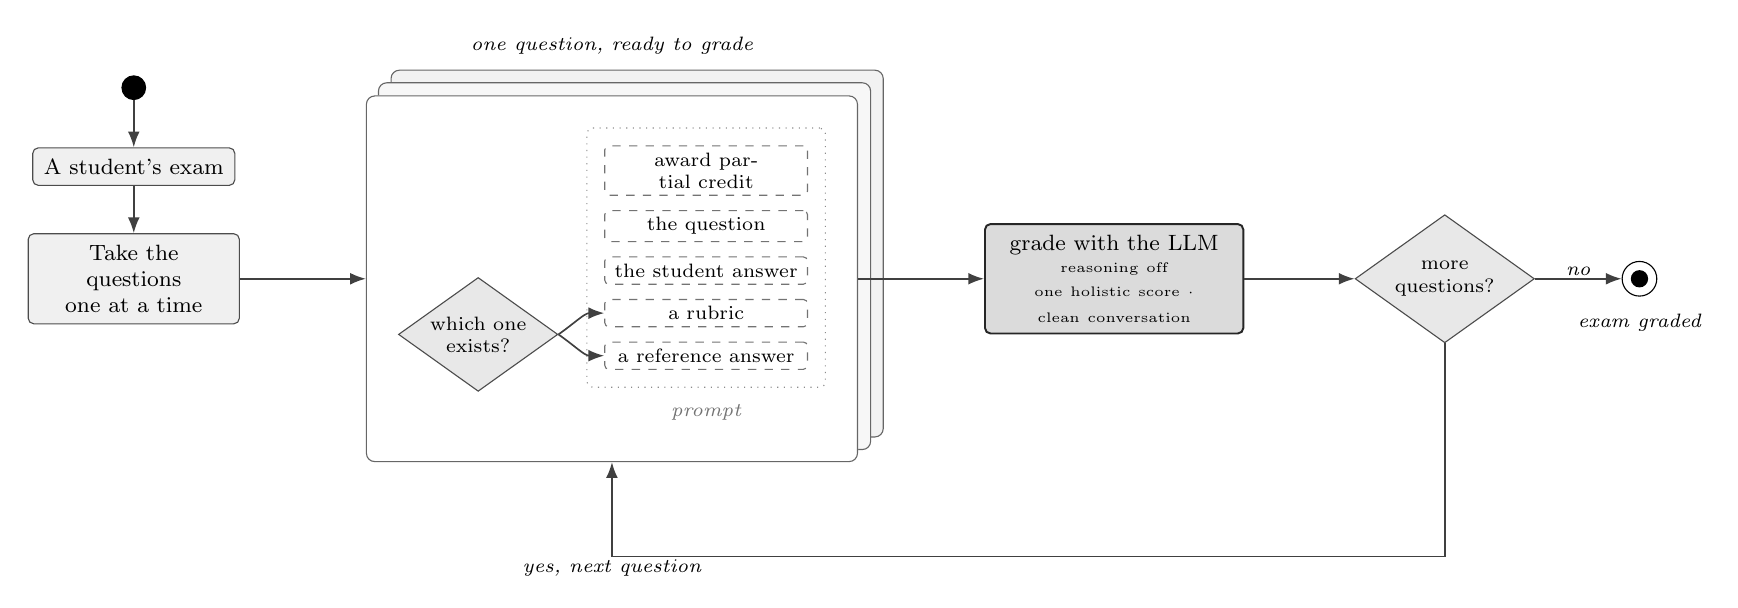
\begin{tikzpicture}[
  font=\footnotesize, >={Latex[length=2mm]},
  proc/.style={rectangle, rounded corners=2pt, draw=black!70, fill=black!6, align=center, inner sep=4pt, font=\footnotesize},
  data/.style={rectangle, rounded corners=1.5pt, draw=black!55, dashed, fill=white, align=center, font=\scriptsize, inner sep=2.5pt},
  dec/.style={diamond, aspect=1.4, draw=black!70, fill=black!9, align=center, inner sep=1pt, font=\scriptsize},
  llm/.style={rectangle, rounded corners=2pt, draw=black!85, line width=0.7pt, fill=black!14, align=center, font=\footnotesize, inner sep=4pt},
  bc/.style={rectangle, rounded corners=3pt, draw=black!60, fill=white, inner sep=4mm},
  start/.style={circle, fill=black, draw=black, minimum size=3mm, inner sep=0pt},
  edgelbl/.style={font=\scriptsize\itshape, fill=white, inner sep=1pt},
  arr/.style={->, draw=black!75, semithick},
]
% --- one block: instruction, question, answer and guidance form the prompt ---
\node[data, text width=24mm] (ins) {award partial credit};
\node[data, text width=24mm, below=1.8mm of ins] (q) {the question};
\node[data, text width=24mm, below=1.8mm of q] (ans) {the student answer};
\node[data, text width=24mm, below=1.8mm of ans] (rub) {a rubric};
\node[data, text width=24mm, below=1.8mm of rub] (ref) {a reference answer};
\coordinate (gmid) at ($(rub.west)!0.5!(ref.west)$);
\node[dec] (cs) at ([xshift=-16mm]gmid) {which one\\exists?};
\draw[arr] (cs.east) to[out=35,in=180] (rub.west);
\draw[arr] (cs.east) to[out=-35,in=180] (ref.west);
\node[draw=black!45, dotted, rounded corners=2pt, inner sep=2.2mm, fit=(ins)(q)(ans)(rub)(ref)] (ctx) {};
\node[font=\scriptsize\itshape, black!55, below=0.9mm of ctx] (ctxlbl) {prompt};
\node[bc, fill=none, fit=(cs)(ctx)(ctxlbl)] (block) {};
\node[font=\scriptsize\itshape, anchor=south] at ([yshift=4mm]block.north) (blocklbl) {one question, ready to grade};
\begin{scope}[on background layer]
  \draw[bc, fill=black!5] ([xshift=3.2mm,yshift=3.2mm]block.south west) rectangle ([xshift=3.2mm,yshift=3.2mm]block.north east);
  \draw[bc, fill=black!3] ([xshift=1.6mm,yshift=1.6mm]block.south west) rectangle ([xshift=1.6mm,yshift=1.6mm]block.north east);
  \fill[white, rounded corners=3pt] (block.south west) rectangle (block.north east);
\end{scope}
% --- start, the exam, and the split ---
\node[proc, left=16mm of block, text width=24mm] (split) {Take the questions one at a time};
\node[proc, above=6mm of split] (exam) {A student's exam};
\node[start, above=6mm of exam] (start) {};
\draw[arr] (start) -- (exam);
\draw[arr] (exam) -- (split);
\draw[arr] (split.east) -- (block.west);
% --- the call: any model, configured by the guide ---
\node[llm, right=16mm of block, text width=30mm] (llm) {grade with the LLM\\[2pt]\tiny reasoning off\\[-1pt]\tiny one holistic score $\cdot$ clean conversation};
\draw[arr] (block.east) -- (llm.west);
% --- loop and the final node ---
\node[dec, right=14mm of llm, text width=15mm] (more) {more questions?};
\node[circle, draw=black, minimum size=4.4mm, inner sep=0pt, right=11mm of more] (end) {};
\fill[black] (end) circle (1.1mm);
\node[font=\scriptsize\itshape, anchor=north] at ([yshift=-1mm]end.south) {exam graded};
\draw[arr] (llm) -- (more);
\draw[arr] (more) -- node[edgelbl,above]{no} (end);
\coordinate (loopbot) at ([yshift=-12mm]block.south);
\draw[arr] (more.south) |- (loopbot) -| node[edgelbl,pos=0.25,below]{yes, next question} (block.south);
\end{tikzpicture}%
}
\caption{The guide at work on one exam. Each question is graded in its own call (the stack stands for the
remaining questions). The prompt, shown dashed, holds the instruction to award partial credit, the question,
the student answer, and the rubric or reference answer that exists for it. The model, with reasoning off,
returns one holistic score in a clean conversation, and the process repeats until every question is graded.}
\label{fig:frameworkdiagram}
\end{figure*}

The guide has six settings (Table~\ref{tab:framework}), and Fig.~\ref{fig:frameworkdiagram} shows it at
work on one exam. Two settings raise agreement: give the model the rubric or the reference answer, and ask
it to award partial credit. The other four keep grading cheap, consistent, and fair: grade with reasoning
off, one question per call, with a single holistic score, in a clean conversation for each answer.
The guide sets how the grader is configured and leaves the choice of model open, so we tested it on all
five models of the study. It returns a score only: feedback for students, and the explanation a grade
needs when it is contested, must come from the rubric or from a separate request.
Fig.~\ref{fig:guideprompt} gives the guide's prompt, in four blocks, with the wording used in the
experiments.

\begin{figure*}[!tb]
\centering
\fbox{\begin{minipage}{0.975\textwidth}\footnotesize\raggedright
\begin{minipage}[t]{0.485\textwidth}\raggedright
\textbf{1. The task} (by domain)\\[2pt]
\emph{Code:} You are an experienced computer-science instructor grading a student's CODE submission for a
programming exam. Assess the LOGICAL correctness of the solution against the problem requirements.
Conceptual understanding and algorithmic correctness take precedence over minor syntax errors. Be
objective and consistent.\\[3pt]
\emph{Short answer:} You are an experienced instructor grading a student's SHORT ANSWER to an exam
question. Assess whether the answer is correct and complete with respect to what the question asks. Be
objective and consistent.
\end{minipage}\hfill
\begin{minipage}[t]{0.485\textwidth}\raggedright
\textbf{2. The guidance and the request for partial credit} (by the guidance available)\\[2pt]
\emph{Rubric:} Use the following question-specific rubric to award marks. Give the marks for every rubric
item the answer satisfies, even when the answer is incomplete or contains errors (for code, even when it
would not compile), and apply any deductions the rubric specifies; do not invent criteria. A partially
correct answer earns partial marks; give 0 only when the answer earns none of the rubric's marks.\\
RUBRIC:\\ $\langle$\emph{the rubric}$\rangle$\\[3pt]
\emph{Reference answer:} Use the following reference answer as the standard of a fully-correct response.
The student answer need not match it word-for-word; judge semantic equivalence. A partially correct
answer earns partial marks; give 0 only when nothing in the answer is correct.\\
REFERENCE ANSWER:\\ $\langle$\emph{the reference answer}$\rangle$
\end{minipage}\\[6pt]
\begin{minipage}[t]{0.485\textwidth}\raggedright
\textbf{3. The question and the answer}\\[2pt]
QUESTION:\\ $\langle$\emph{the question}$\rangle$\\
STUDENT ANSWER:\\ $\langle$\emph{the student answer}$\rangle$
\end{minipage}\hfill
\begin{minipage}[t]{0.485\textwidth}\raggedright
\textbf{4. The output}\\[2pt]
Return ONLY a single JSON object and nothing else (no markdown, no commentary):\\
\{\textquotedbl score\textquotedbl: \textless number between 0 and $\langle$\emph{the maximum
mark}$\rangle$\textgreater\}
\end{minipage}
\end{minipage}}
\caption{The guide's prompt, with the wording used in the experiments. The four blocks are joined in
order into a single message, taking in blocks 1 and 2 the version that fits the task and the guidance
available; the parts in angle brackets are filled in for each answer. Reasoning is switched off through
the model's settings, and the prompt does not mention it.}
\label{fig:guideprompt}
\end{figure*}

\subsection{How the Guide Was Tested}
\label{sec:guidetests}

Two tests compare the guide with every configuration graded in the study, so that it faces every
alternative we ran. Both use the answers the guide was built from.

\emph{Test 1: the guide against the other configurations of the same model.} For each model and
dataset, the guide's configuration is compared with each other configuration of the same model, on the
answers both graded. The alternatives are no guidance, the strict instruction, partial credit with a
justification written first, the whole exam in one call, a score per criterion, one conversation per exam,
and reasoning on. The alternatives other than the instruction ones were graded with the strict
instruction, so they also differ from the guide in that setting. Each comparison uses the same bootstrap
as the results, without correction for multiple comparisons, which makes an advantage of the alternative
easier to detect. Each comparison is then counted as one in which the guide agreed significantly better,
showed no significant difference, or agreed significantly worse.

\emph{Test 2: the guide against the best configuration of any model.} For each dataset, every
configuration graded without reasoning, of any model, is compared on the answers that all of them graded.
The test asks how close the guide comes, with each model, to the best configuration in the study, and
whether any cheaper configuration agrees better. The same comparison on the sampled answers adds the
configurations with reasoning on.

\subsection{Test Results}
\label{sec:guideuse}

%% The figure is defined before the paragraph that first cites it, so that it can take the bottom of that page,
%% or else the top of the next (float rule, CLAUDE.md S9; check_floats.py confirms it follows the reference).
\begin{figure*}[!tb]
\centering
%% Creator: Matplotlib, PGF backend
%%
%% To include the figure in your LaTeX document, write
%%   \input{<filename>.pgf}
%%
%% Make sure the required packages are loaded in your preamble
%%   \usepackage{pgf}
%%
%% Also ensure that all the required font packages are loaded; for instance,
%% the lmodern package is sometimes necessary when using math font.
%%   \usepackage{lmodern}
%%
%% Figures using additional raster images can only be included by \input if
%% they are in the same directory as the main LaTeX file. For loading figures
%% from other directories you can use the `import` package
%%   \usepackage{import}
%%
%% and then include the figures with
%%   \import{<path to file>}{<filename>.pgf}
%%
%% Matplotlib used the following preamble
%%   \def\mathdefault#1{#1}
%%   \everymath=\expandafter{\the\everymath\displaystyle}
%%   \IfFileExists{scrextend.sty}{
%%     \usepackage[fontsize=7.000000pt]{scrextend}
%%   }{
%%     \renewcommand{\normalsize}{\fontsize{7.000000}{8.400000}\selectfont}
%%     \normalsize
%%   }
%%   
%%   \ifdefined\pdftexversion\else  % non-pdftex case.
%%     \usepackage{fontspec}
%%     \setmainfont{DejaVuSerif.ttf}[Path=\detokenize{/Users/pedroromano/Projetos/PhD/phd-paper2-configuration-framework-for-llm-based-grading/.venv/lib/python3.13/site-packages/matplotlib/mpl-data/fonts/ttf/}]
%%     \setsansfont{DejaVuSans.ttf}[Path=\detokenize{/Users/pedroromano/Projetos/PhD/phd-paper2-configuration-framework-for-llm-based-grading/.venv/lib/python3.13/site-packages/matplotlib/mpl-data/fonts/ttf/}]
%%     \setmonofont{DejaVuSansMono.ttf}[Path=\detokenize{/Users/pedroromano/Projetos/PhD/phd-paper2-configuration-framework-for-llm-based-grading/.venv/lib/python3.13/site-packages/matplotlib/mpl-data/fonts/ttf/}]
%%   \fi
%%   \makeatletter\@ifpackageloaded{underscore}{}{\usepackage[strings]{underscore}}\makeatother
%%
\begingroup%
\makeatletter%
\begin{pgfpicture}%
\pgfpathrectangle{\pgfpointorigin}{\pgfqpoint{6.847850in}{3.565173in}}%
\pgfusepath{use as bounding box, clip}%
\begin{pgfscope}%
\pgfsetbuttcap%
\pgfsetmiterjoin%
\definecolor{currentfill}{rgb}{1.000000,1.000000,1.000000}%
\pgfsetfillcolor{currentfill}%
\pgfsetlinewidth{0.000000pt}%
\definecolor{currentstroke}{rgb}{1.000000,1.000000,1.000000}%
\pgfsetstrokecolor{currentstroke}%
\pgfsetdash{}{0pt}%
\pgfpathmoveto{\pgfqpoint{0.000000in}{-0.000000in}}%
\pgfpathlineto{\pgfqpoint{6.847850in}{-0.000000in}}%
\pgfpathlineto{\pgfqpoint{6.847850in}{3.565173in}}%
\pgfpathlineto{\pgfqpoint{0.000000in}{3.565173in}}%
\pgfpathlineto{\pgfqpoint{0.000000in}{-0.000000in}}%
\pgfpathclose%
\pgfusepath{fill}%
\end{pgfscope}%
\begin{pgfscope}%
\pgfsetbuttcap%
\pgfsetmiterjoin%
\definecolor{currentfill}{rgb}{1.000000,1.000000,1.000000}%
\pgfsetfillcolor{currentfill}%
\pgfsetlinewidth{0.000000pt}%
\definecolor{currentstroke}{rgb}{0.000000,0.000000,0.000000}%
\pgfsetstrokecolor{currentstroke}%
\pgfsetstrokeopacity{0.000000}%
\pgfsetdash{}{0pt}%
\pgfpathmoveto{\pgfqpoint{1.274781in}{0.993424in}}%
\pgfpathlineto{\pgfqpoint{3.407261in}{0.993424in}}%
\pgfpathlineto{\pgfqpoint{3.407261in}{3.203599in}}%
\pgfpathlineto{\pgfqpoint{1.274781in}{3.203599in}}%
\pgfpathlineto{\pgfqpoint{1.274781in}{0.993424in}}%
\pgfpathclose%
\pgfusepath{fill}%
\end{pgfscope}%
\begin{pgfscope}%
\pgfpathrectangle{\pgfqpoint{1.274781in}{0.993424in}}{\pgfqpoint{2.132480in}{2.210175in}}%
\pgfusepath{clip}%
\pgfsetbuttcap%
\pgfsetmiterjoin%
\definecolor{currentfill}{rgb}{0.239216,0.239216,0.239216}%
\pgfsetfillcolor{currentfill}%
\pgfsetlinewidth{0.602250pt}%
\definecolor{currentstroke}{rgb}{1.000000,1.000000,1.000000}%
\pgfsetstrokecolor{currentstroke}%
\pgfsetdash{}{0pt}%
\pgfpathmoveto{\pgfqpoint{1.274781in}{2.937207in}}%
\pgfpathlineto{\pgfqpoint{2.980765in}{2.937207in}}%
\pgfpathlineto{\pgfqpoint{2.980765in}{3.118705in}}%
\pgfpathlineto{\pgfqpoint{1.274781in}{3.118705in}}%
\pgfpathlineto{\pgfqpoint{1.274781in}{2.937207in}}%
\pgfpathclose%
\pgfusepath{stroke,fill}%
\end{pgfscope}%
\begin{pgfscope}%
\pgfpathrectangle{\pgfqpoint{1.274781in}{0.993424in}}{\pgfqpoint{2.132480in}{2.210175in}}%
\pgfusepath{clip}%
\pgfsetbuttcap%
\pgfsetmiterjoin%
\definecolor{currentfill}{rgb}{0.800000,0.800000,0.800000}%
\pgfsetfillcolor{currentfill}%
\pgfsetlinewidth{0.602250pt}%
\definecolor{currentstroke}{rgb}{1.000000,1.000000,1.000000}%
\pgfsetstrokecolor{currentstroke}%
\pgfsetdash{}{0pt}%
\pgfpathmoveto{\pgfqpoint{2.980765in}{2.937207in}}%
\pgfpathlineto{\pgfqpoint{3.407261in}{2.937207in}}%
\pgfpathlineto{\pgfqpoint{3.407261in}{3.118705in}}%
\pgfpathlineto{\pgfqpoint{2.980765in}{3.118705in}}%
\pgfpathlineto{\pgfqpoint{2.980765in}{2.937207in}}%
\pgfpathclose%
\pgfusepath{stroke,fill}%
\end{pgfscope}%
\begin{pgfscope}%
\pgfpathrectangle{\pgfqpoint{1.274781in}{0.993424in}}{\pgfqpoint{2.132480in}{2.210175in}}%
\pgfusepath{clip}%
\pgfsetbuttcap%
\pgfsetmiterjoin%
\definecolor{currentfill}{rgb}{0.239216,0.239216,0.239216}%
\pgfsetfillcolor{currentfill}%
\pgfsetlinewidth{0.602250pt}%
\definecolor{currentstroke}{rgb}{1.000000,1.000000,1.000000}%
\pgfsetstrokecolor{currentstroke}%
\pgfsetdash{}{0pt}%
\pgfpathmoveto{\pgfqpoint{1.274781in}{2.644469in}}%
\pgfpathlineto{\pgfqpoint{2.147159in}{2.644469in}}%
\pgfpathlineto{\pgfqpoint{2.147159in}{2.825967in}}%
\pgfpathlineto{\pgfqpoint{1.274781in}{2.825967in}}%
\pgfpathlineto{\pgfqpoint{1.274781in}{2.644469in}}%
\pgfpathclose%
\pgfusepath{stroke,fill}%
\end{pgfscope}%
\begin{pgfscope}%
\pgfpathrectangle{\pgfqpoint{1.274781in}{0.993424in}}{\pgfqpoint{2.132480in}{2.210175in}}%
\pgfusepath{clip}%
\pgfsetbuttcap%
\pgfsetmiterjoin%
\definecolor{currentfill}{rgb}{0.800000,0.800000,0.800000}%
\pgfsetfillcolor{currentfill}%
\pgfsetlinewidth{0.602250pt}%
\definecolor{currentstroke}{rgb}{1.000000,1.000000,1.000000}%
\pgfsetstrokecolor{currentstroke}%
\pgfsetdash{}{0pt}%
\pgfpathmoveto{\pgfqpoint{2.147159in}{2.644469in}}%
\pgfpathlineto{\pgfqpoint{3.310331in}{2.644469in}}%
\pgfpathlineto{\pgfqpoint{3.310331in}{2.825967in}}%
\pgfpathlineto{\pgfqpoint{2.147159in}{2.825967in}}%
\pgfpathlineto{\pgfqpoint{2.147159in}{2.644469in}}%
\pgfpathclose%
\pgfusepath{stroke,fill}%
\end{pgfscope}%
\begin{pgfscope}%
\pgfpathrectangle{\pgfqpoint{1.274781in}{0.993424in}}{\pgfqpoint{2.132480in}{2.210175in}}%
\pgfusepath{clip}%
\pgfsetbuttcap%
\pgfsetmiterjoin%
\definecolor{currentfill}{rgb}{0.941176,0.894118,0.258824}%
\pgfsetfillcolor{currentfill}%
\pgfsetlinewidth{0.602250pt}%
\definecolor{currentstroke}{rgb}{1.000000,1.000000,1.000000}%
\pgfsetstrokecolor{currentstroke}%
\pgfsetdash{}{0pt}%
\pgfpathmoveto{\pgfqpoint{3.310331in}{2.644469in}}%
\pgfpathlineto{\pgfqpoint{3.407261in}{2.644469in}}%
\pgfpathlineto{\pgfqpoint{3.407261in}{2.825967in}}%
\pgfpathlineto{\pgfqpoint{3.310331in}{2.825967in}}%
\pgfpathlineto{\pgfqpoint{3.310331in}{2.644469in}}%
\pgfpathclose%
\pgfusepath{stroke,fill}%
\end{pgfscope}%
\begin{pgfscope}%
\pgfpathrectangle{\pgfqpoint{1.274781in}{0.993424in}}{\pgfqpoint{2.132480in}{2.210175in}}%
\pgfusepath{clip}%
\pgfsetbuttcap%
\pgfsetmiterjoin%
\definecolor{currentfill}{rgb}{0.239216,0.239216,0.239216}%
\pgfsetfillcolor{currentfill}%
\pgfsetlinewidth{0.602250pt}%
\definecolor{currentstroke}{rgb}{1.000000,1.000000,1.000000}%
\pgfsetstrokecolor{currentstroke}%
\pgfsetdash{}{0pt}%
\pgfpathmoveto{\pgfqpoint{1.274781in}{2.351731in}}%
\pgfpathlineto{\pgfqpoint{1.807901in}{2.351731in}}%
\pgfpathlineto{\pgfqpoint{1.807901in}{2.533228in}}%
\pgfpathlineto{\pgfqpoint{1.274781in}{2.533228in}}%
\pgfpathlineto{\pgfqpoint{1.274781in}{2.351731in}}%
\pgfpathclose%
\pgfusepath{stroke,fill}%
\end{pgfscope}%
\begin{pgfscope}%
\pgfpathrectangle{\pgfqpoint{1.274781in}{0.993424in}}{\pgfqpoint{2.132480in}{2.210175in}}%
\pgfusepath{clip}%
\pgfsetbuttcap%
\pgfsetmiterjoin%
\definecolor{currentfill}{rgb}{0.800000,0.800000,0.800000}%
\pgfsetfillcolor{currentfill}%
\pgfsetlinewidth{0.602250pt}%
\definecolor{currentstroke}{rgb}{1.000000,1.000000,1.000000}%
\pgfsetstrokecolor{currentstroke}%
\pgfsetdash{}{0pt}%
\pgfpathmoveto{\pgfqpoint{1.807901in}{2.351731in}}%
\pgfpathlineto{\pgfqpoint{3.407261in}{2.351731in}}%
\pgfpathlineto{\pgfqpoint{3.407261in}{2.533228in}}%
\pgfpathlineto{\pgfqpoint{1.807901in}{2.533228in}}%
\pgfpathlineto{\pgfqpoint{1.807901in}{2.351731in}}%
\pgfpathclose%
\pgfusepath{stroke,fill}%
\end{pgfscope}%
\begin{pgfscope}%
\pgfpathrectangle{\pgfqpoint{1.274781in}{0.993424in}}{\pgfqpoint{2.132480in}{2.210175in}}%
\pgfusepath{clip}%
\pgfsetbuttcap%
\pgfsetmiterjoin%
\definecolor{currentfill}{rgb}{0.239216,0.239216,0.239216}%
\pgfsetfillcolor{currentfill}%
\pgfsetlinewidth{0.602250pt}%
\definecolor{currentstroke}{rgb}{1.000000,1.000000,1.000000}%
\pgfsetstrokecolor{currentstroke}%
\pgfsetdash{}{0pt}%
\pgfpathmoveto{\pgfqpoint{1.274781in}{2.058992in}}%
\pgfpathlineto{\pgfqpoint{3.407261in}{2.058992in}}%
\pgfpathlineto{\pgfqpoint{3.407261in}{2.240490in}}%
\pgfpathlineto{\pgfqpoint{1.274781in}{2.240490in}}%
\pgfpathlineto{\pgfqpoint{1.274781in}{2.058992in}}%
\pgfpathclose%
\pgfusepath{stroke,fill}%
\end{pgfscope}%
\begin{pgfscope}%
\pgfpathrectangle{\pgfqpoint{1.274781in}{0.993424in}}{\pgfqpoint{2.132480in}{2.210175in}}%
\pgfusepath{clip}%
\pgfsetbuttcap%
\pgfsetmiterjoin%
\definecolor{currentfill}{rgb}{0.239216,0.239216,0.239216}%
\pgfsetfillcolor{currentfill}%
\pgfsetlinewidth{0.602250pt}%
\definecolor{currentstroke}{rgb}{1.000000,1.000000,1.000000}%
\pgfsetstrokecolor{currentstroke}%
\pgfsetdash{}{0pt}%
\pgfpathmoveto{\pgfqpoint{1.274781in}{1.766254in}}%
\pgfpathlineto{\pgfqpoint{2.696435in}{1.766254in}}%
\pgfpathlineto{\pgfqpoint{2.696435in}{1.947752in}}%
\pgfpathlineto{\pgfqpoint{1.274781in}{1.947752in}}%
\pgfpathlineto{\pgfqpoint{1.274781in}{1.766254in}}%
\pgfpathclose%
\pgfusepath{stroke,fill}%
\end{pgfscope}%
\begin{pgfscope}%
\pgfpathrectangle{\pgfqpoint{1.274781in}{0.993424in}}{\pgfqpoint{2.132480in}{2.210175in}}%
\pgfusepath{clip}%
\pgfsetbuttcap%
\pgfsetmiterjoin%
\definecolor{currentfill}{rgb}{0.800000,0.800000,0.800000}%
\pgfsetfillcolor{currentfill}%
\pgfsetlinewidth{0.602250pt}%
\definecolor{currentstroke}{rgb}{1.000000,1.000000,1.000000}%
\pgfsetstrokecolor{currentstroke}%
\pgfsetdash{}{0pt}%
\pgfpathmoveto{\pgfqpoint{2.696435in}{1.766254in}}%
\pgfpathlineto{\pgfqpoint{3.407261in}{1.766254in}}%
\pgfpathlineto{\pgfqpoint{3.407261in}{1.947752in}}%
\pgfpathlineto{\pgfqpoint{2.696435in}{1.947752in}}%
\pgfpathlineto{\pgfqpoint{2.696435in}{1.766254in}}%
\pgfpathclose%
\pgfusepath{stroke,fill}%
\end{pgfscope}%
\begin{pgfscope}%
\pgfpathrectangle{\pgfqpoint{1.274781in}{0.993424in}}{\pgfqpoint{2.132480in}{2.210175in}}%
\pgfusepath{clip}%
\pgfsetbuttcap%
\pgfsetmiterjoin%
\definecolor{currentfill}{rgb}{0.239216,0.239216,0.239216}%
\pgfsetfillcolor{currentfill}%
\pgfsetlinewidth{0.602250pt}%
\definecolor{currentstroke}{rgb}{1.000000,1.000000,1.000000}%
\pgfsetstrokecolor{currentstroke}%
\pgfsetdash{}{0pt}%
\pgfpathmoveto{\pgfqpoint{1.274781in}{1.473515in}}%
\pgfpathlineto{\pgfqpoint{2.341021in}{1.473515in}}%
\pgfpathlineto{\pgfqpoint{2.341021in}{1.655013in}}%
\pgfpathlineto{\pgfqpoint{1.274781in}{1.655013in}}%
\pgfpathlineto{\pgfqpoint{1.274781in}{1.473515in}}%
\pgfpathclose%
\pgfusepath{stroke,fill}%
\end{pgfscope}%
\begin{pgfscope}%
\pgfpathrectangle{\pgfqpoint{1.274781in}{0.993424in}}{\pgfqpoint{2.132480in}{2.210175in}}%
\pgfusepath{clip}%
\pgfsetbuttcap%
\pgfsetmiterjoin%
\definecolor{currentfill}{rgb}{0.800000,0.800000,0.800000}%
\pgfsetfillcolor{currentfill}%
\pgfsetlinewidth{0.602250pt}%
\definecolor{currentstroke}{rgb}{1.000000,1.000000,1.000000}%
\pgfsetstrokecolor{currentstroke}%
\pgfsetdash{}{0pt}%
\pgfpathmoveto{\pgfqpoint{2.341021in}{1.473515in}}%
\pgfpathlineto{\pgfqpoint{3.407261in}{1.473515in}}%
\pgfpathlineto{\pgfqpoint{3.407261in}{1.655013in}}%
\pgfpathlineto{\pgfqpoint{2.341021in}{1.655013in}}%
\pgfpathlineto{\pgfqpoint{2.341021in}{1.473515in}}%
\pgfpathclose%
\pgfusepath{stroke,fill}%
\end{pgfscope}%
\begin{pgfscope}%
\pgfpathrectangle{\pgfqpoint{1.274781in}{0.993424in}}{\pgfqpoint{2.132480in}{2.210175in}}%
\pgfusepath{clip}%
\pgfsetbuttcap%
\pgfsetmiterjoin%
\definecolor{currentfill}{rgb}{0.800000,0.800000,0.800000}%
\pgfsetfillcolor{currentfill}%
\pgfsetlinewidth{0.602250pt}%
\definecolor{currentstroke}{rgb}{1.000000,1.000000,1.000000}%
\pgfsetstrokecolor{currentstroke}%
\pgfsetdash{}{0pt}%
\pgfpathmoveto{\pgfqpoint{1.274781in}{1.078319in}}%
\pgfpathlineto{\pgfqpoint{2.529181in}{1.078319in}}%
\pgfpathlineto{\pgfqpoint{2.529181in}{1.259816in}}%
\pgfpathlineto{\pgfqpoint{1.274781in}{1.259816in}}%
\pgfpathlineto{\pgfqpoint{1.274781in}{1.078319in}}%
\pgfpathclose%
\pgfusepath{stroke,fill}%
\end{pgfscope}%
\begin{pgfscope}%
\pgfpathrectangle{\pgfqpoint{1.274781in}{0.993424in}}{\pgfqpoint{2.132480in}{2.210175in}}%
\pgfusepath{clip}%
\pgfsetbuttcap%
\pgfsetmiterjoin%
\definecolor{currentfill}{rgb}{0.941176,0.894118,0.258824}%
\pgfsetfillcolor{currentfill}%
\pgfsetlinewidth{0.602250pt}%
\definecolor{currentstroke}{rgb}{1.000000,1.000000,1.000000}%
\pgfsetstrokecolor{currentstroke}%
\pgfsetdash{}{0pt}%
\pgfpathmoveto{\pgfqpoint{2.529181in}{1.078319in}}%
\pgfpathlineto{\pgfqpoint{3.407261in}{1.078319in}}%
\pgfpathlineto{\pgfqpoint{3.407261in}{1.259816in}}%
\pgfpathlineto{\pgfqpoint{2.529181in}{1.259816in}}%
\pgfpathlineto{\pgfqpoint{2.529181in}{1.078319in}}%
\pgfpathclose%
\pgfusepath{stroke,fill}%
\end{pgfscope}%
\begin{pgfscope}%
\pgfpathrectangle{\pgfqpoint{1.274781in}{0.993424in}}{\pgfqpoint{2.132480in}{2.210175in}}%
\pgfusepath{clip}%
\pgfsetrectcap%
\pgfsetroundjoin%
\pgfsetlinewidth{0.803000pt}%
\definecolor{currentstroke}{rgb}{0.690196,0.690196,0.690196}%
\pgfsetstrokecolor{currentstroke}%
\pgfsetstrokeopacity{0.250000}%
\pgfsetdash{}{0pt}%
\pgfpathmoveto{\pgfqpoint{1.274781in}{0.993424in}}%
\pgfpathlineto{\pgfqpoint{1.274781in}{3.203599in}}%
\pgfusepath{stroke}%
\end{pgfscope}%
\begin{pgfscope}%
\pgfsetbuttcap%
\pgfsetroundjoin%
\definecolor{currentfill}{rgb}{0.000000,0.000000,0.000000}%
\pgfsetfillcolor{currentfill}%
\pgfsetlinewidth{0.803000pt}%
\definecolor{currentstroke}{rgb}{0.000000,0.000000,0.000000}%
\pgfsetstrokecolor{currentstroke}%
\pgfsetdash{}{0pt}%
\pgfsys@defobject{currentmarker}{\pgfqpoint{0.000000in}{-0.048611in}}{\pgfqpoint{0.000000in}{0.000000in}}{%
\pgfpathmoveto{\pgfqpoint{0.000000in}{0.000000in}}%
\pgfpathlineto{\pgfqpoint{0.000000in}{-0.048611in}}%
\pgfusepath{stroke,fill}%
}%
\begin{pgfscope}%
\pgfsys@transformshift{1.274781in}{0.993424in}%
\pgfsys@useobject{currentmarker}{}%
\end{pgfscope}%
\end{pgfscope}%
\begin{pgfscope}%
\definecolor{textcolor}{rgb}{0.000000,0.000000,0.000000}%
\pgfsetstrokecolor{textcolor}%
\pgfsetfillcolor{textcolor}%
\pgftext[x=1.274781in,y=0.896202in,,top]{\color{textcolor}{\sffamily\fontsize{6.500000}{7.800000}\selectfont\catcode`\^=\active\def^{\ifmmode\sp\else\^{}\fi}\catcode`\%=\active\def%{\%}0\%}}%
\end{pgfscope}%
\begin{pgfscope}%
\pgfpathrectangle{\pgfqpoint{1.274781in}{0.993424in}}{\pgfqpoint{2.132480in}{2.210175in}}%
\pgfusepath{clip}%
\pgfsetrectcap%
\pgfsetroundjoin%
\pgfsetlinewidth{0.803000pt}%
\definecolor{currentstroke}{rgb}{0.690196,0.690196,0.690196}%
\pgfsetstrokecolor{currentstroke}%
\pgfsetstrokeopacity{0.250000}%
\pgfsetdash{}{0pt}%
\pgfpathmoveto{\pgfqpoint{1.807901in}{0.993424in}}%
\pgfpathlineto{\pgfqpoint{1.807901in}{3.203599in}}%
\pgfusepath{stroke}%
\end{pgfscope}%
\begin{pgfscope}%
\pgfsetbuttcap%
\pgfsetroundjoin%
\definecolor{currentfill}{rgb}{0.000000,0.000000,0.000000}%
\pgfsetfillcolor{currentfill}%
\pgfsetlinewidth{0.803000pt}%
\definecolor{currentstroke}{rgb}{0.000000,0.000000,0.000000}%
\pgfsetstrokecolor{currentstroke}%
\pgfsetdash{}{0pt}%
\pgfsys@defobject{currentmarker}{\pgfqpoint{0.000000in}{-0.048611in}}{\pgfqpoint{0.000000in}{0.000000in}}{%
\pgfpathmoveto{\pgfqpoint{0.000000in}{0.000000in}}%
\pgfpathlineto{\pgfqpoint{0.000000in}{-0.048611in}}%
\pgfusepath{stroke,fill}%
}%
\begin{pgfscope}%
\pgfsys@transformshift{1.807901in}{0.993424in}%
\pgfsys@useobject{currentmarker}{}%
\end{pgfscope}%
\end{pgfscope}%
\begin{pgfscope}%
\definecolor{textcolor}{rgb}{0.000000,0.000000,0.000000}%
\pgfsetstrokecolor{textcolor}%
\pgfsetfillcolor{textcolor}%
\pgftext[x=1.807901in,y=0.896202in,,top]{\color{textcolor}{\sffamily\fontsize{6.500000}{7.800000}\selectfont\catcode`\^=\active\def^{\ifmmode\sp\else\^{}\fi}\catcode`\%=\active\def%{\%}25\%}}%
\end{pgfscope}%
\begin{pgfscope}%
\pgfpathrectangle{\pgfqpoint{1.274781in}{0.993424in}}{\pgfqpoint{2.132480in}{2.210175in}}%
\pgfusepath{clip}%
\pgfsetrectcap%
\pgfsetroundjoin%
\pgfsetlinewidth{0.803000pt}%
\definecolor{currentstroke}{rgb}{0.690196,0.690196,0.690196}%
\pgfsetstrokecolor{currentstroke}%
\pgfsetstrokeopacity{0.250000}%
\pgfsetdash{}{0pt}%
\pgfpathmoveto{\pgfqpoint{2.341021in}{0.993424in}}%
\pgfpathlineto{\pgfqpoint{2.341021in}{3.203599in}}%
\pgfusepath{stroke}%
\end{pgfscope}%
\begin{pgfscope}%
\pgfsetbuttcap%
\pgfsetroundjoin%
\definecolor{currentfill}{rgb}{0.000000,0.000000,0.000000}%
\pgfsetfillcolor{currentfill}%
\pgfsetlinewidth{0.803000pt}%
\definecolor{currentstroke}{rgb}{0.000000,0.000000,0.000000}%
\pgfsetstrokecolor{currentstroke}%
\pgfsetdash{}{0pt}%
\pgfsys@defobject{currentmarker}{\pgfqpoint{0.000000in}{-0.048611in}}{\pgfqpoint{0.000000in}{0.000000in}}{%
\pgfpathmoveto{\pgfqpoint{0.000000in}{0.000000in}}%
\pgfpathlineto{\pgfqpoint{0.000000in}{-0.048611in}}%
\pgfusepath{stroke,fill}%
}%
\begin{pgfscope}%
\pgfsys@transformshift{2.341021in}{0.993424in}%
\pgfsys@useobject{currentmarker}{}%
\end{pgfscope}%
\end{pgfscope}%
\begin{pgfscope}%
\definecolor{textcolor}{rgb}{0.000000,0.000000,0.000000}%
\pgfsetstrokecolor{textcolor}%
\pgfsetfillcolor{textcolor}%
\pgftext[x=2.341021in,y=0.896202in,,top]{\color{textcolor}{\sffamily\fontsize{6.500000}{7.800000}\selectfont\catcode`\^=\active\def^{\ifmmode\sp\else\^{}\fi}\catcode`\%=\active\def%{\%}50\%}}%
\end{pgfscope}%
\begin{pgfscope}%
\pgfpathrectangle{\pgfqpoint{1.274781in}{0.993424in}}{\pgfqpoint{2.132480in}{2.210175in}}%
\pgfusepath{clip}%
\pgfsetrectcap%
\pgfsetroundjoin%
\pgfsetlinewidth{0.803000pt}%
\definecolor{currentstroke}{rgb}{0.690196,0.690196,0.690196}%
\pgfsetstrokecolor{currentstroke}%
\pgfsetstrokeopacity{0.250000}%
\pgfsetdash{}{0pt}%
\pgfpathmoveto{\pgfqpoint{2.874141in}{0.993424in}}%
\pgfpathlineto{\pgfqpoint{2.874141in}{3.203599in}}%
\pgfusepath{stroke}%
\end{pgfscope}%
\begin{pgfscope}%
\pgfsetbuttcap%
\pgfsetroundjoin%
\definecolor{currentfill}{rgb}{0.000000,0.000000,0.000000}%
\pgfsetfillcolor{currentfill}%
\pgfsetlinewidth{0.803000pt}%
\definecolor{currentstroke}{rgb}{0.000000,0.000000,0.000000}%
\pgfsetstrokecolor{currentstroke}%
\pgfsetdash{}{0pt}%
\pgfsys@defobject{currentmarker}{\pgfqpoint{0.000000in}{-0.048611in}}{\pgfqpoint{0.000000in}{0.000000in}}{%
\pgfpathmoveto{\pgfqpoint{0.000000in}{0.000000in}}%
\pgfpathlineto{\pgfqpoint{0.000000in}{-0.048611in}}%
\pgfusepath{stroke,fill}%
}%
\begin{pgfscope}%
\pgfsys@transformshift{2.874141in}{0.993424in}%
\pgfsys@useobject{currentmarker}{}%
\end{pgfscope}%
\end{pgfscope}%
\begin{pgfscope}%
\definecolor{textcolor}{rgb}{0.000000,0.000000,0.000000}%
\pgfsetstrokecolor{textcolor}%
\pgfsetfillcolor{textcolor}%
\pgftext[x=2.874141in,y=0.896202in,,top]{\color{textcolor}{\sffamily\fontsize{6.500000}{7.800000}\selectfont\catcode`\^=\active\def^{\ifmmode\sp\else\^{}\fi}\catcode`\%=\active\def%{\%}75\%}}%
\end{pgfscope}%
\begin{pgfscope}%
\pgfpathrectangle{\pgfqpoint{1.274781in}{0.993424in}}{\pgfqpoint{2.132480in}{2.210175in}}%
\pgfusepath{clip}%
\pgfsetrectcap%
\pgfsetroundjoin%
\pgfsetlinewidth{0.803000pt}%
\definecolor{currentstroke}{rgb}{0.690196,0.690196,0.690196}%
\pgfsetstrokecolor{currentstroke}%
\pgfsetstrokeopacity{0.250000}%
\pgfsetdash{}{0pt}%
\pgfpathmoveto{\pgfqpoint{3.407261in}{0.993424in}}%
\pgfpathlineto{\pgfqpoint{3.407261in}{3.203599in}}%
\pgfusepath{stroke}%
\end{pgfscope}%
\begin{pgfscope}%
\pgfsetbuttcap%
\pgfsetroundjoin%
\definecolor{currentfill}{rgb}{0.000000,0.000000,0.000000}%
\pgfsetfillcolor{currentfill}%
\pgfsetlinewidth{0.803000pt}%
\definecolor{currentstroke}{rgb}{0.000000,0.000000,0.000000}%
\pgfsetstrokecolor{currentstroke}%
\pgfsetdash{}{0pt}%
\pgfsys@defobject{currentmarker}{\pgfqpoint{0.000000in}{-0.048611in}}{\pgfqpoint{0.000000in}{0.000000in}}{%
\pgfpathmoveto{\pgfqpoint{0.000000in}{0.000000in}}%
\pgfpathlineto{\pgfqpoint{0.000000in}{-0.048611in}}%
\pgfusepath{stroke,fill}%
}%
\begin{pgfscope}%
\pgfsys@transformshift{3.407261in}{0.993424in}%
\pgfsys@useobject{currentmarker}{}%
\end{pgfscope}%
\end{pgfscope}%
\begin{pgfscope}%
\definecolor{textcolor}{rgb}{0.000000,0.000000,0.000000}%
\pgfsetstrokecolor{textcolor}%
\pgfsetfillcolor{textcolor}%
\pgftext[x=3.407261in,y=0.896202in,,top]{\color{textcolor}{\sffamily\fontsize{6.500000}{7.800000}\selectfont\catcode`\^=\active\def^{\ifmmode\sp\else\^{}\fi}\catcode`\%=\active\def%{\%}100\%}}%
\end{pgfscope}%
\begin{pgfscope}%
\definecolor{textcolor}{rgb}{0.000000,0.000000,0.000000}%
\pgfsetstrokecolor{textcolor}%
\pgfsetfillcolor{textcolor}%
\pgftext[x=2.341021in,y=0.766573in,,top]{\color{textcolor}{\sffamily\fontsize{7.500000}{9.000000}\selectfont\catcode`\^=\active\def^{\ifmmode\sp\else\^{}\fi}\catcode`\%=\active\def%{\%}share of the comparisons (model $\times$ dataset)}}%
\end{pgfscope}%
\begin{pgfscope}%
\definecolor{textcolor}{rgb}{0.000000,0.000000,0.000000}%
\pgfsetstrokecolor{textcolor}%
\pgfsetfillcolor{textcolor}%
\pgftext[x=0.461116in, y=2.996706in, left, base]{\color{textcolor}{\sffamily\fontsize{6.500000}{7.800000}\selectfont\catcode`\^=\active\def^{\ifmmode\sp\else\^{}\fi}\catcode`\%=\active\def%{\%}No guidance (15)}}%
\end{pgfscope}%
\begin{pgfscope}%
\definecolor{textcolor}{rgb}{0.000000,0.000000,0.000000}%
\pgfsetstrokecolor{textcolor}%
\pgfsetfillcolor{textcolor}%
\pgftext[x=0.296675in, y=2.703968in, left, base]{\color{textcolor}{\sffamily\fontsize{6.500000}{7.800000}\selectfont\catcode`\^=\active\def^{\ifmmode\sp\else\^{}\fi}\catcode`\%=\active\def%{\%}Strict instruction (22)}}%
\end{pgfscope}%
\begin{pgfscope}%
\definecolor{textcolor}{rgb}{0.000000,0.000000,0.000000}%
\pgfsetstrokecolor{textcolor}%
\pgfsetfillcolor{textcolor}%
\pgftext[x=0.252693in, y=2.411230in, left, base]{\color{textcolor}{\sffamily\fontsize{6.500000}{7.800000}\selectfont\catcode`\^=\active\def^{\ifmmode\sp\else\^{}\fi}\catcode`\%=\active\def%{\%}With a justification (4)}}%
\end{pgfscope}%
\begin{pgfscope}%
\definecolor{textcolor}{rgb}{0.000000,0.000000,0.000000}%
\pgfsetstrokecolor{textcolor}%
\pgfsetfillcolor{textcolor}%
\pgftext[x=0.100000in, y=2.118491in, left, base]{\color{textcolor}{\sffamily\fontsize{6.500000}{7.800000}\selectfont\catcode`\^=\active\def^{\ifmmode\sp\else\^{}\fi}\catcode`\%=\active\def%{\%}Whole exam in one call (3)}}%
\end{pgfscope}%
\begin{pgfscope}%
\definecolor{textcolor}{rgb}{0.000000,0.000000,0.000000}%
\pgfsetstrokecolor{textcolor}%
\pgfsetfillcolor{textcolor}%
\pgftext[x=0.285332in, y=1.825753in, left, base]{\color{textcolor}{\sffamily\fontsize{6.500000}{7.800000}\selectfont\catcode`\^=\active\def^{\ifmmode\sp\else\^{}\fi}\catcode`\%=\active\def%{\%}Score per criterion (6)}}%
\end{pgfscope}%
\begin{pgfscope}%
\definecolor{textcolor}{rgb}{0.000000,0.000000,0.000000}%
\pgfsetstrokecolor{textcolor}%
\pgfsetfillcolor{textcolor}%
\pgftext[x=0.226362in, y=1.533014in, left, base]{\color{textcolor}{\sffamily\fontsize{6.500000}{7.800000}\selectfont\catcode`\^=\active\def^{\ifmmode\sp\else\^{}\fi}\catcode`\%=\active\def%{\%}Shared conversation (6)}}%
\end{pgfscope}%
\begin{pgfscope}%
\definecolor{textcolor}{rgb}{0.000000,0.000000,0.000000}%
\pgfsetstrokecolor{textcolor}%
\pgfsetfillcolor{textcolor}%
\pgftext[x=0.427463in, y=1.137817in, left, base]{\color{textcolor}{\sffamily\fontsize{6.500000}{7.800000}\selectfont\catcode`\^=\active\def^{\ifmmode\sp\else\^{}\fi}\catcode`\%=\active\def%{\%}Reasoning on (17)}}%
\end{pgfscope}%
\begin{pgfscope}%
\pgfpathrectangle{\pgfqpoint{1.274781in}{0.993424in}}{\pgfqpoint{2.132480in}{2.210175in}}%
\pgfusepath{clip}%
\pgfsetbuttcap%
\pgfsetroundjoin%
\pgfsetlinewidth{0.501875pt}%
\definecolor{currentstroke}{rgb}{0.600000,0.600000,0.600000}%
\pgfsetstrokecolor{currentstroke}%
\pgfsetdash{{0.500000pt}{0.825000pt}}{0.000000pt}%
\pgfpathmoveto{\pgfqpoint{1.274781in}{1.366666in}}%
\pgfpathlineto{\pgfqpoint{3.407261in}{1.366666in}}%
\pgfusepath{stroke}%
\end{pgfscope}%
\begin{pgfscope}%
\pgfsetrectcap%
\pgfsetmiterjoin%
\pgfsetlinewidth{0.803000pt}%
\definecolor{currentstroke}{rgb}{0.000000,0.000000,0.000000}%
\pgfsetstrokecolor{currentstroke}%
\pgfsetdash{}{0pt}%
\pgfpathmoveto{\pgfqpoint{1.274781in}{0.993424in}}%
\pgfpathlineto{\pgfqpoint{1.274781in}{3.203599in}}%
\pgfusepath{stroke}%
\end{pgfscope}%
\begin{pgfscope}%
\pgfsetrectcap%
\pgfsetmiterjoin%
\pgfsetlinewidth{0.803000pt}%
\definecolor{currentstroke}{rgb}{0.000000,0.000000,0.000000}%
\pgfsetstrokecolor{currentstroke}%
\pgfsetdash{}{0pt}%
\pgfpathmoveto{\pgfqpoint{3.407261in}{0.993424in}}%
\pgfpathlineto{\pgfqpoint{3.407261in}{3.203599in}}%
\pgfusepath{stroke}%
\end{pgfscope}%
\begin{pgfscope}%
\pgfsetrectcap%
\pgfsetmiterjoin%
\pgfsetlinewidth{0.803000pt}%
\definecolor{currentstroke}{rgb}{0.000000,0.000000,0.000000}%
\pgfsetstrokecolor{currentstroke}%
\pgfsetdash{}{0pt}%
\pgfpathmoveto{\pgfqpoint{1.274781in}{0.993424in}}%
\pgfpathlineto{\pgfqpoint{3.407261in}{0.993424in}}%
\pgfusepath{stroke}%
\end{pgfscope}%
\begin{pgfscope}%
\pgfsetrectcap%
\pgfsetmiterjoin%
\pgfsetlinewidth{0.803000pt}%
\definecolor{currentstroke}{rgb}{0.000000,0.000000,0.000000}%
\pgfsetstrokecolor{currentstroke}%
\pgfsetdash{}{0pt}%
\pgfpathmoveto{\pgfqpoint{1.274781in}{3.203599in}}%
\pgfpathlineto{\pgfqpoint{3.407261in}{3.203599in}}%
\pgfusepath{stroke}%
\end{pgfscope}%
\begin{pgfscope}%
\definecolor{textcolor}{rgb}{1.000000,1.000000,1.000000}%
\pgfsetstrokecolor{textcolor}%
\pgfsetfillcolor{textcolor}%
\pgftext[x=2.127773in,y=3.027956in,,]{\color{textcolor}{\sffamily\fontsize{6.500000}{7.800000}\selectfont\catcode`\^=\active\def^{\ifmmode\sp\else\^{}\fi}\catcode`\%=\active\def%{\%}12}}%
\end{pgfscope}%
\begin{pgfscope}%
\definecolor{textcolor}{rgb}{0.000000,0.000000,0.000000}%
\pgfsetstrokecolor{textcolor}%
\pgfsetfillcolor{textcolor}%
\pgftext[x=3.194013in,y=3.027956in,,]{\color{textcolor}{\sffamily\fontsize{6.500000}{7.800000}\selectfont\catcode`\^=\active\def^{\ifmmode\sp\else\^{}\fi}\catcode`\%=\active\def%{\%}3}}%
\end{pgfscope}%
\begin{pgfscope}%
\definecolor{textcolor}{rgb}{1.000000,1.000000,1.000000}%
\pgfsetstrokecolor{textcolor}%
\pgfsetfillcolor{textcolor}%
\pgftext[x=1.710970in,y=2.735218in,,]{\color{textcolor}{\sffamily\fontsize{6.500000}{7.800000}\selectfont\catcode`\^=\active\def^{\ifmmode\sp\else\^{}\fi}\catcode`\%=\active\def%{\%}9}}%
\end{pgfscope}%
\begin{pgfscope}%
\definecolor{textcolor}{rgb}{0.000000,0.000000,0.000000}%
\pgfsetstrokecolor{textcolor}%
\pgfsetfillcolor{textcolor}%
\pgftext[x=2.728745in,y=2.735218in,,]{\color{textcolor}{\sffamily\fontsize{6.500000}{7.800000}\selectfont\catcode`\^=\active\def^{\ifmmode\sp\else\^{}\fi}\catcode`\%=\active\def%{\%}12}}%
\end{pgfscope}%
\begin{pgfscope}%
\definecolor{textcolor}{rgb}{0.000000,0.000000,0.000000}%
\pgfsetstrokecolor{textcolor}%
\pgfsetfillcolor{textcolor}%
\pgftext[x=3.358796in,y=2.735218in,,]{\color{textcolor}{\sffamily\fontsize{6.500000}{7.800000}\selectfont\catcode`\^=\active\def^{\ifmmode\sp\else\^{}\fi}\catcode`\%=\active\def%{\%}1}}%
\end{pgfscope}%
\begin{pgfscope}%
\definecolor{textcolor}{rgb}{1.000000,1.000000,1.000000}%
\pgfsetstrokecolor{textcolor}%
\pgfsetfillcolor{textcolor}%
\pgftext[x=1.541341in,y=2.442480in,,]{\color{textcolor}{\sffamily\fontsize{6.500000}{7.800000}\selectfont\catcode`\^=\active\def^{\ifmmode\sp\else\^{}\fi}\catcode`\%=\active\def%{\%}1}}%
\end{pgfscope}%
\begin{pgfscope}%
\definecolor{textcolor}{rgb}{0.000000,0.000000,0.000000}%
\pgfsetstrokecolor{textcolor}%
\pgfsetfillcolor{textcolor}%
\pgftext[x=2.607581in,y=2.442480in,,]{\color{textcolor}{\sffamily\fontsize{6.500000}{7.800000}\selectfont\catcode`\^=\active\def^{\ifmmode\sp\else\^{}\fi}\catcode`\%=\active\def%{\%}3}}%
\end{pgfscope}%
\begin{pgfscope}%
\definecolor{textcolor}{rgb}{1.000000,1.000000,1.000000}%
\pgfsetstrokecolor{textcolor}%
\pgfsetfillcolor{textcolor}%
\pgftext[x=2.341021in,y=2.149741in,,]{\color{textcolor}{\sffamily\fontsize{6.500000}{7.800000}\selectfont\catcode`\^=\active\def^{\ifmmode\sp\else\^{}\fi}\catcode`\%=\active\def%{\%}3}}%
\end{pgfscope}%
\begin{pgfscope}%
\definecolor{textcolor}{rgb}{1.000000,1.000000,1.000000}%
\pgfsetstrokecolor{textcolor}%
\pgfsetfillcolor{textcolor}%
\pgftext[x=1.985608in,y=1.857003in,,]{\color{textcolor}{\sffamily\fontsize{6.500000}{7.800000}\selectfont\catcode`\^=\active\def^{\ifmmode\sp\else\^{}\fi}\catcode`\%=\active\def%{\%}4}}%
\end{pgfscope}%
\begin{pgfscope}%
\definecolor{textcolor}{rgb}{0.000000,0.000000,0.000000}%
\pgfsetstrokecolor{textcolor}%
\pgfsetfillcolor{textcolor}%
\pgftext[x=3.051848in,y=1.857003in,,]{\color{textcolor}{\sffamily\fontsize{6.500000}{7.800000}\selectfont\catcode`\^=\active\def^{\ifmmode\sp\else\^{}\fi}\catcode`\%=\active\def%{\%}2}}%
\end{pgfscope}%
\begin{pgfscope}%
\definecolor{textcolor}{rgb}{1.000000,1.000000,1.000000}%
\pgfsetstrokecolor{textcolor}%
\pgfsetfillcolor{textcolor}%
\pgftext[x=1.807901in,y=1.564264in,,]{\color{textcolor}{\sffamily\fontsize{6.500000}{7.800000}\selectfont\catcode`\^=\active\def^{\ifmmode\sp\else\^{}\fi}\catcode`\%=\active\def%{\%}3}}%
\end{pgfscope}%
\begin{pgfscope}%
\definecolor{textcolor}{rgb}{0.000000,0.000000,0.000000}%
\pgfsetstrokecolor{textcolor}%
\pgfsetfillcolor{textcolor}%
\pgftext[x=2.874141in,y=1.564264in,,]{\color{textcolor}{\sffamily\fontsize{6.500000}{7.800000}\selectfont\catcode`\^=\active\def^{\ifmmode\sp\else\^{}\fi}\catcode`\%=\active\def%{\%}3}}%
\end{pgfscope}%
\begin{pgfscope}%
\definecolor{textcolor}{rgb}{0.000000,0.000000,0.000000}%
\pgfsetstrokecolor{textcolor}%
\pgfsetfillcolor{textcolor}%
\pgftext[x=1.901981in,y=1.169067in,,]{\color{textcolor}{\sffamily\fontsize{6.500000}{7.800000}\selectfont\catcode`\^=\active\def^{\ifmmode\sp\else\^{}\fi}\catcode`\%=\active\def%{\%}10}}%
\end{pgfscope}%
\begin{pgfscope}%
\definecolor{textcolor}{rgb}{0.000000,0.000000,0.000000}%
\pgfsetstrokecolor{textcolor}%
\pgfsetfillcolor{textcolor}%
\pgftext[x=2.968221in,y=1.169067in,,]{\color{textcolor}{\sffamily\fontsize{6.500000}{7.800000}\selectfont\catcode`\^=\active\def^{\ifmmode\sp\else\^{}\fi}\catcode`\%=\active\def%{\%}7}}%
\end{pgfscope}%
\begin{pgfscope}%
\definecolor{textcolor}{rgb}{0.000000,0.000000,0.000000}%
\pgfsetstrokecolor{textcolor}%
\pgfsetfillcolor{textcolor}%
\pgftext[x=1.274781in, y=3.392257in, left, base]{\color{textcolor}{\sffamily\fontsize{7.000000}{8.400000}\selectfont\catcode`\^=\active\def^{\ifmmode\sp\else\^{}\fi}\catcode`\%=\active\def%{\%}(a) against the other configurations}}%
\end{pgfscope}%
\begin{pgfscope}%
\definecolor{textcolor}{rgb}{0.000000,0.000000,0.000000}%
\pgfsetstrokecolor{textcolor}%
\pgfsetfillcolor{textcolor}%
\pgftext[x=1.274781in, y=3.286933in, left, base]{\color{textcolor}{\sffamily\fontsize{7.000000}{8.400000}\selectfont\catcode`\^=\active\def^{\ifmmode\sp\else\^{}\fi}\catcode`\%=\active\def%{\%}of the same model}}%
\end{pgfscope}%
\begin{pgfscope}%
\pgfsetbuttcap%
\pgfsetmiterjoin%
\definecolor{currentfill}{rgb}{1.000000,1.000000,1.000000}%
\pgfsetfillcolor{currentfill}%
\pgfsetlinewidth{0.000000pt}%
\definecolor{currentstroke}{rgb}{0.000000,0.000000,0.000000}%
\pgfsetstrokecolor{currentstroke}%
\pgfsetstrokeopacity{0.000000}%
\pgfsetdash{}{0pt}%
\pgfpathmoveto{\pgfqpoint{3.407261in}{0.993424in}}%
\pgfpathlineto{\pgfqpoint{3.919057in}{0.993424in}}%
\pgfpathlineto{\pgfqpoint{3.919057in}{3.203599in}}%
\pgfpathlineto{\pgfqpoint{3.407261in}{3.203599in}}%
\pgfpathlineto{\pgfqpoint{3.407261in}{0.993424in}}%
\pgfpathclose%
\pgfusepath{fill}%
\end{pgfscope}%
\begin{pgfscope}%
\definecolor{textcolor}{rgb}{0.000000,0.000000,0.000000}%
\pgfsetstrokecolor{textcolor}%
\pgfsetfillcolor{textcolor}%
\pgftext[x=3.468677in,y=3.027956in,left,]{\color{textcolor}{\sffamily\fontsize{6.500000}{7.800000}\selectfont\catcode`\^=\active\def^{\ifmmode\sp\else\^{}\fi}\catcode`\%=\active\def%{\%}0.5--0.8$\times$}}%
\end{pgfscope}%
\begin{pgfscope}%
\definecolor{textcolor}{rgb}{0.000000,0.000000,0.000000}%
\pgfsetstrokecolor{textcolor}%
\pgfsetfillcolor{textcolor}%
\pgftext[x=3.468677in,y=2.735218in,left,]{\color{textcolor}{\sffamily\fontsize{6.500000}{7.800000}\selectfont\catcode`\^=\active\def^{\ifmmode\sp\else\^{}\fi}\catcode`\%=\active\def%{\%}0.9--1.0$\times$}}%
\end{pgfscope}%
\begin{pgfscope}%
\definecolor{textcolor}{rgb}{0.000000,0.000000,0.000000}%
\pgfsetstrokecolor{textcolor}%
\pgfsetfillcolor{textcolor}%
\pgftext[x=3.468677in,y=2.442480in,left,]{\color{textcolor}{\sffamily\fontsize{6.500000}{7.800000}\selectfont\catcode`\^=\active\def^{\ifmmode\sp\else\^{}\fi}\catcode`\%=\active\def%{\%}1.2--1.7$\times$}}%
\end{pgfscope}%
\begin{pgfscope}%
\definecolor{textcolor}{rgb}{0.000000,0.000000,0.000000}%
\pgfsetstrokecolor{textcolor}%
\pgfsetfillcolor{textcolor}%
\pgftext[x=3.468677in,y=2.149741in,left,]{\color{textcolor}{\sffamily\fontsize{6.500000}{7.800000}\selectfont\catcode`\^=\active\def^{\ifmmode\sp\else\^{}\fi}\catcode`\%=\active\def%{\%}1.0--1.2$\times$}}%
\end{pgfscope}%
\begin{pgfscope}%
\definecolor{textcolor}{rgb}{0.000000,0.000000,0.000000}%
\pgfsetstrokecolor{textcolor}%
\pgfsetfillcolor{textcolor}%
\pgftext[x=3.468677in,y=1.857003in,left,]{\color{textcolor}{\sffamily\fontsize{6.500000}{7.800000}\selectfont\catcode`\^=\active\def^{\ifmmode\sp\else\^{}\fi}\catcode`\%=\active\def%{\%}1.2--2.9$\times$}}%
\end{pgfscope}%
\begin{pgfscope}%
\definecolor{textcolor}{rgb}{0.000000,0.000000,0.000000}%
\pgfsetstrokecolor{textcolor}%
\pgfsetfillcolor{textcolor}%
\pgftext[x=3.468677in,y=1.564264in,left,]{\color{textcolor}{\sffamily\fontsize{6.500000}{7.800000}\selectfont\catcode`\^=\active\def^{\ifmmode\sp\else\^{}\fi}\catcode`\%=\active\def%{\%}2.1--2.6$\times$}}%
\end{pgfscope}%
\begin{pgfscope}%
\definecolor{textcolor}{rgb}{0.000000,0.000000,0.000000}%
\pgfsetstrokecolor{textcolor}%
\pgfsetfillcolor{textcolor}%
\pgftext[x=3.468677in,y=1.169067in,left,]{\color{textcolor}{\sffamily\fontsize{6.500000}{7.800000}\selectfont\catcode`\^=\active\def^{\ifmmode\sp\else\^{}\fi}\catcode`\%=\active\def%{\%}2.6--179$\times$}}%
\end{pgfscope}%
\begin{pgfscope}%
\definecolor{textcolor}{rgb}{0.000000,0.000000,0.000000}%
\pgfsetstrokecolor{textcolor}%
\pgfsetfillcolor{textcolor}%
\pgftext[x=3.407261in, y=3.372581in, left, base]{\color{textcolor}{\sffamily\fontsize{6.500000}{7.800000}\selectfont\catcode`\^=\active\def^{\ifmmode\sp\else\^{}\fi}\catcode`\%=\active\def%{\%}  relative cost}}%
\end{pgfscope}%
\begin{pgfscope}%
\definecolor{textcolor}{rgb}{0.000000,0.000000,0.000000}%
\pgfsetstrokecolor{textcolor}%
\pgfsetfillcolor{textcolor}%
\pgftext[x=3.407261in, y=3.286933in, left, base]{\color{textcolor}{\sffamily\fontsize{6.500000}{7.800000}\selectfont\catcode`\^=\active\def^{\ifmmode\sp\else\^{}\fi}\catcode`\%=\active\def%{\%}  per grade}}%
\end{pgfscope}%
\begin{pgfscope}%
\pgfsetbuttcap%
\pgfsetmiterjoin%
\definecolor{currentfill}{rgb}{1.000000,1.000000,1.000000}%
\pgfsetfillcolor{currentfill}%
\pgfsetlinewidth{0.000000pt}%
\definecolor{currentstroke}{rgb}{0.000000,0.000000,0.000000}%
\pgfsetstrokecolor{currentstroke}%
\pgfsetstrokeopacity{0.000000}%
\pgfsetdash{}{0pt}%
\pgfpathmoveto{\pgfqpoint{4.558801in}{0.993424in}}%
\pgfpathlineto{\pgfqpoint{6.691281in}{0.993424in}}%
\pgfpathlineto{\pgfqpoint{6.691281in}{3.203599in}}%
\pgfpathlineto{\pgfqpoint{4.558801in}{3.203599in}}%
\pgfpathlineto{\pgfqpoint{4.558801in}{0.993424in}}%
\pgfpathclose%
\pgfusepath{fill}%
\end{pgfscope}%
\begin{pgfscope}%
\pgfpathrectangle{\pgfqpoint{4.558801in}{0.993424in}}{\pgfqpoint{2.132480in}{2.210175in}}%
\pgfusepath{clip}%
\pgfsetbuttcap%
\pgfsetroundjoin%
\definecolor{currentfill}{rgb}{0.925490,0.925490,0.925490}%
\pgfsetfillcolor{currentfill}%
\pgfsetlinewidth{0.000000pt}%
\definecolor{currentstroke}{rgb}{0.925490,0.925490,0.925490}%
\pgfsetstrokecolor{currentstroke}%
\pgfsetdash{}{0pt}%
\pgfsys@defobject{currentmarker}{\pgfqpoint{5.056849in}{2.805043in}}{\pgfqpoint{5.635264in}{3.167367in}}{%
\pgfpathmoveto{\pgfqpoint{5.056849in}{3.167367in}}%
\pgfpathlineto{\pgfqpoint{5.056849in}{2.805043in}}%
\pgfpathlineto{\pgfqpoint{5.635264in}{2.805043in}}%
\pgfpathlineto{\pgfqpoint{5.635264in}{3.167367in}}%
\pgfpathlineto{\pgfqpoint{5.635264in}{3.167367in}}%
\pgfpathlineto{\pgfqpoint{5.056849in}{3.167367in}}%
\pgfpathlineto{\pgfqpoint{5.056849in}{3.167367in}}%
\pgfpathclose%
\pgfusepath{fill}%
}%
\begin{pgfscope}%
\pgfsys@transformshift{0.000000in}{0.000000in}%
\pgfsys@useobject{currentmarker}{}%
\end{pgfscope}%
\end{pgfscope}%
\begin{pgfscope}%
\pgfpathrectangle{\pgfqpoint{4.558801in}{0.993424in}}{\pgfqpoint{2.132480in}{2.210175in}}%
\pgfusepath{clip}%
\pgfsetbuttcap%
\pgfsetroundjoin%
\definecolor{currentfill}{rgb}{0.925490,0.925490,0.925490}%
\pgfsetfillcolor{currentfill}%
\pgfsetlinewidth{0.000000pt}%
\definecolor{currentstroke}{rgb}{0.925490,0.925490,0.925490}%
\pgfsetstrokecolor{currentstroke}%
\pgfsetdash{}{0pt}%
\pgfsys@defobject{currentmarker}{\pgfqpoint{4.654641in}{2.370255in}}{\pgfqpoint{5.576323in}{2.732579in}}{%
\pgfpathmoveto{\pgfqpoint{4.654641in}{2.732579in}}%
\pgfpathlineto{\pgfqpoint{4.654641in}{2.370255in}}%
\pgfpathlineto{\pgfqpoint{5.576323in}{2.370255in}}%
\pgfpathlineto{\pgfqpoint{5.576323in}{2.732579in}}%
\pgfpathlineto{\pgfqpoint{5.576323in}{2.732579in}}%
\pgfpathlineto{\pgfqpoint{4.654641in}{2.732579in}}%
\pgfpathlineto{\pgfqpoint{4.654641in}{2.732579in}}%
\pgfpathclose%
\pgfusepath{fill}%
}%
\begin{pgfscope}%
\pgfsys@transformshift{0.000000in}{0.000000in}%
\pgfsys@useobject{currentmarker}{}%
\end{pgfscope}%
\end{pgfscope}%
\begin{pgfscope}%
\pgfpathrectangle{\pgfqpoint{4.558801in}{0.993424in}}{\pgfqpoint{2.132480in}{2.210175in}}%
\pgfusepath{clip}%
\pgfsetbuttcap%
\pgfsetroundjoin%
\definecolor{currentfill}{rgb}{0.925490,0.925490,0.925490}%
\pgfsetfillcolor{currentfill}%
\pgfsetlinewidth{0.000000pt}%
\definecolor{currentstroke}{rgb}{0.925490,0.925490,0.925490}%
\pgfsetstrokecolor{currentstroke}%
\pgfsetdash{}{0pt}%
\pgfsys@defobject{currentmarker}{\pgfqpoint{4.928217in}{1.935466in}}{\pgfqpoint{6.002238in}{2.297790in}}{%
\pgfpathmoveto{\pgfqpoint{4.928217in}{2.297790in}}%
\pgfpathlineto{\pgfqpoint{4.928217in}{1.935466in}}%
\pgfpathlineto{\pgfqpoint{6.002238in}{1.935466in}}%
\pgfpathlineto{\pgfqpoint{6.002238in}{2.297790in}}%
\pgfpathlineto{\pgfqpoint{6.002238in}{2.297790in}}%
\pgfpathlineto{\pgfqpoint{4.928217in}{2.297790in}}%
\pgfpathlineto{\pgfqpoint{4.928217in}{2.297790in}}%
\pgfpathclose%
\pgfusepath{fill}%
}%
\begin{pgfscope}%
\pgfsys@transformshift{0.000000in}{0.000000in}%
\pgfsys@useobject{currentmarker}{}%
\end{pgfscope}%
\end{pgfscope}%
\begin{pgfscope}%
\pgfpathrectangle{\pgfqpoint{4.558801in}{0.993424in}}{\pgfqpoint{2.132480in}{2.210175in}}%
\pgfusepath{clip}%
\pgfsetbuttcap%
\pgfsetroundjoin%
\definecolor{currentfill}{rgb}{0.925490,0.925490,0.925490}%
\pgfsetfillcolor{currentfill}%
\pgfsetlinewidth{0.000000pt}%
\definecolor{currentstroke}{rgb}{0.925490,0.925490,0.925490}%
\pgfsetstrokecolor{currentstroke}%
\pgfsetdash{}{0pt}%
\pgfsys@defobject{currentmarker}{\pgfqpoint{4.615376in}{1.500678in}}{\pgfqpoint{5.698559in}{1.863001in}}{%
\pgfpathmoveto{\pgfqpoint{4.615376in}{1.863001in}}%
\pgfpathlineto{\pgfqpoint{4.615376in}{1.500678in}}%
\pgfpathlineto{\pgfqpoint{5.698559in}{1.500678in}}%
\pgfpathlineto{\pgfqpoint{5.698559in}{1.863001in}}%
\pgfpathlineto{\pgfqpoint{5.698559in}{1.863001in}}%
\pgfpathlineto{\pgfqpoint{4.615376in}{1.863001in}}%
\pgfpathlineto{\pgfqpoint{4.615376in}{1.863001in}}%
\pgfpathclose%
\pgfusepath{fill}%
}%
\begin{pgfscope}%
\pgfsys@transformshift{0.000000in}{0.000000in}%
\pgfsys@useobject{currentmarker}{}%
\end{pgfscope}%
\end{pgfscope}%
\begin{pgfscope}%
\pgfpathrectangle{\pgfqpoint{4.558801in}{0.993424in}}{\pgfqpoint{2.132480in}{2.210175in}}%
\pgfusepath{clip}%
\pgfsetbuttcap%
\pgfsetroundjoin%
\definecolor{currentfill}{rgb}{0.925490,0.925490,0.925490}%
\pgfsetfillcolor{currentfill}%
\pgfsetlinewidth{0.000000pt}%
\definecolor{currentstroke}{rgb}{0.925490,0.925490,0.925490}%
\pgfsetstrokecolor{currentstroke}%
\pgfsetdash{}{0pt}%
\pgfsys@defobject{currentmarker}{\pgfqpoint{4.609723in}{1.065889in}}{\pgfqpoint{6.055582in}{1.428213in}}{%
\pgfpathmoveto{\pgfqpoint{4.609723in}{1.428213in}}%
\pgfpathlineto{\pgfqpoint{4.609723in}{1.065889in}}%
\pgfpathlineto{\pgfqpoint{6.055582in}{1.065889in}}%
\pgfpathlineto{\pgfqpoint{6.055582in}{1.428213in}}%
\pgfpathlineto{\pgfqpoint{6.055582in}{1.428213in}}%
\pgfpathlineto{\pgfqpoint{4.609723in}{1.428213in}}%
\pgfpathlineto{\pgfqpoint{4.609723in}{1.428213in}}%
\pgfpathclose%
\pgfusepath{fill}%
}%
\begin{pgfscope}%
\pgfsys@transformshift{0.000000in}{0.000000in}%
\pgfsys@useobject{currentmarker}{}%
\end{pgfscope}%
\end{pgfscope}%
\begin{pgfscope}%
\pgfpathrectangle{\pgfqpoint{4.558801in}{0.993424in}}{\pgfqpoint{2.132480in}{2.210175in}}%
\pgfusepath{clip}%
\pgfsetrectcap%
\pgfsetroundjoin%
\pgfsetlinewidth{0.803000pt}%
\definecolor{currentstroke}{rgb}{0.690196,0.690196,0.690196}%
\pgfsetstrokecolor{currentstroke}%
\pgfsetstrokeopacity{0.250000}%
\pgfsetdash{}{0pt}%
\pgfpathmoveto{\pgfqpoint{4.558801in}{0.993424in}}%
\pgfpathlineto{\pgfqpoint{4.558801in}{3.203599in}}%
\pgfusepath{stroke}%
\end{pgfscope}%
\begin{pgfscope}%
\pgfsetbuttcap%
\pgfsetroundjoin%
\definecolor{currentfill}{rgb}{0.000000,0.000000,0.000000}%
\pgfsetfillcolor{currentfill}%
\pgfsetlinewidth{0.803000pt}%
\definecolor{currentstroke}{rgb}{0.000000,0.000000,0.000000}%
\pgfsetstrokecolor{currentstroke}%
\pgfsetdash{}{0pt}%
\pgfsys@defobject{currentmarker}{\pgfqpoint{0.000000in}{-0.048611in}}{\pgfqpoint{0.000000in}{0.000000in}}{%
\pgfpathmoveto{\pgfqpoint{0.000000in}{0.000000in}}%
\pgfpathlineto{\pgfqpoint{0.000000in}{-0.048611in}}%
\pgfusepath{stroke,fill}%
}%
\begin{pgfscope}%
\pgfsys@transformshift{4.558801in}{0.993424in}%
\pgfsys@useobject{currentmarker}{}%
\end{pgfscope}%
\end{pgfscope}%
\begin{pgfscope}%
\definecolor{textcolor}{rgb}{0.000000,0.000000,0.000000}%
\pgfsetstrokecolor{textcolor}%
\pgfsetfillcolor{textcolor}%
\pgftext[x=4.558801in,y=0.896202in,,top]{\color{textcolor}{\sffamily\fontsize{6.500000}{7.800000}\selectfont\catcode`\^=\active\def^{\ifmmode\sp\else\^{}\fi}\catcode`\%=\active\def%{\%}0.3}}%
\end{pgfscope}%
\begin{pgfscope}%
\pgfpathrectangle{\pgfqpoint{4.558801in}{0.993424in}}{\pgfqpoint{2.132480in}{2.210175in}}%
\pgfusepath{clip}%
\pgfsetrectcap%
\pgfsetroundjoin%
\pgfsetlinewidth{0.803000pt}%
\definecolor{currentstroke}{rgb}{0.690196,0.690196,0.690196}%
\pgfsetstrokecolor{currentstroke}%
\pgfsetstrokeopacity{0.250000}%
\pgfsetdash{}{0pt}%
\pgfpathmoveto{\pgfqpoint{4.863441in}{0.993424in}}%
\pgfpathlineto{\pgfqpoint{4.863441in}{3.203599in}}%
\pgfusepath{stroke}%
\end{pgfscope}%
\begin{pgfscope}%
\pgfsetbuttcap%
\pgfsetroundjoin%
\definecolor{currentfill}{rgb}{0.000000,0.000000,0.000000}%
\pgfsetfillcolor{currentfill}%
\pgfsetlinewidth{0.803000pt}%
\definecolor{currentstroke}{rgb}{0.000000,0.000000,0.000000}%
\pgfsetstrokecolor{currentstroke}%
\pgfsetdash{}{0pt}%
\pgfsys@defobject{currentmarker}{\pgfqpoint{0.000000in}{-0.048611in}}{\pgfqpoint{0.000000in}{0.000000in}}{%
\pgfpathmoveto{\pgfqpoint{0.000000in}{0.000000in}}%
\pgfpathlineto{\pgfqpoint{0.000000in}{-0.048611in}}%
\pgfusepath{stroke,fill}%
}%
\begin{pgfscope}%
\pgfsys@transformshift{4.863441in}{0.993424in}%
\pgfsys@useobject{currentmarker}{}%
\end{pgfscope}%
\end{pgfscope}%
\begin{pgfscope}%
\definecolor{textcolor}{rgb}{0.000000,0.000000,0.000000}%
\pgfsetstrokecolor{textcolor}%
\pgfsetfillcolor{textcolor}%
\pgftext[x=4.863441in,y=0.896202in,,top]{\color{textcolor}{\sffamily\fontsize{6.500000}{7.800000}\selectfont\catcode`\^=\active\def^{\ifmmode\sp\else\^{}\fi}\catcode`\%=\active\def%{\%}0.4}}%
\end{pgfscope}%
\begin{pgfscope}%
\pgfpathrectangle{\pgfqpoint{4.558801in}{0.993424in}}{\pgfqpoint{2.132480in}{2.210175in}}%
\pgfusepath{clip}%
\pgfsetrectcap%
\pgfsetroundjoin%
\pgfsetlinewidth{0.803000pt}%
\definecolor{currentstroke}{rgb}{0.690196,0.690196,0.690196}%
\pgfsetstrokecolor{currentstroke}%
\pgfsetstrokeopacity{0.250000}%
\pgfsetdash{}{0pt}%
\pgfpathmoveto{\pgfqpoint{5.168081in}{0.993424in}}%
\pgfpathlineto{\pgfqpoint{5.168081in}{3.203599in}}%
\pgfusepath{stroke}%
\end{pgfscope}%
\begin{pgfscope}%
\pgfsetbuttcap%
\pgfsetroundjoin%
\definecolor{currentfill}{rgb}{0.000000,0.000000,0.000000}%
\pgfsetfillcolor{currentfill}%
\pgfsetlinewidth{0.803000pt}%
\definecolor{currentstroke}{rgb}{0.000000,0.000000,0.000000}%
\pgfsetstrokecolor{currentstroke}%
\pgfsetdash{}{0pt}%
\pgfsys@defobject{currentmarker}{\pgfqpoint{0.000000in}{-0.048611in}}{\pgfqpoint{0.000000in}{0.000000in}}{%
\pgfpathmoveto{\pgfqpoint{0.000000in}{0.000000in}}%
\pgfpathlineto{\pgfqpoint{0.000000in}{-0.048611in}}%
\pgfusepath{stroke,fill}%
}%
\begin{pgfscope}%
\pgfsys@transformshift{5.168081in}{0.993424in}%
\pgfsys@useobject{currentmarker}{}%
\end{pgfscope}%
\end{pgfscope}%
\begin{pgfscope}%
\definecolor{textcolor}{rgb}{0.000000,0.000000,0.000000}%
\pgfsetstrokecolor{textcolor}%
\pgfsetfillcolor{textcolor}%
\pgftext[x=5.168081in,y=0.896202in,,top]{\color{textcolor}{\sffamily\fontsize{6.500000}{7.800000}\selectfont\catcode`\^=\active\def^{\ifmmode\sp\else\^{}\fi}\catcode`\%=\active\def%{\%}0.5}}%
\end{pgfscope}%
\begin{pgfscope}%
\pgfpathrectangle{\pgfqpoint{4.558801in}{0.993424in}}{\pgfqpoint{2.132480in}{2.210175in}}%
\pgfusepath{clip}%
\pgfsetrectcap%
\pgfsetroundjoin%
\pgfsetlinewidth{0.803000pt}%
\definecolor{currentstroke}{rgb}{0.690196,0.690196,0.690196}%
\pgfsetstrokecolor{currentstroke}%
\pgfsetstrokeopacity{0.250000}%
\pgfsetdash{}{0pt}%
\pgfpathmoveto{\pgfqpoint{5.472721in}{0.993424in}}%
\pgfpathlineto{\pgfqpoint{5.472721in}{3.203599in}}%
\pgfusepath{stroke}%
\end{pgfscope}%
\begin{pgfscope}%
\pgfsetbuttcap%
\pgfsetroundjoin%
\definecolor{currentfill}{rgb}{0.000000,0.000000,0.000000}%
\pgfsetfillcolor{currentfill}%
\pgfsetlinewidth{0.803000pt}%
\definecolor{currentstroke}{rgb}{0.000000,0.000000,0.000000}%
\pgfsetstrokecolor{currentstroke}%
\pgfsetdash{}{0pt}%
\pgfsys@defobject{currentmarker}{\pgfqpoint{0.000000in}{-0.048611in}}{\pgfqpoint{0.000000in}{0.000000in}}{%
\pgfpathmoveto{\pgfqpoint{0.000000in}{0.000000in}}%
\pgfpathlineto{\pgfqpoint{0.000000in}{-0.048611in}}%
\pgfusepath{stroke,fill}%
}%
\begin{pgfscope}%
\pgfsys@transformshift{5.472721in}{0.993424in}%
\pgfsys@useobject{currentmarker}{}%
\end{pgfscope}%
\end{pgfscope}%
\begin{pgfscope}%
\definecolor{textcolor}{rgb}{0.000000,0.000000,0.000000}%
\pgfsetstrokecolor{textcolor}%
\pgfsetfillcolor{textcolor}%
\pgftext[x=5.472721in,y=0.896202in,,top]{\color{textcolor}{\sffamily\fontsize{6.500000}{7.800000}\selectfont\catcode`\^=\active\def^{\ifmmode\sp\else\^{}\fi}\catcode`\%=\active\def%{\%}0.6}}%
\end{pgfscope}%
\begin{pgfscope}%
\pgfpathrectangle{\pgfqpoint{4.558801in}{0.993424in}}{\pgfqpoint{2.132480in}{2.210175in}}%
\pgfusepath{clip}%
\pgfsetrectcap%
\pgfsetroundjoin%
\pgfsetlinewidth{0.803000pt}%
\definecolor{currentstroke}{rgb}{0.690196,0.690196,0.690196}%
\pgfsetstrokecolor{currentstroke}%
\pgfsetstrokeopacity{0.250000}%
\pgfsetdash{}{0pt}%
\pgfpathmoveto{\pgfqpoint{5.777361in}{0.993424in}}%
\pgfpathlineto{\pgfqpoint{5.777361in}{3.203599in}}%
\pgfusepath{stroke}%
\end{pgfscope}%
\begin{pgfscope}%
\pgfsetbuttcap%
\pgfsetroundjoin%
\definecolor{currentfill}{rgb}{0.000000,0.000000,0.000000}%
\pgfsetfillcolor{currentfill}%
\pgfsetlinewidth{0.803000pt}%
\definecolor{currentstroke}{rgb}{0.000000,0.000000,0.000000}%
\pgfsetstrokecolor{currentstroke}%
\pgfsetdash{}{0pt}%
\pgfsys@defobject{currentmarker}{\pgfqpoint{0.000000in}{-0.048611in}}{\pgfqpoint{0.000000in}{0.000000in}}{%
\pgfpathmoveto{\pgfqpoint{0.000000in}{0.000000in}}%
\pgfpathlineto{\pgfqpoint{0.000000in}{-0.048611in}}%
\pgfusepath{stroke,fill}%
}%
\begin{pgfscope}%
\pgfsys@transformshift{5.777361in}{0.993424in}%
\pgfsys@useobject{currentmarker}{}%
\end{pgfscope}%
\end{pgfscope}%
\begin{pgfscope}%
\definecolor{textcolor}{rgb}{0.000000,0.000000,0.000000}%
\pgfsetstrokecolor{textcolor}%
\pgfsetfillcolor{textcolor}%
\pgftext[x=5.777361in,y=0.896202in,,top]{\color{textcolor}{\sffamily\fontsize{6.500000}{7.800000}\selectfont\catcode`\^=\active\def^{\ifmmode\sp\else\^{}\fi}\catcode`\%=\active\def%{\%}0.7}}%
\end{pgfscope}%
\begin{pgfscope}%
\pgfpathrectangle{\pgfqpoint{4.558801in}{0.993424in}}{\pgfqpoint{2.132480in}{2.210175in}}%
\pgfusepath{clip}%
\pgfsetrectcap%
\pgfsetroundjoin%
\pgfsetlinewidth{0.803000pt}%
\definecolor{currentstroke}{rgb}{0.690196,0.690196,0.690196}%
\pgfsetstrokecolor{currentstroke}%
\pgfsetstrokeopacity{0.250000}%
\pgfsetdash{}{0pt}%
\pgfpathmoveto{\pgfqpoint{6.082001in}{0.993424in}}%
\pgfpathlineto{\pgfqpoint{6.082001in}{3.203599in}}%
\pgfusepath{stroke}%
\end{pgfscope}%
\begin{pgfscope}%
\pgfsetbuttcap%
\pgfsetroundjoin%
\definecolor{currentfill}{rgb}{0.000000,0.000000,0.000000}%
\pgfsetfillcolor{currentfill}%
\pgfsetlinewidth{0.803000pt}%
\definecolor{currentstroke}{rgb}{0.000000,0.000000,0.000000}%
\pgfsetstrokecolor{currentstroke}%
\pgfsetdash{}{0pt}%
\pgfsys@defobject{currentmarker}{\pgfqpoint{0.000000in}{-0.048611in}}{\pgfqpoint{0.000000in}{0.000000in}}{%
\pgfpathmoveto{\pgfqpoint{0.000000in}{0.000000in}}%
\pgfpathlineto{\pgfqpoint{0.000000in}{-0.048611in}}%
\pgfusepath{stroke,fill}%
}%
\begin{pgfscope}%
\pgfsys@transformshift{6.082001in}{0.993424in}%
\pgfsys@useobject{currentmarker}{}%
\end{pgfscope}%
\end{pgfscope}%
\begin{pgfscope}%
\definecolor{textcolor}{rgb}{0.000000,0.000000,0.000000}%
\pgfsetstrokecolor{textcolor}%
\pgfsetfillcolor{textcolor}%
\pgftext[x=6.082001in,y=0.896202in,,top]{\color{textcolor}{\sffamily\fontsize{6.500000}{7.800000}\selectfont\catcode`\^=\active\def^{\ifmmode\sp\else\^{}\fi}\catcode`\%=\active\def%{\%}0.8}}%
\end{pgfscope}%
\begin{pgfscope}%
\pgfpathrectangle{\pgfqpoint{4.558801in}{0.993424in}}{\pgfqpoint{2.132480in}{2.210175in}}%
\pgfusepath{clip}%
\pgfsetrectcap%
\pgfsetroundjoin%
\pgfsetlinewidth{0.803000pt}%
\definecolor{currentstroke}{rgb}{0.690196,0.690196,0.690196}%
\pgfsetstrokecolor{currentstroke}%
\pgfsetstrokeopacity{0.250000}%
\pgfsetdash{}{0pt}%
\pgfpathmoveto{\pgfqpoint{6.386641in}{0.993424in}}%
\pgfpathlineto{\pgfqpoint{6.386641in}{3.203599in}}%
\pgfusepath{stroke}%
\end{pgfscope}%
\begin{pgfscope}%
\pgfsetbuttcap%
\pgfsetroundjoin%
\definecolor{currentfill}{rgb}{0.000000,0.000000,0.000000}%
\pgfsetfillcolor{currentfill}%
\pgfsetlinewidth{0.803000pt}%
\definecolor{currentstroke}{rgb}{0.000000,0.000000,0.000000}%
\pgfsetstrokecolor{currentstroke}%
\pgfsetdash{}{0pt}%
\pgfsys@defobject{currentmarker}{\pgfqpoint{0.000000in}{-0.048611in}}{\pgfqpoint{0.000000in}{0.000000in}}{%
\pgfpathmoveto{\pgfqpoint{0.000000in}{0.000000in}}%
\pgfpathlineto{\pgfqpoint{0.000000in}{-0.048611in}}%
\pgfusepath{stroke,fill}%
}%
\begin{pgfscope}%
\pgfsys@transformshift{6.386641in}{0.993424in}%
\pgfsys@useobject{currentmarker}{}%
\end{pgfscope}%
\end{pgfscope}%
\begin{pgfscope}%
\definecolor{textcolor}{rgb}{0.000000,0.000000,0.000000}%
\pgfsetstrokecolor{textcolor}%
\pgfsetfillcolor{textcolor}%
\pgftext[x=6.386641in,y=0.896202in,,top]{\color{textcolor}{\sffamily\fontsize{6.500000}{7.800000}\selectfont\catcode`\^=\active\def^{\ifmmode\sp\else\^{}\fi}\catcode`\%=\active\def%{\%}0.9}}%
\end{pgfscope}%
\begin{pgfscope}%
\pgfpathrectangle{\pgfqpoint{4.558801in}{0.993424in}}{\pgfqpoint{2.132480in}{2.210175in}}%
\pgfusepath{clip}%
\pgfsetrectcap%
\pgfsetroundjoin%
\pgfsetlinewidth{0.803000pt}%
\definecolor{currentstroke}{rgb}{0.690196,0.690196,0.690196}%
\pgfsetstrokecolor{currentstroke}%
\pgfsetstrokeopacity{0.250000}%
\pgfsetdash{}{0pt}%
\pgfpathmoveto{\pgfqpoint{6.691281in}{0.993424in}}%
\pgfpathlineto{\pgfqpoint{6.691281in}{3.203599in}}%
\pgfusepath{stroke}%
\end{pgfscope}%
\begin{pgfscope}%
\pgfsetbuttcap%
\pgfsetroundjoin%
\definecolor{currentfill}{rgb}{0.000000,0.000000,0.000000}%
\pgfsetfillcolor{currentfill}%
\pgfsetlinewidth{0.803000pt}%
\definecolor{currentstroke}{rgb}{0.000000,0.000000,0.000000}%
\pgfsetstrokecolor{currentstroke}%
\pgfsetdash{}{0pt}%
\pgfsys@defobject{currentmarker}{\pgfqpoint{0.000000in}{-0.048611in}}{\pgfqpoint{0.000000in}{0.000000in}}{%
\pgfpathmoveto{\pgfqpoint{0.000000in}{0.000000in}}%
\pgfpathlineto{\pgfqpoint{0.000000in}{-0.048611in}}%
\pgfusepath{stroke,fill}%
}%
\begin{pgfscope}%
\pgfsys@transformshift{6.691281in}{0.993424in}%
\pgfsys@useobject{currentmarker}{}%
\end{pgfscope}%
\end{pgfscope}%
\begin{pgfscope}%
\definecolor{textcolor}{rgb}{0.000000,0.000000,0.000000}%
\pgfsetstrokecolor{textcolor}%
\pgfsetfillcolor{textcolor}%
\pgftext[x=6.691281in,y=0.896202in,,top]{\color{textcolor}{\sffamily\fontsize{6.500000}{7.800000}\selectfont\catcode`\^=\active\def^{\ifmmode\sp\else\^{}\fi}\catcode`\%=\active\def%{\%}1.0}}%
\end{pgfscope}%
\begin{pgfscope}%
\definecolor{textcolor}{rgb}{0.000000,0.000000,0.000000}%
\pgfsetstrokecolor{textcolor}%
\pgfsetfillcolor{textcolor}%
\pgftext[x=5.625041in,y=0.766573in,,top]{\color{textcolor}{\sffamily\fontsize{7.500000}{9.000000}\selectfont\catcode`\^=\active\def^{\ifmmode\sp\else\^{}\fi}\catcode`\%=\active\def%{\%}agreement with the human grade (QWK)}}%
\end{pgfscope}%
\begin{pgfscope}%
\definecolor{textcolor}{rgb}{0.000000,0.000000,0.000000}%
\pgfsetstrokecolor{textcolor}%
\pgfsetfillcolor{textcolor}%
\pgftext[x=4.175841in, y=2.957270in, left, base]{\color{textcolor}{\sffamily\fontsize{6.500000}{7.800000}\selectfont\catcode`\^=\active\def^{\ifmmode\sp\else\^{}\fi}\catcode`\%=\active\def%{\%}Mohler}}%
\end{pgfscope}%
\begin{pgfscope}%
\definecolor{textcolor}{rgb}{0.000000,0.000000,0.000000}%
\pgfsetstrokecolor{textcolor}%
\pgfsetfillcolor{textcolor}%
\pgftext[x=4.117391in, y=2.522482in, left, base]{\color{textcolor}{\sffamily\fontsize{6.500000}{7.800000}\selectfont\catcode`\^=\active\def^{\ifmmode\sp\else\^{}\fi}\catcode`\%=\active\def%{\%}SemEval}}%
\end{pgfscope}%
\begin{pgfscope}%
\definecolor{textcolor}{rgb}{0.000000,0.000000,0.000000}%
\pgfsetstrokecolor{textcolor}%
\pgfsetfillcolor{textcolor}%
\pgftext[x=4.178734in, y=2.087693in, left, base]{\color{textcolor}{\sffamily\fontsize{6.500000}{7.800000}\selectfont\catcode`\^=\active\def^{\ifmmode\sp\else\^{}\fi}\catcode`\%=\active\def%{\%}RIAYN}}%
\end{pgfscope}%
\begin{pgfscope}%
\definecolor{textcolor}{rgb}{0.000000,0.000000,0.000000}%
\pgfsetstrokecolor{textcolor}%
\pgfsetfillcolor{textcolor}%
\pgftext[x=3.980814in, y=1.652904in, left, base]{\color{textcolor}{\sffamily\fontsize{6.500000}{7.800000}\selectfont\catcode`\^=\active\def^{\ifmmode\sp\else\^{}\fi}\catcode`\%=\active\def%{\%}PT-CS code}}%
\end{pgfscope}%
\begin{pgfscope}%
\definecolor{textcolor}{rgb}{0.000000,0.000000,0.000000}%
\pgfsetstrokecolor{textcolor}%
\pgfsetfillcolor{textcolor}%
\pgftext[x=3.968286in, y=1.218116in, left, base]{\color{textcolor}{\sffamily\fontsize{6.500000}{7.800000}\selectfont\catcode`\^=\active\def^{\ifmmode\sp\else\^{}\fi}\catcode`\%=\active\def%{\%}PT-CS short}}%
\end{pgfscope}%
\begin{pgfscope}%
\pgfpathrectangle{\pgfqpoint{4.558801in}{0.993424in}}{\pgfqpoint{2.132480in}{2.210175in}}%
\pgfusepath{clip}%
\pgfsetrectcap%
\pgfsetroundjoin%
\pgfsetlinewidth{1.104125pt}%
\definecolor{currentstroke}{rgb}{0.000000,0.000000,0.000000}%
\pgfsetstrokecolor{currentstroke}%
\pgfsetdash{}{0pt}%
\pgfpathmoveto{\pgfqpoint{5.635264in}{2.805043in}}%
\pgfpathlineto{\pgfqpoint{5.635264in}{3.167367in}}%
\pgfusepath{stroke}%
\end{pgfscope}%
\begin{pgfscope}%
\pgfpathrectangle{\pgfqpoint{4.558801in}{0.993424in}}{\pgfqpoint{2.132480in}{2.210175in}}%
\pgfusepath{clip}%
\pgfsetrectcap%
\pgfsetroundjoin%
\pgfsetlinewidth{0.401500pt}%
\definecolor{currentstroke}{rgb}{0.750000,0.750000,0.750000}%
\pgfsetstrokecolor{currentstroke}%
\pgfsetdash{}{0pt}%
\pgfpathmoveto{\pgfqpoint{4.558801in}{2.768811in}}%
\pgfpathlineto{\pgfqpoint{6.691281in}{2.768811in}}%
\pgfusepath{stroke}%
\end{pgfscope}%
\begin{pgfscope}%
\pgfpathrectangle{\pgfqpoint{4.558801in}{0.993424in}}{\pgfqpoint{2.132480in}{2.210175in}}%
\pgfusepath{clip}%
\pgfsetrectcap%
\pgfsetroundjoin%
\pgfsetlinewidth{1.104125pt}%
\definecolor{currentstroke}{rgb}{0.000000,0.000000,0.000000}%
\pgfsetstrokecolor{currentstroke}%
\pgfsetdash{}{0pt}%
\pgfpathmoveto{\pgfqpoint{5.576323in}{2.370255in}}%
\pgfpathlineto{\pgfqpoint{5.576323in}{2.732579in}}%
\pgfusepath{stroke}%
\end{pgfscope}%
\begin{pgfscope}%
\pgfpathrectangle{\pgfqpoint{4.558801in}{0.993424in}}{\pgfqpoint{2.132480in}{2.210175in}}%
\pgfusepath{clip}%
\pgfsetrectcap%
\pgfsetroundjoin%
\pgfsetlinewidth{0.401500pt}%
\definecolor{currentstroke}{rgb}{0.750000,0.750000,0.750000}%
\pgfsetstrokecolor{currentstroke}%
\pgfsetdash{}{0pt}%
\pgfpathmoveto{\pgfqpoint{4.558801in}{2.334022in}}%
\pgfpathlineto{\pgfqpoint{6.691281in}{2.334022in}}%
\pgfusepath{stroke}%
\end{pgfscope}%
\begin{pgfscope}%
\pgfpathrectangle{\pgfqpoint{4.558801in}{0.993424in}}{\pgfqpoint{2.132480in}{2.210175in}}%
\pgfusepath{clip}%
\pgfsetrectcap%
\pgfsetroundjoin%
\pgfsetlinewidth{1.104125pt}%
\definecolor{currentstroke}{rgb}{0.000000,0.000000,0.000000}%
\pgfsetstrokecolor{currentstroke}%
\pgfsetdash{}{0pt}%
\pgfpathmoveto{\pgfqpoint{6.002238in}{1.935466in}}%
\pgfpathlineto{\pgfqpoint{6.002238in}{2.297790in}}%
\pgfusepath{stroke}%
\end{pgfscope}%
\begin{pgfscope}%
\pgfpathrectangle{\pgfqpoint{4.558801in}{0.993424in}}{\pgfqpoint{2.132480in}{2.210175in}}%
\pgfusepath{clip}%
\pgfsetrectcap%
\pgfsetroundjoin%
\pgfsetlinewidth{0.401500pt}%
\definecolor{currentstroke}{rgb}{0.750000,0.750000,0.750000}%
\pgfsetstrokecolor{currentstroke}%
\pgfsetdash{}{0pt}%
\pgfpathmoveto{\pgfqpoint{4.558801in}{1.899234in}}%
\pgfpathlineto{\pgfqpoint{6.691281in}{1.899234in}}%
\pgfusepath{stroke}%
\end{pgfscope}%
\begin{pgfscope}%
\pgfpathrectangle{\pgfqpoint{4.558801in}{0.993424in}}{\pgfqpoint{2.132480in}{2.210175in}}%
\pgfusepath{clip}%
\pgfsetrectcap%
\pgfsetroundjoin%
\pgfsetlinewidth{1.104125pt}%
\definecolor{currentstroke}{rgb}{0.000000,0.000000,0.000000}%
\pgfsetstrokecolor{currentstroke}%
\pgfsetdash{}{0pt}%
\pgfpathmoveto{\pgfqpoint{5.698559in}{1.500678in}}%
\pgfpathlineto{\pgfqpoint{5.698559in}{1.863001in}}%
\pgfusepath{stroke}%
\end{pgfscope}%
\begin{pgfscope}%
\pgfpathrectangle{\pgfqpoint{4.558801in}{0.993424in}}{\pgfqpoint{2.132480in}{2.210175in}}%
\pgfusepath{clip}%
\pgfsetrectcap%
\pgfsetroundjoin%
\pgfsetlinewidth{0.401500pt}%
\definecolor{currentstroke}{rgb}{0.750000,0.750000,0.750000}%
\pgfsetstrokecolor{currentstroke}%
\pgfsetdash{}{0pt}%
\pgfpathmoveto{\pgfqpoint{4.558801in}{1.464445in}}%
\pgfpathlineto{\pgfqpoint{6.691281in}{1.464445in}}%
\pgfusepath{stroke}%
\end{pgfscope}%
\begin{pgfscope}%
\pgfpathrectangle{\pgfqpoint{4.558801in}{0.993424in}}{\pgfqpoint{2.132480in}{2.210175in}}%
\pgfusepath{clip}%
\pgfsetrectcap%
\pgfsetroundjoin%
\pgfsetlinewidth{1.104125pt}%
\definecolor{currentstroke}{rgb}{0.000000,0.000000,0.000000}%
\pgfsetstrokecolor{currentstroke}%
\pgfsetdash{}{0pt}%
\pgfpathmoveto{\pgfqpoint{6.055582in}{1.065889in}}%
\pgfpathlineto{\pgfqpoint{6.055582in}{1.428213in}}%
\pgfusepath{stroke}%
\end{pgfscope}%
\begin{pgfscope}%
\pgfsetrectcap%
\pgfsetmiterjoin%
\pgfsetlinewidth{0.803000pt}%
\definecolor{currentstroke}{rgb}{0.000000,0.000000,0.000000}%
\pgfsetstrokecolor{currentstroke}%
\pgfsetdash{}{0pt}%
\pgfpathmoveto{\pgfqpoint{4.558801in}{0.993424in}}%
\pgfpathlineto{\pgfqpoint{4.558801in}{3.203599in}}%
\pgfusepath{stroke}%
\end{pgfscope}%
\begin{pgfscope}%
\pgfsetrectcap%
\pgfsetmiterjoin%
\pgfsetlinewidth{0.803000pt}%
\definecolor{currentstroke}{rgb}{0.000000,0.000000,0.000000}%
\pgfsetstrokecolor{currentstroke}%
\pgfsetdash{}{0pt}%
\pgfpathmoveto{\pgfqpoint{6.691281in}{0.993424in}}%
\pgfpathlineto{\pgfqpoint{6.691281in}{3.203599in}}%
\pgfusepath{stroke}%
\end{pgfscope}%
\begin{pgfscope}%
\pgfsetrectcap%
\pgfsetmiterjoin%
\pgfsetlinewidth{0.803000pt}%
\definecolor{currentstroke}{rgb}{0.000000,0.000000,0.000000}%
\pgfsetstrokecolor{currentstroke}%
\pgfsetdash{}{0pt}%
\pgfpathmoveto{\pgfqpoint{4.558801in}{0.993424in}}%
\pgfpathlineto{\pgfqpoint{6.691281in}{0.993424in}}%
\pgfusepath{stroke}%
\end{pgfscope}%
\begin{pgfscope}%
\pgfsetrectcap%
\pgfsetmiterjoin%
\pgfsetlinewidth{0.803000pt}%
\definecolor{currentstroke}{rgb}{0.000000,0.000000,0.000000}%
\pgfsetstrokecolor{currentstroke}%
\pgfsetdash{}{0pt}%
\pgfpathmoveto{\pgfqpoint{4.558801in}{3.203599in}}%
\pgfpathlineto{\pgfqpoint{6.691281in}{3.203599in}}%
\pgfusepath{stroke}%
\end{pgfscope}%
\begin{pgfscope}%
\pgfpathrectangle{\pgfqpoint{4.558801in}{0.993424in}}{\pgfqpoint{2.132480in}{2.210175in}}%
\pgfusepath{clip}%
\pgfsetbuttcap%
\pgfsetroundjoin%
\definecolor{currentfill}{rgb}{0.000000,0.447059,0.698039}%
\pgfsetfillcolor{currentfill}%
\pgfsetlinewidth{0.401500pt}%
\definecolor{currentstroke}{rgb}{0.000000,0.000000,0.000000}%
\pgfsetstrokecolor{currentstroke}%
\pgfsetdash{}{0pt}%
\pgfsys@defobject{currentmarker}{\pgfqpoint{-0.035410in}{-0.035410in}}{\pgfqpoint{0.035410in}{0.035410in}}{%
\pgfpathmoveto{\pgfqpoint{0.000000in}{-0.035410in}}%
\pgfpathcurveto{\pgfqpoint{0.009391in}{-0.035410in}}{\pgfqpoint{0.018398in}{-0.031679in}}{\pgfqpoint{0.025039in}{-0.025039in}}%
\pgfpathcurveto{\pgfqpoint{0.031679in}{-0.018398in}}{\pgfqpoint{0.035410in}{-0.009391in}}{\pgfqpoint{0.035410in}{0.000000in}}%
\pgfpathcurveto{\pgfqpoint{0.035410in}{0.009391in}}{\pgfqpoint{0.031679in}{0.018398in}}{\pgfqpoint{0.025039in}{0.025039in}}%
\pgfpathcurveto{\pgfqpoint{0.018398in}{0.031679in}}{\pgfqpoint{0.009391in}{0.035410in}}{\pgfqpoint{0.000000in}{0.035410in}}%
\pgfpathcurveto{\pgfqpoint{-0.009391in}{0.035410in}}{\pgfqpoint{-0.018398in}{0.031679in}}{\pgfqpoint{-0.025039in}{0.025039in}}%
\pgfpathcurveto{\pgfqpoint{-0.031679in}{0.018398in}}{\pgfqpoint{-0.035410in}{0.009391in}}{\pgfqpoint{-0.035410in}{0.000000in}}%
\pgfpathcurveto{\pgfqpoint{-0.035410in}{-0.009391in}}{\pgfqpoint{-0.031679in}{-0.018398in}}{\pgfqpoint{-0.025039in}{-0.025039in}}%
\pgfpathcurveto{\pgfqpoint{-0.018398in}{-0.031679in}}{\pgfqpoint{-0.009391in}{-0.035410in}}{\pgfqpoint{0.000000in}{-0.035410in}}%
\pgfpathlineto{\pgfqpoint{0.000000in}{-0.035410in}}%
\pgfpathclose%
\pgfusepath{stroke,fill}%
}%
\begin{pgfscope}%
\pgfsys@transformshift{5.566770in}{3.131135in}%
\pgfsys@useobject{currentmarker}{}%
\end{pgfscope}%
\end{pgfscope}%
\begin{pgfscope}%
\pgfpathrectangle{\pgfqpoint{4.558801in}{0.993424in}}{\pgfqpoint{2.132480in}{2.210175in}}%
\pgfusepath{clip}%
\pgfsetbuttcap%
\pgfsetroundjoin%
\definecolor{currentfill}{rgb}{0.901961,0.623529,0.000000}%
\pgfsetfillcolor{currentfill}%
\pgfsetlinewidth{0.401500pt}%
\definecolor{currentstroke}{rgb}{0.000000,0.000000,0.000000}%
\pgfsetstrokecolor{currentstroke}%
\pgfsetdash{}{0pt}%
\pgfsys@defobject{currentmarker}{\pgfqpoint{-0.035410in}{-0.035410in}}{\pgfqpoint{0.035410in}{0.035410in}}{%
\pgfpathmoveto{\pgfqpoint{0.000000in}{-0.035410in}}%
\pgfpathcurveto{\pgfqpoint{0.009391in}{-0.035410in}}{\pgfqpoint{0.018398in}{-0.031679in}}{\pgfqpoint{0.025039in}{-0.025039in}}%
\pgfpathcurveto{\pgfqpoint{0.031679in}{-0.018398in}}{\pgfqpoint{0.035410in}{-0.009391in}}{\pgfqpoint{0.035410in}{0.000000in}}%
\pgfpathcurveto{\pgfqpoint{0.035410in}{0.009391in}}{\pgfqpoint{0.031679in}{0.018398in}}{\pgfqpoint{0.025039in}{0.025039in}}%
\pgfpathcurveto{\pgfqpoint{0.018398in}{0.031679in}}{\pgfqpoint{0.009391in}{0.035410in}}{\pgfqpoint{0.000000in}{0.035410in}}%
\pgfpathcurveto{\pgfqpoint{-0.009391in}{0.035410in}}{\pgfqpoint{-0.018398in}{0.031679in}}{\pgfqpoint{-0.025039in}{0.025039in}}%
\pgfpathcurveto{\pgfqpoint{-0.031679in}{0.018398in}}{\pgfqpoint{-0.035410in}{0.009391in}}{\pgfqpoint{-0.035410in}{0.000000in}}%
\pgfpathcurveto{\pgfqpoint{-0.035410in}{-0.009391in}}{\pgfqpoint{-0.031679in}{-0.018398in}}{\pgfqpoint{-0.025039in}{-0.025039in}}%
\pgfpathcurveto{\pgfqpoint{-0.018398in}{-0.031679in}}{\pgfqpoint{-0.009391in}{-0.035410in}}{\pgfqpoint{0.000000in}{-0.035410in}}%
\pgfpathlineto{\pgfqpoint{0.000000in}{-0.035410in}}%
\pgfpathclose%
\pgfusepath{stroke,fill}%
}%
\begin{pgfscope}%
\pgfsys@transformshift{5.525845in}{3.058670in}%
\pgfsys@useobject{currentmarker}{}%
\end{pgfscope}%
\end{pgfscope}%
\begin{pgfscope}%
\pgfpathrectangle{\pgfqpoint{4.558801in}{0.993424in}}{\pgfqpoint{2.132480in}{2.210175in}}%
\pgfusepath{clip}%
\pgfsetbuttcap%
\pgfsetroundjoin%
\definecolor{currentfill}{rgb}{0.835294,0.368627,0.000000}%
\pgfsetfillcolor{currentfill}%
\pgfsetlinewidth{0.401500pt}%
\definecolor{currentstroke}{rgb}{0.000000,0.000000,0.000000}%
\pgfsetstrokecolor{currentstroke}%
\pgfsetdash{}{0pt}%
\pgfsys@defobject{currentmarker}{\pgfqpoint{-0.035410in}{-0.035410in}}{\pgfqpoint{0.035410in}{0.035410in}}{%
\pgfpathmoveto{\pgfqpoint{0.000000in}{-0.035410in}}%
\pgfpathcurveto{\pgfqpoint{0.009391in}{-0.035410in}}{\pgfqpoint{0.018398in}{-0.031679in}}{\pgfqpoint{0.025039in}{-0.025039in}}%
\pgfpathcurveto{\pgfqpoint{0.031679in}{-0.018398in}}{\pgfqpoint{0.035410in}{-0.009391in}}{\pgfqpoint{0.035410in}{0.000000in}}%
\pgfpathcurveto{\pgfqpoint{0.035410in}{0.009391in}}{\pgfqpoint{0.031679in}{0.018398in}}{\pgfqpoint{0.025039in}{0.025039in}}%
\pgfpathcurveto{\pgfqpoint{0.018398in}{0.031679in}}{\pgfqpoint{0.009391in}{0.035410in}}{\pgfqpoint{0.000000in}{0.035410in}}%
\pgfpathcurveto{\pgfqpoint{-0.009391in}{0.035410in}}{\pgfqpoint{-0.018398in}{0.031679in}}{\pgfqpoint{-0.025039in}{0.025039in}}%
\pgfpathcurveto{\pgfqpoint{-0.031679in}{0.018398in}}{\pgfqpoint{-0.035410in}{0.009391in}}{\pgfqpoint{-0.035410in}{0.000000in}}%
\pgfpathcurveto{\pgfqpoint{-0.035410in}{-0.009391in}}{\pgfqpoint{-0.031679in}{-0.018398in}}{\pgfqpoint{-0.025039in}{-0.025039in}}%
\pgfpathcurveto{\pgfqpoint{-0.018398in}{-0.031679in}}{\pgfqpoint{-0.009391in}{-0.035410in}}{\pgfqpoint{0.000000in}{-0.035410in}}%
\pgfpathlineto{\pgfqpoint{0.000000in}{-0.035410in}}%
\pgfpathclose%
\pgfusepath{stroke,fill}%
}%
\begin{pgfscope}%
\pgfsys@transformshift{5.635264in}{2.913740in}%
\pgfsys@useobject{currentmarker}{}%
\end{pgfscope}%
\end{pgfscope}%
\begin{pgfscope}%
\pgfpathrectangle{\pgfqpoint{4.558801in}{0.993424in}}{\pgfqpoint{2.132480in}{2.210175in}}%
\pgfusepath{clip}%
\pgfsetbuttcap%
\pgfsetroundjoin%
\definecolor{currentfill}{rgb}{0.800000,0.474510,0.654902}%
\pgfsetfillcolor{currentfill}%
\pgfsetlinewidth{0.401500pt}%
\definecolor{currentstroke}{rgb}{0.000000,0.000000,0.000000}%
\pgfsetstrokecolor{currentstroke}%
\pgfsetdash{}{0pt}%
\pgfsys@defobject{currentmarker}{\pgfqpoint{-0.035410in}{-0.035410in}}{\pgfqpoint{0.035410in}{0.035410in}}{%
\pgfpathmoveto{\pgfqpoint{0.000000in}{-0.035410in}}%
\pgfpathcurveto{\pgfqpoint{0.009391in}{-0.035410in}}{\pgfqpoint{0.018398in}{-0.031679in}}{\pgfqpoint{0.025039in}{-0.025039in}}%
\pgfpathcurveto{\pgfqpoint{0.031679in}{-0.018398in}}{\pgfqpoint{0.035410in}{-0.009391in}}{\pgfqpoint{0.035410in}{0.000000in}}%
\pgfpathcurveto{\pgfqpoint{0.035410in}{0.009391in}}{\pgfqpoint{0.031679in}{0.018398in}}{\pgfqpoint{0.025039in}{0.025039in}}%
\pgfpathcurveto{\pgfqpoint{0.018398in}{0.031679in}}{\pgfqpoint{0.009391in}{0.035410in}}{\pgfqpoint{0.000000in}{0.035410in}}%
\pgfpathcurveto{\pgfqpoint{-0.009391in}{0.035410in}}{\pgfqpoint{-0.018398in}{0.031679in}}{\pgfqpoint{-0.025039in}{0.025039in}}%
\pgfpathcurveto{\pgfqpoint{-0.031679in}{0.018398in}}{\pgfqpoint{-0.035410in}{0.009391in}}{\pgfqpoint{-0.035410in}{0.000000in}}%
\pgfpathcurveto{\pgfqpoint{-0.035410in}{-0.009391in}}{\pgfqpoint{-0.031679in}{-0.018398in}}{\pgfqpoint{-0.025039in}{-0.025039in}}%
\pgfpathcurveto{\pgfqpoint{-0.018398in}{-0.031679in}}{\pgfqpoint{-0.009391in}{-0.035410in}}{\pgfqpoint{0.000000in}{-0.035410in}}%
\pgfpathlineto{\pgfqpoint{0.000000in}{-0.035410in}}%
\pgfpathclose%
\pgfusepath{stroke,fill}%
}%
\begin{pgfscope}%
\pgfsys@transformshift{5.458554in}{2.841276in}%
\pgfsys@useobject{currentmarker}{}%
\end{pgfscope}%
\end{pgfscope}%
\begin{pgfscope}%
\pgfpathrectangle{\pgfqpoint{4.558801in}{0.993424in}}{\pgfqpoint{2.132480in}{2.210175in}}%
\pgfusepath{clip}%
\pgfsetbuttcap%
\pgfsetroundjoin%
\definecolor{currentfill}{rgb}{0.000000,0.447059,0.698039}%
\pgfsetfillcolor{currentfill}%
\pgfsetlinewidth{0.401500pt}%
\definecolor{currentstroke}{rgb}{0.000000,0.000000,0.000000}%
\pgfsetstrokecolor{currentstroke}%
\pgfsetdash{}{0pt}%
\pgfsys@defobject{currentmarker}{\pgfqpoint{-0.035410in}{-0.035410in}}{\pgfqpoint{0.035410in}{0.035410in}}{%
\pgfpathmoveto{\pgfqpoint{0.000000in}{-0.035410in}}%
\pgfpathcurveto{\pgfqpoint{0.009391in}{-0.035410in}}{\pgfqpoint{0.018398in}{-0.031679in}}{\pgfqpoint{0.025039in}{-0.025039in}}%
\pgfpathcurveto{\pgfqpoint{0.031679in}{-0.018398in}}{\pgfqpoint{0.035410in}{-0.009391in}}{\pgfqpoint{0.035410in}{0.000000in}}%
\pgfpathcurveto{\pgfqpoint{0.035410in}{0.009391in}}{\pgfqpoint{0.031679in}{0.018398in}}{\pgfqpoint{0.025039in}{0.025039in}}%
\pgfpathcurveto{\pgfqpoint{0.018398in}{0.031679in}}{\pgfqpoint{0.009391in}{0.035410in}}{\pgfqpoint{0.000000in}{0.035410in}}%
\pgfpathcurveto{\pgfqpoint{-0.009391in}{0.035410in}}{\pgfqpoint{-0.018398in}{0.031679in}}{\pgfqpoint{-0.025039in}{0.025039in}}%
\pgfpathcurveto{\pgfqpoint{-0.031679in}{0.018398in}}{\pgfqpoint{-0.035410in}{0.009391in}}{\pgfqpoint{-0.035410in}{0.000000in}}%
\pgfpathcurveto{\pgfqpoint{-0.035410in}{-0.009391in}}{\pgfqpoint{-0.031679in}{-0.018398in}}{\pgfqpoint{-0.025039in}{-0.025039in}}%
\pgfpathcurveto{\pgfqpoint{-0.018398in}{-0.031679in}}{\pgfqpoint{-0.009391in}{-0.035410in}}{\pgfqpoint{0.000000in}{-0.035410in}}%
\pgfpathlineto{\pgfqpoint{0.000000in}{-0.035410in}}%
\pgfpathclose%
\pgfusepath{stroke,fill}%
}%
\begin{pgfscope}%
\pgfsys@transformshift{5.397298in}{2.696346in}%
\pgfsys@useobject{currentmarker}{}%
\end{pgfscope}%
\end{pgfscope}%
\begin{pgfscope}%
\pgfpathrectangle{\pgfqpoint{4.558801in}{0.993424in}}{\pgfqpoint{2.132480in}{2.210175in}}%
\pgfusepath{clip}%
\pgfsetbuttcap%
\pgfsetroundjoin%
\definecolor{currentfill}{rgb}{0.901961,0.623529,0.000000}%
\pgfsetfillcolor{currentfill}%
\pgfsetlinewidth{0.401500pt}%
\definecolor{currentstroke}{rgb}{0.000000,0.000000,0.000000}%
\pgfsetstrokecolor{currentstroke}%
\pgfsetdash{}{0pt}%
\pgfsys@defobject{currentmarker}{\pgfqpoint{-0.035410in}{-0.035410in}}{\pgfqpoint{0.035410in}{0.035410in}}{%
\pgfpathmoveto{\pgfqpoint{0.000000in}{-0.035410in}}%
\pgfpathcurveto{\pgfqpoint{0.009391in}{-0.035410in}}{\pgfqpoint{0.018398in}{-0.031679in}}{\pgfqpoint{0.025039in}{-0.025039in}}%
\pgfpathcurveto{\pgfqpoint{0.031679in}{-0.018398in}}{\pgfqpoint{0.035410in}{-0.009391in}}{\pgfqpoint{0.035410in}{0.000000in}}%
\pgfpathcurveto{\pgfqpoint{0.035410in}{0.009391in}}{\pgfqpoint{0.031679in}{0.018398in}}{\pgfqpoint{0.025039in}{0.025039in}}%
\pgfpathcurveto{\pgfqpoint{0.018398in}{0.031679in}}{\pgfqpoint{0.009391in}{0.035410in}}{\pgfqpoint{0.000000in}{0.035410in}}%
\pgfpathcurveto{\pgfqpoint{-0.009391in}{0.035410in}}{\pgfqpoint{-0.018398in}{0.031679in}}{\pgfqpoint{-0.025039in}{0.025039in}}%
\pgfpathcurveto{\pgfqpoint{-0.031679in}{0.018398in}}{\pgfqpoint{-0.035410in}{0.009391in}}{\pgfqpoint{-0.035410in}{0.000000in}}%
\pgfpathcurveto{\pgfqpoint{-0.035410in}{-0.009391in}}{\pgfqpoint{-0.031679in}{-0.018398in}}{\pgfqpoint{-0.025039in}{-0.025039in}}%
\pgfpathcurveto{\pgfqpoint{-0.018398in}{-0.031679in}}{\pgfqpoint{-0.009391in}{-0.035410in}}{\pgfqpoint{0.000000in}{-0.035410in}}%
\pgfpathlineto{\pgfqpoint{0.000000in}{-0.035410in}}%
\pgfpathclose%
\pgfusepath{stroke,fill}%
}%
\begin{pgfscope}%
\pgfsys@transformshift{5.436504in}{2.623881in}%
\pgfsys@useobject{currentmarker}{}%
\end{pgfscope}%
\end{pgfscope}%
\begin{pgfscope}%
\pgfpathrectangle{\pgfqpoint{4.558801in}{0.993424in}}{\pgfqpoint{2.132480in}{2.210175in}}%
\pgfusepath{clip}%
\pgfsetbuttcap%
\pgfsetroundjoin%
\definecolor{currentfill}{rgb}{0.835294,0.368627,0.000000}%
\pgfsetfillcolor{currentfill}%
\pgfsetlinewidth{0.401500pt}%
\definecolor{currentstroke}{rgb}{0.000000,0.000000,0.000000}%
\pgfsetstrokecolor{currentstroke}%
\pgfsetdash{}{0pt}%
\pgfsys@defobject{currentmarker}{\pgfqpoint{-0.035410in}{-0.035410in}}{\pgfqpoint{0.035410in}{0.035410in}}{%
\pgfpathmoveto{\pgfqpoint{0.000000in}{-0.035410in}}%
\pgfpathcurveto{\pgfqpoint{0.009391in}{-0.035410in}}{\pgfqpoint{0.018398in}{-0.031679in}}{\pgfqpoint{0.025039in}{-0.025039in}}%
\pgfpathcurveto{\pgfqpoint{0.031679in}{-0.018398in}}{\pgfqpoint{0.035410in}{-0.009391in}}{\pgfqpoint{0.035410in}{0.000000in}}%
\pgfpathcurveto{\pgfqpoint{0.035410in}{0.009391in}}{\pgfqpoint{0.031679in}{0.018398in}}{\pgfqpoint{0.025039in}{0.025039in}}%
\pgfpathcurveto{\pgfqpoint{0.018398in}{0.031679in}}{\pgfqpoint{0.009391in}{0.035410in}}{\pgfqpoint{0.000000in}{0.035410in}}%
\pgfpathcurveto{\pgfqpoint{-0.009391in}{0.035410in}}{\pgfqpoint{-0.018398in}{0.031679in}}{\pgfqpoint{-0.025039in}{0.025039in}}%
\pgfpathcurveto{\pgfqpoint{-0.031679in}{0.018398in}}{\pgfqpoint{-0.035410in}{0.009391in}}{\pgfqpoint{-0.035410in}{0.000000in}}%
\pgfpathcurveto{\pgfqpoint{-0.035410in}{-0.009391in}}{\pgfqpoint{-0.031679in}{-0.018398in}}{\pgfqpoint{-0.025039in}{-0.025039in}}%
\pgfpathcurveto{\pgfqpoint{-0.018398in}{-0.031679in}}{\pgfqpoint{-0.009391in}{-0.035410in}}{\pgfqpoint{0.000000in}{-0.035410in}}%
\pgfpathlineto{\pgfqpoint{0.000000in}{-0.035410in}}%
\pgfpathclose%
\pgfusepath{stroke,fill}%
}%
\begin{pgfscope}%
\pgfsys@transformshift{5.444861in}{2.478952in}%
\pgfsys@useobject{currentmarker}{}%
\end{pgfscope}%
\end{pgfscope}%
\begin{pgfscope}%
\pgfpathrectangle{\pgfqpoint{4.558801in}{0.993424in}}{\pgfqpoint{2.132480in}{2.210175in}}%
\pgfusepath{clip}%
\pgfsetbuttcap%
\pgfsetroundjoin%
\definecolor{currentfill}{rgb}{0.800000,0.474510,0.654902}%
\pgfsetfillcolor{currentfill}%
\pgfsetlinewidth{0.401500pt}%
\definecolor{currentstroke}{rgb}{0.000000,0.000000,0.000000}%
\pgfsetstrokecolor{currentstroke}%
\pgfsetdash{}{0pt}%
\pgfsys@defobject{currentmarker}{\pgfqpoint{-0.035410in}{-0.035410in}}{\pgfqpoint{0.035410in}{0.035410in}}{%
\pgfpathmoveto{\pgfqpoint{0.000000in}{-0.035410in}}%
\pgfpathcurveto{\pgfqpoint{0.009391in}{-0.035410in}}{\pgfqpoint{0.018398in}{-0.031679in}}{\pgfqpoint{0.025039in}{-0.025039in}}%
\pgfpathcurveto{\pgfqpoint{0.031679in}{-0.018398in}}{\pgfqpoint{0.035410in}{-0.009391in}}{\pgfqpoint{0.035410in}{0.000000in}}%
\pgfpathcurveto{\pgfqpoint{0.035410in}{0.009391in}}{\pgfqpoint{0.031679in}{0.018398in}}{\pgfqpoint{0.025039in}{0.025039in}}%
\pgfpathcurveto{\pgfqpoint{0.018398in}{0.031679in}}{\pgfqpoint{0.009391in}{0.035410in}}{\pgfqpoint{0.000000in}{0.035410in}}%
\pgfpathcurveto{\pgfqpoint{-0.009391in}{0.035410in}}{\pgfqpoint{-0.018398in}{0.031679in}}{\pgfqpoint{-0.025039in}{0.025039in}}%
\pgfpathcurveto{\pgfqpoint{-0.031679in}{0.018398in}}{\pgfqpoint{-0.035410in}{0.009391in}}{\pgfqpoint{-0.035410in}{0.000000in}}%
\pgfpathcurveto{\pgfqpoint{-0.035410in}{-0.009391in}}{\pgfqpoint{-0.031679in}{-0.018398in}}{\pgfqpoint{-0.025039in}{-0.025039in}}%
\pgfpathcurveto{\pgfqpoint{-0.018398in}{-0.031679in}}{\pgfqpoint{-0.009391in}{-0.035410in}}{\pgfqpoint{0.000000in}{-0.035410in}}%
\pgfpathlineto{\pgfqpoint{0.000000in}{-0.035410in}}%
\pgfpathclose%
\pgfusepath{stroke,fill}%
}%
\begin{pgfscope}%
\pgfsys@transformshift{5.569738in}{2.406487in}%
\pgfsys@useobject{currentmarker}{}%
\end{pgfscope}%
\end{pgfscope}%
\begin{pgfscope}%
\pgfpathrectangle{\pgfqpoint{4.558801in}{0.993424in}}{\pgfqpoint{2.132480in}{2.210175in}}%
\pgfusepath{clip}%
\pgfsetbuttcap%
\pgfsetroundjoin%
\definecolor{currentfill}{rgb}{0.000000,0.447059,0.698039}%
\pgfsetfillcolor{currentfill}%
\pgfsetlinewidth{0.401500pt}%
\definecolor{currentstroke}{rgb}{0.000000,0.000000,0.000000}%
\pgfsetstrokecolor{currentstroke}%
\pgfsetdash{}{0pt}%
\pgfsys@defobject{currentmarker}{\pgfqpoint{-0.035410in}{-0.035410in}}{\pgfqpoint{0.035410in}{0.035410in}}{%
\pgfpathmoveto{\pgfqpoint{0.000000in}{-0.035410in}}%
\pgfpathcurveto{\pgfqpoint{0.009391in}{-0.035410in}}{\pgfqpoint{0.018398in}{-0.031679in}}{\pgfqpoint{0.025039in}{-0.025039in}}%
\pgfpathcurveto{\pgfqpoint{0.031679in}{-0.018398in}}{\pgfqpoint{0.035410in}{-0.009391in}}{\pgfqpoint{0.035410in}{0.000000in}}%
\pgfpathcurveto{\pgfqpoint{0.035410in}{0.009391in}}{\pgfqpoint{0.031679in}{0.018398in}}{\pgfqpoint{0.025039in}{0.025039in}}%
\pgfpathcurveto{\pgfqpoint{0.018398in}{0.031679in}}{\pgfqpoint{0.009391in}{0.035410in}}{\pgfqpoint{0.000000in}{0.035410in}}%
\pgfpathcurveto{\pgfqpoint{-0.009391in}{0.035410in}}{\pgfqpoint{-0.018398in}{0.031679in}}{\pgfqpoint{-0.025039in}{0.025039in}}%
\pgfpathcurveto{\pgfqpoint{-0.031679in}{0.018398in}}{\pgfqpoint{-0.035410in}{0.009391in}}{\pgfqpoint{-0.035410in}{0.000000in}}%
\pgfpathcurveto{\pgfqpoint{-0.035410in}{-0.009391in}}{\pgfqpoint{-0.031679in}{-0.018398in}}{\pgfqpoint{-0.025039in}{-0.025039in}}%
\pgfpathcurveto{\pgfqpoint{-0.018398in}{-0.031679in}}{\pgfqpoint{-0.009391in}{-0.035410in}}{\pgfqpoint{0.000000in}{-0.035410in}}%
\pgfpathlineto{\pgfqpoint{0.000000in}{-0.035410in}}%
\pgfpathclose%
\pgfusepath{stroke,fill}%
}%
\begin{pgfscope}%
\pgfsys@transformshift{5.333466in}{2.261558in}%
\pgfsys@useobject{currentmarker}{}%
\end{pgfscope}%
\end{pgfscope}%
\begin{pgfscope}%
\pgfpathrectangle{\pgfqpoint{4.558801in}{0.993424in}}{\pgfqpoint{2.132480in}{2.210175in}}%
\pgfusepath{clip}%
\pgfsetbuttcap%
\pgfsetroundjoin%
\definecolor{currentfill}{rgb}{0.901961,0.623529,0.000000}%
\pgfsetfillcolor{currentfill}%
\pgfsetlinewidth{0.401500pt}%
\definecolor{currentstroke}{rgb}{0.000000,0.000000,0.000000}%
\pgfsetstrokecolor{currentstroke}%
\pgfsetdash{}{0pt}%
\pgfsys@defobject{currentmarker}{\pgfqpoint{-0.035410in}{-0.035410in}}{\pgfqpoint{0.035410in}{0.035410in}}{%
\pgfpathmoveto{\pgfqpoint{0.000000in}{-0.035410in}}%
\pgfpathcurveto{\pgfqpoint{0.009391in}{-0.035410in}}{\pgfqpoint{0.018398in}{-0.031679in}}{\pgfqpoint{0.025039in}{-0.025039in}}%
\pgfpathcurveto{\pgfqpoint{0.031679in}{-0.018398in}}{\pgfqpoint{0.035410in}{-0.009391in}}{\pgfqpoint{0.035410in}{0.000000in}}%
\pgfpathcurveto{\pgfqpoint{0.035410in}{0.009391in}}{\pgfqpoint{0.031679in}{0.018398in}}{\pgfqpoint{0.025039in}{0.025039in}}%
\pgfpathcurveto{\pgfqpoint{0.018398in}{0.031679in}}{\pgfqpoint{0.009391in}{0.035410in}}{\pgfqpoint{0.000000in}{0.035410in}}%
\pgfpathcurveto{\pgfqpoint{-0.009391in}{0.035410in}}{\pgfqpoint{-0.018398in}{0.031679in}}{\pgfqpoint{-0.025039in}{0.025039in}}%
\pgfpathcurveto{\pgfqpoint{-0.031679in}{0.018398in}}{\pgfqpoint{-0.035410in}{0.009391in}}{\pgfqpoint{-0.035410in}{0.000000in}}%
\pgfpathcurveto{\pgfqpoint{-0.035410in}{-0.009391in}}{\pgfqpoint{-0.031679in}{-0.018398in}}{\pgfqpoint{-0.025039in}{-0.025039in}}%
\pgfpathcurveto{\pgfqpoint{-0.018398in}{-0.031679in}}{\pgfqpoint{-0.009391in}{-0.035410in}}{\pgfqpoint{0.000000in}{-0.035410in}}%
\pgfpathlineto{\pgfqpoint{0.000000in}{-0.035410in}}%
\pgfpathclose%
\pgfusepath{stroke,fill}%
}%
\begin{pgfscope}%
\pgfsys@transformshift{5.873404in}{2.189093in}%
\pgfsys@useobject{currentmarker}{}%
\end{pgfscope}%
\end{pgfscope}%
\begin{pgfscope}%
\pgfpathrectangle{\pgfqpoint{4.558801in}{0.993424in}}{\pgfqpoint{2.132480in}{2.210175in}}%
\pgfusepath{clip}%
\pgfsetbuttcap%
\pgfsetroundjoin%
\definecolor{currentfill}{rgb}{0.000000,0.619608,0.450980}%
\pgfsetfillcolor{currentfill}%
\pgfsetlinewidth{0.401500pt}%
\definecolor{currentstroke}{rgb}{0.000000,0.000000,0.000000}%
\pgfsetstrokecolor{currentstroke}%
\pgfsetdash{}{0pt}%
\pgfsys@defobject{currentmarker}{\pgfqpoint{-0.035410in}{-0.035410in}}{\pgfqpoint{0.035410in}{0.035410in}}{%
\pgfpathmoveto{\pgfqpoint{0.000000in}{-0.035410in}}%
\pgfpathcurveto{\pgfqpoint{0.009391in}{-0.035410in}}{\pgfqpoint{0.018398in}{-0.031679in}}{\pgfqpoint{0.025039in}{-0.025039in}}%
\pgfpathcurveto{\pgfqpoint{0.031679in}{-0.018398in}}{\pgfqpoint{0.035410in}{-0.009391in}}{\pgfqpoint{0.035410in}{0.000000in}}%
\pgfpathcurveto{\pgfqpoint{0.035410in}{0.009391in}}{\pgfqpoint{0.031679in}{0.018398in}}{\pgfqpoint{0.025039in}{0.025039in}}%
\pgfpathcurveto{\pgfqpoint{0.018398in}{0.031679in}}{\pgfqpoint{0.009391in}{0.035410in}}{\pgfqpoint{0.000000in}{0.035410in}}%
\pgfpathcurveto{\pgfqpoint{-0.009391in}{0.035410in}}{\pgfqpoint{-0.018398in}{0.031679in}}{\pgfqpoint{-0.025039in}{0.025039in}}%
\pgfpathcurveto{\pgfqpoint{-0.031679in}{0.018398in}}{\pgfqpoint{-0.035410in}{0.009391in}}{\pgfqpoint{-0.035410in}{0.000000in}}%
\pgfpathcurveto{\pgfqpoint{-0.035410in}{-0.009391in}}{\pgfqpoint{-0.031679in}{-0.018398in}}{\pgfqpoint{-0.025039in}{-0.025039in}}%
\pgfpathcurveto{\pgfqpoint{-0.018398in}{-0.031679in}}{\pgfqpoint{-0.009391in}{-0.035410in}}{\pgfqpoint{0.000000in}{-0.035410in}}%
\pgfpathlineto{\pgfqpoint{0.000000in}{-0.035410in}}%
\pgfpathclose%
\pgfusepath{stroke,fill}%
}%
\begin{pgfscope}%
\pgfsys@transformshift{5.960056in}{2.116628in}%
\pgfsys@useobject{currentmarker}{}%
\end{pgfscope}%
\end{pgfscope}%
\begin{pgfscope}%
\pgfpathrectangle{\pgfqpoint{4.558801in}{0.993424in}}{\pgfqpoint{2.132480in}{2.210175in}}%
\pgfusepath{clip}%
\pgfsetbuttcap%
\pgfsetroundjoin%
\definecolor{currentfill}{rgb}{0.835294,0.368627,0.000000}%
\pgfsetfillcolor{currentfill}%
\pgfsetlinewidth{0.401500pt}%
\definecolor{currentstroke}{rgb}{0.000000,0.000000,0.000000}%
\pgfsetstrokecolor{currentstroke}%
\pgfsetdash{}{0pt}%
\pgfsys@defobject{currentmarker}{\pgfqpoint{-0.035410in}{-0.035410in}}{\pgfqpoint{0.035410in}{0.035410in}}{%
\pgfpathmoveto{\pgfqpoint{0.000000in}{-0.035410in}}%
\pgfpathcurveto{\pgfqpoint{0.009391in}{-0.035410in}}{\pgfqpoint{0.018398in}{-0.031679in}}{\pgfqpoint{0.025039in}{-0.025039in}}%
\pgfpathcurveto{\pgfqpoint{0.031679in}{-0.018398in}}{\pgfqpoint{0.035410in}{-0.009391in}}{\pgfqpoint{0.035410in}{0.000000in}}%
\pgfpathcurveto{\pgfqpoint{0.035410in}{0.009391in}}{\pgfqpoint{0.031679in}{0.018398in}}{\pgfqpoint{0.025039in}{0.025039in}}%
\pgfpathcurveto{\pgfqpoint{0.018398in}{0.031679in}}{\pgfqpoint{0.009391in}{0.035410in}}{\pgfqpoint{0.000000in}{0.035410in}}%
\pgfpathcurveto{\pgfqpoint{-0.009391in}{0.035410in}}{\pgfqpoint{-0.018398in}{0.031679in}}{\pgfqpoint{-0.025039in}{0.025039in}}%
\pgfpathcurveto{\pgfqpoint{-0.031679in}{0.018398in}}{\pgfqpoint{-0.035410in}{0.009391in}}{\pgfqpoint{-0.035410in}{0.000000in}}%
\pgfpathcurveto{\pgfqpoint{-0.035410in}{-0.009391in}}{\pgfqpoint{-0.031679in}{-0.018398in}}{\pgfqpoint{-0.025039in}{-0.025039in}}%
\pgfpathcurveto{\pgfqpoint{-0.018398in}{-0.031679in}}{\pgfqpoint{-0.009391in}{-0.035410in}}{\pgfqpoint{0.000000in}{-0.035410in}}%
\pgfpathlineto{\pgfqpoint{0.000000in}{-0.035410in}}%
\pgfpathclose%
\pgfusepath{stroke,fill}%
}%
\begin{pgfscope}%
\pgfsys@transformshift{5.676009in}{2.044163in}%
\pgfsys@useobject{currentmarker}{}%
\end{pgfscope}%
\end{pgfscope}%
\begin{pgfscope}%
\pgfpathrectangle{\pgfqpoint{4.558801in}{0.993424in}}{\pgfqpoint{2.132480in}{2.210175in}}%
\pgfusepath{clip}%
\pgfsetbuttcap%
\pgfsetroundjoin%
\definecolor{currentfill}{rgb}{0.800000,0.474510,0.654902}%
\pgfsetfillcolor{currentfill}%
\pgfsetlinewidth{0.401500pt}%
\definecolor{currentstroke}{rgb}{0.000000,0.000000,0.000000}%
\pgfsetstrokecolor{currentstroke}%
\pgfsetdash{}{0pt}%
\pgfsys@defobject{currentmarker}{\pgfqpoint{-0.035410in}{-0.035410in}}{\pgfqpoint{0.035410in}{0.035410in}}{%
\pgfpathmoveto{\pgfqpoint{0.000000in}{-0.035410in}}%
\pgfpathcurveto{\pgfqpoint{0.009391in}{-0.035410in}}{\pgfqpoint{0.018398in}{-0.031679in}}{\pgfqpoint{0.025039in}{-0.025039in}}%
\pgfpathcurveto{\pgfqpoint{0.031679in}{-0.018398in}}{\pgfqpoint{0.035410in}{-0.009391in}}{\pgfqpoint{0.035410in}{0.000000in}}%
\pgfpathcurveto{\pgfqpoint{0.035410in}{0.009391in}}{\pgfqpoint{0.031679in}{0.018398in}}{\pgfqpoint{0.025039in}{0.025039in}}%
\pgfpathcurveto{\pgfqpoint{0.018398in}{0.031679in}}{\pgfqpoint{0.009391in}{0.035410in}}{\pgfqpoint{0.000000in}{0.035410in}}%
\pgfpathcurveto{\pgfqpoint{-0.009391in}{0.035410in}}{\pgfqpoint{-0.018398in}{0.031679in}}{\pgfqpoint{-0.025039in}{0.025039in}}%
\pgfpathcurveto{\pgfqpoint{-0.031679in}{0.018398in}}{\pgfqpoint{-0.035410in}{0.009391in}}{\pgfqpoint{-0.035410in}{0.000000in}}%
\pgfpathcurveto{\pgfqpoint{-0.035410in}{-0.009391in}}{\pgfqpoint{-0.031679in}{-0.018398in}}{\pgfqpoint{-0.025039in}{-0.025039in}}%
\pgfpathcurveto{\pgfqpoint{-0.018398in}{-0.031679in}}{\pgfqpoint{-0.009391in}{-0.035410in}}{\pgfqpoint{0.000000in}{-0.035410in}}%
\pgfpathlineto{\pgfqpoint{0.000000in}{-0.035410in}}%
\pgfpathclose%
\pgfusepath{stroke,fill}%
}%
\begin{pgfscope}%
\pgfsys@transformshift{5.707520in}{1.971699in}%
\pgfsys@useobject{currentmarker}{}%
\end{pgfscope}%
\end{pgfscope}%
\begin{pgfscope}%
\pgfpathrectangle{\pgfqpoint{4.558801in}{0.993424in}}{\pgfqpoint{2.132480in}{2.210175in}}%
\pgfusepath{clip}%
\pgfsetbuttcap%
\pgfsetroundjoin%
\definecolor{currentfill}{rgb}{0.000000,0.447059,0.698039}%
\pgfsetfillcolor{currentfill}%
\pgfsetlinewidth{0.401500pt}%
\definecolor{currentstroke}{rgb}{0.000000,0.000000,0.000000}%
\pgfsetstrokecolor{currentstroke}%
\pgfsetdash{}{0pt}%
\pgfsys@defobject{currentmarker}{\pgfqpoint{-0.035410in}{-0.035410in}}{\pgfqpoint{0.035410in}{0.035410in}}{%
\pgfpathmoveto{\pgfqpoint{0.000000in}{-0.035410in}}%
\pgfpathcurveto{\pgfqpoint{0.009391in}{-0.035410in}}{\pgfqpoint{0.018398in}{-0.031679in}}{\pgfqpoint{0.025039in}{-0.025039in}}%
\pgfpathcurveto{\pgfqpoint{0.031679in}{-0.018398in}}{\pgfqpoint{0.035410in}{-0.009391in}}{\pgfqpoint{0.035410in}{0.000000in}}%
\pgfpathcurveto{\pgfqpoint{0.035410in}{0.009391in}}{\pgfqpoint{0.031679in}{0.018398in}}{\pgfqpoint{0.025039in}{0.025039in}}%
\pgfpathcurveto{\pgfqpoint{0.018398in}{0.031679in}}{\pgfqpoint{0.009391in}{0.035410in}}{\pgfqpoint{0.000000in}{0.035410in}}%
\pgfpathcurveto{\pgfqpoint{-0.009391in}{0.035410in}}{\pgfqpoint{-0.018398in}{0.031679in}}{\pgfqpoint{-0.025039in}{0.025039in}}%
\pgfpathcurveto{\pgfqpoint{-0.031679in}{0.018398in}}{\pgfqpoint{-0.035410in}{0.009391in}}{\pgfqpoint{-0.035410in}{0.000000in}}%
\pgfpathcurveto{\pgfqpoint{-0.035410in}{-0.009391in}}{\pgfqpoint{-0.031679in}{-0.018398in}}{\pgfqpoint{-0.025039in}{-0.025039in}}%
\pgfpathcurveto{\pgfqpoint{-0.018398in}{-0.031679in}}{\pgfqpoint{-0.009391in}{-0.035410in}}{\pgfqpoint{0.000000in}{-0.035410in}}%
\pgfpathlineto{\pgfqpoint{0.000000in}{-0.035410in}}%
\pgfpathclose%
\pgfusepath{stroke,fill}%
}%
\begin{pgfscope}%
\pgfsys@transformshift{5.175667in}{1.826769in}%
\pgfsys@useobject{currentmarker}{}%
\end{pgfscope}%
\end{pgfscope}%
\begin{pgfscope}%
\pgfpathrectangle{\pgfqpoint{4.558801in}{0.993424in}}{\pgfqpoint{2.132480in}{2.210175in}}%
\pgfusepath{clip}%
\pgfsetbuttcap%
\pgfsetroundjoin%
\definecolor{currentfill}{rgb}{0.901961,0.623529,0.000000}%
\pgfsetfillcolor{currentfill}%
\pgfsetlinewidth{0.401500pt}%
\definecolor{currentstroke}{rgb}{0.000000,0.000000,0.000000}%
\pgfsetstrokecolor{currentstroke}%
\pgfsetdash{}{0pt}%
\pgfsys@defobject{currentmarker}{\pgfqpoint{-0.035410in}{-0.035410in}}{\pgfqpoint{0.035410in}{0.035410in}}{%
\pgfpathmoveto{\pgfqpoint{0.000000in}{-0.035410in}}%
\pgfpathcurveto{\pgfqpoint{0.009391in}{-0.035410in}}{\pgfqpoint{0.018398in}{-0.031679in}}{\pgfqpoint{0.025039in}{-0.025039in}}%
\pgfpathcurveto{\pgfqpoint{0.031679in}{-0.018398in}}{\pgfqpoint{0.035410in}{-0.009391in}}{\pgfqpoint{0.035410in}{0.000000in}}%
\pgfpathcurveto{\pgfqpoint{0.035410in}{0.009391in}}{\pgfqpoint{0.031679in}{0.018398in}}{\pgfqpoint{0.025039in}{0.025039in}}%
\pgfpathcurveto{\pgfqpoint{0.018398in}{0.031679in}}{\pgfqpoint{0.009391in}{0.035410in}}{\pgfqpoint{0.000000in}{0.035410in}}%
\pgfpathcurveto{\pgfqpoint{-0.009391in}{0.035410in}}{\pgfqpoint{-0.018398in}{0.031679in}}{\pgfqpoint{-0.025039in}{0.025039in}}%
\pgfpathcurveto{\pgfqpoint{-0.031679in}{0.018398in}}{\pgfqpoint{-0.035410in}{0.009391in}}{\pgfqpoint{-0.035410in}{0.000000in}}%
\pgfpathcurveto{\pgfqpoint{-0.035410in}{-0.009391in}}{\pgfqpoint{-0.031679in}{-0.018398in}}{\pgfqpoint{-0.025039in}{-0.025039in}}%
\pgfpathcurveto{\pgfqpoint{-0.018398in}{-0.031679in}}{\pgfqpoint{-0.009391in}{-0.035410in}}{\pgfqpoint{0.000000in}{-0.035410in}}%
\pgfpathlineto{\pgfqpoint{0.000000in}{-0.035410in}}%
\pgfpathclose%
\pgfusepath{stroke,fill}%
}%
\begin{pgfscope}%
\pgfsys@transformshift{5.698559in}{1.754304in}%
\pgfsys@useobject{currentmarker}{}%
\end{pgfscope}%
\end{pgfscope}%
\begin{pgfscope}%
\pgfpathrectangle{\pgfqpoint{4.558801in}{0.993424in}}{\pgfqpoint{2.132480in}{2.210175in}}%
\pgfusepath{clip}%
\pgfsetbuttcap%
\pgfsetroundjoin%
\definecolor{currentfill}{rgb}{0.000000,0.619608,0.450980}%
\pgfsetfillcolor{currentfill}%
\pgfsetlinewidth{0.401500pt}%
\definecolor{currentstroke}{rgb}{0.000000,0.000000,0.000000}%
\pgfsetstrokecolor{currentstroke}%
\pgfsetdash{}{0pt}%
\pgfsys@defobject{currentmarker}{\pgfqpoint{-0.035410in}{-0.035410in}}{\pgfqpoint{0.035410in}{0.035410in}}{%
\pgfpathmoveto{\pgfqpoint{0.000000in}{-0.035410in}}%
\pgfpathcurveto{\pgfqpoint{0.009391in}{-0.035410in}}{\pgfqpoint{0.018398in}{-0.031679in}}{\pgfqpoint{0.025039in}{-0.025039in}}%
\pgfpathcurveto{\pgfqpoint{0.031679in}{-0.018398in}}{\pgfqpoint{0.035410in}{-0.009391in}}{\pgfqpoint{0.035410in}{0.000000in}}%
\pgfpathcurveto{\pgfqpoint{0.035410in}{0.009391in}}{\pgfqpoint{0.031679in}{0.018398in}}{\pgfqpoint{0.025039in}{0.025039in}}%
\pgfpathcurveto{\pgfqpoint{0.018398in}{0.031679in}}{\pgfqpoint{0.009391in}{0.035410in}}{\pgfqpoint{0.000000in}{0.035410in}}%
\pgfpathcurveto{\pgfqpoint{-0.009391in}{0.035410in}}{\pgfqpoint{-0.018398in}{0.031679in}}{\pgfqpoint{-0.025039in}{0.025039in}}%
\pgfpathcurveto{\pgfqpoint{-0.031679in}{0.018398in}}{\pgfqpoint{-0.035410in}{0.009391in}}{\pgfqpoint{-0.035410in}{0.000000in}}%
\pgfpathcurveto{\pgfqpoint{-0.035410in}{-0.009391in}}{\pgfqpoint{-0.031679in}{-0.018398in}}{\pgfqpoint{-0.025039in}{-0.025039in}}%
\pgfpathcurveto{\pgfqpoint{-0.018398in}{-0.031679in}}{\pgfqpoint{-0.009391in}{-0.035410in}}{\pgfqpoint{0.000000in}{-0.035410in}}%
\pgfpathlineto{\pgfqpoint{0.000000in}{-0.035410in}}%
\pgfpathclose%
\pgfusepath{stroke,fill}%
}%
\begin{pgfscope}%
\pgfsys@transformshift{5.635232in}{1.681840in}%
\pgfsys@useobject{currentmarker}{}%
\end{pgfscope}%
\end{pgfscope}%
\begin{pgfscope}%
\pgfpathrectangle{\pgfqpoint{4.558801in}{0.993424in}}{\pgfqpoint{2.132480in}{2.210175in}}%
\pgfusepath{clip}%
\pgfsetbuttcap%
\pgfsetroundjoin%
\definecolor{currentfill}{rgb}{0.835294,0.368627,0.000000}%
\pgfsetfillcolor{currentfill}%
\pgfsetlinewidth{0.401500pt}%
\definecolor{currentstroke}{rgb}{0.000000,0.000000,0.000000}%
\pgfsetstrokecolor{currentstroke}%
\pgfsetdash{}{0pt}%
\pgfsys@defobject{currentmarker}{\pgfqpoint{-0.035410in}{-0.035410in}}{\pgfqpoint{0.035410in}{0.035410in}}{%
\pgfpathmoveto{\pgfqpoint{0.000000in}{-0.035410in}}%
\pgfpathcurveto{\pgfqpoint{0.009391in}{-0.035410in}}{\pgfqpoint{0.018398in}{-0.031679in}}{\pgfqpoint{0.025039in}{-0.025039in}}%
\pgfpathcurveto{\pgfqpoint{0.031679in}{-0.018398in}}{\pgfqpoint{0.035410in}{-0.009391in}}{\pgfqpoint{0.035410in}{0.000000in}}%
\pgfpathcurveto{\pgfqpoint{0.035410in}{0.009391in}}{\pgfqpoint{0.031679in}{0.018398in}}{\pgfqpoint{0.025039in}{0.025039in}}%
\pgfpathcurveto{\pgfqpoint{0.018398in}{0.031679in}}{\pgfqpoint{0.009391in}{0.035410in}}{\pgfqpoint{0.000000in}{0.035410in}}%
\pgfpathcurveto{\pgfqpoint{-0.009391in}{0.035410in}}{\pgfqpoint{-0.018398in}{0.031679in}}{\pgfqpoint{-0.025039in}{0.025039in}}%
\pgfpathcurveto{\pgfqpoint{-0.031679in}{0.018398in}}{\pgfqpoint{-0.035410in}{0.009391in}}{\pgfqpoint{-0.035410in}{0.000000in}}%
\pgfpathcurveto{\pgfqpoint{-0.035410in}{-0.009391in}}{\pgfqpoint{-0.031679in}{-0.018398in}}{\pgfqpoint{-0.025039in}{-0.025039in}}%
\pgfpathcurveto{\pgfqpoint{-0.018398in}{-0.031679in}}{\pgfqpoint{-0.009391in}{-0.035410in}}{\pgfqpoint{0.000000in}{-0.035410in}}%
\pgfpathlineto{\pgfqpoint{0.000000in}{-0.035410in}}%
\pgfpathclose%
\pgfusepath{stroke,fill}%
}%
\begin{pgfscope}%
\pgfsys@transformshift{5.658662in}{1.609375in}%
\pgfsys@useobject{currentmarker}{}%
\end{pgfscope}%
\end{pgfscope}%
\begin{pgfscope}%
\pgfpathrectangle{\pgfqpoint{4.558801in}{0.993424in}}{\pgfqpoint{2.132480in}{2.210175in}}%
\pgfusepath{clip}%
\pgfsetbuttcap%
\pgfsetroundjoin%
\definecolor{currentfill}{rgb}{0.800000,0.474510,0.654902}%
\pgfsetfillcolor{currentfill}%
\pgfsetlinewidth{0.401500pt}%
\definecolor{currentstroke}{rgb}{0.000000,0.000000,0.000000}%
\pgfsetstrokecolor{currentstroke}%
\pgfsetdash{}{0pt}%
\pgfsys@defobject{currentmarker}{\pgfqpoint{-0.035410in}{-0.035410in}}{\pgfqpoint{0.035410in}{0.035410in}}{%
\pgfpathmoveto{\pgfqpoint{0.000000in}{-0.035410in}}%
\pgfpathcurveto{\pgfqpoint{0.009391in}{-0.035410in}}{\pgfqpoint{0.018398in}{-0.031679in}}{\pgfqpoint{0.025039in}{-0.025039in}}%
\pgfpathcurveto{\pgfqpoint{0.031679in}{-0.018398in}}{\pgfqpoint{0.035410in}{-0.009391in}}{\pgfqpoint{0.035410in}{0.000000in}}%
\pgfpathcurveto{\pgfqpoint{0.035410in}{0.009391in}}{\pgfqpoint{0.031679in}{0.018398in}}{\pgfqpoint{0.025039in}{0.025039in}}%
\pgfpathcurveto{\pgfqpoint{0.018398in}{0.031679in}}{\pgfqpoint{0.009391in}{0.035410in}}{\pgfqpoint{0.000000in}{0.035410in}}%
\pgfpathcurveto{\pgfqpoint{-0.009391in}{0.035410in}}{\pgfqpoint{-0.018398in}{0.031679in}}{\pgfqpoint{-0.025039in}{0.025039in}}%
\pgfpathcurveto{\pgfqpoint{-0.031679in}{0.018398in}}{\pgfqpoint{-0.035410in}{0.009391in}}{\pgfqpoint{-0.035410in}{0.000000in}}%
\pgfpathcurveto{\pgfqpoint{-0.035410in}{-0.009391in}}{\pgfqpoint{-0.031679in}{-0.018398in}}{\pgfqpoint{-0.025039in}{-0.025039in}}%
\pgfpathcurveto{\pgfqpoint{-0.018398in}{-0.031679in}}{\pgfqpoint{-0.009391in}{-0.035410in}}{\pgfqpoint{0.000000in}{-0.035410in}}%
\pgfpathlineto{\pgfqpoint{0.000000in}{-0.035410in}}%
\pgfpathclose%
\pgfusepath{stroke,fill}%
}%
\begin{pgfscope}%
\pgfsys@transformshift{5.629713in}{1.536910in}%
\pgfsys@useobject{currentmarker}{}%
\end{pgfscope}%
\end{pgfscope}%
\begin{pgfscope}%
\pgfpathrectangle{\pgfqpoint{4.558801in}{0.993424in}}{\pgfqpoint{2.132480in}{2.210175in}}%
\pgfusepath{clip}%
\pgfsetbuttcap%
\pgfsetroundjoin%
\definecolor{currentfill}{rgb}{0.000000,0.447059,0.698039}%
\pgfsetfillcolor{currentfill}%
\pgfsetlinewidth{0.401500pt}%
\definecolor{currentstroke}{rgb}{0.000000,0.000000,0.000000}%
\pgfsetstrokecolor{currentstroke}%
\pgfsetdash{}{0pt}%
\pgfsys@defobject{currentmarker}{\pgfqpoint{-0.035410in}{-0.035410in}}{\pgfqpoint{0.035410in}{0.035410in}}{%
\pgfpathmoveto{\pgfqpoint{0.000000in}{-0.035410in}}%
\pgfpathcurveto{\pgfqpoint{0.009391in}{-0.035410in}}{\pgfqpoint{0.018398in}{-0.031679in}}{\pgfqpoint{0.025039in}{-0.025039in}}%
\pgfpathcurveto{\pgfqpoint{0.031679in}{-0.018398in}}{\pgfqpoint{0.035410in}{-0.009391in}}{\pgfqpoint{0.035410in}{0.000000in}}%
\pgfpathcurveto{\pgfqpoint{0.035410in}{0.009391in}}{\pgfqpoint{0.031679in}{0.018398in}}{\pgfqpoint{0.025039in}{0.025039in}}%
\pgfpathcurveto{\pgfqpoint{0.018398in}{0.031679in}}{\pgfqpoint{0.009391in}{0.035410in}}{\pgfqpoint{0.000000in}{0.035410in}}%
\pgfpathcurveto{\pgfqpoint{-0.009391in}{0.035410in}}{\pgfqpoint{-0.018398in}{0.031679in}}{\pgfqpoint{-0.025039in}{0.025039in}}%
\pgfpathcurveto{\pgfqpoint{-0.031679in}{0.018398in}}{\pgfqpoint{-0.035410in}{0.009391in}}{\pgfqpoint{-0.035410in}{0.000000in}}%
\pgfpathcurveto{\pgfqpoint{-0.035410in}{-0.009391in}}{\pgfqpoint{-0.031679in}{-0.018398in}}{\pgfqpoint{-0.025039in}{-0.025039in}}%
\pgfpathcurveto{\pgfqpoint{-0.018398in}{-0.031679in}}{\pgfqpoint{-0.009391in}{-0.035410in}}{\pgfqpoint{0.000000in}{-0.035410in}}%
\pgfpathlineto{\pgfqpoint{0.000000in}{-0.035410in}}%
\pgfpathclose%
\pgfusepath{stroke,fill}%
}%
\begin{pgfscope}%
\pgfsys@transformshift{5.572681in}{1.391981in}%
\pgfsys@useobject{currentmarker}{}%
\end{pgfscope}%
\end{pgfscope}%
\begin{pgfscope}%
\pgfpathrectangle{\pgfqpoint{4.558801in}{0.993424in}}{\pgfqpoint{2.132480in}{2.210175in}}%
\pgfusepath{clip}%
\pgfsetbuttcap%
\pgfsetroundjoin%
\definecolor{currentfill}{rgb}{0.901961,0.623529,0.000000}%
\pgfsetfillcolor{currentfill}%
\pgfsetlinewidth{0.401500pt}%
\definecolor{currentstroke}{rgb}{0.000000,0.000000,0.000000}%
\pgfsetstrokecolor{currentstroke}%
\pgfsetdash{}{0pt}%
\pgfsys@defobject{currentmarker}{\pgfqpoint{-0.035410in}{-0.035410in}}{\pgfqpoint{0.035410in}{0.035410in}}{%
\pgfpathmoveto{\pgfqpoint{0.000000in}{-0.035410in}}%
\pgfpathcurveto{\pgfqpoint{0.009391in}{-0.035410in}}{\pgfqpoint{0.018398in}{-0.031679in}}{\pgfqpoint{0.025039in}{-0.025039in}}%
\pgfpathcurveto{\pgfqpoint{0.031679in}{-0.018398in}}{\pgfqpoint{0.035410in}{-0.009391in}}{\pgfqpoint{0.035410in}{0.000000in}}%
\pgfpathcurveto{\pgfqpoint{0.035410in}{0.009391in}}{\pgfqpoint{0.031679in}{0.018398in}}{\pgfqpoint{0.025039in}{0.025039in}}%
\pgfpathcurveto{\pgfqpoint{0.018398in}{0.031679in}}{\pgfqpoint{0.009391in}{0.035410in}}{\pgfqpoint{0.000000in}{0.035410in}}%
\pgfpathcurveto{\pgfqpoint{-0.009391in}{0.035410in}}{\pgfqpoint{-0.018398in}{0.031679in}}{\pgfqpoint{-0.025039in}{0.025039in}}%
\pgfpathcurveto{\pgfqpoint{-0.031679in}{0.018398in}}{\pgfqpoint{-0.035410in}{0.009391in}}{\pgfqpoint{-0.035410in}{0.000000in}}%
\pgfpathcurveto{\pgfqpoint{-0.035410in}{-0.009391in}}{\pgfqpoint{-0.031679in}{-0.018398in}}{\pgfqpoint{-0.025039in}{-0.025039in}}%
\pgfpathcurveto{\pgfqpoint{-0.018398in}{-0.031679in}}{\pgfqpoint{-0.009391in}{-0.035410in}}{\pgfqpoint{0.000000in}{-0.035410in}}%
\pgfpathlineto{\pgfqpoint{0.000000in}{-0.035410in}}%
\pgfpathclose%
\pgfusepath{stroke,fill}%
}%
\begin{pgfscope}%
\pgfsys@transformshift{5.681910in}{1.319516in}%
\pgfsys@useobject{currentmarker}{}%
\end{pgfscope}%
\end{pgfscope}%
\begin{pgfscope}%
\pgfpathrectangle{\pgfqpoint{4.558801in}{0.993424in}}{\pgfqpoint{2.132480in}{2.210175in}}%
\pgfusepath{clip}%
\pgfsetbuttcap%
\pgfsetroundjoin%
\definecolor{currentfill}{rgb}{0.835294,0.368627,0.000000}%
\pgfsetfillcolor{currentfill}%
\pgfsetlinewidth{0.401500pt}%
\definecolor{currentstroke}{rgb}{0.000000,0.000000,0.000000}%
\pgfsetstrokecolor{currentstroke}%
\pgfsetdash{}{0pt}%
\pgfsys@defobject{currentmarker}{\pgfqpoint{-0.035410in}{-0.035410in}}{\pgfqpoint{0.035410in}{0.035410in}}{%
\pgfpathmoveto{\pgfqpoint{0.000000in}{-0.035410in}}%
\pgfpathcurveto{\pgfqpoint{0.009391in}{-0.035410in}}{\pgfqpoint{0.018398in}{-0.031679in}}{\pgfqpoint{0.025039in}{-0.025039in}}%
\pgfpathcurveto{\pgfqpoint{0.031679in}{-0.018398in}}{\pgfqpoint{0.035410in}{-0.009391in}}{\pgfqpoint{0.035410in}{0.000000in}}%
\pgfpathcurveto{\pgfqpoint{0.035410in}{0.009391in}}{\pgfqpoint{0.031679in}{0.018398in}}{\pgfqpoint{0.025039in}{0.025039in}}%
\pgfpathcurveto{\pgfqpoint{0.018398in}{0.031679in}}{\pgfqpoint{0.009391in}{0.035410in}}{\pgfqpoint{0.000000in}{0.035410in}}%
\pgfpathcurveto{\pgfqpoint{-0.009391in}{0.035410in}}{\pgfqpoint{-0.018398in}{0.031679in}}{\pgfqpoint{-0.025039in}{0.025039in}}%
\pgfpathcurveto{\pgfqpoint{-0.031679in}{0.018398in}}{\pgfqpoint{-0.035410in}{0.009391in}}{\pgfqpoint{-0.035410in}{0.000000in}}%
\pgfpathcurveto{\pgfqpoint{-0.035410in}{-0.009391in}}{\pgfqpoint{-0.031679in}{-0.018398in}}{\pgfqpoint{-0.025039in}{-0.025039in}}%
\pgfpathcurveto{\pgfqpoint{-0.018398in}{-0.031679in}}{\pgfqpoint{-0.009391in}{-0.035410in}}{\pgfqpoint{0.000000in}{-0.035410in}}%
\pgfpathlineto{\pgfqpoint{0.000000in}{-0.035410in}}%
\pgfpathclose%
\pgfusepath{stroke,fill}%
}%
\begin{pgfscope}%
\pgfsys@transformshift{5.777729in}{1.174586in}%
\pgfsys@useobject{currentmarker}{}%
\end{pgfscope}%
\end{pgfscope}%
\begin{pgfscope}%
\pgfpathrectangle{\pgfqpoint{4.558801in}{0.993424in}}{\pgfqpoint{2.132480in}{2.210175in}}%
\pgfusepath{clip}%
\pgfsetbuttcap%
\pgfsetroundjoin%
\definecolor{currentfill}{rgb}{0.800000,0.474510,0.654902}%
\pgfsetfillcolor{currentfill}%
\pgfsetlinewidth{0.401500pt}%
\definecolor{currentstroke}{rgb}{0.000000,0.000000,0.000000}%
\pgfsetstrokecolor{currentstroke}%
\pgfsetdash{}{0pt}%
\pgfsys@defobject{currentmarker}{\pgfqpoint{-0.035410in}{-0.035410in}}{\pgfqpoint{0.035410in}{0.035410in}}{%
\pgfpathmoveto{\pgfqpoint{0.000000in}{-0.035410in}}%
\pgfpathcurveto{\pgfqpoint{0.009391in}{-0.035410in}}{\pgfqpoint{0.018398in}{-0.031679in}}{\pgfqpoint{0.025039in}{-0.025039in}}%
\pgfpathcurveto{\pgfqpoint{0.031679in}{-0.018398in}}{\pgfqpoint{0.035410in}{-0.009391in}}{\pgfqpoint{0.035410in}{0.000000in}}%
\pgfpathcurveto{\pgfqpoint{0.035410in}{0.009391in}}{\pgfqpoint{0.031679in}{0.018398in}}{\pgfqpoint{0.025039in}{0.025039in}}%
\pgfpathcurveto{\pgfqpoint{0.018398in}{0.031679in}}{\pgfqpoint{0.009391in}{0.035410in}}{\pgfqpoint{0.000000in}{0.035410in}}%
\pgfpathcurveto{\pgfqpoint{-0.009391in}{0.035410in}}{\pgfqpoint{-0.018398in}{0.031679in}}{\pgfqpoint{-0.025039in}{0.025039in}}%
\pgfpathcurveto{\pgfqpoint{-0.031679in}{0.018398in}}{\pgfqpoint{-0.035410in}{0.009391in}}{\pgfqpoint{-0.035410in}{0.000000in}}%
\pgfpathcurveto{\pgfqpoint{-0.035410in}{-0.009391in}}{\pgfqpoint{-0.031679in}{-0.018398in}}{\pgfqpoint{-0.025039in}{-0.025039in}}%
\pgfpathcurveto{\pgfqpoint{-0.018398in}{-0.031679in}}{\pgfqpoint{-0.009391in}{-0.035410in}}{\pgfqpoint{0.000000in}{-0.035410in}}%
\pgfpathlineto{\pgfqpoint{0.000000in}{-0.035410in}}%
\pgfpathclose%
\pgfusepath{stroke,fill}%
}%
\begin{pgfscope}%
\pgfsys@transformshift{5.923489in}{1.102122in}%
\pgfsys@useobject{currentmarker}{}%
\end{pgfscope}%
\end{pgfscope}%
\begin{pgfscope}%
\definecolor{textcolor}{rgb}{0.000000,0.000000,0.000000}%
\pgfsetstrokecolor{textcolor}%
\pgfsetfillcolor{textcolor}%
\pgftext[x=4.558801in, y=3.392257in, left, base]{\color{textcolor}{\sffamily\fontsize{7.000000}{8.400000}\selectfont\catcode`\^=\active\def^{\ifmmode\sp\else\^{}\fi}\catcode`\%=\active\def%{\%}(b) against the best configuration}}%
\end{pgfscope}%
\begin{pgfscope}%
\definecolor{textcolor}{rgb}{0.000000,0.000000,0.000000}%
\pgfsetstrokecolor{textcolor}%
\pgfsetfillcolor{textcolor}%
\pgftext[x=4.558801in, y=3.286933in, left, base]{\color{textcolor}{\sffamily\fontsize{7.000000}{8.400000}\selectfont\catcode`\^=\active\def^{\ifmmode\sp\else\^{}\fi}\catcode`\%=\active\def%{\%}of any model}}%
\end{pgfscope}%
\begin{pgfscope}%
\pgfsetbuttcap%
\pgfsetmiterjoin%
\definecolor{currentfill}{rgb}{1.000000,1.000000,1.000000}%
\pgfsetfillcolor{currentfill}%
\pgfsetfillopacity{0.900000}%
\pgfsetlinewidth{1.003750pt}%
\definecolor{currentstroke}{rgb}{0.800000,0.800000,0.800000}%
\pgfsetstrokecolor{currentstroke}%
\pgfsetstrokeopacity{0.900000}%
\pgfsetdash{}{0pt}%
\pgfpathmoveto{\pgfqpoint{0.896395in}{0.100000in}}%
\pgfpathlineto{\pgfqpoint{5.793167in}{0.100000in}}%
\pgfpathquadraticcurveto{\pgfqpoint{5.809279in}{0.100000in}}{\pgfqpoint{5.809279in}{0.116111in}}%
\pgfpathlineto{\pgfqpoint{5.809279in}{0.451111in}}%
\pgfpathquadraticcurveto{\pgfqpoint{5.809279in}{0.467222in}}{\pgfqpoint{5.793167in}{0.467222in}}%
\pgfpathlineto{\pgfqpoint{0.896395in}{0.467222in}}%
\pgfpathquadraticcurveto{\pgfqpoint{0.880284in}{0.467222in}}{\pgfqpoint{0.880284in}{0.451111in}}%
\pgfpathlineto{\pgfqpoint{0.880284in}{0.116111in}}%
\pgfpathquadraticcurveto{\pgfqpoint{0.880284in}{0.100000in}}{\pgfqpoint{0.896395in}{0.100000in}}%
\pgfpathlineto{\pgfqpoint{0.896395in}{0.100000in}}%
\pgfpathclose%
\pgfusepath{stroke,fill}%
\end{pgfscope}%
\begin{pgfscope}%
\pgfsetbuttcap%
\pgfsetmiterjoin%
\definecolor{currentfill}{rgb}{0.239216,0.239216,0.239216}%
\pgfsetfillcolor{currentfill}%
\pgfsetlinewidth{1.003750pt}%
\definecolor{currentstroke}{rgb}{0.239216,0.239216,0.239216}%
\pgfsetstrokecolor{currentstroke}%
\pgfsetdash{}{0pt}%
\pgfpathmoveto{\pgfqpoint{0.912506in}{0.377129in}}%
\pgfpathlineto{\pgfqpoint{1.025284in}{0.377129in}}%
\pgfpathlineto{\pgfqpoint{1.025284in}{0.433518in}}%
\pgfpathlineto{\pgfqpoint{0.912506in}{0.433518in}}%
\pgfpathlineto{\pgfqpoint{0.912506in}{0.377129in}}%
\pgfpathclose%
\pgfusepath{stroke,fill}%
\end{pgfscope}%
\begin{pgfscope}%
\definecolor{textcolor}{rgb}{0.000000,0.000000,0.000000}%
\pgfsetstrokecolor{textcolor}%
\pgfsetfillcolor{textcolor}%
\pgftext[x=1.089728in,y=0.377129in,left,base]{\color{textcolor}{\sffamily\fontsize{5.800000}{6.960000}\selectfont\catcode`\^=\active\def^{\ifmmode\sp\else\^{}\fi}\catcode`\%=\active\def%{\%}the guide agreed better}}%
\end{pgfscope}%
\begin{pgfscope}%
\pgfsetbuttcap%
\pgfsetmiterjoin%
\definecolor{currentfill}{rgb}{0.800000,0.800000,0.800000}%
\pgfsetfillcolor{currentfill}%
\pgfsetlinewidth{1.003750pt}%
\definecolor{currentstroke}{rgb}{0.800000,0.800000,0.800000}%
\pgfsetstrokecolor{currentstroke}%
\pgfsetdash{}{0pt}%
\pgfpathmoveto{\pgfqpoint{0.912506in}{0.262777in}}%
\pgfpathlineto{\pgfqpoint{1.025284in}{0.262777in}}%
\pgfpathlineto{\pgfqpoint{1.025284in}{0.319166in}}%
\pgfpathlineto{\pgfqpoint{0.912506in}{0.319166in}}%
\pgfpathlineto{\pgfqpoint{0.912506in}{0.262777in}}%
\pgfpathclose%
\pgfusepath{stroke,fill}%
\end{pgfscope}%
\begin{pgfscope}%
\definecolor{textcolor}{rgb}{0.000000,0.000000,0.000000}%
\pgfsetstrokecolor{textcolor}%
\pgfsetfillcolor{textcolor}%
\pgftext[x=1.089728in,y=0.262777in,left,base]{\color{textcolor}{\sffamily\fontsize{5.800000}{6.960000}\selectfont\catcode`\^=\active\def^{\ifmmode\sp\else\^{}\fi}\catcode`\%=\active\def%{\%}no significant difference}}%
\end{pgfscope}%
\begin{pgfscope}%
\pgfsetbuttcap%
\pgfsetmiterjoin%
\definecolor{currentfill}{rgb}{0.941176,0.894118,0.258824}%
\pgfsetfillcolor{currentfill}%
\pgfsetlinewidth{0.401500pt}%
\definecolor{currentstroke}{rgb}{0.600000,0.600000,0.600000}%
\pgfsetstrokecolor{currentstroke}%
\pgfsetdash{}{0pt}%
\pgfpathmoveto{\pgfqpoint{0.912506in}{0.148426in}}%
\pgfpathlineto{\pgfqpoint{1.025284in}{0.148426in}}%
\pgfpathlineto{\pgfqpoint{1.025284in}{0.204815in}}%
\pgfpathlineto{\pgfqpoint{0.912506in}{0.204815in}}%
\pgfpathlineto{\pgfqpoint{0.912506in}{0.148426in}}%
\pgfpathclose%
\pgfusepath{stroke,fill}%
\end{pgfscope}%
\begin{pgfscope}%
\definecolor{textcolor}{rgb}{0.000000,0.000000,0.000000}%
\pgfsetstrokecolor{textcolor}%
\pgfsetfillcolor{textcolor}%
\pgftext[x=1.089728in,y=0.148426in,left,base]{\color{textcolor}{\sffamily\fontsize{5.800000}{6.960000}\selectfont\catcode`\^=\active\def^{\ifmmode\sp\else\^{}\fi}\catcode`\%=\active\def%{\%}the alternative agreed better}}%
\end{pgfscope}%
\begin{pgfscope}%
\pgfsetbuttcap%
\pgfsetroundjoin%
\definecolor{currentfill}{rgb}{0.000000,0.447059,0.698039}%
\pgfsetfillcolor{currentfill}%
\pgfsetlinewidth{0.401500pt}%
\definecolor{currentstroke}{rgb}{0.000000,0.000000,0.000000}%
\pgfsetstrokecolor{currentstroke}%
\pgfsetdash{}{0pt}%
\pgfsys@defobject{currentmarker}{\pgfqpoint{-0.041667in}{-0.041667in}}{\pgfqpoint{0.041667in}{0.041667in}}{%
\pgfpathmoveto{\pgfqpoint{0.000000in}{-0.041667in}}%
\pgfpathcurveto{\pgfqpoint{0.011050in}{-0.041667in}}{\pgfqpoint{0.021649in}{-0.037276in}}{\pgfqpoint{0.029463in}{-0.029463in}}%
\pgfpathcurveto{\pgfqpoint{0.037276in}{-0.021649in}}{\pgfqpoint{0.041667in}{-0.011050in}}{\pgfqpoint{0.041667in}{0.000000in}}%
\pgfpathcurveto{\pgfqpoint{0.041667in}{0.011050in}}{\pgfqpoint{0.037276in}{0.021649in}}{\pgfqpoint{0.029463in}{0.029463in}}%
\pgfpathcurveto{\pgfqpoint{0.021649in}{0.037276in}}{\pgfqpoint{0.011050in}{0.041667in}}{\pgfqpoint{0.000000in}{0.041667in}}%
\pgfpathcurveto{\pgfqpoint{-0.011050in}{0.041667in}}{\pgfqpoint{-0.021649in}{0.037276in}}{\pgfqpoint{-0.029463in}{0.029463in}}%
\pgfpathcurveto{\pgfqpoint{-0.037276in}{0.021649in}}{\pgfqpoint{-0.041667in}{0.011050in}}{\pgfqpoint{-0.041667in}{0.000000in}}%
\pgfpathcurveto{\pgfqpoint{-0.041667in}{-0.011050in}}{\pgfqpoint{-0.037276in}{-0.021649in}}{\pgfqpoint{-0.029463in}{-0.029463in}}%
\pgfpathcurveto{\pgfqpoint{-0.021649in}{-0.037276in}}{\pgfqpoint{-0.011050in}{-0.041667in}}{\pgfqpoint{0.000000in}{-0.041667in}}%
\pgfpathlineto{\pgfqpoint{0.000000in}{-0.041667in}}%
\pgfpathclose%
\pgfusepath{stroke,fill}%
}%
\begin{pgfscope}%
\pgfsys@transformshift{2.281517in}{0.405324in}%
\pgfsys@useobject{currentmarker}{}%
\end{pgfscope}%
\end{pgfscope}%
\begin{pgfscope}%
\definecolor{textcolor}{rgb}{0.000000,0.000000,0.000000}%
\pgfsetstrokecolor{textcolor}%
\pgfsetfillcolor{textcolor}%
\pgftext[x=2.402351in,y=0.377129in,left,base]{\color{textcolor}{\sffamily\fontsize{5.800000}{6.960000}\selectfont\catcode`\^=\active\def^{\ifmmode\sp\else\^{}\fi}\catcode`\%=\active\def%{\%}guide, Qwen3.5}}%
\end{pgfscope}%
\begin{pgfscope}%
\pgfsetbuttcap%
\pgfsetroundjoin%
\definecolor{currentfill}{rgb}{0.901961,0.623529,0.000000}%
\pgfsetfillcolor{currentfill}%
\pgfsetlinewidth{0.401500pt}%
\definecolor{currentstroke}{rgb}{0.000000,0.000000,0.000000}%
\pgfsetstrokecolor{currentstroke}%
\pgfsetdash{}{0pt}%
\pgfsys@defobject{currentmarker}{\pgfqpoint{-0.041667in}{-0.041667in}}{\pgfqpoint{0.041667in}{0.041667in}}{%
\pgfpathmoveto{\pgfqpoint{0.000000in}{-0.041667in}}%
\pgfpathcurveto{\pgfqpoint{0.011050in}{-0.041667in}}{\pgfqpoint{0.021649in}{-0.037276in}}{\pgfqpoint{0.029463in}{-0.029463in}}%
\pgfpathcurveto{\pgfqpoint{0.037276in}{-0.021649in}}{\pgfqpoint{0.041667in}{-0.011050in}}{\pgfqpoint{0.041667in}{0.000000in}}%
\pgfpathcurveto{\pgfqpoint{0.041667in}{0.011050in}}{\pgfqpoint{0.037276in}{0.021649in}}{\pgfqpoint{0.029463in}{0.029463in}}%
\pgfpathcurveto{\pgfqpoint{0.021649in}{0.037276in}}{\pgfqpoint{0.011050in}{0.041667in}}{\pgfqpoint{0.000000in}{0.041667in}}%
\pgfpathcurveto{\pgfqpoint{-0.011050in}{0.041667in}}{\pgfqpoint{-0.021649in}{0.037276in}}{\pgfqpoint{-0.029463in}{0.029463in}}%
\pgfpathcurveto{\pgfqpoint{-0.037276in}{0.021649in}}{\pgfqpoint{-0.041667in}{0.011050in}}{\pgfqpoint{-0.041667in}{0.000000in}}%
\pgfpathcurveto{\pgfqpoint{-0.041667in}{-0.011050in}}{\pgfqpoint{-0.037276in}{-0.021649in}}{\pgfqpoint{-0.029463in}{-0.029463in}}%
\pgfpathcurveto{\pgfqpoint{-0.021649in}{-0.037276in}}{\pgfqpoint{-0.011050in}{-0.041667in}}{\pgfqpoint{0.000000in}{-0.041667in}}%
\pgfpathlineto{\pgfqpoint{0.000000in}{-0.041667in}}%
\pgfpathclose%
\pgfusepath{stroke,fill}%
}%
\begin{pgfscope}%
\pgfsys@transformshift{2.281517in}{0.290972in}%
\pgfsys@useobject{currentmarker}{}%
\end{pgfscope}%
\end{pgfscope}%
\begin{pgfscope}%
\definecolor{textcolor}{rgb}{0.000000,0.000000,0.000000}%
\pgfsetstrokecolor{textcolor}%
\pgfsetfillcolor{textcolor}%
\pgftext[x=2.402351in,y=0.262777in,left,base]{\color{textcolor}{\sffamily\fontsize{5.800000}{6.960000}\selectfont\catcode`\^=\active\def^{\ifmmode\sp\else\^{}\fi}\catcode`\%=\active\def%{\%}guide, DeepSeek-V4-Flash}}%
\end{pgfscope}%
\begin{pgfscope}%
\pgfsetbuttcap%
\pgfsetroundjoin%
\definecolor{currentfill}{rgb}{0.000000,0.619608,0.450980}%
\pgfsetfillcolor{currentfill}%
\pgfsetlinewidth{0.401500pt}%
\definecolor{currentstroke}{rgb}{0.000000,0.000000,0.000000}%
\pgfsetstrokecolor{currentstroke}%
\pgfsetdash{}{0pt}%
\pgfsys@defobject{currentmarker}{\pgfqpoint{-0.041667in}{-0.041667in}}{\pgfqpoint{0.041667in}{0.041667in}}{%
\pgfpathmoveto{\pgfqpoint{0.000000in}{-0.041667in}}%
\pgfpathcurveto{\pgfqpoint{0.011050in}{-0.041667in}}{\pgfqpoint{0.021649in}{-0.037276in}}{\pgfqpoint{0.029463in}{-0.029463in}}%
\pgfpathcurveto{\pgfqpoint{0.037276in}{-0.021649in}}{\pgfqpoint{0.041667in}{-0.011050in}}{\pgfqpoint{0.041667in}{0.000000in}}%
\pgfpathcurveto{\pgfqpoint{0.041667in}{0.011050in}}{\pgfqpoint{0.037276in}{0.021649in}}{\pgfqpoint{0.029463in}{0.029463in}}%
\pgfpathcurveto{\pgfqpoint{0.021649in}{0.037276in}}{\pgfqpoint{0.011050in}{0.041667in}}{\pgfqpoint{0.000000in}{0.041667in}}%
\pgfpathcurveto{\pgfqpoint{-0.011050in}{0.041667in}}{\pgfqpoint{-0.021649in}{0.037276in}}{\pgfqpoint{-0.029463in}{0.029463in}}%
\pgfpathcurveto{\pgfqpoint{-0.037276in}{0.021649in}}{\pgfqpoint{-0.041667in}{0.011050in}}{\pgfqpoint{-0.041667in}{0.000000in}}%
\pgfpathcurveto{\pgfqpoint{-0.041667in}{-0.011050in}}{\pgfqpoint{-0.037276in}{-0.021649in}}{\pgfqpoint{-0.029463in}{-0.029463in}}%
\pgfpathcurveto{\pgfqpoint{-0.021649in}{-0.037276in}}{\pgfqpoint{-0.011050in}{-0.041667in}}{\pgfqpoint{0.000000in}{-0.041667in}}%
\pgfpathlineto{\pgfqpoint{0.000000in}{-0.041667in}}%
\pgfpathclose%
\pgfusepath{stroke,fill}%
}%
\begin{pgfscope}%
\pgfsys@transformshift{2.281517in}{0.176620in}%
\pgfsys@useobject{currentmarker}{}%
\end{pgfscope}%
\end{pgfscope}%
\begin{pgfscope}%
\definecolor{textcolor}{rgb}{0.000000,0.000000,0.000000}%
\pgfsetstrokecolor{textcolor}%
\pgfsetfillcolor{textcolor}%
\pgftext[x=2.402351in,y=0.148426in,left,base]{\color{textcolor}{\sffamily\fontsize{5.800000}{6.960000}\selectfont\catcode`\^=\active\def^{\ifmmode\sp\else\^{}\fi}\catcode`\%=\active\def%{\%}guide, GLM-5.1}}%
\end{pgfscope}%
\begin{pgfscope}%
\pgfsetbuttcap%
\pgfsetroundjoin%
\definecolor{currentfill}{rgb}{0.835294,0.368627,0.000000}%
\pgfsetfillcolor{currentfill}%
\pgfsetlinewidth{0.401500pt}%
\definecolor{currentstroke}{rgb}{0.000000,0.000000,0.000000}%
\pgfsetstrokecolor{currentstroke}%
\pgfsetdash{}{0pt}%
\pgfsys@defobject{currentmarker}{\pgfqpoint{-0.041667in}{-0.041667in}}{\pgfqpoint{0.041667in}{0.041667in}}{%
\pgfpathmoveto{\pgfqpoint{0.000000in}{-0.041667in}}%
\pgfpathcurveto{\pgfqpoint{0.011050in}{-0.041667in}}{\pgfqpoint{0.021649in}{-0.037276in}}{\pgfqpoint{0.029463in}{-0.029463in}}%
\pgfpathcurveto{\pgfqpoint{0.037276in}{-0.021649in}}{\pgfqpoint{0.041667in}{-0.011050in}}{\pgfqpoint{0.041667in}{0.000000in}}%
\pgfpathcurveto{\pgfqpoint{0.041667in}{0.011050in}}{\pgfqpoint{0.037276in}{0.021649in}}{\pgfqpoint{0.029463in}{0.029463in}}%
\pgfpathcurveto{\pgfqpoint{0.021649in}{0.037276in}}{\pgfqpoint{0.011050in}{0.041667in}}{\pgfqpoint{0.000000in}{0.041667in}}%
\pgfpathcurveto{\pgfqpoint{-0.011050in}{0.041667in}}{\pgfqpoint{-0.021649in}{0.037276in}}{\pgfqpoint{-0.029463in}{0.029463in}}%
\pgfpathcurveto{\pgfqpoint{-0.037276in}{0.021649in}}{\pgfqpoint{-0.041667in}{0.011050in}}{\pgfqpoint{-0.041667in}{0.000000in}}%
\pgfpathcurveto{\pgfqpoint{-0.041667in}{-0.011050in}}{\pgfqpoint{-0.037276in}{-0.021649in}}{\pgfqpoint{-0.029463in}{-0.029463in}}%
\pgfpathcurveto{\pgfqpoint{-0.021649in}{-0.037276in}}{\pgfqpoint{-0.011050in}{-0.041667in}}{\pgfqpoint{0.000000in}{-0.041667in}}%
\pgfpathlineto{\pgfqpoint{0.000000in}{-0.041667in}}%
\pgfpathclose%
\pgfusepath{stroke,fill}%
}%
\begin{pgfscope}%
\pgfsys@transformshift{3.505395in}{0.405324in}%
\pgfsys@useobject{currentmarker}{}%
\end{pgfscope}%
\end{pgfscope}%
\begin{pgfscope}%
\definecolor{textcolor}{rgb}{0.000000,0.000000,0.000000}%
\pgfsetstrokecolor{textcolor}%
\pgfsetfillcolor{textcolor}%
\pgftext[x=3.626229in,y=0.377129in,left,base]{\color{textcolor}{\sffamily\fontsize{5.800000}{6.960000}\selectfont\catcode`\^=\active\def^{\ifmmode\sp\else\^{}\fi}\catcode`\%=\active\def%{\%}guide, GPT-5.1}}%
\end{pgfscope}%
\begin{pgfscope}%
\pgfsetbuttcap%
\pgfsetroundjoin%
\definecolor{currentfill}{rgb}{0.800000,0.474510,0.654902}%
\pgfsetfillcolor{currentfill}%
\pgfsetlinewidth{0.401500pt}%
\definecolor{currentstroke}{rgb}{0.000000,0.000000,0.000000}%
\pgfsetstrokecolor{currentstroke}%
\pgfsetdash{}{0pt}%
\pgfsys@defobject{currentmarker}{\pgfqpoint{-0.041667in}{-0.041667in}}{\pgfqpoint{0.041667in}{0.041667in}}{%
\pgfpathmoveto{\pgfqpoint{0.000000in}{-0.041667in}}%
\pgfpathcurveto{\pgfqpoint{0.011050in}{-0.041667in}}{\pgfqpoint{0.021649in}{-0.037276in}}{\pgfqpoint{0.029463in}{-0.029463in}}%
\pgfpathcurveto{\pgfqpoint{0.037276in}{-0.021649in}}{\pgfqpoint{0.041667in}{-0.011050in}}{\pgfqpoint{0.041667in}{0.000000in}}%
\pgfpathcurveto{\pgfqpoint{0.041667in}{0.011050in}}{\pgfqpoint{0.037276in}{0.021649in}}{\pgfqpoint{0.029463in}{0.029463in}}%
\pgfpathcurveto{\pgfqpoint{0.021649in}{0.037276in}}{\pgfqpoint{0.011050in}{0.041667in}}{\pgfqpoint{0.000000in}{0.041667in}}%
\pgfpathcurveto{\pgfqpoint{-0.011050in}{0.041667in}}{\pgfqpoint{-0.021649in}{0.037276in}}{\pgfqpoint{-0.029463in}{0.029463in}}%
\pgfpathcurveto{\pgfqpoint{-0.037276in}{0.021649in}}{\pgfqpoint{-0.041667in}{0.011050in}}{\pgfqpoint{-0.041667in}{0.000000in}}%
\pgfpathcurveto{\pgfqpoint{-0.041667in}{-0.011050in}}{\pgfqpoint{-0.037276in}{-0.021649in}}{\pgfqpoint{-0.029463in}{-0.029463in}}%
\pgfpathcurveto{\pgfqpoint{-0.021649in}{-0.037276in}}{\pgfqpoint{-0.011050in}{-0.041667in}}{\pgfqpoint{0.000000in}{-0.041667in}}%
\pgfpathlineto{\pgfqpoint{0.000000in}{-0.041667in}}%
\pgfpathclose%
\pgfusepath{stroke,fill}%
}%
\begin{pgfscope}%
\pgfsys@transformshift{3.505395in}{0.290972in}%
\pgfsys@useobject{currentmarker}{}%
\end{pgfscope}%
\end{pgfscope}%
\begin{pgfscope}%
\definecolor{textcolor}{rgb}{0.000000,0.000000,0.000000}%
\pgfsetstrokecolor{textcolor}%
\pgfsetfillcolor{textcolor}%
\pgftext[x=3.626229in,y=0.262777in,left,base]{\color{textcolor}{\sffamily\fontsize{5.800000}{6.960000}\selectfont\catcode`\^=\active\def^{\ifmmode\sp\else\^{}\fi}\catcode`\%=\active\def%{\%}guide, Claude Sonnet 4.6}}%
\end{pgfscope}%
\begin{pgfscope}%
\pgfsetrectcap%
\pgfsetroundjoin%
\pgfsetlinewidth{1.104125pt}%
\definecolor{currentstroke}{rgb}{0.000000,0.000000,0.000000}%
\pgfsetstrokecolor{currentstroke}%
\pgfsetdash{}{0pt}%
\pgfpathmoveto{\pgfqpoint{4.636484in}{0.405324in}}%
\pgfpathlineto{\pgfqpoint{4.692872in}{0.405324in}}%
\pgfpathlineto{\pgfqpoint{4.749261in}{0.405324in}}%
\pgfusepath{stroke}%
\end{pgfscope}%
\begin{pgfscope}%
\definecolor{textcolor}{rgb}{0.000000,0.000000,0.000000}%
\pgfsetstrokecolor{textcolor}%
\pgfsetfillcolor{textcolor}%
\pgftext[x=4.813706in,y=0.377129in,left,base]{\color{textcolor}{\sffamily\fontsize{5.800000}{6.960000}\selectfont\catcode`\^=\active\def^{\ifmmode\sp\else\^{}\fi}\catcode`\%=\active\def%{\%}best configuration}}%
\end{pgfscope}%
\begin{pgfscope}%
\pgfsetbuttcap%
\pgfsetmiterjoin%
\definecolor{currentfill}{rgb}{0.925490,0.925490,0.925490}%
\pgfsetfillcolor{currentfill}%
\pgfsetlinewidth{1.003750pt}%
\definecolor{currentstroke}{rgb}{0.925490,0.925490,0.925490}%
\pgfsetstrokecolor{currentstroke}%
\pgfsetdash{}{0pt}%
\pgfpathmoveto{\pgfqpoint{4.636484in}{0.262777in}}%
\pgfpathlineto{\pgfqpoint{4.749261in}{0.262777in}}%
\pgfpathlineto{\pgfqpoint{4.749261in}{0.319166in}}%
\pgfpathlineto{\pgfqpoint{4.636484in}{0.319166in}}%
\pgfpathlineto{\pgfqpoint{4.636484in}{0.262777in}}%
\pgfpathclose%
\pgfusepath{stroke,fill}%
\end{pgfscope}%
\begin{pgfscope}%
\definecolor{textcolor}{rgb}{0.000000,0.000000,0.000000}%
\pgfsetstrokecolor{textcolor}%
\pgfsetfillcolor{textcolor}%
\pgftext[x=4.813706in,y=0.262777in,left,base]{\color{textcolor}{\sffamily\fontsize{5.800000}{6.960000}\selectfont\catcode`\^=\active\def^{\ifmmode\sp\else\^{}\fi}\catcode`\%=\active\def%{\%}range of all configurations}}%
\end{pgfscope}%
\end{pgfpicture}%
\makeatother%
\endgroup%

\caption{The tests of the guide, on the four datasets it was built from. (a) Test 1: for each alternative,
the share of its comparisons (model and dataset) in which the guide agreed with the teachers significantly
better, not significantly differently, or significantly worse (95\% bootstrap intervals, without
correction); the numbers in the bars count the comparisons, and those in brackets give each alternative's
total. On the right, the alternative's cost per grade relative to the guide's. The alternatives other
than the grading instruction used the strict instruction. (b) Test
2: the guide's agreement with each model, against the best configuration without reasoning of any model
and the range of all of them, on the answers they all graded (Mohler: the 800 every configuration graded).
GLM-5.1 graded only the code sets with the guide's configuration.}
\label{fig:guidetests}
\end{figure*}

These two tests use the data the guide was built from, so they show how it fares where its settings were
chosen; the validation at the end of this section judges it on answers that played no part in building it.
Fig.~\ref{fig:guidetests} gives the results of both tests.

Of the 56 comparisons without reasoning, the guide agreed significantly better with the teachers than
the alternative in 33 (59\%) and showed no significant difference in the other 23 (41\%); no alternative
without reasoning agreed significantly better than the guide for any model (Fig.~\ref{fig:guidetests}a). Most alternatives also made grades less consistent (34 of the 56 comparisons),
and every alternative except dropping the guidance or the partial-credit request cost more per grade.

Reasoning is the one setting in which the guide gives something up. With reasoning on, agreement rose
significantly in 6 of 17 comparisons, four of them for Qwen3.5, the model with the strongest
zero-collapse, and never fell; but grades became less consistent in 14 of the 17, and each grade cost
2.6 to 179 times as much. The guide keeps reasoning off for that cost and that loss of consistency.

Across models, the guide's configuration reached or approached the best agreement in the study
(Fig.~\ref{fig:guidetests}b). With the model best suited to each dataset, it was the best
configuration on Mohler (GPT-5.1, 0.653 QWK) and on PT-CS code (DeepSeek-V4-Flash, 0.674), and came within
0.002 of the best on SemEval, 0.014 on RIAYN, and 0.033 on the PT-CS short answers. On the sampled answers,
which add the configurations with reasoning, the best configuration led it by at most 0.043. A teacher
cannot pick the best-suited model before knowing the grades, so we also fixed the model in advance: the
guide then fell short of the best configuration by 0.02 to 0.05 QWK on average across the datasets with
four of the five models, and by 0.12 with Qwen3.5. On code it graded at 0.65 to 0.76 QWK with those four
models and at 0.50 and 0.55 with Qwen3.5, as that model's zero-collapse persisted under partial credit; the
guide does not choose the model, and on code the model matters more than any single setting. With the cheapest model, DeepSeek-V4-Flash, it cost 0.02 to
0.09 euros per thousand grades, and no cheaper configuration agreed better, apart from a difference of
0.001 QWK on SemEval.

Overall, the guide held its ground in both tests on the data it was built from: within each model, almost
no alternative without reasoning agreed significantly better with the teachers, and across models it came within 0.05
QWK of the best configuration on every dataset with the best-suited model, and about as close on average
with any model but Qwen3.5.

\subsection{Guide Validation}
\label{sec:validation}

%% Numbers: experiments/analysis/verification.py (protocol and criterion fixed before any call, CLAUDE.md S11).
%% Pedro (2026-10-19): open with the principle of the validation; the table gave way to a figure drawn like the
%% tests' (its values are in the supplementary material).
A guide that is built and tested on the same answers may fit those answers alone, so the validation judges
it on answers that played no part in building it: 300 SAF short answers and 129 HARMOGEN-R code answers,
each with its own human grade. Each model graded these answers with the guide's
configuration and with alternatives that each change one of its settings, and the guide had to meet a
criterion fixed before any of them was graded: no alternative without reasoning may agree with the human
grades significantly better than the guide, for any model. Fig.~\ref{fig:guidevalidation} gives the
results in the same form as the tests.

\begin{figure*}[!tb]
\centering
%% Creator: Matplotlib, PGF backend
%%
%% To include the figure in your LaTeX document, write
%%   \input{<filename>.pgf}
%%
%% Make sure the required packages are loaded in your preamble
%%   \usepackage{pgf}
%%
%% Also ensure that all the required font packages are loaded; for instance,
%% the lmodern package is sometimes necessary when using math font.
%%   \usepackage{lmodern}
%%
%% Figures using additional raster images can only be included by \input if
%% they are in the same directory as the main LaTeX file. For loading figures
%% from other directories you can use the `import` package
%%   \usepackage{import}
%%
%% and then include the figures with
%%   \import{<path to file>}{<filename>.pgf}
%%
%% Matplotlib used the following preamble
%%   \def\mathdefault#1{#1}
%%   \everymath=\expandafter{\the\everymath\displaystyle}
%%   \IfFileExists{scrextend.sty}{
%%     \usepackage[fontsize=7.000000pt]{scrextend}
%%   }{
%%     \renewcommand{\normalsize}{\fontsize{7.000000}{8.400000}\selectfont}
%%     \normalsize
%%   }
%%   
%%   \ifdefined\pdftexversion\else  % non-pdftex case.
%%     \usepackage{fontspec}
%%     \setmainfont{DejaVuSerif.ttf}[Path=\detokenize{/Users/pedroromano/Projetos/PhD/phd-paper2-configuration-framework-for-llm-based-grading/.venv/lib/python3.13/site-packages/matplotlib/mpl-data/fonts/ttf/}]
%%     \setsansfont{DejaVuSans.ttf}[Path=\detokenize{/Users/pedroromano/Projetos/PhD/phd-paper2-configuration-framework-for-llm-based-grading/.venv/lib/python3.13/site-packages/matplotlib/mpl-data/fonts/ttf/}]
%%     \setmonofont{DejaVuSansMono.ttf}[Path=\detokenize{/Users/pedroromano/Projetos/PhD/phd-paper2-configuration-framework-for-llm-based-grading/.venv/lib/python3.13/site-packages/matplotlib/mpl-data/fonts/ttf/}]
%%   \fi
%%   \makeatletter\@ifpackageloaded{underscore}{}{\usepackage[strings]{underscore}}\makeatother
%%
\begingroup%
\makeatletter%
\begin{pgfpicture}%
\pgfpathrectangle{\pgfpointorigin}{\pgfqpoint{6.843799in}{2.247018in}}%
\pgfusepath{use as bounding box, clip}%
\begin{pgfscope}%
\pgfsetbuttcap%
\pgfsetmiterjoin%
\definecolor{currentfill}{rgb}{1.000000,1.000000,1.000000}%
\pgfsetfillcolor{currentfill}%
\pgfsetlinewidth{0.000000pt}%
\definecolor{currentstroke}{rgb}{1.000000,1.000000,1.000000}%
\pgfsetstrokecolor{currentstroke}%
\pgfsetdash{}{0pt}%
\pgfpathmoveto{\pgfqpoint{0.000000in}{0.000000in}}%
\pgfpathlineto{\pgfqpoint{6.843799in}{0.000000in}}%
\pgfpathlineto{\pgfqpoint{6.843799in}{2.247018in}}%
\pgfpathlineto{\pgfqpoint{0.000000in}{2.247018in}}%
\pgfpathlineto{\pgfqpoint{0.000000in}{0.000000in}}%
\pgfpathclose%
\pgfusepath{fill}%
\end{pgfscope}%
\begin{pgfscope}%
\pgfsetbuttcap%
\pgfsetmiterjoin%
\definecolor{currentfill}{rgb}{1.000000,1.000000,1.000000}%
\pgfsetfillcolor{currentfill}%
\pgfsetlinewidth{0.000000pt}%
\definecolor{currentstroke}{rgb}{0.000000,0.000000,0.000000}%
\pgfsetstrokecolor{currentstroke}%
\pgfsetstrokeopacity{0.000000}%
\pgfsetdash{}{0pt}%
\pgfpathmoveto{\pgfqpoint{0.507410in}{0.714614in}}%
\pgfpathlineto{\pgfqpoint{1.432243in}{0.714614in}}%
\pgfpathlineto{\pgfqpoint{1.432243in}{1.996170in}}%
\pgfpathlineto{\pgfqpoint{0.507410in}{1.996170in}}%
\pgfpathlineto{\pgfqpoint{0.507410in}{0.714614in}}%
\pgfpathclose%
\pgfusepath{fill}%
\end{pgfscope}%
\begin{pgfscope}%
\pgfpathrectangle{\pgfqpoint{0.507410in}{0.714614in}}{\pgfqpoint{0.924833in}{1.281556in}}%
\pgfusepath{clip}%
\pgfsetbuttcap%
\pgfsetroundjoin%
\pgfsetlinewidth{0.702625pt}%
\definecolor{currentstroke}{rgb}{0.350000,0.350000,0.350000}%
\pgfsetstrokecolor{currentstroke}%
\pgfsetdash{{2.590000pt}{1.120000pt}}{0.000000pt}%
\pgfpathmoveto{\pgfqpoint{0.531655in}{1.215307in}}%
\pgfpathlineto{\pgfqpoint{0.581585in}{1.215307in}}%
\pgfpathlineto{\pgfqpoint{0.581585in}{1.642573in}}%
\pgfpathlineto{\pgfqpoint{0.598121in}{1.642573in}}%
\pgfpathlineto{\pgfqpoint{0.598121in}{1.664970in}}%
\pgfpathlineto{\pgfqpoint{0.666812in}{1.664970in}}%
\pgfpathlineto{\pgfqpoint{0.666812in}{1.678120in}}%
\pgfpathlineto{\pgfqpoint{0.679810in}{1.678120in}}%
\pgfpathlineto{\pgfqpoint{0.679810in}{1.737782in}}%
\pgfpathlineto{\pgfqpoint{1.023193in}{1.737782in}}%
\pgfpathlineto{\pgfqpoint{1.023193in}{1.859643in}}%
\pgfpathlineto{\pgfqpoint{1.432243in}{1.859643in}}%
\pgfpathlineto{\pgfqpoint{1.432243in}{1.859643in}}%
\pgfusepath{stroke}%
\end{pgfscope}%
\begin{pgfscope}%
\pgfpathrectangle{\pgfqpoint{0.507410in}{0.714614in}}{\pgfqpoint{0.924833in}{1.281556in}}%
\pgfusepath{clip}%
\pgfsetrectcap%
\pgfsetroundjoin%
\pgfsetlinewidth{0.803000pt}%
\definecolor{currentstroke}{rgb}{0.690196,0.690196,0.690196}%
\pgfsetstrokecolor{currentstroke}%
\pgfsetstrokeopacity{0.250000}%
\pgfsetdash{}{0pt}%
\pgfpathmoveto{\pgfqpoint{0.507410in}{0.714614in}}%
\pgfpathlineto{\pgfqpoint{0.507410in}{1.996170in}}%
\pgfusepath{stroke}%
\end{pgfscope}%
\begin{pgfscope}%
\pgfsetbuttcap%
\pgfsetroundjoin%
\definecolor{currentfill}{rgb}{0.000000,0.000000,0.000000}%
\pgfsetfillcolor{currentfill}%
\pgfsetlinewidth{0.803000pt}%
\definecolor{currentstroke}{rgb}{0.000000,0.000000,0.000000}%
\pgfsetstrokecolor{currentstroke}%
\pgfsetdash{}{0pt}%
\pgfsys@defobject{currentmarker}{\pgfqpoint{0.000000in}{-0.048611in}}{\pgfqpoint{0.000000in}{0.000000in}}{%
\pgfpathmoveto{\pgfqpoint{0.000000in}{0.000000in}}%
\pgfpathlineto{\pgfqpoint{0.000000in}{-0.048611in}}%
\pgfusepath{stroke,fill}%
}%
\begin{pgfscope}%
\pgfsys@transformshift{0.507410in}{0.714614in}%
\pgfsys@useobject{currentmarker}{}%
\end{pgfscope}%
\end{pgfscope}%
\begin{pgfscope}%
\definecolor{textcolor}{rgb}{0.000000,0.000000,0.000000}%
\pgfsetstrokecolor{textcolor}%
\pgfsetfillcolor{textcolor}%
\pgftext[x=0.507410in,y=0.617392in,,top]{\color{textcolor}{\sffamily\fontsize{6.500000}{7.800000}\selectfont\catcode`\^=\active\def^{\ifmmode\sp\else\^{}\fi}\catcode`\%=\active\def%{\%}0.01}}%
\end{pgfscope}%
\begin{pgfscope}%
\pgfpathrectangle{\pgfqpoint{0.507410in}{0.714614in}}{\pgfqpoint{0.924833in}{1.281556in}}%
\pgfusepath{clip}%
\pgfsetrectcap%
\pgfsetroundjoin%
\pgfsetlinewidth{0.803000pt}%
\definecolor{currentstroke}{rgb}{0.690196,0.690196,0.690196}%
\pgfsetstrokecolor{currentstroke}%
\pgfsetstrokeopacity{0.250000}%
\pgfsetdash{}{0pt}%
\pgfpathmoveto{\pgfqpoint{0.840305in}{0.714614in}}%
\pgfpathlineto{\pgfqpoint{0.840305in}{1.996170in}}%
\pgfusepath{stroke}%
\end{pgfscope}%
\begin{pgfscope}%
\pgfsetbuttcap%
\pgfsetroundjoin%
\definecolor{currentfill}{rgb}{0.000000,0.000000,0.000000}%
\pgfsetfillcolor{currentfill}%
\pgfsetlinewidth{0.803000pt}%
\definecolor{currentstroke}{rgb}{0.000000,0.000000,0.000000}%
\pgfsetstrokecolor{currentstroke}%
\pgfsetdash{}{0pt}%
\pgfsys@defobject{currentmarker}{\pgfqpoint{0.000000in}{-0.048611in}}{\pgfqpoint{0.000000in}{0.000000in}}{%
\pgfpathmoveto{\pgfqpoint{0.000000in}{0.000000in}}%
\pgfpathlineto{\pgfqpoint{0.000000in}{-0.048611in}}%
\pgfusepath{stroke,fill}%
}%
\begin{pgfscope}%
\pgfsys@transformshift{0.840305in}{0.714614in}%
\pgfsys@useobject{currentmarker}{}%
\end{pgfscope}%
\end{pgfscope}%
\begin{pgfscope}%
\definecolor{textcolor}{rgb}{0.000000,0.000000,0.000000}%
\pgfsetstrokecolor{textcolor}%
\pgfsetfillcolor{textcolor}%
\pgftext[x=0.840305in,y=0.617392in,,top]{\color{textcolor}{\sffamily\fontsize{6.500000}{7.800000}\selectfont\catcode`\^=\active\def^{\ifmmode\sp\else\^{}\fi}\catcode`\%=\active\def%{\%}0.1}}%
\end{pgfscope}%
\begin{pgfscope}%
\pgfpathrectangle{\pgfqpoint{0.507410in}{0.714614in}}{\pgfqpoint{0.924833in}{1.281556in}}%
\pgfusepath{clip}%
\pgfsetrectcap%
\pgfsetroundjoin%
\pgfsetlinewidth{0.803000pt}%
\definecolor{currentstroke}{rgb}{0.690196,0.690196,0.690196}%
\pgfsetstrokecolor{currentstroke}%
\pgfsetstrokeopacity{0.250000}%
\pgfsetdash{}{0pt}%
\pgfpathmoveto{\pgfqpoint{1.173200in}{0.714614in}}%
\pgfpathlineto{\pgfqpoint{1.173200in}{1.996170in}}%
\pgfusepath{stroke}%
\end{pgfscope}%
\begin{pgfscope}%
\pgfsetbuttcap%
\pgfsetroundjoin%
\definecolor{currentfill}{rgb}{0.000000,0.000000,0.000000}%
\pgfsetfillcolor{currentfill}%
\pgfsetlinewidth{0.803000pt}%
\definecolor{currentstroke}{rgb}{0.000000,0.000000,0.000000}%
\pgfsetstrokecolor{currentstroke}%
\pgfsetdash{}{0pt}%
\pgfsys@defobject{currentmarker}{\pgfqpoint{0.000000in}{-0.048611in}}{\pgfqpoint{0.000000in}{0.000000in}}{%
\pgfpathmoveto{\pgfqpoint{0.000000in}{0.000000in}}%
\pgfpathlineto{\pgfqpoint{0.000000in}{-0.048611in}}%
\pgfusepath{stroke,fill}%
}%
\begin{pgfscope}%
\pgfsys@transformshift{1.173200in}{0.714614in}%
\pgfsys@useobject{currentmarker}{}%
\end{pgfscope}%
\end{pgfscope}%
\begin{pgfscope}%
\definecolor{textcolor}{rgb}{0.000000,0.000000,0.000000}%
\pgfsetstrokecolor{textcolor}%
\pgfsetfillcolor{textcolor}%
\pgftext[x=1.173200in,y=0.617392in,,top]{\color{textcolor}{\sffamily\fontsize{6.500000}{7.800000}\selectfont\catcode`\^=\active\def^{\ifmmode\sp\else\^{}\fi}\catcode`\%=\active\def%{\%}1}}%
\end{pgfscope}%
\begin{pgfscope}%
\pgfsetbuttcap%
\pgfsetroundjoin%
\definecolor{currentfill}{rgb}{0.000000,0.000000,0.000000}%
\pgfsetfillcolor{currentfill}%
\pgfsetlinewidth{0.602250pt}%
\definecolor{currentstroke}{rgb}{0.000000,0.000000,0.000000}%
\pgfsetstrokecolor{currentstroke}%
\pgfsetdash{}{0pt}%
\pgfsys@defobject{currentmarker}{\pgfqpoint{0.000000in}{-0.027778in}}{\pgfqpoint{0.000000in}{0.000000in}}{%
\pgfpathmoveto{\pgfqpoint{0.000000in}{0.000000in}}%
\pgfpathlineto{\pgfqpoint{0.000000in}{-0.027778in}}%
\pgfusepath{stroke,fill}%
}%
\begin{pgfscope}%
\pgfsys@transformshift{0.607621in}{0.714614in}%
\pgfsys@useobject{currentmarker}{}%
\end{pgfscope}%
\end{pgfscope}%
\begin{pgfscope}%
\pgfsetbuttcap%
\pgfsetroundjoin%
\definecolor{currentfill}{rgb}{0.000000,0.000000,0.000000}%
\pgfsetfillcolor{currentfill}%
\pgfsetlinewidth{0.602250pt}%
\definecolor{currentstroke}{rgb}{0.000000,0.000000,0.000000}%
\pgfsetstrokecolor{currentstroke}%
\pgfsetdash{}{0pt}%
\pgfsys@defobject{currentmarker}{\pgfqpoint{0.000000in}{-0.027778in}}{\pgfqpoint{0.000000in}{0.000000in}}{%
\pgfpathmoveto{\pgfqpoint{0.000000in}{0.000000in}}%
\pgfpathlineto{\pgfqpoint{0.000000in}{-0.027778in}}%
\pgfusepath{stroke,fill}%
}%
\begin{pgfscope}%
\pgfsys@transformshift{0.666241in}{0.714614in}%
\pgfsys@useobject{currentmarker}{}%
\end{pgfscope}%
\end{pgfscope}%
\begin{pgfscope}%
\pgfsetbuttcap%
\pgfsetroundjoin%
\definecolor{currentfill}{rgb}{0.000000,0.000000,0.000000}%
\pgfsetfillcolor{currentfill}%
\pgfsetlinewidth{0.602250pt}%
\definecolor{currentstroke}{rgb}{0.000000,0.000000,0.000000}%
\pgfsetstrokecolor{currentstroke}%
\pgfsetdash{}{0pt}%
\pgfsys@defobject{currentmarker}{\pgfqpoint{0.000000in}{-0.027778in}}{\pgfqpoint{0.000000in}{0.000000in}}{%
\pgfpathmoveto{\pgfqpoint{0.000000in}{0.000000in}}%
\pgfpathlineto{\pgfqpoint{0.000000in}{-0.027778in}}%
\pgfusepath{stroke,fill}%
}%
\begin{pgfscope}%
\pgfsys@transformshift{0.707833in}{0.714614in}%
\pgfsys@useobject{currentmarker}{}%
\end{pgfscope}%
\end{pgfscope}%
\begin{pgfscope}%
\pgfsetbuttcap%
\pgfsetroundjoin%
\definecolor{currentfill}{rgb}{0.000000,0.000000,0.000000}%
\pgfsetfillcolor{currentfill}%
\pgfsetlinewidth{0.602250pt}%
\definecolor{currentstroke}{rgb}{0.000000,0.000000,0.000000}%
\pgfsetstrokecolor{currentstroke}%
\pgfsetdash{}{0pt}%
\pgfsys@defobject{currentmarker}{\pgfqpoint{0.000000in}{-0.027778in}}{\pgfqpoint{0.000000in}{0.000000in}}{%
\pgfpathmoveto{\pgfqpoint{0.000000in}{0.000000in}}%
\pgfpathlineto{\pgfqpoint{0.000000in}{-0.027778in}}%
\pgfusepath{stroke,fill}%
}%
\begin{pgfscope}%
\pgfsys@transformshift{0.740094in}{0.714614in}%
\pgfsys@useobject{currentmarker}{}%
\end{pgfscope}%
\end{pgfscope}%
\begin{pgfscope}%
\pgfsetbuttcap%
\pgfsetroundjoin%
\definecolor{currentfill}{rgb}{0.000000,0.000000,0.000000}%
\pgfsetfillcolor{currentfill}%
\pgfsetlinewidth{0.602250pt}%
\definecolor{currentstroke}{rgb}{0.000000,0.000000,0.000000}%
\pgfsetstrokecolor{currentstroke}%
\pgfsetdash{}{0pt}%
\pgfsys@defobject{currentmarker}{\pgfqpoint{0.000000in}{-0.027778in}}{\pgfqpoint{0.000000in}{0.000000in}}{%
\pgfpathmoveto{\pgfqpoint{0.000000in}{0.000000in}}%
\pgfpathlineto{\pgfqpoint{0.000000in}{-0.027778in}}%
\pgfusepath{stroke,fill}%
}%
\begin{pgfscope}%
\pgfsys@transformshift{0.766453in}{0.714614in}%
\pgfsys@useobject{currentmarker}{}%
\end{pgfscope}%
\end{pgfscope}%
\begin{pgfscope}%
\pgfsetbuttcap%
\pgfsetroundjoin%
\definecolor{currentfill}{rgb}{0.000000,0.000000,0.000000}%
\pgfsetfillcolor{currentfill}%
\pgfsetlinewidth{0.602250pt}%
\definecolor{currentstroke}{rgb}{0.000000,0.000000,0.000000}%
\pgfsetstrokecolor{currentstroke}%
\pgfsetdash{}{0pt}%
\pgfsys@defobject{currentmarker}{\pgfqpoint{0.000000in}{-0.027778in}}{\pgfqpoint{0.000000in}{0.000000in}}{%
\pgfpathmoveto{\pgfqpoint{0.000000in}{0.000000in}}%
\pgfpathlineto{\pgfqpoint{0.000000in}{-0.027778in}}%
\pgfusepath{stroke,fill}%
}%
\begin{pgfscope}%
\pgfsys@transformshift{0.788739in}{0.714614in}%
\pgfsys@useobject{currentmarker}{}%
\end{pgfscope}%
\end{pgfscope}%
\begin{pgfscope}%
\pgfsetbuttcap%
\pgfsetroundjoin%
\definecolor{currentfill}{rgb}{0.000000,0.000000,0.000000}%
\pgfsetfillcolor{currentfill}%
\pgfsetlinewidth{0.602250pt}%
\definecolor{currentstroke}{rgb}{0.000000,0.000000,0.000000}%
\pgfsetstrokecolor{currentstroke}%
\pgfsetdash{}{0pt}%
\pgfsys@defobject{currentmarker}{\pgfqpoint{0.000000in}{-0.027778in}}{\pgfqpoint{0.000000in}{0.000000in}}{%
\pgfpathmoveto{\pgfqpoint{0.000000in}{0.000000in}}%
\pgfpathlineto{\pgfqpoint{0.000000in}{-0.027778in}}%
\pgfusepath{stroke,fill}%
}%
\begin{pgfscope}%
\pgfsys@transformshift{0.808044in}{0.714614in}%
\pgfsys@useobject{currentmarker}{}%
\end{pgfscope}%
\end{pgfscope}%
\begin{pgfscope}%
\pgfsetbuttcap%
\pgfsetroundjoin%
\definecolor{currentfill}{rgb}{0.000000,0.000000,0.000000}%
\pgfsetfillcolor{currentfill}%
\pgfsetlinewidth{0.602250pt}%
\definecolor{currentstroke}{rgb}{0.000000,0.000000,0.000000}%
\pgfsetstrokecolor{currentstroke}%
\pgfsetdash{}{0pt}%
\pgfsys@defobject{currentmarker}{\pgfqpoint{0.000000in}{-0.027778in}}{\pgfqpoint{0.000000in}{0.000000in}}{%
\pgfpathmoveto{\pgfqpoint{0.000000in}{0.000000in}}%
\pgfpathlineto{\pgfqpoint{0.000000in}{-0.027778in}}%
\pgfusepath{stroke,fill}%
}%
\begin{pgfscope}%
\pgfsys@transformshift{0.825073in}{0.714614in}%
\pgfsys@useobject{currentmarker}{}%
\end{pgfscope}%
\end{pgfscope}%
\begin{pgfscope}%
\pgfsetbuttcap%
\pgfsetroundjoin%
\definecolor{currentfill}{rgb}{0.000000,0.000000,0.000000}%
\pgfsetfillcolor{currentfill}%
\pgfsetlinewidth{0.602250pt}%
\definecolor{currentstroke}{rgb}{0.000000,0.000000,0.000000}%
\pgfsetstrokecolor{currentstroke}%
\pgfsetdash{}{0pt}%
\pgfsys@defobject{currentmarker}{\pgfqpoint{0.000000in}{-0.027778in}}{\pgfqpoint{0.000000in}{0.000000in}}{%
\pgfpathmoveto{\pgfqpoint{0.000000in}{0.000000in}}%
\pgfpathlineto{\pgfqpoint{0.000000in}{-0.027778in}}%
\pgfusepath{stroke,fill}%
}%
\begin{pgfscope}%
\pgfsys@transformshift{0.940516in}{0.714614in}%
\pgfsys@useobject{currentmarker}{}%
\end{pgfscope}%
\end{pgfscope}%
\begin{pgfscope}%
\pgfsetbuttcap%
\pgfsetroundjoin%
\definecolor{currentfill}{rgb}{0.000000,0.000000,0.000000}%
\pgfsetfillcolor{currentfill}%
\pgfsetlinewidth{0.602250pt}%
\definecolor{currentstroke}{rgb}{0.000000,0.000000,0.000000}%
\pgfsetstrokecolor{currentstroke}%
\pgfsetdash{}{0pt}%
\pgfsys@defobject{currentmarker}{\pgfqpoint{0.000000in}{-0.027778in}}{\pgfqpoint{0.000000in}{0.000000in}}{%
\pgfpathmoveto{\pgfqpoint{0.000000in}{0.000000in}}%
\pgfpathlineto{\pgfqpoint{0.000000in}{-0.027778in}}%
\pgfusepath{stroke,fill}%
}%
\begin{pgfscope}%
\pgfsys@transformshift{0.999136in}{0.714614in}%
\pgfsys@useobject{currentmarker}{}%
\end{pgfscope}%
\end{pgfscope}%
\begin{pgfscope}%
\pgfsetbuttcap%
\pgfsetroundjoin%
\definecolor{currentfill}{rgb}{0.000000,0.000000,0.000000}%
\pgfsetfillcolor{currentfill}%
\pgfsetlinewidth{0.602250pt}%
\definecolor{currentstroke}{rgb}{0.000000,0.000000,0.000000}%
\pgfsetstrokecolor{currentstroke}%
\pgfsetdash{}{0pt}%
\pgfsys@defobject{currentmarker}{\pgfqpoint{0.000000in}{-0.027778in}}{\pgfqpoint{0.000000in}{0.000000in}}{%
\pgfpathmoveto{\pgfqpoint{0.000000in}{0.000000in}}%
\pgfpathlineto{\pgfqpoint{0.000000in}{-0.027778in}}%
\pgfusepath{stroke,fill}%
}%
\begin{pgfscope}%
\pgfsys@transformshift{1.040728in}{0.714614in}%
\pgfsys@useobject{currentmarker}{}%
\end{pgfscope}%
\end{pgfscope}%
\begin{pgfscope}%
\pgfsetbuttcap%
\pgfsetroundjoin%
\definecolor{currentfill}{rgb}{0.000000,0.000000,0.000000}%
\pgfsetfillcolor{currentfill}%
\pgfsetlinewidth{0.602250pt}%
\definecolor{currentstroke}{rgb}{0.000000,0.000000,0.000000}%
\pgfsetstrokecolor{currentstroke}%
\pgfsetdash{}{0pt}%
\pgfsys@defobject{currentmarker}{\pgfqpoint{0.000000in}{-0.027778in}}{\pgfqpoint{0.000000in}{0.000000in}}{%
\pgfpathmoveto{\pgfqpoint{0.000000in}{0.000000in}}%
\pgfpathlineto{\pgfqpoint{0.000000in}{-0.027778in}}%
\pgfusepath{stroke,fill}%
}%
\begin{pgfscope}%
\pgfsys@transformshift{1.072989in}{0.714614in}%
\pgfsys@useobject{currentmarker}{}%
\end{pgfscope}%
\end{pgfscope}%
\begin{pgfscope}%
\pgfsetbuttcap%
\pgfsetroundjoin%
\definecolor{currentfill}{rgb}{0.000000,0.000000,0.000000}%
\pgfsetfillcolor{currentfill}%
\pgfsetlinewidth{0.602250pt}%
\definecolor{currentstroke}{rgb}{0.000000,0.000000,0.000000}%
\pgfsetstrokecolor{currentstroke}%
\pgfsetdash{}{0pt}%
\pgfsys@defobject{currentmarker}{\pgfqpoint{0.000000in}{-0.027778in}}{\pgfqpoint{0.000000in}{0.000000in}}{%
\pgfpathmoveto{\pgfqpoint{0.000000in}{0.000000in}}%
\pgfpathlineto{\pgfqpoint{0.000000in}{-0.027778in}}%
\pgfusepath{stroke,fill}%
}%
\begin{pgfscope}%
\pgfsys@transformshift{1.099348in}{0.714614in}%
\pgfsys@useobject{currentmarker}{}%
\end{pgfscope}%
\end{pgfscope}%
\begin{pgfscope}%
\pgfsetbuttcap%
\pgfsetroundjoin%
\definecolor{currentfill}{rgb}{0.000000,0.000000,0.000000}%
\pgfsetfillcolor{currentfill}%
\pgfsetlinewidth{0.602250pt}%
\definecolor{currentstroke}{rgb}{0.000000,0.000000,0.000000}%
\pgfsetstrokecolor{currentstroke}%
\pgfsetdash{}{0pt}%
\pgfsys@defobject{currentmarker}{\pgfqpoint{0.000000in}{-0.027778in}}{\pgfqpoint{0.000000in}{0.000000in}}{%
\pgfpathmoveto{\pgfqpoint{0.000000in}{0.000000in}}%
\pgfpathlineto{\pgfqpoint{0.000000in}{-0.027778in}}%
\pgfusepath{stroke,fill}%
}%
\begin{pgfscope}%
\pgfsys@transformshift{1.121634in}{0.714614in}%
\pgfsys@useobject{currentmarker}{}%
\end{pgfscope}%
\end{pgfscope}%
\begin{pgfscope}%
\pgfsetbuttcap%
\pgfsetroundjoin%
\definecolor{currentfill}{rgb}{0.000000,0.000000,0.000000}%
\pgfsetfillcolor{currentfill}%
\pgfsetlinewidth{0.602250pt}%
\definecolor{currentstroke}{rgb}{0.000000,0.000000,0.000000}%
\pgfsetstrokecolor{currentstroke}%
\pgfsetdash{}{0pt}%
\pgfsys@defobject{currentmarker}{\pgfqpoint{0.000000in}{-0.027778in}}{\pgfqpoint{0.000000in}{0.000000in}}{%
\pgfpathmoveto{\pgfqpoint{0.000000in}{0.000000in}}%
\pgfpathlineto{\pgfqpoint{0.000000in}{-0.027778in}}%
\pgfusepath{stroke,fill}%
}%
\begin{pgfscope}%
\pgfsys@transformshift{1.140939in}{0.714614in}%
\pgfsys@useobject{currentmarker}{}%
\end{pgfscope}%
\end{pgfscope}%
\begin{pgfscope}%
\pgfsetbuttcap%
\pgfsetroundjoin%
\definecolor{currentfill}{rgb}{0.000000,0.000000,0.000000}%
\pgfsetfillcolor{currentfill}%
\pgfsetlinewidth{0.602250pt}%
\definecolor{currentstroke}{rgb}{0.000000,0.000000,0.000000}%
\pgfsetstrokecolor{currentstroke}%
\pgfsetdash{}{0pt}%
\pgfsys@defobject{currentmarker}{\pgfqpoint{0.000000in}{-0.027778in}}{\pgfqpoint{0.000000in}{0.000000in}}{%
\pgfpathmoveto{\pgfqpoint{0.000000in}{0.000000in}}%
\pgfpathlineto{\pgfqpoint{0.000000in}{-0.027778in}}%
\pgfusepath{stroke,fill}%
}%
\begin{pgfscope}%
\pgfsys@transformshift{1.157968in}{0.714614in}%
\pgfsys@useobject{currentmarker}{}%
\end{pgfscope}%
\end{pgfscope}%
\begin{pgfscope}%
\pgfsetbuttcap%
\pgfsetroundjoin%
\definecolor{currentfill}{rgb}{0.000000,0.000000,0.000000}%
\pgfsetfillcolor{currentfill}%
\pgfsetlinewidth{0.602250pt}%
\definecolor{currentstroke}{rgb}{0.000000,0.000000,0.000000}%
\pgfsetstrokecolor{currentstroke}%
\pgfsetdash{}{0pt}%
\pgfsys@defobject{currentmarker}{\pgfqpoint{0.000000in}{-0.027778in}}{\pgfqpoint{0.000000in}{0.000000in}}{%
\pgfpathmoveto{\pgfqpoint{0.000000in}{0.000000in}}%
\pgfpathlineto{\pgfqpoint{0.000000in}{-0.027778in}}%
\pgfusepath{stroke,fill}%
}%
\begin{pgfscope}%
\pgfsys@transformshift{1.273412in}{0.714614in}%
\pgfsys@useobject{currentmarker}{}%
\end{pgfscope}%
\end{pgfscope}%
\begin{pgfscope}%
\pgfsetbuttcap%
\pgfsetroundjoin%
\definecolor{currentfill}{rgb}{0.000000,0.000000,0.000000}%
\pgfsetfillcolor{currentfill}%
\pgfsetlinewidth{0.602250pt}%
\definecolor{currentstroke}{rgb}{0.000000,0.000000,0.000000}%
\pgfsetstrokecolor{currentstroke}%
\pgfsetdash{}{0pt}%
\pgfsys@defobject{currentmarker}{\pgfqpoint{0.000000in}{-0.027778in}}{\pgfqpoint{0.000000in}{0.000000in}}{%
\pgfpathmoveto{\pgfqpoint{0.000000in}{0.000000in}}%
\pgfpathlineto{\pgfqpoint{0.000000in}{-0.027778in}}%
\pgfusepath{stroke,fill}%
}%
\begin{pgfscope}%
\pgfsys@transformshift{1.332032in}{0.714614in}%
\pgfsys@useobject{currentmarker}{}%
\end{pgfscope}%
\end{pgfscope}%
\begin{pgfscope}%
\pgfsetbuttcap%
\pgfsetroundjoin%
\definecolor{currentfill}{rgb}{0.000000,0.000000,0.000000}%
\pgfsetfillcolor{currentfill}%
\pgfsetlinewidth{0.602250pt}%
\definecolor{currentstroke}{rgb}{0.000000,0.000000,0.000000}%
\pgfsetstrokecolor{currentstroke}%
\pgfsetdash{}{0pt}%
\pgfsys@defobject{currentmarker}{\pgfqpoint{0.000000in}{-0.027778in}}{\pgfqpoint{0.000000in}{0.000000in}}{%
\pgfpathmoveto{\pgfqpoint{0.000000in}{0.000000in}}%
\pgfpathlineto{\pgfqpoint{0.000000in}{-0.027778in}}%
\pgfusepath{stroke,fill}%
}%
\begin{pgfscope}%
\pgfsys@transformshift{1.373623in}{0.714614in}%
\pgfsys@useobject{currentmarker}{}%
\end{pgfscope}%
\end{pgfscope}%
\begin{pgfscope}%
\pgfsetbuttcap%
\pgfsetroundjoin%
\definecolor{currentfill}{rgb}{0.000000,0.000000,0.000000}%
\pgfsetfillcolor{currentfill}%
\pgfsetlinewidth{0.602250pt}%
\definecolor{currentstroke}{rgb}{0.000000,0.000000,0.000000}%
\pgfsetstrokecolor{currentstroke}%
\pgfsetdash{}{0pt}%
\pgfsys@defobject{currentmarker}{\pgfqpoint{0.000000in}{-0.027778in}}{\pgfqpoint{0.000000in}{0.000000in}}{%
\pgfpathmoveto{\pgfqpoint{0.000000in}{0.000000in}}%
\pgfpathlineto{\pgfqpoint{0.000000in}{-0.027778in}}%
\pgfusepath{stroke,fill}%
}%
\begin{pgfscope}%
\pgfsys@transformshift{1.405884in}{0.714614in}%
\pgfsys@useobject{currentmarker}{}%
\end{pgfscope}%
\end{pgfscope}%
\begin{pgfscope}%
\pgfsetbuttcap%
\pgfsetroundjoin%
\definecolor{currentfill}{rgb}{0.000000,0.000000,0.000000}%
\pgfsetfillcolor{currentfill}%
\pgfsetlinewidth{0.602250pt}%
\definecolor{currentstroke}{rgb}{0.000000,0.000000,0.000000}%
\pgfsetstrokecolor{currentstroke}%
\pgfsetdash{}{0pt}%
\pgfsys@defobject{currentmarker}{\pgfqpoint{0.000000in}{-0.027778in}}{\pgfqpoint{0.000000in}{0.000000in}}{%
\pgfpathmoveto{\pgfqpoint{0.000000in}{0.000000in}}%
\pgfpathlineto{\pgfqpoint{0.000000in}{-0.027778in}}%
\pgfusepath{stroke,fill}%
}%
\begin{pgfscope}%
\pgfsys@transformshift{1.432243in}{0.714614in}%
\pgfsys@useobject{currentmarker}{}%
\end{pgfscope}%
\end{pgfscope}%
\begin{pgfscope}%
\pgfpathrectangle{\pgfqpoint{0.507410in}{0.714614in}}{\pgfqpoint{0.924833in}{1.281556in}}%
\pgfusepath{clip}%
\pgfsetrectcap%
\pgfsetroundjoin%
\pgfsetlinewidth{0.803000pt}%
\definecolor{currentstroke}{rgb}{0.690196,0.690196,0.690196}%
\pgfsetstrokecolor{currentstroke}%
\pgfsetstrokeopacity{0.250000}%
\pgfsetdash{}{0pt}%
\pgfpathmoveto{\pgfqpoint{0.507410in}{0.757458in}}%
\pgfpathlineto{\pgfqpoint{1.432243in}{0.757458in}}%
\pgfusepath{stroke}%
\end{pgfscope}%
\begin{pgfscope}%
\pgfsetbuttcap%
\pgfsetroundjoin%
\definecolor{currentfill}{rgb}{0.000000,0.000000,0.000000}%
\pgfsetfillcolor{currentfill}%
\pgfsetlinewidth{0.803000pt}%
\definecolor{currentstroke}{rgb}{0.000000,0.000000,0.000000}%
\pgfsetstrokecolor{currentstroke}%
\pgfsetdash{}{0pt}%
\pgfsys@defobject{currentmarker}{\pgfqpoint{-0.048611in}{0.000000in}}{\pgfqpoint{-0.000000in}{0.000000in}}{%
\pgfpathmoveto{\pgfqpoint{-0.000000in}{0.000000in}}%
\pgfpathlineto{\pgfqpoint{-0.048611in}{0.000000in}}%
\pgfusepath{stroke,fill}%
}%
\begin{pgfscope}%
\pgfsys@transformshift{0.507410in}{0.757458in}%
\pgfsys@useobject{currentmarker}{}%
\end{pgfscope}%
\end{pgfscope}%
\begin{pgfscope}%
\definecolor{textcolor}{rgb}{0.000000,0.000000,0.000000}%
\pgfsetstrokecolor{textcolor}%
\pgfsetfillcolor{textcolor}%
\pgftext[x=0.252778in, y=0.728523in, left, base]{\color{textcolor}{\sffamily\fontsize{6.500000}{7.800000}\selectfont\catcode`\^=\active\def^{\ifmmode\sp\else\^{}\fi}\catcode`\%=\active\def%{\%}0.45}}%
\end{pgfscope}%
\begin{pgfscope}%
\pgfpathrectangle{\pgfqpoint{0.507410in}{0.714614in}}{\pgfqpoint{0.924833in}{1.281556in}}%
\pgfusepath{clip}%
\pgfsetrectcap%
\pgfsetroundjoin%
\pgfsetlinewidth{0.803000pt}%
\definecolor{currentstroke}{rgb}{0.690196,0.690196,0.690196}%
\pgfsetstrokecolor{currentstroke}%
\pgfsetstrokeopacity{0.250000}%
\pgfsetdash{}{0pt}%
\pgfpathmoveto{\pgfqpoint{0.507410in}{1.028457in}}%
\pgfpathlineto{\pgfqpoint{1.432243in}{1.028457in}}%
\pgfusepath{stroke}%
\end{pgfscope}%
\begin{pgfscope}%
\pgfsetbuttcap%
\pgfsetroundjoin%
\definecolor{currentfill}{rgb}{0.000000,0.000000,0.000000}%
\pgfsetfillcolor{currentfill}%
\pgfsetlinewidth{0.803000pt}%
\definecolor{currentstroke}{rgb}{0.000000,0.000000,0.000000}%
\pgfsetstrokecolor{currentstroke}%
\pgfsetdash{}{0pt}%
\pgfsys@defobject{currentmarker}{\pgfqpoint{-0.048611in}{0.000000in}}{\pgfqpoint{-0.000000in}{0.000000in}}{%
\pgfpathmoveto{\pgfqpoint{-0.000000in}{0.000000in}}%
\pgfpathlineto{\pgfqpoint{-0.048611in}{0.000000in}}%
\pgfusepath{stroke,fill}%
}%
\begin{pgfscope}%
\pgfsys@transformshift{0.507410in}{1.028457in}%
\pgfsys@useobject{currentmarker}{}%
\end{pgfscope}%
\end{pgfscope}%
\begin{pgfscope}%
\definecolor{textcolor}{rgb}{0.000000,0.000000,0.000000}%
\pgfsetstrokecolor{textcolor}%
\pgfsetfillcolor{textcolor}%
\pgftext[x=0.252778in, y=0.999522in, left, base]{\color{textcolor}{\sffamily\fontsize{6.500000}{7.800000}\selectfont\catcode`\^=\active\def^{\ifmmode\sp\else\^{}\fi}\catcode`\%=\active\def%{\%}0.50}}%
\end{pgfscope}%
\begin{pgfscope}%
\pgfpathrectangle{\pgfqpoint{0.507410in}{0.714614in}}{\pgfqpoint{0.924833in}{1.281556in}}%
\pgfusepath{clip}%
\pgfsetrectcap%
\pgfsetroundjoin%
\pgfsetlinewidth{0.803000pt}%
\definecolor{currentstroke}{rgb}{0.690196,0.690196,0.690196}%
\pgfsetstrokecolor{currentstroke}%
\pgfsetstrokeopacity{0.250000}%
\pgfsetdash{}{0pt}%
\pgfpathmoveto{\pgfqpoint{0.507410in}{1.299456in}}%
\pgfpathlineto{\pgfqpoint{1.432243in}{1.299456in}}%
\pgfusepath{stroke}%
\end{pgfscope}%
\begin{pgfscope}%
\pgfsetbuttcap%
\pgfsetroundjoin%
\definecolor{currentfill}{rgb}{0.000000,0.000000,0.000000}%
\pgfsetfillcolor{currentfill}%
\pgfsetlinewidth{0.803000pt}%
\definecolor{currentstroke}{rgb}{0.000000,0.000000,0.000000}%
\pgfsetstrokecolor{currentstroke}%
\pgfsetdash{}{0pt}%
\pgfsys@defobject{currentmarker}{\pgfqpoint{-0.048611in}{0.000000in}}{\pgfqpoint{-0.000000in}{0.000000in}}{%
\pgfpathmoveto{\pgfqpoint{-0.000000in}{0.000000in}}%
\pgfpathlineto{\pgfqpoint{-0.048611in}{0.000000in}}%
\pgfusepath{stroke,fill}%
}%
\begin{pgfscope}%
\pgfsys@transformshift{0.507410in}{1.299456in}%
\pgfsys@useobject{currentmarker}{}%
\end{pgfscope}%
\end{pgfscope}%
\begin{pgfscope}%
\definecolor{textcolor}{rgb}{0.000000,0.000000,0.000000}%
\pgfsetstrokecolor{textcolor}%
\pgfsetfillcolor{textcolor}%
\pgftext[x=0.252778in, y=1.270521in, left, base]{\color{textcolor}{\sffamily\fontsize{6.500000}{7.800000}\selectfont\catcode`\^=\active\def^{\ifmmode\sp\else\^{}\fi}\catcode`\%=\active\def%{\%}0.55}}%
\end{pgfscope}%
\begin{pgfscope}%
\pgfpathrectangle{\pgfqpoint{0.507410in}{0.714614in}}{\pgfqpoint{0.924833in}{1.281556in}}%
\pgfusepath{clip}%
\pgfsetrectcap%
\pgfsetroundjoin%
\pgfsetlinewidth{0.803000pt}%
\definecolor{currentstroke}{rgb}{0.690196,0.690196,0.690196}%
\pgfsetstrokecolor{currentstroke}%
\pgfsetstrokeopacity{0.250000}%
\pgfsetdash{}{0pt}%
\pgfpathmoveto{\pgfqpoint{0.507410in}{1.570455in}}%
\pgfpathlineto{\pgfqpoint{1.432243in}{1.570455in}}%
\pgfusepath{stroke}%
\end{pgfscope}%
\begin{pgfscope}%
\pgfsetbuttcap%
\pgfsetroundjoin%
\definecolor{currentfill}{rgb}{0.000000,0.000000,0.000000}%
\pgfsetfillcolor{currentfill}%
\pgfsetlinewidth{0.803000pt}%
\definecolor{currentstroke}{rgb}{0.000000,0.000000,0.000000}%
\pgfsetstrokecolor{currentstroke}%
\pgfsetdash{}{0pt}%
\pgfsys@defobject{currentmarker}{\pgfqpoint{-0.048611in}{0.000000in}}{\pgfqpoint{-0.000000in}{0.000000in}}{%
\pgfpathmoveto{\pgfqpoint{-0.000000in}{0.000000in}}%
\pgfpathlineto{\pgfqpoint{-0.048611in}{0.000000in}}%
\pgfusepath{stroke,fill}%
}%
\begin{pgfscope}%
\pgfsys@transformshift{0.507410in}{1.570455in}%
\pgfsys@useobject{currentmarker}{}%
\end{pgfscope}%
\end{pgfscope}%
\begin{pgfscope}%
\definecolor{textcolor}{rgb}{0.000000,0.000000,0.000000}%
\pgfsetstrokecolor{textcolor}%
\pgfsetfillcolor{textcolor}%
\pgftext[x=0.252778in, y=1.541520in, left, base]{\color{textcolor}{\sffamily\fontsize{6.500000}{7.800000}\selectfont\catcode`\^=\active\def^{\ifmmode\sp\else\^{}\fi}\catcode`\%=\active\def%{\%}0.60}}%
\end{pgfscope}%
\begin{pgfscope}%
\pgfpathrectangle{\pgfqpoint{0.507410in}{0.714614in}}{\pgfqpoint{0.924833in}{1.281556in}}%
\pgfusepath{clip}%
\pgfsetrectcap%
\pgfsetroundjoin%
\pgfsetlinewidth{0.803000pt}%
\definecolor{currentstroke}{rgb}{0.690196,0.690196,0.690196}%
\pgfsetstrokecolor{currentstroke}%
\pgfsetstrokeopacity{0.250000}%
\pgfsetdash{}{0pt}%
\pgfpathmoveto{\pgfqpoint{0.507410in}{1.841454in}}%
\pgfpathlineto{\pgfqpoint{1.432243in}{1.841454in}}%
\pgfusepath{stroke}%
\end{pgfscope}%
\begin{pgfscope}%
\pgfsetbuttcap%
\pgfsetroundjoin%
\definecolor{currentfill}{rgb}{0.000000,0.000000,0.000000}%
\pgfsetfillcolor{currentfill}%
\pgfsetlinewidth{0.803000pt}%
\definecolor{currentstroke}{rgb}{0.000000,0.000000,0.000000}%
\pgfsetstrokecolor{currentstroke}%
\pgfsetdash{}{0pt}%
\pgfsys@defobject{currentmarker}{\pgfqpoint{-0.048611in}{0.000000in}}{\pgfqpoint{-0.000000in}{0.000000in}}{%
\pgfpathmoveto{\pgfqpoint{-0.000000in}{0.000000in}}%
\pgfpathlineto{\pgfqpoint{-0.048611in}{0.000000in}}%
\pgfusepath{stroke,fill}%
}%
\begin{pgfscope}%
\pgfsys@transformshift{0.507410in}{1.841454in}%
\pgfsys@useobject{currentmarker}{}%
\end{pgfscope}%
\end{pgfscope}%
\begin{pgfscope}%
\definecolor{textcolor}{rgb}{0.000000,0.000000,0.000000}%
\pgfsetstrokecolor{textcolor}%
\pgfsetfillcolor{textcolor}%
\pgftext[x=0.252778in, y=1.812519in, left, base]{\color{textcolor}{\sffamily\fontsize{6.500000}{7.800000}\selectfont\catcode`\^=\active\def^{\ifmmode\sp\else\^{}\fi}\catcode`\%=\active\def%{\%}0.65}}%
\end{pgfscope}%
\begin{pgfscope}%
\definecolor{textcolor}{rgb}{0.000000,0.000000,0.000000}%
\pgfsetstrokecolor{textcolor}%
\pgfsetfillcolor{textcolor}%
\pgftext[x=0.197222in,y=1.355392in,,bottom,rotate=90.000000]{\color{textcolor}{\sffamily\fontsize{7.500000}{9.000000}\selectfont\catcode`\^=\active\def^{\ifmmode\sp\else\^{}\fi}\catcode`\%=\active\def%{\%}agreement (QWK)}}%
\end{pgfscope}%
\begin{pgfscope}%
\pgfpathrectangle{\pgfqpoint{0.507410in}{0.714614in}}{\pgfqpoint{0.924833in}{1.281556in}}%
\pgfusepath{clip}%
\pgfsetbuttcap%
\pgfsetroundjoin%
\definecolor{currentfill}{rgb}{0.603922,0.603922,0.603922}%
\pgfsetfillcolor{currentfill}%
\pgfsetfillopacity{0.800000}%
\pgfsetlinewidth{0.000000pt}%
\definecolor{currentstroke}{rgb}{0.603922,0.603922,0.603922}%
\pgfsetstrokecolor{currentstroke}%
\pgfsetstrokeopacity{0.800000}%
\pgfsetdash{}{0pt}%
\pgfsys@defobject{currentmarker}{\pgfqpoint{-0.020833in}{-0.020833in}}{\pgfqpoint{0.020833in}{0.020833in}}{%
\pgfpathmoveto{\pgfqpoint{0.000000in}{-0.020833in}}%
\pgfpathcurveto{\pgfqpoint{0.005525in}{-0.020833in}}{\pgfqpoint{0.010825in}{-0.018638in}}{\pgfqpoint{0.014731in}{-0.014731in}}%
\pgfpathcurveto{\pgfqpoint{0.018638in}{-0.010825in}}{\pgfqpoint{0.020833in}{-0.005525in}}{\pgfqpoint{0.020833in}{0.000000in}}%
\pgfpathcurveto{\pgfqpoint{0.020833in}{0.005525in}}{\pgfqpoint{0.018638in}{0.010825in}}{\pgfqpoint{0.014731in}{0.014731in}}%
\pgfpathcurveto{\pgfqpoint{0.010825in}{0.018638in}}{\pgfqpoint{0.005525in}{0.020833in}}{\pgfqpoint{0.000000in}{0.020833in}}%
\pgfpathcurveto{\pgfqpoint{-0.005525in}{0.020833in}}{\pgfqpoint{-0.010825in}{0.018638in}}{\pgfqpoint{-0.014731in}{0.014731in}}%
\pgfpathcurveto{\pgfqpoint{-0.018638in}{0.010825in}}{\pgfqpoint{-0.020833in}{0.005525in}}{\pgfqpoint{-0.020833in}{0.000000in}}%
\pgfpathcurveto{\pgfqpoint{-0.020833in}{-0.005525in}}{\pgfqpoint{-0.018638in}{-0.010825in}}{\pgfqpoint{-0.014731in}{-0.014731in}}%
\pgfpathcurveto{\pgfqpoint{-0.010825in}{-0.018638in}}{\pgfqpoint{-0.005525in}{-0.020833in}}{\pgfqpoint{0.000000in}{-0.020833in}}%
\pgfpathlineto{\pgfqpoint{0.000000in}{-0.020833in}}%
\pgfpathclose%
\pgfusepath{fill}%
}%
\begin{pgfscope}%
\pgfsys@transformshift{1.178020in}{1.480429in}%
\pgfsys@useobject{currentmarker}{}%
\end{pgfscope}%
\begin{pgfscope}%
\pgfsys@transformshift{0.581585in}{1.642573in}%
\pgfsys@useobject{currentmarker}{}%
\end{pgfscope}%
\begin{pgfscope}%
\pgfsys@transformshift{0.531655in}{1.215307in}%
\pgfsys@useobject{currentmarker}{}%
\end{pgfscope}%
\begin{pgfscope}%
\pgfsys@transformshift{0.934908in}{1.641209in}%
\pgfsys@useobject{currentmarker}{}%
\end{pgfscope}%
\begin{pgfscope}%
\pgfsys@transformshift{1.012497in}{1.721801in}%
\pgfsys@useobject{currentmarker}{}%
\end{pgfscope}%
\begin{pgfscope}%
\pgfsys@transformshift{0.982364in}{0.830559in}%
\pgfsys@useobject{currentmarker}{}%
\end{pgfscope}%
\begin{pgfscope}%
\pgfsys@transformshift{0.666812in}{1.678120in}%
\pgfsys@useobject{currentmarker}{}%
\end{pgfscope}%
\begin{pgfscope}%
\pgfsys@transformshift{0.627360in}{0.866764in}%
\pgfsys@useobject{currentmarker}{}%
\end{pgfscope}%
\end{pgfscope}%
\begin{pgfscope}%
\pgfsetrectcap%
\pgfsetmiterjoin%
\pgfsetlinewidth{0.803000pt}%
\definecolor{currentstroke}{rgb}{0.000000,0.000000,0.000000}%
\pgfsetstrokecolor{currentstroke}%
\pgfsetdash{}{0pt}%
\pgfpathmoveto{\pgfqpoint{0.507410in}{0.714614in}}%
\pgfpathlineto{\pgfqpoint{0.507410in}{1.996170in}}%
\pgfusepath{stroke}%
\end{pgfscope}%
\begin{pgfscope}%
\pgfsetrectcap%
\pgfsetmiterjoin%
\pgfsetlinewidth{0.803000pt}%
\definecolor{currentstroke}{rgb}{0.000000,0.000000,0.000000}%
\pgfsetstrokecolor{currentstroke}%
\pgfsetdash{}{0pt}%
\pgfpathmoveto{\pgfqpoint{1.432243in}{0.714614in}}%
\pgfpathlineto{\pgfqpoint{1.432243in}{1.996170in}}%
\pgfusepath{stroke}%
\end{pgfscope}%
\begin{pgfscope}%
\pgfsetrectcap%
\pgfsetmiterjoin%
\pgfsetlinewidth{0.803000pt}%
\definecolor{currentstroke}{rgb}{0.000000,0.000000,0.000000}%
\pgfsetstrokecolor{currentstroke}%
\pgfsetdash{}{0pt}%
\pgfpathmoveto{\pgfqpoint{0.507410in}{0.714614in}}%
\pgfpathlineto{\pgfqpoint{1.432243in}{0.714614in}}%
\pgfusepath{stroke}%
\end{pgfscope}%
\begin{pgfscope}%
\pgfsetrectcap%
\pgfsetmiterjoin%
\pgfsetlinewidth{0.803000pt}%
\definecolor{currentstroke}{rgb}{0.000000,0.000000,0.000000}%
\pgfsetstrokecolor{currentstroke}%
\pgfsetdash{}{0pt}%
\pgfpathmoveto{\pgfqpoint{0.507410in}{1.996170in}}%
\pgfpathlineto{\pgfqpoint{1.432243in}{1.996170in}}%
\pgfusepath{stroke}%
\end{pgfscope}%
\begin{pgfscope}%
\pgfpathrectangle{\pgfqpoint{0.507410in}{0.714614in}}{\pgfqpoint{0.924833in}{1.281556in}}%
\pgfusepath{clip}%
\pgfsetbuttcap%
\pgfsetroundjoin%
\definecolor{currentfill}{rgb}{1.000000,0.498039,0.054902}%
\pgfsetfillcolor{currentfill}%
\pgfsetlinewidth{0.401500pt}%
\definecolor{currentstroke}{rgb}{0.000000,0.000000,0.000000}%
\pgfsetstrokecolor{currentstroke}%
\pgfsetdash{}{0pt}%
\pgfsys@defobject{currentmarker}{\pgfqpoint{-0.039284in}{-0.039284in}}{\pgfqpoint{0.039284in}{0.039284in}}{%
\pgfpathmoveto{\pgfqpoint{0.000000in}{-0.039284in}}%
\pgfpathcurveto{\pgfqpoint{0.010418in}{-0.039284in}}{\pgfqpoint{0.020411in}{-0.035145in}}{\pgfqpoint{0.027778in}{-0.027778in}}%
\pgfpathcurveto{\pgfqpoint{0.035145in}{-0.020411in}}{\pgfqpoint{0.039284in}{-0.010418in}}{\pgfqpoint{0.039284in}{0.000000in}}%
\pgfpathcurveto{\pgfqpoint{0.039284in}{0.010418in}}{\pgfqpoint{0.035145in}{0.020411in}}{\pgfqpoint{0.027778in}{0.027778in}}%
\pgfpathcurveto{\pgfqpoint{0.020411in}{0.035145in}}{\pgfqpoint{0.010418in}{0.039284in}}{\pgfqpoint{0.000000in}{0.039284in}}%
\pgfpathcurveto{\pgfqpoint{-0.010418in}{0.039284in}}{\pgfqpoint{-0.020411in}{0.035145in}}{\pgfqpoint{-0.027778in}{0.027778in}}%
\pgfpathcurveto{\pgfqpoint{-0.035145in}{0.020411in}}{\pgfqpoint{-0.039284in}{0.010418in}}{\pgfqpoint{-0.039284in}{0.000000in}}%
\pgfpathcurveto{\pgfqpoint{-0.039284in}{-0.010418in}}{\pgfqpoint{-0.035145in}{-0.020411in}}{\pgfqpoint{-0.027778in}{-0.027778in}}%
\pgfpathcurveto{\pgfqpoint{-0.020411in}{-0.035145in}}{\pgfqpoint{-0.010418in}{-0.039284in}}{\pgfqpoint{0.000000in}{-0.039284in}}%
\pgfpathlineto{\pgfqpoint{0.000000in}{-0.039284in}}%
\pgfpathclose%
\pgfusepath{stroke,fill}%
}%
\begin{pgfscope}%
\pgfsys@transformshift{0.598121in}{1.664970in}%
\pgfsys@useobject{currentmarker}{}%
\end{pgfscope}%
\end{pgfscope}%
\begin{pgfscope}%
\pgfpathrectangle{\pgfqpoint{0.507410in}{0.714614in}}{\pgfqpoint{0.924833in}{1.281556in}}%
\pgfusepath{clip}%
\pgfsetbuttcap%
\pgfsetroundjoin%
\definecolor{currentfill}{rgb}{0.839216,0.152941,0.156863}%
\pgfsetfillcolor{currentfill}%
\pgfsetlinewidth{0.401500pt}%
\definecolor{currentstroke}{rgb}{0.000000,0.000000,0.000000}%
\pgfsetstrokecolor{currentstroke}%
\pgfsetdash{}{0pt}%
\pgfsys@defobject{currentmarker}{\pgfqpoint{-0.039284in}{-0.039284in}}{\pgfqpoint{0.039284in}{0.039284in}}{%
\pgfpathmoveto{\pgfqpoint{0.000000in}{-0.039284in}}%
\pgfpathcurveto{\pgfqpoint{0.010418in}{-0.039284in}}{\pgfqpoint{0.020411in}{-0.035145in}}{\pgfqpoint{0.027778in}{-0.027778in}}%
\pgfpathcurveto{\pgfqpoint{0.035145in}{-0.020411in}}{\pgfqpoint{0.039284in}{-0.010418in}}{\pgfqpoint{0.039284in}{0.000000in}}%
\pgfpathcurveto{\pgfqpoint{0.039284in}{0.010418in}}{\pgfqpoint{0.035145in}{0.020411in}}{\pgfqpoint{0.027778in}{0.027778in}}%
\pgfpathcurveto{\pgfqpoint{0.020411in}{0.035145in}}{\pgfqpoint{0.010418in}{0.039284in}}{\pgfqpoint{0.000000in}{0.039284in}}%
\pgfpathcurveto{\pgfqpoint{-0.010418in}{0.039284in}}{\pgfqpoint{-0.020411in}{0.035145in}}{\pgfqpoint{-0.027778in}{0.027778in}}%
\pgfpathcurveto{\pgfqpoint{-0.035145in}{0.020411in}}{\pgfqpoint{-0.039284in}{0.010418in}}{\pgfqpoint{-0.039284in}{0.000000in}}%
\pgfpathcurveto{\pgfqpoint{-0.039284in}{-0.010418in}}{\pgfqpoint{-0.035145in}{-0.020411in}}{\pgfqpoint{-0.027778in}{-0.027778in}}%
\pgfpathcurveto{\pgfqpoint{-0.020411in}{-0.035145in}}{\pgfqpoint{-0.010418in}{-0.039284in}}{\pgfqpoint{0.000000in}{-0.039284in}}%
\pgfpathlineto{\pgfqpoint{0.000000in}{-0.039284in}}%
\pgfpathclose%
\pgfusepath{stroke,fill}%
}%
\begin{pgfscope}%
\pgfsys@transformshift{1.023193in}{1.859643in}%
\pgfsys@useobject{currentmarker}{}%
\end{pgfscope}%
\end{pgfscope}%
\begin{pgfscope}%
\pgfpathrectangle{\pgfqpoint{0.507410in}{0.714614in}}{\pgfqpoint{0.924833in}{1.281556in}}%
\pgfusepath{clip}%
\pgfsetbuttcap%
\pgfsetroundjoin%
\definecolor{currentfill}{rgb}{0.580392,0.403922,0.741176}%
\pgfsetfillcolor{currentfill}%
\pgfsetlinewidth{0.401500pt}%
\definecolor{currentstroke}{rgb}{0.000000,0.000000,0.000000}%
\pgfsetstrokecolor{currentstroke}%
\pgfsetdash{}{0pt}%
\pgfsys@defobject{currentmarker}{\pgfqpoint{-0.039284in}{-0.039284in}}{\pgfqpoint{0.039284in}{0.039284in}}{%
\pgfpathmoveto{\pgfqpoint{0.000000in}{-0.039284in}}%
\pgfpathcurveto{\pgfqpoint{0.010418in}{-0.039284in}}{\pgfqpoint{0.020411in}{-0.035145in}}{\pgfqpoint{0.027778in}{-0.027778in}}%
\pgfpathcurveto{\pgfqpoint{0.035145in}{-0.020411in}}{\pgfqpoint{0.039284in}{-0.010418in}}{\pgfqpoint{0.039284in}{0.000000in}}%
\pgfpathcurveto{\pgfqpoint{0.039284in}{0.010418in}}{\pgfqpoint{0.035145in}{0.020411in}}{\pgfqpoint{0.027778in}{0.027778in}}%
\pgfpathcurveto{\pgfqpoint{0.020411in}{0.035145in}}{\pgfqpoint{0.010418in}{0.039284in}}{\pgfqpoint{0.000000in}{0.039284in}}%
\pgfpathcurveto{\pgfqpoint{-0.010418in}{0.039284in}}{\pgfqpoint{-0.020411in}{0.035145in}}{\pgfqpoint{-0.027778in}{0.027778in}}%
\pgfpathcurveto{\pgfqpoint{-0.035145in}{0.020411in}}{\pgfqpoint{-0.039284in}{0.010418in}}{\pgfqpoint{-0.039284in}{0.000000in}}%
\pgfpathcurveto{\pgfqpoint{-0.039284in}{-0.010418in}}{\pgfqpoint{-0.035145in}{-0.020411in}}{\pgfqpoint{-0.027778in}{-0.027778in}}%
\pgfpathcurveto{\pgfqpoint{-0.020411in}{-0.035145in}}{\pgfqpoint{-0.010418in}{-0.039284in}}{\pgfqpoint{0.000000in}{-0.039284in}}%
\pgfpathlineto{\pgfqpoint{0.000000in}{-0.039284in}}%
\pgfpathclose%
\pgfusepath{stroke,fill}%
}%
\begin{pgfscope}%
\pgfsys@transformshift{1.187109in}{1.545250in}%
\pgfsys@useobject{currentmarker}{}%
\end{pgfscope}%
\end{pgfscope}%
\begin{pgfscope}%
\pgfpathrectangle{\pgfqpoint{0.507410in}{0.714614in}}{\pgfqpoint{0.924833in}{1.281556in}}%
\pgfusepath{clip}%
\pgfsetbuttcap%
\pgfsetroundjoin%
\definecolor{currentfill}{rgb}{0.121569,0.466667,0.705882}%
\pgfsetfillcolor{currentfill}%
\pgfsetlinewidth{0.401500pt}%
\definecolor{currentstroke}{rgb}{0.000000,0.000000,0.000000}%
\pgfsetstrokecolor{currentstroke}%
\pgfsetdash{}{0pt}%
\pgfsys@defobject{currentmarker}{\pgfqpoint{-0.039284in}{-0.039284in}}{\pgfqpoint{0.039284in}{0.039284in}}{%
\pgfpathmoveto{\pgfqpoint{0.000000in}{-0.039284in}}%
\pgfpathcurveto{\pgfqpoint{0.010418in}{-0.039284in}}{\pgfqpoint{0.020411in}{-0.035145in}}{\pgfqpoint{0.027778in}{-0.027778in}}%
\pgfpathcurveto{\pgfqpoint{0.035145in}{-0.020411in}}{\pgfqpoint{0.039284in}{-0.010418in}}{\pgfqpoint{0.039284in}{0.000000in}}%
\pgfpathcurveto{\pgfqpoint{0.039284in}{0.010418in}}{\pgfqpoint{0.035145in}{0.020411in}}{\pgfqpoint{0.027778in}{0.027778in}}%
\pgfpathcurveto{\pgfqpoint{0.020411in}{0.035145in}}{\pgfqpoint{0.010418in}{0.039284in}}{\pgfqpoint{0.000000in}{0.039284in}}%
\pgfpathcurveto{\pgfqpoint{-0.010418in}{0.039284in}}{\pgfqpoint{-0.020411in}{0.035145in}}{\pgfqpoint{-0.027778in}{0.027778in}}%
\pgfpathcurveto{\pgfqpoint{-0.035145in}{0.020411in}}{\pgfqpoint{-0.039284in}{0.010418in}}{\pgfqpoint{-0.039284in}{0.000000in}}%
\pgfpathcurveto{\pgfqpoint{-0.039284in}{-0.010418in}}{\pgfqpoint{-0.035145in}{-0.020411in}}{\pgfqpoint{-0.027778in}{-0.027778in}}%
\pgfpathcurveto{\pgfqpoint{-0.020411in}{-0.035145in}}{\pgfqpoint{-0.010418in}{-0.039284in}}{\pgfqpoint{0.000000in}{-0.039284in}}%
\pgfpathlineto{\pgfqpoint{0.000000in}{-0.039284in}}%
\pgfpathclose%
\pgfusepath{stroke,fill}%
}%
\begin{pgfscope}%
\pgfsys@transformshift{0.679810in}{1.737782in}%
\pgfsys@useobject{currentmarker}{}%
\end{pgfscope}%
\end{pgfscope}%
\begin{pgfscope}%
\definecolor{textcolor}{rgb}{0.000000,0.000000,0.000000}%
\pgfsetstrokecolor{textcolor}%
\pgfsetfillcolor{textcolor}%
\pgftext[x=0.969826in,y=2.079503in,,base]{\color{textcolor}{\sffamily\fontsize{7.000000}{8.400000}\selectfont\catcode`\^=\active\def^{\ifmmode\sp\else\^{}\fi}\catcode`\%=\active\def%{\%}Mohler}}%
\end{pgfscope}%
\begin{pgfscope}%
\pgfsetbuttcap%
\pgfsetmiterjoin%
\definecolor{currentfill}{rgb}{1.000000,1.000000,1.000000}%
\pgfsetfillcolor{currentfill}%
\pgfsetlinewidth{0.000000pt}%
\definecolor{currentstroke}{rgb}{0.000000,0.000000,0.000000}%
\pgfsetstrokecolor{currentstroke}%
\pgfsetstrokeopacity{0.000000}%
\pgfsetdash{}{0pt}%
\pgfpathmoveto{\pgfqpoint{1.835299in}{0.714614in}}%
\pgfpathlineto{\pgfqpoint{2.760132in}{0.714614in}}%
\pgfpathlineto{\pgfqpoint{2.760132in}{1.996170in}}%
\pgfpathlineto{\pgfqpoint{1.835299in}{1.996170in}}%
\pgfpathlineto{\pgfqpoint{1.835299in}{0.714614in}}%
\pgfpathclose%
\pgfusepath{fill}%
\end{pgfscope}%
\begin{pgfscope}%
\pgfpathrectangle{\pgfqpoint{1.835299in}{0.714614in}}{\pgfqpoint{0.924833in}{1.281556in}}%
\pgfusepath{clip}%
\pgfsetbuttcap%
\pgfsetroundjoin%
\pgfsetlinewidth{0.702625pt}%
\definecolor{currentstroke}{rgb}{0.350000,0.350000,0.350000}%
\pgfsetstrokecolor{currentstroke}%
\pgfsetdash{{2.590000pt}{1.120000pt}}{0.000000pt}%
\pgfpathmoveto{\pgfqpoint{1.880690in}{0.813488in}}%
\pgfpathlineto{\pgfqpoint{1.934742in}{0.813488in}}%
\pgfpathlineto{\pgfqpoint{1.934742in}{1.717956in}}%
\pgfpathlineto{\pgfqpoint{2.018432in}{1.717956in}}%
\pgfpathlineto{\pgfqpoint{2.018432in}{1.720177in}}%
\pgfpathlineto{\pgfqpoint{2.286704in}{1.720177in}}%
\pgfpathlineto{\pgfqpoint{2.286704in}{1.831873in}}%
\pgfpathlineto{\pgfqpoint{2.522432in}{1.831873in}}%
\pgfpathlineto{\pgfqpoint{2.522432in}{1.876045in}}%
\pgfpathlineto{\pgfqpoint{2.760132in}{1.876045in}}%
\pgfpathlineto{\pgfqpoint{2.760132in}{1.876045in}}%
\pgfusepath{stroke}%
\end{pgfscope}%
\begin{pgfscope}%
\pgfpathrectangle{\pgfqpoint{1.835299in}{0.714614in}}{\pgfqpoint{0.924833in}{1.281556in}}%
\pgfusepath{clip}%
\pgfsetrectcap%
\pgfsetroundjoin%
\pgfsetlinewidth{0.803000pt}%
\definecolor{currentstroke}{rgb}{0.690196,0.690196,0.690196}%
\pgfsetstrokecolor{currentstroke}%
\pgfsetstrokeopacity{0.250000}%
\pgfsetdash{}{0pt}%
\pgfpathmoveto{\pgfqpoint{1.835299in}{0.714614in}}%
\pgfpathlineto{\pgfqpoint{1.835299in}{1.996170in}}%
\pgfusepath{stroke}%
\end{pgfscope}%
\begin{pgfscope}%
\pgfsetbuttcap%
\pgfsetroundjoin%
\definecolor{currentfill}{rgb}{0.000000,0.000000,0.000000}%
\pgfsetfillcolor{currentfill}%
\pgfsetlinewidth{0.803000pt}%
\definecolor{currentstroke}{rgb}{0.000000,0.000000,0.000000}%
\pgfsetstrokecolor{currentstroke}%
\pgfsetdash{}{0pt}%
\pgfsys@defobject{currentmarker}{\pgfqpoint{0.000000in}{-0.048611in}}{\pgfqpoint{0.000000in}{0.000000in}}{%
\pgfpathmoveto{\pgfqpoint{0.000000in}{0.000000in}}%
\pgfpathlineto{\pgfqpoint{0.000000in}{-0.048611in}}%
\pgfusepath{stroke,fill}%
}%
\begin{pgfscope}%
\pgfsys@transformshift{1.835299in}{0.714614in}%
\pgfsys@useobject{currentmarker}{}%
\end{pgfscope}%
\end{pgfscope}%
\begin{pgfscope}%
\definecolor{textcolor}{rgb}{0.000000,0.000000,0.000000}%
\pgfsetstrokecolor{textcolor}%
\pgfsetfillcolor{textcolor}%
\pgftext[x=1.835299in,y=0.617392in,,top]{\color{textcolor}{\sffamily\fontsize{6.500000}{7.800000}\selectfont\catcode`\^=\active\def^{\ifmmode\sp\else\^{}\fi}\catcode`\%=\active\def%{\%}0.01}}%
\end{pgfscope}%
\begin{pgfscope}%
\pgfpathrectangle{\pgfqpoint{1.835299in}{0.714614in}}{\pgfqpoint{0.924833in}{1.281556in}}%
\pgfusepath{clip}%
\pgfsetrectcap%
\pgfsetroundjoin%
\pgfsetlinewidth{0.803000pt}%
\definecolor{currentstroke}{rgb}{0.690196,0.690196,0.690196}%
\pgfsetstrokecolor{currentstroke}%
\pgfsetstrokeopacity{0.250000}%
\pgfsetdash{}{0pt}%
\pgfpathmoveto{\pgfqpoint{2.168194in}{0.714614in}}%
\pgfpathlineto{\pgfqpoint{2.168194in}{1.996170in}}%
\pgfusepath{stroke}%
\end{pgfscope}%
\begin{pgfscope}%
\pgfsetbuttcap%
\pgfsetroundjoin%
\definecolor{currentfill}{rgb}{0.000000,0.000000,0.000000}%
\pgfsetfillcolor{currentfill}%
\pgfsetlinewidth{0.803000pt}%
\definecolor{currentstroke}{rgb}{0.000000,0.000000,0.000000}%
\pgfsetstrokecolor{currentstroke}%
\pgfsetdash{}{0pt}%
\pgfsys@defobject{currentmarker}{\pgfqpoint{0.000000in}{-0.048611in}}{\pgfqpoint{0.000000in}{0.000000in}}{%
\pgfpathmoveto{\pgfqpoint{0.000000in}{0.000000in}}%
\pgfpathlineto{\pgfqpoint{0.000000in}{-0.048611in}}%
\pgfusepath{stroke,fill}%
}%
\begin{pgfscope}%
\pgfsys@transformshift{2.168194in}{0.714614in}%
\pgfsys@useobject{currentmarker}{}%
\end{pgfscope}%
\end{pgfscope}%
\begin{pgfscope}%
\definecolor{textcolor}{rgb}{0.000000,0.000000,0.000000}%
\pgfsetstrokecolor{textcolor}%
\pgfsetfillcolor{textcolor}%
\pgftext[x=2.168194in,y=0.617392in,,top]{\color{textcolor}{\sffamily\fontsize{6.500000}{7.800000}\selectfont\catcode`\^=\active\def^{\ifmmode\sp\else\^{}\fi}\catcode`\%=\active\def%{\%}0.1}}%
\end{pgfscope}%
\begin{pgfscope}%
\pgfpathrectangle{\pgfqpoint{1.835299in}{0.714614in}}{\pgfqpoint{0.924833in}{1.281556in}}%
\pgfusepath{clip}%
\pgfsetrectcap%
\pgfsetroundjoin%
\pgfsetlinewidth{0.803000pt}%
\definecolor{currentstroke}{rgb}{0.690196,0.690196,0.690196}%
\pgfsetstrokecolor{currentstroke}%
\pgfsetstrokeopacity{0.250000}%
\pgfsetdash{}{0pt}%
\pgfpathmoveto{\pgfqpoint{2.501089in}{0.714614in}}%
\pgfpathlineto{\pgfqpoint{2.501089in}{1.996170in}}%
\pgfusepath{stroke}%
\end{pgfscope}%
\begin{pgfscope}%
\pgfsetbuttcap%
\pgfsetroundjoin%
\definecolor{currentfill}{rgb}{0.000000,0.000000,0.000000}%
\pgfsetfillcolor{currentfill}%
\pgfsetlinewidth{0.803000pt}%
\definecolor{currentstroke}{rgb}{0.000000,0.000000,0.000000}%
\pgfsetstrokecolor{currentstroke}%
\pgfsetdash{}{0pt}%
\pgfsys@defobject{currentmarker}{\pgfqpoint{0.000000in}{-0.048611in}}{\pgfqpoint{0.000000in}{0.000000in}}{%
\pgfpathmoveto{\pgfqpoint{0.000000in}{0.000000in}}%
\pgfpathlineto{\pgfqpoint{0.000000in}{-0.048611in}}%
\pgfusepath{stroke,fill}%
}%
\begin{pgfscope}%
\pgfsys@transformshift{2.501089in}{0.714614in}%
\pgfsys@useobject{currentmarker}{}%
\end{pgfscope}%
\end{pgfscope}%
\begin{pgfscope}%
\definecolor{textcolor}{rgb}{0.000000,0.000000,0.000000}%
\pgfsetstrokecolor{textcolor}%
\pgfsetfillcolor{textcolor}%
\pgftext[x=2.501089in,y=0.617392in,,top]{\color{textcolor}{\sffamily\fontsize{6.500000}{7.800000}\selectfont\catcode`\^=\active\def^{\ifmmode\sp\else\^{}\fi}\catcode`\%=\active\def%{\%}1}}%
\end{pgfscope}%
\begin{pgfscope}%
\pgfsetbuttcap%
\pgfsetroundjoin%
\definecolor{currentfill}{rgb}{0.000000,0.000000,0.000000}%
\pgfsetfillcolor{currentfill}%
\pgfsetlinewidth{0.602250pt}%
\definecolor{currentstroke}{rgb}{0.000000,0.000000,0.000000}%
\pgfsetstrokecolor{currentstroke}%
\pgfsetdash{}{0pt}%
\pgfsys@defobject{currentmarker}{\pgfqpoint{0.000000in}{-0.027778in}}{\pgfqpoint{0.000000in}{0.000000in}}{%
\pgfpathmoveto{\pgfqpoint{0.000000in}{0.000000in}}%
\pgfpathlineto{\pgfqpoint{0.000000in}{-0.027778in}}%
\pgfusepath{stroke,fill}%
}%
\begin{pgfscope}%
\pgfsys@transformshift{1.935510in}{0.714614in}%
\pgfsys@useobject{currentmarker}{}%
\end{pgfscope}%
\end{pgfscope}%
\begin{pgfscope}%
\pgfsetbuttcap%
\pgfsetroundjoin%
\definecolor{currentfill}{rgb}{0.000000,0.000000,0.000000}%
\pgfsetfillcolor{currentfill}%
\pgfsetlinewidth{0.602250pt}%
\definecolor{currentstroke}{rgb}{0.000000,0.000000,0.000000}%
\pgfsetstrokecolor{currentstroke}%
\pgfsetdash{}{0pt}%
\pgfsys@defobject{currentmarker}{\pgfqpoint{0.000000in}{-0.027778in}}{\pgfqpoint{0.000000in}{0.000000in}}{%
\pgfpathmoveto{\pgfqpoint{0.000000in}{0.000000in}}%
\pgfpathlineto{\pgfqpoint{0.000000in}{-0.027778in}}%
\pgfusepath{stroke,fill}%
}%
\begin{pgfscope}%
\pgfsys@transformshift{1.994130in}{0.714614in}%
\pgfsys@useobject{currentmarker}{}%
\end{pgfscope}%
\end{pgfscope}%
\begin{pgfscope}%
\pgfsetbuttcap%
\pgfsetroundjoin%
\definecolor{currentfill}{rgb}{0.000000,0.000000,0.000000}%
\pgfsetfillcolor{currentfill}%
\pgfsetlinewidth{0.602250pt}%
\definecolor{currentstroke}{rgb}{0.000000,0.000000,0.000000}%
\pgfsetstrokecolor{currentstroke}%
\pgfsetdash{}{0pt}%
\pgfsys@defobject{currentmarker}{\pgfqpoint{0.000000in}{-0.027778in}}{\pgfqpoint{0.000000in}{0.000000in}}{%
\pgfpathmoveto{\pgfqpoint{0.000000in}{0.000000in}}%
\pgfpathlineto{\pgfqpoint{0.000000in}{-0.027778in}}%
\pgfusepath{stroke,fill}%
}%
\begin{pgfscope}%
\pgfsys@transformshift{2.035722in}{0.714614in}%
\pgfsys@useobject{currentmarker}{}%
\end{pgfscope}%
\end{pgfscope}%
\begin{pgfscope}%
\pgfsetbuttcap%
\pgfsetroundjoin%
\definecolor{currentfill}{rgb}{0.000000,0.000000,0.000000}%
\pgfsetfillcolor{currentfill}%
\pgfsetlinewidth{0.602250pt}%
\definecolor{currentstroke}{rgb}{0.000000,0.000000,0.000000}%
\pgfsetstrokecolor{currentstroke}%
\pgfsetdash{}{0pt}%
\pgfsys@defobject{currentmarker}{\pgfqpoint{0.000000in}{-0.027778in}}{\pgfqpoint{0.000000in}{0.000000in}}{%
\pgfpathmoveto{\pgfqpoint{0.000000in}{0.000000in}}%
\pgfpathlineto{\pgfqpoint{0.000000in}{-0.027778in}}%
\pgfusepath{stroke,fill}%
}%
\begin{pgfscope}%
\pgfsys@transformshift{2.067982in}{0.714614in}%
\pgfsys@useobject{currentmarker}{}%
\end{pgfscope}%
\end{pgfscope}%
\begin{pgfscope}%
\pgfsetbuttcap%
\pgfsetroundjoin%
\definecolor{currentfill}{rgb}{0.000000,0.000000,0.000000}%
\pgfsetfillcolor{currentfill}%
\pgfsetlinewidth{0.602250pt}%
\definecolor{currentstroke}{rgb}{0.000000,0.000000,0.000000}%
\pgfsetstrokecolor{currentstroke}%
\pgfsetdash{}{0pt}%
\pgfsys@defobject{currentmarker}{\pgfqpoint{0.000000in}{-0.027778in}}{\pgfqpoint{0.000000in}{0.000000in}}{%
\pgfpathmoveto{\pgfqpoint{0.000000in}{0.000000in}}%
\pgfpathlineto{\pgfqpoint{0.000000in}{-0.027778in}}%
\pgfusepath{stroke,fill}%
}%
\begin{pgfscope}%
\pgfsys@transformshift{2.094341in}{0.714614in}%
\pgfsys@useobject{currentmarker}{}%
\end{pgfscope}%
\end{pgfscope}%
\begin{pgfscope}%
\pgfsetbuttcap%
\pgfsetroundjoin%
\definecolor{currentfill}{rgb}{0.000000,0.000000,0.000000}%
\pgfsetfillcolor{currentfill}%
\pgfsetlinewidth{0.602250pt}%
\definecolor{currentstroke}{rgb}{0.000000,0.000000,0.000000}%
\pgfsetstrokecolor{currentstroke}%
\pgfsetdash{}{0pt}%
\pgfsys@defobject{currentmarker}{\pgfqpoint{0.000000in}{-0.027778in}}{\pgfqpoint{0.000000in}{0.000000in}}{%
\pgfpathmoveto{\pgfqpoint{0.000000in}{0.000000in}}%
\pgfpathlineto{\pgfqpoint{0.000000in}{-0.027778in}}%
\pgfusepath{stroke,fill}%
}%
\begin{pgfscope}%
\pgfsys@transformshift{2.116628in}{0.714614in}%
\pgfsys@useobject{currentmarker}{}%
\end{pgfscope}%
\end{pgfscope}%
\begin{pgfscope}%
\pgfsetbuttcap%
\pgfsetroundjoin%
\definecolor{currentfill}{rgb}{0.000000,0.000000,0.000000}%
\pgfsetfillcolor{currentfill}%
\pgfsetlinewidth{0.602250pt}%
\definecolor{currentstroke}{rgb}{0.000000,0.000000,0.000000}%
\pgfsetstrokecolor{currentstroke}%
\pgfsetdash{}{0pt}%
\pgfsys@defobject{currentmarker}{\pgfqpoint{0.000000in}{-0.027778in}}{\pgfqpoint{0.000000in}{0.000000in}}{%
\pgfpathmoveto{\pgfqpoint{0.000000in}{0.000000in}}%
\pgfpathlineto{\pgfqpoint{0.000000in}{-0.027778in}}%
\pgfusepath{stroke,fill}%
}%
\begin{pgfscope}%
\pgfsys@transformshift{2.135933in}{0.714614in}%
\pgfsys@useobject{currentmarker}{}%
\end{pgfscope}%
\end{pgfscope}%
\begin{pgfscope}%
\pgfsetbuttcap%
\pgfsetroundjoin%
\definecolor{currentfill}{rgb}{0.000000,0.000000,0.000000}%
\pgfsetfillcolor{currentfill}%
\pgfsetlinewidth{0.602250pt}%
\definecolor{currentstroke}{rgb}{0.000000,0.000000,0.000000}%
\pgfsetstrokecolor{currentstroke}%
\pgfsetdash{}{0pt}%
\pgfsys@defobject{currentmarker}{\pgfqpoint{0.000000in}{-0.027778in}}{\pgfqpoint{0.000000in}{0.000000in}}{%
\pgfpathmoveto{\pgfqpoint{0.000000in}{0.000000in}}%
\pgfpathlineto{\pgfqpoint{0.000000in}{-0.027778in}}%
\pgfusepath{stroke,fill}%
}%
\begin{pgfscope}%
\pgfsys@transformshift{2.152961in}{0.714614in}%
\pgfsys@useobject{currentmarker}{}%
\end{pgfscope}%
\end{pgfscope}%
\begin{pgfscope}%
\pgfsetbuttcap%
\pgfsetroundjoin%
\definecolor{currentfill}{rgb}{0.000000,0.000000,0.000000}%
\pgfsetfillcolor{currentfill}%
\pgfsetlinewidth{0.602250pt}%
\definecolor{currentstroke}{rgb}{0.000000,0.000000,0.000000}%
\pgfsetstrokecolor{currentstroke}%
\pgfsetdash{}{0pt}%
\pgfsys@defobject{currentmarker}{\pgfqpoint{0.000000in}{-0.027778in}}{\pgfqpoint{0.000000in}{0.000000in}}{%
\pgfpathmoveto{\pgfqpoint{0.000000in}{0.000000in}}%
\pgfpathlineto{\pgfqpoint{0.000000in}{-0.027778in}}%
\pgfusepath{stroke,fill}%
}%
\begin{pgfscope}%
\pgfsys@transformshift{2.268405in}{0.714614in}%
\pgfsys@useobject{currentmarker}{}%
\end{pgfscope}%
\end{pgfscope}%
\begin{pgfscope}%
\pgfsetbuttcap%
\pgfsetroundjoin%
\definecolor{currentfill}{rgb}{0.000000,0.000000,0.000000}%
\pgfsetfillcolor{currentfill}%
\pgfsetlinewidth{0.602250pt}%
\definecolor{currentstroke}{rgb}{0.000000,0.000000,0.000000}%
\pgfsetstrokecolor{currentstroke}%
\pgfsetdash{}{0pt}%
\pgfsys@defobject{currentmarker}{\pgfqpoint{0.000000in}{-0.027778in}}{\pgfqpoint{0.000000in}{0.000000in}}{%
\pgfpathmoveto{\pgfqpoint{0.000000in}{0.000000in}}%
\pgfpathlineto{\pgfqpoint{0.000000in}{-0.027778in}}%
\pgfusepath{stroke,fill}%
}%
\begin{pgfscope}%
\pgfsys@transformshift{2.327025in}{0.714614in}%
\pgfsys@useobject{currentmarker}{}%
\end{pgfscope}%
\end{pgfscope}%
\begin{pgfscope}%
\pgfsetbuttcap%
\pgfsetroundjoin%
\definecolor{currentfill}{rgb}{0.000000,0.000000,0.000000}%
\pgfsetfillcolor{currentfill}%
\pgfsetlinewidth{0.602250pt}%
\definecolor{currentstroke}{rgb}{0.000000,0.000000,0.000000}%
\pgfsetstrokecolor{currentstroke}%
\pgfsetdash{}{0pt}%
\pgfsys@defobject{currentmarker}{\pgfqpoint{0.000000in}{-0.027778in}}{\pgfqpoint{0.000000in}{0.000000in}}{%
\pgfpathmoveto{\pgfqpoint{0.000000in}{0.000000in}}%
\pgfpathlineto{\pgfqpoint{0.000000in}{-0.027778in}}%
\pgfusepath{stroke,fill}%
}%
\begin{pgfscope}%
\pgfsys@transformshift{2.368617in}{0.714614in}%
\pgfsys@useobject{currentmarker}{}%
\end{pgfscope}%
\end{pgfscope}%
\begin{pgfscope}%
\pgfsetbuttcap%
\pgfsetroundjoin%
\definecolor{currentfill}{rgb}{0.000000,0.000000,0.000000}%
\pgfsetfillcolor{currentfill}%
\pgfsetlinewidth{0.602250pt}%
\definecolor{currentstroke}{rgb}{0.000000,0.000000,0.000000}%
\pgfsetstrokecolor{currentstroke}%
\pgfsetdash{}{0pt}%
\pgfsys@defobject{currentmarker}{\pgfqpoint{0.000000in}{-0.027778in}}{\pgfqpoint{0.000000in}{0.000000in}}{%
\pgfpathmoveto{\pgfqpoint{0.000000in}{0.000000in}}%
\pgfpathlineto{\pgfqpoint{0.000000in}{-0.027778in}}%
\pgfusepath{stroke,fill}%
}%
\begin{pgfscope}%
\pgfsys@transformshift{2.400878in}{0.714614in}%
\pgfsys@useobject{currentmarker}{}%
\end{pgfscope}%
\end{pgfscope}%
\begin{pgfscope}%
\pgfsetbuttcap%
\pgfsetroundjoin%
\definecolor{currentfill}{rgb}{0.000000,0.000000,0.000000}%
\pgfsetfillcolor{currentfill}%
\pgfsetlinewidth{0.602250pt}%
\definecolor{currentstroke}{rgb}{0.000000,0.000000,0.000000}%
\pgfsetstrokecolor{currentstroke}%
\pgfsetdash{}{0pt}%
\pgfsys@defobject{currentmarker}{\pgfqpoint{0.000000in}{-0.027778in}}{\pgfqpoint{0.000000in}{0.000000in}}{%
\pgfpathmoveto{\pgfqpoint{0.000000in}{0.000000in}}%
\pgfpathlineto{\pgfqpoint{0.000000in}{-0.027778in}}%
\pgfusepath{stroke,fill}%
}%
\begin{pgfscope}%
\pgfsys@transformshift{2.427237in}{0.714614in}%
\pgfsys@useobject{currentmarker}{}%
\end{pgfscope}%
\end{pgfscope}%
\begin{pgfscope}%
\pgfsetbuttcap%
\pgfsetroundjoin%
\definecolor{currentfill}{rgb}{0.000000,0.000000,0.000000}%
\pgfsetfillcolor{currentfill}%
\pgfsetlinewidth{0.602250pt}%
\definecolor{currentstroke}{rgb}{0.000000,0.000000,0.000000}%
\pgfsetstrokecolor{currentstroke}%
\pgfsetdash{}{0pt}%
\pgfsys@defobject{currentmarker}{\pgfqpoint{0.000000in}{-0.027778in}}{\pgfqpoint{0.000000in}{0.000000in}}{%
\pgfpathmoveto{\pgfqpoint{0.000000in}{0.000000in}}%
\pgfpathlineto{\pgfqpoint{0.000000in}{-0.027778in}}%
\pgfusepath{stroke,fill}%
}%
\begin{pgfscope}%
\pgfsys@transformshift{2.449523in}{0.714614in}%
\pgfsys@useobject{currentmarker}{}%
\end{pgfscope}%
\end{pgfscope}%
\begin{pgfscope}%
\pgfsetbuttcap%
\pgfsetroundjoin%
\definecolor{currentfill}{rgb}{0.000000,0.000000,0.000000}%
\pgfsetfillcolor{currentfill}%
\pgfsetlinewidth{0.602250pt}%
\definecolor{currentstroke}{rgb}{0.000000,0.000000,0.000000}%
\pgfsetstrokecolor{currentstroke}%
\pgfsetdash{}{0pt}%
\pgfsys@defobject{currentmarker}{\pgfqpoint{0.000000in}{-0.027778in}}{\pgfqpoint{0.000000in}{0.000000in}}{%
\pgfpathmoveto{\pgfqpoint{0.000000in}{0.000000in}}%
\pgfpathlineto{\pgfqpoint{0.000000in}{-0.027778in}}%
\pgfusepath{stroke,fill}%
}%
\begin{pgfscope}%
\pgfsys@transformshift{2.468828in}{0.714614in}%
\pgfsys@useobject{currentmarker}{}%
\end{pgfscope}%
\end{pgfscope}%
\begin{pgfscope}%
\pgfsetbuttcap%
\pgfsetroundjoin%
\definecolor{currentfill}{rgb}{0.000000,0.000000,0.000000}%
\pgfsetfillcolor{currentfill}%
\pgfsetlinewidth{0.602250pt}%
\definecolor{currentstroke}{rgb}{0.000000,0.000000,0.000000}%
\pgfsetstrokecolor{currentstroke}%
\pgfsetdash{}{0pt}%
\pgfsys@defobject{currentmarker}{\pgfqpoint{0.000000in}{-0.027778in}}{\pgfqpoint{0.000000in}{0.000000in}}{%
\pgfpathmoveto{\pgfqpoint{0.000000in}{0.000000in}}%
\pgfpathlineto{\pgfqpoint{0.000000in}{-0.027778in}}%
\pgfusepath{stroke,fill}%
}%
\begin{pgfscope}%
\pgfsys@transformshift{2.485857in}{0.714614in}%
\pgfsys@useobject{currentmarker}{}%
\end{pgfscope}%
\end{pgfscope}%
\begin{pgfscope}%
\pgfsetbuttcap%
\pgfsetroundjoin%
\definecolor{currentfill}{rgb}{0.000000,0.000000,0.000000}%
\pgfsetfillcolor{currentfill}%
\pgfsetlinewidth{0.602250pt}%
\definecolor{currentstroke}{rgb}{0.000000,0.000000,0.000000}%
\pgfsetstrokecolor{currentstroke}%
\pgfsetdash{}{0pt}%
\pgfsys@defobject{currentmarker}{\pgfqpoint{0.000000in}{-0.027778in}}{\pgfqpoint{0.000000in}{0.000000in}}{%
\pgfpathmoveto{\pgfqpoint{0.000000in}{0.000000in}}%
\pgfpathlineto{\pgfqpoint{0.000000in}{-0.027778in}}%
\pgfusepath{stroke,fill}%
}%
\begin{pgfscope}%
\pgfsys@transformshift{2.601301in}{0.714614in}%
\pgfsys@useobject{currentmarker}{}%
\end{pgfscope}%
\end{pgfscope}%
\begin{pgfscope}%
\pgfsetbuttcap%
\pgfsetroundjoin%
\definecolor{currentfill}{rgb}{0.000000,0.000000,0.000000}%
\pgfsetfillcolor{currentfill}%
\pgfsetlinewidth{0.602250pt}%
\definecolor{currentstroke}{rgb}{0.000000,0.000000,0.000000}%
\pgfsetstrokecolor{currentstroke}%
\pgfsetdash{}{0pt}%
\pgfsys@defobject{currentmarker}{\pgfqpoint{0.000000in}{-0.027778in}}{\pgfqpoint{0.000000in}{0.000000in}}{%
\pgfpathmoveto{\pgfqpoint{0.000000in}{0.000000in}}%
\pgfpathlineto{\pgfqpoint{0.000000in}{-0.027778in}}%
\pgfusepath{stroke,fill}%
}%
\begin{pgfscope}%
\pgfsys@transformshift{2.659920in}{0.714614in}%
\pgfsys@useobject{currentmarker}{}%
\end{pgfscope}%
\end{pgfscope}%
\begin{pgfscope}%
\pgfsetbuttcap%
\pgfsetroundjoin%
\definecolor{currentfill}{rgb}{0.000000,0.000000,0.000000}%
\pgfsetfillcolor{currentfill}%
\pgfsetlinewidth{0.602250pt}%
\definecolor{currentstroke}{rgb}{0.000000,0.000000,0.000000}%
\pgfsetstrokecolor{currentstroke}%
\pgfsetdash{}{0pt}%
\pgfsys@defobject{currentmarker}{\pgfqpoint{0.000000in}{-0.027778in}}{\pgfqpoint{0.000000in}{0.000000in}}{%
\pgfpathmoveto{\pgfqpoint{0.000000in}{0.000000in}}%
\pgfpathlineto{\pgfqpoint{0.000000in}{-0.027778in}}%
\pgfusepath{stroke,fill}%
}%
\begin{pgfscope}%
\pgfsys@transformshift{2.701512in}{0.714614in}%
\pgfsys@useobject{currentmarker}{}%
\end{pgfscope}%
\end{pgfscope}%
\begin{pgfscope}%
\pgfsetbuttcap%
\pgfsetroundjoin%
\definecolor{currentfill}{rgb}{0.000000,0.000000,0.000000}%
\pgfsetfillcolor{currentfill}%
\pgfsetlinewidth{0.602250pt}%
\definecolor{currentstroke}{rgb}{0.000000,0.000000,0.000000}%
\pgfsetstrokecolor{currentstroke}%
\pgfsetdash{}{0pt}%
\pgfsys@defobject{currentmarker}{\pgfqpoint{0.000000in}{-0.027778in}}{\pgfqpoint{0.000000in}{0.000000in}}{%
\pgfpathmoveto{\pgfqpoint{0.000000in}{0.000000in}}%
\pgfpathlineto{\pgfqpoint{0.000000in}{-0.027778in}}%
\pgfusepath{stroke,fill}%
}%
\begin{pgfscope}%
\pgfsys@transformshift{2.733773in}{0.714614in}%
\pgfsys@useobject{currentmarker}{}%
\end{pgfscope}%
\end{pgfscope}%
\begin{pgfscope}%
\pgfsetbuttcap%
\pgfsetroundjoin%
\definecolor{currentfill}{rgb}{0.000000,0.000000,0.000000}%
\pgfsetfillcolor{currentfill}%
\pgfsetlinewidth{0.602250pt}%
\definecolor{currentstroke}{rgb}{0.000000,0.000000,0.000000}%
\pgfsetstrokecolor{currentstroke}%
\pgfsetdash{}{0pt}%
\pgfsys@defobject{currentmarker}{\pgfqpoint{0.000000in}{-0.027778in}}{\pgfqpoint{0.000000in}{0.000000in}}{%
\pgfpathmoveto{\pgfqpoint{0.000000in}{0.000000in}}%
\pgfpathlineto{\pgfqpoint{0.000000in}{-0.027778in}}%
\pgfusepath{stroke,fill}%
}%
\begin{pgfscope}%
\pgfsys@transformshift{2.760132in}{0.714614in}%
\pgfsys@useobject{currentmarker}{}%
\end{pgfscope}%
\end{pgfscope}%
\begin{pgfscope}%
\pgfpathrectangle{\pgfqpoint{1.835299in}{0.714614in}}{\pgfqpoint{0.924833in}{1.281556in}}%
\pgfusepath{clip}%
\pgfsetrectcap%
\pgfsetroundjoin%
\pgfsetlinewidth{0.803000pt}%
\definecolor{currentstroke}{rgb}{0.690196,0.690196,0.690196}%
\pgfsetstrokecolor{currentstroke}%
\pgfsetstrokeopacity{0.250000}%
\pgfsetdash{}{0pt}%
\pgfpathmoveto{\pgfqpoint{1.835299in}{1.054201in}}%
\pgfpathlineto{\pgfqpoint{2.760132in}{1.054201in}}%
\pgfusepath{stroke}%
\end{pgfscope}%
\begin{pgfscope}%
\pgfsetbuttcap%
\pgfsetroundjoin%
\definecolor{currentfill}{rgb}{0.000000,0.000000,0.000000}%
\pgfsetfillcolor{currentfill}%
\pgfsetlinewidth{0.803000pt}%
\definecolor{currentstroke}{rgb}{0.000000,0.000000,0.000000}%
\pgfsetstrokecolor{currentstroke}%
\pgfsetdash{}{0pt}%
\pgfsys@defobject{currentmarker}{\pgfqpoint{-0.048611in}{0.000000in}}{\pgfqpoint{-0.000000in}{0.000000in}}{%
\pgfpathmoveto{\pgfqpoint{-0.000000in}{0.000000in}}%
\pgfpathlineto{\pgfqpoint{-0.048611in}{0.000000in}}%
\pgfusepath{stroke,fill}%
}%
\begin{pgfscope}%
\pgfsys@transformshift{1.835299in}{1.054201in}%
\pgfsys@useobject{currentmarker}{}%
\end{pgfscope}%
\end{pgfscope}%
\begin{pgfscope}%
\definecolor{textcolor}{rgb}{0.000000,0.000000,0.000000}%
\pgfsetstrokecolor{textcolor}%
\pgfsetfillcolor{textcolor}%
\pgftext[x=1.580667in, y=1.025266in, left, base]{\color{textcolor}{\sffamily\fontsize{6.500000}{7.800000}\selectfont\catcode`\^=\active\def^{\ifmmode\sp\else\^{}\fi}\catcode`\%=\active\def%{\%}0.40}}%
\end{pgfscope}%
\begin{pgfscope}%
\pgfpathrectangle{\pgfqpoint{1.835299in}{0.714614in}}{\pgfqpoint{0.924833in}{1.281556in}}%
\pgfusepath{clip}%
\pgfsetrectcap%
\pgfsetroundjoin%
\pgfsetlinewidth{0.803000pt}%
\definecolor{currentstroke}{rgb}{0.690196,0.690196,0.690196}%
\pgfsetstrokecolor{currentstroke}%
\pgfsetstrokeopacity{0.250000}%
\pgfsetdash{}{0pt}%
\pgfpathmoveto{\pgfqpoint{1.835299in}{1.405404in}}%
\pgfpathlineto{\pgfqpoint{2.760132in}{1.405404in}}%
\pgfusepath{stroke}%
\end{pgfscope}%
\begin{pgfscope}%
\pgfsetbuttcap%
\pgfsetroundjoin%
\definecolor{currentfill}{rgb}{0.000000,0.000000,0.000000}%
\pgfsetfillcolor{currentfill}%
\pgfsetlinewidth{0.803000pt}%
\definecolor{currentstroke}{rgb}{0.000000,0.000000,0.000000}%
\pgfsetstrokecolor{currentstroke}%
\pgfsetdash{}{0pt}%
\pgfsys@defobject{currentmarker}{\pgfqpoint{-0.048611in}{0.000000in}}{\pgfqpoint{-0.000000in}{0.000000in}}{%
\pgfpathmoveto{\pgfqpoint{-0.000000in}{0.000000in}}%
\pgfpathlineto{\pgfqpoint{-0.048611in}{0.000000in}}%
\pgfusepath{stroke,fill}%
}%
\begin{pgfscope}%
\pgfsys@transformshift{1.835299in}{1.405404in}%
\pgfsys@useobject{currentmarker}{}%
\end{pgfscope}%
\end{pgfscope}%
\begin{pgfscope}%
\definecolor{textcolor}{rgb}{0.000000,0.000000,0.000000}%
\pgfsetstrokecolor{textcolor}%
\pgfsetfillcolor{textcolor}%
\pgftext[x=1.580667in, y=1.376469in, left, base]{\color{textcolor}{\sffamily\fontsize{6.500000}{7.800000}\selectfont\catcode`\^=\active\def^{\ifmmode\sp\else\^{}\fi}\catcode`\%=\active\def%{\%}0.50}}%
\end{pgfscope}%
\begin{pgfscope}%
\pgfpathrectangle{\pgfqpoint{1.835299in}{0.714614in}}{\pgfqpoint{0.924833in}{1.281556in}}%
\pgfusepath{clip}%
\pgfsetrectcap%
\pgfsetroundjoin%
\pgfsetlinewidth{0.803000pt}%
\definecolor{currentstroke}{rgb}{0.690196,0.690196,0.690196}%
\pgfsetstrokecolor{currentstroke}%
\pgfsetstrokeopacity{0.250000}%
\pgfsetdash{}{0pt}%
\pgfpathmoveto{\pgfqpoint{1.835299in}{1.756607in}}%
\pgfpathlineto{\pgfqpoint{2.760132in}{1.756607in}}%
\pgfusepath{stroke}%
\end{pgfscope}%
\begin{pgfscope}%
\pgfsetbuttcap%
\pgfsetroundjoin%
\definecolor{currentfill}{rgb}{0.000000,0.000000,0.000000}%
\pgfsetfillcolor{currentfill}%
\pgfsetlinewidth{0.803000pt}%
\definecolor{currentstroke}{rgb}{0.000000,0.000000,0.000000}%
\pgfsetstrokecolor{currentstroke}%
\pgfsetdash{}{0pt}%
\pgfsys@defobject{currentmarker}{\pgfqpoint{-0.048611in}{0.000000in}}{\pgfqpoint{-0.000000in}{0.000000in}}{%
\pgfpathmoveto{\pgfqpoint{-0.000000in}{0.000000in}}%
\pgfpathlineto{\pgfqpoint{-0.048611in}{0.000000in}}%
\pgfusepath{stroke,fill}%
}%
\begin{pgfscope}%
\pgfsys@transformshift{1.835299in}{1.756607in}%
\pgfsys@useobject{currentmarker}{}%
\end{pgfscope}%
\end{pgfscope}%
\begin{pgfscope}%
\definecolor{textcolor}{rgb}{0.000000,0.000000,0.000000}%
\pgfsetstrokecolor{textcolor}%
\pgfsetfillcolor{textcolor}%
\pgftext[x=1.580667in, y=1.727672in, left, base]{\color{textcolor}{\sffamily\fontsize{6.500000}{7.800000}\selectfont\catcode`\^=\active\def^{\ifmmode\sp\else\^{}\fi}\catcode`\%=\active\def%{\%}0.60}}%
\end{pgfscope}%
\begin{pgfscope}%
\pgfpathrectangle{\pgfqpoint{1.835299in}{0.714614in}}{\pgfqpoint{0.924833in}{1.281556in}}%
\pgfusepath{clip}%
\pgfsetbuttcap%
\pgfsetroundjoin%
\definecolor{currentfill}{rgb}{0.603922,0.603922,0.603922}%
\pgfsetfillcolor{currentfill}%
\pgfsetfillopacity{0.800000}%
\pgfsetlinewidth{0.000000pt}%
\definecolor{currentstroke}{rgb}{0.603922,0.603922,0.603922}%
\pgfsetstrokecolor{currentstroke}%
\pgfsetstrokeopacity{0.800000}%
\pgfsetdash{}{0pt}%
\pgfsys@defobject{currentmarker}{\pgfqpoint{-0.020833in}{-0.020833in}}{\pgfqpoint{0.020833in}{0.020833in}}{%
\pgfpathmoveto{\pgfqpoint{0.000000in}{-0.020833in}}%
\pgfpathcurveto{\pgfqpoint{0.005525in}{-0.020833in}}{\pgfqpoint{0.010825in}{-0.018638in}}{\pgfqpoint{0.014731in}{-0.014731in}}%
\pgfpathcurveto{\pgfqpoint{0.018638in}{-0.010825in}}{\pgfqpoint{0.020833in}{-0.005525in}}{\pgfqpoint{0.020833in}{0.000000in}}%
\pgfpathcurveto{\pgfqpoint{0.020833in}{0.005525in}}{\pgfqpoint{0.018638in}{0.010825in}}{\pgfqpoint{0.014731in}{0.014731in}}%
\pgfpathcurveto{\pgfqpoint{0.010825in}{0.018638in}}{\pgfqpoint{0.005525in}{0.020833in}}{\pgfqpoint{0.000000in}{0.020833in}}%
\pgfpathcurveto{\pgfqpoint{-0.005525in}{0.020833in}}{\pgfqpoint{-0.010825in}{0.018638in}}{\pgfqpoint{-0.014731in}{0.014731in}}%
\pgfpathcurveto{\pgfqpoint{-0.018638in}{0.010825in}}{\pgfqpoint{-0.020833in}{0.005525in}}{\pgfqpoint{-0.020833in}{0.000000in}}%
\pgfpathcurveto{\pgfqpoint{-0.020833in}{-0.005525in}}{\pgfqpoint{-0.018638in}{-0.010825in}}{\pgfqpoint{-0.014731in}{-0.014731in}}%
\pgfpathcurveto{\pgfqpoint{-0.010825in}{-0.018638in}}{\pgfqpoint{-0.005525in}{-0.020833in}}{\pgfqpoint{0.000000in}{-0.020833in}}%
\pgfpathlineto{\pgfqpoint{0.000000in}{-0.020833in}}%
\pgfpathclose%
\pgfusepath{fill}%
}%
\begin{pgfscope}%
\pgfsys@transformshift{2.522432in}{1.876045in}%
\pgfsys@useobject{currentmarker}{}%
\end{pgfscope}%
\begin{pgfscope}%
\pgfsys@transformshift{1.934742in}{1.717956in}%
\pgfsys@useobject{currentmarker}{}%
\end{pgfscope}%
\begin{pgfscope}%
\pgfsys@transformshift{1.880690in}{0.813488in}%
\pgfsys@useobject{currentmarker}{}%
\end{pgfscope}%
\begin{pgfscope}%
\pgfsys@transformshift{2.286704in}{1.831873in}%
\pgfsys@useobject{currentmarker}{}%
\end{pgfscope}%
\begin{pgfscope}%
\pgfsys@transformshift{2.360069in}{1.755075in}%
\pgfsys@useobject{currentmarker}{}%
\end{pgfscope}%
\begin{pgfscope}%
\pgfsys@transformshift{2.326756in}{1.068206in}%
\pgfsys@useobject{currentmarker}{}%
\end{pgfscope}%
\begin{pgfscope}%
\pgfsys@transformshift{2.018432in}{1.720177in}%
\pgfsys@useobject{currentmarker}{}%
\end{pgfscope}%
\begin{pgfscope}%
\pgfsys@transformshift{1.975896in}{0.886504in}%
\pgfsys@useobject{currentmarker}{}%
\end{pgfscope}%
\end{pgfscope}%
\begin{pgfscope}%
\pgfsetrectcap%
\pgfsetmiterjoin%
\pgfsetlinewidth{0.803000pt}%
\definecolor{currentstroke}{rgb}{0.000000,0.000000,0.000000}%
\pgfsetstrokecolor{currentstroke}%
\pgfsetdash{}{0pt}%
\pgfpathmoveto{\pgfqpoint{1.835299in}{0.714614in}}%
\pgfpathlineto{\pgfqpoint{1.835299in}{1.996170in}}%
\pgfusepath{stroke}%
\end{pgfscope}%
\begin{pgfscope}%
\pgfsetrectcap%
\pgfsetmiterjoin%
\pgfsetlinewidth{0.803000pt}%
\definecolor{currentstroke}{rgb}{0.000000,0.000000,0.000000}%
\pgfsetstrokecolor{currentstroke}%
\pgfsetdash{}{0pt}%
\pgfpathmoveto{\pgfqpoint{2.760132in}{0.714614in}}%
\pgfpathlineto{\pgfqpoint{2.760132in}{1.996170in}}%
\pgfusepath{stroke}%
\end{pgfscope}%
\begin{pgfscope}%
\pgfsetrectcap%
\pgfsetmiterjoin%
\pgfsetlinewidth{0.803000pt}%
\definecolor{currentstroke}{rgb}{0.000000,0.000000,0.000000}%
\pgfsetstrokecolor{currentstroke}%
\pgfsetdash{}{0pt}%
\pgfpathmoveto{\pgfqpoint{1.835299in}{0.714614in}}%
\pgfpathlineto{\pgfqpoint{2.760132in}{0.714614in}}%
\pgfusepath{stroke}%
\end{pgfscope}%
\begin{pgfscope}%
\pgfsetrectcap%
\pgfsetmiterjoin%
\pgfsetlinewidth{0.803000pt}%
\definecolor{currentstroke}{rgb}{0.000000,0.000000,0.000000}%
\pgfsetstrokecolor{currentstroke}%
\pgfsetdash{}{0pt}%
\pgfpathmoveto{\pgfqpoint{1.835299in}{1.996170in}}%
\pgfpathlineto{\pgfqpoint{2.760132in}{1.996170in}}%
\pgfusepath{stroke}%
\end{pgfscope}%
\begin{pgfscope}%
\pgfpathrectangle{\pgfqpoint{1.835299in}{0.714614in}}{\pgfqpoint{0.924833in}{1.281556in}}%
\pgfusepath{clip}%
\pgfsetbuttcap%
\pgfsetroundjoin%
\definecolor{currentfill}{rgb}{1.000000,0.498039,0.054902}%
\pgfsetfillcolor{currentfill}%
\pgfsetlinewidth{0.401500pt}%
\definecolor{currentstroke}{rgb}{0.000000,0.000000,0.000000}%
\pgfsetstrokecolor{currentstroke}%
\pgfsetdash{}{0pt}%
\pgfsys@defobject{currentmarker}{\pgfqpoint{-0.039284in}{-0.039284in}}{\pgfqpoint{0.039284in}{0.039284in}}{%
\pgfpathmoveto{\pgfqpoint{0.000000in}{-0.039284in}}%
\pgfpathcurveto{\pgfqpoint{0.010418in}{-0.039284in}}{\pgfqpoint{0.020411in}{-0.035145in}}{\pgfqpoint{0.027778in}{-0.027778in}}%
\pgfpathcurveto{\pgfqpoint{0.035145in}{-0.020411in}}{\pgfqpoint{0.039284in}{-0.010418in}}{\pgfqpoint{0.039284in}{0.000000in}}%
\pgfpathcurveto{\pgfqpoint{0.039284in}{0.010418in}}{\pgfqpoint{0.035145in}{0.020411in}}{\pgfqpoint{0.027778in}{0.027778in}}%
\pgfpathcurveto{\pgfqpoint{0.020411in}{0.035145in}}{\pgfqpoint{0.010418in}{0.039284in}}{\pgfqpoint{0.000000in}{0.039284in}}%
\pgfpathcurveto{\pgfqpoint{-0.010418in}{0.039284in}}{\pgfqpoint{-0.020411in}{0.035145in}}{\pgfqpoint{-0.027778in}{0.027778in}}%
\pgfpathcurveto{\pgfqpoint{-0.035145in}{0.020411in}}{\pgfqpoint{-0.039284in}{0.010418in}}{\pgfqpoint{-0.039284in}{0.000000in}}%
\pgfpathcurveto{\pgfqpoint{-0.039284in}{-0.010418in}}{\pgfqpoint{-0.035145in}{-0.020411in}}{\pgfqpoint{-0.027778in}{-0.027778in}}%
\pgfpathcurveto{\pgfqpoint{-0.020411in}{-0.035145in}}{\pgfqpoint{-0.010418in}{-0.039284in}}{\pgfqpoint{0.000000in}{-0.039284in}}%
\pgfpathlineto{\pgfqpoint{0.000000in}{-0.039284in}}%
\pgfpathclose%
\pgfusepath{stroke,fill}%
}%
\begin{pgfscope}%
\pgfsys@transformshift{1.948792in}{1.714855in}%
\pgfsys@useobject{currentmarker}{}%
\end{pgfscope}%
\end{pgfscope}%
\begin{pgfscope}%
\pgfpathrectangle{\pgfqpoint{1.835299in}{0.714614in}}{\pgfqpoint{0.924833in}{1.281556in}}%
\pgfusepath{clip}%
\pgfsetbuttcap%
\pgfsetroundjoin%
\definecolor{currentfill}{rgb}{0.839216,0.152941,0.156863}%
\pgfsetfillcolor{currentfill}%
\pgfsetlinewidth{0.401500pt}%
\definecolor{currentstroke}{rgb}{0.000000,0.000000,0.000000}%
\pgfsetstrokecolor{currentstroke}%
\pgfsetdash{}{0pt}%
\pgfsys@defobject{currentmarker}{\pgfqpoint{-0.039284in}{-0.039284in}}{\pgfqpoint{0.039284in}{0.039284in}}{%
\pgfpathmoveto{\pgfqpoint{0.000000in}{-0.039284in}}%
\pgfpathcurveto{\pgfqpoint{0.010418in}{-0.039284in}}{\pgfqpoint{0.020411in}{-0.035145in}}{\pgfqpoint{0.027778in}{-0.027778in}}%
\pgfpathcurveto{\pgfqpoint{0.035145in}{-0.020411in}}{\pgfqpoint{0.039284in}{-0.010418in}}{\pgfqpoint{0.039284in}{0.000000in}}%
\pgfpathcurveto{\pgfqpoint{0.039284in}{0.010418in}}{\pgfqpoint{0.035145in}{0.020411in}}{\pgfqpoint{0.027778in}{0.027778in}}%
\pgfpathcurveto{\pgfqpoint{0.020411in}{0.035145in}}{\pgfqpoint{0.010418in}{0.039284in}}{\pgfqpoint{0.000000in}{0.039284in}}%
\pgfpathcurveto{\pgfqpoint{-0.010418in}{0.039284in}}{\pgfqpoint{-0.020411in}{0.035145in}}{\pgfqpoint{-0.027778in}{0.027778in}}%
\pgfpathcurveto{\pgfqpoint{-0.035145in}{0.020411in}}{\pgfqpoint{-0.039284in}{0.010418in}}{\pgfqpoint{-0.039284in}{0.000000in}}%
\pgfpathcurveto{\pgfqpoint{-0.039284in}{-0.010418in}}{\pgfqpoint{-0.035145in}{-0.020411in}}{\pgfqpoint{-0.027778in}{-0.027778in}}%
\pgfpathcurveto{\pgfqpoint{-0.020411in}{-0.035145in}}{\pgfqpoint{-0.010418in}{-0.039284in}}{\pgfqpoint{0.000000in}{-0.039284in}}%
\pgfpathlineto{\pgfqpoint{0.000000in}{-0.039284in}}%
\pgfpathclose%
\pgfusepath{stroke,fill}%
}%
\begin{pgfscope}%
\pgfsys@transformshift{2.369855in}{1.724489in}%
\pgfsys@useobject{currentmarker}{}%
\end{pgfscope}%
\end{pgfscope}%
\begin{pgfscope}%
\pgfpathrectangle{\pgfqpoint{1.835299in}{0.714614in}}{\pgfqpoint{0.924833in}{1.281556in}}%
\pgfusepath{clip}%
\pgfsetbuttcap%
\pgfsetroundjoin%
\definecolor{currentfill}{rgb}{0.580392,0.403922,0.741176}%
\pgfsetfillcolor{currentfill}%
\pgfsetlinewidth{0.401500pt}%
\definecolor{currentstroke}{rgb}{0.000000,0.000000,0.000000}%
\pgfsetstrokecolor{currentstroke}%
\pgfsetdash{}{0pt}%
\pgfsys@defobject{currentmarker}{\pgfqpoint{-0.039284in}{-0.039284in}}{\pgfqpoint{0.039284in}{0.039284in}}{%
\pgfpathmoveto{\pgfqpoint{0.000000in}{-0.039284in}}%
\pgfpathcurveto{\pgfqpoint{0.010418in}{-0.039284in}}{\pgfqpoint{0.020411in}{-0.035145in}}{\pgfqpoint{0.027778in}{-0.027778in}}%
\pgfpathcurveto{\pgfqpoint{0.035145in}{-0.020411in}}{\pgfqpoint{0.039284in}{-0.010418in}}{\pgfqpoint{0.039284in}{0.000000in}}%
\pgfpathcurveto{\pgfqpoint{0.039284in}{0.010418in}}{\pgfqpoint{0.035145in}{0.020411in}}{\pgfqpoint{0.027778in}{0.027778in}}%
\pgfpathcurveto{\pgfqpoint{0.020411in}{0.035145in}}{\pgfqpoint{0.010418in}{0.039284in}}{\pgfqpoint{0.000000in}{0.039284in}}%
\pgfpathcurveto{\pgfqpoint{-0.010418in}{0.039284in}}{\pgfqpoint{-0.020411in}{0.035145in}}{\pgfqpoint{-0.027778in}{0.027778in}}%
\pgfpathcurveto{\pgfqpoint{-0.035145in}{0.020411in}}{\pgfqpoint{-0.039284in}{0.010418in}}{\pgfqpoint{-0.039284in}{0.000000in}}%
\pgfpathcurveto{\pgfqpoint{-0.039284in}{-0.010418in}}{\pgfqpoint{-0.035145in}{-0.020411in}}{\pgfqpoint{-0.027778in}{-0.027778in}}%
\pgfpathcurveto{\pgfqpoint{-0.020411in}{-0.035145in}}{\pgfqpoint{-0.010418in}{-0.039284in}}{\pgfqpoint{0.000000in}{-0.039284in}}%
\pgfpathlineto{\pgfqpoint{0.000000in}{-0.039284in}}%
\pgfpathclose%
\pgfusepath{stroke,fill}%
}%
\begin{pgfscope}%
\pgfsys@transformshift{2.529928in}{1.868452in}%
\pgfsys@useobject{currentmarker}{}%
\end{pgfscope}%
\end{pgfscope}%
\begin{pgfscope}%
\pgfpathrectangle{\pgfqpoint{1.835299in}{0.714614in}}{\pgfqpoint{0.924833in}{1.281556in}}%
\pgfusepath{clip}%
\pgfsetbuttcap%
\pgfsetroundjoin%
\definecolor{currentfill}{rgb}{0.121569,0.466667,0.705882}%
\pgfsetfillcolor{currentfill}%
\pgfsetlinewidth{0.401500pt}%
\definecolor{currentstroke}{rgb}{0.000000,0.000000,0.000000}%
\pgfsetstrokecolor{currentstroke}%
\pgfsetdash{}{0pt}%
\pgfsys@defobject{currentmarker}{\pgfqpoint{-0.039284in}{-0.039284in}}{\pgfqpoint{0.039284in}{0.039284in}}{%
\pgfpathmoveto{\pgfqpoint{0.000000in}{-0.039284in}}%
\pgfpathcurveto{\pgfqpoint{0.010418in}{-0.039284in}}{\pgfqpoint{0.020411in}{-0.035145in}}{\pgfqpoint{0.027778in}{-0.027778in}}%
\pgfpathcurveto{\pgfqpoint{0.035145in}{-0.020411in}}{\pgfqpoint{0.039284in}{-0.010418in}}{\pgfqpoint{0.039284in}{0.000000in}}%
\pgfpathcurveto{\pgfqpoint{0.039284in}{0.010418in}}{\pgfqpoint{0.035145in}{0.020411in}}{\pgfqpoint{0.027778in}{0.027778in}}%
\pgfpathcurveto{\pgfqpoint{0.020411in}{0.035145in}}{\pgfqpoint{0.010418in}{0.039284in}}{\pgfqpoint{0.000000in}{0.039284in}}%
\pgfpathcurveto{\pgfqpoint{-0.010418in}{0.039284in}}{\pgfqpoint{-0.020411in}{0.035145in}}{\pgfqpoint{-0.027778in}{0.027778in}}%
\pgfpathcurveto{\pgfqpoint{-0.035145in}{0.020411in}}{\pgfqpoint{-0.039284in}{0.010418in}}{\pgfqpoint{-0.039284in}{0.000000in}}%
\pgfpathcurveto{\pgfqpoint{-0.039284in}{-0.010418in}}{\pgfqpoint{-0.035145in}{-0.020411in}}{\pgfqpoint{-0.027778in}{-0.027778in}}%
\pgfpathcurveto{\pgfqpoint{-0.020411in}{-0.035145in}}{\pgfqpoint{-0.010418in}{-0.039284in}}{\pgfqpoint{0.000000in}{-0.039284in}}%
\pgfpathlineto{\pgfqpoint{0.000000in}{-0.039284in}}%
\pgfpathclose%
\pgfusepath{stroke,fill}%
}%
\begin{pgfscope}%
\pgfsys@transformshift{2.029156in}{1.669656in}%
\pgfsys@useobject{currentmarker}{}%
\end{pgfscope}%
\end{pgfscope}%
\begin{pgfscope}%
\definecolor{textcolor}{rgb}{0.000000,0.000000,0.000000}%
\pgfsetstrokecolor{textcolor}%
\pgfsetfillcolor{textcolor}%
\pgftext[x=2.297715in,y=2.079503in,,base]{\color{textcolor}{\sffamily\fontsize{7.000000}{8.400000}\selectfont\catcode`\^=\active\def^{\ifmmode\sp\else\^{}\fi}\catcode`\%=\active\def%{\%}SemEval}}%
\end{pgfscope}%
\begin{pgfscope}%
\pgfsetbuttcap%
\pgfsetmiterjoin%
\definecolor{currentfill}{rgb}{1.000000,1.000000,1.000000}%
\pgfsetfillcolor{currentfill}%
\pgfsetlinewidth{0.000000pt}%
\definecolor{currentstroke}{rgb}{0.000000,0.000000,0.000000}%
\pgfsetstrokecolor{currentstroke}%
\pgfsetstrokeopacity{0.000000}%
\pgfsetdash{}{0pt}%
\pgfpathmoveto{\pgfqpoint{3.163188in}{0.714614in}}%
\pgfpathlineto{\pgfqpoint{4.088021in}{0.714614in}}%
\pgfpathlineto{\pgfqpoint{4.088021in}{1.996170in}}%
\pgfpathlineto{\pgfqpoint{3.163188in}{1.996170in}}%
\pgfpathlineto{\pgfqpoint{3.163188in}{0.714614in}}%
\pgfpathclose%
\pgfusepath{fill}%
\end{pgfscope}%
\begin{pgfscope}%
\pgfpathrectangle{\pgfqpoint{3.163188in}{0.714614in}}{\pgfqpoint{0.924833in}{1.281556in}}%
\pgfusepath{clip}%
\pgfsetbuttcap%
\pgfsetroundjoin%
\pgfsetlinewidth{0.702625pt}%
\definecolor{currentstroke}{rgb}{0.350000,0.350000,0.350000}%
\pgfsetstrokecolor{currentstroke}%
\pgfsetdash{{2.590000pt}{1.120000pt}}{0.000000pt}%
\pgfpathmoveto{\pgfqpoint{3.390713in}{1.269110in}}%
\pgfpathlineto{\pgfqpoint{3.479107in}{1.269110in}}%
\pgfpathlineto{\pgfqpoint{3.479107in}{1.570927in}}%
\pgfpathlineto{\pgfqpoint{3.486821in}{1.570927in}}%
\pgfpathlineto{\pgfqpoint{3.486821in}{1.751667in}}%
\pgfpathlineto{\pgfqpoint{3.510961in}{1.751667in}}%
\pgfpathlineto{\pgfqpoint{3.510961in}{1.880124in}}%
\pgfpathlineto{\pgfqpoint{4.088021in}{1.880124in}}%
\pgfpathlineto{\pgfqpoint{4.088021in}{1.880124in}}%
\pgfusepath{stroke}%
\end{pgfscope}%
\begin{pgfscope}%
\pgfpathrectangle{\pgfqpoint{3.163188in}{0.714614in}}{\pgfqpoint{0.924833in}{1.281556in}}%
\pgfusepath{clip}%
\pgfsetrectcap%
\pgfsetroundjoin%
\pgfsetlinewidth{0.803000pt}%
\definecolor{currentstroke}{rgb}{0.690196,0.690196,0.690196}%
\pgfsetstrokecolor{currentstroke}%
\pgfsetstrokeopacity{0.250000}%
\pgfsetdash{}{0pt}%
\pgfpathmoveto{\pgfqpoint{3.163188in}{0.714614in}}%
\pgfpathlineto{\pgfqpoint{3.163188in}{1.996170in}}%
\pgfusepath{stroke}%
\end{pgfscope}%
\begin{pgfscope}%
\pgfsetbuttcap%
\pgfsetroundjoin%
\definecolor{currentfill}{rgb}{0.000000,0.000000,0.000000}%
\pgfsetfillcolor{currentfill}%
\pgfsetlinewidth{0.803000pt}%
\definecolor{currentstroke}{rgb}{0.000000,0.000000,0.000000}%
\pgfsetstrokecolor{currentstroke}%
\pgfsetdash{}{0pt}%
\pgfsys@defobject{currentmarker}{\pgfqpoint{0.000000in}{-0.048611in}}{\pgfqpoint{0.000000in}{0.000000in}}{%
\pgfpathmoveto{\pgfqpoint{0.000000in}{0.000000in}}%
\pgfpathlineto{\pgfqpoint{0.000000in}{-0.048611in}}%
\pgfusepath{stroke,fill}%
}%
\begin{pgfscope}%
\pgfsys@transformshift{3.163188in}{0.714614in}%
\pgfsys@useobject{currentmarker}{}%
\end{pgfscope}%
\end{pgfscope}%
\begin{pgfscope}%
\definecolor{textcolor}{rgb}{0.000000,0.000000,0.000000}%
\pgfsetstrokecolor{textcolor}%
\pgfsetfillcolor{textcolor}%
\pgftext[x=3.163188in,y=0.617392in,,top]{\color{textcolor}{\sffamily\fontsize{6.500000}{7.800000}\selectfont\catcode`\^=\active\def^{\ifmmode\sp\else\^{}\fi}\catcode`\%=\active\def%{\%}0.01}}%
\end{pgfscope}%
\begin{pgfscope}%
\pgfpathrectangle{\pgfqpoint{3.163188in}{0.714614in}}{\pgfqpoint{0.924833in}{1.281556in}}%
\pgfusepath{clip}%
\pgfsetrectcap%
\pgfsetroundjoin%
\pgfsetlinewidth{0.803000pt}%
\definecolor{currentstroke}{rgb}{0.690196,0.690196,0.690196}%
\pgfsetstrokecolor{currentstroke}%
\pgfsetstrokeopacity{0.250000}%
\pgfsetdash{}{0pt}%
\pgfpathmoveto{\pgfqpoint{3.496083in}{0.714614in}}%
\pgfpathlineto{\pgfqpoint{3.496083in}{1.996170in}}%
\pgfusepath{stroke}%
\end{pgfscope}%
\begin{pgfscope}%
\pgfsetbuttcap%
\pgfsetroundjoin%
\definecolor{currentfill}{rgb}{0.000000,0.000000,0.000000}%
\pgfsetfillcolor{currentfill}%
\pgfsetlinewidth{0.803000pt}%
\definecolor{currentstroke}{rgb}{0.000000,0.000000,0.000000}%
\pgfsetstrokecolor{currentstroke}%
\pgfsetdash{}{0pt}%
\pgfsys@defobject{currentmarker}{\pgfqpoint{0.000000in}{-0.048611in}}{\pgfqpoint{0.000000in}{0.000000in}}{%
\pgfpathmoveto{\pgfqpoint{0.000000in}{0.000000in}}%
\pgfpathlineto{\pgfqpoint{0.000000in}{-0.048611in}}%
\pgfusepath{stroke,fill}%
}%
\begin{pgfscope}%
\pgfsys@transformshift{3.496083in}{0.714614in}%
\pgfsys@useobject{currentmarker}{}%
\end{pgfscope}%
\end{pgfscope}%
\begin{pgfscope}%
\definecolor{textcolor}{rgb}{0.000000,0.000000,0.000000}%
\pgfsetstrokecolor{textcolor}%
\pgfsetfillcolor{textcolor}%
\pgftext[x=3.496083in,y=0.617392in,,top]{\color{textcolor}{\sffamily\fontsize{6.500000}{7.800000}\selectfont\catcode`\^=\active\def^{\ifmmode\sp\else\^{}\fi}\catcode`\%=\active\def%{\%}0.1}}%
\end{pgfscope}%
\begin{pgfscope}%
\pgfpathrectangle{\pgfqpoint{3.163188in}{0.714614in}}{\pgfqpoint{0.924833in}{1.281556in}}%
\pgfusepath{clip}%
\pgfsetrectcap%
\pgfsetroundjoin%
\pgfsetlinewidth{0.803000pt}%
\definecolor{currentstroke}{rgb}{0.690196,0.690196,0.690196}%
\pgfsetstrokecolor{currentstroke}%
\pgfsetstrokeopacity{0.250000}%
\pgfsetdash{}{0pt}%
\pgfpathmoveto{\pgfqpoint{3.828978in}{0.714614in}}%
\pgfpathlineto{\pgfqpoint{3.828978in}{1.996170in}}%
\pgfusepath{stroke}%
\end{pgfscope}%
\begin{pgfscope}%
\pgfsetbuttcap%
\pgfsetroundjoin%
\definecolor{currentfill}{rgb}{0.000000,0.000000,0.000000}%
\pgfsetfillcolor{currentfill}%
\pgfsetlinewidth{0.803000pt}%
\definecolor{currentstroke}{rgb}{0.000000,0.000000,0.000000}%
\pgfsetstrokecolor{currentstroke}%
\pgfsetdash{}{0pt}%
\pgfsys@defobject{currentmarker}{\pgfqpoint{0.000000in}{-0.048611in}}{\pgfqpoint{0.000000in}{0.000000in}}{%
\pgfpathmoveto{\pgfqpoint{0.000000in}{0.000000in}}%
\pgfpathlineto{\pgfqpoint{0.000000in}{-0.048611in}}%
\pgfusepath{stroke,fill}%
}%
\begin{pgfscope}%
\pgfsys@transformshift{3.828978in}{0.714614in}%
\pgfsys@useobject{currentmarker}{}%
\end{pgfscope}%
\end{pgfscope}%
\begin{pgfscope}%
\definecolor{textcolor}{rgb}{0.000000,0.000000,0.000000}%
\pgfsetstrokecolor{textcolor}%
\pgfsetfillcolor{textcolor}%
\pgftext[x=3.828978in,y=0.617392in,,top]{\color{textcolor}{\sffamily\fontsize{6.500000}{7.800000}\selectfont\catcode`\^=\active\def^{\ifmmode\sp\else\^{}\fi}\catcode`\%=\active\def%{\%}1}}%
\end{pgfscope}%
\begin{pgfscope}%
\pgfsetbuttcap%
\pgfsetroundjoin%
\definecolor{currentfill}{rgb}{0.000000,0.000000,0.000000}%
\pgfsetfillcolor{currentfill}%
\pgfsetlinewidth{0.602250pt}%
\definecolor{currentstroke}{rgb}{0.000000,0.000000,0.000000}%
\pgfsetstrokecolor{currentstroke}%
\pgfsetdash{}{0pt}%
\pgfsys@defobject{currentmarker}{\pgfqpoint{0.000000in}{-0.027778in}}{\pgfqpoint{0.000000in}{0.000000in}}{%
\pgfpathmoveto{\pgfqpoint{0.000000in}{0.000000in}}%
\pgfpathlineto{\pgfqpoint{0.000000in}{-0.027778in}}%
\pgfusepath{stroke,fill}%
}%
\begin{pgfscope}%
\pgfsys@transformshift{3.263399in}{0.714614in}%
\pgfsys@useobject{currentmarker}{}%
\end{pgfscope}%
\end{pgfscope}%
\begin{pgfscope}%
\pgfsetbuttcap%
\pgfsetroundjoin%
\definecolor{currentfill}{rgb}{0.000000,0.000000,0.000000}%
\pgfsetfillcolor{currentfill}%
\pgfsetlinewidth{0.602250pt}%
\definecolor{currentstroke}{rgb}{0.000000,0.000000,0.000000}%
\pgfsetstrokecolor{currentstroke}%
\pgfsetdash{}{0pt}%
\pgfsys@defobject{currentmarker}{\pgfqpoint{0.000000in}{-0.027778in}}{\pgfqpoint{0.000000in}{0.000000in}}{%
\pgfpathmoveto{\pgfqpoint{0.000000in}{0.000000in}}%
\pgfpathlineto{\pgfqpoint{0.000000in}{-0.027778in}}%
\pgfusepath{stroke,fill}%
}%
\begin{pgfscope}%
\pgfsys@transformshift{3.322019in}{0.714614in}%
\pgfsys@useobject{currentmarker}{}%
\end{pgfscope}%
\end{pgfscope}%
\begin{pgfscope}%
\pgfsetbuttcap%
\pgfsetroundjoin%
\definecolor{currentfill}{rgb}{0.000000,0.000000,0.000000}%
\pgfsetfillcolor{currentfill}%
\pgfsetlinewidth{0.602250pt}%
\definecolor{currentstroke}{rgb}{0.000000,0.000000,0.000000}%
\pgfsetstrokecolor{currentstroke}%
\pgfsetdash{}{0pt}%
\pgfsys@defobject{currentmarker}{\pgfqpoint{0.000000in}{-0.027778in}}{\pgfqpoint{0.000000in}{0.000000in}}{%
\pgfpathmoveto{\pgfqpoint{0.000000in}{0.000000in}}%
\pgfpathlineto{\pgfqpoint{0.000000in}{-0.027778in}}%
\pgfusepath{stroke,fill}%
}%
\begin{pgfscope}%
\pgfsys@transformshift{3.363610in}{0.714614in}%
\pgfsys@useobject{currentmarker}{}%
\end{pgfscope}%
\end{pgfscope}%
\begin{pgfscope}%
\pgfsetbuttcap%
\pgfsetroundjoin%
\definecolor{currentfill}{rgb}{0.000000,0.000000,0.000000}%
\pgfsetfillcolor{currentfill}%
\pgfsetlinewidth{0.602250pt}%
\definecolor{currentstroke}{rgb}{0.000000,0.000000,0.000000}%
\pgfsetstrokecolor{currentstroke}%
\pgfsetdash{}{0pt}%
\pgfsys@defobject{currentmarker}{\pgfqpoint{0.000000in}{-0.027778in}}{\pgfqpoint{0.000000in}{0.000000in}}{%
\pgfpathmoveto{\pgfqpoint{0.000000in}{0.000000in}}%
\pgfpathlineto{\pgfqpoint{0.000000in}{-0.027778in}}%
\pgfusepath{stroke,fill}%
}%
\begin{pgfscope}%
\pgfsys@transformshift{3.395871in}{0.714614in}%
\pgfsys@useobject{currentmarker}{}%
\end{pgfscope}%
\end{pgfscope}%
\begin{pgfscope}%
\pgfsetbuttcap%
\pgfsetroundjoin%
\definecolor{currentfill}{rgb}{0.000000,0.000000,0.000000}%
\pgfsetfillcolor{currentfill}%
\pgfsetlinewidth{0.602250pt}%
\definecolor{currentstroke}{rgb}{0.000000,0.000000,0.000000}%
\pgfsetstrokecolor{currentstroke}%
\pgfsetdash{}{0pt}%
\pgfsys@defobject{currentmarker}{\pgfqpoint{0.000000in}{-0.027778in}}{\pgfqpoint{0.000000in}{0.000000in}}{%
\pgfpathmoveto{\pgfqpoint{0.000000in}{0.000000in}}%
\pgfpathlineto{\pgfqpoint{0.000000in}{-0.027778in}}%
\pgfusepath{stroke,fill}%
}%
\begin{pgfscope}%
\pgfsys@transformshift{3.422230in}{0.714614in}%
\pgfsys@useobject{currentmarker}{}%
\end{pgfscope}%
\end{pgfscope}%
\begin{pgfscope}%
\pgfsetbuttcap%
\pgfsetroundjoin%
\definecolor{currentfill}{rgb}{0.000000,0.000000,0.000000}%
\pgfsetfillcolor{currentfill}%
\pgfsetlinewidth{0.602250pt}%
\definecolor{currentstroke}{rgb}{0.000000,0.000000,0.000000}%
\pgfsetstrokecolor{currentstroke}%
\pgfsetdash{}{0pt}%
\pgfsys@defobject{currentmarker}{\pgfqpoint{0.000000in}{-0.027778in}}{\pgfqpoint{0.000000in}{0.000000in}}{%
\pgfpathmoveto{\pgfqpoint{0.000000in}{0.000000in}}%
\pgfpathlineto{\pgfqpoint{0.000000in}{-0.027778in}}%
\pgfusepath{stroke,fill}%
}%
\begin{pgfscope}%
\pgfsys@transformshift{3.444517in}{0.714614in}%
\pgfsys@useobject{currentmarker}{}%
\end{pgfscope}%
\end{pgfscope}%
\begin{pgfscope}%
\pgfsetbuttcap%
\pgfsetroundjoin%
\definecolor{currentfill}{rgb}{0.000000,0.000000,0.000000}%
\pgfsetfillcolor{currentfill}%
\pgfsetlinewidth{0.602250pt}%
\definecolor{currentstroke}{rgb}{0.000000,0.000000,0.000000}%
\pgfsetstrokecolor{currentstroke}%
\pgfsetdash{}{0pt}%
\pgfsys@defobject{currentmarker}{\pgfqpoint{0.000000in}{-0.027778in}}{\pgfqpoint{0.000000in}{0.000000in}}{%
\pgfpathmoveto{\pgfqpoint{0.000000in}{0.000000in}}%
\pgfpathlineto{\pgfqpoint{0.000000in}{-0.027778in}}%
\pgfusepath{stroke,fill}%
}%
\begin{pgfscope}%
\pgfsys@transformshift{3.463822in}{0.714614in}%
\pgfsys@useobject{currentmarker}{}%
\end{pgfscope}%
\end{pgfscope}%
\begin{pgfscope}%
\pgfsetbuttcap%
\pgfsetroundjoin%
\definecolor{currentfill}{rgb}{0.000000,0.000000,0.000000}%
\pgfsetfillcolor{currentfill}%
\pgfsetlinewidth{0.602250pt}%
\definecolor{currentstroke}{rgb}{0.000000,0.000000,0.000000}%
\pgfsetstrokecolor{currentstroke}%
\pgfsetdash{}{0pt}%
\pgfsys@defobject{currentmarker}{\pgfqpoint{0.000000in}{-0.027778in}}{\pgfqpoint{0.000000in}{0.000000in}}{%
\pgfpathmoveto{\pgfqpoint{0.000000in}{0.000000in}}%
\pgfpathlineto{\pgfqpoint{0.000000in}{-0.027778in}}%
\pgfusepath{stroke,fill}%
}%
\begin{pgfscope}%
\pgfsys@transformshift{3.480850in}{0.714614in}%
\pgfsys@useobject{currentmarker}{}%
\end{pgfscope}%
\end{pgfscope}%
\begin{pgfscope}%
\pgfsetbuttcap%
\pgfsetroundjoin%
\definecolor{currentfill}{rgb}{0.000000,0.000000,0.000000}%
\pgfsetfillcolor{currentfill}%
\pgfsetlinewidth{0.602250pt}%
\definecolor{currentstroke}{rgb}{0.000000,0.000000,0.000000}%
\pgfsetstrokecolor{currentstroke}%
\pgfsetdash{}{0pt}%
\pgfsys@defobject{currentmarker}{\pgfqpoint{0.000000in}{-0.027778in}}{\pgfqpoint{0.000000in}{0.000000in}}{%
\pgfpathmoveto{\pgfqpoint{0.000000in}{0.000000in}}%
\pgfpathlineto{\pgfqpoint{0.000000in}{-0.027778in}}%
\pgfusepath{stroke,fill}%
}%
\begin{pgfscope}%
\pgfsys@transformshift{3.596294in}{0.714614in}%
\pgfsys@useobject{currentmarker}{}%
\end{pgfscope}%
\end{pgfscope}%
\begin{pgfscope}%
\pgfsetbuttcap%
\pgfsetroundjoin%
\definecolor{currentfill}{rgb}{0.000000,0.000000,0.000000}%
\pgfsetfillcolor{currentfill}%
\pgfsetlinewidth{0.602250pt}%
\definecolor{currentstroke}{rgb}{0.000000,0.000000,0.000000}%
\pgfsetstrokecolor{currentstroke}%
\pgfsetdash{}{0pt}%
\pgfsys@defobject{currentmarker}{\pgfqpoint{0.000000in}{-0.027778in}}{\pgfqpoint{0.000000in}{0.000000in}}{%
\pgfpathmoveto{\pgfqpoint{0.000000in}{0.000000in}}%
\pgfpathlineto{\pgfqpoint{0.000000in}{-0.027778in}}%
\pgfusepath{stroke,fill}%
}%
\begin{pgfscope}%
\pgfsys@transformshift{3.654914in}{0.714614in}%
\pgfsys@useobject{currentmarker}{}%
\end{pgfscope}%
\end{pgfscope}%
\begin{pgfscope}%
\pgfsetbuttcap%
\pgfsetroundjoin%
\definecolor{currentfill}{rgb}{0.000000,0.000000,0.000000}%
\pgfsetfillcolor{currentfill}%
\pgfsetlinewidth{0.602250pt}%
\definecolor{currentstroke}{rgb}{0.000000,0.000000,0.000000}%
\pgfsetstrokecolor{currentstroke}%
\pgfsetdash{}{0pt}%
\pgfsys@defobject{currentmarker}{\pgfqpoint{0.000000in}{-0.027778in}}{\pgfqpoint{0.000000in}{0.000000in}}{%
\pgfpathmoveto{\pgfqpoint{0.000000in}{0.000000in}}%
\pgfpathlineto{\pgfqpoint{0.000000in}{-0.027778in}}%
\pgfusepath{stroke,fill}%
}%
\begin{pgfscope}%
\pgfsys@transformshift{3.696506in}{0.714614in}%
\pgfsys@useobject{currentmarker}{}%
\end{pgfscope}%
\end{pgfscope}%
\begin{pgfscope}%
\pgfsetbuttcap%
\pgfsetroundjoin%
\definecolor{currentfill}{rgb}{0.000000,0.000000,0.000000}%
\pgfsetfillcolor{currentfill}%
\pgfsetlinewidth{0.602250pt}%
\definecolor{currentstroke}{rgb}{0.000000,0.000000,0.000000}%
\pgfsetstrokecolor{currentstroke}%
\pgfsetdash{}{0pt}%
\pgfsys@defobject{currentmarker}{\pgfqpoint{0.000000in}{-0.027778in}}{\pgfqpoint{0.000000in}{0.000000in}}{%
\pgfpathmoveto{\pgfqpoint{0.000000in}{0.000000in}}%
\pgfpathlineto{\pgfqpoint{0.000000in}{-0.027778in}}%
\pgfusepath{stroke,fill}%
}%
\begin{pgfscope}%
\pgfsys@transformshift{3.728767in}{0.714614in}%
\pgfsys@useobject{currentmarker}{}%
\end{pgfscope}%
\end{pgfscope}%
\begin{pgfscope}%
\pgfsetbuttcap%
\pgfsetroundjoin%
\definecolor{currentfill}{rgb}{0.000000,0.000000,0.000000}%
\pgfsetfillcolor{currentfill}%
\pgfsetlinewidth{0.602250pt}%
\definecolor{currentstroke}{rgb}{0.000000,0.000000,0.000000}%
\pgfsetstrokecolor{currentstroke}%
\pgfsetdash{}{0pt}%
\pgfsys@defobject{currentmarker}{\pgfqpoint{0.000000in}{-0.027778in}}{\pgfqpoint{0.000000in}{0.000000in}}{%
\pgfpathmoveto{\pgfqpoint{0.000000in}{0.000000in}}%
\pgfpathlineto{\pgfqpoint{0.000000in}{-0.027778in}}%
\pgfusepath{stroke,fill}%
}%
\begin{pgfscope}%
\pgfsys@transformshift{3.755126in}{0.714614in}%
\pgfsys@useobject{currentmarker}{}%
\end{pgfscope}%
\end{pgfscope}%
\begin{pgfscope}%
\pgfsetbuttcap%
\pgfsetroundjoin%
\definecolor{currentfill}{rgb}{0.000000,0.000000,0.000000}%
\pgfsetfillcolor{currentfill}%
\pgfsetlinewidth{0.602250pt}%
\definecolor{currentstroke}{rgb}{0.000000,0.000000,0.000000}%
\pgfsetstrokecolor{currentstroke}%
\pgfsetdash{}{0pt}%
\pgfsys@defobject{currentmarker}{\pgfqpoint{0.000000in}{-0.027778in}}{\pgfqpoint{0.000000in}{0.000000in}}{%
\pgfpathmoveto{\pgfqpoint{0.000000in}{0.000000in}}%
\pgfpathlineto{\pgfqpoint{0.000000in}{-0.027778in}}%
\pgfusepath{stroke,fill}%
}%
\begin{pgfscope}%
\pgfsys@transformshift{3.777412in}{0.714614in}%
\pgfsys@useobject{currentmarker}{}%
\end{pgfscope}%
\end{pgfscope}%
\begin{pgfscope}%
\pgfsetbuttcap%
\pgfsetroundjoin%
\definecolor{currentfill}{rgb}{0.000000,0.000000,0.000000}%
\pgfsetfillcolor{currentfill}%
\pgfsetlinewidth{0.602250pt}%
\definecolor{currentstroke}{rgb}{0.000000,0.000000,0.000000}%
\pgfsetstrokecolor{currentstroke}%
\pgfsetdash{}{0pt}%
\pgfsys@defobject{currentmarker}{\pgfqpoint{0.000000in}{-0.027778in}}{\pgfqpoint{0.000000in}{0.000000in}}{%
\pgfpathmoveto{\pgfqpoint{0.000000in}{0.000000in}}%
\pgfpathlineto{\pgfqpoint{0.000000in}{-0.027778in}}%
\pgfusepath{stroke,fill}%
}%
\begin{pgfscope}%
\pgfsys@transformshift{3.796717in}{0.714614in}%
\pgfsys@useobject{currentmarker}{}%
\end{pgfscope}%
\end{pgfscope}%
\begin{pgfscope}%
\pgfsetbuttcap%
\pgfsetroundjoin%
\definecolor{currentfill}{rgb}{0.000000,0.000000,0.000000}%
\pgfsetfillcolor{currentfill}%
\pgfsetlinewidth{0.602250pt}%
\definecolor{currentstroke}{rgb}{0.000000,0.000000,0.000000}%
\pgfsetstrokecolor{currentstroke}%
\pgfsetdash{}{0pt}%
\pgfsys@defobject{currentmarker}{\pgfqpoint{0.000000in}{-0.027778in}}{\pgfqpoint{0.000000in}{0.000000in}}{%
\pgfpathmoveto{\pgfqpoint{0.000000in}{0.000000in}}%
\pgfpathlineto{\pgfqpoint{0.000000in}{-0.027778in}}%
\pgfusepath{stroke,fill}%
}%
\begin{pgfscope}%
\pgfsys@transformshift{3.813746in}{0.714614in}%
\pgfsys@useobject{currentmarker}{}%
\end{pgfscope}%
\end{pgfscope}%
\begin{pgfscope}%
\pgfsetbuttcap%
\pgfsetroundjoin%
\definecolor{currentfill}{rgb}{0.000000,0.000000,0.000000}%
\pgfsetfillcolor{currentfill}%
\pgfsetlinewidth{0.602250pt}%
\definecolor{currentstroke}{rgb}{0.000000,0.000000,0.000000}%
\pgfsetstrokecolor{currentstroke}%
\pgfsetdash{}{0pt}%
\pgfsys@defobject{currentmarker}{\pgfqpoint{0.000000in}{-0.027778in}}{\pgfqpoint{0.000000in}{0.000000in}}{%
\pgfpathmoveto{\pgfqpoint{0.000000in}{0.000000in}}%
\pgfpathlineto{\pgfqpoint{0.000000in}{-0.027778in}}%
\pgfusepath{stroke,fill}%
}%
\begin{pgfscope}%
\pgfsys@transformshift{3.929189in}{0.714614in}%
\pgfsys@useobject{currentmarker}{}%
\end{pgfscope}%
\end{pgfscope}%
\begin{pgfscope}%
\pgfsetbuttcap%
\pgfsetroundjoin%
\definecolor{currentfill}{rgb}{0.000000,0.000000,0.000000}%
\pgfsetfillcolor{currentfill}%
\pgfsetlinewidth{0.602250pt}%
\definecolor{currentstroke}{rgb}{0.000000,0.000000,0.000000}%
\pgfsetstrokecolor{currentstroke}%
\pgfsetdash{}{0pt}%
\pgfsys@defobject{currentmarker}{\pgfqpoint{0.000000in}{-0.027778in}}{\pgfqpoint{0.000000in}{0.000000in}}{%
\pgfpathmoveto{\pgfqpoint{0.000000in}{0.000000in}}%
\pgfpathlineto{\pgfqpoint{0.000000in}{-0.027778in}}%
\pgfusepath{stroke,fill}%
}%
\begin{pgfscope}%
\pgfsys@transformshift{3.987809in}{0.714614in}%
\pgfsys@useobject{currentmarker}{}%
\end{pgfscope}%
\end{pgfscope}%
\begin{pgfscope}%
\pgfsetbuttcap%
\pgfsetroundjoin%
\definecolor{currentfill}{rgb}{0.000000,0.000000,0.000000}%
\pgfsetfillcolor{currentfill}%
\pgfsetlinewidth{0.602250pt}%
\definecolor{currentstroke}{rgb}{0.000000,0.000000,0.000000}%
\pgfsetstrokecolor{currentstroke}%
\pgfsetdash{}{0pt}%
\pgfsys@defobject{currentmarker}{\pgfqpoint{0.000000in}{-0.027778in}}{\pgfqpoint{0.000000in}{0.000000in}}{%
\pgfpathmoveto{\pgfqpoint{0.000000in}{0.000000in}}%
\pgfpathlineto{\pgfqpoint{0.000000in}{-0.027778in}}%
\pgfusepath{stroke,fill}%
}%
\begin{pgfscope}%
\pgfsys@transformshift{4.029401in}{0.714614in}%
\pgfsys@useobject{currentmarker}{}%
\end{pgfscope}%
\end{pgfscope}%
\begin{pgfscope}%
\pgfsetbuttcap%
\pgfsetroundjoin%
\definecolor{currentfill}{rgb}{0.000000,0.000000,0.000000}%
\pgfsetfillcolor{currentfill}%
\pgfsetlinewidth{0.602250pt}%
\definecolor{currentstroke}{rgb}{0.000000,0.000000,0.000000}%
\pgfsetstrokecolor{currentstroke}%
\pgfsetdash{}{0pt}%
\pgfsys@defobject{currentmarker}{\pgfqpoint{0.000000in}{-0.027778in}}{\pgfqpoint{0.000000in}{0.000000in}}{%
\pgfpathmoveto{\pgfqpoint{0.000000in}{0.000000in}}%
\pgfpathlineto{\pgfqpoint{0.000000in}{-0.027778in}}%
\pgfusepath{stroke,fill}%
}%
\begin{pgfscope}%
\pgfsys@transformshift{4.061662in}{0.714614in}%
\pgfsys@useobject{currentmarker}{}%
\end{pgfscope}%
\end{pgfscope}%
\begin{pgfscope}%
\pgfsetbuttcap%
\pgfsetroundjoin%
\definecolor{currentfill}{rgb}{0.000000,0.000000,0.000000}%
\pgfsetfillcolor{currentfill}%
\pgfsetlinewidth{0.602250pt}%
\definecolor{currentstroke}{rgb}{0.000000,0.000000,0.000000}%
\pgfsetstrokecolor{currentstroke}%
\pgfsetdash{}{0pt}%
\pgfsys@defobject{currentmarker}{\pgfqpoint{0.000000in}{-0.027778in}}{\pgfqpoint{0.000000in}{0.000000in}}{%
\pgfpathmoveto{\pgfqpoint{0.000000in}{0.000000in}}%
\pgfpathlineto{\pgfqpoint{0.000000in}{-0.027778in}}%
\pgfusepath{stroke,fill}%
}%
\begin{pgfscope}%
\pgfsys@transformshift{4.088021in}{0.714614in}%
\pgfsys@useobject{currentmarker}{}%
\end{pgfscope}%
\end{pgfscope}%
\begin{pgfscope}%
\definecolor{textcolor}{rgb}{0.000000,0.000000,0.000000}%
\pgfsetstrokecolor{textcolor}%
\pgfsetfillcolor{textcolor}%
\pgftext[x=3.625604in,y=0.487762in,,top]{\color{textcolor}{\sffamily\fontsize{7.500000}{9.000000}\selectfont\catcode`\^=\active\def^{\ifmmode\sp\else\^{}\fi}\catcode`\%=\active\def%{\%}cost of 1000 grades (euros, log scale)}}%
\end{pgfscope}%
\begin{pgfscope}%
\pgfpathrectangle{\pgfqpoint{3.163188in}{0.714614in}}{\pgfqpoint{0.924833in}{1.281556in}}%
\pgfusepath{clip}%
\pgfsetrectcap%
\pgfsetroundjoin%
\pgfsetlinewidth{0.803000pt}%
\definecolor{currentstroke}{rgb}{0.690196,0.690196,0.690196}%
\pgfsetstrokecolor{currentstroke}%
\pgfsetstrokeopacity{0.250000}%
\pgfsetdash{}{0pt}%
\pgfpathmoveto{\pgfqpoint{3.163188in}{0.744655in}}%
\pgfpathlineto{\pgfqpoint{4.088021in}{0.744655in}}%
\pgfusepath{stroke}%
\end{pgfscope}%
\begin{pgfscope}%
\pgfsetbuttcap%
\pgfsetroundjoin%
\definecolor{currentfill}{rgb}{0.000000,0.000000,0.000000}%
\pgfsetfillcolor{currentfill}%
\pgfsetlinewidth{0.803000pt}%
\definecolor{currentstroke}{rgb}{0.000000,0.000000,0.000000}%
\pgfsetstrokecolor{currentstroke}%
\pgfsetdash{}{0pt}%
\pgfsys@defobject{currentmarker}{\pgfqpoint{-0.048611in}{0.000000in}}{\pgfqpoint{-0.000000in}{0.000000in}}{%
\pgfpathmoveto{\pgfqpoint{-0.000000in}{0.000000in}}%
\pgfpathlineto{\pgfqpoint{-0.048611in}{0.000000in}}%
\pgfusepath{stroke,fill}%
}%
\begin{pgfscope}%
\pgfsys@transformshift{3.163188in}{0.744655in}%
\pgfsys@useobject{currentmarker}{}%
\end{pgfscope}%
\end{pgfscope}%
\begin{pgfscope}%
\definecolor{textcolor}{rgb}{0.000000,0.000000,0.000000}%
\pgfsetstrokecolor{textcolor}%
\pgfsetfillcolor{textcolor}%
\pgftext[x=2.908556in, y=0.715720in, left, base]{\color{textcolor}{\sffamily\fontsize{6.500000}{7.800000}\selectfont\catcode`\^=\active\def^{\ifmmode\sp\else\^{}\fi}\catcode`\%=\active\def%{\%}0.40}}%
\end{pgfscope}%
\begin{pgfscope}%
\pgfpathrectangle{\pgfqpoint{3.163188in}{0.714614in}}{\pgfqpoint{0.924833in}{1.281556in}}%
\pgfusepath{clip}%
\pgfsetrectcap%
\pgfsetroundjoin%
\pgfsetlinewidth{0.803000pt}%
\definecolor{currentstroke}{rgb}{0.690196,0.690196,0.690196}%
\pgfsetstrokecolor{currentstroke}%
\pgfsetstrokeopacity{0.250000}%
\pgfsetdash{}{0pt}%
\pgfpathmoveto{\pgfqpoint{3.163188in}{1.048405in}}%
\pgfpathlineto{\pgfqpoint{4.088021in}{1.048405in}}%
\pgfusepath{stroke}%
\end{pgfscope}%
\begin{pgfscope}%
\pgfsetbuttcap%
\pgfsetroundjoin%
\definecolor{currentfill}{rgb}{0.000000,0.000000,0.000000}%
\pgfsetfillcolor{currentfill}%
\pgfsetlinewidth{0.803000pt}%
\definecolor{currentstroke}{rgb}{0.000000,0.000000,0.000000}%
\pgfsetstrokecolor{currentstroke}%
\pgfsetdash{}{0pt}%
\pgfsys@defobject{currentmarker}{\pgfqpoint{-0.048611in}{0.000000in}}{\pgfqpoint{-0.000000in}{0.000000in}}{%
\pgfpathmoveto{\pgfqpoint{-0.000000in}{0.000000in}}%
\pgfpathlineto{\pgfqpoint{-0.048611in}{0.000000in}}%
\pgfusepath{stroke,fill}%
}%
\begin{pgfscope}%
\pgfsys@transformshift{3.163188in}{1.048405in}%
\pgfsys@useobject{currentmarker}{}%
\end{pgfscope}%
\end{pgfscope}%
\begin{pgfscope}%
\definecolor{textcolor}{rgb}{0.000000,0.000000,0.000000}%
\pgfsetstrokecolor{textcolor}%
\pgfsetfillcolor{textcolor}%
\pgftext[x=2.908556in, y=1.019470in, left, base]{\color{textcolor}{\sffamily\fontsize{6.500000}{7.800000}\selectfont\catcode`\^=\active\def^{\ifmmode\sp\else\^{}\fi}\catcode`\%=\active\def%{\%}0.50}}%
\end{pgfscope}%
\begin{pgfscope}%
\pgfpathrectangle{\pgfqpoint{3.163188in}{0.714614in}}{\pgfqpoint{0.924833in}{1.281556in}}%
\pgfusepath{clip}%
\pgfsetrectcap%
\pgfsetroundjoin%
\pgfsetlinewidth{0.803000pt}%
\definecolor{currentstroke}{rgb}{0.690196,0.690196,0.690196}%
\pgfsetstrokecolor{currentstroke}%
\pgfsetstrokeopacity{0.250000}%
\pgfsetdash{}{0pt}%
\pgfpathmoveto{\pgfqpoint{3.163188in}{1.352155in}}%
\pgfpathlineto{\pgfqpoint{4.088021in}{1.352155in}}%
\pgfusepath{stroke}%
\end{pgfscope}%
\begin{pgfscope}%
\pgfsetbuttcap%
\pgfsetroundjoin%
\definecolor{currentfill}{rgb}{0.000000,0.000000,0.000000}%
\pgfsetfillcolor{currentfill}%
\pgfsetlinewidth{0.803000pt}%
\definecolor{currentstroke}{rgb}{0.000000,0.000000,0.000000}%
\pgfsetstrokecolor{currentstroke}%
\pgfsetdash{}{0pt}%
\pgfsys@defobject{currentmarker}{\pgfqpoint{-0.048611in}{0.000000in}}{\pgfqpoint{-0.000000in}{0.000000in}}{%
\pgfpathmoveto{\pgfqpoint{-0.000000in}{0.000000in}}%
\pgfpathlineto{\pgfqpoint{-0.048611in}{0.000000in}}%
\pgfusepath{stroke,fill}%
}%
\begin{pgfscope}%
\pgfsys@transformshift{3.163188in}{1.352155in}%
\pgfsys@useobject{currentmarker}{}%
\end{pgfscope}%
\end{pgfscope}%
\begin{pgfscope}%
\definecolor{textcolor}{rgb}{0.000000,0.000000,0.000000}%
\pgfsetstrokecolor{textcolor}%
\pgfsetfillcolor{textcolor}%
\pgftext[x=2.908556in, y=1.323220in, left, base]{\color{textcolor}{\sffamily\fontsize{6.500000}{7.800000}\selectfont\catcode`\^=\active\def^{\ifmmode\sp\else\^{}\fi}\catcode`\%=\active\def%{\%}0.60}}%
\end{pgfscope}%
\begin{pgfscope}%
\pgfpathrectangle{\pgfqpoint{3.163188in}{0.714614in}}{\pgfqpoint{0.924833in}{1.281556in}}%
\pgfusepath{clip}%
\pgfsetrectcap%
\pgfsetroundjoin%
\pgfsetlinewidth{0.803000pt}%
\definecolor{currentstroke}{rgb}{0.690196,0.690196,0.690196}%
\pgfsetstrokecolor{currentstroke}%
\pgfsetstrokeopacity{0.250000}%
\pgfsetdash{}{0pt}%
\pgfpathmoveto{\pgfqpoint{3.163188in}{1.655905in}}%
\pgfpathlineto{\pgfqpoint{4.088021in}{1.655905in}}%
\pgfusepath{stroke}%
\end{pgfscope}%
\begin{pgfscope}%
\pgfsetbuttcap%
\pgfsetroundjoin%
\definecolor{currentfill}{rgb}{0.000000,0.000000,0.000000}%
\pgfsetfillcolor{currentfill}%
\pgfsetlinewidth{0.803000pt}%
\definecolor{currentstroke}{rgb}{0.000000,0.000000,0.000000}%
\pgfsetstrokecolor{currentstroke}%
\pgfsetdash{}{0pt}%
\pgfsys@defobject{currentmarker}{\pgfqpoint{-0.048611in}{0.000000in}}{\pgfqpoint{-0.000000in}{0.000000in}}{%
\pgfpathmoveto{\pgfqpoint{-0.000000in}{0.000000in}}%
\pgfpathlineto{\pgfqpoint{-0.048611in}{0.000000in}}%
\pgfusepath{stroke,fill}%
}%
\begin{pgfscope}%
\pgfsys@transformshift{3.163188in}{1.655905in}%
\pgfsys@useobject{currentmarker}{}%
\end{pgfscope}%
\end{pgfscope}%
\begin{pgfscope}%
\definecolor{textcolor}{rgb}{0.000000,0.000000,0.000000}%
\pgfsetstrokecolor{textcolor}%
\pgfsetfillcolor{textcolor}%
\pgftext[x=2.908556in, y=1.626969in, left, base]{\color{textcolor}{\sffamily\fontsize{6.500000}{7.800000}\selectfont\catcode`\^=\active\def^{\ifmmode\sp\else\^{}\fi}\catcode`\%=\active\def%{\%}0.70}}%
\end{pgfscope}%
\begin{pgfscope}%
\pgfpathrectangle{\pgfqpoint{3.163188in}{0.714614in}}{\pgfqpoint{0.924833in}{1.281556in}}%
\pgfusepath{clip}%
\pgfsetrectcap%
\pgfsetroundjoin%
\pgfsetlinewidth{0.803000pt}%
\definecolor{currentstroke}{rgb}{0.690196,0.690196,0.690196}%
\pgfsetstrokecolor{currentstroke}%
\pgfsetstrokeopacity{0.250000}%
\pgfsetdash{}{0pt}%
\pgfpathmoveto{\pgfqpoint{3.163188in}{1.959654in}}%
\pgfpathlineto{\pgfqpoint{4.088021in}{1.959654in}}%
\pgfusepath{stroke}%
\end{pgfscope}%
\begin{pgfscope}%
\pgfsetbuttcap%
\pgfsetroundjoin%
\definecolor{currentfill}{rgb}{0.000000,0.000000,0.000000}%
\pgfsetfillcolor{currentfill}%
\pgfsetlinewidth{0.803000pt}%
\definecolor{currentstroke}{rgb}{0.000000,0.000000,0.000000}%
\pgfsetstrokecolor{currentstroke}%
\pgfsetdash{}{0pt}%
\pgfsys@defobject{currentmarker}{\pgfqpoint{-0.048611in}{0.000000in}}{\pgfqpoint{-0.000000in}{0.000000in}}{%
\pgfpathmoveto{\pgfqpoint{-0.000000in}{0.000000in}}%
\pgfpathlineto{\pgfqpoint{-0.048611in}{0.000000in}}%
\pgfusepath{stroke,fill}%
}%
\begin{pgfscope}%
\pgfsys@transformshift{3.163188in}{1.959654in}%
\pgfsys@useobject{currentmarker}{}%
\end{pgfscope}%
\end{pgfscope}%
\begin{pgfscope}%
\definecolor{textcolor}{rgb}{0.000000,0.000000,0.000000}%
\pgfsetstrokecolor{textcolor}%
\pgfsetfillcolor{textcolor}%
\pgftext[x=2.908556in, y=1.930719in, left, base]{\color{textcolor}{\sffamily\fontsize{6.500000}{7.800000}\selectfont\catcode`\^=\active\def^{\ifmmode\sp\else\^{}\fi}\catcode`\%=\active\def%{\%}0.80}}%
\end{pgfscope}%
\begin{pgfscope}%
\pgfpathrectangle{\pgfqpoint{3.163188in}{0.714614in}}{\pgfqpoint{0.924833in}{1.281556in}}%
\pgfusepath{clip}%
\pgfsetbuttcap%
\pgfsetroundjoin%
\definecolor{currentfill}{rgb}{0.603922,0.603922,0.603922}%
\pgfsetfillcolor{currentfill}%
\pgfsetfillopacity{0.800000}%
\pgfsetlinewidth{0.000000pt}%
\definecolor{currentstroke}{rgb}{0.603922,0.603922,0.603922}%
\pgfsetstrokecolor{currentstroke}%
\pgfsetstrokeopacity{0.800000}%
\pgfsetdash{}{0pt}%
\pgfsys@defobject{currentmarker}{\pgfqpoint{-0.020833in}{-0.020833in}}{\pgfqpoint{0.020833in}{0.020833in}}{%
\pgfpathmoveto{\pgfqpoint{0.000000in}{-0.020833in}}%
\pgfpathcurveto{\pgfqpoint{0.005525in}{-0.020833in}}{\pgfqpoint{0.010825in}{-0.018638in}}{\pgfqpoint{0.014731in}{-0.014731in}}%
\pgfpathcurveto{\pgfqpoint{0.018638in}{-0.010825in}}{\pgfqpoint{0.020833in}{-0.005525in}}{\pgfqpoint{0.020833in}{0.000000in}}%
\pgfpathcurveto{\pgfqpoint{0.020833in}{0.005525in}}{\pgfqpoint{0.018638in}{0.010825in}}{\pgfqpoint{0.014731in}{0.014731in}}%
\pgfpathcurveto{\pgfqpoint{0.010825in}{0.018638in}}{\pgfqpoint{0.005525in}{0.020833in}}{\pgfqpoint{0.000000in}{0.020833in}}%
\pgfpathcurveto{\pgfqpoint{-0.005525in}{0.020833in}}{\pgfqpoint{-0.010825in}{0.018638in}}{\pgfqpoint{-0.014731in}{0.014731in}}%
\pgfpathcurveto{\pgfqpoint{-0.018638in}{0.010825in}}{\pgfqpoint{-0.020833in}{0.005525in}}{\pgfqpoint{-0.020833in}{0.000000in}}%
\pgfpathcurveto{\pgfqpoint{-0.020833in}{-0.005525in}}{\pgfqpoint{-0.018638in}{-0.010825in}}{\pgfqpoint{-0.014731in}{-0.014731in}}%
\pgfpathcurveto{\pgfqpoint{-0.010825in}{-0.018638in}}{\pgfqpoint{-0.005525in}{-0.020833in}}{\pgfqpoint{0.000000in}{-0.020833in}}%
\pgfpathlineto{\pgfqpoint{0.000000in}{-0.020833in}}%
\pgfpathclose%
\pgfusepath{fill}%
}%
\begin{pgfscope}%
\pgfsys@transformshift{4.014756in}{1.583687in}%
\pgfsys@useobject{currentmarker}{}%
\end{pgfscope}%
\begin{pgfscope}%
\pgfsys@transformshift{3.510961in}{1.880124in}%
\pgfsys@useobject{currentmarker}{}%
\end{pgfscope}%
\begin{pgfscope}%
\pgfsys@transformshift{3.513475in}{1.535457in}%
\pgfsys@useobject{currentmarker}{}%
\end{pgfscope}%
\begin{pgfscope}%
\pgfsys@transformshift{3.479107in}{1.570927in}%
\pgfsys@useobject{currentmarker}{}%
\end{pgfscope}%
\begin{pgfscope}%
\pgfsys@transformshift{3.390713in}{1.269110in}%
\pgfsys@useobject{currentmarker}{}%
\end{pgfscope}%
\begin{pgfscope}%
\pgfsys@transformshift{3.821730in}{1.733676in}%
\pgfsys@useobject{currentmarker}{}%
\end{pgfscope}%
\begin{pgfscope}%
\pgfsys@transformshift{3.954879in}{1.696998in}%
\pgfsys@useobject{currentmarker}{}%
\end{pgfscope}%
\begin{pgfscope}%
\pgfsys@transformshift{3.858833in}{1.232892in}%
\pgfsys@useobject{currentmarker}{}%
\end{pgfscope}%
\begin{pgfscope}%
\pgfsys@transformshift{3.779628in}{1.246205in}%
\pgfsys@useobject{currentmarker}{}%
\end{pgfscope}%
\begin{pgfscope}%
\pgfsys@transformshift{3.614022in}{1.205821in}%
\pgfsys@useobject{currentmarker}{}%
\end{pgfscope}%
\begin{pgfscope}%
\pgfsys@transformshift{3.698466in}{1.273319in}%
\pgfsys@useobject{currentmarker}{}%
\end{pgfscope}%
\begin{pgfscope}%
\pgfsys@transformshift{3.544048in}{1.181560in}%
\pgfsys@useobject{currentmarker}{}%
\end{pgfscope}%
\begin{pgfscope}%
\pgfsys@transformshift{3.462005in}{0.809242in}%
\pgfsys@useobject{currentmarker}{}%
\end{pgfscope}%
\end{pgfscope}%
\begin{pgfscope}%
\pgfsetrectcap%
\pgfsetmiterjoin%
\pgfsetlinewidth{0.803000pt}%
\definecolor{currentstroke}{rgb}{0.000000,0.000000,0.000000}%
\pgfsetstrokecolor{currentstroke}%
\pgfsetdash{}{0pt}%
\pgfpathmoveto{\pgfqpoint{3.163188in}{0.714614in}}%
\pgfpathlineto{\pgfqpoint{3.163188in}{1.996170in}}%
\pgfusepath{stroke}%
\end{pgfscope}%
\begin{pgfscope}%
\pgfsetrectcap%
\pgfsetmiterjoin%
\pgfsetlinewidth{0.803000pt}%
\definecolor{currentstroke}{rgb}{0.000000,0.000000,0.000000}%
\pgfsetstrokecolor{currentstroke}%
\pgfsetdash{}{0pt}%
\pgfpathmoveto{\pgfqpoint{4.088021in}{0.714614in}}%
\pgfpathlineto{\pgfqpoint{4.088021in}{1.996170in}}%
\pgfusepath{stroke}%
\end{pgfscope}%
\begin{pgfscope}%
\pgfsetrectcap%
\pgfsetmiterjoin%
\pgfsetlinewidth{0.803000pt}%
\definecolor{currentstroke}{rgb}{0.000000,0.000000,0.000000}%
\pgfsetstrokecolor{currentstroke}%
\pgfsetdash{}{0pt}%
\pgfpathmoveto{\pgfqpoint{3.163188in}{0.714614in}}%
\pgfpathlineto{\pgfqpoint{4.088021in}{0.714614in}}%
\pgfusepath{stroke}%
\end{pgfscope}%
\begin{pgfscope}%
\pgfsetrectcap%
\pgfsetmiterjoin%
\pgfsetlinewidth{0.803000pt}%
\definecolor{currentstroke}{rgb}{0.000000,0.000000,0.000000}%
\pgfsetstrokecolor{currentstroke}%
\pgfsetdash{}{0pt}%
\pgfpathmoveto{\pgfqpoint{3.163188in}{1.996170in}}%
\pgfpathlineto{\pgfqpoint{4.088021in}{1.996170in}}%
\pgfusepath{stroke}%
\end{pgfscope}%
\begin{pgfscope}%
\pgfpathrectangle{\pgfqpoint{3.163188in}{0.714614in}}{\pgfqpoint{0.924833in}{1.281556in}}%
\pgfusepath{clip}%
\pgfsetbuttcap%
\pgfsetroundjoin%
\definecolor{currentfill}{rgb}{1.000000,0.498039,0.054902}%
\pgfsetfillcolor{currentfill}%
\pgfsetlinewidth{0.401500pt}%
\definecolor{currentstroke}{rgb}{0.000000,0.000000,0.000000}%
\pgfsetstrokecolor{currentstroke}%
\pgfsetdash{}{0pt}%
\pgfsys@defobject{currentmarker}{\pgfqpoint{-0.039284in}{-0.039284in}}{\pgfqpoint{0.039284in}{0.039284in}}{%
\pgfpathmoveto{\pgfqpoint{0.000000in}{-0.039284in}}%
\pgfpathcurveto{\pgfqpoint{0.010418in}{-0.039284in}}{\pgfqpoint{0.020411in}{-0.035145in}}{\pgfqpoint{0.027778in}{-0.027778in}}%
\pgfpathcurveto{\pgfqpoint{0.035145in}{-0.020411in}}{\pgfqpoint{0.039284in}{-0.010418in}}{\pgfqpoint{0.039284in}{0.000000in}}%
\pgfpathcurveto{\pgfqpoint{0.039284in}{0.010418in}}{\pgfqpoint{0.035145in}{0.020411in}}{\pgfqpoint{0.027778in}{0.027778in}}%
\pgfpathcurveto{\pgfqpoint{0.020411in}{0.035145in}}{\pgfqpoint{0.010418in}{0.039284in}}{\pgfqpoint{0.000000in}{0.039284in}}%
\pgfpathcurveto{\pgfqpoint{-0.010418in}{0.039284in}}{\pgfqpoint{-0.020411in}{0.035145in}}{\pgfqpoint{-0.027778in}{0.027778in}}%
\pgfpathcurveto{\pgfqpoint{-0.035145in}{0.020411in}}{\pgfqpoint{-0.039284in}{0.010418in}}{\pgfqpoint{-0.039284in}{0.000000in}}%
\pgfpathcurveto{\pgfqpoint{-0.039284in}{-0.010418in}}{\pgfqpoint{-0.035145in}{-0.020411in}}{\pgfqpoint{-0.027778in}{-0.027778in}}%
\pgfpathcurveto{\pgfqpoint{-0.020411in}{-0.035145in}}{\pgfqpoint{-0.010418in}{-0.039284in}}{\pgfqpoint{0.000000in}{-0.039284in}}%
\pgfpathlineto{\pgfqpoint{0.000000in}{-0.039284in}}%
\pgfpathclose%
\pgfusepath{stroke,fill}%
}%
\begin{pgfscope}%
\pgfsys@transformshift{3.486821in}{1.751667in}%
\pgfsys@useobject{currentmarker}{}%
\end{pgfscope}%
\end{pgfscope}%
\begin{pgfscope}%
\pgfpathrectangle{\pgfqpoint{3.163188in}{0.714614in}}{\pgfqpoint{0.924833in}{1.281556in}}%
\pgfusepath{clip}%
\pgfsetbuttcap%
\pgfsetroundjoin%
\definecolor{currentfill}{rgb}{0.172549,0.627451,0.172549}%
\pgfsetfillcolor{currentfill}%
\pgfsetlinewidth{0.401500pt}%
\definecolor{currentstroke}{rgb}{0.000000,0.000000,0.000000}%
\pgfsetstrokecolor{currentstroke}%
\pgfsetdash{}{0pt}%
\pgfsys@defobject{currentmarker}{\pgfqpoint{-0.039284in}{-0.039284in}}{\pgfqpoint{0.039284in}{0.039284in}}{%
\pgfpathmoveto{\pgfqpoint{0.000000in}{-0.039284in}}%
\pgfpathcurveto{\pgfqpoint{0.010418in}{-0.039284in}}{\pgfqpoint{0.020411in}{-0.035145in}}{\pgfqpoint{0.027778in}{-0.027778in}}%
\pgfpathcurveto{\pgfqpoint{0.035145in}{-0.020411in}}{\pgfqpoint{0.039284in}{-0.010418in}}{\pgfqpoint{0.039284in}{0.000000in}}%
\pgfpathcurveto{\pgfqpoint{0.039284in}{0.010418in}}{\pgfqpoint{0.035145in}{0.020411in}}{\pgfqpoint{0.027778in}{0.027778in}}%
\pgfpathcurveto{\pgfqpoint{0.020411in}{0.035145in}}{\pgfqpoint{0.010418in}{0.039284in}}{\pgfqpoint{0.000000in}{0.039284in}}%
\pgfpathcurveto{\pgfqpoint{-0.010418in}{0.039284in}}{\pgfqpoint{-0.020411in}{0.035145in}}{\pgfqpoint{-0.027778in}{0.027778in}}%
\pgfpathcurveto{\pgfqpoint{-0.035145in}{0.020411in}}{\pgfqpoint{-0.039284in}{0.010418in}}{\pgfqpoint{-0.039284in}{0.000000in}}%
\pgfpathcurveto{\pgfqpoint{-0.039284in}{-0.010418in}}{\pgfqpoint{-0.035145in}{-0.020411in}}{\pgfqpoint{-0.027778in}{-0.027778in}}%
\pgfpathcurveto{\pgfqpoint{-0.020411in}{-0.035145in}}{\pgfqpoint{-0.010418in}{-0.039284in}}{\pgfqpoint{0.000000in}{-0.039284in}}%
\pgfpathlineto{\pgfqpoint{0.000000in}{-0.039284in}}%
\pgfpathclose%
\pgfusepath{stroke,fill}%
}%
\begin{pgfscope}%
\pgfsys@transformshift{3.874051in}{1.838066in}%
\pgfsys@useobject{currentmarker}{}%
\end{pgfscope}%
\end{pgfscope}%
\begin{pgfscope}%
\pgfpathrectangle{\pgfqpoint{3.163188in}{0.714614in}}{\pgfqpoint{0.924833in}{1.281556in}}%
\pgfusepath{clip}%
\pgfsetbuttcap%
\pgfsetroundjoin%
\definecolor{currentfill}{rgb}{0.839216,0.152941,0.156863}%
\pgfsetfillcolor{currentfill}%
\pgfsetlinewidth{0.401500pt}%
\definecolor{currentstroke}{rgb}{0.000000,0.000000,0.000000}%
\pgfsetstrokecolor{currentstroke}%
\pgfsetdash{}{0pt}%
\pgfsys@defobject{currentmarker}{\pgfqpoint{-0.039284in}{-0.039284in}}{\pgfqpoint{0.039284in}{0.039284in}}{%
\pgfpathmoveto{\pgfqpoint{0.000000in}{-0.039284in}}%
\pgfpathcurveto{\pgfqpoint{0.010418in}{-0.039284in}}{\pgfqpoint{0.020411in}{-0.035145in}}{\pgfqpoint{0.027778in}{-0.027778in}}%
\pgfpathcurveto{\pgfqpoint{0.035145in}{-0.020411in}}{\pgfqpoint{0.039284in}{-0.010418in}}{\pgfqpoint{0.039284in}{0.000000in}}%
\pgfpathcurveto{\pgfqpoint{0.039284in}{0.010418in}}{\pgfqpoint{0.035145in}{0.020411in}}{\pgfqpoint{0.027778in}{0.027778in}}%
\pgfpathcurveto{\pgfqpoint{0.020411in}{0.035145in}}{\pgfqpoint{0.010418in}{0.039284in}}{\pgfqpoint{0.000000in}{0.039284in}}%
\pgfpathcurveto{\pgfqpoint{-0.010418in}{0.039284in}}{\pgfqpoint{-0.020411in}{0.035145in}}{\pgfqpoint{-0.027778in}{0.027778in}}%
\pgfpathcurveto{\pgfqpoint{-0.035145in}{0.020411in}}{\pgfqpoint{-0.039284in}{0.010418in}}{\pgfqpoint{-0.039284in}{0.000000in}}%
\pgfpathcurveto{\pgfqpoint{-0.039284in}{-0.010418in}}{\pgfqpoint{-0.035145in}{-0.020411in}}{\pgfqpoint{-0.027778in}{-0.027778in}}%
\pgfpathcurveto{\pgfqpoint{-0.020411in}{-0.035145in}}{\pgfqpoint{-0.010418in}{-0.039284in}}{\pgfqpoint{0.000000in}{-0.039284in}}%
\pgfpathlineto{\pgfqpoint{0.000000in}{-0.039284in}}%
\pgfpathclose%
\pgfusepath{stroke,fill}%
}%
\begin{pgfscope}%
\pgfsys@transformshift{3.865637in}{1.554849in}%
\pgfsys@useobject{currentmarker}{}%
\end{pgfscope}%
\end{pgfscope}%
\begin{pgfscope}%
\pgfpathrectangle{\pgfqpoint{3.163188in}{0.714614in}}{\pgfqpoint{0.924833in}{1.281556in}}%
\pgfusepath{clip}%
\pgfsetbuttcap%
\pgfsetroundjoin%
\definecolor{currentfill}{rgb}{0.580392,0.403922,0.741176}%
\pgfsetfillcolor{currentfill}%
\pgfsetlinewidth{0.401500pt}%
\definecolor{currentstroke}{rgb}{0.000000,0.000000,0.000000}%
\pgfsetstrokecolor{currentstroke}%
\pgfsetdash{}{0pt}%
\pgfsys@defobject{currentmarker}{\pgfqpoint{-0.039284in}{-0.039284in}}{\pgfqpoint{0.039284in}{0.039284in}}{%
\pgfpathmoveto{\pgfqpoint{0.000000in}{-0.039284in}}%
\pgfpathcurveto{\pgfqpoint{0.010418in}{-0.039284in}}{\pgfqpoint{0.020411in}{-0.035145in}}{\pgfqpoint{0.027778in}{-0.027778in}}%
\pgfpathcurveto{\pgfqpoint{0.035145in}{-0.020411in}}{\pgfqpoint{0.039284in}{-0.010418in}}{\pgfqpoint{0.039284in}{0.000000in}}%
\pgfpathcurveto{\pgfqpoint{0.039284in}{0.010418in}}{\pgfqpoint{0.035145in}{0.020411in}}{\pgfqpoint{0.027778in}{0.027778in}}%
\pgfpathcurveto{\pgfqpoint{0.020411in}{0.035145in}}{\pgfqpoint{0.010418in}{0.039284in}}{\pgfqpoint{0.000000in}{0.039284in}}%
\pgfpathcurveto{\pgfqpoint{-0.010418in}{0.039284in}}{\pgfqpoint{-0.020411in}{0.035145in}}{\pgfqpoint{-0.027778in}{0.027778in}}%
\pgfpathcurveto{\pgfqpoint{-0.035145in}{0.020411in}}{\pgfqpoint{-0.039284in}{0.010418in}}{\pgfqpoint{-0.039284in}{0.000000in}}%
\pgfpathcurveto{\pgfqpoint{-0.039284in}{-0.010418in}}{\pgfqpoint{-0.035145in}{-0.020411in}}{\pgfqpoint{-0.027778in}{-0.027778in}}%
\pgfpathcurveto{\pgfqpoint{-0.020411in}{-0.035145in}}{\pgfqpoint{-0.010418in}{-0.039284in}}{\pgfqpoint{0.000000in}{-0.039284in}}%
\pgfpathlineto{\pgfqpoint{0.000000in}{-0.039284in}}%
\pgfpathclose%
\pgfusepath{stroke,fill}%
}%
\begin{pgfscope}%
\pgfsys@transformshift{4.021343in}{1.586268in}%
\pgfsys@useobject{currentmarker}{}%
\end{pgfscope}%
\end{pgfscope}%
\begin{pgfscope}%
\pgfpathrectangle{\pgfqpoint{3.163188in}{0.714614in}}{\pgfqpoint{0.924833in}{1.281556in}}%
\pgfusepath{clip}%
\pgfsetbuttcap%
\pgfsetroundjoin%
\definecolor{currentfill}{rgb}{0.121569,0.466667,0.705882}%
\pgfsetfillcolor{currentfill}%
\pgfsetlinewidth{0.401500pt}%
\definecolor{currentstroke}{rgb}{0.000000,0.000000,0.000000}%
\pgfsetstrokecolor{currentstroke}%
\pgfsetdash{}{0pt}%
\pgfsys@defobject{currentmarker}{\pgfqpoint{-0.039284in}{-0.039284in}}{\pgfqpoint{0.039284in}{0.039284in}}{%
\pgfpathmoveto{\pgfqpoint{0.000000in}{-0.039284in}}%
\pgfpathcurveto{\pgfqpoint{0.010418in}{-0.039284in}}{\pgfqpoint{0.020411in}{-0.035145in}}{\pgfqpoint{0.027778in}{-0.027778in}}%
\pgfpathcurveto{\pgfqpoint{0.035145in}{-0.020411in}}{\pgfqpoint{0.039284in}{-0.010418in}}{\pgfqpoint{0.039284in}{0.000000in}}%
\pgfpathcurveto{\pgfqpoint{0.039284in}{0.010418in}}{\pgfqpoint{0.035145in}{0.020411in}}{\pgfqpoint{0.027778in}{0.027778in}}%
\pgfpathcurveto{\pgfqpoint{0.020411in}{0.035145in}}{\pgfqpoint{0.010418in}{0.039284in}}{\pgfqpoint{0.000000in}{0.039284in}}%
\pgfpathcurveto{\pgfqpoint{-0.010418in}{0.039284in}}{\pgfqpoint{-0.020411in}{0.035145in}}{\pgfqpoint{-0.027778in}{0.027778in}}%
\pgfpathcurveto{\pgfqpoint{-0.035145in}{0.020411in}}{\pgfqpoint{-0.039284in}{0.010418in}}{\pgfqpoint{-0.039284in}{0.000000in}}%
\pgfpathcurveto{\pgfqpoint{-0.039284in}{-0.010418in}}{\pgfqpoint{-0.035145in}{-0.020411in}}{\pgfqpoint{-0.027778in}{-0.027778in}}%
\pgfpathcurveto{\pgfqpoint{-0.020411in}{-0.035145in}}{\pgfqpoint{-0.010418in}{-0.039284in}}{\pgfqpoint{0.000000in}{-0.039284in}}%
\pgfpathlineto{\pgfqpoint{0.000000in}{-0.039284in}}%
\pgfpathclose%
\pgfusepath{stroke,fill}%
}%
\begin{pgfscope}%
\pgfsys@transformshift{3.551214in}{1.213307in}%
\pgfsys@useobject{currentmarker}{}%
\end{pgfscope}%
\end{pgfscope}%
\begin{pgfscope}%
\definecolor{textcolor}{rgb}{0.000000,0.000000,0.000000}%
\pgfsetstrokecolor{textcolor}%
\pgfsetfillcolor{textcolor}%
\pgftext[x=3.625604in,y=2.079503in,,base]{\color{textcolor}{\sffamily\fontsize{7.000000}{8.400000}\selectfont\catcode`\^=\active\def^{\ifmmode\sp\else\^{}\fi}\catcode`\%=\active\def%{\%}RIAYN}}%
\end{pgfscope}%
\begin{pgfscope}%
\pgfsetbuttcap%
\pgfsetmiterjoin%
\definecolor{currentfill}{rgb}{1.000000,1.000000,1.000000}%
\pgfsetfillcolor{currentfill}%
\pgfsetlinewidth{0.000000pt}%
\definecolor{currentstroke}{rgb}{0.000000,0.000000,0.000000}%
\pgfsetstrokecolor{currentstroke}%
\pgfsetstrokeopacity{0.000000}%
\pgfsetdash{}{0pt}%
\pgfpathmoveto{\pgfqpoint{4.491076in}{0.714614in}}%
\pgfpathlineto{\pgfqpoint{5.415910in}{0.714614in}}%
\pgfpathlineto{\pgfqpoint{5.415910in}{1.996170in}}%
\pgfpathlineto{\pgfqpoint{4.491076in}{1.996170in}}%
\pgfpathlineto{\pgfqpoint{4.491076in}{0.714614in}}%
\pgfpathclose%
\pgfusepath{fill}%
\end{pgfscope}%
\begin{pgfscope}%
\pgfpathrectangle{\pgfqpoint{4.491076in}{0.714614in}}{\pgfqpoint{0.924833in}{1.281556in}}%
\pgfusepath{clip}%
\pgfsetbuttcap%
\pgfsetroundjoin%
\pgfsetlinewidth{0.702625pt}%
\definecolor{currentstroke}{rgb}{0.350000,0.350000,0.350000}%
\pgfsetstrokecolor{currentstroke}%
\pgfsetdash{{2.590000pt}{1.120000pt}}{0.000000pt}%
\pgfpathmoveto{\pgfqpoint{4.727715in}{1.222724in}}%
\pgfpathlineto{\pgfqpoint{4.771687in}{1.222724in}}%
\pgfpathlineto{\pgfqpoint{4.771687in}{1.680149in}}%
\pgfpathlineto{\pgfqpoint{4.781450in}{1.680149in}}%
\pgfpathlineto{\pgfqpoint{4.781450in}{1.880335in}}%
\pgfpathlineto{\pgfqpoint{5.415910in}{1.880335in}}%
\pgfpathlineto{\pgfqpoint{5.415910in}{1.880335in}}%
\pgfusepath{stroke}%
\end{pgfscope}%
\begin{pgfscope}%
\pgfpathrectangle{\pgfqpoint{4.491076in}{0.714614in}}{\pgfqpoint{0.924833in}{1.281556in}}%
\pgfusepath{clip}%
\pgfsetrectcap%
\pgfsetroundjoin%
\pgfsetlinewidth{0.803000pt}%
\definecolor{currentstroke}{rgb}{0.690196,0.690196,0.690196}%
\pgfsetstrokecolor{currentstroke}%
\pgfsetstrokeopacity{0.250000}%
\pgfsetdash{}{0pt}%
\pgfpathmoveto{\pgfqpoint{4.491076in}{0.714614in}}%
\pgfpathlineto{\pgfqpoint{4.491076in}{1.996170in}}%
\pgfusepath{stroke}%
\end{pgfscope}%
\begin{pgfscope}%
\pgfsetbuttcap%
\pgfsetroundjoin%
\definecolor{currentfill}{rgb}{0.000000,0.000000,0.000000}%
\pgfsetfillcolor{currentfill}%
\pgfsetlinewidth{0.803000pt}%
\definecolor{currentstroke}{rgb}{0.000000,0.000000,0.000000}%
\pgfsetstrokecolor{currentstroke}%
\pgfsetdash{}{0pt}%
\pgfsys@defobject{currentmarker}{\pgfqpoint{0.000000in}{-0.048611in}}{\pgfqpoint{0.000000in}{0.000000in}}{%
\pgfpathmoveto{\pgfqpoint{0.000000in}{0.000000in}}%
\pgfpathlineto{\pgfqpoint{0.000000in}{-0.048611in}}%
\pgfusepath{stroke,fill}%
}%
\begin{pgfscope}%
\pgfsys@transformshift{4.491076in}{0.714614in}%
\pgfsys@useobject{currentmarker}{}%
\end{pgfscope}%
\end{pgfscope}%
\begin{pgfscope}%
\definecolor{textcolor}{rgb}{0.000000,0.000000,0.000000}%
\pgfsetstrokecolor{textcolor}%
\pgfsetfillcolor{textcolor}%
\pgftext[x=4.491076in,y=0.617392in,,top]{\color{textcolor}{\sffamily\fontsize{6.500000}{7.800000}\selectfont\catcode`\^=\active\def^{\ifmmode\sp\else\^{}\fi}\catcode`\%=\active\def%{\%}0.01}}%
\end{pgfscope}%
\begin{pgfscope}%
\pgfpathrectangle{\pgfqpoint{4.491076in}{0.714614in}}{\pgfqpoint{0.924833in}{1.281556in}}%
\pgfusepath{clip}%
\pgfsetrectcap%
\pgfsetroundjoin%
\pgfsetlinewidth{0.803000pt}%
\definecolor{currentstroke}{rgb}{0.690196,0.690196,0.690196}%
\pgfsetstrokecolor{currentstroke}%
\pgfsetstrokeopacity{0.250000}%
\pgfsetdash{}{0pt}%
\pgfpathmoveto{\pgfqpoint{4.823972in}{0.714614in}}%
\pgfpathlineto{\pgfqpoint{4.823972in}{1.996170in}}%
\pgfusepath{stroke}%
\end{pgfscope}%
\begin{pgfscope}%
\pgfsetbuttcap%
\pgfsetroundjoin%
\definecolor{currentfill}{rgb}{0.000000,0.000000,0.000000}%
\pgfsetfillcolor{currentfill}%
\pgfsetlinewidth{0.803000pt}%
\definecolor{currentstroke}{rgb}{0.000000,0.000000,0.000000}%
\pgfsetstrokecolor{currentstroke}%
\pgfsetdash{}{0pt}%
\pgfsys@defobject{currentmarker}{\pgfqpoint{0.000000in}{-0.048611in}}{\pgfqpoint{0.000000in}{0.000000in}}{%
\pgfpathmoveto{\pgfqpoint{0.000000in}{0.000000in}}%
\pgfpathlineto{\pgfqpoint{0.000000in}{-0.048611in}}%
\pgfusepath{stroke,fill}%
}%
\begin{pgfscope}%
\pgfsys@transformshift{4.823972in}{0.714614in}%
\pgfsys@useobject{currentmarker}{}%
\end{pgfscope}%
\end{pgfscope}%
\begin{pgfscope}%
\definecolor{textcolor}{rgb}{0.000000,0.000000,0.000000}%
\pgfsetstrokecolor{textcolor}%
\pgfsetfillcolor{textcolor}%
\pgftext[x=4.823972in,y=0.617392in,,top]{\color{textcolor}{\sffamily\fontsize{6.500000}{7.800000}\selectfont\catcode`\^=\active\def^{\ifmmode\sp\else\^{}\fi}\catcode`\%=\active\def%{\%}0.1}}%
\end{pgfscope}%
\begin{pgfscope}%
\pgfpathrectangle{\pgfqpoint{4.491076in}{0.714614in}}{\pgfqpoint{0.924833in}{1.281556in}}%
\pgfusepath{clip}%
\pgfsetrectcap%
\pgfsetroundjoin%
\pgfsetlinewidth{0.803000pt}%
\definecolor{currentstroke}{rgb}{0.690196,0.690196,0.690196}%
\pgfsetstrokecolor{currentstroke}%
\pgfsetstrokeopacity{0.250000}%
\pgfsetdash{}{0pt}%
\pgfpathmoveto{\pgfqpoint{5.156867in}{0.714614in}}%
\pgfpathlineto{\pgfqpoint{5.156867in}{1.996170in}}%
\pgfusepath{stroke}%
\end{pgfscope}%
\begin{pgfscope}%
\pgfsetbuttcap%
\pgfsetroundjoin%
\definecolor{currentfill}{rgb}{0.000000,0.000000,0.000000}%
\pgfsetfillcolor{currentfill}%
\pgfsetlinewidth{0.803000pt}%
\definecolor{currentstroke}{rgb}{0.000000,0.000000,0.000000}%
\pgfsetstrokecolor{currentstroke}%
\pgfsetdash{}{0pt}%
\pgfsys@defobject{currentmarker}{\pgfqpoint{0.000000in}{-0.048611in}}{\pgfqpoint{0.000000in}{0.000000in}}{%
\pgfpathmoveto{\pgfqpoint{0.000000in}{0.000000in}}%
\pgfpathlineto{\pgfqpoint{0.000000in}{-0.048611in}}%
\pgfusepath{stroke,fill}%
}%
\begin{pgfscope}%
\pgfsys@transformshift{5.156867in}{0.714614in}%
\pgfsys@useobject{currentmarker}{}%
\end{pgfscope}%
\end{pgfscope}%
\begin{pgfscope}%
\definecolor{textcolor}{rgb}{0.000000,0.000000,0.000000}%
\pgfsetstrokecolor{textcolor}%
\pgfsetfillcolor{textcolor}%
\pgftext[x=5.156867in,y=0.617392in,,top]{\color{textcolor}{\sffamily\fontsize{6.500000}{7.800000}\selectfont\catcode`\^=\active\def^{\ifmmode\sp\else\^{}\fi}\catcode`\%=\active\def%{\%}1}}%
\end{pgfscope}%
\begin{pgfscope}%
\pgfsetbuttcap%
\pgfsetroundjoin%
\definecolor{currentfill}{rgb}{0.000000,0.000000,0.000000}%
\pgfsetfillcolor{currentfill}%
\pgfsetlinewidth{0.602250pt}%
\definecolor{currentstroke}{rgb}{0.000000,0.000000,0.000000}%
\pgfsetstrokecolor{currentstroke}%
\pgfsetdash{}{0pt}%
\pgfsys@defobject{currentmarker}{\pgfqpoint{0.000000in}{-0.027778in}}{\pgfqpoint{0.000000in}{0.000000in}}{%
\pgfpathmoveto{\pgfqpoint{0.000000in}{0.000000in}}%
\pgfpathlineto{\pgfqpoint{0.000000in}{-0.027778in}}%
\pgfusepath{stroke,fill}%
}%
\begin{pgfscope}%
\pgfsys@transformshift{4.591288in}{0.714614in}%
\pgfsys@useobject{currentmarker}{}%
\end{pgfscope}%
\end{pgfscope}%
\begin{pgfscope}%
\pgfsetbuttcap%
\pgfsetroundjoin%
\definecolor{currentfill}{rgb}{0.000000,0.000000,0.000000}%
\pgfsetfillcolor{currentfill}%
\pgfsetlinewidth{0.602250pt}%
\definecolor{currentstroke}{rgb}{0.000000,0.000000,0.000000}%
\pgfsetstrokecolor{currentstroke}%
\pgfsetdash{}{0pt}%
\pgfsys@defobject{currentmarker}{\pgfqpoint{0.000000in}{-0.027778in}}{\pgfqpoint{0.000000in}{0.000000in}}{%
\pgfpathmoveto{\pgfqpoint{0.000000in}{0.000000in}}%
\pgfpathlineto{\pgfqpoint{0.000000in}{-0.027778in}}%
\pgfusepath{stroke,fill}%
}%
\begin{pgfscope}%
\pgfsys@transformshift{4.649908in}{0.714614in}%
\pgfsys@useobject{currentmarker}{}%
\end{pgfscope}%
\end{pgfscope}%
\begin{pgfscope}%
\pgfsetbuttcap%
\pgfsetroundjoin%
\definecolor{currentfill}{rgb}{0.000000,0.000000,0.000000}%
\pgfsetfillcolor{currentfill}%
\pgfsetlinewidth{0.602250pt}%
\definecolor{currentstroke}{rgb}{0.000000,0.000000,0.000000}%
\pgfsetstrokecolor{currentstroke}%
\pgfsetdash{}{0pt}%
\pgfsys@defobject{currentmarker}{\pgfqpoint{0.000000in}{-0.027778in}}{\pgfqpoint{0.000000in}{0.000000in}}{%
\pgfpathmoveto{\pgfqpoint{0.000000in}{0.000000in}}%
\pgfpathlineto{\pgfqpoint{0.000000in}{-0.027778in}}%
\pgfusepath{stroke,fill}%
}%
\begin{pgfscope}%
\pgfsys@transformshift{4.691499in}{0.714614in}%
\pgfsys@useobject{currentmarker}{}%
\end{pgfscope}%
\end{pgfscope}%
\begin{pgfscope}%
\pgfsetbuttcap%
\pgfsetroundjoin%
\definecolor{currentfill}{rgb}{0.000000,0.000000,0.000000}%
\pgfsetfillcolor{currentfill}%
\pgfsetlinewidth{0.602250pt}%
\definecolor{currentstroke}{rgb}{0.000000,0.000000,0.000000}%
\pgfsetstrokecolor{currentstroke}%
\pgfsetdash{}{0pt}%
\pgfsys@defobject{currentmarker}{\pgfqpoint{0.000000in}{-0.027778in}}{\pgfqpoint{0.000000in}{0.000000in}}{%
\pgfpathmoveto{\pgfqpoint{0.000000in}{0.000000in}}%
\pgfpathlineto{\pgfqpoint{0.000000in}{-0.027778in}}%
\pgfusepath{stroke,fill}%
}%
\begin{pgfscope}%
\pgfsys@transformshift{4.723760in}{0.714614in}%
\pgfsys@useobject{currentmarker}{}%
\end{pgfscope}%
\end{pgfscope}%
\begin{pgfscope}%
\pgfsetbuttcap%
\pgfsetroundjoin%
\definecolor{currentfill}{rgb}{0.000000,0.000000,0.000000}%
\pgfsetfillcolor{currentfill}%
\pgfsetlinewidth{0.602250pt}%
\definecolor{currentstroke}{rgb}{0.000000,0.000000,0.000000}%
\pgfsetstrokecolor{currentstroke}%
\pgfsetdash{}{0pt}%
\pgfsys@defobject{currentmarker}{\pgfqpoint{0.000000in}{-0.027778in}}{\pgfqpoint{0.000000in}{0.000000in}}{%
\pgfpathmoveto{\pgfqpoint{0.000000in}{0.000000in}}%
\pgfpathlineto{\pgfqpoint{0.000000in}{-0.027778in}}%
\pgfusepath{stroke,fill}%
}%
\begin{pgfscope}%
\pgfsys@transformshift{4.750119in}{0.714614in}%
\pgfsys@useobject{currentmarker}{}%
\end{pgfscope}%
\end{pgfscope}%
\begin{pgfscope}%
\pgfsetbuttcap%
\pgfsetroundjoin%
\definecolor{currentfill}{rgb}{0.000000,0.000000,0.000000}%
\pgfsetfillcolor{currentfill}%
\pgfsetlinewidth{0.602250pt}%
\definecolor{currentstroke}{rgb}{0.000000,0.000000,0.000000}%
\pgfsetstrokecolor{currentstroke}%
\pgfsetdash{}{0pt}%
\pgfsys@defobject{currentmarker}{\pgfqpoint{0.000000in}{-0.027778in}}{\pgfqpoint{0.000000in}{0.000000in}}{%
\pgfpathmoveto{\pgfqpoint{0.000000in}{0.000000in}}%
\pgfpathlineto{\pgfqpoint{0.000000in}{-0.027778in}}%
\pgfusepath{stroke,fill}%
}%
\begin{pgfscope}%
\pgfsys@transformshift{4.772406in}{0.714614in}%
\pgfsys@useobject{currentmarker}{}%
\end{pgfscope}%
\end{pgfscope}%
\begin{pgfscope}%
\pgfsetbuttcap%
\pgfsetroundjoin%
\definecolor{currentfill}{rgb}{0.000000,0.000000,0.000000}%
\pgfsetfillcolor{currentfill}%
\pgfsetlinewidth{0.602250pt}%
\definecolor{currentstroke}{rgb}{0.000000,0.000000,0.000000}%
\pgfsetstrokecolor{currentstroke}%
\pgfsetdash{}{0pt}%
\pgfsys@defobject{currentmarker}{\pgfqpoint{0.000000in}{-0.027778in}}{\pgfqpoint{0.000000in}{0.000000in}}{%
\pgfpathmoveto{\pgfqpoint{0.000000in}{0.000000in}}%
\pgfpathlineto{\pgfqpoint{0.000000in}{-0.027778in}}%
\pgfusepath{stroke,fill}%
}%
\begin{pgfscope}%
\pgfsys@transformshift{4.791711in}{0.714614in}%
\pgfsys@useobject{currentmarker}{}%
\end{pgfscope}%
\end{pgfscope}%
\begin{pgfscope}%
\pgfsetbuttcap%
\pgfsetroundjoin%
\definecolor{currentfill}{rgb}{0.000000,0.000000,0.000000}%
\pgfsetfillcolor{currentfill}%
\pgfsetlinewidth{0.602250pt}%
\definecolor{currentstroke}{rgb}{0.000000,0.000000,0.000000}%
\pgfsetstrokecolor{currentstroke}%
\pgfsetdash{}{0pt}%
\pgfsys@defobject{currentmarker}{\pgfqpoint{0.000000in}{-0.027778in}}{\pgfqpoint{0.000000in}{0.000000in}}{%
\pgfpathmoveto{\pgfqpoint{0.000000in}{0.000000in}}%
\pgfpathlineto{\pgfqpoint{0.000000in}{-0.027778in}}%
\pgfusepath{stroke,fill}%
}%
\begin{pgfscope}%
\pgfsys@transformshift{4.808739in}{0.714614in}%
\pgfsys@useobject{currentmarker}{}%
\end{pgfscope}%
\end{pgfscope}%
\begin{pgfscope}%
\pgfsetbuttcap%
\pgfsetroundjoin%
\definecolor{currentfill}{rgb}{0.000000,0.000000,0.000000}%
\pgfsetfillcolor{currentfill}%
\pgfsetlinewidth{0.602250pt}%
\definecolor{currentstroke}{rgb}{0.000000,0.000000,0.000000}%
\pgfsetstrokecolor{currentstroke}%
\pgfsetdash{}{0pt}%
\pgfsys@defobject{currentmarker}{\pgfqpoint{0.000000in}{-0.027778in}}{\pgfqpoint{0.000000in}{0.000000in}}{%
\pgfpathmoveto{\pgfqpoint{0.000000in}{0.000000in}}%
\pgfpathlineto{\pgfqpoint{0.000000in}{-0.027778in}}%
\pgfusepath{stroke,fill}%
}%
\begin{pgfscope}%
\pgfsys@transformshift{4.924183in}{0.714614in}%
\pgfsys@useobject{currentmarker}{}%
\end{pgfscope}%
\end{pgfscope}%
\begin{pgfscope}%
\pgfsetbuttcap%
\pgfsetroundjoin%
\definecolor{currentfill}{rgb}{0.000000,0.000000,0.000000}%
\pgfsetfillcolor{currentfill}%
\pgfsetlinewidth{0.602250pt}%
\definecolor{currentstroke}{rgb}{0.000000,0.000000,0.000000}%
\pgfsetstrokecolor{currentstroke}%
\pgfsetdash{}{0pt}%
\pgfsys@defobject{currentmarker}{\pgfqpoint{0.000000in}{-0.027778in}}{\pgfqpoint{0.000000in}{0.000000in}}{%
\pgfpathmoveto{\pgfqpoint{0.000000in}{0.000000in}}%
\pgfpathlineto{\pgfqpoint{0.000000in}{-0.027778in}}%
\pgfusepath{stroke,fill}%
}%
\begin{pgfscope}%
\pgfsys@transformshift{4.982803in}{0.714614in}%
\pgfsys@useobject{currentmarker}{}%
\end{pgfscope}%
\end{pgfscope}%
\begin{pgfscope}%
\pgfsetbuttcap%
\pgfsetroundjoin%
\definecolor{currentfill}{rgb}{0.000000,0.000000,0.000000}%
\pgfsetfillcolor{currentfill}%
\pgfsetlinewidth{0.602250pt}%
\definecolor{currentstroke}{rgb}{0.000000,0.000000,0.000000}%
\pgfsetstrokecolor{currentstroke}%
\pgfsetdash{}{0pt}%
\pgfsys@defobject{currentmarker}{\pgfqpoint{0.000000in}{-0.027778in}}{\pgfqpoint{0.000000in}{0.000000in}}{%
\pgfpathmoveto{\pgfqpoint{0.000000in}{0.000000in}}%
\pgfpathlineto{\pgfqpoint{0.000000in}{-0.027778in}}%
\pgfusepath{stroke,fill}%
}%
\begin{pgfscope}%
\pgfsys@transformshift{5.024395in}{0.714614in}%
\pgfsys@useobject{currentmarker}{}%
\end{pgfscope}%
\end{pgfscope}%
\begin{pgfscope}%
\pgfsetbuttcap%
\pgfsetroundjoin%
\definecolor{currentfill}{rgb}{0.000000,0.000000,0.000000}%
\pgfsetfillcolor{currentfill}%
\pgfsetlinewidth{0.602250pt}%
\definecolor{currentstroke}{rgb}{0.000000,0.000000,0.000000}%
\pgfsetstrokecolor{currentstroke}%
\pgfsetdash{}{0pt}%
\pgfsys@defobject{currentmarker}{\pgfqpoint{0.000000in}{-0.027778in}}{\pgfqpoint{0.000000in}{0.000000in}}{%
\pgfpathmoveto{\pgfqpoint{0.000000in}{0.000000in}}%
\pgfpathlineto{\pgfqpoint{0.000000in}{-0.027778in}}%
\pgfusepath{stroke,fill}%
}%
\begin{pgfscope}%
\pgfsys@transformshift{5.056655in}{0.714614in}%
\pgfsys@useobject{currentmarker}{}%
\end{pgfscope}%
\end{pgfscope}%
\begin{pgfscope}%
\pgfsetbuttcap%
\pgfsetroundjoin%
\definecolor{currentfill}{rgb}{0.000000,0.000000,0.000000}%
\pgfsetfillcolor{currentfill}%
\pgfsetlinewidth{0.602250pt}%
\definecolor{currentstroke}{rgb}{0.000000,0.000000,0.000000}%
\pgfsetstrokecolor{currentstroke}%
\pgfsetdash{}{0pt}%
\pgfsys@defobject{currentmarker}{\pgfqpoint{0.000000in}{-0.027778in}}{\pgfqpoint{0.000000in}{0.000000in}}{%
\pgfpathmoveto{\pgfqpoint{0.000000in}{0.000000in}}%
\pgfpathlineto{\pgfqpoint{0.000000in}{-0.027778in}}%
\pgfusepath{stroke,fill}%
}%
\begin{pgfscope}%
\pgfsys@transformshift{5.083014in}{0.714614in}%
\pgfsys@useobject{currentmarker}{}%
\end{pgfscope}%
\end{pgfscope}%
\begin{pgfscope}%
\pgfsetbuttcap%
\pgfsetroundjoin%
\definecolor{currentfill}{rgb}{0.000000,0.000000,0.000000}%
\pgfsetfillcolor{currentfill}%
\pgfsetlinewidth{0.602250pt}%
\definecolor{currentstroke}{rgb}{0.000000,0.000000,0.000000}%
\pgfsetstrokecolor{currentstroke}%
\pgfsetdash{}{0pt}%
\pgfsys@defobject{currentmarker}{\pgfqpoint{0.000000in}{-0.027778in}}{\pgfqpoint{0.000000in}{0.000000in}}{%
\pgfpathmoveto{\pgfqpoint{0.000000in}{0.000000in}}%
\pgfpathlineto{\pgfqpoint{0.000000in}{-0.027778in}}%
\pgfusepath{stroke,fill}%
}%
\begin{pgfscope}%
\pgfsys@transformshift{5.105301in}{0.714614in}%
\pgfsys@useobject{currentmarker}{}%
\end{pgfscope}%
\end{pgfscope}%
\begin{pgfscope}%
\pgfsetbuttcap%
\pgfsetroundjoin%
\definecolor{currentfill}{rgb}{0.000000,0.000000,0.000000}%
\pgfsetfillcolor{currentfill}%
\pgfsetlinewidth{0.602250pt}%
\definecolor{currentstroke}{rgb}{0.000000,0.000000,0.000000}%
\pgfsetstrokecolor{currentstroke}%
\pgfsetdash{}{0pt}%
\pgfsys@defobject{currentmarker}{\pgfqpoint{0.000000in}{-0.027778in}}{\pgfqpoint{0.000000in}{0.000000in}}{%
\pgfpathmoveto{\pgfqpoint{0.000000in}{0.000000in}}%
\pgfpathlineto{\pgfqpoint{0.000000in}{-0.027778in}}%
\pgfusepath{stroke,fill}%
}%
\begin{pgfscope}%
\pgfsys@transformshift{5.124606in}{0.714614in}%
\pgfsys@useobject{currentmarker}{}%
\end{pgfscope}%
\end{pgfscope}%
\begin{pgfscope}%
\pgfsetbuttcap%
\pgfsetroundjoin%
\definecolor{currentfill}{rgb}{0.000000,0.000000,0.000000}%
\pgfsetfillcolor{currentfill}%
\pgfsetlinewidth{0.602250pt}%
\definecolor{currentstroke}{rgb}{0.000000,0.000000,0.000000}%
\pgfsetstrokecolor{currentstroke}%
\pgfsetdash{}{0pt}%
\pgfsys@defobject{currentmarker}{\pgfqpoint{0.000000in}{-0.027778in}}{\pgfqpoint{0.000000in}{0.000000in}}{%
\pgfpathmoveto{\pgfqpoint{0.000000in}{0.000000in}}%
\pgfpathlineto{\pgfqpoint{0.000000in}{-0.027778in}}%
\pgfusepath{stroke,fill}%
}%
\begin{pgfscope}%
\pgfsys@transformshift{5.141634in}{0.714614in}%
\pgfsys@useobject{currentmarker}{}%
\end{pgfscope}%
\end{pgfscope}%
\begin{pgfscope}%
\pgfsetbuttcap%
\pgfsetroundjoin%
\definecolor{currentfill}{rgb}{0.000000,0.000000,0.000000}%
\pgfsetfillcolor{currentfill}%
\pgfsetlinewidth{0.602250pt}%
\definecolor{currentstroke}{rgb}{0.000000,0.000000,0.000000}%
\pgfsetstrokecolor{currentstroke}%
\pgfsetdash{}{0pt}%
\pgfsys@defobject{currentmarker}{\pgfqpoint{0.000000in}{-0.027778in}}{\pgfqpoint{0.000000in}{0.000000in}}{%
\pgfpathmoveto{\pgfqpoint{0.000000in}{0.000000in}}%
\pgfpathlineto{\pgfqpoint{0.000000in}{-0.027778in}}%
\pgfusepath{stroke,fill}%
}%
\begin{pgfscope}%
\pgfsys@transformshift{5.257078in}{0.714614in}%
\pgfsys@useobject{currentmarker}{}%
\end{pgfscope}%
\end{pgfscope}%
\begin{pgfscope}%
\pgfsetbuttcap%
\pgfsetroundjoin%
\definecolor{currentfill}{rgb}{0.000000,0.000000,0.000000}%
\pgfsetfillcolor{currentfill}%
\pgfsetlinewidth{0.602250pt}%
\definecolor{currentstroke}{rgb}{0.000000,0.000000,0.000000}%
\pgfsetstrokecolor{currentstroke}%
\pgfsetdash{}{0pt}%
\pgfsys@defobject{currentmarker}{\pgfqpoint{0.000000in}{-0.027778in}}{\pgfqpoint{0.000000in}{0.000000in}}{%
\pgfpathmoveto{\pgfqpoint{0.000000in}{0.000000in}}%
\pgfpathlineto{\pgfqpoint{0.000000in}{-0.027778in}}%
\pgfusepath{stroke,fill}%
}%
\begin{pgfscope}%
\pgfsys@transformshift{5.315698in}{0.714614in}%
\pgfsys@useobject{currentmarker}{}%
\end{pgfscope}%
\end{pgfscope}%
\begin{pgfscope}%
\pgfsetbuttcap%
\pgfsetroundjoin%
\definecolor{currentfill}{rgb}{0.000000,0.000000,0.000000}%
\pgfsetfillcolor{currentfill}%
\pgfsetlinewidth{0.602250pt}%
\definecolor{currentstroke}{rgb}{0.000000,0.000000,0.000000}%
\pgfsetstrokecolor{currentstroke}%
\pgfsetdash{}{0pt}%
\pgfsys@defobject{currentmarker}{\pgfqpoint{0.000000in}{-0.027778in}}{\pgfqpoint{0.000000in}{0.000000in}}{%
\pgfpathmoveto{\pgfqpoint{0.000000in}{0.000000in}}%
\pgfpathlineto{\pgfqpoint{0.000000in}{-0.027778in}}%
\pgfusepath{stroke,fill}%
}%
\begin{pgfscope}%
\pgfsys@transformshift{5.357290in}{0.714614in}%
\pgfsys@useobject{currentmarker}{}%
\end{pgfscope}%
\end{pgfscope}%
\begin{pgfscope}%
\pgfsetbuttcap%
\pgfsetroundjoin%
\definecolor{currentfill}{rgb}{0.000000,0.000000,0.000000}%
\pgfsetfillcolor{currentfill}%
\pgfsetlinewidth{0.602250pt}%
\definecolor{currentstroke}{rgb}{0.000000,0.000000,0.000000}%
\pgfsetstrokecolor{currentstroke}%
\pgfsetdash{}{0pt}%
\pgfsys@defobject{currentmarker}{\pgfqpoint{0.000000in}{-0.027778in}}{\pgfqpoint{0.000000in}{0.000000in}}{%
\pgfpathmoveto{\pgfqpoint{0.000000in}{0.000000in}}%
\pgfpathlineto{\pgfqpoint{0.000000in}{-0.027778in}}%
\pgfusepath{stroke,fill}%
}%
\begin{pgfscope}%
\pgfsys@transformshift{5.389551in}{0.714614in}%
\pgfsys@useobject{currentmarker}{}%
\end{pgfscope}%
\end{pgfscope}%
\begin{pgfscope}%
\pgfsetbuttcap%
\pgfsetroundjoin%
\definecolor{currentfill}{rgb}{0.000000,0.000000,0.000000}%
\pgfsetfillcolor{currentfill}%
\pgfsetlinewidth{0.602250pt}%
\definecolor{currentstroke}{rgb}{0.000000,0.000000,0.000000}%
\pgfsetstrokecolor{currentstroke}%
\pgfsetdash{}{0pt}%
\pgfsys@defobject{currentmarker}{\pgfqpoint{0.000000in}{-0.027778in}}{\pgfqpoint{0.000000in}{0.000000in}}{%
\pgfpathmoveto{\pgfqpoint{0.000000in}{0.000000in}}%
\pgfpathlineto{\pgfqpoint{0.000000in}{-0.027778in}}%
\pgfusepath{stroke,fill}%
}%
\begin{pgfscope}%
\pgfsys@transformshift{5.415910in}{0.714614in}%
\pgfsys@useobject{currentmarker}{}%
\end{pgfscope}%
\end{pgfscope}%
\begin{pgfscope}%
\pgfpathrectangle{\pgfqpoint{4.491076in}{0.714614in}}{\pgfqpoint{0.924833in}{1.281556in}}%
\pgfusepath{clip}%
\pgfsetrectcap%
\pgfsetroundjoin%
\pgfsetlinewidth{0.803000pt}%
\definecolor{currentstroke}{rgb}{0.690196,0.690196,0.690196}%
\pgfsetstrokecolor{currentstroke}%
\pgfsetstrokeopacity{0.250000}%
\pgfsetdash{}{0pt}%
\pgfpathmoveto{\pgfqpoint{4.491076in}{0.753067in}}%
\pgfpathlineto{\pgfqpoint{5.415910in}{0.753067in}}%
\pgfusepath{stroke}%
\end{pgfscope}%
\begin{pgfscope}%
\pgfsetbuttcap%
\pgfsetroundjoin%
\definecolor{currentfill}{rgb}{0.000000,0.000000,0.000000}%
\pgfsetfillcolor{currentfill}%
\pgfsetlinewidth{0.803000pt}%
\definecolor{currentstroke}{rgb}{0.000000,0.000000,0.000000}%
\pgfsetstrokecolor{currentstroke}%
\pgfsetdash{}{0pt}%
\pgfsys@defobject{currentmarker}{\pgfqpoint{-0.048611in}{0.000000in}}{\pgfqpoint{-0.000000in}{0.000000in}}{%
\pgfpathmoveto{\pgfqpoint{-0.000000in}{0.000000in}}%
\pgfpathlineto{\pgfqpoint{-0.048611in}{0.000000in}}%
\pgfusepath{stroke,fill}%
}%
\begin{pgfscope}%
\pgfsys@transformshift{4.491076in}{0.753067in}%
\pgfsys@useobject{currentmarker}{}%
\end{pgfscope}%
\end{pgfscope}%
\begin{pgfscope}%
\definecolor{textcolor}{rgb}{0.000000,0.000000,0.000000}%
\pgfsetstrokecolor{textcolor}%
\pgfsetfillcolor{textcolor}%
\pgftext[x=4.236444in, y=0.724132in, left, base]{\color{textcolor}{\sffamily\fontsize{6.500000}{7.800000}\selectfont\catcode`\^=\active\def^{\ifmmode\sp\else\^{}\fi}\catcode`\%=\active\def%{\%}0.30}}%
\end{pgfscope}%
\begin{pgfscope}%
\pgfpathrectangle{\pgfqpoint{4.491076in}{0.714614in}}{\pgfqpoint{0.924833in}{1.281556in}}%
\pgfusepath{clip}%
\pgfsetrectcap%
\pgfsetroundjoin%
\pgfsetlinewidth{0.803000pt}%
\definecolor{currentstroke}{rgb}{0.690196,0.690196,0.690196}%
\pgfsetstrokecolor{currentstroke}%
\pgfsetstrokeopacity{0.250000}%
\pgfsetdash{}{0pt}%
\pgfpathmoveto{\pgfqpoint{4.491076in}{1.054369in}}%
\pgfpathlineto{\pgfqpoint{5.415910in}{1.054369in}}%
\pgfusepath{stroke}%
\end{pgfscope}%
\begin{pgfscope}%
\pgfsetbuttcap%
\pgfsetroundjoin%
\definecolor{currentfill}{rgb}{0.000000,0.000000,0.000000}%
\pgfsetfillcolor{currentfill}%
\pgfsetlinewidth{0.803000pt}%
\definecolor{currentstroke}{rgb}{0.000000,0.000000,0.000000}%
\pgfsetstrokecolor{currentstroke}%
\pgfsetdash{}{0pt}%
\pgfsys@defobject{currentmarker}{\pgfqpoint{-0.048611in}{0.000000in}}{\pgfqpoint{-0.000000in}{0.000000in}}{%
\pgfpathmoveto{\pgfqpoint{-0.000000in}{0.000000in}}%
\pgfpathlineto{\pgfqpoint{-0.048611in}{0.000000in}}%
\pgfusepath{stroke,fill}%
}%
\begin{pgfscope}%
\pgfsys@transformshift{4.491076in}{1.054369in}%
\pgfsys@useobject{currentmarker}{}%
\end{pgfscope}%
\end{pgfscope}%
\begin{pgfscope}%
\definecolor{textcolor}{rgb}{0.000000,0.000000,0.000000}%
\pgfsetstrokecolor{textcolor}%
\pgfsetfillcolor{textcolor}%
\pgftext[x=4.236444in, y=1.025434in, left, base]{\color{textcolor}{\sffamily\fontsize{6.500000}{7.800000}\selectfont\catcode`\^=\active\def^{\ifmmode\sp\else\^{}\fi}\catcode`\%=\active\def%{\%}0.40}}%
\end{pgfscope}%
\begin{pgfscope}%
\pgfpathrectangle{\pgfqpoint{4.491076in}{0.714614in}}{\pgfqpoint{0.924833in}{1.281556in}}%
\pgfusepath{clip}%
\pgfsetrectcap%
\pgfsetroundjoin%
\pgfsetlinewidth{0.803000pt}%
\definecolor{currentstroke}{rgb}{0.690196,0.690196,0.690196}%
\pgfsetstrokecolor{currentstroke}%
\pgfsetstrokeopacity{0.250000}%
\pgfsetdash{}{0pt}%
\pgfpathmoveto{\pgfqpoint{4.491076in}{1.355670in}}%
\pgfpathlineto{\pgfqpoint{5.415910in}{1.355670in}}%
\pgfusepath{stroke}%
\end{pgfscope}%
\begin{pgfscope}%
\pgfsetbuttcap%
\pgfsetroundjoin%
\definecolor{currentfill}{rgb}{0.000000,0.000000,0.000000}%
\pgfsetfillcolor{currentfill}%
\pgfsetlinewidth{0.803000pt}%
\definecolor{currentstroke}{rgb}{0.000000,0.000000,0.000000}%
\pgfsetstrokecolor{currentstroke}%
\pgfsetdash{}{0pt}%
\pgfsys@defobject{currentmarker}{\pgfqpoint{-0.048611in}{0.000000in}}{\pgfqpoint{-0.000000in}{0.000000in}}{%
\pgfpathmoveto{\pgfqpoint{-0.000000in}{0.000000in}}%
\pgfpathlineto{\pgfqpoint{-0.048611in}{0.000000in}}%
\pgfusepath{stroke,fill}%
}%
\begin{pgfscope}%
\pgfsys@transformshift{4.491076in}{1.355670in}%
\pgfsys@useobject{currentmarker}{}%
\end{pgfscope}%
\end{pgfscope}%
\begin{pgfscope}%
\definecolor{textcolor}{rgb}{0.000000,0.000000,0.000000}%
\pgfsetstrokecolor{textcolor}%
\pgfsetfillcolor{textcolor}%
\pgftext[x=4.236444in, y=1.326735in, left, base]{\color{textcolor}{\sffamily\fontsize{6.500000}{7.800000}\selectfont\catcode`\^=\active\def^{\ifmmode\sp\else\^{}\fi}\catcode`\%=\active\def%{\%}0.50}}%
\end{pgfscope}%
\begin{pgfscope}%
\pgfpathrectangle{\pgfqpoint{4.491076in}{0.714614in}}{\pgfqpoint{0.924833in}{1.281556in}}%
\pgfusepath{clip}%
\pgfsetrectcap%
\pgfsetroundjoin%
\pgfsetlinewidth{0.803000pt}%
\definecolor{currentstroke}{rgb}{0.690196,0.690196,0.690196}%
\pgfsetstrokecolor{currentstroke}%
\pgfsetstrokeopacity{0.250000}%
\pgfsetdash{}{0pt}%
\pgfpathmoveto{\pgfqpoint{4.491076in}{1.656972in}}%
\pgfpathlineto{\pgfqpoint{5.415910in}{1.656972in}}%
\pgfusepath{stroke}%
\end{pgfscope}%
\begin{pgfscope}%
\pgfsetbuttcap%
\pgfsetroundjoin%
\definecolor{currentfill}{rgb}{0.000000,0.000000,0.000000}%
\pgfsetfillcolor{currentfill}%
\pgfsetlinewidth{0.803000pt}%
\definecolor{currentstroke}{rgb}{0.000000,0.000000,0.000000}%
\pgfsetstrokecolor{currentstroke}%
\pgfsetdash{}{0pt}%
\pgfsys@defobject{currentmarker}{\pgfqpoint{-0.048611in}{0.000000in}}{\pgfqpoint{-0.000000in}{0.000000in}}{%
\pgfpathmoveto{\pgfqpoint{-0.000000in}{0.000000in}}%
\pgfpathlineto{\pgfqpoint{-0.048611in}{0.000000in}}%
\pgfusepath{stroke,fill}%
}%
\begin{pgfscope}%
\pgfsys@transformshift{4.491076in}{1.656972in}%
\pgfsys@useobject{currentmarker}{}%
\end{pgfscope}%
\end{pgfscope}%
\begin{pgfscope}%
\definecolor{textcolor}{rgb}{0.000000,0.000000,0.000000}%
\pgfsetstrokecolor{textcolor}%
\pgfsetfillcolor{textcolor}%
\pgftext[x=4.236444in, y=1.628037in, left, base]{\color{textcolor}{\sffamily\fontsize{6.500000}{7.800000}\selectfont\catcode`\^=\active\def^{\ifmmode\sp\else\^{}\fi}\catcode`\%=\active\def%{\%}0.60}}%
\end{pgfscope}%
\begin{pgfscope}%
\pgfpathrectangle{\pgfqpoint{4.491076in}{0.714614in}}{\pgfqpoint{0.924833in}{1.281556in}}%
\pgfusepath{clip}%
\pgfsetrectcap%
\pgfsetroundjoin%
\pgfsetlinewidth{0.803000pt}%
\definecolor{currentstroke}{rgb}{0.690196,0.690196,0.690196}%
\pgfsetstrokecolor{currentstroke}%
\pgfsetstrokeopacity{0.250000}%
\pgfsetdash{}{0pt}%
\pgfpathmoveto{\pgfqpoint{4.491076in}{1.958273in}}%
\pgfpathlineto{\pgfqpoint{5.415910in}{1.958273in}}%
\pgfusepath{stroke}%
\end{pgfscope}%
\begin{pgfscope}%
\pgfsetbuttcap%
\pgfsetroundjoin%
\definecolor{currentfill}{rgb}{0.000000,0.000000,0.000000}%
\pgfsetfillcolor{currentfill}%
\pgfsetlinewidth{0.803000pt}%
\definecolor{currentstroke}{rgb}{0.000000,0.000000,0.000000}%
\pgfsetstrokecolor{currentstroke}%
\pgfsetdash{}{0pt}%
\pgfsys@defobject{currentmarker}{\pgfqpoint{-0.048611in}{0.000000in}}{\pgfqpoint{-0.000000in}{0.000000in}}{%
\pgfpathmoveto{\pgfqpoint{-0.000000in}{0.000000in}}%
\pgfpathlineto{\pgfqpoint{-0.048611in}{0.000000in}}%
\pgfusepath{stroke,fill}%
}%
\begin{pgfscope}%
\pgfsys@transformshift{4.491076in}{1.958273in}%
\pgfsys@useobject{currentmarker}{}%
\end{pgfscope}%
\end{pgfscope}%
\begin{pgfscope}%
\definecolor{textcolor}{rgb}{0.000000,0.000000,0.000000}%
\pgfsetstrokecolor{textcolor}%
\pgfsetfillcolor{textcolor}%
\pgftext[x=4.236444in, y=1.929338in, left, base]{\color{textcolor}{\sffamily\fontsize{6.500000}{7.800000}\selectfont\catcode`\^=\active\def^{\ifmmode\sp\else\^{}\fi}\catcode`\%=\active\def%{\%}0.70}}%
\end{pgfscope}%
\begin{pgfscope}%
\pgfpathrectangle{\pgfqpoint{4.491076in}{0.714614in}}{\pgfqpoint{0.924833in}{1.281556in}}%
\pgfusepath{clip}%
\pgfsetbuttcap%
\pgfsetroundjoin%
\definecolor{currentfill}{rgb}{0.603922,0.603922,0.603922}%
\pgfsetfillcolor{currentfill}%
\pgfsetfillopacity{0.800000}%
\pgfsetlinewidth{0.000000pt}%
\definecolor{currentstroke}{rgb}{0.603922,0.603922,0.603922}%
\pgfsetstrokecolor{currentstroke}%
\pgfsetstrokeopacity{0.800000}%
\pgfsetdash{}{0pt}%
\pgfsys@defobject{currentmarker}{\pgfqpoint{-0.020833in}{-0.020833in}}{\pgfqpoint{0.020833in}{0.020833in}}{%
\pgfpathmoveto{\pgfqpoint{0.000000in}{-0.020833in}}%
\pgfpathcurveto{\pgfqpoint{0.005525in}{-0.020833in}}{\pgfqpoint{0.010825in}{-0.018638in}}{\pgfqpoint{0.014731in}{-0.014731in}}%
\pgfpathcurveto{\pgfqpoint{0.018638in}{-0.010825in}}{\pgfqpoint{0.020833in}{-0.005525in}}{\pgfqpoint{0.020833in}{0.000000in}}%
\pgfpathcurveto{\pgfqpoint{0.020833in}{0.005525in}}{\pgfqpoint{0.018638in}{0.010825in}}{\pgfqpoint{0.014731in}{0.014731in}}%
\pgfpathcurveto{\pgfqpoint{0.010825in}{0.018638in}}{\pgfqpoint{0.005525in}{0.020833in}}{\pgfqpoint{0.000000in}{0.020833in}}%
\pgfpathcurveto{\pgfqpoint{-0.005525in}{0.020833in}}{\pgfqpoint{-0.010825in}{0.018638in}}{\pgfqpoint{-0.014731in}{0.014731in}}%
\pgfpathcurveto{\pgfqpoint{-0.018638in}{0.010825in}}{\pgfqpoint{-0.020833in}{0.005525in}}{\pgfqpoint{-0.020833in}{0.000000in}}%
\pgfpathcurveto{\pgfqpoint{-0.020833in}{-0.005525in}}{\pgfqpoint{-0.018638in}{-0.010825in}}{\pgfqpoint{-0.014731in}{-0.014731in}}%
\pgfpathcurveto{\pgfqpoint{-0.010825in}{-0.018638in}}{\pgfqpoint{-0.005525in}{-0.020833in}}{\pgfqpoint{0.000000in}{-0.020833in}}%
\pgfpathlineto{\pgfqpoint{0.000000in}{-0.020833in}}%
\pgfpathclose%
\pgfusepath{fill}%
}%
\begin{pgfscope}%
\pgfsys@transformshift{5.310218in}{1.718367in}%
\pgfsys@useobject{currentmarker}{}%
\end{pgfscope}%
\begin{pgfscope}%
\pgfsys@transformshift{4.811635in}{1.676410in}%
\pgfsys@useobject{currentmarker}{}%
\end{pgfscope}%
\begin{pgfscope}%
\pgfsys@transformshift{4.792302in}{1.607835in}%
\pgfsys@useobject{currentmarker}{}%
\end{pgfscope}%
\begin{pgfscope}%
\pgfsys@transformshift{4.831001in}{1.462633in}%
\pgfsys@useobject{currentmarker}{}%
\end{pgfscope}%
\begin{pgfscope}%
\pgfsys@transformshift{4.771687in}{1.680149in}%
\pgfsys@useobject{currentmarker}{}%
\end{pgfscope}%
\begin{pgfscope}%
\pgfsys@transformshift{4.727715in}{1.222724in}%
\pgfsys@useobject{currentmarker}{}%
\end{pgfscope}%
\begin{pgfscope}%
\pgfsys@transformshift{5.109592in}{1.872455in}%
\pgfsys@useobject{currentmarker}{}%
\end{pgfscope}%
\begin{pgfscope}%
\pgfsys@transformshift{5.159509in}{1.197461in}%
\pgfsys@useobject{currentmarker}{}%
\end{pgfscope}%
\begin{pgfscope}%
\pgfsys@transformshift{5.258026in}{1.616801in}%
\pgfsys@useobject{currentmarker}{}%
\end{pgfscope}%
\begin{pgfscope}%
\pgfsys@transformshift{5.145576in}{1.609320in}%
\pgfsys@useobject{currentmarker}{}%
\end{pgfscope}%
\begin{pgfscope}%
\pgfsys@transformshift{5.106533in}{1.031049in}%
\pgfsys@useobject{currentmarker}{}%
\end{pgfscope}%
\begin{pgfscope}%
\pgfsys@transformshift{4.908445in}{1.438360in}%
\pgfsys@useobject{currentmarker}{}%
\end{pgfscope}%
\begin{pgfscope}%
\pgfsys@transformshift{4.866420in}{0.982409in}%
\pgfsys@useobject{currentmarker}{}%
\end{pgfscope}%
\begin{pgfscope}%
\pgfsys@transformshift{4.988820in}{1.190604in}%
\pgfsys@useobject{currentmarker}{}%
\end{pgfscope}%
\begin{pgfscope}%
\pgfsys@transformshift{4.825993in}{1.258038in}%
\pgfsys@useobject{currentmarker}{}%
\end{pgfscope}%
\begin{pgfscope}%
\pgfsys@transformshift{4.784183in}{0.809023in}%
\pgfsys@useobject{currentmarker}{}%
\end{pgfscope}%
\end{pgfscope}%
\begin{pgfscope}%
\pgfsetrectcap%
\pgfsetmiterjoin%
\pgfsetlinewidth{0.803000pt}%
\definecolor{currentstroke}{rgb}{0.000000,0.000000,0.000000}%
\pgfsetstrokecolor{currentstroke}%
\pgfsetdash{}{0pt}%
\pgfpathmoveto{\pgfqpoint{4.491076in}{0.714614in}}%
\pgfpathlineto{\pgfqpoint{4.491076in}{1.996170in}}%
\pgfusepath{stroke}%
\end{pgfscope}%
\begin{pgfscope}%
\pgfsetrectcap%
\pgfsetmiterjoin%
\pgfsetlinewidth{0.803000pt}%
\definecolor{currentstroke}{rgb}{0.000000,0.000000,0.000000}%
\pgfsetstrokecolor{currentstroke}%
\pgfsetdash{}{0pt}%
\pgfpathmoveto{\pgfqpoint{5.415910in}{0.714614in}}%
\pgfpathlineto{\pgfqpoint{5.415910in}{1.996170in}}%
\pgfusepath{stroke}%
\end{pgfscope}%
\begin{pgfscope}%
\pgfsetrectcap%
\pgfsetmiterjoin%
\pgfsetlinewidth{0.803000pt}%
\definecolor{currentstroke}{rgb}{0.000000,0.000000,0.000000}%
\pgfsetstrokecolor{currentstroke}%
\pgfsetdash{}{0pt}%
\pgfpathmoveto{\pgfqpoint{4.491076in}{0.714614in}}%
\pgfpathlineto{\pgfqpoint{5.415910in}{0.714614in}}%
\pgfusepath{stroke}%
\end{pgfscope}%
\begin{pgfscope}%
\pgfsetrectcap%
\pgfsetmiterjoin%
\pgfsetlinewidth{0.803000pt}%
\definecolor{currentstroke}{rgb}{0.000000,0.000000,0.000000}%
\pgfsetstrokecolor{currentstroke}%
\pgfsetdash{}{0pt}%
\pgfpathmoveto{\pgfqpoint{4.491076in}{1.996170in}}%
\pgfpathlineto{\pgfqpoint{5.415910in}{1.996170in}}%
\pgfusepath{stroke}%
\end{pgfscope}%
\begin{pgfscope}%
\pgfpathrectangle{\pgfqpoint{4.491076in}{0.714614in}}{\pgfqpoint{0.924833in}{1.281556in}}%
\pgfusepath{clip}%
\pgfsetbuttcap%
\pgfsetroundjoin%
\definecolor{currentfill}{rgb}{1.000000,0.498039,0.054902}%
\pgfsetfillcolor{currentfill}%
\pgfsetlinewidth{0.401500pt}%
\definecolor{currentstroke}{rgb}{0.000000,0.000000,0.000000}%
\pgfsetstrokecolor{currentstroke}%
\pgfsetdash{}{0pt}%
\pgfsys@defobject{currentmarker}{\pgfqpoint{-0.039284in}{-0.039284in}}{\pgfqpoint{0.039284in}{0.039284in}}{%
\pgfpathmoveto{\pgfqpoint{0.000000in}{-0.039284in}}%
\pgfpathcurveto{\pgfqpoint{0.010418in}{-0.039284in}}{\pgfqpoint{0.020411in}{-0.035145in}}{\pgfqpoint{0.027778in}{-0.027778in}}%
\pgfpathcurveto{\pgfqpoint{0.035145in}{-0.020411in}}{\pgfqpoint{0.039284in}{-0.010418in}}{\pgfqpoint{0.039284in}{0.000000in}}%
\pgfpathcurveto{\pgfqpoint{0.039284in}{0.010418in}}{\pgfqpoint{0.035145in}{0.020411in}}{\pgfqpoint{0.027778in}{0.027778in}}%
\pgfpathcurveto{\pgfqpoint{0.020411in}{0.035145in}}{\pgfqpoint{0.010418in}{0.039284in}}{\pgfqpoint{0.000000in}{0.039284in}}%
\pgfpathcurveto{\pgfqpoint{-0.010418in}{0.039284in}}{\pgfqpoint{-0.020411in}{0.035145in}}{\pgfqpoint{-0.027778in}{0.027778in}}%
\pgfpathcurveto{\pgfqpoint{-0.035145in}{0.020411in}}{\pgfqpoint{-0.039284in}{0.010418in}}{\pgfqpoint{-0.039284in}{0.000000in}}%
\pgfpathcurveto{\pgfqpoint{-0.039284in}{-0.010418in}}{\pgfqpoint{-0.035145in}{-0.020411in}}{\pgfqpoint{-0.027778in}{-0.027778in}}%
\pgfpathcurveto{\pgfqpoint{-0.020411in}{-0.035145in}}{\pgfqpoint{-0.010418in}{-0.039284in}}{\pgfqpoint{0.000000in}{-0.039284in}}%
\pgfpathlineto{\pgfqpoint{0.000000in}{-0.039284in}}%
\pgfpathclose%
\pgfusepath{stroke,fill}%
}%
\begin{pgfscope}%
\pgfsys@transformshift{4.781450in}{1.880335in}%
\pgfsys@useobject{currentmarker}{}%
\end{pgfscope}%
\end{pgfscope}%
\begin{pgfscope}%
\pgfpathrectangle{\pgfqpoint{4.491076in}{0.714614in}}{\pgfqpoint{0.924833in}{1.281556in}}%
\pgfusepath{clip}%
\pgfsetbuttcap%
\pgfsetroundjoin%
\definecolor{currentfill}{rgb}{0.172549,0.627451,0.172549}%
\pgfsetfillcolor{currentfill}%
\pgfsetlinewidth{0.401500pt}%
\definecolor{currentstroke}{rgb}{0.000000,0.000000,0.000000}%
\pgfsetstrokecolor{currentstroke}%
\pgfsetdash{}{0pt}%
\pgfsys@defobject{currentmarker}{\pgfqpoint{-0.039284in}{-0.039284in}}{\pgfqpoint{0.039284in}{0.039284in}}{%
\pgfpathmoveto{\pgfqpoint{0.000000in}{-0.039284in}}%
\pgfpathcurveto{\pgfqpoint{0.010418in}{-0.039284in}}{\pgfqpoint{0.020411in}{-0.035145in}}{\pgfqpoint{0.027778in}{-0.027778in}}%
\pgfpathcurveto{\pgfqpoint{0.035145in}{-0.020411in}}{\pgfqpoint{0.039284in}{-0.010418in}}{\pgfqpoint{0.039284in}{0.000000in}}%
\pgfpathcurveto{\pgfqpoint{0.039284in}{0.010418in}}{\pgfqpoint{0.035145in}{0.020411in}}{\pgfqpoint{0.027778in}{0.027778in}}%
\pgfpathcurveto{\pgfqpoint{0.020411in}{0.035145in}}{\pgfqpoint{0.010418in}{0.039284in}}{\pgfqpoint{0.000000in}{0.039284in}}%
\pgfpathcurveto{\pgfqpoint{-0.010418in}{0.039284in}}{\pgfqpoint{-0.020411in}{0.035145in}}{\pgfqpoint{-0.027778in}{0.027778in}}%
\pgfpathcurveto{\pgfqpoint{-0.035145in}{0.020411in}}{\pgfqpoint{-0.039284in}{0.010418in}}{\pgfqpoint{-0.039284in}{0.000000in}}%
\pgfpathcurveto{\pgfqpoint{-0.039284in}{-0.010418in}}{\pgfqpoint{-0.035145in}{-0.020411in}}{\pgfqpoint{-0.027778in}{-0.027778in}}%
\pgfpathcurveto{\pgfqpoint{-0.020411in}{-0.035145in}}{\pgfqpoint{-0.010418in}{-0.039284in}}{\pgfqpoint{0.000000in}{-0.039284in}}%
\pgfpathlineto{\pgfqpoint{0.000000in}{-0.039284in}}%
\pgfpathclose%
\pgfusepath{stroke,fill}%
}%
\begin{pgfscope}%
\pgfsys@transformshift{5.163242in}{1.817702in}%
\pgfsys@useobject{currentmarker}{}%
\end{pgfscope}%
\end{pgfscope}%
\begin{pgfscope}%
\pgfpathrectangle{\pgfqpoint{4.491076in}{0.714614in}}{\pgfqpoint{0.924833in}{1.281556in}}%
\pgfusepath{clip}%
\pgfsetbuttcap%
\pgfsetroundjoin%
\definecolor{currentfill}{rgb}{0.839216,0.152941,0.156863}%
\pgfsetfillcolor{currentfill}%
\pgfsetlinewidth{0.401500pt}%
\definecolor{currentstroke}{rgb}{0.000000,0.000000,0.000000}%
\pgfsetstrokecolor{currentstroke}%
\pgfsetdash{}{0pt}%
\pgfsys@defobject{currentmarker}{\pgfqpoint{-0.039284in}{-0.039284in}}{\pgfqpoint{0.039284in}{0.039284in}}{%
\pgfpathmoveto{\pgfqpoint{0.000000in}{-0.039284in}}%
\pgfpathcurveto{\pgfqpoint{0.010418in}{-0.039284in}}{\pgfqpoint{0.020411in}{-0.035145in}}{\pgfqpoint{0.027778in}{-0.027778in}}%
\pgfpathcurveto{\pgfqpoint{0.035145in}{-0.020411in}}{\pgfqpoint{0.039284in}{-0.010418in}}{\pgfqpoint{0.039284in}{0.000000in}}%
\pgfpathcurveto{\pgfqpoint{0.039284in}{0.010418in}}{\pgfqpoint{0.035145in}{0.020411in}}{\pgfqpoint{0.027778in}{0.027778in}}%
\pgfpathcurveto{\pgfqpoint{0.020411in}{0.035145in}}{\pgfqpoint{0.010418in}{0.039284in}}{\pgfqpoint{0.000000in}{0.039284in}}%
\pgfpathcurveto{\pgfqpoint{-0.010418in}{0.039284in}}{\pgfqpoint{-0.020411in}{0.035145in}}{\pgfqpoint{-0.027778in}{0.027778in}}%
\pgfpathcurveto{\pgfqpoint{-0.035145in}{0.020411in}}{\pgfqpoint{-0.039284in}{0.010418in}}{\pgfqpoint{-0.039284in}{0.000000in}}%
\pgfpathcurveto{\pgfqpoint{-0.039284in}{-0.010418in}}{\pgfqpoint{-0.035145in}{-0.020411in}}{\pgfqpoint{-0.027778in}{-0.027778in}}%
\pgfpathcurveto{\pgfqpoint{-0.020411in}{-0.035145in}}{\pgfqpoint{-0.010418in}{-0.039284in}}{\pgfqpoint{0.000000in}{-0.039284in}}%
\pgfpathlineto{\pgfqpoint{0.000000in}{-0.039284in}}%
\pgfpathclose%
\pgfusepath{stroke,fill}%
}%
\begin{pgfscope}%
\pgfsys@transformshift{5.155051in}{1.840875in}%
\pgfsys@useobject{currentmarker}{}%
\end{pgfscope}%
\end{pgfscope}%
\begin{pgfscope}%
\pgfpathrectangle{\pgfqpoint{4.491076in}{0.714614in}}{\pgfqpoint{0.924833in}{1.281556in}}%
\pgfusepath{clip}%
\pgfsetbuttcap%
\pgfsetroundjoin%
\definecolor{currentfill}{rgb}{0.580392,0.403922,0.741176}%
\pgfsetfillcolor{currentfill}%
\pgfsetlinewidth{0.401500pt}%
\definecolor{currentstroke}{rgb}{0.000000,0.000000,0.000000}%
\pgfsetstrokecolor{currentstroke}%
\pgfsetdash{}{0pt}%
\pgfsys@defobject{currentmarker}{\pgfqpoint{-0.039284in}{-0.039284in}}{\pgfqpoint{0.039284in}{0.039284in}}{%
\pgfpathmoveto{\pgfqpoint{0.000000in}{-0.039284in}}%
\pgfpathcurveto{\pgfqpoint{0.010418in}{-0.039284in}}{\pgfqpoint{0.020411in}{-0.035145in}}{\pgfqpoint{0.027778in}{-0.027778in}}%
\pgfpathcurveto{\pgfqpoint{0.035145in}{-0.020411in}}{\pgfqpoint{0.039284in}{-0.010418in}}{\pgfqpoint{0.039284in}{0.000000in}}%
\pgfpathcurveto{\pgfqpoint{0.039284in}{0.010418in}}{\pgfqpoint{0.035145in}{0.020411in}}{\pgfqpoint{0.027778in}{0.027778in}}%
\pgfpathcurveto{\pgfqpoint{0.020411in}{0.035145in}}{\pgfqpoint{0.010418in}{0.039284in}}{\pgfqpoint{0.000000in}{0.039284in}}%
\pgfpathcurveto{\pgfqpoint{-0.010418in}{0.039284in}}{\pgfqpoint{-0.020411in}{0.035145in}}{\pgfqpoint{-0.027778in}{0.027778in}}%
\pgfpathcurveto{\pgfqpoint{-0.035145in}{0.020411in}}{\pgfqpoint{-0.039284in}{0.010418in}}{\pgfqpoint{-0.039284in}{0.000000in}}%
\pgfpathcurveto{\pgfqpoint{-0.039284in}{-0.010418in}}{\pgfqpoint{-0.035145in}{-0.020411in}}{\pgfqpoint{-0.027778in}{-0.027778in}}%
\pgfpathcurveto{\pgfqpoint{-0.020411in}{-0.035145in}}{\pgfqpoint{-0.010418in}{-0.039284in}}{\pgfqpoint{0.000000in}{-0.039284in}}%
\pgfpathlineto{\pgfqpoint{0.000000in}{-0.039284in}}%
\pgfpathclose%
\pgfusepath{stroke,fill}%
}%
\begin{pgfscope}%
\pgfsys@transformshift{5.318351in}{1.812243in}%
\pgfsys@useobject{currentmarker}{}%
\end{pgfscope}%
\end{pgfscope}%
\begin{pgfscope}%
\pgfpathrectangle{\pgfqpoint{4.491076in}{0.714614in}}{\pgfqpoint{0.924833in}{1.281556in}}%
\pgfusepath{clip}%
\pgfsetbuttcap%
\pgfsetroundjoin%
\definecolor{currentfill}{rgb}{0.121569,0.466667,0.705882}%
\pgfsetfillcolor{currentfill}%
\pgfsetlinewidth{0.401500pt}%
\definecolor{currentstroke}{rgb}{0.000000,0.000000,0.000000}%
\pgfsetstrokecolor{currentstroke}%
\pgfsetdash{}{0pt}%
\pgfsys@defobject{currentmarker}{\pgfqpoint{-0.039284in}{-0.039284in}}{\pgfqpoint{0.039284in}{0.039284in}}{%
\pgfpathmoveto{\pgfqpoint{0.000000in}{-0.039284in}}%
\pgfpathcurveto{\pgfqpoint{0.010418in}{-0.039284in}}{\pgfqpoint{0.020411in}{-0.035145in}}{\pgfqpoint{0.027778in}{-0.027778in}}%
\pgfpathcurveto{\pgfqpoint{0.035145in}{-0.020411in}}{\pgfqpoint{0.039284in}{-0.010418in}}{\pgfqpoint{0.039284in}{0.000000in}}%
\pgfpathcurveto{\pgfqpoint{0.039284in}{0.010418in}}{\pgfqpoint{0.035145in}{0.020411in}}{\pgfqpoint{0.027778in}{0.027778in}}%
\pgfpathcurveto{\pgfqpoint{0.020411in}{0.035145in}}{\pgfqpoint{0.010418in}{0.039284in}}{\pgfqpoint{0.000000in}{0.039284in}}%
\pgfpathcurveto{\pgfqpoint{-0.010418in}{0.039284in}}{\pgfqpoint{-0.020411in}{0.035145in}}{\pgfqpoint{-0.027778in}{0.027778in}}%
\pgfpathcurveto{\pgfqpoint{-0.035145in}{0.020411in}}{\pgfqpoint{-0.039284in}{0.010418in}}{\pgfqpoint{-0.039284in}{0.000000in}}%
\pgfpathcurveto{\pgfqpoint{-0.039284in}{-0.010418in}}{\pgfqpoint{-0.035145in}{-0.020411in}}{\pgfqpoint{-0.027778in}{-0.027778in}}%
\pgfpathcurveto{\pgfqpoint{-0.020411in}{-0.035145in}}{\pgfqpoint{-0.010418in}{-0.039284in}}{\pgfqpoint{0.000000in}{-0.039284in}}%
\pgfpathlineto{\pgfqpoint{0.000000in}{-0.039284in}}%
\pgfpathclose%
\pgfusepath{stroke,fill}%
}%
\begin{pgfscope}%
\pgfsys@transformshift{4.835680in}{1.363173in}%
\pgfsys@useobject{currentmarker}{}%
\end{pgfscope}%
\end{pgfscope}%
\begin{pgfscope}%
\definecolor{textcolor}{rgb}{0.000000,0.000000,0.000000}%
\pgfsetstrokecolor{textcolor}%
\pgfsetfillcolor{textcolor}%
\pgftext[x=4.953493in,y=2.079503in,,base]{\color{textcolor}{\sffamily\fontsize{7.000000}{8.400000}\selectfont\catcode`\^=\active\def^{\ifmmode\sp\else\^{}\fi}\catcode`\%=\active\def%{\%}PT-CS code}}%
\end{pgfscope}%
\begin{pgfscope}%
\pgfsetbuttcap%
\pgfsetmiterjoin%
\definecolor{currentfill}{rgb}{1.000000,1.000000,1.000000}%
\pgfsetfillcolor{currentfill}%
\pgfsetlinewidth{0.000000pt}%
\definecolor{currentstroke}{rgb}{0.000000,0.000000,0.000000}%
\pgfsetstrokecolor{currentstroke}%
\pgfsetstrokeopacity{0.000000}%
\pgfsetdash{}{0pt}%
\pgfpathmoveto{\pgfqpoint{5.818965in}{0.714614in}}%
\pgfpathlineto{\pgfqpoint{6.743799in}{0.714614in}}%
\pgfpathlineto{\pgfqpoint{6.743799in}{1.996170in}}%
\pgfpathlineto{\pgfqpoint{5.818965in}{1.996170in}}%
\pgfpathlineto{\pgfqpoint{5.818965in}{0.714614in}}%
\pgfpathclose%
\pgfusepath{fill}%
\end{pgfscope}%
\begin{pgfscope}%
\pgfpathrectangle{\pgfqpoint{5.818965in}{0.714614in}}{\pgfqpoint{0.924833in}{1.281556in}}%
\pgfusepath{clip}%
\pgfsetbuttcap%
\pgfsetroundjoin%
\pgfsetlinewidth{0.702625pt}%
\definecolor{currentstroke}{rgb}{0.350000,0.350000,0.350000}%
\pgfsetstrokecolor{currentstroke}%
\pgfsetdash{{2.590000pt}{1.120000pt}}{0.000000pt}%
\pgfpathmoveto{\pgfqpoint{5.926994in}{1.285640in}}%
\pgfpathlineto{\pgfqpoint{5.977326in}{1.285640in}}%
\pgfpathlineto{\pgfqpoint{5.977326in}{1.556718in}}%
\pgfpathlineto{\pgfqpoint{5.999146in}{1.556718in}}%
\pgfpathlineto{\pgfqpoint{5.999146in}{1.606422in}}%
\pgfpathlineto{\pgfqpoint{6.325058in}{1.606422in}}%
\pgfpathlineto{\pgfqpoint{6.325058in}{1.660821in}}%
\pgfpathlineto{\pgfqpoint{6.376465in}{1.660821in}}%
\pgfpathlineto{\pgfqpoint{6.376465in}{1.741287in}}%
\pgfpathlineto{\pgfqpoint{6.542998in}{1.741287in}}%
\pgfpathlineto{\pgfqpoint{6.542998in}{1.886600in}}%
\pgfpathlineto{\pgfqpoint{6.743799in}{1.886600in}}%
\pgfpathlineto{\pgfqpoint{6.743799in}{1.886600in}}%
\pgfusepath{stroke}%
\end{pgfscope}%
\begin{pgfscope}%
\pgfpathrectangle{\pgfqpoint{5.818965in}{0.714614in}}{\pgfqpoint{0.924833in}{1.281556in}}%
\pgfusepath{clip}%
\pgfsetrectcap%
\pgfsetroundjoin%
\pgfsetlinewidth{0.803000pt}%
\definecolor{currentstroke}{rgb}{0.690196,0.690196,0.690196}%
\pgfsetstrokecolor{currentstroke}%
\pgfsetstrokeopacity{0.250000}%
\pgfsetdash{}{0pt}%
\pgfpathmoveto{\pgfqpoint{5.818965in}{0.714614in}}%
\pgfpathlineto{\pgfqpoint{5.818965in}{1.996170in}}%
\pgfusepath{stroke}%
\end{pgfscope}%
\begin{pgfscope}%
\pgfsetbuttcap%
\pgfsetroundjoin%
\definecolor{currentfill}{rgb}{0.000000,0.000000,0.000000}%
\pgfsetfillcolor{currentfill}%
\pgfsetlinewidth{0.803000pt}%
\definecolor{currentstroke}{rgb}{0.000000,0.000000,0.000000}%
\pgfsetstrokecolor{currentstroke}%
\pgfsetdash{}{0pt}%
\pgfsys@defobject{currentmarker}{\pgfqpoint{0.000000in}{-0.048611in}}{\pgfqpoint{0.000000in}{0.000000in}}{%
\pgfpathmoveto{\pgfqpoint{0.000000in}{0.000000in}}%
\pgfpathlineto{\pgfqpoint{0.000000in}{-0.048611in}}%
\pgfusepath{stroke,fill}%
}%
\begin{pgfscope}%
\pgfsys@transformshift{5.818965in}{0.714614in}%
\pgfsys@useobject{currentmarker}{}%
\end{pgfscope}%
\end{pgfscope}%
\begin{pgfscope}%
\definecolor{textcolor}{rgb}{0.000000,0.000000,0.000000}%
\pgfsetstrokecolor{textcolor}%
\pgfsetfillcolor{textcolor}%
\pgftext[x=5.818965in,y=0.617392in,,top]{\color{textcolor}{\sffamily\fontsize{6.500000}{7.800000}\selectfont\catcode`\^=\active\def^{\ifmmode\sp\else\^{}\fi}\catcode`\%=\active\def%{\%}0.01}}%
\end{pgfscope}%
\begin{pgfscope}%
\pgfpathrectangle{\pgfqpoint{5.818965in}{0.714614in}}{\pgfqpoint{0.924833in}{1.281556in}}%
\pgfusepath{clip}%
\pgfsetrectcap%
\pgfsetroundjoin%
\pgfsetlinewidth{0.803000pt}%
\definecolor{currentstroke}{rgb}{0.690196,0.690196,0.690196}%
\pgfsetstrokecolor{currentstroke}%
\pgfsetstrokeopacity{0.250000}%
\pgfsetdash{}{0pt}%
\pgfpathmoveto{\pgfqpoint{6.151861in}{0.714614in}}%
\pgfpathlineto{\pgfqpoint{6.151861in}{1.996170in}}%
\pgfusepath{stroke}%
\end{pgfscope}%
\begin{pgfscope}%
\pgfsetbuttcap%
\pgfsetroundjoin%
\definecolor{currentfill}{rgb}{0.000000,0.000000,0.000000}%
\pgfsetfillcolor{currentfill}%
\pgfsetlinewidth{0.803000pt}%
\definecolor{currentstroke}{rgb}{0.000000,0.000000,0.000000}%
\pgfsetstrokecolor{currentstroke}%
\pgfsetdash{}{0pt}%
\pgfsys@defobject{currentmarker}{\pgfqpoint{0.000000in}{-0.048611in}}{\pgfqpoint{0.000000in}{0.000000in}}{%
\pgfpathmoveto{\pgfqpoint{0.000000in}{0.000000in}}%
\pgfpathlineto{\pgfqpoint{0.000000in}{-0.048611in}}%
\pgfusepath{stroke,fill}%
}%
\begin{pgfscope}%
\pgfsys@transformshift{6.151861in}{0.714614in}%
\pgfsys@useobject{currentmarker}{}%
\end{pgfscope}%
\end{pgfscope}%
\begin{pgfscope}%
\definecolor{textcolor}{rgb}{0.000000,0.000000,0.000000}%
\pgfsetstrokecolor{textcolor}%
\pgfsetfillcolor{textcolor}%
\pgftext[x=6.151861in,y=0.617392in,,top]{\color{textcolor}{\sffamily\fontsize{6.500000}{7.800000}\selectfont\catcode`\^=\active\def^{\ifmmode\sp\else\^{}\fi}\catcode`\%=\active\def%{\%}0.1}}%
\end{pgfscope}%
\begin{pgfscope}%
\pgfpathrectangle{\pgfqpoint{5.818965in}{0.714614in}}{\pgfqpoint{0.924833in}{1.281556in}}%
\pgfusepath{clip}%
\pgfsetrectcap%
\pgfsetroundjoin%
\pgfsetlinewidth{0.803000pt}%
\definecolor{currentstroke}{rgb}{0.690196,0.690196,0.690196}%
\pgfsetstrokecolor{currentstroke}%
\pgfsetstrokeopacity{0.250000}%
\pgfsetdash{}{0pt}%
\pgfpathmoveto{\pgfqpoint{6.484756in}{0.714614in}}%
\pgfpathlineto{\pgfqpoint{6.484756in}{1.996170in}}%
\pgfusepath{stroke}%
\end{pgfscope}%
\begin{pgfscope}%
\pgfsetbuttcap%
\pgfsetroundjoin%
\definecolor{currentfill}{rgb}{0.000000,0.000000,0.000000}%
\pgfsetfillcolor{currentfill}%
\pgfsetlinewidth{0.803000pt}%
\definecolor{currentstroke}{rgb}{0.000000,0.000000,0.000000}%
\pgfsetstrokecolor{currentstroke}%
\pgfsetdash{}{0pt}%
\pgfsys@defobject{currentmarker}{\pgfqpoint{0.000000in}{-0.048611in}}{\pgfqpoint{0.000000in}{0.000000in}}{%
\pgfpathmoveto{\pgfqpoint{0.000000in}{0.000000in}}%
\pgfpathlineto{\pgfqpoint{0.000000in}{-0.048611in}}%
\pgfusepath{stroke,fill}%
}%
\begin{pgfscope}%
\pgfsys@transformshift{6.484756in}{0.714614in}%
\pgfsys@useobject{currentmarker}{}%
\end{pgfscope}%
\end{pgfscope}%
\begin{pgfscope}%
\definecolor{textcolor}{rgb}{0.000000,0.000000,0.000000}%
\pgfsetstrokecolor{textcolor}%
\pgfsetfillcolor{textcolor}%
\pgftext[x=6.484756in,y=0.617392in,,top]{\color{textcolor}{\sffamily\fontsize{6.500000}{7.800000}\selectfont\catcode`\^=\active\def^{\ifmmode\sp\else\^{}\fi}\catcode`\%=\active\def%{\%}1}}%
\end{pgfscope}%
\begin{pgfscope}%
\pgfsetbuttcap%
\pgfsetroundjoin%
\definecolor{currentfill}{rgb}{0.000000,0.000000,0.000000}%
\pgfsetfillcolor{currentfill}%
\pgfsetlinewidth{0.602250pt}%
\definecolor{currentstroke}{rgb}{0.000000,0.000000,0.000000}%
\pgfsetstrokecolor{currentstroke}%
\pgfsetdash{}{0pt}%
\pgfsys@defobject{currentmarker}{\pgfqpoint{0.000000in}{-0.027778in}}{\pgfqpoint{0.000000in}{0.000000in}}{%
\pgfpathmoveto{\pgfqpoint{0.000000in}{0.000000in}}%
\pgfpathlineto{\pgfqpoint{0.000000in}{-0.027778in}}%
\pgfusepath{stroke,fill}%
}%
\begin{pgfscope}%
\pgfsys@transformshift{5.919177in}{0.714614in}%
\pgfsys@useobject{currentmarker}{}%
\end{pgfscope}%
\end{pgfscope}%
\begin{pgfscope}%
\pgfsetbuttcap%
\pgfsetroundjoin%
\definecolor{currentfill}{rgb}{0.000000,0.000000,0.000000}%
\pgfsetfillcolor{currentfill}%
\pgfsetlinewidth{0.602250pt}%
\definecolor{currentstroke}{rgb}{0.000000,0.000000,0.000000}%
\pgfsetstrokecolor{currentstroke}%
\pgfsetdash{}{0pt}%
\pgfsys@defobject{currentmarker}{\pgfqpoint{0.000000in}{-0.027778in}}{\pgfqpoint{0.000000in}{0.000000in}}{%
\pgfpathmoveto{\pgfqpoint{0.000000in}{0.000000in}}%
\pgfpathlineto{\pgfqpoint{0.000000in}{-0.027778in}}%
\pgfusepath{stroke,fill}%
}%
\begin{pgfscope}%
\pgfsys@transformshift{5.977797in}{0.714614in}%
\pgfsys@useobject{currentmarker}{}%
\end{pgfscope}%
\end{pgfscope}%
\begin{pgfscope}%
\pgfsetbuttcap%
\pgfsetroundjoin%
\definecolor{currentfill}{rgb}{0.000000,0.000000,0.000000}%
\pgfsetfillcolor{currentfill}%
\pgfsetlinewidth{0.602250pt}%
\definecolor{currentstroke}{rgb}{0.000000,0.000000,0.000000}%
\pgfsetstrokecolor{currentstroke}%
\pgfsetdash{}{0pt}%
\pgfsys@defobject{currentmarker}{\pgfqpoint{0.000000in}{-0.027778in}}{\pgfqpoint{0.000000in}{0.000000in}}{%
\pgfpathmoveto{\pgfqpoint{0.000000in}{0.000000in}}%
\pgfpathlineto{\pgfqpoint{0.000000in}{-0.027778in}}%
\pgfusepath{stroke,fill}%
}%
\begin{pgfscope}%
\pgfsys@transformshift{6.019388in}{0.714614in}%
\pgfsys@useobject{currentmarker}{}%
\end{pgfscope}%
\end{pgfscope}%
\begin{pgfscope}%
\pgfsetbuttcap%
\pgfsetroundjoin%
\definecolor{currentfill}{rgb}{0.000000,0.000000,0.000000}%
\pgfsetfillcolor{currentfill}%
\pgfsetlinewidth{0.602250pt}%
\definecolor{currentstroke}{rgb}{0.000000,0.000000,0.000000}%
\pgfsetstrokecolor{currentstroke}%
\pgfsetdash{}{0pt}%
\pgfsys@defobject{currentmarker}{\pgfqpoint{0.000000in}{-0.027778in}}{\pgfqpoint{0.000000in}{0.000000in}}{%
\pgfpathmoveto{\pgfqpoint{0.000000in}{0.000000in}}%
\pgfpathlineto{\pgfqpoint{0.000000in}{-0.027778in}}%
\pgfusepath{stroke,fill}%
}%
\begin{pgfscope}%
\pgfsys@transformshift{6.051649in}{0.714614in}%
\pgfsys@useobject{currentmarker}{}%
\end{pgfscope}%
\end{pgfscope}%
\begin{pgfscope}%
\pgfsetbuttcap%
\pgfsetroundjoin%
\definecolor{currentfill}{rgb}{0.000000,0.000000,0.000000}%
\pgfsetfillcolor{currentfill}%
\pgfsetlinewidth{0.602250pt}%
\definecolor{currentstroke}{rgb}{0.000000,0.000000,0.000000}%
\pgfsetstrokecolor{currentstroke}%
\pgfsetdash{}{0pt}%
\pgfsys@defobject{currentmarker}{\pgfqpoint{0.000000in}{-0.027778in}}{\pgfqpoint{0.000000in}{0.000000in}}{%
\pgfpathmoveto{\pgfqpoint{0.000000in}{0.000000in}}%
\pgfpathlineto{\pgfqpoint{0.000000in}{-0.027778in}}%
\pgfusepath{stroke,fill}%
}%
\begin{pgfscope}%
\pgfsys@transformshift{6.078008in}{0.714614in}%
\pgfsys@useobject{currentmarker}{}%
\end{pgfscope}%
\end{pgfscope}%
\begin{pgfscope}%
\pgfsetbuttcap%
\pgfsetroundjoin%
\definecolor{currentfill}{rgb}{0.000000,0.000000,0.000000}%
\pgfsetfillcolor{currentfill}%
\pgfsetlinewidth{0.602250pt}%
\definecolor{currentstroke}{rgb}{0.000000,0.000000,0.000000}%
\pgfsetstrokecolor{currentstroke}%
\pgfsetdash{}{0pt}%
\pgfsys@defobject{currentmarker}{\pgfqpoint{0.000000in}{-0.027778in}}{\pgfqpoint{0.000000in}{0.000000in}}{%
\pgfpathmoveto{\pgfqpoint{0.000000in}{0.000000in}}%
\pgfpathlineto{\pgfqpoint{0.000000in}{-0.027778in}}%
\pgfusepath{stroke,fill}%
}%
\begin{pgfscope}%
\pgfsys@transformshift{6.100294in}{0.714614in}%
\pgfsys@useobject{currentmarker}{}%
\end{pgfscope}%
\end{pgfscope}%
\begin{pgfscope}%
\pgfsetbuttcap%
\pgfsetroundjoin%
\definecolor{currentfill}{rgb}{0.000000,0.000000,0.000000}%
\pgfsetfillcolor{currentfill}%
\pgfsetlinewidth{0.602250pt}%
\definecolor{currentstroke}{rgb}{0.000000,0.000000,0.000000}%
\pgfsetstrokecolor{currentstroke}%
\pgfsetdash{}{0pt}%
\pgfsys@defobject{currentmarker}{\pgfqpoint{0.000000in}{-0.027778in}}{\pgfqpoint{0.000000in}{0.000000in}}{%
\pgfpathmoveto{\pgfqpoint{0.000000in}{0.000000in}}%
\pgfpathlineto{\pgfqpoint{0.000000in}{-0.027778in}}%
\pgfusepath{stroke,fill}%
}%
\begin{pgfscope}%
\pgfsys@transformshift{6.119600in}{0.714614in}%
\pgfsys@useobject{currentmarker}{}%
\end{pgfscope}%
\end{pgfscope}%
\begin{pgfscope}%
\pgfsetbuttcap%
\pgfsetroundjoin%
\definecolor{currentfill}{rgb}{0.000000,0.000000,0.000000}%
\pgfsetfillcolor{currentfill}%
\pgfsetlinewidth{0.602250pt}%
\definecolor{currentstroke}{rgb}{0.000000,0.000000,0.000000}%
\pgfsetstrokecolor{currentstroke}%
\pgfsetdash{}{0pt}%
\pgfsys@defobject{currentmarker}{\pgfqpoint{0.000000in}{-0.027778in}}{\pgfqpoint{0.000000in}{0.000000in}}{%
\pgfpathmoveto{\pgfqpoint{0.000000in}{0.000000in}}%
\pgfpathlineto{\pgfqpoint{0.000000in}{-0.027778in}}%
\pgfusepath{stroke,fill}%
}%
\begin{pgfscope}%
\pgfsys@transformshift{6.136628in}{0.714614in}%
\pgfsys@useobject{currentmarker}{}%
\end{pgfscope}%
\end{pgfscope}%
\begin{pgfscope}%
\pgfsetbuttcap%
\pgfsetroundjoin%
\definecolor{currentfill}{rgb}{0.000000,0.000000,0.000000}%
\pgfsetfillcolor{currentfill}%
\pgfsetlinewidth{0.602250pt}%
\definecolor{currentstroke}{rgb}{0.000000,0.000000,0.000000}%
\pgfsetstrokecolor{currentstroke}%
\pgfsetdash{}{0pt}%
\pgfsys@defobject{currentmarker}{\pgfqpoint{0.000000in}{-0.027778in}}{\pgfqpoint{0.000000in}{0.000000in}}{%
\pgfpathmoveto{\pgfqpoint{0.000000in}{0.000000in}}%
\pgfpathlineto{\pgfqpoint{0.000000in}{-0.027778in}}%
\pgfusepath{stroke,fill}%
}%
\begin{pgfscope}%
\pgfsys@transformshift{6.252072in}{0.714614in}%
\pgfsys@useobject{currentmarker}{}%
\end{pgfscope}%
\end{pgfscope}%
\begin{pgfscope}%
\pgfsetbuttcap%
\pgfsetroundjoin%
\definecolor{currentfill}{rgb}{0.000000,0.000000,0.000000}%
\pgfsetfillcolor{currentfill}%
\pgfsetlinewidth{0.602250pt}%
\definecolor{currentstroke}{rgb}{0.000000,0.000000,0.000000}%
\pgfsetstrokecolor{currentstroke}%
\pgfsetdash{}{0pt}%
\pgfsys@defobject{currentmarker}{\pgfqpoint{0.000000in}{-0.027778in}}{\pgfqpoint{0.000000in}{0.000000in}}{%
\pgfpathmoveto{\pgfqpoint{0.000000in}{0.000000in}}%
\pgfpathlineto{\pgfqpoint{0.000000in}{-0.027778in}}%
\pgfusepath{stroke,fill}%
}%
\begin{pgfscope}%
\pgfsys@transformshift{6.310692in}{0.714614in}%
\pgfsys@useobject{currentmarker}{}%
\end{pgfscope}%
\end{pgfscope}%
\begin{pgfscope}%
\pgfsetbuttcap%
\pgfsetroundjoin%
\definecolor{currentfill}{rgb}{0.000000,0.000000,0.000000}%
\pgfsetfillcolor{currentfill}%
\pgfsetlinewidth{0.602250pt}%
\definecolor{currentstroke}{rgb}{0.000000,0.000000,0.000000}%
\pgfsetstrokecolor{currentstroke}%
\pgfsetdash{}{0pt}%
\pgfsys@defobject{currentmarker}{\pgfqpoint{0.000000in}{-0.027778in}}{\pgfqpoint{0.000000in}{0.000000in}}{%
\pgfpathmoveto{\pgfqpoint{0.000000in}{0.000000in}}%
\pgfpathlineto{\pgfqpoint{0.000000in}{-0.027778in}}%
\pgfusepath{stroke,fill}%
}%
\begin{pgfscope}%
\pgfsys@transformshift{6.352283in}{0.714614in}%
\pgfsys@useobject{currentmarker}{}%
\end{pgfscope}%
\end{pgfscope}%
\begin{pgfscope}%
\pgfsetbuttcap%
\pgfsetroundjoin%
\definecolor{currentfill}{rgb}{0.000000,0.000000,0.000000}%
\pgfsetfillcolor{currentfill}%
\pgfsetlinewidth{0.602250pt}%
\definecolor{currentstroke}{rgb}{0.000000,0.000000,0.000000}%
\pgfsetstrokecolor{currentstroke}%
\pgfsetdash{}{0pt}%
\pgfsys@defobject{currentmarker}{\pgfqpoint{0.000000in}{-0.027778in}}{\pgfqpoint{0.000000in}{0.000000in}}{%
\pgfpathmoveto{\pgfqpoint{0.000000in}{0.000000in}}%
\pgfpathlineto{\pgfqpoint{0.000000in}{-0.027778in}}%
\pgfusepath{stroke,fill}%
}%
\begin{pgfscope}%
\pgfsys@transformshift{6.384544in}{0.714614in}%
\pgfsys@useobject{currentmarker}{}%
\end{pgfscope}%
\end{pgfscope}%
\begin{pgfscope}%
\pgfsetbuttcap%
\pgfsetroundjoin%
\definecolor{currentfill}{rgb}{0.000000,0.000000,0.000000}%
\pgfsetfillcolor{currentfill}%
\pgfsetlinewidth{0.602250pt}%
\definecolor{currentstroke}{rgb}{0.000000,0.000000,0.000000}%
\pgfsetstrokecolor{currentstroke}%
\pgfsetdash{}{0pt}%
\pgfsys@defobject{currentmarker}{\pgfqpoint{0.000000in}{-0.027778in}}{\pgfqpoint{0.000000in}{0.000000in}}{%
\pgfpathmoveto{\pgfqpoint{0.000000in}{0.000000in}}%
\pgfpathlineto{\pgfqpoint{0.000000in}{-0.027778in}}%
\pgfusepath{stroke,fill}%
}%
\begin{pgfscope}%
\pgfsys@transformshift{6.410903in}{0.714614in}%
\pgfsys@useobject{currentmarker}{}%
\end{pgfscope}%
\end{pgfscope}%
\begin{pgfscope}%
\pgfsetbuttcap%
\pgfsetroundjoin%
\definecolor{currentfill}{rgb}{0.000000,0.000000,0.000000}%
\pgfsetfillcolor{currentfill}%
\pgfsetlinewidth{0.602250pt}%
\definecolor{currentstroke}{rgb}{0.000000,0.000000,0.000000}%
\pgfsetstrokecolor{currentstroke}%
\pgfsetdash{}{0pt}%
\pgfsys@defobject{currentmarker}{\pgfqpoint{0.000000in}{-0.027778in}}{\pgfqpoint{0.000000in}{0.000000in}}{%
\pgfpathmoveto{\pgfqpoint{0.000000in}{0.000000in}}%
\pgfpathlineto{\pgfqpoint{0.000000in}{-0.027778in}}%
\pgfusepath{stroke,fill}%
}%
\begin{pgfscope}%
\pgfsys@transformshift{6.433190in}{0.714614in}%
\pgfsys@useobject{currentmarker}{}%
\end{pgfscope}%
\end{pgfscope}%
\begin{pgfscope}%
\pgfsetbuttcap%
\pgfsetroundjoin%
\definecolor{currentfill}{rgb}{0.000000,0.000000,0.000000}%
\pgfsetfillcolor{currentfill}%
\pgfsetlinewidth{0.602250pt}%
\definecolor{currentstroke}{rgb}{0.000000,0.000000,0.000000}%
\pgfsetstrokecolor{currentstroke}%
\pgfsetdash{}{0pt}%
\pgfsys@defobject{currentmarker}{\pgfqpoint{0.000000in}{-0.027778in}}{\pgfqpoint{0.000000in}{0.000000in}}{%
\pgfpathmoveto{\pgfqpoint{0.000000in}{0.000000in}}%
\pgfpathlineto{\pgfqpoint{0.000000in}{-0.027778in}}%
\pgfusepath{stroke,fill}%
}%
\begin{pgfscope}%
\pgfsys@transformshift{6.452495in}{0.714614in}%
\pgfsys@useobject{currentmarker}{}%
\end{pgfscope}%
\end{pgfscope}%
\begin{pgfscope}%
\pgfsetbuttcap%
\pgfsetroundjoin%
\definecolor{currentfill}{rgb}{0.000000,0.000000,0.000000}%
\pgfsetfillcolor{currentfill}%
\pgfsetlinewidth{0.602250pt}%
\definecolor{currentstroke}{rgb}{0.000000,0.000000,0.000000}%
\pgfsetstrokecolor{currentstroke}%
\pgfsetdash{}{0pt}%
\pgfsys@defobject{currentmarker}{\pgfqpoint{0.000000in}{-0.027778in}}{\pgfqpoint{0.000000in}{0.000000in}}{%
\pgfpathmoveto{\pgfqpoint{0.000000in}{0.000000in}}%
\pgfpathlineto{\pgfqpoint{0.000000in}{-0.027778in}}%
\pgfusepath{stroke,fill}%
}%
\begin{pgfscope}%
\pgfsys@transformshift{6.469523in}{0.714614in}%
\pgfsys@useobject{currentmarker}{}%
\end{pgfscope}%
\end{pgfscope}%
\begin{pgfscope}%
\pgfsetbuttcap%
\pgfsetroundjoin%
\definecolor{currentfill}{rgb}{0.000000,0.000000,0.000000}%
\pgfsetfillcolor{currentfill}%
\pgfsetlinewidth{0.602250pt}%
\definecolor{currentstroke}{rgb}{0.000000,0.000000,0.000000}%
\pgfsetstrokecolor{currentstroke}%
\pgfsetdash{}{0pt}%
\pgfsys@defobject{currentmarker}{\pgfqpoint{0.000000in}{-0.027778in}}{\pgfqpoint{0.000000in}{0.000000in}}{%
\pgfpathmoveto{\pgfqpoint{0.000000in}{0.000000in}}%
\pgfpathlineto{\pgfqpoint{0.000000in}{-0.027778in}}%
\pgfusepath{stroke,fill}%
}%
\begin{pgfscope}%
\pgfsys@transformshift{6.584967in}{0.714614in}%
\pgfsys@useobject{currentmarker}{}%
\end{pgfscope}%
\end{pgfscope}%
\begin{pgfscope}%
\pgfsetbuttcap%
\pgfsetroundjoin%
\definecolor{currentfill}{rgb}{0.000000,0.000000,0.000000}%
\pgfsetfillcolor{currentfill}%
\pgfsetlinewidth{0.602250pt}%
\definecolor{currentstroke}{rgb}{0.000000,0.000000,0.000000}%
\pgfsetstrokecolor{currentstroke}%
\pgfsetdash{}{0pt}%
\pgfsys@defobject{currentmarker}{\pgfqpoint{0.000000in}{-0.027778in}}{\pgfqpoint{0.000000in}{0.000000in}}{%
\pgfpathmoveto{\pgfqpoint{0.000000in}{0.000000in}}%
\pgfpathlineto{\pgfqpoint{0.000000in}{-0.027778in}}%
\pgfusepath{stroke,fill}%
}%
\begin{pgfscope}%
\pgfsys@transformshift{6.643587in}{0.714614in}%
\pgfsys@useobject{currentmarker}{}%
\end{pgfscope}%
\end{pgfscope}%
\begin{pgfscope}%
\pgfsetbuttcap%
\pgfsetroundjoin%
\definecolor{currentfill}{rgb}{0.000000,0.000000,0.000000}%
\pgfsetfillcolor{currentfill}%
\pgfsetlinewidth{0.602250pt}%
\definecolor{currentstroke}{rgb}{0.000000,0.000000,0.000000}%
\pgfsetstrokecolor{currentstroke}%
\pgfsetdash{}{0pt}%
\pgfsys@defobject{currentmarker}{\pgfqpoint{0.000000in}{-0.027778in}}{\pgfqpoint{0.000000in}{0.000000in}}{%
\pgfpathmoveto{\pgfqpoint{0.000000in}{0.000000in}}%
\pgfpathlineto{\pgfqpoint{0.000000in}{-0.027778in}}%
\pgfusepath{stroke,fill}%
}%
\begin{pgfscope}%
\pgfsys@transformshift{6.685179in}{0.714614in}%
\pgfsys@useobject{currentmarker}{}%
\end{pgfscope}%
\end{pgfscope}%
\begin{pgfscope}%
\pgfsetbuttcap%
\pgfsetroundjoin%
\definecolor{currentfill}{rgb}{0.000000,0.000000,0.000000}%
\pgfsetfillcolor{currentfill}%
\pgfsetlinewidth{0.602250pt}%
\definecolor{currentstroke}{rgb}{0.000000,0.000000,0.000000}%
\pgfsetstrokecolor{currentstroke}%
\pgfsetdash{}{0pt}%
\pgfsys@defobject{currentmarker}{\pgfqpoint{0.000000in}{-0.027778in}}{\pgfqpoint{0.000000in}{0.000000in}}{%
\pgfpathmoveto{\pgfqpoint{0.000000in}{0.000000in}}%
\pgfpathlineto{\pgfqpoint{0.000000in}{-0.027778in}}%
\pgfusepath{stroke,fill}%
}%
\begin{pgfscope}%
\pgfsys@transformshift{6.717440in}{0.714614in}%
\pgfsys@useobject{currentmarker}{}%
\end{pgfscope}%
\end{pgfscope}%
\begin{pgfscope}%
\pgfsetbuttcap%
\pgfsetroundjoin%
\definecolor{currentfill}{rgb}{0.000000,0.000000,0.000000}%
\pgfsetfillcolor{currentfill}%
\pgfsetlinewidth{0.602250pt}%
\definecolor{currentstroke}{rgb}{0.000000,0.000000,0.000000}%
\pgfsetstrokecolor{currentstroke}%
\pgfsetdash{}{0pt}%
\pgfsys@defobject{currentmarker}{\pgfqpoint{0.000000in}{-0.027778in}}{\pgfqpoint{0.000000in}{0.000000in}}{%
\pgfpathmoveto{\pgfqpoint{0.000000in}{0.000000in}}%
\pgfpathlineto{\pgfqpoint{0.000000in}{-0.027778in}}%
\pgfusepath{stroke,fill}%
}%
\begin{pgfscope}%
\pgfsys@transformshift{6.743799in}{0.714614in}%
\pgfsys@useobject{currentmarker}{}%
\end{pgfscope}%
\end{pgfscope}%
\begin{pgfscope}%
\pgfpathrectangle{\pgfqpoint{5.818965in}{0.714614in}}{\pgfqpoint{0.924833in}{1.281556in}}%
\pgfusepath{clip}%
\pgfsetrectcap%
\pgfsetroundjoin%
\pgfsetlinewidth{0.803000pt}%
\definecolor{currentstroke}{rgb}{0.690196,0.690196,0.690196}%
\pgfsetstrokecolor{currentstroke}%
\pgfsetstrokeopacity{0.250000}%
\pgfsetdash{}{0pt}%
\pgfpathmoveto{\pgfqpoint{5.818965in}{0.764320in}}%
\pgfpathlineto{\pgfqpoint{6.743799in}{0.764320in}}%
\pgfusepath{stroke}%
\end{pgfscope}%
\begin{pgfscope}%
\pgfsetbuttcap%
\pgfsetroundjoin%
\definecolor{currentfill}{rgb}{0.000000,0.000000,0.000000}%
\pgfsetfillcolor{currentfill}%
\pgfsetlinewidth{0.803000pt}%
\definecolor{currentstroke}{rgb}{0.000000,0.000000,0.000000}%
\pgfsetstrokecolor{currentstroke}%
\pgfsetdash{}{0pt}%
\pgfsys@defobject{currentmarker}{\pgfqpoint{-0.048611in}{0.000000in}}{\pgfqpoint{-0.000000in}{0.000000in}}{%
\pgfpathmoveto{\pgfqpoint{-0.000000in}{0.000000in}}%
\pgfpathlineto{\pgfqpoint{-0.048611in}{0.000000in}}%
\pgfusepath{stroke,fill}%
}%
\begin{pgfscope}%
\pgfsys@transformshift{5.818965in}{0.764320in}%
\pgfsys@useobject{currentmarker}{}%
\end{pgfscope}%
\end{pgfscope}%
\begin{pgfscope}%
\definecolor{textcolor}{rgb}{0.000000,0.000000,0.000000}%
\pgfsetstrokecolor{textcolor}%
\pgfsetfillcolor{textcolor}%
\pgftext[x=5.564333in, y=0.735385in, left, base]{\color{textcolor}{\sffamily\fontsize{6.500000}{7.800000}\selectfont\catcode`\^=\active\def^{\ifmmode\sp\else\^{}\fi}\catcode`\%=\active\def%{\%}0.30}}%
\end{pgfscope}%
\begin{pgfscope}%
\pgfpathrectangle{\pgfqpoint{5.818965in}{0.714614in}}{\pgfqpoint{0.924833in}{1.281556in}}%
\pgfusepath{clip}%
\pgfsetrectcap%
\pgfsetroundjoin%
\pgfsetlinewidth{0.803000pt}%
\definecolor{currentstroke}{rgb}{0.690196,0.690196,0.690196}%
\pgfsetstrokecolor{currentstroke}%
\pgfsetstrokeopacity{0.250000}%
\pgfsetdash{}{0pt}%
\pgfpathmoveto{\pgfqpoint{5.818965in}{0.992738in}}%
\pgfpathlineto{\pgfqpoint{6.743799in}{0.992738in}}%
\pgfusepath{stroke}%
\end{pgfscope}%
\begin{pgfscope}%
\pgfsetbuttcap%
\pgfsetroundjoin%
\definecolor{currentfill}{rgb}{0.000000,0.000000,0.000000}%
\pgfsetfillcolor{currentfill}%
\pgfsetlinewidth{0.803000pt}%
\definecolor{currentstroke}{rgb}{0.000000,0.000000,0.000000}%
\pgfsetstrokecolor{currentstroke}%
\pgfsetdash{}{0pt}%
\pgfsys@defobject{currentmarker}{\pgfqpoint{-0.048611in}{0.000000in}}{\pgfqpoint{-0.000000in}{0.000000in}}{%
\pgfpathmoveto{\pgfqpoint{-0.000000in}{0.000000in}}%
\pgfpathlineto{\pgfqpoint{-0.048611in}{0.000000in}}%
\pgfusepath{stroke,fill}%
}%
\begin{pgfscope}%
\pgfsys@transformshift{5.818965in}{0.992738in}%
\pgfsys@useobject{currentmarker}{}%
\end{pgfscope}%
\end{pgfscope}%
\begin{pgfscope}%
\definecolor{textcolor}{rgb}{0.000000,0.000000,0.000000}%
\pgfsetstrokecolor{textcolor}%
\pgfsetfillcolor{textcolor}%
\pgftext[x=5.564333in, y=0.963803in, left, base]{\color{textcolor}{\sffamily\fontsize{6.500000}{7.800000}\selectfont\catcode`\^=\active\def^{\ifmmode\sp\else\^{}\fi}\catcode`\%=\active\def%{\%}0.40}}%
\end{pgfscope}%
\begin{pgfscope}%
\pgfpathrectangle{\pgfqpoint{5.818965in}{0.714614in}}{\pgfqpoint{0.924833in}{1.281556in}}%
\pgfusepath{clip}%
\pgfsetrectcap%
\pgfsetroundjoin%
\pgfsetlinewidth{0.803000pt}%
\definecolor{currentstroke}{rgb}{0.690196,0.690196,0.690196}%
\pgfsetstrokecolor{currentstroke}%
\pgfsetstrokeopacity{0.250000}%
\pgfsetdash{}{0pt}%
\pgfpathmoveto{\pgfqpoint{5.818965in}{1.221156in}}%
\pgfpathlineto{\pgfqpoint{6.743799in}{1.221156in}}%
\pgfusepath{stroke}%
\end{pgfscope}%
\begin{pgfscope}%
\pgfsetbuttcap%
\pgfsetroundjoin%
\definecolor{currentfill}{rgb}{0.000000,0.000000,0.000000}%
\pgfsetfillcolor{currentfill}%
\pgfsetlinewidth{0.803000pt}%
\definecolor{currentstroke}{rgb}{0.000000,0.000000,0.000000}%
\pgfsetstrokecolor{currentstroke}%
\pgfsetdash{}{0pt}%
\pgfsys@defobject{currentmarker}{\pgfqpoint{-0.048611in}{0.000000in}}{\pgfqpoint{-0.000000in}{0.000000in}}{%
\pgfpathmoveto{\pgfqpoint{-0.000000in}{0.000000in}}%
\pgfpathlineto{\pgfqpoint{-0.048611in}{0.000000in}}%
\pgfusepath{stroke,fill}%
}%
\begin{pgfscope}%
\pgfsys@transformshift{5.818965in}{1.221156in}%
\pgfsys@useobject{currentmarker}{}%
\end{pgfscope}%
\end{pgfscope}%
\begin{pgfscope}%
\definecolor{textcolor}{rgb}{0.000000,0.000000,0.000000}%
\pgfsetstrokecolor{textcolor}%
\pgfsetfillcolor{textcolor}%
\pgftext[x=5.564333in, y=1.192221in, left, base]{\color{textcolor}{\sffamily\fontsize{6.500000}{7.800000}\selectfont\catcode`\^=\active\def^{\ifmmode\sp\else\^{}\fi}\catcode`\%=\active\def%{\%}0.50}}%
\end{pgfscope}%
\begin{pgfscope}%
\pgfpathrectangle{\pgfqpoint{5.818965in}{0.714614in}}{\pgfqpoint{0.924833in}{1.281556in}}%
\pgfusepath{clip}%
\pgfsetrectcap%
\pgfsetroundjoin%
\pgfsetlinewidth{0.803000pt}%
\definecolor{currentstroke}{rgb}{0.690196,0.690196,0.690196}%
\pgfsetstrokecolor{currentstroke}%
\pgfsetstrokeopacity{0.250000}%
\pgfsetdash{}{0pt}%
\pgfpathmoveto{\pgfqpoint{5.818965in}{1.449573in}}%
\pgfpathlineto{\pgfqpoint{6.743799in}{1.449573in}}%
\pgfusepath{stroke}%
\end{pgfscope}%
\begin{pgfscope}%
\pgfsetbuttcap%
\pgfsetroundjoin%
\definecolor{currentfill}{rgb}{0.000000,0.000000,0.000000}%
\pgfsetfillcolor{currentfill}%
\pgfsetlinewidth{0.803000pt}%
\definecolor{currentstroke}{rgb}{0.000000,0.000000,0.000000}%
\pgfsetstrokecolor{currentstroke}%
\pgfsetdash{}{0pt}%
\pgfsys@defobject{currentmarker}{\pgfqpoint{-0.048611in}{0.000000in}}{\pgfqpoint{-0.000000in}{0.000000in}}{%
\pgfpathmoveto{\pgfqpoint{-0.000000in}{0.000000in}}%
\pgfpathlineto{\pgfqpoint{-0.048611in}{0.000000in}}%
\pgfusepath{stroke,fill}%
}%
\begin{pgfscope}%
\pgfsys@transformshift{5.818965in}{1.449573in}%
\pgfsys@useobject{currentmarker}{}%
\end{pgfscope}%
\end{pgfscope}%
\begin{pgfscope}%
\definecolor{textcolor}{rgb}{0.000000,0.000000,0.000000}%
\pgfsetstrokecolor{textcolor}%
\pgfsetfillcolor{textcolor}%
\pgftext[x=5.564333in, y=1.420638in, left, base]{\color{textcolor}{\sffamily\fontsize{6.500000}{7.800000}\selectfont\catcode`\^=\active\def^{\ifmmode\sp\else\^{}\fi}\catcode`\%=\active\def%{\%}0.60}}%
\end{pgfscope}%
\begin{pgfscope}%
\pgfpathrectangle{\pgfqpoint{5.818965in}{0.714614in}}{\pgfqpoint{0.924833in}{1.281556in}}%
\pgfusepath{clip}%
\pgfsetrectcap%
\pgfsetroundjoin%
\pgfsetlinewidth{0.803000pt}%
\definecolor{currentstroke}{rgb}{0.690196,0.690196,0.690196}%
\pgfsetstrokecolor{currentstroke}%
\pgfsetstrokeopacity{0.250000}%
\pgfsetdash{}{0pt}%
\pgfpathmoveto{\pgfqpoint{5.818965in}{1.677991in}}%
\pgfpathlineto{\pgfqpoint{6.743799in}{1.677991in}}%
\pgfusepath{stroke}%
\end{pgfscope}%
\begin{pgfscope}%
\pgfsetbuttcap%
\pgfsetroundjoin%
\definecolor{currentfill}{rgb}{0.000000,0.000000,0.000000}%
\pgfsetfillcolor{currentfill}%
\pgfsetlinewidth{0.803000pt}%
\definecolor{currentstroke}{rgb}{0.000000,0.000000,0.000000}%
\pgfsetstrokecolor{currentstroke}%
\pgfsetdash{}{0pt}%
\pgfsys@defobject{currentmarker}{\pgfqpoint{-0.048611in}{0.000000in}}{\pgfqpoint{-0.000000in}{0.000000in}}{%
\pgfpathmoveto{\pgfqpoint{-0.000000in}{0.000000in}}%
\pgfpathlineto{\pgfqpoint{-0.048611in}{0.000000in}}%
\pgfusepath{stroke,fill}%
}%
\begin{pgfscope}%
\pgfsys@transformshift{5.818965in}{1.677991in}%
\pgfsys@useobject{currentmarker}{}%
\end{pgfscope}%
\end{pgfscope}%
\begin{pgfscope}%
\definecolor{textcolor}{rgb}{0.000000,0.000000,0.000000}%
\pgfsetstrokecolor{textcolor}%
\pgfsetfillcolor{textcolor}%
\pgftext[x=5.564333in, y=1.649056in, left, base]{\color{textcolor}{\sffamily\fontsize{6.500000}{7.800000}\selectfont\catcode`\^=\active\def^{\ifmmode\sp\else\^{}\fi}\catcode`\%=\active\def%{\%}0.70}}%
\end{pgfscope}%
\begin{pgfscope}%
\pgfpathrectangle{\pgfqpoint{5.818965in}{0.714614in}}{\pgfqpoint{0.924833in}{1.281556in}}%
\pgfusepath{clip}%
\pgfsetrectcap%
\pgfsetroundjoin%
\pgfsetlinewidth{0.803000pt}%
\definecolor{currentstroke}{rgb}{0.690196,0.690196,0.690196}%
\pgfsetstrokecolor{currentstroke}%
\pgfsetstrokeopacity{0.250000}%
\pgfsetdash{}{0pt}%
\pgfpathmoveto{\pgfqpoint{5.818965in}{1.906409in}}%
\pgfpathlineto{\pgfqpoint{6.743799in}{1.906409in}}%
\pgfusepath{stroke}%
\end{pgfscope}%
\begin{pgfscope}%
\pgfsetbuttcap%
\pgfsetroundjoin%
\definecolor{currentfill}{rgb}{0.000000,0.000000,0.000000}%
\pgfsetfillcolor{currentfill}%
\pgfsetlinewidth{0.803000pt}%
\definecolor{currentstroke}{rgb}{0.000000,0.000000,0.000000}%
\pgfsetstrokecolor{currentstroke}%
\pgfsetdash{}{0pt}%
\pgfsys@defobject{currentmarker}{\pgfqpoint{-0.048611in}{0.000000in}}{\pgfqpoint{-0.000000in}{0.000000in}}{%
\pgfpathmoveto{\pgfqpoint{-0.000000in}{0.000000in}}%
\pgfpathlineto{\pgfqpoint{-0.048611in}{0.000000in}}%
\pgfusepath{stroke,fill}%
}%
\begin{pgfscope}%
\pgfsys@transformshift{5.818965in}{1.906409in}%
\pgfsys@useobject{currentmarker}{}%
\end{pgfscope}%
\end{pgfscope}%
\begin{pgfscope}%
\definecolor{textcolor}{rgb}{0.000000,0.000000,0.000000}%
\pgfsetstrokecolor{textcolor}%
\pgfsetfillcolor{textcolor}%
\pgftext[x=5.564333in, y=1.877473in, left, base]{\color{textcolor}{\sffamily\fontsize{6.500000}{7.800000}\selectfont\catcode`\^=\active\def^{\ifmmode\sp\else\^{}\fi}\catcode`\%=\active\def%{\%}0.80}}%
\end{pgfscope}%
\begin{pgfscope}%
\pgfpathrectangle{\pgfqpoint{5.818965in}{0.714614in}}{\pgfqpoint{0.924833in}{1.281556in}}%
\pgfusepath{clip}%
\pgfsetbuttcap%
\pgfsetroundjoin%
\definecolor{currentfill}{rgb}{0.603922,0.603922,0.603922}%
\pgfsetfillcolor{currentfill}%
\pgfsetfillopacity{0.800000}%
\pgfsetlinewidth{0.000000pt}%
\definecolor{currentstroke}{rgb}{0.603922,0.603922,0.603922}%
\pgfsetstrokecolor{currentstroke}%
\pgfsetstrokeopacity{0.800000}%
\pgfsetdash{}{0pt}%
\pgfsys@defobject{currentmarker}{\pgfqpoint{-0.020833in}{-0.020833in}}{\pgfqpoint{0.020833in}{0.020833in}}{%
\pgfpathmoveto{\pgfqpoint{0.000000in}{-0.020833in}}%
\pgfpathcurveto{\pgfqpoint{0.005525in}{-0.020833in}}{\pgfqpoint{0.010825in}{-0.018638in}}{\pgfqpoint{0.014731in}{-0.014731in}}%
\pgfpathcurveto{\pgfqpoint{0.018638in}{-0.010825in}}{\pgfqpoint{0.020833in}{-0.005525in}}{\pgfqpoint{0.020833in}{0.000000in}}%
\pgfpathcurveto{\pgfqpoint{0.020833in}{0.005525in}}{\pgfqpoint{0.018638in}{0.010825in}}{\pgfqpoint{0.014731in}{0.014731in}}%
\pgfpathcurveto{\pgfqpoint{0.010825in}{0.018638in}}{\pgfqpoint{0.005525in}{0.020833in}}{\pgfqpoint{0.000000in}{0.020833in}}%
\pgfpathcurveto{\pgfqpoint{-0.005525in}{0.020833in}}{\pgfqpoint{-0.010825in}{0.018638in}}{\pgfqpoint{-0.014731in}{0.014731in}}%
\pgfpathcurveto{\pgfqpoint{-0.018638in}{0.010825in}}{\pgfqpoint{-0.020833in}{0.005525in}}{\pgfqpoint{-0.020833in}{0.000000in}}%
\pgfpathcurveto{\pgfqpoint{-0.020833in}{-0.005525in}}{\pgfqpoint{-0.018638in}{-0.010825in}}{\pgfqpoint{-0.014731in}{-0.014731in}}%
\pgfpathcurveto{\pgfqpoint{-0.010825in}{-0.018638in}}{\pgfqpoint{-0.005525in}{-0.020833in}}{\pgfqpoint{0.000000in}{-0.020833in}}%
\pgfpathlineto{\pgfqpoint{0.000000in}{-0.020833in}}%
\pgfpathclose%
\pgfusepath{fill}%
}%
\begin{pgfscope}%
\pgfsys@transformshift{6.542998in}{1.886600in}%
\pgfsys@useobject{currentmarker}{}%
\end{pgfscope}%
\begin{pgfscope}%
\pgfsys@transformshift{5.977326in}{1.556718in}%
\pgfsys@useobject{currentmarker}{}%
\end{pgfscope}%
\begin{pgfscope}%
\pgfsys@transformshift{5.926994in}{1.285640in}%
\pgfsys@useobject{currentmarker}{}%
\end{pgfscope}%
\begin{pgfscope}%
\pgfsys@transformshift{6.325058in}{1.660821in}%
\pgfsys@useobject{currentmarker}{}%
\end{pgfscope}%
\begin{pgfscope}%
\pgfsys@transformshift{6.376465in}{1.741287in}%
\pgfsys@useobject{currentmarker}{}%
\end{pgfscope}%
\begin{pgfscope}%
\pgfsys@transformshift{6.342791in}{1.272041in}%
\pgfsys@useobject{currentmarker}{}%
\end{pgfscope}%
\begin{pgfscope}%
\pgfsys@transformshift{6.044482in}{1.569000in}%
\pgfsys@useobject{currentmarker}{}%
\end{pgfscope}%
\begin{pgfscope}%
\pgfsys@transformshift{6.001779in}{0.802502in}%
\pgfsys@useobject{currentmarker}{}%
\end{pgfscope}%
\end{pgfscope}%
\begin{pgfscope}%
\pgfsetrectcap%
\pgfsetmiterjoin%
\pgfsetlinewidth{0.803000pt}%
\definecolor{currentstroke}{rgb}{0.000000,0.000000,0.000000}%
\pgfsetstrokecolor{currentstroke}%
\pgfsetdash{}{0pt}%
\pgfpathmoveto{\pgfqpoint{5.818965in}{0.714614in}}%
\pgfpathlineto{\pgfqpoint{5.818965in}{1.996170in}}%
\pgfusepath{stroke}%
\end{pgfscope}%
\begin{pgfscope}%
\pgfsetrectcap%
\pgfsetmiterjoin%
\pgfsetlinewidth{0.803000pt}%
\definecolor{currentstroke}{rgb}{0.000000,0.000000,0.000000}%
\pgfsetstrokecolor{currentstroke}%
\pgfsetdash{}{0pt}%
\pgfpathmoveto{\pgfqpoint{6.743799in}{0.714614in}}%
\pgfpathlineto{\pgfqpoint{6.743799in}{1.996170in}}%
\pgfusepath{stroke}%
\end{pgfscope}%
\begin{pgfscope}%
\pgfsetrectcap%
\pgfsetmiterjoin%
\pgfsetlinewidth{0.803000pt}%
\definecolor{currentstroke}{rgb}{0.000000,0.000000,0.000000}%
\pgfsetstrokecolor{currentstroke}%
\pgfsetdash{}{0pt}%
\pgfpathmoveto{\pgfqpoint{5.818965in}{0.714614in}}%
\pgfpathlineto{\pgfqpoint{6.743799in}{0.714614in}}%
\pgfusepath{stroke}%
\end{pgfscope}%
\begin{pgfscope}%
\pgfsetrectcap%
\pgfsetmiterjoin%
\pgfsetlinewidth{0.803000pt}%
\definecolor{currentstroke}{rgb}{0.000000,0.000000,0.000000}%
\pgfsetstrokecolor{currentstroke}%
\pgfsetdash{}{0pt}%
\pgfpathmoveto{\pgfqpoint{5.818965in}{1.996170in}}%
\pgfpathlineto{\pgfqpoint{6.743799in}{1.996170in}}%
\pgfusepath{stroke}%
\end{pgfscope}%
\begin{pgfscope}%
\pgfpathrectangle{\pgfqpoint{5.818965in}{0.714614in}}{\pgfqpoint{0.924833in}{1.281556in}}%
\pgfusepath{clip}%
\pgfsetbuttcap%
\pgfsetroundjoin%
\definecolor{currentfill}{rgb}{1.000000,0.498039,0.054902}%
\pgfsetfillcolor{currentfill}%
\pgfsetlinewidth{0.401500pt}%
\definecolor{currentstroke}{rgb}{0.000000,0.000000,0.000000}%
\pgfsetstrokecolor{currentstroke}%
\pgfsetdash{}{0pt}%
\pgfsys@defobject{currentmarker}{\pgfqpoint{-0.039284in}{-0.039284in}}{\pgfqpoint{0.039284in}{0.039284in}}{%
\pgfpathmoveto{\pgfqpoint{0.000000in}{-0.039284in}}%
\pgfpathcurveto{\pgfqpoint{0.010418in}{-0.039284in}}{\pgfqpoint{0.020411in}{-0.035145in}}{\pgfqpoint{0.027778in}{-0.027778in}}%
\pgfpathcurveto{\pgfqpoint{0.035145in}{-0.020411in}}{\pgfqpoint{0.039284in}{-0.010418in}}{\pgfqpoint{0.039284in}{0.000000in}}%
\pgfpathcurveto{\pgfqpoint{0.039284in}{0.010418in}}{\pgfqpoint{0.035145in}{0.020411in}}{\pgfqpoint{0.027778in}{0.027778in}}%
\pgfpathcurveto{\pgfqpoint{0.020411in}{0.035145in}}{\pgfqpoint{0.010418in}{0.039284in}}{\pgfqpoint{0.000000in}{0.039284in}}%
\pgfpathcurveto{\pgfqpoint{-0.010418in}{0.039284in}}{\pgfqpoint{-0.020411in}{0.035145in}}{\pgfqpoint{-0.027778in}{0.027778in}}%
\pgfpathcurveto{\pgfqpoint{-0.035145in}{0.020411in}}{\pgfqpoint{-0.039284in}{0.010418in}}{\pgfqpoint{-0.039284in}{0.000000in}}%
\pgfpathcurveto{\pgfqpoint{-0.039284in}{-0.010418in}}{\pgfqpoint{-0.035145in}{-0.020411in}}{\pgfqpoint{-0.027778in}{-0.027778in}}%
\pgfpathcurveto{\pgfqpoint{-0.020411in}{-0.035145in}}{\pgfqpoint{-0.010418in}{-0.039284in}}{\pgfqpoint{0.000000in}{-0.039284in}}%
\pgfpathlineto{\pgfqpoint{0.000000in}{-0.039284in}}%
\pgfpathclose%
\pgfusepath{stroke,fill}%
}%
\begin{pgfscope}%
\pgfsys@transformshift{5.999146in}{1.606422in}%
\pgfsys@useobject{currentmarker}{}%
\end{pgfscope}%
\end{pgfscope}%
\begin{pgfscope}%
\pgfpathrectangle{\pgfqpoint{5.818965in}{0.714614in}}{\pgfqpoint{0.924833in}{1.281556in}}%
\pgfusepath{clip}%
\pgfsetbuttcap%
\pgfsetroundjoin%
\definecolor{currentfill}{rgb}{0.839216,0.152941,0.156863}%
\pgfsetfillcolor{currentfill}%
\pgfsetlinewidth{0.401500pt}%
\definecolor{currentstroke}{rgb}{0.000000,0.000000,0.000000}%
\pgfsetstrokecolor{currentstroke}%
\pgfsetdash{}{0pt}%
\pgfsys@defobject{currentmarker}{\pgfqpoint{-0.039284in}{-0.039284in}}{\pgfqpoint{0.039284in}{0.039284in}}{%
\pgfpathmoveto{\pgfqpoint{0.000000in}{-0.039284in}}%
\pgfpathcurveto{\pgfqpoint{0.010418in}{-0.039284in}}{\pgfqpoint{0.020411in}{-0.035145in}}{\pgfqpoint{0.027778in}{-0.027778in}}%
\pgfpathcurveto{\pgfqpoint{0.035145in}{-0.020411in}}{\pgfqpoint{0.039284in}{-0.010418in}}{\pgfqpoint{0.039284in}{0.000000in}}%
\pgfpathcurveto{\pgfqpoint{0.039284in}{0.010418in}}{\pgfqpoint{0.035145in}{0.020411in}}{\pgfqpoint{0.027778in}{0.027778in}}%
\pgfpathcurveto{\pgfqpoint{0.020411in}{0.035145in}}{\pgfqpoint{0.010418in}{0.039284in}}{\pgfqpoint{0.000000in}{0.039284in}}%
\pgfpathcurveto{\pgfqpoint{-0.010418in}{0.039284in}}{\pgfqpoint{-0.020411in}{0.035145in}}{\pgfqpoint{-0.027778in}{0.027778in}}%
\pgfpathcurveto{\pgfqpoint{-0.035145in}{0.020411in}}{\pgfqpoint{-0.039284in}{0.010418in}}{\pgfqpoint{-0.039284in}{0.000000in}}%
\pgfpathcurveto{\pgfqpoint{-0.039284in}{-0.010418in}}{\pgfqpoint{-0.035145in}{-0.020411in}}{\pgfqpoint{-0.027778in}{-0.027778in}}%
\pgfpathcurveto{\pgfqpoint{-0.020411in}{-0.035145in}}{\pgfqpoint{-0.010418in}{-0.039284in}}{\pgfqpoint{0.000000in}{-0.039284in}}%
\pgfpathlineto{\pgfqpoint{0.000000in}{-0.039284in}}%
\pgfpathclose%
\pgfusepath{stroke,fill}%
}%
\begin{pgfscope}%
\pgfsys@transformshift{6.394161in}{1.678267in}%
\pgfsys@useobject{currentmarker}{}%
\end{pgfscope}%
\end{pgfscope}%
\begin{pgfscope}%
\pgfpathrectangle{\pgfqpoint{5.818965in}{0.714614in}}{\pgfqpoint{0.924833in}{1.281556in}}%
\pgfusepath{clip}%
\pgfsetbuttcap%
\pgfsetroundjoin%
\definecolor{currentfill}{rgb}{0.580392,0.403922,0.741176}%
\pgfsetfillcolor{currentfill}%
\pgfsetlinewidth{0.401500pt}%
\definecolor{currentstroke}{rgb}{0.000000,0.000000,0.000000}%
\pgfsetstrokecolor{currentstroke}%
\pgfsetdash{}{0pt}%
\pgfsys@defobject{currentmarker}{\pgfqpoint{-0.039284in}{-0.039284in}}{\pgfqpoint{0.039284in}{0.039284in}}{%
\pgfpathmoveto{\pgfqpoint{0.000000in}{-0.039284in}}%
\pgfpathcurveto{\pgfqpoint{0.010418in}{-0.039284in}}{\pgfqpoint{0.020411in}{-0.035145in}}{\pgfqpoint{0.027778in}{-0.027778in}}%
\pgfpathcurveto{\pgfqpoint{0.035145in}{-0.020411in}}{\pgfqpoint{0.039284in}{-0.010418in}}{\pgfqpoint{0.039284in}{0.000000in}}%
\pgfpathcurveto{\pgfqpoint{0.039284in}{0.010418in}}{\pgfqpoint{0.035145in}{0.020411in}}{\pgfqpoint{0.027778in}{0.027778in}}%
\pgfpathcurveto{\pgfqpoint{0.020411in}{0.035145in}}{\pgfqpoint{0.010418in}{0.039284in}}{\pgfqpoint{0.000000in}{0.039284in}}%
\pgfpathcurveto{\pgfqpoint{-0.010418in}{0.039284in}}{\pgfqpoint{-0.020411in}{0.035145in}}{\pgfqpoint{-0.027778in}{0.027778in}}%
\pgfpathcurveto{\pgfqpoint{-0.035145in}{0.020411in}}{\pgfqpoint{-0.039284in}{0.010418in}}{\pgfqpoint{-0.039284in}{0.000000in}}%
\pgfpathcurveto{\pgfqpoint{-0.039284in}{-0.010418in}}{\pgfqpoint{-0.035145in}{-0.020411in}}{\pgfqpoint{-0.027778in}{-0.027778in}}%
\pgfpathcurveto{\pgfqpoint{-0.020411in}{-0.035145in}}{\pgfqpoint{-0.010418in}{-0.039284in}}{\pgfqpoint{0.000000in}{-0.039284in}}%
\pgfpathlineto{\pgfqpoint{0.000000in}{-0.039284in}}%
\pgfpathclose%
\pgfusepath{stroke,fill}%
}%
\begin{pgfscope}%
\pgfsys@transformshift{6.557912in}{1.787557in}%
\pgfsys@useobject{currentmarker}{}%
\end{pgfscope}%
\end{pgfscope}%
\begin{pgfscope}%
\pgfpathrectangle{\pgfqpoint{5.818965in}{0.714614in}}{\pgfqpoint{0.924833in}{1.281556in}}%
\pgfusepath{clip}%
\pgfsetbuttcap%
\pgfsetroundjoin%
\definecolor{currentfill}{rgb}{0.121569,0.466667,0.705882}%
\pgfsetfillcolor{currentfill}%
\pgfsetlinewidth{0.401500pt}%
\definecolor{currentstroke}{rgb}{0.000000,0.000000,0.000000}%
\pgfsetstrokecolor{currentstroke}%
\pgfsetdash{}{0pt}%
\pgfsys@defobject{currentmarker}{\pgfqpoint{-0.039284in}{-0.039284in}}{\pgfqpoint{0.039284in}{0.039284in}}{%
\pgfpathmoveto{\pgfqpoint{0.000000in}{-0.039284in}}%
\pgfpathcurveto{\pgfqpoint{0.010418in}{-0.039284in}}{\pgfqpoint{0.020411in}{-0.035145in}}{\pgfqpoint{0.027778in}{-0.027778in}}%
\pgfpathcurveto{\pgfqpoint{0.035145in}{-0.020411in}}{\pgfqpoint{0.039284in}{-0.010418in}}{\pgfqpoint{0.039284in}{0.000000in}}%
\pgfpathcurveto{\pgfqpoint{0.039284in}{0.010418in}}{\pgfqpoint{0.035145in}{0.020411in}}{\pgfqpoint{0.027778in}{0.027778in}}%
\pgfpathcurveto{\pgfqpoint{0.020411in}{0.035145in}}{\pgfqpoint{0.010418in}{0.039284in}}{\pgfqpoint{0.000000in}{0.039284in}}%
\pgfpathcurveto{\pgfqpoint{-0.010418in}{0.039284in}}{\pgfqpoint{-0.020411in}{0.035145in}}{\pgfqpoint{-0.027778in}{0.027778in}}%
\pgfpathcurveto{\pgfqpoint{-0.035145in}{0.020411in}}{\pgfqpoint{-0.039284in}{0.010418in}}{\pgfqpoint{-0.039284in}{0.000000in}}%
\pgfpathcurveto{\pgfqpoint{-0.039284in}{-0.010418in}}{\pgfqpoint{-0.035145in}{-0.020411in}}{\pgfqpoint{-0.027778in}{-0.027778in}}%
\pgfpathcurveto{\pgfqpoint{-0.020411in}{-0.035145in}}{\pgfqpoint{-0.010418in}{-0.039284in}}{\pgfqpoint{0.000000in}{-0.039284in}}%
\pgfpathlineto{\pgfqpoint{0.000000in}{-0.039284in}}%
\pgfpathclose%
\pgfusepath{stroke,fill}%
}%
\begin{pgfscope}%
\pgfsys@transformshift{6.064987in}{1.524523in}%
\pgfsys@useobject{currentmarker}{}%
\end{pgfscope}%
\end{pgfscope}%
\begin{pgfscope}%
\definecolor{textcolor}{rgb}{0.000000,0.000000,0.000000}%
\pgfsetstrokecolor{textcolor}%
\pgfsetfillcolor{textcolor}%
\pgftext[x=6.281382in,y=2.079503in,,base]{\color{textcolor}{\sffamily\fontsize{7.000000}{8.400000}\selectfont\catcode`\^=\active\def^{\ifmmode\sp\else\^{}\fi}\catcode`\%=\active\def%{\%}PT-CS short}}%
\end{pgfscope}%
\begin{pgfscope}%
\pgfsetbuttcap%
\pgfsetmiterjoin%
\definecolor{currentfill}{rgb}{1.000000,1.000000,1.000000}%
\pgfsetfillcolor{currentfill}%
\pgfsetfillopacity{0.900000}%
\pgfsetlinewidth{1.003750pt}%
\definecolor{currentstroke}{rgb}{0.800000,0.800000,0.800000}%
\pgfsetstrokecolor{currentstroke}%
\pgfsetstrokeopacity{0.900000}%
\pgfsetdash{}{0pt}%
\pgfpathmoveto{\pgfqpoint{1.015759in}{0.100000in}}%
\pgfpathlineto{\pgfqpoint{5.781838in}{0.100000in}}%
\pgfpathquadraticcurveto{\pgfqpoint{5.796838in}{0.100000in}}{\pgfqpoint{5.796838in}{0.115000in}}%
\pgfpathlineto{\pgfqpoint{5.796838in}{0.211003in}}%
\pgfpathquadraticcurveto{\pgfqpoint{5.796838in}{0.226003in}}{\pgfqpoint{5.781838in}{0.226003in}}%
\pgfpathlineto{\pgfqpoint{1.015759in}{0.226003in}}%
\pgfpathquadraticcurveto{\pgfqpoint{1.000759in}{0.226003in}}{\pgfqpoint{1.000759in}{0.211003in}}%
\pgfpathlineto{\pgfqpoint{1.000759in}{0.115000in}}%
\pgfpathquadraticcurveto{\pgfqpoint{1.000759in}{0.100000in}}{\pgfqpoint{1.015759in}{0.100000in}}%
\pgfpathlineto{\pgfqpoint{1.015759in}{0.100000in}}%
\pgfpathclose%
\pgfusepath{stroke,fill}%
\end{pgfscope}%
\begin{pgfscope}%
\pgfsetbuttcap%
\pgfsetroundjoin%
\definecolor{currentfill}{rgb}{1.000000,0.498039,0.054902}%
\pgfsetfillcolor{currentfill}%
\pgfsetlinewidth{0.401500pt}%
\definecolor{currentstroke}{rgb}{0.000000,0.000000,0.000000}%
\pgfsetstrokecolor{currentstroke}%
\pgfsetdash{}{0pt}%
\pgfsys@defobject{currentmarker}{\pgfqpoint{-0.041667in}{-0.041667in}}{\pgfqpoint{0.041667in}{0.041667in}}{%
\pgfpathmoveto{\pgfqpoint{0.000000in}{-0.041667in}}%
\pgfpathcurveto{\pgfqpoint{0.011050in}{-0.041667in}}{\pgfqpoint{0.021649in}{-0.037276in}}{\pgfqpoint{0.029463in}{-0.029463in}}%
\pgfpathcurveto{\pgfqpoint{0.037276in}{-0.021649in}}{\pgfqpoint{0.041667in}{-0.011050in}}{\pgfqpoint{0.041667in}{0.000000in}}%
\pgfpathcurveto{\pgfqpoint{0.041667in}{0.011050in}}{\pgfqpoint{0.037276in}{0.021649in}}{\pgfqpoint{0.029463in}{0.029463in}}%
\pgfpathcurveto{\pgfqpoint{0.021649in}{0.037276in}}{\pgfqpoint{0.011050in}{0.041667in}}{\pgfqpoint{0.000000in}{0.041667in}}%
\pgfpathcurveto{\pgfqpoint{-0.011050in}{0.041667in}}{\pgfqpoint{-0.021649in}{0.037276in}}{\pgfqpoint{-0.029463in}{0.029463in}}%
\pgfpathcurveto{\pgfqpoint{-0.037276in}{0.021649in}}{\pgfqpoint{-0.041667in}{0.011050in}}{\pgfqpoint{-0.041667in}{0.000000in}}%
\pgfpathcurveto{\pgfqpoint{-0.041667in}{-0.011050in}}{\pgfqpoint{-0.037276in}{-0.021649in}}{\pgfqpoint{-0.029463in}{-0.029463in}}%
\pgfpathcurveto{\pgfqpoint{-0.021649in}{-0.037276in}}{\pgfqpoint{-0.011050in}{-0.041667in}}{\pgfqpoint{0.000000in}{-0.041667in}}%
\pgfpathlineto{\pgfqpoint{0.000000in}{-0.041667in}}%
\pgfpathclose%
\pgfusepath{stroke,fill}%
}%
\begin{pgfscope}%
\pgfsys@transformshift{1.105759in}{0.169753in}%
\pgfsys@useobject{currentmarker}{}%
\end{pgfscope}%
\end{pgfscope}%
\begin{pgfscope}%
\definecolor{textcolor}{rgb}{0.000000,0.000000,0.000000}%
\pgfsetstrokecolor{textcolor}%
\pgfsetfillcolor{textcolor}%
\pgftext[x=1.203259in,y=0.143503in,left,base]{\color{textcolor}{\sffamily\fontsize{5.400000}{6.480000}\selectfont\catcode`\^=\active\def^{\ifmmode\sp\else\^{}\fi}\catcode`\%=\active\def%{\%}DeepSeek-V4-Flash}}%
\end{pgfscope}%
\begin{pgfscope}%
\pgfsetbuttcap%
\pgfsetroundjoin%
\definecolor{currentfill}{rgb}{0.172549,0.627451,0.172549}%
\pgfsetfillcolor{currentfill}%
\pgfsetlinewidth{0.401500pt}%
\definecolor{currentstroke}{rgb}{0.000000,0.000000,0.000000}%
\pgfsetstrokecolor{currentstroke}%
\pgfsetdash{}{0pt}%
\pgfsys@defobject{currentmarker}{\pgfqpoint{-0.041667in}{-0.041667in}}{\pgfqpoint{0.041667in}{0.041667in}}{%
\pgfpathmoveto{\pgfqpoint{0.000000in}{-0.041667in}}%
\pgfpathcurveto{\pgfqpoint{0.011050in}{-0.041667in}}{\pgfqpoint{0.021649in}{-0.037276in}}{\pgfqpoint{0.029463in}{-0.029463in}}%
\pgfpathcurveto{\pgfqpoint{0.037276in}{-0.021649in}}{\pgfqpoint{0.041667in}{-0.011050in}}{\pgfqpoint{0.041667in}{0.000000in}}%
\pgfpathcurveto{\pgfqpoint{0.041667in}{0.011050in}}{\pgfqpoint{0.037276in}{0.021649in}}{\pgfqpoint{0.029463in}{0.029463in}}%
\pgfpathcurveto{\pgfqpoint{0.021649in}{0.037276in}}{\pgfqpoint{0.011050in}{0.041667in}}{\pgfqpoint{0.000000in}{0.041667in}}%
\pgfpathcurveto{\pgfqpoint{-0.011050in}{0.041667in}}{\pgfqpoint{-0.021649in}{0.037276in}}{\pgfqpoint{-0.029463in}{0.029463in}}%
\pgfpathcurveto{\pgfqpoint{-0.037276in}{0.021649in}}{\pgfqpoint{-0.041667in}{0.011050in}}{\pgfqpoint{-0.041667in}{0.000000in}}%
\pgfpathcurveto{\pgfqpoint{-0.041667in}{-0.011050in}}{\pgfqpoint{-0.037276in}{-0.021649in}}{\pgfqpoint{-0.029463in}{-0.029463in}}%
\pgfpathcurveto{\pgfqpoint{-0.021649in}{-0.037276in}}{\pgfqpoint{-0.011050in}{-0.041667in}}{\pgfqpoint{0.000000in}{-0.041667in}}%
\pgfpathlineto{\pgfqpoint{0.000000in}{-0.041667in}}%
\pgfpathclose%
\pgfusepath{stroke,fill}%
}%
\begin{pgfscope}%
\pgfsys@transformshift{1.994766in}{0.169753in}%
\pgfsys@useobject{currentmarker}{}%
\end{pgfscope}%
\end{pgfscope}%
\begin{pgfscope}%
\definecolor{textcolor}{rgb}{0.000000,0.000000,0.000000}%
\pgfsetstrokecolor{textcolor}%
\pgfsetfillcolor{textcolor}%
\pgftext[x=2.092266in,y=0.143503in,left,base]{\color{textcolor}{\sffamily\fontsize{5.400000}{6.480000}\selectfont\catcode`\^=\active\def^{\ifmmode\sp\else\^{}\fi}\catcode`\%=\active\def%{\%}GLM-5.1}}%
\end{pgfscope}%
\begin{pgfscope}%
\pgfsetbuttcap%
\pgfsetroundjoin%
\definecolor{currentfill}{rgb}{0.839216,0.152941,0.156863}%
\pgfsetfillcolor{currentfill}%
\pgfsetlinewidth{0.401500pt}%
\definecolor{currentstroke}{rgb}{0.000000,0.000000,0.000000}%
\pgfsetstrokecolor{currentstroke}%
\pgfsetdash{}{0pt}%
\pgfsys@defobject{currentmarker}{\pgfqpoint{-0.041667in}{-0.041667in}}{\pgfqpoint{0.041667in}{0.041667in}}{%
\pgfpathmoveto{\pgfqpoint{0.000000in}{-0.041667in}}%
\pgfpathcurveto{\pgfqpoint{0.011050in}{-0.041667in}}{\pgfqpoint{0.021649in}{-0.037276in}}{\pgfqpoint{0.029463in}{-0.029463in}}%
\pgfpathcurveto{\pgfqpoint{0.037276in}{-0.021649in}}{\pgfqpoint{0.041667in}{-0.011050in}}{\pgfqpoint{0.041667in}{0.000000in}}%
\pgfpathcurveto{\pgfqpoint{0.041667in}{0.011050in}}{\pgfqpoint{0.037276in}{0.021649in}}{\pgfqpoint{0.029463in}{0.029463in}}%
\pgfpathcurveto{\pgfqpoint{0.021649in}{0.037276in}}{\pgfqpoint{0.011050in}{0.041667in}}{\pgfqpoint{0.000000in}{0.041667in}}%
\pgfpathcurveto{\pgfqpoint{-0.011050in}{0.041667in}}{\pgfqpoint{-0.021649in}{0.037276in}}{\pgfqpoint{-0.029463in}{0.029463in}}%
\pgfpathcurveto{\pgfqpoint{-0.037276in}{0.021649in}}{\pgfqpoint{-0.041667in}{0.011050in}}{\pgfqpoint{-0.041667in}{0.000000in}}%
\pgfpathcurveto{\pgfqpoint{-0.041667in}{-0.011050in}}{\pgfqpoint{-0.037276in}{-0.021649in}}{\pgfqpoint{-0.029463in}{-0.029463in}}%
\pgfpathcurveto{\pgfqpoint{-0.021649in}{-0.037276in}}{\pgfqpoint{-0.011050in}{-0.041667in}}{\pgfqpoint{0.000000in}{-0.041667in}}%
\pgfpathlineto{\pgfqpoint{0.000000in}{-0.041667in}}%
\pgfpathclose%
\pgfusepath{stroke,fill}%
}%
\begin{pgfscope}%
\pgfsys@transformshift{2.559863in}{0.169753in}%
\pgfsys@useobject{currentmarker}{}%
\end{pgfscope}%
\end{pgfscope}%
\begin{pgfscope}%
\definecolor{textcolor}{rgb}{0.000000,0.000000,0.000000}%
\pgfsetstrokecolor{textcolor}%
\pgfsetfillcolor{textcolor}%
\pgftext[x=2.657363in,y=0.143503in,left,base]{\color{textcolor}{\sffamily\fontsize{5.400000}{6.480000}\selectfont\catcode`\^=\active\def^{\ifmmode\sp\else\^{}\fi}\catcode`\%=\active\def%{\%}GPT-5.1}}%
\end{pgfscope}%
\begin{pgfscope}%
\pgfsetbuttcap%
\pgfsetroundjoin%
\definecolor{currentfill}{rgb}{0.580392,0.403922,0.741176}%
\pgfsetfillcolor{currentfill}%
\pgfsetlinewidth{0.401500pt}%
\definecolor{currentstroke}{rgb}{0.000000,0.000000,0.000000}%
\pgfsetstrokecolor{currentstroke}%
\pgfsetdash{}{0pt}%
\pgfsys@defobject{currentmarker}{\pgfqpoint{-0.041667in}{-0.041667in}}{\pgfqpoint{0.041667in}{0.041667in}}{%
\pgfpathmoveto{\pgfqpoint{0.000000in}{-0.041667in}}%
\pgfpathcurveto{\pgfqpoint{0.011050in}{-0.041667in}}{\pgfqpoint{0.021649in}{-0.037276in}}{\pgfqpoint{0.029463in}{-0.029463in}}%
\pgfpathcurveto{\pgfqpoint{0.037276in}{-0.021649in}}{\pgfqpoint{0.041667in}{-0.011050in}}{\pgfqpoint{0.041667in}{0.000000in}}%
\pgfpathcurveto{\pgfqpoint{0.041667in}{0.011050in}}{\pgfqpoint{0.037276in}{0.021649in}}{\pgfqpoint{0.029463in}{0.029463in}}%
\pgfpathcurveto{\pgfqpoint{0.021649in}{0.037276in}}{\pgfqpoint{0.011050in}{0.041667in}}{\pgfqpoint{0.000000in}{0.041667in}}%
\pgfpathcurveto{\pgfqpoint{-0.011050in}{0.041667in}}{\pgfqpoint{-0.021649in}{0.037276in}}{\pgfqpoint{-0.029463in}{0.029463in}}%
\pgfpathcurveto{\pgfqpoint{-0.037276in}{0.021649in}}{\pgfqpoint{-0.041667in}{0.011050in}}{\pgfqpoint{-0.041667in}{0.000000in}}%
\pgfpathcurveto{\pgfqpoint{-0.041667in}{-0.011050in}}{\pgfqpoint{-0.037276in}{-0.021649in}}{\pgfqpoint{-0.029463in}{-0.029463in}}%
\pgfpathcurveto{\pgfqpoint{-0.021649in}{-0.037276in}}{\pgfqpoint{-0.011050in}{-0.041667in}}{\pgfqpoint{0.000000in}{-0.041667in}}%
\pgfpathlineto{\pgfqpoint{0.000000in}{-0.041667in}}%
\pgfpathclose%
\pgfusepath{stroke,fill}%
}%
\begin{pgfscope}%
\pgfsys@transformshift{3.117967in}{0.169753in}%
\pgfsys@useobject{currentmarker}{}%
\end{pgfscope}%
\end{pgfscope}%
\begin{pgfscope}%
\definecolor{textcolor}{rgb}{0.000000,0.000000,0.000000}%
\pgfsetstrokecolor{textcolor}%
\pgfsetfillcolor{textcolor}%
\pgftext[x=3.215467in,y=0.143503in,left,base]{\color{textcolor}{\sffamily\fontsize{5.400000}{6.480000}\selectfont\catcode`\^=\active\def^{\ifmmode\sp\else\^{}\fi}\catcode`\%=\active\def%{\%}Claude Sonnet 4.6}}%
\end{pgfscope}%
\begin{pgfscope}%
\pgfsetbuttcap%
\pgfsetroundjoin%
\definecolor{currentfill}{rgb}{0.121569,0.466667,0.705882}%
\pgfsetfillcolor{currentfill}%
\pgfsetlinewidth{0.401500pt}%
\definecolor{currentstroke}{rgb}{0.000000,0.000000,0.000000}%
\pgfsetstrokecolor{currentstroke}%
\pgfsetdash{}{0pt}%
\pgfsys@defobject{currentmarker}{\pgfqpoint{-0.041667in}{-0.041667in}}{\pgfqpoint{0.041667in}{0.041667in}}{%
\pgfpathmoveto{\pgfqpoint{0.000000in}{-0.041667in}}%
\pgfpathcurveto{\pgfqpoint{0.011050in}{-0.041667in}}{\pgfqpoint{0.021649in}{-0.037276in}}{\pgfqpoint{0.029463in}{-0.029463in}}%
\pgfpathcurveto{\pgfqpoint{0.037276in}{-0.021649in}}{\pgfqpoint{0.041667in}{-0.011050in}}{\pgfqpoint{0.041667in}{0.000000in}}%
\pgfpathcurveto{\pgfqpoint{0.041667in}{0.011050in}}{\pgfqpoint{0.037276in}{0.021649in}}{\pgfqpoint{0.029463in}{0.029463in}}%
\pgfpathcurveto{\pgfqpoint{0.021649in}{0.037276in}}{\pgfqpoint{0.011050in}{0.041667in}}{\pgfqpoint{0.000000in}{0.041667in}}%
\pgfpathcurveto{\pgfqpoint{-0.011050in}{0.041667in}}{\pgfqpoint{-0.021649in}{0.037276in}}{\pgfqpoint{-0.029463in}{0.029463in}}%
\pgfpathcurveto{\pgfqpoint{-0.037276in}{0.021649in}}{\pgfqpoint{-0.041667in}{0.011050in}}{\pgfqpoint{-0.041667in}{0.000000in}}%
\pgfpathcurveto{\pgfqpoint{-0.041667in}{-0.011050in}}{\pgfqpoint{-0.037276in}{-0.021649in}}{\pgfqpoint{-0.029463in}{-0.029463in}}%
\pgfpathcurveto{\pgfqpoint{-0.021649in}{-0.037276in}}{\pgfqpoint{-0.011050in}{-0.041667in}}{\pgfqpoint{0.000000in}{-0.041667in}}%
\pgfpathlineto{\pgfqpoint{0.000000in}{-0.041667in}}%
\pgfpathclose%
\pgfusepath{stroke,fill}%
}%
\begin{pgfscope}%
\pgfsys@transformshift{3.976638in}{0.169753in}%
\pgfsys@useobject{currentmarker}{}%
\end{pgfscope}%
\end{pgfscope}%
\begin{pgfscope}%
\definecolor{textcolor}{rgb}{0.000000,0.000000,0.000000}%
\pgfsetstrokecolor{textcolor}%
\pgfsetfillcolor{textcolor}%
\pgftext[x=4.074138in,y=0.143503in,left,base]{\color{textcolor}{\sffamily\fontsize{5.400000}{6.480000}\selectfont\catcode`\^=\active\def^{\ifmmode\sp\else\^{}\fi}\catcode`\%=\active\def%{\%}Qwen3.5}}%
\end{pgfscope}%
\begin{pgfscope}%
\pgfsetbuttcap%
\pgfsetroundjoin%
\definecolor{currentfill}{rgb}{0.603922,0.603922,0.603922}%
\pgfsetfillcolor{currentfill}%
\pgfsetlinewidth{1.003750pt}%
\definecolor{currentstroke}{rgb}{0.603922,0.603922,0.603922}%
\pgfsetstrokecolor{currentstroke}%
\pgfsetdash{}{0pt}%
\pgfsys@defobject{currentmarker}{\pgfqpoint{-0.041667in}{-0.041667in}}{\pgfqpoint{0.041667in}{0.041667in}}{%
\pgfpathmoveto{\pgfqpoint{0.000000in}{-0.041667in}}%
\pgfpathcurveto{\pgfqpoint{0.011050in}{-0.041667in}}{\pgfqpoint{0.021649in}{-0.037276in}}{\pgfqpoint{0.029463in}{-0.029463in}}%
\pgfpathcurveto{\pgfqpoint{0.037276in}{-0.021649in}}{\pgfqpoint{0.041667in}{-0.011050in}}{\pgfqpoint{0.041667in}{0.000000in}}%
\pgfpathcurveto{\pgfqpoint{0.041667in}{0.011050in}}{\pgfqpoint{0.037276in}{0.021649in}}{\pgfqpoint{0.029463in}{0.029463in}}%
\pgfpathcurveto{\pgfqpoint{0.021649in}{0.037276in}}{\pgfqpoint{0.011050in}{0.041667in}}{\pgfqpoint{0.000000in}{0.041667in}}%
\pgfpathcurveto{\pgfqpoint{-0.011050in}{0.041667in}}{\pgfqpoint{-0.021649in}{0.037276in}}{\pgfqpoint{-0.029463in}{0.029463in}}%
\pgfpathcurveto{\pgfqpoint{-0.037276in}{0.021649in}}{\pgfqpoint{-0.041667in}{0.011050in}}{\pgfqpoint{-0.041667in}{0.000000in}}%
\pgfpathcurveto{\pgfqpoint{-0.041667in}{-0.011050in}}{\pgfqpoint{-0.037276in}{-0.021649in}}{\pgfqpoint{-0.029463in}{-0.029463in}}%
\pgfpathcurveto{\pgfqpoint{-0.021649in}{-0.037276in}}{\pgfqpoint{-0.011050in}{-0.041667in}}{\pgfqpoint{0.000000in}{-0.041667in}}%
\pgfpathlineto{\pgfqpoint{0.000000in}{-0.041667in}}%
\pgfpathclose%
\pgfusepath{stroke,fill}%
}%
\begin{pgfscope}%
\pgfsys@transformshift{4.537154in}{0.169753in}%
\pgfsys@useobject{currentmarker}{}%
\end{pgfscope}%
\end{pgfscope}%
\begin{pgfscope}%
\definecolor{textcolor}{rgb}{0.000000,0.000000,0.000000}%
\pgfsetstrokecolor{textcolor}%
\pgfsetfillcolor{textcolor}%
\pgftext[x=4.634654in,y=0.143503in,left,base]{\color{textcolor}{\sffamily\fontsize{5.400000}{6.480000}\selectfont\catcode`\^=\active\def^{\ifmmode\sp\else\^{}\fi}\catcode`\%=\active\def%{\%}other configurations}}%
\end{pgfscope}%
\begin{pgfscope}%
\pgfsetbuttcap%
\pgfsetroundjoin%
\pgfsetlinewidth{0.702625pt}%
\definecolor{currentstroke}{rgb}{0.350000,0.350000,0.350000}%
\pgfsetstrokecolor{currentstroke}%
\pgfsetdash{{2.590000pt}{1.120000pt}}{0.000000pt}%
\pgfpathmoveto{\pgfqpoint{5.369365in}{0.169753in}}%
\pgfpathlineto{\pgfqpoint{5.444365in}{0.169753in}}%
\pgfpathlineto{\pgfqpoint{5.519365in}{0.169753in}}%
\pgfusepath{stroke}%
\end{pgfscope}%
\begin{pgfscope}%
\definecolor{textcolor}{rgb}{0.000000,0.000000,0.000000}%
\pgfsetstrokecolor{textcolor}%
\pgfsetfillcolor{textcolor}%
\pgftext[x=5.541865in,y=0.143503in,left,base]{\color{textcolor}{\sffamily\fontsize{5.400000}{6.480000}\selectfont\catcode`\^=\active\def^{\ifmmode\sp\else\^{}\fi}\catcode`\%=\active\def%{\%}frontier}}%
\end{pgfscope}%
\end{pgfpicture}%
\makeatother%
\endgroup%

\caption{The validation of the guide, on two datasets that played no part in building it, drawn as the
tests in Fig.~\ref{fig:guidetests}. (a) For each alternative, the share of its comparisons (model and
dataset) in which the guide agreed with the human grades significantly better, not significantly
differently, or significantly worse (95\% bootstrap intervals, without correction), with the counts as in
Fig.~\ref{fig:guidetests}, and the alternative's cost per grade relative to the guide's. (b) The guide's
agreement with each model, against the best configuration without reasoning of any model and the range of
all of them; the hatched band is the four HARMOGEN-R instructors' agreement with each other. Reasoning on
was graded on 150 of the 300 SAF answers and on all the HARMOGEN-R answers; Claude Sonnet 4.6 was graded
with reasoning off and one holistic score only.}
\label{fig:guidevalidation}
\end{figure*}

On the SAF short answers, the guide met the criterion fixed in advance with every model: no alternative
without reasoning agreed significantly better with the human grades. With the $\pm0.05$ margin fixed in
advance, the guide was also non-inferior to every one of them: the upper bound of the 90\% interval of
each alternative's advantage stayed below 0.05 QWK. Under the guide the five models agreed at 0.62 to
0.72 QWK, and with GLM-5.1 the guide was the best configuration without reasoning on the dataset.
Removing the guidance lowered agreement by 0.16 to 0.30 for every model, and the strict instruction was no
better: it lowered agreement for GLM-5.1 and Claude Sonnet 4.6, by 0.059 and 0.036, and changed it by less
than 0.03 for the other three. Reasoning on raised agreement significantly for Qwen3.5 and
DeepSeek-V4-Flash (by 0.092 each), and not significantly for GPT-5.1 and GLM-5.1, at 3.5 to 55 times the cost
per grade.

On the HARMOGEN-R code answers, the result depended on the model. With GLM-5.1 and GPT-5.1, the guide
agreed with the instructors' mean at 0.90 and 0.88 QWK, within the range of the four instructors'
agreement with each other (0.87 to 0.93) and within 0.04 of the best configuration on the dataset; with
Claude Sonnet 4.6 it reached 0.80. For these three models no alternative without reasoning agreed
significantly better:
removing the guidance lowered agreement by 0.21 to 0.25, and the strict instruction lowered it by 0.035
to 0.063. With Qwen3.5 and DeepSeek-V4-Flash, the guide scored 40\% and 36\% of the answers as zero,
against 7\% for the instructors, and agreed at 0.67 and 0.70: both models showed the zero-collapse,
DeepSeek-V4-Flash for the first time in the study. It was the rubric that brought the collapse out:
without guidance the two models gave zero to 19\% and 4\% of the answers, and with the rubric, under either
instruction, to 36 to 52\%. In the main study the RIAYN rubric, which also scores separate steps, likewise
raised the zeros of Qwen3.5 and GPT-5.1 (from 7 to 16\% and from 6 to 17\%), while the PT-CS rubrics
lowered them. For DeepSeek-V4-Flash a score per criterion agreed
better than the guide, by 0.087, so on code the guide missed the criterion for this model; for Qwen3.5 no
alternative without reasoning agreed significantly better. The guide was non-inferior to every alternative
without reasoning for GLM-5.1, GPT-5.1, and Claude Sonnet 4.6, but for the two models that collapsed only
to Qwen3.5's strict instruction, one of their six alternatives; in the other five, the alternative's
advantage could exceed the margin.
Reasoning on raised agreement significantly for all four models that have it, at 3.5 to 26 times the cost
per grade: by 0.032 for GLM-5.1 and 0.058 for GPT-5.1, and by 0.156 for DeepSeek-V4-Flash and 0.250 for
Qwen3.5, cutting their zeros from 36\% to 20\% and from 40\% to 16\%, as in the main study.

Overall, on data it was not built from, the guide met the criterion fixed in advance on short answers
with every model and on code with four of the five; with GLM-5.1 and GPT-5.1 it graded code nearly as
well as the instructors agree with each other. The two models that collapsed gave zero to five to six times as many
answers as the instructors, while the other three stayed within six percentage points of them; for those
two, reasoning was the remedy, as it was in the main study.

%% sections/threats.tex -- Phase 7.1. Register: CLAUDE.md S9.2. REWRITTEN per PHASES 7.1: the old
%% "two-teacher consensus, human-validated" wording is the S2.3 over-claim and must not reappear.
%% Groups: gold/data (reliability, criterion limit, inflation-as-documented-not-supported),
%% measurement/reproducibility, scope of the claims, data/code availability.
%% COI statement REMOVED from the paper + dropped as a CLAUDE.md non-negotiable (user decision 2026-06-17):
%% collecting one's own dataset is not per se a conflict; any required COI disclosure is handled at submission.
%% Trimmed + bold run-in labels removed 2026-06-16 (rebalance vs the expanded framework section).
%% Summarised 2026-06-17 to 3 paragraphs; PT-CS para LEADS WITH CONTAINMENT.
%% Rewritten 2026-10-15 (B2, user-ratified): PT-CS = the 379 teacher-validated answers; no strata, no
%% 'requalification', no 'uneven reliability'. Kept: selection effect, no inter-rater ceiling, AI-seeded
%% proposal. Dropped: the grade-inflation sentence (its proxy did not support inflation; S9.2 caveat filter).

\section{Threats to Validity}
\label{sec:threats}

The guidance rests on the three public datasets, whose reference grades are independent of the
authors. PT-CS serves as the transfer test and as the only source of multi-question exams, for grading
scope, criterion decomposition, and the conversation sub-study. Three properties of PT-CS bound what it
can show. Its answers are those whose AI-proposed grade the teachers changed, and such answers may differ
in difficulty from typical ones, so absolute PT-CS levels need not represent the whole deployment. The
grades are a joint teacher decision with no per-teacher record, so no human agreement ceiling can be
computed. And because the platform's initial proposals came from an AI model, agreement could be
inflated if that model resembled one we test; keeping only answers whose grade the teachers changed
limits this influence.

The results are conditional on the served backends, so the transferable claim is the configuration
guidance, not the absolute scores. Temperature 0 is not deterministic: with reasoning off, 9 to 56\% of
items received different grades across repetitions, depending on the model and dataset. Reasoning cost is comparable only within a backend, not
across them. The reasoning benefit is established on the tractable items only, since the non-random
truncation exclusion drops the longest-reasoning cases.

The guidance was established on the model families tested, with reasoning isolated within family, and is
keyed on observable properties rather than model identity, so its reach to other models is by design rather
than proof. Across all experiments, code evidence is narrower than short-answer evidence, resting on two
Java-centric datasets, so we draw the code conclusions more cautiously. GPT-5.1 is a reference point, not an
inference target: it graded small subsets and corroborates rather than ranks. The guidance contrast bundles
two different interventions, a rubric for code and a reference answer for short answers, which we report
separately rather than as one combined effect. The expensive factors were varied one at a time rather than
fully crossed, so interactions between them, such as reasoning with decomposition, are unmeasured.

%% sections/conclusion.tex -- Phase 7.1. Register: CLAUDE.md S9.2.

\section{Conclusions}
\label{sec:conclusion}

An instructor adopting an LLM grader faces several choices, not one, and prior studies addressed them
only in fragments, with some left unstudied. We aggregated those fragments, verified them for computer-science
grading under one controlled protocol, and condensed the result into a configuration guide. Three results carry the weight. Reasoning is a
conditional trade, not an upgrade: it bought agreement in a minority of model-dataset combinations, always
at a large, domain-conditional token premium and almost always at a consistency cost. Its one
reliably explained success was repairing a grader whose baseline had collapsed to zero on code.
Evaluation guidance is the cheapest reliable lever for the model we tested it on. And the configuration that ranked best on the
public data also led in deployment, so it makes a strong default, even though the deployment samples were
too small to confirm the order below the top. Together these define the guide's stance: the right
configuration depends on the task, not on a single best grader, and by keying every prior to observable
properties rather than to model identity, we built the guidance to outlast the models we tested.

Future work follows from the gaps this study declares and from what the literature has yet to settle.
Two gaps now arise in our design. Few-shot guidance, adding a few already-graded answers to the prompt
as examples, was held out; the strong effect of the studied guidance makes it worth testing, but only with a
principled rule for choosing the examples. And a
fine-tuning arm remains open: fine-tuning is already competitive for grading~\cite{cong_memorization_2026},
but it has not yet been placed in a guide of this kind, comparing a fine-tuned grader against its base model on
agreement, consistency, and cost together. Three more follow from the
literature. Code evidence rests on two Java-centric datasets because human-rubric-graded code corpora are
scarce~\cite{havare_ai-based_2025,pathak_rubric_2025}, so widening it to other languages and paradigms,
and contributing such data, is the clearest way to firm up the code conclusions. Transfer was shown in a
single Portuguese deployment, so testing the priors across more institutions and student populations would
establish how far they carry. And the low-end score collapse we found on code, where a grader floors much
of the scale at zero, is not described in the grading literature and deserves study in its own right, both
to detect it and to prevent it without paying for reasoning.


% AI-use statement required by IEEE (acknowledgments section; identify the system, the parts, and the level of use).
% Final wording: Pedro's own (2026-10-18). Do not change it without asking him.
% Data availability (independent review, 2026-10-18, M7). Pedro (2026-10-19): the harness on request; a minimal
% package (every grade on the public and validation datasets + a script that recomputes the reported values) is
% submitted as a supplementary file (experiments/analysis/export_package.py, submission/reproducibility/).
\section*{Data Availability}
The prompt templates and the models' settings are given in the supplementary material. A supplementary file
holds every grade the models gave on the public and validation datasets, with a script that recomputes the
reported agreement values and intervals from them; the rest of the code is available from the corresponding
author on request. Mohler, SemEval-2013 Task~7, Rubric Is All You Need,
SAF, and HARMOGEN-R are public datasets. PT-CS consists of students' exam answers and is not released.

\section*{Acknowledgment}
During the preparation of this work, the authors used Claude Opus 5 (Anthropic) to help write the scripts that
run the experiments and process the data for the tables and figures, and to help revise the text of all sections. The research
questions, study design, interpretation of the results, discussion, and conclusions are the authors' own; the
authors checked all results and take full responsibility for the content.

\bibliographystyle{IEEEtran}
\bibliography{references}

\begin{IEEEbiography}[{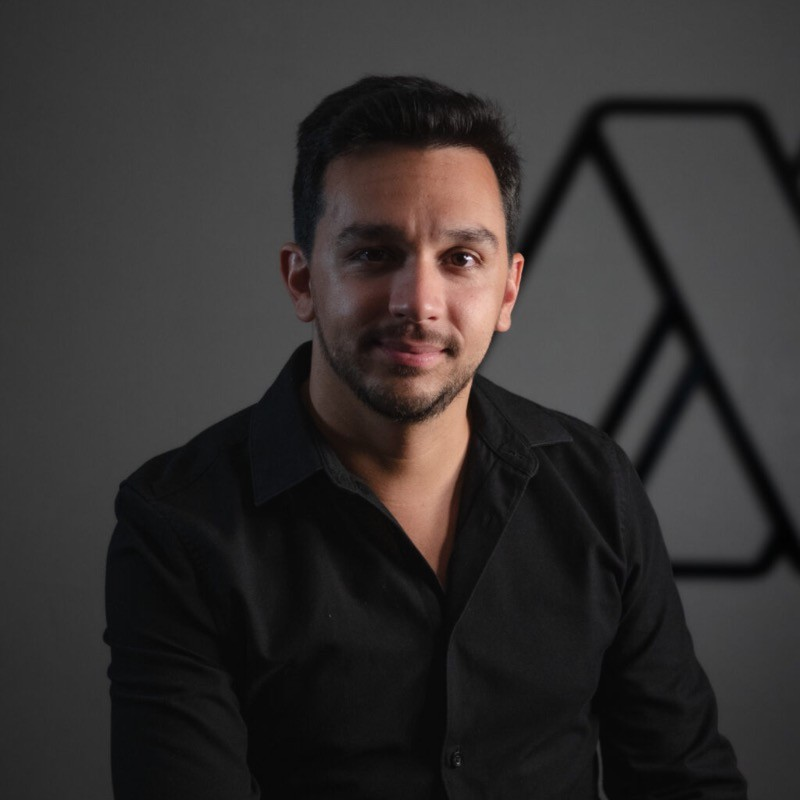
\includegraphics[width=1in,height=1.25in,clip,keepaspectratio]{bios/romano.jpeg}}]{Pedro S. Romano}
received the M.Sc. degree in telecommunications and computer engineering from Iscte -- Instituto
Universit\'ario de Lisboa, Lisbon, Portugal, where he is currently pursuing the Ph.D. degree. He has 11
years of experience in teaching and in mobile and web development. He is currently a University Teacher at
Iscte -- Instituto Universit\'ario de Lisboa, and an Executive Partner at AppX. His research focuses on
machine learning and artificial intelligence, on which he has published peer-reviewed machine-learning
studies; his interests also include mobile networks and software engineering.
\end{IEEEbiography}

\begin{IEEEbiography}[{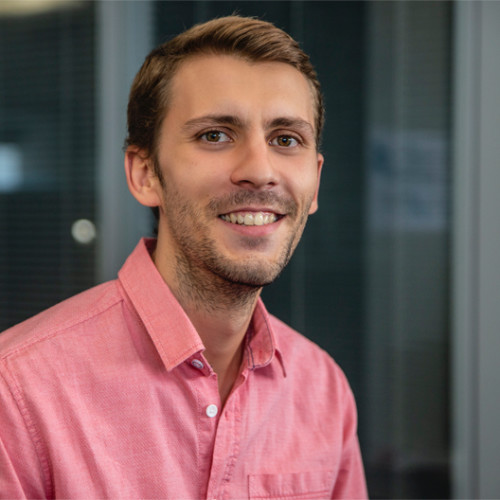
\includegraphics[width=1in,height=1.25in,clip,keepaspectratio]{bios/fernandes.jpeg}}]{Daniel F. S. Fernandes}
received the B.S. and M.S. degrees in telecommunications and computer engineering and the Ph.D. degree in
information science and technology from Iscte -- Instituto Universit\'ario de Lisboa, in 2012, 2017, and
2021, respectively. He is an Assistant Professor at Iscte -- Instituto Universit\'ario de Lisboa, and a
Researcher at Instituto de Telecomunica\c{c}\~oes, in the areas of computer science and
telecommunications. He has 11 scientific publications as an author in journals or international
conferences and 14 scientific publications as a co-author.
\end{IEEEbiography}

\begin{IEEEbiography}[{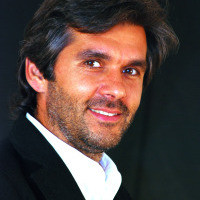
\includegraphics[width=1in,height=1.25in,clip,keepaspectratio]{bios/sebastiao.jpeg}}]{Pedro J. A. Sebasti\~ao}
(Member, IEEE) received the Ph.D. degree in electrical and computer engineering from Instituto Superior
T\'ecnico, Lisbon, Portugal. He is a Full Professor at Iscte -- Instituto Universit\'ario de Lisboa, where
he coordinates the curricular units of Technology-Based Project (Innovation and Entrepreneurship) and
Telecommunication Project (Telecommunication Engineering). He is the President of AUDAX-ISCTE, the
Innovation and Entrepreneurship Center, and has been responsible for several national and international
technological innovation projects involving knowledge and technology transfer. He has supervised or
co-supervised several M.Sc. and Ph.D. theses. He is the author or co-author of more than two hundred
scientific articles and of several e-books and handbooks on innovation and entrepreneurship in emergent
technologies. He has served as an expert and evaluator of more than one hundred national and international
research and development projects (defense and civil), and has received several scientific, engineering,
and teaching awards. He has supported technology-transfer projects leading to the creation of start-ups and
spin-offs, accompanying investment, pilots, and sales, has worked in the national defense industry, and was
responsible for communication technology systems in the Nokia Siemens business area. His research
interests include the monitoring, control, and communications of drones and unmanned vehicles,
telecommunication planning tools, stochastic-process modeling, efficient simulations, and efficient
communication systems.
\end{IEEEbiography}

\EOD

\end{document}
